\documentclass[10pt,a4paper]{article}
\usepackage{../sty/dm-editorial}
\usepackage{fontspec}
\usepackage{multicol}
% 문항 전사용 보조 매크로(dm-editorial 매크로를 덮어쓰지 않는다)
\newcommand{\pt}[1]{\mathrm{#1}}
\newcommand{\seg}[1]{\overline{\mathrm{#1}}}
\newcommand{\arc}[1]{\overset{\frown}{\mathrm{#1}}}
\newcommand{\vecAB}[1]{\overrightarrow{\mathrm{#1}}}
% 조건 상자. 본문에서는 수식을 안 끊지만(\binoppenalty) 이 상자는 폭이 고정이라 긴 식이 테두리 밖으로 삐져나간다
% (검수 지적 쎈B 대수 126-41·126-43·21-17 — 「(2n-1)·1」 끝이 상자 밖에 찍힌다). 상자 안에서만 연산자·관계 뒤 줄바꿈을 허용한다.
% 들어가는 식은 그대로 한 줄로 두고, 넘칠 때만 TeX 가 끊는다(원문도 그 자리에서 두 줄로 간다).
\newcommand{\exprbox}[1]{\par\smallskip\noindent\begin{center}\fbox{\begin{minipage}{0.96\linewidth}\centering\binoppenalty=700 \relpenalty=500 \vspace{1.5mm}#1\vspace{1.5mm}\end{minipage}}\end{center}}
% 여집합 · 「보기」 상자(ㄱ·ㄴ·ㄷ 참거짓 문항 — 줄바꿈은 \\)
\newcommand{\comp}[1]{{#1}^{\mathrm{c}}}
% 별도 줄 수식(원문의 가운데 줄): 좁은 낱장 폭보다 넓으면 폭에 맞게 줄인다(전사본의 \centerline 을 build 가 이것으로 바꾼다).
\newcommand{\dispeq}[1]{\centerline{\resizebox{\ifdim\width>\linewidth\linewidth\else\width\fi}{!}{#1}}}
% 보기 상자도 같다. ㄱ·ㄴ·ㄷ 줄은 \\ 로 나누므로 \parskip 이 먹지 않아, 분수가 든 줄이 다음 줄과 맞닿는다
% (검수 지적 쎈B 대수 62-08·78-40·79-46 · 미적분1 11-24·27-46). 줄 겹침 여유를 본문보다 넉넉히 주고, 긴 줄은 상자 안에서 끊는다.
\newcommand{\bogi}[1]{\par\smallskip\noindent\begin{center}\fbox{\begin{minipage}{0.96\linewidth}\binoppenalty=700 \relpenalty=500 \lineskiplimit=3pt \lineskip=4pt \vspace{1mm}{\small\bfseries 보기}\par\smallskip\setlength{\parskip}{0.6mm}#1\vspace{1mm}\end{minipage}}\end{center}}
\newcommand{\blank}[1][1.5em]{\raisebox{-0.15ex}{\framebox[#1]{\rule{0pt}{1.4ex}}}}
\newcommand{\dmhint}[1]{\par\smallskip\begin{tcolorbox}[enhanced,colback=dm-navylight!60,colframe=dm-navy!40,boxrule=0.3pt,sharp corners,left=3mm,right=3mm,top=2mm,bottom=2mm,boxsep=0mm]\small\setlength{\parskip}{1mm}#1\end{tcolorbox}}
% 구역 제목·공통 지시문은 뒤에 문항 한 개는 붙을 자리가 있어야 찍는다(쪽 끝 고아 방지).
\newcommand{\dmsection}[1]{\par\needspace{10\baselineskip}\vspace{3mm}\noindent{\color{dm-navy}\hrule height 0.6pt}\vspace{1.2mm}\noindent{\dmheadingfont\bfseries\fontsize{11}{13}\selectfont\color{dm-navy}#1}\par\vspace{4mm}}
% 지시문 뒤 4mm: 다음 문항의 출처 배지가 5mm 위로 올라오므로 긴 지시문 줄과 겹치지 않게 한다.
\newcommand{\dmpassage}[1]{\par\needspace{8\baselineskip}\medskip\noindent{\dmheadingfont\bfseries\color{dm-navy}#1}\par\vspace{4mm}}
% 줄바꿈 규약(프로토타입 mathbook-problems.sty · style.sty 와 같음): 수식 안에서는 줄을 바꾸지 않고, 「(단, …)」·「x축」은 한 덩어리.
\binoppenalty=10000 \relpenalty=10000
% 수식 안 글루는 늘이지 않는다. 낱장 폭(110mm)에서 긴 수식이 한 덩어리로 묶이면 남은 늘임이 \medmuskip·\thickmuskip 으로
% 들어가 「y  =  2x^2  -  3x」 처럼 연산자 둘레가 벌어진다(검수 지적 쎈B 공통수학1 95-42·95-44·130-35·136-67·26-68 등).
% 늘임은 낱말 사이로만 보낸다.
\thinmuskip=3mu \medmuskip=4mu \thickmuskip=5mu
\newlength{\dmfigw}
% 수식을 안 끊는 대신, 긴 수식 앞에서 줄을 바꾸면 앞 줄이 많이 비는 경우(RPM 중3-1 1022 지시문·0979)에 overfull 로 잘리지 않도록
% 비상 늘임 폭을 준다 — tolerance 안에서 조판되는 문단에는 영향이 없다.
\emergencystretch=2em
% 한글 음절 사이 늘임을 끈다. 좁은 낱장 폭(110mm)에 끊을 수 없는 긴 수식이 들어가면 kotex 가 남은 늘임을 음절 사이로
% 보내 「함 수 … 에 대 하 여」처럼 낱말이 무너진다(검수 지적 쎈B 미적분1 8-06·10-20·40-56·55-68 · 대수 51-36·54-64·90-11 등).
% 늘임은 낱말 사이로만 가게 하고, 그래도 모자라 줄이 넘치는 자리는 위 \emergencystretch 가 받는다.
% xetexko 는 음절마다 줄바꿈 자리를 두고 그 glue 에 plus.08em 을 주는데(xetexko.sty \XeKo@stretchshrink),
% 한 줄에 음절이 20개면 1.6em 까지 벌어진다. 늘임만 0 으로 두고 줄임(minus.04em)은 남겨 과밀 줄은 여전히 붙일 수 있게 한다.
\xetexkostretchshrink{plus0em minus.04em}
% 본문 속 \dfrac 처럼 키 큰 수식이 든 줄은 기본 \lineskip(1pt)으로는 위아래 줄과 맞닿는다
% (검수 지적 쎈B 미적분1 76-11·77-14·79-26·55-70·41-64 · 대수 62-08·36-34 등 — 분모가 아랫줄 글자 위에 올라탄다).
% 줄 사이가 2pt 보다 좁아지는 자리에서만 3pt 를 확보한다. 보통 줄은 \baselineskip 그대로라 쪽 배치가 바뀌지 않는다.
\lineskiplimit=2pt \lineskip=3pt
\newcommand{\nob}[1]{\mbox{#1}}
% 「(단, …)」 은 한 덩어리가 원칙이지만 그림 옆 좁은 폭(0.58)에서 긴 조건이 그림 뒤로 넘어가 잘리므로(RPM 공통수학2 0151),
% 「(단,」 만 첫 낱말에 붙이고 안쪽 낱말 사이에서는 줄을 바꿀 수 있게 둔다(수식 안은 여전히 안 끊긴다).
\newcommand{\cond}[1]{\mbox{(단,}\nobreakspace#1)}
% 본문 끝의 「(단, …)」(build 가 \cond 를 \dmcondfill{조건}{배점 상자} 로 바꾼 것): 같은 줄에 들어가면 그 줄 오른쪽 끝, 안 들어가면 다음 줄 오른쪽 끝에 두고
% 앞 줄은 fill 로 채워 어간이 벌어지지 않게 한다(TeXbook 의 증명 끝 기호 배치 · 검수 지적 개념원리 미적분Ⅱ 185-e19·106-e1 ⑴). 조건이 줄 폭(-2em)보다 넓으면
% (그림 옆 0.58 폭의 긴 조건) 예전처럼 「(단,」 만 앞 낱말에 붙이고 안쪽에서 줄을 바꾼다.
\newlength{\dmcondw}
\newcommand{\dmcondfill}[2]{%
  \settowidth{\dmcondw}{\mbox{(단,~#1)#2}}%
  \ifdim\dmcondw<\dimexpr\linewidth-2em\relax
    \unskip\nobreak\hfill\penalty0\hskip1.5em\hbox{}\nobreak\hfill\mbox{(단,~#1)#2}%
  \else
    \cond{#1}#2%
  \fi}
% 짧은 5지선다 한 줄 배치(원본이 보기 5개를 한 줄에 둔 것 · 검수 지적). \dmchoicesi 는 한 줄 5칸(칸 사이 fill · choices_layout "i" 강제).
% \dmchoicesauto{지주}{①}…{⑤} 는 build 가 시각 길이로 고른 후보를 TeX 이 실제 폭으로 재서, 칸 사이 최소 1.5em 으로 낱장 본문 폭(110mm 낱장 여백 6mm·번호 9mm
% 를 뺀 89mm · 현재 줄 폭이 더 좁으면 그 폭) 안에 들어가면 한 줄, 아니면 choices32(3+2 · 분수 지주 포함)로 되돌린다. 번호 기호는 sty 환경과 같은 \small.
\newlength{\dmchoicesw}\newlength{\dmchoiceslim}
\newcommand{\dmchoicesi}[5]{\par\medskip\noindent\mbox{\small ①\ #1}\hfill\mbox{\small ②\ #2}\hfill\mbox{\small ③\ #3}\hfill\mbox{\small ④\ #4}\hfill\mbox{\small ⑤\ #5}\par\medskip}
\newcommand{\dmchoicesauto}[6]{%
  \settowidth{\dmchoicesw}{\mbox{\small ①\ #2}\hskip1.5em\mbox{\small ②\ #3}\hskip1.5em\mbox{\small ③\ #4}\hskip1.5em\mbox{\small ④\ #5}\hskip1.5em\mbox{\small ⑤\ #6}}%
  \setlength{\dmchoiceslim}{\linewidth}\ifdim\dmchoiceslim>89mm \setlength{\dmchoiceslim}{89mm}\fi
  \ifdim\dmchoicesw<\dmchoiceslim \dmchoicesi{#2}{#3}{#4}{#5}{#6}\else\begin{choices32}{#1#2}{#1#3}{#1#4}{#1#5}{#1#6}\end{choices32}\fi}
\raggedbottom

\begin{document}
\renewcommand{\dmchapunit}{01 지수}
\dmchapter{01}{지수}
\setcounter{dmproblemcount}{0}
\dmsection{개념 01 거듭제곱}
\dmpassage{다음 식을 간단히 하시오. \cond{$a\ne 0$, $b\ne 0$}}
\setcounter{dmproblemcount}{0}\dmpnum{8-01}{% id: 8-01
% book: 베이직쎈 대수 · 01 지수
% section: 개념 01 거듭제곱
% passage: 다음 식을 간단히 하시오. \cond{$a\ne 0$, $b\ne 0$}
% figure: none
% answer: 
% answer_source: 
% variant_level: 0 (원본 전사)
% 이 파일은 build.mjs 가 items.json 에서 만든다. 고칠 때는 items.json 을 고친다.
\smash{\raisebox{1.5mm}{\dmkichul{베이직쎈 대수 8쪽 01번}}}
$a^3\times a^2$
}\vspace{8mm}
\setcounter{dmproblemcount}{1}\dmpnum{8-02}{% id: 8-02
% book: 베이직쎈 대수 · 01 지수
% section: 개념 01 거듭제곱
% passage: 다음 식을 간단히 하시오. \cond{$a\ne 0$, $b\ne 0$}
% figure: none
% answer: 
% answer_source: 
% variant_level: 0 (원본 전사)
% 이 파일은 build.mjs 가 items.json 에서 만든다. 고칠 때는 items.json 을 고친다.
\smash{\raisebox{1.5mm}{\dmkichul{베이직쎈 대수 8쪽 02번}}}
$(a^5)^4$
}\vspace{8mm}
\setcounter{dmproblemcount}{2}\dmpnum{8-03}{% id: 8-03
% book: 베이직쎈 대수 · 01 지수
% section: 개념 01 거듭제곱
% passage: 다음 식을 간단히 하시오. \cond{$a\ne 0$, $b\ne 0$}
% figure: none
% answer: 
% answer_source: 
% variant_level: 0 (원본 전사)
% 이 파일은 build.mjs 가 items.json 에서 만든다. 고칠 때는 items.json 을 고친다.
\smash{\raisebox{1.5mm}{\dmkichul{베이직쎈 대수 8쪽 03번}}}
$(ab)^3$
}\vspace{8mm}
\vspace{3mm}\setcounter{dmproblemcount}{3}\dmpnum{8-04}{% id: 8-04
% book: 베이직쎈 대수 · 01 지수
% section: 개념 01 거듭제곱
% passage: 다음 식을 간단히 하시오. \cond{$a\ne 0$, $b\ne 0$}
% figure: none
% answer: 
% answer_source: 
% variant_level: 0 (원본 전사)
% 이 파일은 build.mjs 가 items.json 에서 만든다. 고칠 때는 items.json 을 고친다.
\smash{\raisebox{4.5mm}{\dmkichul{베이직쎈 대수 8쪽 04번}}}
$\left(\dfrac{a}{b}\right)^{5}$
}\vspace{8mm}
\setcounter{dmproblemcount}{4}\dmpnum{8-05}{% id: 8-05
% book: 베이직쎈 대수 · 01 지수
% section: 개념 01 거듭제곱
% passage: 다음 식을 간단히 하시오. \cond{$a\ne 0$, $b\ne 0$}
% figure: none
% answer: 
% answer_source: 
% variant_level: 0 (원본 전사)
% 이 파일은 build.mjs 가 items.json 에서 만든다. 고칠 때는 items.json 을 고친다.
\smash{\raisebox{1.5mm}{\dmkichul{베이직쎈 대수 8쪽 05번}}}
$a^6\div a^3$
}\vspace{8mm}
\setcounter{dmproblemcount}{5}\dmpnum{8-06}{% id: 8-06
% book: 베이직쎈 대수 · 01 지수
% section: 개념 01 거듭제곱
% passage: 다음 식을 간단히 하시오. \cond{$a\ne 0$, $b\ne 0$}
% figure: none
% answer: 
% answer_source: 
% variant_level: 0 (원본 전사)
% 이 파일은 build.mjs 가 items.json 에서 만든다. 고칠 때는 items.json 을 고친다.
\smash{\raisebox{1.5mm}{\dmkichul{베이직쎈 대수 8쪽 06번}}}
$a^7\div a^7$
}\vspace{8mm}
\setcounter{dmproblemcount}{6}\dmpnum{8-07}{% id: 8-07
% book: 베이직쎈 대수 · 01 지수
% section: 개념 01 거듭제곱
% passage: 다음 식을 간단히 하시오. \cond{$a\ne 0$, $b\ne 0$}
% figure: none
% answer: 
% answer_source: 
% variant_level: 0 (원본 전사)
% 이 파일은 build.mjs 가 items.json 에서 만든다. 고칠 때는 items.json 을 고친다.
\smash{\raisebox{1.5mm}{\dmkichul{베이직쎈 대수 8쪽 07번}}}
$a^2\div a^8$
}\vspace{8mm}
\setcounter{dmproblemcount}{7}\dmpnum{8-08}{% id: 8-08
% book: 베이직쎈 대수 · 01 지수
% section: 개념 01 거듭제곱
% passage: 다음 식을 간단히 하시오. \cond{$a\ne 0$, $b\ne 0$}
% figure: none
% answer: 
% answer_source: 
% variant_level: 0 (원본 전사)
% 이 파일은 build.mjs 가 items.json 에서 만든다. 고칠 때는 items.json 을 고친다.
\smash{\raisebox{1.5mm}{\dmkichul{베이직쎈 대수 8쪽 08번}}}
$ab^5\times a^2b^4$
\dmhint{밑이 같은 것끼리 지수법칙을 적용해.}
}\vspace{8mm}
\setcounter{dmproblemcount}{8}\dmpnum{8-09}{% id: 8-09
% book: 베이직쎈 대수 · 01 지수
% section: 개념 01 거듭제곱
% passage: 다음 식을 간단히 하시오. \cond{$a\ne 0$, $b\ne 0$}
% figure: none
% answer: 
% answer_source: 
% variant_level: 0 (원본 전사)
% 이 파일은 build.mjs 가 items.json 에서 만든다. 고칠 때는 items.json 을 고친다.
\smash{\raisebox{1.5mm}{\dmkichul{베이직쎈 대수 8쪽 09번}}}
$a^4\times a^3b\times b^5$
}\vspace{8mm}
\setcounter{dmproblemcount}{9}\dmpnum{8-10}{% id: 8-10
% book: 베이직쎈 대수 · 01 지수
% section: 개념 01 거듭제곱
% passage: 다음 식을 간단히 하시오. \cond{$a\ne 0$, $b\ne 0$}
% figure: none
% answer: 
% answer_source: 
% variant_level: 0 (원본 전사)
% 이 파일은 build.mjs 가 items.json 에서 만든다. 고칠 때는 items.json 을 고친다.
\smash{\raisebox{1.5mm}{\dmkichul{베이직쎈 대수 8쪽 10번}}}
$(ab)^4\times(a^2b)^3$
}\vspace{8mm}
\vspace{3mm}\setcounter{dmproblemcount}{10}\dmpnum{8-11}{% id: 8-11
% book: 베이직쎈 대수 · 01 지수
% section: 개념 01 거듭제곱
% passage: 다음 식을 간단히 하시오. \cond{$a\ne 0$, $b\ne 0$}
% figure: none
% answer: 
% answer_source: 
% variant_level: 0 (원본 전사)
% 이 파일은 build.mjs 가 items.json 에서 만든다. 고칠 때는 items.json 을 고친다.
\smash{\raisebox{4.5mm}{\dmkichul{베이직쎈 대수 8쪽 11번}}}
$\left(\dfrac{a}{b^2}\right)^{2}\times\left(\dfrac{b}{a}\right)^{6}$
}\vspace{8mm}
\setcounter{dmproblemcount}{11}\dmpnum{8-12}{% id: 8-12
% book: 베이직쎈 대수 · 01 지수
% section: 개념 01 거듭제곱
% passage: 다음 식을 간단히 하시오. \cond{$a\ne 0$, $b\ne 0$}
% figure: none
% answer: 
% answer_source: 
% variant_level: 0 (원본 전사)
% 이 파일은 build.mjs 가 items.json 에서 만든다. 고칠 때는 items.json 을 고친다.
\smash{\raisebox{1.5mm}{\dmkichul{베이직쎈 대수 8쪽 12번}}}
$(-2a^3b^2)^4\div(2ab)^3$
}\vspace{8mm}
\vspace{3mm}\setcounter{dmproblemcount}{12}\dmpnum{8-13}{% id: 8-13
% book: 베이직쎈 대수 · 01 지수
% section: 개념 01 거듭제곱
% passage: 다음 식을 간단히 하시오. \cond{$a\ne 0$, $b\ne 0$}
% figure: none
% answer: 
% answer_source: 
% variant_level: 0 (원본 전사)
% 이 파일은 build.mjs 가 items.json 에서 만든다. 고칠 때는 items.json 을 고친다.
\smash{\raisebox{4.5mm}{\dmkichul{베이직쎈 대수 8쪽 13번}}}
$5a^3b^5\div\left(\dfrac{3a}{b^2}\right)^{2}$
}\vspace{8mm}
\vspace{3mm}\setcounter{dmproblemcount}{13}\dmpnum{8-14}{% id: 8-14
% book: 베이직쎈 대수 · 01 지수
% section: 개념 01 거듭제곱
% passage: 다음 식을 간단히 하시오. \cond{$a\ne 0$, $b\ne 0$}
% figure: none
% answer: 
% answer_source: 
% variant_level: 0 (원본 전사)
% 이 파일은 build.mjs 가 items.json 에서 만든다. 고칠 때는 items.json 을 고친다.
\smash{\raisebox{4.5mm}{\dmkichul{베이직쎈 대수 8쪽 14번}}}
$6a^7b^2\times 5ab^2\div\left(\dfrac{a^2}{b}\right)^{3}$
}\vspace{8mm}
\dmsection{개념 02 거듭제곱근}
\dmpassage{다음 거듭제곱근을 구하시오.}
\setcounter{dmproblemcount}{14}\dmpnum{9-15}{% id: 9-15
% book: 베이직쎈 대수 · 01 지수
% section: 개념 02 거듭제곱근
% passage: 다음 거듭제곱근을 구하시오.
% figure: none
% answer: 
% answer_source: 
% variant_level: 0 (원본 전사)
% 이 파일은 build.mjs 가 items.json 에서 만든다. 고칠 때는 items.json 을 고친다.
\smash{\raisebox{1.5mm}{\dmkichul{베이직쎈 대수 9쪽 15번}}}
$9$의 제곱근
}\vspace{8mm}
\setcounter{dmproblemcount}{15}\dmpnum{9-16}{% id: 9-16
% book: 베이직쎈 대수 · 01 지수
% section: 개념 02 거듭제곱근
% passage: 다음 거듭제곱근을 구하시오.
% figure: none
% answer: 
% answer_source: 
% variant_level: 0 (원본 전사)
% 이 파일은 build.mjs 가 items.json 에서 만든다. 고칠 때는 items.json 을 고친다.
\smash{\raisebox{1.5mm}{\dmkichul{베이직쎈 대수 9쪽 16번}}}
$1$의 세제곱근
\dmhint{$1$의 세제곱근을 $x$라 하면 $x^3=1$이므로\\ $x^3-1=0$, \quad $(x-1)(\blank[2.4em])=0$\\ $\therefore\ x=1$ 또는 $x=\blank[2.4em]$\\ 따라서 $1$의 세제곱근은 $1$, $\blank[2.4em]$, $\blank[2.4em]$이다.}
}\vspace{8mm}
\setcounter{dmproblemcount}{16}\dmpnum{9-17}{% id: 9-17
% book: 베이직쎈 대수 · 01 지수
% section: 개념 02 거듭제곱근
% passage: 다음 거듭제곱근을 구하시오.
% figure: none
% answer: 
% answer_source: 
% variant_level: 0 (원본 전사)
% 이 파일은 build.mjs 가 items.json 에서 만든다. 고칠 때는 items.json 을 고친다.
\smash{\raisebox{1.5mm}{\dmkichul{베이직쎈 대수 9쪽 17번}}}
$-8$의 세제곱근
}\vspace{8mm}
\setcounter{dmproblemcount}{17}\dmpnum{9-18}{% id: 9-18
% book: 베이직쎈 대수 · 01 지수
% section: 개념 02 거듭제곱근
% passage: 다음 거듭제곱근을 구하시오.
% figure: none
% answer: 
% answer_source: 
% variant_level: 0 (원본 전사)
% 이 파일은 build.mjs 가 items.json 에서 만든다. 고칠 때는 items.json 을 고친다.
\smash{\raisebox{1.5mm}{\dmkichul{베이직쎈 대수 9쪽 18번}}}
$16$의 네제곱근
}\vspace{8mm}
\setcounter{dmproblemcount}{18}\dmpnum{9-19}{% id: 9-19
% book: 베이직쎈 대수 · 01 지수
% section: 개념 02 거듭제곱근
% passage: 다음 거듭제곱근을 구하시오.
% figure: none
% answer: 
% answer_source: 
% variant_level: 0 (원본 전사)
% 이 파일은 build.mjs 가 items.json 에서 만든다. 고칠 때는 items.json 을 고친다.
\smash{\raisebox{1.5mm}{\dmkichul{베이직쎈 대수 9쪽 19번}}}
$256$의 네제곱근
}\vspace{8mm}
\dmpassage{다음 거듭제곱근 중 실수인 것을 구하시오.}
\setcounter{dmproblemcount}{19}\dmpnum{9-20}{% id: 9-20
% book: 베이직쎈 대수 · 01 지수
% section: 개념 02 거듭제곱근
% passage: 다음 거듭제곱근 중 실수인 것을 구하시오.
% figure: none
% answer: 
% answer_source: 
% variant_level: 0 (원본 전사)
% 이 파일은 build.mjs 가 items.json 에서 만든다. 고칠 때는 items.json 을 고친다.
\smash{\raisebox{1.5mm}{\dmkichul{베이직쎈 대수 9쪽 20번}}}
$49$의 제곱근
}\vspace{8mm}
\setcounter{dmproblemcount}{20}\dmpnum{9-21}{% id: 9-21
% book: 베이직쎈 대수 · 01 지수
% section: 개념 02 거듭제곱근
% passage: 다음 거듭제곱근 중 실수인 것을 구하시오.
% figure: none
% answer: 
% answer_source: 
% variant_level: 0 (원본 전사)
% 이 파일은 build.mjs 가 items.json 에서 만든다. 고칠 때는 items.json 을 고친다.
\smash{\raisebox{1.5mm}{\dmkichul{베이직쎈 대수 9쪽 21번}}}
$-1$의 세제곱근
}\vspace{8mm}
\setcounter{dmproblemcount}{21}\dmpnum{10-22}{% id: 10-22
% book: 베이직쎈 대수 · 01 지수
% section: 개념 02 거듭제곱근
% figure: none
% answer: 
% answer_source: 
% variant_level: 0 (원본 전사)
% 이 파일은 build.mjs 가 items.json 에서 만든다. 고칠 때는 items.json 을 고친다.
\smash{\raisebox{1.5mm}{\dmkichul{베이직쎈 대수 10쪽 22번}}}
27의 세제곱근
}\vspace{8mm}
\setcounter{dmproblemcount}{22}\dmpnum{10-23}{% id: 10-23
% book: 베이직쎈 대수 · 01 지수
% section: 개념 02 거듭제곱근
% figure: none
% answer: 
% answer_source: 
% variant_level: 0 (원본 전사)
% 이 파일은 build.mjs 가 items.json 에서 만든다. 고칠 때는 items.json 을 고친다.
\smash{\raisebox{1.5mm}{\dmkichul{베이직쎈 대수 10쪽 23번}}}
81의 네제곱근
}\vspace{8mm}
\setcounter{dmproblemcount}{23}\dmpnum{10-24}{% id: 10-24
% book: 베이직쎈 대수 · 01 지수
% section: 개념 02 거듭제곱근
% figure: none
% answer: 
% answer_source: 
% variant_level: 0 (원본 전사)
% 이 파일은 build.mjs 가 items.json 에서 만든다. 고칠 때는 items.json 을 고친다.
\smash{\raisebox{1.5mm}{\dmkichul{베이직쎈 대수 10쪽 24번}}}
$-16$의 네제곱근
}\vspace{8mm}
\dmpassage{다음을 간단히 하시오.}
\vspace{3mm}\setcounter{dmproblemcount}{24}\dmpnum{10-25}{% id: 10-25
% book: 베이직쎈 대수 · 01 지수
% section: 개념 02 거듭제곱근
% passage: 다음을 간단히 하시오.
% figure: none
% answer: 
% answer_source: 
% variant_level: 0 (원본 전사)
% 이 파일은 build.mjs 가 items.json 에서 만든다. 고칠 때는 items.json 을 고친다.
\smash{\raisebox{4.5mm}{\dmkichul{베이직쎈 대수 10쪽 25번}}}
$\sqrt[3]{125}$
}\vspace{8mm}
\vspace{3mm}\setcounter{dmproblemcount}{25}\dmpnum{10-26}{% id: 10-26
% book: 베이직쎈 대수 · 01 지수
% section: 개념 02 거듭제곱근
% passage: 다음을 간단히 하시오.
% figure: none
% answer: 
% answer_source: 
% variant_level: 0 (원본 전사)
% 이 파일은 build.mjs 가 items.json 에서 만든다. 고칠 때는 items.json 을 고친다.
\smash{\raisebox{4.5mm}{\dmkichul{베이직쎈 대수 10쪽 26번}}}
$-\sqrt[4]{256}$
}\vspace{8mm}
\vspace{3mm}\setcounter{dmproblemcount}{26}\dmpnum{10-27}{% id: 10-27
% book: 베이직쎈 대수 · 01 지수
% section: 개념 02 거듭제곱근
% passage: 다음을 간단히 하시오.
% figure: none
% answer: 
% answer_source: 
% variant_level: 0 (원본 전사)
% 이 파일은 build.mjs 가 items.json 에서 만든다. 고칠 때는 items.json 을 고친다.
\smash{\raisebox{4.5mm}{\dmkichul{베이직쎈 대수 10쪽 27번}}}
$\sqrt[5]{-32}$
}\vspace{8mm}
\vspace{3mm}\setcounter{dmproblemcount}{27}\dmpnum{10-28}{% id: 10-28
% book: 베이직쎈 대수 · 01 지수
% section: 개념 02 거듭제곱근
% passage: 다음을 간단히 하시오.
% figure: none
% answer: 
% answer_source: 
% variant_level: 0 (원본 전사)
% 이 파일은 build.mjs 가 items.json 에서 만든다. 고칠 때는 items.json 을 고친다.
\smash{\raisebox{4.5mm}{\dmkichul{베이직쎈 대수 10쪽 28번}}}
$\sqrt[4]{0.0001}$
}\vspace{8mm}
\vspace{3mm}\setcounter{dmproblemcount}{28}\dmpnum{10-29}{% id: 10-29
% book: 베이직쎈 대수 · 01 지수
% section: 개념 02 거듭제곱근
% passage: 다음을 간단히 하시오.
% figure: none
% answer: 
% answer_source: 
% variant_level: 0 (원본 전사)
% 이 파일은 build.mjs 가 items.json 에서 만든다. 고칠 때는 items.json 을 고친다.
\smash{\raisebox{4.5mm}{\dmkichul{베이직쎈 대수 10쪽 29번}}}
$\sqrt[3]{0.216}$
}\vspace{8mm}
\vspace{3mm}\setcounter{dmproblemcount}{29}\dmpnum{10-30}{% id: 10-30
% book: 베이직쎈 대수 · 01 지수
% section: 개념 02 거듭제곱근
% passage: 다음을 간단히 하시오.
% figure: none
% answer: 
% answer_source: 
% variant_level: 0 (원본 전사)
% 이 파일은 build.mjs 가 items.json 에서 만든다. 고칠 때는 items.json 을 고친다.
\smash{\raisebox{4.5mm}{\dmkichul{베이직쎈 대수 10쪽 30번}}}
$\sqrt[3]{-\dfrac{8}{27}}$
}\vspace{8mm}
\dmpassage{다음 중 옳은 것은 ‘$\bigcirc$’를, 옳지 않은 것은 ‘$\times$’를 (\hspace*{1.2em}) 안에 써넣으시오.}
\setcounter{dmproblemcount}{30}\dmpnum{10-31}{% id: 10-31
% book: 베이직쎈 대수 · 01 지수
% section: 개념 02 거듭제곱근
% passage: 다음 중 옳은 것은 ‘$\bigcirc$’를, 옳지 않은 것은 ‘$\times$’를 (\hspace*{1.2em}) 안에 써넣으시오.
% figure: none
% answer: 
% answer_source: 
% variant_level: 0 (원본 전사)
% 이 파일은 build.mjs 가 items.json 에서 만든다. 고칠 때는 items.json 을 고친다.
\smash{\raisebox{1.5mm}{\dmkichul{베이직쎈 대수 10쪽 31번}}}
625의 네제곱근은 $\pm5i$, $\pm5$이다. \hfill (\hspace*{2.4em})
}\vspace{8mm}
\setcounter{dmproblemcount}{31}\dmpnum{10-32}{% id: 10-32
% book: 베이직쎈 대수 · 01 지수
% section: 개념 02 거듭제곱근
% passage: 다음 중 옳은 것은 ‘$\bigcirc$’를, 옳지 않은 것은 ‘$\times$’를 (\hspace*{1.2em}) 안에 써넣으시오.
% figure: none
% answer: 
% answer_source: 
% variant_level: 0 (원본 전사)
% 이 파일은 build.mjs 가 items.json 에서 만든다. 고칠 때는 items.json 을 고친다.
\smash{\raisebox{1.5mm}{\dmkichul{베이직쎈 대수 10쪽 32번}}}
0의 네제곱근 중 실수인 것은 없다. \hfill (\hspace*{2.4em})
}\vspace{8mm}
\setcounter{dmproblemcount}{32}\dmpnum{10-33}{% id: 10-33
% book: 베이직쎈 대수 · 01 지수
% section: 개념 02 거듭제곱근
% passage: 다음 중 옳은 것은 ‘$\bigcirc$’를, 옳지 않은 것은 ‘$\times$’를 (\hspace*{1.2em}) 안에 써넣으시오.
% figure: none
% answer: 
% answer_source: 
% variant_level: 0 (원본 전사)
% 이 파일은 build.mjs 가 items.json 에서 만든다. 고칠 때는 items.json 을 고친다.
\smash{\raisebox{1.5mm}{\dmkichul{베이직쎈 대수 10쪽 33번}}}
$-5$의 세제곱근 중 실수인 것은 1개이다. \hfill (\hspace*{2.4em})
}\vspace{8mm}
\vspace{3mm}\setcounter{dmproblemcount}{33}\dmpnum{10-34}{% id: 10-34
% book: 베이직쎈 대수 · 01 지수
% section: 개념 02 거듭제곱근
% passage: 다음 중 옳은 것은 ‘$\bigcirc$’를, 옳지 않은 것은 ‘$\times$’를 (\hspace*{1.2em}) 안에 써넣으시오.
% figure: none
% answer: 
% answer_source: 
% variant_level: 0 (원본 전사)
% 이 파일은 build.mjs 가 items.json 에서 만든다. 고칠 때는 items.json 을 고친다.
\smash{\raisebox{4.5mm}{\dmkichul{베이직쎈 대수 10쪽 34번}}}
$-49$의 네제곱근 중 실수인 것은 $-\sqrt{7}$, $\sqrt{7}$이다. \hfill (\hspace*{2.4em})
}\vspace{8mm}
\setcounter{dmproblemcount}{34}\dmpnum{10-35}{% id: 10-35
% book: 베이직쎈 대수 · 01 지수
% section: 개념 02 거듭제곱근
% passage: 다음 중 옳은 것은 ‘$\bigcirc$’를, 옳지 않은 것은 ‘$\times$’를 (\hspace*{1.2em}) 안에 써넣으시오.
% figure: none
% answer: 
% answer_source: 
% variant_level: 0 (원본 전사)
% 이 파일은 build.mjs 가 items.json 에서 만든다. 고칠 때는 items.json 을 고친다.
\smash{\raisebox{1.5mm}{\dmkichul{베이직쎈 대수 10쪽 35번}}}
$-8$의 네제곱근은 4개이다. \hfill (\hspace*{2.4em})
}\vspace{8mm}
\dmsection{개념 03 거듭제곱근의 성질}
\dmpassage{다음 식을 간단히 하시오.}
\vspace{3mm}\setcounter{dmproblemcount}{35}\dmpnum{11-36}{% id: 11-36
% book: 베이직쎈 대수 · 01 지수
% section: 개념 03 거듭제곱근의 성질
% passage: 다음 식을 간단히 하시오.
% figure: none
% answer: 
% answer_source: 
% variant_level: 0 (원본 전사)
% 이 파일은 build.mjs 가 items.json 에서 만든다. 고칠 때는 items.json 을 고친다.
\smash{\raisebox{4.5mm}{\dmkichul{베이직쎈 대수 11쪽 36번}}}
$\sqrt[3]{4}\mkern3mu \sqrt[3]{16}$
}\vspace{8mm}
\vspace{3mm}\setcounter{dmproblemcount}{36}\dmpnum{11-37}{% id: 11-37
% book: 베이직쎈 대수 · 01 지수
% section: 개념 03 거듭제곱근의 성질
% passage: 다음 식을 간단히 하시오.
% figure: none
% answer: 
% answer_source: 
% variant_level: 0 (원본 전사)
% 이 파일은 build.mjs 가 items.json 에서 만든다. 고칠 때는 items.json 을 고친다.
\smash{\raisebox{4.5mm}{\dmkichul{베이직쎈 대수 11쪽 37번}}}
$\sqrt[5]{27}\mkern3mu \sqrt[5]{9}$
}\vspace{8mm}
\vspace{3mm}\setcounter{dmproblemcount}{37}\dmpnum{11-38}{% id: 11-38
% book: 베이직쎈 대수 · 01 지수
% section: 개념 03 거듭제곱근의 성질
% passage: 다음 식을 간단히 하시오.
% figure: none
% answer: 
% answer_source: 
% variant_level: 0 (원본 전사)
% 이 파일은 build.mjs 가 items.json 에서 만든다. 고칠 때는 items.json 을 고친다.
\smash{\raisebox{4.5mm}{\dmkichul{베이직쎈 대수 11쪽 38번}}}
$\sqrt[4]{\dfrac{1}{4}}\mkern3mu \sqrt[4]{\dfrac{1}{64}}$
}\vspace{8mm}
\vspace{3mm}\setcounter{dmproblemcount}{38}\dmpnum{11-39}{% id: 11-39
% book: 베이직쎈 대수 · 01 지수
% section: 개념 03 거듭제곱근의 성질
% passage: 다음 식을 간단히 하시오.
% figure: none
% answer: 
% answer_source: 
% variant_level: 0 (원본 전사)
% 이 파일은 build.mjs 가 items.json 에서 만든다. 고칠 때는 items.json 을 고친다.
\smash{\raisebox{4.5mm}{\dmkichul{베이직쎈 대수 11쪽 39번}}}
$\dfrac{\sqrt[6]{128}}{\sqrt[6]{2}}$
}\vspace{8mm}
\vspace{3mm}\setcounter{dmproblemcount}{39}\dmpnum{11-40}{% id: 11-40
% book: 베이직쎈 대수 · 01 지수
% section: 개념 03 거듭제곱근의 성질
% passage: 다음 식을 간단히 하시오.
% figure: none
% answer: 
% answer_source: 
% variant_level: 0 (원본 전사)
% 이 파일은 build.mjs 가 items.json 에서 만든다. 고칠 때는 items.json 을 고친다.
\smash{\raisebox{4.5mm}{\dmkichul{베이직쎈 대수 11쪽 40번}}}
$\dfrac{\sqrt[4]{243}}{\sqrt[4]{3}}$
}\vspace{8mm}
\vspace{3mm}\setcounter{dmproblemcount}{40}\dmpnum{11-41}{% id: 11-41
% book: 베이직쎈 대수 · 01 지수
% section: 개념 03 거듭제곱근의 성질
% passage: 다음 식을 간단히 하시오.
% figure: none
% answer: 
% answer_source: 
% variant_level: 0 (원본 전사)
% 이 파일은 build.mjs 가 items.json 에서 만든다. 고칠 때는 items.json 을 고친다.
\smash{\raisebox{4.5mm}{\dmkichul{베이직쎈 대수 11쪽 41번}}}
$\dfrac{\sqrt[3]{5}}{\sqrt[3]{625}}$
}\vspace{8mm}
\vspace{3mm}\setcounter{dmproblemcount}{41}\dmpnum{11-42}{% id: 11-42
% book: 베이직쎈 대수 · 01 지수
% section: 개념 03 거듭제곱근의 성질
% passage: 다음 식을 간단히 하시오.
% figure: none
% answer: 
% answer_source: 
% variant_level: 0 (원본 전사)
% 이 파일은 build.mjs 가 items.json 에서 만든다. 고칠 때는 items.json 을 고친다.
\smash{\raisebox{4.5mm}{\dmkichul{베이직쎈 대수 11쪽 42번}}}
$\dfrac{\sqrt[5]{0.0001}}{\sqrt[5]{10}}$
}\vspace{8mm}
\vspace{3mm}\setcounter{dmproblemcount}{42}\dmpnum{11-43}{% id: 11-43
% book: 베이직쎈 대수 · 01 지수
% section: 개념 03 거듭제곱근의 성질
% passage: 다음 식을 간단히 하시오.
% figure: none
% answer: 
% answer_source: 
% variant_level: 0 (원본 전사)
% 이 파일은 build.mjs 가 items.json 에서 만든다. 고칠 때는 items.json 을 고친다.
\smash{\raisebox{4.5mm}{\dmkichul{베이직쎈 대수 11쪽 43번}}}
$(\sqrt[7]{16}\mkern3mu )^{7}$
}\vspace{8mm}
\vspace{3mm}\setcounter{dmproblemcount}{43}\dmpnum{11-44}{% id: 11-44
% book: 베이직쎈 대수 · 01 지수
% section: 개념 03 거듭제곱근의 성질
% passage: 다음 식을 간단히 하시오.
% figure: none
% answer: 
% answer_source: 
% variant_level: 0 (원본 전사)
% 이 파일은 build.mjs 가 items.json 에서 만든다. 고칠 때는 items.json 을 고친다.
\smash{\raisebox{4.5mm}{\dmkichul{베이직쎈 대수 11쪽 44번}}}
$(\sqrt[6]{49}\mkern3mu )^{3}$
}\vspace{8mm}
\vspace{3mm}\setcounter{dmproblemcount}{44}\dmpnum{11-45}{% id: 11-45
% book: 베이직쎈 대수 · 01 지수
% section: 개념 03 거듭제곱근의 성질
% passage: 다음 식을 간단히 하시오.
% figure: none
% answer: 
% answer_source: 
% variant_level: 0 (원본 전사)
% 이 파일은 build.mjs 가 items.json 에서 만든다. 고칠 때는 items.json 을 고친다.
\smash{\raisebox{4.5mm}{\dmkichul{베이직쎈 대수 11쪽 45번}}}
$\left(\sqrt[8]{\dfrac{1}{9}}\mkern3mu \right)^{4}$
}\vspace{8mm}
\vspace{3mm}\setcounter{dmproblemcount}{45}\dmpnum{11-46}{% id: 11-46
% book: 베이직쎈 대수 · 01 지수
% section: 개념 03 거듭제곱근의 성질
% passage: 다음 식을 간단히 하시오.
% figure: none
% answer: 
% answer_source: 
% variant_level: 0 (원본 전사)
% 이 파일은 build.mjs 가 items.json 에서 만든다. 고칠 때는 items.json 을 고친다.
\smash{\raisebox{4.5mm}{\dmkichul{베이직쎈 대수 11쪽 46번}}}
$\sqrt[3]{\sqrt{64}}$
}\vspace{8mm}
\vspace{3mm}\setcounter{dmproblemcount}{46}\dmpnum{11-47}{% id: 11-47
% book: 베이직쎈 대수 · 01 지수
% section: 개념 03 거듭제곱근의 성질
% passage: 다음 식을 간단히 하시오.
% figure: none
% answer: 
% answer_source: 
% variant_level: 0 (원본 전사)
% 이 파일은 build.mjs 가 items.json 에서 만든다. 고칠 때는 items.json 을 고친다.
\smash{\raisebox{4.5mm}{\dmkichul{베이직쎈 대수 11쪽 47번}}}
$\sqrt{\sqrt{625}}$
}\vspace{8mm}
\vspace{3mm}\setcounter{dmproblemcount}{47}\dmpnum{12-48}{% id: 12-48
% book: 베이직쎈 대수 · 01 지수
% section: 개념 03 거듭제곱근의 성질
% passage: 다음 식을 간단히 하시오.
% figure: none
% answer: 
% answer_source: 
% variant_level: 0 (원본 전사)
% 이 파일은 build.mjs 가 items.json 에서 만든다. 고칠 때는 items.json 을 고친다.
\smash{\raisebox{4.5mm}{\dmkichul{베이직쎈 대수 12쪽 48번}}}
$\sqrt[3]{\sqrt[5]{8}}$
}\vspace{8mm}
\vspace{3mm}\setcounter{dmproblemcount}{48}\dmpnum{12-49}{% id: 12-49
% book: 베이직쎈 대수 · 01 지수
% section: 개념 03 거듭제곱근의 성질
% passage: 다음 식을 간단히 하시오.
% figure: none
% answer: 
% answer_source: 
% variant_level: 0 (원본 전사)
% 이 파일은 build.mjs 가 items.json 에서 만든다. 고칠 때는 items.json 을 고친다.
\smash{\raisebox{4.5mm}{\dmkichul{베이직쎈 대수 12쪽 49번}}}
$\sqrt[4]{25^2}$
}\vspace{8mm}
\vspace{3mm}\setcounter{dmproblemcount}{49}\dmpnum{12-50}{% id: 12-50
% book: 베이직쎈 대수 · 01 지수
% section: 개념 03 거듭제곱근의 성질
% passage: 다음 식을 간단히 하시오.
% figure: none
% answer: 
% answer_source: 
% variant_level: 0 (원본 전사)
% 이 파일은 build.mjs 가 items.json 에서 만든다. 고칠 때는 items.json 을 고친다.
\smash{\raisebox{4.5mm}{\dmkichul{베이직쎈 대수 12쪽 50번}}}
$\sqrt[4]{\left(\dfrac{1}{4}\right)^{6}}$
}\vspace{8mm}
\vspace{3mm}\setcounter{dmproblemcount}{50}\dmpnum{12-51}{% id: 12-51
% book: 베이직쎈 대수 · 01 지수
% section: 개념 03 거듭제곱근의 성질
% passage: 다음 식을 간단히 하시오.
% figure: none
% answer: 
% answer_source: 
% variant_level: 0 (원본 전사)
% 이 파일은 build.mjs 가 items.json 에서 만든다. 고칠 때는 items.json 을 고친다.
\smash{\raisebox{4.5mm}{\dmkichul{베이직쎈 대수 12쪽 51번}}}
$\left(\sqrt[10]{7}\right)^{5}$
}\vspace{8mm}
\dmpassage{$a>0$, $b>0$일 때, 다음 식을 간단히 하시오.}
\vspace{3mm}\setcounter{dmproblemcount}{51}\dmpnum{12-52}{% id: 12-52
% book: 베이직쎈 대수 · 01 지수
% section: 개념 03 거듭제곱근의 성질
% passage: $a>0$, $b>0$일 때, 다음 식을 간단히 하시오.
% figure: none
% answer: 
% answer_source: 
% variant_level: 0 (원본 전사)
% 이 파일은 build.mjs 가 items.json 에서 만든다. 고칠 때는 items.json 을 고친다.
\smash{\raisebox{4.5mm}{\dmkichul{베이직쎈 대수 12쪽 52번}}}
$\sqrt[8]{a^5}\times\sqrt[8]{a^3}$
}\vspace{8mm}
\vspace{3mm}\setcounter{dmproblemcount}{52}\dmpnum{12-53}{% id: 12-53
% book: 베이직쎈 대수 · 01 지수
% section: 개념 03 거듭제곱근의 성질
% passage: $a>0$, $b>0$일 때, 다음 식을 간단히 하시오.
% figure: none
% answer: 
% answer_source: 
% variant_level: 0 (원본 전사)
% 이 파일은 build.mjs 가 items.json 에서 만든다. 고칠 때는 items.json 을 고친다.
\smash{\raisebox{4.5mm}{\dmkichul{베이직쎈 대수 12쪽 53번}}}
$\dfrac{\sqrt{a^6}}{\sqrt{a^2}}$
}\vspace{8mm}
\vspace{3mm}\setcounter{dmproblemcount}{53}\dmpnum{12-54}{% id: 12-54
% book: 베이직쎈 대수 · 01 지수
% section: 개념 03 거듭제곱근의 성질
% passage: $a>0$, $b>0$일 때, 다음 식을 간단히 하시오.
% figure: none
% answer: 
% answer_source: 
% variant_level: 0 (원본 전사)
% 이 파일은 build.mjs 가 items.json 에서 만든다. 고칠 때는 items.json 을 고친다.
\smash{\raisebox{4.5mm}{\dmkichul{베이직쎈 대수 12쪽 54번}}}
$\left(\sqrt[3]{a^4}\right)^{6}$
}\vspace{8mm}
\vspace{3mm}\setcounter{dmproblemcount}{54}\dmpnum{12-55}{% id: 12-55
% book: 베이직쎈 대수 · 01 지수
% section: 개념 03 거듭제곱근의 성질
% passage: $a>0$, $b>0$일 때, 다음 식을 간단히 하시오.
% figure: none
% answer: 
% answer_source: 
% variant_level: 0 (원본 전사)
% 이 파일은 build.mjs 가 items.json 에서 만든다. 고칠 때는 items.json 을 고친다.
\smash{\raisebox{4.5mm}{\dmkichul{베이직쎈 대수 12쪽 55번}}}
$\sqrt[7]{\sqrt{a^{28}}}$
}\vspace{8mm}
\vspace{3mm}\setcounter{dmproblemcount}{55}\dmpnum{12-56}{% id: 12-56
% book: 베이직쎈 대수 · 01 지수
% section: 개념 03 거듭제곱근의 성질
% passage: $a>0$, $b>0$일 때, 다음 식을 간단히 하시오.
% figure: none
% answer: 
% answer_source: 
% variant_level: 0 (원본 전사)
% 이 파일은 build.mjs 가 items.json 에서 만든다. 고칠 때는 items.json 을 고친다.
\smash{\raisebox{4.5mm}{\dmkichul{베이직쎈 대수 12쪽 56번}}}
$\sqrt[8]{\sqrt[5]{a^4}}\times\sqrt[10]{a^9}$
}\vspace{8mm}
\vspace{3mm}\setcounter{dmproblemcount}{56}\dmpnum{12-57}{% id: 12-57
% book: 베이직쎈 대수 · 01 지수
% section: 개념 03 거듭제곱근의 성질
% passage: $a>0$, $b>0$일 때, 다음 식을 간단히 하시오.
% figure: none
% answer: 
% answer_source: 
% variant_level: 0 (원본 전사)
% 이 파일은 build.mjs 가 items.json 에서 만든다. 고칠 때는 items.json 을 고친다.
\smash{\raisebox{4.5mm}{\dmkichul{베이직쎈 대수 12쪽 57번}}}
$\sqrt[4]{a^{16}b^2}\div\sqrt{a^2b^5}$
}\vspace{8mm}
\dmpassage{다음 식을 간단히 하시오.}
\vspace{3mm}\setcounter{dmproblemcount}{57}\dmpnum{12-58}{% id: 12-58
% book: 베이직쎈 대수 · 01 지수
% section: 개념 03 거듭제곱근의 성질
% passage: 다음 식을 간단히 하시오.
% figure: none
% answer: 
% answer_source: 
% variant_level: 0 (원본 전사)
% 이 파일은 build.mjs 가 items.json 에서 만든다. 고칠 때는 items.json 을 고친다.
\smash{\raisebox{4.5mm}{\dmkichul{베이직쎈 대수 12쪽 58번}}}
$\sqrt[4]{4}\times\sqrt{8}$
}\vspace{8mm}
\vspace{3mm}\setcounter{dmproblemcount}{58}\dmpnum{12-59}{% id: 12-59
% book: 베이직쎈 대수 · 01 지수
% section: 개념 03 거듭제곱근의 성질
% passage: 다음 식을 간단히 하시오.
% figure: none
% answer: 
% answer_source: 
% variant_level: 0 (원본 전사)
% 이 파일은 build.mjs 가 items.json 에서 만든다. 고칠 때는 items.json 을 고친다.
\smash{\raisebox{4.5mm}{\dmkichul{베이직쎈 대수 12쪽 59번}}}
$\sqrt[12]{5^8}\div\sqrt[3]{5^5}$
}\vspace{8mm}
\vspace{3mm}\setcounter{dmproblemcount}{59}\dmpnum{12-60}{% id: 12-60
% book: 베이직쎈 대수 · 01 지수
% section: 개념 03 거듭제곱근의 성질
% passage: 다음 식을 간단히 하시오.
% figure: none
% answer: 
% answer_source: 
% variant_level: 0 (원본 전사)
% 이 파일은 build.mjs 가 items.json 에서 만든다. 고칠 때는 items.json 을 고친다.
\smash{\raisebox{4.5mm}{\dmkichul{베이직쎈 대수 12쪽 60번}}}
$\sqrt{\sqrt{81}}\times\sqrt[3]{\sqrt{64}}$
}\vspace{8mm}
\vspace{3mm}\setcounter{dmproblemcount}{60}\dmpnum{12-61}{% id: 12-61
% book: 베이직쎈 대수 · 01 지수
% section: 개념 03 거듭제곱근의 성질
% passage: 다음 식을 간단히 하시오.
% figure: none
% answer: 
% answer_source: 
% variant_level: 0 (원본 전사)
% 이 파일은 build.mjs 가 items.json 에서 만든다. 고칠 때는 items.json 을 고친다.
\smash{\raisebox{4.5mm}{\dmkichul{베이직쎈 대수 12쪽 61번}}}
$\sqrt[15]{2^9}\times\sqrt[10]{2^4}$
}\vspace{8mm}
\vspace{3mm}\setcounter{dmproblemcount}{61}\dmpnum{12-62}{% id: 12-62
% book: 베이직쎈 대수 · 01 지수
% section: 개념 03 거듭제곱근의 성질
% passage: 다음 식을 간단히 하시오.
% figure: none
% answer: 
% answer_source: 
% variant_level: 0 (원본 전사)
% 이 파일은 build.mjs 가 items.json 에서 만든다. 고칠 때는 items.json 을 고친다.
\smash{\raisebox{4.5mm}{\dmkichul{베이직쎈 대수 12쪽 62번}}}
$\sqrt[4]{\sqrt{1024}}\div\sqrt[4]{2}$
}\vspace{8mm}
\vspace{3mm}\setcounter{dmproblemcount}{62}\dmpnum{12-63}{% id: 12-63
% book: 베이직쎈 대수 · 01 지수
% section: 개념 03 거듭제곱근의 성질
% passage: 다음 식을 간단히 하시오.
% figure: none
% answer: 
% answer_source: 
% variant_level: 0 (원본 전사)
% 이 파일은 build.mjs 가 items.json 에서 만든다. 고칠 때는 items.json 을 고친다.
\smash{\raisebox{4.5mm}{\dmkichul{베이직쎈 대수 12쪽 63번}}}
$\sqrt[3]{4}\times\sqrt[3]{16}-\dfrac{\sqrt[4]{243}}{\sqrt[4]{3}}$
}\vspace{8mm}
\dmsection{유형 001 지수가 자연수일 때의 지수법칙}
\setcounter{dmproblemcount}{0}\dmpnum{13-01}{% id: 13-01
% book: 베이직쎈 대수 · 01 지수
% section: 유형 001 지수가 자연수일 때의 지수법칙
% figure: none
% answer: 
% answer_source: 
% variant_level: 0 (원본 전사)
% 이 파일은 build.mjs 가 items.json 에서 만든다. 고칠 때는 items.json 을 고친다.
\smash{\raisebox{1.5mm}{\dmkichul{베이직쎈 대수 13쪽 01번}}}
다음 중 옳은 것은? \dmcondfill{$a\ne 0$}{}
\begin{choicesv}{$a\times a^2\times a^6=a^{12}$}{$(-a^4)^3=a^{12}$}{$(a^2b^3)^4=a^6b^7$}{$\left(-\dfrac{2}{a^3}\right)^4=\dfrac{16}{a^3}$}{$a^7\div(a^3)^4=\dfrac{1}{a^5}$}\end{choicesv}
}\vspace{8mm}
\setcounter{dmproblemcount}{1}\dmpnum{13-02}{% id: 13-02
% book: 베이직쎈 대수 · 01 지수
% section: 유형 001 지수가 자연수일 때의 지수법칙
% figure: none
% answer: 
% answer_source: 
% variant_level: 0 (원본 전사)
% 이 파일은 build.mjs 가 items.json 에서 만든다. 고칠 때는 items.json 을 고친다.
\smash{\raisebox{1.5mm}{\dmkichul{베이직쎈 대수 13쪽 02번}}}
$3^5\div 15^3\times 5^5$의 값을 구하시오.
}\vspace{8mm}
\vspace{3mm}\setcounter{dmproblemcount}{2}\dmpnum{13-03}{% id: 13-03
% book: 베이직쎈 대수 · 01 지수
% section: 유형 001 지수가 자연수일 때의 지수법칙
% figure: none
% answer: 
% answer_source: 
% variant_level: 0 (원본 전사)
% 이 파일은 build.mjs 가 items.json 에서 만든다. 고칠 때는 items.json 을 고친다.
\smash{\raisebox{4.5mm}{\dmkichul{베이직쎈 대수 13쪽 03번}}}
$a$, $b$가 0이 아닌 실수일 때, $(a^2b)^2\times\dfrac{b}{3a}\div 3a^2b^2$을 간단히 하면?
\dmchoicesauto{\rule[-3ex]{0pt}{8ex}}{$\dfrac{ab}{9}$}{$\dfrac{a^2b}{9}$}{$3ab$}{$9ab$}{$9ab^2$}
}\vspace{8mm}
\dmsection{유형 002 거듭제곱근}
\vspace{3mm}\setcounter{dmproblemcount}{3}\dmpnum{13-04}{% id: 13-04
% book: 베이직쎈 대수 · 01 지수
% section: 유형 002 거듭제곱근
% figure: none
% answer: 
% answer_source: 
% variant_level: 0 (원본 전사)
% 이 파일은 build.mjs 가 items.json 에서 만든다. 고칠 때는 items.json 을 고친다.
\smash{\raisebox{4.5mm}{\dmkichul{베이직쎈 대수 13쪽 04번}}}
다음 중 64의 세제곱근인 것은? \dmcondfill{$i=\sqrt{-1}$}{}
\begin{choices32}{\rule[-3ex]{0pt}{8ex}$-8i$}{\rule[-3ex]{0pt}{8ex}$-4i$}{\rule[-3ex]{0pt}{8ex}$-2-2\sqrt{3}\mkern3mu i$}{\rule[-3ex]{0pt}{8ex}$4i$}{\rule[-3ex]{0pt}{8ex}$8i$}\end{choices32}
}\vspace{8mm}
\setcounter{dmproblemcount}{4}\dmpnum{13-05}{% id: 13-05
% book: 베이직쎈 대수 · 01 지수
% section: 유형 002 거듭제곱근
% figure: none
% answer: 
% answer_source: 
% variant_level: 0 (원본 전사)
% 이 파일은 build.mjs 가 items.json 에서 만든다. 고칠 때는 items.json 을 고친다.
\smash{\raisebox{1.5mm}{\dmkichul{베이직쎈 대수 13쪽 05번}}}
$-4$의 다섯제곱근 중 실수인 것의 개수를 $m$, 7의 네제곱근 중 실수인 것의 개수를 $n$이라 할 때, $m+n$의 값을 구하시오.
}\vspace{8mm}
\setcounter{dmproblemcount}{5}\dmpnum{13-06}{% id: 13-06
% book: 베이직쎈 대수 · 01 지수
% section: 유형 002 거듭제곱근
% figure: none
% answer: 
% answer_source: 
% variant_level: 0 (원본 전사)
% 이 파일은 build.mjs 가 items.json 에서 만든다. 고칠 때는 items.json 을 고친다.
\smash{\raisebox{1.5mm}{\dmkichul{베이직쎈 대수 13쪽 06번}}}
옳은 것만을 \textbf{보기}에서 있는 대로 고른 것은? \bogi{ㄱ. 64의 제곱근은 $-8$, 8이다.\\ ㄴ. 제곱근 25는 $-5$, 5이다.\\ ㄷ. $-12$의 네제곱근 중 실수인 것은 1개이다.\\ ㄹ. $-27$의 세제곱근 중 실수인 것은 $-3$이다.}
\dmchoicesauto{}{ㄱ, ㄴ}{ㄱ, ㄷ}{ㄱ, ㄹ}{ㄴ, ㄷ}{ㄷ, ㄹ}
}\vspace{8mm}
\setcounter{dmproblemcount}{6}\dmpnum{14-07}{% id: 14-07
% book: 베이직쎈 대수 · 01 지수
% section: 유형 002 거듭제곱근
% figure: none
% answer: 
% answer_source: 
% variant_level: 0 (원본 전사)
% 이 파일은 build.mjs 가 items.json 에서 만든다. 고칠 때는 items.json 을 고친다.
\smash{\raisebox{1.5mm}{\dmkichul{베이직쎈 대수 14쪽 07번}}}
$n$이 2 이상의 자연수일 때, 다음 중 옳지 \underline{않은} 것을 모두 고르면? \mbox{(정답 2개)}
\par\medskip\par\noindent\hangindent=1.4em\hangafter=1 {\small ①}\ 9의 네제곱근은 $-\sqrt[4]{9}$, $\sqrt[4]{9}$이다.\par\noindent\hangindent=1.4em\hangafter=1 {\small ②}\ 7의 $n$제곱근은 $n$개이다.\par\noindent\hangindent=1.4em\hangafter=1 {\small ③}\ 0의 $n$제곱근은 없다.\par\noindent\hangindent=1.4em\hangafter=1 {\small ④}\ $n$이 짝수일 때, $-6$의 $n$제곱근 중 실수인 것은 없다.\par\noindent\hangindent=1.4em\hangafter=1 {\small ⑤}\ $n$이 홀수일 때, 8의 $n$제곱근 중 실수인 것은 1개이다.\par\medskip
}\vspace{8mm}
\dmsection{유형 003 거듭제곱근의 계산}
\setcounter{dmproblemcount}{7}\dmpnum{14-08}{% id: 14-08
% book: 베이직쎈 대수 · 01 지수
% section: 유형 003 거듭제곱근의 계산
% figure: none
% answer: 
% answer_source: 
% variant_level: 0 (원본 전사)
% 이 파일은 build.mjs 가 items.json 에서 만든다. 고칠 때는 items.json 을 고친다.
\smash{\raisebox{1.5mm}{\dmkichul{베이직쎈 대수 14쪽 08번}}}
다음 중 옳지 \underline{않은} 것은?
\begin{choicesii}{\rule[-3ex]{0pt}{8ex}$\sqrt[3]{18}\times\sqrt[3]{12}=6$}{\rule[-3ex]{0pt}{8ex}$\dfrac{\sqrt[5]{192}}{\sqrt[5]{6}}=2$}{\rule[-3ex]{0pt}{8ex}$\sqrt{2}\times\sqrt[3]{2}=\sqrt[6]{2^5}$}{\rule[-3ex]{0pt}{8ex}$\sqrt[3]{\sqrt[3]{64}}=\sqrt[3]{4}$}{\rule[-3ex]{0pt}{8ex}$\left(\sqrt[3]{3}\times\dfrac{1}{\sqrt{3}}\right)^{6}=\dfrac{1}{9}$}\end{choicesii}
}\vspace{8mm}
\vspace{3mm}\setcounter{dmproblemcount}{8}\dmpnum{14-09}{% id: 14-09
% book: 베이직쎈 대수 · 01 지수
% section: 유형 003 거듭제곱근의 계산
% figure: none
% answer: 
% answer_source: 
% variant_level: 0 (원본 전사)
% 이 파일은 build.mjs 가 items.json 에서 만든다. 고칠 때는 items.json 을 고친다.
\smash{\raisebox{4.5mm}{\dmkichul{베이직쎈 대수 14쪽 09번}}}
$\sqrt[3]{12}\times\sqrt[6]{\dfrac{81}{4}}\div\sqrt[3]{250}$의 값은?
\dmchoicesauto{\rule[-3ex]{0pt}{8ex}}{$\dfrac{1}{5}$}{$\dfrac{1}{3}$}{$\dfrac{2}{5}$}{$\dfrac{3}{5}$}{$\dfrac{3}{4}$}
}\vspace{8mm}
\vspace{3mm}\setcounter{dmproblemcount}{9}\dmpnum{14-10}{% id: 14-10
% book: 베이직쎈 대수 · 01 지수
% section: 유형 003 거듭제곱근의 계산
% figure: none
% answer: 
% answer_source: 
% variant_level: 0 (원본 전사)
% 이 파일은 build.mjs 가 items.json 에서 만든다. 고칠 때는 items.json 을 고친다.
\smash{\raisebox{4.5mm}{\dmkichul{베이직쎈 대수 14쪽 10번}}}
$\sqrt{\dfrac{4^6+8^6}{4^3+8^4}}$의 값을 구하시오.
}\vspace{8mm}
\vspace{3mm}\setcounter{dmproblemcount}{10}\dmpnum{14-11}{% id: 14-11
% book: 베이직쎈 대수 · 01 지수
% section: 유형 003 거듭제곱근의 계산
% figure: none
% answer: 
% answer_source: 
% variant_level: 0 (원본 전사)
% 이 파일은 build.mjs 가 items.json 에서 만든다. 고칠 때는 items.json 을 고친다.
\smash{\raisebox{4.5mm}{\dmkichul{베이직쎈 대수 14쪽 11번}}}
$\sqrt[3]{\dfrac{\sqrt{3}}{\sqrt[8]{3}}}=\sqrt[24]{3^k}$을 만족시키는 자연수 $k$의 값을 구하시오.
}\vspace{8mm}
\vspace{3mm}\setcounter{dmproblemcount}{11}\dmpnum{14-12}{% id: 14-12
% book: 베이직쎈 대수 · 01 지수
% section: 유형 003 거듭제곱근의 계산
% figure: none
% answer: 
% answer_source: 
% variant_level: 0 (원본 전사)
% 이 파일은 build.mjs 가 items.json 에서 만든다. 고칠 때는 items.json 을 고친다.
\smash{\raisebox{4.5mm}{\dmkichul{베이직쎈 대수 14쪽 12번}}}
$x>0$일 때, $\sqrt[3]{\dfrac{\sqrt[6]{x}}{\sqrt[4]{x}}}\times\sqrt[4]{\dfrac{\sqrt[3]{x}}{\sqrt[6]{x}}}\times\sqrt[6]{\dfrac{\sqrt[4]{x}}{\sqrt[3]{x}}}$를 간단히 하시오.
}\vspace{8mm}
\vspace{3mm}\setcounter{dmproblemcount}{12}\dmpnum{14-13}{% id: 14-13
% book: 베이직쎈 대수 · 01 지수
% section: 유형 003 거듭제곱근의 계산
% figure: none
% answer: 
% answer_source: 
% variant_level: 0 (원본 전사)
% 이 파일은 build.mjs 가 items.json 에서 만든다. 고칠 때는 items.json 을 고친다.
\smash{\raisebox{4.5mm}{\dmkichul{베이직쎈 대수 14쪽 13번}}}
$a>0$, $b>0$일 때, $\sqrt[6]{ab^5}\times\sqrt[3]{a^2b^2}\div\sqrt[4]{a^3b^4}=\sqrt[p]{ab^q}$이다. 이때 자연수 $p$, $q$에 대하여 $p-q$의 값은?
\dmchoicesauto{}{$2$}{$3$}{$4$}{$5$}{$6$}
}\vspace{8mm}
\dmsection{개념 04 지수가 0 또는 음의 정수인 경우}
\dmpassage{다음 값을 구하시오.}
\setcounter{dmproblemcount}{0}\dmpnum{15-01}{% id: 15-01
% book: 베이직쎈 대수 · 01 지수
% section: 개념 04 지수가 0 또는 음의 정수인 경우
% passage: 다음 값을 구하시오.
% figure: none
% answer: 
% answer_source: 
% variant_level: 0 (원본 전사)
% 이 파일은 build.mjs 가 items.json 에서 만든다. 고칠 때는 items.json 을 고친다.
\smash{\raisebox{1.5mm}{\dmkichul{베이직쎈 대수 15쪽 01번}}}
$5^0$
}\vspace{8mm}
\setcounter{dmproblemcount}{1}\dmpnum{15-02}{% id: 15-02
% book: 베이직쎈 대수 · 01 지수
% section: 개념 04 지수가 0 또는 음의 정수인 경우
% passage: 다음 값을 구하시오.
% figure: none
% answer: 
% answer_source: 
% variant_level: 0 (원본 전사)
% 이 파일은 build.mjs 가 items.json 에서 만든다. 고칠 때는 items.json 을 고친다.
\smash{\raisebox{1.5mm}{\dmkichul{베이직쎈 대수 15쪽 02번}}}
$(-3)^0$
}\vspace{8mm}
\setcounter{dmproblemcount}{2}\dmpnum{15-03}{% id: 15-03
% book: 베이직쎈 대수 · 01 지수
% section: 개념 04 지수가 0 또는 음의 정수인 경우
% passage: 다음 값을 구하시오.
% figure: none
% answer: 
% answer_source: 
% variant_level: 0 (원본 전사)
% 이 파일은 build.mjs 가 items.json 에서 만든다. 고칠 때는 items.json 을 고친다.
\smash{\raisebox{1.5mm}{\dmkichul{베이직쎈 대수 15쪽 03번}}}
$4^{-1}$
}\vspace{8mm}
\setcounter{dmproblemcount}{3}\dmpnum{15-04}{% id: 15-04
% book: 베이직쎈 대수 · 01 지수
% section: 개념 04 지수가 0 또는 음의 정수인 경우
% passage: 다음 값을 구하시오.
% figure: none
% answer: 
% answer_source: 
% variant_level: 0 (원본 전사)
% 이 파일은 build.mjs 가 items.json 에서 만든다. 고칠 때는 items.json 을 고친다.
\smash{\raisebox{1.5mm}{\dmkichul{베이직쎈 대수 15쪽 04번}}}
$(-2)^{-3}$
}\vspace{8mm}
\vspace{3mm}\setcounter{dmproblemcount}{4}\dmpnum{15-05}{% id: 15-05
% book: 베이직쎈 대수 · 01 지수
% section: 개념 04 지수가 0 또는 음의 정수인 경우
% passage: 다음 값을 구하시오.
% figure: none
% answer: 
% answer_source: 
% variant_level: 0 (원본 전사)
% 이 파일은 build.mjs 가 items.json 에서 만든다. 고칠 때는 items.json 을 고친다.
\smash{\raisebox{4.5mm}{\dmkichul{베이직쎈 대수 15쪽 05번}}}
$\left(\dfrac{1}{4}\right)^{-2}$
}\vspace{8mm}
\vspace{3mm}\setcounter{dmproblemcount}{5}\dmpnum{15-06}{% id: 15-06
% book: 베이직쎈 대수 · 01 지수
% section: 개념 04 지수가 0 또는 음의 정수인 경우
% passage: 다음 값을 구하시오.
% figure: none
% answer: 
% answer_source: 
% variant_level: 0 (원본 전사)
% 이 파일은 build.mjs 가 items.json 에서 만든다. 고칠 때는 items.json 을 고친다.
\smash{\raisebox{4.5mm}{\dmkichul{베이직쎈 대수 15쪽 06번}}}
$\left(-\dfrac{2}{3}\right)^{-4}$
}\vspace{8mm}
\dmpassage{다음 식을 간단히 하시오. \cond{$a\ne 0$, $b\ne 0$}}
\setcounter{dmproblemcount}{6}\dmpnum{15-07}{% id: 15-07
% book: 베이직쎈 대수 · 01 지수
% section: 개념 04 지수가 0 또는 음의 정수인 경우
% passage: 다음 식을 간단히 하시오. \cond{$a\ne 0$, $b\ne 0$}
% figure: none
% answer: 
% answer_source: 
% variant_level: 0 (원본 전사)
% 이 파일은 build.mjs 가 items.json 에서 만든다. 고칠 때는 items.json 을 고친다.
\smash{\raisebox{1.5mm}{\dmkichul{베이직쎈 대수 15쪽 07번}}}
$2^4\times 2^{-8}\times 2^2$
}\vspace{8mm}
\setcounter{dmproblemcount}{7}\dmpnum{15-08}{% id: 15-08
% book: 베이직쎈 대수 · 01 지수
% section: 개념 04 지수가 0 또는 음의 정수인 경우
% passage: 다음 식을 간단히 하시오. \cond{$a\ne 0$, $b\ne 0$}
% figure: none
% answer: 
% answer_source: 
% variant_level: 0 (원본 전사)
% 이 파일은 build.mjs 가 items.json 에서 만든다. 고칠 때는 items.json 을 고친다.
\smash{\raisebox{1.5mm}{\dmkichul{베이직쎈 대수 15쪽 08번}}}
$(-3)^8\times(-3)^{-2}\div(-3)^4$
}\vspace{8mm}
\setcounter{dmproblemcount}{8}\dmpnum{15-09}{% id: 15-09
% book: 베이직쎈 대수 · 01 지수
% section: 개념 04 지수가 0 또는 음의 정수인 경우
% passage: 다음 식을 간단히 하시오. \cond{$a\ne 0$, $b\ne 0$}
% figure: none
% answer: 
% answer_source: 
% variant_level: 0 (원본 전사)
% 이 파일은 build.mjs 가 items.json 에서 만든다. 고칠 때는 items.json 을 고친다.
\smash{\raisebox{1.5mm}{\dmkichul{베이직쎈 대수 15쪽 09번}}}
$a^5\div(a^{-2})^{-3}$
}\vspace{8mm}
\setcounter{dmproblemcount}{9}\dmpnum{15-10}{% id: 15-10
% book: 베이직쎈 대수 · 01 지수
% section: 개념 04 지수가 0 또는 음의 정수인 경우
% passage: 다음 식을 간단히 하시오. \cond{$a\ne 0$, $b\ne 0$}
% figure: none
% answer: 
% answer_source: 
% variant_level: 0 (원본 전사)
% 이 파일은 build.mjs 가 items.json 에서 만든다. 고칠 때는 items.json 을 고친다.
\smash{\raisebox{1.5mm}{\dmkichul{베이직쎈 대수 15쪽 10번}}}
$(ab^{-3})^5$
}\vspace{8mm}
\setcounter{dmproblemcount}{10}\dmpnum{15-11}{% id: 15-11
% book: 베이직쎈 대수 · 01 지수
% section: 개념 04 지수가 0 또는 음의 정수인 경우
% passage: 다음 식을 간단히 하시오. \cond{$a\ne 0$, $b\ne 0$}
% figure: none
% answer: 
% answer_source: 
% variant_level: 0 (원본 전사)
% 이 파일은 build.mjs 가 items.json 에서 만든다. 고칠 때는 items.json 을 고친다.
\smash{\raisebox{1.5mm}{\dmkichul{베이직쎈 대수 15쪽 11번}}}
$(a^2)^3\div(a^{-1})^4\times a^6$
}\vspace{8mm}
\setcounter{dmproblemcount}{11}\dmpnum{15-12}{% id: 15-12
% book: 베이직쎈 대수 · 01 지수
% section: 개념 04 지수가 0 또는 음의 정수인 경우
% passage: 다음 식을 간단히 하시오. \cond{$a\ne 0$, $b\ne 0$}
% figure: none
% answer: 
% answer_source: 
% variant_level: 0 (원본 전사)
% 이 파일은 build.mjs 가 items.json 에서 만든다. 고칠 때는 items.json 을 고친다.
\smash{\raisebox{1.5mm}{\dmkichul{베이직쎈 대수 15쪽 12번}}}
$(a^{-2}b^3)^5\div(ab^{-3})^2$
}\vspace{8mm}
\dmsection{개념 05 지수가 유리수인 경우}
\dmpassage{다음 수를 지수를 사용하여 나타내시오.}
\vspace{3mm}\setcounter{dmproblemcount}{12}\dmpnum{16-13}{% id: 16-13
% book: 베이직쎈 대수 · 01 지수
% section: 개념 05 지수가 유리수인 경우
% passage: 다음 수를 지수를 사용하여 나타내시오.
% figure: none
% answer: 
% answer_source: 
% variant_level: 0 (원본 전사)
% 이 파일은 build.mjs 가 items.json 에서 만든다. 고칠 때는 items.json 을 고친다.
\smash{\raisebox{4.5mm}{\dmkichul{베이직쎈 대수 16쪽 13번}}}
$\sqrt{5}=5^{\text{\setlength{\fboxsep}{0.8pt}$\frac{\framebox[5.6pt]{\rule{0pt}{3.2pt}}}{\framebox[5.6pt]{\rule{0pt}{3.2pt}}}$}}$
}\vspace{8mm}
\vspace{3mm}\setcounter{dmproblemcount}{13}\dmpnum{16-14}{% id: 16-14
% book: 베이직쎈 대수 · 01 지수
% section: 개념 05 지수가 유리수인 경우
% passage: 다음 수를 지수를 사용하여 나타내시오.
% figure: none
% answer: 
% answer_source: 
% variant_level: 0 (원본 전사)
% 이 파일은 build.mjs 가 items.json 에서 만든다. 고칠 때는 items.json 을 고친다.
\smash{\raisebox{4.5mm}{\dmkichul{베이직쎈 대수 16쪽 14번}}}
$\sqrt[4]{2}$
}\vspace{8mm}
\vspace{3mm}\setcounter{dmproblemcount}{14}\dmpnum{16-15}{% id: 16-15
% book: 베이직쎈 대수 · 01 지수
% section: 개념 05 지수가 유리수인 경우
% passage: 다음 수를 지수를 사용하여 나타내시오.
% figure: none
% answer: 
% answer_source: 
% variant_level: 0 (원본 전사)
% 이 파일은 build.mjs 가 items.json 에서 만든다. 고칠 때는 items.json 을 고친다.
\smash{\raisebox{4.5mm}{\dmkichul{베이직쎈 대수 16쪽 15번}}}
$\sqrt[5]{3^3}$
}\vspace{8mm}
\vspace{3mm}\setcounter{dmproblemcount}{15}\dmpnum{16-16}{% id: 16-16
% book: 베이직쎈 대수 · 01 지수
% section: 개념 05 지수가 유리수인 경우
% passage: 다음 수를 지수를 사용하여 나타내시오.
% figure: none
% answer: 
% answer_source: 
% variant_level: 0 (원본 전사)
% 이 파일은 build.mjs 가 items.json 에서 만든다. 고칠 때는 items.json 을 고친다.
\smash{\raisebox{4.5mm}{\dmkichul{베이직쎈 대수 16쪽 16번}}}
$\sqrt[9]{7^5}$
}\vspace{8mm}
\vspace{3mm}\setcounter{dmproblemcount}{16}\dmpnum{16-17}{% id: 16-17
% book: 베이직쎈 대수 · 01 지수
% section: 개념 05 지수가 유리수인 경우
% passage: 다음 수를 지수를 사용하여 나타내시오.
% figure: none
% answer: 
% answer_source: 
% variant_level: 0 (원본 전사)
% 이 파일은 build.mjs 가 items.json 에서 만든다. 고칠 때는 items.json 을 고친다.
\smash{\raisebox{4.5mm}{\dmkichul{베이직쎈 대수 16쪽 17번}}}
$\sqrt[6]{2^{-5}}$
}\vspace{8mm}
\vspace{3mm}\setcounter{dmproblemcount}{17}\dmpnum{16-18}{% id: 16-18
% book: 베이직쎈 대수 · 01 지수
% section: 개념 05 지수가 유리수인 경우
% passage: 다음 수를 지수를 사용하여 나타내시오.
% figure: none
% answer: 
% answer_source: 
% variant_level: 0 (원본 전사)
% 이 파일은 build.mjs 가 items.json 에서 만든다. 고칠 때는 items.json 을 고친다.
\smash{\raisebox{4.5mm}{\dmkichul{베이직쎈 대수 16쪽 18번}}}
$\dfrac{1}{\sqrt[7]{3^3}}$
}\vspace{8mm}
\dmpassage{다음 수를 근호를 사용하여 나타내시오.}
\vspace{3mm}\setcounter{dmproblemcount}{18}\dmpnum{16-19}{% id: 16-19
% book: 베이직쎈 대수 · 01 지수
% section: 개념 05 지수가 유리수인 경우
% passage: 다음 수를 근호를 사용하여 나타내시오.
% figure: none
% answer: 
% answer_source: 
% variant_level: 0 (원본 전사)
% 이 파일은 build.mjs 가 items.json 에서 만든다. 고칠 때는 items.json 을 고친다.
\smash{\raisebox{4.5mm}{\dmkichul{베이직쎈 대수 16쪽 19번}}}
$2^{\frac{1}{3}}=\sqrt[{\text{\setlength{\fboxsep}{0.8pt}\raisebox{1.4pt}{\framebox[5.2pt]{\rule{0pt}{2.8pt}}}}}]{2}$
}\vspace{8mm}
\setcounter{dmproblemcount}{19}\dmpnum{16-20}{% id: 16-20
% book: 베이직쎈 대수 · 01 지수
% section: 개념 05 지수가 유리수인 경우
% passage: 다음 수를 근호를 사용하여 나타내시오.
% figure: none
% answer: 
% answer_source: 
% variant_level: 0 (원본 전사)
% 이 파일은 build.mjs 가 items.json 에서 만든다. 고칠 때는 items.json 을 고친다.
\smash{\raisebox{1.5mm}{\dmkichul{베이직쎈 대수 16쪽 20번}}}
$3^{\frac{3}{4}}$
}\vspace{8mm}
\setcounter{dmproblemcount}{20}\dmpnum{16-21}{% id: 16-21
% book: 베이직쎈 대수 · 01 지수
% section: 개념 05 지수가 유리수인 경우
% passage: 다음 수를 근호를 사용하여 나타내시오.
% figure: none
% answer: 
% answer_source: 
% variant_level: 0 (원본 전사)
% 이 파일은 build.mjs 가 items.json 에서 만든다. 고칠 때는 items.json 을 고친다.
\smash{\raisebox{1.5mm}{\dmkichul{베이직쎈 대수 16쪽 21번}}}
$10^{0.25}$
\dmhint{먼저 지수를 분수로 바꿔.}
}\vspace{8mm}
\setcounter{dmproblemcount}{21}\dmpnum{16-22}{% id: 16-22
% book: 베이직쎈 대수 · 01 지수
% section: 개념 05 지수가 유리수인 경우
% passage: 다음 수를 근호를 사용하여 나타내시오.
% figure: none
% answer: 
% answer_source: 
% variant_level: 0 (원본 전사)
% 이 파일은 build.mjs 가 items.json 에서 만든다. 고칠 때는 items.json 을 고친다.
\smash{\raisebox{1.5mm}{\dmkichul{베이직쎈 대수 16쪽 22번}}}
$5^{0.4}$
}\vspace{8mm}
\setcounter{dmproblemcount}{22}\dmpnum{16-23}{% id: 16-23
% book: 베이직쎈 대수 · 01 지수
% section: 개념 05 지수가 유리수인 경우
% passage: 다음 수를 근호를 사용하여 나타내시오.
% figure: none
% answer: 
% answer_source: 
% variant_level: 0 (원본 전사)
% 이 파일은 build.mjs 가 items.json 에서 만든다. 고칠 때는 items.json 을 고친다.
\smash{\raisebox{1.5mm}{\dmkichul{베이직쎈 대수 16쪽 23번}}}
$4^{-\frac{5}{4}}$
}\vspace{8mm}
\vspace{3mm}\setcounter{dmproblemcount}{23}\dmpnum{16-24}{% id: 16-24
% book: 베이직쎈 대수 · 01 지수
% section: 개념 05 지수가 유리수인 경우
% passage: 다음 수를 근호를 사용하여 나타내시오.
% figure: none
% answer: 
% answer_source: 
% variant_level: 0 (원본 전사)
% 이 파일은 build.mjs 가 items.json 에서 만든다. 고칠 때는 items.json 을 고친다.
\smash{\raisebox{4.5mm}{\dmkichul{베이직쎈 대수 16쪽 24번}}}
$\left(\dfrac{1}{4}\right)^{-\frac{1}{3}}$
}\vspace{8mm}
\dmpassage{다음 식을 간단히 하시오. \cond{$a>0$, $b>0$}}
\setcounter{dmproblemcount}{24}\dmpnum{17-25}{% id: 17-25
% book: 베이직쎈 대수 · 01 지수
% section: 개념 05 지수가 유리수인 경우
% passage: 다음 식을 간단히 하시오. \cond{$a>0$, $b>0$}
% figure: none
% answer: 
% answer_source: 
% variant_level: 0 (원본 전사)
% 이 파일은 build.mjs 가 items.json 에서 만든다. 고칠 때는 items.json 을 고친다.
\smash{\raisebox{1.5mm}{\dmkichul{베이직쎈 대수 17쪽 25번}}}
$3^{\frac{3}{2}}\times 3^{\frac{5}{2}}$
}\vspace{8mm}
\setcounter{dmproblemcount}{25}\dmpnum{17-26}{% id: 17-26
% book: 베이직쎈 대수 · 01 지수
% section: 개념 05 지수가 유리수인 경우
% passage: 다음 식을 간단히 하시오. \cond{$a>0$, $b>0$}
% figure: none
% answer: 
% answer_source: 
% variant_level: 0 (원본 전사)
% 이 파일은 build.mjs 가 items.json 에서 만든다. 고칠 때는 items.json 을 고친다.
\smash{\raisebox{1.5mm}{\dmkichul{베이직쎈 대수 17쪽 26번}}}
$a^{-\frac{4}{3}}\div a^{-\frac{1}{3}}$
}\vspace{8mm}
\setcounter{dmproblemcount}{26}\dmpnum{17-27}{% id: 17-27
% book: 베이직쎈 대수 · 01 지수
% section: 개념 05 지수가 유리수인 경우
% passage: 다음 식을 간단히 하시오. \cond{$a>0$, $b>0$}
% figure: none
% answer: 
% answer_source: 
% variant_level: 0 (원본 전사)
% 이 파일은 build.mjs 가 items.json 에서 만든다. 고칠 때는 items.json 을 고친다.
\smash{\raisebox{1.5mm}{\dmkichul{베이직쎈 대수 17쪽 27번}}}
$\{(-2)^4\}^{\frac{3}{4}}$
}\vspace{8mm}
\vspace{3mm}\setcounter{dmproblemcount}{27}\dmpnum{17-28}{% id: 17-28
% book: 베이직쎈 대수 · 01 지수
% section: 개념 05 지수가 유리수인 경우
% passage: 다음 식을 간단히 하시오. \cond{$a>0$, $b>0$}
% figure: none
% answer: 
% answer_source: 
% variant_level: 0 (원본 전사)
% 이 파일은 build.mjs 가 items.json 에서 만든다. 고칠 때는 items.json 을 고친다.
\smash{\raisebox{4.5mm}{\dmkichul{베이직쎈 대수 17쪽 28번}}}
$\left(a^{-\frac{3}{4}}b^{\frac{2}{5}}\right)^{\frac{5}{6}}$
}\vspace{8mm}
\vspace{3mm}\setcounter{dmproblemcount}{28}\dmpnum{17-29}{% id: 17-29
% book: 베이직쎈 대수 · 01 지수
% section: 개념 05 지수가 유리수인 경우
% passage: 다음 식을 간단히 하시오. \cond{$a>0$, $b>0$}
% figure: none
% answer: 
% answer_source: 
% variant_level: 0 (원본 전사)
% 이 파일은 build.mjs 가 items.json 에서 만든다. 고칠 때는 items.json 을 고친다.
\smash{\raisebox{4.5mm}{\dmkichul{베이직쎈 대수 17쪽 29번}}}
$\left(5^{\frac{4}{3}}\times 5^{-2}\right)^{-\frac{3}{2}}$
}\vspace{8mm}
\vspace{3mm}\setcounter{dmproblemcount}{29}\dmpnum{17-30}{% id: 17-30
% book: 베이직쎈 대수 · 01 지수
% section: 개념 05 지수가 유리수인 경우
% passage: 다음 식을 간단히 하시오. \cond{$a>0$, $b>0$}
% figure: none
% answer: 
% answer_source: 
% variant_level: 0 (원본 전사)
% 이 파일은 build.mjs 가 items.json 에서 만든다. 고칠 때는 items.json 을 고친다.
\smash{\raisebox{4.5mm}{\dmkichul{베이직쎈 대수 17쪽 30번}}}
$(a^2b^4)^{\frac{1}{8}}\times\left(a^{\frac{1}{3}}b^{\frac{1}{4}}\right)^{6}$
}\vspace{8mm}
\vspace{3mm}\setcounter{dmproblemcount}{30}\dmpnum{17-31}{% id: 17-31
% book: 베이직쎈 대수 · 01 지수
% section: 개념 05 지수가 유리수인 경우
% passage: 다음 식을 간단히 하시오. \cond{$a>0$, $b>0$}
% figure: none
% answer: 
% answer_source: 
% variant_level: 0 (원본 전사)
% 이 파일은 build.mjs 가 items.json 에서 만든다. 고칠 때는 items.json 을 고친다.
\smash{\raisebox{4.5mm}{\dmkichul{베이직쎈 대수 17쪽 31번}}}
$\left(\sqrt{a^3}\times\sqrt[4]{a}\right)^{\frac{1}{3}}$
\dmhint{먼저 주어진 식을 $a^r$ ($r$는 유리수) 꼴을 포함한 식으로 변형해.}
}\vspace{8mm}
\vspace{3mm}\setcounter{dmproblemcount}{31}\dmpnum{17-32}{% id: 17-32
% book: 베이직쎈 대수 · 01 지수
% section: 개념 05 지수가 유리수인 경우
% passage: 다음 식을 간단히 하시오. \cond{$a>0$, $b>0$}
% figure: none
% answer: 
% answer_source: 
% variant_level: 0 (원본 전사)
% 이 파일은 build.mjs 가 items.json 에서 만든다. 고칠 때는 items.json 을 고친다.
\smash{\raisebox{4.5mm}{\dmkichul{베이직쎈 대수 17쪽 32번}}}
$\sqrt[4]{a^3}\times\sqrt[3]{a^2}\div\sqrt{a}$
}\vspace{8mm}
\vspace{3mm}\setcounter{dmproblemcount}{32}\dmpnum{17-33}{% id: 17-33
% book: 베이직쎈 대수 · 01 지수
% section: 개념 05 지수가 유리수인 경우
% passage: 다음 식을 간단히 하시오. \cond{$a>0$, $b>0$}
% figure: none
% answer: 
% answer_source: 
% variant_level: 0 (원본 전사)
% 이 파일은 build.mjs 가 items.json 에서 만든다. 고칠 때는 items.json 을 고친다.
\smash{\raisebox{4.5mm}{\dmkichul{베이직쎈 대수 17쪽 33번}}}
$\sqrt[4]{ab^3}\div\sqrt{a^4b}\times\sqrt[3]{a^5b^2}$
}\vspace{8mm}
\setcounter{dmproblemcount}{33}\dmpnum{17-34}{% id: 17-34
% book: 베이직쎈 대수 · 01 지수
% section: 개념 05 지수가 유리수인 경우
% passage: 다음 식을 간단히 하시오. \cond{$a>0$, $b>0$}
% figure: none
% answer: 
% answer_source: 
% variant_level: 0 (원본 전사)
% 이 파일은 build.mjs 가 items.json 에서 만든다. 고칠 때는 items.json 을 고친다.
\smash{\raisebox{1.5mm}{\dmkichul{베이직쎈 대수 17쪽 34번}}}
$5^{\frac{3}{2}}\div 25^{\frac{5}{4}}$
\dmhint{밑을 통일한 후 지수법칙을 이용해.}
}\vspace{8mm}
\setcounter{dmproblemcount}{34}\dmpnum{17-35}{% id: 17-35
% book: 베이직쎈 대수 · 01 지수
% section: 개념 05 지수가 유리수인 경우
% passage: 다음 식을 간단히 하시오. \cond{$a>0$, $b>0$}
% figure: none
% answer: 
% answer_source: 
% variant_level: 0 (원본 전사)
% 이 파일은 build.mjs 가 items.json 에서 만든다. 고칠 때는 items.json 을 고친다.
\smash{\raisebox{1.5mm}{\dmkichul{베이직쎈 대수 17쪽 35번}}}
$8^{\frac{1}{8}}\times 4^{\frac{2}{3}}\div 2^{\frac{5}{2}}$
}\vspace{8mm}
\dmpassage{다음 식을 $a^r$ 꼴로 나타내시오. \cond{$a>0$이고 $r$는 유리수이다.}}
\vspace{5mm}\setcounter{dmproblemcount}{35}\dmpnum{17-36}{% id: 17-36
% book: 베이직쎈 대수 · 01 지수
% section: 개념 05 지수가 유리수인 경우
% passage: 다음 식을 $a^r$ 꼴로 나타내시오. \cond{$a>0$이고 $r$는 유리수이다.}
% figure: none
% answer: 
% answer_source: 
% variant_level: 0 (원본 전사)
% 이 파일은 build.mjs 가 items.json 에서 만든다. 고칠 때는 items.json 을 고친다.
\smash{\raisebox{6.5mm}{\dmkichul{베이직쎈 대수 17쪽 36번}}}
\par\smallskip\dispeq{$\begin{aligned}\sqrt{a\sqrt{a\sqrt{a}}}&=\sqrt{a}\times\sqrt[4]{a}\times\blank\\ &=a^{\frac{1}{2}}\times a^{\frac{1}{4}}\times a^{\text{\scriptsize\setlength{\fboxsep}{1.5pt}\framebox[1.5em]{\rule{0pt}{1.6ex}}}}\\ &=a^{\frac{4+2+\blank[1em]}{8}}=a^{\text{\scriptsize\setlength{\fboxsep}{1.5pt}\framebox[1.5em]{\rule{0pt}{1.6ex}}}}\end{aligned}$}\par\smallskip\noindent
}\vspace{8mm}
\vspace{3mm}\setcounter{dmproblemcount}{36}\dmpnum{17-37}{% id: 17-37
% book: 베이직쎈 대수 · 01 지수
% section: 개념 05 지수가 유리수인 경우
% passage: 다음 식을 $a^r$ 꼴로 나타내시오. \cond{$a>0$이고 $r$는 유리수이다.}
% figure: none
% answer: 
% answer_source: 
% variant_level: 0 (원본 전사)
% 이 파일은 build.mjs 가 items.json 에서 만든다. 고칠 때는 items.json 을 고친다.
\smash{\raisebox{4.5mm}{\dmkichul{베이직쎈 대수 17쪽 37번}}}
$\sqrt[3]{\sqrt[4]{a}\times\sqrt{a^3}}$
}\vspace{8mm}
\vspace{3mm}\setcounter{dmproblemcount}{37}\dmpnum{17-38}{% id: 17-38
% book: 베이직쎈 대수 · 01 지수
% section: 개념 05 지수가 유리수인 경우
% passage: 다음 식을 $a^r$ 꼴로 나타내시오. \cond{$a>0$이고 $r$는 유리수이다.}
% figure: none
% answer: 
% answer_source: 
% variant_level: 0 (원본 전사)
% 이 파일은 build.mjs 가 items.json 에서 만든다. 고칠 때는 items.json 을 고친다.
\smash{\raisebox{4.5mm}{\dmkichul{베이직쎈 대수 17쪽 38번}}}
$\sqrt{a^4\sqrt{a^3\sqrt{a}}}$
}\vspace{8mm}
\vspace{3mm}\setcounter{dmproblemcount}{38}\dmpnum{17-39}{% id: 17-39
% book: 베이직쎈 대수 · 01 지수
% section: 개념 05 지수가 유리수인 경우
% passage: 다음 식을 $a^r$ 꼴로 나타내시오. \cond{$a>0$이고 $r$는 유리수이다.}
% figure: none
% answer: 
% answer_source: 
% variant_level: 0 (원본 전사)
% 이 파일은 build.mjs 가 items.json 에서 만든다. 고칠 때는 items.json 을 고친다.
\smash{\raisebox{4.5mm}{\dmkichul{베이직쎈 대수 17쪽 39번}}}
$\sqrt[5]{a^2\sqrt{a\sqrt{a^3}}}$
}\vspace{8mm}
\dmsection{개념 06 지수가 실수일 때의 지수법칙}
\dmpassage{다음 식을 간단히 하시오. \cond{$a>0$, $b>0$}}
\vspace{3mm}\setcounter{dmproblemcount}{39}\dmpnum{18-40}{% id: 18-40
% book: 베이직쎈 대수 · 01 지수
% section: 개념 06 지수가 실수일 때의 지수법칙
% passage: 다음 식을 간단히 하시오. \cond{$a>0$, $b>0$}
% figure: none
% answer: 
% answer_source: 
% variant_level: 0 (원본 전사)
% 이 파일은 build.mjs 가 items.json 에서 만든다. 고칠 때는 items.json 을 고친다.
\smash{\raisebox{4.5mm}{\dmkichul{베이직쎈 대수 18쪽 40번}}}
$2^{\frac{\sqrt{3}}{2}}\times 2^{\frac{5\sqrt{3}}{2}}$
}\vspace{8mm}
\vspace{3mm}\setcounter{dmproblemcount}{40}\dmpnum{18-41}{% id: 18-41
% book: 베이직쎈 대수 · 01 지수
% section: 개념 06 지수가 실수일 때의 지수법칙
% passage: 다음 식을 간단히 하시오. \cond{$a>0$, $b>0$}
% figure: none
% answer: 
% answer_source: 
% variant_level: 0 (원본 전사)
% 이 파일은 build.mjs 가 items.json 에서 만든다. 고칠 때는 items.json 을 고친다.
\smash{\raisebox{4.5mm}{\dmkichul{베이직쎈 대수 18쪽 41번}}}
$3^{\sqrt{3}+4}\div 3^{\sqrt{3}}$
}\vspace{8mm}
\vspace{3mm}\setcounter{dmproblemcount}{41}\dmpnum{18-42}{% id: 18-42
% book: 베이직쎈 대수 · 01 지수
% section: 개념 06 지수가 실수일 때의 지수법칙
% passage: 다음 식을 간단히 하시오. \cond{$a>0$, $b>0$}
% figure: none
% answer: 
% answer_source: 
% variant_level: 0 (원본 전사)
% 이 파일은 build.mjs 가 items.json 에서 만든다. 고칠 때는 items.json 을 고친다.
\smash{\raisebox{4.5mm}{\dmkichul{베이직쎈 대수 18쪽 42번}}}
$(a^{\sqrt{12}})^{\sqrt{3}}$
}\vspace{8mm}
\vspace{3mm}\setcounter{dmproblemcount}{42}\dmpnum{18-43}{% id: 18-43
% book: 베이직쎈 대수 · 01 지수
% section: 개념 06 지수가 실수일 때의 지수법칙
% passage: 다음 식을 간단히 하시오. \cond{$a>0$, $b>0$}
% figure: none
% answer: 
% answer_source: 
% variant_level: 0 (원본 전사)
% 이 파일은 build.mjs 가 items.json 에서 만든다. 고칠 때는 items.json 을 고친다.
\smash{\raisebox{4.5mm}{\dmkichul{베이직쎈 대수 18쪽 43번}}}
$(4^{\sqrt{5}})^{\frac{\sqrt{5}}{2}}$
}\vspace{8mm}
\vspace{3mm}\setcounter{dmproblemcount}{43}\dmpnum{18-44}{% id: 18-44
% book: 베이직쎈 대수 · 01 지수
% section: 개념 06 지수가 실수일 때의 지수법칙
% passage: 다음 식을 간단히 하시오. \cond{$a>0$, $b>0$}
% figure: none
% answer: 
% answer_source: 
% variant_level: 0 (원본 전사)
% 이 파일은 build.mjs 가 items.json 에서 만든다. 고칠 때는 items.json 을 고친다.
\smash{\raisebox{4.5mm}{\dmkichul{베이직쎈 대수 18쪽 44번}}}
$(a^{2\sqrt{3}}b^{-\sqrt{6}})^{\sqrt{3}}$
}\vspace{8mm}
\vspace{3mm}\setcounter{dmproblemcount}{44}\dmpnum{18-45}{% id: 18-45
% book: 베이직쎈 대수 · 01 지수
% section: 개념 06 지수가 실수일 때의 지수법칙
% passage: 다음 식을 간단히 하시오. \cond{$a>0$, $b>0$}
% figure: none
% answer: 
% answer_source: 
% variant_level: 0 (원본 전사)
% 이 파일은 build.mjs 가 items.json 에서 만든다. 고칠 때는 items.json 을 고친다.
\smash{\raisebox{4.5mm}{\dmkichul{베이직쎈 대수 18쪽 45번}}}
$(2^{2\sqrt{2}}\times 3^{\sqrt{2}})^{\sqrt{2}}$
}\vspace{8mm}
\vspace{3mm}\setcounter{dmproblemcount}{45}\dmpnum{18-46}{% id: 18-46
% book: 베이직쎈 대수 · 01 지수
% section: 개념 06 지수가 실수일 때의 지수법칙
% passage: 다음 식을 간단히 하시오. \cond{$a>0$, $b>0$}
% figure: none
% answer: 
% answer_source: 
% variant_level: 0 (원본 전사)
% 이 파일은 build.mjs 가 items.json 에서 만든다. 고칠 때는 items.json 을 고친다.
\smash{\raisebox{4.5mm}{\dmkichul{베이직쎈 대수 18쪽 46번}}}
$a^{3\sqrt{5}}\times a^{2\sqrt{5}}\div a^{\sqrt{5}}$
}\vspace{8mm}
\vspace{3mm}\setcounter{dmproblemcount}{46}\dmpnum{18-47}{% id: 18-47
% book: 베이직쎈 대수 · 01 지수
% section: 개념 06 지수가 실수일 때의 지수법칙
% passage: 다음 식을 간단히 하시오. \cond{$a>0$, $b>0$}
% figure: none
% answer: 
% answer_source: 
% variant_level: 0 (원본 전사)
% 이 파일은 build.mjs 가 items.json 에서 만든다. 고칠 때는 items.json 을 고친다.
\smash{\raisebox{4.5mm}{\dmkichul{베이직쎈 대수 18쪽 47번}}}
$5^{\sqrt{32}}\div 5^{\sqrt{8}}\times 5^{-\sqrt{2}}$
}\vspace{8mm}
\vspace{3mm}\setcounter{dmproblemcount}{47}\dmpnum{18-48}{% id: 18-48
% book: 베이직쎈 대수 · 01 지수
% section: 개념 06 지수가 실수일 때의 지수법칙
% passage: 다음 식을 간단히 하시오. \cond{$a>0$, $b>0$}
% figure: none
% answer: 
% answer_source: 
% variant_level: 0 (원본 전사)
% 이 파일은 build.mjs 가 items.json 에서 만든다. 고칠 때는 items.json 을 고친다.
\smash{\raisebox{4.5mm}{\dmkichul{베이직쎈 대수 18쪽 48번}}}
$3^{\sqrt{3}}\times 9^{\sqrt{27}}$
}\vspace{8mm}
\vspace{3mm}\setcounter{dmproblemcount}{48}\dmpnum{18-49}{% id: 18-49
% book: 베이직쎈 대수 · 01 지수
% section: 개념 06 지수가 실수일 때의 지수법칙
% passage: 다음 식을 간단히 하시오. \cond{$a>0$, $b>0$}
% figure: none
% answer: 
% answer_source: 
% variant_level: 0 (원본 전사)
% 이 파일은 build.mjs 가 items.json 에서 만든다. 고칠 때는 items.json 을 고친다.
\smash{\raisebox{4.5mm}{\dmkichul{베이직쎈 대수 18쪽 49번}}}
$(a^{\frac{\sqrt{5}}{3}})^{6}\div a^{\sqrt{45}}$
}\vspace{8mm}
\vspace{3mm}\setcounter{dmproblemcount}{49}\dmpnum{18-50}{% id: 18-50
% book: 베이직쎈 대수 · 01 지수
% section: 개념 06 지수가 실수일 때의 지수법칙
% passage: 다음 식을 간단히 하시오. \cond{$a>0$, $b>0$}
% figure: none
% answer: 
% answer_source: 
% variant_level: 0 (원본 전사)
% 이 파일은 build.mjs 가 items.json 에서 만든다. 고칠 때는 items.json 을 고친다.
\smash{\raisebox{4.5mm}{\dmkichul{베이직쎈 대수 18쪽 50번}}}
$(3^{\sqrt{8}}\times 3^{6}\div 3^{-\sqrt{2}})^{\frac{1}{3}}$
}\vspace{8mm}
\vspace{3mm}\setcounter{dmproblemcount}{50}\dmpnum{18-51}{% id: 18-51
% book: 베이직쎈 대수 · 01 지수
% section: 개념 06 지수가 실수일 때의 지수법칙
% passage: 다음 식을 간단히 하시오. \cond{$a>0$, $b>0$}
% figure: none
% answer: 
% answer_source: 
% variant_level: 0 (원본 전사)
% 이 파일은 build.mjs 가 items.json 에서 만든다. 고칠 때는 items.json 을 고친다.
\smash{\raisebox{4.5mm}{\dmkichul{베이직쎈 대수 18쪽 51번}}}
$(a^{4\sqrt{3}}b^{-3\sqrt{3}})^{\frac{1}{\sqrt{3}}}\times(a^{5\sqrt{6}}b^{2\sqrt{6}})^{\frac{1}{\sqrt{6}}}$
}\vspace{8mm}
\dmsection{개념 07 지수법칙과 곱셈 공식을 이용한 식의 계산}
\dmpassage{다음 식을 간단히 하시오. \cond{$a>0$, $b>0$}}
\setcounter{dmproblemcount}{51}\dmpnum{19-52}{% id: 19-52
% book: 베이직쎈 대수 · 01 지수
% section: 개념 07 지수법칙과 곱셈 공식을 이용한 식의 계산
% passage: 다음 식을 간단히 하시오. \cond{$a>0$, $b>0$}
% figure: none
% answer: 
% answer_source: 
% variant_level: 0 (원본 전사)
% 이 파일은 build.mjs 가 items.json 에서 만든다. 고칠 때는 items.json 을 고친다.
\smash{\raisebox{1.5mm}{\dmkichul{베이직쎈 대수 19쪽 52번}}}
$(a^{\frac{1}{4}}-b^{\frac{1}{4}})(a^{\frac{1}{4}}+b^{\frac{1}{4}})(a^{\frac{1}{2}}+b^{\frac{1}{2}})$
}\vspace{8mm}
\setcounter{dmproblemcount}{52}\dmpnum{19-53}{% id: 19-53
% book: 베이직쎈 대수 · 01 지수
% section: 개념 07 지수법칙과 곱셈 공식을 이용한 식의 계산
% passage: 다음 식을 간단히 하시오. \cond{$a>0$, $b>0$}
% figure: none
% answer: 
% answer_source: 
% variant_level: 0 (원본 전사)
% 이 파일은 build.mjs 가 items.json 에서 만든다. 고칠 때는 items.json 을 고친다.
\smash{\raisebox{1.5mm}{\dmkichul{베이직쎈 대수 19쪽 53번}}}
$(a^{\frac{1}{3}}+b^{\frac{1}{3}})(a^{\frac{2}{3}}-a^{\frac{1}{3}}b^{\frac{1}{3}}+b^{\frac{2}{3}})$
}\vspace{8mm}
\setcounter{dmproblemcount}{53}\dmpnum{19-54}{% id: 19-54
% book: 베이직쎈 대수 · 01 지수
% section: 개념 07 지수법칙과 곱셈 공식을 이용한 식의 계산
% passage: 다음 식을 간단히 하시오. \cond{$a>0$, $b>0$}
% figure: none
% answer: 
% answer_source: 
% variant_level: 0 (원본 전사)
% 이 파일은 build.mjs 가 items.json 에서 만든다. 고칠 때는 items.json 을 고친다.
\smash{\raisebox{1.5mm}{\dmkichul{베이직쎈 대수 19쪽 54번}}}
$(a^{\frac{1}{3}}-b^{-\frac{1}{3}})(a^{\frac{2}{3}}+a^{\frac{1}{3}}b^{-\frac{1}{3}}+b^{-\frac{2}{3}})$
}\vspace{8mm}
\dmpassage{다음 식의 값을 구하시오.}
\setcounter{dmproblemcount}{54}\dmpnum{19-55}{% id: 19-55
% book: 베이직쎈 대수 · 01 지수
% section: 개념 07 지수법칙과 곱셈 공식을 이용한 식의 계산
% passage: 다음 식의 값을 구하시오.
% figure: none
% answer: 
% answer_source: 
% variant_level: 0 (원본 전사)
% 이 파일은 build.mjs 가 items.json 에서 만든다. 고칠 때는 items.json 을 고친다.
\smash{\raisebox{1.5mm}{\dmkichul{베이직쎈 대수 19쪽 55번}}}
$(5^{\frac{1}{2}}+1)(5^{\frac{1}{2}}-1)$
}\vspace{8mm}
\setcounter{dmproblemcount}{55}\dmpnum{19-56}{% id: 19-56
% book: 베이직쎈 대수 · 01 지수
% section: 개념 07 지수법칙과 곱셈 공식을 이용한 식의 계산
% passage: 다음 식의 값을 구하시오.
% figure: none
% answer: 
% answer_source: 
% variant_level: 0 (원본 전사)
% 이 파일은 build.mjs 가 items.json 에서 만든다. 고칠 때는 items.json 을 고친다.
\smash{\raisebox{1.5mm}{\dmkichul{베이직쎈 대수 19쪽 56번}}}
$(4+6^{\frac{1}{2}})(2+6^{\frac{1}{4}})(2-6^{\frac{1}{4}})$
}\vspace{8mm}
\setcounter{dmproblemcount}{56}\dmpnum{19-57}{% id: 19-57
% book: 베이직쎈 대수 · 01 지수
% section: 개념 07 지수법칙과 곱셈 공식을 이용한 식의 계산
% passage: 다음 식의 값을 구하시오.
% figure: none
% answer: 
% answer_source: 
% variant_level: 0 (원본 전사)
% 이 파일은 build.mjs 가 items.json 에서 만든다. 고칠 때는 items.json 을 고친다.
\smash{\raisebox{1.5mm}{\dmkichul{베이직쎈 대수 19쪽 57번}}}
$(3^{\frac{1}{2}}+3^{-\frac{1}{2}})^2$
}\vspace{8mm}
\dmpassage{$a^{\frac{1}{2}}+a^{-\frac{1}{2}}=3$일 때, 다음 식의 값을 구하시오. \cond{$a>0$}}
\setcounter{dmproblemcount}{57}\dmpnum{19-58}{% id: 19-58
% book: 베이직쎈 대수 · 01 지수
% section: 개념 07 지수법칙과 곱셈 공식을 이용한 식의 계산
% passage: $a^{\frac{1}{2}}+a^{-\frac{1}{2}}=3$일 때, 다음 식의 값을 구하시오. \cond{$a>0$}
% figure: none
% answer: 
% answer_source: 
% variant_level: 0 (원본 전사)
% 이 파일은 build.mjs 가 items.json 에서 만든다. 고칠 때는 items.json 을 고친다.
\smash{\raisebox{1.5mm}{\dmkichul{베이직쎈 대수 19쪽 58번}}}
$a+a^{-1}$
}\vspace{8mm}
\setcounter{dmproblemcount}{58}\dmpnum{19-59}{% id: 19-59
% book: 베이직쎈 대수 · 01 지수
% section: 개념 07 지수법칙과 곱셈 공식을 이용한 식의 계산
% passage: $a^{\frac{1}{2}}+a^{-\frac{1}{2}}=3$일 때, 다음 식의 값을 구하시오. \cond{$a>0$}
% figure: none
% answer: 
% answer_source: 
% variant_level: 0 (원본 전사)
% 이 파일은 build.mjs 가 items.json 에서 만든다. 고칠 때는 items.json 을 고친다.
\smash{\raisebox{1.5mm}{\dmkichul{베이직쎈 대수 19쪽 59번}}}
$a^2+a^{-2}$
}\vspace{8mm}
\setcounter{dmproblemcount}{59}\dmpnum{19-60}{% id: 19-60
% book: 베이직쎈 대수 · 01 지수
% section: 개념 07 지수법칙과 곱셈 공식을 이용한 식의 계산
% passage: $a^{\frac{1}{2}}+a^{-\frac{1}{2}}=3$일 때, 다음 식의 값을 구하시오. \cond{$a>0$}
% figure: none
% answer: 
% answer_source: 
% variant_level: 0 (원본 전사)
% 이 파일은 build.mjs 가 items.json 에서 만든다. 고칠 때는 items.json 을 고친다.
\smash{\raisebox{1.5mm}{\dmkichul{베이직쎈 대수 19쪽 60번}}}
$a^{\frac{3}{2}}+a^{-\frac{3}{2}}$
}\vspace{8mm}
\dmpassage{$a+a^{-1}=5$일 때, 다음 식의 값을 구하시오. \cond{$a>0$}}
\setcounter{dmproblemcount}{60}\dmpnum{19-61}{% id: 19-61
% book: 베이직쎈 대수 · 01 지수
% section: 개념 07 지수법칙과 곱셈 공식을 이용한 식의 계산
% passage: $a+a^{-1}=5$일 때, 다음 식의 값을 구하시오. \cond{$a>0$}
% figure: none
% answer: 
% answer_source: 
% variant_level: 0 (원본 전사)
% 이 파일은 build.mjs 가 items.json 에서 만든다. 고칠 때는 items.json 을 고친다.
\smash{\raisebox{1.5mm}{\dmkichul{베이직쎈 대수 19쪽 61번}}}
$a^2+a^{-2}$
}\vspace{8mm}
\setcounter{dmproblemcount}{61}\dmpnum{19-62}{% id: 19-62
% book: 베이직쎈 대수 · 01 지수
% section: 개념 07 지수법칙과 곱셈 공식을 이용한 식의 계산
% passage: $a+a^{-1}=5$일 때, 다음 식의 값을 구하시오. \cond{$a>0$}
% figure: none
% answer: 
% answer_source: 
% variant_level: 0 (원본 전사)
% 이 파일은 build.mjs 가 items.json 에서 만든다. 고칠 때는 items.json 을 고친다.
\smash{\raisebox{1.5mm}{\dmkichul{베이직쎈 대수 19쪽 62번}}}
$a^3+a^{-3}$
}\vspace{8mm}
\setcounter{dmproblemcount}{62}\dmpnum{19-63}{% id: 19-63
% book: 베이직쎈 대수 · 01 지수
% section: 개념 07 지수법칙과 곱셈 공식을 이용한 식의 계산
% passage: $a+a^{-1}=5$일 때, 다음 식의 값을 구하시오. \cond{$a>0$}
% figure: none
% answer: 
% answer_source: 
% variant_level: 0 (원본 전사)
% 이 파일은 build.mjs 가 items.json 에서 만든다. 고칠 때는 items.json 을 고친다.
\smash{\raisebox{1.5mm}{\dmkichul{베이직쎈 대수 19쪽 63번}}}
$a^{\frac{1}{2}}+a^{-\frac{1}{2}}$
}\vspace{8mm}
\dmsection{개념 08 거듭제곱근의 대소 비교}
\dmpassage{다음 두 수의 대소를 비교하시오.}
\vspace{3mm}\setcounter{dmproblemcount}{63}\dmpnum{20-64}{% id: 20-64
% book: 베이직쎈 대수 · 01 지수
% section: 개념 08 거듭제곱근의 대소 비교
% passage: 다음 두 수의 대소를 비교하시오.
% figure: none
% answer: 
% answer_source: 
% variant_level: 0 (원본 전사)
% 이 파일은 build.mjs 가 items.json 에서 만든다. 고칠 때는 items.json 을 고친다.
\smash{\raisebox{4.5mm}{\dmkichul{베이직쎈 대수 20쪽 64번}}}
$\sqrt{3}$, $\sqrt[3]{5}$
}\vspace{8mm}
\vspace{3mm}\setcounter{dmproblemcount}{64}\dmpnum{20-65}{% id: 20-65
% book: 베이직쎈 대수 · 01 지수
% section: 개념 08 거듭제곱근의 대소 비교
% passage: 다음 두 수의 대소를 비교하시오.
% figure: none
% answer: 
% answer_source: 
% variant_level: 0 (원본 전사)
% 이 파일은 build.mjs 가 items.json 에서 만든다. 고칠 때는 items.json 을 고친다.
\smash{\raisebox{4.5mm}{\dmkichul{베이직쎈 대수 20쪽 65번}}}
$\sqrt[4]{2}$, $\sqrt[6]{3}$
}\vspace{8mm}
\vspace{3mm}\setcounter{dmproblemcount}{65}\dmpnum{20-66}{% id: 20-66
% book: 베이직쎈 대수 · 01 지수
% section: 개념 08 거듭제곱근의 대소 비교
% passage: 다음 두 수의 대소를 비교하시오.
% figure: none
% answer: 
% answer_source: 
% variant_level: 0 (원본 전사)
% 이 파일은 build.mjs 가 items.json 에서 만든다. 고칠 때는 items.json 을 고친다.
\smash{\raisebox{4.5mm}{\dmkichul{베이직쎈 대수 20쪽 66번}}}
$\sqrt[3]{3}$, $\sqrt[5]{4}$
}\vspace{8mm}
\vspace{3mm}\setcounter{dmproblemcount}{66}\dmpnum{20-67}{% id: 20-67
% book: 베이직쎈 대수 · 01 지수
% section: 개념 08 거듭제곱근의 대소 비교
% passage: 다음 두 수의 대소를 비교하시오.
% figure: none
% answer: 
% answer_source: 
% variant_level: 0 (원본 전사)
% 이 파일은 build.mjs 가 items.json 에서 만든다. 고칠 때는 items.json 을 고친다.
\smash{\raisebox{4.5mm}{\dmkichul{베이직쎈 대수 20쪽 67번}}}
$\sqrt{\sqrt{2}}$, $\sqrt{\sqrt[4]{5}}$
}\vspace{8mm}
\dmpassage{다음 세 수의 대소를 비교하시오.}
\vspace{3mm}\setcounter{dmproblemcount}{67}\dmpnum{20-68}{% id: 20-68
% book: 베이직쎈 대수 · 01 지수
% section: 개념 08 거듭제곱근의 대소 비교
% passage: 다음 세 수의 대소를 비교하시오.
% figure: none
% answer: 
% answer_source: 
% variant_level: 0 (원본 전사)
% 이 파일은 build.mjs 가 items.json 에서 만든다. 고칠 때는 items.json 을 고친다.
\smash{\raisebox{4.5mm}{\dmkichul{베이직쎈 대수 20쪽 68번}}}
$\sqrt{3}$, $\sqrt[3]{6}$, $\sqrt[6]{10}$
}\vspace{8mm}
\vspace{3mm}\setcounter{dmproblemcount}{68}\dmpnum{20-69}{% id: 20-69
% book: 베이직쎈 대수 · 01 지수
% section: 개념 08 거듭제곱근의 대소 비교
% passage: 다음 세 수의 대소를 비교하시오.
% figure: none
% answer: 
% answer_source: 
% variant_level: 0 (원본 전사)
% 이 파일은 build.mjs 가 items.json 에서 만든다. 고칠 때는 items.json 을 고친다.
\smash{\raisebox{4.5mm}{\dmkichul{베이직쎈 대수 20쪽 69번}}}
$\sqrt{2}$, $\sqrt[3]{4}$, $\sqrt[4]{6}$
}\vspace{8mm}
\vspace{3mm}\setcounter{dmproblemcount}{69}\dmpnum{20-70}{% id: 20-70
% book: 베이직쎈 대수 · 01 지수
% section: 개념 08 거듭제곱근의 대소 비교
% passage: 다음 세 수의 대소를 비교하시오.
% figure: none
% answer: 
% answer_source: 
% variant_level: 0 (원본 전사)
% 이 파일은 build.mjs 가 items.json 에서 만든다. 고칠 때는 items.json 을 고친다.
\smash{\raisebox{4.5mm}{\dmkichul{베이직쎈 대수 20쪽 70번}}}
$\sqrt[3]{2}$, $\sqrt[6]{3}$, $\sqrt[9]{10}$
}\vspace{8mm}
\vspace{3mm}\setcounter{dmproblemcount}{70}\dmpnum{20-71}{% id: 20-71
% book: 베이직쎈 대수 · 01 지수
% section: 개념 08 거듭제곱근의 대소 비교
% passage: 다음 세 수의 대소를 비교하시오.
% figure: none
% answer: 
% answer_source: 
% variant_level: 0 (원본 전사)
% 이 파일은 build.mjs 가 items.json 에서 만든다. 고칠 때는 items.json 을 고친다.
\smash{\raisebox{4.5mm}{\dmkichul{베이직쎈 대수 20쪽 71번}}}
$\sqrt[5]{3}$, $\sqrt{\sqrt{2}}$, $\sqrt[4]{\sqrt[5]{5}}$
}\vspace{8mm}
\dmsection{유형 004 지수가 정수인 식의 계산}
\setcounter{dmproblemcount}{0}\dmpnum{21-01}{% id: 21-01
% book: 베이직쎈 대수 · 01 지수
% section: 유형 004 지수가 정수인 식의 계산
% figure: none
% answer: 
% answer_source: 
% variant_level: 0 (원본 전사)
% 이 파일은 build.mjs 가 items.json 에서 만든다. 고칠 때는 items.json 을 고친다.
\smash{\raisebox{1.5mm}{\dmkichul{베이직쎈 대수 21쪽 01번}}}
다음 수 중에서 세 번째로 큰 것은?
\begin{choices32}{\rule[-3ex]{0pt}{8ex}$-3^{-2}$}{\rule[-3ex]{0pt}{8ex}$3^{-1}$}{\rule[-3ex]{0pt}{8ex}$\left(\dfrac{1}{4}\right)^{-1}$}{\rule[-3ex]{0pt}{8ex}$\left(\dfrac{1}{4}\right)^{0}$}{\rule[-3ex]{0pt}{8ex}$\left(-\dfrac{1}{4}\right)^{-3}$}\end{choices32}
}\vspace{8mm}
\vspace{3mm}\setcounter{dmproblemcount}{1}\dmpnum{21-02}{% id: 21-02
% book: 베이직쎈 대수 · 01 지수
% section: 유형 004 지수가 정수인 식의 계산
% figure: none
% answer: 
% answer_source: 
% variant_level: 0 (원본 전사)
% 이 파일은 build.mjs 가 items.json 에서 만든다. 고칠 때는 items.json 을 고친다.
\smash{\raisebox{4.5mm}{\dmkichul{베이직쎈 대수 21쪽 02번}}}
$4^{-3}\times16^2\div\left(\dfrac{1}{2}\right)^{-4}$의 값을 구하시오.
}\vspace{8mm}
\setcounter{dmproblemcount}{2}\dmpnum{21-03}{% id: 21-03
% book: 베이직쎈 대수 · 01 지수
% section: 유형 004 지수가 정수인 식의 계산
% figure: none
% answer: 
% answer_source: 
% variant_level: 0 (원본 전사)
% 이 파일은 build.mjs 가 items.json 에서 만든다. 고칠 때는 items.json 을 고친다.
\smash{\raisebox{1.5mm}{\dmkichul{베이직쎈 대수 21쪽 03번}}}
$25^{-2}\div(5^{-7}\div5^{-2})^{-2}$을 간단히 하면?
\dmchoicesauto{}{$5^{-12}$}{$5^{-13}$}{$5^{-14}$}{$5^{-15}$}{$5^{-16}$}
}\vspace{8mm}
\vspace{3mm}\setcounter{dmproblemcount}{3}\dmpnum{21-04}{% id: 21-04
% book: 베이직쎈 대수 · 01 지수
% section: 유형 004 지수가 정수인 식의 계산
% figure: none
% answer: 
% answer_source: 
% variant_level: 0 (원본 전사)
% 이 파일은 build.mjs 가 items.json 에서 만든다. 고칠 때는 items.json 을 고친다.
\smash{\raisebox{4.5mm}{\dmkichul{베이직쎈 대수 21쪽 04번}}}
$\dfrac{6^5+6^{10}}{6^{-5}+6^{-10}}=6^k$일 때, 자연수 $k$의 값을 구하시오.
}\vspace{8mm}
\dmsection{유형 005 지수가 유리수인 식의 계산}
\vspace{3mm}\setcounter{dmproblemcount}{4}\dmpnum{21-05}{% id: 21-05
% book: 베이직쎈 대수 · 01 지수
% section: 유형 005 지수가 유리수인 식의 계산
% figure: none
% answer: 
% answer_source: 
% variant_level: 0 (원본 전사)
% 이 파일은 build.mjs 가 items.json 에서 만든다. 고칠 때는 items.json 을 고친다.
\smash{\raisebox{4.5mm}{\dmkichul{베이직쎈 대수 21쪽 05번}}}
$\sqrt[3]{2\sqrt[4]{2^5}}=\sqrt[6]{2^k}$을 만족시키는 유리수 $k$의 값은?
\dmchoicesauto{\rule[-3ex]{0pt}{8ex}}{$\dfrac{5}{2}$}{$3$}{$\dfrac{7}{2}$}{$4$}{$\dfrac{9}{2}$}
}\vspace{8mm}
\vspace{3mm}\setcounter{dmproblemcount}{5}\dmpnum{21-06}{% id: 21-06
% book: 베이직쎈 대수 · 01 지수
% section: 유형 005 지수가 유리수인 식의 계산
% figure: none
% answer: 
% answer_source: 
% variant_level: 0 (원본 전사)
% 이 파일은 build.mjs 가 items.json 에서 만든다. 고칠 때는 items.json 을 고친다.
\smash{\raisebox{4.5mm}{\dmkichul{베이직쎈 대수 21쪽 06번}}}
$\sqrt{\sqrt[3]{a^2}}\times\sqrt{\sqrt{a^5}}$을 간단히 하면? \dmcondfill{$a>0$}{}
\dmchoicesauto{}{$a^{\frac{3}{2}}$}{$a^{\frac{19}{12}}$}{$a^{\frac{5}{3}}$}{$a^{\frac{7}{4}}$}{$a^{\frac{11}{6}}$}
}\vspace{8mm}
\setcounter{dmproblemcount}{6}\dmpnum{21-07}{% id: 21-07
% book: 베이직쎈 대수 · 01 지수
% section: 유형 005 지수가 유리수인 식의 계산
% figure: none
% answer: 
% answer_source: 
% variant_level: 0 (원본 전사)
% 이 파일은 build.mjs 가 items.json 에서 만든다. 고칠 때는 items.json 을 고친다.
\smash{\raisebox{1.5mm}{\dmkichul{베이직쎈 대수 21쪽 07번}}}
$3^{\frac{5}{4}}\times(2^{\frac{1}{3}}\times3^{-\frac{1}{2}})^{-\frac{1}{2}}\times2^{-\frac{5}{6}}$의 값을 구하시오.
}\vspace{8mm}
\vspace{3mm}\setcounter{dmproblemcount}{7}\dmpnum{21-08}{% id: 21-08
% book: 베이직쎈 대수 · 01 지수
% section: 유형 005 지수가 유리수인 식의 계산
% figure: none
% answer: 
% answer_source: 
% variant_level: 0 (원본 전사)
% 이 파일은 build.mjs 가 items.json 에서 만든다. 고칠 때는 items.json 을 고친다.
\smash{\raisebox{4.5mm}{\dmkichul{베이직쎈 대수 21쪽 08번}}}
$a>0$, $a\ne1$일 때, \par\smallskip\dispeq{$(a^{\frac{6}{5}})^{\frac{3}{2}}\times(\sqrt{a})^{\frac{4}{3}}\div a^{\frac{k}{3}}=a^{\frac{2}{15}}$}\par\smallskip\noindent 을 만족시키는 유리수 $k$의 값을 구하시오.
}\vspace{8mm}
\dmsection{유형 006 지수가 실수인 식의 계산}
\vspace{3mm}\setcounter{dmproblemcount}{8}\dmpnum{22-09}{% id: 22-09
% book: 베이직쎈 대수 · 01 지수
% section: 유형 006 지수가 실수인 식의 계산
% figure: none
% answer: 
% answer_source: 
% variant_level: 0 (원본 전사)
% 이 파일은 build.mjs 가 items.json 에서 만든다. 고칠 때는 items.json 을 고친다.
\smash{\raisebox{4.5mm}{\dmkichul{베이직쎈 대수 22쪽 09번}}}
$5^{\sqrt{7}+2}\div(5^{\sqrt{2}})^{3\sqrt{2}}\times5^{3-\sqrt{7}}$의 값은?
\dmchoicesauto{\rule[-3ex]{0pt}{8ex}}{$\dfrac{1}{25}$}{$\dfrac{1}{5}$}{$\dfrac{\sqrt{5}}{5}$}{$\dfrac{2\sqrt{5}}{5}$}{$5$}
}\vspace{8mm}
\setcounter{dmproblemcount}{9}\dmpnum{22-10}{% id: 22-10
% book: 베이직쎈 대수 · 01 지수
% section: 유형 006 지수가 실수인 식의 계산
% figure: none
% answer: 
% answer_source: 
% variant_level: 0 (원본 전사)
% 이 파일은 build.mjs 가 items.json 에서 만든다. 고칠 때는 items.json 을 고친다.
\smash{\raisebox{1.5mm}{\dmkichul{베이직쎈 대수 22쪽 10번}}}
다음 중 옳지 \underline{않은} 것은?
\par\medskip\par\noindent\hangindent=1.4em\hangafter=1 {\small ①}\ $3^{\frac{1}{5}}\times3^{\frac{3}{2}}=\sqrt[10]{3^{17}}$\par\noindent\hangindent=1.4em\hangafter=1 {\small ②}\ $(3^{-4})^{\frac{1}{2}}=\dfrac{1}{9}$\par\noindent\hangindent=1.4em\hangafter=1 {\small ③}\ $5^{2\sqrt{2}+3}\div5^{\sqrt{2}+3}=5^{\sqrt{2}}$\par\noindent\hangindent=1.4em\hangafter=1 {\small ④}\ $\{(-4)^2\}^{\frac{3}{2}}=-64$\par\noindent\hangindent=1.4em\hangafter=1 {\small ⑤}\ $(\sqrt{5})^{10\sqrt{5}}=(25\sqrt{5})^{2\sqrt{5}}$\par\medskip
}\vspace{8mm}
\dmsection{유형 007 거듭제곱을 주어진 문자로 나타내기}
\setcounter{dmproblemcount}{10}\dmpnum{22-11}{% id: 22-11
% book: 베이직쎈 대수 · 01 지수
% section: 유형 007 거듭제곱을 주어진 문자로 나타내기
% figure: none
% answer: 
% answer_source: 
% variant_level: 0 (원본 전사)
% 이 파일은 build.mjs 가 items.json 에서 만든다. 고칠 때는 items.json 을 고친다.
\smash{\raisebox{1.5mm}{\dmkichul{베이직쎈 대수 22쪽 11번}}}
$2^6=a$일 때, $4^7$을 $a$에 대한 식으로 나타내시오.
}\vspace{8mm}
\setcounter{dmproblemcount}{11}\dmpnum{22-12}{% id: 22-12
% book: 베이직쎈 대수 · 01 지수
% section: 유형 007 거듭제곱을 주어진 문자로 나타내기
% figure: none
% answer: 
% answer_source: 
% variant_level: 0 (원본 전사)
% 이 파일은 build.mjs 가 items.json 에서 만든다. 고칠 때는 items.json 을 고친다.
\smash{\raisebox{1.5mm}{\dmkichul{베이직쎈 대수 22쪽 12번}}}
$2^3=a$, $3^2=b$일 때, $6^{12}$을 $a$, $b$에 대한 식으로 나타내면?
\dmchoicesauto{}{$a^3b^5$}{$a^3b^6$}{$a^4b^5$}{$a^4b^6$}{$a^5b^3$}
}\vspace{8mm}
\setcounter{dmproblemcount}{12}\dmpnum{22-13}{% id: 22-13
% book: 베이직쎈 대수 · 01 지수
% section: 유형 007 거듭제곱을 주어진 문자로 나타내기
% figure: none
% answer: 
% answer_source: 
% variant_level: 0 (원본 전사)
% 이 파일은 build.mjs 가 items.json 에서 만든다. 고칠 때는 items.json 을 고친다.
\smash{\raisebox{1.5mm}{\dmkichul{베이직쎈 대수 22쪽 13번}}}
$a=27^3$일 때, $81^6=a^k$을 만족시키는 유리수 $k$의 값을 구하시오.
}\vspace{8mm}
\vspace{3mm}\setcounter{dmproblemcount}{13}\dmpnum{22-14}{% id: 22-14
% book: 베이직쎈 대수 · 01 지수
% section: 유형 007 거듭제곱을 주어진 문자로 나타내기
% figure: none
% answer: 
% answer_source: 
% variant_level: 0 (원본 전사)
% 이 파일은 build.mjs 가 items.json 에서 만든다. 고칠 때는 items.json 을 고친다.
\smash{\raisebox{4.5mm}{\dmkichul{베이직쎈 대수 22쪽 14번}}}
$a=\sqrt[4]{2}$, $b=\sqrt[3]{3}$일 때, $a^mb^n=\sqrt[8]{18}$을 만족시키는 유리수 $m$, $n$에 대하여 $mn$의 값은?
\dmchoicesauto{\rule[-3ex]{0pt}{8ex}}{$\dfrac{1}{8}$}{$\dfrac{1}{4}$}{$\dfrac{3}{8}$}{$\dfrac{1}{2}$}{$\dfrac{5}{8}$}
}\vspace{8mm}
\dmsection{유형 008 곱셈 공식을 이용한 식의 계산}
\setcounter{dmproblemcount}{14}\dmpnum{22-15}{% id: 22-15
% book: 베이직쎈 대수 · 01 지수
% section: 유형 008 곱셈 공식을 이용한 식의 계산
% figure: none
% answer: 
% answer_source: 
% variant_level: 0 (원본 전사)
% 이 파일은 build.mjs 가 items.json 에서 만든다. 고칠 때는 items.json 을 고친다.
\smash{\raisebox{1.5mm}{\dmkichul{베이직쎈 대수 22쪽 15번}}}
$(4^{\frac{1}{2}}+4^{-\frac{1}{2}})(4^{\frac{1}{2}}-4^{-\frac{1}{2}})+(4^{\frac{1}{2}}+4^{-\frac{1}{2}})^2$의 값을 구하시오.
}\vspace{8mm}
\setcounter{dmproblemcount}{15}\dmpnum{23-16}{% id: 23-16
% book: 베이직쎈 대수 · 01 지수
% section: 유형 008 곱셈 공식을 이용한 식의 계산
% figure: none
% answer: 
% answer_source: 
% variant_level: 0 (원본 전사)
% 이 파일은 build.mjs 가 items.json 에서 만든다. 고칠 때는 items.json 을 고친다.
\smash{\raisebox{1.5mm}{\dmkichul{베이직쎈 대수 23쪽 16번}}}
$a=4$일 때, $(a^{\frac{1}{4}}+a^{-\frac{1}{4}})^2+(a^{\frac{1}{4}}-a^{-\frac{1}{4}})^2$의 값은?
\dmchoicesauto{}{$2$}{$3$}{$4$}{$5$}{$6$}
}\vspace{8mm}
\setcounter{dmproblemcount}{16}\dmpnum{23-17}{% id: 23-17
% book: 베이직쎈 대수 · 01 지수
% section: 유형 008 곱셈 공식을 이용한 식의 계산
% figure: none
% answer: 
% answer_source: 
% variant_level: 0 (원본 전사)
% 이 파일은 build.mjs 가 items.json 에서 만든다. 고칠 때는 items.json 을 고친다.
\smash{\raisebox{1.5mm}{\dmkichul{베이직쎈 대수 23쪽 17번}}}
$a>0$일 때, $(a^{\frac{1}{3}}+a^{-\frac{2}{3}})^3+(a^{\frac{1}{3}}-a^{-\frac{2}{3}})^3$을 간단히 하시오.
}\vspace{8mm}
\dmsection{유형 009 $x^n+x^{-n}$ 꼴의 식의 값 구하기}
\setcounter{dmproblemcount}{17}\dmpnum{23-18}{% id: 23-18
% book: 베이직쎈 대수 · 01 지수
% section: 유형 009 $x^n+x^{-n}$ 꼴의 식의 값 구하기
% figure: none
% answer: 
% answer_source: 
% variant_level: 0 (원본 전사)
% 이 파일은 build.mjs 가 items.json 에서 만든다. 고칠 때는 items.json 을 고친다.
\smash{\raisebox{1.5mm}{\dmkichul{베이직쎈 대수 23쪽 18번}}}
$x>0$이고 $x^{\frac{1}{2}}-x^{-\frac{1}{2}}=4$일 때, $x+x^{-1}$의 값은?
\dmchoicesauto{}{$12$}{$14$}{$16$}{$18$}{$20$}
}\vspace{8mm}
\setcounter{dmproblemcount}{18}\dmpnum{23-19}{% id: 23-19
% book: 베이직쎈 대수 · 01 지수
% section: 유형 009 $x^n+x^{-n}$ 꼴의 식의 값 구하기
% figure: none
% answer: 
% answer_source: 
% variant_level: 0 (원본 전사)
% 이 파일은 build.mjs 가 items.json 에서 만든다. 고칠 때는 items.json 을 고친다.
\smash{\raisebox{1.5mm}{\dmkichul{베이직쎈 대수 23쪽 19번}}}
$3^x+3^{-x}=5$일 때, $27^x+27^{-x}$의 값을 구하시오.
}\vspace{8mm}
\vspace{3mm}\setcounter{dmproblemcount}{19}\dmpnum{23-20}{% id: 23-20
% book: 베이직쎈 대수 · 01 지수
% section: 유형 009 $x^n+x^{-n}$ 꼴의 식의 값 구하기
% figure: none
% answer: 
% answer_source: 
% variant_level: 0 (원본 전사)
% 이 파일은 build.mjs 가 items.json 에서 만든다. 고칠 때는 items.json 을 고친다.
\smash{\raisebox{4.5mm}{\dmkichul{베이직쎈 대수 23쪽 20번}}}
$x>0$이고 $x^{\frac{1}{2}}+x^{-\frac{1}{2}}=\sqrt{7}$일 때, $x-x^{-1}$의 값이 될 수 있는 것은?
\dmchoicesauto{\rule[-3ex]{0pt}{8ex}}{$2\sqrt{5}$}{$\sqrt{21}$}{$\sqrt{22}$}{$\sqrt{23}$}{$2\sqrt{6}$}
}\vspace{8mm}
\vspace{3mm}\setcounter{dmproblemcount}{20}\dmpnum{23-21}{% id: 23-21
% book: 베이직쎈 대수 · 01 지수
% section: 유형 009 $x^n+x^{-n}$ 꼴의 식의 값 구하기
% figure: none
% answer: 
% answer_source: 
% variant_level: 0 (원본 전사)
% 이 파일은 build.mjs 가 items.json 에서 만든다. 고칠 때는 items.json 을 고친다.
\smash{\raisebox{4.5mm}{\dmkichul{베이직쎈 대수 23쪽 21번}}}
$x>0$이고 $x^2+x^{-2}=7$일 때, $\dfrac{x+x^{-1}}{x^{\frac{1}{2}}+x^{-\frac{1}{2}}}$의 값은?
\begin{choices32}{\rule[-3ex]{0pt}{8ex}$\dfrac{\sqrt{35}}{5}$}{\rule[-3ex]{0pt}{8ex}$\dfrac{2\sqrt{10}}{5}$}{\rule[-3ex]{0pt}{8ex}$\dfrac{3\sqrt{5}}{5}$}{\rule[-3ex]{0pt}{8ex}$\sqrt{2}$}{\rule[-3ex]{0pt}{8ex}$\dfrac{\sqrt{55}}{5}$}\end{choices32}
}\vspace{8mm}
\dmsection{유형 010 $\dfrac{a^x-a^{-x}}{a^x+a^{-x}}$ 꼴의 식의 값 구하기}
\vspace{3mm}\setcounter{dmproblemcount}{21}\dmpnum{23-22}{% id: 23-22
% book: 베이직쎈 대수 · 01 지수
% section: 유형 010 $\dfrac{a^x-a^{-x}}{a^x+a^{-x}}$ 꼴의 식의 값 구하기
% figure: none
% answer: 
% answer_source: 
% variant_level: 0 (원본 전사)
% 이 파일은 build.mjs 가 items.json 에서 만든다. 고칠 때는 items.json 을 고친다.
\smash{\raisebox{4.5mm}{\dmkichul{베이직쎈 대수 23쪽 22번}}}
$a^{2x}=7$일 때, $\dfrac{a^x-a^{-x}}{a^x+a^{-x}}$의 값을 구하시오. \dmcondfill{$a>0$}{}
}\vspace{8mm}
\vspace{3mm}\setcounter{dmproblemcount}{22}\dmpnum{23-23}{% id: 23-23
% book: 베이직쎈 대수 · 01 지수
% section: 유형 010 $\dfrac{a^x-a^{-x}}{a^x+a^{-x}}$ 꼴의 식의 값 구하기
% figure: none
% answer: 
% answer_source: 
% variant_level: 0 (원본 전사)
% 이 파일은 build.mjs 가 items.json 에서 만든다. 고칠 때는 items.json 을 고친다.
\smash{\raisebox{4.5mm}{\dmkichul{베이직쎈 대수 23쪽 23번}}}
$9^x=2$일 때, $\dfrac{3^x+3^{-x}}{27^x+27^{-x}}$의 값은?
\dmchoicesauto{\rule[-3ex]{0pt}{8ex}}{$\dfrac{2}{9}$}{$\dfrac{1}{3}$}{$\dfrac{4}{9}$}{$\dfrac{5}{9}$}{$\dfrac{2}{3}$}
}\vspace{8mm}
\vspace{3mm}\setcounter{dmproblemcount}{23}\dmpnum{24-24}{% id: 24-24
% book: 베이직쎈 대수 · 01 지수
% section: 유형 010 $\dfrac{a^x-a^{-x}}{a^x+a^{-x}}$ 꼴의 식의 값 구하기
% figure: none
% answer: 
% answer_source: 
% variant_level: 0 (원본 전사)
% 이 파일은 build.mjs 가 items.json 에서 만든다. 고칠 때는 items.json 을 고친다.
\smash{\raisebox{4.5mm}{\dmkichul{베이직쎈 대수 24쪽 24번}}}
양수 $a$에 대하여 $2^{\frac{1}{x}}=a$일 때, $\dfrac{a^{2x}+a^{-2x}}{a^{2x}-a^{-2x}}$의 값을 구하시오.
}\vspace{8mm}
\vspace{3mm}\setcounter{dmproblemcount}{24}\dmpnum{24-25}{% id: 24-25
% book: 베이직쎈 대수 · 01 지수
% section: 유형 010 $\dfrac{a^x-a^{-x}}{a^x+a^{-x}}$ 꼴의 식의 값 구하기
% figure: none
% answer: 
% answer_source: 
% variant_level: 0 (원본 전사)
% 이 파일은 build.mjs 가 items.json 에서 만든다. 고칠 때는 items.json 을 고친다.
\smash{\raisebox{4.5mm}{\dmkichul{베이직쎈 대수 24쪽 25번}}}
$\dfrac{4^x+4^{-x}}{4^x-4^{-x}}=6$일 때, $16^x+16^{-x}$의 값을 구하시오.
}\vspace{8mm}
\dmsection{유형 011 $a^x=k$가 주어질 때 식의 값 구하기}
\vspace{3mm}\setcounter{dmproblemcount}{25}\dmpnum{24-26}{% id: 24-26
% book: 베이직쎈 대수 · 01 지수
% section: 유형 011 $a^x=k$가 주어질 때 식의 값 구하기
% figure: none
% answer: 
% answer_source: 
% variant_level: 0 (원본 전사)
% 이 파일은 build.mjs 가 items.json 에서 만든다. 고칠 때는 items.json 을 고친다.
\smash{\raisebox{4.5mm}{\dmkichul{베이직쎈 대수 24쪽 26번}}}
실수 $x$, $y$에 대하여 $2^x=3^y=6$일 때, $\dfrac{1}{x}+\dfrac{1}{y}$의 값은?
\dmchoicesauto{}{$1$}{$2$}{$3$}{$4$}{$5$}
}\vspace{8mm}
\vspace{3mm}\setcounter{dmproblemcount}{26}\dmpnum{24-27}{% id: 24-27
% book: 베이직쎈 대수 · 01 지수
% section: 유형 011 $a^x=k$가 주어질 때 식의 값 구하기
% figure: none
% answer: 
% answer_source: 
% variant_level: 0 (원본 전사)
% 이 파일은 build.mjs 가 items.json 에서 만든다. 고칠 때는 items.json 을 고친다.
\smash{\raisebox{4.5mm}{\dmkichul{베이직쎈 대수 24쪽 27번}}}
실수 $x$, $y$에 대하여 $20^x=8$, $5^y=2$일 때, $\dfrac{3}{x}-\dfrac{1}{y}$의 값을 구하시오.
}\vspace{8mm}
\vspace{3mm}\setcounter{dmproblemcount}{27}\dmpnum{24-28}{% id: 24-28
% book: 베이직쎈 대수 · 01 지수
% section: 유형 011 $a^x=k$가 주어질 때 식의 값 구하기
% figure: none
% answer: 
% answer_source: 
% variant_level: 0 (원본 전사)
% 이 파일은 build.mjs 가 items.json 에서 만든다. 고칠 때는 items.json 을 고친다.
\smash{\raisebox{4.5mm}{\dmkichul{베이직쎈 대수 24쪽 28번}}}
실수 $x$, $y$, $z$에 대하여 $3^x=2^y=24^z=12$일 때, $\dfrac{1}{x}+\dfrac{1}{y}+\dfrac{1}{z}$의 값을 구하시오.
}\vspace{8mm}
\dmsection{유형 012 거듭제곱근의 대소 비교}
\vspace{3mm}\setcounter{dmproblemcount}{28}\dmpnum{24-29}{% id: 24-29
% book: 베이직쎈 대수 · 01 지수
% section: 유형 012 거듭제곱근의 대소 비교
% figure: none
% answer: 
% answer_source: 
% variant_level: 0 (원본 전사)
% 이 파일은 build.mjs 가 items.json 에서 만든다. 고칠 때는 items.json 을 고친다.
\smash{\raisebox{4.5mm}{\dmkichul{베이직쎈 대수 24쪽 29번}}}
세 수 $\sqrt{2}$, $\sqrt[4]{3}$, $\sqrt[6]{7}$의 대소 관계는?
\begin{choicesii}{\rule[-3ex]{0pt}{8ex}$\sqrt{2}<\sqrt[4]{3}<\sqrt[6]{7}$}{\rule[-3ex]{0pt}{8ex}$\sqrt{2}<\sqrt[6]{7}<\sqrt[4]{3}$}{\rule[-3ex]{0pt}{8ex}$\sqrt[4]{3}<\sqrt[6]{7}<\sqrt{2}$}{\rule[-3ex]{0pt}{8ex}$\sqrt[4]{3}<\sqrt{2}<\sqrt[6]{7}$}{\rule[-3ex]{0pt}{8ex}$\sqrt[6]{7}<\sqrt{2}<\sqrt[4]{3}$}\end{choicesii}
}\vspace{8mm}
\vspace{3mm}\setcounter{dmproblemcount}{29}\dmpnum{24-30}{% id: 24-30
% book: 베이직쎈 대수 · 01 지수
% section: 유형 012 거듭제곱근의 대소 비교
% figure: none
% answer: 
% answer_source: 
% variant_level: 0 (원본 전사)
% 이 파일은 build.mjs 가 items.json 에서 만든다. 고칠 때는 items.json 을 고친다.
\smash{\raisebox{4.5mm}{\dmkichul{베이직쎈 대수 24쪽 30번}}}
세 수 $A=\sqrt[3]{\sqrt[4]{54}}$, $B=\sqrt[6]{5\sqrt{2}}$, $C=\sqrt[4]{2\sqrt[3]{5}}$의 대소를 비교하시오.
}\vspace{8mm}
\vspace{3mm}\setcounter{dmproblemcount}{30}\dmpnum{24-31}{% id: 24-31
% book: 베이직쎈 대수 · 01 지수
% section: 유형 012 거듭제곱근의 대소 비교
% figure: none
% answer: 
% answer_source: 
% variant_level: 0 (원본 전사)
% 이 파일은 build.mjs 가 items.json 에서 만든다. 고칠 때는 items.json 을 고친다.
\smash{\raisebox{4.5mm}{\dmkichul{베이직쎈 대수 24쪽 31번}}}
세 수 $\sqrt{\sqrt[4]{6}}$, $\sqrt[12]{3\sqrt{7}}$, $\sqrt[4]{2\sqrt[3]{2}}$ 중에서 가장 큰 수를 구하시오.
}\vspace{8mm}
\dmsection{실전 감각 UP}
\setcounter{dmproblemcount}{0}\dmpnum{25-01}{% id: 25-01
% book: 베이직쎈 대수 · 01 지수
% section: 실전 감각 UP
% figure: none
% answer: 
% answer_source: 
% variant_level: 0 (원본 전사)
% 이 파일은 build.mjs 가 items.json 에서 만든다. 고칠 때는 items.json 을 고친다.
\smash{\raisebox{1.5mm}{\dmkichul{베이직쎈 대수 25쪽 01번}}}
다음 중 옳은 것은?
\par\medskip\par\noindent\hangindent=1.4em\hangafter=1 {\small ①}\ $8$의 세제곱근은 $2$뿐이다.\par\noindent\hangindent=1.4em\hangafter=1 {\small ②}\ $-9$의 제곱근은 없다.\par\noindent\hangindent=1.4em\hangafter=1 {\small ③}\ $16$의 네제곱근 중에서 실수인 것은 $\sqrt[4]{16}$뿐이다.\par\noindent\hangindent=1.4em\hangafter=1 {\small ④}\ $n$이 짝수이고 $x<0$일 때, $x$의 $n$제곱근 중 실수인 것은 없다.\par\noindent\hangindent=1.4em\hangafter=1 {\small ⑤}\ $n$이 홀수이고 $x>0$일 때, $x$의 $n$제곱근 중 실수인 것은 2개이다.\par\medskip
}\vspace{8mm}
\setcounter{dmproblemcount}{1}\dmpnum{25-02}{% id: 25-02
% book: 베이직쎈 대수 · 01 지수
% section: 실전 감각 UP
% figure: none
% answer: 
% answer_source: 
% variant_level: 0 (원본 전사)
% 이 파일은 build.mjs 가 items.json 에서 만든다. 고칠 때는 items.json 을 고친다.
\smash{\raisebox{1.5mm}{\dmkichul{베이직쎈 대수 25쪽 02번 · 꼭 나와요}}}
다음 중 옳은 것은?
\begin{choicesii}{\rule[-3ex]{0pt}{8ex}$\sqrt[4]{3}\times\sqrt[5]{3}=\sqrt[20]{3^8}$}{\rule[-3ex]{0pt}{8ex}$\sqrt[3]{-\sqrt{64}}=2$}{\rule[-3ex]{0pt}{8ex}$\sqrt[6]{\sqrt[3]{4}}=\sqrt[9]{2}$}{\rule[-3ex]{0pt}{8ex}$\dfrac{\sqrt[3]{128}}{\sqrt[3]{8}\mkern3mu \sqrt[3]{4}}=\sqrt[3]{2}$}{\rule[-3ex]{0pt}{8ex}$\sqrt[4]{\dfrac{\sqrt[4]{5}}{\sqrt[3]{9}}}\times\sqrt{\dfrac{\sqrt[6]{9}}{\sqrt[8]{5}}}=3$}\end{choicesii}
}\vspace{8mm}
\vspace{3mm}\setcounter{dmproblemcount}{2}\dmpnum{25-03}{% id: 25-03
% book: 베이직쎈 대수 · 01 지수
% section: 실전 감각 UP
% figure: none
% answer: 
% answer_source: 
% variant_level: 0 (원본 전사)
% 이 파일은 build.mjs 가 items.json 에서 만든다. 고칠 때는 items.json 을 고친다.
\smash{\raisebox{4.5mm}{\dmkichul{베이직쎈 대수 25쪽 03번}}}
$\sqrt[n]{9}\times\sqrt[n]{81}=\sqrt[3]{9}$를 만족시키는 자연수 $n$의 값은?
\dmchoicesauto{}{$6$}{$7$}{$8$}{$9$}{$10$}
}\vspace{8mm}
\setcounter{dmproblemcount}{3}\dmpnum{25-04}{% id: 25-04
% book: 베이직쎈 대수 · 01 지수
% section: 실전 감각 UP
% figure: none
% answer: 
% answer_source: 
% variant_level: 0 (원본 전사)
% 이 파일은 build.mjs 가 items.json 에서 만든다. 고칠 때는 items.json 을 고친다.
\smash{\raisebox{1.5mm}{\dmkichul{베이직쎈 대수 25쪽 04번}}}
다음 계산 과정 중에서 처음으로 \underline{틀린} 곳은? \exprbox{\dispeq{$7\underset{\substack{\uparrow\\ \text{①}}}{=}49^{\frac{1}{2}}\underset{\substack{\uparrow\\ \text{②}}}{=}\{(-7)^2\}^{\frac{1}{2}}\underset{\substack{\uparrow\\ \text{③}}}{=}(-7)^{2\times\frac{1}{2}}\underset{\substack{\uparrow\\ \text{④}}}{=}(-7)^1\underset{\substack{\uparrow\\ \text{⑤}}}{=}-7$}}
}\vspace{8mm}
\vspace{3mm}\setcounter{dmproblemcount}{4}\dmpnum{25-05}{% id: 25-05
% book: 베이직쎈 대수 · 01 지수
% section: 실전 감각 UP
% figure: none
% answer: 
% answer_source: 
% variant_level: 0 (원본 전사)
% 이 파일은 build.mjs 가 items.json 에서 만든다. 고칠 때는 items.json 을 고친다.
\smash{\raisebox{4.5mm}{\dmkichul{베이직쎈 대수 25쪽 05번}}}
$\left\{\left(\dfrac{8}{27}\right)^{\frac{4}{9}}\right\}^{\frac{3}{2}}\times\left\{\left(\dfrac{1}{9}\right)^{\frac{5}{3}}\right\}^{-\frac{6}{5}}$의 값은?
\dmchoicesauto{}{$27$}{$30$}{$33$}{$36$}{$39$}
}\vspace{8mm}
\setcounter{dmproblemcount}{5}\dmpnum{25-06}{% id: 25-06
% book: 베이직쎈 대수 · 01 지수
% section: 실전 감각 UP
% figure: none
% answer: 
% answer_source: 
% variant_level: 0 (원본 전사)
% 이 파일은 build.mjs 가 items.json 에서 만든다. 고칠 때는 items.json 을 고친다.
\smash{\raisebox{1.5mm}{\dmkichul{베이직쎈 대수 25쪽 06번}}}
$a=8^4$일 때, $64^7=a^k$을 만족시키는 유리수 $k$의 값은?
\dmchoicesauto{\rule[-3ex]{0pt}{8ex}}{$\dfrac{5}{2}$}{$3$}{$\dfrac{7}{2}$}{$4$}{$\dfrac{9}{2}$}
}\vspace{8mm}
\setcounter{dmproblemcount}{6}\dmpnum{25-07}{% id: 25-07
% book: 베이직쎈 대수 · 01 지수
% section: 실전 감각 UP
% figure: none
% answer: 
% answer_source: 
% variant_level: 0 (원본 전사)
% 이 파일은 build.mjs 가 items.json 에서 만든다. 고칠 때는 items.json 을 고친다.
\smash{\raisebox{1.5mm}{\dmkichul{베이직쎈 대수 25쪽 07번 · 꼭 나와요}}}
$x>0$이고 $x+x^{-1}=18$일 때, $x^{\frac{1}{2}}+x^{-\frac{1}{2}}$의 값은?
\dmchoicesauto{\rule[-3ex]{0pt}{8ex}}{$4$}{$3\sqrt{2}$}{$2\sqrt{5}$}{$\sqrt{22}$}{$2\sqrt{6}$}
}\vspace{8mm}
\vspace{3mm}\setcounter{dmproblemcount}{7}\dmpnum{26-08}{% id: 26-08
% book: 베이직쎈 대수 · 01 지수
% section: 실전 감각 UP
% figure: none
% answer: 
% answer_source: 
% variant_level: 0 (원본 전사)
% 이 파일은 build.mjs 가 items.json 에서 만든다. 고칠 때는 items.json 을 고친다.
\smash{\raisebox{4.5mm}{\dmkichul{베이직쎈 대수 26쪽 08번}}}
$2^{2x}=6$일 때, $\dfrac{2^{3x}-2^{-3x}}{2^{x}-2^{-x}}$의 값은?
\dmchoicesauto{\rule[-3ex]{0pt}{8ex}}{$\dfrac{20}{3}$}{$\dfrac{41}{6}$}{$7$}{$\dfrac{43}{6}$}{$\dfrac{22}{3}$}
}\vspace{8mm}
\vspace{3mm}\setcounter{dmproblemcount}{8}\dmpnum{26-09}{% id: 26-09
% book: 베이직쎈 대수 · 01 지수
% section: 실전 감각 UP
% figure: none
% answer: 
% answer_source: 
% variant_level: 0 (원본 전사)
% 이 파일은 build.mjs 가 items.json 에서 만든다. 고칠 때는 items.json 을 고친다.
\smash{\raisebox{4.5mm}{\dmkichul{베이직쎈 대수 26쪽 09번 · 꼭 나와요}}}
$A=\sqrt[3]{2}$, $B=\sqrt[8]{5}$, $C=\sqrt{\sqrt[3]{3}}$일 때, 세 수 $A$, $B$, $C$의 대소 관계는?
\begin{choicesii}{$A<B<C$}{$A<C<B$}{$B<A<C$}{$C<A<B$}{$C<B<A$}\end{choicesii}
}\vspace{8mm}
\setcounter{dmproblemcount}{9}\dmpnum{26-10}{% id: 26-10
% book: 베이직쎈 대수 · 01 지수
% section: 실전 감각 UP
% figure: none
% answer: 
% answer_source: 
% variant_level: 0 (원본 전사)
% 이 파일은 build.mjs 가 items.json 에서 만든다. 고칠 때는 items.json 을 고친다.
\smash{\raisebox{1.5mm}{\dmkichul{베이직쎈 대수 26쪽 10번 · 서답형}}}
81의 제곱근 중 양수인 것을 $a$, 네제곱근 256을 $b$라 할 때, $a-b$의 값을 구하시오.
}\vspace{8mm}
\setcounter{dmproblemcount}{10}\dmpnum{26-11}{% id: 26-11
% book: 베이직쎈 대수 · 01 지수
% section: 실전 감각 UP
% figure: none
% answer: 
% answer_source: 
% variant_level: 0 (원본 전사)
% 이 파일은 build.mjs 가 items.json 에서 만든다. 고칠 때는 items.json 을 고친다.
\smash{\raisebox{1.5mm}{\dmkichul{베이직쎈 대수 26쪽 11번}}}
부피가 $36\mkern3mu \mathrm{cm}^3$인 정육면체의 한 모서리의 길이를 구하시오.
}\vspace{8mm}
\vspace{3mm}\setcounter{dmproblemcount}{11}\dmpnum{26-12}{% id: 26-12
% book: 베이직쎈 대수 · 01 지수
% section: 실전 감각 UP
% figure: none
% answer: 
% answer_source: 
% variant_level: 0 (원본 전사)
% 이 파일은 build.mjs 가 items.json 에서 만든다. 고칠 때는 items.json 을 고친다.
\smash{\raisebox{4.5mm}{\dmkichul{베이직쎈 대수 26쪽 12번}}}
$\left(\dfrac{1}{2^{8}}\right)^{\frac{1}{n}}$이 자연수가 되도록 하는 정수 $n$의 개수를 구하시오.
}\vspace{8mm}
\vspace{3mm}\setcounter{dmproblemcount}{12}\dmpnum{26-13}{% id: 26-13
% book: 베이직쎈 대수 · 01 지수
% section: 실전 감각 UP
% figure: none
% answer: 
% answer_source: 
% variant_level: 0 (원본 전사)
% 이 파일은 build.mjs 가 items.json 에서 만든다. 고칠 때는 items.json 을 고친다.
\smash{\raisebox{4.5mm}{\dmkichul{베이직쎈 대수 26쪽 13번 · 서술형}}}
$a>0$, $a\ne 1$일 때, $\sqrt{a\sqrt{a}\sqrt[3]{a^2}}=\sqrt[3]{a^2\sqrt[4]{a^m}}$을 만족시키는 자연수 $m$의 값을 구하시오.
}\vspace{8mm}
\vspace{3mm}\setcounter{dmproblemcount}{13}\dmpnum{26-14}{% id: 26-14
% book: 베이직쎈 대수 · 01 지수
% section: 실전 감각 UP
% figure: none
% answer: 
% answer_source: 
% variant_level: 0 (원본 전사)
% 이 파일은 build.mjs 가 items.json 에서 만든다. 고칠 때는 items.json 을 고친다.
\smash{\raisebox{4.5mm}{\dmkichul{베이직쎈 대수 26쪽 14번}}}
$x=3$일 때, 다음 식의 값을 구하시오. \exprbox{\dispeq{$\left(\sqrt[4]{x}-\dfrac{1}{\sqrt[4]{x}}\right)\left(\sqrt[4]{x}+\dfrac{1}{\sqrt[4]{x}}\right)\left(\sqrt{x}+\dfrac{1}{\sqrt{x}}\right)\left(x+\dfrac{1}{x}\right)$}}
}\vspace{8mm}
\vspace{3mm}\setcounter{dmproblemcount}{14}\dmpnum{26-15}{% id: 26-15
% book: 베이직쎈 대수 · 01 지수
% section: 실전 감각 UP
% figure: none
% answer: 
% answer_source: 
% variant_level: 0 (원본 전사)
% 이 파일은 build.mjs 가 items.json 에서 만든다. 고칠 때는 items.json 을 고친다.
\smash{\raisebox{4.5mm}{\dmkichul{베이직쎈 대수 26쪽 15번 · 서술형}}}
실수 $m$, $n$에 대하여 $7^m=16$, $112^n=8$일 때, $\dfrac{4}{m}-\dfrac{3}{n}$의 값을 구하시오.
}\vspace{8mm}
\vspace*{0pt plus 1filll}
\clearpage
\renewcommand{\dmchapunit}{02 로그}
\dmchapter{02}{로그}
\setcounter{dmproblemcount}{0}
\dmsection{개념 09 로그}
\dmpassage{다음 로그의 밑과 진수를 구하시오.}
\setcounter{dmproblemcount}{0}\dmpnum{28-01}{% id: 28-01
% book: 베이직쎈 대수 · 02 로그
% section: 개념 09 로그
% passage: 다음 로그의 밑과 진수를 구하시오.
% figure: none
% answer: 
% answer_source: 
% variant_level: 0 (원본 전사)
% 이 파일은 build.mjs 가 items.json 에서 만든다. 고칠 때는 items.json 을 고친다.
\smash{\raisebox{1.5mm}{\dmkichul{베이직쎈 대수 28쪽 01번}}}
$\log_6 8$
}\vspace{8mm}
\setcounter{dmproblemcount}{1}\dmpnum{28-02}{% id: 28-02
% book: 베이직쎈 대수 · 02 로그
% section: 개념 09 로그
% passage: 다음 로그의 밑과 진수를 구하시오.
% figure: none
% answer: 
% answer_source: 
% variant_level: 0 (원본 전사)
% 이 파일은 build.mjs 가 items.json 에서 만든다. 고칠 때는 items.json 을 고친다.
\smash{\raisebox{1.5mm}{\dmkichul{베이직쎈 대수 28쪽 02번}}}
$\log_{11} 5$
}\vspace{8mm}
\setcounter{dmproblemcount}{2}\dmpnum{28-03}{% id: 28-03
% book: 베이직쎈 대수 · 02 로그
% section: 개념 09 로그
% passage: 다음 로그의 밑과 진수를 구하시오.
% figure: none
% answer: 
% answer_source: 
% variant_level: 0 (원본 전사)
% 이 파일은 build.mjs 가 items.json 에서 만든다. 고칠 때는 items.json 을 고친다.
\smash{\raisebox{1.5mm}{\dmkichul{베이직쎈 대수 28쪽 03번}}}
$\log_{\frac{1}{3}} 7$
}\vspace{8mm}
\vspace{3mm}\setcounter{dmproblemcount}{3}\dmpnum{28-04}{% id: 28-04
% book: 베이직쎈 대수 · 02 로그
% section: 개념 09 로그
% passage: 다음 로그의 밑과 진수를 구하시오.
% figure: none
% answer: 
% answer_source: 
% variant_level: 0 (원본 전사)
% 이 파일은 build.mjs 가 items.json 에서 만든다. 고칠 때는 items.json 을 고친다.
\smash{\raisebox{4.5mm}{\dmkichul{베이직쎈 대수 28쪽 04번}}}
$\log_{\sqrt{2}} \dfrac{1}{4}$
}\vspace{8mm}
\dmpassage{다음 등식을 $x=\log_a N$ 꼴로 나타내시오.}
\setcounter{dmproblemcount}{4}\dmpnum{28-05}{% id: 28-05
% book: 베이직쎈 대수 · 02 로그
% section: 개념 09 로그
% passage: 다음 등식을 $x=\log_a N$ 꼴로 나타내시오.
% figure: none
% answer: 
% answer_source: 
% variant_level: 0 (원본 전사)
% 이 파일은 build.mjs 가 items.json 에서 만든다. 고칠 때는 items.json 을 고친다.
\smash{\raisebox{1.5mm}{\dmkichul{베이직쎈 대수 28쪽 05번}}}
$2^4=16$
}\vspace{8mm}
\vspace{3mm}\setcounter{dmproblemcount}{5}\dmpnum{28-06}{% id: 28-06
% book: 베이직쎈 대수 · 02 로그
% section: 개념 09 로그
% passage: 다음 등식을 $x=\log_a N$ 꼴로 나타내시오.
% figure: none
% answer: 
% answer_source: 
% variant_level: 0 (원본 전사)
% 이 파일은 build.mjs 가 items.json 에서 만든다. 고칠 때는 items.json 을 고친다.
\smash{\raisebox{4.5mm}{\dmkichul{베이직쎈 대수 28쪽 06번}}}
$3^{-2}=\dfrac{1}{9}$
}\vspace{8mm}
\vspace{3mm}\setcounter{dmproblemcount}{6}\dmpnum{28-07}{% id: 28-07
% book: 베이직쎈 대수 · 02 로그
% section: 개념 09 로그
% passage: 다음 등식을 $x=\log_a N$ 꼴로 나타내시오.
% figure: none
% answer: 
% answer_source: 
% variant_level: 0 (원본 전사)
% 이 파일은 build.mjs 가 items.json 에서 만든다. 고칠 때는 items.json 을 고친다.
\smash{\raisebox{4.5mm}{\dmkichul{베이직쎈 대수 28쪽 07번}}}
$\left(\dfrac{1}{5}\right)^{-3}=125$
}\vspace{8mm}
\vspace{3mm}\setcounter{dmproblemcount}{7}\dmpnum{28-08}{% id: 28-08
% book: 베이직쎈 대수 · 02 로그
% section: 개념 09 로그
% passage: 다음 등식을 $x=\log_a N$ 꼴로 나타내시오.
% figure: none
% answer: 
% answer_source: 
% variant_level: 0 (원본 전사)
% 이 파일은 build.mjs 가 items.json 에서 만든다. 고칠 때는 items.json 을 고친다.
\smash{\raisebox{4.5mm}{\dmkichul{베이직쎈 대수 28쪽 08번}}}
$7^{\frac{1}{2}}=\sqrt{7}$
}\vspace{8mm}
\setcounter{dmproblemcount}{8}\dmpnum{28-09}{% id: 28-09
% book: 베이직쎈 대수 · 02 로그
% section: 개념 09 로그
% passage: 다음 등식을 $x=\log_a N$ 꼴로 나타내시오.
% figure: none
% answer: 
% answer_source: 
% variant_level: 0 (원본 전사)
% 이 파일은 build.mjs 가 items.json 에서 만든다. 고칠 때는 items.json 을 고친다.
\smash{\raisebox{1.5mm}{\dmkichul{베이직쎈 대수 28쪽 09번}}}
$6^0=1$
}\vspace{8mm}
\dmpassage{다음 등식을 $a^x=N$ 꼴로 나타내시오.}
\setcounter{dmproblemcount}{9}\dmpnum{28-10}{% id: 28-10
% book: 베이직쎈 대수 · 02 로그
% section: 개념 09 로그
% passage: 다음 등식을 $a^x=N$ 꼴로 나타내시오.
% figure: none
% answer: 
% answer_source: 
% variant_level: 0 (원본 전사)
% 이 파일은 build.mjs 가 items.json 에서 만든다. 고칠 때는 items.json 을 고친다.
\smash{\raisebox{1.5mm}{\dmkichul{베이직쎈 대수 28쪽 10번}}}
$\log_2 8=3$
}\vspace{8mm}
\setcounter{dmproblemcount}{10}\dmpnum{28-11}{% id: 28-11
% book: 베이직쎈 대수 · 02 로그
% section: 개념 09 로그
% passage: 다음 등식을 $a^x=N$ 꼴로 나타내시오.
% figure: none
% answer: 
% answer_source: 
% variant_level: 0 (원본 전사)
% 이 파일은 build.mjs 가 items.json 에서 만든다. 고칠 때는 items.json 을 고친다.
\smash{\raisebox{1.5mm}{\dmkichul{베이직쎈 대수 28쪽 11번}}}
$\log_{10} 0.001=-3$
}\vspace{8mm}
\setcounter{dmproblemcount}{11}\dmpnum{28-12}{% id: 28-12
% book: 베이직쎈 대수 · 02 로그
% section: 개념 09 로그
% passage: 다음 등식을 $a^x=N$ 꼴로 나타내시오.
% figure: none
% answer: 
% answer_source: 
% variant_level: 0 (원본 전사)
% 이 파일은 build.mjs 가 items.json 에서 만든다. 고칠 때는 items.json 을 고친다.
\smash{\raisebox{1.5mm}{\dmkichul{베이직쎈 대수 28쪽 12번}}}
$\log_{\frac{1}{4}} 16=-2$
}\vspace{8mm}
\vspace{3mm}\setcounter{dmproblemcount}{12}\dmpnum{28-13}{% id: 28-13
% book: 베이직쎈 대수 · 02 로그
% section: 개념 09 로그
% passage: 다음 등식을 $a^x=N$ 꼴로 나타내시오.
% figure: none
% answer: 
% answer_source: 
% variant_level: 0 (원본 전사)
% 이 파일은 build.mjs 가 items.json 에서 만든다. 고칠 때는 items.json 을 고친다.
\smash{\raisebox{4.5mm}{\dmkichul{베이직쎈 대수 28쪽 13번}}}
$\log_{\sqrt{3}} 27=6$
}\vspace{8mm}
\vspace{3mm}\setcounter{dmproblemcount}{13}\dmpnum{28-14}{% id: 28-14
% book: 베이직쎈 대수 · 02 로그
% section: 개념 09 로그
% passage: 다음 등식을 $a^x=N$ 꼴로 나타내시오.
% figure: none
% answer: 
% answer_source: 
% variant_level: 0 (원본 전사)
% 이 파일은 build.mjs 가 items.json 에서 만든다. 고칠 때는 items.json 을 고친다.
\smash{\raisebox{4.5mm}{\dmkichul{베이직쎈 대수 28쪽 14번}}}
$\log_5 \sqrt{5}=\dfrac{1}{2}$
}\vspace{8mm}
\setcounter{dmproblemcount}{14}\dmpnum{28-15}{% id: 28-15
% book: 베이직쎈 대수 · 02 로그
% section: 개념 09 로그
% passage: 다음 등식을 $a^x=N$ 꼴로 나타내시오.
% figure: none
% answer: 
% answer_source: 
% variant_level: 0 (원본 전사)
% 이 파일은 build.mjs 가 items.json 에서 만든다. 고칠 때는 items.json 을 고친다.
\smash{\raisebox{1.5mm}{\dmkichul{베이직쎈 대수 28쪽 15번}}}
$\log_{12} 1=0$
}\vspace{8mm}
\dmpassage{다음 값을 구하시오.}
\setcounter{dmproblemcount}{15}\dmpnum{29-16}{% id: 29-16
% book: 베이직쎈 대수 · 02 로그
% section: 개념 09 로그
% passage: 다음 값을 구하시오.
% figure: none
% answer: 
% answer_source: 
% variant_level: 0 (원본 전사)
% 이 파일은 build.mjs 가 items.json 에서 만든다. 고칠 때는 items.json 을 고친다.
\smash{\raisebox{1.5mm}{\dmkichul{베이직쎈 대수 29쪽 16번}}}
$\log_3 9$
\dmhint{$\log_3 9=x$로 놓으면 로그의 정의에 의하여\\ \quad $3^{x}=\blank=3^{\text{\scriptsize\setlength{\fboxsep}{1.5pt}\framebox[1.5em]{\rule{0pt}{1.6ex}}}}$ \quad $\therefore\ x=\blank$ \quad $\therefore\ \log_3 9=\blank$}
}\vspace{8mm}
\setcounter{dmproblemcount}{16}\dmpnum{29-17}{% id: 29-17
% book: 베이직쎈 대수 · 02 로그
% section: 개념 09 로그
% passage: 다음 값을 구하시오.
% figure: none
% answer: 
% answer_source: 
% variant_level: 0 (원본 전사)
% 이 파일은 build.mjs 가 items.json 에서 만든다. 고칠 때는 items.json 을 고친다.
\smash{\raisebox{1.5mm}{\dmkichul{베이직쎈 대수 29쪽 17번}}}
$\log_4 64$
}\vspace{8mm}
\vspace{3mm}\setcounter{dmproblemcount}{17}\dmpnum{29-18}{% id: 29-18
% book: 베이직쎈 대수 · 02 로그
% section: 개념 09 로그
% passage: 다음 값을 구하시오.
% figure: none
% answer: 
% answer_source: 
% variant_level: 0 (원본 전사)
% 이 파일은 build.mjs 가 items.json 에서 만든다. 고칠 때는 items.json 을 고친다.
\smash{\raisebox{4.5mm}{\dmkichul{베이직쎈 대수 29쪽 18번}}}
$\log_5 \dfrac{1}{125}$
}\vspace{8mm}
\setcounter{dmproblemcount}{18}\dmpnum{29-19}{% id: 29-19
% book: 베이직쎈 대수 · 02 로그
% section: 개념 09 로그
% passage: 다음 값을 구하시오.
% figure: none
% answer: 
% answer_source: 
% variant_level: 0 (원본 전사)
% 이 파일은 build.mjs 가 items.json 에서 만든다. 고칠 때는 items.json 을 고친다.
\smash{\raisebox{1.5mm}{\dmkichul{베이직쎈 대수 29쪽 19번}}}
$\log_{\frac{1}{3}} 81$
}\vspace{8mm}
\dmpassage{다음 등식을 만족시키는 $x$의 값을 구하시오.}
\setcounter{dmproblemcount}{19}\dmpnum{29-20}{% id: 29-20
% book: 베이직쎈 대수 · 02 로그
% section: 개념 09 로그
% passage: 다음 등식을 만족시키는 $x$의 값을 구하시오.
% figure: none
% answer: 
% answer_source: 
% variant_level: 0 (원본 전사)
% 이 파일은 build.mjs 가 items.json 에서 만든다. 고칠 때는 items.json 을 고친다.
\smash{\raisebox{1.5mm}{\dmkichul{베이직쎈 대수 29쪽 20번}}}
$\log_2 x=5$
\dmhint{$\log_2 x=5$에서 \quad $2^{\text{\scriptsize\setlength{\fboxsep}{1.5pt}\framebox[1.5em]{\rule{0pt}{1.6ex}}}}=x$ \quad $\therefore\ x=\blank$}
}\vspace{8mm}
\setcounter{dmproblemcount}{20}\dmpnum{29-21}{% id: 29-21
% book: 베이직쎈 대수 · 02 로그
% section: 개념 09 로그
% passage: 다음 등식을 만족시키는 $x$의 값을 구하시오.
% figure: none
% answer: 
% answer_source: 
% variant_level: 0 (원본 전사)
% 이 파일은 build.mjs 가 items.json 에서 만든다. 고칠 때는 items.json 을 고친다.
\smash{\raisebox{1.5mm}{\dmkichul{베이직쎈 대수 29쪽 21번}}}
$\log_3 x=-3$
}\vspace{8mm}
\vspace{3mm}\setcounter{dmproblemcount}{21}\dmpnum{29-22}{% id: 29-22
% book: 베이직쎈 대수 · 02 로그
% section: 개념 09 로그
% passage: 다음 등식을 만족시키는 $x$의 값을 구하시오.
% figure: none
% answer: 
% answer_source: 
% variant_level: 0 (원본 전사)
% 이 파일은 build.mjs 가 items.json 에서 만든다. 고칠 때는 items.json 을 고친다.
\smash{\raisebox{4.5mm}{\dmkichul{베이직쎈 대수 29쪽 22번}}}
$\log_8 x=\dfrac{1}{3}$
}\vspace{8mm}
\setcounter{dmproblemcount}{22}\dmpnum{29-23}{% id: 29-23
% book: 베이직쎈 대수 · 02 로그
% section: 개념 09 로그
% passage: 다음 등식을 만족시키는 $x$의 값을 구하시오.
% figure: none
% answer: 
% answer_source: 
% variant_level: 0 (원본 전사)
% 이 파일은 build.mjs 가 items.json 에서 만든다. 고칠 때는 items.json 을 고친다.
\smash{\raisebox{1.5mm}{\dmkichul{베이직쎈 대수 29쪽 23번}}}
$\log_{15} x=0$
}\vspace{8mm}
\setcounter{dmproblemcount}{23}\dmpnum{29-24}{% id: 29-24
% book: 베이직쎈 대수 · 02 로그
% section: 개념 09 로그
% passage: 다음 등식을 만족시키는 $x$의 값을 구하시오.
% figure: none
% answer: 
% answer_source: 
% variant_level: 0 (원본 전사)
% 이 파일은 build.mjs 가 items.json 에서 만든다. 고칠 때는 items.json 을 고친다.
\smash{\raisebox{1.5mm}{\dmkichul{베이직쎈 대수 29쪽 24번}}}
$\log_x 25=2$
\dmhint{$\log_x 25=2$에서 \quad $x^2=\blank$ \quad $\therefore\ x=\blank\ (\because\ x>0)$}
}\vspace{8mm}
\vspace{3mm}\setcounter{dmproblemcount}{24}\dmpnum{29-25}{% id: 29-25
% book: 베이직쎈 대수 · 02 로그
% section: 개념 09 로그
% passage: 다음 등식을 만족시키는 $x$의 값을 구하시오.
% figure: none
% answer: 
% answer_source: 
% variant_level: 0 (원본 전사)
% 이 파일은 build.mjs 가 items.json 에서 만든다. 고칠 때는 items.json 을 고친다.
\smash{\raisebox{4.5mm}{\dmkichul{베이직쎈 대수 29쪽 25번}}}
$\log_x \dfrac{1}{64}=3$
}\vspace{8mm}
\vspace{3mm}\setcounter{dmproblemcount}{25}\dmpnum{29-26}{% id: 29-26
% book: 베이직쎈 대수 · 02 로그
% section: 개념 09 로그
% passage: 다음 등식을 만족시키는 $x$의 값을 구하시오.
% figure: none
% answer: 
% answer_source: 
% variant_level: 0 (원본 전사)
% 이 파일은 build.mjs 가 items.json 에서 만든다. 고칠 때는 items.json 을 고친다.
\smash{\raisebox{4.5mm}{\dmkichul{베이직쎈 대수 29쪽 26번}}}
$\log_x \sqrt{11}=\dfrac{1}{2}$
}\vspace{8mm}
\dmpassage{다음이 정의되도록 하는 실수 $x$의 값의 범위를 구하시오.}
\setcounter{dmproblemcount}{26}\dmpnum{29-27}{% id: 29-27
% book: 베이직쎈 대수 · 02 로그
% section: 개념 09 로그
% passage: 다음이 정의되도록 하는 실수 $x$의 값의 범위를 구하시오.
% figure: none
% answer: 
% answer_source: 
% variant_level: 0 (원본 전사)
% 이 파일은 build.mjs 가 items.json 에서 만든다. 고칠 때는 items.json 을 고친다.
\smash{\raisebox{1.5mm}{\dmkichul{베이직쎈 대수 29쪽 27번}}}
$\log_{x-4} 5$
}\vspace{8mm}
\setcounter{dmproblemcount}{27}\dmpnum{29-28}{% id: 29-28
% book: 베이직쎈 대수 · 02 로그
% section: 개념 09 로그
% passage: 다음이 정의되도록 하는 실수 $x$의 값의 범위를 구하시오.
% figure: none
% answer: 
% answer_source: 
% variant_level: 0 (원본 전사)
% 이 파일은 build.mjs 가 items.json 에서 만든다. 고칠 때는 items.json 을 고친다.
\smash{\raisebox{1.5mm}{\dmkichul{베이직쎈 대수 29쪽 28번}}}
$\log_6 (x+3)$
}\vspace{8mm}
\setcounter{dmproblemcount}{28}\dmpnum{29-29}{% id: 29-29
% book: 베이직쎈 대수 · 02 로그
% section: 개념 09 로그
% passage: 다음이 정의되도록 하는 실수 $x$의 값의 범위를 구하시오.
% figure: none
% answer: 
% answer_source: 
% variant_level: 0 (원본 전사)
% 이 파일은 build.mjs 가 items.json 에서 만든다. 고칠 때는 items.json 을 고친다.
\smash{\raisebox{1.5mm}{\dmkichul{베이직쎈 대수 29쪽 29번}}}
$\log_2 (x^2-4x)$
}\vspace{8mm}
\setcounter{dmproblemcount}{29}\dmpnum{29-30}{% id: 29-30
% book: 베이직쎈 대수 · 02 로그
% section: 개념 09 로그
% passage: 다음이 정의되도록 하는 실수 $x$의 값의 범위를 구하시오.
% figure: none
% answer: 
% answer_source: 
% variant_level: 0 (원본 전사)
% 이 파일은 build.mjs 가 items.json 에서 만든다. 고칠 때는 items.json 을 고친다.
\smash{\raisebox{1.5mm}{\dmkichul{베이직쎈 대수 29쪽 30번}}}
$\log_{x-3} (10-x)$
\dmhint{진수의 조건에서 \quad $10-x>\blank$ \quad $\therefore\ x<\blank$ \quad $\cdots\cdots$ ㉠\\ 밑의 조건에서 \quad $x-3>0$, $x-3\ne\blank$\\ \quad $x>3$, $x\ne\blank$\\ \quad $\therefore\ 3<x<\blank$ 또는 $x>\blank$ \quad $\cdots\cdots$ ㉡\\ ㉠, ㉡의 공통부분을 구하면\\ \quad $3<x<\blank$ 또는 $\blank<x<\blank$}
}\vspace{8mm}
\setcounter{dmproblemcount}{30}\dmpnum{29-31}{% id: 29-31
% book: 베이직쎈 대수 · 02 로그
% section: 개념 09 로그
% passage: 다음이 정의되도록 하는 실수 $x$의 값의 범위를 구하시오.
% figure: none
% answer: 
% answer_source: 
% variant_level: 0 (원본 전사)
% 이 파일은 build.mjs 가 items.json 에서 만든다. 고칠 때는 items.json 을 고친다.
\smash{\raisebox{1.5mm}{\dmkichul{베이직쎈 대수 29쪽 31번}}}
$\log_{3x-2} (6-x)$
}\vspace{8mm}
\dmsection{개념 10 로그의 성질}
\dmpassage{다음 값을 구하시오.}
\setcounter{dmproblemcount}{31}\dmpnum{30-32}{% id: 30-32
% book: 베이직쎈 대수 · 02 로그
% section: 개념 10 로그의 성질
% passage: 다음 값을 구하시오.
% figure: none
% answer: 
% answer_source: 
% variant_level: 0 (원본 전사)
% 이 파일은 build.mjs 가 items.json 에서 만든다. 고칠 때는 items.json 을 고친다.
\smash{\raisebox{1.5mm}{\dmkichul{베이직쎈 대수 30쪽 32번}}}
$\log_4 1$
}\vspace{8mm}
\setcounter{dmproblemcount}{32}\dmpnum{30-33}{% id: 30-33
% book: 베이직쎈 대수 · 02 로그
% section: 개념 10 로그의 성질
% passage: 다음 값을 구하시오.
% figure: none
% answer: 
% answer_source: 
% variant_level: 0 (원본 전사)
% 이 파일은 build.mjs 가 items.json 에서 만든다. 고칠 때는 items.json 을 고친다.
\smash{\raisebox{1.5mm}{\dmkichul{베이직쎈 대수 30쪽 33번}}}
$\log_9 9$
}\vspace{8mm}
\setcounter{dmproblemcount}{33}\dmpnum{30-34}{% id: 30-34
% book: 베이직쎈 대수 · 02 로그
% section: 개념 10 로그의 성질
% passage: 다음 값을 구하시오.
% figure: none
% answer: 
% answer_source: 
% variant_level: 0 (원본 전사)
% 이 파일은 build.mjs 가 items.json 에서 만든다. 고칠 때는 items.json 을 고친다.
\smash{\raisebox{1.5mm}{\dmkichul{베이직쎈 대수 30쪽 34번}}}
$\log_8 2+\log_8 4$
\dmhint{$=\log_8 (2\times\blank)$\\ $=\log_8\blank=\blank$}
}\vspace{8mm}
\vspace{3mm}\setcounter{dmproblemcount}{34}\dmpnum{30-35}{% id: 30-35
% book: 베이직쎈 대수 · 02 로그
% section: 개념 10 로그의 성질
% passage: 다음 값을 구하시오.
% figure: none
% answer: 
% answer_source: 
% variant_level: 0 (원본 전사)
% 이 파일은 build.mjs 가 items.json 에서 만든다. 고칠 때는 items.json 을 고친다.
\smash{\raisebox{4.5mm}{\dmkichul{베이직쎈 대수 30쪽 35번}}}
$\log_3 81+\log_3 \dfrac{1}{27}$
}\vspace{8mm}
\vspace{3mm}\setcounter{dmproblemcount}{35}\dmpnum{30-36}{% id: 30-36
% book: 베이직쎈 대수 · 02 로그
% section: 개념 10 로그의 성질
% passage: 다음 값을 구하시오.
% figure: none
% answer: 
% answer_source: 
% variant_level: 0 (원본 전사)
% 이 파일은 build.mjs 가 items.json 에서 만든다. 고칠 때는 items.json 을 고친다.
\smash{\raisebox{4.5mm}{\dmkichul{베이직쎈 대수 30쪽 36번}}}
$\log_{12}\sqrt{3}+\log_{12} 4\sqrt{3}$
}\vspace{8mm}
\setcounter{dmproblemcount}{36}\dmpnum{30-37}{% id: 30-37
% book: 베이직쎈 대수 · 02 로그
% section: 개념 10 로그의 성질
% passage: 다음 값을 구하시오.
% figure: none
% answer: 
% answer_source: 
% variant_level: 0 (원본 전사)
% 이 파일은 build.mjs 가 items.json 에서 만든다. 고칠 때는 items.json 을 고친다.
\smash{\raisebox{1.5mm}{\dmkichul{베이직쎈 대수 30쪽 37번}}}
$\log_5 10-\log_5 2$
\dmhint{$=\log_5 \dfrac{\blank[1.2em]}{\blank[1.2em]}=\log_5\blank=\blank$}
}\vspace{8mm}
\setcounter{dmproblemcount}{37}\dmpnum{30-38}{% id: 30-38
% book: 베이직쎈 대수 · 02 로그
% section: 개념 10 로그의 성질
% passage: 다음 값을 구하시오.
% figure: none
% answer: 
% answer_source: 
% variant_level: 0 (원본 전사)
% 이 파일은 build.mjs 가 items.json 에서 만든다. 고칠 때는 items.json 을 고친다.
\smash{\raisebox{1.5mm}{\dmkichul{베이직쎈 대수 30쪽 38번}}}
$\log_7 28-\log_7 4$
}\vspace{8mm}
\vspace{3mm}\setcounter{dmproblemcount}{38}\dmpnum{30-39}{% id: 30-39
% book: 베이직쎈 대수 · 02 로그
% section: 개념 10 로그의 성질
% passage: 다음 값을 구하시오.
% figure: none
% answer: 
% answer_source: 
% variant_level: 0 (원본 전사)
% 이 파일은 build.mjs 가 items.json 에서 만든다. 고칠 때는 items.json 을 고친다.
\smash{\raisebox{4.5mm}{\dmkichul{베이직쎈 대수 30쪽 39번}}}
$\log_{40} 60-\log_{40} \dfrac{3}{2}$
}\vspace{8mm}
\setcounter{dmproblemcount}{39}\dmpnum{30-40}{% id: 30-40
% book: 베이직쎈 대수 · 02 로그
% section: 개념 10 로그의 성질
% passage: 다음 값을 구하시오.
% figure: none
% answer: 
% answer_source: 
% variant_level: 0 (원본 전사)
% 이 파일은 build.mjs 가 items.json 에서 만든다. 고칠 때는 items.json 을 고친다.
\smash{\raisebox{1.5mm}{\dmkichul{베이직쎈 대수 30쪽 40번}}}
$\log_2 16$
\dmhint{$=\log_2 2^{\text{\scriptsize\setlength{\fboxsep}{1.5pt}\framebox[1.5em]{\rule{0pt}{1.6ex}}}}=\blank$}
}\vspace{8mm}
\vspace{3mm}\setcounter{dmproblemcount}{40}\dmpnum{30-41}{% id: 30-41
% book: 베이직쎈 대수 · 02 로그
% section: 개념 10 로그의 성질
% passage: 다음 값을 구하시오.
% figure: none
% answer: 
% answer_source: 
% variant_level: 0 (원본 전사)
% 이 파일은 build.mjs 가 items.json 에서 만든다. 고칠 때는 items.json 을 고친다.
\smash{\raisebox{4.5mm}{\dmkichul{베이직쎈 대수 30쪽 41번}}}
$\log_3 \dfrac{1}{9}$
}\vspace{8mm}
\vspace{3mm}\setcounter{dmproblemcount}{41}\dmpnum{31-42}{% id: 31-42
% book: 베이직쎈 대수 · 02 로그
% section: 개념 10 로그의 성질
% passage: 다음 값을 구하시오.
% figure: none
% answer: 
% answer_source: 
% variant_level: 0 (원본 전사)
% 이 파일은 build.mjs 가 items.json 에서 만든다. 고칠 때는 items.json 을 고친다.
\smash{\raisebox{4.5mm}{\dmkichul{베이직쎈 대수 31쪽 42번}}}
$\log_5 \sqrt[4]{5}$
}\vspace{8mm}
\vspace{3mm}\setcounter{dmproblemcount}{42}\dmpnum{31-43}{% id: 31-43
% book: 베이직쎈 대수 · 02 로그
% section: 개념 10 로그의 성질
% passage: 다음 값을 구하시오.
% figure: none
% answer: 
% answer_source: 
% variant_level: 0 (원본 전사)
% 이 파일은 build.mjs 가 items.json 에서 만든다. 고칠 때는 items.json 을 고친다.
\smash{\raisebox{4.5mm}{\dmkichul{베이직쎈 대수 31쪽 43번}}}
$\log_2 24 + \log_2 \dfrac{1}{3}$
}\vspace{8mm}
\vspace{3mm}\setcounter{dmproblemcount}{43}\dmpnum{31-44}{% id: 31-44
% book: 베이직쎈 대수 · 02 로그
% section: 개념 10 로그의 성질
% passage: 다음 값을 구하시오.
% figure: none
% answer: 
% answer_source: 
% variant_level: 0 (원본 전사)
% 이 파일은 build.mjs 가 items.json 에서 만든다. 고칠 때는 items.json 을 고친다.
\smash{\raisebox{4.5mm}{\dmkichul{베이직쎈 대수 31쪽 44번}}}
$\log_3 \sqrt{15} - \log_3 \sqrt{5}$
}\vspace{8mm}
\vspace{3mm}\setcounter{dmproblemcount}{44}\dmpnum{31-45}{% id: 31-45
% book: 베이직쎈 대수 · 02 로그
% section: 개념 10 로그의 성질
% passage: 다음 값을 구하시오.
% figure: none
% answer: 
% answer_source: 
% variant_level: 0 (원본 전사)
% 이 파일은 build.mjs 가 items.json 에서 만든다. 고칠 때는 items.json 을 고친다.
\smash{\raisebox{4.5mm}{\dmkichul{베이직쎈 대수 31쪽 45번}}}
$\log_5 50 - \log_5 \dfrac{2}{5}$
}\vspace{8mm}
\setcounter{dmproblemcount}{45}\dmpnum{31-46}{% id: 31-46
% book: 베이직쎈 대수 · 02 로그
% section: 개념 10 로그의 성질
% passage: 다음 값을 구하시오.
% figure: none
% answer: 
% answer_source: 
% variant_level: 0 (원본 전사)
% 이 파일은 build.mjs 가 items.json 에서 만든다. 고칠 때는 items.json 을 고친다.
\smash{\raisebox{1.5mm}{\dmkichul{베이직쎈 대수 31쪽 46번}}}
$\log_3 72 - 3\log_3 2$
\dmhint{먼저 $k\log_a N=\log_a N^k$임을 이용하여 $\log_a \blacktriangle$ 꼴로 나타내.}
}\vspace{8mm}
\vspace{3mm}\setcounter{dmproblemcount}{46}\dmpnum{31-47}{% id: 31-47
% book: 베이직쎈 대수 · 02 로그
% section: 개념 10 로그의 성질
% passage: 다음 값을 구하시오.
% figure: none
% answer: 
% answer_source: 
% variant_level: 0 (원본 전사)
% 이 파일은 build.mjs 가 items.json 에서 만든다. 고칠 때는 items.json 을 고친다.
\smash{\raisebox{4.5mm}{\dmkichul{베이직쎈 대수 31쪽 47번}}}
$\log_2 18 + 2\log_2 \dfrac{2}{3}$
}\vspace{8mm}
\vspace{3mm}\setcounter{dmproblemcount}{47}\dmpnum{31-48}{% id: 31-48
% book: 베이직쎈 대수 · 02 로그
% section: 개념 10 로그의 성질
% passage: 다음 값을 구하시오.
% figure: none
% answer: 
% answer_source: 
% variant_level: 0 (원본 전사)
% 이 파일은 build.mjs 가 items.json 에서 만든다. 고칠 때는 items.json 을 고친다.
\smash{\raisebox{4.5mm}{\dmkichul{베이직쎈 대수 31쪽 48번}}}
$\log_3 \dfrac{3}{2} + 2\log_3 \sqrt{54}$
}\vspace{8mm}
\vspace{3mm}\setcounter{dmproblemcount}{48}\dmpnum{31-49}{% id: 31-49
% book: 베이직쎈 대수 · 02 로그
% section: 개념 10 로그의 성질
% passage: 다음 값을 구하시오.
% figure: none
% answer: 
% answer_source: 
% variant_level: 0 (원본 전사)
% 이 파일은 build.mjs 가 items.json 에서 만든다. 고칠 때는 items.json 을 고친다.
\smash{\raisebox{4.5mm}{\dmkichul{베이직쎈 대수 31쪽 49번}}}
$\log_{10} 5\sqrt{2} - \dfrac{1}{2}\log_{10} 5$
}\vspace{8mm}
\setcounter{dmproblemcount}{49}\dmpnum{31-50}{% id: 31-50
% book: 베이직쎈 대수 · 02 로그
% section: 개념 10 로그의 성질
% passage: 다음 값을 구하시오.
% figure: none
% answer: 
% answer_source: 
% variant_level: 0 (원본 전사)
% 이 파일은 build.mjs 가 items.json 에서 만든다. 고칠 때는 items.json 을 고친다.
\smash{\raisebox{1.5mm}{\dmkichul{베이직쎈 대수 31쪽 50번}}}
$\log_2 6 + \log_2 5 - \log_2 15$
}\vspace{8mm}
\setcounter{dmproblemcount}{50}\dmpnum{31-51}{% id: 31-51
% book: 베이직쎈 대수 · 02 로그
% section: 개념 10 로그의 성질
% passage: 다음 값을 구하시오.
% figure: none
% answer: 
% answer_source: 
% variant_level: 0 (원본 전사)
% 이 파일은 build.mjs 가 items.json 에서 만든다. 고칠 때는 items.json 을 고친다.
\smash{\raisebox{1.5mm}{\dmkichul{베이직쎈 대수 31쪽 51번}}}
$\log_2 12 + \log_2 6 - \log_2 9$
}\vspace{8mm}
\vspace{3mm}\setcounter{dmproblemcount}{51}\dmpnum{31-52}{% id: 31-52
% book: 베이직쎈 대수 · 02 로그
% section: 개념 10 로그의 성질
% passage: 다음 값을 구하시오.
% figure: none
% answer: 
% answer_source: 
% variant_level: 0 (원본 전사)
% 이 파일은 build.mjs 가 items.json 에서 만든다. 고칠 때는 items.json 을 고친다.
\smash{\raisebox{4.5mm}{\dmkichul{베이직쎈 대수 31쪽 52번}}}
$\log_5 4 - \log_5 \dfrac{8}{5} + \log_5 10$
}\vspace{8mm}
\setcounter{dmproblemcount}{52}\dmpnum{31-53}{% id: 31-53
% book: 베이직쎈 대수 · 02 로그
% section: 개념 10 로그의 성질
% passage: 다음 값을 구하시오.
% figure: none
% answer: 
% answer_source: 
% variant_level: 0 (원본 전사)
% 이 파일은 build.mjs 가 items.json 에서 만든다. 고칠 때는 items.json 을 고친다.
\smash{\raisebox{1.5mm}{\dmkichul{베이직쎈 대수 31쪽 53번}}}
$\log_4 6 + \log_4 24 - 2\log_4 3$
}\vspace{8mm}
\vspace{3mm}\setcounter{dmproblemcount}{53}\dmpnum{31-54}{% id: 31-54
% book: 베이직쎈 대수 · 02 로그
% section: 개념 10 로그의 성질
% passage: 다음 값을 구하시오.
% figure: none
% answer: 
% answer_source: 
% variant_level: 0 (원본 전사)
% 이 파일은 build.mjs 가 items.json 에서 만든다. 고칠 때는 items.json 을 고친다.
\smash{\raisebox{4.5mm}{\dmkichul{베이직쎈 대수 31쪽 54번}}}
$4\log_2 \sqrt{6} + \log_2 \dfrac{1}{24} - \log_2 3$
}\vspace{8mm}
\vspace{3mm}\setcounter{dmproblemcount}{54}\dmpnum{31-55}{% id: 31-55
% book: 베이직쎈 대수 · 02 로그
% section: 개념 10 로그의 성질
% passage: 다음 값을 구하시오.
% figure: none
% answer: 
% answer_source: 
% variant_level: 0 (원본 전사)
% 이 파일은 build.mjs 가 items.json 에서 만든다. 고칠 때는 items.json 을 고친다.
\smash{\raisebox{4.5mm}{\dmkichul{베이직쎈 대수 31쪽 55번}}}
$\log_3 \sqrt{5} - \dfrac{1}{2}\log_3 15 - 3\log_3 \dfrac{1}{3}$
}\vspace{8mm}
\dmsection{개념 11 로그의 밑의 변환}
\dmpassage{다음 값을 구하시오.}
\setcounter{dmproblemcount}{55}\dmpnum{32-56}{% id: 32-56
% book: 베이직쎈 대수 · 02 로그
% section: 개념 11 로그의 밑의 변환
% passage: 다음 값을 구하시오.
% figure: none
% answer: 
% answer_source: 
% variant_level: 0 (원본 전사)
% 이 파일은 build.mjs 가 items.json 에서 만든다. 고칠 때는 items.json 을 고친다.
\smash{\raisebox{1.5mm}{\dmkichul{베이직쎈 대수 32쪽 56번}}}
$\log_{27} 9$
}\vspace{8mm}
\setcounter{dmproblemcount}{56}\dmpnum{32-57}{% id: 32-57
% book: 베이직쎈 대수 · 02 로그
% section: 개념 11 로그의 밑의 변환
% passage: 다음 값을 구하시오.
% figure: none
% answer: 
% answer_source: 
% variant_level: 0 (원본 전사)
% 이 파일은 build.mjs 가 items.json 에서 만든다. 고칠 때는 items.json 을 고친다.
\smash{\raisebox{1.5mm}{\dmkichul{베이직쎈 대수 32쪽 57번}}}
$\log_{16} 32$
}\vspace{8mm}
\vspace{3mm}\setcounter{dmproblemcount}{57}\dmpnum{32-58}{% id: 32-58
% book: 베이직쎈 대수 · 02 로그
% section: 개념 11 로그의 밑의 변환
% passage: 다음 값을 구하시오.
% figure: none
% answer: 
% answer_source: 
% variant_level: 0 (원본 전사)
% 이 파일은 build.mjs 가 items.json 에서 만든다. 고칠 때는 items.json 을 고친다.
\smash{\raisebox{4.5mm}{\dmkichul{베이직쎈 대수 32쪽 58번}}}
$\log_{1000} \dfrac{1}{10}$
}\vspace{8mm}
\vspace{3mm}\setcounter{dmproblemcount}{58}\dmpnum{32-59}{% id: 32-59
% book: 베이직쎈 대수 · 02 로그
% section: 개념 11 로그의 밑의 변환
% passage: 다음 값을 구하시오.
% figure: none
% answer: 
% answer_source: 
% variant_level: 0 (원본 전사)
% 이 파일은 build.mjs 가 items.json 에서 만든다. 고칠 때는 items.json 을 고친다.
\smash{\raisebox{4.5mm}{\dmkichul{베이직쎈 대수 32쪽 59번}}}
$\dfrac{\log_7 125}{\log_7 5}$
}\vspace{8mm}
\vspace{3mm}\setcounter{dmproblemcount}{59}\dmpnum{32-60}{% id: 32-60
% book: 베이직쎈 대수 · 02 로그
% section: 개념 11 로그의 밑의 변환
% passage: 다음 값을 구하시오.
% figure: none
% answer: 
% answer_source: 
% variant_level: 0 (원본 전사)
% 이 파일은 build.mjs 가 items.json 에서 만든다. 고칠 때는 items.json 을 고친다.
\smash{\raisebox{4.5mm}{\dmkichul{베이직쎈 대수 32쪽 60번}}}
$\dfrac{1}{\log_{32} 2}$
}\vspace{8mm}
\vspace{3mm}\setcounter{dmproblemcount}{60}\dmpnum{32-61}{% id: 32-61
% book: 베이직쎈 대수 · 02 로그
% section: 개념 11 로그의 밑의 변환
% passage: 다음 값을 구하시오.
% figure: none
% answer: 
% answer_source: 
% variant_level: 0 (원본 전사)
% 이 파일은 build.mjs 가 items.json 에서 만든다. 고칠 때는 items.json 을 고친다.
\smash{\raisebox{4.5mm}{\dmkichul{베이직쎈 대수 32쪽 61번}}}
$\dfrac{1}{\log_{27} 3}$
}\vspace{8mm}
\setcounter{dmproblemcount}{61}\dmpnum{32-62}{% id: 32-62
% book: 베이직쎈 대수 · 02 로그
% section: 개념 11 로그의 밑의 변환
% passage: 다음 값을 구하시오.
% figure: none
% answer: 
% answer_source: 
% variant_level: 0 (원본 전사)
% 이 파일은 build.mjs 가 items.json 에서 만든다. 고칠 때는 items.json 을 고친다.
\smash{\raisebox{1.5mm}{\dmkichul{베이직쎈 대수 32쪽 62번}}}
$\log_2 27 \times \log_3 2$
\dmhint{먼저 밑을 통일해.}
}\vspace{8mm}
\setcounter{dmproblemcount}{62}\dmpnum{32-63}{% id: 32-63
% book: 베이직쎈 대수 · 02 로그
% section: 개념 11 로그의 밑의 변환
% passage: 다음 값을 구하시오.
% figure: none
% answer: 
% answer_source: 
% variant_level: 0 (원본 전사)
% 이 파일은 build.mjs 가 items.json 에서 만든다. 고칠 때는 items.json 을 고친다.
\smash{\raisebox{1.5mm}{\dmkichul{베이직쎈 대수 32쪽 63번}}}
$\log_5 2 \times \log_2 25$
}\vspace{8mm}
\setcounter{dmproblemcount}{63}\dmpnum{32-64}{% id: 32-64
% book: 베이직쎈 대수 · 02 로그
% section: 개념 11 로그의 밑의 변환
% passage: 다음 값을 구하시오.
% figure: none
% answer: 
% answer_source: 
% variant_level: 0 (원본 전사)
% 이 파일은 build.mjs 가 items.json 에서 만든다. 고칠 때는 items.json 을 고친다.
\smash{\raisebox{1.5mm}{\dmkichul{베이직쎈 대수 32쪽 64번}}}
$\log_2 3 \times \log_4 2 \times \log_3 8$
}\vspace{8mm}
\setcounter{dmproblemcount}{64}\dmpnum{32-65}{% id: 32-65
% book: 베이직쎈 대수 · 02 로그
% section: 개념 11 로그의 밑의 변환
% passage: 다음 값을 구하시오.
% figure: none
% answer: 
% answer_source: 
% variant_level: 0 (원본 전사)
% 이 파일은 build.mjs 가 items.json 에서 만든다. 고칠 때는 items.json 을 고친다.
\smash{\raisebox{1.5mm}{\dmkichul{베이직쎈 대수 32쪽 65번}}}
$\log_5 3 \times \log_3 10 \times \log_{10} 125$
}\vspace{8mm}
\vspace{3mm}\setcounter{dmproblemcount}{65}\dmpnum{32-66}{% id: 32-66
% book: 베이직쎈 대수 · 02 로그
% section: 개념 11 로그의 밑의 변환
% passage: 다음 값을 구하시오.
% figure: none
% answer: 
% answer_source: 
% variant_level: 0 (원본 전사)
% 이 파일은 build.mjs 가 items.json 에서 만든다. 고칠 때는 items.json 을 고친다.
\smash{\raisebox{4.5mm}{\dmkichul{베이직쎈 대수 32쪽 66번}}}
$\log_4 2 + \dfrac{1}{\log_{32} 4}$
}\vspace{8mm}
\vspace{3mm}\setcounter{dmproblemcount}{66}\dmpnum{32-67}{% id: 32-67
% book: 베이직쎈 대수 · 02 로그
% section: 개념 11 로그의 밑의 변환
% passage: 다음 값을 구하시오.
% figure: none
% answer: 
% answer_source: 
% variant_level: 0 (원본 전사)
% 이 파일은 build.mjs 가 items.json 에서 만든다. 고칠 때는 items.json 을 고친다.
\smash{\raisebox{4.5mm}{\dmkichul{베이직쎈 대수 32쪽 67번}}}
$\log_3 18 - \dfrac{1}{\log_6 3}$
}\vspace{8mm}
\dmsection{개념 12 로그의 여러 가지 성질}
\dmpassage{다음 값을 구하시오.}
\setcounter{dmproblemcount}{67}\dmpnum{33-68}{% id: 33-68
% book: 베이직쎈 대수 · 02 로그
% section: 개념 12 로그의 여러 가지 성질
% passage: 다음 값을 구하시오.
% figure: none
% answer: 
% answer_source: 
% variant_level: 0 (원본 전사)
% 이 파일은 build.mjs 가 items.json 에서 만든다. 고칠 때는 items.json 을 고친다.
\smash{\raisebox{1.5mm}{\dmkichul{베이직쎈 대수 33쪽 68번}}}
$\log_4 3 \cdot \log_3 4$
}\vspace{8mm}
\setcounter{dmproblemcount}{68}\dmpnum{33-69}{% id: 33-69
% book: 베이직쎈 대수 · 02 로그
% section: 개념 12 로그의 여러 가지 성질
% passage: 다음 값을 구하시오.
% figure: none
% answer: 
% answer_source: 
% variant_level: 0 (원본 전사)
% 이 파일은 build.mjs 가 items.json 에서 만든다. 고칠 때는 items.json 을 고친다.
\smash{\raisebox{1.5mm}{\dmkichul{베이직쎈 대수 33쪽 69번}}}
$\log_5 16 \cdot \log_4 5$
}\vspace{8mm}
\vspace{3mm}\setcounter{dmproblemcount}{69}\dmpnum{33-70}{% id: 33-70
% book: 베이직쎈 대수 · 02 로그
% section: 개념 12 로그의 여러 가지 성질
% passage: 다음 값을 구하시오.
% figure: none
% answer: 
% answer_source: 
% variant_level: 0 (원본 전사)
% 이 파일은 build.mjs 가 items.json 에서 만든다. 고칠 때는 items.json 을 고친다.
\smash{\raisebox{4.5mm}{\dmkichul{베이직쎈 대수 33쪽 70번}}}
$\log_{100} \dfrac{1}{1000}$
}\vspace{8mm}
\setcounter{dmproblemcount}{70}\dmpnum{33-71}{% id: 33-71
% book: 베이직쎈 대수 · 02 로그
% section: 개념 12 로그의 여러 가지 성질
% passage: 다음 값을 구하시오.
% figure: none
% answer: 
% answer_source: 
% variant_level: 0 (원본 전사)
% 이 파일은 build.mjs 가 items.json 에서 만든다. 고칠 때는 items.json 을 고친다.
\smash{\raisebox{1.5mm}{\dmkichul{베이직쎈 대수 33쪽 71번}}}
$\log_4 128$
}\vspace{8mm}
\setcounter{dmproblemcount}{71}\dmpnum{33-72}{% id: 33-72
% book: 베이직쎈 대수 · 02 로그
% section: 개념 12 로그의 여러 가지 성질
% passage: 다음 값을 구하시오.
% figure: none
% answer: 
% answer_source: 
% variant_level: 0 (원본 전사)
% 이 파일은 build.mjs 가 items.json 에서 만든다. 고칠 때는 items.json 을 고친다.
\smash{\raisebox{1.5mm}{\dmkichul{베이직쎈 대수 33쪽 72번}}}
$\log_{81} 3 + \log_{27} 3$
}\vspace{8mm}
\vspace{3mm}\setcounter{dmproblemcount}{72}\dmpnum{33-73}{% id: 33-73
% book: 베이직쎈 대수 · 02 로그
% section: 개념 12 로그의 여러 가지 성질
% passage: 다음 값을 구하시오.
% figure: none
% answer: 
% answer_source: 
% variant_level: 0 (원본 전사)
% 이 파일은 build.mjs 가 items.json 에서 만든다. 고칠 때는 items.json 을 고친다.
\smash{\raisebox{4.5mm}{\dmkichul{베이직쎈 대수 33쪽 73번}}}
$\log_{\frac{1}{25}} 5 - \log_2 \dfrac{1}{64}$
}\vspace{8mm}
\setcounter{dmproblemcount}{73}\dmpnum{33-74}{% id: 33-74
% book: 베이직쎈 대수 · 02 로그
% section: 개념 12 로그의 여러 가지 성질
% passage: 다음 값을 구하시오.
% figure: none
% answer: 
% answer_source: 
% variant_level: 0 (원본 전사)
% 이 파일은 build.mjs 가 items.json 에서 만든다. 고칠 때는 items.json 을 고친다.
\smash{\raisebox{1.5mm}{\dmkichul{베이직쎈 대수 33쪽 74번}}}
$4^{\log_4 10}$
}\vspace{8mm}
\setcounter{dmproblemcount}{74}\dmpnum{33-75}{% id: 33-75
% book: 베이직쎈 대수 · 02 로그
% section: 개념 12 로그의 여러 가지 성질
% passage: 다음 값을 구하시오.
% figure: none
% answer: 
% answer_source: 
% variant_level: 0 (원본 전사)
% 이 파일은 build.mjs 가 items.json 에서 만든다. 고칠 때는 items.json 을 고친다.
\smash{\raisebox{1.5mm}{\dmkichul{베이직쎈 대수 33쪽 75번}}}
$9^{\log_3 2}$
}\vspace{8mm}
\setcounter{dmproblemcount}{75}\dmpnum{33-76}{% id: 33-76
% book: 베이직쎈 대수 · 02 로그
% section: 개념 12 로그의 여러 가지 성질
% passage: 다음 값을 구하시오.
% figure: none
% answer: 
% answer_source: 
% variant_level: 0 (원본 전사)
% 이 파일은 build.mjs 가 items.json 에서 만든다. 고칠 때는 items.json 을 고친다.
\smash{\raisebox{1.5mm}{\dmkichul{베이직쎈 대수 33쪽 76번}}}
$6^{\log_6 2 + \log_6 7}$
}\vspace{8mm}
\setcounter{dmproblemcount}{76}\dmpnum{33-77}{% id: 33-77
% book: 베이직쎈 대수 · 02 로그
% section: 개념 12 로그의 여러 가지 성질
% passage: 다음 값을 구하시오.
% figure: none
% answer: 
% answer_source: 
% variant_level: 0 (원본 전사)
% 이 파일은 build.mjs 가 items.json 에서 만든다. 고칠 때는 items.json 을 고친다.
\smash{\raisebox{1.5mm}{\dmkichul{베이직쎈 대수 33쪽 77번}}}
$3^{\log_3 7} - 2^{\log_2 5}$
}\vspace{8mm}
\setcounter{dmproblemcount}{77}\dmpnum{33-78}{% id: 33-78
% book: 베이직쎈 대수 · 02 로그
% section: 개념 12 로그의 여러 가지 성질
% passage: 다음 값을 구하시오.
% figure: none
% answer: 
% answer_source: 
% variant_level: 0 (원본 전사)
% 이 파일은 build.mjs 가 items.json 에서 만든다. 고칠 때는 items.json 을 고친다.
\smash{\raisebox{1.5mm}{\dmkichul{베이직쎈 대수 33쪽 78번}}}
$25^{\log_5 2} \cdot 2^{\log_2 6}$
}\vspace{8mm}
\setcounter{dmproblemcount}{78}\dmpnum{33-79}{% id: 33-79
% book: 베이직쎈 대수 · 02 로그
% section: 개념 12 로그의 여러 가지 성질
% passage: 다음 값을 구하시오.
% figure: none
% answer: 
% answer_source: 
% variant_level: 0 (원본 전사)
% 이 파일은 build.mjs 가 items.json 에서 만든다. 고칠 때는 items.json 을 고친다.
\smash{\raisebox{1.5mm}{\dmkichul{베이직쎈 대수 33쪽 79번}}}
$5^{3\log_5 4 + \log_5 3 - 5\log_5 2}$
}\vspace{8mm}
\dmsection{개념 13 로그의 값을 문자로 나타내기}
\dmpassage{$\log_5 2=a$, $\log_5 3=b$일 때, 다음을 $a$, $b$에 대한 식으로 나타내시오.}
\setcounter{dmproblemcount}{79}\dmpnum{34-80}{% id: 34-80
% book: 베이직쎈 대수 · 02 로그
% section: 개념 13 로그의 값을 문자로 나타내기
% passage: $\log_5 2=a$, $\log_5 3=b$일 때, 다음을 $a$, $b$에 대한 식으로 나타내시오.
% figure: none
% answer: 
% answer_source: 
% variant_level: 0 (원본 전사)
% 이 파일은 build.mjs 가 items.json 에서 만든다. 고칠 때는 items.json 을 고친다.
\smash{\raisebox{1.5mm}{\dmkichul{베이직쎈 대수 34쪽 80번}}}
$\log_5 18$
}\vspace{8mm}
\setcounter{dmproblemcount}{80}\dmpnum{34-81}{% id: 34-81
% book: 베이직쎈 대수 · 02 로그
% section: 개념 13 로그의 값을 문자로 나타내기
% passage: $\log_5 2=a$, $\log_5 3=b$일 때, 다음을 $a$, $b$에 대한 식으로 나타내시오.
% figure: none
% answer: 
% answer_source: 
% variant_level: 0 (원본 전사)
% 이 파일은 build.mjs 가 items.json 에서 만든다. 고칠 때는 items.json 을 고친다.
\smash{\raisebox{1.5mm}{\dmkichul{베이직쎈 대수 34쪽 81번}}}
$\log_5 24$
}\vspace{8mm}
\vspace{3mm}\setcounter{dmproblemcount}{81}\dmpnum{34-82}{% id: 34-82
% book: 베이직쎈 대수 · 02 로그
% section: 개념 13 로그의 값을 문자로 나타내기
% passage: $\log_5 2=a$, $\log_5 3=b$일 때, 다음을 $a$, $b$에 대한 식으로 나타내시오.
% figure: none
% answer: 
% answer_source: 
% variant_level: 0 (원본 전사)
% 이 파일은 build.mjs 가 items.json 에서 만든다. 고칠 때는 items.json 을 고친다.
\smash{\raisebox{4.5mm}{\dmkichul{베이직쎈 대수 34쪽 82번}}}
$\log_5 \dfrac{1}{27}$
}\vspace{8mm}
\vspace{3mm}\setcounter{dmproblemcount}{82}\dmpnum{34-83}{% id: 34-83
% book: 베이직쎈 대수 · 02 로그
% section: 개념 13 로그의 값을 문자로 나타내기
% passage: $\log_5 2=a$, $\log_5 3=b$일 때, 다음을 $a$, $b$에 대한 식으로 나타내시오.
% figure: none
% answer: 
% answer_source: 
% variant_level: 0 (원본 전사)
% 이 파일은 build.mjs 가 items.json 에서 만든다. 고칠 때는 items.json 을 고친다.
\smash{\raisebox{4.5mm}{\dmkichul{베이직쎈 대수 34쪽 83번}}}
$\log_5 \dfrac{9}{8}$
}\vspace{8mm}
\setcounter{dmproblemcount}{83}\dmpnum{34-84}{% id: 34-84
% book: 베이직쎈 대수 · 02 로그
% section: 개념 13 로그의 값을 문자로 나타내기
% passage: $\log_5 2=a$, $\log_5 3=b$일 때, 다음을 $a$, $b$에 대한 식으로 나타내시오.
% figure: none
% answer: 
% answer_source: 
% variant_level: 0 (원본 전사)
% 이 파일은 build.mjs 가 items.json 에서 만든다. 고칠 때는 items.json 을 고친다.
\smash{\raisebox{1.5mm}{\dmkichul{베이직쎈 대수 34쪽 84번}}}
$\log_5 300$
}\vspace{8mm}
\setcounter{dmproblemcount}{84}\dmpnum{34-85}{% id: 34-85
% book: 베이직쎈 대수 · 02 로그
% section: 개념 13 로그의 값을 문자로 나타내기
% passage: $\log_5 2=a$, $\log_5 3=b$일 때, 다음을 $a$, $b$에 대한 식으로 나타내시오.
% figure: none
% answer: 
% answer_source: 
% variant_level: 0 (원본 전사)
% 이 파일은 build.mjs 가 items.json 에서 만든다. 고칠 때는 items.json 을 고친다.
\smash{\raisebox{1.5mm}{\dmkichul{베이직쎈 대수 34쪽 85번}}}
$\log_4 3$
}\vspace{8mm}
\setcounter{dmproblemcount}{85}\dmpnum{34-86}{% id: 34-86
% book: 베이직쎈 대수 · 02 로그
% section: 개념 13 로그의 값을 문자로 나타내기
% passage: $\log_5 2=a$, $\log_5 3=b$일 때, 다음을 $a$, $b$에 대한 식으로 나타내시오.
% figure: none
% answer: 
% answer_source: 
% variant_level: 0 (원본 전사)
% 이 파일은 build.mjs 가 items.json 에서 만든다. 고칠 때는 items.json 을 고친다.
\smash{\raisebox{1.5mm}{\dmkichul{베이직쎈 대수 34쪽 86번}}}
$\log_2 27$
}\vspace{8mm}
\setcounter{dmproblemcount}{86}\dmpnum{34-87}{% id: 34-87
% book: 베이직쎈 대수 · 02 로그
% section: 개념 13 로그의 값을 문자로 나타내기
% passage: $\log_5 2=a$, $\log_5 3=b$일 때, 다음을 $a$, $b$에 대한 식으로 나타내시오.
% figure: none
% answer: 
% answer_source: 
% variant_level: 0 (원본 전사)
% 이 파일은 build.mjs 가 items.json 에서 만든다. 고칠 때는 items.json 을 고친다.
\smash{\raisebox{1.5mm}{\dmkichul{베이직쎈 대수 34쪽 87번}}}
$\log_6 24$
}\vspace{8mm}
\setcounter{dmproblemcount}{87}\dmpnum{34-88}{% id: 34-88
% book: 베이직쎈 대수 · 02 로그
% section: 개념 13 로그의 값을 문자로 나타내기
% passage: $\log_5 2=a$, $\log_5 3=b$일 때, 다음을 $a$, $b$에 대한 식으로 나타내시오.
% figure: none
% answer: 
% answer_source: 
% variant_level: 0 (원본 전사)
% 이 파일은 build.mjs 가 items.json 에서 만든다. 고칠 때는 items.json 을 고친다.
\smash{\raisebox{1.5mm}{\dmkichul{베이직쎈 대수 34쪽 88번}}}
$\log_{10} 6$
}\vspace{8mm}
\vspace{3mm}\setcounter{dmproblemcount}{88}\dmpnum{34-89}{% id: 34-89
% book: 베이직쎈 대수 · 02 로그
% section: 개념 13 로그의 값을 문자로 나타내기
% passage: $\log_5 2=a$, $\log_5 3=b$일 때, 다음을 $a$, $b$에 대한 식으로 나타내시오.
% figure: none
% answer: 
% answer_source: 
% variant_level: 0 (원본 전사)
% 이 파일은 build.mjs 가 items.json 에서 만든다. 고칠 때는 items.json 을 고친다.
\smash{\raisebox{4.5mm}{\dmkichul{베이직쎈 대수 34쪽 89번}}}
$\log_4 \sqrt{12}$
}\vspace{8mm}
\dmsection{유형 013 로그의 정의}
\setcounter{dmproblemcount}{0}\dmpnum{35-01}{% id: 35-01
% book: 베이직쎈 대수 · 02 로그
% section: 유형 013 로그의 정의
% figure: none
% answer: 
% answer_source: 
% variant_level: 0 (원본 전사)
% 이 파일은 build.mjs 가 items.json 에서 만든다. 고칠 때는 items.json 을 고친다.
\smash{\raisebox{1.5mm}{\dmkichul{베이직쎈 대수 35쪽 01번}}}
$\log_a 2=3$, $\log_b 6=3$일 때, $ab$의 값은?
\dmchoicesauto{\rule[-3ex]{0pt}{8ex}}{$\sqrt[3]{6}$}{$\sqrt[3]{10}$}{$\sqrt[3]{12}$}{$\sqrt{12}$}{$\sqrt{14}$}
}\vspace{8mm}
\setcounter{dmproblemcount}{1}\dmpnum{35-02}{% id: 35-02
% book: 베이직쎈 대수 · 02 로그
% section: 유형 013 로그의 정의
% figure: none
% answer: 
% answer_source: 
% variant_level: 0 (원본 전사)
% 이 파일은 build.mjs 가 items.json 에서 만든다. 고칠 때는 items.json 을 고친다.
\smash{\raisebox{1.5mm}{\dmkichul{베이직쎈 대수 35쪽 02번}}}
$x=\log_5 3$일 때, $5^x-5^{-x}$의 값은?
\dmchoicesauto{\rule[-3ex]{0pt}{8ex}}{$2$}{$\dfrac{7}{3}$}{$\dfrac{8}{3}$}{$3$}{$\dfrac{10}{3}$}
}\vspace{8mm}
\setcounter{dmproblemcount}{2}\dmpnum{35-03}{% id: 35-03
% book: 베이직쎈 대수 · 02 로그
% section: 유형 013 로그의 정의
% figure: none
% answer: 
% answer_source: 
% variant_level: 0 (원본 전사)
% 이 파일은 build.mjs 가 items.json 에서 만든다. 고칠 때는 items.json 을 고친다.
\smash{\raisebox{1.5mm}{\dmkichul{베이직쎈 대수 35쪽 03번}}}
$\log_8\{\log_4 (\log_2 n)\}=0$을 만족시키는 $n$의 값을 구하시오.
}\vspace{8mm}
\dmsection{유형 014 로그의 밑과 진수의 조건}
\setcounter{dmproblemcount}{3}\dmpnum{35-04}{% id: 35-04
% book: 베이직쎈 대수 · 02 로그
% section: 유형 014 로그의 밑과 진수의 조건
% figure: none
% answer: 
% answer_source: 
% variant_level: 0 (원본 전사)
% 이 파일은 build.mjs 가 items.json 에서 만든다. 고칠 때는 items.json 을 고친다.
\smash{\raisebox{1.5mm}{\dmkichul{베이직쎈 대수 35쪽 04번}}}
다음 중 $\log_7 (16-x)$가 정의되도록 하는 $x$의 값으로 옳지 \underline{않은} 것은?
\dmchoicesauto{}{$12$}{$13$}{$14$}{$15$}{$16$}
}\vspace{8mm}
\setcounter{dmproblemcount}{4}\dmpnum{35-05}{% id: 35-05
% book: 베이직쎈 대수 · 02 로그
% section: 유형 014 로그의 밑과 진수의 조건
% figure: none
% answer: 
% answer_source: 
% variant_level: 0 (원본 전사)
% 이 파일은 build.mjs 가 items.json 에서 만든다. 고칠 때는 items.json 을 고친다.
\smash{\raisebox{1.5mm}{\dmkichul{베이직쎈 대수 35쪽 05번}}}
$\log_{x-4}(-x^2+6x+16)$이 정의되도록 하는 모든 정수 $x$의 값의 합을 구하시오.
}\vspace{8mm}
\setcounter{dmproblemcount}{5}\dmpnum{35-06}{% id: 35-06
% book: 베이직쎈 대수 · 02 로그
% section: 유형 014 로그의 밑과 진수의 조건
% figure: none
% answer: 
% answer_source: 
% variant_level: 0 (원본 전사)
% 이 파일은 build.mjs 가 items.json 에서 만든다. 고칠 때는 items.json 을 고친다.
\smash{\raisebox{1.5mm}{\dmkichul{베이직쎈 대수 35쪽 06번}}}
$\log_{x+5}(-x^2-x+12)$가 정의되도록 하는 정수 $x$의 개수는?
\dmchoicesauto{}{$6$}{$7$}{$8$}{$9$}{$10$}
}\vspace{8mm}
\dmsection{유형 015 로그의 성질}
\setcounter{dmproblemcount}{6}\dmpnum{36-07}{% id: 36-07
% book: 베이직쎈 대수 · 02 로그
% section: 유형 015 로그의 성질
% figure: none
% answer: 
% answer_source: 
% variant_level: 0 (원본 전사)
% 이 파일은 build.mjs 가 items.json 에서 만든다. 고칠 때는 items.json 을 고친다.
\smash{\raisebox{1.5mm}{\dmkichul{베이직쎈 대수 36쪽 07번}}}
다음 중 옳지 \underline{않은} 것은?
\begin{choicesii}{\rule[-3ex]{0pt}{8ex}$\log_{\frac{1}{2}} 1=0$}{\rule[-3ex]{0pt}{8ex}$\log_{\sqrt{3}}\sqrt{3}=1$}{\rule[-3ex]{0pt}{8ex}$\log_4 \dfrac{1}{64}=-3$}{\rule[-3ex]{0pt}{8ex}$\log_2 \sqrt[5]{4}=\dfrac{2}{5}$}{\rule[-3ex]{0pt}{8ex}$\dfrac{1}{3}\log_3 \sqrt[3]{10}=10$}\end{choicesii}
}\vspace{8mm}
\vspace{3mm}\setcounter{dmproblemcount}{7}\dmpnum{36-08}{% id: 36-08
% book: 베이직쎈 대수 · 02 로그
% section: 유형 015 로그의 성질
% figure: none
% answer: 
% answer_source: 
% variant_level: 0 (원본 전사)
% 이 파일은 build.mjs 가 items.json 에서 만든다. 고칠 때는 items.json 을 고친다.
\smash{\raisebox{4.5mm}{\dmkichul{베이직쎈 대수 36쪽 08번}}}
$\log_2 \dfrac{4}{9}+2\log_2 \sqrt{48}-\log_2 \dfrac{1}{3}$의 값을 구하시오.
}\vspace{8mm}
\setcounter{dmproblemcount}{8}\dmpnum{36-09}{% id: 36-09
% book: 베이직쎈 대수 · 02 로그
% section: 유형 015 로그의 성질
% figure: none
% answer: 
% answer_source: 
% variant_level: 0 (원본 전사)
% 이 파일은 build.mjs 가 items.json 에서 만든다. 고칠 때는 items.json 을 고친다.
\smash{\raisebox{1.5mm}{\dmkichul{베이직쎈 대수 36쪽 09번}}}
$\log_3 (\log_5 125)$의 값을 구하시오.
}\vspace{8mm}
\vspace{3mm}\setcounter{dmproblemcount}{9}\dmpnum{36-10}{% id: 36-10
% book: 베이직쎈 대수 · 02 로그
% section: 유형 015 로그의 성질
% figure: none
% answer: 
% answer_source: 
% variant_level: 0 (원본 전사)
% 이 파일은 build.mjs 가 items.json 에서 만든다. 고칠 때는 items.json 을 고친다.
\smash{\raisebox{4.5mm}{\dmkichul{베이직쎈 대수 36쪽 10번}}}
$\log_6 2+\log_6 \dfrac{3}{2}+\log_6 \dfrac{4}{3}+\cdots+\log_6 \dfrac{36}{35}$의 값은?
\dmchoicesauto{}{$-1$}{$0$}{$2$}{$3$}{$4$}
}\vspace{8mm}
\dmsection{유형 016 로그의 밑의 변환}
\setcounter{dmproblemcount}{10}\dmpnum{36-11}{% id: 36-11
% book: 베이직쎈 대수 · 02 로그
% section: 유형 016 로그의 밑의 변환
% figure: none
% answer: 
% answer_source: 
% variant_level: 0 (원본 전사)
% 이 파일은 build.mjs 가 items.json 에서 만든다. 고칠 때는 items.json 을 고친다.
\smash{\raisebox{1.5mm}{\dmkichul{베이직쎈 대수 36쪽 11번}}}
$\log_2 5\cdot\log_3 16\cdot\log_5 3$의 값은?
\dmchoicesauto{}{$2$}{$3$}{$4$}{$5$}{$6$}
}\vspace{8mm}
\vspace{3mm}\setcounter{dmproblemcount}{11}\dmpnum{36-12}{% id: 36-12
% book: 베이직쎈 대수 · 02 로그
% section: 유형 016 로그의 밑의 변환
% figure: none
% answer: 
% answer_source: 
% variant_level: 0 (원본 전사)
% 이 파일은 build.mjs 가 items.json 에서 만든다. 고칠 때는 items.json 을 고친다.
\smash{\raisebox{4.5mm}{\dmkichul{베이직쎈 대수 36쪽 12번}}}
$\log_4 32+\dfrac{1}{\log_6 4}-\dfrac{\log_3 12}{\log_3 4}$의 값을 구하시오.
}\vspace{8mm}
\vspace{3mm}\setcounter{dmproblemcount}{12}\dmpnum{36-13}{% id: 36-13
% book: 베이직쎈 대수 · 02 로그
% section: 유형 016 로그의 밑의 변환
% figure: none
% answer: 
% answer_source: 
% variant_level: 0 (원본 전사)
% 이 파일은 build.mjs 가 items.json 에서 만든다. 고칠 때는 items.json 을 고친다.
\smash{\raisebox{4.5mm}{\dmkichul{베이직쎈 대수 36쪽 13번}}}
1이 아닌 양수 $x$에 대하여\par\smallskip\dispeq{$\dfrac{1}{\log_4 x}+\dfrac{1}{\log_5 x}+\dfrac{1}{\log_6 x}=\dfrac{1}{\log_a x}$}\par\smallskip\noindent 일 때, 양수 $a$의 값은? \dmcondfill{$a\ne 1$}{}
\dmchoicesauto{}{$80$}{$90$}{$100$}{$110$}{$120$}
}\vspace{8mm}
\vspace{3mm}\setcounter{dmproblemcount}{13}\dmpnum{36-14}{% id: 36-14
% book: 베이직쎈 대수 · 02 로그
% section: 유형 016 로그의 밑의 변환
% figure: none
% answer: 
% answer_source: 
% variant_level: 0 (원본 전사)
% 이 파일은 build.mjs 가 items.json 에서 만든다. 고칠 때는 items.json 을 고친다.
\smash{\raisebox{4.5mm}{\dmkichul{베이직쎈 대수 36쪽 14번}}}
1이 아닌 세 양수 $a$, $b$, $c$에 대하여 $\log_a c=\dfrac{1}{5}$, $\log_b c=\dfrac{1}{8}$일 때, $\dfrac{1}{\log_{ab} c}$의 값을 구하시오.
}\vspace{8mm}
\dmsection{유형 017 로그의 여러 가지 성질}
\vspace{3mm}\setcounter{dmproblemcount}{14}\dmpnum{37-15}{% id: 37-15
% book: 베이직쎈 대수 · 02 로그
% section: 유형 017 로그의 여러 가지 성질
% figure: none
% answer: 
% answer_source: 
% variant_level: 0 (원본 전사)
% 이 파일은 build.mjs 가 items.json 에서 만든다. 고칠 때는 items.json 을 고친다.
\smash{\raisebox{4.5mm}{\dmkichul{베이직쎈 대수 37쪽 15번}}}
$\log_2 \sqrt{27}\cdot\log_3 16$의 값은?
\dmchoicesauto{}{$3$}{$4$}{$5$}{$6$}{$7$}
}\vspace{8mm}
\setcounter{dmproblemcount}{15}\dmpnum{37-16}{% id: 37-16
% book: 베이직쎈 대수 · 02 로그
% section: 유형 017 로그의 여러 가지 성질
% figure: none
% answer: 
% answer_source: 
% variant_level: 0 (원본 전사)
% 이 파일은 build.mjs 가 items.json 에서 만든다. 고칠 때는 items.json 을 고친다.
\smash{\raisebox{1.5mm}{\dmkichul{베이직쎈 대수 37쪽 16번}}}
$\log_{16} 3^{\log_3 2}$의 값을 구하시오.
}\vspace{8mm}
\vspace{3mm}\setcounter{dmproblemcount}{16}\dmpnum{37-17}{% id: 37-17
% book: 베이직쎈 대수 · 02 로그
% section: 유형 017 로그의 여러 가지 성질
% figure: none
% answer: 
% answer_source: 
% variant_level: 0 (원본 전사)
% 이 파일은 build.mjs 가 items.json 에서 만든다. 고칠 때는 items.json 을 고친다.
\smash{\raisebox{4.5mm}{\dmkichul{베이직쎈 대수 37쪽 17번}}}
$(8\log_4 5+2\log_2 \sqrt{5})\cdot\log_{25} \sqrt{32}$의 값을 구하시오.
}\vspace{8mm}
\vspace{3mm}\setcounter{dmproblemcount}{17}\dmpnum{37-18}{% id: 37-18
% book: 베이직쎈 대수 · 02 로그
% section: 유형 017 로그의 여러 가지 성질
% figure: none
% answer: 
% answer_source: 
% variant_level: 0 (원본 전사)
% 이 파일은 build.mjs 가 items.json 에서 만든다. 고칠 때는 items.json 을 고친다.
\smash{\raisebox{4.5mm}{\dmkichul{베이직쎈 대수 37쪽 18번}}}
세 수\par\smallskip\dispeq{$A=3^{\log_3 \frac{5}{2}}$, $B=\log_4 2\sqrt{2}$, $C=\log_5 (\log_2 32)$}\par\smallskip\noindent 의 대소 관계는?
\begin{choicesii}{$A<B<C$}{$A<C<B$}{$B<A<C$}{$B<C<A$}{$C<A<B$}\end{choicesii}
}\vspace{8mm}
\dmsection{유형 018 로그의 성질의 활용; $\log_a b=c$가 주어진 경우}
\setcounter{dmproblemcount}{18}\dmpnum{37-19}{% id: 37-19
% book: 베이직쎈 대수 · 02 로그
% section: 유형 018 로그의 성질의 활용; $\log_a b=c$가 주어진 경우
% figure: none
% answer: 
% answer_source: 
% variant_level: 0 (원본 전사)
% 이 파일은 build.mjs 가 items.json 에서 만든다. 고칠 때는 items.json 을 고친다.
\smash{\raisebox{1.5mm}{\dmkichul{베이직쎈 대수 37쪽 19번}}}
$\log_{10} 2=a$, $\log_{10} 3=b$일 때, $\log_{\frac{1}{10}} 24$를 $a$, $b$에 대한 식으로 나타내면?
\dmchoicesauto{}{$-3a-b$}{$-3a+b$}{$-a+3b$}{$a-3b$}{$3a+b$}
}\vspace{8mm}
\setcounter{dmproblemcount}{19}\dmpnum{37-20}{% id: 37-20
% book: 베이직쎈 대수 · 02 로그
% section: 유형 018 로그의 성질의 활용; $\log_a b=c$가 주어진 경우
% figure: none
% answer: 
% answer_source: 
% variant_level: 0 (원본 전사)
% 이 파일은 build.mjs 가 items.json 에서 만든다. 고칠 때는 items.json 을 고친다.
\smash{\raisebox{1.5mm}{\dmkichul{베이직쎈 대수 37쪽 20번}}}
$\log_2 5=a$, $\log_5 3=b$일 때, $\log_9 10$을 $a$, $b$에 대한 식으로 나타내시오.
}\vspace{8mm}
\vspace{3mm}\setcounter{dmproblemcount}{20}\dmpnum{37-21}{% id: 37-21
% book: 베이직쎈 대수 · 02 로그
% section: 유형 018 로그의 성질의 활용; $\log_a b=c$가 주어진 경우
% figure: none
% answer: 
% answer_source: 
% variant_level: 0 (원본 전사)
% 이 파일은 build.mjs 가 items.json 에서 만든다. 고칠 때는 items.json 을 고친다.
\smash{\raisebox{4.5mm}{\dmkichul{베이직쎈 대수 37쪽 21번}}}
$\log_2 15=a$, $\log_2 \dfrac{3}{5}=b$일 때, $\log_2 45=pa+qb$이다. 이때 유리수 $p$, $q$에 대하여 $p+q$의 값은?
\dmchoicesauto{\rule[-3ex]{0pt}{8ex}}{$1$}{$\dfrac{3}{2}$}{$2$}{$\dfrac{5}{2}$}{$3$}
}\vspace{8mm}
\dmsection{유형 019 로그의 성질의 활용; $a^x=b$가 주어진 경우}
\setcounter{dmproblemcount}{21}\dmpnum{38-22}{% id: 38-22
% book: 베이직쎈 대수 · 02 로그
% section: 유형 019 로그의 성질의 활용; $a^x=b$가 주어진 경우
% figure: none
% answer: 
% answer_source: 
% variant_level: 0 (원본 전사)
% 이 파일은 build.mjs 가 items.json 에서 만든다. 고칠 때는 items.json 을 고친다.
\smash{\raisebox{1.5mm}{\dmkichul{베이직쎈 대수 38쪽 22번}}}
$4^a=5$일 때, $\log_{64} 5=pa$이다. 이때 유리수 $p$의 값은?
\dmchoicesauto{\rule[-3ex]{0pt}{8ex}}{$\dfrac{1}{3}$}{$\dfrac{2}{3}$}{$1$}{$\dfrac{4}{3}$}{$\dfrac{5}{3}$}
}\vspace{8mm}
\setcounter{dmproblemcount}{22}\dmpnum{38-23}{% id: 38-23
% book: 베이직쎈 대수 · 02 로그
% section: 유형 019 로그의 성질의 활용; $a^x=b$가 주어진 경우
% figure: none
% answer: 
% answer_source: 
% variant_level: 0 (원본 전사)
% 이 파일은 build.mjs 가 items.json 에서 만든다. 고칠 때는 items.json 을 고친다.
\smash{\raisebox{1.5mm}{\dmkichul{베이직쎈 대수 38쪽 23번}}}
$3^a=x$, $3^b=y$일 때, $\log_{xy} x^2 y$를 $a$, $b$에 대한 식으로 나타내시오. \dmcondfill{$ab\ne 0$, $xy\ne 1$}{}
}\vspace{8mm}
\setcounter{dmproblemcount}{23}\dmpnum{38-24}{% id: 38-24
% book: 베이직쎈 대수 · 02 로그
% section: 유형 019 로그의 성질의 활용; $a^x=b$가 주어진 경우
% figure: none
% answer: 
% answer_source: 
% variant_level: 0 (원본 전사)
% 이 파일은 build.mjs 가 items.json 에서 만든다. 고칠 때는 items.json 을 고친다.
\smash{\raisebox{1.5mm}{\dmkichul{베이직쎈 대수 38쪽 24번}}}
$6^a=5$, $6^b=4$일 때, $\log_{20} 50$을 $a$, $b$에 대한 식으로 나타내면?
\dmchoicesauto{\rule[-3ex]{0pt}{8ex}}{$\dfrac{2a+b}{a+b}$}{$\dfrac{4a+b}{a+b}$}{$\dfrac{a+2b}{2(a+b)}$}{$\dfrac{2a+b}{2(a+b)}$}{$\dfrac{4a+b}{2(a+b)}$}
}\vspace{8mm}
\vspace{3mm}\setcounter{dmproblemcount}{24}\dmpnum{38-25}{% id: 38-25
% book: 베이직쎈 대수 · 02 로그
% section: 유형 019 로그의 성질의 활용; $a^x=b$가 주어진 경우
% figure: none
% answer: 
% answer_source: 
% variant_level: 0 (원본 전사)
% 이 파일은 build.mjs 가 items.json 에서 만든다. 고칠 때는 items.json 을 고친다.
\smash{\raisebox{4.5mm}{\dmkichul{베이직쎈 대수 38쪽 25번}}}
$4^x=a$, $4^y=b$일 때, $\log_2 \dfrac{a^2}{\sqrt{b}}=px+qy$이다. 이때 유리수 $p$, $q$에 대하여 $p+q$의 값을 구하시오.
}\vspace{8mm}
\dmsection{유형 020 로그의 정의를 이용하여 식의 값 구하기}
\vspace{3mm}\setcounter{dmproblemcount}{25}\dmpnum{38-26}{% id: 38-26
% book: 베이직쎈 대수 · 02 로그
% section: 유형 020 로그의 정의를 이용하여 식의 값 구하기
% figure: none
% answer: 
% answer_source: 
% variant_level: 0 (원본 전사)
% 이 파일은 build.mjs 가 items.json 에서 만든다. 고칠 때는 items.json 을 고친다.
\smash{\raisebox{4.5mm}{\dmkichul{베이직쎈 대수 38쪽 26번}}}
$8^x=27^y=36$일 때, $\dfrac{1}{x}+\dfrac{1}{y}$의 값을 구하시오.
}\vspace{8mm}
\vspace{3mm}\setcounter{dmproblemcount}{26}\dmpnum{38-27}{% id: 38-27
% book: 베이직쎈 대수 · 02 로그
% section: 유형 020 로그의 정의를 이용하여 식의 값 구하기
% figure: none
% answer: 
% answer_source: 
% variant_level: 0 (원본 전사)
% 이 파일은 build.mjs 가 items.json 에서 만든다. 고칠 때는 items.json 을 고친다.
\smash{\raisebox{4.5mm}{\dmkichul{베이직쎈 대수 38쪽 27번}}}
$40^x=5^y=2$일 때, $\dfrac{1}{x}-\dfrac{1}{y}$의 값을 구하시오.
}\vspace{8mm}
\vspace{3mm}\setcounter{dmproblemcount}{27}\dmpnum{38-28}{% id: 38-28
% book: 베이직쎈 대수 · 02 로그
% section: 유형 020 로그의 정의를 이용하여 식의 값 구하기
% figure: none
% answer: 
% answer_source: 
% variant_level: 0 (원본 전사)
% 이 파일은 build.mjs 가 items.json 에서 만든다. 고칠 때는 items.json 을 고친다.
\smash{\raisebox{4.5mm}{\dmkichul{베이직쎈 대수 38쪽 28번}}}
$7^x=27$, $21^y=243$일 때, $\dfrac{3}{x}-\dfrac{5}{y}$의 값은?
\dmchoicesauto{}{$-7$}{$-5$}{$-3$}{$-1$}{$1$}
}\vspace{8mm}
\dmsection{유형 021 로그의 성질을 이용하여 식의 값 구하기}
\vspace{3mm}\setcounter{dmproblemcount}{28}\dmpnum{38-29}{% id: 38-29
% book: 베이직쎈 대수 · 02 로그
% section: 유형 021 로그의 성질을 이용하여 식의 값 구하기
% figure: none
% answer: 
% answer_source: 
% variant_level: 0 (원본 전사)
% 이 파일은 build.mjs 가 items.json 에서 만든다. 고칠 때는 items.json 을 고친다.
\smash{\raisebox{4.5mm}{\dmkichul{베이직쎈 대수 38쪽 29번}}}
두 양수 $x$, $y$에 대하여 $\log_2 x+\log_4 y^2=1$일 때, $4^{\log_2 \sqrt{x}}\cdot 2^{\log_2 y}$의 값은?
\dmchoicesauto{}{$2$}{$4$}{$6$}{$8$}{$10$}
}\vspace{8mm}
\setcounter{dmproblemcount}{29}\dmpnum{39-30}{% id: 39-30
% book: 베이직쎈 대수 · 02 로그
% section: 유형 021 로그의 성질을 이용하여 식의 값 구하기
% figure: none
% answer: 
% answer_source: 
% variant_level: 0 (원본 전사)
% 이 파일은 build.mjs 가 items.json 에서 만든다. 고칠 때는 items.json 을 고친다.
\smash{\raisebox{1.5mm}{\dmkichul{베이직쎈 대수 39쪽 30번}}}
두 양수 $a$, $b$에 대하여 $a^2 b=1$일 때, $\log_a ab^2$의 값을 구하시오. \dmcondfill{$a\ne 1$}{}
}\vspace{8mm}
\setcounter{dmproblemcount}{30}\dmpnum{39-31}{% id: 39-31
% book: 베이직쎈 대수 · 02 로그
% section: 유형 021 로그의 성질을 이용하여 식의 값 구하기
% figure: none
% answer: 
% answer_source: 
% variant_level: 0 (원본 전사)
% 이 파일은 build.mjs 가 items.json 에서 만든다. 고칠 때는 items.json 을 고친다.
\smash{\raisebox{1.5mm}{\dmkichul{베이직쎈 대수 39쪽 31번}}}
$1$보다 큰 세 실수 $a$, $b$, $c$에 대하여 $\log_b a:\log_b c=1:3$일 때, $\log_a c+\log_c a$의 값을 구하시오.
}\vspace{8mm}
\dmsection{유형 022 이차방정식과 로그}
\setcounter{dmproblemcount}{31}\dmpnum{39-32}{% id: 39-32
% book: 베이직쎈 대수 · 02 로그
% section: 유형 022 이차방정식과 로그
% figure: none
% answer: 
% answer_source: 
% variant_level: 0 (원본 전사)
% 이 파일은 build.mjs 가 items.json 에서 만든다. 고칠 때는 items.json 을 고친다.
\smash{\raisebox{1.5mm}{\dmkichul{베이직쎈 대수 39쪽 32번}}}
이차방정식 $x^2-3x+1=0$의 두 근을 $\alpha$, $\beta$라 할 때, 다음 식의 값을 구하시오.
\dmsubprob{1} $\log_3 \dfrac{\alpha\beta}{\alpha+\beta}$
\dmsubprob{2} $\log_3 (\alpha^{-1}+\beta^{-1})$
}\vspace{8mm}
\setcounter{dmproblemcount}{32}\dmpnum{39-33}{% id: 39-33
% book: 베이직쎈 대수 · 02 로그
% section: 유형 022 이차방정식과 로그
% figure: none
% answer: 
% answer_source: 
% variant_level: 0 (원본 전사)
% 이 파일은 build.mjs 가 items.json 에서 만든다. 고칠 때는 items.json 을 고친다.
\smash{\raisebox{1.5mm}{\dmkichul{베이직쎈 대수 39쪽 33번}}}
이차방정식 $x^2-12x+4=0$의 두 근을 $\alpha$, $\beta$라 할 때, $\log_{\alpha+\beta} 3\alpha+\log_{\alpha+\beta} \beta$의 값은?
\dmchoicesauto{}{$0$}{$1$}{$2$}{$3$}{$4$}
}\vspace{8mm}
\setcounter{dmproblemcount}{33}\dmpnum{39-34}{% id: 39-34
% book: 베이직쎈 대수 · 02 로그
% section: 유형 022 이차방정식과 로그
% figure: none
% answer: 
% answer_source: 
% variant_level: 0 (원본 전사)
% 이 파일은 build.mjs 가 items.json 에서 만든다. 고칠 때는 items.json 을 고친다.
\smash{\raisebox{1.5mm}{\dmkichul{베이직쎈 대수 39쪽 34번}}}
이차방정식 $x^2-3x-7=0$의 두 근이 $\log_5 a$, $\log_5 b$일 때, $ab$의 값을 구하시오.
}\vspace{8mm}
\setcounter{dmproblemcount}{34}\dmpnum{39-35}{% id: 39-35
% book: 베이직쎈 대수 · 02 로그
% section: 유형 022 이차방정식과 로그
% figure: none
% answer: 
% answer_source: 
% variant_level: 0 (원본 전사)
% 이 파일은 build.mjs 가 items.json 에서 만든다. 고칠 때는 items.json 을 고친다.
\smash{\raisebox{1.5mm}{\dmkichul{베이직쎈 대수 39쪽 35번}}}
다음 이차방정식의 두 근이 $\log_2 a$, $\log_2 b$일 때, $\log_a b+\log_b a$의 값을 구하시오.
\dmsubprob{1} $x^2+5x+1=0$
\dmsubprob{2} $x^2-6x+4=0$
}\vspace{8mm}
\vspace{3mm}\setcounter{dmproblemcount}{35}\dmpnum{39-36}{% id: 39-36
% book: 베이직쎈 대수 · 02 로그
% section: 유형 022 이차방정식과 로그
% figure: none
% answer: 
% answer_source: 
% variant_level: 0 (원본 전사)
% 이 파일은 build.mjs 가 items.json 에서 만든다. 고칠 때는 items.json 을 고친다.
\smash{\raisebox{4.5mm}{\dmkichul{베이직쎈 대수 39쪽 36번}}}
이차방정식 $x^2+ax+b=0$의 두 근이 $1$, $\log_2 7$일 때, 실수 $a$, $b$에 대하여 $\dfrac{b}{a}$의 값은?
\dmchoicesauto{\rule[-3ex]{0pt}{8ex}}{$-\log_{14} 7$}{$-\log_{14} 2$}{$-\dfrac{2}{7}$}{$\log_{14} 2$}{$\log_{14} 7$}
}\vspace{8mm}
\dmsection{개념 14 상용로그}
\dmpassage{다음 값을 구하시오.}
\setcounter{dmproblemcount}{0}\dmpnum{40-01}{% id: 40-01
% book: 베이직쎈 대수 · 02 로그
% section: 개념 14 상용로그
% passage: 다음 값을 구하시오.
% figure: none
% answer: 
% answer_source: 
% variant_level: 0 (원본 전사)
% 이 파일은 build.mjs 가 items.json 에서 만든다. 고칠 때는 items.json 을 고친다.
\smash{\raisebox{1.5mm}{\dmkichul{베이직쎈 대수 40쪽 01번}}}
$\log 1000$
}\vspace{8mm}
\vspace{3mm}\setcounter{dmproblemcount}{1}\dmpnum{40-02}{% id: 40-02
% book: 베이직쎈 대수 · 02 로그
% section: 개념 14 상용로그
% passage: 다음 값을 구하시오.
% figure: none
% answer: 
% answer_source: 
% variant_level: 0 (원본 전사)
% 이 파일은 build.mjs 가 items.json 에서 만든다. 고칠 때는 items.json 을 고친다.
\smash{\raisebox{4.5mm}{\dmkichul{베이직쎈 대수 40쪽 02번}}}
$\log \dfrac{1}{10}$
}\vspace{8mm}
\setcounter{dmproblemcount}{2}\dmpnum{40-03}{% id: 40-03
% book: 베이직쎈 대수 · 02 로그
% section: 개념 14 상용로그
% passage: 다음 값을 구하시오.
% figure: none
% answer: 
% answer_source: 
% variant_level: 0 (원본 전사)
% 이 파일은 build.mjs 가 items.json 에서 만든다. 고칠 때는 items.json 을 고친다.
\smash{\raisebox{1.5mm}{\dmkichul{베이직쎈 대수 40쪽 03번}}}
$\log 0.0001$
}\vspace{8mm}
\vspace{3mm}\setcounter{dmproblemcount}{3}\dmpnum{40-04}{% id: 40-04
% book: 베이직쎈 대수 · 02 로그
% section: 개념 14 상용로그
% passage: 다음 값을 구하시오.
% figure: none
% answer: 
% answer_source: 
% variant_level: 0 (원본 전사)
% 이 파일은 build.mjs 가 items.json 에서 만든다. 고칠 때는 items.json 을 고친다.
\smash{\raisebox{4.5mm}{\dmkichul{베이직쎈 대수 40쪽 04번}}}
$\log \sqrt[5]{10}$
}\vspace{8mm}
\vspace{3mm}\setcounter{dmproblemcount}{4}\dmpnum{40-05}{% id: 40-05
% book: 베이직쎈 대수 · 02 로그
% section: 개념 14 상용로그
% passage: 다음 값을 구하시오.
% figure: none
% answer: 
% answer_source: 
% variant_level: 0 (원본 전사)
% 이 파일은 build.mjs 가 items.json 에서 만든다. 고칠 때는 items.json 을 고친다.
\smash{\raisebox{4.5mm}{\dmkichul{베이직쎈 대수 40쪽 05번}}}
$\log \sqrt[6]{10^5}$
}\vspace{8mm}
\vspace{3mm}\setcounter{dmproblemcount}{5}\dmpnum{40-06}{% id: 40-06
% book: 베이직쎈 대수 · 02 로그
% section: 개념 14 상용로그
% passage: 다음 값을 구하시오.
% figure: none
% answer: 
% answer_source: 
% variant_level: 0 (원본 전사)
% 이 파일은 build.mjs 가 items.json 에서 만든다. 고칠 때는 items.json 을 고친다.
\smash{\raisebox{4.5mm}{\dmkichul{베이직쎈 대수 40쪽 06번}}}
$\log \dfrac{1}{\sqrt[4]{10}}$
}\vspace{8mm}
\vspace{3mm}\setcounter{dmproblemcount}{6}\dmpnum{40-07}{% id: 40-07
% book: 베이직쎈 대수 · 02 로그
% section: 개념 14 상용로그
% passage: 다음 값을 구하시오.
% figure: none
% answer: 
% answer_source: 
% variant_level: 0 (원본 전사)
% 이 파일은 build.mjs 가 items.json 에서 만든다. 고칠 때는 items.json 을 고친다.
\smash{\raisebox{4.5mm}{\dmkichul{베이직쎈 대수 40쪽 07번}}}
$\log 100\sqrt{10}$
}\vspace{8mm}
\setcounter{dmproblemcount}{7}\dmpnum{40-08}{% id: 40-08
% book: 베이직쎈 대수 · 02 로그
% section: 개념 14 상용로그
% passage: 다음 값을 구하시오.
% figure: none
% answer: 
% answer_source: 
% variant_level: 0 (원본 전사)
% 이 파일은 build.mjs 가 items.json 에서 만든다. 고칠 때는 items.json 을 고친다.
\smash{\raisebox{1.5mm}{\dmkichul{베이직쎈 대수 40쪽 08번}}}
$\log 10+\log 10000$
}\vspace{8mm}
\vspace{3mm}\setcounter{dmproblemcount}{8}\dmpnum{40-09}{% id: 40-09
% book: 베이직쎈 대수 · 02 로그
% section: 개념 14 상용로그
% passage: 다음 값을 구하시오.
% figure: none
% answer: 
% answer_source: 
% variant_level: 0 (원본 전사)
% 이 파일은 build.mjs 가 items.json 에서 만든다. 고칠 때는 items.json 을 고친다.
\smash{\raisebox{4.5mm}{\dmkichul{베이직쎈 대수 40쪽 09번}}}
$\log 100000+\log \dfrac{1}{100}$
}\vspace{8mm}
\setcounter{dmproblemcount}{9}\dmpnum{40-10}{% id: 40-10
% book: 베이직쎈 대수 · 02 로그
% section: 개념 14 상용로그
% passage: 다음 값을 구하시오.
% figure: none
% answer: 
% answer_source: 
% variant_level: 0 (원본 전사)
% 이 파일은 build.mjs 가 items.json 에서 만든다. 고칠 때는 items.json 을 고친다.
\smash{\raisebox{1.5mm}{\dmkichul{베이직쎈 대수 40쪽 10번}}}
$\log 300-\log 3$
}\vspace{8mm}
\vspace{3mm}\setcounter{dmproblemcount}{10}\dmpnum{40-11}{% id: 40-11
% book: 베이직쎈 대수 · 02 로그
% section: 개념 14 상용로그
% passage: 다음 값을 구하시오.
% figure: none
% answer: 
% answer_source: 
% variant_level: 0 (원본 전사)
% 이 파일은 build.mjs 가 items.json 에서 만든다. 고칠 때는 items.json 을 고친다.
\smash{\raisebox{4.5mm}{\dmkichul{베이직쎈 대수 40쪽 11번}}}
$\log \sqrt{1000}-\log 0.1$
}\vspace{8mm}
\vspace{3mm}\setcounter{dmproblemcount}{11}\dmpnum{40-12}{% id: 40-12
% book: 베이직쎈 대수 · 02 로그
% section: 개념 14 상용로그
% passage: 다음 값을 구하시오.
% figure: none
% answer: 
% answer_source: 
% variant_level: 0 (원본 전사)
% 이 파일은 build.mjs 가 items.json 에서 만든다. 고칠 때는 items.json 을 고친다.
\smash{\raisebox{4.5mm}{\dmkichul{베이직쎈 대수 40쪽 12번}}}
$\log \sqrt{10}+\log \sqrt[3]{10^2}$
}\vspace{8mm}
\vspace{3mm}\setcounter{dmproblemcount}{12}\dmpnum{40-13}{% id: 40-13
% book: 베이직쎈 대수 · 02 로그
% section: 개념 14 상용로그
% passage: 다음 값을 구하시오.
% figure: none
% answer: 
% answer_source: 
% variant_level: 0 (원본 전사)
% 이 파일은 build.mjs 가 items.json 에서 만든다. 고칠 때는 items.json 을 고친다.
\smash{\raisebox{4.5mm}{\dmkichul{베이직쎈 대수 40쪽 13번}}}
$\log \sqrt[4]{10^3}-\log \dfrac{1}{\sqrt[3]{10}}$
}\vspace{8mm}
\vspace{3mm}\setcounter{dmproblemcount}{13}\dmpnum{40-14}{% id: 40-14
% book: 베이직쎈 대수 · 02 로그
% section: 개념 14 상용로그
% passage: 다음 값을 구하시오.
% figure: none
% answer: 
% answer_source: 
% variant_level: 0 (원본 전사)
% 이 파일은 build.mjs 가 items.json 에서 만든다. 고칠 때는 items.json 을 고친다.
\smash{\raisebox{4.5mm}{\dmkichul{베이직쎈 대수 40쪽 14번}}}
$\log 10\sqrt{10}+\log \sqrt[3]{\dfrac{1}{100}}$
}\vspace{8mm}
\dmsection{개념 15 상용로그표}
\dmpassage{아래 상용로그표를 이용하여 다음 값을 구하시오.}
\begin{center}\resizebox{\ifdim\width>\linewidth\linewidth\else\width\fi}{!}{% 41-15(41쪽) — 41쪽 첫 지시문(「아래 상용로그표를 이용하여 다음 값을 구하시오.」)에 딸린 상용로그표 일부(수 3.8~4.0 · 소수 둘째 자리 0~4).
% 스캔 표라 tabular 로 다시 조판. 칸 값은 원문 그대로(앞의 0 을 생략한 「.5798」 표기까지 원문과 같게 둔다).
{\setlength{\tabcolsep}{4pt}\renewcommand{\arraystretch}{1.3}%
\begin{tabular}{|c|c|c|c|c|c|}
\hline
\makebox[11mm]{수} & \makebox[13mm]{$0$} & \makebox[13mm]{$1$} & \makebox[13mm]{$2$} & \makebox[13mm]{$3$} & \makebox[13mm]{$4$} \\
\hline
$3.8$ & $.5798$ & $.5809$ & $.5821$ & $.5832$ & $.5843$ \\
\hline
$3.9$ & $.5911$ & $.5922$ & $.5933$ & $.5944$ & $.5955$ \\
\hline
$4.0$ & $.6021$ & $.6031$ & $.6042$ & $.6053$ & $.6064$ \\
\hline
\end{tabular}}
}\end{center}\vspace{4mm}
\setcounter{dmproblemcount}{14}\dmpnum{41-15}{% id: 41-15
% book: 베이직쎈 대수 · 02 로그
% section: 개념 15 상용로그표
% passage: 아래 상용로그표를 이용하여 다음 값을 구하시오.
% figure: tikz:fig-41-15
% answer: 
% answer_source: 
% variant_level: 0 (원본 전사)
% 이 파일은 build.mjs 가 items.json 에서 만든다. 고칠 때는 items.json 을 고친다.
\smash{\raisebox{1.5mm}{\dmkichul{베이직쎈 대수 41쪽 15번}}}
$\log 3.83$
}\vspace{8mm}
\setcounter{dmproblemcount}{15}\dmpnum{41-16}{% id: 41-16
% book: 베이직쎈 대수 · 02 로그
% section: 개념 15 상용로그표
% passage: 아래 상용로그표를 이용하여 다음 값을 구하시오.
% figure: tikz:fig-41-15
% answer: 
% answer_source: 
% variant_level: 0 (원본 전사)
% 이 파일은 build.mjs 가 items.json 에서 만든다. 고칠 때는 items.json 을 고친다.
\smash{\raisebox{1.5mm}{\dmkichul{베이직쎈 대수 41쪽 16번}}}
$\log 3.91$
}\vspace{8mm}
\setcounter{dmproblemcount}{16}\dmpnum{41-17}{% id: 41-17
% book: 베이직쎈 대수 · 02 로그
% section: 개념 15 상용로그표
% passage: 아래 상용로그표를 이용하여 다음 값을 구하시오.
% figure: tikz:fig-41-15
% answer: 
% answer_source: 
% variant_level: 0 (원본 전사)
% 이 파일은 build.mjs 가 items.json 에서 만든다. 고칠 때는 items.json 을 고친다.
\smash{\raisebox{1.5mm}{\dmkichul{베이직쎈 대수 41쪽 17번}}}
$\log 4.02$
}\vspace{8mm}
\dmpassage{$\log 5.63=0.7505$일 때, 다음 값을 구하시오.}
\setcounter{dmproblemcount}{17}\dmpnum{41-18}{% id: 41-18
% book: 베이직쎈 대수 · 02 로그
% section: 개념 15 상용로그표
% passage: $\log 5.63=0.7505$일 때, 다음 값을 구하시오.
% figure: none
% answer: 
% answer_source: 
% variant_level: 0 (원본 전사)
% 이 파일은 build.mjs 가 items.json 에서 만든다. 고칠 때는 items.json 을 고친다.
\smash{\raisebox{1.5mm}{\dmkichul{베이직쎈 대수 41쪽 18번}}}
$\log 56.3=\log (5.63\times\blank)=\log 5.63+\log\blank$\\ \quad $=0.7505+\blank=\blank[2.4em]$
\dmhint{진수를 $5.63\times 10^{\blacktriangle}$ 꼴로 변형해.}
}\vspace{8mm}
\setcounter{dmproblemcount}{18}\dmpnum{41-19}{% id: 41-19
% book: 베이직쎈 대수 · 02 로그
% section: 개념 15 상용로그표
% passage: $\log 5.63=0.7505$일 때, 다음 값을 구하시오.
% figure: none
% answer: 
% answer_source: 
% variant_level: 0 (원본 전사)
% 이 파일은 build.mjs 가 items.json 에서 만든다. 고칠 때는 items.json 을 고친다.
\smash{\raisebox{1.5mm}{\dmkichul{베이직쎈 대수 41쪽 19번}}}
$\log 5630$
}\vspace{8mm}
\setcounter{dmproblemcount}{19}\dmpnum{41-20}{% id: 41-20
% book: 베이직쎈 대수 · 02 로그
% section: 개념 15 상용로그표
% passage: $\log 5.63=0.7505$일 때, 다음 값을 구하시오.
% figure: none
% answer: 
% answer_source: 
% variant_level: 0 (원본 전사)
% 이 파일은 build.mjs 가 items.json 에서 만든다. 고칠 때는 items.json 을 고친다.
\smash{\raisebox{1.5mm}{\dmkichul{베이직쎈 대수 41쪽 20번}}}
$\log 0.563$
}\vspace{8mm}
\setcounter{dmproblemcount}{20}\dmpnum{41-21}{% id: 41-21
% book: 베이직쎈 대수 · 02 로그
% section: 개념 15 상용로그표
% passage: $\log 5.63=0.7505$일 때, 다음 값을 구하시오.
% figure: none
% answer: 
% answer_source: 
% variant_level: 0 (원본 전사)
% 이 파일은 build.mjs 가 items.json 에서 만든다. 고칠 때는 items.json 을 고친다.
\smash{\raisebox{1.5mm}{\dmkichul{베이직쎈 대수 41쪽 21번}}}
$\log 0.00563$
}\vspace{8mm}
\dmpassage{아래 상용로그표를 이용하여 다음 값을 구하시오.}
\begin{center}\resizebox{\ifdim\width>\linewidth\linewidth\else\width\fi}{!}{% 41-22(41쪽) — 41쪽 셋째 지시문(「아래 상용로그표를 이용하여 다음 값을 구하시오.」)에 딸린 상용로그표 일부(수 6.2~6.5 · 소수 둘째 자리 3~7).
% 스캔 표라 tabular 로 다시 조판. 칸 값은 원문 그대로(앞의 0 을 생략한 「.7945」 표기까지 원문과 같게 둔다).
{\setlength{\tabcolsep}{4pt}\renewcommand{\arraystretch}{1.3}%
\begin{tabular}{|c|c|c|c|c|c|}
\hline
\makebox[11mm]{수} & \makebox[13mm]{$3$} & \makebox[13mm]{$4$} & \makebox[13mm]{$5$} & \makebox[13mm]{$6$} & \makebox[13mm]{$7$} \\
\hline
$6.2$ & $.7945$ & $.7952$ & $.7959$ & $.7966$ & $.7973$ \\
\hline
$6.3$ & $.8014$ & $.8021$ & $.8028$ & $.8035$ & $.8041$ \\
\hline
$6.4$ & $.8082$ & $.8089$ & $.8096$ & $.8102$ & $.8109$ \\
\hline
$6.5$ & $.8149$ & $.8156$ & $.8162$ & $.8169$ & $.8176$ \\
\hline
\end{tabular}}
}\end{center}\vspace{4mm}
\setcounter{dmproblemcount}{21}\dmpnum{41-22}{% id: 41-22
% book: 베이직쎈 대수 · 02 로그
% section: 개념 15 상용로그표
% passage: 아래 상용로그표를 이용하여 다음 값을 구하시오.
% figure: tikz:fig-41-22
% answer: 
% answer_source: 
% variant_level: 0 (원본 전사)
% 이 파일은 build.mjs 가 items.json 에서 만든다. 고칠 때는 items.json 을 고친다.
\smash{\raisebox{1.5mm}{\dmkichul{베이직쎈 대수 41쪽 22번}}}
$\log 626$
}\vspace{8mm}
\setcounter{dmproblemcount}{22}\dmpnum{41-23}{% id: 41-23
% book: 베이직쎈 대수 · 02 로그
% section: 개념 15 상용로그표
% passage: 아래 상용로그표를 이용하여 다음 값을 구하시오.
% figure: tikz:fig-41-22
% answer: 
% answer_source: 
% variant_level: 0 (원본 전사)
% 이 파일은 build.mjs 가 items.json 에서 만든다. 고칠 때는 items.json 을 고친다.
\smash{\raisebox{1.5mm}{\dmkichul{베이직쎈 대수 41쪽 23번}}}
$\log 6570$
}\vspace{8mm}
\setcounter{dmproblemcount}{23}\dmpnum{41-24}{% id: 41-24
% book: 베이직쎈 대수 · 02 로그
% section: 개념 15 상용로그표
% passage: 아래 상용로그표를 이용하여 다음 값을 구하시오.
% figure: tikz:fig-41-22
% answer: 
% answer_source: 
% variant_level: 0 (원본 전사)
% 이 파일은 build.mjs 가 items.json 에서 만든다. 고칠 때는 items.json 을 고친다.
\smash{\raisebox{1.5mm}{\dmkichul{베이직쎈 대수 41쪽 24번}}}
$\log 0.634$
}\vspace{8mm}
\setcounter{dmproblemcount}{24}\dmpnum{41-25}{% id: 41-25
% book: 베이직쎈 대수 · 02 로그
% section: 개념 15 상용로그표
% passage: 아래 상용로그표를 이용하여 다음 값을 구하시오.
% figure: tikz:fig-41-22
% answer: 
% answer_source: 
% variant_level: 0 (원본 전사)
% 이 파일은 build.mjs 가 items.json 에서 만든다. 고칠 때는 items.json 을 고친다.
\smash{\raisebox{1.5mm}{\dmkichul{베이직쎈 대수 41쪽 25번}}}
$\log 0.0645$
}\vspace{8mm}
\dmsection{유형 023 상용로그의 값}
\setcounter{dmproblemcount}{0}\dmpnum{42-01}{% id: 42-01
% book: 베이직쎈 대수 · 02 로그
% section: 유형 023 상용로그의 값
% figure: none
% answer: 
% answer_source: 
% variant_level: 0 (원본 전사)
% 이 파일은 build.mjs 가 items.json 에서 만든다. 고칠 때는 items.json 을 고친다.
\smash{\raisebox{1.5mm}{\dmkichul{베이직쎈 대수 42쪽 01번}}}
$\log 3=0.4771$일 때, $\log 54+\log 5$의 값을 구하시오.
}\vspace{8mm}
\setcounter{dmproblemcount}{1}\dmpnum{42-02}{% id: 42-02
% book: 베이직쎈 대수 · 02 로그
% section: 유형 023 상용로그의 값
% figure: none
% answer: 
% answer_source: 
% variant_level: 0 (원본 전사)
% 이 파일은 build.mjs 가 items.json 에서 만든다. 고칠 때는 items.json 을 고친다.
\smash{\raisebox{1.5mm}{\dmkichul{베이직쎈 대수 42쪽 02번}}}
$\log 2=0.3010$일 때, 옳은 것만을 보기에서 있는 대로 고른 것은? \bogi{\makebox[0.48\linewidth][l]{ㄱ. $\log 4=0.6020$}\makebox[0.48\linewidth][l]{ㄴ. $\log \dfrac{1}{8}=-2.6990$}\\[1.5mm] \makebox[0.48\linewidth][l]{ㄷ. $\log 0.2=-0.6990$}\makebox[0.48\linewidth][l]{ㄹ. $\log 80=1.9030$}\\[1.5mm] \makebox[0.48\linewidth][l]{ㅁ. $\log 5=0.9030$}}
\dmchoicesauto{}{ㄱ, ㄴ, ㄷ}{ㄱ, ㄷ, ㄹ}{ㄱ, ㄹ, ㅁ}{ㄴ, ㄷ, ㄹ}{ㄷ, ㄹ, ㅁ}
}\vspace{8mm}
\setcounter{dmproblemcount}{2}\dmpnum{42-03}{% id: 42-03
% book: 베이직쎈 대수 · 02 로그
% section: 유형 023 상용로그의 값
% figure: tikz:fig-42-03
% answer: 
% answer_source: 
% variant_level: 0 (원본 전사)
% 이 파일은 build.mjs 가 items.json 에서 만든다. 고칠 때는 items.json 을 고친다.
\smash{\raisebox{1.5mm}{\dmkichul{베이직쎈 대수 42쪽 03번}}}
다음 상용로그표를 이용하여 $\log 72.1^3$의 값을 구하시오.
\par\smallskip\begin{center}\resizebox{\ifdim\width>\linewidth\linewidth\else\width\fi}{!}{% 42-03(42쪽) — 「다음 상용로그표를 이용하여 log 72.1^3의 값을 구하시오.」에 딸린 상용로그표 일부(수 7.1~7.3 · 소수 둘째 자리 0~3).
% 스캔 표라 tabular 로 다시 조판. 칸 값은 원문 그대로(앞의 0 을 생략한 「.8513」 표기까지 원문과 같게 둔다).
{\setlength{\tabcolsep}{4pt}\renewcommand{\arraystretch}{1.3}%
\begin{tabular}{|c|c|c|c|c|}
\hline
\makebox[11mm]{수} & \makebox[13mm]{$0$} & \makebox[13mm]{$1$} & \makebox[13mm]{$2$} & \makebox[13mm]{$3$} \\
\hline
$7.1$ & $.8513$ & $.8519$ & $.8525$ & $.8531$ \\
\hline
$7.2$ & $.8573$ & $.8579$ & $.8585$ & $.8591$ \\
\hline
$7.3$ & $.8633$ & $.8639$ & $.8645$ & $.8651$ \\
\hline
\end{tabular}}
}\end{center}
}\vspace{8mm}
\vspace{3mm}\setcounter{dmproblemcount}{3}\dmpnum{42-04}{% id: 42-04
% book: 베이직쎈 대수 · 02 로그
% section: 유형 023 상용로그의 값
% figure: none
% answer: 
% answer_source: 
% variant_level: 0 (원본 전사)
% 이 파일은 build.mjs 가 items.json 에서 만든다. 고칠 때는 items.json 을 고친다.
\smash{\raisebox{4.5mm}{\dmkichul{베이직쎈 대수 42쪽 04번}}}
$\log 2=a$, $\log 3=b$일 때, $\log \dfrac{9}{5}$를 $a$, $b$에 대한 식으로 나타내면?
\dmchoicesauto{}{$a-2b-1$}{$a-2b$}{$a+2b-1$}{$2a+b$}{$2a+b+1$}
}\vspace{8mm}
\vspace{3mm}\setcounter{dmproblemcount}{4}\dmpnum{42-05}{% id: 42-05
% book: 베이직쎈 대수 · 02 로그
% section: 유형 023 상용로그의 값
% figure: none
% answer: 
% answer_source: 
% variant_level: 0 (원본 전사)
% 이 파일은 build.mjs 가 items.json 에서 만든다. 고칠 때는 items.json 을 고친다.
\smash{\raisebox{4.5mm}{\dmkichul{베이직쎈 대수 42쪽 05번}}}
$\log x^2=0.8$일 때, $\log \sqrt{x}+\log x^4$의 값은? \dmcondfill{$x>0$}{}
\dmchoicesauto{}{$1.2$}{$1.4$}{$1.6$}{$1.8$}{$2$}
}\vspace{8mm}
\setcounter{dmproblemcount}{5}\dmpnum{42-06}{% id: 42-06
% book: 베이직쎈 대수 · 02 로그
% section: 유형 023 상용로그의 값
% figure: none
% answer: 
% answer_source: 
% variant_level: 0 (원본 전사)
% 이 파일은 build.mjs 가 items.json 에서 만든다. 고칠 때는 items.json 을 고친다.
\smash{\raisebox{1.5mm}{\dmkichul{베이직쎈 대수 42쪽 06번}}}
$\log 8.25=0.9165$일 때, $\log 825=a$, $\log b=-0.0835$이다. 이때 $a+b$의 값을 구하시오.
}\vspace{8mm}
\dmsection{유형 024 상용로그의 활용; 관계식이 주어질 때}
\setcounter{dmproblemcount}{6}\dmpnum{43-07}{% id: 43-07
% book: 베이직쎈 대수 · 02 로그
% section: 유형 024 상용로그의 활용; 관계식이 주어질 때
% figure: none
% answer: 
% answer_source: 
% variant_level: 0 (원본 전사)
% 이 파일은 build.mjs 가 items.json 에서 만든다. 고칠 때는 items.json 을 고친다.
\smash{\raisebox{1.5mm}{\dmkichul{베이직쎈 대수 43쪽 07번}}}
어느 지역의 해저에서 일어난 지진의 규모를 $M$, 지진으로 발생하는 해일의 최고 높이를 $H\mkern3mu \mathrm{m}$라 하면 다음과 같은 관계식이 성립한다고 한다.\par\smallskip\dispeq{$M=\log H+6.5$}\par\smallskip\noindent 해일의 최고 높이가 $40\mkern3mu \mathrm{m}$일 때, 지진의 규모는? \dmcondfill{$\log 4=0.6$으로 계산한다.}{}
\dmchoicesauto{}{$8.1$}{$8.2$}{$8.3$}{$8.4$}{$8.5$}
}\vspace{8mm}
\setcounter{dmproblemcount}{7}\dmpnum{43-08}{% id: 43-08
% book: 베이직쎈 대수 · 02 로그
% section: 유형 024 상용로그의 활용; 관계식이 주어질 때
% figure: none
% answer: 
% answer_source: 
% variant_level: 0 (원본 전사)
% 이 파일은 build.mjs 가 items.json 에서 만든다. 고칠 때는 items.json 을 고친다.
\smash{\raisebox{1.5mm}{\dmkichul{베이직쎈 대수 43쪽 08번}}}
디지털 사진을 압축할 때 원본 사진과 압축한 사진의 다른 정도를 나타내는 지표인 최대 신호 대 잡음비를 $P$, 원본 사진과 압축한 사진의 평균 제곱 오차를 $E$라 하면 다음과 같은 관계식이 성립한다고 한다.\par\smallskip\dispeq{$P=20\log 255-10\log E\ (E>0)$}\par\smallskip\noindent 두 원본 사진 $\pt{A}$, $\pt{B}$를 압축했을 때, 최대 신호 대 잡음비를 각각 $P_{\pt{A}}$, $P_{\pt{B}}$라 하고, 평균 제곱 오차를 각각 $E_{\pt{A}}\mkern3mu (E_{\pt{A}}>0)$, $E_{\pt{B}}\mkern3mu (E_{\pt{B}}>0)$라 하자. $E_{\pt{B}}=1000E_{\pt{A}}$일 때, $P_{\pt{A}}-P_{\pt{B}}$의 값을 구하시오.
}\vspace{8mm}
\vspace{3mm}\setcounter{dmproblemcount}{8}\dmpnum{43-09}{% id: 43-09
% book: 베이직쎈 대수 · 02 로그
% section: 유형 024 상용로그의 활용; 관계식이 주어질 때
% figure: none
% answer: 
% answer_source: 
% variant_level: 0 (원본 전사)
% 이 파일은 build.mjs 가 items.json 에서 만든다. 고칠 때는 items.json 을 고친다.
\smash{\raisebox{4.5mm}{\dmkichul{베이직쎈 대수 43쪽 09번}}}
별의 등급 $m$과 별의 밝기 $I$ 사이에는 다음과 같은 관계식이 성립한다고 한다.\par\smallskip\dispeq{$m=-\dfrac{5}{2}\log I+C$ ($C$는 상수)}\par\smallskip\noindent 이때 2등급인 별의 밝기는 12등급인 별의 밝기의 몇 배인지 구하시오.
}\vspace{8mm}
\dmsection{유형 025 상용로그의 활용; 일정하게 증가(감소)할 때}
\setcounter{dmproblemcount}{9}\dmpnum{43-10}{% id: 43-10
% book: 베이직쎈 대수 · 02 로그
% section: 유형 025 상용로그의 활용; 일정하게 증가(감소)할 때
% figure: none
% answer: 
% answer_source: 
% variant_level: 0 (원본 전사)
% 이 파일은 build.mjs 가 items.json 에서 만든다. 고칠 때는 items.json 을 고친다.
\smash{\raisebox{1.5mm}{\dmkichul{베이직쎈 대수 43쪽 10번}}}
어느 공장의 생산량이 매년 일정한 비율로 증가하여 5년 만에 첫해 생산량의 2배가 되었다. 5년 동안 이 공장의 생산량이 매년 몇 $\mkern3mu \%$씩 증가하였는지 구하려고 할 때, 다음에 답하시오. \dmcondfill{$\log 1.15=0.06$, $\log 2=0.3$으로 계산한다.}{}
\dmsubprob{1} 이 공장의 첫해 생산량을 $A$, 생산량이 매년 증가하는 비율을 $a\mkern3mu \%$라 할 때, \blank\ 안에 알맞은 것을 써넣으시오.\exprbox{\begin{minipage}{0.96\linewidth}\centering\renewcommand{\arraystretch}{1.9}\begin{tabular}{@{}l@{\ \ }c@{\ \ }l@{}}1년 후 생산량 & $\Rightarrow$ & $A\left(1+\dfrac{\blank}{100}\right)$\\ 2년 후 생산량 & $\Rightarrow$ & $A\left(1+\dfrac{\blank}{100}\right)^{\text{\scriptsize\setlength{\fboxsep}{1.5pt}\framebox[1.5em]{\rule{0pt}{1.6ex}}}}$\\ 3년 후 생산량 & $\Rightarrow$ & $A\left(1+\dfrac{\blank}{100}\right)^{\text{\scriptsize\setlength{\fboxsep}{1.5pt}\framebox[1.5em]{\rule{0pt}{1.6ex}}}}$\\ 4년 후 생산량 & $\Rightarrow$ & $A\left(1+\dfrac{\blank}{100}\right)^{\text{\scriptsize\setlength{\fboxsep}{1.5pt}\framebox[1.5em]{\rule{0pt}{1.6ex}}}}$\\ 5년 후 생산량 & $\Rightarrow$ & $A\left(1+\dfrac{\blank}{100}\right)^{\text{\scriptsize\setlength{\fboxsep}{1.5pt}\framebox[1.5em]{\rule{0pt}{1.6ex}}}}$\end{tabular}\end{minipage}}
\dmsubprob{2} (5년 후 생산량)$=2\times$(첫해 생산량)임을 이용하여 식을 세우시오.
\dmsubprob{3} 5년 동안 이 공장의 생산량이 매년 몇 $\mkern3mu \%$씩 증가하였는지 구하시오.
}\vspace{8mm}
\setcounter{dmproblemcount}{10}\dmpnum{43-11}{% id: 43-11
% book: 베이직쎈 대수 · 02 로그
% section: 유형 025 상용로그의 활용; 일정하게 증가(감소)할 때
% figure: none
% answer: 
% answer_source: 
% variant_level: 0 (원본 전사)
% 이 파일은 build.mjs 가 items.json 에서 만든다. 고칠 때는 items.json 을 고친다.
\smash{\raisebox{1.5mm}{\dmkichul{베이직쎈 대수 43쪽 11번}}}
어느 인터넷 쇼핑몰에서 매년 일정한 비율로 매출액을 증가시켜 12년 후의 매출액이 올해 매출액의 3배가 되도록 하려고 한다. 이 인터넷 쇼핑몰에서는 매출액을 매년 몇 $\mkern3mu \%$씩 증가시켜야 하는지 구하시오. \dmcondfill{$\log 1.1=0.04$, $\log 3=0.48$로 계산한다.}{}
}\vspace{8mm}
\dmsection{실전 감각 UP}
\vspace{3mm}\setcounter{dmproblemcount}{0}\dmpnum{44-01}{% id: 44-01
% book: 베이직쎈 대수 · 02 로그
% section: 실전 감각 UP
% figure: none
% answer: 
% answer_source: 
% variant_level: 0 (원본 전사)
% 이 파일은 build.mjs 가 items.json 에서 만든다. 고칠 때는 items.json 을 고친다.
\smash{\raisebox{4.5mm}{\dmkichul{베이직쎈 대수 44쪽 01번}}}
$\log_3 a=\dfrac{1}{2}$, $b=\log_2 32$일 때, $a^b$의 값은?
\dmchoicesauto{\rule[-3ex]{0pt}{8ex}}{$3\sqrt{2}$}{$4\sqrt{3}$}{$7\sqrt{2}$}{$5\sqrt{5}$}{$9\sqrt{3}$}
}\vspace{8mm}
\setcounter{dmproblemcount}{1}\dmpnum{44-02}{% id: 44-02
% book: 베이직쎈 대수 · 02 로그
% section: 실전 감각 UP
% figure: none
% answer: 
% answer_source: 
% variant_level: 0 (원본 전사)
% 이 파일은 build.mjs 가 items.json 에서 만든다. 고칠 때는 items.json 을 고친다.
\smash{\raisebox{1.5mm}{\dmkichul{베이직쎈 대수 44쪽 02번}}}
$\log_{x-3}(x-4)^2$과 $\log_{9-x}|9-x|$가 모두 정의되도록 하는 모든 정수 $x$의 값의 합은?
\dmchoicesauto{}{$15$}{$16$}{$17$}{$18$}{$19$}
}\vspace{8mm}
\vspace{3mm}\setcounter{dmproblemcount}{2}\dmpnum{44-03}{% id: 44-03
% book: 베이직쎈 대수 · 02 로그
% section: 실전 감각 UP
% figure: none
% answer: 
% answer_source: 
% variant_level: 0 (원본 전사)
% 이 파일은 build.mjs 가 items.json 에서 만든다. 고칠 때는 items.json 을 고친다.
\smash{\raisebox{4.5mm}{\dmkichul{베이직쎈 대수 44쪽 03번 · 꼭 나와요}}}
$\log_3 15+\log_3 \dfrac{1}{10}-\log_3 \dfrac{1}{18}$의 값은?
\dmchoicesauto{}{$2$}{$3$}{$4$}{$5$}{$6$}
}\vspace{8mm}
\setcounter{dmproblemcount}{3}\dmpnum{44-04}{% id: 44-04
% book: 베이직쎈 대수 · 02 로그
% section: 실전 감각 UP
% figure: none
% answer: 
% answer_source: 
% variant_level: 0 (원본 전사)
% 이 파일은 build.mjs 가 items.json 에서 만든다. 고칠 때는 items.json 을 고친다.
\smash{\raisebox{1.5mm}{\dmkichul{베이직쎈 대수 44쪽 04번}}}
$(\log_2 3+\log_4 27)(\log_3 8-\log_9 32)$의 값은?
\dmchoicesauto{\rule[-3ex]{0pt}{8ex}}{$\dfrac{1}{4}$}{$\dfrac{1}{2}$}{$\dfrac{3}{4}$}{$1$}{$\dfrac{5}{4}$}
}\vspace{8mm}
\vspace{3mm}\setcounter{dmproblemcount}{4}\dmpnum{44-05}{% id: 44-05
% book: 베이직쎈 대수 · 02 로그
% section: 실전 감각 UP
% figure: none
% answer: 
% answer_source: 
% variant_level: 0 (원본 전사)
% 이 파일은 build.mjs 가 items.json 에서 만든다. 고칠 때는 items.json 을 고친다.
\smash{\raisebox{4.5mm}{\dmkichul{베이직쎈 대수 44쪽 05번}}}
$98^x=2^y=7$일 때, $\dfrac{y-x}{xy}$의 값은?
\dmchoicesauto{}{$1$}{$2$}{$3$}{$4$}{$5$}
}\vspace{8mm}
\vspace{5mm}\setcounter{dmproblemcount}{5}\dmpnum{44-06}{% id: 44-06
% book: 베이직쎈 대수 · 02 로그
% section: 실전 감각 UP
% figure: none
% answer: 
% answer_source: 
% variant_level: 0 (원본 전사)
% 이 파일은 build.mjs 가 items.json 에서 만든다. 고칠 때는 items.json 을 고친다.
\smash{\raisebox{6.5mm}{\dmkichul{베이직쎈 대수 44쪽 06번}}}
1보다 큰 두 실수 $a$, $b$에 대하여\par\smallskip\dispeq{$\begin{pmatrix} \log_a b & 3 \\ 1 & 2\log_a 2 \end{pmatrix}-\begin{pmatrix} 5 & 1 \\ 2 & 3\log_b 2 \end{pmatrix}=\begin{pmatrix} -2 & 2 \\ -1 & 1 \end{pmatrix}$}\par\smallskip\noindent 일 때, $ab$의 값은?
\dmchoicesauto{}{$8$}{$12$}{$16$}{$20$}{$24$}
}\vspace{8mm}
\vspace{3mm}\setcounter{dmproblemcount}{6}\dmpnum{44-07}{% id: 44-07
% book: 베이직쎈 대수 · 02 로그
% section: 실전 감각 UP
% figure: none
% answer: 
% answer_source: 
% variant_level: 0 (원본 전사)
% 이 파일은 build.mjs 가 items.json 에서 만든다. 고칠 때는 items.json 을 고친다.
\smash{\raisebox{4.5mm}{\dmkichul{베이직쎈 대수 44쪽 07번}}}
이차방정식 $x^2-13x+2=0$의 두 근을 $\alpha$, $\beta$라 할 때, $\log_{\alpha\beta}\left(1+\dfrac{1}{\alpha}\right)\left(1+\dfrac{1}{\beta}\right)$의 값은?
\dmchoicesauto{}{$3$}{$4$}{$5$}{$6$}{$7$}
}\vspace{8mm}
\vspace{3mm}\setcounter{dmproblemcount}{7}\dmpnum{44-08}{% id: 44-08
% book: 베이직쎈 대수 · 02 로그
% section: 실전 감각 UP
% figure: none
% answer: 
% answer_source: 
% variant_level: 0 (원본 전사)
% 이 파일은 build.mjs 가 items.json 에서 만든다. 고칠 때는 items.json 을 고친다.
\smash{\raisebox{4.5mm}{\dmkichul{베이직쎈 대수 44쪽 08번 · 꼭 나와요}}}
$\log\left(1+\dfrac{1}{1}\right)+\log\left(1+\dfrac{1}{2}\right)+\log\left(1+\dfrac{1}{3}\right)+\cdots+\log\left(1+\dfrac{1}{99}\right)$의 값은?
\dmchoicesauto{}{$1$}{$2$}{$3$}{$4$}{$5$}
}\vspace{8mm}
\setcounter{dmproblemcount}{8}\dmpnum{45-09}{% id: 45-09
% book: 베이직쎈 대수 · 02 로그
% section: 실전 감각 UP
% figure: none
% answer: 
% answer_source: 
% variant_level: 0 (원본 전사)
% 이 파일은 build.mjs 가 items.json 에서 만든다. 고칠 때는 items.json 을 고친다.
\smash{\raisebox{1.5mm}{\dmkichul{베이직쎈 대수 45쪽 09번}}}
외부 자극의 세기를 $I$, 감각의 세기를 $S$라 하면 다음과 같은 관계식이 성립한다고 한다.\par\smallskip\dispeq{$S=k\log I$\ ($k$는 상수)}\par\smallskip\noindent 어느 외부 자극의 세기가 40일 때의 감각의 세기가 0.4라 할 때, 이 자극의 세기가 4일 때의 감각의 세기는? \dmcondfill{$\log 2=0.3$으로 계산한다.}{}
\dmchoicesauto{}{$0.05$}{$0.1$}{$0.15$}{$0.2$}{$0.25$}
}\vspace{8mm}
\setcounter{dmproblemcount}{9}\dmpnum{45-10}{% id: 45-10
% book: 베이직쎈 대수 · 02 로그
% section: 실전 감각 UP
% figure: none
% answer: 
% answer_source: 
% variant_level: 0 (원본 전사)
% 이 파일은 build.mjs 가 items.json 에서 만든다. 고칠 때는 items.json 을 고친다.
\smash{\raisebox{1.5mm}{\dmkichul{베이직쎈 대수 45쪽 10번 · 서답형}}}
좌표평면에서 두 점 $\pt{A}(-3{,}\mkern3mu\mathopen{}\log_3 a)$, $\pt{B}(1{,}\mkern3mu\mathopen{}\log_3 b)$를 지나는 직선이 직선 $y=-x+2$에 수직일 때, $\dfrac{b}{a}$의 값을 구하시오.
}\vspace{8mm}
\setcounter{dmproblemcount}{10}\dmpnum{45-11}{% id: 45-11
% book: 베이직쎈 대수 · 02 로그
% section: 실전 감각 UP
% figure: none
% answer: 
% answer_source: 
% variant_level: 0 (원본 전사)
% 이 파일은 build.mjs 가 items.json 에서 만든다. 고칠 때는 items.json 을 고친다.
\smash{\raisebox{1.5mm}{\dmkichul{베이직쎈 대수 45쪽 11번}}}
$(5^{\log_{25} 2+\log_{25} 3})^2-(2^{\log_2 3+\log_2 7})^{\log_{21} 2}$의 값을 구하시오.
}\vspace{8mm}
\vspace{3mm}\setcounter{dmproblemcount}{11}\dmpnum{45-12}{% id: 45-12
% book: 베이직쎈 대수 · 02 로그
% section: 실전 감각 UP
% figure: none
% answer: 
% answer_source: 
% variant_level: 0 (원본 전사)
% 이 파일은 build.mjs 가 items.json 에서 만든다. 고칠 때는 items.json 을 고친다.
\smash{\raisebox{4.5mm}{\dmkichul{베이직쎈 대수 45쪽 12번 · 서술형}}}
$\log_3 10=a$, $\log_3 \dfrac{2}{5}=b$일 때, $\log_3 20$을 $a$, $b$에 대한 식으로 나타내시오.
}\vspace{8mm}
\setcounter{dmproblemcount}{12}\dmpnum{45-13}{% id: 45-13
% book: 베이직쎈 대수 · 02 로그
% section: 실전 감각 UP
% figure: none
% answer: 
% answer_source: 
% variant_level: 0 (원본 전사)
% 이 파일은 build.mjs 가 items.json 에서 만든다. 고칠 때는 items.json 을 고친다.
\smash{\raisebox{1.5mm}{\dmkichul{베이직쎈 대수 45쪽 13번 · 꼭 나와요}}}
이차방정식 $x^2-15x-5=0$의 두 근이 $\log_5 a$, $\log_5 b$일 때, $\log_a b+\log_b a$의 값을 구하시오.
}\vspace{8mm}
\vspace{3mm}\setcounter{dmproblemcount}{13}\dmpnum{45-14}{% id: 45-14
% book: 베이직쎈 대수 · 02 로그
% section: 실전 감각 UP
% figure: none
% answer: 
% answer_source: 
% variant_level: 0 (원본 전사)
% 이 파일은 build.mjs 가 items.json 에서 만든다. 고칠 때는 items.json 을 고친다.
\smash{\raisebox{4.5mm}{\dmkichul{베이직쎈 대수 45쪽 14번}}}
$a=\log(\sqrt{2}+\sqrt{3})$일 때, $\dfrac{10^a+10^{-a}}{10^a-10^{-a}}$의 값을 구하시오.
}\vspace{8mm}
\setcounter{dmproblemcount}{14}\dmpnum{45-15}{% id: 45-15
% book: 베이직쎈 대수 · 02 로그
% section: 실전 감각 UP
% figure: none
% answer: 
% answer_source: 
% variant_level: 0 (원본 전사)
% 이 파일은 build.mjs 가 items.json 에서 만든다. 고칠 때는 items.json 을 고친다.
\smash{\raisebox{1.5mm}{\dmkichul{베이직쎈 대수 45쪽 15번 · 서술형}}}
$\log 1.24=0.0934$일 때, $\log 1240=a$, $\log b=-1.9066$이다. 이때 $a+b$의 값을 구하시오.
}\vspace{8mm}
\vspace*{0pt plus 1filll}
\clearpage
\renewcommand{\dmchapunit}{03 지수함수}
\dmchapter{03}{지수함수}
\setcounter{dmproblemcount}{0}
\dmsection{개념 16 지수함수}
\dmpassage{다음 중 지수함수인 것은 ‘$\bigcirc$’를, 지수함수가 아닌 것은 ‘$\times$’를 (\hspace*{1.2em}) 안에 써넣으시오.}
\setcounter{dmproblemcount}{0}\dmpnum{48-01}{% id: 48-01
% book: 베이직쎈 대수 · 03 지수함수
% section: 개념 16 지수함수
% passage: 다음 중 지수함수인 것은 ‘$\bigcirc$’를, 지수함수가 아닌 것은 ‘$\times$’를 (\hspace*{1.2em}) 안에 써넣으시오.
% figure: none
% answer: 
% answer_source: 
% variant_level: 0 (원본 전사)
% 이 파일은 build.mjs 가 items.json 에서 만든다. 고칠 때는 items.json 을 고친다.
\smash{\raisebox{1.5mm}{\dmkichul{베이직쎈 대수 48쪽 01번}}}
$y=4^{x}$ \hfill (\hspace*{2.4em})
}\vspace{8mm}
\setcounter{dmproblemcount}{1}\dmpnum{48-02}{% id: 48-02
% book: 베이직쎈 대수 · 03 지수함수
% section: 개념 16 지수함수
% passage: 다음 중 지수함수인 것은 ‘$\bigcirc$’를, 지수함수가 아닌 것은 ‘$\times$’를 (\hspace*{1.2em}) 안에 써넣으시오.
% figure: none
% answer: 
% answer_source: 
% variant_level: 0 (원본 전사)
% 이 파일은 build.mjs 가 items.json 에서 만든다. 고칠 때는 items.json 을 고친다.
\smash{\raisebox{1.5mm}{\dmkichul{베이직쎈 대수 48쪽 02번}}}
$y=x^{2}$ \hfill (\hspace*{2.4em})
}\vspace{8mm}
\setcounter{dmproblemcount}{2}\dmpnum{48-03}{% id: 48-03
% book: 베이직쎈 대수 · 03 지수함수
% section: 개념 16 지수함수
% passage: 다음 중 지수함수인 것은 ‘$\bigcirc$’를, 지수함수가 아닌 것은 ‘$\times$’를 (\hspace*{1.2em}) 안에 써넣으시오.
% figure: none
% answer: 
% answer_source: 
% variant_level: 0 (원본 전사)
% 이 파일은 build.mjs 가 items.json 에서 만든다. 고칠 때는 items.json 을 고친다.
\smash{\raisebox{1.5mm}{\dmkichul{베이직쎈 대수 48쪽 03번}}}
$y=0.7^{x}$ \hfill (\hspace*{2.4em})
}\vspace{8mm}
\vspace{3mm}\setcounter{dmproblemcount}{3}\dmpnum{48-04}{% id: 48-04
% book: 베이직쎈 대수 · 03 지수함수
% section: 개념 16 지수함수
% passage: 다음 중 지수함수인 것은 ‘$\bigcirc$’를, 지수함수가 아닌 것은 ‘$\times$’를 (\hspace*{1.2em}) 안에 써넣으시오.
% figure: none
% answer: 
% answer_source: 
% variant_level: 0 (원본 전사)
% 이 파일은 build.mjs 가 items.json 에서 만든다. 고칠 때는 items.json 을 고친다.
\smash{\raisebox{4.5mm}{\dmkichul{베이직쎈 대수 48쪽 04번}}}
$y=(\sqrt{2}\mkern3mu )^{x}$ \hfill (\hspace*{2.4em})
}\vspace{8mm}
\vspace{3mm}\setcounter{dmproblemcount}{4}\dmpnum{48-05}{% id: 48-05
% book: 베이직쎈 대수 · 03 지수함수
% section: 개념 16 지수함수
% passage: 다음 중 지수함수인 것은 ‘$\bigcirc$’를, 지수함수가 아닌 것은 ‘$\times$’를 (\hspace*{1.2em}) 안에 써넣으시오.
% figure: none
% answer: 
% answer_source: 
% variant_level: 0 (원본 전사)
% 이 파일은 build.mjs 가 items.json 에서 만든다. 고칠 때는 items.json 을 고친다.
\smash{\raisebox{4.5mm}{\dmkichul{베이직쎈 대수 48쪽 05번}}}
$y=\left(\dfrac{1}{6}\right)^{x}$ \hfill (\hspace*{2.4em})
}\vspace{8mm}
\vspace{3mm}\setcounter{dmproblemcount}{5}\dmpnum{48-06}{% id: 48-06
% book: 베이직쎈 대수 · 03 지수함수
% section: 개념 16 지수함수
% passage: 다음 중 지수함수인 것은 ‘$\bigcirc$’를, 지수함수가 아닌 것은 ‘$\times$’를 (\hspace*{1.2em}) 안에 써넣으시오.
% figure: none
% answer: 
% answer_source: 
% variant_level: 0 (원본 전사)
% 이 파일은 build.mjs 가 items.json 에서 만든다. 고칠 때는 items.json 을 고친다.
\smash{\raisebox{4.5mm}{\dmkichul{베이직쎈 대수 48쪽 06번}}}
$y=\dfrac{1}{x^{4}}$ \hfill (\hspace*{2.4em})
}\vspace{8mm}
\vspace{3mm}\setcounter{dmproblemcount}{6}\dmpnum{48-07}{% id: 48-07
% book: 베이직쎈 대수 · 03 지수함수
% section: 개념 16 지수함수
% passage: 다음 중 지수함수인 것은 ‘$\bigcirc$’를, 지수함수가 아닌 것은 ‘$\times$’를 (\hspace*{1.2em}) 안에 써넣으시오.
% figure: none
% answer: 
% answer_source: 
% variant_level: 0 (원본 전사)
% 이 파일은 build.mjs 가 items.json 에서 만든다. 고칠 때는 items.json 을 고친다.
\smash{\raisebox{4.5mm}{\dmkichul{베이직쎈 대수 48쪽 07번}}}
$y=\dfrac{1}{9^{x}}$ \hfill (\hspace*{2.4em})
}\vspace{8mm}
\dmpassage{지수함수 $f(x)=3^{x}$에 대하여 다음을 구하시오.}
\setcounter{dmproblemcount}{7}\dmpnum{48-08}{% id: 48-08
% book: 베이직쎈 대수 · 03 지수함수
% section: 개념 16 지수함수
% passage: 지수함수 $f(x)=3^{x}$에 대하여 다음을 구하시오.
% figure: none
% answer: 
% answer_source: 
% variant_level: 0 (원본 전사)
% 이 파일은 build.mjs 가 items.json 에서 만든다. 고칠 때는 items.json 을 고친다.
\smash{\raisebox{1.5mm}{\dmkichul{베이직쎈 대수 48쪽 08번}}}
$f(-3)$
}\vspace{8mm}
\vspace{3mm}\setcounter{dmproblemcount}{8}\dmpnum{48-09}{% id: 48-09
% book: 베이직쎈 대수 · 03 지수함수
% section: 개념 16 지수함수
% passage: 지수함수 $f(x)=3^{x}$에 대하여 다음을 구하시오.
% figure: none
% answer: 
% answer_source: 
% variant_level: 0 (원본 전사)
% 이 파일은 build.mjs 가 items.json 에서 만든다. 고칠 때는 items.json 을 고친다.
\smash{\raisebox{4.5mm}{\dmkichul{베이직쎈 대수 48쪽 09번}}}
$f\left(\dfrac{1}{2}\right)$
}\vspace{8mm}
\setcounter{dmproblemcount}{9}\dmpnum{48-10}{% id: 48-10
% book: 베이직쎈 대수 · 03 지수함수
% section: 개념 16 지수함수
% passage: 지수함수 $f(x)=3^{x}$에 대하여 다음을 구하시오.
% figure: none
% answer: 
% answer_source: 
% variant_level: 0 (원본 전사)
% 이 파일은 build.mjs 가 items.json 에서 만든다. 고칠 때는 items.json 을 고친다.
\smash{\raisebox{1.5mm}{\dmkichul{베이직쎈 대수 48쪽 10번}}}
$f(1)f(3)$
}\vspace{8mm}
\vspace{3mm}\setcounter{dmproblemcount}{10}\dmpnum{48-11}{% id: 48-11
% book: 베이직쎈 대수 · 03 지수함수
% section: 개념 16 지수함수
% passage: 지수함수 $f(x)=3^{x}$에 대하여 다음을 구하시오.
% figure: none
% answer: 
% answer_source: 
% variant_level: 0 (원본 전사)
% 이 파일은 build.mjs 가 items.json 에서 만든다. 고칠 때는 items.json 을 고친다.
\smash{\raisebox{4.5mm}{\dmkichul{베이직쎈 대수 48쪽 11번}}}
$\dfrac{f(4)}{f(-1)}$
}\vspace{8mm}
\dmpassage{지수함수 $f(x)=\left(\dfrac{1}{2}\right)^{x}$에 대하여 다음을 구하시오.}
\setcounter{dmproblemcount}{11}\dmpnum{48-12}{% id: 48-12
% book: 베이직쎈 대수 · 03 지수함수
% section: 개념 16 지수함수
% passage: 지수함수 $f(x)=\left(\dfrac{1}{2}\right)^{x}$에 대하여 다음을 구하시오.
% figure: none
% answer: 
% answer_source: 
% variant_level: 0 (원본 전사)
% 이 파일은 build.mjs 가 items.json 에서 만든다. 고칠 때는 items.json 을 고친다.
\smash{\raisebox{1.5mm}{\dmkichul{베이직쎈 대수 48쪽 12번}}}
$f(0)$
}\vspace{8mm}
\setcounter{dmproblemcount}{12}\dmpnum{48-13}{% id: 48-13
% book: 베이직쎈 대수 · 03 지수함수
% section: 개념 16 지수함수
% passage: 지수함수 $f(x)=\left(\dfrac{1}{2}\right)^{x}$에 대하여 다음을 구하시오.
% figure: none
% answer: 
% answer_source: 
% variant_level: 0 (원본 전사)
% 이 파일은 build.mjs 가 items.json 에서 만든다. 고칠 때는 items.json 을 고친다.
\smash{\raisebox{1.5mm}{\dmkichul{베이직쎈 대수 48쪽 13번}}}
$f(4)$
}\vspace{8mm}
\setcounter{dmproblemcount}{13}\dmpnum{48-14}{% id: 48-14
% book: 베이직쎈 대수 · 03 지수함수
% section: 개념 16 지수함수
% passage: 지수함수 $f(x)=\left(\dfrac{1}{2}\right)^{x}$에 대하여 다음을 구하시오.
% figure: none
% answer: 
% answer_source: 
% variant_level: 0 (원본 전사)
% 이 파일은 build.mjs 가 items.json 에서 만든다. 고칠 때는 items.json 을 고친다.
\smash{\raisebox{1.5mm}{\dmkichul{베이직쎈 대수 48쪽 14번}}}
$f(-2)$
}\vspace{8mm}
\setcounter{dmproblemcount}{14}\dmpnum{48-15}{% id: 48-15
% book: 베이직쎈 대수 · 03 지수함수
% section: 개념 16 지수함수
% passage: 지수함수 $f(x)=\left(\dfrac{1}{2}\right)^{x}$에 대하여 다음을 구하시오.
% figure: none
% answer: 
% answer_source: 
% variant_level: 0 (원본 전사)
% 이 파일은 build.mjs 가 items.json 에서 만든다. 고칠 때는 items.json 을 고친다.
\smash{\raisebox{1.5mm}{\dmkichul{베이직쎈 대수 48쪽 15번}}}
$f(2)f(-5)$
}\vspace{8mm}
\dmsection{개념 17 지수함수의 그래프와 성질}
\dmpassage{다음 지수함수의 그래프를 그리시오.}
\setcounter{dmproblemcount}{15}\dmpnum{49-16}{% id: 49-16
% book: 베이직쎈 대수 · 03 지수함수
% section: 개념 17 지수함수의 그래프와 성질
% passage: 다음 지수함수의 그래프를 그리시오.
% figure: none
% answer: 
% answer_source: 
% variant_level: 0 (원본 전사)
% 이 파일은 build.mjs 가 items.json 에서 만든다. 고칠 때는 items.json 을 고친다.
\smash{\raisebox{1.5mm}{\dmkichul{베이직쎈 대수 49쪽 16번}}}
$y=2^{x}$
}\vspace{8mm}
\vspace{3mm}\setcounter{dmproblemcount}{16}\dmpnum{49-17}{% id: 49-17
% book: 베이직쎈 대수 · 03 지수함수
% section: 개념 17 지수함수의 그래프와 성질
% passage: 다음 지수함수의 그래프를 그리시오.
% figure: none
% answer: 
% answer_source: 
% variant_level: 0 (원본 전사)
% 이 파일은 build.mjs 가 items.json 에서 만든다. 고칠 때는 items.json 을 고친다.
\smash{\raisebox{4.5mm}{\dmkichul{베이직쎈 대수 49쪽 17번}}}
$y=\left(\dfrac{1}{2}\right)^{x}$
}\vspace{8mm}
\setcounter{dmproblemcount}{17}\dmpnum{49-18}{% id: 49-18
% book: 베이직쎈 대수 · 03 지수함수
% section: 개념 17 지수함수의 그래프와 성질
% passage: 다음 지수함수의 그래프를 그리시오.
% figure: none
% answer: 
% answer_source: 
% variant_level: 0 (원본 전사)
% 이 파일은 build.mjs 가 items.json 에서 만든다. 고칠 때는 items.json 을 고친다.
\smash{\raisebox{1.5mm}{\dmkichul{베이직쎈 대수 49쪽 18번}}}
$y=3^{x}$
}\vspace{8mm}
\vspace{3mm}\setcounter{dmproblemcount}{18}\dmpnum{49-19}{% id: 49-19
% book: 베이직쎈 대수 · 03 지수함수
% section: 개념 17 지수함수의 그래프와 성질
% passage: 다음 지수함수의 그래프를 그리시오.
% figure: none
% answer: 
% answer_source: 
% variant_level: 0 (원본 전사)
% 이 파일은 build.mjs 가 items.json 에서 만든다. 고칠 때는 items.json 을 고친다.
\smash{\raisebox{4.5mm}{\dmkichul{베이직쎈 대수 49쪽 19번}}}
$y=\left(\dfrac{1}{3}\right)^{x}$
}\vspace{8mm}
\dmpassage{다음 중 지수함수 $y=4^{x}$에 대한 설명으로 옳은 것은 ‘$\bigcirc$’를, 옳지 않은 것은 ‘$\times$’를 (\hspace*{1.2em}) 안에 써넣으시오.}
\setcounter{dmproblemcount}{19}\dmpnum{49-20}{% id: 49-20
% book: 베이직쎈 대수 · 03 지수함수
% section: 개념 17 지수함수의 그래프와 성질
% passage: 다음 중 지수함수 $y=4^{x}$에 대한 설명으로 옳은 것은 ‘$\bigcirc$’를, 옳지 않은 것은 ‘$\times$’를 (\hspace*{1.2em}) 안에 써넣으시오.
% figure: none
% answer: 
% answer_source: 
% variant_level: 0 (원본 전사)
% 이 파일은 build.mjs 가 items.json 에서 만든다. 고칠 때는 items.json 을 고친다.
\smash{\raisebox{1.5mm}{\dmkichul{베이직쎈 대수 49쪽 20번}}}
정의역은 $\{x \mid x$는 모든 실수$\}$이다. \hfill (\hspace*{2.4em})
}\vspace{8mm}
\setcounter{dmproblemcount}{20}\dmpnum{49-21}{% id: 49-21
% book: 베이직쎈 대수 · 03 지수함수
% section: 개념 17 지수함수의 그래프와 성질
% passage: 다음 중 지수함수 $y=4^{x}$에 대한 설명으로 옳은 것은 ‘$\bigcirc$’를, 옳지 않은 것은 ‘$\times$’를 (\hspace*{1.2em}) 안에 써넣으시오.
% figure: none
% answer: 
% answer_source: 
% variant_level: 0 (원본 전사)
% 이 파일은 build.mjs 가 items.json 에서 만든다. 고칠 때는 items.json 을 고친다.
\smash{\raisebox{1.5mm}{\dmkichul{베이직쎈 대수 49쪽 21번}}}
치역은 $\{y \mid y$는 모든 실수$\}$이다. \hfill (\hspace*{2.4em})
}\vspace{8mm}
\setcounter{dmproblemcount}{21}\dmpnum{49-22}{% id: 49-22
% book: 베이직쎈 대수 · 03 지수함수
% section: 개념 17 지수함수의 그래프와 성질
% passage: 다음 중 지수함수 $y=4^{x}$에 대한 설명으로 옳은 것은 ‘$\bigcirc$’를, 옳지 않은 것은 ‘$\times$’를 (\hspace*{1.2em}) 안에 써넣으시오.
% figure: none
% answer: 
% answer_source: 
% variant_level: 0 (원본 전사)
% 이 파일은 build.mjs 가 items.json 에서 만든다. 고칠 때는 items.json 을 고친다.
\smash{\raisebox{1.5mm}{\dmkichul{베이직쎈 대수 49쪽 22번}}}
$x$의 값이 증가하면 $y$의 값은 감소한다. \hfill (\hspace*{2.4em})
}\vspace{8mm}
\setcounter{dmproblemcount}{22}\dmpnum{49-23}{% id: 49-23
% book: 베이직쎈 대수 · 03 지수함수
% section: 개념 17 지수함수의 그래프와 성질
% passage: 다음 중 지수함수 $y=4^{x}$에 대한 설명으로 옳은 것은 ‘$\bigcirc$’를, 옳지 않은 것은 ‘$\times$’를 (\hspace*{1.2em}) 안에 써넣으시오.
% figure: none
% answer: 
% answer_source: 
% variant_level: 0 (원본 전사)
% 이 파일은 build.mjs 가 items.json 에서 만든다. 고칠 때는 items.json 을 고친다.
\smash{\raisebox{1.5mm}{\dmkichul{베이직쎈 대수 49쪽 23번}}}
그래프는 점 $(0{,}\mkern3mu\mathopen{}1)$을 지난다. \hfill (\hspace*{2.4em})
}\vspace{8mm}
\setcounter{dmproblemcount}{23}\dmpnum{49-24}{% id: 49-24
% book: 베이직쎈 대수 · 03 지수함수
% section: 개념 17 지수함수의 그래프와 성질
% passage: 다음 중 지수함수 $y=4^{x}$에 대한 설명으로 옳은 것은 ‘$\bigcirc$’를, 옳지 않은 것은 ‘$\times$’를 (\hspace*{1.2em}) 안에 써넣으시오.
% figure: none
% answer: 
% answer_source: 
% variant_level: 0 (원본 전사)
% 이 파일은 build.mjs 가 items.json 에서 만든다. 고칠 때는 items.json 을 고친다.
\smash{\raisebox{1.5mm}{\dmkichul{베이직쎈 대수 49쪽 24번}}}
그래프는 점 $(1{,}\mkern3mu\mathopen{}4)$를 지난다. \hfill (\hspace*{2.4em})
}\vspace{8mm}
\setcounter{dmproblemcount}{24}\dmpnum{50-25}{% id: 50-25
% book: 베이직쎈 대수 · 03 지수함수
% section: 개념 17 지수함수의 그래프와 성질
% passage: 다음 중 지수함수 $y=4^{x}$에 대한 설명으로 옳은 것은 ‘$\bigcirc$’를, 옳지 않은 것은 ‘$\times$’를 (\hspace*{1.2em}) 안에 써넣으시오.
% figure: none
% answer: 
% answer_source: 
% variant_level: 0 (원본 전사)
% 이 파일은 build.mjs 가 items.json 에서 만든다. 고칠 때는 items.json 을 고친다.
\smash{\raisebox{1.5mm}{\dmkichul{베이직쎈 대수 50쪽 25번}}}
그래프의 점근선은 $y$축이다. \hfill (\hspace*{2.4em})
}\vspace{8mm}
\setcounter{dmproblemcount}{25}\dmpnum{50-26}{% id: 50-26
% book: 베이직쎈 대수 · 03 지수함수
% section: 개념 17 지수함수의 그래프와 성질
% passage: 다음 중 지수함수 $y=4^{x}$에 대한 설명으로 옳은 것은 ‘$\bigcirc$’를, 옳지 않은 것은 ‘$\times$’를 (\hspace*{1.2em}) 안에 써넣으시오.
% figure: none
% answer: 
% answer_source: 
% variant_level: 0 (원본 전사)
% 이 파일은 build.mjs 가 items.json 에서 만든다. 고칠 때는 items.json 을 고친다.
\smash{\raisebox{1.5mm}{\dmkichul{베이직쎈 대수 50쪽 26번}}}
그래프는 제1사분면과 제2사분면을 지난다. \hfill (\hspace*{2.4em})
}\vspace{8mm}
\setcounter{dmproblemcount}{26}\dmpnum{50-27}{% id: 50-27
% book: 베이직쎈 대수 · 03 지수함수
% section: 개념 17 지수함수의 그래프와 성질
% passage: 다음 중 지수함수 $y=4^{x}$에 대한 설명으로 옳은 것은 ‘$\bigcirc$’를, 옳지 않은 것은 ‘$\times$’를 (\hspace*{1.2em}) 안에 써넣으시오.
% figure: none
% answer: 
% answer_source: 
% variant_level: 0 (원본 전사)
% 이 파일은 build.mjs 가 items.json 에서 만든다. 고칠 때는 items.json 을 고친다.
\smash{\raisebox{1.5mm}{\dmkichul{베이직쎈 대수 50쪽 27번}}}
일대일함수이다. \hfill (\hspace*{2.4em})
}\vspace{8mm}
\vspace{3mm}\setcounter{dmproblemcount}{27}\dmpnum{50-28}{% id: 50-28
% book: 베이직쎈 대수 · 03 지수함수
% section: 개념 17 지수함수의 그래프와 성질
% passage: 다음 중 지수함수 $y=4^{x}$에 대한 설명으로 옳은 것은 ‘$\bigcirc$’를, 옳지 않은 것은 ‘$\times$’를 (\hspace*{1.2em}) 안에 써넣으시오.
% figure: none
% answer: 
% answer_source: 
% variant_level: 0 (원본 전사)
% 이 파일은 build.mjs 가 items.json 에서 만든다. 고칠 때는 items.json 을 고친다.
\smash{\raisebox{4.5mm}{\dmkichul{베이직쎈 대수 50쪽 28번}}}
그래프는 $y=\left(\dfrac{1}{4}\right)^{x}$의 그래프와 $x$축에 대하여 대칭이다. \hfill (\hspace*{2.4em})
}\vspace{8mm}
\dmpassage{다음 중 지수함수 $y=\left(\dfrac{1}{5}\right)^{x}$에 대한 설명으로 옳은 것은 ‘$\bigcirc$’를, 옳지 않은 것은 ‘$\times$’를 (\hspace*{1.2em}) 안에 써넣으시오.}
\setcounter{dmproblemcount}{28}\dmpnum{50-29}{% id: 50-29
% book: 베이직쎈 대수 · 03 지수함수
% section: 개념 17 지수함수의 그래프와 성질
% passage: 다음 중 지수함수 $y=\left(\dfrac{1}{5}\right)^{x}$에 대한 설명으로 옳은 것은 ‘$\bigcirc$’를, 옳지 않은 것은 ‘$\times$’를 (\hspace*{1.2em}) 안에 써넣으시오.
% figure: none
% answer: 
% answer_source: 
% variant_level: 0 (원본 전사)
% 이 파일은 build.mjs 가 items.json 에서 만든다. 고칠 때는 items.json 을 고친다.
\smash{\raisebox{1.5mm}{\dmkichul{베이직쎈 대수 50쪽 29번}}}
정의역은 양의 실수 전체의 집합이다. \hfill (\hspace*{2.4em})
}\vspace{8mm}
\setcounter{dmproblemcount}{29}\dmpnum{50-30}{% id: 50-30
% book: 베이직쎈 대수 · 03 지수함수
% section: 개념 17 지수함수의 그래프와 성질
% passage: 다음 중 지수함수 $y=\left(\dfrac{1}{5}\right)^{x}$에 대한 설명으로 옳은 것은 ‘$\bigcirc$’를, 옳지 않은 것은 ‘$\times$’를 (\hspace*{1.2em}) 안에 써넣으시오.
% figure: none
% answer: 
% answer_source: 
% variant_level: 0 (원본 전사)
% 이 파일은 build.mjs 가 items.json 에서 만든다. 고칠 때는 items.json 을 고친다.
\smash{\raisebox{1.5mm}{\dmkichul{베이직쎈 대수 50쪽 30번}}}
치역은 실수 전체의 집합이다. \hfill (\hspace*{2.4em})
}\vspace{8mm}
\setcounter{dmproblemcount}{30}\dmpnum{50-31}{% id: 50-31
% book: 베이직쎈 대수 · 03 지수함수
% section: 개념 17 지수함수의 그래프와 성질
% passage: 다음 중 지수함수 $y=\left(\dfrac{1}{5}\right)^{x}$에 대한 설명으로 옳은 것은 ‘$\bigcirc$’를, 옳지 않은 것은 ‘$\times$’를 (\hspace*{1.2em}) 안에 써넣으시오.
% figure: none
% answer: 
% answer_source: 
% variant_level: 0 (원본 전사)
% 이 파일은 build.mjs 가 items.json 에서 만든다. 고칠 때는 items.json 을 고친다.
\smash{\raisebox{1.5mm}{\dmkichul{베이직쎈 대수 50쪽 31번}}}
$x$의 값이 증가하면 $y$의 값도 증가한다. \hfill (\hspace*{2.4em})
}\vspace{8mm}
\setcounter{dmproblemcount}{31}\dmpnum{50-32}{% id: 50-32
% book: 베이직쎈 대수 · 03 지수함수
% section: 개념 17 지수함수의 그래프와 성질
% passage: 다음 중 지수함수 $y=\left(\dfrac{1}{5}\right)^{x}$에 대한 설명으로 옳은 것은 ‘$\bigcirc$’를, 옳지 않은 것은 ‘$\times$’를 (\hspace*{1.2em}) 안에 써넣으시오.
% figure: none
% answer: 
% answer_source: 
% variant_level: 0 (원본 전사)
% 이 파일은 build.mjs 가 items.json 에서 만든다. 고칠 때는 items.json 을 고친다.
\smash{\raisebox{1.5mm}{\dmkichul{베이직쎈 대수 50쪽 32번}}}
그래프는 점 $(1{,}\mkern3mu\mathopen{}0)$을 지난다. \hfill (\hspace*{2.4em})
}\vspace{8mm}
\setcounter{dmproblemcount}{32}\dmpnum{50-33}{% id: 50-33
% book: 베이직쎈 대수 · 03 지수함수
% section: 개념 17 지수함수의 그래프와 성질
% passage: 다음 중 지수함수 $y=\left(\dfrac{1}{5}\right)^{x}$에 대한 설명으로 옳은 것은 ‘$\bigcirc$’를, 옳지 않은 것은 ‘$\times$’를 (\hspace*{1.2em}) 안에 써넣으시오.
% figure: none
% answer: 
% answer_source: 
% variant_level: 0 (원본 전사)
% 이 파일은 build.mjs 가 items.json 에서 만든다. 고칠 때는 items.json 을 고친다.
\smash{\raisebox{1.5mm}{\dmkichul{베이직쎈 대수 50쪽 33번}}}
그래프는 점 $(-2{,}\mkern3mu\mathopen{}25)$를 지난다. \hfill (\hspace*{2.4em})
}\vspace{8mm}
\setcounter{dmproblemcount}{33}\dmpnum{50-34}{% id: 50-34
% book: 베이직쎈 대수 · 03 지수함수
% section: 개념 17 지수함수의 그래프와 성질
% passage: 다음 중 지수함수 $y=\left(\dfrac{1}{5}\right)^{x}$에 대한 설명으로 옳은 것은 ‘$\bigcirc$’를, 옳지 않은 것은 ‘$\times$’를 (\hspace*{1.2em}) 안에 써넣으시오.
% figure: none
% answer: 
% answer_source: 
% variant_level: 0 (원본 전사)
% 이 파일은 build.mjs 가 items.json 에서 만든다. 고칠 때는 items.json 을 고친다.
\smash{\raisebox{1.5mm}{\dmkichul{베이직쎈 대수 50쪽 34번}}}
그래프의 점근선의 방정식은 $y=0$이다. \hfill (\hspace*{2.4em})
}\vspace{8mm}
\setcounter{dmproblemcount}{34}\dmpnum{50-35}{% id: 50-35
% book: 베이직쎈 대수 · 03 지수함수
% section: 개념 17 지수함수의 그래프와 성질
% passage: 다음 중 지수함수 $y=\left(\dfrac{1}{5}\right)^{x}$에 대한 설명으로 옳은 것은 ‘$\bigcirc$’를, 옳지 않은 것은 ‘$\times$’를 (\hspace*{1.2em}) 안에 써넣으시오.
% figure: none
% answer: 
% answer_source: 
% variant_level: 0 (원본 전사)
% 이 파일은 build.mjs 가 items.json 에서 만든다. 고칠 때는 items.json 을 고친다.
\smash{\raisebox{1.5mm}{\dmkichul{베이직쎈 대수 50쪽 35번}}}
그래프는 제3사분면과 제4사분면을 지난다. \hfill (\hspace*{2.4em})
}\vspace{8mm}
\vspace{3mm}\setcounter{dmproblemcount}{35}\dmpnum{50-36}{% id: 50-36
% book: 베이직쎈 대수 · 03 지수함수
% section: 개념 17 지수함수의 그래프와 성질
% passage: 다음 중 지수함수 $y=\left(\dfrac{1}{5}\right)^{x}$에 대한 설명으로 옳은 것은 ‘$\bigcirc$’를, 옳지 않은 것은 ‘$\times$’를 (\hspace*{1.2em}) 안에 써넣으시오.
% figure: none
% answer: 
% answer_source: 
% variant_level: 0 (원본 전사)
% 이 파일은 build.mjs 가 items.json 에서 만든다. 고칠 때는 items.json 을 고친다.
\smash{\raisebox{4.5mm}{\dmkichul{베이직쎈 대수 50쪽 36번}}}
$f(x)=\left(\dfrac{1}{5}\right)^{x}$이라 할 때, 임의의 실수 $x_1$, $x_2$에 대하여 $x_1\ne x_2$이면 $f(x_1)\ne f(x_2)$이다. \hfill (\hspace*{2.4em})
}\vspace{8mm}
\setcounter{dmproblemcount}{36}\dmpnum{50-37}{% id: 50-37
% book: 베이직쎈 대수 · 03 지수함수
% section: 개념 17 지수함수의 그래프와 성질
% passage: 다음 중 지수함수 $y=\left(\dfrac{1}{5}\right)^{x}$에 대한 설명으로 옳은 것은 ‘$\bigcirc$’를, 옳지 않은 것은 ‘$\times$’를 (\hspace*{1.2em}) 안에 써넣으시오.
% figure: none
% answer: 
% answer_source: 
% variant_level: 0 (원본 전사)
% 이 파일은 build.mjs 가 items.json 에서 만든다. 고칠 때는 items.json 을 고친다.
\smash{\raisebox{1.5mm}{\dmkichul{베이직쎈 대수 50쪽 37번}}}
그래프는 $y=5^{x}$의 그래프와 $y$축에 대하여 대칭이다. \hfill (\hspace*{2.4em})
}\vspace{8mm}
\dmpassage{다음 지수함수의 그래프에서 $a$, $b$의 값을 구하시오.}
\setcounter{dmproblemcount}{37}\dmpnum{50-38}{% id: 50-38
% book: 베이직쎈 대수 · 03 지수함수
% section: 개념 17 지수함수의 그래프와 성질
% passage: 다음 지수함수의 그래프에서 $a$, $b$의 값을 구하시오.
% figure: tikz:fig-50-38
% answer: 
% answer_source: 
% variant_level: 0 (원본 전사)
% 이 파일은 build.mjs 가 items.json 에서 만든다. 고칠 때는 items.json 을 고친다.
\smash{\raisebox{1.5mm}{\dmkichul{베이직쎈 대수 50쪽 38번}}}
\noindent\begin{minipage}[t]{0.58\linewidth}\vspace{0pt}\raggedright \end{minipage}\hfill\begin{minipage}[t]{0.4\linewidth}\vspace{0pt}\centering \resizebox{\ifdim\width>\linewidth\linewidth\else\width\fi}{!}{% 50-38(50쪽) — $y=3^{x}$ 의 그래프 · $x=2$ 에서의 높이 $a$(양쪽 화살표)와 $y=81$ 일 때의 $x=b$ 안내 점선.
% 원문 그림이 비례가 아닌 개념도(실제 $81$ 에 견주면 $x=2$ 의 높이는 훨씬 낮다)라 원문 배치의 비율을 그대로 옮겼다.
% 스캔 화질이 낮아 TikZ 로 다시 그림(원문 라벨 $81$·$2$·$b$·$a$·$y=3^{x}$ 만 · 눈금은 만들지 않는다).
\begin{tikzpicture}[line width=0.6pt, x=0.25cm, y=0.72cm]
  \draw[->, >=stealth, line width=0.7pt] (-3.4,0) -- (7.5,0) node[below=1pt] {$x$};
  \draw[->, >=stealth, line width=0.7pt] (0,-0.5) -- (0,3.9) node[left=1pt] {$y$};
  \draw[domain=-3.4:4.2, samples=90, smooth] plot (\x, {3*exp(0.8755*(\x-4))});
  \draw[densely dotted, line width=0.4pt] (0,3) -- (4,3) -- (4,0);
  \draw[densely dotted, line width=0.4pt] (0,0.52) -- (2,0.52) -- (2,0);
  \draw[<->, >=stealth, line width=0.35pt] (-0.42,0.02) -- (-0.42,0.51);
  \draw[->, >=stealth, line width=0.35pt] (-1.35,0.85) -- (-0.58,0.34);
  \node[font=\small] at (-1.95,0.98) {$a$};
  \node[left=1pt, font=\small] at (0,3) {$81$};
  \node[below=1pt, font=\small] at (2,0) {$2$};
  \node[below=1pt, font=\small] at (4,0) {$b$};
  \node[below left=-1pt and -1pt, font=\small] at (0,0) {$\pt{O}$};
  \node[anchor=west, font=\small] at (4.4,3.6) {$y=3^{x}$};
\end{tikzpicture}
}\end{minipage}\par
\dmhint{그래프가 지나는 점의 좌표를 대입해.}
}\vspace{8mm}
\setcounter{dmproblemcount}{38}\dmpnum{50-39}{% id: 50-39
% book: 베이직쎈 대수 · 03 지수함수
% section: 개념 17 지수함수의 그래프와 성질
% passage: 다음 지수함수의 그래프에서 $a$, $b$의 값을 구하시오.
% figure: tikz:fig-50-39
% answer: 
% answer_source: 
% variant_level: 0 (원본 전사)
% 이 파일은 build.mjs 가 items.json 에서 만든다. 고칠 때는 items.json 을 고친다.
\smash{\raisebox{1.5mm}{\dmkichul{베이직쎈 대수 50쪽 39번}}}
\noindent\begin{minipage}[t]{0.58\linewidth}\vspace{0pt}\raggedright \end{minipage}\hfill\begin{minipage}[t]{0.4\linewidth}\vspace{0pt}\centering \resizebox{\ifdim\width>\linewidth\linewidth\else\width\fi}{!}{% 50-39(50쪽) — $y=\left(\dfrac{1}{2}\right)^{x}$ 의 그래프 · $x=-1$ 에서의 높이 $a$ 와 $y=64$ 일 때의 $x=b$ 안내 점선, $y$절편 $1$.
% 원문 그림이 비례가 아닌 개념도(실제 $64$ 에 견주면 $x=-1$ 의 높이는 훨씬 낮다)라 원문 배치의 비율을 그대로 옮겼다.
% 스캔 화질이 낮아 TikZ 로 다시 그림(원문 라벨 $64$·$b$·$-1$·$a$·$1$·$y=\left(\dfrac{1}{2}\right)^{x}$ 만 · 눈금은 만들지 않는다).
\begin{tikzpicture}[line width=0.6pt, x=0.23cm, y=0.70cm]
  \draw[->, >=stealth, line width=0.7pt] (-7.6,0) -- (5.2,0) node[below=1pt] {$x$};
  \draw[->, >=stealth, line width=0.7pt] (0,-0.5) -- (0,4.3) node[left=1pt] {$y$};
  \draw[domain=-6.35:4.2, samples=110, smooth] plot (\x, {3*exp(-0.3438*(\x+6))});
  \draw[densely dotted, line width=0.4pt] (0,3) -- (-6,3) -- (-6,0);
  \draw[densely dotted, line width=0.4pt] (-1,0) -- (-1,0.54);
  \draw[->, >=stealth, line width=0.35pt] (0.85,0.80) -- (-0.92,0.56);
  \node[anchor=west, font=\small] at (0.95,0.86) {$a$};
  \draw[->, >=stealth, line width=0.35pt] (2.5,0.40) -- (0.14,0.375);
  \node[anchor=west, font=\small] at (2.6,0.40) {$1$};
  \node[right=1pt, font=\small] at (0,3) {$64$};
  \node[below=1pt, font=\small] at (-6,0) {$b$};
  \node[below=1pt, font=\small] at (-1,0) {$-1$};
  \node[below right=-1pt and -1pt, font=\small] at (0,0) {$\pt{O}$};
  \node[anchor=east, font=\small] at (-1.6,3.85) {$y=\left(\frac{1}{2}\right)^{x}$};
\end{tikzpicture}
}\end{minipage}\par
}\vspace{8mm}
\dmsection{개념 18 지수함수의 그래프의 평행이동과 대칭이동}
\dmpassage{다음 함수의 그래프를 $x$축의 방향으로 $m$만큼, $y$축의 방향으로 $n$만큼 평행이동한 그래프의 식을 구하시오.}
\setcounter{dmproblemcount}{39}\dmpnum{51-40}{% id: 51-40
% book: 베이직쎈 대수 · 03 지수함수
% section: 개념 18 지수함수의 그래프의 평행이동과 대칭이동
% passage: 다음 함수의 그래프를 $x$축의 방향으로 $m$만큼, $y$축의 방향으로 $n$만큼 평행이동한 그래프의 식을 구하시오.
% figure: none
% answer: 
% answer_source: 
% variant_level: 0 (원본 전사)
% 이 파일은 build.mjs 가 items.json 에서 만든다. 고칠 때는 items.json 을 고친다.
\smash{\raisebox{1.5mm}{\dmkichul{베이직쎈 대수 51쪽 40번}}}
$y=2^{x}$ \qquad $[m=1{,}\mkern3mu\mathopen{}n=3]$
}\vspace{8mm}
\vspace{3mm}\setcounter{dmproblemcount}{40}\dmpnum{51-41}{% id: 51-41
% book: 베이직쎈 대수 · 03 지수함수
% section: 개념 18 지수함수의 그래프의 평행이동과 대칭이동
% passage: 다음 함수의 그래프를 $x$축의 방향으로 $m$만큼, $y$축의 방향으로 $n$만큼 평행이동한 그래프의 식을 구하시오.
% figure: none
% answer: 
% answer_source: 
% variant_level: 0 (원본 전사)
% 이 파일은 build.mjs 가 items.json 에서 만든다. 고칠 때는 items.json 을 고친다.
\smash{\raisebox{4.5mm}{\dmkichul{베이직쎈 대수 51쪽 41번}}}
$y=\left(\dfrac{1}{4}\right)^{x}$ \qquad $[m=5{,}\mkern3mu\mathopen{}n=-1]$
}\vspace{8mm}
\setcounter{dmproblemcount}{41}\dmpnum{51-42}{% id: 51-42
% book: 베이직쎈 대수 · 03 지수함수
% section: 개념 18 지수함수의 그래프의 평행이동과 대칭이동
% passage: 다음 함수의 그래프를 $x$축의 방향으로 $m$만큼, $y$축의 방향으로 $n$만큼 평행이동한 그래프의 식을 구하시오.
% figure: none
% answer: 
% answer_source: 
% variant_level: 0 (원본 전사)
% 이 파일은 build.mjs 가 items.json 에서 만든다. 고칠 때는 items.json 을 고친다.
\smash{\raisebox{1.5mm}{\dmkichul{베이직쎈 대수 51쪽 42번}}}
$y=-5^{x}$ \qquad $[m=-3{,}\mkern3mu\mathopen{}n=-2]$
}\vspace{8mm}
\dmpassage{다음 함수의 그래프를 [\hspace*{1.2em}]에 대하여 대칭이동한 그래프의 식을 구하시오.}
\setcounter{dmproblemcount}{42}\dmpnum{51-43}{% id: 51-43
% book: 베이직쎈 대수 · 03 지수함수
% section: 개념 18 지수함수의 그래프의 평행이동과 대칭이동
% passage: 다음 함수의 그래프를 [\hspace*{1.2em}]에 대하여 대칭이동한 그래프의 식을 구하시오.
% figure: none
% answer: 
% answer_source: 
% variant_level: 0 (원본 전사)
% 이 파일은 build.mjs 가 items.json 에서 만든다. 고칠 때는 items.json 을 고친다.
\smash{\raisebox{1.5mm}{\dmkichul{베이직쎈 대수 51쪽 43번}}}
$y=3^{x}$ \qquad [$x$축]
}\vspace{8mm}
\vspace{3mm}\setcounter{dmproblemcount}{43}\dmpnum{51-44}{% id: 51-44
% book: 베이직쎈 대수 · 03 지수함수
% section: 개념 18 지수함수의 그래프의 평행이동과 대칭이동
% passage: 다음 함수의 그래프를 [\hspace*{1.2em}]에 대하여 대칭이동한 그래프의 식을 구하시오.
% figure: none
% answer: 
% answer_source: 
% variant_level: 0 (원본 전사)
% 이 파일은 build.mjs 가 items.json 에서 만든다. 고칠 때는 items.json 을 고친다.
\smash{\raisebox{4.5mm}{\dmkichul{베이직쎈 대수 51쪽 44번}}}
$y=\left(\dfrac{1}{2}\right)^{x}$ \qquad [$y$축]
}\vspace{8mm}
\vspace{3mm}\setcounter{dmproblemcount}{44}\dmpnum{51-45}{% id: 51-45
% book: 베이직쎈 대수 · 03 지수함수
% section: 개념 18 지수함수의 그래프의 평행이동과 대칭이동
% passage: 다음 함수의 그래프를 [\hspace*{1.2em}]에 대하여 대칭이동한 그래프의 식을 구하시오.
% figure: none
% answer: 
% answer_source: 
% variant_level: 0 (원본 전사)
% 이 파일은 build.mjs 가 items.json 에서 만든다. 고칠 때는 items.json 을 고친다.
\smash{\raisebox{4.5mm}{\dmkichul{베이직쎈 대수 51쪽 45번}}}
$y=\left(\dfrac{1}{6}\right)^{x}$ \qquad [원점]
}\vspace{8mm}
\dmpassage{함수 $y=2^{x}$의 그래프를 이용하여 다음 함수의 그래프를 그리시오.}
\setcounter{dmproblemcount}{45}\dmpnum{51-46}{% id: 51-46
% book: 베이직쎈 대수 · 03 지수함수
% section: 개념 18 지수함수의 그래프의 평행이동과 대칭이동
% passage: 함수 $y=2^{x}$의 그래프를 이용하여 다음 함수의 그래프를 그리시오.
% figure: none
% answer: 
% answer_source: 
% variant_level: 0 (원본 전사)
% 이 파일은 build.mjs 가 items.json 에서 만든다. 고칠 때는 items.json 을 고친다.
\smash{\raisebox{1.5mm}{\dmkichul{베이직쎈 대수 51쪽 46번}}}
$y=2^{x-4}$
}\vspace{8mm}
\setcounter{dmproblemcount}{46}\dmpnum{51-47}{% id: 51-47
% book: 베이직쎈 대수 · 03 지수함수
% section: 개념 18 지수함수의 그래프의 평행이동과 대칭이동
% passage: 함수 $y=2^{x}$의 그래프를 이용하여 다음 함수의 그래프를 그리시오.
% figure: none
% answer: 
% answer_source: 
% variant_level: 0 (원본 전사)
% 이 파일은 build.mjs 가 items.json 에서 만든다. 고칠 때는 items.json 을 고친다.
\smash{\raisebox{1.5mm}{\dmkichul{베이직쎈 대수 51쪽 47번}}}
$y=2^{x}+3$
}\vspace{8mm}
\setcounter{dmproblemcount}{47}\dmpnum{51-48}{% id: 51-48
% book: 베이직쎈 대수 · 03 지수함수
% section: 개념 18 지수함수의 그래프의 평행이동과 대칭이동
% passage: 함수 $y=2^{x}$의 그래프를 이용하여 다음 함수의 그래프를 그리시오.
% figure: none
% answer: 
% answer_source: 
% variant_level: 0 (원본 전사)
% 이 파일은 build.mjs 가 items.json 에서 만든다. 고칠 때는 items.json 을 고친다.
\smash{\raisebox{1.5mm}{\dmkichul{베이직쎈 대수 51쪽 48번}}}
$y=2^{x-1}+1$
}\vspace{8mm}
\setcounter{dmproblemcount}{48}\dmpnum{51-49}{% id: 51-49
% book: 베이직쎈 대수 · 03 지수함수
% section: 개념 18 지수함수의 그래프의 평행이동과 대칭이동
% passage: 함수 $y=2^{x}$의 그래프를 이용하여 다음 함수의 그래프를 그리시오.
% figure: none
% answer: 
% answer_source: 
% variant_level: 0 (원본 전사)
% 이 파일은 build.mjs 가 items.json 에서 만든다. 고칠 때는 items.json 을 고친다.
\smash{\raisebox{1.5mm}{\dmkichul{베이직쎈 대수 51쪽 49번}}}
$y=-2^{x}$
}\vspace{8mm}
\setcounter{dmproblemcount}{49}\dmpnum{51-50}{% id: 51-50
% book: 베이직쎈 대수 · 03 지수함수
% section: 개념 18 지수함수의 그래프의 평행이동과 대칭이동
% passage: 함수 $y=2^{x}$의 그래프를 이용하여 다음 함수의 그래프를 그리시오.
% figure: none
% answer: 
% answer_source: 
% variant_level: 0 (원본 전사)
% 이 파일은 build.mjs 가 items.json 에서 만든다. 고칠 때는 items.json 을 고친다.
\smash{\raisebox{1.5mm}{\dmkichul{베이직쎈 대수 51쪽 50번}}}
$y=2^{-x}$
}\vspace{8mm}
\setcounter{dmproblemcount}{50}\dmpnum{51-51}{% id: 51-51
% book: 베이직쎈 대수 · 03 지수함수
% section: 개념 18 지수함수의 그래프의 평행이동과 대칭이동
% passage: 함수 $y=2^{x}$의 그래프를 이용하여 다음 함수의 그래프를 그리시오.
% figure: none
% answer: 
% answer_source: 
% variant_level: 0 (원본 전사)
% 이 파일은 build.mjs 가 items.json 에서 만든다. 고칠 때는 items.json 을 고친다.
\smash{\raisebox{1.5mm}{\dmkichul{베이직쎈 대수 51쪽 51번}}}
$y=-2^{-x}$
}\vspace{8mm}
\dmpassage{다음 함수의 그래프를 그리고, 치역과 점근선의 방정식을 구하시오.}
\setcounter{dmproblemcount}{51}\dmpnum{52-52}{% id: 52-52
% book: 베이직쎈 대수 · 03 지수함수
% section: 개념 18 지수함수의 그래프의 평행이동과 대칭이동
% passage: 다음 함수의 그래프를 그리고, 치역과 점근선의 방정식을 구하시오.
% figure: none
% answer: 
% answer_source: 
% variant_level: 0 (원본 전사)
% 이 파일은 build.mjs 가 items.json 에서 만든다. 고칠 때는 items.json 을 고친다.
\smash{\raisebox{1.5mm}{\dmkichul{베이직쎈 대수 52쪽 52번}}}
$y=3^{x-1}+2$
}\vspace{8mm}
\vspace{3mm}\setcounter{dmproblemcount}{52}\dmpnum{52-53}{% id: 52-53
% book: 베이직쎈 대수 · 03 지수함수
% section: 개념 18 지수함수의 그래프의 평행이동과 대칭이동
% passage: 다음 함수의 그래프를 그리고, 치역과 점근선의 방정식을 구하시오.
% figure: none
% answer: 
% answer_source: 
% variant_level: 0 (원본 전사)
% 이 파일은 build.mjs 가 items.json 에서 만든다. 고칠 때는 items.json 을 고친다.
\smash{\raisebox{4.5mm}{\dmkichul{베이직쎈 대수 52쪽 53번}}}
$y=\left(\dfrac{1}{5}\right)^{x-2}-3$
}\vspace{8mm}
\vspace{3mm}\setcounter{dmproblemcount}{53}\dmpnum{52-54}{% id: 52-54
% book: 베이직쎈 대수 · 03 지수함수
% section: 개념 18 지수함수의 그래프의 평행이동과 대칭이동
% passage: 다음 함수의 그래프를 그리고, 치역과 점근선의 방정식을 구하시오.
% figure: none
% answer: 
% answer_source: 
% variant_level: 0 (원본 전사)
% 이 파일은 build.mjs 가 items.json 에서 만든다. 고칠 때는 items.json 을 고친다.
\smash{\raisebox{4.5mm}{\dmkichul{베이직쎈 대수 52쪽 54번}}}
$y=\left(\dfrac{1}{4}\right)^{-x}+2$
}\vspace{8mm}
\setcounter{dmproblemcount}{54}\dmpnum{52-55}{% id: 52-55
% book: 베이직쎈 대수 · 03 지수함수
% section: 개념 18 지수함수의 그래프의 평행이동과 대칭이동
% passage: 다음 함수의 그래프를 그리고, 치역과 점근선의 방정식을 구하시오.
% figure: none
% answer: 
% answer_source: 
% variant_level: 0 (원본 전사)
% 이 파일은 build.mjs 가 items.json 에서 만든다. 고칠 때는 items.json 을 고친다.
\smash{\raisebox{1.5mm}{\dmkichul{베이직쎈 대수 52쪽 55번}}}
$y=-7^{x+1}$
}\vspace{8mm}
\dmpassage{다음 중 함수 $y=2^{x-2}+5$의 그래프에 대한 설명으로 옳은 것은 ‘$\bigcirc$’를, 옳지 않은 것은 ‘$\times$’를 (\hspace*{1.2em}) 안에 써넣으시오.}
\setcounter{dmproblemcount}{55}\dmpnum{52-56}{% id: 52-56
% book: 베이직쎈 대수 · 03 지수함수
% section: 개념 18 지수함수의 그래프의 평행이동과 대칭이동
% passage: 다음 중 함수 $y=2^{x-2}+5$의 그래프에 대한 설명으로 옳은 것은 ‘$\bigcirc$’를, 옳지 않은 것은 ‘$\times$’를 (\hspace*{1.2em}) 안에 써넣으시오.
% figure: none
% answer: 
% answer_source: 
% variant_level: 0 (원본 전사)
% 이 파일은 build.mjs 가 items.json 에서 만든다. 고칠 때는 items.json 을 고친다.
\smash{\raisebox{1.5mm}{\dmkichul{베이직쎈 대수 52쪽 56번}}}
함수 $y=2^{x}$의 그래프를 $x$축의 방향으로 $2$만큼, $y$축의 방향으로 $5$만큼 평행이동한 것이다. \hfill (\hspace*{2.4em})
}\vspace{8mm}
\setcounter{dmproblemcount}{56}\dmpnum{52-57}{% id: 52-57
% book: 베이직쎈 대수 · 03 지수함수
% section: 개념 18 지수함수의 그래프의 평행이동과 대칭이동
% passage: 다음 중 함수 $y=2^{x-2}+5$의 그래프에 대한 설명으로 옳은 것은 ‘$\bigcirc$’를, 옳지 않은 것은 ‘$\times$’를 (\hspace*{1.2em}) 안에 써넣으시오.
% figure: none
% answer: 
% answer_source: 
% variant_level: 0 (원본 전사)
% 이 파일은 build.mjs 가 items.json 에서 만든다. 고칠 때는 items.json 을 고친다.
\smash{\raisebox{1.5mm}{\dmkichul{베이직쎈 대수 52쪽 57번}}}
$x$의 값이 증가하면 $y$의 값도 증가한다. \hfill (\hspace*{2.4em})
}\vspace{8mm}
\setcounter{dmproblemcount}{57}\dmpnum{52-58}{% id: 52-58
% book: 베이직쎈 대수 · 03 지수함수
% section: 개념 18 지수함수의 그래프의 평행이동과 대칭이동
% passage: 다음 중 함수 $y=2^{x-2}+5$의 그래프에 대한 설명으로 옳은 것은 ‘$\bigcirc$’를, 옳지 않은 것은 ‘$\times$’를 (\hspace*{1.2em}) 안에 써넣으시오.
% figure: none
% answer: 
% answer_source: 
% variant_level: 0 (원본 전사)
% 이 파일은 build.mjs 가 items.json 에서 만든다. 고칠 때는 items.json 을 고친다.
\smash{\raisebox{1.5mm}{\dmkichul{베이직쎈 대수 52쪽 58번}}}
치역은 $\{y \mid y>7\}$이다. \hfill (\hspace*{2.4em})
}\vspace{8mm}
\setcounter{dmproblemcount}{58}\dmpnum{52-59}{% id: 52-59
% book: 베이직쎈 대수 · 03 지수함수
% section: 개념 18 지수함수의 그래프의 평행이동과 대칭이동
% passage: 다음 중 함수 $y=2^{x-2}+5$의 그래프에 대한 설명으로 옳은 것은 ‘$\bigcirc$’를, 옳지 않은 것은 ‘$\times$’를 (\hspace*{1.2em}) 안에 써넣으시오.
% figure: none
% answer: 
% answer_source: 
% variant_level: 0 (원본 전사)
% 이 파일은 build.mjs 가 items.json 에서 만든다. 고칠 때는 items.json 을 고친다.
\smash{\raisebox{1.5mm}{\dmkichul{베이직쎈 대수 52쪽 59번}}}
점 $(2{,}\mkern3mu\mathopen{}6)$을 지난다. \hfill (\hspace*{2.4em})
}\vspace{8mm}
\dmpassage{다음 중 함수 $y=\left(\dfrac{1}{4}\right)^{x+3}-6$의 그래프에 대한 설명으로 옳은 것은 ‘$\bigcirc$’를, 옳지 않은 것은 ‘$\times$’를 (\hspace*{1.2em}) 안에 써넣으시오.}
\vspace{3mm}\setcounter{dmproblemcount}{59}\dmpnum{52-60}{% id: 52-60
% book: 베이직쎈 대수 · 03 지수함수
% section: 개념 18 지수함수의 그래프의 평행이동과 대칭이동
% passage: 다음 중 함수 $y=\left(\dfrac{1}{4}\right)^{x+3}-6$의 그래프에 대한 설명으로 옳은 것은 ‘$\bigcirc$’를, 옳지 않은 것은 ‘$\times$’를 (\hspace*{1.2em}) 안에 써넣으시오.
% figure: none
% answer: 
% answer_source: 
% variant_level: 0 (원본 전사)
% 이 파일은 build.mjs 가 items.json 에서 만든다. 고칠 때는 items.json 을 고친다.
\smash{\raisebox{4.5mm}{\dmkichul{베이직쎈 대수 52쪽 60번}}}
함수 $y=\left(\dfrac{1}{4}\right)^{x}$의 그래프를 $x$축의 방향으로 $3$만큼, $y$축의 방향으로 $-6$만큼 평행이동한 것이다. \hfill (\hspace*{2.4em})
}\vspace{8mm}
\setcounter{dmproblemcount}{60}\dmpnum{52-61}{% id: 52-61
% book: 베이직쎈 대수 · 03 지수함수
% section: 개념 18 지수함수의 그래프의 평행이동과 대칭이동
% passage: 다음 중 함수 $y=\left(\dfrac{1}{4}\right)^{x+3}-6$의 그래프에 대한 설명으로 옳은 것은 ‘$\bigcirc$’를, 옳지 않은 것은 ‘$\times$’를 (\hspace*{1.2em}) 안에 써넣으시오.
% figure: none
% answer: 
% answer_source: 
% variant_level: 0 (원본 전사)
% 이 파일은 build.mjs 가 items.json 에서 만든다. 고칠 때는 items.json 을 고친다.
\smash{\raisebox{1.5mm}{\dmkichul{베이직쎈 대수 52쪽 61번}}}
제$1$사분면과 제$2$사분면을 지난다. \hfill (\hspace*{2.4em})
}\vspace{8mm}
\setcounter{dmproblemcount}{61}\dmpnum{52-62}{% id: 52-62
% book: 베이직쎈 대수 · 03 지수함수
% section: 개념 18 지수함수의 그래프의 평행이동과 대칭이동
% passage: 다음 중 함수 $y=\left(\dfrac{1}{4}\right)^{x+3}-6$의 그래프에 대한 설명으로 옳은 것은 ‘$\bigcirc$’를, 옳지 않은 것은 ‘$\times$’를 (\hspace*{1.2em}) 안에 써넣으시오.
% figure: none
% answer: 
% answer_source: 
% variant_level: 0 (원본 전사)
% 이 파일은 build.mjs 가 items.json 에서 만든다. 고칠 때는 items.json 을 고친다.
\smash{\raisebox{1.5mm}{\dmkichul{베이직쎈 대수 52쪽 62번}}}
치역은 $\{y \mid y>-6\}$이다. \hfill (\hspace*{2.4em})
}\vspace{8mm}
\setcounter{dmproblemcount}{62}\dmpnum{52-63}{% id: 52-63
% book: 베이직쎈 대수 · 03 지수함수
% section: 개념 18 지수함수의 그래프의 평행이동과 대칭이동
% passage: 다음 중 함수 $y=\left(\dfrac{1}{4}\right)^{x+3}-6$의 그래프에 대한 설명으로 옳은 것은 ‘$\bigcirc$’를, 옳지 않은 것은 ‘$\times$’를 (\hspace*{1.2em}) 안에 써넣으시오.
% figure: none
% answer: 
% answer_source: 
% variant_level: 0 (원본 전사)
% 이 파일은 build.mjs 가 items.json 에서 만든다. 고칠 때는 items.json 을 고친다.
\smash{\raisebox{1.5mm}{\dmkichul{베이직쎈 대수 52쪽 63번}}}
점근선의 방정식은 $y=-6$이다. \hfill (\hspace*{2.4em})
}\vspace{8mm}
\dmpassage{다음을 구하시오.}
\setcounter{dmproblemcount}{63}\dmpnum{52-64}{% id: 52-64
% book: 베이직쎈 대수 · 03 지수함수
% section: 개념 18 지수함수의 그래프의 평행이동과 대칭이동
% passage: 다음을 구하시오.
% figure: none
% answer: 
% answer_source: 
% variant_level: 0 (원본 전사)
% 이 파일은 build.mjs 가 items.json 에서 만든다. 고칠 때는 items.json 을 고친다.
\smash{\raisebox{1.5mm}{\dmkichul{베이직쎈 대수 52쪽 64번}}}
함수 $y=3^{x}$의 그래프를 $x$축의 방향으로 $5$만큼, $y$축의 방향으로 $-4$만큼 평행이동한 후 $x$축에 대하여 대칭이동한 그래프의 식
\dmhint{평행이동과 대칭이동을 연이어 할 때는 순서대로 그래프의 식을 구해.}
}\vspace{8mm}
\vspace{3mm}\setcounter{dmproblemcount}{64}\dmpnum{52-65}{% id: 52-65
% book: 베이직쎈 대수 · 03 지수함수
% section: 개념 18 지수함수의 그래프의 평행이동과 대칭이동
% passage: 다음을 구하시오.
% figure: none
% answer: 
% answer_source: 
% variant_level: 0 (원본 전사)
% 이 파일은 build.mjs 가 items.json 에서 만든다. 고칠 때는 items.json 을 고친다.
\smash{\raisebox{4.5mm}{\dmkichul{베이직쎈 대수 52쪽 65번}}}
함수 $y=\left(\dfrac{1}{8}\right)^{x}$의 그래프를 $x$축의 방향으로 $-2$만큼, $y$축의 방향으로 $1$만큼 평행이동한 후 $y$축에 대하여 대칭이동한 그래프의 식
}\vspace{8mm}
\setcounter{dmproblemcount}{65}\dmpnum{52-66}{% id: 52-66
% book: 베이직쎈 대수 · 03 지수함수
% section: 개념 18 지수함수의 그래프의 평행이동과 대칭이동
% passage: 다음을 구하시오.
% figure: none
% answer: 
% answer_source: 
% variant_level: 0 (원본 전사)
% 이 파일은 build.mjs 가 items.json 에서 만든다. 고칠 때는 items.json 을 고친다.
\smash{\raisebox{1.5mm}{\dmkichul{베이직쎈 대수 52쪽 66번}}}
함수 $y=6^{x}$의 그래프를 $x$축의 방향으로 $3$만큼, $y$축의 방향으로 $-2$만큼 평행이동한 후 원점에 대하여 대칭이동한 그래프의 식
}\vspace{8mm}
\dmsection{유형 026 지수함수의 그래프와 성질}
\vspace{3mm}\setcounter{dmproblemcount}{0}\dmpnum{53-01}{% id: 53-01
% book: 베이직쎈 대수 · 03 지수함수
% section: 유형 026 지수함수의 그래프와 성질
% figure: none
% answer: 
% answer_source: 
% variant_level: 0 (원본 전사)
% 이 파일은 build.mjs 가 items.json 에서 만든다. 고칠 때는 items.json 을 고친다.
\smash{\raisebox{4.5mm}{\dmkichul{베이직쎈 대수 53쪽 01번}}}
다음 중 함수 $y=\left(\dfrac{1}{7}\right)^{x}$에 대한 설명으로 옳지 \underline{않은} 것은?
\par\medskip\par\noindent\hangindent=1.4em\hangafter=1 {\small ①}\ 정의역은 실수 전체의 집합이고, 치역은 양의 실수 전체의 집합이다.\par\noindent\hangindent=1.4em\hangafter=1 {\small ②}\ 그래프는 제1사분면과 제2사분면을 지난다.\par\noindent\hangindent=1.4em\hangafter=1 {\small ③}\ 그래프는 $y=7^{x}$의 그래프와 원점에 대하여 대칭이다.\par\noindent\hangindent=1.4em\hangafter=1 {\small ④}\ 일대일함수이다.\par\noindent\hangindent=1.4em\hangafter=1 {\small ⑤}\ 그래프의 점근선의 방정식은 $y=0$이다.\par\medskip
}\vspace{8mm}
\setcounter{dmproblemcount}{1}\dmpnum{53-02}{% id: 53-02
% book: 베이직쎈 대수 · 03 지수함수
% section: 유형 026 지수함수의 그래프와 성질
% figure: none
% answer: 
% answer_source: 
% variant_level: 0 (원본 전사)
% 이 파일은 build.mjs 가 items.json 에서 만든다. 고칠 때는 items.json 을 고친다.
\smash{\raisebox{1.5mm}{\dmkichul{베이직쎈 대수 53쪽 02번}}}
지수함수 $f(x)=a^{x}\ (a>0,\ a\ne 1)$에 대한 설명으로 옳은 것만을 보기에서 있는 대로 고른 것은? \bogi{ㄱ. 임의의 실수 $x$에 대하여 $f(x)<0$이다.\\ ㄴ. 그래프가 점~$\left(-1{,}\mkern3mu\mathopen{}\dfrac{1}{a}\right)$을 지난다.\\ ㄷ. $a>1$일 때, $x_{1}<x_{2}$이면 $f(x_{1})<f(x_{2})$이다.}
\dmchoicesauto{}{ㄱ}{ㄴ}{ㄷ}{ㄱ, ㄴ}{ㄴ, ㄷ}
}\vspace{8mm}
\setcounter{dmproblemcount}{2}\dmpnum{53-03}{% id: 53-03
% book: 베이직쎈 대수 · 03 지수함수
% section: 유형 026 지수함수의 그래프와 성질
% figure: none
% answer: 
% answer_source: 
% variant_level: 0 (원본 전사)
% 이 파일은 build.mjs 가 items.json 에서 만든다. 고칠 때는 items.json 을 고친다.
\smash{\raisebox{1.5mm}{\dmkichul{베이직쎈 대수 53쪽 03번}}}
다음 중 임의의 실수 $a$, $b$에 대하여 $a<b$일 때, $f(a)>f(b)$를 만족시키는 함수는?
\begin{choicesii}{\rule[-3ex]{0pt}{8ex}$f(x)=6^{x}$}{\rule[-3ex]{0pt}{8ex}$f(x)=\left(\dfrac{1}{2}\right)^{-x}$}{\rule[-3ex]{0pt}{8ex}$f(x)=1.5^{x}$}{\rule[-3ex]{0pt}{8ex}$f(x)=\left(\dfrac{5}{4}\right)^{x}$}{\rule[-3ex]{0pt}{8ex}$f(x)=\left(\dfrac{4}{3}\right)^{-x}$}\end{choicesii}
}\vspace{8mm}
\dmsection{유형 027 지수함수의 그래프에서의 함숫값}
\vspace{3mm}\setcounter{dmproblemcount}{3}\dmpnum{53-04}{% id: 53-04
% book: 베이직쎈 대수 · 03 지수함수
% section: 유형 027 지수함수의 그래프에서의 함숫값
% figure: tikz:fig-53-04
% answer: 
% answer_source: 
% variant_level: 0 (원본 전사)
% 이 파일은 build.mjs 가 items.json 에서 만든다. 고칠 때는 items.json 을 고친다.
\smash{\raisebox{4.5mm}{\dmkichul{베이직쎈 대수 53쪽 04번}}}
\noindent\begin{minipage}[t]{0.58\linewidth}\vspace{0pt}\raggedright 오른쪽 그림은 함수 $y=\left(\dfrac{1}{3}\right)^{x}$의 그래프이다. 이때 $a-b$의 값을 구하시오.\end{minipage}\hfill\begin{minipage}[t]{0.4\linewidth}\vspace{0pt}\centering \resizebox{\ifdim\width>\linewidth\linewidth\else\width\fi}{!}{% 53-04(53쪽) — $y=\left(\dfrac{1}{3}\right)^{x}$ 의 그래프 · $y=243$ 일 때의 $x=b$ 와 $x=-2$ 에서의 높이 $a$ 안내 점선, $y$절편 $1$.
% 원문 그림이 비례가 아닌 개념도($243$ 에 견주면 $x=-2$ 의 높이는 훨씬 낮다)라 원문 배치의 비율을 그대로 옮겼다.
% 스캔 화질이 낮아 TikZ 로 다시 그림(원문 라벨 $243$·$a$·$1$·$b$·$-2$·$y=\left(\dfrac{1}{3}\right)^{x}$ 만 · 눈금은 만들지 않는다).
\begin{tikzpicture}[line width=0.6pt, x=0.38cm, y=0.72cm]
  \draw[->, >=stealth, line width=0.7pt] (-6.1,0) -- (4.6,0) node[below=1pt] {$x$};
  \draw[->, >=stealth, line width=0.7pt] (0,-0.55) -- (0,3.95) node[right=1pt] {$y$};
  \draw[domain=-5.35:4.2, samples=100, smooth] plot (\x, {0.35*exp(-0.45*\x)});
  \draw[densely dotted, line width=0.4pt] (0,3.32) -- (-5,3.32) -- (-5,0);
  \draw[densely dotted, line width=0.4pt] (0,0.861) -- (-2,0.861) -- (-2,0);
  \node[right=1pt, font=\small] at (0,3.32) {$243$};
  \node[right=1pt, font=\small] at (0,0.861) {$a$};
  \node[right=1pt, font=\small] at (0,0.35) {$1$};
  \node[below=1pt, font=\small] at (-5,0) {$b$};
  \node[below=1pt, font=\small] at (-2,0) {$-2$};
  \node[below left=-1pt and -1pt, font=\small] at (0,0) {$\pt{O}$};
  \node[anchor=east, font=\small] at (-0.55,3.85) {$y=\left(\dfrac{1}{3}\right)^{x}$};
\end{tikzpicture}
}\end{minipage}\par
}\vspace{8mm}
\setcounter{dmproblemcount}{4}\dmpnum{53-05}{% id: 53-05
% book: 베이직쎈 대수 · 03 지수함수
% section: 유형 027 지수함수의 그래프에서의 함숫값
% figure: tikz:fig-53-05
% answer: 
% answer_source: 
% variant_level: 0 (원본 전사)
% 이 파일은 build.mjs 가 items.json 에서 만든다. 고칠 때는 items.json 을 고친다.
\smash{\raisebox{1.5mm}{\dmkichul{베이직쎈 대수 53쪽 05번}}}
\noindent\begin{minipage}[t]{0.58\linewidth}\vspace{0pt}\raggedright 오른쪽 그림은 함수 $y=5^{x}$의 그래프이다. $pq=125$일 때, $a+b$의 값을 구하시오.\end{minipage}\hfill\begin{minipage}[t]{0.4\linewidth}\vspace{0pt}\centering \resizebox{\ifdim\width>\linewidth\linewidth\else\width\fi}{!}{% 53-05(53쪽) — $y=5^{x}$ 의 그래프 · $x=a$ 에서의 높이 $p$, $x=b$ 에서의 높이 $q$ 안내 점선.
% 스캔 화질이 낮아 TikZ 로 다시 그림(원문 라벨 $q$·$p$·$a$·$b$·$y=5^{x}$ 만 · 눈금·수치는 만들지 않는다 — 답이 그림에서 읽히지 않게).
\begin{tikzpicture}[line width=0.6pt, x=0.72cm, y=0.80cm]
  \draw[->, >=stealth, line width=0.7pt] (-2.45,0) -- (2.25,0) node[below=1pt] {$x$};
  \draw[->, >=stealth, line width=0.7pt] (0,-0.62) -- (0,3.62) node[left=1pt] {$y$};
  \draw[domain=-2.3:1.7, samples=100, smooth] plot (\x, {0.1218*exp(1.884*\x)});
  \draw[densely dotted, line width=0.4pt] (0,1.55) -- (1.35,1.55) -- (1.35,0);
  \draw[densely dotted, line width=0.4pt] (0,0.55) -- (0.8,0.55) -- (0.8,0);
  \node[left=1pt, font=\small] at (0,1.55) {$q$};
  \node[left=1pt, font=\small] at (0,0.55) {$p$};
  \node[below=1pt, font=\small] at (0.8,0) {$a$};
  \node[below=1pt, font=\small] at (1.35,0) {$b$};
  \node[below left=-1pt and -1pt, font=\small] at (0,0) {$\pt{O}$};
  \node[anchor=west, font=\small] at (1.05,3.35) {$y=5^{x}$};
\end{tikzpicture}
}\end{minipage}\par
}\vspace{8mm}
\setcounter{dmproblemcount}{5}\dmpnum{54-06}{% id: 54-06
% book: 베이직쎈 대수 · 03 지수함수
% section: 유형 027 지수함수의 그래프에서의 함숫값
% figure: tikz:fig-54-06
% answer: 
% answer_source: 
% variant_level: 0 (원본 전사)
% 이 파일은 build.mjs 가 items.json 에서 만든다. 고칠 때는 items.json 을 고친다.
\smash{\raisebox{1.5mm}{\dmkichul{베이직쎈 대수 54쪽 06번}}}
\noindent\begin{minipage}[t]{0.58\linewidth}\vspace{0pt}\raggedright 오른쪽 그림은 두 함수 $y=2^{x}$, $y=x$의 그래프이다. 이때 $a+b-c$의 값은? \dmcondfill{점선은 $x$축 또는 $y$축에 평행하다.}{}\end{minipage}\hfill\begin{minipage}[t]{0.4\linewidth}\vspace{0pt}\centering \resizebox{\ifdim\width>\linewidth\linewidth\else\width\fi}{!}{% 54-06(54쪽) — 두 함수 $y=2^{x}$, $y=x$ 의 그래프 · $y$축의 $a$ 에서 두 그래프를 번갈아 오르내리는 점선(축에 평행)과 $x$축의 $b$, $c$.
% 원문 그림이 비례가 아닌 개념도(실제 값이면 $c$ 가 화면 밖으로 나간다)라 원문의 점선 배치·간격 비율을 그대로 옮겼다.
% 스캔 화질이 낮아 TikZ 로 다시 그림(원문 라벨 $a$·$b$·$c$·$y=2^{x}$·$y=x$ 만 · 눈금·수치는 만들지 않는다 — 답이 그림에서 읽히지 않게).
\begin{tikzpicture}[line width=0.6pt, x=0.82cm, y=0.82cm]
  \draw[->, >=stealth, line width=0.7pt] (-1.35,0) -- (2.65,0) node[below=1pt] {$x$};
  \draw[->, >=stealth, line width=0.7pt] (0,-0.85) -- (0,2.62) node[left=1pt] {$y$};
  \draw (-0.78,-0.78) -- (2.28,2.28);
  \draw[domain=-1.28:1.07, samples=90, smooth] plot (\x, {0.5*exp(1.35*\x)});
  \draw[densely dotted, line width=0.4pt] (0,0.5) -- (0.5,0.5);
  \draw[densely dotted, line width=0.4pt] (0.5,0) -- (0.5,0.982);
  \draw[densely dotted, line width=0.4pt] (0,0.982) -- (0.982,0.982);
  \draw[densely dotted, line width=0.4pt] (0.982,0) -- (0.982,1.882);
  \draw[densely dotted, line width=0.4pt] (0,1.882) -- (1.882,1.882);
  \draw[densely dotted, line width=0.4pt] (1.882,0) -- (1.882,1.882);
  \node[left=1pt, font=\small] at (0,0.5) {$a$};
  \node[below=1pt, font=\small] at (0.982,0) {$b$};
  \node[below=1pt, font=\small] at (1.882,0) {$c$};
  \node[below right=-1pt and -1pt, font=\small] at (0,0) {$\pt{O}$};
  \node[anchor=west, font=\small] at (0.42,2.45) {$y=2^{x}$};
  \node[anchor=west, font=\small] at (1.95,2.45) {$y=x$};
\end{tikzpicture}
}\end{minipage}\par
\begin{choicesii}{$-2$}{$-1$}{$0$}{$1$}{$2$}\end{choicesii}
}\vspace{8mm}
\dmsection{유형 028 지수함수의 그래프의 평행이동과 대칭이동}
\vspace{3mm}\setcounter{dmproblemcount}{6}\dmpnum{54-07}{% id: 54-07
% book: 베이직쎈 대수 · 03 지수함수
% section: 유형 028 지수함수의 그래프의 평행이동과 대칭이동
% figure: none
% answer: 
% answer_source: 
% variant_level: 0 (원본 전사)
% 이 파일은 build.mjs 가 items.json 에서 만든다. 고칠 때는 items.json 을 고친다.
\smash{\raisebox{4.5mm}{\dmkichul{베이직쎈 대수 54쪽 07번}}}
함수 $y=2^{x}$의 그래프를 $x$축의 방향으로 $m$만큼, $y$축의 방향으로 $n$만큼 평행이동하였더니 함수 $y=\dfrac{1}{8}\cdot2^{x}+9$의 그래프와 겹쳐졌다. 이때 $m+n$의 값은?
\dmchoicesauto{}{$-6$}{$-3$}{$3$}{$6$}{$12$}
}\vspace{8mm}
\setcounter{dmproblemcount}{7}\dmpnum{54-08}{% id: 54-08
% book: 베이직쎈 대수 · 03 지수함수
% section: 유형 028 지수함수의 그래프의 평행이동과 대칭이동
% figure: none
% answer: 
% answer_source: 
% variant_level: 0 (원본 전사)
% 이 파일은 build.mjs 가 items.json 에서 만든다. 고칠 때는 items.json 을 고친다.
\smash{\raisebox{1.5mm}{\dmkichul{베이직쎈 대수 54쪽 08번}}}
함수 $y=a^{x}$의 그래프를 $x$축의 방향으로 $-5$만큼, $y$축의 방향으로 $-16$만큼 평행이동한 후 원점에 대하여 대칭이동하면 점~$(3{,}\mkern3mu\mathopen{}0)$을 지난다. 이때 $a$의 값을 구하시오. \dmcondfill{$a>1$}{}
}\vspace{8mm}
\vspace{3mm}\setcounter{dmproblemcount}{8}\dmpnum{54-09}{% id: 54-09
% book: 베이직쎈 대수 · 03 지수함수
% section: 유형 028 지수함수의 그래프의 평행이동과 대칭이동
% figure: none
% answer: 
% answer_source: 
% variant_level: 0 (원본 전사)
% 이 파일은 build.mjs 가 items.json 에서 만든다. 고칠 때는 items.json 을 고친다.
\smash{\raisebox{4.5mm}{\dmkichul{베이직쎈 대수 54쪽 09번}}}
함수 $y=3^{x}$의 그래프를 평행이동 또는 대칭이동하여 겹쳐질 수 있는 그래프의 식인 것만을 보기에서 있는 대로 고르시오. \bogi{ㄱ. $y=27\cdot3^{x}$ \qquad ㄴ. $y=\dfrac{3^{x}}{9}$ \qquad ㄷ. $y=\left(\dfrac{1}{9}\right)^{x}$\\[1mm] ㄹ. $y=3^{-x}+5$ \qquad ㅁ. $y=3^{3x}$ \qquad ㅂ. $y=\sqrt{3^{x}}$}
}\vspace{8mm}
\vspace{3mm}\setcounter{dmproblemcount}{9}\dmpnum{54-10}{% id: 54-10
% book: 베이직쎈 대수 · 03 지수함수
% section: 유형 028 지수함수의 그래프의 평행이동과 대칭이동
% figure: none
% answer: 
% answer_source: 
% variant_level: 0 (원본 전사)
% 이 파일은 build.mjs 가 items.json 에서 만든다. 고칠 때는 items.json 을 고친다.
\smash{\raisebox{4.5mm}{\dmkichul{베이직쎈 대수 54쪽 10번}}}
함수 $y=\left(\dfrac{1}{5}\right)^{x-1}+k$의 그래프가 제3사분면을 지나지 않도록 하는 실수 $k$의 최솟값을 구하시오.
}\vspace{8mm}
\vspace{3mm}\setcounter{dmproblemcount}{10}\dmpnum{54-11}{% id: 54-11
% book: 베이직쎈 대수 · 03 지수함수
% section: 유형 028 지수함수의 그래프의 평행이동과 대칭이동
% figure: tikz:fig-54-11
% answer: 
% answer_source: 
% variant_level: 0 (원본 전사)
% 이 파일은 build.mjs 가 items.json 에서 만든다. 고칠 때는 items.json 을 고친다.
\smash{\raisebox{4.5mm}{\dmkichul{베이직쎈 대수 54쪽 11번}}}
\noindent\begin{minipage}[t]{0.58\linewidth}\vspace{0pt}\raggedright 함수 $y=\left(\dfrac{1}{3}\right)^{x-a}+b$의 그래프가 오른쪽 그림과 같이 원점을 지날 때, 상수 $a$, $b$에 대하여 $b-a$의 값은? \dmcondfill{직선 $y=-9$는 그래프의 점근선이다.}{}\end{minipage}\hfill\begin{minipage}[t]{0.4\linewidth}\vspace{0pt}\centering \resizebox{\ifdim\width>\linewidth\linewidth\else\width\fi}{!}{% 54-11(54쪽) — $y=\left(\dfrac{1}{3}\right)^{x-a}+b$ 의 그래프 · 원점을 지나고 점근선 $y=-9$(점선)에 가까워지는 감소 곡선.
% 원문 그림이 비례가 아닌 개념도라 원문 배치의 비율을 그대로 옮겼다.
% 스캔 화질이 낮아 TikZ 로 다시 그림(원문 라벨 $-9$·$y=\left(\dfrac{1}{3}\right)^{x-a}+b$ 만 · 눈금은 만들지 않는다).
\begin{tikzpicture}[line width=0.6pt, x=0.62cm, y=0.62cm]
  \draw[->, >=stealth, line width=0.7pt] (-1.62,0) -- (2.95,0) node[below=1pt] {$x$};
  \draw[->, >=stealth, line width=0.7pt] (0,-1.58) -- (0,1.52) node[right=1pt] {$y$};
  \draw[domain=-0.72:2.6, samples=100, smooth] plot (\x, {-1+exp(-1.1*\x)});
  \draw[densely dotted, line width=0.4pt] (-1.5,-1) -- (2.85,-1);
  \node[below left=-1pt and -1pt, font=\small] at (0,-1) {$-9$};
  \node[below left=-1pt and -1pt, font=\small] at (0,0) {$\pt{O}$};
  \node[anchor=east, font=\small] at (-0.3,1.35) {$y=\left(\dfrac{1}{3}\right)^{x-a}+b$};
\end{tikzpicture}
}\end{minipage}\par
\dmchoicesauto{}{$-13$}{$-12$}{$-11$}{$-10$}{$-9$}
}\vspace{8mm}
\dmsection{개념 19 지수함수를 이용한 수의 대소 비교}
\dmpassage{지수함수의 성질을 이용하여 다음 $\bigcirc$ 안에 부등호 $>$, $<$ 중 알맞은 것을 써넣으시오.}
\vspace{3mm}\setcounter{dmproblemcount}{0}\dmpnum{55-01}{% id: 55-01
% book: 베이직쎈 대수 · 03 지수함수
% section: 개념 19 지수함수를 이용한 수의 대소 비교
% passage: 지수함수의 성질을 이용하여 다음 $\bigcirc$ 안에 부등호 $>$, $<$ 중 알맞은 것을 써넣으시오.
% figure: none
% answer: 
% answer_source: 
% variant_level: 0 (원본 전사)
% 이 파일은 build.mjs 가 items.json 에서 만든다. 고칠 때는 items.json 을 고친다.
\smash{\raisebox{4.5mm}{\dmkichul{베이직쎈 대수 55쪽 01번}}}
$\left(\dfrac{1}{3}\right)^{-3}\ \bigcirc\ \left(\dfrac{1}{3}\right)^{-5}$
}\vspace{8mm}
\setcounter{dmproblemcount}{1}\dmpnum{55-02}{% id: 55-02
% book: 베이직쎈 대수 · 03 지수함수
% section: 개념 19 지수함수를 이용한 수의 대소 비교
% passage: 지수함수의 성질을 이용하여 다음 $\bigcirc$ 안에 부등호 $>$, $<$ 중 알맞은 것을 써넣으시오.
% figure: none
% answer: 
% answer_source: 
% variant_level: 0 (원본 전사)
% 이 파일은 build.mjs 가 items.json 에서 만든다. 고칠 때는 items.json 을 고친다.
\smash{\raisebox{1.5mm}{\dmkichul{베이직쎈 대수 55쪽 02번}}}
$4^{7}\ \bigcirc\ 8^{5}$
\dmhint{밑이 같은 거듭제곱의 꼴로 나타내.\\ $4^{7}$, $8^{5}$을 밑이 2인 거듭제곱의 꼴로 나타내면\\ \quad $4^{7}=(2^{\text{\scriptsize\setlength{\fboxsep}{1.5pt}\framebox[1.5em]{\rule{0pt}{1.6ex}}}})^{7}=2^{\text{\scriptsize\setlength{\fboxsep}{1.5pt}\framebox[1.5em]{\rule{0pt}{1.6ex}}}}$, \quad $8^{5}=(2^{\text{\scriptsize\setlength{\fboxsep}{1.5pt}\framebox[1.5em]{\rule{0pt}{1.6ex}}}})^{5}=2^{\text{\scriptsize\setlength{\fboxsep}{1.5pt}\framebox[1.5em]{\rule{0pt}{1.6ex}}}}$\\ 이때 $14<15$이고 함수 $y=2^{x}$은 $x$의 값이 증가하면 $y$의 값도 증가하므로\\ \quad $2^{14}\ \blank\ 2^{15}$ \qquad $\therefore\ 4^{7}\ \blank\ 8^{5}$}
}\vspace{8mm}
\vspace{3mm}\setcounter{dmproblemcount}{2}\dmpnum{55-03}{% id: 55-03
% book: 베이직쎈 대수 · 03 지수함수
% section: 개념 19 지수함수를 이용한 수의 대소 비교
% passage: 지수함수의 성질을 이용하여 다음 $\bigcirc$ 안에 부등호 $>$, $<$ 중 알맞은 것을 써넣으시오.
% figure: none
% answer: 
% answer_source: 
% variant_level: 0 (원본 전사)
% 이 파일은 build.mjs 가 items.json 에서 만든다. 고칠 때는 items.json 을 고친다.
\smash{\raisebox{4.5mm}{\dmkichul{베이직쎈 대수 55쪽 03번}}}
$\sqrt{5}\ \bigcirc\ \sqrt[3]{5^{2}}$
}\vspace{8mm}
\vspace{3mm}\setcounter{dmproblemcount}{3}\dmpnum{55-04}{% id: 55-04
% book: 베이직쎈 대수 · 03 지수함수
% section: 개념 19 지수함수를 이용한 수의 대소 비교
% passage: 지수함수의 성질을 이용하여 다음 $\bigcirc$ 안에 부등호 $>$, $<$ 중 알맞은 것을 써넣으시오.
% figure: none
% answer: 
% answer_source: 
% variant_level: 0 (원본 전사)
% 이 파일은 build.mjs 가 items.json 에서 만든다. 고칠 때는 items.json 을 고친다.
\smash{\raisebox{4.5mm}{\dmkichul{베이직쎈 대수 55쪽 04번}}}
$32^{\frac{1}{3}}\ \bigcirc\ \sqrt[5]{64}$
}\vspace{8mm}
\vspace{3mm}\setcounter{dmproblemcount}{4}\dmpnum{55-05}{% id: 55-05
% book: 베이직쎈 대수 · 03 지수함수
% section: 개념 19 지수함수를 이용한 수의 대소 비교
% passage: 지수함수의 성질을 이용하여 다음 $\bigcirc$ 안에 부등호 $>$, $<$ 중 알맞은 것을 써넣으시오.
% figure: none
% answer: 
% answer_source: 
% variant_level: 0 (원본 전사)
% 이 파일은 build.mjs 가 items.json 에서 만든다. 고칠 때는 items.json 을 고친다.
\smash{\raisebox{4.5mm}{\dmkichul{베이직쎈 대수 55쪽 05번}}}
$\sqrt[3]{0.09}\ \bigcirc\ \sqrt[4]{0.027}$
}\vspace{8mm}
\dmpassage{지수함수의 성질을 이용하여 다음 세 수의 대소를 비교하시오.}
\setcounter{dmproblemcount}{5}\dmpnum{55-06}{% id: 55-06
% book: 베이직쎈 대수 · 03 지수함수
% section: 개념 19 지수함수를 이용한 수의 대소 비교
% passage: 지수함수의 성질을 이용하여 다음 세 수의 대소를 비교하시오.
% figure: none
% answer: 
% answer_source: 
% variant_level: 0 (원본 전사)
% 이 파일은 build.mjs 가 items.json 에서 만든다. 고칠 때는 items.json 을 고친다.
\smash{\raisebox{1.5mm}{\dmkichul{베이직쎈 대수 55쪽 06번}}}
$4^{\frac{1}{3}}$, $16^{\frac{1}{2}}$, $64^{\frac{1}{4}}$
}\vspace{8mm}
\vspace{3mm}\setcounter{dmproblemcount}{6}\dmpnum{55-07}{% id: 55-07
% book: 베이직쎈 대수 · 03 지수함수
% section: 개념 19 지수함수를 이용한 수의 대소 비교
% passage: 지수함수의 성질을 이용하여 다음 세 수의 대소를 비교하시오.
% figure: none
% answer: 
% answer_source: 
% variant_level: 0 (원본 전사)
% 이 파일은 build.mjs 가 items.json 에서 만든다. 고칠 때는 items.json 을 고친다.
\smash{\raisebox{4.5mm}{\dmkichul{베이직쎈 대수 55쪽 07번}}}
$\sqrt[3]{\dfrac{1}{9}}$, $\sqrt[4]{\dfrac{1}{27}}$, $\sqrt[5]{\dfrac{1}{81}}$
}\vspace{8mm}
\vspace{3mm}\setcounter{dmproblemcount}{7}\dmpnum{55-08}{% id: 55-08
% book: 베이직쎈 대수 · 03 지수함수
% section: 개념 19 지수함수를 이용한 수의 대소 비교
% passage: 지수함수의 성질을 이용하여 다음 세 수의 대소를 비교하시오.
% figure: none
% answer: 
% answer_source: 
% variant_level: 0 (원본 전사)
% 이 파일은 build.mjs 가 items.json 에서 만든다. 고칠 때는 items.json 을 고친다.
\smash{\raisebox{4.5mm}{\dmkichul{베이직쎈 대수 55쪽 08번}}}
$\sqrt{0.1}$, $\sqrt[3]{0.01}$, $\sqrt[5]{0.001}$
}\vspace{8mm}
\vspace{3mm}\setcounter{dmproblemcount}{8}\dmpnum{55-09}{% id: 55-09
% book: 베이직쎈 대수 · 03 지수함수
% section: 개념 19 지수함수를 이용한 수의 대소 비교
% passage: 지수함수의 성질을 이용하여 다음 세 수의 대소를 비교하시오.
% figure: none
% answer: 
% answer_source: 
% variant_level: 0 (원본 전사)
% 이 파일은 build.mjs 가 items.json 에서 만든다. 고칠 때는 items.json 을 고친다.
\smash{\raisebox{4.5mm}{\dmkichul{베이직쎈 대수 55쪽 09번}}}
$\sqrt[5]{4}$, $0.5^{\frac{3}{4}}$, $\sqrt{2}$
}\vspace{8mm}
\vspace{3mm}\setcounter{dmproblemcount}{9}\dmpnum{55-10}{% id: 55-10
% book: 베이직쎈 대수 · 03 지수함수
% section: 개념 19 지수함수를 이용한 수의 대소 비교
% passage: 지수함수의 성질을 이용하여 다음 세 수의 대소를 비교하시오.
% figure: none
% answer: 
% answer_source: 
% variant_level: 0 (원본 전사)
% 이 파일은 build.mjs 가 items.json 에서 만든다. 고칠 때는 items.json 을 고친다.
\smash{\raisebox{4.5mm}{\dmkichul{베이직쎈 대수 55쪽 10번}}}
$9^{\frac{2}{3}}$, $\dfrac{1}{27}$, $\sqrt[6]{243}$
}\vspace{8mm}
\dmsection{개념 20 지수함수의 최대·최소}
\dmpassage{다음 함수의 최댓값과 최솟값을 구하시오.}
\setcounter{dmproblemcount}{10}\dmpnum{56-11}{% id: 56-11
% book: 베이직쎈 대수 · 03 지수함수
% section: 개념 20 지수함수의 최대·최소
% passage: 다음 함수의 최댓값과 최솟값을 구하시오.
% figure: none
% answer: 
% answer_source: 
% variant_level: 0 (원본 전사)
% 이 파일은 build.mjs 가 items.json 에서 만든다. 고칠 때는 items.json 을 고친다.
\smash{\raisebox{1.5mm}{\dmkichul{베이직쎈 대수 56쪽 11번}}}
$y=2^{x}\ (1\le x\le 4)$
}\vspace{8mm}
\vspace{3mm}\setcounter{dmproblemcount}{11}\dmpnum{56-12}{% id: 56-12
% book: 베이직쎈 대수 · 03 지수함수
% section: 개념 20 지수함수의 최대·최소
% passage: 다음 함수의 최댓값과 최솟값을 구하시오.
% figure: none
% answer: 
% answer_source: 
% variant_level: 0 (원본 전사)
% 이 파일은 build.mjs 가 items.json 에서 만든다. 고칠 때는 items.json 을 고친다.
\smash{\raisebox{4.5mm}{\dmkichul{베이직쎈 대수 56쪽 12번}}}
$y=\left(\dfrac{1}{3}\right)^{x}\ (-1\le x\le 3)$
}\vspace{8mm}
\setcounter{dmproblemcount}{12}\dmpnum{56-13}{% id: 56-13
% book: 베이직쎈 대수 · 03 지수함수
% section: 개념 20 지수함수의 최대·최소
% passage: 다음 함수의 최댓값과 최솟값을 구하시오.
% figure: none
% answer: 
% answer_source: 
% variant_level: 0 (원본 전사)
% 이 파일은 build.mjs 가 items.json 에서 만든다. 고칠 때는 items.json 을 고친다.
\smash{\raisebox{1.5mm}{\dmkichul{베이직쎈 대수 56쪽 13번}}}
$y=5^{-x}\ (-3\le x\le 2)$
}\vspace{8mm}
\vspace{3mm}\setcounter{dmproblemcount}{13}\dmpnum{56-14}{% id: 56-14
% book: 베이직쎈 대수 · 03 지수함수
% section: 개념 20 지수함수의 최대·최소
% passage: 다음 함수의 최댓값과 최솟값을 구하시오.
% figure: none
% answer: 
% answer_source: 
% variant_level: 0 (원본 전사)
% 이 파일은 build.mjs 가 items.json 에서 만든다. 고칠 때는 items.json 을 고친다.
\smash{\raisebox{4.5mm}{\dmkichul{베이직쎈 대수 56쪽 14번}}}
$y=\left(\dfrac{1}{2}\right)^{-2x}\ (-1\le x\le 4)$
}\vspace{8mm}
\setcounter{dmproblemcount}{14}\dmpnum{56-15}{% id: 56-15
% book: 베이직쎈 대수 · 03 지수함수
% section: 개념 20 지수함수의 최대·최소
% passage: 다음 함수의 최댓값과 최솟값을 구하시오.
% figure: none
% answer: 
% answer_source: 
% variant_level: 0 (원본 전사)
% 이 파일은 build.mjs 가 items.json 에서 만든다. 고칠 때는 items.json 을 고친다.
\smash{\raisebox{1.5mm}{\dmkichul{베이직쎈 대수 56쪽 15번}}}
$y=4^{x-4}+1\ (3\le x\le 5)$
}\vspace{8mm}
\vspace{3mm}\setcounter{dmproblemcount}{15}\dmpnum{56-16}{% id: 56-16
% book: 베이직쎈 대수 · 03 지수함수
% section: 개념 20 지수함수의 최대·최소
% passage: 다음 함수의 최댓값과 최솟값을 구하시오.
% figure: none
% answer: 
% answer_source: 
% variant_level: 0 (원본 전사)
% 이 파일은 build.mjs 가 items.json 에서 만든다. 고칠 때는 items.json 을 고친다.
\smash{\raisebox{4.5mm}{\dmkichul{베이직쎈 대수 56쪽 16번}}}
$y=\left(\dfrac{1}{5}\right)^{x+2}-3\ (-4\le x\le -1)$
}\vspace{8mm}
\setcounter{dmproblemcount}{16}\dmpnum{56-17}{% id: 56-17
% book: 베이직쎈 대수 · 03 지수함수
% section: 개념 20 지수함수의 최대·최소
% passage: 다음 함수의 최댓값과 최솟값을 구하시오.
% figure: none
% answer: 
% answer_source: 
% variant_level: 0 (원본 전사)
% 이 파일은 build.mjs 가 items.json 에서 만든다. 고칠 때는 items.json 을 고친다.
\smash{\raisebox{1.5mm}{\dmkichul{베이직쎈 대수 56쪽 17번}}}
$y=2^{-x}\cdot 3^{x}\ (-2\le x\le 3)$
\dmhint{$y=a^{x}$ 꼴로 변형해.}
}\vspace{8mm}
\setcounter{dmproblemcount}{17}\dmpnum{56-18}{% id: 56-18
% book: 베이직쎈 대수 · 03 지수함수
% section: 개념 20 지수함수의 최대·최소
% passage: 다음 함수의 최댓값과 최솟값을 구하시오.
% figure: none
% answer: 
% answer_source: 
% variant_level: 0 (원본 전사)
% 이 파일은 build.mjs 가 items.json 에서 만든다. 고칠 때는 items.json 을 고친다.
\smash{\raisebox{1.5mm}{\dmkichul{베이직쎈 대수 56쪽 18번}}}
$y=3^{x}\cdot 7^{-x}\ (-1\le x\le 1)$
}\vspace{8mm}
\setcounter{dmproblemcount}{18}\dmpnum{56-19}{% id: 56-19
% book: 베이직쎈 대수 · 03 지수함수
% section: 개념 20 지수함수의 최대·최소
% passage: 다음 함수의 최댓값과 최솟값을 구하시오.
% figure: none
% answer: 
% answer_source: 
% variant_level: 0 (원본 전사)
% 이 파일은 build.mjs 가 items.json 에서 만든다. 고칠 때는 items.json 을 고친다.
\smash{\raisebox{1.5mm}{\dmkichul{베이직쎈 대수 56쪽 19번}}}
$y=3^{2x}\cdot 5^{-x}\ (0\le x\le 2)$
}\vspace{8mm}
\setcounter{dmproblemcount}{19}\dmpnum{56-20}{% id: 56-20
% book: 베이직쎈 대수 · 03 지수함수
% section: 개념 20 지수함수의 최대·최소
% passage: 다음 함수의 최댓값과 최솟값을 구하시오.
% figure: none
% answer: 
% answer_source: 
% variant_level: 0 (원본 전사)
% 이 파일은 build.mjs 가 items.json 에서 만든다. 고칠 때는 items.json 을 고친다.
\smash{\raisebox{1.5mm}{\dmkichul{베이직쎈 대수 56쪽 20번}}}
$y=4^{-x}\cdot 3^{x}+2\ (-2\le x\le 1)$
}\vspace{8mm}
\setcounter{dmproblemcount}{20}\dmpnum{57-21}{% id: 57-21
% book: 베이직쎈 대수 · 03 지수함수
% section: 개념 20 지수함수의 최대·최소
% passage: 다음 함수의 최댓값과 최솟값을 구하시오.
% figure: none
% answer: 
% answer_source: 
% variant_level: 0 (원본 전사)
% 이 파일은 build.mjs 가 items.json 에서 만든다. 고칠 때는 items.json 을 고친다.
\smash{\raisebox{1.5mm}{\dmkichul{베이직쎈 대수 57쪽 21번}}}
$y=2^{x^2-4x+3}\ (1\le x\le 4)$
\dmhint{$f(x)=x^2-4x+3$으로 놓으면 \quad $f(x)=(x-2)^2-\blank$\\ $f(1)=0$, $f(2)=\blank$, $f(4)=3$이므로 $1\le x\le 4$에서\\ \hspace*{1.5em}$\blank\le f(x)\le 3$\\ 따라서 $y=2^{x^2-4x+3}=2^{f(x)}$은 밑이 1보다 크므로\\ $f(x)=\blank$일 때 최대이고, 최댓값은 \quad $2^{\text{\scriptsize\setlength{\fboxsep}{1.5pt}\framebox[1.5em]{\rule{0pt}{1.6ex}}}}=\blank$\\ $f(x)=\blank$일 때 최소이고, 최솟값은 \quad $2^{\text{\scriptsize\setlength{\fboxsep}{1.5pt}\framebox[1.5em]{\rule{0pt}{1.6ex}}}}=\blank$}
}\vspace{8mm}
\setcounter{dmproblemcount}{21}\dmpnum{57-22}{% id: 57-22
% book: 베이직쎈 대수 · 03 지수함수
% section: 개념 20 지수함수의 최대·최소
% passage: 다음 함수의 최댓값과 최솟값을 구하시오.
% figure: none
% answer: 
% answer_source: 
% variant_level: 0 (원본 전사)
% 이 파일은 build.mjs 가 items.json 에서 만든다. 고칠 때는 items.json 을 고친다.
\smash{\raisebox{1.5mm}{\dmkichul{베이직쎈 대수 57쪽 22번}}}
$y=3^{x^2-2x-3}\ (-1\le x\le 3)$
}\vspace{8mm}
\vspace{3mm}\setcounter{dmproblemcount}{22}\dmpnum{57-23}{% id: 57-23
% book: 베이직쎈 대수 · 03 지수함수
% section: 개념 20 지수함수의 최대·최소
% passage: 다음 함수의 최댓값과 최솟값을 구하시오.
% figure: none
% answer: 
% answer_source: 
% variant_level: 0 (원본 전사)
% 이 파일은 build.mjs 가 items.json 에서 만든다. 고칠 때는 items.json 을 고친다.
\smash{\raisebox{4.5mm}{\dmkichul{베이직쎈 대수 57쪽 23번}}}
$y=\left(\dfrac{1}{2}\right)^{x^2+4x-1}\ (-4\le x\le 1)$
}\vspace{8mm}
\setcounter{dmproblemcount}{23}\dmpnum{57-24}{% id: 57-24
% book: 베이직쎈 대수 · 03 지수함수
% section: 개념 20 지수함수의 최대·최소
% passage: 다음 함수의 최댓값과 최솟값을 구하시오.
% figure: none
% answer: 
% answer_source: 
% variant_level: 0 (원본 전사)
% 이 파일은 build.mjs 가 items.json 에서 만든다. 고칠 때는 items.json 을 고친다.
\smash{\raisebox{1.5mm}{\dmkichul{베이직쎈 대수 57쪽 24번}}}
$y=5^{-x^2+6x-5}\ (1\le x\le 3)$
}\vspace{8mm}
\vspace{3mm}\setcounter{dmproblemcount}{24}\dmpnum{57-25}{% id: 57-25
% book: 베이직쎈 대수 · 03 지수함수
% section: 개념 20 지수함수의 최대·최소
% passage: 다음 함수의 최댓값과 최솟값을 구하시오.
% figure: none
% answer: 
% answer_source: 
% variant_level: 0 (원본 전사)
% 이 파일은 build.mjs 가 items.json 에서 만든다. 고칠 때는 items.json 을 고친다.
\smash{\raisebox{4.5mm}{\dmkichul{베이직쎈 대수 57쪽 25번}}}
$y=\left(\dfrac{3}{4}\right)^{-x^2+2x+1}\ (-1\le x\le 2)$
}\vspace{8mm}
\setcounter{dmproblemcount}{25}\dmpnum{57-26}{% id: 57-26
% book: 베이직쎈 대수 · 03 지수함수
% section: 개념 20 지수함수의 최대·최소
% passage: 다음 함수의 최댓값과 최솟값을 구하시오.
% figure: none
% answer: 
% answer_source: 
% variant_level: 0 (원본 전사)
% 이 파일은 build.mjs 가 items.json 에서 만든다. 고칠 때는 items.json 을 고친다.
\smash{\raisebox{1.5mm}{\dmkichul{베이직쎈 대수 57쪽 26번}}}
$y=3^{2x}-2\cdot 3^{x}+3\ (0\le x\le 1)$
\dmhint{$3^{x}=t$로 놓으면 주어진 함수는\\ \hspace*{1.5em}$y=t^2-2t+3=(t-1)^2+\blank$\\ 이때 $0\le x\le 1$에서 \quad $3^{0}\le 3^{x}\le 3^{1}$ \quad $\therefore\ 1\le t\le 3$\\ 따라서 $1\le t\le 3$에서 함수 $y=(t-1)^2+\blank$는\\ $t=\blank$일 때 최대이고, 최댓값은\\ \hspace*{1.5em}$(\blank-1)^2+\blank=\blank$\\ $t=1$일 때 최소이고, 최솟값은\\ \hspace*{1.5em}$(1-1)^2+\blank=\blank$}
}\vspace{8mm}
\vspace{3mm}\setcounter{dmproblemcount}{26}\dmpnum{57-27}{% id: 57-27
% book: 베이직쎈 대수 · 03 지수함수
% section: 개념 20 지수함수의 최대·최소
% passage: 다음 함수의 최댓값과 최솟값을 구하시오.
% figure: none
% answer: 
% answer_source: 
% variant_level: 0 (원본 전사)
% 이 파일은 build.mjs 가 items.json 에서 만든다. 고칠 때는 items.json 을 고친다.
\smash{\raisebox{4.5mm}{\dmkichul{베이직쎈 대수 57쪽 27번}}}
$y=\left(\dfrac{1}{2}\right)^{2x}-2\cdot\left(\dfrac{1}{2}\right)^{x}-4\ (-3\le x\le 1)$
}\vspace{8mm}
\setcounter{dmproblemcount}{27}\dmpnum{57-28}{% id: 57-28
% book: 베이직쎈 대수 · 03 지수함수
% section: 개념 20 지수함수의 최대·최소
% passage: 다음 함수의 최댓값과 최솟값을 구하시오.
% figure: none
% answer: 
% answer_source: 
% variant_level: 0 (원본 전사)
% 이 파일은 build.mjs 가 items.json 에서 만든다. 고칠 때는 items.json 을 고친다.
\smash{\raisebox{1.5mm}{\dmkichul{베이직쎈 대수 57쪽 28번}}}
$y=16^{x}-4^{x+1}\ (-1\le x\le 1)$
\dmhint{$y=a^{2x}+pa^{x}+q$ 꼴로 바꿔.}
}\vspace{8mm}
\vspace{3mm}\setcounter{dmproblemcount}{28}\dmpnum{57-29}{% id: 57-29
% book: 베이직쎈 대수 · 03 지수함수
% section: 개념 20 지수함수의 최대·최소
% passage: 다음 함수의 최댓값과 최솟값을 구하시오.
% figure: none
% answer: 
% answer_source: 
% variant_level: 0 (원본 전사)
% 이 파일은 build.mjs 가 items.json 에서 만든다. 고칠 때는 items.json 을 고친다.
\smash{\raisebox{4.5mm}{\dmkichul{베이직쎈 대수 57쪽 29번}}}
$y=\left(\dfrac{1}{9}\right)^{x}-6\cdot\left(\dfrac{1}{3}\right)^{x}+4\ (-2\le x\le 0)$
}\vspace{8mm}
\setcounter{dmproblemcount}{29}\dmpnum{57-30}{% id: 57-30
% book: 베이직쎈 대수 · 03 지수함수
% section: 개념 20 지수함수의 최대·최소
% passage: 다음 함수의 최댓값과 최솟값을 구하시오.
% figure: none
% answer: 
% answer_source: 
% variant_level: 0 (원본 전사)
% 이 파일은 build.mjs 가 items.json 에서 만든다. 고칠 때는 items.json 을 고친다.
\smash{\raisebox{1.5mm}{\dmkichul{베이직쎈 대수 57쪽 30번}}}
$y=-4^{x}-2^{x+2}+5\ (0\le x\le 3)$
}\vspace{8mm}
\dmsection{유형 029 지수함수를 이용한 수의 대소 비교}
\vspace{3mm}\setcounter{dmproblemcount}{0}\dmpnum{58-01}{% id: 58-01
% book: 베이직쎈 대수 · 03 지수함수
% section: 유형 029 지수함수를 이용한 수의 대소 비교
% figure: none
% answer: 
% answer_source: 
% variant_level: 0 (원본 전사)
% 이 파일은 build.mjs 가 items.json 에서 만든다. 고칠 때는 items.json 을 고친다.
\smash{\raisebox{4.5mm}{\dmkichul{베이직쎈 대수 58쪽 01번}}}
세 수 $A=\sqrt{2}$, $B=\sqrt[3]{16}$, $C=\left(\dfrac{1}{2}\right)^{-\frac{1}{6}}$의 대소 관계는?
\dmchoicesauto{}{$A<B<C$}{$B<A<C$}{$B<C<A$}{$C<A<B$}{$C<B<A$}
}\vspace{8mm}
\vspace{3mm}\setcounter{dmproblemcount}{1}\dmpnum{58-02}{% id: 58-02
% book: 베이직쎈 대수 · 03 지수함수
% section: 유형 029 지수함수를 이용한 수의 대소 비교
% figure: none
% answer: 
% answer_source: 
% variant_level: 0 (원본 전사)
% 이 파일은 build.mjs 가 items.json 에서 만든다. 고칠 때는 items.json 을 고친다.
\smash{\raisebox{4.5mm}{\dmkichul{베이직쎈 대수 58쪽 02번}}}
세 수 $\sqrt[4]{0.5}$, $\sqrt[5]{\dfrac{1}{64}}$, $\sqrt[3]{0.25}$ 중 가장 큰 수와 가장 작은 수를 차례대로 구하시오.
}\vspace{8mm}
\setcounter{dmproblemcount}{2}\dmpnum{58-03}{% id: 58-03
% book: 베이직쎈 대수 · 03 지수함수
% section: 유형 029 지수함수를 이용한 수의 대소 비교
% figure: none
% answer: 
% answer_source: 
% variant_level: 0 (원본 전사)
% 이 파일은 build.mjs 가 items.json 에서 만든다. 고칠 때는 items.json 을 고친다.
\smash{\raisebox{1.5mm}{\dmkichul{베이직쎈 대수 58쪽 03번}}}
$0<a<1$일 때, 세 수 $3$, $3^{a}$, $3^{a^{a}}$의 대소 관계는?
\dmchoicesauto{}{$3<3^{a}<3^{a^{a}}$}{$3<3^{a^{a}}<3^{a}$}{$3^{a}<3<3^{a^{a}}$}{$3^{a}<3^{a^{a}}<3$}{$3^{a^{a}}<3^{a}<3$}
}\vspace{8mm}
\dmsection{유형 030 $y=a^{px+q}+r$ 꼴의 함수의 최대·최소}
\setcounter{dmproblemcount}{3}\dmpnum{58-04}{% id: 58-04
% book: 베이직쎈 대수 · 03 지수함수
% section: 유형 030 $y=a^{px+q}+r$ 꼴의 함수의 최대·최소
% figure: none
% answer: 
% answer_source: 
% variant_level: 0 (원본 전사)
% 이 파일은 build.mjs 가 items.json 에서 만든다. 고칠 때는 items.json 을 고친다.
\smash{\raisebox{1.5mm}{\dmkichul{베이직쎈 대수 58쪽 04번}}}
정의역이 $\{x \mid -3\le x\le 2\}$인 함수 $y=2^{x+3}-5$의 최댓값과 최솟값을 각각 $M$, $m$이라 할 때, $M+m$의 값을 구하시오.
}\vspace{8mm}
\vspace{3mm}\setcounter{dmproblemcount}{4}\dmpnum{58-05}{% id: 58-05
% book: 베이직쎈 대수 · 03 지수함수
% section: 유형 030 $y=a^{px+q}+r$ 꼴의 함수의 최대·최소
% figure: none
% answer: 
% answer_source: 
% variant_level: 0 (원본 전사)
% 이 파일은 build.mjs 가 items.json 에서 만든다. 고칠 때는 items.json 을 고친다.
\smash{\raisebox{4.5mm}{\dmkichul{베이직쎈 대수 58쪽 05번}}}
정의역이 $\{x \mid -4\le x\le 1\}$인 함수 $y=5^{x+a}$의 최솟값이 $\dfrac{1}{25}$일 때, 상수 $a$의 값은?
\dmchoicesauto{}{$-4$}{$-2$}{$2$}{$4$}{$6$}
}\vspace{8mm}
\setcounter{dmproblemcount}{5}\dmpnum{58-06}{% id: 58-06
% book: 베이직쎈 대수 · 03 지수함수
% section: 유형 030 $y=a^{px+q}+r$ 꼴의 함수의 최대·최소
% figure: none
% answer: 
% answer_source: 
% variant_level: 0 (원본 전사)
% 이 파일은 build.mjs 가 items.json 에서 만든다. 고칠 때는 items.json 을 고친다.
\smash{\raisebox{1.5mm}{\dmkichul{베이직쎈 대수 58쪽 06번}}}
정의역이 $\{x \mid -1\le x\le 2\}$인 함수 $y=2^{3x}\cdot 3^{-2x}$의 치역이 $\{y \mid a\le y\le b\}$일 때, $ab$의 값을 구하시오.
}\vspace{8mm}
\setcounter{dmproblemcount}{6}\dmpnum{58-07}{% id: 58-07
% book: 베이직쎈 대수 · 03 지수함수
% section: 유형 030 $y=a^{px+q}+r$ 꼴의 함수의 최대·최소
% figure: none
% answer: 
% answer_source: 
% variant_level: 0 (원본 전사)
% 이 파일은 build.mjs 가 items.json 에서 만든다. 고칠 때는 items.json 을 고친다.
\smash{\raisebox{1.5mm}{\dmkichul{베이직쎈 대수 58쪽 07번}}}
$-3\le x\le 3$에서 함수 $f(x)=3^{-a-x}$의 최댓값이 $9$일 때, 최솟값을 구하시오. \dmcondfill{$a$는 상수이다.}{}
}\vspace{8mm}
\dmsection{유형 031 $y=a^{px^2+qx+r}$ 꼴의 함수의 최대·최소}
\setcounter{dmproblemcount}{7}\dmpnum{59-08}{% id: 59-08
% book: 베이직쎈 대수 · 03 지수함수
% section: 유형 031 $y=a^{px^2+qx+r}$ 꼴의 함수의 최대·최소
% figure: none
% answer: 
% answer_source: 
% variant_level: 0 (원본 전사)
% 이 파일은 build.mjs 가 items.json 에서 만든다. 고칠 때는 items.json 을 고친다.
\smash{\raisebox{1.5mm}{\dmkichul{베이직쎈 대수 59쪽 08번}}}
함수 $y=2^{x^{2}-4x+6}$이 $x=a$에서 최솟값 $b$를 가질 때, $a-b$의 값은?
\dmchoicesauto{}{$-2$}{$-1$}{$0$}{$1$}{$2$}
}\vspace{8mm}
\vspace{3mm}\setcounter{dmproblemcount}{8}\dmpnum{59-09}{% id: 59-09
% book: 베이직쎈 대수 · 03 지수함수
% section: 유형 031 $y=a^{px^2+qx+r}$ 꼴의 함수의 최대·최소
% figure: none
% answer: 
% answer_source: 
% variant_level: 0 (원본 전사)
% 이 파일은 build.mjs 가 items.json 에서 만든다. 고칠 때는 items.json 을 고친다.
\smash{\raisebox{4.5mm}{\dmkichul{베이직쎈 대수 59쪽 09번}}}
정의역이 $\{x \mid -1\le x\le 2\}$인 함수 $y=\left(\dfrac{1}{3}\right)^{x^{2}+2x-3}$의 최댓값과 최솟값의 곱은?
\dmchoicesauto{\rule[-3ex]{0pt}{8ex}}{$\dfrac{1}{27}$}{$\dfrac{1}{9}$}{$\dfrac{1}{3}$}{$3$}{$9$}
}\vspace{8mm}
\vspace{3mm}\setcounter{dmproblemcount}{9}\dmpnum{59-10}{% id: 59-10
% book: 베이직쎈 대수 · 03 지수함수
% section: 유형 031 $y=a^{px^2+qx+r}$ 꼴의 함수의 최대·최소
% figure: none
% answer: 
% answer_source: 
% variant_level: 0 (원본 전사)
% 이 파일은 build.mjs 가 items.json 에서 만든다. 고칠 때는 items.json 을 고친다.
\smash{\raisebox{4.5mm}{\dmkichul{베이직쎈 대수 59쪽 10번}}}
함수 $y=5^{-x^{2}+4x+a}$의 최댓값이 $\dfrac{1}{125}$일 때, 상수 $a$의 값을 구하시오.
}\vspace{8mm}
\setcounter{dmproblemcount}{10}\dmpnum{59-11}{% id: 59-11
% book: 베이직쎈 대수 · 03 지수함수
% section: 유형 031 $y=a^{px^2+qx+r}$ 꼴의 함수의 최대·최소
% figure: none
% answer: 
% answer_source: 
% variant_level: 0 (원본 전사)
% 이 파일은 build.mjs 가 items.json 에서 만든다. 고칠 때는 items.json 을 고친다.
\smash{\raisebox{1.5mm}{\dmkichul{베이직쎈 대수 59쪽 11번}}}
함수 $y=a^{x^{2}+6x+7}$의 최댓값이 $64$일 때, $a$의 값은? \dmcondfill{$0<a<1$}{}
\dmchoicesauto{\rule[-3ex]{0pt}{8ex}}{$\dfrac{1}{64}$}{$\dfrac{1}{32}$}{$\dfrac{1}{16}$}{$\dfrac{1}{8}$}{$\dfrac{1}{4}$}
}\vspace{8mm}
\dmsection{유형 032 $a^x$ 꼴이 반복되는 함수의 최대·최소}
\setcounter{dmproblemcount}{11}\dmpnum{59-12}{% id: 59-12
% book: 베이직쎈 대수 · 03 지수함수
% section: 유형 032 $a^x$ 꼴이 반복되는 함수의 최대·최소
% figure: none
% answer: 
% answer_source: 
% variant_level: 0 (원본 전사)
% 이 파일은 build.mjs 가 items.json 에서 만든다. 고칠 때는 items.json 을 고친다.
\smash{\raisebox{1.5mm}{\dmkichul{베이직쎈 대수 59쪽 12번}}}
함수 $y=9^{x}-6\cdot 3^{x}+5$가 $x=a$에서 최솟값 $b$를 가질 때, $a+b$의 값을 구하시오.
}\vspace{8mm}
\setcounter{dmproblemcount}{12}\dmpnum{59-13}{% id: 59-13
% book: 베이직쎈 대수 · 03 지수함수
% section: 유형 032 $a^x$ 꼴이 반복되는 함수의 최대·최소
% figure: none
% answer: 
% answer_source: 
% variant_level: 0 (원본 전사)
% 이 파일은 build.mjs 가 items.json 에서 만든다. 고칠 때는 items.json 을 고친다.
\smash{\raisebox{1.5mm}{\dmkichul{베이직쎈 대수 59쪽 13번}}}
정의역이 $\{x \mid -2\le x\le 1\}$인 함수 $y=2^{-2x}-2^{-x+1}+2$의 최댓값을 $M$, 최솟값을 $m$이라 할 때, $M-m$의 값은?
\dmchoicesauto{}{$8$}{$9$}{$10$}{$11$}{$12$}
}\vspace{8mm}
\vspace{3mm}\setcounter{dmproblemcount}{13}\dmpnum{59-14}{% id: 59-14
% book: 베이직쎈 대수 · 03 지수함수
% section: 유형 032 $a^x$ 꼴이 반복되는 함수의 최대·최소
% figure: none
% answer: 
% answer_source: 
% variant_level: 0 (원본 전사)
% 이 파일은 build.mjs 가 items.json 에서 만든다. 고칠 때는 items.json 을 고친다.
\smash{\raisebox{4.5mm}{\dmkichul{베이직쎈 대수 59쪽 14번}}}
함수 $y=\left(\dfrac{1}{4}\right)^{x}-\left(\dfrac{1}{2}\right)^{x-3}+k$가 $x=a$에서 최솟값 $-11$을 가질 때, $k-a$의 값을 구하시오. \dmcondfill{$k$는 상수이다.}{}
}\vspace{8mm}
\dmsection{실전 감각 UP}
\vspace{3mm}\setcounter{dmproblemcount}{0}\dmpnum{60-01}{% id: 60-01
% book: 베이직쎈 대수 · 03 지수함수
% section: 실전 감각 UP
% figure: none
% answer: 
% answer_source: 
% variant_level: 0 (원본 전사)
% 이 파일은 build.mjs 가 items.json 에서 만든다. 고칠 때는 items.json 을 고친다.
\smash{\raisebox{4.5mm}{\dmkichul{베이직쎈 대수 60쪽 01번}}}
다음 중 함수 $y=\left(\dfrac{1}{3}\right)^{x+2}-4$의 그래프에 대한 설명으로 옳지 \underline{않은} 것을 모두 고르면? \mbox{(정답 2개)}
\par\medskip\par\noindent\hangindent=1.4em\hangafter=1 {\small ①}\ $x$의 값이 증가하면 $y$의 값은 감소한다.\par\noindent\hangindent=1.4em\hangafter=1 {\small ②}\ $y=\left(\dfrac{1}{3}\right)^{x}$의 그래프를 $x$축의 방향으로 $-2$만큼, $y$축의 방향으로 $-4$만큼 평행이동한 그래프이다.\par\noindent\hangindent=1.4em\hangafter=1 {\small ③}\ $y=3^{x-2}+4$의 그래프를 원점에 대하여 대칭이동한 그래프이다.\par\noindent\hangindent=1.4em\hangafter=1 {\small ④}\ 점근선의 방정식은 $y=-4$이다.\par\noindent\hangindent=1.4em\hangafter=1 {\small ⑤}\ 모든 사분면을 지난다.\par\medskip
}\vspace{8mm}
\vspace{3mm}\setcounter{dmproblemcount}{1}\dmpnum{60-02}{% id: 60-02
% book: 베이직쎈 대수 · 03 지수함수
% section: 실전 감각 UP
% figure: none
% answer: 
% answer_source: 
% variant_level: 0 (원본 전사)
% 이 파일은 build.mjs 가 items.json 에서 만든다. 고칠 때는 items.json 을 고친다.
\smash{\raisebox{4.5mm}{\dmkichul{베이직쎈 대수 60쪽 02번 · 꼭 나와요}}}
함수 $y=2^{x}$의 그래프를 $x$축의 방향으로 $m$만큼, $y$축의 방향으로 $n$만큼 평행이동한 그래프가 두 점 $\left(0{,}\mkern3mu\mathopen{}-\dfrac{5}{2}\right)$, $(1{,}\mkern3mu\mathopen{}-2)$를 지날 때, $m+n$의 값은?
\dmchoicesauto{}{$-2$}{$-1$}{$0$}{$1$}{$2$}
}\vspace{8mm}
\setcounter{dmproblemcount}{2}\dmpnum{60-03}{% id: 60-03
% book: 베이직쎈 대수 · 03 지수함수
% section: 실전 감각 UP
% figure: none
% answer: 
% answer_source: 
% variant_level: 0 (원본 전사)
% 이 파일은 build.mjs 가 items.json 에서 만든다. 고칠 때는 items.json 을 고친다.
\smash{\raisebox{1.5mm}{\dmkichul{베이직쎈 대수 60쪽 03번}}}
함수 $y=4^{-x+a}+b$의 그래프가 점 $(2{,}\mkern3mu\mathopen{}7)$을 지나고 점근선의 방정식이 $y=-9$일 때, 상수 $a$, $b$에 대하여 $a-b$의 값은?
\dmchoicesauto{}{$7$}{$9$}{$11$}{$13$}{$15$}
}\vspace{8mm}
\vspace{3mm}\setcounter{dmproblemcount}{3}\dmpnum{60-04}{% id: 60-04
% book: 베이직쎈 대수 · 03 지수함수
% section: 실전 감각 UP
% figure: none
% answer: 
% answer_source: 
% variant_level: 0 (원본 전사)
% 이 파일은 build.mjs 가 items.json 에서 만든다. 고칠 때는 items.json 을 고친다.
\smash{\raisebox{4.5mm}{\dmkichul{베이직쎈 대수 60쪽 04번 · 꼭 나와요}}}
다음 세 수 $A$, $B$, $C$의 대소 관계는?\exprbox{$A=\sqrt{\dfrac{1}{27}}$,\quad $B=\sqrt[4]{\dfrac{1}{3}}$,\quad $C=\sqrt[3]{\dfrac{1}{81}}$}
\begin{choicesii}{$A<B<C$}{$A<C<B$}{$B<A<C$}{$B<C<A$}{$C<A<B$}\end{choicesii}
}\vspace{8mm}
\vspace{3mm}\setcounter{dmproblemcount}{4}\dmpnum{60-05}{% id: 60-05
% book: 베이직쎈 대수 · 03 지수함수
% section: 실전 감각 UP
% figure: none
% answer: 
% answer_source: 
% variant_level: 0 (원본 전사)
% 이 파일은 build.mjs 가 items.json 에서 만든다. 고칠 때는 items.json 을 고친다.
\smash{\raisebox{4.5mm}{\dmkichul{베이직쎈 대수 60쪽 05번}}}
정의역이 $\{x|-1\le x\le 2\}$인 함수 $f(x)=a^{x}$의 최댓값이 $\dfrac{3}{2}$, 최솟값이 $m$일 때, $am$의 값은? \dmcondfill{$0<a<1$}{}
\dmchoicesauto{\rule[-3ex]{0pt}{8ex}}{$\dfrac{8}{27}$}{$\dfrac{4}{9}$}{$\dfrac{2}{3}$}{$\dfrac{9}{4}$}{$\dfrac{27}{8}$}
}\vspace{8mm}
\setcounter{dmproblemcount}{5}\dmpnum{60-06}{% id: 60-06
% book: 베이직쎈 대수 · 03 지수함수
% section: 실전 감각 UP
% figure: none
% answer: 
% answer_source: 
% variant_level: 0 (원본 전사)
% 이 파일은 build.mjs 가 items.json 에서 만든다. 고칠 때는 items.json 을 고친다.
\smash{\raisebox{1.5mm}{\dmkichul{베이직쎈 대수 60쪽 06번}}}
두 함수 $f(x)=5^{x}$, $g(x)=-x^2+4x-2$에 대하여 함수 $(f\circ g)(x)$는 $x=a$에서 최댓값 $b$를 갖는다. 이때 $b-a$의 값은?
\dmchoicesauto{}{$19$}{$20$}{$21$}{$22$}{$23$}
}\vspace{8mm}
\setcounter{dmproblemcount}{6}\dmpnum{61-07}{% id: 61-07
% book: 베이직쎈 대수 · 03 지수함수
% section: 실전 감각 UP
% figure: none
% answer: 
% answer_source: 
% variant_level: 0 (원본 전사)
% 이 파일은 build.mjs 가 items.json 에서 만든다. 고칠 때는 items.json 을 고친다.
\smash{\raisebox{1.5mm}{\dmkichul{베이직쎈 대수 61쪽 07번 · 꼭 나와요}}}
정의역이 $\{x|0\le x\le 2\}$인 함수 $y=4^{x}-2^{x+2}+10$의 최댓값과 최솟값의 합은?
\dmchoicesauto{}{$16$}{$17$}{$18$}{$19$}{$20$}
}\vspace{8mm}
\setcounter{dmproblemcount}{7}\dmpnum{61-08}{% id: 61-08
% book: 베이직쎈 대수 · 03 지수함수
% section: 실전 감각 UP
% figure: none
% answer: 
% answer_source: 
% variant_level: 0 (원본 전사)
% 이 파일은 build.mjs 가 items.json 에서 만든다. 고칠 때는 items.json 을 고친다.
\smash{\raisebox{1.5mm}{\dmkichul{베이직쎈 대수 61쪽 08번 · 서답형 · 서술형}}}
함수 $f(x)=a^{x}+a^{-x}$이 $f(p)=8$을 만족시킬 때, $f(2p)$의 값을 구하시오. \dmcondfill{$a>0$, $a\ne 1$}{}
}\vspace{8mm}
\setcounter{dmproblemcount}{8}\dmpnum{61-09}{% id: 61-09
% book: 베이직쎈 대수 · 03 지수함수
% section: 실전 감각 UP
% figure: tikz:fig-61-09
% answer: 
% answer_source: 
% variant_level: 0 (원본 전사)
% 이 파일은 build.mjs 가 items.json 에서 만든다. 고칠 때는 items.json 을 고친다.
\smash{\raisebox{1.5mm}{\dmkichul{베이직쎈 대수 61쪽 09번}}}
\noindent\begin{minipage}[t]{0.58\linewidth}\vspace{0pt}\raggedright 오른쪽 그림과 같이 두 함수 $y=2^{x}$, $y=8^{x}$의 그래프와 직선 $y=8$의 교점을 각각 $\pt{A}$, $\pt{B}$라 할 때, 삼각형~$\pt{OAB}$의 넓이를 구하시오. \dmcondfill{$\pt{O}$는 원점이다.}{}\end{minipage}\hfill\begin{minipage}[t]{0.4\linewidth}\vspace{0pt}\centering \resizebox{\ifdim\width>\linewidth\linewidth\else\width\fi}{!}{% 61-09(61쪽) — 두 지수함수 $y=2^{x}$·$y=8^{x}$ 의 그래프와 직선 $y=8$ 의 교점 $\pt{A}$·$\pt{B}$, 색칠한 삼각형 $\pt{OAB}$.
% 스캔 화질이 낮아 TikZ 로 다시 그림. 원문에 있는 라벨($8$ · $\pt{A}$ · $\pt{B}$ · $\pt{O}$ · $y=8$ · $y=2^{x}$ · $y=8^{x}$)만 두고
% 눈금·교점의 좌표값은 넣지 않는다(넓이가 그림에서 읽히지 않게).
\begin{tikzpicture}[line width=0.6pt, x=0.3cm, y=0.3cm]
  \fill[yellow!35] (0,0) -- (1,8) -- (3,8) -- cycle;
  \draw[->, >=stealth, line width=0.7pt] (-2.4,0) -- (7.6,0) node[below=1pt, font=\footnotesize] {$x$};
  \draw[->, >=stealth, line width=0.7pt] (0,-1.3) -- (0,11.6) node[left=1pt, font=\footnotesize] {$y$};
  \draw[line width=0.5pt] (-0.5,8) -- (5.8,8) node[right=1pt, font=\footnotesize] {$y=8$};
  \draw[domain=-2.3:3.29, samples=120, smooth] plot (\x, {pow(2,\x)});
  \draw[domain=-2.3:1.17, samples=120, smooth] plot (\x, {pow(8,\x)});
  \draw[line width=0.5pt] (0,0) -- (1,8) (0,0) -- (3,8);
  \node[anchor=east, font=\footnotesize] at (-0.62,8) {$8$};
  \node[above left=-2pt and -3pt, font=\footnotesize] at (1,8) {$\pt{B}$};
  \node[above right=-2pt and -3pt, font=\footnotesize] at (3,8) {$\pt{A}$};
  \node[below left=-2pt and -2pt, font=\footnotesize] at (0,0) {$\pt{O}$};
  \node[anchor=west, font=\footnotesize] at (1.2,11.9) {$y=8^{x}$};
  \node[anchor=west, font=\footnotesize] at (4.7,11.9) {$y=2^{x}$};
\end{tikzpicture}
}\end{minipage}\par
}\vspace{8mm}
\setcounter{dmproblemcount}{9}\dmpnum{61-10}{% id: 61-10
% book: 베이직쎈 대수 · 03 지수함수
% section: 실전 감각 UP
% figure: none
% answer: 
% answer_source: 
% variant_level: 0 (원본 전사)
% 이 파일은 build.mjs 가 items.json 에서 만든다. 고칠 때는 items.json 을 고친다.
\smash{\raisebox{1.5mm}{\dmkichul{베이직쎈 대수 61쪽 10번 · 서술형}}}
함수 $y=5^{x}$의 그래프를 $x$축의 방향으로 $-2$만큼, $y$축의 방향으로 $-7$만큼 평행이동한 후 원점에 대하여 대칭이동하였더니 함수 $y=a\cdot 5^{-x}+b$의 그래프와 일치하였다. 이때 상수 $a$, $b$에 대하여 $a+b$의 값을 구하시오.
}\vspace{8mm}
\setcounter{dmproblemcount}{10}\dmpnum{61-11}{% id: 61-11
% book: 베이직쎈 대수 · 03 지수함수
% section: 실전 감각 UP
% figure: none
% answer: 
% answer_source: 
% variant_level: 0 (원본 전사)
% 이 파일은 build.mjs 가 items.json 에서 만든다. 고칠 때는 items.json 을 고친다.
\smash{\raisebox{1.5mm}{\dmkichul{베이직쎈 대수 61쪽 11번}}}
$0<a<1$일 때, 세 수 $a$, $a^{a}$, $a^{a^{2}}$의 대소를 비교하시오.
}\vspace{8mm}
\setcounter{dmproblemcount}{11}\dmpnum{61-12}{% id: 61-12
% book: 베이직쎈 대수 · 03 지수함수
% section: 실전 감각 UP
% figure: none
% answer: 
% answer_source: 
% variant_level: 0 (원본 전사)
% 이 파일은 build.mjs 가 items.json 에서 만든다. 고칠 때는 items.json 을 고친다.
\smash{\raisebox{1.5mm}{\dmkichul{베이직쎈 대수 61쪽 12번}}}
$a\le x\le 8$에서 함수 $y=2^{x-3}+b$의 최댓값이 $34$, 최솟값이 $6$일 때, $b-a$의 값을 구하시오. \dmcondfill{$b$는 상수이다.}{}
}\vspace{8mm}
\vspace{3mm}\setcounter{dmproblemcount}{12}\dmpnum{61-13}{% id: 61-13
% book: 베이직쎈 대수 · 03 지수함수
% section: 실전 감각 UP
% figure: none
% answer: 
% answer_source: 
% variant_level: 0 (원본 전사)
% 이 파일은 build.mjs 가 items.json 에서 만든다. 고칠 때는 items.json 을 고친다.
\smash{\raisebox{4.5mm}{\dmkichul{베이직쎈 대수 61쪽 13번 · 서술형}}}
$3\le x\le 7$에서 함수 $y=a^{-x^{2}+8x-12}$의 최솟값이 $\dfrac{1}{16}$일 때, 최댓값을 구하시오. \dmcondfill{$0<a<1$}{}
}\vspace{8mm}
\vspace*{0pt plus 1filll}
\clearpage
\renewcommand{\dmchapunit}{04 로그함수}
\dmchapter{04}{로그함수}
\setcounter{dmproblemcount}{0}
\dmsection{개념 21 로그함수}
\dmpassage{다음 중 로그함수인 것은 ‘$\bigcirc$’를, 로그함수가 아닌 것은 ‘$\times$’를 (\hspace*{1.2em}) 안에 써넣으시오.}
\setcounter{dmproblemcount}{0}\dmpnum{62-01}{% id: 62-01
% book: 베이직쎈 대수 · 04 로그함수
% section: 개념 21 로그함수
% passage: 다음 중 로그함수인 것은 ‘$\bigcirc$’를, 로그함수가 아닌 것은 ‘$\times$’를 (\hspace*{1.2em}) 안에 써넣으시오.
% figure: none
% answer: 
% answer_source: 
% variant_level: 0 (원본 전사)
% 이 파일은 build.mjs 가 items.json 에서 만든다. 고칠 때는 items.json 을 고친다.
\smash{\raisebox{1.5mm}{\dmkichul{베이직쎈 대수 62쪽 01번}}}
$y=\log_3 x$ \hfill (\hspace*{2.4em})
}\vspace{8mm}
\setcounter{dmproblemcount}{1}\dmpnum{62-02}{% id: 62-02
% book: 베이직쎈 대수 · 04 로그함수
% section: 개념 21 로그함수
% passage: 다음 중 로그함수인 것은 ‘$\bigcirc$’를, 로그함수가 아닌 것은 ‘$\times$’를 (\hspace*{1.2em}) 안에 써넣으시오.
% figure: none
% answer: 
% answer_source: 
% variant_level: 0 (원본 전사)
% 이 파일은 build.mjs 가 items.json 에서 만든다. 고칠 때는 items.json 을 고친다.
\smash{\raisebox{1.5mm}{\dmkichul{베이직쎈 대수 62쪽 02번}}}
$y=\log_2 16$ \hfill (\hspace*{2.4em})
}\vspace{8mm}
\setcounter{dmproblemcount}{2}\dmpnum{62-03}{% id: 62-03
% book: 베이직쎈 대수 · 04 로그함수
% section: 개념 21 로그함수
% passage: 다음 중 로그함수인 것은 ‘$\bigcirc$’를, 로그함수가 아닌 것은 ‘$\times$’를 (\hspace*{1.2em}) 안에 써넣으시오.
% figure: none
% answer: 
% answer_source: 
% variant_level: 0 (원본 전사)
% 이 파일은 build.mjs 가 items.json 에서 만든다. 고칠 때는 items.json 을 고친다.
\smash{\raisebox{1.5mm}{\dmkichul{베이직쎈 대수 62쪽 03번}}}
$y=\log_{\frac{1}{7}} x$ \hfill (\hspace*{2.4em})
}\vspace{8mm}
\setcounter{dmproblemcount}{3}\dmpnum{62-04}{% id: 62-04
% book: 베이직쎈 대수 · 04 로그함수
% section: 개념 21 로그함수
% passage: 다음 중 로그함수인 것은 ‘$\bigcirc$’를, 로그함수가 아닌 것은 ‘$\times$’를 (\hspace*{1.2em}) 안에 써넣으시오.
% figure: none
% answer: 
% answer_source: 
% variant_level: 0 (원본 전사)
% 이 파일은 build.mjs 가 items.json 에서 만든다. 고칠 때는 items.json 을 고친다.
\smash{\raisebox{1.5mm}{\dmkichul{베이직쎈 대수 62쪽 04번}}}
$y=x\log_5 25$ \hfill (\hspace*{2.4em})
}\vspace{8mm}
\dmpassage{로그함수 $f(x)=\log_2 x$에 대하여 다음을 구하시오.}
\setcounter{dmproblemcount}{4}\dmpnum{62-05}{% id: 62-05
% book: 베이직쎈 대수 · 04 로그함수
% section: 개념 21 로그함수
% passage: 로그함수 $f(x)=\log_2 x$에 대하여 다음을 구하시오.
% figure: none
% answer: 
% answer_source: 
% variant_level: 0 (원본 전사)
% 이 파일은 build.mjs 가 items.json 에서 만든다. 고칠 때는 items.json 을 고친다.
\smash{\raisebox{1.5mm}{\dmkichul{베이직쎈 대수 62쪽 05번}}}
$f(1)$
}\vspace{8mm}
\vspace{3mm}\setcounter{dmproblemcount}{5}\dmpnum{62-06}{% id: 62-06
% book: 베이직쎈 대수 · 04 로그함수
% section: 개념 21 로그함수
% passage: 로그함수 $f(x)=\log_2 x$에 대하여 다음을 구하시오.
% figure: none
% answer: 
% answer_source: 
% variant_level: 0 (원본 전사)
% 이 파일은 build.mjs 가 items.json 에서 만든다. 고칠 때는 items.json 을 고친다.
\smash{\raisebox{4.5mm}{\dmkichul{베이직쎈 대수 62쪽 06번}}}
$f\left(\dfrac{1}{4}\right)$
}\vspace{8mm}
\vspace{3mm}\setcounter{dmproblemcount}{6}\dmpnum{62-07}{% id: 62-07
% book: 베이직쎈 대수 · 04 로그함수
% section: 개념 21 로그함수
% passage: 로그함수 $f(x)=\log_2 x$에 대하여 다음을 구하시오.
% figure: none
% answer: 
% answer_source: 
% variant_level: 0 (원본 전사)
% 이 파일은 build.mjs 가 items.json 에서 만든다. 고칠 때는 items.json 을 고친다.
\smash{\raisebox{4.5mm}{\dmkichul{베이직쎈 대수 62쪽 07번}}}
$f(2)f\left(\dfrac{1}{8}\right)$
}\vspace{8mm}
\vspace{3mm}\setcounter{dmproblemcount}{7}\dmpnum{62-08}{% id: 62-08
% book: 베이직쎈 대수 · 04 로그함수
% section: 개념 21 로그함수
% passage: 로그함수 $f(x)=\log_2 x$에 대하여 다음을 구하시오.
% figure: none
% answer: 
% answer_source: 
% variant_level: 0 (원본 전사)
% 이 파일은 build.mjs 가 items.json 에서 만든다. 고칠 때는 items.json 을 고친다.
\smash{\raisebox{4.5mm}{\dmkichul{베이직쎈 대수 62쪽 08번}}}
$\dfrac{f(32)}{f(4)}$
}\vspace{8mm}
\dmpassage{로그함수 $f(x)=\log_{\frac{1}{3}} x$에 대하여 다음을 구하시오.}
\setcounter{dmproblemcount}{8}\dmpnum{62-09}{% id: 62-09
% book: 베이직쎈 대수 · 04 로그함수
% section: 개념 21 로그함수
% passage: 로그함수 $f(x)=\log_{\frac{1}{3}} x$에 대하여 다음을 구하시오.
% figure: none
% answer: 
% answer_source: 
% variant_level: 0 (원본 전사)
% 이 파일은 build.mjs 가 items.json 에서 만든다. 고칠 때는 items.json 을 고친다.
\smash{\raisebox{1.5mm}{\dmkichul{베이직쎈 대수 62쪽 09번}}}
$f(1)$
}\vspace{8mm}
\vspace{3mm}\setcounter{dmproblemcount}{9}\dmpnum{62-10}{% id: 62-10
% book: 베이직쎈 대수 · 04 로그함수
% section: 개념 21 로그함수
% passage: 로그함수 $f(x)=\log_{\frac{1}{3}} x$에 대하여 다음을 구하시오.
% figure: none
% answer: 
% answer_source: 
% variant_level: 0 (원본 전사)
% 이 파일은 build.mjs 가 items.json 에서 만든다. 고칠 때는 items.json 을 고친다.
\smash{\raisebox{4.5mm}{\dmkichul{베이직쎈 대수 62쪽 10번}}}
$f\left(\dfrac{1}{27}\right)$
}\vspace{8mm}
\setcounter{dmproblemcount}{10}\dmpnum{62-11}{% id: 62-11
% book: 베이직쎈 대수 · 04 로그함수
% section: 개념 21 로그함수
% passage: 로그함수 $f(x)=\log_{\frac{1}{3}} x$에 대하여 다음을 구하시오.
% figure: none
% answer: 
% answer_source: 
% variant_level: 0 (원본 전사)
% 이 파일은 build.mjs 가 items.json 에서 만든다. 고칠 때는 items.json 을 고친다.
\smash{\raisebox{1.5mm}{\dmkichul{베이직쎈 대수 62쪽 11번}}}
$f(3)-f(9)$
}\vspace{8mm}
\vspace{3mm}\setcounter{dmproblemcount}{11}\dmpnum{62-12}{% id: 62-12
% book: 베이직쎈 대수 · 04 로그함수
% section: 개념 21 로그함수
% passage: 로그함수 $f(x)=\log_{\frac{1}{3}} x$에 대하여 다음을 구하시오.
% figure: none
% answer: 
% answer_source: 
% variant_level: 0 (원본 전사)
% 이 파일은 build.mjs 가 items.json 에서 만든다. 고칠 때는 items.json 을 고친다.
\smash{\raisebox{4.5mm}{\dmkichul{베이직쎈 대수 62쪽 12번}}}
$f(18)+f\left(\dfrac{3}{2}\right)$
}\vspace{8mm}
\dmpassage{다음 함수의 역함수를 구하시오.}
\setcounter{dmproblemcount}{12}\dmpnum{62-13}{% id: 62-13
% book: 베이직쎈 대수 · 04 로그함수
% section: 개념 21 로그함수
% passage: 다음 함수의 역함수를 구하시오.
% figure: none
% answer: 
% answer_source: 
% variant_level: 0 (원본 전사)
% 이 파일은 build.mjs 가 items.json 에서 만든다. 고칠 때는 items.json 을 고친다.
\smash{\raisebox{1.5mm}{\dmkichul{베이직쎈 대수 62쪽 13번}}}
$y=6^{x}$
}\vspace{8mm}
\vspace{3mm}\setcounter{dmproblemcount}{13}\dmpnum{62-14}{% id: 62-14
% book: 베이직쎈 대수 · 04 로그함수
% section: 개념 21 로그함수
% passage: 다음 함수의 역함수를 구하시오.
% figure: none
% answer: 
% answer_source: 
% variant_level: 0 (원본 전사)
% 이 파일은 build.mjs 가 items.json 에서 만든다. 고칠 때는 items.json 을 고친다.
\smash{\raisebox{4.5mm}{\dmkichul{베이직쎈 대수 62쪽 14번}}}
$y=\left(\dfrac{1}{5}\right)^{x}$
}\vspace{8mm}
\dmsection{개념 22 로그함수의 그래프와 성질}
\dmpassage{다음 로그함수의 그래프를 그리시오.}
\setcounter{dmproblemcount}{14}\dmpnum{63-15}{% id: 63-15
% book: 베이직쎈 대수 · 04 로그함수
% section: 개념 22 로그함수의 그래프와 성질
% passage: 다음 로그함수의 그래프를 그리시오.
% figure: none
% answer: 
% answer_source: 
% variant_level: 0 (원본 전사)
% 이 파일은 build.mjs 가 items.json 에서 만든다. 고칠 때는 items.json 을 고친다.
\smash{\raisebox{1.5mm}{\dmkichul{베이직쎈 대수 63쪽 15번}}}
$y=\log_2 x$
}\vspace{8mm}
\setcounter{dmproblemcount}{15}\dmpnum{63-16}{% id: 63-16
% book: 베이직쎈 대수 · 04 로그함수
% section: 개념 22 로그함수의 그래프와 성질
% passage: 다음 로그함수의 그래프를 그리시오.
% figure: none
% answer: 
% answer_source: 
% variant_level: 0 (원본 전사)
% 이 파일은 build.mjs 가 items.json 에서 만든다. 고칠 때는 items.json 을 고친다.
\smash{\raisebox{1.5mm}{\dmkichul{베이직쎈 대수 63쪽 16번}}}
$y=\log_{\frac{1}{2}} x$
}\vspace{8mm}
\setcounter{dmproblemcount}{16}\dmpnum{63-17}{% id: 63-17
% book: 베이직쎈 대수 · 04 로그함수
% section: 개념 22 로그함수의 그래프와 성질
% passage: 다음 로그함수의 그래프를 그리시오.
% figure: none
% answer: 
% answer_source: 
% variant_level: 0 (원본 전사)
% 이 파일은 build.mjs 가 items.json 에서 만든다. 고칠 때는 items.json 을 고친다.
\smash{\raisebox{1.5mm}{\dmkichul{베이직쎈 대수 63쪽 17번}}}
$y=\log_3 x$
}\vspace{8mm}
\setcounter{dmproblemcount}{17}\dmpnum{63-18}{% id: 63-18
% book: 베이직쎈 대수 · 04 로그함수
% section: 개념 22 로그함수의 그래프와 성질
% passage: 다음 로그함수의 그래프를 그리시오.
% figure: none
% answer: 
% answer_source: 
% variant_level: 0 (원본 전사)
% 이 파일은 build.mjs 가 items.json 에서 만든다. 고칠 때는 items.json 을 고친다.
\smash{\raisebox{1.5mm}{\dmkichul{베이직쎈 대수 63쪽 18번}}}
$y=\log_{\frac{1}{3}} x$
}\vspace{8mm}
\dmpassage{다음 중 로그함수 $y=\log_4 x$에 대한 설명으로 옳은 것은 ‘$\bigcirc$’를, 옳지 않은 것은 ‘$\times$’를 (\hspace*{1.2em}) 안에 써넣으시오.}
\setcounter{dmproblemcount}{18}\dmpnum{63-19}{% id: 63-19
% book: 베이직쎈 대수 · 04 로그함수
% section: 개념 22 로그함수의 그래프와 성질
% passage: 다음 중 로그함수 $y=\log_4 x$에 대한 설명으로 옳은 것은 ‘$\bigcirc$’를, 옳지 않은 것은 ‘$\times$’를 (\hspace*{1.2em}) 안에 써넣으시오.
% figure: none
% answer: 
% answer_source: 
% variant_level: 0 (원본 전사)
% 이 파일은 build.mjs 가 items.json 에서 만든다. 고칠 때는 items.json 을 고친다.
\smash{\raisebox{1.5mm}{\dmkichul{베이직쎈 대수 63쪽 19번}}}
정의역은 $\{x \mid x$는 모든 실수$\}$이다. \hfill (\hspace*{2.4em})
}\vspace{8mm}
\setcounter{dmproblemcount}{19}\dmpnum{63-20}{% id: 63-20
% book: 베이직쎈 대수 · 04 로그함수
% section: 개념 22 로그함수의 그래프와 성질
% passage: 다음 중 로그함수 $y=\log_4 x$에 대한 설명으로 옳은 것은 ‘$\bigcirc$’를, 옳지 않은 것은 ‘$\times$’를 (\hspace*{1.2em}) 안에 써넣으시오.
% figure: none
% answer: 
% answer_source: 
% variant_level: 0 (원본 전사)
% 이 파일은 build.mjs 가 items.json 에서 만든다. 고칠 때는 items.json 을 고친다.
\smash{\raisebox{1.5mm}{\dmkichul{베이직쎈 대수 63쪽 20번}}}
치역은 양의 실수 전체의 집합이다. \hfill (\hspace*{2.4em})
}\vspace{8mm}
\setcounter{dmproblemcount}{20}\dmpnum{63-21}{% id: 63-21
% book: 베이직쎈 대수 · 04 로그함수
% section: 개념 22 로그함수의 그래프와 성질
% passage: 다음 중 로그함수 $y=\log_4 x$에 대한 설명으로 옳은 것은 ‘$\bigcirc$’를, 옳지 않은 것은 ‘$\times$’를 (\hspace*{1.2em}) 안에 써넣으시오.
% figure: none
% answer: 
% answer_source: 
% variant_level: 0 (원본 전사)
% 이 파일은 build.mjs 가 items.json 에서 만든다. 고칠 때는 items.json 을 고친다.
\smash{\raisebox{1.5mm}{\dmkichul{베이직쎈 대수 63쪽 21번}}}
$x$의 값이 증가하면 $y$의 값도 증가한다. \hfill (\hspace*{2.4em})
}\vspace{8mm}
\setcounter{dmproblemcount}{21}\dmpnum{63-22}{% id: 63-22
% book: 베이직쎈 대수 · 04 로그함수
% section: 개념 22 로그함수의 그래프와 성질
% passage: 다음 중 로그함수 $y=\log_4 x$에 대한 설명으로 옳은 것은 ‘$\bigcirc$’를, 옳지 않은 것은 ‘$\times$’를 (\hspace*{1.2em}) 안에 써넣으시오.
% figure: none
% answer: 
% answer_source: 
% variant_level: 0 (원본 전사)
% 이 파일은 build.mjs 가 items.json 에서 만든다. 고칠 때는 items.json 을 고친다.
\smash{\raisebox{1.5mm}{\dmkichul{베이직쎈 대수 63쪽 22번}}}
그래프는 점 $(1{,}\mkern3mu\mathopen{}0)$을 지난다. \hfill (\hspace*{2.4em})
}\vspace{8mm}
\setcounter{dmproblemcount}{22}\dmpnum{63-23}{% id: 63-23
% book: 베이직쎈 대수 · 04 로그함수
% section: 개념 22 로그함수의 그래프와 성질
% passage: 다음 중 로그함수 $y=\log_4 x$에 대한 설명으로 옳은 것은 ‘$\bigcirc$’를, 옳지 않은 것은 ‘$\times$’를 (\hspace*{1.2em}) 안에 써넣으시오.
% figure: none
% answer: 
% answer_source: 
% variant_level: 0 (원본 전사)
% 이 파일은 build.mjs 가 items.json 에서 만든다. 고칠 때는 items.json 을 고친다.
\smash{\raisebox{1.5mm}{\dmkichul{베이직쎈 대수 63쪽 23번}}}
그래프는 점 $(16{,}\mkern3mu\mathopen{}2)$를 지난다. \hfill (\hspace*{2.4em})
}\vspace{8mm}
\setcounter{dmproblemcount}{23}\dmpnum{64-24}{% id: 64-24
% book: 베이직쎈 대수 · 04 로그함수
% section: 개념 22 로그함수의 그래프와 성질
% passage: 다음 중 로그함수 $y=\log_4 x$에 대한 설명으로 옳은 것은 ‘$\bigcirc$’를, 옳지 않은 것은 ‘$\times$’를 (\hspace*{1.2em}) 안에 써넣으시오.
% figure: none
% answer: 
% answer_source: 
% variant_level: 0 (원본 전사)
% 이 파일은 build.mjs 가 items.json 에서 만든다. 고칠 때는 items.json 을 고친다.
\smash{\raisebox{1.5mm}{\dmkichul{베이직쎈 대수 64쪽 24번}}}
그래프의 점근선은 $y$축이다. \hfill (\hspace*{2.4em})
}\vspace{8mm}
\setcounter{dmproblemcount}{24}\dmpnum{64-25}{% id: 64-25
% book: 베이직쎈 대수 · 04 로그함수
% section: 개념 22 로그함수의 그래프와 성질
% passage: 다음 중 로그함수 $y=\log_4 x$에 대한 설명으로 옳은 것은 ‘$\bigcirc$’를, 옳지 않은 것은 ‘$\times$’를 (\hspace*{1.2em}) 안에 써넣으시오.
% figure: none
% answer: 
% answer_source: 
% variant_level: 0 (원본 전사)
% 이 파일은 build.mjs 가 items.json 에서 만든다. 고칠 때는 items.json 을 고친다.
\smash{\raisebox{1.5mm}{\dmkichul{베이직쎈 대수 64쪽 25번}}}
그래프는 제3사분면과 제4사분면을 지난다. \hfill (\hspace*{2.4em})
}\vspace{8mm}
\setcounter{dmproblemcount}{25}\dmpnum{64-26}{% id: 64-26
% book: 베이직쎈 대수 · 04 로그함수
% section: 개념 22 로그함수의 그래프와 성질
% passage: 다음 중 로그함수 $y=\log_4 x$에 대한 설명으로 옳은 것은 ‘$\bigcirc$’를, 옳지 않은 것은 ‘$\times$’를 (\hspace*{1.2em}) 안에 써넣으시오.
% figure: none
% answer: 
% answer_source: 
% variant_level: 0 (원본 전사)
% 이 파일은 build.mjs 가 items.json 에서 만든다. 고칠 때는 items.json 을 고친다.
\smash{\raisebox{1.5mm}{\dmkichul{베이직쎈 대수 64쪽 26번}}}
일대일함수이다. \hfill (\hspace*{2.4em})
}\vspace{8mm}
\setcounter{dmproblemcount}{26}\dmpnum{64-27}{% id: 64-27
% book: 베이직쎈 대수 · 04 로그함수
% section: 개념 22 로그함수의 그래프와 성질
% passage: 다음 중 로그함수 $y=\log_4 x$에 대한 설명으로 옳은 것은 ‘$\bigcirc$’를, 옳지 않은 것은 ‘$\times$’를 (\hspace*{1.2em}) 안에 써넣으시오.
% figure: none
% answer: 
% answer_source: 
% variant_level: 0 (원본 전사)
% 이 파일은 build.mjs 가 items.json 에서 만든다. 고칠 때는 items.json 을 고친다.
\smash{\raisebox{1.5mm}{\dmkichul{베이직쎈 대수 64쪽 27번}}}
그래프는 $y=\log_{\frac{1}{4}} x$의 그래프와 $y$축에 대하여 대칭이다. \hfill (\hspace*{2.4em})
}\vspace{8mm}
\dmpassage{다음 중 로그함수 $y=\log_{\frac{1}{5}} x$에 대한 설명으로 옳은 것은 ‘$\bigcirc$’를, 옳지 않은 것은 ‘$\times$’를 (\hspace*{1.2em}) 안에 써넣으시오.}
\setcounter{dmproblemcount}{27}\dmpnum{64-28}{% id: 64-28
% book: 베이직쎈 대수 · 04 로그함수
% section: 개념 22 로그함수의 그래프와 성질
% passage: 다음 중 로그함수 $y=\log_{\frac{1}{5}} x$에 대한 설명으로 옳은 것은 ‘$\bigcirc$’를, 옳지 않은 것은 ‘$\times$’를 (\hspace*{1.2em}) 안에 써넣으시오.
% figure: none
% answer: 
% answer_source: 
% variant_level: 0 (원본 전사)
% 이 파일은 build.mjs 가 items.json 에서 만든다. 고칠 때는 items.json 을 고친다.
\smash{\raisebox{1.5mm}{\dmkichul{베이직쎈 대수 64쪽 28번}}}
정의역은 양의 실수 전체의 집합이다. \hfill (\hspace*{2.4em})
}\vspace{8mm}
\setcounter{dmproblemcount}{28}\dmpnum{64-29}{% id: 64-29
% book: 베이직쎈 대수 · 04 로그함수
% section: 개념 22 로그함수의 그래프와 성질
% passage: 다음 중 로그함수 $y=\log_{\frac{1}{5}} x$에 대한 설명으로 옳은 것은 ‘$\bigcirc$’를, 옳지 않은 것은 ‘$\times$’를 (\hspace*{1.2em}) 안에 써넣으시오.
% figure: none
% answer: 
% answer_source: 
% variant_level: 0 (원본 전사)
% 이 파일은 build.mjs 가 items.json 에서 만든다. 고칠 때는 items.json 을 고친다.
\smash{\raisebox{1.5mm}{\dmkichul{베이직쎈 대수 64쪽 29번}}}
치역은 실수 전체의 집합이다. \hfill (\hspace*{2.4em})
}\vspace{8mm}
\setcounter{dmproblemcount}{29}\dmpnum{64-30}{% id: 64-30
% book: 베이직쎈 대수 · 04 로그함수
% section: 개념 22 로그함수의 그래프와 성질
% passage: 다음 중 로그함수 $y=\log_{\frac{1}{5}} x$에 대한 설명으로 옳은 것은 ‘$\bigcirc$’를, 옳지 않은 것은 ‘$\times$’를 (\hspace*{1.2em}) 안에 써넣으시오.
% figure: none
% answer: 
% answer_source: 
% variant_level: 0 (원본 전사)
% 이 파일은 build.mjs 가 items.json 에서 만든다. 고칠 때는 items.json 을 고친다.
\smash{\raisebox{1.5mm}{\dmkichul{베이직쎈 대수 64쪽 30번}}}
$x$의 값이 증가하면 $y$의 값은 감소한다. \hfill (\hspace*{2.4em})
}\vspace{8mm}
\setcounter{dmproblemcount}{30}\dmpnum{64-31}{% id: 64-31
% book: 베이직쎈 대수 · 04 로그함수
% section: 개념 22 로그함수의 그래프와 성질
% passage: 다음 중 로그함수 $y=\log_{\frac{1}{5}} x$에 대한 설명으로 옳은 것은 ‘$\bigcirc$’를, 옳지 않은 것은 ‘$\times$’를 (\hspace*{1.2em}) 안에 써넣으시오.
% figure: none
% answer: 
% answer_source: 
% variant_level: 0 (원본 전사)
% 이 파일은 build.mjs 가 items.json 에서 만든다. 고칠 때는 items.json 을 고친다.
\smash{\raisebox{1.5mm}{\dmkichul{베이직쎈 대수 64쪽 31번}}}
그래프는 점 $(0{,}\mkern3mu\mathopen{}1)$을 지난다. \hfill (\hspace*{2.4em})
}\vspace{8mm}
\setcounter{dmproblemcount}{31}\dmpnum{64-32}{% id: 64-32
% book: 베이직쎈 대수 · 04 로그함수
% section: 개념 22 로그함수의 그래프와 성질
% passage: 다음 중 로그함수 $y=\log_{\frac{1}{5}} x$에 대한 설명으로 옳은 것은 ‘$\bigcirc$’를, 옳지 않은 것은 ‘$\times$’를 (\hspace*{1.2em}) 안에 써넣으시오.
% figure: none
% answer: 
% answer_source: 
% variant_level: 0 (원본 전사)
% 이 파일은 build.mjs 가 items.json 에서 만든다. 고칠 때는 items.json 을 고친다.
\smash{\raisebox{1.5mm}{\dmkichul{베이직쎈 대수 64쪽 32번}}}
그래프는 점 $(25{,}\mkern3mu\mathopen{}-2)$를 지난다. \hfill (\hspace*{2.4em})
}\vspace{8mm}
\setcounter{dmproblemcount}{32}\dmpnum{64-33}{% id: 64-33
% book: 베이직쎈 대수 · 04 로그함수
% section: 개념 22 로그함수의 그래프와 성질
% passage: 다음 중 로그함수 $y=\log_{\frac{1}{5}} x$에 대한 설명으로 옳은 것은 ‘$\bigcirc$’를, 옳지 않은 것은 ‘$\times$’를 (\hspace*{1.2em}) 안에 써넣으시오.
% figure: none
% answer: 
% answer_source: 
% variant_level: 0 (원본 전사)
% 이 파일은 build.mjs 가 items.json 에서 만든다. 고칠 때는 items.json 을 고친다.
\smash{\raisebox{1.5mm}{\dmkichul{베이직쎈 대수 64쪽 33번}}}
그래프의 점근선의 방정식은 $x=0$이다. \hfill (\hspace*{2.4em})
}\vspace{8mm}
\setcounter{dmproblemcount}{33}\dmpnum{64-34}{% id: 64-34
% book: 베이직쎈 대수 · 04 로그함수
% section: 개념 22 로그함수의 그래프와 성질
% passage: 다음 중 로그함수 $y=\log_{\frac{1}{5}} x$에 대한 설명으로 옳은 것은 ‘$\bigcirc$’를, 옳지 않은 것은 ‘$\times$’를 (\hspace*{1.2em}) 안에 써넣으시오.
% figure: none
% answer: 
% answer_source: 
% variant_level: 0 (원본 전사)
% 이 파일은 build.mjs 가 items.json 에서 만든다. 고칠 때는 items.json 을 고친다.
\smash{\raisebox{1.5mm}{\dmkichul{베이직쎈 대수 64쪽 34번}}}
그래프는 제1사분면과 제4사분면을 지난다. \hfill (\hspace*{2.4em})
}\vspace{8mm}
\setcounter{dmproblemcount}{34}\dmpnum{64-35}{% id: 64-35
% book: 베이직쎈 대수 · 04 로그함수
% section: 개념 22 로그함수의 그래프와 성질
% passage: 다음 중 로그함수 $y=\log_{\frac{1}{5}} x$에 대한 설명으로 옳은 것은 ‘$\bigcirc$’를, 옳지 않은 것은 ‘$\times$’를 (\hspace*{1.2em}) 안에 써넣으시오.
% figure: none
% answer: 
% answer_source: 
% variant_level: 0 (원본 전사)
% 이 파일은 build.mjs 가 items.json 에서 만든다. 고칠 때는 items.json 을 고친다.
\smash{\raisebox{1.5mm}{\dmkichul{베이직쎈 대수 64쪽 35번}}}
$f(x)=\log_{\frac{1}{5}} x$라 할 때, 함수 $y=f(x)$의 정의역에 속하는 임의의 실수 $x_1$, $x_2$에 대하여 $x_1\ne x_2$이면 $f(x_1)\ne f(x_2)$이다. \hfill (\hspace*{2.4em})
}\vspace{8mm}
\setcounter{dmproblemcount}{35}\dmpnum{64-36}{% id: 64-36
% book: 베이직쎈 대수 · 04 로그함수
% section: 개념 22 로그함수의 그래프와 성질
% passage: 다음 중 로그함수 $y=\log_{\frac{1}{5}} x$에 대한 설명으로 옳은 것은 ‘$\bigcirc$’를, 옳지 않은 것은 ‘$\times$’를 (\hspace*{1.2em}) 안에 써넣으시오.
% figure: none
% answer: 
% answer_source: 
% variant_level: 0 (원본 전사)
% 이 파일은 build.mjs 가 items.json 에서 만든다. 고칠 때는 items.json 을 고친다.
\smash{\raisebox{1.5mm}{\dmkichul{베이직쎈 대수 64쪽 36번}}}
그래프는 $y=5^x$의 그래프와 직선 $y=x$에 대하여 대칭이다. \hfill (\hspace*{2.4em})
}\vspace{8mm}
\dmpassage{다음 로그함수의 그래프에서 $a$, $b$의 값을 구하시오.}
\setcounter{dmproblemcount}{36}\dmpnum{64-37}{% id: 64-37
% book: 베이직쎈 대수 · 04 로그함수
% section: 개념 22 로그함수의 그래프와 성질
% passage: 다음 로그함수의 그래프에서 $a$, $b$의 값을 구하시오.
% figure: tikz:fig-64-37
% answer: 
% answer_source: 
% variant_level: 0 (원본 전사)
% 이 파일은 build.mjs 가 items.json 에서 만든다. 고칠 때는 items.json 을 고친다.
\smash{\raisebox{1.5mm}{\dmkichul{베이직쎈 대수 64쪽 37번}}}

\par\smallskip\begin{center}\resizebox{\ifdim\width>\linewidth\linewidth\else\width\fi}{!}{% 64-37(64쪽) — 「다음 로그함수의 그래프에서 a, b의 값을 구하시오.」 첫 그림: y=log_3 x 의 그래프와 x축 위의 1/3·b, y축 위의 a·3.
% 스캔 화질이 낮아 TikZ 로 다시 그림. 원문도 눈금 없는 개형(1/3 과 b 사이를 압축해 그린 배치)이라 그 배치를 그대로 따랐다.
% 라벨은 원문에 있는 것(y=log_3 x · 3 · a · 1/3 · b · O · x · y)만 둔다 — a, b 의 값(답)은 적지 않는다.
\begin{tikzpicture}[line width=0.6pt, x=0.45cm, y=0.42cm]
  \draw[->, >=stealth, line width=0.7pt] (-0.5,0) -- (7.1,0) node[below=1pt, font=\small] {$x$};
  \draw[->, >=stealth, line width=0.7pt] (0,-2.95) -- (0,3.15) node[left=1pt, font=\small] {$y$};
  % 표시 좌표의 로그 개형: u=0.55 에서 높이 -0.7(=a 자리), u=5.52 에서 높이 2(=3 자리).
  \draw[domain=0.113:6.9, samples=160, smooth] plot (\x, {1.1709*ln(\x)});
  \draw[densely dashed, line width=0.4pt] (0,2) -- (5.52,2);
  \draw[densely dotted, line width=0.4pt] (5.52,2) -- (5.52,0);
  \draw[densely dashed, line width=0.4pt] (0,-0.7) -- (0.55,-0.7);
  \draw[densely dotted, line width=0.4pt] (0.55,0) -- (0.55,-0.7);
  \node[left=1pt, font=\small] at (0,2) {$3$};
  \node[left=1pt, font=\small] at (0,-0.7) {$a$};
  \node[above left=-2.5pt and -1.5pt, font=\small] at (0,0) {$\mathrm{O}$};
  \node[above=-1pt, font=\small] at (0.55,0) {$\dfrac{1}{3}$};
  \node[below=1pt, font=\small] at (5.52,0) {$b$};
  \node[anchor=west, font=\small] at (2.7,2.66) {$y=\log_3 x$};
\end{tikzpicture}
}\end{center}
\dmhint{그래프가 지나는 점의 좌표를 대입해.}
}\vspace{8mm}
\setcounter{dmproblemcount}{37}\dmpnum{64-38}{% id: 64-38
% book: 베이직쎈 대수 · 04 로그함수
% section: 개념 22 로그함수의 그래프와 성질
% passage: 다음 로그함수의 그래프에서 $a$, $b$의 값을 구하시오.
% figure: tikz:fig-64-38
% answer: 
% answer_source: 
% variant_level: 0 (원본 전사)
% 이 파일은 build.mjs 가 items.json 에서 만든다. 고칠 때는 items.json 을 고친다.
\smash{\raisebox{1.5mm}{\dmkichul{베이직쎈 대수 64쪽 38번}}}

\par\smallskip\begin{center}\resizebox{\ifdim\width>\linewidth\linewidth\else\width\fi}{!}{% 64-38(64쪽) — 「다음 로그함수의 그래프에서 a, b의 값을 구하시오.」 둘째 그림: y=log_{1/2} x 의 그래프와 x축 위의 1/2·b, y축 위의 a·-2.
% 스캔 화질이 낮아 TikZ 로 다시 그림. 라벨은 원문에 있는 것(y=log_{1/2} x · a · -2 · 1/2 · b · O · x · y)만 두고 a, b 의 값(답)은 적지 않는다.
\begin{tikzpicture}[line width=0.6pt, x=0.52cm, y=0.42cm]
  \draw[->, >=stealth, line width=0.7pt] (-0.55,0) -- (5.95,0) node[below=1pt, font=\small] {$x$};
  \draw[->, >=stealth, line width=0.7pt] (0,-3.65) -- (0,2.9) node[left=1pt, font=\small] {$y$};
  \draw[domain=0.16:5.7, samples=160, smooth] plot (\x, {-ln(\x)/ln(2)});
  \draw[densely dashed, line width=0.4pt] (0,1) -- (0.5,1);
  \draw[densely dotted, line width=0.4pt] (0.5,1) -- (0.5,0);
  \draw[densely dashed, line width=0.4pt] (0,-2) -- (4,-2);
  \draw[densely dotted, line width=0.4pt] (4,0) -- (4,-2);
  \node[left=1pt, font=\small] at (0,1) {$a$};
  \node[left=1pt, font=\small] at (0,-2) {$-2$};
  \node[below left=-1.5pt and -1pt, font=\small] at (0,0) {$\mathrm{O}$};
  \node[below=-1pt, font=\small] at (0.58,0) {$\dfrac{1}{2}$};
  \node[above=1pt, font=\small] at (4,0) {$b$};
  \node[anchor=west, font=\small] at (2.2,-3.0) {$y=\log_{\frac{1}{2}} x$};
\end{tikzpicture}
}\end{center}
}\vspace{8mm}
\dmsection{개념 23 로그함수의 그래프의 평행이동과 대칭이동}
\dmpassage{다음 함수의 그래프를 $x$축의 방향으로 $m$만큼, $y$축의 방향으로 $n$만큼 평행이동한 그래프의 식을 구하시오.}
\setcounter{dmproblemcount}{38}\dmpnum{65-39}{% id: 65-39
% book: 베이직쎈 대수 · 04 로그함수
% section: 개념 23 로그함수의 그래프의 평행이동과 대칭이동
% passage: 다음 함수의 그래프를 $x$축의 방향으로 $m$만큼, $y$축의 방향으로 $n$만큼 평행이동한 그래프의 식을 구하시오.
% figure: none
% answer: 
% answer_source: 
% variant_level: 0 (원본 전사)
% 이 파일은 build.mjs 가 items.json 에서 만든다. 고칠 때는 items.json 을 고친다.
\smash{\raisebox{1.5mm}{\dmkichul{베이직쎈 대수 65쪽 39번}}}
$y=\log_3 x$ \qquad $[m=4{,}\mkern3mu\mathopen{}n=2]$
}\vspace{8mm}
\setcounter{dmproblemcount}{39}\dmpnum{65-40}{% id: 65-40
% book: 베이직쎈 대수 · 04 로그함수
% section: 개념 23 로그함수의 그래프의 평행이동과 대칭이동
% passage: 다음 함수의 그래프를 $x$축의 방향으로 $m$만큼, $y$축의 방향으로 $n$만큼 평행이동한 그래프의 식을 구하시오.
% figure: none
% answer: 
% answer_source: 
% variant_level: 0 (원본 전사)
% 이 파일은 build.mjs 가 items.json 에서 만든다. 고칠 때는 items.json 을 고친다.
\smash{\raisebox{1.5mm}{\dmkichul{베이직쎈 대수 65쪽 40번}}}
$y=\log_{\frac{1}{4}} x$ \qquad $[m=1{,}\mkern3mu\mathopen{}n=-5]$
}\vspace{8mm}
\setcounter{dmproblemcount}{40}\dmpnum{65-41}{% id: 65-41
% book: 베이직쎈 대수 · 04 로그함수
% section: 개념 23 로그함수의 그래프의 평행이동과 대칭이동
% passage: 다음 함수의 그래프를 $x$축의 방향으로 $m$만큼, $y$축의 방향으로 $n$만큼 평행이동한 그래프의 식을 구하시오.
% figure: none
% answer: 
% answer_source: 
% variant_level: 0 (원본 전사)
% 이 파일은 build.mjs 가 items.json 에서 만든다. 고칠 때는 items.json 을 고친다.
\smash{\raisebox{1.5mm}{\dmkichul{베이직쎈 대수 65쪽 41번}}}
$y=-\log_7 x$ \qquad $[m=-6{,}\mkern3mu\mathopen{}n=3]$
}\vspace{8mm}
\dmpassage{다음 함수의 그래프를 [\hspace*{1.2em}]에 대하여 대칭이동한 그래프의 식을 구하시오.}
\setcounter{dmproblemcount}{41}\dmpnum{65-42}{% id: 65-42
% book: 베이직쎈 대수 · 04 로그함수
% section: 개념 23 로그함수의 그래프의 평행이동과 대칭이동
% passage: 다음 함수의 그래프를 [\hspace*{1.2em}]에 대하여 대칭이동한 그래프의 식을 구하시오.
% figure: none
% answer: 
% answer_source: 
% variant_level: 0 (원본 전사)
% 이 파일은 build.mjs 가 items.json 에서 만든다. 고칠 때는 items.json 을 고친다.
\smash{\raisebox{1.5mm}{\dmkichul{베이직쎈 대수 65쪽 42번}}}
$y=\log_6 x$ \qquad [$x$축]
}\vspace{8mm}
\setcounter{dmproblemcount}{42}\dmpnum{65-43}{% id: 65-43
% book: 베이직쎈 대수 · 04 로그함수
% section: 개념 23 로그함수의 그래프의 평행이동과 대칭이동
% passage: 다음 함수의 그래프를 [\hspace*{1.2em}]에 대하여 대칭이동한 그래프의 식을 구하시오.
% figure: none
% answer: 
% answer_source: 
% variant_level: 0 (원본 전사)
% 이 파일은 build.mjs 가 items.json 에서 만든다. 고칠 때는 items.json 을 고친다.
\smash{\raisebox{1.5mm}{\dmkichul{베이직쎈 대수 65쪽 43번}}}
$y=\log_{\frac{1}{3}} x$ \qquad [$y$축]
}\vspace{8mm}
\setcounter{dmproblemcount}{43}\dmpnum{65-44}{% id: 65-44
% book: 베이직쎈 대수 · 04 로그함수
% section: 개념 23 로그함수의 그래프의 평행이동과 대칭이동
% passage: 다음 함수의 그래프를 [\hspace*{1.2em}]에 대하여 대칭이동한 그래프의 식을 구하시오.
% figure: none
% answer: 
% answer_source: 
% variant_level: 0 (원본 전사)
% 이 파일은 build.mjs 가 items.json 에서 만든다. 고칠 때는 items.json 을 고친다.
\smash{\raisebox{1.5mm}{\dmkichul{베이직쎈 대수 65쪽 44번}}}
$y=\log_4 x$ \qquad [원점]
}\vspace{8mm}
\setcounter{dmproblemcount}{44}\dmpnum{65-45}{% id: 65-45
% book: 베이직쎈 대수 · 04 로그함수
% section: 개념 23 로그함수의 그래프의 평행이동과 대칭이동
% passage: 다음 함수의 그래프를 [\hspace*{1.2em}]에 대하여 대칭이동한 그래프의 식을 구하시오.
% figure: none
% answer: 
% answer_source: 
% variant_level: 0 (원본 전사)
% 이 파일은 build.mjs 가 items.json 에서 만든다. 고칠 때는 items.json 을 고친다.
\smash{\raisebox{1.5mm}{\dmkichul{베이직쎈 대수 65쪽 45번}}}
$y=\log_5 x$ \qquad [직선 $y=x$]
}\vspace{8mm}
\dmpassage{함수 $y=\log_2 x$의 그래프를 이용하여 다음 함수의 그래프를 그리시오.}
\setcounter{dmproblemcount}{45}\dmpnum{65-46}{% id: 65-46
% book: 베이직쎈 대수 · 04 로그함수
% section: 개념 23 로그함수의 그래프의 평행이동과 대칭이동
% passage: 함수 $y=\log_2 x$의 그래프를 이용하여 다음 함수의 그래프를 그리시오.
% figure: none
% answer: 
% answer_source: 
% variant_level: 0 (원본 전사)
% 이 파일은 build.mjs 가 items.json 에서 만든다. 고칠 때는 items.json 을 고친다.
\smash{\raisebox{1.5mm}{\dmkichul{베이직쎈 대수 65쪽 46번}}}
$y=\log_2 (x-3)$
}\vspace{8mm}
\setcounter{dmproblemcount}{46}\dmpnum{65-47}{% id: 65-47
% book: 베이직쎈 대수 · 04 로그함수
% section: 개념 23 로그함수의 그래프의 평행이동과 대칭이동
% passage: 함수 $y=\log_2 x$의 그래프를 이용하여 다음 함수의 그래프를 그리시오.
% figure: none
% answer: 
% answer_source: 
% variant_level: 0 (원본 전사)
% 이 파일은 build.mjs 가 items.json 에서 만든다. 고칠 때는 items.json 을 고친다.
\smash{\raisebox{1.5mm}{\dmkichul{베이직쎈 대수 65쪽 47번}}}
$y=\log_2 x+1$
}\vspace{8mm}
\setcounter{dmproblemcount}{47}\dmpnum{65-48}{% id: 65-48
% book: 베이직쎈 대수 · 04 로그함수
% section: 개념 23 로그함수의 그래프의 평행이동과 대칭이동
% passage: 함수 $y=\log_2 x$의 그래프를 이용하여 다음 함수의 그래프를 그리시오.
% figure: none
% answer: 
% answer_source: 
% variant_level: 0 (원본 전사)
% 이 파일은 build.mjs 가 items.json 에서 만든다. 고칠 때는 items.json 을 고친다.
\smash{\raisebox{1.5mm}{\dmkichul{베이직쎈 대수 65쪽 48번}}}
$y=\log_2 (x+1)-2$
}\vspace{8mm}
\setcounter{dmproblemcount}{48}\dmpnum{65-49}{% id: 65-49
% book: 베이직쎈 대수 · 04 로그함수
% section: 개념 23 로그함수의 그래프의 평행이동과 대칭이동
% passage: 함수 $y=\log_2 x$의 그래프를 이용하여 다음 함수의 그래프를 그리시오.
% figure: none
% answer: 
% answer_source: 
% variant_level: 0 (원본 전사)
% 이 파일은 build.mjs 가 items.json 에서 만든다. 고칠 때는 items.json 을 고친다.
\smash{\raisebox{1.5mm}{\dmkichul{베이직쎈 대수 65쪽 49번}}}
$y=-\log_2 x$
}\vspace{8mm}
\setcounter{dmproblemcount}{49}\dmpnum{65-50}{% id: 65-50
% book: 베이직쎈 대수 · 04 로그함수
% section: 개념 23 로그함수의 그래프의 평행이동과 대칭이동
% passage: 함수 $y=\log_2 x$의 그래프를 이용하여 다음 함수의 그래프를 그리시오.
% figure: none
% answer: 
% answer_source: 
% variant_level: 0 (원본 전사)
% 이 파일은 build.mjs 가 items.json 에서 만든다. 고칠 때는 items.json 을 고친다.
\smash{\raisebox{1.5mm}{\dmkichul{베이직쎈 대수 65쪽 50번}}}
$y=\log_2 (-x)$
}\vspace{8mm}
\setcounter{dmproblemcount}{50}\dmpnum{65-51}{% id: 65-51
% book: 베이직쎈 대수 · 04 로그함수
% section: 개념 23 로그함수의 그래프의 평행이동과 대칭이동
% passage: 함수 $y=\log_2 x$의 그래프를 이용하여 다음 함수의 그래프를 그리시오.
% figure: none
% answer: 
% answer_source: 
% variant_level: 0 (원본 전사)
% 이 파일은 build.mjs 가 items.json 에서 만든다. 고칠 때는 items.json 을 고친다.
\smash{\raisebox{1.5mm}{\dmkichul{베이직쎈 대수 65쪽 51번}}}
$y=-\log_2 (-x)$
}\vspace{8mm}
\dmpassage{다음 함수의 그래프를 그리고, 정의역과 점근선의 방정식을 구하시오.}
\setcounter{dmproblemcount}{51}\dmpnum{66-52}{% id: 66-52
% book: 베이직쎈 대수 · 04 로그함수
% section: 개념 23 로그함수의 그래프의 평행이동과 대칭이동
% passage: 다음 함수의 그래프를 그리고, 정의역과 점근선의 방정식을 구하시오.
% figure: none
% answer: 
% answer_source: 
% variant_level: 0 (원본 전사)
% 이 파일은 build.mjs 가 items.json 에서 만든다. 고칠 때는 items.json 을 고친다.
\smash{\raisebox{1.5mm}{\dmkichul{베이직쎈 대수 66쪽 52번}}}
$y=\log_3 (x-1)+2$
}\vspace{8mm}
\setcounter{dmproblemcount}{52}\dmpnum{66-53}{% id: 66-53
% book: 베이직쎈 대수 · 04 로그함수
% section: 개념 23 로그함수의 그래프의 평행이동과 대칭이동
% passage: 다음 함수의 그래프를 그리고, 정의역과 점근선의 방정식을 구하시오.
% figure: none
% answer: 
% answer_source: 
% variant_level: 0 (원본 전사)
% 이 파일은 build.mjs 가 items.json 에서 만든다. 고칠 때는 items.json 을 고친다.
\smash{\raisebox{1.5mm}{\dmkichul{베이직쎈 대수 66쪽 53번}}}
$y=\log_{\frac{1}{3}} (x+2)-1$
}\vspace{8mm}
\setcounter{dmproblemcount}{53}\dmpnum{66-54}{% id: 66-54
% book: 베이직쎈 대수 · 04 로그함수
% section: 개념 23 로그함수의 그래프의 평행이동과 대칭이동
% passage: 다음 함수의 그래프를 그리고, 정의역과 점근선의 방정식을 구하시오.
% figure: none
% answer: 
% answer_source: 
% variant_level: 0 (원본 전사)
% 이 파일은 build.mjs 가 items.json 에서 만든다. 고칠 때는 items.json 을 고친다.
\smash{\raisebox{1.5mm}{\dmkichul{베이직쎈 대수 66쪽 54번}}}
$y=-\log_4 x+3$
}\vspace{8mm}
\setcounter{dmproblemcount}{54}\dmpnum{66-55}{% id: 66-55
% book: 베이직쎈 대수 · 04 로그함수
% section: 개념 23 로그함수의 그래프의 평행이동과 대칭이동
% passage: 다음 함수의 그래프를 그리고, 정의역과 점근선의 방정식을 구하시오.
% figure: none
% answer: 
% answer_source: 
% variant_level: 0 (원본 전사)
% 이 파일은 build.mjs 가 items.json 에서 만든다. 고칠 때는 items.json 을 고친다.
\smash{\raisebox{1.5mm}{\dmkichul{베이직쎈 대수 66쪽 55번}}}
$y=\log_5 (2-x)$
}\vspace{8mm}
\dmpassage{다음 중 함수 $y=\log_4 (x-3)+6$의 그래프에 대한 설명으로 옳은 것은 ‘$\bigcirc$’를, 옳지 않은 것은 ‘$\times$’를 (\hspace*{1.2em}) 안에 써넣으시오.}
\setcounter{dmproblemcount}{55}\dmpnum{66-56}{% id: 66-56
% book: 베이직쎈 대수 · 04 로그함수
% section: 개념 23 로그함수의 그래프의 평행이동과 대칭이동
% passage: 다음 중 함수 $y=\log_4 (x-3)+6$의 그래프에 대한 설명으로 옳은 것은 ‘$\bigcirc$’를, 옳지 않은 것은 ‘$\times$’를 (\hspace*{1.2em}) 안에 써넣으시오.
% figure: none
% answer: 
% answer_source: 
% variant_level: 0 (원본 전사)
% 이 파일은 build.mjs 가 items.json 에서 만든다. 고칠 때는 items.json 을 고친다.
\smash{\raisebox{1.5mm}{\dmkichul{베이직쎈 대수 66쪽 56번}}}
함수 $y=\log_4 x$의 그래프를 $x$축의 방향으로 3만큼, $y$축의 방향으로 $-6$만큼 평행이동한 것이다. \hfill (\hspace*{2.4em})
}\vspace{8mm}
\setcounter{dmproblemcount}{56}\dmpnum{66-57}{% id: 66-57
% book: 베이직쎈 대수 · 04 로그함수
% section: 개념 23 로그함수의 그래프의 평행이동과 대칭이동
% passage: 다음 중 함수 $y=\log_4 (x-3)+6$의 그래프에 대한 설명으로 옳은 것은 ‘$\bigcirc$’를, 옳지 않은 것은 ‘$\times$’를 (\hspace*{1.2em}) 안에 써넣으시오.
% figure: none
% answer: 
% answer_source: 
% variant_level: 0 (원본 전사)
% 이 파일은 build.mjs 가 items.json 에서 만든다. 고칠 때는 items.json 을 고친다.
\smash{\raisebox{1.5mm}{\dmkichul{베이직쎈 대수 66쪽 57번}}}
$x$의 값이 증가하면 $y$의 값은 감소한다. \hfill (\hspace*{2.4em})
}\vspace{8mm}
\setcounter{dmproblemcount}{57}\dmpnum{66-58}{% id: 66-58
% book: 베이직쎈 대수 · 04 로그함수
% section: 개념 23 로그함수의 그래프의 평행이동과 대칭이동
% passage: 다음 중 함수 $y=\log_4 (x-3)+6$의 그래프에 대한 설명으로 옳은 것은 ‘$\bigcirc$’를, 옳지 않은 것은 ‘$\times$’를 (\hspace*{1.2em}) 안에 써넣으시오.
% figure: none
% answer: 
% answer_source: 
% variant_level: 0 (원본 전사)
% 이 파일은 build.mjs 가 items.json 에서 만든다. 고칠 때는 items.json 을 고친다.
\smash{\raisebox{1.5mm}{\dmkichul{베이직쎈 대수 66쪽 58번}}}
정의역은 $\{x \mid x>3\}$이다. \hfill (\hspace*{2.4em})
}\vspace{8mm}
\setcounter{dmproblemcount}{58}\dmpnum{66-59}{% id: 66-59
% book: 베이직쎈 대수 · 04 로그함수
% section: 개념 23 로그함수의 그래프의 평행이동과 대칭이동
% passage: 다음 중 함수 $y=\log_4 (x-3)+6$의 그래프에 대한 설명으로 옳은 것은 ‘$\bigcirc$’를, 옳지 않은 것은 ‘$\times$’를 (\hspace*{1.2em}) 안에 써넣으시오.
% figure: none
% answer: 
% answer_source: 
% variant_level: 0 (원본 전사)
% 이 파일은 build.mjs 가 items.json 에서 만든다. 고칠 때는 items.json 을 고친다.
\smash{\raisebox{1.5mm}{\dmkichul{베이직쎈 대수 66쪽 59번}}}
점 $(7{,}\mkern3mu\mathopen{}7)$을 지난다. \hfill (\hspace*{2.4em})
}\vspace{8mm}
\dmpassage{다음 중 함수 $y=\log_{\frac{1}{5}} x+3$의 그래프에 대한 설명으로 옳은 것은 ‘$\bigcirc$’를, 옳지 않은 것은 ‘$\times$’를 (\hspace*{1.2em}) 안에 써넣으시오.}
\setcounter{dmproblemcount}{59}\dmpnum{66-60}{% id: 66-60
% book: 베이직쎈 대수 · 04 로그함수
% section: 개념 23 로그함수의 그래프의 평행이동과 대칭이동
% passage: 다음 중 함수 $y=\log_{\frac{1}{5}} x+3$의 그래프에 대한 설명으로 옳은 것은 ‘$\bigcirc$’를, 옳지 않은 것은 ‘$\times$’를 (\hspace*{1.2em}) 안에 써넣으시오.
% figure: none
% answer: 
% answer_source: 
% variant_level: 0 (원본 전사)
% 이 파일은 build.mjs 가 items.json 에서 만든다. 고칠 때는 items.json 을 고친다.
\smash{\raisebox{1.5mm}{\dmkichul{베이직쎈 대수 66쪽 60번}}}
함수 $y=\log_5 x$의 그래프를 $x$축에 대하여 대칭이동한 후 $y$축의 방향으로 3만큼 평행이동한 것이다. \hfill (\hspace*{2.4em})
}\vspace{8mm}
\setcounter{dmproblemcount}{60}\dmpnum{66-61}{% id: 66-61
% book: 베이직쎈 대수 · 04 로그함수
% section: 개념 23 로그함수의 그래프의 평행이동과 대칭이동
% passage: 다음 중 함수 $y=\log_{\frac{1}{5}} x+3$의 그래프에 대한 설명으로 옳은 것은 ‘$\bigcirc$’를, 옳지 않은 것은 ‘$\times$’를 (\hspace*{1.2em}) 안에 써넣으시오.
% figure: none
% answer: 
% answer_source: 
% variant_level: 0 (원본 전사)
% 이 파일은 build.mjs 가 items.json 에서 만든다. 고칠 때는 items.json 을 고친다.
\smash{\raisebox{1.5mm}{\dmkichul{베이직쎈 대수 66쪽 61번}}}
$x$의 값이 증가하면 $y$의 값은 감소한다. \hfill (\hspace*{2.4em})
}\vspace{8mm}
\setcounter{dmproblemcount}{61}\dmpnum{66-62}{% id: 66-62
% book: 베이직쎈 대수 · 04 로그함수
% section: 개념 23 로그함수의 그래프의 평행이동과 대칭이동
% passage: 다음 중 함수 $y=\log_{\frac{1}{5}} x+3$의 그래프에 대한 설명으로 옳은 것은 ‘$\bigcirc$’를, 옳지 않은 것은 ‘$\times$’를 (\hspace*{1.2em}) 안에 써넣으시오.
% figure: none
% answer: 
% answer_source: 
% variant_level: 0 (원본 전사)
% 이 파일은 build.mjs 가 items.json 에서 만든다. 고칠 때는 items.json 을 고친다.
\smash{\raisebox{1.5mm}{\dmkichul{베이직쎈 대수 66쪽 62번}}}
제2사분면과 제3사분면을 지난다. \hfill (\hspace*{2.4em})
}\vspace{8mm}
\setcounter{dmproblemcount}{62}\dmpnum{66-63}{% id: 66-63
% book: 베이직쎈 대수 · 04 로그함수
% section: 개념 23 로그함수의 그래프의 평행이동과 대칭이동
% passage: 다음 중 함수 $y=\log_{\frac{1}{5}} x+3$의 그래프에 대한 설명으로 옳은 것은 ‘$\bigcirc$’를, 옳지 않은 것은 ‘$\times$’를 (\hspace*{1.2em}) 안에 써넣으시오.
% figure: none
% answer: 
% answer_source: 
% variant_level: 0 (원본 전사)
% 이 파일은 build.mjs 가 items.json 에서 만든다. 고칠 때는 items.json 을 고친다.
\smash{\raisebox{1.5mm}{\dmkichul{베이직쎈 대수 66쪽 63번}}}
점근선의 방정식은 $x=0$이다. \hfill (\hspace*{2.4em})
}\vspace{8mm}
\dmpassage{다음을 구하시오.}
\setcounter{dmproblemcount}{63}\dmpnum{66-64}{% id: 66-64
% book: 베이직쎈 대수 · 04 로그함수
% section: 개념 23 로그함수의 그래프의 평행이동과 대칭이동
% passage: 다음을 구하시오.
% figure: none
% answer: 
% answer_source: 
% variant_level: 0 (원본 전사)
% 이 파일은 build.mjs 가 items.json 에서 만든다. 고칠 때는 items.json 을 고친다.
\smash{\raisebox{1.5mm}{\dmkichul{베이직쎈 대수 66쪽 64번}}}
함수 $y=\log_4 x$의 그래프를 $x$축의 방향으로 2만큼, $y$축의 방향으로 $-3$만큼 평행이동한 후 $x$축에 대하여 대칭이동한 그래프의 식
\dmhint{평행이동과 대칭이동을 연이어 할 때는 순서대로 그래프의 식을 구해.}
}\vspace{8mm}
\setcounter{dmproblemcount}{64}\dmpnum{66-65}{% id: 66-65
% book: 베이직쎈 대수 · 04 로그함수
% section: 개념 23 로그함수의 그래프의 평행이동과 대칭이동
% passage: 다음을 구하시오.
% figure: none
% answer: 
% answer_source: 
% variant_level: 0 (원본 전사)
% 이 파일은 build.mjs 가 items.json 에서 만든다. 고칠 때는 items.json 을 고친다.
\smash{\raisebox{1.5mm}{\dmkichul{베이직쎈 대수 66쪽 65번}}}
함수 $y=\log_{\frac{1}{3}} x$의 그래프를 $x$축의 방향으로 $-5$만큼, $y$축의 방향으로 $-1$만큼 평행이동한 후 $y$축에 대하여 대칭이동한 그래프의 식
}\vspace{8mm}
\setcounter{dmproblemcount}{65}\dmpnum{66-66}{% id: 66-66
% book: 베이직쎈 대수 · 04 로그함수
% section: 개념 23 로그함수의 그래프의 평행이동과 대칭이동
% passage: 다음을 구하시오.
% figure: none
% answer: 
% answer_source: 
% variant_level: 0 (원본 전사)
% 이 파일은 build.mjs 가 items.json 에서 만든다. 고칠 때는 items.json 을 고친다.
\smash{\raisebox{1.5mm}{\dmkichul{베이직쎈 대수 66쪽 66번}}}
함수 $y=\log_5 x$의 그래프를 $x$축의 방향으로 3만큼, $y$축의 방향으로 2만큼 평행이동한 후 원점에 대하여 대칭이동한 그래프의 식
}\vspace{8mm}
\dmsection{유형 033 로그함수의 그래프와 성질}
\setcounter{dmproblemcount}{0}\dmpnum{67-01}{% id: 67-01
% book: 베이직쎈 대수 · 04 로그함수
% section: 유형 033 로그함수의 그래프와 성질
% figure: none
% answer: 
% answer_source: 
% variant_level: 0 (원본 전사)
% 이 파일은 build.mjs 가 items.json 에서 만든다. 고칠 때는 items.json 을 고친다.
\smash{\raisebox{1.5mm}{\dmkichul{베이직쎈 대수 67쪽 01번}}}
다음 중 함수 $y=\log_a x$ $(a>0{,}\mkern3mu\mathopen{}a\ne 1)$에 대한 설명으로 옳지 \underline{않은} 것은?
\par\medskip\par\noindent\hangindent=1.4em\hangafter=1 {\small ①}\ 정의역은 양의 실수 전체의 집합이고, 치역은 실수 전체의 집합이다.\par\noindent\hangindent=1.4em\hangafter=1 {\small ②}\ 그래프는 점~$(1{,}\mkern3mu\mathopen{}0)$을 지난다.\par\noindent\hangindent=1.4em\hangafter=1 {\small ③}\ 그래프의 점근선의 방정식은 $x=0$이다.\par\noindent\hangindent=1.4em\hangafter=1 {\small ④}\ 그래프는 $y=\log_{\frac{1}{a}} x$의 그래프와 $y$축에 대하여 대칭이다.\par\noindent\hangindent=1.4em\hangafter=1 {\small ⑤}\ $0<a<1$일 때, $x$의 값이 증가하면 $y$의 값은 감소한다.\par\medskip
}\vspace{8mm}
\setcounter{dmproblemcount}{1}\dmpnum{67-02}{% id: 67-02
% book: 베이직쎈 대수 · 04 로그함수
% section: 유형 033 로그함수의 그래프와 성질
% figure: none
% answer: 
% answer_source: 
% variant_level: 0 (원본 전사)
% 이 파일은 build.mjs 가 items.json 에서 만든다. 고칠 때는 items.json 을 고친다.
\smash{\raisebox{1.5mm}{\dmkichul{베이직쎈 대수 67쪽 02번}}}
함수 $y=\log_3 (-x^2-4x+21)$의 정의역을 구하시오.
}\vspace{8mm}
\setcounter{dmproblemcount}{2}\dmpnum{67-03}{% id: 67-03
% book: 베이직쎈 대수 · 04 로그함수
% section: 유형 033 로그함수의 그래프와 성질
% figure: none
% answer: 
% answer_source: 
% variant_level: 0 (원본 전사)
% 이 파일은 build.mjs 가 items.json 에서 만든다. 고칠 때는 items.json 을 고친다.
\smash{\raisebox{1.5mm}{\dmkichul{베이직쎈 대수 67쪽 03번}}}
함수 $f(x)=\log_6 x$에 대하여 옳은 것만을 보기에서 있는 대로 고르시오.\bogi{ㄱ. $x_1<x_2$이면 $f(x_1)<f(x_2)$이다.\\ ㄴ. 그래프는 제1사분면과 제4사분면을 지난다.\\ ㄷ. 그래프는 $y=\left(\dfrac{1}{6}\right)^{x}$의 그래프와 직선 $y=x$에 대하여 대칭이다.}
}\vspace{8mm}
\vspace{3mm}\setcounter{dmproblemcount}{3}\dmpnum{67-04}{% id: 67-04
% book: 베이직쎈 대수 · 04 로그함수
% section: 유형 033 로그함수의 그래프와 성질
% figure: none
% answer: 
% answer_source: 
% variant_level: 0 (원본 전사)
% 이 파일은 build.mjs 가 items.json 에서 만든다. 고칠 때는 items.json 을 고친다.
\smash{\raisebox{4.5mm}{\dmkichul{베이직쎈 대수 67쪽 04번}}}
함수 $y=\log_4 x$와 같은 함수인 것만을 보기에서 있는 대로 고른 것은?\bogi{ㄱ. $y=-\log_4 \dfrac{1}{x}$ \qquad ㄴ. $y=\log_{\frac{1}{4}} (-x)$\\[1mm] ㄷ. $y=\log_{16} x^2$ \qquad ㄹ. $y=\dfrac{1}{3}\log_4 x^3$}
\dmchoicesauto{}{ㄱ, ㄴ}{ㄱ, ㄹ}{ㄴ, ㄷ}{ㄴ, ㄹ}{ㄷ, ㄹ}
}\vspace{8mm}
\dmsection{유형 034 로그함수의 그래프에서의 함숫값}
\setcounter{dmproblemcount}{4}\dmpnum{67-05}{% id: 67-05
% book: 베이직쎈 대수 · 04 로그함수
% section: 유형 034 로그함수의 그래프에서의 함숫값
% figure: tikz:fig-67-05
% answer: 
% answer_source: 
% variant_level: 0 (원본 전사)
% 이 파일은 build.mjs 가 items.json 에서 만든다. 고칠 때는 items.json 을 고친다.
\smash{\raisebox{1.5mm}{\dmkichul{베이직쎈 대수 67쪽 05번}}}
\noindent\begin{minipage}[t]{0.58\linewidth}\vspace{0pt}\raggedright 오른쪽 그림은 함수 $y=\log_2 x$의 그래프이다. 이때 $b-a$의 값을 구하시오.\end{minipage}\hfill\begin{minipage}[t]{0.4\linewidth}\vspace{0pt}\centering \resizebox{\ifdim\width>\linewidth\linewidth\else\width\fi}{!}{% 67-05(67쪽) — $y=\log_2 x$ 의 그래프 · $y$축의 $5$·$a$, $x$축의 $1$·$4$·$b$ 안내 점선.
% 스캔 화질이 낮아 TikZ 로 다시 그림. 원문도 눈금 없는 개형($1$ 과 $4$ 를 붙이고 $b$ 를 멀리 둔 배치)이라 그 배치를 그대로 따랐다.
% 라벨은 원문에 있는 것($y=\log_2 x$ · $5$ · $a$ · $1$ · $4$ · $b$ · O · $x$ · $y$)만 둔다 — $b-a$ 의 값(답)은 적지 않는다.
\begin{tikzpicture}[line width=0.6pt, x=0.5cm, y=0.55cm]
  \draw[->, >=stealth, line width=0.7pt] (-0.7,0) -- (6.6,0) node[below=1pt, font=\small] {$x$};
  \draw[->, >=stealth, line width=0.7pt] (0,-1.85) -- (0,3.3) node[left=1pt, font=\small] {$y$};
  \draw[domain=0.3:6.35, samples=160, smooth] plot (\x, {1.5*ln(\x)});
  \draw[densely dashed, line width=0.4pt] (0,2.5571) -- (5.5,2.5571) -- (5.5,0);
  \draw[densely dashed, line width=0.4pt] (0,1.1828) -- (2.2,1.1828) -- (2.2,0);
  \node[left=1pt, font=\small] at (0,2.5571) {$5$};
  \node[left=1pt, font=\small] at (0,1.1828) {$a$};
  \node[below left=-2.5pt and -1.5pt, font=\small] at (0,0) {$\mathrm{O}$};
  \node[below=1pt, font=\small] at (1,0) {$1$};
  \node[below=1pt, font=\small] at (2.2,0) {$4$};
  \node[below=1pt, font=\small] at (5.5,0) {$b$};
  \node[anchor=west, font=\small] at (3.3,3.05) {$y=\log_2 x$};
\end{tikzpicture}
}\end{minipage}\par
}\vspace{8mm}
\vspace{3mm}\setcounter{dmproblemcount}{5}\dmpnum{67-06}{% id: 67-06
% book: 베이직쎈 대수 · 04 로그함수
% section: 유형 034 로그함수의 그래프에서의 함숫값
% figure: tikz:fig-67-06
% answer: 
% answer_source: 
% variant_level: 0 (원본 전사)
% 이 파일은 build.mjs 가 items.json 에서 만든다. 고칠 때는 items.json 을 고친다.
\smash{\raisebox{4.5mm}{\dmkichul{베이직쎈 대수 67쪽 06번}}}
\noindent\begin{minipage}[t]{0.58\linewidth}\vspace{0pt}\raggedright 오른쪽 그림은 함수 $y=\log_{\frac{1}{4}} x$의 그래프이다. $y$축 위의 두 점~$\pt{A}$, $\pt{B}$에 대하여 $\seg{AB}=3$일 때, $\dfrac{b}{a}$의 값은?\end{minipage}\hfill\begin{minipage}[t]{0.4\linewidth}\vspace{0pt}\centering \resizebox{\ifdim\width>\linewidth\linewidth\else\width\fi}{!}{% 67-06(67쪽) — $y=\log_{\frac{1}{4}} x$ 의 그래프 · $y$축 위의 두 점 A, B 와 $x$축의 $a$·$b$ 안내 점선.
% 스캔 화질이 낮아 TikZ 로 다시 그림. 원문도 눈금 없는 개형이라 배치 비율만 그대로 따랐다.
% 라벨은 원문에 있는 것($y=\log_{\frac{1}{4}} x$ · A · B · $a$ · $b$ · O · $x$ · $y$)만 둔다 — $\frac{b}{a}$ 의 값(답)은 적지 않는다.
\begin{tikzpicture}[line width=0.6pt, x=0.5cm, y=0.55cm]
  \draw[->, >=stealth, line width=0.7pt] (-0.7,0) -- (6.6,0) node[below=1pt, font=\small] {$x$};
  \draw[->, >=stealth, line width=0.7pt] (0,-3.5) -- (0,2.25) node[left=1pt, font=\small] {$y$};
  \draw[domain=0.26:6.35, samples=160, smooth] plot (\x, {-1.5*ln(\x)});
  \draw[densely dashed, line width=0.4pt] (0,-1.1828) -- (2.2,-1.1828) -- (2.2,0);
  \draw[densely dashed, line width=0.4pt] (0,-2.5571) -- (5.5,-2.5571) -- (5.5,0);
  \node[left=1pt, font=\small] at (0,-1.1828) {$\mathrm{A}$};
  \node[left=1pt, font=\small] at (0,-2.5571) {$\mathrm{B}$};
  \node[below left=-2.5pt and -1.5pt, font=\small] at (0,0) {$\mathrm{O}$};
  \node[above=1pt, font=\small] at (2.2,0) {$a$};
  \node[above=1pt, font=\small] at (5.5,0) {$b$};
  \node[anchor=west, font=\small] at (2.9,-3.2) {$y=\log_{\frac{1}{4}} x$};
\end{tikzpicture}
}\end{minipage}\par
\begin{choicesii}{$4$}{$8$}{$16$}{$32$}{$64$}\end{choicesii}
}\vspace{8mm}
\setcounter{dmproblemcount}{6}\dmpnum{68-07}{% id: 68-07
% book: 베이직쎈 대수 · 04 로그함수
% section: 유형 034 로그함수의 그래프에서의 함숫값
% figure: tikz:fig-68-07
% answer: 
% answer_source: 
% variant_level: 0 (원본 전사)
% 이 파일은 build.mjs 가 items.json 에서 만든다. 고칠 때는 items.json 을 고친다.
\smash{\raisebox{1.5mm}{\dmkichul{베이직쎈 대수 68쪽 07번}}}
\noindent\begin{minipage}[t]{0.58\linewidth}\vspace{0pt}\raggedright 두 함수 $y=3^x$, $y=\log_3 x$의 그래프가 오른쪽 그림과 같을 때, $\log_3 cdef$의 값과 같은 것은? \dmcondfill{점선은 $x$축 또는 $y$축에 평행하다.}{}\end{minipage}\hfill\begin{minipage}[t]{0.4\linewidth}\vspace{0pt}\centering \resizebox{\ifdim\width>\linewidth\linewidth\else\width\fi}{!}{% 68-07(68쪽) — $y=3^x$ 과 $y=\log_3 x$ 의 그래프 · $x$축의 $a$·$b$·$c$·$d$, $y$축의 $e$·$f$ 안내 점선.
% 스캔 화질이 낮아 TikZ 로 다시 그림. 원문 그림은 눈금도 비례도 없는 개형이라(그려진 곡선이 실제 $3^x$ 이 아니다)
% 구조(두 그래프가 직선 $y=x$ 에 대칭 · $e$ 는 지수함수의 $x=a$ 에서의 값, $f$ 는 $x=b$ 에서의 값,
% $c$ 는 로그함수가 $e$ 가 되는 $x$, $d$ 는 $f$ 가 되는 $x$)만 지키고 배치 비율은 원문을 따랐다.
% 라벨은 원문에 있는 것만 둔다 — 눈금·값은 적지 않는다.
\begin{tikzpicture}[line width=0.6pt, x=0.55cm, y=0.55cm]
  \draw[->, >=stealth, line width=0.7pt] (-1.95,0) -- (5.9,0) node[below=1pt, font=\small] {$x$};
  \draw[->, >=stealth, line width=0.7pt] (0,-1.95) -- (0,3.95) node[left=1pt, font=\small] {$y$};
  \draw[domain=-1.9:1.86, samples=140, smooth] plot (\x, {exp(0.6931*\x)});
  \draw[domain=0.27:5.6, samples=160, smooth] plot (\x, {1.4427*ln(\x)});
  \draw[densely dashed, line width=0.4pt] (0,1.4) -- (2.639,1.4);
  \draw[densely dashed, line width=0.4pt] (0.4855,0) -- (0.4855,1.4);
  \draw[densely dashed, line width=0.4pt] (2.639,0) -- (2.639,1.4);
  \draw[densely dashed, line width=0.4pt] (0,2.2) -- (4.5948,2.2);
  \draw[densely dashed, line width=0.4pt] (1.1375,0) -- (1.1375,2.2);
  \draw[densely dashed, line width=0.4pt] (4.5948,0) -- (4.5948,2.2);
  \node[left=1pt, font=\small] at (0,1.4) {$e$};
  \node[left=1pt, font=\small] at (0,2.2) {$f$};
  \node[below left=-2.5pt and -1.5pt, font=\small] at (0,0) {$\mathrm{O}$};
  \node[below=1pt, font=\small] at (0.4855,0) {$a$};
  \node[below=1pt, font=\small] at (1.1375,0) {$b$};
  \node[below=1pt, font=\small] at (2.639,0) {$c$};
  \node[below=1pt, font=\small] at (4.5948,0) {$d$};
  \node[anchor=west, font=\small] at (1.95,3.55) {$y=3^x$};
  \node[anchor=west, font=\small] at (3.1,2.75) {$y=\log_3 x$};
\end{tikzpicture}
}\end{minipage}\par
\begin{choicesv}{$a+b+c+d$}{$a+b+c+f$}{$a+b+e+f$}{$a+c+e+f$}{$b+c+e+f$}\end{choicesv}
}\vspace{8mm}
\dmsection{유형 035 로그함수의 그래프의 평행이동과 대칭이동}
\setcounter{dmproblemcount}{7}\dmpnum{68-08}{% id: 68-08
% book: 베이직쎈 대수 · 04 로그함수
% section: 유형 035 로그함수의 그래프의 평행이동과 대칭이동
% figure: none
% answer: 
% answer_source: 
% variant_level: 0 (원본 전사)
% 이 파일은 build.mjs 가 items.json 에서 만든다. 고칠 때는 items.json 을 고친다.
\smash{\raisebox{1.5mm}{\dmkichul{베이직쎈 대수 68쪽 08번}}}
함수 $y=\log_2 x$의 그래프를 $x$축의 방향으로 $m$만큼, $y$축의 방향으로 $n$만큼 평행이동하였더니 함수 $y=\log_2 (2x+8)$의 그래프와 겹쳐졌다. 이때 $m+n$의 값을 구하시오.
}\vspace{8mm}
\setcounter{dmproblemcount}{8}\dmpnum{68-09}{% id: 68-09
% book: 베이직쎈 대수 · 04 로그함수
% section: 유형 035 로그함수의 그래프의 평행이동과 대칭이동
% figure: none
% answer: 
% answer_source: 
% variant_level: 0 (원본 전사)
% 이 파일은 build.mjs 가 items.json 에서 만든다. 고칠 때는 items.json 을 고친다.
\smash{\raisebox{1.5mm}{\dmkichul{베이직쎈 대수 68쪽 09번}}}
함수 $y=\log_{\frac{1}{5}} x$의 그래프를 $x$축에 대하여 대칭이동한 후 $x$축의 방향으로 $-10$만큼, $y$축의 방향으로 $-4$만큼 평행이동하면 점~$(a{,}\mkern3mu\mathopen{}-2)$를 지난다. 이때 $a$의 값을 구하시오.
}\vspace{8mm}
\vspace{3mm}\setcounter{dmproblemcount}{9}\dmpnum{68-10}{% id: 68-10
% book: 베이직쎈 대수 · 04 로그함수
% section: 유형 035 로그함수의 그래프의 평행이동과 대칭이동
% figure: none
% answer: 
% answer_source: 
% variant_level: 0 (원본 전사)
% 이 파일은 build.mjs 가 items.json 에서 만든다. 고칠 때는 items.json 을 고친다.
\smash{\raisebox{4.5mm}{\dmkichul{베이직쎈 대수 68쪽 10번}}}
함수 $y=\log_3 x$의 그래프를 평행이동 또는 대칭이동하여 겹쳐질 수 있는 그래프의 식인 것만을 보기에서 있는 대로 고른 것은?\bogi{ㄱ. $y=\log_3 \dfrac{1}{x}$ \qquad ㄴ. $y=\log_3 (-9x)$\\[1mm] ㄷ. $y=\log_{27} x$ \qquad ㄹ. $y=\log_{\frac{1}{3}} (x+2)$}
\dmchoicesauto{}{ㄱ, ㄴ}{ㄱ, ㄹ}{ㄴ, ㄷ}{ㄱ, ㄴ, ㄹ}{ㄴ, ㄷ, ㄹ}
}\vspace{8mm}
\setcounter{dmproblemcount}{10}\dmpnum{68-11}{% id: 68-11
% book: 베이직쎈 대수 · 04 로그함수
% section: 유형 035 로그함수의 그래프의 평행이동과 대칭이동
% figure: none
% answer: 
% answer_source: 
% variant_level: 0 (원본 전사)
% 이 파일은 build.mjs 가 items.json 에서 만든다. 고칠 때는 items.json 을 고친다.
\smash{\raisebox{1.5mm}{\dmkichul{베이직쎈 대수 68쪽 11번}}}
함수 $y=\log_{\frac{1}{3}} (x+9)+k$의 그래프가 제1사분면을 지나지 않도록 하는 실수 $k$의 최댓값을 구하시오.
}\vspace{8mm}
\setcounter{dmproblemcount}{11}\dmpnum{68-12}{% id: 68-12
% book: 베이직쎈 대수 · 04 로그함수
% section: 유형 035 로그함수의 그래프의 평행이동과 대칭이동
% figure: tikz:fig-68-12
% answer: 
% answer_source: 
% variant_level: 0 (원본 전사)
% 이 파일은 build.mjs 가 items.json 에서 만든다. 고칠 때는 items.json 을 고친다.
\smash{\raisebox{1.5mm}{\dmkichul{베이직쎈 대수 68쪽 12번}}}
\noindent\begin{minipage}[t]{0.58\linewidth}\vspace{0pt}\raggedright 함수 $y=\log_2 (x-a)+b$의 그래프가 오른쪽 그림과 같을 때, 상수 $a$, $b$에 대하여 $a+b$의 값은? \dmcondfill{직선 $x=3$은 그래프의 점근선이다.}{}\end{minipage}\hfill\begin{minipage}[t]{0.4\linewidth}\vspace{0pt}\centering \resizebox{\ifdim\width>\linewidth\linewidth\else\width\fi}{!}{% 68-12(68쪽) — $y=\log_2 (x-a)+b$ 의 그래프 · 점근선 $x=3$ 과 $x$축의 $3$·$7$, $y$축의 $-2$ 안내 점선.
% 스캔 화질이 낮아 TikZ 로 다시 그림. 원문도 눈금 없는 개형이라 배치만 따랐다.
% 라벨은 원문에 있는 것($y=\log_2 (x-a)+b$ · $3$ · $7$ · $-2$ · O · $x$ · $y$)만 둔다 — $a$, $b$ 의 값(답)은 적지 않는다.
\begin{tikzpicture}[line width=0.6pt, x=0.3cm, y=0.32cm]
  \draw[->, >=stealth, line width=0.7pt] (-1.3,0) -- (14.8,0) node[below=1pt, font=\small] {$x$};
  \draw[->, >=stealth, line width=0.7pt] (0,-6.9) -- (0,2.4) node[left=1pt, font=\small] {$y$};
  \draw[densely dotted, line width=0.4pt] (3,2.1) -- (3,-6.6);
  \draw[domain=3.27:14.3, samples=200, smooth] plot (\x, {1.4427*ln(\x-3)-4});
  \draw[densely dashed, line width=0.4pt] (0,-2) -- (7,-2) -- (7,0);
  \node[left=1pt, font=\small] at (0,-2) {$-2$};
  \node[above left=-2.5pt and -1pt, font=\small] at (0,0) {$\mathrm{O}$};
  \node[above left=-2.5pt and -1pt, font=\small] at (3,0) {$3$};
  \node[above left=-2.5pt and -1pt, font=\small] at (7,0) {$7$};
  \node[anchor=west, font=\small] at (4.4,-5.1) {$y=\log_2 (x-a)+b$};
\end{tikzpicture}
}\end{minipage}\par
\dmchoicesauto{}{$-3$}{$-2$}{$-1$}{$0$}{$1$}
}\vspace{8mm}
\dmsection{유형 036 로그함수의 역함수}
\setcounter{dmproblemcount}{12}\dmpnum{69-13}{% id: 69-13
% book: 베이직쎈 대수 · 04 로그함수
% section: 유형 036 로그함수의 역함수
% figure: none
% answer: 
% answer_source: 
% variant_level: 0 (원본 전사)
% 이 파일은 build.mjs 가 items.json 에서 만든다. 고칠 때는 items.json 을 고친다.
\smash{\raisebox{1.5mm}{\dmkichul{베이직쎈 대수 69쪽 13번}}}
다음 함수의 역함수를 구하시오.
\dmsubprob{1} $y=2^{x-5}$
\dmsubprob{2} $y=\left(\dfrac{1}{5}\right)^{x+6}$
\dmsubprob{3} $y=\log_3 3x$
}\vspace{8mm}
\setcounter{dmproblemcount}{13}\dmpnum{69-14}{% id: 69-14
% book: 베이직쎈 대수 · 04 로그함수
% section: 유형 036 로그함수의 역함수
% figure: none
% answer: 
% answer_source: 
% variant_level: 0 (원본 전사)
% 이 파일은 build.mjs 가 items.json 에서 만든다. 고칠 때는 items.json 을 고친다.
\smash{\raisebox{1.5mm}{\dmkichul{베이직쎈 대수 69쪽 14번}}}
함수 $y=\log_5 (x+a)+6$의 역함수가 $y=5^{x+b}-7$일 때, 상수 $a$, $b$에 대하여 $a-b$의 값을 구하시오.
}\vspace{8mm}
\setcounter{dmproblemcount}{14}\dmpnum{69-15}{% id: 69-15
% book: 베이직쎈 대수 · 04 로그함수
% section: 유형 036 로그함수의 역함수
% figure: none
% answer: 
% answer_source: 
% variant_level: 0 (원본 전사)
% 이 파일은 build.mjs 가 items.json 에서 만든다. 고칠 때는 items.json 을 고친다.
\smash{\raisebox{1.5mm}{\dmkichul{베이직쎈 대수 69쪽 15번}}}
함수 $f(x)=\log_{\frac{1}{2}} (x+4)-3$의 역함수를 $g(x)$라 할 때, $g(-3)$의 값은?
\dmchoicesauto{}{$-3$}{$-2$}{$-1$}{$0$}{$1$}
}\vspace{8mm}
\setcounter{dmproblemcount}{15}\dmpnum{69-16}{% id: 69-16
% book: 베이직쎈 대수 · 04 로그함수
% section: 유형 036 로그함수의 역함수
% figure: none
% answer: 
% answer_source: 
% variant_level: 0 (원본 전사)
% 이 파일은 build.mjs 가 items.json 에서 만든다. 고칠 때는 items.json 을 고친다.
\smash{\raisebox{1.5mm}{\dmkichul{베이직쎈 대수 69쪽 16번}}}
두 함수 $y=\log_8 (x+5)+a$, $y=8^{x+3}+b$의 그래프가 직선 $y=x$에 대하여 대칭일 때, 상수 $a$, $b$에 대하여 $ab$의 값은?
\dmchoicesauto{}{$-15$}{$-10$}{$10$}{$15$}{$20$}
}\vspace{8mm}
\setcounter{dmproblemcount}{16}\dmpnum{69-17}{% id: 69-17
% book: 베이직쎈 대수 · 04 로그함수
% section: 유형 036 로그함수의 역함수
% figure: none
% answer: 
% answer_source: 
% variant_level: 0 (원본 전사)
% 이 파일은 build.mjs 가 items.json 에서 만든다. 고칠 때는 items.json 을 고친다.
\smash{\raisebox{1.5mm}{\dmkichul{베이직쎈 대수 69쪽 17번}}}
함수 $y=\log_4 (x+m)+2$의 그래프와 그 역함수의 그래프가 $x$좌표가 $3$인 점에서 만날 때, 상수 $m$의 값은?
\dmchoicesauto{}{$-2$}{$-1$}{$0$}{$1$}{$2$}
}\vspace{8mm}
\setcounter{dmproblemcount}{17}\dmpnum{69-18}{% id: 69-18
% book: 베이직쎈 대수 · 04 로그함수
% section: 유형 036 로그함수의 역함수
% figure: tikz:fig-69-18
% answer: 
% answer_source: 
% variant_level: 0 (원본 전사)
% 이 파일은 build.mjs 가 items.json 에서 만든다. 고칠 때는 items.json 을 고친다.
\smash{\raisebox{1.5mm}{\dmkichul{베이직쎈 대수 69쪽 18번}}}
\noindent\begin{minipage}[t]{0.58\linewidth}\vspace{0pt}\raggedright 오른쪽 그림과 같이 함수 $y=3^x$의 그래프와 그 역함수 $y=f(x)$의 그래프 위에 세 점~$\pt{A}$, $\pt{B}$, $\pt{C}$가 있다. 점~$\pt{C}$의 좌표를 $(a{,}\mkern3mu\mathopen{}b)$라 할 때, $a+b$의 값을 구하시오. \dmcondfill{점선은 $x$축 또는 $y$축에 평행하다.}{}\end{minipage}\hfill\begin{minipage}[t]{0.4\linewidth}\vspace{0pt}\centering \resizebox{\ifdim\width>\linewidth\linewidth\else\width\fi}{!}{% 69-18(69쪽) — $y=3^x$ 의 그래프와 그 역함수 $y=f(x)$ 의 그래프, 직선 $y=x$ 위의 세 점 A, B, C 와 안내 점선.
% 스캔 화질이 낮아 TikZ 로 다시 그림. 원문 그림은 눈금도 비례도 없는 개형이라(그려진 곡선이 실제 $3^x$ 이 아니다)
% 구조(두 그래프가 $y=x$ 에 대칭 · A 는 $y=f(x)$ 의 $x$절편 · B 는 A 바로 위의 지수함수 위의 점 ·
% C 는 B 와 같은 높이의 $y=f(x)$ 위의 점)만 지키고 배치 비율은 원문을 따랐다.
% 눈금·좌표값은 적지 않는다 — $a+b$ 의 값(답)이 그림에서 읽히지 않게 한다.
\begin{tikzpicture}[line width=0.6pt, x=0.55cm, y=0.55cm]
  \draw[->, >=stealth, line width=0.7pt] (-1.7,0) -- (5.9,0) node[below=1pt, font=\small] {$x$};
  \draw[->, >=stealth, line width=0.7pt] (0,-1.9) -- (0,4.85) node[left=1pt, font=\small] {$y$};
  \draw[line width=0.5pt] (-1.15,-1.15) -- (3.45,3.45);
  \draw[domain=-1.65:2.15, samples=140, smooth] plot (\x, {exp(0.6931*\x)});
  \draw[domain=0.3:5.5, samples=160, smooth] plot (\x, {1.4427*ln(\x)});
  \draw[densely dotted, line width=0.4pt] (1,2) -- (1,0);
  \draw[densely dotted, line width=0.4pt] (1,2) -- (4,2);
  \node[below right=-2pt and -1pt, font=\small] at (1,0) {$\mathrm{A}$};
  \node[above left=-2.5pt and -1pt, font=\small] at (1,2) {$\mathrm{B}$};
  \node[below=1pt, font=\small] at (4,2) {$\mathrm{C}$};
  \node[font=\small] at (-1.0,-0.35) {$\mathrm{O}$};
  \node[anchor=west, font=\small] at (2.3,4.45) {$y=3^x$};
  \node[anchor=west, font=\small] at (3.5,3.55) {$y=x$};
  \node[anchor=west, font=\small] at (4.3,2.85) {$y=f(x)$};
\end{tikzpicture}
}\end{minipage}\par
}\vspace{8mm}
\dmsection{개념 24 로그함수를 이용한 수의 대소 비교}
\dmpassage{로그함수의 성질을 이용하여 다음 $\bigcirc$ 안에 부등호 $>$, $<$ 중 알맞은 것을 써넣으시오.}
\setcounter{dmproblemcount}{0}\dmpnum{70-01}{% id: 70-01
% book: 베이직쎈 대수 · 04 로그함수
% section: 개념 24 로그함수를 이용한 수의 대소 비교
% passage: 로그함수의 성질을 이용하여 다음 $\bigcirc$ 안에 부등호 $>$, $<$ 중 알맞은 것을 써넣으시오.
% figure: none
% answer: 
% answer_source: 
% variant_level: 0 (원본 전사)
% 이 파일은 build.mjs 가 items.json 에서 만든다. 고칠 때는 items.json 을 고친다.
\smash{\raisebox{1.5mm}{\dmkichul{베이직쎈 대수 70쪽 01번}}}
$\log_5 9\ \bigcirc\ \log_5 12$
}\vspace{8mm}
\vspace{3mm}\setcounter{dmproblemcount}{1}\dmpnum{70-02}{% id: 70-02
% book: 베이직쎈 대수 · 04 로그함수
% section: 개념 24 로그함수를 이용한 수의 대소 비교
% passage: 로그함수의 성질을 이용하여 다음 $\bigcirc$ 안에 부등호 $>$, $<$ 중 알맞은 것을 써넣으시오.
% figure: none
% answer: 
% answer_source: 
% variant_level: 0 (원본 전사)
% 이 파일은 build.mjs 가 items.json 에서 만든다. 고칠 때는 items.json 을 고친다.
\smash{\raisebox{4.5mm}{\dmkichul{베이직쎈 대수 70쪽 02번}}}
$\log_{\frac{1}{4}} \dfrac{1}{8}\ \bigcirc\ -\log_{\frac{1}{4}} 5$
}\vspace{8mm}
\vspace{3mm}\setcounter{dmproblemcount}{2}\dmpnum{70-03}{% id: 70-03
% book: 베이직쎈 대수 · 04 로그함수
% section: 개념 24 로그함수를 이용한 수의 대소 비교
% passage: 로그함수의 성질을 이용하여 다음 $\bigcirc$ 안에 부등호 $>$, $<$ 중 알맞은 것을 써넣으시오.
% figure: none
% answer: 
% answer_source: 
% variant_level: 0 (원본 전사)
% 이 파일은 build.mjs 가 items.json 에서 만든다. 고칠 때는 items.json 을 고친다.
\smash{\raisebox{4.5mm}{\dmkichul{베이직쎈 대수 70쪽 03번}}}
$2\log_2 \sqrt{13}\ \bigcirc\ \log_2 12$
}\vspace{8mm}
\setcounter{dmproblemcount}{3}\dmpnum{70-04}{% id: 70-04
% book: 베이직쎈 대수 · 04 로그함수
% section: 개념 24 로그함수를 이용한 수의 대소 비교
% passage: 로그함수의 성질을 이용하여 다음 $\bigcirc$ 안에 부등호 $>$, $<$ 중 알맞은 것을 써넣으시오.
% figure: none
% answer: 
% answer_source: 
% variant_level: 0 (원본 전사)
% 이 파일은 build.mjs 가 items.json 에서 만든다. 고칠 때는 items.json 을 고친다.
\smash{\raisebox{1.5mm}{\dmkichul{베이직쎈 대수 70쪽 04번}}}
$2\log_{0.3} 6\ \bigcirc\ 3\log_{0.3} 4$
}\vspace{8mm}
\setcounter{dmproblemcount}{4}\dmpnum{70-05}{% id: 70-05
% book: 베이직쎈 대수 · 04 로그함수
% section: 개념 24 로그함수를 이용한 수의 대소 비교
% passage: 로그함수의 성질을 이용하여 다음 $\bigcirc$ 안에 부등호 $>$, $<$ 중 알맞은 것을 써넣으시오.
% figure: none
% answer: 
% answer_source: 
% variant_level: 0 (원본 전사)
% 이 파일은 build.mjs 가 items.json 에서 만든다. 고칠 때는 items.json 을 고친다.
\smash{\raisebox{1.5mm}{\dmkichul{베이직쎈 대수 70쪽 05번}}}
$\log_3 8\ \bigcirc\ \log_9 65$
\dmhint{로그의 밑을 통일해.}
}\vspace{8mm}
\setcounter{dmproblemcount}{5}\dmpnum{70-06}{% id: 70-06
% book: 베이직쎈 대수 · 04 로그함수
% section: 개념 24 로그함수를 이용한 수의 대소 비교
% passage: 로그함수의 성질을 이용하여 다음 $\bigcirc$ 안에 부등호 $>$, $<$ 중 알맞은 것을 써넣으시오.
% figure: none
% answer: 
% answer_source: 
% variant_level: 0 (원본 전사)
% 이 파일은 build.mjs 가 items.json 에서 만든다. 고칠 때는 items.json 을 고친다.
\smash{\raisebox{1.5mm}{\dmkichul{베이직쎈 대수 70쪽 06번}}}
$\log_{\frac{1}{2}} 3\ \bigcirc\ \log_{\frac{1}{8}} 20$
}\vspace{8mm}
\dmpassage{로그함수의 성질을 이용하여 다음 세 수의 대소를 비교하시오.}
\setcounter{dmproblemcount}{6}\dmpnum{70-07}{% id: 70-07
% book: 베이직쎈 대수 · 04 로그함수
% section: 개념 24 로그함수를 이용한 수의 대소 비교
% passage: 로그함수의 성질을 이용하여 다음 세 수의 대소를 비교하시오.
% figure: none
% answer: 
% answer_source: 
% variant_level: 0 (원본 전사)
% 이 파일은 build.mjs 가 items.json 에서 만든다. 고칠 때는 items.json 을 고친다.
\smash{\raisebox{1.5mm}{\dmkichul{베이직쎈 대수 70쪽 07번}}}
$\log_2 5$, $\log_2 9$, $3$
}\vspace{8mm}
\vspace{3mm}\setcounter{dmproblemcount}{7}\dmpnum{70-08}{% id: 70-08
% book: 베이직쎈 대수 · 04 로그함수
% section: 개념 24 로그함수를 이용한 수의 대소 비교
% passage: 로그함수의 성질을 이용하여 다음 세 수의 대소를 비교하시오.
% figure: none
% answer: 
% answer_source: 
% variant_level: 0 (원본 전사)
% 이 파일은 build.mjs 가 items.json 에서 만든다. 고칠 때는 items.json 을 고친다.
\smash{\raisebox{4.5mm}{\dmkichul{베이직쎈 대수 70쪽 08번}}}
$\log_{\frac{1}{5}} 3$, $\log_{\frac{1}{5}} \dfrac{5}{2}$, $\log_{\frac{1}{5}} \dfrac{1}{25}$
}\vspace{8mm}
\setcounter{dmproblemcount}{8}\dmpnum{70-09}{% id: 70-09
% book: 베이직쎈 대수 · 04 로그함수
% section: 개념 24 로그함수를 이용한 수의 대소 비교
% passage: 로그함수의 성질을 이용하여 다음 세 수의 대소를 비교하시오.
% figure: none
% answer: 
% answer_source: 
% variant_level: 0 (원본 전사)
% 이 파일은 build.mjs 가 items.json 에서 만든다. 고칠 때는 items.json 을 고친다.
\smash{\raisebox{1.5mm}{\dmkichul{베이직쎈 대수 70쪽 09번}}}
$2\log_2 3$, $4$, $\log_4 49$
}\vspace{8mm}
\vspace{3mm}\setcounter{dmproblemcount}{9}\dmpnum{70-10}{% id: 70-10
% book: 베이직쎈 대수 · 04 로그함수
% section: 개념 24 로그함수를 이용한 수의 대소 비교
% passage: 로그함수의 성질을 이용하여 다음 세 수의 대소를 비교하시오.
% figure: none
% answer: 
% answer_source: 
% variant_level: 0 (원본 전사)
% 이 파일은 build.mjs 가 items.json 에서 만든다. 고칠 때는 items.json 을 고친다.
\smash{\raisebox{4.5mm}{\dmkichul{베이직쎈 대수 70쪽 10번}}}
$\log_3 5$, $\log_9 10$, $2\log_3 2\sqrt{2}$
}\vspace{8mm}
\vspace{3mm}\setcounter{dmproblemcount}{10}\dmpnum{70-11}{% id: 70-11
% book: 베이직쎈 대수 · 04 로그함수
% section: 개념 24 로그함수를 이용한 수의 대소 비교
% passage: 로그함수의 성질을 이용하여 다음 세 수의 대소를 비교하시오.
% figure: none
% answer: 
% answer_source: 
% variant_level: 0 (원본 전사)
% 이 파일은 build.mjs 가 items.json 에서 만든다. 고칠 때는 items.json 을 고친다.
\smash{\raisebox{4.5mm}{\dmkichul{베이직쎈 대수 70쪽 11번}}}
$\log_{\frac{1}{16}} 3$, $\log_{\frac{1}{4}} \dfrac{1}{5}$, $-1$
}\vspace{8mm}
\vspace{3mm}\setcounter{dmproblemcount}{11}\dmpnum{70-12}{% id: 70-12
% book: 베이직쎈 대수 · 04 로그함수
% section: 개념 24 로그함수를 이용한 수의 대소 비교
% passage: 로그함수의 성질을 이용하여 다음 세 수의 대소를 비교하시오.
% figure: none
% answer: 
% answer_source: 
% variant_level: 0 (원본 전사)
% 이 파일은 build.mjs 가 items.json 에서 만든다. 고칠 때는 items.json 을 고친다.
\smash{\raisebox{4.5mm}{\dmkichul{베이직쎈 대수 70쪽 12번}}}
$\log_{\frac{1}{2}} \sqrt{6}$, $\log_{\frac{1}{4}} \dfrac{1}{3}$, $\log_4 5$
}\vspace{8mm}
\dmsection{개념 25 로그함수의 최대·최소}
\dmpassage{다음 함수의 최댓값과 최솟값을 구하시오.}
\setcounter{dmproblemcount}{12}\dmpnum{71-13}{% id: 71-13
% book: 베이직쎈 대수 · 04 로그함수
% section: 개념 25 로그함수의 최대·최소
% passage: 다음 함수의 최댓값과 최솟값을 구하시오.
% figure: none
% answer: 
% answer_source: 
% variant_level: 0 (원본 전사)
% 이 파일은 build.mjs 가 items.json 에서 만든다. 고칠 때는 items.json 을 고친다.
\smash{\raisebox{1.5mm}{\dmkichul{베이직쎈 대수 71쪽 13번}}}
$y=\log_3 x\ (3\le x\le 27)$
}\vspace{8mm}
\vspace{3mm}\setcounter{dmproblemcount}{13}\dmpnum{71-14}{% id: 71-14
% book: 베이직쎈 대수 · 04 로그함수
% section: 개념 25 로그함수의 최대·최소
% passage: 다음 함수의 최댓값과 최솟값을 구하시오.
% figure: none
% answer: 
% answer_source: 
% variant_level: 0 (원본 전사)
% 이 파일은 build.mjs 가 items.json 에서 만든다. 고칠 때는 items.json 을 고친다.
\smash{\raisebox{4.5mm}{\dmkichul{베이직쎈 대수 71쪽 14번}}}
$y=\log_{\frac{1}{4}} x\ \left(\dfrac{1}{16}\le x\le 16\right)$
}\vspace{8mm}
\setcounter{dmproblemcount}{14}\dmpnum{71-15}{% id: 71-15
% book: 베이직쎈 대수 · 04 로그함수
% section: 개념 25 로그함수의 최대·최소
% passage: 다음 함수의 최댓값과 최솟값을 구하시오.
% figure: none
% answer: 
% answer_source: 
% variant_level: 0 (원본 전사)
% 이 파일은 build.mjs 가 items.json 에서 만든다. 고칠 때는 items.json 을 고친다.
\smash{\raisebox{1.5mm}{\dmkichul{베이직쎈 대수 71쪽 15번}}}
$y=\log_2 (x+3)\ (1\le x\le 5)$
}\vspace{8mm}
\setcounter{dmproblemcount}{15}\dmpnum{71-16}{% id: 71-16
% book: 베이직쎈 대수 · 04 로그함수
% section: 개념 25 로그함수의 최대·최소
% passage: 다음 함수의 최댓값과 최솟값을 구하시오.
% figure: none
% answer: 
% answer_source: 
% variant_level: 0 (원본 전사)
% 이 파일은 build.mjs 가 items.json 에서 만든다. 고칠 때는 items.json 을 고친다.
\smash{\raisebox{1.5mm}{\dmkichul{베이직쎈 대수 71쪽 16번}}}
$y=\log_{\frac{1}{2}} (x-2)\ (3\le x\le 10)$
}\vspace{8mm}
\setcounter{dmproblemcount}{16}\dmpnum{71-17}{% id: 71-17
% book: 베이직쎈 대수 · 04 로그함수
% section: 개념 25 로그함수의 최대·최소
% passage: 다음 함수의 최댓값과 최솟값을 구하시오.
% figure: none
% answer: 
% answer_source: 
% variant_level: 0 (원본 전사)
% 이 파일은 build.mjs 가 items.json 에서 만든다. 고칠 때는 items.json 을 고친다.
\smash{\raisebox{1.5mm}{\dmkichul{베이직쎈 대수 71쪽 17번}}}
$y=\log_2 8x\ (1\le x\le 4)$
}\vspace{8mm}
\setcounter{dmproblemcount}{17}\dmpnum{71-18}{% id: 71-18
% book: 베이직쎈 대수 · 04 로그함수
% section: 개념 25 로그함수의 최대·최소
% passage: 다음 함수의 최댓값과 최솟값을 구하시오.
% figure: none
% answer: 
% answer_source: 
% variant_level: 0 (원본 전사)
% 이 파일은 build.mjs 가 items.json 에서 만든다. 고칠 때는 items.json 을 고친다.
\smash{\raisebox{1.5mm}{\dmkichul{베이직쎈 대수 71쪽 18번}}}
$y=\log_{\frac{1}{3}} 9x\ (3\le x\le 9)$
}\vspace{8mm}
\setcounter{dmproblemcount}{18}\dmpnum{71-19}{% id: 71-19
% book: 베이직쎈 대수 · 04 로그함수
% section: 개념 25 로그함수의 최대·최소
% passage: 다음 함수의 최댓값과 최솟값을 구하시오.
% figure: none
% answer: 
% answer_source: 
% variant_level: 0 (원본 전사)
% 이 파일은 build.mjs 가 items.json 에서 만든다. 고칠 때는 items.json 을 고친다.
\smash{\raisebox{1.5mm}{\dmkichul{베이직쎈 대수 71쪽 19번}}}
$y=\log_2 (3x-1)\ (1\le x\le 3)$
}\vspace{8mm}
\vspace{3mm}\setcounter{dmproblemcount}{19}\dmpnum{71-20}{% id: 71-20
% book: 베이직쎈 대수 · 04 로그함수
% section: 개념 25 로그함수의 최대·최소
% passage: 다음 함수의 최댓값과 최솟값을 구하시오.
% figure: none
% answer: 
% answer_source: 
% variant_level: 0 (원본 전사)
% 이 파일은 build.mjs 가 items.json 에서 만든다. 고칠 때는 items.json 을 고친다.
\smash{\raisebox{4.5mm}{\dmkichul{베이직쎈 대수 71쪽 20번}}}
$y=\log_{\frac{1}{5}} x+1\ \left(\dfrac{1}{125}\le x\le 1\right)$
}\vspace{8mm}
\setcounter{dmproblemcount}{20}\dmpnum{71-21}{% id: 71-21
% book: 베이직쎈 대수 · 04 로그함수
% section: 개념 25 로그함수의 최대·최소
% passage: 다음 함수의 최댓값과 최솟값을 구하시오.
% figure: none
% answer: 
% answer_source: 
% variant_level: 0 (원본 전사)
% 이 파일은 build.mjs 가 items.json 에서 만든다. 고칠 때는 items.json 을 고친다.
\smash{\raisebox{1.5mm}{\dmkichul{베이직쎈 대수 71쪽 21번}}}
$y=\log_3 (x-3)-2\ (6\le x\le 12)$
}\vspace{8mm}
\setcounter{dmproblemcount}{21}\dmpnum{71-22}{% id: 71-22
% book: 베이직쎈 대수 · 04 로그함수
% section: 개념 25 로그함수의 최대·최소
% passage: 다음 함수의 최댓값과 최솟값을 구하시오.
% figure: none
% answer: 
% answer_source: 
% variant_level: 0 (원본 전사)
% 이 파일은 build.mjs 가 items.json 에서 만든다. 고칠 때는 items.json 을 고친다.
\smash{\raisebox{1.5mm}{\dmkichul{베이직쎈 대수 71쪽 22번}}}
$y=-\log_3 (x+4)\ (-1\le x\le 5)$
}\vspace{8mm}
\setcounter{dmproblemcount}{22}\dmpnum{72-23}{% id: 72-23
% book: 베이직쎈 대수 · 04 로그함수
% section: 개념 25 로그함수의 최대·최소
% passage: 다음 함수의 최댓값과 최솟값을 구하시오.
% figure: none
% answer: 
% answer_source: 
% variant_level: 0 (원본 전사)
% 이 파일은 build.mjs 가 items.json 에서 만든다. 고칠 때는 items.json 을 고친다.
\smash{\raisebox{1.5mm}{\dmkichul{베이직쎈 대수 72쪽 23번}}}
$y=\log_2 (x^2-6x+13)\ (1\le x\le 4)$
\dmhint{$f(x)=x^2-6x+13$으로 놓으면 \quad $f(x)=(x-3)^2+\blank$\\ $f(1)=8$, $f(3)=\blank$, $f(4)=5$이므로 $1\le x\le 4$에서\\ \quad $\blank\le f(x)\le 8$\\ 따라서 $y=\log_2 (x^2-6x+13)=\log_2 f(x)$는 밑이 1보다 크므로\\ $f(x)=\blank$일 때 최대이고, 최댓값은 \quad $\log_2 \blank=\blank$\\ $f(x)=\blank$일 때 최소이고, 최솟값은 \quad $\log_2 \blank=\blank$}
}\vspace{8mm}
\setcounter{dmproblemcount}{23}\dmpnum{72-24}{% id: 72-24
% book: 베이직쎈 대수 · 04 로그함수
% section: 개념 25 로그함수의 최대·최소
% passage: 다음 함수의 최댓값과 최솟값을 구하시오.
% figure: none
% answer: 
% answer_source: 
% variant_level: 0 (원본 전사)
% 이 파일은 build.mjs 가 items.json 에서 만든다. 고칠 때는 items.json 을 고친다.
\smash{\raisebox{1.5mm}{\dmkichul{베이직쎈 대수 72쪽 24번}}}
$y=\log_3 (x^2-2x+3)\ (2\le x\le 6)$
}\vspace{8mm}
\setcounter{dmproblemcount}{24}\dmpnum{72-25}{% id: 72-25
% book: 베이직쎈 대수 · 04 로그함수
% section: 개념 25 로그함수의 최대·최소
% passage: 다음 함수의 최댓값과 최솟값을 구하시오.
% figure: none
% answer: 
% answer_source: 
% variant_level: 0 (원본 전사)
% 이 파일은 build.mjs 가 items.json 에서 만든다. 고칠 때는 items.json 을 고친다.
\smash{\raisebox{1.5mm}{\dmkichul{베이직쎈 대수 72쪽 25번}}}
$y=\log_{\frac{1}{4}} (x^2-4x+8)\ (0\le x\le 3)$
}\vspace{8mm}
\setcounter{dmproblemcount}{25}\dmpnum{72-26}{% id: 72-26
% book: 베이직쎈 대수 · 04 로그함수
% section: 개념 25 로그함수의 최대·최소
% passage: 다음 함수의 최댓값과 최솟값을 구하시오.
% figure: none
% answer: 
% answer_source: 
% variant_level: 0 (원본 전사)
% 이 파일은 build.mjs 가 items.json 에서 만든다. 고칠 때는 items.json 을 고친다.
\smash{\raisebox{1.5mm}{\dmkichul{베이직쎈 대수 72쪽 26번}}}
$y=\log_4 (-x^2-6x-1)\ (-4\le x\le -1)$
}\vspace{8mm}
\setcounter{dmproblemcount}{26}\dmpnum{72-27}{% id: 72-27
% book: 베이직쎈 대수 · 04 로그함수
% section: 개념 25 로그함수의 최대·최소
% passage: 다음 함수의 최댓값과 최솟값을 구하시오.
% figure: none
% answer: 
% answer_source: 
% variant_level: 0 (원본 전사)
% 이 파일은 build.mjs 가 items.json 에서 만든다. 고칠 때는 items.json 을 고친다.
\smash{\raisebox{1.5mm}{\dmkichul{베이직쎈 대수 72쪽 27번}}}
$y=\log_{0.1} (-x^2+8x-6)\ (1\le x\le 5)$
}\vspace{8mm}
\setcounter{dmproblemcount}{27}\dmpnum{72-28}{% id: 72-28
% book: 베이직쎈 대수 · 04 로그함수
% section: 개념 25 로그함수의 최대·최소
% passage: 다음 함수의 최댓값과 최솟값을 구하시오.
% figure: none
% answer: 
% answer_source: 
% variant_level: 0 (원본 전사)
% 이 파일은 build.mjs 가 items.json 에서 만든다. 고칠 때는 items.json 을 고친다.
\smash{\raisebox{1.5mm}{\dmkichul{베이직쎈 대수 72쪽 28번}}}
$y=(\log_2 x)^2-2\log_2 x+3\ (2\le x\le 8)$
\dmhint{$\log_2 x=t$로 놓으면 주어진 함수는\\ \quad $y=t^2-2t+3=(t-1)^2+\blank$\\ 이때 $2\le x\le 8$에서 \quad $\log_2 2\le\log_2 x\le\log_2 8$\\ \quad $\therefore\ 1\le t\le 3$\\ 따라서 $1\le t\le 3$에서 함수 $y=(t-1)^2+\blank$는\\ $t=\blank$일 때 최대이고, 최댓값은\\ \quad $(\blank-1)^2+\blank=\blank$\\ $t=1$일 때 최소이고, 최솟값은\\ \quad $(1-1)^2+\blank=\blank$}
}\vspace{8mm}
\vspace{3mm}\setcounter{dmproblemcount}{28}\dmpnum{72-29}{% id: 72-29
% book: 베이직쎈 대수 · 04 로그함수
% section: 개념 25 로그함수의 최대·최소
% passage: 다음 함수의 최댓값과 최솟값을 구하시오.
% figure: none
% answer: 
% answer_source: 
% variant_level: 0 (원본 전사)
% 이 파일은 build.mjs 가 items.json 에서 만든다. 고칠 때는 items.json 을 고친다.
\smash{\raisebox{4.5mm}{\dmkichul{베이직쎈 대수 72쪽 29번}}}
$y=\left(\log_{\frac{1}{3}} x\right)^{2}-4\log_{\frac{1}{3}} x-6\ \left(\dfrac{1}{27}\le x\le 3\right)$
}\vspace{8mm}
\vspace{3mm}\setcounter{dmproblemcount}{29}\dmpnum{72-30}{% id: 72-30
% book: 베이직쎈 대수 · 04 로그함수
% section: 개념 25 로그함수의 최대·최소
% passage: 다음 함수의 최댓값과 최솟값을 구하시오.
% figure: none
% answer: 
% answer_source: 
% variant_level: 0 (원본 전사)
% 이 파일은 build.mjs 가 items.json 에서 만든다. 고칠 때는 items.json 을 고친다.
\smash{\raisebox{4.5mm}{\dmkichul{베이직쎈 대수 72쪽 30번}}}
$y=(\log_4 x)^2-\log_4 x^2-1\ \left(\dfrac{1}{4}\le x\le 16\right)$
}\vspace{8mm}
\vspace{3mm}\setcounter{dmproblemcount}{30}\dmpnum{72-31}{% id: 72-31
% book: 베이직쎈 대수 · 04 로그함수
% section: 개념 25 로그함수의 최대·최소
% passage: 다음 함수의 최댓값과 최솟값을 구하시오.
% figure: none
% answer: 
% answer_source: 
% variant_level: 0 (원본 전사)
% 이 파일은 build.mjs 가 items.json 에서 만든다. 고칠 때는 items.json 을 고친다.
\smash{\raisebox{4.5mm}{\dmkichul{베이직쎈 대수 72쪽 31번}}}
$y=\left(\log_{\frac{1}{5}} x\right)^{2}+\log_{\frac{1}{5}} x^4-6\ \left(\dfrac{1}{25}\le x\le 25\right)$
}\vspace{8mm}
\vspace{3mm}\setcounter{dmproblemcount}{31}\dmpnum{72-32}{% id: 72-32
% book: 베이직쎈 대수 · 04 로그함수
% section: 개념 25 로그함수의 최대·최소
% passage: 다음 함수의 최댓값과 최솟값을 구하시오.
% figure: none
% answer: 
% answer_source: 
% variant_level: 0 (원본 전사)
% 이 파일은 build.mjs 가 items.json 에서 만든다. 고칠 때는 items.json 을 고친다.
\smash{\raisebox{4.5mm}{\dmkichul{베이직쎈 대수 72쪽 32번}}}
$y=\log_3 x\cdot\log_3 \dfrac{9}{x}\ \left(\dfrac{1}{81}\le x\le 27\right)$
}\vspace{8mm}
\dmsection{유형 037 로그함수를 이용한 수의 대소 비교}
\vspace{3mm}\setcounter{dmproblemcount}{0}\dmpnum{73-01}{% id: 73-01
% book: 베이직쎈 대수 · 04 로그함수
% section: 유형 037 로그함수를 이용한 수의 대소 비교
% figure: none
% answer: 
% answer_source: 
% variant_level: 0 (원본 전사)
% 이 파일은 build.mjs 가 items.json 에서 만든다. 고칠 때는 items.json 을 고친다.
\smash{\raisebox{4.5mm}{\dmkichul{베이직쎈 대수 73쪽 01번}}}
$0<a<1$일 때, 세 수 $A=\log_a \dfrac{4}{3}$, $B=\log_a 2$, $C=\log_a \dfrac{1}{2}$의 대소 관계는?
\begin{choicesii}{$A<B<C$}{$A<C<B$}{$B<A<C$}{$B<C<A$}{$C<A<B$}\end{choicesii}
}\vspace{8mm}
\setcounter{dmproblemcount}{1}\dmpnum{73-02}{% id: 73-02
% book: 베이직쎈 대수 · 04 로그함수
% section: 유형 037 로그함수를 이용한 수의 대소 비교
% figure: none
% answer: 
% answer_source: 
% variant_level: 0 (원본 전사)
% 이 파일은 build.mjs 가 items.json 에서 만든다. 고칠 때는 items.json 을 고친다.
\smash{\raisebox{1.5mm}{\dmkichul{베이직쎈 대수 73쪽 02번}}}
다음 세 수의 대소를 비교하시오.\exprbox{$2\log_{\frac{1}{2}} 3$,\quad $-3$,\quad $\log_{\frac{1}{4}} 80$}
}\vspace{8mm}
\vspace{3mm}\setcounter{dmproblemcount}{2}\dmpnum{73-03}{% id: 73-03
% book: 베이직쎈 대수 · 04 로그함수
% section: 유형 037 로그함수를 이용한 수의 대소 비교
% figure: none
% answer: 
% answer_source: 
% variant_level: 0 (원본 전사)
% 이 파일은 build.mjs 가 items.json 에서 만든다. 고칠 때는 items.json 을 고친다.
\smash{\raisebox{4.5mm}{\dmkichul{베이직쎈 대수 73쪽 03번}}}
$1<a<5$일 때, 세 수 $\log_5 a$, $\log_5 \dfrac{1}{a}$, $\log_a 5$ 중 가장 작은 수를 구하시오.
}\vspace{8mm}
\dmsection{유형 038 $y=\log_a (px+q)+r$ 꼴의 함수의 최대·최소}
\vspace{3mm}\setcounter{dmproblemcount}{3}\dmpnum{73-04}{% id: 73-04
% book: 베이직쎈 대수 · 04 로그함수
% section: 유형 038 $y=\log_a (px+q)+r$ 꼴의 함수의 최대·최소
% figure: none
% answer: 
% answer_source: 
% variant_level: 0 (원본 전사)
% 이 파일은 build.mjs 가 items.json 에서 만든다. 고칠 때는 items.json 을 고친다.
\smash{\raisebox{4.5mm}{\dmkichul{베이직쎈 대수 73쪽 04번}}}
정의역이 $\left\{x \mkern3mu \middle|\mkern3mu  \dfrac{1}{6}\le x\le 36\right\}$인 함수 $y=\log_6 x+2$의 최댓값을 $M$, 최솟값을 $m$이라 할 때, $M+m$의 값은?
\dmchoicesauto{}{$5$}{$6$}{$7$}{$8$}{$9$}
}\vspace{8mm}
\setcounter{dmproblemcount}{4}\dmpnum{73-05}{% id: 73-05
% book: 베이직쎈 대수 · 04 로그함수
% section: 유형 038 $y=\log_a (px+q)+r$ 꼴의 함수의 최대·최소
% figure: none
% answer: 
% answer_source: 
% variant_level: 0 (원본 전사)
% 이 파일은 build.mjs 가 items.json 에서 만든다. 고칠 때는 items.json 을 고친다.
\smash{\raisebox{1.5mm}{\dmkichul{베이직쎈 대수 73쪽 05번}}}
정의역이 $\{x \mid 4\le x\le 11\}$인 함수 $y=\log_{\frac{1}{4}} (x-3)+5$가 $x=a$에서 최댓값 $M$을 가질 때, $aM$의 값을 구하시오.
}\vspace{8mm}
\setcounter{dmproblemcount}{5}\dmpnum{73-06}{% id: 73-06
% book: 베이직쎈 대수 · 04 로그함수
% section: 유형 038 $y=\log_a (px+q)+r$ 꼴의 함수의 최대·최소
% figure: none
% answer: 
% answer_source: 
% variant_level: 0 (원본 전사)
% 이 파일은 build.mjs 가 items.json 에서 만든다. 고칠 때는 items.json 을 고친다.
\smash{\raisebox{1.5mm}{\dmkichul{베이직쎈 대수 73쪽 06번}}}
$1\le x\le 4$에서 함수 $y=\log_{\frac{1}{3}} (2x+1)+k$의 최솟값이 $-5$일 때, 상수 $k$의 값을 구하시오.
}\vspace{8mm}
\setcounter{dmproblemcount}{6}\dmpnum{73-07}{% id: 73-07
% book: 베이직쎈 대수 · 04 로그함수
% section: 유형 038 $y=\log_a (px+q)+r$ 꼴의 함수의 최대·최소
% figure: none
% answer: 
% answer_source: 
% variant_level: 0 (원본 전사)
% 이 파일은 build.mjs 가 items.json 에서 만든다. 고칠 때는 items.json 을 고친다.
\smash{\raisebox{1.5mm}{\dmkichul{베이직쎈 대수 73쪽 07번}}}
정의역이 $\{x \mid 10\le x\le 16\}$인 함수 $f(x)=\log_3 (x-a)-3$의 최댓값이 $-1$일 때, 최솟값은? \dmcondfill{$a$는 상수이다.}{}
\dmchoicesauto{\rule[-3ex]{0pt}{8ex}}{$-\dfrac{7}{2}$}{$-3$}{$-\dfrac{5}{2}$}{$-2$}{$-\dfrac{3}{2}$}
}\vspace{8mm}
\dmsection{유형 039 $y=\log_a (px^2+qx+r)$ 꼴의 함수의 최대·최소}
\setcounter{dmproblemcount}{7}\dmpnum{74-08}{% id: 74-08
% book: 베이직쎈 대수 · 04 로그함수
% section: 유형 039 $y=\log_a (px^2+qx+r)$ 꼴의 함수의 최대·최소
% figure: none
% answer: 
% answer_source: 
% variant_level: 0 (원본 전사)
% 이 파일은 build.mjs 가 items.json 에서 만든다. 고칠 때는 items.json 을 고친다.
\smash{\raisebox{1.5mm}{\dmkichul{베이직쎈 대수 74쪽 08번}}}
정의역이 $\{x \mid 1\le x\le 3\}$인 함수 $y=\log_2 (-x^2+4x)$가 $x=a$에서 최댓값 $b$를 가질 때, $a+b$의 값은?
\dmchoicesauto{}{$-4$}{$-2$}{$0$}{$2$}{$4$}
}\vspace{8mm}
\setcounter{dmproblemcount}{8}\dmpnum{74-09}{% id: 74-09
% book: 베이직쎈 대수 · 04 로그함수
% section: 유형 039 $y=\log_a (px^2+qx+r)$ 꼴의 함수의 최대·최소
% figure: none
% answer: 
% answer_source: 
% variant_level: 0 (원본 전사)
% 이 파일은 build.mjs 가 items.json 에서 만든다. 고칠 때는 items.json 을 고친다.
\smash{\raisebox{1.5mm}{\dmkichul{베이직쎈 대수 74쪽 09번}}}
정의역이 $\{x \mid 0\le x\le 7\}$인 함수 $y=\log_5 (x^2-6x+18)$의 최댓값과 최솟값의 곱은?
\dmchoicesauto{}{$\log_5 3$}{$2\log_5 3$}{$2$}{$4\log_5 3$}{$4$}
}\vspace{8mm}
\setcounter{dmproblemcount}{9}\dmpnum{74-10}{% id: 74-10
% book: 베이직쎈 대수 · 04 로그함수
% section: 유형 039 $y=\log_a (px^2+qx+r)$ 꼴의 함수의 최대·최소
% figure: none
% answer: 
% answer_source: 
% variant_level: 0 (원본 전사)
% 이 파일은 build.mjs 가 items.json 에서 만든다. 고칠 때는 items.json 을 고친다.
\smash{\raisebox{1.5mm}{\dmkichul{베이직쎈 대수 74쪽 10번}}}
$-2\le x\le 4$에서 함수 $y=\log_{\frac{1}{3}} (x^2-4x+k)$의 최댓값이 $-1$일 때, 상수 $k$의 값을 구하시오.
}\vspace{8mm}
\setcounter{dmproblemcount}{10}\dmpnum{74-11}{% id: 74-11
% book: 베이직쎈 대수 · 04 로그함수
% section: 유형 039 $y=\log_a (px^2+qx+r)$ 꼴의 함수의 최대·최소
% figure: none
% answer: 
% answer_source: 
% variant_level: 0 (원본 전사)
% 이 파일은 build.mjs 가 items.json 에서 만든다. 고칠 때는 items.json 을 고친다.
\smash{\raisebox{1.5mm}{\dmkichul{베이직쎈 대수 74쪽 11번}}}
함수 $y=\log_{\frac{1}{4}} (5-x)+\log_{\frac{1}{4}} (x+3)$의 최솟값을 구하시오.
}\vspace{8mm}
\dmsection{유형 040 $\log_a x$ 꼴이 반복되는 함수의 최대·최소}
\setcounter{dmproblemcount}{11}\dmpnum{74-12}{% id: 74-12
% book: 베이직쎈 대수 · 04 로그함수
% section: 유형 040 $\log_a x$ 꼴이 반복되는 함수의 최대·최소
% figure: none
% answer: 
% answer_source: 
% variant_level: 0 (원본 전사)
% 이 파일은 build.mjs 가 items.json 에서 만든다. 고칠 때는 items.json 을 고친다.
\smash{\raisebox{1.5mm}{\dmkichul{베이직쎈 대수 74쪽 12번}}}
정의역이 $\{x \mid 1\le x\le 27\}$인 함수 $y=(\log_3 x)^2-3\log_3 x^2+4$의 최댓값을 $M$, 최솟값을 $m$이라 할 때, $M+m$의 값을 구하시오.
}\vspace{8mm}
\vspace{3mm}\setcounter{dmproblemcount}{12}\dmpnum{74-13}{% id: 74-13
% book: 베이직쎈 대수 · 04 로그함수
% section: 유형 040 $\log_a x$ 꼴이 반복되는 함수의 최대·최소
% figure: none
% answer: 
% answer_source: 
% variant_level: 0 (원본 전사)
% 이 파일은 build.mjs 가 items.json 에서 만든다. 고칠 때는 items.json 을 고친다.
\smash{\raisebox{4.5mm}{\dmkichul{베이직쎈 대수 74쪽 13번}}}
정의역이 $\left\{x \mkern3mu \middle|\mkern3mu  \dfrac{1}{25}\le x\le 5\right\}$인 함수 $y=\left(\log_{\frac{1}{5}} x\right)^{2}-4\log_{\frac{1}{5}} x+11$이 $x=a$에서 최솟값 $b$를 가질 때, $ab$의 값은?
\dmchoicesauto{\rule[-3ex]{0pt}{8ex}}{$\dfrac{1}{5}$}{$\dfrac{6}{25}$}{$\dfrac{7}{25}$}{$\dfrac{8}{25}$}{$\dfrac{9}{25}$}
}\vspace{8mm}
\vspace{3mm}\setcounter{dmproblemcount}{13}\dmpnum{74-14}{% id: 74-14
% book: 베이직쎈 대수 · 04 로그함수
% section: 유형 040 $\log_a x$ 꼴이 반복되는 함수의 최대·최소
% figure: none
% answer: 
% answer_source: 
% variant_level: 0 (원본 전사)
% 이 파일은 build.mjs 가 items.json 에서 만든다. 고칠 때는 items.json 을 고친다.
\smash{\raisebox{4.5mm}{\dmkichul{베이직쎈 대수 74쪽 14번}}}
함수 $y=\log_{\frac{1}{2}} x\cdot\log_{\frac{1}{2}} \dfrac{4}{x}$의 최댓값을 구하시오.
}\vspace{8mm}
\dmsection{실전 감각 UP}
\setcounter{dmproblemcount}{0}\dmpnum{75-01}{% id: 75-01
% book: 베이직쎈 대수 · 04 로그함수
% section: 실전 감각 UP
% figure: none
% answer: 
% answer_source: 
% variant_level: 0 (원본 전사)
% 이 파일은 build.mjs 가 items.json 에서 만든다. 고칠 때는 items.json 을 고친다.
\smash{\raisebox{1.5mm}{\dmkichul{베이직쎈 대수 75쪽 01번}}}
다음 중 함수 $f(x)=\log_3 (x+2)-4$에 대한 설명으로 옳은 것을 모두 고르면? \mbox{(정답 2개)}
\par\medskip\par\noindent\hangindent=1.4em\hangafter=1 {\small ①}\ $a<b$이면 $f(a)>f(b)$이다.\par\noindent\hangindent=1.4em\hangafter=1 {\small ②}\ 그래프는 $y=\log_3 x$의 그래프를 $x$축의 방향으로 $2$만큼, $y$축의 방향으로 $-4$만큼 평행이동한 것이다.\par\noindent\hangindent=1.4em\hangafter=1 {\small ③}\ 정의역은 $\{x|x>-2\}$이고 치역은 $\{y|y>-4\}$이다.\par\noindent\hangindent=1.4em\hangafter=1 {\small ④}\ $f(x_1)=f(x_2)$이면 $x_1=x_2$이다.\par\noindent\hangindent=1.4em\hangafter=1 {\small ⑤}\ 그래프는 $y=\log_{\frac{1}{3}} (-x+2)+4$의 그래프와 원점에 대하여 대칭이다.\par\medskip
}\vspace{8mm}
\setcounter{dmproblemcount}{1}\dmpnum{75-02}{% id: 75-02
% book: 베이직쎈 대수 · 04 로그함수
% section: 실전 감각 UP
% figure: none
% answer: 
% answer_source: 
% variant_level: 0 (원본 전사)
% 이 파일은 build.mjs 가 items.json 에서 만든다. 고칠 때는 items.json 을 고친다.
\smash{\raisebox{1.5mm}{\dmkichul{베이직쎈 대수 75쪽 02번 · 꼭 나와요}}}
함수 $y=\log_5 (25x-100)$의 그래프는 함수 $y=\log_5 x$의 그래프를 $x$축의 방향으로 $m$만큼, $y$축의 방향으로 $n$만큼 평행이동한 것이다. 이때 $mn$의 값은?
\dmchoicesauto{}{$2$}{$4$}{$6$}{$8$}{$10$}
}\vspace{8mm}
\setcounter{dmproblemcount}{2}\dmpnum{75-03}{% id: 75-03
% book: 베이직쎈 대수 · 04 로그함수
% section: 실전 감각 UP
% figure: none
% answer: 
% answer_source: 
% variant_level: 0 (원본 전사)
% 이 파일은 build.mjs 가 items.json 에서 만든다. 고칠 때는 items.json 을 고친다.
\smash{\raisebox{1.5mm}{\dmkichul{베이직쎈 대수 75쪽 03번}}}
함수 $y=\log_4 x+3$의 그래프를 $x$축의 방향으로 $-3$만큼, $y$축의 방향으로 $5$만큼 평행이동한 후 $y$축에 대하여 대칭이동하면 함수 $y=g(x)$의 그래프와 겹쳐진다. 이때 $g(-1)$의 값은?
\dmchoicesauto{}{$8$}{$9$}{$10$}{$11$}{$12$}
}\vspace{8mm}
\setcounter{dmproblemcount}{3}\dmpnum{75-04}{% id: 75-04
% book: 베이직쎈 대수 · 04 로그함수
% section: 실전 감각 UP
% figure: none
% answer: 
% answer_source: 
% variant_level: 0 (원본 전사)
% 이 파일은 build.mjs 가 items.json 에서 만든다. 고칠 때는 items.json 을 고친다.
\smash{\raisebox{1.5mm}{\dmkichul{베이직쎈 대수 75쪽 04번 · 꼭 나와요}}}
함수 $y=\log_a x+b$의 그래프와 그 역함수의 그래프가 두 점에서 만나고 두 교점의 $x$좌표가 각각 $1$, $2$일 때, 상수 $a$, $b$에 대하여 $a+b$의 값은? \dmcondfill{$a>1$}{}
\dmchoicesauto{}{$1$}{$2$}{$3$}{$4$}{$5$}
}\vspace{8mm}
\setcounter{dmproblemcount}{4}\dmpnum{75-05}{% id: 75-05
% book: 베이직쎈 대수 · 04 로그함수
% section: 실전 감각 UP
% figure: none
% answer: 
% answer_source: 
% variant_level: 0 (원본 전사)
% 이 파일은 build.mjs 가 items.json 에서 만든다. 고칠 때는 items.json 을 고친다.
\smash{\raisebox{1.5mm}{\dmkichul{베이직쎈 대수 75쪽 05번}}}
옳은 것만을 \textbf{보기}에서 있는 대로 고른 것은?\bogi{\makebox[0.48\linewidth][l]{ㄱ. $\log_3 8<\log_3 7$}\makebox[0.48\linewidth][l]{ㄴ. $\log_{\frac{1}{2}} 5<-2$}\\[1.5mm] \makebox[0.48\linewidth][l]{ㄷ. $\log_{\frac{1}{3}} 2>\log_{\frac{1}{9}} 9$}\makebox[0.48\linewidth][l]{ㄹ. $2\log_5 6<3\log_5 3$}}
\dmchoicesauto{}{ㄱ, ㄴ}{ㄱ, ㄷ}{ㄴ, ㄷ}{ㄴ, ㄹ}{ㄷ, ㄹ}
}\vspace{8mm}
\setcounter{dmproblemcount}{5}\dmpnum{75-06}{% id: 75-06
% book: 베이직쎈 대수 · 04 로그함수
% section: 실전 감각 UP
% figure: none
% answer: 
% answer_source: 
% variant_level: 0 (원본 전사)
% 이 파일은 build.mjs 가 items.json 에서 만든다. 고칠 때는 items.json 을 고친다.
\smash{\raisebox{1.5mm}{\dmkichul{베이직쎈 대수 75쪽 06번}}}
정의역이 $\{x|-2\le x\le 4\}$인 함수 $y=\log_{\frac{1}{2}} (x-a)+5$의 최댓값이 $4$일 때, 상수 $a$의 값은?
\dmchoicesauto{}{$-8$}{$-7$}{$-6$}{$-5$}{$-4$}
}\vspace{8mm}
\setcounter{dmproblemcount}{6}\dmpnum{76-07}{% id: 76-07
% book: 베이직쎈 대수 · 04 로그함수
% section: 실전 감각 UP
% figure: none
% answer: 
% answer_source: 
% variant_level: 0 (원본 전사)
% 이 파일은 build.mjs 가 items.json 에서 만든다. 고칠 때는 items.json 을 고친다.
\smash{\raisebox{1.5mm}{\dmkichul{베이직쎈 대수 76쪽 07번 · 꼭 나와요}}}
$2\le x\le 64$에서 함수 $y=(\log_2 x)^2-6\log_2 x+5$의 최댓값과 최솟값의 곱은?
\dmchoicesauto{}{$-25$}{$-20$}{$-15$}{$-10$}{$-5$}
}\vspace{8mm}
\setcounter{dmproblemcount}{7}\dmpnum{76-08}{% id: 76-08
% book: 베이직쎈 대수 · 04 로그함수
% section: 실전 감각 UP
% figure: tikz:fig-76-08
% answer: 
% answer_source: 
% variant_level: 0 (원본 전사)
% 이 파일은 build.mjs 가 items.json 에서 만든다. 고칠 때는 items.json 을 고친다.
\smash{\raisebox{1.5mm}{\dmkichul{베이직쎈 대수 76쪽 08번 · 서답형}}}
\noindent\begin{minipage}[t]{0.58\linewidth}\vspace{0pt}\raggedright 오른쪽 그림은 두 함수 $y=\log_3 x$, $y=x$의 그래프이다. 이때 $x_1+x_2+x_3$의 값을 구하시오. \dmcondfill{점선은 $x$축 또는 $y$축에 평행하다.}{}\end{minipage}\hfill\begin{minipage}[t]{0.4\linewidth}\vspace{0pt}\centering \resizebox{\ifdim\width>\linewidth\linewidth\else\width\fi}{!}{% 76-08(76쪽) — 두 함수 $y=\log_3 x$ · $y=x$ 의 그래프와 $x_1$·$x_2$·$x_3$ 을 잇는 계단 모양 안내 점선.
% 스캔 화질이 낮아 TikZ 로 다시 그림. 원문 그림은 눈금도 비례도 없는 개형이라(오른쪽으로 갈수록 가로축이 줄어든 왜곡이라
% 그려진 곡선이 실제 $\log_3 x$ 가 아니다) 구조($x_1$ 은 곡선의 $x$절편 · 세로 점선으로 $y=x$ 까지 올라간 높이에서
% 가로로 그으면 곡선과 만나는 곳이 다음 $x$)와 배치 비율만 원문을 따랐다.
% 눈금·좌표값은 적지 않는다 — $x_1+x_2+x_3$ 의 값(답)이 그림에서 읽히지 않게 한다.
\begin{tikzpicture}[line width=0.6pt, x=0.3cm, y=0.3cm]
  \draw[->, >=stealth, line width=0.7pt] (-1.2,0) -- (12.6,0) node[below=1pt, font=\small] {$x$};
  \draw[->, >=stealth, line width=0.7pt] (0,-1.7) -- (0,8.9) node[left=1pt, font=\small] {$y$};
  \draw[line width=0.5pt] (-1.0,-1.0) -- (7.1,7.1);
  \draw[line width=0.6pt, smooth] plot coordinates
    {(0.60,-1.05) (0.70,-0.65) (0.80,-0.38) (0.90,-0.15) (1.00,0) (1.10,0.08)
     (1.30,0.18) (1.60,0.31) (2.00,0.49) (2.60,0.76) (3.20,1.00) (4.20,1.39)
     (5.50,1.90) (7.00,2.49) (8.80,3.20) (10.20,3.75) (11.40,4.22)};
  \draw[densely dotted, line width=0.4pt]
    (1,0) -- (1,1) (0,1) -- (3.2,1) (3.2,0) -- (3.2,3.2) (0,3.2) -- (8.8,3.2) (8.8,0) -- (8.8,3.2);
  \node[below=1pt, xshift=3.5pt, font=\small] at (1,0) {$x_1$};
  \node[below=1pt, font=\small] at (3.2,0) {$x_2$};
  \node[below=1pt, font=\small] at (8.8,0) {$x_3$};
  \node[above left=-2.5pt and -1pt, font=\small] at (0,0) {$\mathrm{O}$};
  \node[anchor=west, font=\small] at (7.0,8.0) {$y=x$};
  \node[anchor=west, font=\small] at (6.4,4.5) {$y=\log_3 x$};
\end{tikzpicture}
}\end{minipage}\par
}\vspace{8mm}
\setcounter{dmproblemcount}{8}\dmpnum{76-09}{% id: 76-09
% book: 베이직쎈 대수 · 04 로그함수
% section: 실전 감각 UP
% figure: none
% answer: 
% answer_source: 
% variant_level: 0 (원본 전사)
% 이 파일은 build.mjs 가 items.json 에서 만든다. 고칠 때는 items.json 을 고친다.
\smash{\raisebox{1.5mm}{\dmkichul{베이직쎈 대수 76쪽 09번 · 서술형}}}
함수 $f(x)=\log_4 (x-a)+b$의 그래프의 점근선이 직선 $x=8$이고, $f(12)=-5$이다. 이때 상수 $a$, $b$에 대하여 $a-b$의 값을 구하시오.
}\vspace{8mm}
\vspace{3mm}\setcounter{dmproblemcount}{9}\dmpnum{76-10}{% id: 76-10
% book: 베이직쎈 대수 · 04 로그함수
% section: 실전 감각 UP
% figure: none
% answer: 
% answer_source: 
% variant_level: 0 (원본 전사)
% 이 파일은 build.mjs 가 items.json 에서 만든다. 고칠 때는 items.json 을 고친다.
\smash{\raisebox{4.5mm}{\dmkichul{베이직쎈 대수 76쪽 10번}}}
함수 $f(x)=6^{x}$의 역함수를 $g(x)$라 하자. $g(a)=\dfrac{1}{4}$, $g(b)=\dfrac{1}{6}$일 때, $g(ab)$의 값을 구하시오.
}\vspace{8mm}
\vspace{3mm}\setcounter{dmproblemcount}{10}\dmpnum{76-11}{% id: 76-11
% book: 베이직쎈 대수 · 04 로그함수
% section: 실전 감각 UP
% figure: none
% answer: 
% answer_source: 
% variant_level: 0 (원본 전사)
% 이 파일은 build.mjs 가 items.json 에서 만든다. 고칠 때는 items.json 을 고친다.
\smash{\raisebox{4.5mm}{\dmkichul{베이직쎈 대수 76쪽 11번}}}
$0<a<b<1$일 때, 세 수\par\smallskip\dispeq{$\log_a b$, $\log_b a$, $\log_a \dfrac{b}{a}$}\par\smallskip\noindent 의 대소를 비교하시오.
}\vspace{8mm}
\setcounter{dmproblemcount}{11}\dmpnum{76-12}{% id: 76-12
% book: 베이직쎈 대수 · 04 로그함수
% section: 실전 감각 UP
% figure: none
% answer: 
% answer_source: 
% variant_level: 0 (원본 전사)
% 이 파일은 build.mjs 가 items.json 에서 만든다. 고칠 때는 items.json 을 고친다.
\smash{\raisebox{1.5mm}{\dmkichul{베이직쎈 대수 76쪽 12번}}}
정의역이 $\{x|0<x<3\}$인 함수 $y=\log_a (-x^2+4x+5)$의 최솟값이 $-2$일 때, $a$의 값을 구하시오. \dmcondfill{$a>0$, $a\ne 1$}{}
}\vspace{8mm}
\vspace{3mm}\setcounter{dmproblemcount}{12}\dmpnum{76-13}{% id: 76-13
% book: 베이직쎈 대수 · 04 로그함수
% section: 실전 감각 UP
% figure: none
% answer: 
% answer_source: 
% variant_level: 0 (원본 전사)
% 이 파일은 build.mjs 가 items.json 에서 만든다. 고칠 때는 items.json 을 고친다.
\smash{\raisebox{4.5mm}{\dmkichul{베이직쎈 대수 76쪽 13번 · 서술형}}}
함수 $y=-(\log_5 x)^2+a\log_{\frac{1}{5}} x+b$가 $x=\dfrac{1}{25}$에서 최댓값 $10$을 가질 때, 상수 $a$, $b$에 대하여 $a+b$의 값을 구하시오.
}\vspace{8mm}
\vspace*{0pt plus 1filll}
\clearpage
\renewcommand{\dmchapunit}{05 지수함수와 로그함수의 활용}
\dmchapter{05}{지수함수와 로그함수의 활용}
\setcounter{dmproblemcount}{0}
\dmsection{개념 26 지수방정식}
\dmpassage{다음 방정식을 푸시오.}
\setcounter{dmproblemcount}{0}\dmpnum{78-01}{% id: 78-01
% book: 베이직쎈 대수 · 05 지수함수와 로그함수의 활용
% section: 개념 26 지수방정식
% passage: 다음 방정식을 푸시오.
% figure: none
% answer: 
% answer_source: 
% variant_level: 0 (원본 전사)
% 이 파일은 build.mjs 가 items.json 에서 만든다. 고칠 때는 items.json 을 고친다.
\smash{\raisebox{1.5mm}{\dmkichul{베이직쎈 대수 78쪽 01번}}}
$2^x=8$
\dmhint{$2^x=8$에서 $8=2^{\text{\scriptsize\setlength{\fboxsep}{1.5pt}\framebox[1.5em]{\rule{0pt}{1.6ex}}}}$이므로 \quad $2^x=2^{\text{\scriptsize\setlength{\fboxsep}{1.5pt}\framebox[1.5em]{\rule{0pt}{1.6ex}}}}$ \quad $\therefore\ x=\blank$}
}\vspace{8mm}
\setcounter{dmproblemcount}{1}\dmpnum{78-02}{% id: 78-02
% book: 베이직쎈 대수 · 05 지수함수와 로그함수의 활용
% section: 개념 26 지수방정식
% passage: 다음 방정식을 푸시오.
% figure: none
% answer: 
% answer_source: 
% variant_level: 0 (원본 전사)
% 이 파일은 build.mjs 가 items.json 에서 만든다. 고칠 때는 items.json 을 고친다.
\smash{\raisebox{1.5mm}{\dmkichul{베이직쎈 대수 78쪽 02번}}}
$3^{2x-1}=27$
}\vspace{8mm}
\setcounter{dmproblemcount}{2}\dmpnum{78-03}{% id: 78-03
% book: 베이직쎈 대수 · 05 지수함수와 로그함수의 활용
% section: 개념 26 지수방정식
% passage: 다음 방정식을 푸시오.
% figure: none
% answer: 
% answer_source: 
% variant_level: 0 (원본 전사)
% 이 파일은 build.mjs 가 items.json 에서 만든다. 고칠 때는 items.json 을 고친다.
\smash{\raisebox{1.5mm}{\dmkichul{베이직쎈 대수 78쪽 03번}}}
$16^x=4\cdot 4^{3x}$
}\vspace{8mm}
\setcounter{dmproblemcount}{3}\dmpnum{78-04}{% id: 78-04
% book: 베이직쎈 대수 · 05 지수함수와 로그함수의 활용
% section: 개념 26 지수방정식
% passage: 다음 방정식을 푸시오.
% figure: none
% answer: 
% answer_source: 
% variant_level: 0 (원본 전사)
% 이 파일은 build.mjs 가 items.json 에서 만든다. 고칠 때는 items.json 을 고친다.
\smash{\raisebox{1.5mm}{\dmkichul{베이직쎈 대수 78쪽 04번}}}
$4^{x+2}=8^{3-x}$
}\vspace{8mm}
\vspace{3mm}\setcounter{dmproblemcount}{4}\dmpnum{78-05}{% id: 78-05
% book: 베이직쎈 대수 · 05 지수함수와 로그함수의 활용
% section: 개념 26 지수방정식
% passage: 다음 방정식을 푸시오.
% figure: none
% answer: 
% answer_source: 
% variant_level: 0 (원본 전사)
% 이 파일은 build.mjs 가 items.json 에서 만든다. 고칠 때는 items.json 을 고친다.
\smash{\raisebox{4.5mm}{\dmkichul{베이직쎈 대수 78쪽 05번}}}
$25^{2x}=\left(\dfrac{1}{5}\right)^{9-x}$
}\vspace{8mm}
\vspace{3mm}\setcounter{dmproblemcount}{5}\dmpnum{78-06}{% id: 78-06
% book: 베이직쎈 대수 · 05 지수함수와 로그함수의 활용
% section: 개념 26 지수방정식
% passage: 다음 방정식을 푸시오.
% figure: none
% answer: 
% answer_source: 
% variant_level: 0 (원본 전사)
% 이 파일은 build.mjs 가 items.json 에서 만든다. 고칠 때는 items.json 을 고친다.
\smash{\raisebox{4.5mm}{\dmkichul{베이직쎈 대수 78쪽 06번}}}
$\sqrt{2^x}=2\cdot\left(\dfrac{1}{2}\right)^{x}$
}\vspace{8mm}
\setcounter{dmproblemcount}{6}\dmpnum{78-07}{% id: 78-07
% book: 베이직쎈 대수 · 05 지수함수와 로그함수의 활용
% section: 개념 26 지수방정식
% passage: 다음 방정식을 푸시오.
% figure: none
% answer: 
% answer_source: 
% variant_level: 0 (원본 전사)
% 이 파일은 build.mjs 가 items.json 에서 만든다. 고칠 때는 items.json 을 고친다.
\smash{\raisebox{1.5mm}{\dmkichul{베이직쎈 대수 78쪽 07번}}}
$3^{x^2+5x}=9^{x+2}$
}\vspace{8mm}
\vspace{3mm}\setcounter{dmproblemcount}{7}\dmpnum{78-08}{% id: 78-08
% book: 베이직쎈 대수 · 05 지수함수와 로그함수의 활용
% section: 개념 26 지수방정식
% passage: 다음 방정식을 푸시오.
% figure: none
% answer: 
% answer_source: 
% variant_level: 0 (원본 전사)
% 이 파일은 build.mjs 가 items.json 에서 만든다. 고칠 때는 items.json 을 고친다.
\smash{\raisebox{4.5mm}{\dmkichul{베이직쎈 대수 78쪽 08번}}}
$\left(\dfrac{3}{4}\right)^{x^2-7x}=\left(\dfrac{4}{3}\right)^{-2+6x}$
}\vspace{8mm}
\setcounter{dmproblemcount}{8}\dmpnum{78-09}{% id: 78-09
% book: 베이직쎈 대수 · 05 지수함수와 로그함수의 활용
% section: 개념 26 지수방정식
% passage: 다음 방정식을 푸시오.
% figure: none
% answer: 
% answer_source: 
% variant_level: 0 (원본 전사)
% 이 파일은 build.mjs 가 items.json 에서 만든다. 고칠 때는 items.json 을 고친다.
\smash{\raisebox{1.5mm}{\dmkichul{베이직쎈 대수 78쪽 09번}}}
$9^x-3^x=0$
\dmhint{$9^x-3^x=0$에서 \quad $(\blank)^2-3^x=0$\\ $3^x=t\ (t>0)$로 놓으면 \quad $\blank-t=0$\\ \hspace*{1.5em}$t(\blank[2.4em])=0$ \quad $\therefore\ t=\blank\ (\because\ t>0)$\\ 즉 $3^x=\blank$이므로 \quad $3^x=3^{\text{\scriptsize\setlength{\fboxsep}{1.5pt}\framebox[1.5em]{\rule{0pt}{1.6ex}}}}$ \quad $\therefore\ x=\blank$}
}\vspace{8mm}
\vspace{3mm}\setcounter{dmproblemcount}{9}\dmpnum{78-10}{% id: 78-10
% book: 베이직쎈 대수 · 05 지수함수와 로그함수의 활용
% section: 개념 26 지수방정식
% passage: 다음 방정식을 푸시오.
% figure: none
% answer: 
% answer_source: 
% variant_level: 0 (원본 전사)
% 이 파일은 build.mjs 가 items.json 에서 만든다. 고칠 때는 items.json 을 고친다.
\smash{\raisebox{4.5mm}{\dmkichul{베이직쎈 대수 78쪽 10번}}}
$\left(\dfrac{1}{2}\right)^{2x}+\left(\dfrac{1}{2}\right)^{x}-6=0$
}\vspace{8mm}
\setcounter{dmproblemcount}{10}\dmpnum{79-11}{% id: 79-11
% book: 베이직쎈 대수 · 05 지수함수와 로그함수의 활용
% section: 개념 26 지수방정식
% passage: 다음 방정식을 푸시오.
% figure: none
% answer: 
% answer_source: 
% variant_level: 0 (원본 전사)
% 이 파일은 build.mjs 가 items.json 에서 만든다. 고칠 때는 items.json 을 고친다.
\smash{\raisebox{1.5mm}{\dmkichul{베이직쎈 대수 79쪽 11번}}}
$25^{x}-2\cdot 5^{x}+1=0$
}\vspace{8mm}
\setcounter{dmproblemcount}{11}\dmpnum{79-12}{% id: 79-12
% book: 베이직쎈 대수 · 05 지수함수와 로그함수의 활용
% section: 개념 26 지수방정식
% figure: none
% answer: 
% answer_source: 
% variant_level: 0 (원본 전사)
% 이 파일은 build.mjs 가 items.json 에서 만든다. 고칠 때는 items.json 을 고친다.
\smash{\raisebox{1.5mm}{\dmkichul{베이직쎈 대수 79쪽 12번}}}
$4^{x}-2^{x+1}-8=0$
}\vspace{8mm}
\vspace{3mm}\setcounter{dmproblemcount}{12}\dmpnum{79-13}{% id: 79-13
% book: 베이직쎈 대수 · 05 지수함수와 로그함수의 활용
% section: 개념 26 지수방정식
% passage: 다음 방정식을 푸시오.
% figure: none
% answer: 
% answer_source: 
% variant_level: 0 (원본 전사)
% 이 파일은 build.mjs 가 items.json 에서 만든다. 고칠 때는 items.json 을 고친다.
\smash{\raisebox{4.5mm}{\dmkichul{베이직쎈 대수 79쪽 13번}}}
$\left(\dfrac{1}{9}\right)^{x}+\left(\dfrac{1}{3}\right)^{x-1}-18=0$
}\vspace{8mm}
\vspace{3mm}\setcounter{dmproblemcount}{13}\dmpnum{79-14}{% id: 79-14
% book: 베이직쎈 대수 · 05 지수함수와 로그함수의 활용
% section: 개념 26 지수방정식
% passage: 다음 방정식을 푸시오.
% figure: none
% answer: 
% answer_source: 
% variant_level: 0 (원본 전사)
% 이 파일은 build.mjs 가 items.json 에서 만든다. 고칠 때는 items.json 을 고친다.
\smash{\raisebox{4.5mm}{\dmkichul{베이직쎈 대수 79쪽 14번}}}
$\dfrac{1}{25^{x}}-3\cdot 5^{-x}-10=0$
}\vspace{8mm}
\setcounter{dmproblemcount}{14}\dmpnum{79-15}{% id: 79-15
% book: 베이직쎈 대수 · 05 지수함수와 로그함수의 활용
% section: 개념 26 지수방정식
% figure: none
% answer: 
% answer_source: 
% variant_level: 0 (원본 전사)
% 이 파일은 build.mjs 가 items.json 에서 만든다. 고칠 때는 items.json 을 고친다.
\smash{\raisebox{1.5mm}{\dmkichul{베이직쎈 대수 79쪽 15번}}}
$(2^{x}-3)(2^{x}-7)=5$
}\vspace{8mm}
\setcounter{dmproblemcount}{15}\dmpnum{79-16}{% id: 79-16
% book: 베이직쎈 대수 · 05 지수함수와 로그함수의 활용
% section: 개념 26 지수방정식
% figure: none
% answer: 
% answer_source: 
% variant_level: 0 (원본 전사)
% 이 파일은 build.mjs 가 items.json 에서 만든다. 고칠 때는 items.json 을 고친다.
\smash{\raisebox{1.5mm}{\dmkichul{베이직쎈 대수 79쪽 16번}}}
$2^{x}-20\cdot 2^{-x}=-1$
\dmhint{$2^{x}-20\cdot 2^{-x}=-1$에서 \quad $2^{x}-\dfrac{20}{2^{x}}+1=0$\\ $2^{x}=t\ (t>0)$로 놓으면 \quad $t-\dfrac{20}{t}+1=0$\\ 양변에 $t$를 곱하면 \quad $t^{2}+\blank-20=0$\\ \hspace*{1.5em}$(t+5)(\blank[2.4em])=0$ \quad $\therefore\ t=\blank\ (\because t>0)$\\ 즉 $2^{x}=\blank$이므로 \quad $2^{x}=2^{\text{\scriptsize\setlength{\fboxsep}{1.5pt}\framebox[1.5em]{\rule{0pt}{1.6ex}}}}$ \quad $\therefore\ x=\blank$}
}\vspace{8mm}
\setcounter{dmproblemcount}{16}\dmpnum{79-17}{% id: 79-17
% book: 베이직쎈 대수 · 05 지수함수와 로그함수의 활용
% section: 개념 26 지수방정식
% passage: 다음 방정식을 푸시오.
% figure: none
% answer: 
% answer_source: 
% variant_level: 0 (원본 전사)
% 이 파일은 build.mjs 가 items.json 에서 만든다. 고칠 때는 items.json 을 고친다.
\smash{\raisebox{1.5mm}{\dmkichul{베이직쎈 대수 79쪽 17번}}}
$5^{x+2}+5^{-x}=10$
}\vspace{8mm}
\setcounter{dmproblemcount}{17}\dmpnum{79-18}{% id: 79-18
% book: 베이직쎈 대수 · 05 지수함수와 로그함수의 활용
% section: 개념 26 지수방정식
% passage: 다음 방정식을 푸시오.
% figure: none
% answer: 
% answer_source: 
% variant_level: 0 (원본 전사)
% 이 파일은 build.mjs 가 items.json 에서 만든다. 고칠 때는 items.json 을 고친다.
\smash{\raisebox{1.5mm}{\dmkichul{베이직쎈 대수 79쪽 18번}}}
$3^{2x+3}=5^{2x+3}$
\dmhint{$3^{2x+3}=5^{2x+3}$에서 밑은 다르고, 지수는 같으므로\\ \hspace*{1.5em}$2x+3=\blank$, \quad $2x=\blank$ \quad $\therefore\ x=\blank$}
}\vspace{8mm}
\vspace{3mm}\setcounter{dmproblemcount}{18}\dmpnum{79-19}{% id: 79-19
% book: 베이직쎈 대수 · 05 지수함수와 로그함수의 활용
% section: 개념 26 지수방정식
% passage: 다음 방정식을 푸시오.
% figure: none
% answer: 
% answer_source: 
% variant_level: 0 (원본 전사)
% 이 파일은 build.mjs 가 items.json 에서 만든다. 고칠 때는 items.json 을 고친다.
\smash{\raisebox{4.5mm}{\dmkichul{베이직쎈 대수 79쪽 19번}}}
$4^{-x+6}=\left(\dfrac{1}{6}\right)^{x-6}$
}\vspace{8mm}
\setcounter{dmproblemcount}{19}\dmpnum{79-20}{% id: 79-20
% book: 베이직쎈 대수 · 05 지수함수와 로그함수의 활용
% section: 개념 26 지수방정식
% figure: none
% answer: 
% answer_source: 
% variant_level: 0 (원본 전사)
% 이 파일은 build.mjs 가 items.json 에서 만든다. 고칠 때는 items.json 을 고친다.
\smash{\raisebox{1.5mm}{\dmkichul{베이직쎈 대수 79쪽 20번}}}
$x^{3x-2}=x^{6-x}$ $(x>0)$
\dmhint{(i) $x=1$일 때, $1^{1}=1^{5}$이므로 등식이 성립한다.\\ (ii) $x\ne 1$일 때, $3x-2=\blank[2.4em]$에서 \quad $x=\blank$\\ (i), (ii)에서 주어진 방정식의 근은 \quad $x=\blank$ 또는 $x=\blank$}
}\vspace{8mm}
\setcounter{dmproblemcount}{20}\dmpnum{79-21}{% id: 79-21
% book: 베이직쎈 대수 · 05 지수함수와 로그함수의 활용
% section: 개념 26 지수방정식
% figure: none
% answer: 
% answer_source: 
% variant_level: 0 (원본 전사)
% 이 파일은 build.mjs 가 items.json 에서 만든다. 고칠 때는 items.json 을 고친다.
\smash{\raisebox{1.5mm}{\dmkichul{베이직쎈 대수 79쪽 21번}}}
$(x+1)^{4x-7}=(x+1)^{2x-1}$ $(x>-1)$
}\vspace{8mm}
\setcounter{dmproblemcount}{21}\dmpnum{79-22}{% id: 79-22
% book: 베이직쎈 대수 · 05 지수함수와 로그함수의 활용
% section: 개념 26 지수방정식
% passage: 다음 방정식을 푸시오.
% figure: none
% answer: 
% answer_source: 
% variant_level: 0 (원본 전사)
% 이 파일은 build.mjs 가 items.json 에서 만든다. 고칠 때는 items.json 을 고친다.
\smash{\raisebox{1.5mm}{\dmkichul{베이직쎈 대수 79쪽 22번}}}
$(x-3)^{x-4}=6^{x-4}$ $(x>3)$
\dmhint{(i) $x-4=\blank$, 즉 $x=\blank$일 때, $\blank^{0}=6^{0}=1$이므로 등식이 성립한다.\\ (ii) $x-4\ne 0$일 때, $x-3=\blank$에서 \quad $x=\blank$\\ (i), (ii)에서 주어진 방정식의 근은 \quad $x=\blank$ 또는 $x=\blank$}
}\vspace{8mm}
\vspace{3mm}\setcounter{dmproblemcount}{22}\dmpnum{79-23}{% id: 79-23
% book: 베이직쎈 대수 · 05 지수함수와 로그함수의 활용
% section: 개념 26 지수방정식
% passage: 다음 방정식을 푸시오.
% figure: none
% answer: 
% answer_source: 
% variant_level: 0 (원본 전사)
% 이 파일은 build.mjs 가 items.json 에서 만든다. 고칠 때는 items.json 을 고친다.
\smash{\raisebox{4.5mm}{\dmkichul{베이직쎈 대수 79쪽 23번}}}
$(2x+1)^{3x-1}=(x+3)^{3x-1}$ $\left(x>-\dfrac{1}{2}\right)$
}\vspace{8mm}
\dmsection{개념 27 지수부등식}
\dmpassage{다음 부등식을 푸시오.}
\setcounter{dmproblemcount}{23}\dmpnum{80-24}{% id: 80-24
% book: 베이직쎈 대수 · 05 지수함수와 로그함수의 활용
% section: 개념 27 지수부등식
% passage: 다음 부등식을 푸시오.
% figure: none
% answer: 
% answer_source: 
% variant_level: 0 (원본 전사)
% 이 파일은 build.mjs 가 items.json 에서 만든다. 고칠 때는 items.json 을 고친다.
\smash{\raisebox{1.5mm}{\dmkichul{베이직쎈 대수 80쪽 24번}}}
$2^{x}>16$
\dmhint{$2^{x}>16$에서 $16=2^{\text{\scriptsize\setlength{\fboxsep}{1.5pt}\framebox[1.5em]{\rule{0pt}{1.6ex}}}}$이므로 \quad $2^{x}\ \blank\ 2^{\text{\scriptsize\setlength{\fboxsep}{1.5pt}\framebox[1.5em]{\rule{0pt}{1.6ex}}}}$\\ 밑이 1보다 크므로 \quad $x>\blank$}
}\vspace{8mm}
\setcounter{dmproblemcount}{24}\dmpnum{80-25}{% id: 80-25
% book: 베이직쎈 대수 · 05 지수함수와 로그함수의 활용
% section: 개념 27 지수부등식
% passage: 다음 부등식을 푸시오.
% figure: none
% answer: 
% answer_source: 
% variant_level: 0 (원본 전사)
% 이 파일은 build.mjs 가 items.json 에서 만든다. 고칠 때는 items.json 을 고친다.
\smash{\raisebox{1.5mm}{\dmkichul{베이직쎈 대수 80쪽 25번}}}
$3^{x-1}<81$
}\vspace{8mm}
\vspace{3mm}\setcounter{dmproblemcount}{25}\dmpnum{80-26}{% id: 80-26
% book: 베이직쎈 대수 · 05 지수함수와 로그함수의 활용
% section: 개념 27 지수부등식
% passage: 다음 부등식을 푸시오.
% figure: none
% answer: 
% answer_source: 
% variant_level: 0 (원본 전사)
% 이 파일은 build.mjs 가 items.json 에서 만든다. 고칠 때는 items.json 을 고친다.
\smash{\raisebox{4.5mm}{\dmkichul{베이직쎈 대수 80쪽 26번}}}
$\left(\dfrac{1}{2}\right)^{3x}\ge\left(\dfrac{1}{8}\right)^{2x-3}$
}\vspace{8mm}
\vspace{3mm}\setcounter{dmproblemcount}{26}\dmpnum{80-27}{% id: 80-27
% book: 베이직쎈 대수 · 05 지수함수와 로그함수의 활용
% section: 개념 27 지수부등식
% passage: 다음 부등식을 푸시오.
% figure: none
% answer: 
% answer_source: 
% variant_level: 0 (원본 전사)
% 이 파일은 build.mjs 가 items.json 에서 만든다. 고칠 때는 items.json 을 고친다.
\smash{\raisebox{4.5mm}{\dmkichul{베이직쎈 대수 80쪽 27번}}}
$(\sqrt{5})^{4x}<5^{6-x}$
}\vspace{8mm}
\setcounter{dmproblemcount}{27}\dmpnum{80-28}{% id: 80-28
% book: 베이직쎈 대수 · 05 지수함수와 로그함수의 활용
% section: 개념 27 지수부등식
% passage: 다음 부등식을 푸시오.
% figure: none
% answer: 
% answer_source: 
% variant_level: 0 (원본 전사)
% 이 파일은 build.mjs 가 items.json 에서 만든다. 고칠 때는 items.json 을 고친다.
\smash{\raisebox{1.5mm}{\dmkichul{베이직쎈 대수 80쪽 28번}}}
$0.3^{2x}>0.09^{4-x}$
}\vspace{8mm}
\vspace{3mm}\setcounter{dmproblemcount}{28}\dmpnum{80-29}{% id: 80-29
% book: 베이직쎈 대수 · 05 지수함수와 로그함수의 활용
% section: 개념 27 지수부등식
% passage: 다음 부등식을 푸시오.
% figure: none
% answer: 
% answer_source: 
% variant_level: 0 (원본 전사)
% 이 파일은 build.mjs 가 items.json 에서 만든다. 고칠 때는 items.json 을 고친다.
\smash{\raisebox{4.5mm}{\dmkichul{베이직쎈 대수 80쪽 29번}}}
$3\cdot\left(\dfrac{1}{2}\right)^{x-2}\ge 48$
}\vspace{8mm}
\setcounter{dmproblemcount}{29}\dmpnum{80-30}{% id: 80-30
% book: 베이직쎈 대수 · 05 지수함수와 로그함수의 활용
% section: 개념 27 지수부등식
% passage: 다음 부등식을 푸시오.
% figure: none
% answer: 
% answer_source: 
% variant_level: 0 (원본 전사)
% 이 파일은 build.mjs 가 items.json 에서 만든다. 고칠 때는 items.json 을 고친다.
\smash{\raisebox{1.5mm}{\dmkichul{베이직쎈 대수 80쪽 30번}}}
$5^{x^{2}-1}\le 125^{x+3}$
}\vspace{8mm}
\vspace{3mm}\setcounter{dmproblemcount}{30}\dmpnum{80-31}{% id: 80-31
% book: 베이직쎈 대수 · 05 지수함수와 로그함수의 활용
% section: 개념 27 지수부등식
% passage: 다음 부등식을 푸시오.
% figure: none
% answer: 
% answer_source: 
% variant_level: 0 (원본 전사)
% 이 파일은 build.mjs 가 items.json 에서 만든다. 고칠 때는 items.json 을 고친다.
\smash{\raisebox{4.5mm}{\dmkichul{베이직쎈 대수 80쪽 31번}}}
$\dfrac{1}{64}<4^{x}\le 16$
}\vspace{8mm}
\vspace{3mm}\setcounter{dmproblemcount}{31}\dmpnum{80-32}{% id: 80-32
% book: 베이직쎈 대수 · 05 지수함수와 로그함수의 활용
% section: 개념 27 지수부등식
% passage: 다음 부등식을 푸시오.
% figure: none
% answer: 
% answer_source: 
% variant_level: 0 (원본 전사)
% 이 파일은 build.mjs 가 items.json 에서 만든다. 고칠 때는 items.json 을 고친다.
\smash{\raisebox{4.5mm}{\dmkichul{베이직쎈 대수 80쪽 32번}}}
$\dfrac{1}{25}\le 5^{2x}<5\sqrt{5}$
}\vspace{8mm}
\vspace{3mm}\setcounter{dmproblemcount}{32}\dmpnum{80-33}{% id: 80-33
% book: 베이직쎈 대수 · 05 지수함수와 로그함수의 활용
% section: 개념 27 지수부등식
% passage: 다음 부등식을 푸시오.
% figure: none
% answer: 
% answer_source: 
% variant_level: 0 (원본 전사)
% 이 파일은 build.mjs 가 items.json 에서 만든다. 고칠 때는 items.json 을 고친다.
\smash{\raisebox{4.5mm}{\dmkichul{베이직쎈 대수 80쪽 33번}}}
$\dfrac{1}{81}\le\left(\dfrac{1}{3}\right)^{x}\le 27$
}\vspace{8mm}
\setcounter{dmproblemcount}{33}\dmpnum{81-34}{% id: 81-34
% book: 베이직쎈 대수 · 05 지수함수와 로그함수의 활용
% section: 개념 27 지수부등식
% figure: none
% answer: 
% answer_source: 
% variant_level: 0 (원본 전사)
% 이 파일은 build.mjs 가 items.json 에서 만든다. 고칠 때는 items.json 을 고친다.
\smash{\raisebox{1.5mm}{\dmkichul{베이직쎈 대수 81쪽 34번}}}
$3^{2x}-3^{x}-6\ge0$
\dmhint{$3^{2x}-3^{x}-6\ge0$에서 \quad $(\blank)^2-3^{x}-6\ge0$\\ $3^{x}=t\ (t>0)$로 놓으면 \quad $\blank-t-6\ge0$\\ \quad $(t+2)(\blank[2.4em])\ge0$ \quad $\therefore\ t\le\blank$ 또는 $t\ge\blank$\\ 그런데 $t>0$이므로 \quad $t\ge\blank$\\ 즉 $3^{x}\ge3^{\text{\scriptsize\setlength{\fboxsep}{1.5pt}\framebox[1.5em]{\rule{0pt}{1.6ex}}}}$에서 밑이 1보다 크므로 \quad $x\ge\blank$}
}\vspace{8mm}
\vspace{3mm}\setcounter{dmproblemcount}{34}\dmpnum{81-35}{% id: 81-35
% book: 베이직쎈 대수 · 05 지수함수와 로그함수의 활용
% section: 개념 27 지수부등식
% figure: none
% answer: 
% answer_source: 
% variant_level: 0 (원본 전사)
% 이 파일은 build.mjs 가 items.json 에서 만든다. 고칠 때는 items.json 을 고친다.
\smash{\raisebox{4.5mm}{\dmkichul{베이직쎈 대수 81쪽 35번}}}
$\left(\dfrac{1}{2}\right)^{2x}+3\cdot\left(\dfrac{1}{2}\right)^{x}-28>0$
}\vspace{8mm}
\setcounter{dmproblemcount}{35}\dmpnum{81-36}{% id: 81-36
% book: 베이직쎈 대수 · 05 지수함수와 로그함수의 활용
% section: 개념 27 지수부등식
% passage: 다음 부등식을 푸시오.
% figure: none
% answer: 
% answer_source: 
% variant_level: 0 (원본 전사)
% 이 파일은 build.mjs 가 items.json 에서 만든다. 고칠 때는 items.json 을 고친다.
\smash{\raisebox{1.5mm}{\dmkichul{베이직쎈 대수 81쪽 36번}}}
$4^{x}-10\cdot2^{x}+16\le0$
}\vspace{8mm}
\vspace{3mm}\setcounter{dmproblemcount}{36}\dmpnum{81-37}{% id: 81-37
% book: 베이직쎈 대수 · 05 지수함수와 로그함수의 활용
% section: 개념 27 지수부등식
% figure: none
% answer: 
% answer_source: 
% variant_level: 0 (원본 전사)
% 이 파일은 build.mjs 가 items.json 에서 만든다. 고칠 때는 items.json 을 고친다.
\smash{\raisebox{4.5mm}{\dmkichul{베이직쎈 대수 81쪽 37번}}}
$\left(\dfrac{1}{9}\right)^{x}-12\cdot\left(\dfrac{1}{3}\right)^{x}+27<0$
}\vspace{8mm}
\setcounter{dmproblemcount}{37}\dmpnum{81-38}{% id: 81-38
% book: 베이직쎈 대수 · 05 지수함수와 로그함수의 활용
% section: 개념 27 지수부등식
% figure: none
% answer: 
% answer_source: 
% variant_level: 0 (원본 전사)
% 이 파일은 build.mjs 가 items.json 에서 만든다. 고칠 때는 items.json 을 고친다.
\smash{\raisebox{1.5mm}{\dmkichul{베이직쎈 대수 81쪽 38번}}}
$2^{2x+1}-5\cdot2^{x}+2\le0$
}\vspace{8mm}
\setcounter{dmproblemcount}{38}\dmpnum{81-39}{% id: 81-39
% book: 베이직쎈 대수 · 05 지수함수와 로그함수의 활용
% section: 개념 27 지수부등식
% passage: 다음 부등식을 푸시오.
% figure: none
% answer: 
% answer_source: 
% variant_level: 0 (원본 전사)
% 이 파일은 build.mjs 가 items.json 에서 만든다. 고칠 때는 items.json 을 고친다.
\smash{\raisebox{1.5mm}{\dmkichul{베이직쎈 대수 81쪽 39번}}}
$3^{2x+1}-5\cdot3^{x}-3^{x+1}-3\ge0$
}\vspace{8mm}
\vspace{3mm}\setcounter{dmproblemcount}{39}\dmpnum{81-40}{% id: 81-40
% book: 베이직쎈 대수 · 05 지수함수와 로그함수의 활용
% section: 개념 27 지수부등식
% figure: none
% answer: 
% answer_source: 
% variant_level: 0 (원본 전사)
% 이 파일은 build.mjs 가 items.json 에서 만든다. 고칠 때는 items.json 을 고친다.
\smash{\raisebox{4.5mm}{\dmkichul{베이직쎈 대수 81쪽 40번}}}
$\left(\dfrac{1}{25}\right)^{x}-\left(\dfrac{1}{5}\right)^{x-1}<\left(\dfrac{1}{5}\right)^{x}-5$
}\vspace{8mm}
\setcounter{dmproblemcount}{40}\dmpnum{81-41}{% id: 81-41
% book: 베이직쎈 대수 · 05 지수함수와 로그함수의 활용
% section: 개념 27 지수부등식
% figure: none
% answer: 
% answer_source: 
% variant_level: 0 (원본 전사)
% 이 파일은 build.mjs 가 items.json 에서 만든다. 고칠 때는 items.json 을 고친다.
\smash{\raisebox{1.5mm}{\dmkichul{베이직쎈 대수 81쪽 41번}}}
$2^{x}+3\ge5\cdot2^{-x+1}$
\dmhint{$2^{x}+3\ge5\cdot2^{-x+1}$에서 \quad $2^{x}+3-\dfrac{10}{2^{x}}\ge0$\\ $2^{x}=t\ (t>0)$로 놓으면 \quad $t+3-\dfrac{10}{t}\ge0$\\ 양변에 $t$를 곱하면 \quad $t^2+\blank-10\ge0$\\ \quad $(t+5)(\blank[2.4em])\ge0$ \quad $\therefore\ t\le\blank$ 또는 $t\ge\blank$\\ 그런데 $t>0$이므로 \quad $t\ge\blank$\\ 즉 $2^{x}\ge2^{\text{\scriptsize\setlength{\fboxsep}{1.5pt}\framebox[1.5em]{\rule{0pt}{1.6ex}}}}$에서 밑이 1보다 크므로 \quad $x\ge\blank$}
}\vspace{8mm}
\setcounter{dmproblemcount}{41}\dmpnum{81-42}{% id: 81-42
% book: 베이직쎈 대수 · 05 지수함수와 로그함수의 활용
% section: 개념 27 지수부등식
% figure: none
% answer: 
% answer_source: 
% variant_level: 0 (원본 전사)
% 이 파일은 build.mjs 가 items.json 에서 만든다. 고칠 때는 items.json 을 고친다.
\smash{\raisebox{1.5mm}{\dmkichul{베이직쎈 대수 81쪽 42번}}}
$3^{x}-10+3^{-x+2}<0$
}\vspace{8mm}
\setcounter{dmproblemcount}{42}\dmpnum{81-43}{% id: 81-43
% book: 베이직쎈 대수 · 05 지수함수와 로그함수의 활용
% section: 개념 27 지수부등식
% passage: 다음 부등식을 푸시오.
% figure: none
% answer: 
% answer_source: 
% variant_level: 0 (원본 전사)
% 이 파일은 build.mjs 가 items.json 에서 만든다. 고칠 때는 items.json 을 고친다.
\smash{\raisebox{1.5mm}{\dmkichul{베이직쎈 대수 81쪽 43번}}}
$x^{x-4}\ge x^{6+3x}\ (x>0)$
\dmhint{(i) $x=1$일 때, $1^{-3}\ge1^{9}$이므로 부등식이 성립한다.\\ (ii) $0<x<1$일 때, 밑이 1보다 작으므로\\ \quad $x-4\;\blank\;6+3x$, \quad $-2x\;\blank\;10$ \quad $\therefore\ x\;\blank\;-5$\\ 그런데 $0<x<1$이므로 \quad $0<x<1$\\ (iii) $x>1$일 때, 밑이 1보다 크므로\\ \quad $x-4\;\blank\;6+3x$, \quad $-2x\;\blank\;10$ \quad $\therefore\ x\;\blank\;-5$\\ 그런데 $x>1$이므로 부등식이 성립하지 않는다.\\ 이상에서 주어진 부등식의 해는 \quad $0<x\;\blank\;1$}
}\vspace{8mm}
\setcounter{dmproblemcount}{43}\dmpnum{81-44}{% id: 81-44
% book: 베이직쎈 대수 · 05 지수함수와 로그함수의 활용
% section: 개념 27 지수부등식
% figure: none
% answer: 
% answer_source: 
% variant_level: 0 (원본 전사)
% 이 파일은 build.mjs 가 items.json 에서 만든다. 고칠 때는 items.json 을 고친다.
\smash{\raisebox{1.5mm}{\dmkichul{베이직쎈 대수 81쪽 44번}}}
$x^{x^2-2x}>x^{-x+6}\ (x>1)$
}\vspace{8mm}
\setcounter{dmproblemcount}{44}\dmpnum{81-45}{% id: 81-45
% book: 베이직쎈 대수 · 05 지수함수와 로그함수의 활용
% section: 개념 27 지수부등식
% figure: none
% answer: 
% answer_source: 
% variant_level: 0 (원본 전사)
% 이 파일은 build.mjs 가 items.json 에서 만든다. 고칠 때는 items.json 을 고친다.
\smash{\raisebox{1.5mm}{\dmkichul{베이직쎈 대수 81쪽 45번}}}
$x^{2x+1}<x^{x+5}\ (x>0)$
}\vspace{8mm}
\setcounter{dmproblemcount}{45}\dmpnum{81-46}{% id: 81-46
% book: 베이직쎈 대수 · 05 지수함수와 로그함수의 활용
% section: 개념 27 지수부등식
% figure: none
% answer: 
% answer_source: 
% variant_level: 0 (원본 전사)
% 이 파일은 build.mjs 가 items.json 에서 만든다. 고칠 때는 items.json 을 고친다.
\smash{\raisebox{1.5mm}{\dmkichul{베이직쎈 대수 81쪽 46번}}}
$x^{x^2-x}\le x^{-3x+8}\ (x>0)$
}\vspace{8mm}
\dmsection{유형 041 지수방정식; 밑을 같게 할 수 있는 경우}
\setcounter{dmproblemcount}{0}\dmpnum{82-01}{% id: 82-01
% book: 베이직쎈 대수 · 05 지수함수와 로그함수의 활용
% section: 유형 041 지수방정식; 밑을 같게 할 수 있는 경우
% figure: none
% answer: 
% answer_source: 
% variant_level: 0 (원본 전사)
% 이 파일은 build.mjs 가 items.json 에서 만든다. 고칠 때는 items.json 을 고친다.
\smash{\raisebox{1.5mm}{\dmkichul{베이직쎈 대수 82쪽 01번}}}
방정식 $5^{x-2}=25^{-2+x}$의 근을 $\alpha$라 할 때, $\alpha^2$의 값은?
\dmchoicesauto{}{$4$}{$9$}{$16$}{$25$}{$36$}
}\vspace{8mm}
\setcounter{dmproblemcount}{1}\dmpnum{82-02}{% id: 82-02
% book: 베이직쎈 대수 · 05 지수함수와 로그함수의 활용
% section: 유형 041 지수방정식; 밑을 같게 할 수 있는 경우
% figure: none
% answer: 
% answer_source: 
% variant_level: 0 (원본 전사)
% 이 파일은 build.mjs 가 items.json 에서 만든다. 고칠 때는 items.json 을 고친다.
\smash{\raisebox{1.5mm}{\dmkichul{베이직쎈 대수 82쪽 02번}}}
방정식 $27^x-3^{x^2-4}=0$의 모든 근의 합을 구하시오.
}\vspace{8mm}
\vspace{3mm}\setcounter{dmproblemcount}{2}\dmpnum{82-03}{% id: 82-03
% book: 베이직쎈 대수 · 05 지수함수와 로그함수의 활용
% section: 유형 041 지수방정식; 밑을 같게 할 수 있는 경우
% figure: none
% answer: 
% answer_source: 
% variant_level: 0 (원본 전사)
% 이 파일은 build.mjs 가 items.json 에서 만든다. 고칠 때는 items.json 을 고친다.
\smash{\raisebox{4.5mm}{\dmkichul{베이직쎈 대수 82쪽 03번}}}
방정식 $8^{x^2}=\left(\dfrac{1}{4}\right)^{-x+a}$의 한 근이 2일 때, 상수 $a$의 값은?
\dmchoicesauto{}{$-6$}{$-5$}{$-4$}{$-3$}{$-2$}
}\vspace{8mm}
\setcounter{dmproblemcount}{3}\dmpnum{82-04}{% id: 82-04
% book: 베이직쎈 대수 · 05 지수함수와 로그함수의 활용
% section: 유형 041 지수방정식; 밑을 같게 할 수 있는 경우
% figure: none
% answer: 
% answer_source: 
% variant_level: 0 (원본 전사)
% 이 파일은 build.mjs 가 items.json 에서 만든다. 고칠 때는 items.json 을 고친다.
\smash{\raisebox{1.5mm}{\dmkichul{베이직쎈 대수 82쪽 04번}}}
방정식 $(2^x-16)(4^{2x}-64)=0$의 두 근을 $\alpha$, $\beta$라 할 때, $\alpha\beta$의 값은?
\dmchoicesauto{}{$2$}{$4$}{$6$}{$8$}{$10$}
}\vspace{8mm}
\dmsection{유형 042 지수방정식; $a^x$ 꼴이 반복되는 경우}
\setcounter{dmproblemcount}{4}\dmpnum{82-05}{% id: 82-05
% book: 베이직쎈 대수 · 05 지수함수와 로그함수의 활용
% section: 유형 042 지수방정식; $a^x$ 꼴이 반복되는 경우
% figure: none
% answer: 
% answer_source: 
% variant_level: 0 (원본 전사)
% 이 파일은 build.mjs 가 items.json 에서 만든다. 고칠 때는 items.json 을 고친다.
\smash{\raisebox{1.5mm}{\dmkichul{베이직쎈 대수 82쪽 05번}}}
방정식 $4^x-9\cdot 2^x+8=0$의 두 근을 $\alpha$, $\beta$ $(\alpha<\beta)$라 할 때, $\beta-\alpha$의 값은?
\dmchoicesauto{}{$2$}{$3$}{$4$}{$5$}{$6$}
}\vspace{8mm}
\vspace{3mm}\setcounter{dmproblemcount}{5}\dmpnum{82-06}{% id: 82-06
% book: 베이직쎈 대수 · 05 지수함수와 로그함수의 활용
% section: 유형 042 지수방정식; $a^x$ 꼴이 반복되는 경우
% figure: none
% answer: 
% answer_source: 
% variant_level: 0 (원본 전사)
% 이 파일은 build.mjs 가 items.json 에서 만든다. 고칠 때는 items.json 을 고친다.
\smash{\raisebox{4.5mm}{\dmkichul{베이직쎈 대수 82쪽 06번}}}
방정식 $3\cdot\left(\dfrac{1}{9}\right)^{x}-28\cdot\left(\dfrac{1}{3}\right)^{x}+9=0$의 두 근의 곱을 구하시오.
}\vspace{8mm}
\setcounter{dmproblemcount}{6}\dmpnum{82-07}{% id: 82-07
% book: 베이직쎈 대수 · 05 지수함수와 로그함수의 활용
% section: 유형 042 지수방정식; $a^x$ 꼴이 반복되는 경우
% figure: none
% answer: 
% answer_source: 
% variant_level: 0 (원본 전사)
% 이 파일은 build.mjs 가 items.json 에서 만든다. 고칠 때는 items.json 을 고친다.
\smash{\raisebox{1.5mm}{\dmkichul{베이직쎈 대수 82쪽 07번}}}
방정식 $64^x-16^x=30\cdot 4^x$의 근을 $\alpha$라 할 때, $2^{\alpha}$의 값을 구하시오.
}\vspace{8mm}
\setcounter{dmproblemcount}{7}\dmpnum{82-08}{% id: 82-08
% book: 베이직쎈 대수 · 05 지수함수와 로그함수의 활용
% section: 유형 042 지수방정식; $a^x$ 꼴이 반복되는 경우
% figure: none
% answer: 
% answer_source: 
% variant_level: 0 (원본 전사)
% 이 파일은 build.mjs 가 items.json 에서 만든다. 고칠 때는 items.json 을 고친다.
\smash{\raisebox{1.5mm}{\dmkichul{베이직쎈 대수 82쪽 08번}}}
방정식 $6^{x+1}+6^{-x}=7$의 두 근을 $\alpha$, $\beta$ $(\alpha<\beta)$라 할 때, $\alpha-\beta$의 값은?
\dmchoicesauto{}{$-5$}{$-4$}{$-3$}{$-2$}{$-1$}
}\vspace{8mm}
\setcounter{dmproblemcount}{8}\dmpnum{83-09}{% id: 83-09
% book: 베이직쎈 대수 · 05 지수함수와 로그함수의 활용
% section: 유형 042 지수방정식; $a^x$ 꼴이 반복되는 경우
% figure: none
% answer: 
% answer_source: 
% variant_level: 0 (원본 전사)
% 이 파일은 build.mjs 가 items.json 에서 만든다. 고칠 때는 items.json 을 고친다.
\smash{\raisebox{1.5mm}{\dmkichul{베이직쎈 대수 83쪽 09번}}}
방정식 $9^x-4\cdot 3^{x+1}+9=0$의 두 근을 $\alpha$, $\beta$라 할 때, $\alpha+\beta$의 값을 구하시오.
}\vspace{8mm}
\dmsection{유형 043 지수방정식; 밑과 지수에 모두 미지수가 있는 경우}
\setcounter{dmproblemcount}{9}\dmpnum{83-10}{% id: 83-10
% book: 베이직쎈 대수 · 05 지수함수와 로그함수의 활용
% section: 유형 043 지수방정식; 밑과 지수에 모두 미지수가 있는 경우
% figure: none
% answer: 
% answer_source: 
% variant_level: 0 (원본 전사)
% 이 파일은 build.mjs 가 items.json 에서 만든다. 고칠 때는 items.json 을 고친다.
\smash{\raisebox{1.5mm}{\dmkichul{베이직쎈 대수 83쪽 10번}}}
방정식 $x^{x^2}=x^{4x+21}$의 모든 근의 곱은? \dmcondfill{$x>0$}{}
\dmchoicesauto{}{$5$}{$6$}{$7$}{$8$}{$9$}
}\vspace{8mm}
\setcounter{dmproblemcount}{10}\dmpnum{83-11}{% id: 83-11
% book: 베이직쎈 대수 · 05 지수함수와 로그함수의 활용
% section: 유형 043 지수방정식; 밑과 지수에 모두 미지수가 있는 경우
% figure: none
% answer: 
% answer_source: 
% variant_level: 0 (원본 전사)
% 이 파일은 build.mjs 가 items.json 에서 만든다. 고칠 때는 items.json 을 고친다.
\smash{\raisebox{1.5mm}{\dmkichul{베이직쎈 대수 83쪽 11번}}}
방정식 $(x+5)^{x-8}=7^{x-8}$을 만족시키는 모든 $x$의 값의 합은? \dmcondfill{$x>-5$}{}
\dmchoicesauto{}{$8$}{$10$}{$12$}{$14$}{$16$}
}\vspace{8mm}
\vspace{3mm}\setcounter{dmproblemcount}{11}\dmpnum{83-12}{% id: 83-12
% book: 베이직쎈 대수 · 05 지수함수와 로그함수의 활용
% section: 유형 043 지수방정식; 밑과 지수에 모두 미지수가 있는 경우
% figure: none
% answer: 
% answer_source: 
% variant_level: 0 (원본 전사)
% 이 파일은 build.mjs 가 items.json 에서 만든다. 고칠 때는 items.json 을 고친다.
\smash{\raisebox{4.5mm}{\dmkichul{베이직쎈 대수 83쪽 12번}}}
방정식 $(4x+5)^{6x}=(x+3)^{6x}$을 푸시오. \dmcondfill{$x>-\dfrac{5}{4}$}{}
}\vspace{8mm}
\dmsection{유형 044 지수방정식의 실생활에의 활용}
\setcounter{dmproblemcount}{12}\dmpnum{83-13}{% id: 83-13
% book: 베이직쎈 대수 · 05 지수함수와 로그함수의 활용
% section: 유형 044 지수방정식의 실생활에의 활용
% figure: none
% answer: 
% answer_source: 
% variant_level: 0 (원본 전사)
% 이 파일은 build.mjs 가 items.json 에서 만든다. 고칠 때는 items.json 을 고친다.
\smash{\raisebox{1.5mm}{\dmkichul{베이직쎈 대수 83쪽 13번}}}
처음에 5마리였던 미생물이 $x$시간 후에는 $5a^x$마리가 된다고 한다. 처음에 5마리였던 이 미생물이 3시간 후 135마리가 되었다면 5마리였던 미생물이 1215마리가 되는 것은 처음으로부터 몇 시간 후인지 구하시오. \dmcondfill{$a>0$, $a\ne 1$}{}
}\vspace{8mm}
\setcounter{dmproblemcount}{13}\dmpnum{83-14}{% id: 83-14
% book: 베이직쎈 대수 · 05 지수함수와 로그함수의 활용
% section: 유형 044 지수방정식의 실생활에의 활용
% figure: none
% answer: 
% answer_source: 
% variant_level: 0 (원본 전사)
% 이 파일은 build.mjs 가 items.json 에서 만든다. 고칠 때는 items.json 을 고친다.
\smash{\raisebox{1.5mm}{\dmkichul{베이직쎈 대수 83쪽 14번}}}
어떤 호수에서 수면에서의 빛의 세기가 $A\mkern3mu \mathrm{W/m^2}$일 때, 수심이 $h\mkern3mu \mathrm{m}$인 곳에서의 빛의 세기를 $y\mkern3mu \mathrm{W/m^2}$라 하면 다음과 같은 관계식이 성립한다고 한다.\par\smallskip\dispeq{$y=A\times 2^{-\frac{h}{4}}$}\par\smallskip\noindent 이 호수에서 빛의 세기가 $\dfrac{A}{128}\mkern3mu \mathrm{W/m^2}$인 곳의 수심은 몇 $\mathrm{m}$인지 구하시오.
}\vspace{8mm}
\setcounter{dmproblemcount}{14}\dmpnum{83-15}{% id: 83-15
% book: 베이직쎈 대수 · 05 지수함수와 로그함수의 활용
% section: 유형 044 지수방정식의 실생활에의 활용
% figure: none
% answer: 
% answer_source: 
% variant_level: 0 (원본 전사)
% 이 파일은 build.mjs 가 items.json 에서 만든다. 고칠 때는 items.json 을 고친다.
\smash{\raisebox{1.5mm}{\dmkichul{베이직쎈 대수 83쪽 15번}}}
방사성 탄소 동위 원소 $^{14}\mathrm{C}$는 5730년마다 그 양이 반으로 줄어든다고 한다. 즉 처음 $^{14}\mathrm{C}$의 양이 $a\mkern3mu \mathrm{mg}$이었을 때 $x$년 후에 남아 있는 양을 $f(x)\mkern3mu \mathrm{mg}$이라 하면 다음과 같은 관계식이 성립한다고 한다.\par\smallskip\dispeq{$f(x)=a\cdot\left(\dfrac{1}{2}\right)^{\frac{x}{5730}}$}\par\smallskip\noindent 어떤 유물을 발굴하여 조사하였더니 $^{14}\mathrm{C}$가 $50\mkern3mu \mathrm{mg}$ 남아 있었다. 처음 $^{14}\mathrm{C}$의 양이 $400\mkern3mu \mathrm{mg}$이었다면 이 유물은 몇 년 전의 것이라 할 수 있는지 구하시오.
}\vspace{8mm}
\dmsection{유형 045 지수부등식; 밑을 같게 할 수 있는 경우}
\vspace{3mm}\setcounter{dmproblemcount}{15}\dmpnum{84-16}{% id: 84-16
% book: 베이직쎈 대수 · 05 지수함수와 로그함수의 활용
% section: 유형 045 지수부등식; 밑을 같게 할 수 있는 경우
% figure: tikz:fig-84-16
% answer: 
% answer_source: 
% variant_level: 0 (원본 전사)
% 이 파일은 build.mjs 가 items.json 에서 만든다. 고칠 때는 items.json 을 고친다.
\smash{\raisebox{4.5mm}{\dmkichul{베이직쎈 대수 84쪽 16번}}}
\noindent\begin{minipage}[t]{0.58\linewidth}\vspace{0pt}\raggedright 직선 $y=f(x)$와 이차함수 $y=g(x)$의 그래프가 오른쪽 그림과 같을 때, 부등식 $\left(\dfrac{1}{4}\right)^{-f(x)}>\left(\dfrac{1}{4}\right)^{-g(x)}$의 해를 구하시오.\end{minipage}\hfill\begin{minipage}[t]{0.4\linewidth}\vspace{0pt}\centering \resizebox{\ifdim\width>\linewidth\linewidth\else\width\fi}{!}{% 84-16(84쪽) — 직선 $y=f(x)$와 이차함수 $y=g(x)$의 그래프 · 두 그래프는 $y$축 위($x=0$)와 $x=6$ 에서 만나고 $x=6$ 에 안내 점선.
% 스캔 화질이 낮아 TikZ 로 다시 그림. 원문 개형(포물선은 위로 볼록하지 않고 꼭짓점이 $x$축 아래 · 왼쪽 근은 원점 오른쪽 · 오른쪽 근은 $6$ 왼쪽 ·
% 포물선의 오른쪽 가지가 두 라벨 사이로 빠져나간다)의 비율을 쪽 이미지에서 재어 그대로 맞췄다($x$축과 $y$축의 눈금 비율은 원문처럼 다르다).
% 라벨은 원문에 있는 것($y=g(x)$ · $y=f(x)$ · O · $6$ · $x$ · $y$)만 둔다 — 부등식의 해는 적지 않는다.
\begin{tikzpicture}[line width=0.6pt, x=0.22cm, y=0.0938cm]
  \draw[->, >=stealth, line width=0.7pt] (-2.95,0) -- (8.4,0) node[below=1pt, font=\small] {$x$};
  \draw[->, >=stealth, line width=0.7pt] (0,-3.4) -- (0,19.2) node[left=1pt, font=\small] {$y$};
  \draw[domain=-2.26:6.66, samples=160, smooth] plot (\x, {(\x-1.05)*(\x-3.35)});
  \draw[domain=-2.85:7.35] plot (\x, {1.6*\x+3.5175});
  \draw[densely dotted, line width=0.4pt] (6,13.1175) -- (6,0);
  \node[below=1pt, font=\small] at (6,0) {$6$};
  \node[below left=-2.5pt and -1.5pt, font=\small] at (0,0) {$\pt{O}$};
  \node[anchor=east, font=\footnotesize] at (6.35,17.2) {$y=g(x)$};
  \node[anchor=west, font=\footnotesize] at (6.9,17.2) {$y=f(x)$};
\end{tikzpicture}
}\end{minipage}\par
}\vspace{8mm}
\vspace{3mm}\setcounter{dmproblemcount}{16}\dmpnum{84-17}{% id: 84-17
% book: 베이직쎈 대수 · 05 지수함수와 로그함수의 활용
% section: 유형 045 지수부등식; 밑을 같게 할 수 있는 경우
% figure: none
% answer: 
% answer_source: 
% variant_level: 0 (원본 전사)
% 이 파일은 build.mjs 가 items.json 에서 만든다. 고칠 때는 items.json 을 고친다.
\smash{\raisebox{4.5mm}{\dmkichul{베이직쎈 대수 84쪽 17번}}}
부등식 $9^{x+4}\le\left(\dfrac{1}{3}\right)^{x^2+4x}$을 만족시키는 모든 정수 $x$의 값의 합은?
\dmchoicesauto{}{$-10$}{$-9$}{$-8$}{$-7$}{$-6$}
}\vspace{8mm}
\vspace{3mm}\setcounter{dmproblemcount}{17}\dmpnum{84-18}{% id: 84-18
% book: 베이직쎈 대수 · 05 지수함수와 로그함수의 활용
% section: 유형 045 지수부등식; 밑을 같게 할 수 있는 경우
% figure: none
% answer: 
% answer_source: 
% variant_level: 0 (원본 전사)
% 이 파일은 build.mjs 가 items.json 에서 만든다. 고칠 때는 items.json 을 고친다.
\smash{\raisebox{4.5mm}{\dmkichul{베이직쎈 대수 84쪽 18번}}}
부등식 $\left(\dfrac{1}{49}\right)^{x^2+3x-3}>\left(\dfrac{1}{7}\right)^{x^2+x}$의 해가 $\alpha<x<\beta$일 때, $\alpha\beta$의 값은?
\dmchoicesauto{}{$-8$}{$-6$}{$-4$}{$-2$}{$0$}
}\vspace{8mm}
\vspace{3mm}\setcounter{dmproblemcount}{18}\dmpnum{84-19}{% id: 84-19
% book: 베이직쎈 대수 · 05 지수함수와 로그함수의 활용
% section: 유형 045 지수부등식; 밑을 같게 할 수 있는 경우
% figure: none
% answer: 
% answer_source: 
% variant_level: 0 (원본 전사)
% 이 파일은 build.mjs 가 items.json 에서 만든다. 고칠 때는 items.json 을 고친다.
\smash{\raisebox{4.5mm}{\dmkichul{베이직쎈 대수 84쪽 19번}}}
부등식 $4^x<\dfrac{\sqrt{2}}{8}<2\cdot\left(\dfrac{1}{2}\right)^{-x}$을 푸시오.
}\vspace{8mm}
\dmsection{유형 046 지수부등식; $a^x$ 꼴이 반복되는 경우}
\setcounter{dmproblemcount}{19}\dmpnum{84-20}{% id: 84-20
% book: 베이직쎈 대수 · 05 지수함수와 로그함수의 활용
% section: 유형 046 지수부등식; $a^x$ 꼴이 반복되는 경우
% figure: none
% answer: 
% answer_source: 
% variant_level: 0 (원본 전사)
% 이 파일은 build.mjs 가 items.json 에서 만든다. 고칠 때는 items.json 을 고친다.
\smash{\raisebox{1.5mm}{\dmkichul{베이직쎈 대수 84쪽 20번}}}
부등식 $2^{2x+1}-5\cdot 2^x+2\le 0$을 만족시키는 모든 정수 $x$의 개수는?
\dmchoicesauto{}{$0$}{$1$}{$2$}{$3$}{$4$}
}\vspace{8mm}
\setcounter{dmproblemcount}{20}\dmpnum{84-21}{% id: 84-21
% book: 베이직쎈 대수 · 05 지수함수와 로그함수의 활용
% section: 유형 046 지수부등식; $a^x$ 꼴이 반복되는 경우
% figure: none
% answer: 
% answer_source: 
% variant_level: 0 (원본 전사)
% 이 파일은 build.mjs 가 items.json 에서 만든다. 고칠 때는 items.json 을 고친다.
\smash{\raisebox{1.5mm}{\dmkichul{베이직쎈 대수 84쪽 21번}}}
부등식 $25^x-14\cdot 5^x+24<0$의 해가 $\alpha<x<\beta$일 때, $5^{\alpha}+5^{\beta}$의 값은?
\dmchoicesauto{}{$10$}{$11$}{$12$}{$13$}{$14$}
}\vspace{8mm}
\setcounter{dmproblemcount}{21}\dmpnum{84-22}{% id: 84-22
% book: 베이직쎈 대수 · 05 지수함수와 로그함수의 활용
% section: 유형 046 지수부등식; $a^x$ 꼴이 반복되는 경우
% figure: none
% answer: 
% answer_source: 
% variant_level: 0 (원본 전사)
% 이 파일은 build.mjs 가 items.json 에서 만든다. 고칠 때는 items.json 을 고친다.
\smash{\raisebox{1.5mm}{\dmkichul{베이직쎈 대수 84쪽 22번}}}
부등식 $3^x-3^{1-x}>2$를 푸시오.
}\vspace{8mm}
\vspace{5mm}\setcounter{dmproblemcount}{22}\dmpnum{84-23}{% id: 84-23
% book: 베이직쎈 대수 · 05 지수함수와 로그함수의 활용
% section: 유형 046 지수부등식; $a^x$ 꼴이 반복되는 경우
% figure: none
% answer: 
% answer_source: 
% variant_level: 0 (원본 전사)
% 이 파일은 build.mjs 가 items.json 에서 만든다. 고칠 때는 items.json 을 고친다.
\smash{\raisebox{6.5mm}{\dmkichul{베이직쎈 대수 84쪽 23번}}}
연립부등식 $\begin{cases} \left(\dfrac{1}{3}\right)^{x}\ge\left(\dfrac{1}{3}\right)^{-2x+6} \\ \left(\dfrac{1}{4}\right)^{x}-3\cdot\left(\dfrac{1}{2}\right)^{x-1}+8<0 \end{cases}$을 푸시오.
}\vspace{8mm}
\dmsection{유형 047 지수부등식; 밑과 지수에 모두 미지수가 있는 경우}
\setcounter{dmproblemcount}{23}\dmpnum{85-24}{% id: 85-24
% book: 베이직쎈 대수 · 05 지수함수와 로그함수의 활용
% section: 유형 047 지수부등식; 밑과 지수에 모두 미지수가 있는 경우
% figure: none
% answer: 
% answer_source: 
% variant_level: 0 (원본 전사)
% 이 파일은 build.mjs 가 items.json 에서 만든다. 고칠 때는 items.json 을 고친다.
\smash{\raisebox{1.5mm}{\dmkichul{베이직쎈 대수 85쪽 24번}}}
부등식 $x^{2x+5}>x^{x^2+2}$을 만족시키는 $x$의 값의 범위는? \dmcondfill{$x>1$}{}
\dmchoicesauto{}{$x>1$}{$1<x<3$}{$2<x<4$}{$3<x<5$}{$x>5$}
}\vspace{8mm}
\setcounter{dmproblemcount}{24}\dmpnum{85-25}{% id: 85-25
% book: 베이직쎈 대수 · 05 지수함수와 로그함수의 활용
% section: 유형 047 지수부등식; 밑과 지수에 모두 미지수가 있는 경우
% figure: none
% answer: 
% answer_source: 
% variant_level: 0 (원본 전사)
% 이 파일은 build.mjs 가 items.json 에서 만든다. 고칠 때는 items.json 을 고친다.
\smash{\raisebox{1.5mm}{\dmkichul{베이직쎈 대수 85쪽 25번}}}
부등식 $x^{6x-5}\le x^{2x+11}$을 만족시키는 모든 정수 $x$의 값의 합은? \dmcondfill{$x>0$}{}
\dmchoicesauto{}{$1$}{$3$}{$6$}{$9$}{$10$}
}\vspace{8mm}
\setcounter{dmproblemcount}{25}\dmpnum{85-26}{% id: 85-26
% book: 베이직쎈 대수 · 05 지수함수와 로그함수의 활용
% section: 유형 047 지수부등식; 밑과 지수에 모두 미지수가 있는 경우
% figure: none
% answer: 
% answer_source: 
% variant_level: 0 (원본 전사)
% 이 파일은 build.mjs 가 items.json 에서 만든다. 고칠 때는 items.json 을 고친다.
\smash{\raisebox{1.5mm}{\dmkichul{베이직쎈 대수 85쪽 26번}}}
$x>0$일 때, 부등식 $x^{x^2-36}<x^{5x}$을 만족시키는 모든 정수 $x$의 개수를 구하시오.
}\vspace{8mm}
\dmsection{유형 048 지수부등식의 실생활에의 활용}
\vspace{3mm}\setcounter{dmproblemcount}{26}\dmpnum{85-27}{% id: 85-27
% book: 베이직쎈 대수 · 05 지수함수와 로그함수의 활용
% section: 유형 048 지수부등식의 실생활에의 활용
% figure: none
% answer: 
% answer_source: 
% variant_level: 0 (원본 전사)
% 이 파일은 build.mjs 가 items.json 에서 만든다. 고칠 때는 items.json 을 고친다.
\smash{\raisebox{4.5mm}{\dmkichul{베이직쎈 대수 85쪽 27번}}}
어떤 금융 상품에 $A$만 원을 투자할 때 $t$년 후의 투자 이익금은 $A\left(\dfrac{3}{2}\right)^{\frac{t}{4}}$만 원이라 한다. 이 금융 상품에 200만 원을 투자할 때 투자 이익금이 450만 원 이상이 되기 위해서는 최소 몇 년을 투자해야 하는지 구하시오.
}\vspace{8mm}
\vspace{3mm}\setcounter{dmproblemcount}{27}\dmpnum{85-28}{% id: 85-28
% book: 베이직쎈 대수 · 05 지수함수와 로그함수의 활용
% section: 유형 048 지수부등식의 실생활에의 활용
% figure: none
% answer: 
% answer_source: 
% variant_level: 0 (원본 전사)
% 이 파일은 build.mjs 가 items.json 에서 만든다. 고칠 때는 items.json 을 고친다.
\smash{\raisebox{4.5mm}{\dmkichul{베이직쎈 대수 85쪽 28번}}}
유리에 어떤 필름을 한 장 붙일 때마다 빛은 통과하기 전 양의 $60\mkern3mu \%$만큼 차단된다고 한다. 유리를 통과한 빛의 양이 처음의 양의 $\dfrac{16}{625}$ 이하가 되도록 하려면 이 필름을 최소 몇 장 붙여야 하는가?
\dmchoicesauto{}{2장}{3장}{4장}{5장}{6장}
}\vspace{8mm}
\setcounter{dmproblemcount}{28}\dmpnum{85-29}{% id: 85-29
% book: 베이직쎈 대수 · 05 지수함수와 로그함수의 활용
% section: 유형 048 지수부등식의 실생활에의 활용
% figure: none
% answer: 
% answer_source: 
% variant_level: 0 (원본 전사)
% 이 파일은 build.mjs 가 items.json 에서 만든다. 고칠 때는 items.json 을 고친다.
\smash{\raisebox{1.5mm}{\dmkichul{베이직쎈 대수 85쪽 29번}}}
어떤 치료제를 인체에 투여한 직후의 혈중 농도는 $1.25\mkern3mu \mu\mathrm{g/mL}$이고 혈중 농도는 매시간 $20\mkern3mu \%$씩 줄어든다고 한다. 이 치료제의 혈중 농도가 처음으로 $0.64\mkern3mu \mu\mathrm{g/mL}$ 이하가 되는 것은 인체에 투여한 지 몇 시간 후인지 구하시오.
}\vspace{8mm}
\dmsection{개념 28 로그방정식}
\dmpassage{다음 방정식을 푸시오.}
\setcounter{dmproblemcount}{0}\dmpnum{86-01}{% id: 86-01
% book: 베이직쎈 대수 · 05 지수함수와 로그함수의 활용
% section: 개념 28 로그방정식
% passage: 다음 방정식을 푸시오.
% figure: none
% answer: 
% answer_source: 
% variant_level: 0 (원본 전사)
% 이 파일은 build.mjs 가 items.json 에서 만든다. 고칠 때는 items.json 을 고친다.
\smash{\raisebox{1.5mm}{\dmkichul{베이직쎈 대수 86쪽 01번}}}
$\log_2 (x+4)=1$
\dmhint{진수의 조건에서 $x+4>0$이므로 \quad $x>-4$ \quad $\cdots\cdots$ ㉠\\ $\log_2 (x+4)=1$에서 \quad $x+4=2^{\text{\scriptsize\setlength{\fboxsep}{1.5pt}\framebox[1.5em]{\rule{0pt}{1.6ex}}}}=\blank$ \quad $\therefore\ x=\blank$\\ $x=\blank$는 ㉠을 만족시키므로 구하는 해이다.}
}\vspace{8mm}
\setcounter{dmproblemcount}{1}\dmpnum{86-02}{% id: 86-02
% book: 베이직쎈 대수 · 05 지수함수와 로그함수의 활용
% section: 개념 28 로그방정식
% passage: 다음 방정식을 푸시오.
% figure: none
% answer: 
% answer_source: 
% variant_level: 0 (원본 전사)
% 이 파일은 build.mjs 가 items.json 에서 만든다. 고칠 때는 items.json 을 고친다.
\smash{\raisebox{1.5mm}{\dmkichul{베이직쎈 대수 86쪽 02번}}}
$\log_{\frac{1}{3}} (x+1)=-2$
}\vspace{8mm}
\setcounter{dmproblemcount}{2}\dmpnum{86-03}{% id: 86-03
% book: 베이직쎈 대수 · 05 지수함수와 로그함수의 활용
% section: 개념 28 로그방정식
% passage: 다음 방정식을 푸시오.
% figure: none
% answer: 
% answer_source: 
% variant_level: 0 (원본 전사)
% 이 파일은 build.mjs 가 items.json 에서 만든다. 고칠 때는 items.json 을 고친다.
\smash{\raisebox{1.5mm}{\dmkichul{베이직쎈 대수 86쪽 03번}}}
$\log_x 9=-2$
\dmhint{밑에 미지수가 있는 경우 로그가 정의되기 위한 밑의 조건을 생각해야 해.}
}\vspace{8mm}
\setcounter{dmproblemcount}{3}\dmpnum{86-04}{% id: 86-04
% book: 베이직쎈 대수 · 05 지수함수와 로그함수의 활용
% section: 개념 28 로그방정식
% passage: 다음 방정식을 푸시오.
% figure: none
% answer: 
% answer_source: 
% variant_level: 0 (원본 전사)
% 이 파일은 build.mjs 가 items.json 에서 만든다. 고칠 때는 items.json 을 고친다.
\smash{\raisebox{1.5mm}{\dmkichul{베이직쎈 대수 86쪽 04번}}}
$\log_{2x} 64=2$
}\vspace{8mm}
\setcounter{dmproblemcount}{4}\dmpnum{86-05}{% id: 86-05
% book: 베이직쎈 대수 · 05 지수함수와 로그함수의 활용
% section: 개념 28 로그방정식
% passage: 다음 방정식을 푸시오.
% figure: none
% answer: 
% answer_source: 
% variant_level: 0 (원본 전사)
% 이 파일은 build.mjs 가 items.json 에서 만든다. 고칠 때는 items.json 을 고친다.
\smash{\raisebox{1.5mm}{\dmkichul{베이직쎈 대수 86쪽 05번}}}
$\log_3 (3x+1)=\log_3 10$
\dmhint{진수의 조건에서 $3x+1>0$이므로 \quad $x>-\dfrac{1}{3}$ \quad $\cdots\cdots$ ㉠\\ $\log_3 (3x+1)=\log_3 10$에서 \quad $3x+1=\blank$ \quad $\therefore\ x=\blank$\\ $x=\blank$은 ㉠을 만족시키므로 구하는 해이다.}
}\vspace{8mm}
\setcounter{dmproblemcount}{5}\dmpnum{86-06}{% id: 86-06
% book: 베이직쎈 대수 · 05 지수함수와 로그함수의 활용
% section: 개념 28 로그방정식
% passage: 다음 방정식을 푸시오.
% figure: none
% answer: 
% answer_source: 
% variant_level: 0 (원본 전사)
% 이 파일은 build.mjs 가 items.json 에서 만든다. 고칠 때는 items.json 을 고친다.
\smash{\raisebox{1.5mm}{\dmkichul{베이직쎈 대수 86쪽 06번}}}
$\log_{\frac{1}{5}} (2x-1)=\log_{\frac{1}{5}} (11-x)$
}\vspace{8mm}
\setcounter{dmproblemcount}{6}\dmpnum{86-07}{% id: 86-07
% book: 베이직쎈 대수 · 05 지수함수와 로그함수의 활용
% section: 개념 28 로그방정식
% passage: 다음 방정식을 푸시오.
% figure: none
% answer: 
% answer_source: 
% variant_level: 0 (원본 전사)
% 이 파일은 build.mjs 가 items.json 에서 만든다. 고칠 때는 items.json 을 고친다.
\smash{\raisebox{1.5mm}{\dmkichul{베이직쎈 대수 86쪽 07번}}}
$2\log_2 (x+2)=\log_2 (3x+6)$
}\vspace{8mm}
\setcounter{dmproblemcount}{7}\dmpnum{86-08}{% id: 86-08
% book: 베이직쎈 대수 · 05 지수함수와 로그함수의 활용
% section: 개념 28 로그방정식
% passage: 다음 방정식을 푸시오.
% figure: none
% answer: 
% answer_source: 
% variant_level: 0 (원본 전사)
% 이 파일은 build.mjs 가 items.json 에서 만든다. 고칠 때는 items.json 을 고친다.
\smash{\raisebox{1.5mm}{\dmkichul{베이직쎈 대수 86쪽 08번}}}
$\log_{\frac{1}{2}} x+\log_{\frac{1}{2}} (x-2)=\log_{\frac{1}{2}} 15$
}\vspace{8mm}
\setcounter{dmproblemcount}{8}\dmpnum{87-09}{% id: 87-09
% book: 베이직쎈 대수 · 05 지수함수와 로그함수의 활용
% section: 개념 28 로그방정식
% passage: 다음 방정식을 푸시오.
% figure: none
% answer: 
% answer_source: 
% variant_level: 0 (원본 전사)
% 이 파일은 build.mjs 가 items.json 에서 만든다. 고칠 때는 items.json 을 고친다.
\smash{\raisebox{1.5mm}{\dmkichul{베이직쎈 대수 87쪽 09번}}}
$(\log_2 x)^2-3\log_2 x=0$
\dmhint{$(\log_2 x)^2-3\log_2 x=0$에서 $\log_2 x=t$로 놓으면\\ \quad $t^2-\blank=0$, \quad $t(\blank[2.4em])=0$ \quad $\therefore\ t=\blank$ 또는 $t=\blank$\\ 즉 $\log_2 x=\blank$ 또는 $\log_2 x=\blank$이므로\\ \quad $x=\blank$ 또는 $x=2^{\text{\scriptsize\setlength{\fboxsep}{1.5pt}\framebox[1.5em]{\rule{0pt}{1.6ex}}}}=\blank$}
}\vspace{8mm}
\setcounter{dmproblemcount}{9}\dmpnum{87-10}{% id: 87-10
% book: 베이직쎈 대수 · 05 지수함수와 로그함수의 활용
% section: 개념 28 로그방정식
% figure: none
% answer: 
% answer_source: 
% variant_level: 0 (원본 전사)
% 이 파일은 build.mjs 가 items.json 에서 만든다. 고칠 때는 items.json 을 고친다.
\smash{\raisebox{1.5mm}{\dmkichul{베이직쎈 대수 87쪽 10번}}}
$(\log_{\frac{1}{3}} x)^2-2\log_{\frac{1}{3}} x-3=0$
}\vspace{8mm}
\setcounter{dmproblemcount}{10}\dmpnum{87-11}{% id: 87-11
% book: 베이직쎈 대수 · 05 지수함수와 로그함수의 활용
% section: 개념 28 로그방정식
% figure: none
% answer: 
% answer_source: 
% variant_level: 0 (원본 전사)
% 이 파일은 build.mjs 가 items.json 에서 만든다. 고칠 때는 items.json 을 고친다.
\smash{\raisebox{1.5mm}{\dmkichul{베이직쎈 대수 87쪽 11번}}}
$(\log_4 x)^2-\log_4 x^2=0$
}\vspace{8mm}
\setcounter{dmproblemcount}{11}\dmpnum{87-12}{% id: 87-12
% book: 베이직쎈 대수 · 05 지수함수와 로그함수의 활용
% section: 개념 28 로그방정식
% figure: none
% answer: 
% answer_source: 
% variant_level: 0 (원본 전사)
% 이 파일은 build.mjs 가 items.json 에서 만든다. 고칠 때는 items.json 을 고친다.
\smash{\raisebox{1.5mm}{\dmkichul{베이직쎈 대수 87쪽 12번}}}
$(\log_2 4x)(\log_2 16x)=3$
}\vspace{8mm}
\setcounter{dmproblemcount}{12}\dmpnum{87-13}{% id: 87-13
% book: 베이직쎈 대수 · 05 지수함수와 로그함수의 활용
% section: 개념 28 로그방정식
% figure: none
% answer: 
% answer_source: 
% variant_level: 0 (원본 전사)
% 이 파일은 build.mjs 가 items.json 에서 만든다. 고칠 때는 items.json 을 고친다.
\smash{\raisebox{1.5mm}{\dmkichul{베이직쎈 대수 87쪽 13번}}}
$\log_3 x-\log_x 27=2$
\dmhint{로그의 밑의 변환 공식을 이용하여 밑을 통일해.\\ $\log_3 x-\log_x 27=2$에서 \quad $\log_3 x-\dfrac{\log_3 27}{\log_3 x}=2$\\ \quad $\therefore\ \log_3 x-\dfrac{\blank}{\log_3 x}=2$\\ $\log_3 x=t$로 놓으면 \quad $t-\dfrac{3}{t}=2$\\ 양변에 $t$를 곱하여 정리하면 \quad $t^2-2t-\blank=0$\\ \quad $(t+1)(\blank[2.4em])=0$ \quad $\therefore\ t=-1$ 또는 $t=\blank$\\ 즉 $\log_3 x=-1$ 또는 $\log_3 x=\blank$이므로\\ \quad $x=3^{-1}=\dfrac{1}{3}$ 또는 $x=3^{\text{\scriptsize\setlength{\fboxsep}{1.5pt}\framebox[1.5em]{\rule{0pt}{1.6ex}}}}=\blank$}
}\vspace{8mm}
\setcounter{dmproblemcount}{13}\dmpnum{87-14}{% id: 87-14
% book: 베이직쎈 대수 · 05 지수함수와 로그함수의 활용
% section: 개념 28 로그방정식
% figure: none
% answer: 
% answer_source: 
% variant_level: 0 (원본 전사)
% 이 파일은 build.mjs 가 items.json 에서 만든다. 고칠 때는 items.json 을 고친다.
\smash{\raisebox{1.5mm}{\dmkichul{베이직쎈 대수 87쪽 14번}}}
$\log_2 x-\log_x 16=3$
}\vspace{8mm}
\setcounter{dmproblemcount}{14}\dmpnum{87-15}{% id: 87-15
% book: 베이직쎈 대수 · 05 지수함수와 로그함수의 활용
% section: 개념 28 로그방정식
% figure: none
% answer: 
% answer_source: 
% variant_level: 0 (원본 전사)
% 이 파일은 build.mjs 가 items.json 에서 만든다. 고칠 때는 items.json 을 고친다.
\smash{\raisebox{1.5mm}{\dmkichul{베이직쎈 대수 87쪽 15번}}}
$\log_3 (x+2)=\log_6 (x+2)$
\dmhint{진수의 조건에서 $x+2>0$이므로 \quad $x>-2$ \quad $\cdots\cdots$ ㉠\\ $\log_3 (x+2)=\log_6 (x+2)$에서 진수가 같으므로\\ \quad $x+2=\blank$ \quad $\therefore\ x=\blank$\\ $x=\blank$은 ㉠을 만족시키므로 구하는 해이다.}
}\vspace{8mm}
\setcounter{dmproblemcount}{15}\dmpnum{87-16}{% id: 87-16
% book: 베이직쎈 대수 · 05 지수함수와 로그함수의 활용
% section: 개념 28 로그방정식
% passage: 다음 방정식을 푸시오.
% figure: none
% answer: 
% answer_source: 
% variant_level: 0 (원본 전사)
% 이 파일은 build.mjs 가 items.json 에서 만든다. 고칠 때는 items.json 을 고친다.
\smash{\raisebox{1.5mm}{\dmkichul{베이직쎈 대수 87쪽 16번}}}
$\log_{\frac{1}{2}} (4x+3)=\log_{\frac{1}{3}} (4x+3)$
}\vspace{8mm}
\setcounter{dmproblemcount}{16}\dmpnum{87-17}{% id: 87-17
% book: 베이직쎈 대수 · 05 지수함수와 로그함수의 활용
% section: 개념 28 로그방정식
% figure: none
% answer: 
% answer_source: 
% variant_level: 0 (원본 전사)
% 이 파일은 build.mjs 가 items.json 에서 만든다. 고칠 때는 items.json 을 고친다.
\smash{\raisebox{1.5mm}{\dmkichul{베이직쎈 대수 87쪽 17번}}}
$\log_{2x+1} 5=\log_{3x} 5$
\dmhint{밑의 조건에서 $2x+1>0$, $2x+1\ne 1$, $3x>0$, $3x\ne 1$이므로\\ \quad $0<x<\blank$ 또는 $x>\blank$ \quad $\cdots\cdots$ ㉠\\ $\log_{2x+1} 5=\log_{3x} 5$에서 진수가 같으므로\\ \quad $2x+1=\blank$ \quad $\therefore\ x=\blank$\\ $x=\blank$은 ㉠을 만족시키므로 구하는 해이다.}
}\vspace{8mm}
\setcounter{dmproblemcount}{17}\dmpnum{87-18}{% id: 87-18
% book: 베이직쎈 대수 · 05 지수함수와 로그함수의 활용
% section: 개념 28 로그방정식
% figure: none
% answer: 
% answer_source: 
% variant_level: 0 (원본 전사)
% 이 파일은 build.mjs 가 items.json 에서 만든다. 고칠 때는 items.json 을 고친다.
\smash{\raisebox{1.5mm}{\dmkichul{베이직쎈 대수 87쪽 18번}}}
$\log_{x^2} 3=\log_{x+2} 3$
}\vspace{8mm}
\setcounter{dmproblemcount}{18}\dmpnum{87-19}{% id: 87-19
% book: 베이직쎈 대수 · 05 지수함수와 로그함수의 활용
% section: 개념 28 로그방정식
% passage: 다음 방정식을 푸시오.
% figure: none
% answer: 
% answer_source: 
% variant_level: 0 (원본 전사)
% 이 파일은 build.mjs 가 items.json 에서 만든다. 고칠 때는 items.json 을 고친다.
\smash{\raisebox{1.5mm}{\dmkichul{베이직쎈 대수 87쪽 19번}}}
$x^{\log_2 x}=4x$
\dmhint{$x^{\log_2 x}=4x$의 양변에 밑이 2인 로그를 취하면\\ \quad $\log_2 x^{\log_2 x}=\log_2 4x$, \quad $\log_2 x\cdot\log_2 x=\log_2 4+\log_2 x$\\ \quad $\therefore\ (\log_2 x)^2-\log_2 x-\blank=0$\\ $\log_2 x=t$로 놓으면 \quad $t^2-t-\blank=0$\\ \quad $(t+1)(\blank[2.4em])=0$ \quad $\therefore\ t=-1$ 또는 $t=\blank$\\ 즉 $\log_2 x=-1$ 또는 $\log_2 x=\blank$이므로\\ \quad $x=2^{-1}=\dfrac{1}{2}$ 또는 $x=2^{\text{\scriptsize\setlength{\fboxsep}{1.5pt}\framebox[1.5em]{\rule{0pt}{1.6ex}}}}=\blank$}
}\vspace{8mm}
\setcounter{dmproblemcount}{19}\dmpnum{87-20}{% id: 87-20
% book: 베이직쎈 대수 · 05 지수함수와 로그함수의 활용
% section: 개념 28 로그방정식
% passage: 다음 방정식을 푸시오.
% figure: none
% answer: 
% answer_source: 
% variant_level: 0 (원본 전사)
% 이 파일은 build.mjs 가 items.json 에서 만든다. 고칠 때는 items.json 을 고친다.
\smash{\raisebox{1.5mm}{\dmkichul{베이직쎈 대수 87쪽 20번}}}
$x^{\log_3 x}=81x^3$
}\vspace{8mm}
\dmsection{개념 29 로그부등식}
\dmpassage{다음 부등식을 푸시오.}
\setcounter{dmproblemcount}{20}\dmpnum{88-21}{% id: 88-21
% book: 베이직쎈 대수 · 05 지수함수와 로그함수의 활용
% section: 개념 29 로그부등식
% passage: 다음 부등식을 푸시오.
% figure: none
% answer: 
% answer_source: 
% variant_level: 0 (원본 전사)
% 이 파일은 build.mjs 가 items.json 에서 만든다. 고칠 때는 items.json 을 고친다.
\smash{\raisebox{1.5mm}{\dmkichul{베이직쎈 대수 88쪽 21번}}}
$\log_2 (3x+2)<2$
\dmhint{우변을 로그를 이용하여 나타내.\\ 진수의 조건에서 $3x+2>0$이므로 \quad $x>-\dfrac{2}{3}$ \quad $\cdots\cdots$ ㉠\\ $\log_2 (3x+2)<2$에서 \quad $\log_2 (3x+2)<\log_2 \blank$\\ 밑이 1보다 크므로 \quad $3x+2<\blank$\\ \quad $\therefore\ x<\blank$ \quad $\cdots\cdots$ ㉡\\ ㉠, ㉡의 공통인 범위를 구하면 \quad $\blank<x<\blank$}
}\vspace{8mm}
\setcounter{dmproblemcount}{21}\dmpnum{88-22}{% id: 88-22
% book: 베이직쎈 대수 · 05 지수함수와 로그함수의 활용
% section: 개념 29 로그부등식
% passage: 다음 부등식을 푸시오.
% figure: none
% answer: 
% answer_source: 
% variant_level: 0 (원본 전사)
% 이 파일은 build.mjs 가 items.json 에서 만든다. 고칠 때는 items.json 을 고친다.
\smash{\raisebox{1.5mm}{\dmkichul{베이직쎈 대수 88쪽 22번}}}
$\log_{\frac{1}{2}} (2x+1)\ge 1$
}\vspace{8mm}
\setcounter{dmproblemcount}{22}\dmpnum{88-23}{% id: 88-23
% book: 베이직쎈 대수 · 05 지수함수와 로그함수의 활용
% section: 개념 29 로그부등식
% passage: 다음 부등식을 푸시오.
% figure: none
% answer: 
% answer_source: 
% variant_level: 0 (원본 전사)
% 이 파일은 build.mjs 가 items.json 에서 만든다. 고칠 때는 items.json 을 고친다.
\smash{\raisebox{1.5mm}{\dmkichul{베이직쎈 대수 88쪽 23번}}}
$\log_3 (2x-1)>\log_3 5$
}\vspace{8mm}
\setcounter{dmproblemcount}{23}\dmpnum{88-24}{% id: 88-24
% book: 베이직쎈 대수 · 05 지수함수와 로그함수의 활용
% section: 개념 29 로그부등식
% passage: 다음 부등식을 푸시오.
% figure: none
% answer: 
% answer_source: 
% variant_level: 0 (원본 전사)
% 이 파일은 build.mjs 가 items.json 에서 만든다. 고칠 때는 items.json 을 고친다.
\smash{\raisebox{1.5mm}{\dmkichul{베이직쎈 대수 88쪽 24번}}}
$\log_{\frac{1}{2}} (x-5)\le\log_{\frac{1}{2}} (11-x)$
}\vspace{8mm}
\setcounter{dmproblemcount}{24}\dmpnum{88-25}{% id: 88-25
% book: 베이직쎈 대수 · 05 지수함수와 로그함수의 활용
% section: 개념 29 로그부등식
% passage: 다음 부등식을 푸시오.
% figure: none
% answer: 
% answer_source: 
% variant_level: 0 (원본 전사)
% 이 파일은 build.mjs 가 items.json 에서 만든다. 고칠 때는 items.json 을 고친다.
\smash{\raisebox{1.5mm}{\dmkichul{베이직쎈 대수 88쪽 25번}}}
$2\log_2 (x+1)\ge\log_2 (2x+10)$
}\vspace{8mm}
\setcounter{dmproblemcount}{25}\dmpnum{88-26}{% id: 88-26
% book: 베이직쎈 대수 · 05 지수함수와 로그함수의 활용
% section: 개념 29 로그부등식
% passage: 다음 부등식을 푸시오.
% figure: none
% answer: 
% answer_source: 
% variant_level: 0 (원본 전사)
% 이 파일은 build.mjs 가 items.json 에서 만든다. 고칠 때는 items.json 을 고친다.
\smash{\raisebox{1.5mm}{\dmkichul{베이직쎈 대수 88쪽 26번}}}
$\log_4 x+\log_4 (x-5)<\log_4 14$
}\vspace{8mm}
\setcounter{dmproblemcount}{26}\dmpnum{88-27}{% id: 88-27
% book: 베이직쎈 대수 · 05 지수함수와 로그함수의 활용
% section: 개념 29 로그부등식
% passage: 다음 부등식을 푸시오.
% figure: none
% answer: 
% answer_source: 
% variant_level: 0 (원본 전사)
% 이 파일은 build.mjs 가 items.json 에서 만든다. 고칠 때는 items.json 을 고친다.
\smash{\raisebox{1.5mm}{\dmkichul{베이직쎈 대수 88쪽 27번}}}
$-\log_{\frac{1}{3}} (x+7)<\log_3 (15-3x)$
}\vspace{8mm}
\setcounter{dmproblemcount}{27}\dmpnum{88-28}{% id: 88-28
% book: 베이직쎈 대수 · 05 지수함수와 로그함수의 활용
% section: 개념 29 로그부등식
% passage: 다음 부등식을 푸시오.
% figure: none
% answer: 
% answer_source: 
% variant_level: 0 (원본 전사)
% 이 파일은 build.mjs 가 items.json 에서 만든다. 고칠 때는 items.json 을 고친다.
\smash{\raisebox{1.5mm}{\dmkichul{베이직쎈 대수 88쪽 28번}}}
$\log_2 (x-4)\le\log_4 (x+2)$
}\vspace{8mm}
\setcounter{dmproblemcount}{28}\dmpnum{88-29}{% id: 88-29
% book: 베이직쎈 대수 · 05 지수함수와 로그함수의 활용
% section: 개념 29 로그부등식
% passage: 다음 부등식을 푸시오.
% figure: none
% answer: 
% answer_source: 
% variant_level: 0 (원본 전사)
% 이 파일은 build.mjs 가 items.json 에서 만든다. 고칠 때는 items.json 을 고친다.
\smash{\raisebox{1.5mm}{\dmkichul{베이직쎈 대수 88쪽 29번}}}
$\log_{\frac{1}{5}} (x+1)>\log_{\frac{1}{25}} (5-x)$
}\vspace{8mm}
\setcounter{dmproblemcount}{29}\dmpnum{89-30}{% id: 89-30
% book: 베이직쎈 대수 · 05 지수함수와 로그함수의 활용
% section: 개념 29 로그부등식
% passage: 다음 부등식을 푸시오.
% figure: none
% answer: 
% answer_source: 
% variant_level: 0 (원본 전사)
% 이 파일은 build.mjs 가 items.json 에서 만든다. 고칠 때는 items.json 을 고친다.
\smash{\raisebox{1.5mm}{\dmkichul{베이직쎈 대수 89쪽 30번}}}
$(\log_2 x)^2-3\log_2 x+2<0$
\dmhint{진수의 조건에서 \quad $x>0$ \quad $\cdots\cdots$ ㉠\\ $\log_2 x=t$로 놓으면 \quad $t^2-3t+2<0$\\ \quad $(\blank[2.4em])(t-2)<0$ \quad $\therefore\ \blank<t<2$\\ 즉 $\blank<\log_2 x<2$이므로 \quad $\log_2 2^{\text{\setlength{\fboxsep}{0.8pt}\framebox[5.6pt]{\rule{0pt}{3.2pt}}}}<\log_2 x<\log_2 2^{\text{\setlength{\fboxsep}{0.8pt}\framebox[5.6pt]{\rule{0pt}{3.2pt}}}}$\\ 밑이 1보다 크므로 \quad $\blank<x<\blank$ \quad $\cdots\cdots$ ㉡\\ ㉠, ㉡의 공통인 범위를 구하면 \quad $\blank<x<\blank$}
}\vspace{8mm}
\setcounter{dmproblemcount}{30}\dmpnum{89-31}{% id: 89-31
% book: 베이직쎈 대수 · 05 지수함수와 로그함수의 활용
% section: 개념 29 로그부등식
% figure: none
% answer: 
% answer_source: 
% variant_level: 0 (원본 전사)
% 이 파일은 build.mjs 가 items.json 에서 만든다. 고칠 때는 items.json 을 고친다.
\smash{\raisebox{1.5mm}{\dmkichul{베이직쎈 대수 89쪽 31번}}}
$(\log_{\frac{1}{3}} x)^2+4\log_{\frac{1}{3}} x+3\ge0$
}\vspace{8mm}
\setcounter{dmproblemcount}{31}\dmpnum{89-32}{% id: 89-32
% book: 베이직쎈 대수 · 05 지수함수와 로그함수의 활용
% section: 개념 29 로그부등식
% passage: 다음 부등식을 푸시오.
% figure: none
% answer: 
% answer_source: 
% variant_level: 0 (원본 전사)
% 이 파일은 build.mjs 가 items.json 에서 만든다. 고칠 때는 items.json 을 고친다.
\smash{\raisebox{1.5mm}{\dmkichul{베이직쎈 대수 89쪽 32번}}}
$(\log_2 x)^2+\log_2 x^6>-8$
}\vspace{8mm}
\setcounter{dmproblemcount}{32}\dmpnum{89-33}{% id: 89-33
% book: 베이직쎈 대수 · 05 지수함수와 로그함수의 활용
% section: 개념 29 로그부등식
% passage: 다음 부등식을 푸시오.
% figure: none
% answer: 
% answer_source: 
% variant_level: 0 (원본 전사)
% 이 파일은 build.mjs 가 items.json 에서 만든다. 고칠 때는 items.json 을 고친다.
\smash{\raisebox{1.5mm}{\dmkichul{베이직쎈 대수 89쪽 33번}}}
$(\log_{\frac{1}{5}} x)^2+\log_{\frac{1}{5}} x^3+2\le0$
}\vspace{8mm}
\setcounter{dmproblemcount}{33}\dmpnum{89-34}{% id: 89-34
% book: 베이직쎈 대수 · 05 지수함수와 로그함수의 활용
% section: 개념 29 로그부등식
% figure: none
% answer: 
% answer_source: 
% variant_level: 0 (원본 전사)
% 이 파일은 build.mjs 가 items.json 에서 만든다. 고칠 때는 items.json 을 고친다.
\smash{\raisebox{1.5mm}{\dmkichul{베이직쎈 대수 89쪽 34번}}}
$(\log_4 x)^2-\log_4 64x^2<0$
}\vspace{8mm}
\vspace{3mm}\setcounter{dmproblemcount}{34}\dmpnum{89-35}{% id: 89-35
% book: 베이직쎈 대수 · 05 지수함수와 로그함수의 활용
% section: 개념 29 로그부등식
% figure: none
% answer: 
% answer_source: 
% variant_level: 0 (원본 전사)
% 이 파일은 build.mjs 가 items.json 에서 만든다. 고칠 때는 items.json 을 고친다.
\smash{\raisebox{4.5mm}{\dmkichul{베이직쎈 대수 89쪽 35번}}}
$\left(\log_2 \dfrac{16}{x}\right)\left(\log_2 \dfrac{64}{x}\right)\le8$
}\vspace{8mm}
\setcounter{dmproblemcount}{35}\dmpnum{89-36}{% id: 89-36
% book: 베이직쎈 대수 · 05 지수함수와 로그함수의 활용
% section: 개념 29 로그부등식
% passage: 다음 부등식을 푸시오.
% figure: none
% answer: 
% answer_source: 
% variant_level: 0 (원본 전사)
% 이 파일은 build.mjs 가 items.json 에서 만든다. 고칠 때는 items.json 을 고친다.
\smash{\raisebox{1.5mm}{\dmkichul{베이직쎈 대수 89쪽 36번}}}
$(\log_{\frac{1}{3}} x)(\log_{\frac{1}{3}} 3x)<2$
}\vspace{8mm}
\setcounter{dmproblemcount}{36}\dmpnum{89-37}{% id: 89-37
% book: 베이직쎈 대수 · 05 지수함수와 로그함수의 활용
% section: 개념 29 로그부등식
% figure: none
% answer: 
% answer_source: 
% variant_level: 0 (원본 전사)
% 이 파일은 build.mjs 가 items.json 에서 만든다. 고칠 때는 items.json 을 고친다.
\smash{\raisebox{1.5mm}{\dmkichul{베이직쎈 대수 89쪽 37번}}}
$x^{\log_2 x}>16$
\dmhint{진수의 조건에서 \quad $x>0$ \quad $\cdots\cdots$ ㉠\\ $x^{\log_2 x}>16$의 양변에 밑이 2인 로그를 취하면\\ \quad $\log_2 x^{\log_2 x}>\log_2 16$, \quad $\log_2 x\cdot\log_2 x>\log_2 16$\\ \quad $\therefore\ (\log_2 x)^2-\blank>0$\\ $\log_2 x=t$로 놓으면 \quad $t^2-\blank>0$\\ \quad $(t+2)(\blank[2.4em])>0$ \quad $\therefore\ t<-2$ 또는 $t>\blank$\\ 즉 $\log_2 x<-2$ 또는 $\log_2 x>\blank$이므로\\ \quad $\log_2 x<\log_2 2^{-2}$ 또는 $\log_2 x>\log_2 2^{\text{\setlength{\fboxsep}{0.8pt}\framebox[5.6pt]{\rule{0pt}{3.2pt}}}}$\\ 밑이 1보다 크므로 \quad $x<\dfrac{1}{4}$ 또는 $x>\blank$ \quad $\cdots\cdots$ ㉡\\ ㉠, ㉡의 공통인 범위를 구하면 \quad $0<x<\dfrac{1}{4}$ 또는 $x>\blank$}
}\vspace{8mm}
\setcounter{dmproblemcount}{37}\dmpnum{89-38}{% id: 89-38
% book: 베이직쎈 대수 · 05 지수함수와 로그함수의 활용
% section: 개념 29 로그부등식
% passage: 다음 부등식을 푸시오.
% figure: none
% answer: 
% answer_source: 
% variant_level: 0 (원본 전사)
% 이 파일은 build.mjs 가 items.json 에서 만든다. 고칠 때는 items.json 을 고친다.
\smash{\raisebox{1.5mm}{\dmkichul{베이직쎈 대수 89쪽 38번}}}
$x^{\log_3 x}<9x$
}\vspace{8mm}
\setcounter{dmproblemcount}{38}\dmpnum{89-39}{% id: 89-39
% book: 베이직쎈 대수 · 05 지수함수와 로그함수의 활용
% section: 개념 29 로그부등식
% passage: 다음 부등식을 푸시오.
% figure: none
% answer: 
% answer_source: 
% variant_level: 0 (원본 전사)
% 이 파일은 build.mjs 가 items.json 에서 만든다. 고칠 때는 items.json 을 고친다.
\smash{\raisebox{1.5mm}{\dmkichul{베이직쎈 대수 89쪽 39번}}}
$x^{\log x}\ge10000x^3$
}\vspace{8mm}
\vspace{3mm}\setcounter{dmproblemcount}{39}\dmpnum{89-40}{% id: 89-40
% book: 베이직쎈 대수 · 05 지수함수와 로그함수의 활용
% section: 개념 29 로그부등식
% figure: none
% answer: 
% answer_source: 
% variant_level: 0 (원본 전사)
% 이 파일은 build.mjs 가 items.json 에서 만든다. 고칠 때는 items.json 을 고친다.
\smash{\raisebox{4.5mm}{\dmkichul{베이직쎈 대수 89쪽 40번}}}
$x^{\log_{\frac{1}{2}} x}<\dfrac{x}{64}$
}\vspace{8mm}
\dmsection{유형 049 로그방정식; 밑을 같게 할 수 있는 경우}
\setcounter{dmproblemcount}{0}\dmpnum{90-01}{% id: 90-01
% book: 베이직쎈 대수 · 05 지수함수와 로그함수의 활용
% section: 유형 049 로그방정식; 밑을 같게 할 수 있는 경우
% figure: none
% answer: 
% answer_source: 
% variant_level: 0 (원본 전사)
% 이 파일은 build.mjs 가 items.json 에서 만든다. 고칠 때는 items.json 을 고친다.
\smash{\raisebox{1.5mm}{\dmkichul{베이직쎈 대수 90쪽 01번}}}
방정식 $\log_3 (x+2)^2=\log_3 (2x+12)$의 모든 근의 합은?
\dmchoicesauto{}{$-5$}{$-4$}{$-3$}{$-2$}{$-1$}
}\vspace{8mm}
\setcounter{dmproblemcount}{1}\dmpnum{90-02}{% id: 90-02
% book: 베이직쎈 대수 · 05 지수함수와 로그함수의 활용
% section: 유형 049 로그방정식; 밑을 같게 할 수 있는 경우
% figure: none
% answer: 
% answer_source: 
% variant_level: 0 (원본 전사)
% 이 파일은 build.mjs 가 items.json 에서 만든다. 고칠 때는 items.json 을 고친다.
\smash{\raisebox{1.5mm}{\dmkichul{베이직쎈 대수 90쪽 02번}}}
방정식 $\log_{\frac{1}{2}} (5+x)+\log_{\frac{1}{2}} (5-x)=-4$의 모든 근의 곱을 구하시오.
}\vspace{8mm}
\setcounter{dmproblemcount}{2}\dmpnum{90-03}{% id: 90-03
% book: 베이직쎈 대수 · 05 지수함수와 로그함수의 활용
% section: 유형 049 로그방정식; 밑을 같게 할 수 있는 경우
% figure: none
% answer: 
% answer_source: 
% variant_level: 0 (원본 전사)
% 이 파일은 build.mjs 가 items.json 에서 만든다. 고칠 때는 items.json 을 고친다.
\smash{\raisebox{1.5mm}{\dmkichul{베이직쎈 대수 90쪽 03번}}}
방정식 $\log_2 (x+3)=\log_4 (x+5)$의 해를 $\alpha$라 할 때, $3^{\alpha}$의 값을 구하시오.
}\vspace{8mm}
\setcounter{dmproblemcount}{3}\dmpnum{90-04}{% id: 90-04
% book: 베이직쎈 대수 · 05 지수함수와 로그함수의 활용
% section: 유형 049 로그방정식; 밑을 같게 할 수 있는 경우
% figure: none
% answer: 
% answer_source: 
% variant_level: 0 (원본 전사)
% 이 파일은 build.mjs 가 items.json 에서 만든다. 고칠 때는 items.json 을 고친다.
\smash{\raisebox{1.5mm}{\dmkichul{베이직쎈 대수 90쪽 04번}}}
방정식 $\log_{\frac{1}{5}} (2x-1)+\log_{\frac{1}{25}} (x+1)^2=-1$의 해를 $\alpha$라 할 때, $4\alpha$의 값은?
\dmchoicesauto{}{$4$}{$6$}{$8$}{$10$}{$12$}
}\vspace{8mm}
\dmsection{유형 050 로그방정식; $\log_a x$ 꼴이 반복되는 경우}
\setcounter{dmproblemcount}{4}\dmpnum{90-05}{% id: 90-05
% book: 베이직쎈 대수 · 05 지수함수와 로그함수의 활용
% section: 유형 050 로그방정식; $\log_a x$ 꼴이 반복되는 경우
% figure: none
% answer: 
% answer_source: 
% variant_level: 0 (원본 전사)
% 이 파일은 build.mjs 가 items.json 에서 만든다. 고칠 때는 items.json 을 고친다.
\smash{\raisebox{1.5mm}{\dmkichul{베이직쎈 대수 90쪽 05번}}}
방정식 $(\log_2 x)^2-\log_2 x-12=0$의 두 근을 $\alpha$, $\beta$라 할 때, $8\alpha+\beta$의 값은? \dmcondfill{$\alpha<\beta$}{}
\dmchoicesauto{}{$13$}{$15$}{$17$}{$19$}{$21$}
}\vspace{8mm}
\setcounter{dmproblemcount}{5}\dmpnum{90-06}{% id: 90-06
% book: 베이직쎈 대수 · 05 지수함수와 로그함수의 활용
% section: 유형 050 로그방정식; $\log_a x$ 꼴이 반복되는 경우
% figure: none
% answer: 
% answer_source: 
% variant_level: 0 (원본 전사)
% 이 파일은 build.mjs 가 items.json 에서 만든다. 고칠 때는 items.json 을 고친다.
\smash{\raisebox{1.5mm}{\dmkichul{베이직쎈 대수 90쪽 06번}}}
방정식 $\log_3 x\cdot\log_3 9x=3$의 모든 근의 곱은?
\dmchoicesauto{\rule[-3ex]{0pt}{8ex}}{$\dfrac{1}{27}$}{$\dfrac{1}{9}$}{$\dfrac{1}{3}$}{$3$}{$9$}
}\vspace{8mm}
\setcounter{dmproblemcount}{6}\dmpnum{90-07}{% id: 90-07
% book: 베이직쎈 대수 · 05 지수함수와 로그함수의 활용
% section: 유형 050 로그방정식; $\log_a x$ 꼴이 반복되는 경우
% figure: none
% answer: 
% answer_source: 
% variant_level: 0 (원본 전사)
% 이 파일은 build.mjs 가 items.json 에서 만든다. 고칠 때는 items.json 을 고친다.
\smash{\raisebox{1.5mm}{\dmkichul{베이직쎈 대수 90쪽 07번}}}
방정식 $(\log_2 4x)^2-\log_2 2x^8=0$의 두 근을 $\alpha$, $\beta$라 할 때, $\alpha^2+\beta^2$의 값을 구하시오.
}\vspace{8mm}
\setcounter{dmproblemcount}{7}\dmpnum{90-08}{% id: 90-08
% book: 베이직쎈 대수 · 05 지수함수와 로그함수의 활용
% section: 유형 050 로그방정식; $\log_a x$ 꼴이 반복되는 경우
% figure: none
% answer: 
% answer_source: 
% variant_level: 0 (원본 전사)
% 이 파일은 build.mjs 가 items.json 에서 만든다. 고칠 때는 items.json 을 고친다.
\smash{\raisebox{1.5mm}{\dmkichul{베이직쎈 대수 90쪽 08번}}}
방정식 $\log_2 x\cdot\log_2 x-2\log_{\frac{1}{2}} x+k=0$의 한 근이 8일 때, 다른 한 근을 구하시오. \dmcondfill{$k$는 상수이다.}{}
}\vspace{8mm}
\setcounter{dmproblemcount}{8}\dmpnum{91-09}{% id: 91-09
% book: 베이직쎈 대수 · 05 지수함수와 로그함수의 활용
% section: 유형 050 로그방정식; $\log_a x$ 꼴이 반복되는 경우
% figure: none
% answer: 
% answer_source: 
% variant_level: 0 (원본 전사)
% 이 파일은 build.mjs 가 items.json 에서 만든다. 고칠 때는 items.json 을 고친다.
\smash{\raisebox{1.5mm}{\dmkichul{베이직쎈 대수 91쪽 09번}}}
방정식 $\log_5 x+\log_x 25=3$의 두 근을 $\alpha$, $\beta$라 할 때, $\beta-\alpha$의 값은? \dmcondfill{$\alpha<\beta$}{}
\dmchoicesauto{}{$14$}{$16$}{$18$}{$20$}{$22$}
}\vspace{8mm}
\vspace{3mm}\setcounter{dmproblemcount}{9}\dmpnum{91-10}{% id: 91-10
% book: 베이직쎈 대수 · 05 지수함수와 로그함수의 활용
% section: 유형 050 로그방정식; $\log_a x$ 꼴이 반복되는 경우
% figure: none
% answer: 
% answer_source: 
% variant_level: 0 (원본 전사)
% 이 파일은 build.mjs 가 items.json 에서 만든다. 고칠 때는 items.json 을 고친다.
\smash{\raisebox{4.5mm}{\dmkichul{베이직쎈 대수 91쪽 10번}}}
방정식 $(\log x)\left(\log\dfrac{x}{16}\right)=2$의 두 근을 $\alpha$, $\beta$라 할 때, $\alpha\beta$의 값은?
\dmchoicesauto{}{$8$}{$10$}{$12$}{$14$}{$16$}
}\vspace{8mm}
\dmsection{유형 051 로그방정식; 진수가 같은 경우}
\setcounter{dmproblemcount}{10}\dmpnum{91-11}{% id: 91-11
% book: 베이직쎈 대수 · 05 지수함수와 로그함수의 활용
% section: 유형 051 로그방정식; 진수가 같은 경우
% figure: none
% answer: 
% answer_source: 
% variant_level: 0 (원본 전사)
% 이 파일은 build.mjs 가 items.json 에서 만든다. 고칠 때는 items.json 을 고친다.
\smash{\raisebox{1.5mm}{\dmkichul{베이직쎈 대수 91쪽 11번}}}
방정식 $\log_{x^2} 4=\log_{x+6} 4$의 모든 근의 합은?
\dmchoicesauto{}{$-3$}{$-1$}{$1$}{$3$}{$5$}
}\vspace{8mm}
\setcounter{dmproblemcount}{11}\dmpnum{91-12}{% id: 91-12
% book: 베이직쎈 대수 · 05 지수함수와 로그함수의 활용
% section: 유형 051 로그방정식; 진수가 같은 경우
% figure: none
% answer: 
% answer_source: 
% variant_level: 0 (원본 전사)
% 이 파일은 build.mjs 가 items.json 에서 만든다. 고칠 때는 items.json 을 고친다.
\smash{\raisebox{1.5mm}{\dmkichul{베이직쎈 대수 91쪽 12번}}}
방정식 $\log_{x+8} (x-5)=\log_{3x-6} (x-5)$의 해가 $x=\alpha$ 또는 $x=\beta$일 때, $\beta-\alpha$의 값은? \dmcondfill{$\alpha<\beta$}{}
\dmchoicesauto{}{$1$}{$2$}{$3$}{$4$}{$5$}
}\vspace{8mm}
\setcounter{dmproblemcount}{12}\dmpnum{91-13}{% id: 91-13
% book: 베이직쎈 대수 · 05 지수함수와 로그함수의 활용
% section: 유형 051 로그방정식; 진수가 같은 경우
% figure: none
% answer: 
% answer_source: 
% variant_level: 0 (원본 전사)
% 이 파일은 build.mjs 가 items.json 에서 만든다. 고칠 때는 items.json 을 고친다.
\smash{\raisebox{1.5mm}{\dmkichul{베이직쎈 대수 91쪽 13번}}}
방정식 $\log_{x^2} (5x-2)=\log_{2x+8} (5x-2)$를 푸시오.
}\vspace{8mm}
\dmsection{유형 052 로그방정식; 지수에 로그가 있는 경우}
\setcounter{dmproblemcount}{13}\dmpnum{91-14}{% id: 91-14
% book: 베이직쎈 대수 · 05 지수함수와 로그함수의 활용
% section: 유형 052 로그방정식; 지수에 로그가 있는 경우
% figure: none
% answer: 
% answer_source: 
% variant_level: 0 (원본 전사)
% 이 파일은 build.mjs 가 items.json 에서 만든다. 고칠 때는 items.json 을 고친다.
\smash{\raisebox{1.5mm}{\dmkichul{베이직쎈 대수 91쪽 14번}}}
방정식 $x^{\log x}=10000$의 모든 근의 곱은?
\dmchoicesauto{}{$10^{-4}$}{$10^{-2}$}{$1$}{$10^{2}$}{$10^{4}$}
}\vspace{8mm}
\vspace{3mm}\setcounter{dmproblemcount}{14}\dmpnum{92-15}{% id: 92-15
% book: 베이직쎈 대수 · 05 지수함수와 로그함수의 활용
% section: 유형 052 로그방정식; 지수에 로그가 있는 경우
% figure: none
% answer: 
% answer_source: 
% variant_level: 0 (원본 전사)
% 이 파일은 build.mjs 가 items.json 에서 만든다. 고칠 때는 items.json 을 고친다.
\smash{\raisebox{4.5mm}{\dmkichul{베이직쎈 대수 92쪽 15번}}}
방정식 $x^{\log_2 x}=4x^{-1}$의 모든 근의 합을 $\dfrac{q}{p}$라 할 때, 서로소인 두 자연수 $p$, $q$에 대하여 $q-p$의 값을 구하시오.
}\vspace{8mm}
\setcounter{dmproblemcount}{15}\dmpnum{92-16}{% id: 92-16
% book: 베이직쎈 대수 · 05 지수함수와 로그함수의 활용
% section: 유형 052 로그방정식; 지수에 로그가 있는 경우
% figure: none
% answer: 
% answer_source: 
% variant_level: 0 (원본 전사)
% 이 파일은 build.mjs 가 items.json 에서 만든다. 고칠 때는 items.json 을 고친다.
\smash{\raisebox{1.5mm}{\dmkichul{베이직쎈 대수 92쪽 16번}}}
방정식 $(3x)^{\log 3}=(5x)^{\log 5}$의 해는?
\dmchoicesauto{\rule[-3ex]{0pt}{8ex}}{$x=\dfrac{1}{20}$}{$x=\dfrac{1}{15}$}{$x=\dfrac{1}{10}$}{$x=\dfrac{1}{5}$}{$x=\dfrac{1}{3}$}
}\vspace{8mm}
\dmsection{유형 053 로그방정식의 실생활에의 활용}
\setcounter{dmproblemcount}{16}\dmpnum{92-17}{% id: 92-17
% book: 베이직쎈 대수 · 05 지수함수와 로그함수의 활용
% section: 유형 053 로그방정식의 실생활에의 활용
% figure: none
% answer: 
% answer_source: 
% variant_level: 0 (원본 전사)
% 이 파일은 build.mjs 가 items.json 에서 만든다. 고칠 때는 items.json 을 고친다.
\smash{\raisebox{1.5mm}{\dmkichul{베이직쎈 대수 92쪽 17번}}}
세기가 $I\mkern3mu \mathrm{W/m^2}$인 소리의 크기를 $A\mkern3mu \mathrm{dB}$(데시벨)이라 하면 다음과 같은 관계식이 성립한다고 한다.\par\smallskip\dispeq{$A=10\log\dfrac{I}{10^{-12}}$}\par\smallskip\noindent 어느 카페 안의 소리의 크기가 $60\mkern3mu \mathrm{dB}$일 때, 소리의 세기는 몇 $\mathrm{W/m^2}$인가?
\begin{choicesii}{$10^{-8}\mkern3mu \mathrm{W/m^2}$}{$10^{-7}\mkern3mu \mathrm{W/m^2}$}{$10^{-6}\mkern3mu \mathrm{W/m^2}$}{$10^{-5}\mkern3mu \mathrm{W/m^2}$}{$10^{-4}\mkern3mu \mathrm{W/m^2}$}\end{choicesii}
}\vspace{8mm}
\setcounter{dmproblemcount}{17}\dmpnum{92-18}{% id: 92-18
% book: 베이직쎈 대수 · 05 지수함수와 로그함수의 활용
% section: 유형 053 로그방정식의 실생활에의 활용
% figure: none
% answer: 
% answer_source: 
% variant_level: 0 (원본 전사)
% 이 파일은 build.mjs 가 items.json 에서 만든다. 고칠 때는 items.json 을 고친다.
\smash{\raisebox{1.5mm}{\dmkichul{베이직쎈 대수 92쪽 18번}}}
올해 관광객이 $a$명인 어느 지역은 관광객 수가 크게 늘고 있어 $x$년 후 이 지역을 찾는 관광객 수 $f(x)$는\par\smallskip\dispeq{$f(x)=a\times 1.07^x$}\par\smallskip\noindent 이라 한다. 이 지역의 관광객 수가 올해의 6배가 되는 것은 지금으로부터 몇 년 후인지 구하시오. \dmcondfill{$\log 1.07=0.03$, $\log 6=0.78$로 계산한다.}{}
}\vspace{8mm}
\setcounter{dmproblemcount}{18}\dmpnum{92-19}{% id: 92-19
% book: 베이직쎈 대수 · 05 지수함수와 로그함수의 활용
% section: 유형 053 로그방정식의 실생활에의 활용
% figure: none
% answer: 
% answer_source: 
% variant_level: 0 (원본 전사)
% 이 파일은 build.mjs 가 items.json 에서 만든다. 고칠 때는 items.json 을 고친다.
\smash{\raisebox{1.5mm}{\dmkichul{베이직쎈 대수 92쪽 19번}}}
어느 운동화 공장에서 매달 $5\mkern3mu \%$씩 운동화의 생산량을 증가시키고 있다. 이 공장의 운동화의 생산량이 현재의 2배가 되는 것은 지금으로부터 몇 개월 후인가? \dmcondfill{$\log 2=0.3$, $\log 1.05=0.02$로 계산한다.}{}
\dmchoicesauto{}{12개월}{13개월}{14개월}{15개월}{16개월}
}\vspace{8mm}
\dmsection{유형 054 로그부등식; 밑을 같게 할 수 있는 경우}
\setcounter{dmproblemcount}{19}\dmpnum{92-20}{% id: 92-20
% book: 베이직쎈 대수 · 05 지수함수와 로그함수의 활용
% section: 유형 054 로그부등식; 밑을 같게 할 수 있는 경우
% figure: none
% answer: 
% answer_source: 
% variant_level: 0 (원본 전사)
% 이 파일은 build.mjs 가 items.json 에서 만든다. 고칠 때는 items.json 을 고친다.
\smash{\raisebox{1.5mm}{\dmkichul{베이직쎈 대수 92쪽 20번}}}
부등식 $\log_{\frac{1}{2}} (x^2+4x+3)\ge -3$을 만족시키는 모든 정수 $x$의 값의 합을 구하시오.
}\vspace{8mm}
\setcounter{dmproblemcount}{20}\dmpnum{93-21}{% id: 93-21
% book: 베이직쎈 대수 · 05 지수함수와 로그함수의 활용
% section: 유형 054 로그부등식; 밑을 같게 할 수 있는 경우
% figure: none
% answer: 
% answer_source: 
% variant_level: 0 (원본 전사)
% 이 파일은 build.mjs 가 items.json 에서 만든다. 고칠 때는 items.json 을 고친다.
\smash{\raisebox{1.5mm}{\dmkichul{베이직쎈 대수 93쪽 21번}}}
부등식 $\log_7 (x+3)>\log_7 (2x-8)$을 만족시키는 모든 정수 $x$의 개수를 구하시오.
}\vspace{8mm}
\setcounter{dmproblemcount}{21}\dmpnum{93-22}{% id: 93-22
% book: 베이직쎈 대수 · 05 지수함수와 로그함수의 활용
% section: 유형 054 로그부등식; 밑을 같게 할 수 있는 경우
% figure: none
% answer: 
% answer_source: 
% variant_level: 0 (원본 전사)
% 이 파일은 build.mjs 가 items.json 에서 만든다. 고칠 때는 items.json 을 고친다.
\smash{\raisebox{1.5mm}{\dmkichul{베이직쎈 대수 93쪽 22번}}}
부등식 $\log_3 (x+2)+\log_3 (x-6)\le 2$의 해가 $\alpha<x\le\beta$일 때, $\beta-\alpha$의 값은?
\dmchoicesauto{}{$1$}{$2$}{$3$}{$4$}{$5$}
}\vspace{8mm}
\setcounter{dmproblemcount}{22}\dmpnum{93-23}{% id: 93-23
% book: 베이직쎈 대수 · 05 지수함수와 로그함수의 활용
% section: 유형 054 로그부등식; 밑을 같게 할 수 있는 경우
% figure: none
% answer: 
% answer_source: 
% variant_level: 0 (원본 전사)
% 이 파일은 build.mjs 가 items.json 에서 만든다. 고칠 때는 items.json 을 고친다.
\smash{\raisebox{1.5mm}{\dmkichul{베이직쎈 대수 93쪽 23번}}}
부등식 $\log_{\frac{1}{3}} (x-4)\le\log_{\frac{1}{9}} (x+2)$를 만족시키는 자연수 $x$의 최솟값은?
\dmchoicesauto{}{$5$}{$6$}{$7$}{$8$}{$9$}
}\vspace{8mm}
\setcounter{dmproblemcount}{23}\dmpnum{93-24}{% id: 93-24
% book: 베이직쎈 대수 · 05 지수함수와 로그함수의 활용
% section: 유형 054 로그부등식; 밑을 같게 할 수 있는 경우
% figure: none
% answer: 
% answer_source: 
% variant_level: 0 (원본 전사)
% 이 파일은 build.mjs 가 items.json 에서 만든다. 고칠 때는 items.json 을 고친다.
\smash{\raisebox{1.5mm}{\dmkichul{베이직쎈 대수 93쪽 24번}}}
부등식 $\log_4 (\log_3 x)<1$을 푸시오.
}\vspace{8mm}
\dmsection{유형 055 로그부등식; $\log_a x$ 꼴이 반복되는 경우}
\setcounter{dmproblemcount}{24}\dmpnum{93-25}{% id: 93-25
% book: 베이직쎈 대수 · 05 지수함수와 로그함수의 활용
% section: 유형 055 로그부등식; $\log_a x$ 꼴이 반복되는 경우
% figure: none
% answer: 
% answer_source: 
% variant_level: 0 (원본 전사)
% 이 파일은 build.mjs 가 items.json 에서 만든다. 고칠 때는 items.json 을 고친다.
\smash{\raisebox{1.5mm}{\dmkichul{베이직쎈 대수 93쪽 25번}}}
부등식 $(\log_3 x)^2-4\log_3 x-5\le 0$의 해를 $\alpha\le x\le\beta$라 할 때, $\alpha\beta$의 값은?
\dmchoicesauto{\rule[-3ex]{0pt}{8ex}}{$\dfrac{1}{3}$}{$3$}{$9$}{$27$}{$81$}
}\vspace{8mm}
\setcounter{dmproblemcount}{25}\dmpnum{93-26}{% id: 93-26
% book: 베이직쎈 대수 · 05 지수함수와 로그함수의 활용
% section: 유형 055 로그부등식; $\log_a x$ 꼴이 반복되는 경우
% figure: none
% answer: 
% answer_source: 
% variant_level: 0 (원본 전사)
% 이 파일은 build.mjs 가 items.json 에서 만든다. 고칠 때는 items.json 을 고친다.
\smash{\raisebox{1.5mm}{\dmkichul{베이직쎈 대수 93쪽 26번}}}
부등식 $(\log_2 x)^2-\log_2 x^5<-4$를 만족시키는 모든 정수 $x$의 개수를 구하시오.
}\vspace{8mm}
\setcounter{dmproblemcount}{26}\dmpnum{93-27}{% id: 93-27
% book: 베이직쎈 대수 · 05 지수함수와 로그함수의 활용
% section: 유형 055 로그부등식; $\log_a x$ 꼴이 반복되는 경우
% figure: none
% answer: 
% answer_source: 
% variant_level: 0 (원본 전사)
% 이 파일은 build.mjs 가 items.json 에서 만든다. 고칠 때는 items.json 을 고친다.
\smash{\raisebox{1.5mm}{\dmkichul{베이직쎈 대수 93쪽 27번}}}
부등식 $-\log_2 x\cdot(\log_{\frac{1}{2}} x+1)\le 2$를 만족시키는 모든 정수 $x$의 값의 합은?
\dmchoicesauto{}{$3$}{$6$}{$10$}{$15$}{$21$}
}\vspace{8mm}
\vspace{3mm}\setcounter{dmproblemcount}{27}\dmpnum{93-28}{% id: 93-28
% book: 베이직쎈 대수 · 05 지수함수와 로그함수의 활용
% section: 유형 055 로그부등식; $\log_a x$ 꼴이 반복되는 경우
% figure: none
% answer: 
% answer_source: 
% variant_level: 0 (원본 전사)
% 이 파일은 build.mjs 가 items.json 에서 만든다. 고칠 때는 items.json 을 고친다.
\smash{\raisebox{4.5mm}{\dmkichul{베이직쎈 대수 93쪽 28번}}}
부등식 $\log_{\frac{1}{2}} 4x\cdot\log_2 \dfrac{x}{8}\ge 0$의 해를 $\alpha\le x\le\beta$라 할 때, $4\alpha+\beta$의 값을 구하시오.
}\vspace{8mm}
\dmsection{유형 056 로그부등식; 지수에 로그가 있는 경우}
\setcounter{dmproblemcount}{28}\dmpnum{94-29}{% id: 94-29
% book: 베이직쎈 대수 · 05 지수함수와 로그함수의 활용
% section: 유형 056 로그부등식; 지수에 로그가 있는 경우
% figure: none
% answer: 
% answer_source: 
% variant_level: 0 (원본 전사)
% 이 파일은 build.mjs 가 items.json 에서 만든다. 고칠 때는 items.json 을 고친다.
\smash{\raisebox{1.5mm}{\dmkichul{베이직쎈 대수 94쪽 29번}}}
부등식 $x^{\log_4 x}\le 16x$를 만족시키는 모든 자연수 $x$의 개수는?
\dmchoicesauto{}{$13$}{$14$}{$15$}{$16$}{$17$}
}\vspace{8mm}
\setcounter{dmproblemcount}{29}\dmpnum{94-30}{% id: 94-30
% book: 베이직쎈 대수 · 05 지수함수와 로그함수의 활용
% section: 유형 056 로그부등식; 지수에 로그가 있는 경우
% figure: none
% answer: 
% answer_source: 
% variant_level: 0 (원본 전사)
% 이 파일은 build.mjs 가 items.json 에서 만든다. 고칠 때는 items.json 을 고친다.
\smash{\raisebox{1.5mm}{\dmkichul{베이직쎈 대수 94쪽 30번}}}
부등식 $x^{\log x}\le x^2$의 해를 $\alpha\le x\le\beta$라 할 때, $\alpha\beta$의 값은?
\dmchoicesauto{\rule[-3ex]{0pt}{8ex}}{$\dfrac{1}{100}$}{$\dfrac{1}{10}$}{$1$}{$10$}{$100$}
}\vspace{8mm}
\vspace{3mm}\setcounter{dmproblemcount}{30}\dmpnum{94-31}{% id: 94-31
% book: 베이직쎈 대수 · 05 지수함수와 로그함수의 활용
% section: 유형 056 로그부등식; 지수에 로그가 있는 경우
% figure: none
% answer: 
% answer_source: 
% variant_level: 0 (원본 전사)
% 이 파일은 build.mjs 가 items.json 에서 만든다. 고칠 때는 items.json 을 고친다.
\smash{\raisebox{4.5mm}{\dmkichul{베이직쎈 대수 94쪽 31번}}}
부등식 $x^{\log_{\frac{1}{3}} x}<\dfrac{x^2}{27}$을 만족시키는 자연수 $x$의 최솟값을 구하시오.
}\vspace{8mm}
\dmsection{유형 057 로그부등식의 실생활에의 활용}
\setcounter{dmproblemcount}{31}\dmpnum{94-32}{% id: 94-32
% book: 베이직쎈 대수 · 05 지수함수와 로그함수의 활용
% section: 유형 057 로그부등식의 실생활에의 활용
% figure: none
% answer: 
% answer_source: 
% variant_level: 0 (원본 전사)
% 이 파일은 build.mjs 가 items.json 에서 만든다. 고칠 때는 items.json 을 고친다.
\smash{\raisebox{1.5mm}{\dmkichul{베이직쎈 대수 94쪽 32번}}}
화재가 발생한 실내의 온도는 시간에 따라 변한다. 초기 온도가 $15\mkern3mu ^{\circ}\mathrm{C}$인 어떤 실내에서 화재가 발생한 지 $t$분 후 온도를 $T\mkern3mu ^{\circ}\mathrm{C}$라 하면 다음과 같은 관계식이 성립한다고 한다.\par\smallskip\dispeq{$T=15+345\log (8t+1)$}\par\smallskip\noindent 이 실내에서 화재가 발생한 지 $a$분 후 처음으로 온도가 $360\mkern3mu ^{\circ}\mathrm{C}$ 이상이었을 때, $a$의 값은?
\dmchoicesauto{\rule[-3ex]{0pt}{8ex}}{$1$}{$\dfrac{9}{8}$}{$\dfrac{5}{4}$}{$\dfrac{11}{8}$}{$\dfrac{3}{2}$}
}\vspace{8mm}
\setcounter{dmproblemcount}{32}\dmpnum{94-33}{% id: 94-33
% book: 베이직쎈 대수 · 05 지수함수와 로그함수의 활용
% section: 유형 057 로그부등식의 실생활에의 활용
% figure: none
% answer: 
% answer_source: 
% variant_level: 0 (원본 전사)
% 이 파일은 build.mjs 가 items.json 에서 만든다. 고칠 때는 items.json 을 고친다.
\smash{\raisebox{1.5mm}{\dmkichul{베이직쎈 대수 94쪽 33번}}}
어느 지역에서 평균 해수면의 기압이 1기압일 때, 평균 해수면에서의 높이가 $h\mkern3mu \mathrm{km}$인 곳의 기압을 $P$기압이라 하면 다음과 같은 관계식이 성립한다고 한다.\par\smallskip\dispeq{$h=-3.32\log P$}\par\smallskip\noindent 평균 해수면의 기압이 1기압인 어느 지역의 평균 해수면에서의 높이가 $6640\mkern3mu \mathrm{m}$ 이상 $13280\mkern3mu \mathrm{m}$ 이하인 곳의 기압의 범위를 구하시오.
}\vspace{8mm}
\setcounter{dmproblemcount}{33}\dmpnum{94-34}{% id: 94-34
% book: 베이직쎈 대수 · 05 지수함수와 로그함수의 활용
% section: 유형 057 로그부등식의 실생활에의 활용
% figure: none
% answer: 
% answer_source: 
% variant_level: 0 (원본 전사)
% 이 파일은 build.mjs 가 items.json 에서 만든다. 고칠 때는 items.json 을 고친다.
\smash{\raisebox{1.5mm}{\dmkichul{베이직쎈 대수 94쪽 34번}}}
어떤 노트북의 가격은 매년 전년보다 $20\mkern3mu \%$씩 떨어진다고 한다. 2025년에 200만 원인 노트북이 처음으로 20만 원 이하가 되는 해를 구하시오. \dmcondfill{$\log 8=0.9$로 계산한다.}{}
}\vspace{8mm}
\dmsection{실전 감각 UP}
\vspace{3mm}\setcounter{dmproblemcount}{0}\dmpnum{95-01}{% id: 95-01
% book: 베이직쎈 대수 · 05 지수함수와 로그함수의 활용
% section: 실전 감각 UP
% figure: none
% answer: 
% answer_source: 
% variant_level: 0 (원본 전사)
% 이 파일은 build.mjs 가 items.json 에서 만든다. 고칠 때는 items.json 을 고친다.
\smash{\raisebox{4.5mm}{\dmkichul{베이직쎈 대수 95쪽 01번}}}
방정식 $(3\sqrt{3})^{2x^2-2}=9^{4x}$을 만족시키는 모든 근의 곱은?
\dmchoicesauto{\rule[-3ex]{0pt}{8ex}}{$-3$}{$-1$}{$-\dfrac{1}{3}$}{$\dfrac{1}{3}$}{$1$}
}\vspace{8mm}
\setcounter{dmproblemcount}{1}\dmpnum{95-02}{% id: 95-02
% book: 베이직쎈 대수 · 05 지수함수와 로그함수의 활용
% section: 실전 감각 UP
% figure: none
% answer: 
% answer_source: 
% variant_level: 0 (원본 전사)
% 이 파일은 build.mjs 가 items.json 에서 만든다. 고칠 때는 items.json 을 고친다.
\smash{\raisebox{1.5mm}{\dmkichul{베이직쎈 대수 95쪽 02번}}}
어느 휴대폰 회사에서 신제품 생산 라인을 시험 가동해 보니 초기 불량률이 $6.4\mkern3mu \%$이었다. 매달 불량률이 절반으로 감소한다고 할 때, 이 생산 라인의 불량률이 $0.1\mkern3mu \%$가 되는 것은 몇 개월 후인가?
\dmchoicesauto{}{4개월}{5개월}{6개월}{7개월}{8개월}
}\vspace{8mm}
\vspace{3mm}\setcounter{dmproblemcount}{2}\dmpnum{95-03}{% id: 95-03
% book: 베이직쎈 대수 · 05 지수함수와 로그함수의 활용
% section: 실전 감각 UP
% figure: none
% answer: 
% answer_source: 
% variant_level: 0 (원본 전사)
% 이 파일은 build.mjs 가 items.json 에서 만든다. 고칠 때는 items.json 을 고친다.
\smash{\raisebox{4.5mm}{\dmkichul{베이직쎈 대수 95쪽 03번 · 꼭 나와요}}}
부등식 $\left(\dfrac{3}{4}\right)^{x^2-3x}\ge\left(\dfrac{9}{16}\right)^{x+7}$을 만족시키는 모든 정수 $x$의 개수는?
\dmchoicesauto{}{$9$}{$10$}{$11$}{$12$}{$13$}
}\vspace{8mm}
\setcounter{dmproblemcount}{3}\dmpnum{95-04}{% id: 95-04
% book: 베이직쎈 대수 · 05 지수함수와 로그함수의 활용
% section: 실전 감각 UP
% figure: none
% answer: 
% answer_source: 
% variant_level: 0 (원본 전사)
% 이 파일은 build.mjs 가 items.json 에서 만든다. 고칠 때는 items.json 을 고친다.
\smash{\raisebox{1.5mm}{\dmkichul{베이직쎈 대수 95쪽 04번}}}
부등식 $3^{2x+1}-28\cdot 3^x+9\ge 0$을 만족시키는 자연수 $x$의 최솟값은?
\dmchoicesauto{}{$1$}{$2$}{$3$}{$4$}{$5$}
}\vspace{8mm}
\setcounter{dmproblemcount}{4}\dmpnum{95-05}{% id: 95-05
% book: 베이직쎈 대수 · 05 지수함수와 로그함수의 활용
% section: 실전 감각 UP
% figure: none
% answer: 
% answer_source: 
% variant_level: 0 (원본 전사)
% 이 파일은 build.mjs 가 items.json 에서 만든다. 고칠 때는 items.json 을 고친다.
\smash{\raisebox{1.5mm}{\dmkichul{베이직쎈 대수 95쪽 05번}}}
방정식 $\log_2 (x+2)+\log_2 x=3$의 해를 $x=\alpha$라 할 때, $2^{\alpha}$의 값은?
\dmchoicesauto{}{$4$}{$8$}{$16$}{$32$}{$64$}
}\vspace{8mm}
\setcounter{dmproblemcount}{5}\dmpnum{95-06}{% id: 95-06
% book: 베이직쎈 대수 · 05 지수함수와 로그함수의 활용
% section: 실전 감각 UP
% figure: none
% answer: 
% answer_source: 
% variant_level: 0 (원본 전사)
% 이 파일은 build.mjs 가 items.json 에서 만든다. 고칠 때는 items.json 을 고친다.
\smash{\raisebox{1.5mm}{\dmkichul{베이직쎈 대수 95쪽 06번}}}
방정식 $\log_{x^2-6x+9} (8-x)=\log_4 (8-x)$를 만족시키는 모든 $x$의 값의 합은?
\dmchoicesauto{}{$6$}{$9$}{$11$}{$13$}{$15$}
}\vspace{8mm}
\vspace{3mm}\setcounter{dmproblemcount}{6}\dmpnum{95-07}{% id: 95-07
% book: 베이직쎈 대수 · 05 지수함수와 로그함수의 활용
% section: 실전 감각 UP
% figure: none
% answer: 
% answer_source: 
% variant_level: 0 (원본 전사)
% 이 파일은 build.mjs 가 items.json 에서 만든다. 고칠 때는 items.json 을 고친다.
\smash{\raisebox{4.5mm}{\dmkichul{베이직쎈 대수 95쪽 07번}}}
방정식 $x^{\log_5 x}=\dfrac{125}{x^2}$의 모든 근의 곱은?
\dmchoicesauto{\rule[-3ex]{0pt}{8ex}}{$\dfrac{1}{125}$}{$\dfrac{1}{25}$}{$\dfrac{1}{5}$}{$1$}{$5$}
}\vspace{8mm}
\vspace{5mm}\setcounter{dmproblemcount}{7}\dmpnum{95-08}{% id: 95-08
% book: 베이직쎈 대수 · 05 지수함수와 로그함수의 활용
% section: 실전 감각 UP
% figure: none
% answer: 
% answer_source: 
% variant_level: 0 (원본 전사)
% 이 파일은 build.mjs 가 items.json 에서 만든다. 고칠 때는 items.json 을 고친다.
\smash{\raisebox{6.5mm}{\dmkichul{베이직쎈 대수 95쪽 08번}}}
연립방정식 $\begin{cases} \log_2 x+\log_3 y=5 \\ \log_2 x\cdot\log_3 y=4 \end{cases}$의 해가 $x=\alpha$, $y=\beta$일 때, $\beta-\alpha$의 값은? \dmcondfill{$\alpha<\beta$}{}
\dmchoicesauto{}{$78$}{$79$}{$80$}{$81$}{$82$}
}\vspace{8mm}
\vspace{3mm}\setcounter{dmproblemcount}{8}\dmpnum{96-09}{% id: 96-09
% book: 베이직쎈 대수 · 05 지수함수와 로그함수의 활용
% section: 실전 감각 UP
% figure: none
% answer: 
% answer_source: 
% variant_level: 0 (원본 전사)
% 이 파일은 build.mjs 가 items.json 에서 만든다. 고칠 때는 items.json 을 고친다.
\smash{\raisebox{4.5mm}{\dmkichul{베이직쎈 대수 96쪽 09번}}}
부등식 $\log_{\frac{1}{4}} (x-1)\ge\log_{\frac{1}{4}} \left(\dfrac{1}{2}x+k\right)$를 만족시키는 모든 정수 $x$의 개수가 7일 때, 자연수 $k$의 값은?
\dmchoicesauto{}{$1$}{$2$}{$3$}{$4$}{$5$}
}\vspace{8mm}
\setcounter{dmproblemcount}{9}\dmpnum{96-10}{% id: 96-10
% book: 베이직쎈 대수 · 05 지수함수와 로그함수의 활용
% section: 실전 감각 UP
% figure: none
% answer: 
% answer_source: 
% variant_level: 0 (원본 전사)
% 이 파일은 build.mjs 가 items.json 에서 만든다. 고칠 때는 items.json 을 고친다.
\smash{\raisebox{1.5mm}{\dmkichul{베이직쎈 대수 96쪽 10번 · 꼭 나와요}}}
부등식 $(\log_4 x^3)(\log_4 16x)\le 9$를 만족시키는 모든 정수 $x$의 값의 합은?
\dmchoicesauto{}{$1$}{$3$}{$6$}{$10$}{$15$}
}\vspace{8mm}
\setcounter{dmproblemcount}{10}\dmpnum{96-11}{% id: 96-11
% book: 베이직쎈 대수 · 05 지수함수와 로그함수의 활용
% section: 실전 감각 UP
% figure: none
% answer: 
% answer_source: 
% variant_level: 0 (원본 전사)
% 이 파일은 build.mjs 가 items.json 에서 만든다. 고칠 때는 items.json 을 고친다.
\smash{\raisebox{1.5mm}{\dmkichul{베이직쎈 대수 96쪽 11번 · 서답형 · 꼭 나와요}}}
방정식 $4^x-3\cdot 2^{x+2}+32=0$의 두 근을 $\alpha$, $\beta$라 할 때, $\alpha^2+\beta^2$의 값을 구하시오.
}\vspace{8mm}
\setcounter{dmproblemcount}{11}\dmpnum{96-12}{% id: 96-12
% book: 베이직쎈 대수 · 05 지수함수와 로그함수의 활용
% section: 실전 감각 UP
% figure: none
% answer: 
% answer_source: 
% variant_level: 0 (원본 전사)
% 이 파일은 build.mjs 가 items.json 에서 만든다. 고칠 때는 items.json 을 고친다.
\smash{\raisebox{1.5mm}{\dmkichul{베이직쎈 대수 96쪽 12번}}}
방정식 $(x^3)^2=x^x\cdot x^4$의 모든 근의 합을 구하시오. \dmcondfill{$x>0$}{}
}\vspace{8mm}
\vspace{5mm}\setcounter{dmproblemcount}{12}\dmpnum{96-13}{% id: 96-13
% book: 베이직쎈 대수 · 05 지수함수와 로그함수의 활용
% section: 실전 감각 UP
% figure: none
% answer: 
% answer_source: 
% variant_level: 0 (원본 전사)
% 이 파일은 build.mjs 가 items.json 에서 만든다. 고칠 때는 items.json 을 고친다.
\smash{\raisebox{6.5mm}{\dmkichul{베이직쎈 대수 96쪽 13번 · 꼭 나와요}}}
연립부등식 $\begin{cases} 5^{x^2-1}\ge(\sqrt{125})^{x} \\[1ex] \left(\dfrac{1}{4}\right)^{x^2-x}>\left(\dfrac{1}{16}\right)^{3x-3} \end{cases}$의 해가 $\alpha\le x<\beta$일 때, $\alpha+\beta$의 값을 구하시오.
}\vspace{8mm}
\setcounter{dmproblemcount}{13}\dmpnum{96-14}{% id: 96-14
% book: 베이직쎈 대수 · 05 지수함수와 로그함수의 활용
% section: 실전 감각 UP
% figure: none
% answer: 
% answer_source: 
% variant_level: 0 (원본 전사)
% 이 파일은 build.mjs 가 items.json 에서 만든다. 고칠 때는 items.json 을 고친다.
\smash{\raisebox{1.5mm}{\dmkichul{베이직쎈 대수 96쪽 14번 · 서술형}}}
방정식 $(\log_3 27x)^2-2\log_3 9x^3=10$의 두 근을 $\alpha$, $\beta$라 할 때, $\alpha\beta$의 값을 구하시오.
}\vspace{8mm}
\setcounter{dmproblemcount}{14}\dmpnum{96-15}{% id: 96-15
% book: 베이직쎈 대수 · 05 지수함수와 로그함수의 활용
% section: 실전 감각 UP
% figure: none
% answer: 
% answer_source: 
% variant_level: 0 (원본 전사)
% 이 파일은 build.mjs 가 items.json 에서 만든다. 고칠 때는 items.json 을 고친다.
\smash{\raisebox{1.5mm}{\dmkichul{베이직쎈 대수 96쪽 15번 · 서술형}}}
모든 실수 $x$에 대하여 부등식\par\smallskip\dispeq{$x^2-2x\log a-\log a+2\ge 0$}\par\smallskip\noindent 이 성립하도록 하는 자연수 $a$의 개수를 구하시오.
}\vspace{8mm}
\setcounter{dmproblemcount}{15}\dmpnum{96-16}{% id: 96-16
% book: 베이직쎈 대수 · 05 지수함수와 로그함수의 활용
% section: 실전 감각 UP
% figure: none
% answer: 
% answer_source: 
% variant_level: 0 (원본 전사)
% 이 파일은 build.mjs 가 items.json 에서 만든다. 고칠 때는 items.json 을 고친다.
\smash{\raisebox{1.5mm}{\dmkichul{베이직쎈 대수 96쪽 16번 · 서술형}}}
어느 도시의 미세 먼지 농도는 매년 $2\mkern3mu \%$씩 증가한다고 한다. 이와 같은 비율로 미세 먼지 농도가 계속 증가한다고 할 때, 미세 먼지 농도가 현재의 3배 이상이 되는 것은 최소 몇 년 후인지 구하시오. \dmcondfill{$\log 1.02=0.01$, $\log 3=0.48$로 계산한다.}{}
}\vspace{8mm}
\vspace*{0pt plus 1filll}
\clearpage
\renewcommand{\dmchapunit}{06 삼각함수}
\dmchapter{06}{삼각함수}
\setcounter{dmproblemcount}{0}
\dmsection{개념 30 일반각}
\dmpassage{시초선이 반직선~$\pt{OX}$일 때, 다음 각을 나타내는 동경~$\pt{OP}$의 위치를 그림으로 나타내시오.}
\setcounter{dmproblemcount}{0}\dmpnum{98-01}{% id: 98-01
% book: 베이직쎈 대수 · 06 삼각함수
% section: 개념 30 일반각
% passage: 시초선이 반직선~$\pt{OX}$일 때, 다음 각을 나타내는 동경~$\pt{OP}$의 위치를 그림으로 나타내시오.
% figure: none
% answer: 
% answer_source: 
% variant_level: 0 (원본 전사)
% 이 파일은 build.mjs 가 items.json 에서 만든다. 고칠 때는 items.json 을 고친다.
\smash{\raisebox{1.5mm}{\dmkichul{베이직쎈 대수 98쪽 01번}}}
$35^\circ$
}\vspace{8mm}
\setcounter{dmproblemcount}{1}\dmpnum{98-02}{% id: 98-02
% book: 베이직쎈 대수 · 06 삼각함수
% section: 개념 30 일반각
% passage: 시초선이 반직선~$\pt{OX}$일 때, 다음 각을 나타내는 동경~$\pt{OP}$의 위치를 그림으로 나타내시오.
% figure: none
% answer: 
% answer_source: 
% variant_level: 0 (원본 전사)
% 이 파일은 build.mjs 가 items.json 에서 만든다. 고칠 때는 items.json 을 고친다.
\smash{\raisebox{1.5mm}{\dmkichul{베이직쎈 대수 98쪽 02번}}}
$260^\circ$
}\vspace{8mm}
\setcounter{dmproblemcount}{2}\dmpnum{98-03}{% id: 98-03
% book: 베이직쎈 대수 · 06 삼각함수
% section: 개념 30 일반각
% passage: 시초선이 반직선~$\pt{OX}$일 때, 다음 각을 나타내는 동경~$\pt{OP}$의 위치를 그림으로 나타내시오.
% figure: none
% answer: 
% answer_source: 
% variant_level: 0 (원본 전사)
% 이 파일은 build.mjs 가 items.json 에서 만든다. 고칠 때는 items.json 을 고친다.
\smash{\raisebox{1.5mm}{\dmkichul{베이직쎈 대수 98쪽 03번}}}
$-195^\circ$
}\vspace{8mm}
\setcounter{dmproblemcount}{3}\dmpnum{98-04}{% id: 98-04
% book: 베이직쎈 대수 · 06 삼각함수
% section: 개념 30 일반각
% passage: 시초선이 반직선~$\pt{OX}$일 때, 다음 각을 나타내는 동경~$\pt{OP}$의 위치를 그림으로 나타내시오.
% figure: none
% answer: 
% answer_source: 
% variant_level: 0 (원본 전사)
% 이 파일은 build.mjs 가 items.json 에서 만든다. 고칠 때는 items.json 을 고친다.
\smash{\raisebox{1.5mm}{\dmkichul{베이직쎈 대수 98쪽 04번}}}
$-400^\circ$
}\vspace{8mm}
\dmpassage{다음 그림에서 시초선이 반직선~$\pt{OX}$일 때, 동경~$\pt{OP}$가 나타내는 일반각을 $360^\circ\times n+a^\circ$ 꼴로 나타내시오. \cond{$n$은 정수, $0^\circ\le a^\circ<360^\circ$}}
\setcounter{dmproblemcount}{4}\dmpnum{98-05}{% id: 98-05
% book: 베이직쎈 대수 · 06 삼각함수
% section: 개념 30 일반각
% passage: 다음 그림에서 시초선이 반직선~$\pt{OX}$일 때, 동경~$\pt{OP}$가 나타내는 일반각을 $360^\circ\times n+a^\circ$ 꼴로 나타내시오. \cond{$n$은 정수, $0^\circ\le a^\circ<360^\circ$}
% figure: tikz:fig-98-05
% answer: 
% answer_source: 
% variant_level: 0 (원본 전사)
% 이 파일은 build.mjs 가 items.json 에서 만든다. 고칠 때는 items.json 을 고친다.
\smash{\raisebox{1.5mm}{\dmkichul{베이직쎈 대수 98쪽 05번}}}

\par\smallskip\begin{center}\resizebox{\ifdim\width>\linewidth\linewidth\else\width\fi}{!}{% 98-05(98쪽) — 시초선 반직선 OX 와 동경 OP 가 이루는 각 $120^\circ$ 를 표시한 그림.
% 스캔 화질이 낮아 TikZ 로 다시 그림(원문 라벨 O·P·X·$120^\circ$ 만 · 답인 일반각은 적지 않는다).
\begin{tikzpicture}[line width=0.6pt, >=stealth]
  \coordinate (O) at (0,0);
  \draw[->] (O) -- (2.3,0) node[right=1pt, font=\small] {$\pt{X}$};
  \draw[->] (O) -- (120:2.2) node[above=1pt, font=\small] {$\pt{P}$};
  \draw[->, line width=0.4pt] (0.52,0) arc (0:120:0.52);
  \node[font=\small] at (67:0.95) {$120^\circ$};
  \node[below left=-2.5pt and -1.5pt, font=\small] at (O) {$\pt{O}$};
\end{tikzpicture}
}\end{center}
}\vspace{8mm}
\setcounter{dmproblemcount}{5}\dmpnum{98-06}{% id: 98-06
% book: 베이직쎈 대수 · 06 삼각함수
% section: 개념 30 일반각
% passage: 다음 그림에서 시초선이 반직선~$\pt{OX}$일 때, 동경~$\pt{OP}$가 나타내는 일반각을 $360^\circ\times n+a^\circ$ 꼴로 나타내시오. \cond{$n$은 정수, $0^\circ\le a^\circ<360^\circ$}
% figure: tikz:fig-98-06
% answer: 
% answer_source: 
% variant_level: 0 (원본 전사)
% 이 파일은 build.mjs 가 items.json 에서 만든다. 고칠 때는 items.json 을 고친다.
\smash{\raisebox{1.5mm}{\dmkichul{베이직쎈 대수 98쪽 06번}}}

\par\smallskip\begin{center}\resizebox{\ifdim\width>\linewidth\linewidth\else\width\fi}{!}{% 98-06(98쪽) — 시초선 반직선 OX 에서 동경 OP 까지 양의 방향으로 $320^\circ$ 회전한 것을 나타낸 그림.
% 스캔 화질이 낮아 TikZ 로 다시 그림(원문 라벨 O·P·X·$320^\circ$ 만 · 답인 일반각은 적지 않는다).
\begin{tikzpicture}[line width=0.6pt, >=stealth]
  \coordinate (O) at (0,0);
  \draw[->] (O) -- (2.5,0) node[right=1pt, font=\small] {$\pt{X}$};
  \draw[->] (O) -- (-45:2.3) node[below right=-2pt and -2pt, font=\small] {$\pt{P}$};
  \draw[->, line width=0.4pt] (0:0.42) arc (0:316:0.42);
  \node[above=1pt, font=\small] at (108:0.5) {$320^\circ$};
  \node[font=\small] at (-0.19,-0.1) {$\pt{O}$};
\end{tikzpicture}
}\end{center}
}\vspace{8mm}
\setcounter{dmproblemcount}{6}\dmpnum{98-07}{% id: 98-07
% book: 베이직쎈 대수 · 06 삼각함수
% section: 개념 30 일반각
% passage: 다음 그림에서 시초선이 반직선~$\pt{OX}$일 때, 동경~$\pt{OP}$가 나타내는 일반각을 $360^\circ\times n+a^\circ$ 꼴로 나타내시오. \cond{$n$은 정수, $0^\circ\le a^\circ<360^\circ$}
% figure: tikz:fig-98-07
% answer: 
% answer_source: 
% variant_level: 0 (원본 전사)
% 이 파일은 build.mjs 가 items.json 에서 만든다. 고칠 때는 items.json 을 고친다.
\smash{\raisebox{1.5mm}{\dmkichul{베이직쎈 대수 98쪽 07번}}}

\par\smallskip\begin{center}\resizebox{\ifdim\width>\linewidth\linewidth\else\width\fi}{!}{% 98-07(98쪽) — 시초선 반직선 OX 에서 동경 OP 까지 음의 방향으로 $-135^\circ$ 회전한 것을 나타낸 그림.
% 스캔 화질이 낮아 TikZ 로 다시 그림(원문 라벨 O·P·X·$-135^\circ$ 만 · 답인 일반각은 적지 않는다).
\begin{tikzpicture}[line width=0.6pt, >=stealth]
  \coordinate (O) at (0,0);
  \draw[->] (O) -- (2.4,0) node[right=1pt, font=\small] {$\pt{X}$};
  \draw[->] (O) -- (-135:2.1) node[below left=-2pt and -2pt, font=\small] {$\pt{P}$};
  \draw[->, line width=0.4pt] (0:0.42) arc (0:-135:0.42);
  \node[font=\small] at (-58:0.85) {$-135^\circ$};
  \node[above left=-2.5pt and -2pt, font=\small] at (O) {$\pt{O}$};
\end{tikzpicture}
}\end{center}
}\vspace{8mm}
\setcounter{dmproblemcount}{7}\dmpnum{98-08}{% id: 98-08
% book: 베이직쎈 대수 · 06 삼각함수
% section: 개념 30 일반각
% passage: 다음 그림에서 시초선이 반직선~$\pt{OX}$일 때, 동경~$\pt{OP}$가 나타내는 일반각을 $360^\circ\times n+a^\circ$ 꼴로 나타내시오. \cond{$n$은 정수, $0^\circ\le a^\circ<360^\circ$}
% figure: tikz:fig-98-08
% answer: 
% answer_source: 
% variant_level: 0 (원본 전사)
% 이 파일은 build.mjs 가 items.json 에서 만든다. 고칠 때는 items.json 을 고친다.
\smash{\raisebox{1.5mm}{\dmkichul{베이직쎈 대수 98쪽 08번}}}

\par\smallskip\begin{center}\resizebox{\ifdim\width>\linewidth\linewidth\else\width\fi}{!}{% 98-08(98쪽) — 시초선 반직선 OX 에서 동경 OP 까지 음의 방향으로 $-300^\circ$ 회전한 것을 나타낸 그림.
% 스캔 화질이 낮아 TikZ 로 다시 그림(원문 라벨 O·P·X·$-300^\circ$ 만 · 답인 일반각은 적지 않는다).
\begin{tikzpicture}[line width=0.6pt, >=stealth]
  \coordinate (O) at (0,0);
  \draw[->] (O) -- (2.6,0) node[right=1pt, font=\small] {$\pt{X}$};
  \draw[->] (O) -- (63:2.4) node[above=1pt, font=\small] {$\pt{P}$};
  \draw[->, line width=0.4pt] (0:0.44) arc (0:-297:0.44);
  \node[below=1pt, font=\small] at (-100:0.48) {$-300^\circ$};
  \node[font=\small] at (-0.2,-0.12) {$\pt{O}$};
\end{tikzpicture}
}\end{center}
}\vspace{8mm}
\dmpassage{다음 각의 동경이 나타내는 일반각을 $360^\circ\times n+a^\circ$ 꼴로 나타내시오. \cond{$n$은 정수, $0^\circ\le a^\circ<360^\circ$}}
\setcounter{dmproblemcount}{8}\dmpnum{98-09}{% id: 98-09
% book: 베이직쎈 대수 · 06 삼각함수
% section: 개념 30 일반각
% passage: 다음 각의 동경이 나타내는 일반각을 $360^\circ\times n+a^\circ$ 꼴로 나타내시오. \cond{$n$은 정수, $0^\circ\le a^\circ<360^\circ$}
% figure: none
% answer: 
% answer_source: 
% variant_level: 0 (원본 전사)
% 이 파일은 build.mjs 가 items.json 에서 만든다. 고칠 때는 items.json 을 고친다.
\smash{\raisebox{1.5mm}{\dmkichul{베이직쎈 대수 98쪽 09번}}}
$140^\circ$
}\vspace{8mm}
\setcounter{dmproblemcount}{9}\dmpnum{98-10}{% id: 98-10
% book: 베이직쎈 대수 · 06 삼각함수
% section: 개념 30 일반각
% passage: 다음 각의 동경이 나타내는 일반각을 $360^\circ\times n+a^\circ$ 꼴로 나타내시오. \cond{$n$은 정수, $0^\circ\le a^\circ<360^\circ$}
% figure: none
% answer: 
% answer_source: 
% variant_level: 0 (원본 전사)
% 이 파일은 build.mjs 가 items.json 에서 만든다. 고칠 때는 items.json 을 고친다.
\smash{\raisebox{1.5mm}{\dmkichul{베이직쎈 대수 98쪽 10번}}}
$800^\circ$
}\vspace{8mm}
\setcounter{dmproblemcount}{10}\dmpnum{98-11}{% id: 98-11
% book: 베이직쎈 대수 · 06 삼각함수
% section: 개념 30 일반각
% passage: 다음 각의 동경이 나타내는 일반각을 $360^\circ\times n+a^\circ$ 꼴로 나타내시오. \cond{$n$은 정수, $0^\circ\le a^\circ<360^\circ$}
% figure: none
% answer: 
% answer_source: 
% variant_level: 0 (원본 전사)
% 이 파일은 build.mjs 가 items.json 에서 만든다. 고칠 때는 items.json 을 고친다.
\smash{\raisebox{1.5mm}{\dmkichul{베이직쎈 대수 98쪽 11번}}}
$1255^\circ$
}\vspace{8mm}
\setcounter{dmproblemcount}{11}\dmpnum{98-12}{% id: 98-12
% book: 베이직쎈 대수 · 06 삼각함수
% section: 개념 30 일반각
% passage: 다음 각의 동경이 나타내는 일반각을 $360^\circ\times n+a^\circ$ 꼴로 나타내시오. \cond{$n$은 정수, $0^\circ\le a^\circ<360^\circ$}
% figure: none
% answer: 
% answer_source: 
% variant_level: 0 (원본 전사)
% 이 파일은 build.mjs 가 items.json 에서 만든다. 고칠 때는 items.json 을 고친다.
\smash{\raisebox{1.5mm}{\dmkichul{베이직쎈 대수 98쪽 12번}}}
$-230^\circ$
}\vspace{8mm}
\setcounter{dmproblemcount}{12}\dmpnum{98-13}{% id: 98-13
% book: 베이직쎈 대수 · 06 삼각함수
% section: 개념 30 일반각
% passage: 다음 각의 동경이 나타내는 일반각을 $360^\circ\times n+a^\circ$ 꼴로 나타내시오. \cond{$n$은 정수, $0^\circ\le a^\circ<360^\circ$}
% figure: none
% answer: 
% answer_source: 
% variant_level: 0 (원본 전사)
% 이 파일은 build.mjs 가 items.json 에서 만든다. 고칠 때는 items.json 을 고친다.
\smash{\raisebox{1.5mm}{\dmkichul{베이직쎈 대수 98쪽 13번}}}
$-620^\circ$
}\vspace{8mm}
\setcounter{dmproblemcount}{13}\dmpnum{98-14}{% id: 98-14
% book: 베이직쎈 대수 · 06 삼각함수
% section: 개념 30 일반각
% passage: 다음 각의 동경이 나타내는 일반각을 $360^\circ\times n+a^\circ$ 꼴로 나타내시오. \cond{$n$은 정수, $0^\circ\le a^\circ<360^\circ$}
% figure: none
% answer: 
% answer_source: 
% variant_level: 0 (원본 전사)
% 이 파일은 build.mjs 가 items.json 에서 만든다. 고칠 때는 items.json 을 고친다.
\smash{\raisebox{1.5mm}{\dmkichul{베이직쎈 대수 98쪽 14번}}}
$-960^\circ$
}\vspace{8mm}
\dmsection{개념 31 사분면의 각}
\dmpassage{다음 각은 제몇 사분면의 각인지 말하시오.}
\setcounter{dmproblemcount}{14}\dmpnum{99-15}{% id: 99-15
% book: 베이직쎈 대수 · 06 삼각함수
% section: 개념 31 사분면의 각
% passage: 다음 각은 제몇 사분면의 각인지 말하시오.
% figure: none
% answer: 
% answer_source: 
% variant_level: 0 (원본 전사)
% 이 파일은 build.mjs 가 items.json 에서 만든다. 고칠 때는 items.json 을 고친다.
\smash{\raisebox{1.5mm}{\dmkichul{베이직쎈 대수 99쪽 15번}}}
$410^\circ$
}\vspace{8mm}
\setcounter{dmproblemcount}{15}\dmpnum{99-16}{% id: 99-16
% book: 베이직쎈 대수 · 06 삼각함수
% section: 개념 31 사분면의 각
% passage: 다음 각은 제몇 사분면의 각인지 말하시오.
% figure: none
% answer: 
% answer_source: 
% variant_level: 0 (원본 전사)
% 이 파일은 build.mjs 가 items.json 에서 만든다. 고칠 때는 items.json 을 고친다.
\smash{\raisebox{1.5mm}{\dmkichul{베이직쎈 대수 99쪽 16번}}}
$820^\circ$
}\vspace{8mm}
\setcounter{dmproblemcount}{16}\dmpnum{99-17}{% id: 99-17
% book: 베이직쎈 대수 · 06 삼각함수
% section: 개념 31 사분면의 각
% passage: 다음 각은 제몇 사분면의 각인지 말하시오.
% figure: none
% answer: 
% answer_source: 
% variant_level: 0 (원본 전사)
% 이 파일은 build.mjs 가 items.json 에서 만든다. 고칠 때는 items.json 을 고친다.
\smash{\raisebox{1.5mm}{\dmkichul{베이직쎈 대수 99쪽 17번}}}
$1380^\circ$
}\vspace{8mm}
\setcounter{dmproblemcount}{17}\dmpnum{99-18}{% id: 99-18
% book: 베이직쎈 대수 · 06 삼각함수
% section: 개념 31 사분면의 각
% passage: 다음 각은 제몇 사분면의 각인지 말하시오.
% figure: none
% answer: 
% answer_source: 
% variant_level: 0 (원본 전사)
% 이 파일은 build.mjs 가 items.json 에서 만든다. 고칠 때는 items.json 을 고친다.
\smash{\raisebox{1.5mm}{\dmkichul{베이직쎈 대수 99쪽 18번}}}
$-530^\circ$
}\vspace{8mm}
\setcounter{dmproblemcount}{18}\dmpnum{99-19}{% id: 99-19
% book: 베이직쎈 대수 · 06 삼각함수
% section: 개념 31 사분면의 각
% passage: 다음 각은 제몇 사분면의 각인지 말하시오.
% figure: none
% answer: 
% answer_source: 
% variant_level: 0 (원본 전사)
% 이 파일은 build.mjs 가 items.json 에서 만든다. 고칠 때는 items.json 을 고친다.
\smash{\raisebox{1.5mm}{\dmkichul{베이직쎈 대수 99쪽 19번}}}
$-995^\circ$
}\vspace{8mm}
\setcounter{dmproblemcount}{19}\dmpnum{99-20}{% id: 99-20
% book: 베이직쎈 대수 · 06 삼각함수
% section: 개념 31 사분면의 각
% passage: 다음 각은 제몇 사분면의 각인지 말하시오.
% figure: none
% answer: 
% answer_source: 
% variant_level: 0 (원본 전사)
% 이 파일은 build.mjs 가 items.json 에서 만든다. 고칠 때는 items.json 을 고친다.
\smash{\raisebox{1.5mm}{\dmkichul{베이직쎈 대수 99쪽 20번}}}
$-1110^\circ$
}\vspace{8mm}
\vspace{3mm}\setcounter{dmproblemcount}{20}\dmpnum{99-21}{% id: 99-21
% book: 베이직쎈 대수 · 06 삼각함수
% section: 개념 31 사분면의 각
% figure: none
% answer: 
% answer_source: 
% variant_level: 0 (원본 전사)
% 이 파일은 build.mjs 가 items.json 에서 만든다. 고칠 때는 items.json 을 고친다.
\smash{\raisebox{4.5mm}{\dmkichul{베이직쎈 대수 99쪽 21번}}}
$\theta$가 제1사분면의 각일 때, $\dfrac{\theta}{2}$는 제몇 사분면의 각인지 말하시오.
\dmhint{$\theta$의 범위를 일반각으로 나타낸 후 $\dfrac{\theta}{2}$의 범위를 구해.\\ $\theta$가 제1사분면의 각이므로\\ \hspace*{1.5em}$360^\circ\times n<\theta<360^\circ\times n+\blank^\circ$ ($n$은 정수)\\ \hspace*{1.5em}$\therefore\ 180^\circ\times n<\dfrac{\theta}{2}<180^\circ\times n+\blank^\circ$\\ (i) $n=2k$ ($k$는 정수)일 때,\\ \hspace*{1.5em}$360^\circ\times k<\dfrac{\theta}{2}<360^\circ\times k+\blank^\circ$이므로 $\dfrac{\theta}{2}$는 제\blank사분면의 각이다.\\ (ii) $n=2k+1$ ($k$는 정수)일 때,\\ \hspace*{1.5em}$360^\circ\times k+\blank[2.4em]^\circ<\dfrac{\theta}{2}<360^\circ\times k+\blank[2.4em]^\circ$이므로 $\dfrac{\theta}{2}$는 제\blank사분면의 각이다.\\ (i), (ii)에서 $\dfrac{\theta}{2}$는 제\blank사분면 또는 제\blank사분면의 각이다.}
}\vspace{8mm}
\vspace{3mm}\setcounter{dmproblemcount}{21}\dmpnum{99-22}{% id: 99-22
% book: 베이직쎈 대수 · 06 삼각함수
% section: 개념 31 사분면의 각
% figure: none
% answer: 
% answer_source: 
% variant_level: 0 (원본 전사)
% 이 파일은 build.mjs 가 items.json 에서 만든다. 고칠 때는 items.json 을 고친다.
\smash{\raisebox{4.5mm}{\dmkichul{베이직쎈 대수 99쪽 22번}}}
$\theta$가 제4사분면의 각일 때, $\dfrac{\theta}{2}$는 제몇 사분면의 각인지 말하시오.
}\vspace{8mm}
\vspace{3mm}\setcounter{dmproblemcount}{22}\dmpnum{99-23}{% id: 99-23
% book: 베이직쎈 대수 · 06 삼각함수
% section: 개념 31 사분면의 각
% figure: none
% answer: 
% answer_source: 
% variant_level: 0 (원본 전사)
% 이 파일은 build.mjs 가 items.json 에서 만든다. 고칠 때는 items.json 을 고친다.
\smash{\raisebox{4.5mm}{\dmkichul{베이직쎈 대수 99쪽 23번}}}
$\theta$가 제2사분면의 각일 때, $\dfrac{\theta}{3}$는 제몇 사분면의 각인지 말하시오.
}\vspace{8mm}
\dmsection{개념 32 두 동경의 위치 관계}
\dmpassage{다음을 만족시키는 각 $\theta$의 크기를 구하시오.}
\setcounter{dmproblemcount}{23}\dmpnum{100-24}{% id: 100-24
% book: 베이직쎈 대수 · 06 삼각함수
% section: 개념 32 두 동경의 위치 관계
% passage: 다음을 만족시키는 각 $\theta$의 크기를 구하시오.
% figure: none
% answer: 
% answer_source: 
% variant_level: 0 (원본 전사)
% 이 파일은 build.mjs 가 items.json 에서 만든다. 고칠 때는 items.json 을 고친다.
\smash{\raisebox{1.5mm}{\dmkichul{베이직쎈 대수 100쪽 24번}}}
각 $\theta$를 나타내는 동경과 각 $4\theta$를 나타내는 동경이 일치할 때 \dmcondfill{$0^\circ<\theta<180^\circ$}{}
\dmhint{각 $\theta$를 나타내는 동경과 각 $4\theta$를 나타내는 동경이 일치하므로\\ \quad $4\theta-\theta=360^\circ\times n$ ($n$은 정수)\\ \quad $\therefore\ \theta=\blank^\circ\times n$ \quad $\cdots\cdots$ ㉠\\ $0^\circ<\theta<180^\circ$에서 $0^\circ<\blank^\circ\times n<180^\circ$이므로\\ \quad $0<n<\blank$ \quad $\therefore\ n=\blank$\\ 이것을 ㉠에 대입하면 \quad $\theta=\blank^\circ$}
}\vspace{8mm}
\setcounter{dmproblemcount}{24}\dmpnum{100-25}{% id: 100-25
% book: 베이직쎈 대수 · 06 삼각함수
% section: 개념 32 두 동경의 위치 관계
% passage: 다음을 만족시키는 각 $\theta$의 크기를 구하시오.
% figure: none
% answer: 
% answer_source: 
% variant_level: 0 (원본 전사)
% 이 파일은 build.mjs 가 items.json 에서 만든다. 고칠 때는 items.json 을 고친다.
\smash{\raisebox{1.5mm}{\dmkichul{베이직쎈 대수 100쪽 25번}}}
각 $\theta$를 나타내는 동경과 각 $6\theta$를 나타내는 동경이 일치할 때 \dmcondfill{$0^\circ<\theta<90^\circ$}{}
}\vspace{8mm}
\setcounter{dmproblemcount}{25}\dmpnum{100-26}{% id: 100-26
% book: 베이직쎈 대수 · 06 삼각함수
% section: 개념 32 두 동경의 위치 관계
% passage: 다음을 만족시키는 각 $\theta$의 크기를 구하시오.
% figure: none
% answer: 
% answer_source: 
% variant_level: 0 (원본 전사)
% 이 파일은 build.mjs 가 items.json 에서 만든다. 고칠 때는 items.json 을 고친다.
\smash{\raisebox{1.5mm}{\dmkichul{베이직쎈 대수 100쪽 26번}}}
각 $\theta$를 나타내는 동경과 각 $3\theta$를 나타내는 동경이 원점에 대하여 대칭일 때 \dmcondfill{$180^\circ<\theta<360^\circ$}{}
}\vspace{8mm}
\setcounter{dmproblemcount}{26}\dmpnum{100-27}{% id: 100-27
% book: 베이직쎈 대수 · 06 삼각함수
% section: 개념 32 두 동경의 위치 관계
% passage: 다음을 만족시키는 각 $\theta$의 크기를 구하시오.
% figure: none
% answer: 
% answer_source: 
% variant_level: 0 (원본 전사)
% 이 파일은 build.mjs 가 items.json 에서 만든다. 고칠 때는 items.json 을 고친다.
\smash{\raisebox{1.5mm}{\dmkichul{베이직쎈 대수 100쪽 27번}}}
각 $\theta$를 나타내는 동경과 각 $5\theta$를 나타내는 동경이 원점에 대하여 대칭일 때 \dmcondfill{$180^\circ<\theta<270^\circ$}{}
}\vspace{8mm}
\setcounter{dmproblemcount}{27}\dmpnum{100-28}{% id: 100-28
% book: 베이직쎈 대수 · 06 삼각함수
% section: 개념 32 두 동경의 위치 관계
% passage: 다음을 만족시키는 각 $\theta$의 크기를 구하시오.
% figure: none
% answer: 
% answer_source: 
% variant_level: 0 (원본 전사)
% 이 파일은 build.mjs 가 items.json 에서 만든다. 고칠 때는 items.json 을 고친다.
\smash{\raisebox{1.5mm}{\dmkichul{베이직쎈 대수 100쪽 28번}}}
각 $\theta$를 나타내는 동경과 각 $3\theta$를 나타내는 동경이 $x$축에 대하여 대칭일 때 \dmcondfill{$180^\circ<\theta<360^\circ$}{}
}\vspace{8mm}
\setcounter{dmproblemcount}{28}\dmpnum{100-29}{% id: 100-29
% book: 베이직쎈 대수 · 06 삼각함수
% section: 개념 32 두 동경의 위치 관계
% passage: 다음을 만족시키는 각 $\theta$의 크기를 구하시오.
% figure: none
% answer: 
% answer_source: 
% variant_level: 0 (원본 전사)
% 이 파일은 build.mjs 가 items.json 에서 만든다. 고칠 때는 items.json 을 고친다.
\smash{\raisebox{1.5mm}{\dmkichul{베이직쎈 대수 100쪽 29번}}}
각 $\theta$를 나타내는 동경과 각 $5\theta$를 나타내는 동경이 $y$축에 대하여 대칭일 때 \dmcondfill{$270^\circ<\theta<360^\circ$}{}
}\vspace{8mm}
\setcounter{dmproblemcount}{29}\dmpnum{100-30}{% id: 100-30
% book: 베이직쎈 대수 · 06 삼각함수
% section: 개념 32 두 동경의 위치 관계
% passage: 다음을 만족시키는 각 $\theta$의 크기를 구하시오.
% figure: none
% answer: 
% answer_source: 
% variant_level: 0 (원본 전사)
% 이 파일은 build.mjs 가 items.json 에서 만든다. 고칠 때는 items.json 을 고친다.
\smash{\raisebox{1.5mm}{\dmkichul{베이직쎈 대수 100쪽 30번}}}
각 $\theta$를 나타내는 동경과 각 $2\theta$를 나타내는 동경이 직선 $y=x$에 대하여 대칭일 때 \dmcondfill{$90^\circ<\theta<270^\circ$}{}
}\vspace{8mm}
\setcounter{dmproblemcount}{30}\dmpnum{100-31}{% id: 100-31
% book: 베이직쎈 대수 · 06 삼각함수
% section: 개념 32 두 동경의 위치 관계
% passage: 다음을 만족시키는 각 $\theta$의 크기를 구하시오.
% figure: none
% answer: 
% answer_source: 
% variant_level: 0 (원본 전사)
% 이 파일은 build.mjs 가 items.json 에서 만든다. 고칠 때는 items.json 을 고친다.
\smash{\raisebox{1.5mm}{\dmkichul{베이직쎈 대수 100쪽 31번}}}
각 $\theta$를 나타내는 동경과 각 $4\theta$를 나타내는 동경이 직선 $y=x$에 대하여 대칭일 때 \dmcondfill{$90^\circ<\theta<180^\circ$}{}
}\vspace{8mm}
\dmsection{개념 33 호도법}
\dmpassage{다음 각을 호도법으로 나타내시오.}
\setcounter{dmproblemcount}{31}\dmpnum{101-32}{% id: 101-32
% book: 베이직쎈 대수 · 06 삼각함수
% section: 개념 33 호도법
% passage: 다음 각을 호도법으로 나타내시오.
% figure: none
% answer: 
% answer_source: 
% variant_level: 0 (원본 전사)
% 이 파일은 build.mjs 가 items.json 에서 만든다. 고칠 때는 items.json 을 고친다.
\smash{\raisebox{1.5mm}{\dmkichul{베이직쎈 대수 101쪽 32번}}}
$90^\circ$
}\vspace{8mm}
\setcounter{dmproblemcount}{32}\dmpnum{101-33}{% id: 101-33
% book: 베이직쎈 대수 · 06 삼각함수
% section: 개념 33 호도법
% passage: 다음 각을 호도법으로 나타내시오.
% figure: none
% answer: 
% answer_source: 
% variant_level: 0 (원본 전사)
% 이 파일은 build.mjs 가 items.json 에서 만든다. 고칠 때는 items.json 을 고친다.
\smash{\raisebox{1.5mm}{\dmkichul{베이직쎈 대수 101쪽 33번}}}
$150^\circ$
}\vspace{8mm}
\setcounter{dmproblemcount}{33}\dmpnum{101-34}{% id: 101-34
% book: 베이직쎈 대수 · 06 삼각함수
% section: 개념 33 호도법
% passage: 다음 각을 호도법으로 나타내시오.
% figure: none
% answer: 
% answer_source: 
% variant_level: 0 (원본 전사)
% 이 파일은 build.mjs 가 items.json 에서 만든다. 고칠 때는 items.json 을 고친다.
\smash{\raisebox{1.5mm}{\dmkichul{베이직쎈 대수 101쪽 34번}}}
$240^\circ$
}\vspace{8mm}
\setcounter{dmproblemcount}{34}\dmpnum{101-35}{% id: 101-35
% book: 베이직쎈 대수 · 06 삼각함수
% section: 개념 33 호도법
% passage: 다음 각을 호도법으로 나타내시오.
% figure: none
% answer: 
% answer_source: 
% variant_level: 0 (원본 전사)
% 이 파일은 build.mjs 가 items.json 에서 만든다. 고칠 때는 items.json 을 고친다.
\smash{\raisebox{1.5mm}{\dmkichul{베이직쎈 대수 101쪽 35번}}}
$330^\circ$
}\vspace{8mm}
\setcounter{dmproblemcount}{35}\dmpnum{101-36}{% id: 101-36
% book: 베이직쎈 대수 · 06 삼각함수
% section: 개념 33 호도법
% passage: 다음 각을 호도법으로 나타내시오.
% figure: none
% answer: 
% answer_source: 
% variant_level: 0 (원본 전사)
% 이 파일은 build.mjs 가 items.json 에서 만든다. 고칠 때는 items.json 을 고친다.
\smash{\raisebox{1.5mm}{\dmkichul{베이직쎈 대수 101쪽 36번}}}
$-108^\circ$
}\vspace{8mm}
\setcounter{dmproblemcount}{36}\dmpnum{101-37}{% id: 101-37
% book: 베이직쎈 대수 · 06 삼각함수
% section: 개념 33 호도법
% passage: 다음 각을 호도법으로 나타내시오.
% figure: none
% answer: 
% answer_source: 
% variant_level: 0 (원본 전사)
% 이 파일은 build.mjs 가 items.json 에서 만든다. 고칠 때는 items.json 을 고친다.
\smash{\raisebox{1.5mm}{\dmkichul{베이직쎈 대수 101쪽 37번}}}
$-225^\circ$
}\vspace{8mm}
\setcounter{dmproblemcount}{37}\dmpnum{101-38}{% id: 101-38
% book: 베이직쎈 대수 · 06 삼각함수
% section: 개념 33 호도법
% passage: 다음 각을 호도법으로 나타내시오.
% figure: none
% answer: 
% answer_source: 
% variant_level: 0 (원본 전사)
% 이 파일은 build.mjs 가 items.json 에서 만든다. 고칠 때는 items.json 을 고친다.
\smash{\raisebox{1.5mm}{\dmkichul{베이직쎈 대수 101쪽 38번}}}
$-300^\circ$
}\vspace{8mm}
\setcounter{dmproblemcount}{38}\dmpnum{101-39}{% id: 101-39
% book: 베이직쎈 대수 · 06 삼각함수
% section: 개념 33 호도법
% passage: 다음 각을 호도법으로 나타내시오.
% figure: none
% answer: 
% answer_source: 
% variant_level: 0 (원본 전사)
% 이 파일은 build.mjs 가 items.json 에서 만든다. 고칠 때는 items.json 을 고친다.
\smash{\raisebox{1.5mm}{\dmkichul{베이직쎈 대수 101쪽 39번}}}
$-420^\circ$
}\vspace{8mm}
\dmpassage{다음 각을 육십분법으로 나타내시오.}
\vspace{3mm}\setcounter{dmproblemcount}{39}\dmpnum{101-40}{% id: 101-40
% book: 베이직쎈 대수 · 06 삼각함수
% section: 개념 33 호도법
% passage: 다음 각을 육십분법으로 나타내시오.
% figure: none
% answer: 
% answer_source: 
% variant_level: 0 (원본 전사)
% 이 파일은 build.mjs 가 items.json 에서 만든다. 고칠 때는 items.json 을 고친다.
\smash{\raisebox{4.5mm}{\dmkichul{베이직쎈 대수 101쪽 40번}}}
$\dfrac{\pi}{3}$
}\vspace{8mm}
\vspace{3mm}\setcounter{dmproblemcount}{40}\dmpnum{101-41}{% id: 101-41
% book: 베이직쎈 대수 · 06 삼각함수
% section: 개념 33 호도법
% passage: 다음 각을 육십분법으로 나타내시오.
% figure: none
% answer: 
% answer_source: 
% variant_level: 0 (원본 전사)
% 이 파일은 build.mjs 가 items.json 에서 만든다. 고칠 때는 items.json 을 고친다.
\smash{\raisebox{4.5mm}{\dmkichul{베이직쎈 대수 101쪽 41번}}}
$\dfrac{2}{5}\pi$
}\vspace{8mm}
\vspace{3mm}\setcounter{dmproblemcount}{41}\dmpnum{101-42}{% id: 101-42
% book: 베이직쎈 대수 · 06 삼각함수
% section: 개념 33 호도법
% passage: 다음 각을 육십분법으로 나타내시오.
% figure: none
% answer: 
% answer_source: 
% variant_level: 0 (원본 전사)
% 이 파일은 build.mjs 가 items.json 에서 만든다. 고칠 때는 items.json 을 고친다.
\smash{\raisebox{4.5mm}{\dmkichul{베이직쎈 대수 101쪽 42번}}}
$\dfrac{3}{4}\pi$
}\vspace{8mm}
\vspace{3mm}\setcounter{dmproblemcount}{42}\dmpnum{101-43}{% id: 101-43
% book: 베이직쎈 대수 · 06 삼각함수
% section: 개념 33 호도법
% passage: 다음 각을 육십분법으로 나타내시오.
% figure: none
% answer: 
% answer_source: 
% variant_level: 0 (원본 전사)
% 이 파일은 build.mjs 가 items.json 에서 만든다. 고칠 때는 items.json 을 고친다.
\smash{\raisebox{4.5mm}{\dmkichul{베이직쎈 대수 101쪽 43번}}}
$\dfrac{7}{2}\pi$
}\vspace{8mm}
\vspace{3mm}\setcounter{dmproblemcount}{43}\dmpnum{101-44}{% id: 101-44
% book: 베이직쎈 대수 · 06 삼각함수
% section: 개념 33 호도법
% passage: 다음 각을 육십분법으로 나타내시오.
% figure: none
% answer: 
% answer_source: 
% variant_level: 0 (원본 전사)
% 이 파일은 build.mjs 가 items.json 에서 만든다. 고칠 때는 items.json 을 고친다.
\smash{\raisebox{4.5mm}{\dmkichul{베이직쎈 대수 101쪽 44번}}}
$-\dfrac{\pi}{6}$
}\vspace{8mm}
\vspace{3mm}\setcounter{dmproblemcount}{44}\dmpnum{101-45}{% id: 101-45
% book: 베이직쎈 대수 · 06 삼각함수
% section: 개념 33 호도법
% passage: 다음 각을 육십분법으로 나타내시오.
% figure: none
% answer: 
% answer_source: 
% variant_level: 0 (원본 전사)
% 이 파일은 build.mjs 가 items.json 에서 만든다. 고칠 때는 items.json 을 고친다.
\smash{\raisebox{4.5mm}{\dmkichul{베이직쎈 대수 101쪽 45번}}}
$-\dfrac{10}{9}\pi$
}\vspace{8mm}
\vspace{3mm}\setcounter{dmproblemcount}{45}\dmpnum{101-46}{% id: 101-46
% book: 베이직쎈 대수 · 06 삼각함수
% section: 개념 33 호도법
% passage: 다음 각을 육십분법으로 나타내시오.
% figure: none
% answer: 
% answer_source: 
% variant_level: 0 (원본 전사)
% 이 파일은 build.mjs 가 items.json 에서 만든다. 고칠 때는 items.json 을 고친다.
\smash{\raisebox{4.5mm}{\dmkichul{베이직쎈 대수 101쪽 46번}}}
$-\dfrac{7}{4}\pi$
}\vspace{8mm}
\vspace{3mm}\setcounter{dmproblemcount}{46}\dmpnum{101-47}{% id: 101-47
% book: 베이직쎈 대수 · 06 삼각함수
% section: 개념 33 호도법
% passage: 다음 각을 육십분법으로 나타내시오.
% figure: none
% answer: 
% answer_source: 
% variant_level: 0 (원본 전사)
% 이 파일은 build.mjs 가 items.json 에서 만든다. 고칠 때는 items.json 을 고친다.
\smash{\raisebox{4.5mm}{\dmkichul{베이직쎈 대수 101쪽 47번}}}
$-\dfrac{17}{6}\pi$
}\vspace{8mm}
\dmpassage{다음 각의 동경이 나타내는 일반각을 $2n\pi+\theta$ 꼴로 나타내고 제몇 사분면의 각인지 말하시오. \cond{$n$은 정수, $0\le\theta<2\pi$}}
\vspace{3mm}\setcounter{dmproblemcount}{47}\dmpnum{101-48}{% id: 101-48
% book: 베이직쎈 대수 · 06 삼각함수
% section: 개념 33 호도법
% passage: 다음 각의 동경이 나타내는 일반각을 $2n\pi+\theta$ 꼴로 나타내고 제몇 사분면의 각인지 말하시오. \cond{$n$은 정수, $0\le\theta<2\pi$}
% figure: none
% answer: 
% answer_source: 
% variant_level: 0 (원본 전사)
% 이 파일은 build.mjs 가 items.json 에서 만든다. 고칠 때는 items.json 을 고친다.
\smash{\raisebox{4.5mm}{\dmkichul{베이직쎈 대수 101쪽 48번}}}
$\dfrac{8}{5}\pi$
}\vspace{8mm}
\vspace{3mm}\setcounter{dmproblemcount}{48}\dmpnum{101-49}{% id: 101-49
% book: 베이직쎈 대수 · 06 삼각함수
% section: 개념 33 호도법
% passage: 다음 각의 동경이 나타내는 일반각을 $2n\pi+\theta$ 꼴로 나타내고 제몇 사분면의 각인지 말하시오. \cond{$n$은 정수, $0\le\theta<2\pi$}
% figure: none
% answer: 
% answer_source: 
% variant_level: 0 (원본 전사)
% 이 파일은 build.mjs 가 items.json 에서 만든다. 고칠 때는 items.json 을 고친다.
\smash{\raisebox{4.5mm}{\dmkichul{베이직쎈 대수 101쪽 49번}}}
$\dfrac{9}{4}\pi$
}\vspace{8mm}
\vspace{3mm}\setcounter{dmproblemcount}{49}\dmpnum{101-50}{% id: 101-50
% book: 베이직쎈 대수 · 06 삼각함수
% section: 개념 33 호도법
% passage: 다음 각의 동경이 나타내는 일반각을 $2n\pi+\theta$ 꼴로 나타내고 제몇 사분면의 각인지 말하시오. \cond{$n$은 정수, $0\le\theta<2\pi$}
% figure: none
% answer: 
% answer_source: 
% variant_level: 0 (원본 전사)
% 이 파일은 build.mjs 가 items.json 에서 만든다. 고칠 때는 items.json 을 고친다.
\smash{\raisebox{4.5mm}{\dmkichul{베이직쎈 대수 101쪽 50번}}}
$-\dfrac{7}{6}\pi$
}\vspace{8mm}
\vspace{3mm}\setcounter{dmproblemcount}{50}\dmpnum{101-51}{% id: 101-51
% book: 베이직쎈 대수 · 06 삼각함수
% section: 개념 33 호도법
% passage: 다음 각의 동경이 나타내는 일반각을 $2n\pi+\theta$ 꼴로 나타내고 제몇 사분면의 각인지 말하시오. \cond{$n$은 정수, $0\le\theta<2\pi$}
% figure: none
% answer: 
% answer_source: 
% variant_level: 0 (원본 전사)
% 이 파일은 build.mjs 가 items.json 에서 만든다. 고칠 때는 items.json 을 고친다.
\smash{\raisebox{4.5mm}{\dmkichul{베이직쎈 대수 101쪽 51번}}}
$-\dfrac{8}{3}\pi$
}\vspace{8mm}
\dmsection{개념 34 부채꼴의 호의 길이와 넓이}
\dmpassage{다음 부채꼴의 호의 길이 $l$과 넓이 $S$를 구하시오.}
\vspace{3mm}\setcounter{dmproblemcount}{51}\dmpnum{102-52}{% id: 102-52
% book: 베이직쎈 대수 · 06 삼각함수
% section: 개념 34 부채꼴의 호의 길이와 넓이
% passage: 다음 부채꼴의 호의 길이 $l$과 넓이 $S$를 구하시오.
% figure: none
% answer: 
% answer_source: 
% variant_level: 0 (원본 전사)
% 이 파일은 build.mjs 가 items.json 에서 만든다. 고칠 때는 items.json 을 고친다.
\smash{\raisebox{4.5mm}{\dmkichul{베이직쎈 대수 102쪽 52번}}}
반지름의 길이가 $3$, 중심각의 크기가 $\dfrac{\pi}{3}$인 부채꼴
}\vspace{8mm}
\vspace{3mm}\setcounter{dmproblemcount}{52}\dmpnum{102-53}{% id: 102-53
% book: 베이직쎈 대수 · 06 삼각함수
% section: 개념 34 부채꼴의 호의 길이와 넓이
% passage: 다음 부채꼴의 호의 길이 $l$과 넓이 $S$를 구하시오.
% figure: none
% answer: 
% answer_source: 
% variant_level: 0 (원본 전사)
% 이 파일은 build.mjs 가 items.json 에서 만든다. 고칠 때는 items.json 을 고친다.
\smash{\raisebox{4.5mm}{\dmkichul{베이직쎈 대수 102쪽 53번}}}
반지름의 길이가 $6$, 중심각의 크기가 $\dfrac{\pi}{2}$인 부채꼴
}\vspace{8mm}
\vspace{3mm}\setcounter{dmproblemcount}{53}\dmpnum{102-54}{% id: 102-54
% book: 베이직쎈 대수 · 06 삼각함수
% section: 개념 34 부채꼴의 호의 길이와 넓이
% passage: 다음 부채꼴의 호의 길이 $l$과 넓이 $S$를 구하시오.
% figure: none
% answer: 
% answer_source: 
% variant_level: 0 (원본 전사)
% 이 파일은 build.mjs 가 items.json 에서 만든다. 고칠 때는 items.json 을 고친다.
\smash{\raisebox{4.5mm}{\dmkichul{베이직쎈 대수 102쪽 54번}}}
반지름의 길이가 $8$, 중심각의 크기가 $\dfrac{7}{8}\pi$인 부채꼴
}\vspace{8mm}
\dmpassage{다음 부채꼴의 반지름의 길이 $r$와 넓이 $S$를 구하시오.}
\vspace{3mm}\setcounter{dmproblemcount}{54}\dmpnum{102-55}{% id: 102-55
% book: 베이직쎈 대수 · 06 삼각함수
% section: 개념 34 부채꼴의 호의 길이와 넓이
% passage: 다음 부채꼴의 반지름의 길이 $r$와 넓이 $S$를 구하시오.
% figure: none
% answer: 
% answer_source: 
% variant_level: 0 (원본 전사)
% 이 파일은 build.mjs 가 items.json 에서 만든다. 고칠 때는 items.json 을 고친다.
\smash{\raisebox{4.5mm}{\dmkichul{베이직쎈 대수 102쪽 55번}}}
중심각의 크기가 $\dfrac{\pi}{4}$, 호의 길이가 $\pi$인 부채꼴
}\vspace{8mm}
\vspace{3mm}\setcounter{dmproblemcount}{55}\dmpnum{102-56}{% id: 102-56
% book: 베이직쎈 대수 · 06 삼각함수
% section: 개념 34 부채꼴의 호의 길이와 넓이
% passage: 다음 부채꼴의 반지름의 길이 $r$와 넓이 $S$를 구하시오.
% figure: none
% answer: 
% answer_source: 
% variant_level: 0 (원본 전사)
% 이 파일은 build.mjs 가 items.json 에서 만든다. 고칠 때는 items.json 을 고친다.
\smash{\raisebox{4.5mm}{\dmkichul{베이직쎈 대수 102쪽 56번}}}
중심각의 크기가 $\dfrac{\pi}{6}$, 호의 길이가 $\dfrac{3}{2}\pi$인 부채꼴
}\vspace{8mm}
\vspace{3mm}\setcounter{dmproblemcount}{56}\dmpnum{102-57}{% id: 102-57
% book: 베이직쎈 대수 · 06 삼각함수
% section: 개념 34 부채꼴의 호의 길이와 넓이
% passage: 다음 부채꼴의 반지름의 길이 $r$와 넓이 $S$를 구하시오.
% figure: none
% answer: 
% answer_source: 
% variant_level: 0 (원본 전사)
% 이 파일은 build.mjs 가 items.json 에서 만든다. 고칠 때는 items.json 을 고친다.
\smash{\raisebox{4.5mm}{\dmkichul{베이직쎈 대수 102쪽 57번}}}
중심각의 크기가 $\dfrac{3}{4}\pi$, 호의 길이가 $\dfrac{9}{2}\pi$인 부채꼴
}\vspace{8mm}
\dmpassage{다음 부채꼴의 중심각의 크기 $\theta$와 호의 길이 $l$을 구하시오.}
\setcounter{dmproblemcount}{57}\dmpnum{102-58}{% id: 102-58
% book: 베이직쎈 대수 · 06 삼각함수
% section: 개념 34 부채꼴의 호의 길이와 넓이
% passage: 다음 부채꼴의 중심각의 크기 $\theta$와 호의 길이 $l$을 구하시오.
% figure: none
% answer: 
% answer_source: 
% variant_level: 0 (원본 전사)
% 이 파일은 build.mjs 가 items.json 에서 만든다. 고칠 때는 items.json 을 고친다.
\smash{\raisebox{1.5mm}{\dmkichul{베이직쎈 대수 102쪽 58번}}}
반지름의 길이가 $3$, 넓이가 $3\pi$인 부채꼴
}\vspace{8mm}
\setcounter{dmproblemcount}{58}\dmpnum{102-59}{% id: 102-59
% book: 베이직쎈 대수 · 06 삼각함수
% section: 개념 34 부채꼴의 호의 길이와 넓이
% passage: 다음 부채꼴의 중심각의 크기 $\theta$와 호의 길이 $l$을 구하시오.
% figure: none
% answer: 
% answer_source: 
% variant_level: 0 (원본 전사)
% 이 파일은 build.mjs 가 items.json 에서 만든다. 고칠 때는 items.json 을 고친다.
\smash{\raisebox{1.5mm}{\dmkichul{베이직쎈 대수 102쪽 59번}}}
반지름의 길이가 $5$, 넓이가 $20\pi$인 부채꼴
}\vspace{8mm}
\setcounter{dmproblemcount}{59}\dmpnum{102-60}{% id: 102-60
% book: 베이직쎈 대수 · 06 삼각함수
% section: 개념 34 부채꼴의 호의 길이와 넓이
% passage: 다음 부채꼴의 중심각의 크기 $\theta$와 호의 길이 $l$을 구하시오.
% figure: none
% answer: 
% answer_source: 
% variant_level: 0 (원본 전사)
% 이 파일은 build.mjs 가 items.json 에서 만든다. 고칠 때는 items.json 을 고친다.
\smash{\raisebox{1.5mm}{\dmkichul{베이직쎈 대수 102쪽 60번}}}
반지름의 길이가 $4$, 넓이가 $9\pi$인 부채꼴
}\vspace{8mm}
\dmpassage{다음 부채꼴의 반지름의 길이 $r$와 호의 길이 $l$을 구하시오.}
\vspace{3mm}\setcounter{dmproblemcount}{60}\dmpnum{102-61}{% id: 102-61
% book: 베이직쎈 대수 · 06 삼각함수
% section: 개념 34 부채꼴의 호의 길이와 넓이
% passage: 다음 부채꼴의 반지름의 길이 $r$와 호의 길이 $l$을 구하시오.
% figure: none
% answer: 
% answer_source: 
% variant_level: 0 (원본 전사)
% 이 파일은 build.mjs 가 items.json 에서 만든다. 고칠 때는 items.json 을 고친다.
\smash{\raisebox{4.5mm}{\dmkichul{베이직쎈 대수 102쪽 61번}}}
중심각의 크기가 $\dfrac{5}{6}\pi$, 넓이가 $\dfrac{20}{3}\pi$인 부채꼴
}\vspace{8mm}
\vspace{3mm}\setcounter{dmproblemcount}{61}\dmpnum{102-62}{% id: 102-62
% book: 베이직쎈 대수 · 06 삼각함수
% section: 개념 34 부채꼴의 호의 길이와 넓이
% passage: 다음 부채꼴의 반지름의 길이 $r$와 호의 길이 $l$을 구하시오.
% figure: none
% answer: 
% answer_source: 
% variant_level: 0 (원본 전사)
% 이 파일은 build.mjs 가 items.json 에서 만든다. 고칠 때는 items.json 을 고친다.
\smash{\raisebox{4.5mm}{\dmkichul{베이직쎈 대수 102쪽 62번}}}
중심각의 크기가 $\dfrac{3}{2}\pi$, 넓이가 $3\pi$인 부채꼴
}\vspace{8mm}
\vspace{3mm}\setcounter{dmproblemcount}{62}\dmpnum{102-63}{% id: 102-63
% book: 베이직쎈 대수 · 06 삼각함수
% section: 개념 34 부채꼴의 호의 길이와 넓이
% passage: 다음 부채꼴의 반지름의 길이 $r$와 호의 길이 $l$을 구하시오.
% figure: none
% answer: 
% answer_source: 
% variant_level: 0 (원본 전사)
% 이 파일은 build.mjs 가 items.json 에서 만든다. 고칠 때는 items.json 을 고친다.
\smash{\raisebox{4.5mm}{\dmkichul{베이직쎈 대수 102쪽 63번}}}
중심각의 크기가 $\dfrac{7}{12}\pi$, 넓이가 $\dfrac{21}{2}\pi$인 부채꼴
}\vspace{8mm}
\dmsection{유형 058 육십분법과 호도법}
\setcounter{dmproblemcount}{0}\dmpnum{103-01}{% id: 103-01
% book: 베이직쎈 대수 · 06 삼각함수
% section: 유형 058 육십분법과 호도법
% figure: none
% answer: 
% answer_source: 
% variant_level: 0 (원본 전사)
% 이 파일은 build.mjs 가 items.json 에서 만든다. 고칠 때는 items.json 을 고친다.
\smash{\raisebox{1.5mm}{\dmkichul{베이직쎈 대수 103쪽 01번}}}
다음 중 옳지 \underline{않은} 것은?
\begin{choices32}{\rule[-3ex]{0pt}{8ex}$20^\circ=\dfrac{\pi}{9}$}{\rule[-3ex]{0pt}{8ex}$126^\circ=\dfrac{7}{10}\pi$}{\rule[-3ex]{0pt}{8ex}$270^\circ=\dfrac{3}{2}\pi$}{\rule[-3ex]{0pt}{8ex}$\dfrac{4}{5}\pi=164^\circ$}{\rule[-3ex]{0pt}{8ex}$\dfrac{5}{6}\pi=150^\circ$}\end{choices32}
}\vspace{8mm}
\vspace{3mm}\setcounter{dmproblemcount}{1}\dmpnum{103-02}{% id: 103-02
% book: 베이직쎈 대수 · 06 삼각함수
% section: 유형 058 육십분법과 호도법
% figure: none
% answer: 
% answer_source: 
% variant_level: 0 (원본 전사)
% 이 파일은 build.mjs 가 items.json 에서 만든다. 고칠 때는 items.json 을 고친다.
\smash{\raisebox{4.5mm}{\dmkichul{베이직쎈 대수 103쪽 02번}}}
옳은 것만을 \textbf{보기}에서 있는 대로 고른 것은? \bogi{ㄱ. $50^\circ=\dfrac{5}{18}\pi$ \hfill ㄴ. $135^\circ=\dfrac{4}{3}\pi$ \hfill\mbox{}\\[3ex] ㄷ. $\dfrac{1}{6}=\dfrac{30^\circ}{\pi}$ \hfill ㄹ. $2=\dfrac{720^\circ}{\pi}$ \hfill\mbox{}}
\dmchoicesauto{}{ㄱ, ㄴ}{ㄱ, ㄷ}{ㄴ, ㄷ}{ㄴ, ㄹ}{ㄷ, ㄹ}
}\vspace{8mm}
\vspace{3mm}\setcounter{dmproblemcount}{2}\dmpnum{103-03}{% id: 103-03
% book: 베이직쎈 대수 · 06 삼각함수
% section: 유형 058 육십분법과 호도법
% figure: none
% answer: 
% answer_source: 
% variant_level: 0 (원본 전사)
% 이 파일은 build.mjs 가 items.json 에서 만든다. 고칠 때는 items.json 을 고친다.
\smash{\raisebox{4.5mm}{\dmkichul{베이직쎈 대수 103쪽 03번}}}
$120^\circ+\dfrac{5}{2}\pi-230^\circ=a\pi$일 때, 상수 $a$의 값을 구하시오.
}\vspace{8mm}
\dmsection{유형 059 일반각}
\setcounter{dmproblemcount}{3}\dmpnum{103-04}{% id: 103-04
% book: 베이직쎈 대수 · 06 삼각함수
% section: 유형 059 일반각
% figure: tikz:fig-103-04
% answer: 
% answer_source: 
% variant_level: 0 (원본 전사)
% 이 파일은 build.mjs 가 items.json 에서 만든다. 고칠 때는 items.json 을 고친다.
\smash{\raisebox{1.5mm}{\dmkichul{베이직쎈 대수 103쪽 04번}}}
\noindent\begin{minipage}[t]{0.58\linewidth}\vspace{0pt}\raggedright 시초선~$\pt{OX}$와 동경~$\pt{OP}$의 위치가 오른쪽 그림과 같을 때, 다음 중 동경~$\pt{OP}$가 나타내는 각이 될 수 \underline{없는} 것은?\end{minipage}\hfill\begin{minipage}[t]{0.4\linewidth}\vspace{0pt}\centering \resizebox{\ifdim\width>\linewidth\linewidth\else\width\fi}{!}{% 103-04(103쪽) — 시초선 OX 와 동경 OP 의 위치 · 두 반직선이 이루는 각 $60^\circ$.
% 스캔 화질이 낮아 TikZ 로 다시 그림. 원문과 같이 눈금·좌표축 없이 점 O 에서 나가는 두 화살표만 두었다.
% 라벨은 원문에 있는 O · P · X · $60^\circ$ 만 둔다 — 동경이 나타내는 일반각(답)은 적지 않는다.
\begin{tikzpicture}[line width=0.5pt, >=stealth]
  \coordinate (O) at (0,0);
  \draw[->, line width=0.55pt] (O) -- (2.4,0) node[right=1pt, font=\small] {$\pt{X}$};
  \draw[->, line width=0.55pt] (O) -- (60:2.1) node[above=1pt, font=\small] {$\pt{P}$};
  \draw[line width=0.4pt] (0.4,0) arc (0:60:0.4);
  \node[font=\small] at (32:0.78) {$60^\circ$};
  \node[below left=-1.5pt and -1pt, font=\small] at (O) {$\pt{O}$};
\end{tikzpicture}
}\end{minipage}\par
\dmchoicesauto{}{$-660^\circ$}{$-300^\circ$}{$420^\circ$}{$560^\circ$}{$780^\circ$}
}\vspace{8mm}
\setcounter{dmproblemcount}{4}\dmpnum{103-05}{% id: 103-05
% book: 베이직쎈 대수 · 06 삼각함수
% section: 유형 059 일반각
% figure: none
% answer: 
% answer_source: 
% variant_level: 0 (원본 전사)
% 이 파일은 build.mjs 가 items.json 에서 만든다. 고칠 때는 items.json 을 고친다.
\smash{\raisebox{1.5mm}{\dmkichul{베이직쎈 대수 103쪽 05번}}}
정수 $n$에 대하여 다음 각을\par\smallskip\dispeq{$2n\pi+\theta$ $(0\le\theta<2\pi)$}\par\smallskip\noindent 꼴로 나타낼 때, $\theta$의 값이 가장 작은 것은?
\dmchoicesauto{\rule[-3ex]{0pt}{8ex}}{$-\dfrac{7}{4}\pi$}{$-\dfrac{3}{2}\pi$}{$\dfrac{13}{6}\pi$}{$\dfrac{11}{3}\pi$}{$\dfrac{9}{2}\pi$}
}\vspace{8mm}
\setcounter{dmproblemcount}{5}\dmpnum{103-06}{% id: 103-06
% book: 베이직쎈 대수 · 06 삼각함수
% section: 유형 059 일반각
% figure: none
% answer: 
% answer_source: 
% variant_level: 0 (원본 전사)
% 이 파일은 build.mjs 가 items.json 에서 만든다. 고칠 때는 items.json 을 고친다.
\smash{\raisebox{1.5mm}{\dmkichul{베이직쎈 대수 103쪽 06번}}}
다음 중 각을 나타내는 동경이 나머지 넷과 \underline{다른} 하나는?
\dmchoicesauto{\rule[-3ex]{0pt}{8ex}}{$-1030^\circ$}{$-\dfrac{31}{18}\pi$}{$50^\circ$}{$\dfrac{5}{2}\pi$}{$1490^\circ$}
}\vspace{8mm}
\dmsection{유형 060 사분면의 각}
\vspace{3mm}\setcounter{dmproblemcount}{6}\dmpnum{104-07}{% id: 104-07
% book: 베이직쎈 대수 · 06 삼각함수
% section: 유형 060 사분면의 각
% figure: none
% answer: 
% answer_source: 
% variant_level: 0 (원본 전사)
% 이 파일은 build.mjs 가 items.json 에서 만든다. 고칠 때는 items.json 을 고친다.
\smash{\raisebox{4.5mm}{\dmkichul{베이직쎈 대수 104쪽 07번}}}
제3사분면의 각인 것만을 \textbf{보기}에서 있는 대로 고르시오. \bogi{ㄱ. $-175^\circ$ \hfill ㄴ. $-\dfrac{4}{9}\pi$ \hfill\mbox{}\\[3ex] ㄷ. $\dfrac{11}{4}\pi$ \hfill ㄹ. $1270^\circ$ \hfill\mbox{}}
}\vspace{8mm}
\setcounter{dmproblemcount}{7}\dmpnum{104-08}{% id: 104-08
% book: 베이직쎈 대수 · 06 삼각함수
% section: 유형 060 사분면의 각
% figure: none
% answer: 
% answer_source: 
% variant_level: 0 (원본 전사)
% 이 파일은 build.mjs 가 items.json 에서 만든다. 고칠 때는 items.json 을 고친다.
\smash{\raisebox{1.5mm}{\dmkichul{베이직쎈 대수 104쪽 08번}}}
다음 중 각을 나타내는 동경이 존재하는 사분면이 나머지 넷과 \underline{다른} 하나는?
\dmchoicesauto{\rule[-3ex]{0pt}{8ex}}{$-1100^\circ$}{$-790^\circ$}{$680^\circ$}{$-\dfrac{25}{3}\pi$}{$\dfrac{9}{4}\pi$}
}\vspace{8mm}
\vspace{3mm}\setcounter{dmproblemcount}{8}\dmpnum{104-09}{% id: 104-09
% book: 베이직쎈 대수 · 06 삼각함수
% section: 유형 060 사분면의 각
% figure: none
% answer: 
% answer_source: 
% variant_level: 0 (원본 전사)
% 이 파일은 build.mjs 가 items.json 에서 만든다. 고칠 때는 items.json 을 고친다.
\smash{\raisebox{4.5mm}{\dmkichul{베이직쎈 대수 104쪽 09번}}}
$\theta$가 제4사분면의 각일 때, 각 $\dfrac{\theta}{3}$를 나타내는 동경이 존재할 수 \underline{없는} 사분면을 말하시오.
}\vspace{8mm}
\dmsection{유형 061 두 동경의 위치 관계}
\vspace{3mm}\setcounter{dmproblemcount}{9}\dmpnum{104-10}{% id: 104-10
% book: 베이직쎈 대수 · 06 삼각함수
% section: 유형 061 두 동경의 위치 관계
% figure: none
% answer: 
% answer_source: 
% variant_level: 0 (원본 전사)
% 이 파일은 build.mjs 가 items.json 에서 만든다. 고칠 때는 items.json 을 고친다.
\smash{\raisebox{4.5mm}{\dmkichul{베이직쎈 대수 104쪽 10번}}}
각 $\theta$를 나타내는 동경과 각 $5\theta$를 나타내는 동경이 $x$축에 대하여 대칭일 때, $\theta$의 값은? \dmcondfill{$\dfrac{3}{2}\pi<\theta<2\pi$}{}
\dmchoicesauto{\rule[-3ex]{0pt}{8ex}}{$\dfrac{19}{12}\pi$}{$\dfrac{5}{3}\pi$}{$\dfrac{17}{10}\pi$}{$\dfrac{7}{4}\pi$}{$\dfrac{11}{6}\pi$}
}\vspace{8mm}
\setcounter{dmproblemcount}{10}\dmpnum{104-11}{% id: 104-11
% book: 베이직쎈 대수 · 06 삼각함수
% section: 유형 061 두 동경의 위치 관계
% figure: none
% answer: 
% answer_source: 
% variant_level: 0 (원본 전사)
% 이 파일은 build.mjs 가 items.json 에서 만든다. 고칠 때는 items.json 을 고친다.
\smash{\raisebox{1.5mm}{\dmkichul{베이직쎈 대수 104쪽 11번}}}
각 $\theta$를 나타내는 동경과 각 $7\theta$를 나타내는 동경이 일치할 때, $\sin(\theta-15^\circ)$의 값을 구하시오. \dmcondfill{$0^\circ<\theta<90^\circ$}{}
}\vspace{8mm}
\vspace{3mm}\setcounter{dmproblemcount}{11}\dmpnum{104-12}{% id: 104-12
% book: 베이직쎈 대수 · 06 삼각함수
% section: 유형 061 두 동경의 위치 관계
% figure: none
% answer: 
% answer_source: 
% variant_level: 0 (원본 전사)
% 이 파일은 build.mjs 가 items.json 에서 만든다. 고칠 때는 items.json 을 고친다.
\smash{\raisebox{4.5mm}{\dmkichul{베이직쎈 대수 104쪽 12번}}}
각 $2\theta$를 나타내는 동경과 각 $4\theta$를 나타내는 동경이 직선 $y=x$에 대하여 대칭일 때, $\theta$의 값을 모두 고르면? \dmcondfill{$\pi<\theta<\dfrac{3}{2}\pi$}{~\mbox{(정답 2개)}}
\dmchoicesauto{\rule[-3ex]{0pt}{8ex}}{$\dfrac{13}{12}\pi$}{$\dfrac{7}{6}\pi$}{$\dfrac{5}{4}\pi$}{$\dfrac{4}{3}\pi$}{$\dfrac{17}{12}\pi$}
}\vspace{8mm}
\setcounter{dmproblemcount}{12}\dmpnum{105-13}{% id: 105-13
% book: 베이직쎈 대수 · 06 삼각함수
% section: 유형 061 두 동경의 위치 관계
% figure: none
% answer: 
% answer_source: 
% variant_level: 0 (원본 전사)
% 이 파일은 build.mjs 가 items.json 에서 만든다. 고칠 때는 items.json 을 고친다.
\smash{\raisebox{1.5mm}{\dmkichul{베이직쎈 대수 105쪽 13번}}}
각 $3\theta$를 나타내는 동경과 각 $7\theta$를 나타내는 동경이 일직선 위에 있고 방향이 반대일 때, 모든 $\theta$의 값의 합을 구하시오. \dmcondfill{$\pi<\theta<2\pi$}{}
}\vspace{8mm}
\dmsection{유형 062 부채꼴의 호의 길이와 넓이}
\setcounter{dmproblemcount}{13}\dmpnum{105-14}{% id: 105-14
% book: 베이직쎈 대수 · 06 삼각함수
% section: 유형 062 부채꼴의 호의 길이와 넓이
% figure: none
% answer: 
% answer_source: 
% variant_level: 0 (원본 전사)
% 이 파일은 build.mjs 가 items.json 에서 만든다. 고칠 때는 items.json 을 고친다.
\smash{\raisebox{1.5mm}{\dmkichul{베이직쎈 대수 105쪽 14번}}}
반지름의 길이가 8이고, 호의 길이가 $6\pi$인 부채꼴의 중심각의 크기를 $a\pi$, 넓이를 $b\pi$라 할 때, $ab$의 값은?
\dmchoicesauto{}{$12$}{$14$}{$16$}{$18$}{$20$}
}\vspace{8mm}
\setcounter{dmproblemcount}{14}\dmpnum{105-15}{% id: 105-15
% book: 베이직쎈 대수 · 06 삼각함수
% section: 유형 062 부채꼴의 호의 길이와 넓이
% figure: none
% answer: 
% answer_source: 
% variant_level: 0 (원본 전사)
% 이 파일은 build.mjs 가 items.json 에서 만든다. 고칠 때는 items.json 을 고친다.
\smash{\raisebox{1.5mm}{\dmkichul{베이직쎈 대수 105쪽 15번}}}
호의 길이가 $\pi$이고, 넓이가 $2\pi$인 부채꼴의 중심각의 크기는?
\dmchoicesauto{\rule[-3ex]{0pt}{8ex}}{$\dfrac{\pi}{6}$}{$\dfrac{\pi}{4}$}{$\dfrac{\pi}{3}$}{$\dfrac{\pi}{2}$}{$\dfrac{3}{4}\pi$}
}\vspace{8mm}
\setcounter{dmproblemcount}{15}\dmpnum{105-16}{% id: 105-16
% book: 베이직쎈 대수 · 06 삼각함수
% section: 유형 062 부채꼴의 호의 길이와 넓이
% figure: none
% answer: 
% answer_source: 
% variant_level: 0 (원본 전사)
% 이 파일은 build.mjs 가 items.json 에서 만든다. 고칠 때는 items.json 을 고친다.
\smash{\raisebox{1.5mm}{\dmkichul{베이직쎈 대수 105쪽 16번}}}
반지름의 길이가 6인 부채꼴의 둘레의 길이와 넓이가 같을 때, 부채꼴의 중심각의 크기는?
\dmchoicesauto{}{$1$}{$2$}{$3$}{$4$}{$5$}
}\vspace{8mm}
\setcounter{dmproblemcount}{16}\dmpnum{105-17}{% id: 105-17
% book: 베이직쎈 대수 · 06 삼각함수
% section: 유형 062 부채꼴의 호의 길이와 넓이
% figure: none
% answer: 
% answer_source: 
% variant_level: 0 (원본 전사)
% 이 파일은 build.mjs 가 items.json 에서 만든다. 고칠 때는 items.json 을 고친다.
\smash{\raisebox{1.5mm}{\dmkichul{베이직쎈 대수 105쪽 17번}}}
중심각의 크기가 2라디안이고 둘레의 길이가 20인 부채꼴의 넓이를 구하시오.
}\vspace{8mm}
\setcounter{dmproblemcount}{17}\dmpnum{105-18}{% id: 105-18
% book: 베이직쎈 대수 · 06 삼각함수
% section: 유형 062 부채꼴의 호의 길이와 넓이
% figure: none
% answer: 
% answer_source: 
% variant_level: 0 (원본 전사)
% 이 파일은 build.mjs 가 items.json 에서 만든다. 고칠 때는 items.json 을 고친다.
\smash{\raisebox{1.5mm}{\dmkichul{베이직쎈 대수 105쪽 18번}}}
밑면인 원의 반지름의 길이가 3이고, 모선의 길이가 9인 원뿔의 겉넓이는?
\dmchoicesauto{}{$24\pi$}{$28\pi$}{$32\pi$}{$36\pi$}{$40\pi$}
}\vspace{8mm}
\setcounter{dmproblemcount}{18}\dmpnum{105-19}{% id: 105-19
% book: 베이직쎈 대수 · 06 삼각함수
% section: 유형 062 부채꼴의 호의 길이와 넓이
% figure: none
% answer: 
% answer_source: 
% variant_level: 0 (원본 전사)
% 이 파일은 build.mjs 가 items.json 에서 만든다. 고칠 때는 items.json 을 고친다.
\smash{\raisebox{1.5mm}{\dmkichul{베이직쎈 대수 105쪽 19번}}}
둘레의 길이가 10인 부채꼴 중에서 그 넓이가 최대인 것의 반지름의 길이는?
\dmchoicesauto{\rule[-3ex]{0pt}{8ex}}{$\dfrac{3}{2}$}{$2$}{$\dfrac{9}{4}$}{$\dfrac{5}{2}$}{$3$}
}\vspace{8mm}
\dmsection{개념 35 삼각비}
\dmpassage{오른쪽 그림과 같이 $\angle\pt{B}=90^\circ$인 직각삼각형~$\pt{ABC}$에 대하여 다음 삼각비의 값을 구하시오.}
\begin{center}\resizebox{\ifdim\width>\linewidth\linewidth\else\width\fi}{!}{% 106-01(106쪽) — 106쪽 왼쪽 지시문(「오른쪽 그림과 같이 ∠B=90°인 직각삼각형 ABC에 대하여…」)의 공통 그림.
% ∠B=90°인 직각삼각형 ABC · 빗변 AC=5 · 밑변 AB=4(길이 안내 점선 호 위의 라벨). 스캔 화질이 낮아 TikZ 로 다시 그림.
% 원문에 없는 BC 의 길이는 적지 않는다(답이 그림에서 읽히지 않게).
\begin{tikzpicture}[line width=0.6pt, x=0.52cm, y=0.52cm]
  \draw (0,0) -- (4,0) -- (4,3) -- cycle;
  \draw[line width=0.45pt] (3.66,0) -- (3.66,0.34) -- (4,0.34);
  \draw[densely dotted, line width=0.35pt] (0.1,0.08) to[bend left=20] node[midway, above left=-3.5pt and -4pt, font=\footnotesize] {$5$} (3.9,2.95);
  \draw[densely dotted, line width=0.35pt] (0.06,-0.12) to[bend right=20] node[midway, below=-2.5pt, font=\footnotesize] {$4$} (3.94,-0.12);
  \node[below left=-2.5pt and -2.5pt, font=\footnotesize] at (0,0) {$\pt{A}$};
  \node[below right=-2.5pt and -2.5pt, font=\footnotesize] at (4,0) {$\pt{B}$};
  \node[above right=-3pt and -2.5pt, font=\footnotesize] at (4,3) {$\pt{C}$};
\end{tikzpicture}
}\end{center}\vspace{4mm}
\setcounter{dmproblemcount}{0}\dmpnum{106-01}{% id: 106-01
% book: 베이직쎈 대수 · 06 삼각함수
% section: 개념 35 삼각비
% passage: 오른쪽 그림과 같이 $\angle\pt{B}=90^\circ$인 직각삼각형~$\pt{ABC}$에 대하여 다음 삼각비의 값을 구하시오.
% figure: tikz:fig-106-01
% answer: 
% answer_source: 
% variant_level: 0 (원본 전사)
% 이 파일은 build.mjs 가 items.json 에서 만든다. 고칠 때는 items.json 을 고친다.
\smash{\raisebox{1.5mm}{\dmkichul{베이직쎈 대수 106쪽 01번}}}
$\sin A$
\dmhint{피타고라스 정리에 의하여 \quad $4^{2}+\seg{BC}^{2}={\blank}^{2}$ \\ $\seg{BC}^{2}=\blank$ \quad $\therefore\ \seg{BC}=\blank$ \\ $\therefore\ \sin A=\blank$}
}\vspace{8mm}
\setcounter{dmproblemcount}{1}\dmpnum{106-02}{% id: 106-02
% book: 베이직쎈 대수 · 06 삼각함수
% section: 개념 35 삼각비
% passage: 오른쪽 그림과 같이 $\angle\pt{B}=90^\circ$인 직각삼각형~$\pt{ABC}$에 대하여 다음 삼각비의 값을 구하시오.
% figure: tikz:fig-106-01
% answer: 
% answer_source: 
% variant_level: 0 (원본 전사)
% 이 파일은 build.mjs 가 items.json 에서 만든다. 고칠 때는 items.json 을 고친다.
\smash{\raisebox{1.5mm}{\dmkichul{베이직쎈 대수 106쪽 02번}}}
$\cos A$
}\vspace{8mm}
\setcounter{dmproblemcount}{2}\dmpnum{106-03}{% id: 106-03
% book: 베이직쎈 대수 · 06 삼각함수
% section: 개념 35 삼각비
% passage: 오른쪽 그림과 같이 $\angle\pt{B}=90^\circ$인 직각삼각형~$\pt{ABC}$에 대하여 다음 삼각비의 값을 구하시오.
% figure: tikz:fig-106-01
% answer: 
% answer_source: 
% variant_level: 0 (원본 전사)
% 이 파일은 build.mjs 가 items.json 에서 만든다. 고칠 때는 items.json 을 고친다.
\smash{\raisebox{1.5mm}{\dmkichul{베이직쎈 대수 106쪽 03번}}}
$\tan A$
}\vspace{8mm}
\setcounter{dmproblemcount}{3}\dmpnum{106-04}{% id: 106-04
% book: 베이직쎈 대수 · 06 삼각함수
% section: 개념 35 삼각비
% passage: 오른쪽 그림과 같이 $\angle\pt{B}=90^\circ$인 직각삼각형~$\pt{ABC}$에 대하여 다음 삼각비의 값을 구하시오.
% figure: tikz:fig-106-01
% answer: 
% answer_source: 
% variant_level: 0 (원본 전사)
% 이 파일은 build.mjs 가 items.json 에서 만든다. 고칠 때는 items.json 을 고친다.
\smash{\raisebox{1.5mm}{\dmkichul{베이직쎈 대수 106쪽 04번}}}
$\sin C$
}\vspace{8mm}
\setcounter{dmproblemcount}{4}\dmpnum{106-05}{% id: 106-05
% book: 베이직쎈 대수 · 06 삼각함수
% section: 개념 35 삼각비
% passage: 오른쪽 그림과 같이 $\angle\pt{B}=90^\circ$인 직각삼각형~$\pt{ABC}$에 대하여 다음 삼각비의 값을 구하시오.
% figure: tikz:fig-106-01
% answer: 
% answer_source: 
% variant_level: 0 (원본 전사)
% 이 파일은 build.mjs 가 items.json 에서 만든다. 고칠 때는 items.json 을 고친다.
\smash{\raisebox{1.5mm}{\dmkichul{베이직쎈 대수 106쪽 05번}}}
$\cos C$
}\vspace{8mm}
\setcounter{dmproblemcount}{5}\dmpnum{106-06}{% id: 106-06
% book: 베이직쎈 대수 · 06 삼각함수
% section: 개념 35 삼각비
% passage: 오른쪽 그림과 같이 $\angle\pt{B}=90^\circ$인 직각삼각형~$\pt{ABC}$에 대하여 다음 삼각비의 값을 구하시오.
% figure: tikz:fig-106-01
% answer: 
% answer_source: 
% variant_level: 0 (원본 전사)
% 이 파일은 build.mjs 가 items.json 에서 만든다. 고칠 때는 items.json 을 고친다.
\smash{\raisebox{1.5mm}{\dmkichul{베이직쎈 대수 106쪽 06번}}}
$\tan C$
}\vspace{8mm}
\dmpassage{오른쪽 그림과 같이 $\angle\pt{B}=90^\circ$인 직각삼각형~$\pt{ABC}$에 대하여 다음 삼각비의 값을 구하시오.}
\begin{center}\resizebox{\ifdim\width>\linewidth\linewidth\else\width\fi}{!}{% 106-07(106쪽) — 106쪽 오른쪽 지시문(「오른쪽 그림과 같이 ∠B=90°인 직각삼각형 ABC에 대하여…」)의 공통 그림.
% ∠B=90°인 직각삼각형 ABC · 빗변 AC=13 · 높이 AB=5(길이 안내 점선 호 위의 라벨) · A 가 왼쪽 위, B 가 왼쪽 아래, C 가 오른쪽 아래.
% 스캔 화질이 낮아 TikZ 로 다시 그림. 원문에 없는 BC 의 길이는 적지 않는다(답이 그림에서 읽히지 않게).
\begin{tikzpicture}[line width=0.6pt, x=0.2cm, y=0.2cm]
  \draw (0,5) -- (0,0) -- (12,0) -- cycle;
  \draw[line width=0.45pt] (0,0.85) -- (0.85,0.85) -- (0.85,0);
  \draw[densely dotted, line width=0.35pt] (0.25,4.9) to[bend left=20] node[midway, above right=-4pt and -3.5pt, font=\footnotesize] {$13$} (11.8,0.2);
  \draw[densely dotted, line width=0.35pt] (-0.35,4.8) to[bend right=20] node[midway, left=-2.5pt, font=\footnotesize] {$5$} (-0.35,0.2);
  \node[above left=-3pt and -3pt, font=\footnotesize] at (0,5) {$\pt{A}$};
  \node[below left=-2.5pt and -2.5pt, font=\footnotesize] at (0,0) {$\pt{B}$};
  \node[below right=-2.5pt and -3pt, font=\footnotesize] at (12,0) {$\pt{C}$};
\end{tikzpicture}
}\end{center}\vspace{4mm}
\setcounter{dmproblemcount}{6}\dmpnum{106-07}{% id: 106-07
% book: 베이직쎈 대수 · 06 삼각함수
% section: 개념 35 삼각비
% passage: 오른쪽 그림과 같이 $\angle\pt{B}=90^\circ$인 직각삼각형~$\pt{ABC}$에 대하여 다음 삼각비의 값을 구하시오.
% figure: tikz:fig-106-07
% answer: 
% answer_source: 
% variant_level: 0 (원본 전사)
% 이 파일은 build.mjs 가 items.json 에서 만든다. 고칠 때는 items.json 을 고친다.
\smash{\raisebox{1.5mm}{\dmkichul{베이직쎈 대수 106쪽 07번}}}
$\sin A$
}\vspace{8mm}
\setcounter{dmproblemcount}{7}\dmpnum{106-08}{% id: 106-08
% book: 베이직쎈 대수 · 06 삼각함수
% section: 개념 35 삼각비
% passage: 오른쪽 그림과 같이 $\angle\pt{B}=90^\circ$인 직각삼각형~$\pt{ABC}$에 대하여 다음 삼각비의 값을 구하시오.
% figure: tikz:fig-106-07
% answer: 
% answer_source: 
% variant_level: 0 (원본 전사)
% 이 파일은 build.mjs 가 items.json 에서 만든다. 고칠 때는 items.json 을 고친다.
\smash{\raisebox{1.5mm}{\dmkichul{베이직쎈 대수 106쪽 08번}}}
$\cos A$
}\vspace{8mm}
\setcounter{dmproblemcount}{8}\dmpnum{106-09}{% id: 106-09
% book: 베이직쎈 대수 · 06 삼각함수
% section: 개념 35 삼각비
% passage: 오른쪽 그림과 같이 $\angle\pt{B}=90^\circ$인 직각삼각형~$\pt{ABC}$에 대하여 다음 삼각비의 값을 구하시오.
% figure: tikz:fig-106-07
% answer: 
% answer_source: 
% variant_level: 0 (원본 전사)
% 이 파일은 build.mjs 가 items.json 에서 만든다. 고칠 때는 items.json 을 고친다.
\smash{\raisebox{1.5mm}{\dmkichul{베이직쎈 대수 106쪽 09번}}}
$\tan A$
}\vspace{8mm}
\setcounter{dmproblemcount}{9}\dmpnum{106-10}{% id: 106-10
% book: 베이직쎈 대수 · 06 삼각함수
% section: 개념 35 삼각비
% passage: 오른쪽 그림과 같이 $\angle\pt{B}=90^\circ$인 직각삼각형~$\pt{ABC}$에 대하여 다음 삼각비의 값을 구하시오.
% figure: tikz:fig-106-07
% answer: 
% answer_source: 
% variant_level: 0 (원본 전사)
% 이 파일은 build.mjs 가 items.json 에서 만든다. 고칠 때는 items.json 을 고친다.
\smash{\raisebox{1.5mm}{\dmkichul{베이직쎈 대수 106쪽 10번}}}
$\sin C$
}\vspace{8mm}
\setcounter{dmproblemcount}{10}\dmpnum{106-11}{% id: 106-11
% book: 베이직쎈 대수 · 06 삼각함수
% section: 개념 35 삼각비
% passage: 오른쪽 그림과 같이 $\angle\pt{B}=90^\circ$인 직각삼각형~$\pt{ABC}$에 대하여 다음 삼각비의 값을 구하시오.
% figure: tikz:fig-106-07
% answer: 
% answer_source: 
% variant_level: 0 (원본 전사)
% 이 파일은 build.mjs 가 items.json 에서 만든다. 고칠 때는 items.json 을 고친다.
\smash{\raisebox{1.5mm}{\dmkichul{베이직쎈 대수 106쪽 11번}}}
$\cos C$
}\vspace{8mm}
\setcounter{dmproblemcount}{11}\dmpnum{106-12}{% id: 106-12
% book: 베이직쎈 대수 · 06 삼각함수
% section: 개념 35 삼각비
% passage: 오른쪽 그림과 같이 $\angle\pt{B}=90^\circ$인 직각삼각형~$\pt{ABC}$에 대하여 다음 삼각비의 값을 구하시오.
% figure: tikz:fig-106-07
% answer: 
% answer_source: 
% variant_level: 0 (원본 전사)
% 이 파일은 build.mjs 가 items.json 에서 만든다. 고칠 때는 items.json 을 고친다.
\smash{\raisebox{1.5mm}{\dmkichul{베이직쎈 대수 106쪽 12번}}}
$\tan C$
}\vspace{8mm}
\dmsection{개념 36 삼각함수}
\dmpassage{원점~$\pt{O}$와 다음 점~$\pt{P}$에 대하여 동경~$\pt{OP}$가 나타내는 각의 크기를 $\theta$라 할 때, $\sin\theta$, $\cos\theta$, $\tan\theta$의 값을 구하시오.}
\setcounter{dmproblemcount}{12}\dmpnum{107-13}{% id: 107-13
% book: 베이직쎈 대수 · 06 삼각함수
% section: 개념 36 삼각함수
% passage: 원점~$\pt{O}$와 다음 점~$\pt{P}$에 대하여 동경~$\pt{OP}$가 나타내는 각의 크기를 $\theta$라 할 때, $\sin\theta$, $\cos\theta$, $\tan\theta$의 값을 구하시오.
% figure: tikz:fig-107-13
% answer: 
% answer_source: 
% variant_level: 0 (원본 전사)
% 이 파일은 build.mjs 가 items.json 에서 만든다. 고칠 때는 items.json 을 고친다.
\smash{\raisebox{1.5mm}{\dmkichul{베이직쎈 대수 107쪽 13번}}}
\noindent\begin{minipage}[t]{0.58\linewidth}\vspace{0pt}\raggedright $\pt{P}(3{,}\mkern3mu\mathopen{}4)$\end{minipage}\hfill\begin{minipage}[t]{0.4\linewidth}\vspace{0pt}\centering \resizebox{\ifdim\width>\linewidth\linewidth\else\width\fi}{!}{% 107-13(107쪽) — 107쪽 13번 힌트 옆 그림 · 원점 O 를 중심으로 하는 원 위의 점 P$(3,\,4)$ 와 동경 OP 가 나타내는 각 $\theta$.
% 점 P 에서 두 축에 내린 수선(점선)과 직각 표시, x축 쪽 라벨 3 · y축 쪽 라벨 4. 스캔 화질이 낮아 TikZ 로 다시 그림.
% 원문에 있는 라벨(P · 3 · 4 · $\theta$ · O · x · y)만 두고 반지름 길이 5 나 삼각함수 값은 적지 않는다(답이 그림에서 읽히지 않게).
\begin{tikzpicture}[line width=0.55pt, x=0.21cm, y=0.21cm]
  \draw[->, >=stealth, line width=0.5pt] (-7.6,0) -- (9.1,0) node[below=1pt, font=\footnotesize] {$x$};
  \draw[->, >=stealth, line width=0.5pt] (0,-7.6) -- (0,8.3) node[left=1pt, font=\footnotesize] {$y$};
  \draw (0,0) circle (5);
  \draw[->, >=stealth] (0,0) -- (7.2,9.6);
  \fill (3,4) circle (2.2pt);
  \draw[densely dotted, line width=0.4pt] (0,4) -- (3,4);
  \draw[densely dotted, line width=0.4pt] (3,0) -- (3,4);
  \draw[line width=0.4pt] (0.6,4) -- (0.6,3.4) -- (0,3.4);
  \draw[line width=0.4pt] (2.4,0) -- (2.4,0.6) -- (3,0.6);
  \draw[->, >=stealth, line width=0.4pt] (2.1,0) arc[start angle=0, end angle=53.13, radius=2.1];
  \node[above left=-1.5pt and -2pt, font=\footnotesize] at (3,4) {$\pt{P}$};
  \node[anchor=east, font=\footnotesize] at (-0.35,4) {$4$};
  \node[below=0pt, font=\footnotesize] at (3,-0.3) {$3$};
  \node[below left=-2.5pt and -2.5pt, font=\footnotesize] at (0,0) {$\pt{O}$};
  \node[font=\footnotesize] at (2.5,1.35) {$\theta$};
\end{tikzpicture}
}\end{minipage}\par
\dmhint{$\seg{OP}=\sqrt{3^{2}+4^{2}}=\blank$이므로 \\ $\sin\theta=\blank$, $\cos\theta=\blank$, $\tan\theta=\blank$}
}\vspace{8mm}
\setcounter{dmproblemcount}{13}\dmpnum{107-14}{% id: 107-14
% book: 베이직쎈 대수 · 06 삼각함수
% section: 개념 36 삼각함수
% passage: 원점~$\pt{O}$와 다음 점~$\pt{P}$에 대하여 동경~$\pt{OP}$가 나타내는 각의 크기를 $\theta$라 할 때, $\sin\theta$, $\cos\theta$, $\tan\theta$의 값을 구하시오.
% figure: none
% answer: 
% answer_source: 
% variant_level: 0 (원본 전사)
% 이 파일은 build.mjs 가 items.json 에서 만든다. 고칠 때는 items.json 을 고친다.
\smash{\raisebox{1.5mm}{\dmkichul{베이직쎈 대수 107쪽 14번}}}
$\pt{P}(-5{,}\mkern3mu\mathopen{}12)$
}\vspace{8mm}
\vspace{3mm}\setcounter{dmproblemcount}{14}\dmpnum{107-15}{% id: 107-15
% book: 베이직쎈 대수 · 06 삼각함수
% section: 개념 36 삼각함수
% passage: 원점~$\pt{O}$와 다음 점~$\pt{P}$에 대하여 동경~$\pt{OP}$가 나타내는 각의 크기를 $\theta$라 할 때, $\sin\theta$, $\cos\theta$, $\tan\theta$의 값을 구하시오.
% figure: none
% answer: 
% answer_source: 
% variant_level: 0 (원본 전사)
% 이 파일은 build.mjs 가 items.json 에서 만든다. 고칠 때는 items.json 을 고친다.
\smash{\raisebox{4.5mm}{\dmkichul{베이직쎈 대수 107쪽 15번}}}
$\pt{P}(-1{,}\mkern3mu\mathopen{}-\sqrt{3}\mkern3mu )$
}\vspace{8mm}
\vspace{3mm}\setcounter{dmproblemcount}{15}\dmpnum{107-16}{% id: 107-16
% book: 베이직쎈 대수 · 06 삼각함수
% section: 개념 36 삼각함수
% passage: 원점~$\pt{O}$와 다음 점~$\pt{P}$에 대하여 동경~$\pt{OP}$가 나타내는 각의 크기를 $\theta$라 할 때, $\sin\theta$, $\cos\theta$, $\tan\theta$의 값을 구하시오.
% figure: none
% answer: 
% answer_source: 
% variant_level: 0 (원본 전사)
% 이 파일은 build.mjs 가 items.json 에서 만든다. 고칠 때는 items.json 을 고친다.
\smash{\raisebox{4.5mm}{\dmkichul{베이직쎈 대수 107쪽 16번}}}
$\pt{P}(\sqrt{2}{,}\mkern3mu\mathopen{}-\sqrt{2}\mkern3mu )$
}\vspace{8mm}
\setcounter{dmproblemcount}{16}\dmpnum{107-17}{% id: 107-17
% book: 베이직쎈 대수 · 06 삼각함수
% section: 개념 36 삼각함수
% passage: 원점~$\pt{O}$와 다음 점~$\pt{P}$에 대하여 동경~$\pt{OP}$가 나타내는 각의 크기를 $\theta$라 할 때, $\sin\theta$, $\cos\theta$, $\tan\theta$의 값을 구하시오.
% figure: none
% answer: 
% answer_source: 
% variant_level: 0 (원본 전사)
% 이 파일은 build.mjs 가 items.json 에서 만든다. 고칠 때는 items.json 을 고친다.
\smash{\raisebox{1.5mm}{\dmkichul{베이직쎈 대수 107쪽 17번}}}
$\pt{P}(-6{,}\mkern3mu\mathopen{}8)$
}\vspace{8mm}
\dmpassage{다음 각 $\theta$에 대하여 $\sin\theta$, $\cos\theta$, $\tan\theta$의 값을 구하시오.}
\vspace{3mm}\setcounter{dmproblemcount}{17}\dmpnum{107-18}{% id: 107-18
% book: 베이직쎈 대수 · 06 삼각함수
% section: 개념 36 삼각함수
% passage: 다음 각 $\theta$에 대하여 $\sin\theta$, $\cos\theta$, $\tan\theta$의 값을 구하시오.
% figure: tikz:fig-107-18
% answer: 
% answer_source: 
% variant_level: 0 (원본 전사)
% 이 파일은 build.mjs 가 items.json 에서 만든다. 고칠 때는 items.json 을 고친다.
\smash{\raisebox{4.5mm}{\dmkichul{베이직쎈 대수 107쪽 18번}}}
\noindent\begin{minipage}[t]{0.58\linewidth}\vspace{0pt}\raggedright $\dfrac{4}{3}\pi$\end{minipage}\hfill\begin{minipage}[t]{0.4\linewidth}\vspace{0pt}\centering \resizebox{\ifdim\width>\linewidth\linewidth\else\width\fi}{!}{% 107-18(107쪽) — 107쪽 18번 힌트 옆 그림 · 반지름 1 인 원과 각 $\dfrac{4}{3}\pi$ 를 나타내는 동경 OP, 점 P 에서 x축에 내린 수선의 발 H.
% 축 라벨은 원문대로 $1$·$-1$ 만, 동경 위 화살표와 각을 나타내는 호(시초선에서 반시계 방향)도 원문 그대로.
% 스캔 화질이 낮아 TikZ 로 다시 그림. 점 P 의 좌표나 삼각함수 값은 적지 않는다(답이 그림에서 읽히지 않게).
\begin{tikzpicture}[line width=0.55pt, x=1.05cm, y=1.05cm]
  \draw[->, >=stealth, line width=0.5pt] (-1.5,0) -- (1.72,0) node[below=1pt, font=\footnotesize] {$x$};
  \draw[->, >=stealth, line width=0.5pt] (0,-1.42) -- (0,1.45) node[left=1pt, font=\footnotesize] {$y$};
  \draw (0,0) circle (1);
  \draw[->, >=stealth] (0,0) -- (-0.75,-1.299);
  \fill (-0.5,-0.866) circle (2.2pt);
  \draw[line width=0.5pt] (-0.5,0) -- (-0.5,-0.866);
  \draw[densely dotted, line width=0.4pt] (-0.5,-0.866) -- (0,-0.866);
  \draw[line width=0.4pt] (-0.5,-0.15) -- (-0.35,-0.15) -- (-0.35,0);
  \draw[line width=0.4pt] (0,-0.716) -- (-0.15,-0.716) -- (-0.15,-0.866);
  \draw[->, >=stealth, line width=0.4pt] (0.3,0) arc[start angle=0, end angle=240, radius=0.3];
  \node[above left=-3pt and -3pt, font=\footnotesize] at (-0.5,0) {$\pt{H}$};
  \node[anchor=east, font=\footnotesize] at (-0.58,-0.92) {$\pt{P}$};
  \node[below right=-2.5pt and -2.5pt, font=\footnotesize] at (0,0) {$\pt{O}$};
  \node[anchor=west, font=\footnotesize] at (0.16,0.45) {$\dfrac{4}{3}\pi$};
  \node[anchor=east, font=\footnotesize] at (-0.08,1.14) {$1$};
  \node[anchor=west, font=\footnotesize] at (0.08,-1.14) {$-1$};
  \node[below=1pt, font=\footnotesize] at (-1.18,-0.02) {$-1$};
  \node[below=1pt, font=\footnotesize] at (1.09,-0.02) {$1$};
\end{tikzpicture}
}\end{minipage}\par
\dmhint{각 $\theta=\dfrac{4}{3}\pi$를 나타내는 동경과 원점~$\pt{O}$를 중심으로 하고 반지름의 길이가 1인 원의 교점을 $\pt{P}$, 점~$\pt{P}$에서 $x$축에 내린 수선의 발을 $\pt{H}$라 하면 $\seg{OP}=\blank$이고, $\angle\pt{POH}=\blank$이므로 \\ $\seg{PH}=\seg{OP}\sin\blank=\blank$, $\seg{OH}=\seg{OP}\cos\blank=\blank$ \\ 따라서 점~$\pt{P}$의 좌표는 $(\blank,\ \blank)$이므로 \\ $\sin\theta=\blank$, $\cos\theta=\blank$, $\tan\theta=\blank$}
}\vspace{8mm}
\vspace{3mm}\setcounter{dmproblemcount}{18}\dmpnum{107-19}{% id: 107-19
% book: 베이직쎈 대수 · 06 삼각함수
% section: 개념 36 삼각함수
% passage: 다음 각 $\theta$에 대하여 $\sin\theta$, $\cos\theta$, $\tan\theta$의 값을 구하시오.
% figure: none
% answer: 
% answer_source: 
% variant_level: 0 (원본 전사)
% 이 파일은 build.mjs 가 items.json 에서 만든다. 고칠 때는 items.json 을 고친다.
\smash{\raisebox{4.5mm}{\dmkichul{베이직쎈 대수 107쪽 19번}}}
$-\dfrac{7}{6}\pi$
}\vspace{8mm}
\setcounter{dmproblemcount}{19}\dmpnum{107-20}{% id: 107-20
% book: 베이직쎈 대수 · 06 삼각함수
% section: 개념 36 삼각함수
% passage: 다음 각 $\theta$에 대하여 $\sin\theta$, $\cos\theta$, $\tan\theta$의 값을 구하시오.
% figure: none
% answer: 
% answer_source: 
% variant_level: 0 (원본 전사)
% 이 파일은 build.mjs 가 items.json 에서 만든다. 고칠 때는 items.json 을 고친다.
\smash{\raisebox{1.5mm}{\dmkichul{베이직쎈 대수 107쪽 20번}}}
$135^\circ$
}\vspace{8mm}
\setcounter{dmproblemcount}{20}\dmpnum{107-21}{% id: 107-21
% book: 베이직쎈 대수 · 06 삼각함수
% section: 개념 36 삼각함수
% passage: 다음 각 $\theta$에 대하여 $\sin\theta$, $\cos\theta$, $\tan\theta$의 값을 구하시오.
% figure: none
% answer: 
% answer_source: 
% variant_level: 0 (원본 전사)
% 이 파일은 build.mjs 가 items.json 에서 만든다. 고칠 때는 items.json 을 고친다.
\smash{\raisebox{1.5mm}{\dmkichul{베이직쎈 대수 107쪽 21번}}}
$-60^\circ$
}\vspace{8mm}
\dmsection{개념 37 삼각함수의 값의 부호}
\dmpassage{다음 각 $\theta$에 대하여 $\sin\theta$, $\cos\theta$, $\tan\theta$의 값의 부호를 각각 구하시오.}
\vspace{3mm}\setcounter{dmproblemcount}{21}\dmpnum{108-22}{% id: 108-22
% book: 베이직쎈 대수 · 06 삼각함수
% section: 개념 37 삼각함수의 값의 부호
% passage: 다음 각 $\theta$에 대하여 $\sin\theta$, $\cos\theta$, $\tan\theta$의 값의 부호를 각각 구하시오.
% figure: none
% answer: 
% answer_source: 
% variant_level: 0 (원본 전사)
% 이 파일은 build.mjs 가 items.json 에서 만든다. 고칠 때는 items.json 을 고친다.
\smash{\raisebox{4.5mm}{\dmkichul{베이직쎈 대수 108쪽 22번}}}
$\dfrac{2}{3}\pi$
}\vspace{8mm}
\vspace{3mm}\setcounter{dmproblemcount}{22}\dmpnum{108-23}{% id: 108-23
% book: 베이직쎈 대수 · 06 삼각함수
% section: 개념 37 삼각함수의 값의 부호
% passage: 다음 각 $\theta$에 대하여 $\sin\theta$, $\cos\theta$, $\tan\theta$의 값의 부호를 각각 구하시오.
% figure: none
% answer: 
% answer_source: 
% variant_level: 0 (원본 전사)
% 이 파일은 build.mjs 가 items.json 에서 만든다. 고칠 때는 items.json 을 고친다.
\smash{\raisebox{4.5mm}{\dmkichul{베이직쎈 대수 108쪽 23번}}}
$\dfrac{9}{4}\pi$
}\vspace{8mm}
\vspace{3mm}\setcounter{dmproblemcount}{23}\dmpnum{108-24}{% id: 108-24
% book: 베이직쎈 대수 · 06 삼각함수
% section: 개념 37 삼각함수의 값의 부호
% passage: 다음 각 $\theta$에 대하여 $\sin\theta$, $\cos\theta$, $\tan\theta$의 값의 부호를 각각 구하시오.
% figure: none
% answer: 
% answer_source: 
% variant_level: 0 (원본 전사)
% 이 파일은 build.mjs 가 items.json 에서 만든다. 고칠 때는 items.json 을 고친다.
\smash{\raisebox{4.5mm}{\dmkichul{베이직쎈 대수 108쪽 24번}}}
$-\dfrac{13}{6}\pi$
}\vspace{8mm}
\setcounter{dmproblemcount}{24}\dmpnum{108-25}{% id: 108-25
% book: 베이직쎈 대수 · 06 삼각함수
% section: 개념 37 삼각함수의 값의 부호
% passage: 다음 각 $\theta$에 대하여 $\sin\theta$, $\cos\theta$, $\tan\theta$의 값의 부호를 각각 구하시오.
% figure: none
% answer: 
% answer_source: 
% variant_level: 0 (원본 전사)
% 이 파일은 build.mjs 가 items.json 에서 만든다. 고칠 때는 items.json 을 고친다.
\smash{\raisebox{1.5mm}{\dmkichul{베이직쎈 대수 108쪽 25번}}}
$570^\circ$
}\vspace{8mm}
\setcounter{dmproblemcount}{25}\dmpnum{108-26}{% id: 108-26
% book: 베이직쎈 대수 · 06 삼각함수
% section: 개념 37 삼각함수의 값의 부호
% passage: 다음 각 $\theta$에 대하여 $\sin\theta$, $\cos\theta$, $\tan\theta$의 값의 부호를 각각 구하시오.
% figure: none
% answer: 
% answer_source: 
% variant_level: 0 (원본 전사)
% 이 파일은 build.mjs 가 items.json 에서 만든다. 고칠 때는 items.json 을 고친다.
\smash{\raisebox{1.5mm}{\dmkichul{베이직쎈 대수 108쪽 26번}}}
$700^\circ$
}\vspace{8mm}
\setcounter{dmproblemcount}{26}\dmpnum{108-27}{% id: 108-27
% book: 베이직쎈 대수 · 06 삼각함수
% section: 개념 37 삼각함수의 값의 부호
% passage: 다음 각 $\theta$에 대하여 $\sin\theta$, $\cos\theta$, $\tan\theta$의 값의 부호를 각각 구하시오.
% figure: none
% answer: 
% answer_source: 
% variant_level: 0 (원본 전사)
% 이 파일은 build.mjs 가 items.json 에서 만든다. 고칠 때는 items.json 을 고친다.
\smash{\raisebox{1.5mm}{\dmkichul{베이직쎈 대수 108쪽 27번}}}
$-610^\circ$
}\vspace{8mm}
\dmpassage{다음 조건을 만족시키는 각 $\theta$는 제몇 사분면의 각인지 구하시오.}
\setcounter{dmproblemcount}{27}\dmpnum{108-28}{% id: 108-28
% book: 베이직쎈 대수 · 06 삼각함수
% section: 개념 37 삼각함수의 값의 부호
% passage: 다음 조건을 만족시키는 각 $\theta$는 제몇 사분면의 각인지 구하시오.
% figure: none
% answer: 
% answer_source: 
% variant_level: 0 (원본 전사)
% 이 파일은 build.mjs 가 items.json 에서 만든다. 고칠 때는 items.json 을 고친다.
\smash{\raisebox{1.5mm}{\dmkichul{베이직쎈 대수 108쪽 28번}}}
$\sin\theta>0$, $\cos\theta<0$
\dmhint{$\sin\theta>0$이므로 $\theta$는 제\blank사분면 또는 제\blank사분면의 각이다.\\ $\cos\theta<0$이므로 $\theta$는 제\blank사분면 또는 제\blank사분면의 각이다.\\ 따라서 $\theta$는 제\blank사분면의 각이다.}
}\vspace{8mm}
\setcounter{dmproblemcount}{28}\dmpnum{108-29}{% id: 108-29
% book: 베이직쎈 대수 · 06 삼각함수
% section: 개념 37 삼각함수의 값의 부호
% passage: 다음 조건을 만족시키는 각 $\theta$는 제몇 사분면의 각인지 구하시오.
% figure: none
% answer: 
% answer_source: 
% variant_level: 0 (원본 전사)
% 이 파일은 build.mjs 가 items.json 에서 만든다. 고칠 때는 items.json 을 고친다.
\smash{\raisebox{1.5mm}{\dmkichul{베이직쎈 대수 108쪽 29번}}}
$\sin\theta<0$, $\tan\theta>0$
}\vspace{8mm}
\setcounter{dmproblemcount}{29}\dmpnum{108-30}{% id: 108-30
% book: 베이직쎈 대수 · 06 삼각함수
% section: 개념 37 삼각함수의 값의 부호
% passage: 다음 조건을 만족시키는 각 $\theta$는 제몇 사분면의 각인지 구하시오.
% figure: none
% answer: 
% answer_source: 
% variant_level: 0 (원본 전사)
% 이 파일은 build.mjs 가 items.json 에서 만든다. 고칠 때는 items.json 을 고친다.
\smash{\raisebox{1.5mm}{\dmkichul{베이직쎈 대수 108쪽 30번}}}
$\cos\theta>0$, $\tan\theta>0$
}\vspace{8mm}
\setcounter{dmproblemcount}{30}\dmpnum{108-31}{% id: 108-31
% book: 베이직쎈 대수 · 06 삼각함수
% section: 개념 37 삼각함수의 값의 부호
% passage: 다음 조건을 만족시키는 각 $\theta$는 제몇 사분면의 각인지 구하시오.
% figure: none
% answer: 
% answer_source: 
% variant_level: 0 (원본 전사)
% 이 파일은 build.mjs 가 items.json 에서 만든다. 고칠 때는 items.json 을 고친다.
\smash{\raisebox{1.5mm}{\dmkichul{베이직쎈 대수 108쪽 31번}}}
$\sin\theta\cos\theta>0$
}\vspace{8mm}
\setcounter{dmproblemcount}{31}\dmpnum{108-32}{% id: 108-32
% book: 베이직쎈 대수 · 06 삼각함수
% section: 개념 37 삼각함수의 값의 부호
% passage: 다음 조건을 만족시키는 각 $\theta$는 제몇 사분면의 각인지 구하시오.
% figure: none
% answer: 
% answer_source: 
% variant_level: 0 (원본 전사)
% 이 파일은 build.mjs 가 items.json 에서 만든다. 고칠 때는 items.json 을 고친다.
\smash{\raisebox{1.5mm}{\dmkichul{베이직쎈 대수 108쪽 32번}}}
$\cos\theta\tan\theta<0$
}\vspace{8mm}
\vspace{3mm}\setcounter{dmproblemcount}{32}\dmpnum{108-33}{% id: 108-33
% book: 베이직쎈 대수 · 06 삼각함수
% section: 개념 37 삼각함수의 값의 부호
% passage: 다음 조건을 만족시키는 각 $\theta$는 제몇 사분면의 각인지 구하시오.
% figure: none
% answer: 
% answer_source: 
% variant_level: 0 (원본 전사)
% 이 파일은 build.mjs 가 items.json 에서 만든다. 고칠 때는 items.json 을 고친다.
\smash{\raisebox{4.5mm}{\dmkichul{베이직쎈 대수 108쪽 33번}}}
$\dfrac{\sin\theta}{\tan\theta}>0$
}\vspace{8mm}
\dmsection{개념 38 삼각함수 사이의 관계}
\dmpassage{다음을 구하시오.}
\vspace{3mm}\setcounter{dmproblemcount}{33}\dmpnum{109-34}{% id: 109-34
% book: 베이직쎈 대수 · 06 삼각함수
% section: 개념 38 삼각함수 사이의 관계
% passage: 다음을 구하시오.
% figure: none
% answer: 
% answer_source: 
% variant_level: 0 (원본 전사)
% 이 파일은 build.mjs 가 items.json 에서 만든다. 고칠 때는 items.json 을 고친다.
\smash{\raisebox{4.5mm}{\dmkichul{베이직쎈 대수 109쪽 34번}}}
$\theta$가 제2사분면의 각이고 $\sin\theta=\dfrac{4}{5}$일 때, $\cos\theta$, $\tan\theta$의 값
\dmhint{$\cos^2\theta=1-\sin^2\theta=1-\left(\dfrac{4}{5}\right)^2=\blank$\\ $\theta$는 제2사분면의 각이므로 \quad $\cos\theta\ \bigcirc\ 0$ \quad $\therefore\ \cos\theta=\blank$\\ \hspace*{1.5em}$\therefore\ \tan\theta=\dfrac{\sin\theta}{\cos\theta}=\blank$}
}\vspace{8mm}
\vspace{3mm}\setcounter{dmproblemcount}{34}\dmpnum{109-35}{% id: 109-35
% book: 베이직쎈 대수 · 06 삼각함수
% section: 개념 38 삼각함수 사이의 관계
% passage: 다음을 구하시오.
% figure: none
% answer: 
% answer_source: 
% variant_level: 0 (원본 전사)
% 이 파일은 build.mjs 가 items.json 에서 만든다. 고칠 때는 items.json 을 고친다.
\smash{\raisebox{4.5mm}{\dmkichul{베이직쎈 대수 109쪽 35번}}}
$\theta$가 제3사분면의 각이고 $\cos\theta=-\dfrac{12}{13}$일 때, $\sin\theta$, $\tan\theta$의 값
}\vspace{8mm}
\vspace{3mm}\setcounter{dmproblemcount}{35}\dmpnum{109-36}{% id: 109-36
% book: 베이직쎈 대수 · 06 삼각함수
% section: 개념 38 삼각함수 사이의 관계
% passage: 다음을 구하시오.
% figure: none
% answer: 
% answer_source: 
% variant_level: 0 (원본 전사)
% 이 파일은 build.mjs 가 items.json 에서 만든다. 고칠 때는 items.json 을 고친다.
\smash{\raisebox{4.5mm}{\dmkichul{베이직쎈 대수 109쪽 36번}}}
$0<\theta<\dfrac{\pi}{2}$이고 $\sin\theta=\dfrac{1}{2}$일 때, $\cos\theta$, $\tan\theta$의 값
}\vspace{8mm}
\vspace{3mm}\setcounter{dmproblemcount}{36}\dmpnum{109-37}{% id: 109-37
% book: 베이직쎈 대수 · 06 삼각함수
% section: 개념 38 삼각함수 사이의 관계
% passage: 다음을 구하시오.
% figure: none
% answer: 
% answer_source: 
% variant_level: 0 (원본 전사)
% 이 파일은 build.mjs 가 items.json 에서 만든다. 고칠 때는 items.json 을 고친다.
\smash{\raisebox{4.5mm}{\dmkichul{베이직쎈 대수 109쪽 37번}}}
$\dfrac{3}{2}\pi<\theta<2\pi$이고 $\cos\theta=\dfrac{1}{3}$일 때, $\sin\theta$, $\tan\theta$의 값
}\vspace{8mm}
\dmpassage{다음 식을 간단히 하시오.}
\setcounter{dmproblemcount}{37}\dmpnum{109-38}{% id: 109-38
% book: 베이직쎈 대수 · 06 삼각함수
% section: 개념 38 삼각함수 사이의 관계
% passage: 다음 식을 간단히 하시오.
% figure: none
% answer: 
% answer_source: 
% variant_level: 0 (원본 전사)
% 이 파일은 build.mjs 가 items.json 에서 만든다. 고칠 때는 items.json 을 고친다.
\smash{\raisebox{1.5mm}{\dmkichul{베이직쎈 대수 109쪽 38번}}}
$(\sin\theta+\cos\theta)^2+(\sin\theta-\cos\theta)^2$
}\vspace{8mm}
\vspace{3mm}\setcounter{dmproblemcount}{38}\dmpnum{109-39}{% id: 109-39
% book: 베이직쎈 대수 · 06 삼각함수
% section: 개념 38 삼각함수 사이의 관계
% passage: 다음 식을 간단히 하시오.
% figure: none
% answer: 
% answer_source: 
% variant_level: 0 (원본 전사)
% 이 파일은 build.mjs 가 items.json 에서 만든다. 고칠 때는 items.json 을 고친다.
\smash{\raisebox{4.5mm}{\dmkichul{베이직쎈 대수 109쪽 39번}}}
$\dfrac{\cos\theta}{1+\sin\theta}+\dfrac{\cos\theta}{1-\sin\theta}$
}\vspace{8mm}
\vspace{3mm}\setcounter{dmproblemcount}{39}\dmpnum{109-40}{% id: 109-40
% book: 베이직쎈 대수 · 06 삼각함수
% section: 개념 38 삼각함수 사이의 관계
% passage: 다음 식을 간단히 하시오.
% figure: none
% answer: 
% answer_source: 
% variant_level: 0 (원본 전사)
% 이 파일은 build.mjs 가 items.json 에서 만든다. 고칠 때는 items.json 을 고친다.
\smash{\raisebox{4.5mm}{\dmkichul{베이직쎈 대수 109쪽 40번}}}
$\dfrac{\sin\theta}{\cos\theta-1}+\dfrac{\cos\theta}{\sin\theta}$
}\vspace{8mm}
\vspace{3mm}\setcounter{dmproblemcount}{40}\dmpnum{109-41}{% id: 109-41
% book: 베이직쎈 대수 · 06 삼각함수
% section: 개념 38 삼각함수 사이의 관계
% passage: 다음 식을 간단히 하시오.
% figure: none
% answer: 
% answer_source: 
% variant_level: 0 (원본 전사)
% 이 파일은 build.mjs 가 items.json 에서 만든다. 고칠 때는 items.json 을 고친다.
\smash{\raisebox{4.5mm}{\dmkichul{베이직쎈 대수 109쪽 41번}}}
$\dfrac{\cos^2\theta}{1+\sin\theta}+\cos\theta\tan\theta$
}\vspace{8mm}
\vspace{3mm}\setcounter{dmproblemcount}{41}\dmpnum{109-42}{% id: 109-42
% book: 베이직쎈 대수 · 06 삼각함수
% section: 개념 38 삼각함수 사이의 관계
% passage: 다음 식을 간단히 하시오.
% figure: none
% answer: 
% answer_source: 
% variant_level: 0 (원본 전사)
% 이 파일은 build.mjs 가 items.json 에서 만든다. 고칠 때는 items.json 을 고친다.
\smash{\raisebox{4.5mm}{\dmkichul{베이직쎈 대수 109쪽 42번}}}
$\dfrac{1-\cos^4\theta}{\sin^2\theta}+\sin^2\theta$
}\vspace{8mm}
\dmpassage{$\sin\theta+\cos\theta=\dfrac{1}{2}$일 때, 다음 식의 값을 구하시오.}
\setcounter{dmproblemcount}{42}\dmpnum{110-43}{% id: 110-43
% book: 베이직쎈 대수 · 06 삼각함수
% section: 개념 38 삼각함수 사이의 관계
% passage: $\sin\theta+\cos\theta=\dfrac{1}{2}$일 때, 다음 식의 값을 구하시오.
% figure: none
% answer: 
% answer_source: 
% variant_level: 0 (원본 전사)
% 이 파일은 build.mjs 가 items.json 에서 만든다. 고칠 때는 items.json 을 고친다.
\smash{\raisebox{1.5mm}{\dmkichul{베이직쎈 대수 110쪽 43번}}}
$\sin\theta\cos\theta$
}\vspace{8mm}
\vspace{3mm}\setcounter{dmproblemcount}{43}\dmpnum{110-44}{% id: 110-44
% book: 베이직쎈 대수 · 06 삼각함수
% section: 개념 38 삼각함수 사이의 관계
% passage: $\sin\theta+\cos\theta=\dfrac{1}{2}$일 때, 다음 식의 값을 구하시오.
% figure: none
% answer: 
% answer_source: 
% variant_level: 0 (원본 전사)
% 이 파일은 build.mjs 가 items.json 에서 만든다. 고칠 때는 items.json 을 고친다.
\smash{\raisebox{4.5mm}{\dmkichul{베이직쎈 대수 110쪽 44번}}}
$\dfrac{\sin\theta}{\cos\theta}+\dfrac{\cos\theta}{\sin\theta}$
}\vspace{8mm}
\setcounter{dmproblemcount}{44}\dmpnum{110-45}{% id: 110-45
% book: 베이직쎈 대수 · 06 삼각함수
% section: 개념 38 삼각함수 사이의 관계
% passage: $\sin\theta+\cos\theta=\dfrac{1}{2}$일 때, 다음 식의 값을 구하시오.
% figure: none
% answer: 
% answer_source: 
% variant_level: 0 (원본 전사)
% 이 파일은 build.mjs 가 items.json 에서 만든다. 고칠 때는 items.json 을 고친다.
\smash{\raisebox{1.5mm}{\dmkichul{베이직쎈 대수 110쪽 45번}}}
$\sin\theta-\cos\theta$
}\vspace{8mm}
\setcounter{dmproblemcount}{45}\dmpnum{110-46}{% id: 110-46
% book: 베이직쎈 대수 · 06 삼각함수
% section: 개념 38 삼각함수 사이의 관계
% passage: $\sin\theta+\cos\theta=\dfrac{1}{2}$일 때, 다음 식의 값을 구하시오.
% figure: none
% answer: 
% answer_source: 
% variant_level: 0 (원본 전사)
% 이 파일은 build.mjs 가 items.json 에서 만든다. 고칠 때는 items.json 을 고친다.
\smash{\raisebox{1.5mm}{\dmkichul{베이직쎈 대수 110쪽 46번}}}
$\sin^3\theta+\cos^3\theta$
}\vspace{8mm}
\dmpassage{$\sin\theta-\cos\theta=\dfrac{1}{3}$일 때, 다음 식의 값을 구하시오.}
\setcounter{dmproblemcount}{46}\dmpnum{110-47}{% id: 110-47
% book: 베이직쎈 대수 · 06 삼각함수
% section: 개념 38 삼각함수 사이의 관계
% passage: $\sin\theta-\cos\theta=\dfrac{1}{3}$일 때, 다음 식의 값을 구하시오.
% figure: none
% answer: 
% answer_source: 
% variant_level: 0 (원본 전사)
% 이 파일은 build.mjs 가 items.json 에서 만든다. 고칠 때는 items.json 을 고친다.
\smash{\raisebox{1.5mm}{\dmkichul{베이직쎈 대수 110쪽 47번}}}
$\sin\theta\cos\theta$
}\vspace{8mm}
\vspace{3mm}\setcounter{dmproblemcount}{47}\dmpnum{110-48}{% id: 110-48
% book: 베이직쎈 대수 · 06 삼각함수
% section: 개념 38 삼각함수 사이의 관계
% passage: $\sin\theta-\cos\theta=\dfrac{1}{3}$일 때, 다음 식의 값을 구하시오.
% figure: none
% answer: 
% answer_source: 
% variant_level: 0 (원본 전사)
% 이 파일은 build.mjs 가 items.json 에서 만든다. 고칠 때는 items.json 을 고친다.
\smash{\raisebox{4.5mm}{\dmkichul{베이직쎈 대수 110쪽 48번}}}
$\tan\theta+\dfrac{1}{\tan\theta}$
}\vspace{8mm}
\setcounter{dmproblemcount}{48}\dmpnum{110-49}{% id: 110-49
% book: 베이직쎈 대수 · 06 삼각함수
% section: 개념 38 삼각함수 사이의 관계
% passage: $\sin\theta-\cos\theta=\dfrac{1}{3}$일 때, 다음 식의 값을 구하시오.
% figure: none
% answer: 
% answer_source: 
% variant_level: 0 (원본 전사)
% 이 파일은 build.mjs 가 items.json 에서 만든다. 고칠 때는 items.json 을 고친다.
\smash{\raisebox{1.5mm}{\dmkichul{베이직쎈 대수 110쪽 49번}}}
$\sin\theta+\cos\theta$
}\vspace{8mm}
\setcounter{dmproblemcount}{49}\dmpnum{110-50}{% id: 110-50
% book: 베이직쎈 대수 · 06 삼각함수
% section: 개념 38 삼각함수 사이의 관계
% passage: $\sin\theta-\cos\theta=\dfrac{1}{3}$일 때, 다음 식의 값을 구하시오.
% figure: none
% answer: 
% answer_source: 
% variant_level: 0 (원본 전사)
% 이 파일은 build.mjs 가 items.json 에서 만든다. 고칠 때는 items.json 을 고친다.
\smash{\raisebox{1.5mm}{\dmkichul{베이직쎈 대수 110쪽 50번}}}
$\sin^3\theta-\cos^3\theta$
}\vspace{8mm}
\dmpassage{$\sin\theta\cos\theta=\dfrac{1}{4}$일 때, 다음 식의 값을 구하시오.}
\setcounter{dmproblemcount}{50}\dmpnum{110-51}{% id: 110-51
% book: 베이직쎈 대수 · 06 삼각함수
% section: 개념 38 삼각함수 사이의 관계
% passage: $\sin\theta\cos\theta=\dfrac{1}{4}$일 때, 다음 식의 값을 구하시오.
% figure: none
% answer: 
% answer_source: 
% variant_level: 0 (원본 전사)
% 이 파일은 build.mjs 가 items.json 에서 만든다. 고칠 때는 items.json 을 고친다.
\smash{\raisebox{1.5mm}{\dmkichul{베이직쎈 대수 110쪽 51번}}}
$\sin\theta+\cos\theta$
}\vspace{8mm}
\setcounter{dmproblemcount}{51}\dmpnum{110-52}{% id: 110-52
% book: 베이직쎈 대수 · 06 삼각함수
% section: 개념 38 삼각함수 사이의 관계
% passage: $\sin\theta\cos\theta=\dfrac{1}{4}$일 때, 다음 식의 값을 구하시오.
% figure: none
% answer: 
% answer_source: 
% variant_level: 0 (원본 전사)
% 이 파일은 build.mjs 가 items.json 에서 만든다. 고칠 때는 items.json 을 고친다.
\smash{\raisebox{1.5mm}{\dmkichul{베이직쎈 대수 110쪽 52번}}}
$\sin\theta-\cos\theta$
}\vspace{8mm}
\setcounter{dmproblemcount}{52}\dmpnum{110-53}{% id: 110-53
% book: 베이직쎈 대수 · 06 삼각함수
% section: 개념 38 삼각함수 사이의 관계
% passage: $\sin\theta\cos\theta=\dfrac{1}{4}$일 때, 다음 식의 값을 구하시오.
% figure: none
% answer: 
% answer_source: 
% variant_level: 0 (원본 전사)
% 이 파일은 build.mjs 가 items.json 에서 만든다. 고칠 때는 items.json 을 고친다.
\smash{\raisebox{1.5mm}{\dmkichul{베이직쎈 대수 110쪽 53번}}}
$\sin^3\theta+\cos^3\theta$
}\vspace{8mm}
\setcounter{dmproblemcount}{53}\dmpnum{110-54}{% id: 110-54
% book: 베이직쎈 대수 · 06 삼각함수
% section: 개념 38 삼각함수 사이의 관계
% passage: $\sin\theta\cos\theta=\dfrac{1}{4}$일 때, 다음 식의 값을 구하시오.
% figure: none
% answer: 
% answer_source: 
% variant_level: 0 (원본 전사)
% 이 파일은 build.mjs 가 items.json 에서 만든다. 고칠 때는 items.json 을 고친다.
\smash{\raisebox{1.5mm}{\dmkichul{베이직쎈 대수 110쪽 54번}}}
$\sin^3\theta-\cos^3\theta$
}\vspace{8mm}
\dmpassage{다음 이차방정식의 두 근이 $\sin\theta$, $\cos\theta$일 때, 상수 $a$의 값을 구하시오.}
\setcounter{dmproblemcount}{54}\dmpnum{110-55}{% id: 110-55
% book: 베이직쎈 대수 · 06 삼각함수
% section: 개념 38 삼각함수 사이의 관계
% passage: 다음 이차방정식의 두 근이 $\sin\theta$, $\cos\theta$일 때, 상수 $a$의 값을 구하시오.
% figure: none
% answer: 
% answer_source: 
% variant_level: 0 (원본 전사)
% 이 파일은 build.mjs 가 items.json 에서 만든다. 고칠 때는 items.json 을 고친다.
\smash{\raisebox{1.5mm}{\dmkichul{베이직쎈 대수 110쪽 55번}}}
$2x^2+x+a=0$
\dmhint{이차방정식의 근과 계수의 관계에 의하여\\ \quad $\sin\theta+\cos\theta=\blank$ \quad $\cdots\cdots$ ㉠\\ \quad $\sin\theta\cos\theta=\blank$ \quad $\cdots\cdots$ ㉡\\ ㉠의 양변을 제곱하면\\ \quad $\sin^2\theta+2\sin\theta\cos\theta+\cos^2\theta=\blank$\\ \quad $1+2\sin\theta\cos\theta=\blank$ \quad $\cdots\cdots$ ㉢\\ ㉡을 ㉢에 대입하면\\ \quad $1+\blank=\dfrac{1}{4}$ \quad $\therefore\ a=\blank$}
}\vspace{8mm}
\setcounter{dmproblemcount}{55}\dmpnum{110-56}{% id: 110-56
% book: 베이직쎈 대수 · 06 삼각함수
% section: 개념 38 삼각함수 사이의 관계
% passage: 다음 이차방정식의 두 근이 $\sin\theta$, $\cos\theta$일 때, 상수 $a$의 값을 구하시오.
% figure: none
% answer: 
% answer_source: 
% variant_level: 0 (원본 전사)
% 이 파일은 build.mjs 가 items.json 에서 만든다. 고칠 때는 items.json 을 고친다.
\smash{\raisebox{1.5mm}{\dmkichul{베이직쎈 대수 110쪽 56번}}}
$3x^2-x-a=0$
}\vspace{8mm}
\setcounter{dmproblemcount}{56}\dmpnum{110-57}{% id: 110-57
% book: 베이직쎈 대수 · 06 삼각함수
% section: 개념 38 삼각함수 사이의 관계
% passage: 다음 이차방정식의 두 근이 $\sin\theta$, $\cos\theta$일 때, 상수 $a$의 값을 구하시오.
% figure: none
% answer: 
% answer_source: 
% variant_level: 0 (원본 전사)
% 이 파일은 build.mjs 가 items.json 에서 만든다. 고칠 때는 items.json 을 고친다.
\smash{\raisebox{1.5mm}{\dmkichul{베이직쎈 대수 110쪽 57번}}}
$4x^2+x-a=0$
}\vspace{8mm}
\dmsection{유형 063 삼각함수}
\setcounter{dmproblemcount}{0}\dmpnum{111-01}{% id: 111-01
% book: 베이직쎈 대수 · 06 삼각함수
% section: 유형 063 삼각함수
% figure: none
% answer: 
% answer_source: 
% variant_level: 0 (원본 전사)
% 이 파일은 build.mjs 가 items.json 에서 만든다. 고칠 때는 items.json 을 고친다.
\smash{\raisebox{1.5mm}{\dmkichul{베이직쎈 대수 111쪽 01번}}}
원점~$\pt{O}$와 점~$\pt{P}(4{,}\mkern3mu\mathopen{}-3)$에 대하여 동경~$\pt{OP}$가 나타내는 각의 크기를 $\theta$라 할 때, $\sin\theta+\cos\theta$의 값은?
\dmchoicesauto{\rule[-3ex]{0pt}{8ex}}{$-\dfrac{6}{5}$}{$-\dfrac{4}{5}$}{$-\dfrac{1}{5}$}{$\dfrac{1}{5}$}{$\dfrac{6}{5}$}
}\vspace{8mm}
\vspace{3mm}\setcounter{dmproblemcount}{1}\dmpnum{111-02}{% id: 111-02
% book: 베이직쎈 대수 · 06 삼각함수
% section: 유형 063 삼각함수
% figure: none
% answer: 
% answer_source: 
% variant_level: 0 (원본 전사)
% 이 파일은 build.mjs 가 items.json 에서 만든다. 고칠 때는 items.json 을 고친다.
\smash{\raisebox{4.5mm}{\dmkichul{베이직쎈 대수 111쪽 02번}}}
원점~$\pt{O}$와 점~$\pt{P}(a{,}\mkern3mu\mathopen{}1)$에 대하여 동경~$\pt{OP}$가 나타내는 각의 크기를 $\theta$라 하면 $\tan\theta=-\dfrac{2}{3}$이다. 이때 선분~$\seg{OP}$의 길이를 구하시오.
}\vspace{8mm}
\setcounter{dmproblemcount}{2}\dmpnum{111-03}{% id: 111-03
% book: 베이직쎈 대수 · 06 삼각함수
% section: 유형 063 삼각함수
% figure: tikz:fig-111-03
% answer: 
% answer_source: 
% variant_level: 0 (원본 전사)
% 이 파일은 build.mjs 가 items.json 에서 만든다. 고칠 때는 items.json 을 고친다.
\smash{\raisebox{1.5mm}{\dmkichul{베이직쎈 대수 111쪽 03번}}}
\noindent\begin{minipage}[t]{0.58\linewidth}\vspace{0pt}\raggedright 오른쪽 그림과 같이 직사각형~$\pt{ABCD}$가 원 $x^2+y^2=1$에 내접하고 있다. 원점~$\pt{O}$와 점~$\pt{D}$를 지나는 동경~$\pt{OD}$가 나타내는 각의 크기를 $\theta$라 할 때, 점~$\pt{C}$의 $y$좌표는? \dmcondfill{직사각형의 각 변은 $x$축 또는 $y$축에 평행하다.}{}\end{minipage}\hfill\begin{minipage}[t]{0.4\linewidth}\vspace{0pt}\centering \resizebox{\ifdim\width>\linewidth\linewidth\else\width\fi}{!}{% 111-03(111쪽) — 원 $x^2+y^2=1$ 에 내접한 직사각형 ABCD(A 왼쪽 위 · D 오른쪽 위 · B 왼쪽 아래 · C 오른쪽 아래)와 대각선 BD(동경 OD).
% 스캔 화질이 낮아 TikZ 로 다시 그림. 라벨은 원문에 있는 A·B·C·D·O·$x$·$y$·$1$·$-1$·$x^2+y^2=1$ 만 둔다.
% 원문에 없는 $\theta$ 표시나 점 C 의 좌표(답)는 그리지 않는다.
\begin{tikzpicture}[line width=0.5pt, x=1.15cm, y=1.15cm, >=stealth]
  \draw[->, line width=0.7pt] (-1.42,0) -- (1.52,0) node[below=1pt, font=\small] {$x$};
  \draw[->, line width=0.7pt] (0,-1.42) -- (0,1.5) node[left=1pt, font=\small] {$y$};
  \draw[line width=0.6pt] (0,0) circle (1);
  \draw[line width=0.55pt] (-0.84,0.545) -- (0.84,0.545) -- (0.84,-0.545) -- (-0.84,-0.545) -- cycle;
  \draw[line width=0.55pt] (-0.84,-0.545) -- (0.84,0.545);
  \node[above left=-3.5pt and -3pt, font=\small] at (-0.84,0.545) {$\pt{A}$};
  \node[below left=-3.5pt and -3pt, font=\small] at (-0.84,-0.545) {$\pt{B}$};
  \node[below right=-3.5pt and -3pt, font=\small] at (0.84,-0.545) {$\pt{C}$};
  \node[above right=-3.5pt and -3pt, font=\small] at (0.84,0.545) {$\pt{D}$};
  \node[below left=-1.5pt and -1pt, font=\small] at (0,0) {$\pt{O}$};
  \node[left=1pt, font=\small] at (0,1) {$1$};
  \node[below left=-3pt and -3pt, font=\small] at (0,-1) {$-1$};
  \node[above right=-3pt and -3pt, font=\small] at (1,0) {$1$};
  \node[below left=-1pt and 0pt, font=\small] at (-1,0) {$-1$};
  \node[right=1pt, font=\small] at (0.1,1.18) {$x^2+y^2=1$};
\end{tikzpicture}
}\end{minipage}\par
\dmchoicesauto{}{$-\sin\theta$}{$-\cos\theta$}{$\sin\theta$}{$\cos\theta$}{$\tan\theta$}
}\vspace{8mm}
\dmsection{유형 064 삼각함수의 값의 부호}
\vspace{3mm}\setcounter{dmproblemcount}{3}\dmpnum{111-04}{% id: 111-04
% book: 베이직쎈 대수 · 06 삼각함수
% section: 유형 064 삼각함수의 값의 부호
% figure: none
% answer: 
% answer_source: 
% variant_level: 0 (원본 전사)
% 이 파일은 build.mjs 가 items.json 에서 만든다. 고칠 때는 items.json 을 고친다.
\smash{\raisebox{4.5mm}{\dmkichul{베이직쎈 대수 111쪽 04번}}}
$\theta$가 제4사분면의 각일 때, 옳은 것만을 보기에서 있는 대로 고른 것은?\bogi{ㄱ. $\sin\theta\cos\theta<0$\\ ㄴ. $\dfrac{\tan\theta}{\cos\theta}<0$\\ ㄷ. $\dfrac{\sin\theta}{\tan\theta}>0$}
\dmchoicesauto{}{ㄱ}{ㄱ, ㄴ}{ㄱ, ㄷ}{ㄴ, ㄷ}{ㄱ, ㄴ, ㄷ}
}\vspace{8mm}
\vspace{3mm}\setcounter{dmproblemcount}{4}\dmpnum{111-05}{% id: 111-05
% book: 베이직쎈 대수 · 06 삼각함수
% section: 유형 064 삼각함수의 값의 부호
% figure: none
% answer: 
% answer_source: 
% variant_level: 0 (원본 전사)
% 이 파일은 build.mjs 가 items.json 에서 만든다. 고칠 때는 items.json 을 고친다.
\smash{\raisebox{4.5mm}{\dmkichul{베이직쎈 대수 111쪽 05번}}}
$\pi<\theta<\dfrac{3}{2}\pi$일 때, $\sqrt{\sin^2\theta}-|\cos\theta|-\cos\theta$를 간단히 하시오.
}\vspace{8mm}
\setcounter{dmproblemcount}{5}\dmpnum{111-06}{% id: 111-06
% book: 베이직쎈 대수 · 06 삼각함수
% section: 유형 064 삼각함수의 값의 부호
% figure: none
% answer: 
% answer_source: 
% variant_level: 0 (원본 전사)
% 이 파일은 build.mjs 가 items.json 에서 만든다. 고칠 때는 items.json 을 고친다.
\smash{\raisebox{1.5mm}{\dmkichul{베이직쎈 대수 111쪽 06번}}}
$\sin\theta\cos\theta<0$, $\cos\theta\tan\theta>0$을 동시에 만족시키는 각 $\theta$는 제몇 사분면의 각인가?
\begin{choicesii}{제1사분면}{제2사분면}{제3사분면}{제4사분면}{제2사분면 또는 제3사분면}\end{choicesii}
}\vspace{8mm}
\vspace{3mm}\setcounter{dmproblemcount}{6}\dmpnum{112-07}{% id: 112-07
% book: 베이직쎈 대수 · 06 삼각함수
% section: 유형 064 삼각함수의 값의 부호
% figure: none
% answer: 
% answer_source: 
% variant_level: 0 (원본 전사)
% 이 파일은 build.mjs 가 items.json 에서 만든다. 고칠 때는 items.json 을 고친다.
\smash{\raisebox{4.5mm}{\dmkichul{베이직쎈 대수 112쪽 07번}}}
$\sin\theta=\dfrac{3}{5}$이고 $\cos\theta<0$일 때, $\tan\theta-\cos\theta$의 값은?
\dmchoicesauto{\rule[-3ex]{0pt}{8ex}}{$\dfrac{1}{20}$}{$\dfrac{1}{10}$}{$\dfrac{3}{20}$}{$\dfrac{1}{5}$}{$\dfrac{1}{4}$}
}\vspace{8mm}
\dmsection{유형 065 삼각함수 사이의 관계; 식 간단히 하기}
\setcounter{dmproblemcount}{7}\dmpnum{112-08}{% id: 112-08
% book: 베이직쎈 대수 · 06 삼각함수
% section: 유형 065 삼각함수 사이의 관계; 식 간단히 하기
% figure: none
% answer: 
% answer_source: 
% variant_level: 0 (원본 전사)
% 이 파일은 build.mjs 가 items.json 에서 만든다. 고칠 때는 items.json 을 고친다.
\smash{\raisebox{1.5mm}{\dmkichul{베이직쎈 대수 112쪽 08번}}}
$\cos^2\theta(1+\tan\theta)^2+\cos^2\theta(1-\tan\theta)^2$을 간단히 하시오.
}\vspace{8mm}
\vspace{3mm}\setcounter{dmproblemcount}{8}\dmpnum{112-09}{% id: 112-09
% book: 베이직쎈 대수 · 06 삼각함수
% section: 유형 065 삼각함수 사이의 관계; 식 간단히 하기
% figure: none
% answer: 
% answer_source: 
% variant_level: 0 (원본 전사)
% 이 파일은 build.mjs 가 items.json 에서 만든다. 고칠 때는 items.json 을 고친다.
\smash{\raisebox{4.5mm}{\dmkichul{베이직쎈 대수 112쪽 09번}}}
$\left(\tan\theta+\dfrac{1}{\cos\theta}-1\right)\left(1-\dfrac{1}{\tan\theta}-\dfrac{1}{\sin\theta}\right)$을 간단히 하시오.
}\vspace{8mm}
\setcounter{dmproblemcount}{9}\dmpnum{112-10}{% id: 112-10
% book: 베이직쎈 대수 · 06 삼각함수
% section: 유형 065 삼각함수 사이의 관계; 식 간단히 하기
% figure: none
% answer: 
% answer_source: 
% variant_level: 0 (원본 전사)
% 이 파일은 build.mjs 가 items.json 에서 만든다. 고칠 때는 items.json 을 고친다.
\smash{\raisebox{1.5mm}{\dmkichul{베이직쎈 대수 112쪽 10번}}}
다음 중 옳지 \underline{않은} 것은?
\par\medskip\par\noindent\hangindent=1.4em\hangafter=1 {\small ①}\ $\dfrac{\cos\theta}{1-\sin\theta}=\dfrac{1+\sin\theta}{\cos\theta}$\par\noindent\hangindent=1.4em\hangafter=1 {\small ②}\ $\dfrac{\sin^3\theta}{\cos\theta-\cos^3\theta}=\tan\theta$\par\noindent\hangindent=1.4em\hangafter=1 {\small ③}\ $\tan\theta+\dfrac{1}{\tan\theta}=\dfrac{1}{\sin\theta\cos\theta}$\par\noindent\hangindent=1.4em\hangafter=1 {\small ④}\ $\dfrac{\sin^2\theta}{1+\cos\theta}+\dfrac{\sin^2\theta}{1-\cos\theta}=2$\par\noindent\hangindent=1.4em\hangafter=1 {\small ⑤}\ $\dfrac{1+\sin\theta}{\cos\theta}+\dfrac{\cos\theta}{1+\sin\theta}=\dfrac{2}{\sin\theta}$\par\medskip
}\vspace{8mm}
\dmsection{유형 066 삼각함수 사이의 관계; 식의 값 구하기 (1)}
\vspace{3mm}\setcounter{dmproblemcount}{10}\dmpnum{112-11}{% id: 112-11
% book: 베이직쎈 대수 · 06 삼각함수
% section: 유형 066 삼각함수 사이의 관계; 식의 값 구하기 (1)
% figure: none
% answer: 
% answer_source: 
% variant_level: 0 (원본 전사)
% 이 파일은 build.mjs 가 items.json 에서 만든다. 고칠 때는 items.json 을 고친다.
\smash{\raisebox{4.5mm}{\dmkichul{베이직쎈 대수 112쪽 11번}}}
$\tan\theta=\dfrac{1}{3}$일 때, $\dfrac{\cos\theta-\sin\theta}{\cos\theta+\sin\theta}$의 값을 구하시오.
}\vspace{8mm}
\vspace{3mm}\setcounter{dmproblemcount}{11}\dmpnum{112-12}{% id: 112-12
% book: 베이직쎈 대수 · 06 삼각함수
% section: 유형 066 삼각함수 사이의 관계; 식의 값 구하기 (1)
% figure: none
% answer: 
% answer_source: 
% variant_level: 0 (원본 전사)
% 이 파일은 build.mjs 가 items.json 에서 만든다. 고칠 때는 items.json 을 고친다.
\smash{\raisebox{4.5mm}{\dmkichul{베이직쎈 대수 112쪽 12번}}}
$\theta$가 제2사분면의 각이고 $\cos\theta=-\dfrac{5}{13}$일 때, $\dfrac{1}{\sin\theta}+\dfrac{1}{\tan\theta}$의 값은?
\dmchoicesauto{\rule[-3ex]{0pt}{8ex}}{$\dfrac{1}{5}$}{$\dfrac{2}{5}$}{$\dfrac{1}{2}$}{$\dfrac{7}{12}$}{$\dfrac{2}{3}$}
}\vspace{8mm}
\vspace{3mm}\setcounter{dmproblemcount}{12}\dmpnum{113-13}{% id: 113-13
% book: 베이직쎈 대수 · 06 삼각함수
% section: 유형 066 삼각함수 사이의 관계; 식의 값 구하기 (1)
% figure: none
% answer: 
% answer_source: 
% variant_level: 0 (원본 전사)
% 이 파일은 build.mjs 가 items.json 에서 만든다. 고칠 때는 items.json 을 고친다.
\smash{\raisebox{4.5mm}{\dmkichul{베이직쎈 대수 113쪽 13번}}}
$\dfrac{1}{1+\sin\theta}+\dfrac{1}{1-\sin\theta}=3$일 때, $\tan\theta$의 값을 구하시오. \dmcondfill{$\pi<\theta<\dfrac{3}{2}\pi$}{}
}\vspace{8mm}
\setcounter{dmproblemcount}{13}\dmpnum{113-14}{% id: 113-14
% book: 베이직쎈 대수 · 06 삼각함수
% section: 유형 066 삼각함수 사이의 관계; 식의 값 구하기 (1)
% figure: none
% answer: 
% answer_source: 
% variant_level: 0 (원본 전사)
% 이 파일은 build.mjs 가 items.json 에서 만든다. 고칠 때는 items.json 을 고친다.
\smash{\raisebox{1.5mm}{\dmkichul{베이직쎈 대수 113쪽 14번}}}
$\theta$가 제4사분면의 각이고 $|\sin\theta|=|\cos\theta|$일 때, $\sin\theta\cos\theta+\tan\theta$의 값은?
\dmchoicesauto{\rule[-3ex]{0pt}{8ex}}{$-2$}{$-\dfrac{3}{2}$}{$-1$}{$-\dfrac{1}{2}$}{$-\dfrac{1}{4}$}
}\vspace{8mm}
\dmsection{유형 067 삼각함수 사이의 관계; 식의 값 구하기 (2)}
\vspace{3mm}\setcounter{dmproblemcount}{14}\dmpnum{113-15}{% id: 113-15
% book: 베이직쎈 대수 · 06 삼각함수
% section: 유형 067 삼각함수 사이의 관계; 식의 값 구하기 (2)
% figure: none
% answer: 
% answer_source: 
% variant_level: 0 (원본 전사)
% 이 파일은 build.mjs 가 items.json 에서 만든다. 고칠 때는 items.json 을 고친다.
\smash{\raisebox{4.5mm}{\dmkichul{베이직쎈 대수 113쪽 15번}}}
$\sin\theta+\cos\theta=\dfrac{1}{4}$일 때, $\tan\theta+\dfrac{1}{\tan\theta}$의 값을 구하시오.
}\vspace{8mm}
\vspace{3mm}\setcounter{dmproblemcount}{15}\dmpnum{113-16}{% id: 113-16
% book: 베이직쎈 대수 · 06 삼각함수
% section: 유형 067 삼각함수 사이의 관계; 식의 값 구하기 (2)
% figure: none
% answer: 
% answer_source: 
% variant_level: 0 (원본 전사)
% 이 파일은 build.mjs 가 items.json 에서 만든다. 고칠 때는 items.json 을 고친다.
\smash{\raisebox{4.5mm}{\dmkichul{베이직쎈 대수 113쪽 16번}}}
$\sin\theta\cos\theta=-\dfrac{3}{8}$일 때, $\sin\theta-\cos\theta$의 값을 구하시오. \dmcondfill{$\dfrac{\pi}{2}<\theta<\pi$}{}
}\vspace{8mm}
\vspace{3mm}\setcounter{dmproblemcount}{16}\dmpnum{113-17}{% id: 113-17
% book: 베이직쎈 대수 · 06 삼각함수
% section: 유형 067 삼각함수 사이의 관계; 식의 값 구하기 (2)
% figure: none
% answer: 
% answer_source: 
% variant_level: 0 (원본 전사)
% 이 파일은 build.mjs 가 items.json 에서 만든다. 고칠 때는 items.json 을 고친다.
\smash{\raisebox{4.5mm}{\dmkichul{베이직쎈 대수 113쪽 17번}}}
$\sin\theta-\cos\theta=\dfrac{2}{3}$일 때, $\sin^3\theta-\cos^3\theta$의 값은?
\dmchoicesauto{\rule[-3ex]{0pt}{8ex}}{$\dfrac{1}{3}$}{$\dfrac{2}{3}$}{$\dfrac{19}{27}$}{$\dfrac{7}{9}$}{$\dfrac{23}{27}$}
}\vspace{8mm}
\vspace{3mm}\setcounter{dmproblemcount}{17}\dmpnum{113-18}{% id: 113-18
% book: 베이직쎈 대수 · 06 삼각함수
% section: 유형 067 삼각함수 사이의 관계; 식의 값 구하기 (2)
% figure: none
% answer: 
% answer_source: 
% variant_level: 0 (원본 전사)
% 이 파일은 build.mjs 가 items.json 에서 만든다. 고칠 때는 items.json 을 고친다.
\smash{\raisebox{4.5mm}{\dmkichul{베이직쎈 대수 113쪽 18번}}}
$\theta$는 제4사분면의 각이고 $\sin\theta+\cos\theta=-\dfrac{1}{\sqrt{2}}$일 때, $\sin\theta-\cos\theta$의 값을 구하시오.
}\vspace{8mm}
\setcounter{dmproblemcount}{18}\dmpnum{113-19}{% id: 113-19
% book: 베이직쎈 대수 · 06 삼각함수
% section: 유형 067 삼각함수 사이의 관계; 식의 값 구하기 (2)
% figure: none
% answer: 
% answer_source: 
% variant_level: 0 (원본 전사)
% 이 파일은 build.mjs 가 items.json 에서 만든다. 고칠 때는 items.json 을 고친다.
\smash{\raisebox{1.5mm}{\dmkichul{베이직쎈 대수 113쪽 19번}}}
이차방정식 $2x^2-x-k=0$의 두 근이 $\sin\theta$, $\cos\theta$일 때, 상수 $k$의 값은?
\dmchoicesauto{\rule[-3ex]{0pt}{8ex}}{$\dfrac{1}{8}$}{$\dfrac{3}{16}$}{$\dfrac{1}{4}$}{$\dfrac{5}{16}$}{$\dfrac{3}{4}$}
}\vspace{8mm}
\dmsection{실전 감각 UP}
\vspace{3mm}\setcounter{dmproblemcount}{0}\dmpnum{114-01}{% id: 114-01
% book: 베이직쎈 대수 · 06 삼각함수
% section: 실전 감각 UP
% figure: none
% answer: 
% answer_source: 
% variant_level: 0 (원본 전사)
% 이 파일은 build.mjs 가 items.json 에서 만든다. 고칠 때는 items.json 을 고친다.
\smash{\raisebox{4.5mm}{\dmkichul{베이직쎈 대수 114쪽 01번}}}
옳은 것만을 \textbf{보기}에서 있는 대로 고른 것은? \bogi{ㄱ. $98^\circ=\dfrac{8}{15}\pi$\\ ㄴ. $1330^\circ$는 제3사분면의 각이다.\\ ㄷ. $-30^\circ$, $\dfrac{11}{6}\pi$, $-750^\circ$를 나타내는 동경은 모두 일치한다.\\ ㄹ. $\dfrac{\pi}{4}$와 $\dfrac{7}{4}\pi$를 나타내는 동경은 $y$축에 대하여 대칭이다.}
\dmchoicesauto{}{ㄱ, ㄴ}{ㄱ, ㄷ}{ㄴ, ㄷ}{ㄴ, ㄹ}{ㄷ, ㄹ}
}\vspace{8mm}
\setcounter{dmproblemcount}{1}\dmpnum{114-02}{% id: 114-02
% book: 베이직쎈 대수 · 06 삼각함수
% section: 실전 감각 UP
% figure: none
% answer: 
% answer_source: 
% variant_level: 0 (원본 전사)
% 이 파일은 build.mjs 가 items.json 에서 만든다. 고칠 때는 items.json 을 고친다.
\smash{\raisebox{1.5mm}{\dmkichul{베이직쎈 대수 114쪽 02번}}}
다음 중 제2사분면의 각을 모두 고르면? \mbox{(정답 2개)}
\dmchoicesauto{\rule[-3ex]{0pt}{8ex}}{$-265^\circ$}{$-120^\circ$}{$440^\circ$}{$\dfrac{17}{6}\pi$}{$-\dfrac{11}{3}\pi$}
}\vspace{8mm}
\vspace{3mm}\setcounter{dmproblemcount}{2}\dmpnum{114-03}{% id: 114-03
% book: 베이직쎈 대수 · 06 삼각함수
% section: 실전 감각 UP
% figure: none
% answer: 
% answer_source: 
% variant_level: 0 (원본 전사)
% 이 파일은 build.mjs 가 items.json 에서 만든다. 고칠 때는 items.json 을 고친다.
\smash{\raisebox{4.5mm}{\dmkichul{베이직쎈 대수 114쪽 03번 · 꼭 나와요}}}
각 $\theta$를 나타내는 동경과 각 $3\theta$를 나타내는 동경이 $y$축에 대하여 대칭일 때, $\theta$의 값은? \dmcondfill{$\dfrac{\pi}{2}<\theta<\pi$}{}
\dmchoicesauto{\rule[-3ex]{0pt}{8ex}}{$\dfrac{5}{8}\pi$}{$\dfrac{11}{16}\pi$}{$\dfrac{3}{4}\pi$}{$\dfrac{5}{6}\pi$}{$\dfrac{7}{8}\pi$}
}\vspace{8mm}
\setcounter{dmproblemcount}{3}\dmpnum{114-04}{% id: 114-04
% book: 베이직쎈 대수 · 06 삼각함수
% section: 실전 감각 UP
% figure: none
% answer: 
% answer_source: 
% variant_level: 0 (원본 전사)
% 이 파일은 build.mjs 가 items.json 에서 만든다. 고칠 때는 items.json 을 고친다.
\smash{\raisebox{1.5mm}{\dmkichul{베이직쎈 대수 114쪽 04번}}}
반지름의 길이가 $r$인 원의 넓이와 반지름의 길이가 $5r$이고 호의 길이가 $4\pi$인 부채꼴의 넓이가 서로 같을 때, $r$의 값은?
\dmchoicesauto{}{$8$}{$9$}{$10$}{$11$}{$12$}
}\vspace{8mm}
\vspace{3mm}\setcounter{dmproblemcount}{4}\dmpnum{114-05}{% id: 114-05
% book: 베이직쎈 대수 · 06 삼각함수
% section: 실전 감각 UP
% figure: none
% answer: 
% answer_source: 
% variant_level: 0 (원본 전사)
% 이 파일은 build.mjs 가 items.json 에서 만든다. 고칠 때는 items.json 을 고친다.
\smash{\raisebox{4.5mm}{\dmkichul{베이직쎈 대수 114쪽 05번}}}
직선 $y=-\dfrac{3}{4}x$가 $x$축의 양의 방향과 이루는 각의 크기를 $\theta$라 할 때, $\sin\theta\cos\theta-\tan\theta$의 값은? \dmcondfill{$0<\theta<\pi$}{}
\dmchoicesauto{\rule[-3ex]{0pt}{8ex}}{$\dfrac{3}{20}$}{$\dfrac{9}{50}$}{$\dfrac{21}{100}$}{$\dfrac{6}{25}$}{$\dfrac{27}{100}$}
}\vspace{8mm}
\vspace{3mm}\setcounter{dmproblemcount}{5}\dmpnum{114-06}{% id: 114-06
% book: 베이직쎈 대수 · 06 삼각함수
% section: 실전 감각 UP
% figure: none
% answer: 
% answer_source: 
% variant_level: 0 (원본 전사)
% 이 파일은 build.mjs 가 items.json 에서 만든다. 고칠 때는 items.json 을 고친다.
\smash{\raisebox{4.5mm}{\dmkichul{베이직쎈 대수 114쪽 06번 · 꼭 나와요}}}
$\dfrac{\pi}{2}<\theta<\pi$일 때, 옳은 것만을 \textbf{보기}에서 있는 대로 고른 것은? \bogi{\makebox[0.48\linewidth][l]{ㄱ. $\sin\theta>0$}\makebox[0.48\linewidth][l]{ㄴ. $\sin\theta\cos\theta>0$}\\[1.5mm] \makebox[0.48\linewidth][l]{ㄷ. $\cos\theta+\tan\theta<0$}\makebox[0.48\linewidth][l]{ㄹ. $\sin\theta-\tan\theta<0$}}
\dmchoicesauto{}{ㄱ, ㄴ}{ㄱ, ㄷ}{ㄴ, ㄷ}{ㄴ, ㄹ}{ㄷ, ㄹ}
}\vspace{8mm}
\setcounter{dmproblemcount}{6}\dmpnum{114-07}{% id: 114-07
% book: 베이직쎈 대수 · 06 삼각함수
% section: 실전 감각 UP
% figure: none
% answer: 
% answer_source: 
% variant_level: 0 (원본 전사)
% 이 파일은 build.mjs 가 items.json 에서 만든다. 고칠 때는 items.json 을 고친다.
\smash{\raisebox{1.5mm}{\dmkichul{베이직쎈 대수 114쪽 07번}}}
$\sin\theta\tan\theta>0$, $\cos\theta\tan\theta<0$일 때, 다음 중 $\theta$의 값이 될 수 있는 것은?
\dmchoicesauto{\rule[-3ex]{0pt}{8ex}}{$-\dfrac{5}{4}\pi$}{$-\dfrac{2}{3}\pi$}{$-\dfrac{\pi}{6}$}{$\dfrac{\pi}{8}$}{$\dfrac{5}{9}\pi$}
}\vspace{8mm}
\setcounter{dmproblemcount}{7}\dmpnum{115-08}{% id: 115-08
% book: 베이직쎈 대수 · 06 삼각함수
% section: 실전 감각 UP
% figure: none
% answer: 
% answer_source: 
% variant_level: 0 (원본 전사)
% 이 파일은 build.mjs 가 items.json 에서 만든다. 고칠 때는 items.json 을 고친다.
\smash{\raisebox{1.5mm}{\dmkichul{베이직쎈 대수 115쪽 08번 · 꼭 나와요}}}
다음 중 옳지 \underline{않은} 것은?
\par\medskip\par\noindent\hangindent=1.4em\hangafter=1 {\small ①}\ $\dfrac{\cos\theta}{1+\sin\theta}+\tan\theta=\dfrac{1}{\cos\theta}$\par\noindent\hangindent=1.4em\hangafter=1 {\small ②}\ $(1-\sin^2\theta)(1+\tan^2\theta)=1$\par\noindent\hangindent=1.4em\hangafter=1 {\small ③}\ $\cos^4\theta-\sin^4\theta=1-2\sin^2\theta$\par\noindent\hangindent=1.4em\hangafter=1 {\small ④}\ $\dfrac{2\tan\theta}{1+\tan^2\theta}=2\sin\theta\cos\theta$\par\noindent\hangindent=1.4em\hangafter=1 {\small ⑤}\ $\left(\dfrac{1}{\sin\theta}+1\right)\left(\dfrac{1}{\cos\theta}+1\right)\left(\dfrac{1}{\sin\theta}-1\right)\left(\dfrac{1}{\cos\theta}-1\right)=2$\par\medskip
}\vspace{8mm}
\vspace{3mm}\setcounter{dmproblemcount}{8}\dmpnum{115-09}{% id: 115-09
% book: 베이직쎈 대수 · 06 삼각함수
% section: 실전 감각 UP
% figure: none
% answer: 
% answer_source: 
% variant_level: 0 (원본 전사)
% 이 파일은 build.mjs 가 items.json 에서 만든다. 고칠 때는 items.json 을 고친다.
\smash{\raisebox{4.5mm}{\dmkichul{베이직쎈 대수 115쪽 09번}}}
$\theta$가 제2사분면의 각이고 $\dfrac{1-\sin\theta}{1+\sin\theta}=\dfrac{1}{6}$일 때, $\cos\theta$의 값은?
\begin{choices32}{\rule[-3ex]{0pt}{8ex}$-\dfrac{4}{5}$}{\rule[-3ex]{0pt}{8ex}$-\dfrac{\sqrt{5}}{3}$}{\rule[-3ex]{0pt}{8ex}$-\dfrac{\sqrt{2}}{2}$}{\rule[-3ex]{0pt}{8ex}$-\dfrac{2\sqrt{6}}{7}$}{\rule[-3ex]{0pt}{8ex}$-\dfrac{\sqrt{3}}{4}$}\end{choices32}
}\vspace{8mm}
\vspace{3mm}\setcounter{dmproblemcount}{9}\dmpnum{115-10}{% id: 115-10
% book: 베이직쎈 대수 · 06 삼각함수
% section: 실전 감각 UP
% figure: none
% answer: 
% answer_source: 
% variant_level: 0 (원본 전사)
% 이 파일은 build.mjs 가 items.json 에서 만든다. 고칠 때는 items.json 을 고친다.
\smash{\raisebox{4.5mm}{\dmkichul{베이직쎈 대수 115쪽 10번}}}
계수가 유리수인 이차방정식 \par\smallskip\dispeq{$x^2-\left(\tan\theta+\dfrac{1}{\tan\theta}\right)x+1=0$}\par\smallskip\noindent 의 한 근이 $2-\sqrt{3}$일 때, $4\sin\theta\cos\theta$의 값은?
\dmchoicesauto{\rule[-3ex]{0pt}{8ex}}{$-1$}{$-\dfrac{1}{2}$}{$1$}{$\dfrac{3}{2}$}{$2$}
}\vspace{8mm}
\setcounter{dmproblemcount}{10}\dmpnum{115-11}{% id: 115-11
% book: 베이직쎈 대수 · 06 삼각함수
% section: 실전 감각 UP
% figure: none
% answer: 
% answer_source: 
% variant_level: 0 (원본 전사)
% 이 파일은 build.mjs 가 items.json 에서 만든다. 고칠 때는 items.json 을 고친다.
\smash{\raisebox{1.5mm}{\dmkichul{베이직쎈 대수 115쪽 11번 · 서답형}}}
좌표평면에서 시초선을 원점~$\pt{O}$에서 $x$축의 양의 방향으로 잡을 때, 동경~$\pt{OP}$가 원점~$\pt{O}$를 중심으로 시초선에서 음의 방향으로 $250^\circ$만큼 회전한 후 양의 방향으로 $130^\circ$만큼 회전하였다. 이때 동경~$\pt{OP}$는 제몇 사분면에 있는지 구하시오.
}\vspace{8mm}
\setcounter{dmproblemcount}{11}\dmpnum{115-12}{% id: 115-12
% book: 베이직쎈 대수 · 06 삼각함수
% section: 실전 감각 UP
% figure: none
% answer: 
% answer_source: 
% variant_level: 0 (원본 전사)
% 이 파일은 build.mjs 가 items.json 에서 만든다. 고칠 때는 items.json 을 고친다.
\smash{\raisebox{1.5mm}{\dmkichul{베이직쎈 대수 115쪽 12번}}}
각 $2\theta$를 나타내는 동경과 각 $5\theta$를 나타내는 동경이 원점에 대하여 대칭일 때, 각 $\theta$ 중에서 크기가 가장 큰 것을 $\alpha$, 가장 작은 것을 $\beta$라 하자. 이때 $\alpha+\beta$의 값을 구하시오. \dmcondfill{$0<\theta<2\pi$}{}
}\vspace{8mm}
\setcounter{dmproblemcount}{12}\dmpnum{115-13}{% id: 115-13
% book: 베이직쎈 대수 · 06 삼각함수
% section: 실전 감각 UP
% figure: tikz:fig-115-13
% answer: 
% answer_source: 
% variant_level: 0 (원본 전사)
% 이 파일은 build.mjs 가 items.json 에서 만든다. 고칠 때는 items.json 을 고친다.
\smash{\raisebox{1.5mm}{\dmkichul{베이직쎈 대수 115쪽 13번 · 서술형}}}
\noindent\begin{minipage}[t]{0.58\linewidth}\vspace{0pt}\raggedright 오른쪽 그림과 같은 두 부채꼴 $\pt{AOB}$, $\pt{A'OB'}$에서 \par\smallskip\end{minipage}\hfill\begin{minipage}[t]{0.4\linewidth}\vspace{0pt}\centering \resizebox{\ifdim\width>\linewidth\linewidth\else\width\fi}{!}{% 115-13(115쪽) — 중심이 같은 두 부채꼴 AOB, A'OB' 와 그 사이의 색칠한 부분(고리 모양 부채꼴).
% 스캔 화질이 낮아 TikZ 로 다시 그림. 원문 그대로 반지름 3 : 2, 중심각은 호 AB 가 2π 가 되는 크기로 그렸다.
% 라벨은 원문에 있는 O·A·A'·B·B'·2·3·2π 만 둔다 — 색칠한 부분의 넓이(답)는 적지 않는다.
\begin{tikzpicture}[scale=0.5, line width=0.5pt, >=stealth]
  \filldraw[fill=violet!20, draw=none] (-60:3) arc (-60:60:3) -- (60:2) arc (60:-60:2) -- cycle;
  \draw (0,0) -- (60:3);
  \draw (0,0) -- (-60:3);
  \draw (60:3) arc (60:-60:3);
  \draw (60:2) arc (60:-60:2);
  % 원문의 길이 안내 점선(OA'=2, OA=3)과 호 AB 의 길이 표시
  \draw[densely dotted, line width=0.35pt, <->] (-60:0.3) -- node[midway, above right=-3.5pt and -2.5pt, font=\footnotesize] {$2$} (-60:1.82);
  \draw[densely dotted, line width=0.35pt, <->] (-0.18,-0.22) to[bend right=42] node[midway, left=-2.5pt, font=\footnotesize] {$3$} (1.3,-2.66);
  \draw[densely dotted, line width=0.35pt, <->] (60:3.24) arc (60:-60:3.24);
  \node[right=0pt, font=\footnotesize] at (0:3.26) {$2\pi$};
  \node[left=1pt, font=\footnotesize] at (0,0) {$\pt{O}$};
  \node[above left=-3.5pt and -2.5pt, font=\footnotesize] at (60:3) {$\pt{B}$};
  \node[above left=-3.5pt and -1.5pt, font=\footnotesize] at (60:2) {$\pt{B'}$};
  \node[below=-1.5pt, font=\footnotesize] at (-60:3) {$\pt{A}$};
  \node[below left=-3.5pt and -2.5pt, font=\footnotesize] at (-60:2) {$\pt{A'}$};
\end{tikzpicture}
}\end{minipage}\par
\noindent \dispeq{$\arc{AB}=2\pi$, $\seg{OA}=3$, $\seg{OA'}=2$}\par\smallskip\noindent 일 때, 색칠한 부분의 넓이를 구하시오.
}\vspace{8mm}
\vspace{3mm}\setcounter{dmproblemcount}{13}\dmpnum{115-14}{% id: 115-14
% book: 베이직쎈 대수 · 06 삼각함수
% section: 실전 감각 UP
% figure: none
% answer: 
% answer_source: 
% variant_level: 0 (원본 전사)
% 이 파일은 build.mjs 가 items.json 에서 만든다. 고칠 때는 items.json 을 고친다.
\smash{\raisebox{4.5mm}{\dmkichul{베이직쎈 대수 115쪽 14번 · 서술형}}}
$\dfrac{\sqrt{\cos\theta}}{\sqrt{\sin\theta}}=-\sqrt{\dfrac{\cos\theta}{\sin\theta}}$를 만족시키는 각 $\theta$에 대하여 $\sqrt{(\tan\theta-\cos\theta)^2}-|\tan\theta|$를 간단히 하시오. \dmcondfill{$\sin\theta\cos\theta\ne 0$}{}
}\vspace{8mm}
\vspace{3mm}\setcounter{dmproblemcount}{14}\dmpnum{115-15}{% id: 115-15
% book: 베이직쎈 대수 · 06 삼각함수
% section: 실전 감각 UP
% figure: none
% answer: 
% answer_source: 
% variant_level: 0 (원본 전사)
% 이 파일은 build.mjs 가 items.json 에서 만든다. 고칠 때는 items.json 을 고친다.
\smash{\raisebox{4.5mm}{\dmkichul{베이직쎈 대수 115쪽 15번}}}
$\sin\theta+\cos\theta=\sqrt{2}$일 때, $(1+\sin^2\theta)(1+\cos^2\theta)$의 값을 구하시오.
}\vspace{8mm}
\vspace*{0pt plus 1filll}
\clearpage
\renewcommand{\dmchapunit}{07 삼각함수의 그래프}
\dmchapter{07}{삼각함수의 그래프}
\setcounter{dmproblemcount}{0}
\dmsection{개념 39 주기함수}
\dmpassage{주기함수 $f(x)$에 대하여 다음을 구하시오.}
\setcounter{dmproblemcount}{0}\dmpnum{116-01}{% id: 116-01
% book: 베이직쎈 대수 · 07 삼각함수의 그래프
% section: 개념 39 주기함수
% passage: 주기함수 $f(x)$에 대하여 다음을 구하시오.
% figure: none
% answer: 
% answer_source: 
% variant_level: 0 (원본 전사)
% 이 파일은 build.mjs 가 items.json 에서 만든다. 고칠 때는 items.json 을 고친다.
\smash{\raisebox{1.5mm}{\dmkichul{베이직쎈 대수 116쪽 01번}}}
주기가 2이고 $f(1)=3$일 때, $f(5)$의 값
\dmhint{함수 $f(x)$의 주기가 2이므로 \quad $f(x+\blank)=f(x)$\\ $\therefore\ f(5)=f(3+2)=f(\blank)$\\ $\qquad\quad =f(\blank+2)=f(\blank)$\\ $\qquad\quad =\blank$}
}\vspace{8mm}
\setcounter{dmproblemcount}{1}\dmpnum{116-02}{% id: 116-02
% book: 베이직쎈 대수 · 07 삼각함수의 그래프
% section: 개념 39 주기함수
% passage: 주기함수 $f(x)$에 대하여 다음을 구하시오.
% figure: none
% answer: 
% answer_source: 
% variant_level: 0 (원본 전사)
% 이 파일은 build.mjs 가 items.json 에서 만든다. 고칠 때는 items.json 을 고친다.
\smash{\raisebox{1.5mm}{\dmkichul{베이직쎈 대수 116쪽 02번}}}
주기가 3이고 $f(2)=5$일 때, $f(11)$의 값
}\vspace{8mm}
\setcounter{dmproblemcount}{2}\dmpnum{116-03}{% id: 116-03
% book: 베이직쎈 대수 · 07 삼각함수의 그래프
% section: 개념 39 주기함수
% passage: 주기함수 $f(x)$에 대하여 다음을 구하시오.
% figure: none
% answer: 
% answer_source: 
% variant_level: 0 (원본 전사)
% 이 파일은 build.mjs 가 items.json 에서 만든다. 고칠 때는 items.json 을 고친다.
\smash{\raisebox{1.5mm}{\dmkichul{베이직쎈 대수 116쪽 03번}}}
주기가 5이고 $f(-3)=2$일 때, $f(17)$의 값
}\vspace{8mm}
\setcounter{dmproblemcount}{3}\dmpnum{116-04}{% id: 116-04
% book: 베이직쎈 대수 · 07 삼각함수의 그래프
% section: 개념 39 주기함수
% passage: 주기함수 $f(x)$에 대하여 다음을 구하시오.
% figure: none
% answer: 
% answer_source: 
% variant_level: 0 (원본 전사)
% 이 파일은 build.mjs 가 items.json 에서 만든다. 고칠 때는 items.json 을 고친다.
\smash{\raisebox{1.5mm}{\dmkichul{베이직쎈 대수 116쪽 04번}}}
주기가 2이고 $f(0)=-1$일 때, $f(-8)$의 값
}\vspace{8mm}
\setcounter{dmproblemcount}{4}\dmpnum{116-05}{% id: 116-05
% book: 베이직쎈 대수 · 07 삼각함수의 그래프
% section: 개념 39 주기함수
% passage: 주기함수 $f(x)$에 대하여 다음을 구하시오.
% figure: none
% answer: 
% answer_source: 
% variant_level: 0 (원본 전사)
% 이 파일은 build.mjs 가 items.json 에서 만든다. 고칠 때는 items.json 을 고친다.
\smash{\raisebox{1.5mm}{\dmkichul{베이직쎈 대수 116쪽 05번}}}
주기가 4이고 $f(-1)=-3$일 때, $f(-13)$의 값
}\vspace{8mm}
\dmpassage{실수 전체의 집합에서 정의된 주기함수 $f(x)$에 대하여 다음을 구하시오.}
\setcounter{dmproblemcount}{5}\dmpnum{116-06}{% id: 116-06
% book: 베이직쎈 대수 · 07 삼각함수의 그래프
% section: 개념 39 주기함수
% passage: 실수 전체의 집합에서 정의된 주기함수 $f(x)$에 대하여 다음을 구하시오.
% figure: none
% answer: 
% answer_source: 
% variant_level: 0 (원본 전사)
% 이 파일은 build.mjs 가 items.json 에서 만든다. 고칠 때는 items.json 을 고친다.
\smash{\raisebox{1.5mm}{\dmkichul{베이직쎈 대수 116쪽 06번}}}
주기가 2이고, $0\le x<2$에서 $f(x)=x$일 때, $f(7)$의 값
}\vspace{8mm}
\setcounter{dmproblemcount}{6}\dmpnum{116-07}{% id: 116-07
% book: 베이직쎈 대수 · 07 삼각함수의 그래프
% section: 개념 39 주기함수
% passage: 실수 전체의 집합에서 정의된 주기함수 $f(x)$에 대하여 다음을 구하시오.
% figure: none
% answer: 
% answer_source: 
% variant_level: 0 (원본 전사)
% 이 파일은 build.mjs 가 items.json 에서 만든다. 고칠 때는 items.json 을 고친다.
\smash{\raisebox{1.5mm}{\dmkichul{베이직쎈 대수 116쪽 07번}}}
주기가 3이고, $0\le x<3$에서 $f(x)=-x$일 때, $f(9)$의 값
}\vspace{8mm}
\setcounter{dmproblemcount}{7}\dmpnum{116-08}{% id: 116-08
% book: 베이직쎈 대수 · 07 삼각함수의 그래프
% section: 개념 39 주기함수
% passage: 실수 전체의 집합에서 정의된 주기함수 $f(x)$에 대하여 다음을 구하시오.
% figure: none
% answer: 
% answer_source: 
% variant_level: 0 (원본 전사)
% 이 파일은 build.mjs 가 items.json 에서 만든다. 고칠 때는 items.json 을 고친다.
\smash{\raisebox{1.5mm}{\dmkichul{베이직쎈 대수 116쪽 08번}}}
주기가 2이고, $0\le x<2$에서 $f(x)=x-1$일 때, $f(6)$의 값
}\vspace{8mm}
\setcounter{dmproblemcount}{8}\dmpnum{116-09}{% id: 116-09
% book: 베이직쎈 대수 · 07 삼각함수의 그래프
% section: 개념 39 주기함수
% passage: 실수 전체의 집합에서 정의된 주기함수 $f(x)$에 대하여 다음을 구하시오.
% figure: none
% answer: 
% answer_source: 
% variant_level: 0 (원본 전사)
% 이 파일은 build.mjs 가 items.json 에서 만든다. 고칠 때는 items.json 을 고친다.
\smash{\raisebox{1.5mm}{\dmkichul{베이직쎈 대수 116쪽 09번}}}
주기가 4이고, $-2\le x<2$에서 $f(x)=x+2$일 때, $f(11)$의 값
}\vspace{8mm}
\dmsection{개념 40 함수 $y=\sin x$의 성질}
\dmpassage{함수 $y=\sin x$에 대한 설명으로 옳은 것은 ‘$\bigcirc$’를, 옳지 않은 것은 ‘$\times$’를 (\hspace*{1.2em}) 안에 써넣으시오.}
\setcounter{dmproblemcount}{9}\dmpnum{117-10}{% id: 117-10
% book: 베이직쎈 대수 · 07 삼각함수의 그래프
% section: 개념 40 함수 $y=\sin x$의 성질
% passage: 함수 $y=\sin x$에 대한 설명으로 옳은 것은 ‘$\bigcirc$’를, 옳지 않은 것은 ‘$\times$’를 (\hspace*{1.2em}) 안에 써넣으시오.
% figure: none
% answer: 
% answer_source: 
% variant_level: 0 (원본 전사)
% 이 파일은 build.mjs 가 items.json 에서 만든다. 고칠 때는 items.json 을 고친다.
\smash{\raisebox{1.5mm}{\dmkichul{베이직쎈 대수 117쪽 10번}}}
정의역은 실수 전체의 집합이다. \hfill (\hspace*{2.4em})
}\vspace{8mm}
\setcounter{dmproblemcount}{10}\dmpnum{117-11}{% id: 117-11
% book: 베이직쎈 대수 · 07 삼각함수의 그래프
% section: 개념 40 함수 $y=\sin x$의 성질
% passage: 함수 $y=\sin x$에 대한 설명으로 옳은 것은 ‘$\bigcirc$’를, 옳지 않은 것은 ‘$\times$’를 (\hspace*{1.2em}) 안에 써넣으시오.
% figure: none
% answer: 
% answer_source: 
% variant_level: 0 (원본 전사)
% 이 파일은 build.mjs 가 items.json 에서 만든다. 고칠 때는 items.json 을 고친다.
\smash{\raisebox{1.5mm}{\dmkichul{베이직쎈 대수 117쪽 11번}}}
치역은 $\{y \mid -1\le y\le 1\}$이다. \hfill (\hspace*{2.4em})
}\vspace{8mm}
\setcounter{dmproblemcount}{11}\dmpnum{117-12}{% id: 117-12
% book: 베이직쎈 대수 · 07 삼각함수의 그래프
% section: 개념 40 함수 $y=\sin x$의 성질
% passage: 함수 $y=\sin x$에 대한 설명으로 옳은 것은 ‘$\bigcirc$’를, 옳지 않은 것은 ‘$\times$’를 (\hspace*{1.2em}) 안에 써넣으시오.
% figure: none
% answer: 
% answer_source: 
% variant_level: 0 (원본 전사)
% 이 파일은 build.mjs 가 items.json 에서 만든다. 고칠 때는 items.json 을 고친다.
\smash{\raisebox{1.5mm}{\dmkichul{베이직쎈 대수 117쪽 12번}}}
주기가 $\pi$인 주기함수이다. \hfill (\hspace*{2.4em})
}\vspace{8mm}
\setcounter{dmproblemcount}{12}\dmpnum{117-13}{% id: 117-13
% book: 베이직쎈 대수 · 07 삼각함수의 그래프
% section: 개념 40 함수 $y=\sin x$의 성질
% passage: 함수 $y=\sin x$에 대한 설명으로 옳은 것은 ‘$\bigcirc$’를, 옳지 않은 것은 ‘$\times$’를 (\hspace*{1.2em}) 안에 써넣으시오.
% figure: none
% answer: 
% answer_source: 
% variant_level: 0 (원본 전사)
% 이 파일은 build.mjs 가 items.json 에서 만든다. 고칠 때는 items.json 을 고친다.
\smash{\raisebox{1.5mm}{\dmkichul{베이직쎈 대수 117쪽 13번}}}
그래프는 $x$축에 대하여 대칭이다. \hfill (\hspace*{2.4em})
}\vspace{8mm}
\setcounter{dmproblemcount}{13}\dmpnum{117-14}{% id: 117-14
% book: 베이직쎈 대수 · 07 삼각함수의 그래프
% section: 개념 40 함수 $y=\sin x$의 성질
% passage: 함수 $y=\sin x$에 대한 설명으로 옳은 것은 ‘$\bigcirc$’를, 옳지 않은 것은 ‘$\times$’를 (\hspace*{1.2em}) 안에 써넣으시오.
% figure: none
% answer: 
% answer_source: 
% variant_level: 0 (원본 전사)
% 이 파일은 build.mjs 가 items.json 에서 만든다. 고칠 때는 items.json 을 고친다.
\smash{\raisebox{1.5mm}{\dmkichul{베이직쎈 대수 117쪽 14번}}}
최댓값은 1, 최솟값은 0이다. \hfill (\hspace*{2.4em})
}\vspace{8mm}
\setcounter{dmproblemcount}{14}\dmpnum{117-15}{% id: 117-15
% book: 베이직쎈 대수 · 07 삼각함수의 그래프
% section: 개념 40 함수 $y=\sin x$의 성질
% passage: 함수 $y=\sin x$에 대한 설명으로 옳은 것은 ‘$\bigcirc$’를, 옳지 않은 것은 ‘$\times$’를 (\hspace*{1.2em}) 안에 써넣으시오.
% figure: none
% answer: 
% answer_source: 
% variant_level: 0 (원본 전사)
% 이 파일은 build.mjs 가 items.json 에서 만든다. 고칠 때는 items.json 을 고친다.
\smash{\raisebox{1.5mm}{\dmkichul{베이직쎈 대수 117쪽 15번}}}
$\sin(x+2\pi)=\sin x$이다. \hfill (\hspace*{2.4em})
}\vspace{8mm}
\dmpassage{다음 함수의 그래프를 그리고, 치역과 주기를 구하시오.}
\setcounter{dmproblemcount}{15}\dmpnum{117-16}{% id: 117-16
% book: 베이직쎈 대수 · 07 삼각함수의 그래프
% section: 개념 40 함수 $y=\sin x$의 성질
% passage: 다음 함수의 그래프를 그리고, 치역과 주기를 구하시오.
% figure: none
% answer: 
% answer_source: 
% variant_level: 0 (원본 전사)
% 이 파일은 build.mjs 가 items.json 에서 만든다. 고칠 때는 items.json 을 고친다.
\smash{\raisebox{1.5mm}{\dmkichul{베이직쎈 대수 117쪽 16번}}}
$y=2\sin x$
\dmhint{$y=\sin x$의 그래프를 $y$축의 방향으로 2배하여 그려 봐.}
}\vspace{8mm}
\setcounter{dmproblemcount}{16}\dmpnum{117-17}{% id: 117-17
% book: 베이직쎈 대수 · 07 삼각함수의 그래프
% section: 개념 40 함수 $y=\sin x$의 성질
% passage: 다음 함수의 그래프를 그리고, 치역과 주기를 구하시오.
% figure: none
% answer: 
% answer_source: 
% variant_level: 0 (원본 전사)
% 이 파일은 build.mjs 가 items.json 에서 만든다. 고칠 때는 items.json 을 고친다.
\smash{\raisebox{1.5mm}{\dmkichul{베이직쎈 대수 117쪽 17번}}}
$y=\sin 2x$
}\vspace{8mm}
\vspace{3mm}\setcounter{dmproblemcount}{17}\dmpnum{117-18}{% id: 117-18
% book: 베이직쎈 대수 · 07 삼각함수의 그래프
% section: 개념 40 함수 $y=\sin x$의 성질
% passage: 다음 함수의 그래프를 그리고, 치역과 주기를 구하시오.
% figure: none
% answer: 
% answer_source: 
% variant_level: 0 (원본 전사)
% 이 파일은 build.mjs 가 items.json 에서 만든다. 고칠 때는 items.json 을 고친다.
\smash{\raisebox{4.5mm}{\dmkichul{베이직쎈 대수 117쪽 18번}}}
$y=\sin\left(x+\dfrac{\pi}{2}\right)$
}\vspace{8mm}
\setcounter{dmproblemcount}{18}\dmpnum{117-19}{% id: 117-19
% book: 베이직쎈 대수 · 07 삼각함수의 그래프
% section: 개념 40 함수 $y=\sin x$의 성질
% passage: 다음 함수의 그래프를 그리고, 치역과 주기를 구하시오.
% figure: none
% answer: 
% answer_source: 
% variant_level: 0 (원본 전사)
% 이 파일은 build.mjs 가 items.json 에서 만든다. 고칠 때는 items.json 을 고친다.
\smash{\raisebox{1.5mm}{\dmkichul{베이직쎈 대수 117쪽 19번}}}
$y=2\sin 2x$
}\vspace{8mm}
\setcounter{dmproblemcount}{19}\dmpnum{117-20}{% id: 117-20
% book: 베이직쎈 대수 · 07 삼각함수의 그래프
% section: 개념 40 함수 $y=\sin x$의 성질
% passage: 다음 함수의 그래프를 그리고, 치역과 주기를 구하시오.
% figure: none
% answer: 
% answer_source: 
% variant_level: 0 (원본 전사)
% 이 파일은 build.mjs 가 items.json 에서 만든다. 고칠 때는 items.json 을 고친다.
\smash{\raisebox{1.5mm}{\dmkichul{베이직쎈 대수 117쪽 20번}}}
$y=-\sin 2x$
}\vspace{8mm}
\dmsection{개념 41 함수 $y=\cos x$의 성질}
\dmpassage{함수 $y=\cos x$에 대한 설명으로 옳은 것은 ‘$\bigcirc$’를, 옳지 않은 것은 ‘$\times$’를 (\hspace*{1.2em}) 안에 써넣으시오.}
\setcounter{dmproblemcount}{20}\dmpnum{118-21}{% id: 118-21
% book: 베이직쎈 대수 · 07 삼각함수의 그래프
% section: 개념 41 함수 $y=\cos x$의 성질
% passage: 함수 $y=\cos x$에 대한 설명으로 옳은 것은 ‘$\bigcirc$’를, 옳지 않은 것은 ‘$\times$’를 (\hspace*{1.2em}) 안에 써넣으시오.
% figure: none
% answer: 
% answer_source: 
% variant_level: 0 (원본 전사)
% 이 파일은 build.mjs 가 items.json 에서 만든다. 고칠 때는 items.json 을 고친다.
\smash{\raisebox{1.5mm}{\dmkichul{베이직쎈 대수 118쪽 21번}}}
정의역은 양의 실수 전체의 집합이다. \hfill (\hspace*{2.4em})
}\vspace{8mm}
\setcounter{dmproblemcount}{21}\dmpnum{118-22}{% id: 118-22
% book: 베이직쎈 대수 · 07 삼각함수의 그래프
% section: 개념 41 함수 $y=\cos x$의 성질
% passage: 함수 $y=\cos x$에 대한 설명으로 옳은 것은 ‘$\bigcirc$’를, 옳지 않은 것은 ‘$\times$’를 (\hspace*{1.2em}) 안에 써넣으시오.
% figure: none
% answer: 
% answer_source: 
% variant_level: 0 (원본 전사)
% 이 파일은 build.mjs 가 items.json 에서 만든다. 고칠 때는 items.json 을 고친다.
\smash{\raisebox{1.5mm}{\dmkichul{베이직쎈 대수 118쪽 22번}}}
치역은 $\{y \mid -1\le y\le 1\}$이다. \hfill (\hspace*{2.4em})
}\vspace{8mm}
\setcounter{dmproblemcount}{22}\dmpnum{118-23}{% id: 118-23
% book: 베이직쎈 대수 · 07 삼각함수의 그래프
% section: 개념 41 함수 $y=\cos x$의 성질
% passage: 함수 $y=\cos x$에 대한 설명으로 옳은 것은 ‘$\bigcirc$’를, 옳지 않은 것은 ‘$\times$’를 (\hspace*{1.2em}) 안에 써넣으시오.
% figure: none
% answer: 
% answer_source: 
% variant_level: 0 (원본 전사)
% 이 파일은 build.mjs 가 items.json 에서 만든다. 고칠 때는 items.json 을 고친다.
\smash{\raisebox{1.5mm}{\dmkichul{베이직쎈 대수 118쪽 23번}}}
주기가 $2\pi$인 주기함수이다. \hfill (\hspace*{2.4em})
}\vspace{8mm}
\setcounter{dmproblemcount}{23}\dmpnum{118-24}{% id: 118-24
% book: 베이직쎈 대수 · 07 삼각함수의 그래프
% section: 개념 41 함수 $y=\cos x$의 성질
% passage: 함수 $y=\cos x$에 대한 설명으로 옳은 것은 ‘$\bigcirc$’를, 옳지 않은 것은 ‘$\times$’를 (\hspace*{1.2em}) 안에 써넣으시오.
% figure: none
% answer: 
% answer_source: 
% variant_level: 0 (원본 전사)
% 이 파일은 build.mjs 가 items.json 에서 만든다. 고칠 때는 items.json 을 고친다.
\smash{\raisebox{1.5mm}{\dmkichul{베이직쎈 대수 118쪽 24번}}}
그래프는 원점에 대하여 대칭이다. \hfill (\hspace*{2.4em})
}\vspace{8mm}
\setcounter{dmproblemcount}{24}\dmpnum{118-25}{% id: 118-25
% book: 베이직쎈 대수 · 07 삼각함수의 그래프
% section: 개념 41 함수 $y=\cos x$의 성질
% passage: 함수 $y=\cos x$에 대한 설명으로 옳은 것은 ‘$\bigcirc$’를, 옳지 않은 것은 ‘$\times$’를 (\hspace*{1.2em}) 안에 써넣으시오.
% figure: none
% answer: 
% answer_source: 
% variant_level: 0 (원본 전사)
% 이 파일은 build.mjs 가 items.json 에서 만든다. 고칠 때는 items.json 을 고친다.
\smash{\raisebox{1.5mm}{\dmkichul{베이직쎈 대수 118쪽 25번}}}
최댓값은 1, 최솟값은 $-1$이다. \hfill (\hspace*{2.4em})
}\vspace{8mm}
\setcounter{dmproblemcount}{25}\dmpnum{118-26}{% id: 118-26
% book: 베이직쎈 대수 · 07 삼각함수의 그래프
% section: 개념 41 함수 $y=\cos x$의 성질
% passage: 함수 $y=\cos x$에 대한 설명으로 옳은 것은 ‘$\bigcirc$’를, 옳지 않은 것은 ‘$\times$’를 (\hspace*{1.2em}) 안에 써넣으시오.
% figure: none
% answer: 
% answer_source: 
% variant_level: 0 (원본 전사)
% 이 파일은 build.mjs 가 items.json 에서 만든다. 고칠 때는 items.json 을 고친다.
\smash{\raisebox{1.5mm}{\dmkichul{베이직쎈 대수 118쪽 26번}}}
$\cos(-x)=\cos x$이다. \hfill (\hspace*{2.4em})
}\vspace{8mm}
\dmpassage{다음 함수의 그래프를 그리고, 치역과 주기를 구하시오.}
\setcounter{dmproblemcount}{26}\dmpnum{118-27}{% id: 118-27
% book: 베이직쎈 대수 · 07 삼각함수의 그래프
% section: 개념 41 함수 $y=\cos x$의 성질
% passage: 다음 함수의 그래프를 그리고, 치역과 주기를 구하시오.
% figure: none
% answer: 
% answer_source: 
% variant_level: 0 (원본 전사)
% 이 파일은 build.mjs 가 items.json 에서 만든다. 고칠 때는 items.json 을 고친다.
\smash{\raisebox{1.5mm}{\dmkichul{베이직쎈 대수 118쪽 27번}}}
$y=\cos 2x$
\dmhint{$y=\cos x$의 그래프를 $x$축의 방향으로 $\dfrac{1}{2}$배하여 그려 봐.}
}\vspace{8mm}
\setcounter{dmproblemcount}{27}\dmpnum{118-28}{% id: 118-28
% book: 베이직쎈 대수 · 07 삼각함수의 그래프
% section: 개념 41 함수 $y=\cos x$의 성질
% passage: 다음 함수의 그래프를 그리고, 치역과 주기를 구하시오.
% figure: none
% answer: 
% answer_source: 
% variant_level: 0 (원본 전사)
% 이 파일은 build.mjs 가 items.json 에서 만든다. 고칠 때는 items.json 을 고친다.
\smash{\raisebox{1.5mm}{\dmkichul{베이직쎈 대수 118쪽 28번}}}
$y=3\cos x$
}\vspace{8mm}
\vspace{3mm}\setcounter{dmproblemcount}{28}\dmpnum{118-29}{% id: 118-29
% book: 베이직쎈 대수 · 07 삼각함수의 그래프
% section: 개념 41 함수 $y=\cos x$의 성질
% passage: 다음 함수의 그래프를 그리고, 치역과 주기를 구하시오.
% figure: none
% answer: 
% answer_source: 
% variant_level: 0 (원본 전사)
% 이 파일은 build.mjs 가 items.json 에서 만든다. 고칠 때는 items.json 을 고친다.
\smash{\raisebox{4.5mm}{\dmkichul{베이직쎈 대수 118쪽 29번}}}
$y=\cos\left(x-\dfrac{\pi}{2}\right)$
}\vspace{8mm}
\setcounter{dmproblemcount}{29}\dmpnum{118-30}{% id: 118-30
% book: 베이직쎈 대수 · 07 삼각함수의 그래프
% section: 개념 41 함수 $y=\cos x$의 성질
% passage: 다음 함수의 그래프를 그리고, 치역과 주기를 구하시오.
% figure: none
% answer: 
% answer_source: 
% variant_level: 0 (원본 전사)
% 이 파일은 build.mjs 가 items.json 에서 만든다. 고칠 때는 items.json 을 고친다.
\smash{\raisebox{1.5mm}{\dmkichul{베이직쎈 대수 118쪽 30번}}}
$y=2\cos 2x$
}\vspace{8mm}
\setcounter{dmproblemcount}{30}\dmpnum{118-31}{% id: 118-31
% book: 베이직쎈 대수 · 07 삼각함수의 그래프
% section: 개념 41 함수 $y=\cos x$의 성질
% passage: 다음 함수의 그래프를 그리고, 치역과 주기를 구하시오.
% figure: none
% answer: 
% answer_source: 
% variant_level: 0 (원본 전사)
% 이 파일은 build.mjs 가 items.json 에서 만든다. 고칠 때는 items.json 을 고친다.
\smash{\raisebox{1.5mm}{\dmkichul{베이직쎈 대수 118쪽 31번}}}
$y=-2\cos x$
}\vspace{8mm}
\dmsection{개념 42 함수 $y=\tan x$의 성질}
\dmpassage{함수 $y=\tan x$에 대한 설명으로 옳은 것은 ‘$\bigcirc$’를, 옳지 않은 것은 ‘$\times$’를 (\hspace*{1.2em}) 안에 써넣으시오.}
\setcounter{dmproblemcount}{31}\dmpnum{119-32}{% id: 119-32
% book: 베이직쎈 대수 · 07 삼각함수의 그래프
% section: 개념 42 함수 $y=\tan x$의 성질
% passage: 함수 $y=\tan x$에 대한 설명으로 옳은 것은 ‘$\bigcirc$’를, 옳지 않은 것은 ‘$\times$’를 (\hspace*{1.2em}) 안에 써넣으시오.
% figure: none
% answer: 
% answer_source: 
% variant_level: 0 (원본 전사)
% 이 파일은 build.mjs 가 items.json 에서 만든다. 고칠 때는 items.json 을 고친다.
\smash{\raisebox{1.5mm}{\dmkichul{베이직쎈 대수 119쪽 32번}}}
정의역은 실수 전체의 집합이다. \hfill (\hspace*{2.4em})
}\vspace{8mm}
\setcounter{dmproblemcount}{32}\dmpnum{119-33}{% id: 119-33
% book: 베이직쎈 대수 · 07 삼각함수의 그래프
% section: 개념 42 함수 $y=\tan x$의 성질
% passage: 함수 $y=\tan x$에 대한 설명으로 옳은 것은 ‘$\bigcirc$’를, 옳지 않은 것은 ‘$\times$’를 (\hspace*{1.2em}) 안에 써넣으시오.
% figure: none
% answer: 
% answer_source: 
% variant_level: 0 (원본 전사)
% 이 파일은 build.mjs 가 items.json 에서 만든다. 고칠 때는 items.json 을 고친다.
\smash{\raisebox{1.5mm}{\dmkichul{베이직쎈 대수 119쪽 33번}}}
치역은 $\{y \mid -1\le y\le 1\}$이다. \hfill (\hspace*{2.4em})
}\vspace{8mm}
\setcounter{dmproblemcount}{33}\dmpnum{119-34}{% id: 119-34
% book: 베이직쎈 대수 · 07 삼각함수의 그래프
% section: 개념 42 함수 $y=\tan x$의 성질
% passage: 함수 $y=\tan x$에 대한 설명으로 옳은 것은 ‘$\bigcirc$’를, 옳지 않은 것은 ‘$\times$’를 (\hspace*{1.2em}) 안에 써넣으시오.
% figure: none
% answer: 
% answer_source: 
% variant_level: 0 (원본 전사)
% 이 파일은 build.mjs 가 items.json 에서 만든다. 고칠 때는 items.json 을 고친다.
\smash{\raisebox{1.5mm}{\dmkichul{베이직쎈 대수 119쪽 34번}}}
주기가 $\pi$인 주기함수이다. \hfill (\hspace*{2.4em})
}\vspace{8mm}
\setcounter{dmproblemcount}{34}\dmpnum{119-35}{% id: 119-35
% book: 베이직쎈 대수 · 07 삼각함수의 그래프
% section: 개념 42 함수 $y=\tan x$의 성질
% passage: 함수 $y=\tan x$에 대한 설명으로 옳은 것은 ‘$\bigcirc$’를, 옳지 않은 것은 ‘$\times$’를 (\hspace*{1.2em}) 안에 써넣으시오.
% figure: none
% answer: 
% answer_source: 
% variant_level: 0 (원본 전사)
% 이 파일은 build.mjs 가 items.json 에서 만든다. 고칠 때는 items.json 을 고친다.
\smash{\raisebox{1.5mm}{\dmkichul{베이직쎈 대수 119쪽 35번}}}
그래프는 $y$축에 대하여 대칭이다. \hfill (\hspace*{2.4em})
}\vspace{8mm}
\setcounter{dmproblemcount}{35}\dmpnum{119-36}{% id: 119-36
% book: 베이직쎈 대수 · 07 삼각함수의 그래프
% section: 개념 42 함수 $y=\tan x$의 성질
% passage: 함수 $y=\tan x$에 대한 설명으로 옳은 것은 ‘$\bigcirc$’를, 옳지 않은 것은 ‘$\times$’를 (\hspace*{1.2em}) 안에 써넣으시오.
% figure: none
% answer: 
% answer_source: 
% variant_level: 0 (원본 전사)
% 이 파일은 build.mjs 가 items.json 에서 만든다. 고칠 때는 items.json 을 고친다.
\smash{\raisebox{1.5mm}{\dmkichul{베이직쎈 대수 119쪽 36번}}}
최댓값과 최솟값은 없다. \hfill (\hspace*{2.4em})
}\vspace{8mm}
\vspace{3mm}\setcounter{dmproblemcount}{36}\dmpnum{119-37}{% id: 119-37
% book: 베이직쎈 대수 · 07 삼각함수의 그래프
% section: 개념 42 함수 $y=\tan x$의 성질
% passage: 함수 $y=\tan x$에 대한 설명으로 옳은 것은 ‘$\bigcirc$’를, 옳지 않은 것은 ‘$\times$’를 (\hspace*{1.2em}) 안에 써넣으시오.
% figure: none
% answer: 
% answer_source: 
% variant_level: 0 (원본 전사)
% 이 파일은 build.mjs 가 items.json 에서 만든다. 고칠 때는 items.json 을 고친다.
\smash{\raisebox{4.5mm}{\dmkichul{베이직쎈 대수 119쪽 37번}}}
그래프의 점근선의 방정식은 $x=n\pi+\dfrac{\pi}{2}$ ($n$은 정수)이다. \hfill (\hspace*{2.4em})
}\vspace{8mm}
\dmpassage{다음 함수의 그래프를 그리고, 주기와 점근선의 방정식을 구하시오.}
\setcounter{dmproblemcount}{37}\dmpnum{119-38}{% id: 119-38
% book: 베이직쎈 대수 · 07 삼각함수의 그래프
% section: 개념 42 함수 $y=\tan x$의 성질
% passage: 다음 함수의 그래프를 그리고, 주기와 점근선의 방정식을 구하시오.
% figure: none
% answer: 
% answer_source: 
% variant_level: 0 (원본 전사)
% 이 파일은 build.mjs 가 items.json 에서 만든다. 고칠 때는 items.json 을 고친다.
\smash{\raisebox{1.5mm}{\dmkichul{베이직쎈 대수 119쪽 38번}}}
$y=\tan 2x$
\dmhint{$y=\tan x$의 그래프를 $x$축의 방향으로 $\dfrac{1}{2}$배하여 그려 봐.}
}\vspace{8mm}
\setcounter{dmproblemcount}{38}\dmpnum{119-39}{% id: 119-39
% book: 베이직쎈 대수 · 07 삼각함수의 그래프
% section: 개념 42 함수 $y=\tan x$의 성질
% passage: 다음 함수의 그래프를 그리고, 주기와 점근선의 방정식을 구하시오.
% figure: none
% answer: 
% answer_source: 
% variant_level: 0 (원본 전사)
% 이 파일은 build.mjs 가 items.json 에서 만든다. 고칠 때는 items.json 을 고친다.
\smash{\raisebox{1.5mm}{\dmkichul{베이직쎈 대수 119쪽 39번}}}
$y=2\tan x$
}\vspace{8mm}
\vspace{3mm}\setcounter{dmproblemcount}{39}\dmpnum{119-40}{% id: 119-40
% book: 베이직쎈 대수 · 07 삼각함수의 그래프
% section: 개념 42 함수 $y=\tan x$의 성질
% passage: 다음 함수의 그래프를 그리고, 주기와 점근선의 방정식을 구하시오.
% figure: none
% answer: 
% answer_source: 
% variant_level: 0 (원본 전사)
% 이 파일은 build.mjs 가 items.json 에서 만든다. 고칠 때는 items.json 을 고친다.
\smash{\raisebox{4.5mm}{\dmkichul{베이직쎈 대수 119쪽 40번}}}
$y=\tan\left(x-\dfrac{\pi}{4}\right)$
}\vspace{8mm}
\setcounter{dmproblemcount}{40}\dmpnum{119-41}{% id: 119-41
% book: 베이직쎈 대수 · 07 삼각함수의 그래프
% section: 개념 42 함수 $y=\tan x$의 성질
% passage: 다음 함수의 그래프를 그리고, 주기와 점근선의 방정식을 구하시오.
% figure: none
% answer: 
% answer_source: 
% variant_level: 0 (원본 전사)
% 이 파일은 build.mjs 가 items.json 에서 만든다. 고칠 때는 items.json 을 고친다.
\smash{\raisebox{1.5mm}{\dmkichul{베이직쎈 대수 119쪽 41번}}}
$y=2\tan 2x$
}\vspace{8mm}
\setcounter{dmproblemcount}{41}\dmpnum{119-42}{% id: 119-42
% book: 베이직쎈 대수 · 07 삼각함수의 그래프
% section: 개념 42 함수 $y=\tan x$의 성질
% passage: 다음 함수의 그래프를 그리고, 주기와 점근선의 방정식을 구하시오.
% figure: none
% answer: 
% answer_source: 
% variant_level: 0 (원본 전사)
% 이 파일은 build.mjs 가 items.json 에서 만든다. 고칠 때는 items.json 을 고친다.
\smash{\raisebox{1.5mm}{\dmkichul{베이직쎈 대수 119쪽 42번}}}
$y=\tan(-2x)$
}\vspace{8mm}
\dmsection{개념 43 삼각함수의 최대·최소와 주기}
\dmpassage{다음 함수의 최댓값, 최솟값, 주기를 구하시오.}
\vspace{3mm}\setcounter{dmproblemcount}{42}\dmpnum{120-43}{% id: 120-43
% book: 베이직쎈 대수 · 07 삼각함수의 그래프
% section: 개념 43 삼각함수의 최대·최소와 주기
% passage: 다음 함수의 최댓값, 최솟값, 주기를 구하시오.
% figure: none
% answer: 
% answer_source: 
% variant_level: 0 (원본 전사)
% 이 파일은 build.mjs 가 items.json 에서 만든다. 고칠 때는 items.json 을 고친다.
\smash{\raisebox{4.5mm}{\dmkichul{베이직쎈 대수 120쪽 43번}}}
$y=\dfrac{1}{3}\sin 2x$
}\vspace{8mm}
\setcounter{dmproblemcount}{43}\dmpnum{120-44}{% id: 120-44
% book: 베이직쎈 대수 · 07 삼각함수의 그래프
% section: 개념 43 삼각함수의 최대·최소와 주기
% passage: 다음 함수의 최댓값, 최솟값, 주기를 구하시오.
% figure: none
% answer: 
% answer_source: 
% variant_level: 0 (원본 전사)
% 이 파일은 build.mjs 가 items.json 에서 만든다. 고칠 때는 items.json 을 고친다.
\smash{\raisebox{1.5mm}{\dmkichul{베이직쎈 대수 120쪽 44번}}}
$y=\sin x-1$
}\vspace{8mm}
\vspace{3mm}\setcounter{dmproblemcount}{44}\dmpnum{120-45}{% id: 120-45
% book: 베이직쎈 대수 · 07 삼각함수의 그래프
% section: 개념 43 삼각함수의 최대·최소와 주기
% passage: 다음 함수의 최댓값, 최솟값, 주기를 구하시오.
% figure: none
% answer: 
% answer_source: 
% variant_level: 0 (원본 전사)
% 이 파일은 build.mjs 가 items.json 에서 만든다. 고칠 때는 items.json 을 고친다.
\smash{\raisebox{4.5mm}{\dmkichul{베이직쎈 대수 120쪽 45번}}}
$y=2\sin\left(x-\dfrac{\pi}{6}\right)$
}\vspace{8mm}
\vspace{3mm}\setcounter{dmproblemcount}{45}\dmpnum{120-46}{% id: 120-46
% book: 베이직쎈 대수 · 07 삼각함수의 그래프
% section: 개념 43 삼각함수의 최대·최소와 주기
% passage: 다음 함수의 최댓값, 최솟값, 주기를 구하시오.
% figure: none
% answer: 
% answer_source: 
% variant_level: 0 (원본 전사)
% 이 파일은 build.mjs 가 items.json 에서 만든다. 고칠 때는 items.json 을 고친다.
\smash{\raisebox{4.5mm}{\dmkichul{베이직쎈 대수 120쪽 46번}}}
$y=-\sin\left(\dfrac{x}{2}-\dfrac{\pi}{4}\right)$
}\vspace{8mm}
\vspace{3mm}\setcounter{dmproblemcount}{46}\dmpnum{120-47}{% id: 120-47
% book: 베이직쎈 대수 · 07 삼각함수의 그래프
% section: 개념 43 삼각함수의 최대·최소와 주기
% passage: 다음 함수의 최댓값, 최솟값, 주기를 구하시오.
% figure: none
% answer: 
% answer_source: 
% variant_level: 0 (원본 전사)
% 이 파일은 build.mjs 가 items.json 에서 만든다. 고칠 때는 items.json 을 고친다.
\smash{\raisebox{4.5mm}{\dmkichul{베이직쎈 대수 120쪽 47번}}}
$y=4\sin\left(x+\dfrac{\pi}{3}\right)-2$
}\vspace{8mm}
\vspace{3mm}\setcounter{dmproblemcount}{47}\dmpnum{120-48}{% id: 120-48
% book: 베이직쎈 대수 · 07 삼각함수의 그래프
% section: 개념 43 삼각함수의 최대·최소와 주기
% passage: 다음 함수의 최댓값, 최솟값, 주기를 구하시오.
% figure: none
% answer: 
% answer_source: 
% variant_level: 0 (원본 전사)
% 이 파일은 build.mjs 가 items.json 에서 만든다. 고칠 때는 items.json 을 고친다.
\smash{\raisebox{4.5mm}{\dmkichul{베이직쎈 대수 120쪽 48번}}}
$y=\dfrac{1}{2}\cos 3x$
}\vspace{8mm}
\setcounter{dmproblemcount}{48}\dmpnum{120-49}{% id: 120-49
% book: 베이직쎈 대수 · 07 삼각함수의 그래프
% section: 개념 43 삼각함수의 최대·최소와 주기
% passage: 다음 함수의 최댓값, 최솟값, 주기를 구하시오.
% figure: none
% answer: 
% answer_source: 
% variant_level: 0 (원본 전사)
% 이 파일은 build.mjs 가 items.json 에서 만든다. 고칠 때는 items.json 을 고친다.
\smash{\raisebox{1.5mm}{\dmkichul{베이직쎈 대수 120쪽 49번}}}
$y=\cos x+1$
}\vspace{8mm}
\vspace{3mm}\setcounter{dmproblemcount}{49}\dmpnum{120-50}{% id: 120-50
% book: 베이직쎈 대수 · 07 삼각함수의 그래프
% section: 개념 43 삼각함수의 최대·최소와 주기
% passage: 다음 함수의 최댓값, 최솟값, 주기를 구하시오.
% figure: none
% answer: 
% answer_source: 
% variant_level: 0 (원본 전사)
% 이 파일은 build.mjs 가 items.json 에서 만든다. 고칠 때는 items.json 을 고친다.
\smash{\raisebox{4.5mm}{\dmkichul{베이직쎈 대수 120쪽 50번}}}
$y=3\cos\left(x-\dfrac{\pi}{4}\right)$
}\vspace{8mm}
\vspace{3mm}\setcounter{dmproblemcount}{50}\dmpnum{120-51}{% id: 120-51
% book: 베이직쎈 대수 · 07 삼각함수의 그래프
% section: 개념 43 삼각함수의 최대·최소와 주기
% passage: 다음 함수의 최댓값, 최솟값, 주기를 구하시오.
% figure: none
% answer: 
% answer_source: 
% variant_level: 0 (원본 전사)
% 이 파일은 build.mjs 가 items.json 에서 만든다. 고칠 때는 items.json 을 고친다.
\smash{\raisebox{4.5mm}{\dmkichul{베이직쎈 대수 120쪽 51번}}}
$y=-\cos\left(\dfrac{x}{2}-\dfrac{\pi}{6}\right)$
}\vspace{8mm}
\vspace{3mm}\setcounter{dmproblemcount}{51}\dmpnum{120-52}{% id: 120-52
% book: 베이직쎈 대수 · 07 삼각함수의 그래프
% section: 개념 43 삼각함수의 최대·최소와 주기
% passage: 다음 함수의 최댓값, 최솟값, 주기를 구하시오.
% figure: none
% answer: 
% answer_source: 
% variant_level: 0 (원본 전사)
% 이 파일은 build.mjs 가 items.json 에서 만든다. 고칠 때는 items.json 을 고친다.
\smash{\raisebox{4.5mm}{\dmkichul{베이직쎈 대수 120쪽 52번}}}
$y=5\cos\left(x+\dfrac{\pi}{3}\right)-2$
}\vspace{8mm}
\dmpassage{다음 함수의 주기와 그래프의 점근선의 방정식을 구하시오.}
\setcounter{dmproblemcount}{52}\dmpnum{121-53}{% id: 121-53
% book: 베이직쎈 대수 · 07 삼각함수의 그래프
% section: 개념 43 삼각함수의 최대·최소와 주기
% passage: 다음 함수의 주기와 그래프의 점근선의 방정식을 구하시오.
% figure: none
% answer: 
% answer_source: 
% variant_level: 0 (원본 전사)
% 이 파일은 build.mjs 가 items.json 에서 만든다. 고칠 때는 items.json 을 고친다.
\smash{\raisebox{1.5mm}{\dmkichul{베이직쎈 대수 121쪽 53번}}}
$y=\tan 4x$
}\vspace{8mm}
\vspace{3mm}\setcounter{dmproblemcount}{53}\dmpnum{121-54}{% id: 121-54
% book: 베이직쎈 대수 · 07 삼각함수의 그래프
% section: 개념 43 삼각함수의 최대·최소와 주기
% passage: 다음 함수의 주기와 그래프의 점근선의 방정식을 구하시오.
% figure: none
% answer: 
% answer_source: 
% variant_level: 0 (원본 전사)
% 이 파일은 build.mjs 가 items.json 에서 만든다. 고칠 때는 items.json 을 고친다.
\smash{\raisebox{4.5mm}{\dmkichul{베이직쎈 대수 121쪽 54번}}}
$y=\tan\left(x+\dfrac{\pi}{6}\right)$
}\vspace{8mm}
\vspace{3mm}\setcounter{dmproblemcount}{54}\dmpnum{121-55}{% id: 121-55
% book: 베이직쎈 대수 · 07 삼각함수의 그래프
% section: 개념 43 삼각함수의 최대·최소와 주기
% passage: 다음 함수의 주기와 그래프의 점근선의 방정식을 구하시오.
% figure: none
% answer: 
% answer_source: 
% variant_level: 0 (원본 전사)
% 이 파일은 build.mjs 가 items.json 에서 만든다. 고칠 때는 items.json 을 고친다.
\smash{\raisebox{4.5mm}{\dmkichul{베이직쎈 대수 121쪽 55번}}}
$y=\tan\left(x-\dfrac{\pi}{4}\right)+1$
}\vspace{8mm}
\vspace{3mm}\setcounter{dmproblemcount}{55}\dmpnum{121-56}{% id: 121-56
% book: 베이직쎈 대수 · 07 삼각함수의 그래프
% section: 개념 43 삼각함수의 최대·최소와 주기
% passage: 다음 함수의 주기와 그래프의 점근선의 방정식을 구하시오.
% figure: none
% answer: 
% answer_source: 
% variant_level: 0 (원본 전사)
% 이 파일은 build.mjs 가 items.json 에서 만든다. 고칠 때는 items.json 을 고친다.
\smash{\raisebox{4.5mm}{\dmkichul{베이직쎈 대수 121쪽 56번}}}
$y=\tan\left(2x-\dfrac{\pi}{3}\right)-2$
}\vspace{8mm}
\setcounter{dmproblemcount}{56}\dmpnum{121-57}{% id: 121-57
% book: 베이직쎈 대수 · 07 삼각함수의 그래프
% section: 개념 43 삼각함수의 최대·최소와 주기
% passage: 다음 함수의 주기와 그래프의 점근선의 방정식을 구하시오.
% figure: none
% answer: 
% answer_source: 
% variant_level: 0 (원본 전사)
% 이 파일은 build.mjs 가 items.json 에서 만든다. 고칠 때는 items.json 을 고친다.
\smash{\raisebox{1.5mm}{\dmkichul{베이직쎈 대수 121쪽 57번}}}
$y=2\tan(2x-\pi)-3$
}\vspace{8mm}
\dmpassage{다음에서 상수 $a$, $b$, $c$의 값을 구하시오.}
\vspace{3mm}\setcounter{dmproblemcount}{57}\dmpnum{121-58}{% id: 121-58
% book: 베이직쎈 대수 · 07 삼각함수의 그래프
% section: 개념 43 삼각함수의 최대·최소와 주기
% passage: 다음에서 상수 $a$, $b$, $c$의 값을 구하시오.
% figure: none
% answer: 
% answer_source: 
% variant_level: 0 (원본 전사)
% 이 파일은 build.mjs 가 items.json 에서 만든다. 고칠 때는 items.json 을 고친다.
\smash{\raisebox{4.5mm}{\dmkichul{베이직쎈 대수 121쪽 58번}}}
함수 $f(x)=a\sin \pi x+b$의 최댓값이 3이고 $f\left(\dfrac{1}{6}\right)=2$ \dmcondfill{$a>0$}{}
\dmhint{$f(x)=a\sin \pi x+b$의 최댓값이 3이고 $a>0$이므로\\ $\quad a+b=\blank$\\ 또 $f\left(\dfrac{1}{6}\right)=2$이므로 $\quad \blank[2.4em]+b=2$\\ $\quad \therefore\ a=\blank$, $b=\blank$}
}\vspace{8mm}
\vspace{3mm}\setcounter{dmproblemcount}{58}\dmpnum{121-59}{% id: 121-59
% book: 베이직쎈 대수 · 07 삼각함수의 그래프
% section: 개념 43 삼각함수의 최대·최소와 주기
% passage: 다음에서 상수 $a$, $b$, $c$의 값을 구하시오.
% figure: none
% answer: 
% answer_source: 
% variant_level: 0 (원본 전사)
% 이 파일은 build.mjs 가 items.json 에서 만든다. 고칠 때는 items.json 을 고친다.
\smash{\raisebox{4.5mm}{\dmkichul{베이직쎈 대수 121쪽 59번}}}
함수 $f(x)=a\sin \pi x+b$의 최솟값이 $-1$이고 $f\left(\dfrac{1}{2}\right)=2$ \dmcondfill{$a>0$}{}
}\vspace{8mm}
\setcounter{dmproblemcount}{59}\dmpnum{121-60}{% id: 121-60
% book: 베이직쎈 대수 · 07 삼각함수의 그래프
% section: 개념 43 삼각함수의 최대·최소와 주기
% passage: 다음에서 상수 $a$, $b$, $c$의 값을 구하시오.
% figure: none
% answer: 
% answer_source: 
% variant_level: 0 (원본 전사)
% 이 파일은 build.mjs 가 items.json 에서 만든다. 고칠 때는 items.json 을 고친다.
\smash{\raisebox{1.5mm}{\dmkichul{베이직쎈 대수 121쪽 60번}}}
함수 $f(x)=a\sin bx+c$의 최댓값이 4, 최솟값이 $-2$, 주기가 $3\pi$ \dmcondfill{$a>0$, $b>0$}{}
}\vspace{8mm}
\vspace{3mm}\setcounter{dmproblemcount}{60}\dmpnum{121-61}{% id: 121-61
% book: 베이직쎈 대수 · 07 삼각함수의 그래프
% section: 개념 43 삼각함수의 최대·최소와 주기
% passage: 다음에서 상수 $a$, $b$, $c$의 값을 구하시오.
% figure: none
% answer: 
% answer_source: 
% variant_level: 0 (원본 전사)
% 이 파일은 build.mjs 가 items.json 에서 만든다. 고칠 때는 items.json 을 고친다.
\smash{\raisebox{4.5mm}{\dmkichul{베이직쎈 대수 121쪽 61번}}}
함수 $f(x)=a\cos \pi x+b$의 최댓값이 2이고 $f\left(\dfrac{1}{3}\right)=-2$ \dmcondfill{$a>0$}{}
}\vspace{8mm}
\setcounter{dmproblemcount}{61}\dmpnum{121-62}{% id: 121-62
% book: 베이직쎈 대수 · 07 삼각함수의 그래프
% section: 개념 43 삼각함수의 최대·최소와 주기
% passage: 다음에서 상수 $a$, $b$, $c$의 값을 구하시오.
% figure: none
% answer: 
% answer_source: 
% variant_level: 0 (원본 전사)
% 이 파일은 build.mjs 가 items.json 에서 만든다. 고칠 때는 items.json 을 고친다.
\smash{\raisebox{1.5mm}{\dmkichul{베이직쎈 대수 121쪽 62번}}}
함수 $f(x)=a\cos \pi x+b$의 최솟값이 $-2$이고 $f(0)=1$ \dmcondfill{$a>0$}{}
}\vspace{8mm}
\setcounter{dmproblemcount}{62}\dmpnum{121-63}{% id: 121-63
% book: 베이직쎈 대수 · 07 삼각함수의 그래프
% section: 개념 43 삼각함수의 최대·최소와 주기
% passage: 다음에서 상수 $a$, $b$, $c$의 값을 구하시오.
% figure: none
% answer: 
% answer_source: 
% variant_level: 0 (원본 전사)
% 이 파일은 build.mjs 가 items.json 에서 만든다. 고칠 때는 items.json 을 고친다.
\smash{\raisebox{1.5mm}{\dmkichul{베이직쎈 대수 121쪽 63번}}}
함수 $f(x)=a\cos bx+c$의 최솟값이 $-3$, 주기가 $\pi$이고 $f(\pi)=1$ \dmcondfill{$a>0$, $b>0$}{}
}\vspace{8mm}
\vspace{3mm}\setcounter{dmproblemcount}{63}\dmpnum{121-64}{% id: 121-64
% book: 베이직쎈 대수 · 07 삼각함수의 그래프
% section: 개념 43 삼각함수의 최대·최소와 주기
% passage: 다음에서 상수 $a$, $b$, $c$의 값을 구하시오.
% figure: none
% answer: 
% answer_source: 
% variant_level: 0 (원본 전사)
% 이 파일은 build.mjs 가 items.json 에서 만든다. 고칠 때는 items.json 을 고친다.
\smash{\raisebox{4.5mm}{\dmkichul{베이직쎈 대수 121쪽 64번}}}
함수 $f(x)=a\tan bx+2$의 주기가 $2\pi$이고 $f\left(\dfrac{\pi}{3}\right)=3$ \dmcondfill{$b>0$}{}
}\vspace{8mm}
\vspace{3mm}\setcounter{dmproblemcount}{64}\dmpnum{121-65}{% id: 121-65
% book: 베이직쎈 대수 · 07 삼각함수의 그래프
% section: 개념 43 삼각함수의 최대·최소와 주기
% passage: 다음에서 상수 $a$, $b$, $c$의 값을 구하시오.
% figure: none
% answer: 
% answer_source: 
% variant_level: 0 (원본 전사)
% 이 파일은 build.mjs 가 items.json 에서 만든다. 고칠 때는 items.json 을 고친다.
\smash{\raisebox{4.5mm}{\dmkichul{베이직쎈 대수 121쪽 65번}}}
함수 $f(x)=a\tan bx-1$의 주기가 $\dfrac{\pi}{2}$이고 $f\left(\dfrac{\pi}{8}\right)=4$ \dmcondfill{$b>0$}{}
}\vspace{8mm}
\dmsection{유형 068 주기함수}
\setcounter{dmproblemcount}{0}\dmpnum{122-01}{% id: 122-01
% book: 베이직쎈 대수 · 07 삼각함수의 그래프
% section: 유형 068 주기함수
% figure: none
% answer: 
% answer_source: 
% variant_level: 0 (원본 전사)
% 이 파일은 build.mjs 가 items.json 에서 만든다. 고칠 때는 items.json 을 고친다.
\smash{\raisebox{1.5mm}{\dmkichul{베이직쎈 대수 122쪽 01번}}}
함수 $f(x)$가 다음 조건을 모두 만족시킬 때, $f(20)$의 값을 구하시오.\exprbox{\begin{minipage}{0.96\linewidth}㈎ 모든 실수 $x$에 대하여 \quad $f(x+3)=f(x)$\\[2.5mm] ㈏ $0\le x<3$일 때, \quad $f(x)=-2x+5$\end{minipage}}
}\vspace{8mm}
\setcounter{dmproblemcount}{1}\dmpnum{122-02}{% id: 122-02
% book: 베이직쎈 대수 · 07 삼각함수의 그래프
% section: 유형 068 주기함수
% figure: none
% answer: 
% answer_source: 
% variant_level: 0 (원본 전사)
% 이 파일은 build.mjs 가 items.json 에서 만든다. 고칠 때는 items.json 을 고친다.
\smash{\raisebox{1.5mm}{\dmkichul{베이직쎈 대수 122쪽 02번}}}
함수 $f(x)$가 모든 실수 $x$에 대하여 $f(x)=f(x+2)$를 만족시킨다. $f(0)=1$, $f(1)=-4$일 때, $f(30)+f(31)+f(32)$의 값을 구하시오.
}\vspace{8mm}
\dmsection{유형 069 함수 $y=\sin x$, $y=\cos x$, $y=\tan x$의 성질}
\setcounter{dmproblemcount}{2}\dmpnum{122-03}{% id: 122-03
% book: 베이직쎈 대수 · 07 삼각함수의 그래프
% section: 유형 069 함수 $y=\sin x$, $y=\cos x$, $y=\tan x$의 성질
% figure: none
% answer: 
% answer_source: 
% variant_level: 0 (원본 전사)
% 이 파일은 build.mjs 가 items.json 에서 만든다. 고칠 때는 items.json 을 고친다.
\smash{\raisebox{1.5mm}{\dmkichul{베이직쎈 대수 122쪽 03번}}}
함수 $y=\sin x$에 대하여 다음 중 옳지 \underline{않은} 것은?
\par\medskip\par\noindent\hangindent=1.4em\hangafter=1 {\small ①}\ 정의역은 실수 전체의 집합이다.\par\noindent\hangindent=1.4em\hangafter=1 {\small ②}\ 치역은 $\{y \mid -1\le y\le 1\}$이다.\par\noindent\hangindent=1.4em\hangafter=1 {\small ③}\ $\sin (x+2\pi)=\sin x$\par\noindent\hangindent=1.4em\hangafter=1 {\small ④}\ $\sin (-x)=-\sin x$\par\noindent\hangindent=1.4em\hangafter=1 {\small ⑤}\ $0<x<\dfrac{\pi}{2}$에서 $x$의 값이 증가하면 $y$의 값은 감소한다.\par\medskip
}\vspace{8mm}
\setcounter{dmproblemcount}{3}\dmpnum{122-04}{% id: 122-04
% book: 베이직쎈 대수 · 07 삼각함수의 그래프
% section: 유형 069 함수 $y=\sin x$, $y=\cos x$, $y=\tan x$의 성질
% figure: none
% answer: 
% answer_source: 
% variant_level: 0 (원본 전사)
% 이 파일은 build.mjs 가 items.json 에서 만든다. 고칠 때는 items.json 을 고친다.
\smash{\raisebox{1.5mm}{\dmkichul{베이직쎈 대수 122쪽 04번}}}
함수 $y=\cos x$에 대한 설명으로 옳은 것만을 보기에서 있는 대로 고른 것은?\bogi{ㄱ. 주기는 $\pi$이다.\\ ㄴ. 그래프는 원점에 대하여 대칭이다.\\ ㄷ. 치역에 속하는 서로 다른 정수의 개수는 3이다.}
\dmchoicesauto{}{ㄱ}{ㄷ}{ㄱ, ㄴ}{ㄴ, ㄷ}{ㄱ, ㄴ, ㄷ}
}\vspace{8mm}
\setcounter{dmproblemcount}{4}\dmpnum{122-05}{% id: 122-05
% book: 베이직쎈 대수 · 07 삼각함수의 그래프
% section: 유형 069 함수 $y=\sin x$, $y=\cos x$, $y=\tan x$의 성질
% figure: none
% answer: 
% answer_source: 
% variant_level: 0 (원본 전사)
% 이 파일은 build.mjs 가 items.json 에서 만든다. 고칠 때는 items.json 을 고친다.
\smash{\raisebox{1.5mm}{\dmkichul{베이직쎈 대수 122쪽 05번}}}
함수 $y=\tan x$에 대하여 다음 중 옳은 것은?
\par\medskip\par\noindent\hangindent=1.4em\hangafter=1 {\small ①}\ 정의역은 양의 실수 전체의 집합이다.\par\noindent\hangindent=1.4em\hangafter=1 {\small ②}\ $\tan\left(x+\dfrac{\pi}{2}\right)=\tan x$\par\noindent\hangindent=1.4em\hangafter=1 {\small ③}\ $\tan (-x)=\tan x$\par\noindent\hangindent=1.4em\hangafter=1 {\small ④}\ 최댓값은 1, 최솟값은 $-1$이다.\par\noindent\hangindent=1.4em\hangafter=1 {\small ⑤}\ 그래프의 점근선의 방정식은 $x=n\pi+\dfrac{\pi}{2}$ ($n$은 정수)이다.\par\medskip
}\vspace{8mm}
\dmsection{유형 070 삼각함수의 그래프의 평행이동과 대칭이동}
\setcounter{dmproblemcount}{5}\dmpnum{122-06}{% id: 122-06
% book: 베이직쎈 대수 · 07 삼각함수의 그래프
% section: 유형 070 삼각함수의 그래프의 평행이동과 대칭이동
% figure: none
% answer: 
% answer_source: 
% variant_level: 0 (원본 전사)
% 이 파일은 build.mjs 가 items.json 에서 만든다. 고칠 때는 items.json 을 고친다.
\smash{\raisebox{1.5mm}{\dmkichul{베이직쎈 대수 122쪽 06번}}}
함수 $y=\cos x+1$의 그래프를 원점에 대하여 대칭이동한 그래프의 식이 $y=a\cos x+b$일 때, 상수 $a$, $b$에 대하여 $a+b$의 값을 구하시오.
}\vspace{8mm}
\vspace{3mm}\setcounter{dmproblemcount}{6}\dmpnum{123-07}{% id: 123-07
% book: 베이직쎈 대수 · 07 삼각함수의 그래프
% section: 유형 070 삼각함수의 그래프의 평행이동과 대칭이동
% figure: none
% answer: 
% answer_source: 
% variant_level: 0 (원본 전사)
% 이 파일은 build.mjs 가 items.json 에서 만든다. 고칠 때는 items.json 을 고친다.
\smash{\raisebox{4.5mm}{\dmkichul{베이직쎈 대수 123쪽 07번}}}
함수 $y=\tan\dfrac{\pi}{6}x$의 그래프를 $x$축의 방향으로 $\dfrac{1}{2}$만큼 평행이동하면 점 $\left(\dfrac{5}{2}{,}\mkern3mu\mathopen{}a\right)$를 지난다. 이때 $a$의 값을 구하시오.
}\vspace{8mm}
\setcounter{dmproblemcount}{7}\dmpnum{123-08}{% id: 123-08
% book: 베이직쎈 대수 · 07 삼각함수의 그래프
% section: 유형 070 삼각함수의 그래프의 평행이동과 대칭이동
% figure: none
% answer: 
% answer_source: 
% variant_level: 0 (원본 전사)
% 이 파일은 build.mjs 가 items.json 에서 만든다. 고칠 때는 items.json 을 고친다.
\smash{\raisebox{1.5mm}{\dmkichul{베이직쎈 대수 123쪽 08번}}}
두 함수의 그래프가 평행이동에 의해 겹쳐질 수 있는 것만을 보기에서 있는 대로 고른 것은?\bogi{ㄱ. $y=\sin x+1$, $y=\sin (x+\pi)-2$\\[1.5mm] ㄴ. $y=3\tan 2x+1$, $y=3\tan\left(2x-\dfrac{\pi}{6}\right)+1$\\[1.5mm] ㄷ. $y=\sin x$, $y=\cos x$}
\dmchoicesauto{}{ㄱ}{ㄴ}{ㄱ, ㄴ}{ㄴ, ㄷ}{ㄱ, ㄴ, ㄷ}
}\vspace{8mm}
\dmsection{유형 071 삼각함수의 최대·최소와 주기}
\vspace{3mm}\setcounter{dmproblemcount}{8}\dmpnum{123-09}{% id: 123-09
% book: 베이직쎈 대수 · 07 삼각함수의 그래프
% section: 유형 071 삼각함수의 최대·최소와 주기
% figure: none
% answer: 
% answer_source: 
% variant_level: 0 (원본 전사)
% 이 파일은 build.mjs 가 items.json 에서 만든다. 고칠 때는 items.json 을 고친다.
\smash{\raisebox{4.5mm}{\dmkichul{베이직쎈 대수 123쪽 09번}}}
함수 $y=3\cos\left(x-\dfrac{\pi}{4}\right)-2$의 최댓값을 $a$, 최솟값을 $b$, 주기를 $c$라 할 때, $a+b+c$의 값을 구하시오.
}\vspace{8mm}
\vspace{3mm}\setcounter{dmproblemcount}{9}\dmpnum{123-10}{% id: 123-10
% book: 베이직쎈 대수 · 07 삼각함수의 그래프
% section: 유형 071 삼각함수의 최대·최소와 주기
% figure: none
% answer: 
% answer_source: 
% variant_level: 0 (원본 전사)
% 이 파일은 build.mjs 가 items.json 에서 만든다. 고칠 때는 items.json 을 고친다.
\smash{\raisebox{4.5mm}{\dmkichul{베이직쎈 대수 123쪽 10번}}}
함수 $y=2\sin\left(4x-\dfrac{\pi}{3}\right)+1$에 대하여 다음 중 옳지 \underline{않은} 것은?
\par\medskip\par\noindent\hangindent=1.4em\hangafter=1 {\small ①}\ 주기는 $\dfrac{\pi}{2}$이다.\par\noindent\hangindent=1.4em\hangafter=1 {\small ②}\ 최댓값은 3이다.\par\noindent\hangindent=1.4em\hangafter=1 {\small ③}\ 최솟값은 $-1$이다.\par\noindent\hangindent=1.4em\hangafter=1 {\small ④}\ 그래프는 점 $\left(\dfrac{\pi}{8}{,}\mkern3mu\mathopen{}1\right)$을 지난다.\par\noindent\hangindent=1.4em\hangafter=1 {\small ⑤}\ 그래프는 $y=2\sin 4x$의 그래프를 $x$축의 방향으로 $\dfrac{\pi}{12}$만큼, $y$축의 방향으로 1만큼 평행이동한 것과 같다.\par\medskip
}\vspace{8mm}
\vspace{3mm}\setcounter{dmproblemcount}{10}\dmpnum{123-11}{% id: 123-11
% book: 베이직쎈 대수 · 07 삼각함수의 그래프
% section: 유형 071 삼각함수의 최대·최소와 주기
% figure: none
% answer: 
% answer_source: 
% variant_level: 0 (원본 전사)
% 이 파일은 build.mjs 가 items.json 에서 만든다. 고칠 때는 items.json 을 고친다.
\smash{\raisebox{4.5mm}{\dmkichul{베이직쎈 대수 123쪽 11번}}}
함수 $y=2\cos\dfrac{1}{3}x$의 그래프를 $x$축의 방향으로 $-\dfrac{\pi}{3}$만큼, $y$축의 방향으로 4만큼 평행이동한 그래프가 나타내는 함수의 최댓값을 $M$, 최솟값을 $m$이라 할 때, $Mm$의 값을 구하시오.
}\vspace{8mm}
\vspace{3mm}\setcounter{dmproblemcount}{11}\dmpnum{123-12}{% id: 123-12
% book: 베이직쎈 대수 · 07 삼각함수의 그래프
% section: 유형 071 삼각함수의 최대·최소와 주기
% figure: none
% answer: 
% answer_source: 
% variant_level: 0 (원본 전사)
% 이 파일은 build.mjs 가 items.json 에서 만든다. 고칠 때는 items.json 을 고친다.
\smash{\raisebox{4.5mm}{\dmkichul{베이직쎈 대수 123쪽 12번}}}
함수 $y=\tan\left(2x-\dfrac{\pi}{4}\right)$와 주기가 같은 함수인 것만을 보기에서 있는 대로 고른 것은?\bogi{\makebox[0.48\linewidth][l]{ㄱ. $y=-2\sin 4x$}\makebox[0.48\linewidth][l]{ㄴ. $y=\tan\left(-\dfrac{x}{2}+\dfrac{\pi}{3}\right)$}\\[2.5mm] \makebox[0.48\linewidth][l]{ㄷ. $y=2\cos 4\left(x-\dfrac{\pi}{6}\right)$}\makebox[0.48\linewidth][l]{ㄹ. $y=\sin\left(\dfrac{\pi}{2}-6x\right)$}}
\dmchoicesauto{}{ㄱ, ㄴ}{ㄱ, ㄷ}{ㄴ, ㄷ}{ㄴ, ㄹ}{ㄷ, ㄹ}
}\vspace{8mm}
\dmsection{유형 072 삼각함수의 미정계수의 결정}
\vspace{3mm}\setcounter{dmproblemcount}{12}\dmpnum{124-13}{% id: 124-13
% book: 베이직쎈 대수 · 07 삼각함수의 그래프
% section: 유형 072 삼각함수의 미정계수의 결정
% figure: none
% answer: 
% answer_source: 
% variant_level: 0 (원본 전사)
% 이 파일은 build.mjs 가 items.json 에서 만든다. 고칠 때는 items.json 을 고친다.
\smash{\raisebox{4.5mm}{\dmkichul{베이직쎈 대수 124쪽 13번}}}
함수 $f(x)=a\sin bx+c$의 최댓값이 5, 주기가 $2\pi$이고 $f\left(\dfrac{\pi}{6}\right)=3$일 때, 상수 $a$, $b$, $c$에 대하여 $a+b-c$의 값을 구하시오. \dmcondfill{$a>0$, $b>0$}{}
}\vspace{8mm}
\setcounter{dmproblemcount}{13}\dmpnum{124-14}{% id: 124-14
% book: 베이직쎈 대수 · 07 삼각함수의 그래프
% section: 유형 072 삼각함수의 미정계수의 결정
% figure: none
% answer: 
% answer_source: 
% variant_level: 0 (원본 전사)
% 이 파일은 build.mjs 가 items.json 에서 만든다. 고칠 때는 items.json 을 고친다.
\smash{\raisebox{1.5mm}{\dmkichul{베이직쎈 대수 124쪽 14번}}}
함수 $f(x)=a\cos bx+c$가 다음 조건을 모두 만족시킬 때, 상수 $a$, $b$, $c$에 대하여 $ac+b$의 값을 구하시오. \dmcondfill{$a>0$, $b>0$}{}\exprbox{\begin{minipage}{0.96\linewidth}㈎ 함수 $f(x)$의 치역은 $\{y \mid -1\le y\le 7\}$이다.\\[2.5mm] ㈏ 모든 실수 $x$에 대하여 $f(x+p)=f(x)$를 만족시키는 양수 $p$의 최솟값은 $\dfrac{\pi}{4}$이다.\end{minipage}}
}\vspace{8mm}
\vspace{3mm}\setcounter{dmproblemcount}{14}\dmpnum{124-15}{% id: 124-15
% book: 베이직쎈 대수 · 07 삼각함수의 그래프
% section: 유형 072 삼각함수의 미정계수의 결정
% figure: none
% answer: 
% answer_source: 
% variant_level: 0 (원본 전사)
% 이 파일은 build.mjs 가 items.json 에서 만든다. 고칠 때는 items.json 을 고친다.
\smash{\raisebox{4.5mm}{\dmkichul{베이직쎈 대수 124쪽 15번}}}
함수 $y=3\tan (ax-b)+2$의 주기는 $4\pi$이고 그래프의 점근선의 방정식이 $x=4n\pi$ ($n$은 정수)일 때, 상수 $a$, $b$에 대하여 $\dfrac{b}{a}$의 값은? \dmcondfill{$a>0$, $-\pi<b<0$}{}
\dmchoicesauto{\rule[-3ex]{0pt}{8ex}}{$-\dfrac{\pi}{4}$}{$-\dfrac{\pi}{2}$}{$-\pi$}{$-2\pi$}{$-4\pi$}
}\vspace{8mm}
\setcounter{dmproblemcount}{15}\dmpnum{124-16}{% id: 124-16
% book: 베이직쎈 대수 · 07 삼각함수의 그래프
% section: 유형 072 삼각함수의 미정계수의 결정
% figure: tikz:fig-124-16
% answer: 
% answer_source: 
% variant_level: 0 (원본 전사)
% 이 파일은 build.mjs 가 items.json 에서 만든다. 고칠 때는 items.json 을 고친다.
\smash{\raisebox{1.5mm}{\dmkichul{베이직쎈 대수 124쪽 16번}}}
\noindent\begin{minipage}[t]{0.58\linewidth}\vspace{0pt}\raggedright 함수 $y=\tan (ax-b)$의 그래프와 점근선이 오른쪽 그림과 같을 때, 상수 $a$, $b$에 대하여 $ab$의 값은? \dmcondfill{$a>0$, $0<b<\pi$}{}\end{minipage}\hfill\begin{minipage}[t]{0.4\linewidth}\vspace{0pt}\centering \resizebox{\ifdim\width>\linewidth\linewidth\else\width\fi}{!}{% 124-16(124쪽) — $y=\tan(ax-b)$ 의 그래프와 점근선(점선 $x=-\frac{\pi}{2}$, $x=\frac{\pi}{2}$, $x=\pi$ · $x=0$ 은 $y$축이 대신한다).
% 스캔 화질이 낮아 TikZ 로 다시 그림. 원문에 있는 라벨만 둔다 — 축 위쪽 $-\frac{\pi}{4}$, $\frac{\pi}{4}$, $\frac{3}{4}\pi$(곡선의 $x$절편)와
% 축 아래쪽 $-\frac{\pi}{2}$, $\frac{\pi}{2}$, $\pi$(점근선). $y$축 눈금과 $a$, $b$ 의 값은 원문에 없으므로 넣지 않는다.
% 눈금 라벨은 곡선 가지 사이의 빈 자리에 들어가야 해서 \footnotesize(원문도 본문보다 작은 활자다).
\begin{tikzpicture}[line width=0.6pt, x=0.75cm, y=0.40cm]
  \draw[dotted, line width=0.5pt] (-1.5708,-3.3) -- (-1.5708,3.3);
  \draw[dotted, line width=0.5pt] (1.5708,-3.3) -- (1.5708,3.3);
  \draw[dotted, line width=0.5pt] (3.1416,-3.3) -- (3.1416,3.3);
  \draw[->, >=stealth, line width=0.7pt] (-2.45,0) -- (4.35,0) node[below=1pt] {$x$};
  \draw[->, >=stealth, line width=0.7pt] (0,-3.5) -- (0,3.9) node[left=1pt] {$y$};
  \draw[domain=-2.23:-1.7318, samples=50, smooth] plot (\x, {tan(114.5916*\x-90)});
  \draw[domain=-1.4100:-0.1610, samples=70, smooth] plot (\x, {tan(114.5916*\x-90)});
  \draw[domain=0.1610:1.4100, samples=70, smooth] plot (\x, {tan(114.5916*\x-90)});
  \draw[domain=1.7318:2.9806, samples=70, smooth] plot (\x, {tan(114.5916*\x-90)});
  \draw[domain=3.3026:3.80, samples=50, smooth] plot (\x, {tan(114.5916*\x-90)});
  \node[anchor=south east, font=\footnotesize] at (-0.72,0.10) {$-\dfrac{\pi}{4}$};
  \node[anchor=south east, font=\footnotesize] at (0.84,0.10) {$\dfrac{\pi}{4}$};
  \node[anchor=south east, font=\footnotesize] at (2.42,0.10) {$\dfrac{3}{4}\pi$};
  \node[anchor=north east, font=\footnotesize] at (-1.55,-0.10) {$-\dfrac{\pi}{2}$};
  \node[anchor=north east, font=\footnotesize] at (1.55,-0.10) {$\dfrac{\pi}{2}$};
  \node[anchor=north east, font=\footnotesize] at (3.12,-0.10) {$\pi$};
  \node[anchor=north east, font=\footnotesize] at (-0.04,-0.10) {$\pt{O}$};
  \node[anchor=south west, font=\small] at (0.28,3.25) {$y=\tan (ax-b)$};
\end{tikzpicture}
}\end{minipage}\par
\dmchoicesauto{\rule[-3ex]{0pt}{8ex}}{$\dfrac{\pi}{4}$}{$\dfrac{\pi}{2}$}{$\pi$}{$2\pi$}{$4\pi$}
}\vspace{8mm}
\setcounter{dmproblemcount}{16}\dmpnum{124-17}{% id: 124-17
% book: 베이직쎈 대수 · 07 삼각함수의 그래프
% section: 유형 072 삼각함수의 미정계수의 결정
% figure: tikz:fig-124-17
% answer: 
% answer_source: 
% variant_level: 0 (원본 전사)
% 이 파일은 build.mjs 가 items.json 에서 만든다. 고칠 때는 items.json 을 고친다.
\smash{\raisebox{1.5mm}{\dmkichul{베이직쎈 대수 124쪽 17번}}}
\noindent\begin{minipage}[t]{0.58\linewidth}\vspace{0pt}\raggedright 함수 $y=a\sin (bx-c)$의 그래프가 오른쪽 그림과 같을 때, 상수 $a$, $b$, $c$에 대하여 $abc$의 값을 구하시오. \dmcondfill{$a>0$, $b>0$, $0<c<\pi$}{}\end{minipage}\hfill\begin{minipage}[t]{0.4\linewidth}\vspace{0pt}\centering \resizebox{\ifdim\width>\linewidth\linewidth\else\width\fi}{!}{% 124-17(124쪽) — $y=a\sin(bx-c)$ 의 그래프. 최댓값·최솟값 자리의 가로 점선($3$, $-3$)과 $x$절편 라벨
% $-\frac{\pi}{4}$, $\frac{\pi}{4}$(축 아래), $\frac{3}{4}\pi$(축 위), $\frac{5}{4}\pi$(축 아래)까지 원문 그대로.
% 스캔 화질이 낮아 TikZ 로 다시 그림. 원문에 없는 눈금·$a$, $b$, $c$ 의 값은 넣지 않는다.
\begin{tikzpicture}[line width=0.6pt, x=0.60cm, y=0.33cm]
  \draw[dashed, dash pattern=on 1.4pt off 1.4pt, line width=0.4pt] (-2.0,3) -- (5.95,3);
  \draw[dashed, dash pattern=on 1.4pt off 1.4pt, line width=0.4pt] (-2.0,-3) -- (5.95,-3);
  \draw[->, >=stealth, line width=0.7pt] (-2.0,0) -- (6.35,0) node[below=1pt] {$x$};
  \draw[->, >=stealth, line width=0.7pt] (0,-4.2) -- (0,4.3) node[left=1pt] {$y$};
  \draw[domain=-1.93:5.70, samples=200, smooth] plot (\x, {3*sin(114.5916*\x-90)});
  \node[anchor=south east, font=\small] at (-0.10,2.85) {$3$};
  \node[anchor=north east, font=\small] at (-0.10,-3.05) {$-3$};
  \node[anchor=north east, font=\small] at (-0.05,-0.05) {$\pt{O}$};
  \node[anchor=north east, font=\small] at (-0.72,-0.10) {$-\dfrac{\pi}{4}$};
  \node[anchor=north west, font=\small] at (0.80,-0.10) {$\dfrac{\pi}{4}$};
  \node[anchor=south west, font=\small] at (2.40,0.10) {$\dfrac{3}{4}\pi$};
  \node[anchor=north west, font=\small] at (3.95,-0.10) {$\dfrac{5}{4}\pi$};
  \node[anchor=south west, font=\small] at (2.10,3.10) {$y=a\sin (bx-c)$};
\end{tikzpicture}
}\end{minipage}\par
}\vspace{8mm}
\setcounter{dmproblemcount}{17}\dmpnum{124-18}{% id: 124-18
% book: 베이직쎈 대수 · 07 삼각함수의 그래프
% section: 유형 072 삼각함수의 미정계수의 결정
% figure: tikz:fig-124-18
% answer: 
% answer_source: 
% variant_level: 0 (원본 전사)
% 이 파일은 build.mjs 가 items.json 에서 만든다. 고칠 때는 items.json 을 고친다.
\smash{\raisebox{1.5mm}{\dmkichul{베이직쎈 대수 124쪽 18번}}}
\noindent\begin{minipage}[t]{0.58\linewidth}\vspace{0pt}\raggedright 함수 $y=a\cos bx+c$의 그래프가 오른쪽 그림과 같을 때, 상수 $a$, $b$, $c$에 대하여 $abc$의 값은? \dmcondfill{$a>0$, $b>0$}{}\end{minipage}\hfill\begin{minipage}[t]{0.4\linewidth}\vspace{0pt}\centering \resizebox{\ifdim\width>\linewidth\linewidth\else\width\fi}{!}{% 124-18(124쪽) — $y=a\cos bx+c$ 의 그래프. 최댓값·최솟값 자리의 가로 점선($2$, $-6$), $x=8$ 에서 꼭짓점으로 내린 세로 점선,
% 축 아래 라벨 $8$ 까지 원문 그대로.
% 스캔 화질이 낮아 TikZ 로 다시 그림. 원문에 없는 눈금·$a$, $b$, $c$ 의 값은 넣지 않는다.
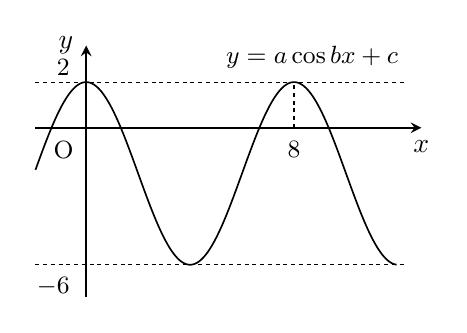
\begin{tikzpicture}[line width=0.6pt, x=0.33cm, y=0.29cm]
  \draw[dashed, dash pattern=on 1.4pt off 1.4pt, line width=0.4pt] (-1.95,2) -- (12.35,2);
  \draw[dashed, dash pattern=on 1.4pt off 1.4pt, line width=0.4pt] (-1.95,-6) -- (12.35,-6);
  \draw[dashed, dash pattern=on 1.4pt off 1.4pt, line width=0.4pt] (8,0) -- (8,2);
  \draw[->, >=stealth, line width=0.7pt] (-1.95,0) -- (12.9,0) node[below=1pt] {$x$};
  \draw[->, >=stealth, line width=0.7pt] (0,-7.4) -- (0,3.6) node[left=1pt] {$y$};
  \draw[domain=-1.95:11.95, samples=200, smooth] plot (\x, {4*cos(45*\x)-2});
  \node[anchor=south east, font=\small] at (-0.25,1.85) {$2$};
  \node[anchor=north east, font=\small] at (-0.25,-6.1) {$-6$};
  \node[anchor=north east, font=\small] at (-0.1,-0.15) {$\pt{O}$};
  \node[anchor=north, font=\small] at (8,-0.15) {$8$};
  \node[anchor=south west, font=\small] at (5.0,2.15) {$y=a\cos bx+c$};
\end{tikzpicture}
}\end{minipage}\par
\dmchoicesauto{}{$-4\pi$}{$-2\pi$}{$-\pi$}{$\pi$}{$2\pi$}
}\vspace{8mm}
\dmsection{개념 44 여러 가지 각에 대한 삼각함수의 성질}
\dmpassage{다음 삼각함수의 값을 구하시오.}
\vspace{3mm}\setcounter{dmproblemcount}{0}\dmpnum{125-01}{% id: 125-01
% book: 베이직쎈 대수 · 07 삼각함수의 그래프
% section: 개념 44 여러 가지 각에 대한 삼각함수의 성질
% passage: 다음 삼각함수의 값을 구하시오.
% figure: none
% answer: 
% answer_source: 
% variant_level: 0 (원본 전사)
% 이 파일은 build.mjs 가 items.json 에서 만든다. 고칠 때는 items.json 을 고친다.
\smash{\raisebox{4.5mm}{\dmkichul{베이직쎈 대수 125쪽 01번}}}
$\sin\dfrac{9}{4}\pi=\sin\left(2\pi+\dfrac{\pi}{4}\right)=\sin\blank=\blank$
}\vspace{8mm}
\vspace{3mm}\setcounter{dmproblemcount}{1}\dmpnum{125-02}{% id: 125-02
% book: 베이직쎈 대수 · 07 삼각함수의 그래프
% section: 개념 44 여러 가지 각에 대한 삼각함수의 성질
% passage: 다음 삼각함수의 값을 구하시오.
% figure: none
% answer: 
% answer_source: 
% variant_level: 0 (원본 전사)
% 이 파일은 build.mjs 가 items.json 에서 만든다. 고칠 때는 items.json 을 고친다.
\smash{\raisebox{4.5mm}{\dmkichul{베이직쎈 대수 125쪽 02번}}}
$\cos\dfrac{13}{6}\pi$
}\vspace{8mm}
\vspace{3mm}\setcounter{dmproblemcount}{2}\dmpnum{125-03}{% id: 125-03
% book: 베이직쎈 대수 · 07 삼각함수의 그래프
% section: 개념 44 여러 가지 각에 대한 삼각함수의 성질
% passage: 다음 삼각함수의 값을 구하시오.
% figure: none
% answer: 
% answer_source: 
% variant_level: 0 (원본 전사)
% 이 파일은 build.mjs 가 items.json 에서 만든다. 고칠 때는 items.json 을 고친다.
\smash{\raisebox{4.5mm}{\dmkichul{베이직쎈 대수 125쪽 03번}}}
$\tan\dfrac{7}{3}\pi$
}\vspace{8mm}
\vspace{3mm}\setcounter{dmproblemcount}{3}\dmpnum{125-04}{% id: 125-04
% book: 베이직쎈 대수 · 07 삼각함수의 그래프
% section: 개념 44 여러 가지 각에 대한 삼각함수의 성질
% passage: 다음 삼각함수의 값을 구하시오.
% figure: none
% answer: 
% answer_source: 
% variant_level: 0 (원본 전사)
% 이 파일은 build.mjs 가 items.json 에서 만든다. 고칠 때는 items.json 을 고친다.
\smash{\raisebox{4.5mm}{\dmkichul{베이직쎈 대수 125쪽 04번}}}
$\sin\dfrac{13}{3}\pi$
}\vspace{8mm}
\vspace{3mm}\setcounter{dmproblemcount}{4}\dmpnum{125-05}{% id: 125-05
% book: 베이직쎈 대수 · 07 삼각함수의 그래프
% section: 개념 44 여러 가지 각에 대한 삼각함수의 성질
% passage: 다음 삼각함수의 값을 구하시오.
% figure: none
% answer: 
% answer_source: 
% variant_level: 0 (원본 전사)
% 이 파일은 build.mjs 가 items.json 에서 만든다. 고칠 때는 items.json 을 고친다.
\smash{\raisebox{4.5mm}{\dmkichul{베이직쎈 대수 125쪽 05번}}}
$\tan\dfrac{17}{4}\pi$
}\vspace{8mm}
\setcounter{dmproblemcount}{5}\dmpnum{125-06}{% id: 125-06
% book: 베이직쎈 대수 · 07 삼각함수의 그래프
% section: 개념 44 여러 가지 각에 대한 삼각함수의 성질
% passage: 다음 삼각함수의 값을 구하시오.
% figure: none
% answer: 
% answer_source: 
% variant_level: 0 (원본 전사)
% 이 파일은 build.mjs 가 items.json 에서 만든다. 고칠 때는 items.json 을 고친다.
\smash{\raisebox{1.5mm}{\dmkichul{베이직쎈 대수 125쪽 06번}}}
$\cos 420^\circ$
}\vspace{8mm}
\setcounter{dmproblemcount}{6}\dmpnum{125-07}{% id: 125-07
% book: 베이직쎈 대수 · 07 삼각함수의 그래프
% section: 개념 44 여러 가지 각에 대한 삼각함수의 성질
% passage: 다음 삼각함수의 값을 구하시오.
% figure: none
% answer: 
% answer_source: 
% variant_level: 0 (원본 전사)
% 이 파일은 build.mjs 가 items.json 에서 만든다. 고칠 때는 items.json 을 고친다.
\smash{\raisebox{1.5mm}{\dmkichul{베이직쎈 대수 125쪽 07번}}}
$\sin 390^\circ$
}\vspace{8mm}
\setcounter{dmproblemcount}{7}\dmpnum{125-08}{% id: 125-08
% book: 베이직쎈 대수 · 07 삼각함수의 그래프
% section: 개념 44 여러 가지 각에 대한 삼각함수의 성질
% passage: 다음 삼각함수의 값을 구하시오.
% figure: none
% answer: 
% answer_source: 
% variant_level: 0 (원본 전사)
% 이 파일은 build.mjs 가 items.json 에서 만든다. 고칠 때는 items.json 을 고친다.
\smash{\raisebox{1.5mm}{\dmkichul{베이직쎈 대수 125쪽 08번}}}
$\cos 765^\circ$
}\vspace{8mm}
\setcounter{dmproblemcount}{8}\dmpnum{125-09}{% id: 125-09
% book: 베이직쎈 대수 · 07 삼각함수의 그래프
% section: 개념 44 여러 가지 각에 대한 삼각함수의 성질
% passage: 다음 삼각함수의 값을 구하시오.
% figure: none
% answer: 
% answer_source: 
% variant_level: 0 (원본 전사)
% 이 파일은 build.mjs 가 items.json 에서 만든다. 고칠 때는 items.json 을 고친다.
\smash{\raisebox{1.5mm}{\dmkichul{베이직쎈 대수 125쪽 09번}}}
$\tan 750^\circ$
}\vspace{8mm}
\vspace{3mm}\setcounter{dmproblemcount}{9}\dmpnum{125-10}{% id: 125-10
% book: 베이직쎈 대수 · 07 삼각함수의 그래프
% section: 개념 44 여러 가지 각에 대한 삼각함수의 성질
% passage: 다음 삼각함수의 값을 구하시오.
% figure: none
% answer: 
% answer_source: 
% variant_level: 0 (원본 전사)
% 이 파일은 build.mjs 가 items.json 에서 만든다. 고칠 때는 items.json 을 고친다.
\smash{\raisebox{4.5mm}{\dmkichul{베이직쎈 대수 125쪽 10번}}}
$\sin\left(-\dfrac{\pi}{3}\right)=-\sin\blank=\blank$
}\vspace{8mm}
\vspace{3mm}\setcounter{dmproblemcount}{10}\dmpnum{125-11}{% id: 125-11
% book: 베이직쎈 대수 · 07 삼각함수의 그래프
% section: 개념 44 여러 가지 각에 대한 삼각함수의 성질
% passage: 다음 삼각함수의 값을 구하시오.
% figure: none
% answer: 
% answer_source: 
% variant_level: 0 (원본 전사)
% 이 파일은 build.mjs 가 items.json 에서 만든다. 고칠 때는 items.json 을 고친다.
\smash{\raisebox{4.5mm}{\dmkichul{베이직쎈 대수 125쪽 11번}}}
$\cos\left(-\dfrac{\pi}{4}\right)$
}\vspace{8mm}
\vspace{3mm}\setcounter{dmproblemcount}{11}\dmpnum{125-12}{% id: 125-12
% book: 베이직쎈 대수 · 07 삼각함수의 그래프
% section: 개념 44 여러 가지 각에 대한 삼각함수의 성질
% passage: 다음 삼각함수의 값을 구하시오.
% figure: none
% answer: 
% answer_source: 
% variant_level: 0 (원본 전사)
% 이 파일은 build.mjs 가 items.json 에서 만든다. 고칠 때는 items.json 을 고친다.
\smash{\raisebox{4.5mm}{\dmkichul{베이직쎈 대수 125쪽 12번}}}
$\tan\left(-\dfrac{13}{6}\pi\right)$
}\vspace{8mm}
\vspace{3mm}\setcounter{dmproblemcount}{12}\dmpnum{125-13}{% id: 125-13
% book: 베이직쎈 대수 · 07 삼각함수의 그래프
% section: 개념 44 여러 가지 각에 대한 삼각함수의 성질
% passage: 다음 삼각함수의 값을 구하시오.
% figure: none
% answer: 
% answer_source: 
% variant_level: 0 (원본 전사)
% 이 파일은 build.mjs 가 items.json 에서 만든다. 고칠 때는 items.json 을 고친다.
\smash{\raisebox{4.5mm}{\dmkichul{베이직쎈 대수 125쪽 13번}}}
$\cos\left(-\dfrac{13}{3}\pi\right)$
}\vspace{8mm}
\vspace{3mm}\setcounter{dmproblemcount}{13}\dmpnum{125-14}{% id: 125-14
% book: 베이직쎈 대수 · 07 삼각함수의 그래프
% section: 개념 44 여러 가지 각에 대한 삼각함수의 성질
% passage: 다음 삼각함수의 값을 구하시오.
% figure: none
% answer: 
% answer_source: 
% variant_level: 0 (원본 전사)
% 이 파일은 build.mjs 가 items.json 에서 만든다. 고칠 때는 items.json 을 고친다.
\smash{\raisebox{4.5mm}{\dmkichul{베이직쎈 대수 125쪽 14번}}}
$\sin\left(-\dfrac{9}{4}\pi\right)$
}\vspace{8mm}
\setcounter{dmproblemcount}{14}\dmpnum{125-15}{% id: 125-15
% book: 베이직쎈 대수 · 07 삼각함수의 그래프
% section: 개념 44 여러 가지 각에 대한 삼각함수의 성질
% passage: 다음 삼각함수의 값을 구하시오.
% figure: none
% answer: 
% answer_source: 
% variant_level: 0 (원본 전사)
% 이 파일은 build.mjs 가 items.json 에서 만든다. 고칠 때는 items.json 을 고친다.
\smash{\raisebox{1.5mm}{\dmkichul{베이직쎈 대수 125쪽 15번}}}
$\tan (-60^\circ)$
}\vspace{8mm}
\setcounter{dmproblemcount}{15}\dmpnum{125-16}{% id: 125-16
% book: 베이직쎈 대수 · 07 삼각함수의 그래프
% section: 개념 44 여러 가지 각에 대한 삼각함수의 성질
% passage: 다음 삼각함수의 값을 구하시오.
% figure: none
% answer: 
% answer_source: 
% variant_level: 0 (원본 전사)
% 이 파일은 build.mjs 가 items.json 에서 만든다. 고칠 때는 items.json 을 고친다.
\smash{\raisebox{1.5mm}{\dmkichul{베이직쎈 대수 125쪽 16번}}}
$\cos (-750^\circ)$
}\vspace{8mm}
\setcounter{dmproblemcount}{16}\dmpnum{125-17}{% id: 125-17
% book: 베이직쎈 대수 · 07 삼각함수의 그래프
% section: 개념 44 여러 가지 각에 대한 삼각함수의 성질
% passage: 다음 삼각함수의 값을 구하시오.
% figure: none
% answer: 
% answer_source: 
% variant_level: 0 (원본 전사)
% 이 파일은 build.mjs 가 items.json 에서 만든다. 고칠 때는 items.json 을 고친다.
\smash{\raisebox{1.5mm}{\dmkichul{베이직쎈 대수 125쪽 17번}}}
$\sin (-1140^\circ)$
}\vspace{8mm}
\setcounter{dmproblemcount}{17}\dmpnum{125-18}{% id: 125-18
% book: 베이직쎈 대수 · 07 삼각함수의 그래프
% section: 개념 44 여러 가지 각에 대한 삼각함수의 성질
% passage: 다음 삼각함수의 값을 구하시오.
% figure: none
% answer: 
% answer_source: 
% variant_level: 0 (원본 전사)
% 이 파일은 build.mjs 가 items.json 에서 만든다. 고칠 때는 items.json 을 고친다.
\smash{\raisebox{1.5mm}{\dmkichul{베이직쎈 대수 125쪽 18번}}}
$\tan (-1125^\circ)$
}\vspace{8mm}
\vspace{3mm}\setcounter{dmproblemcount}{18}\dmpnum{126-19}{% id: 126-19
% book: 베이직쎈 대수 · 07 삼각함수의 그래프
% section: 개념 44 여러 가지 각에 대한 삼각함수의 성질
% figure: none
% answer: 
% answer_source: 
% variant_level: 0 (원본 전사)
% 이 파일은 build.mjs 가 items.json 에서 만든다. 고칠 때는 items.json 을 고친다.
\smash{\raisebox{4.5mm}{\dmkichul{베이직쎈 대수 126쪽 19번}}}
$\sin\dfrac{4}{3}\pi=\sin\left(\pi+\dfrac{\pi}{3}\right)=-\sin\blank=\blank$
}\vspace{8mm}
\vspace{3mm}\setcounter{dmproblemcount}{19}\dmpnum{126-20}{% id: 126-20
% book: 베이직쎈 대수 · 07 삼각함수의 그래프
% section: 개념 44 여러 가지 각에 대한 삼각함수의 성질
% passage: 다음 삼각함수의 값을 구하시오.
% figure: none
% answer: 
% answer_source: 
% variant_level: 0 (원본 전사)
% 이 파일은 build.mjs 가 items.json 에서 만든다. 고칠 때는 items.json 을 고친다.
\smash{\raisebox{4.5mm}{\dmkichul{베이직쎈 대수 126쪽 20번}}}
$\cos\dfrac{5}{6}\pi$
}\vspace{8mm}
\vspace{3mm}\setcounter{dmproblemcount}{20}\dmpnum{126-21}{% id: 126-21
% book: 베이직쎈 대수 · 07 삼각함수의 그래프
% section: 개념 44 여러 가지 각에 대한 삼각함수의 성질
% passage: 다음 삼각함수의 값을 구하시오.
% figure: none
% answer: 
% answer_source: 
% variant_level: 0 (원본 전사)
% 이 파일은 build.mjs 가 items.json 에서 만든다. 고칠 때는 items.json 을 고친다.
\smash{\raisebox{4.5mm}{\dmkichul{베이직쎈 대수 126쪽 21번}}}
$\tan\dfrac{5}{4}\pi$
}\vspace{8mm}
\setcounter{dmproblemcount}{21}\dmpnum{126-22}{% id: 126-22
% book: 베이직쎈 대수 · 07 삼각함수의 그래프
% section: 개념 44 여러 가지 각에 대한 삼각함수의 성질
% figure: none
% answer: 
% answer_source: 
% variant_level: 0 (원본 전사)
% 이 파일은 build.mjs 가 items.json 에서 만든다. 고칠 때는 items.json 을 고친다.
\smash{\raisebox{1.5mm}{\dmkichul{베이직쎈 대수 126쪽 22번}}}
$\cos 225^\circ$
}\vspace{8mm}
\setcounter{dmproblemcount}{22}\dmpnum{126-23}{% id: 126-23
% book: 베이직쎈 대수 · 07 삼각함수의 그래프
% section: 개념 44 여러 가지 각에 대한 삼각함수의 성질
% figure: none
% answer: 
% answer_source: 
% variant_level: 0 (원본 전사)
% 이 파일은 build.mjs 가 items.json 에서 만든다. 고칠 때는 items.json 을 고친다.
\smash{\raisebox{1.5mm}{\dmkichul{베이직쎈 대수 126쪽 23번}}}
$\sin 150^\circ$
}\vspace{8mm}
\setcounter{dmproblemcount}{23}\dmpnum{126-24}{% id: 126-24
% book: 베이직쎈 대수 · 07 삼각함수의 그래프
% section: 개념 44 여러 가지 각에 대한 삼각함수의 성질
% passage: 다음 삼각함수의 값을 구하시오.
% figure: none
% answer: 
% answer_source: 
% variant_level: 0 (원본 전사)
% 이 파일은 build.mjs 가 items.json 에서 만든다. 고칠 때는 items.json 을 고친다.
\smash{\raisebox{1.5mm}{\dmkichul{베이직쎈 대수 126쪽 24번}}}
$\tan 120^\circ$
}\vspace{8mm}
\vspace{3mm}\setcounter{dmproblemcount}{24}\dmpnum{126-25}{% id: 126-25
% book: 베이직쎈 대수 · 07 삼각함수의 그래프
% section: 개념 44 여러 가지 각에 대한 삼각함수의 성질
% passage: 다음 삼각함수의 값을 구하시오.
% figure: none
% answer: 
% answer_source: 
% variant_level: 0 (원본 전사)
% 이 파일은 build.mjs 가 items.json 에서 만든다. 고칠 때는 items.json 을 고친다.
\smash{\raisebox{4.5mm}{\dmkichul{베이직쎈 대수 126쪽 25번}}}
$\sin\left(\dfrac{\pi}{2}+\dfrac{\pi}{6}\right)=\cos\blank=\blank$
}\vspace{8mm}
\vspace{3mm}\setcounter{dmproblemcount}{25}\dmpnum{126-26}{% id: 126-26
% book: 베이직쎈 대수 · 07 삼각함수의 그래프
% section: 개념 44 여러 가지 각에 대한 삼각함수의 성질
% passage: 다음 삼각함수의 값을 구하시오.
% figure: none
% answer: 
% answer_source: 
% variant_level: 0 (원본 전사)
% 이 파일은 build.mjs 가 items.json 에서 만든다. 고칠 때는 items.json 을 고친다.
\smash{\raisebox{4.5mm}{\dmkichul{베이직쎈 대수 126쪽 26번}}}
$\cos\dfrac{2}{3}\pi$
}\vspace{8mm}
\vspace{3mm}\setcounter{dmproblemcount}{26}\dmpnum{126-27}{% id: 126-27
% book: 베이직쎈 대수 · 07 삼각함수의 그래프
% section: 개념 44 여러 가지 각에 대한 삼각함수의 성질
% figure: none
% answer: 
% answer_source: 
% variant_level: 0 (원본 전사)
% 이 파일은 build.mjs 가 items.json 에서 만든다. 고칠 때는 items.json 을 고친다.
\smash{\raisebox{4.5mm}{\dmkichul{베이직쎈 대수 126쪽 27번}}}
$\tan\dfrac{3}{4}\pi$
}\vspace{8mm}
\setcounter{dmproblemcount}{27}\dmpnum{126-28}{% id: 126-28
% book: 베이직쎈 대수 · 07 삼각함수의 그래프
% section: 개념 44 여러 가지 각에 대한 삼각함수의 성질
% figure: none
% answer: 
% answer_source: 
% variant_level: 0 (원본 전사)
% 이 파일은 build.mjs 가 items.json 에서 만든다. 고칠 때는 items.json 을 고친다.
\smash{\raisebox{1.5mm}{\dmkichul{베이직쎈 대수 126쪽 28번}}}
$\sin 135^\circ$
}\vspace{8mm}
\setcounter{dmproblemcount}{28}\dmpnum{126-29}{% id: 126-29
% book: 베이직쎈 대수 · 07 삼각함수의 그래프
% section: 개념 44 여러 가지 각에 대한 삼각함수의 성질
% figure: none
% answer: 
% answer_source: 
% variant_level: 0 (원본 전사)
% 이 파일은 build.mjs 가 items.json 에서 만든다. 고칠 때는 items.json 을 고친다.
\smash{\raisebox{1.5mm}{\dmkichul{베이직쎈 대수 126쪽 29번}}}
$\cos 150^\circ$
}\vspace{8mm}
\setcounter{dmproblemcount}{29}\dmpnum{126-30}{% id: 126-30
% book: 베이직쎈 대수 · 07 삼각함수의 그래프
% section: 개념 44 여러 가지 각에 대한 삼각함수의 성질
% figure: none
% answer: 
% answer_source: 
% variant_level: 0 (원본 전사)
% 이 파일은 build.mjs 가 items.json 에서 만든다. 고칠 때는 items.json 을 고친다.
\smash{\raisebox{1.5mm}{\dmkichul{베이직쎈 대수 126쪽 30번}}}
$\tan 150^\circ$
}\vspace{8mm}
\dmsection{개념 45 여러 가지 각의 삼각함수의 변형 방법}
\dmpassage{다음 식의 값을 구하시오.}
\vspace{3mm}\setcounter{dmproblemcount}{30}\dmpnum{127-31}{% id: 127-31
% book: 베이직쎈 대수 · 07 삼각함수의 그래프
% section: 개념 45 여러 가지 각의 삼각함수의 변형 방법
% passage: 다음 식의 값을 구하시오.
% figure: none
% answer: 
% answer_source: 
% variant_level: 0 (원본 전사)
% 이 파일은 build.mjs 가 items.json 에서 만든다. 고칠 때는 items.json 을 고친다.
\smash{\raisebox{4.5mm}{\dmkichul{베이직쎈 대수 127쪽 31번}}}
$\sin\left(-\dfrac{17}{6}\pi\right)+\tan\dfrac{2}{3}\pi\cos\left(-\dfrac{\pi}{6}\right)$
\dmhint{$\sin\left(-\dfrac{17}{6}\pi\right)=-\sin\blank=-\sin\left(3\pi-\blank\right)$\\ \hspace*{3em}$=-\sin\left(\dfrac{\pi}{2}\times\blank-\dfrac{\pi}{6}\right)=-\sin\blank=\blank$\\ $\tan\dfrac{2}{3}\pi=\tan\left(\pi-\blank\right)=-\tan\blank=\blank$\\ $\cos\left(-\dfrac{\pi}{6}\right)=\cos\blank=\blank$\\ $\therefore$ (주어진 식)$=\blank+(\blank)\times\blank=\blank$}
}\vspace{8mm}
\vspace{3mm}\setcounter{dmproblemcount}{31}\dmpnum{127-32}{% id: 127-32
% book: 베이직쎈 대수 · 07 삼각함수의 그래프
% section: 개념 45 여러 가지 각의 삼각함수의 변형 방법
% passage: 다음 식의 값을 구하시오.
% figure: none
% answer: 
% answer_source: 
% variant_level: 0 (원본 전사)
% 이 파일은 build.mjs 가 items.json 에서 만든다. 고칠 때는 items.json 을 고친다.
\smash{\raisebox{4.5mm}{\dmkichul{베이직쎈 대수 127쪽 32번}}}
$\sin\left(-\dfrac{11}{6}\pi\right)\cos\left(-\dfrac{21}{4}\pi\right)-\tan\dfrac{2}{3}\pi$
}\vspace{8mm}
\setcounter{dmproblemcount}{32}\dmpnum{127-33}{% id: 127-33
% book: 베이직쎈 대수 · 07 삼각함수의 그래프
% section: 개념 45 여러 가지 각의 삼각함수의 변형 방법
% passage: 다음 식의 값을 구하시오.
% figure: none
% answer: 
% answer_source: 
% variant_level: 0 (원본 전사)
% 이 파일은 build.mjs 가 items.json 에서 만든다. 고칠 때는 items.json 을 고친다.
\smash{\raisebox{1.5mm}{\dmkichul{베이직쎈 대수 127쪽 33번}}}
$\cos 135^\circ+\tan 300^\circ\sin 420^\circ$
}\vspace{8mm}
\setcounter{dmproblemcount}{33}\dmpnum{127-34}{% id: 127-34
% book: 베이직쎈 대수 · 07 삼각함수의 그래프
% section: 개념 45 여러 가지 각의 삼각함수의 변형 방법
% passage: 다음 식의 값을 구하시오.
% figure: none
% answer: 
% answer_source: 
% variant_level: 0 (원본 전사)
% 이 파일은 build.mjs 가 items.json 에서 만든다. 고칠 때는 items.json 을 고친다.
\smash{\raisebox{1.5mm}{\dmkichul{베이직쎈 대수 127쪽 34번}}}
$\sin 210^\circ+\cos 600^\circ\tan(-405^\circ)$
}\vspace{8mm}
\dmpassage{다음 식을 간단히 하시오.}
\vspace{5mm}\setcounter{dmproblemcount}{34}\dmpnum{127-35}{% id: 127-35
% book: 베이직쎈 대수 · 07 삼각함수의 그래프
% section: 개념 45 여러 가지 각의 삼각함수의 변형 방법
% passage: 다음 식을 간단히 하시오.
% figure: none
% answer: 
% answer_source: 
% variant_level: 0 (원본 전사)
% 이 파일은 build.mjs 가 items.json 에서 만든다. 고칠 때는 items.json 을 고친다.
\smash{\raisebox{6.5mm}{\dmkichul{베이직쎈 대수 127쪽 35번}}}
$\begin{aligned}\sin\left(\dfrac{\pi}{2}-\theta\right)+\cos(\pi-\theta)&=\cos\blank-\cos\blank\\ &=\blank\end{aligned}$
}\vspace{8mm}
\vspace{3mm}\setcounter{dmproblemcount}{35}\dmpnum{127-36}{% id: 127-36
% book: 베이직쎈 대수 · 07 삼각함수의 그래프
% section: 개념 45 여러 가지 각의 삼각함수의 변형 방법
% passage: 다음 식을 간단히 하시오.
% figure: none
% answer: 
% answer_source: 
% variant_level: 0 (원본 전사)
% 이 파일은 build.mjs 가 items.json 에서 만든다. 고칠 때는 items.json 을 고친다.
\smash{\raisebox{4.5mm}{\dmkichul{베이직쎈 대수 127쪽 36번}}}
$\sin(2\pi+\theta)+\cos\left(\dfrac{3}{2}\pi+\theta\right)$
}\vspace{8mm}
\vspace{3mm}\setcounter{dmproblemcount}{36}\dmpnum{127-37}{% id: 127-37
% book: 베이직쎈 대수 · 07 삼각함수의 그래프
% section: 개념 45 여러 가지 각의 삼각함수의 변형 방법
% passage: 다음 식을 간단히 하시오.
% figure: none
% answer: 
% answer_source: 
% variant_level: 0 (원본 전사)
% 이 파일은 build.mjs 가 items.json 에서 만든다. 고칠 때는 items.json 을 고친다.
\smash{\raisebox{4.5mm}{\dmkichul{베이직쎈 대수 127쪽 37번}}}
$\cos^2(\pi-\theta)+\cos^2\left(\dfrac{5}{2}\pi+\theta\right)$
}\vspace{8mm}
\vspace{3mm}\setcounter{dmproblemcount}{37}\dmpnum{127-38}{% id: 127-38
% book: 베이직쎈 대수 · 07 삼각함수의 그래프
% section: 개념 45 여러 가지 각의 삼각함수의 변형 방법
% passage: 다음 식을 간단히 하시오.
% figure: none
% answer: 
% answer_source: 
% variant_level: 0 (원본 전사)
% 이 파일은 build.mjs 가 items.json 에서 만든다. 고칠 때는 items.json 을 고친다.
\smash{\raisebox{4.5mm}{\dmkichul{베이직쎈 대수 127쪽 38번}}}
$\cos^2(2\pi+\theta)-\sin^2\left(\dfrac{3}{2}\pi-\theta\right)$
}\vspace{8mm}
\dmsection{개념 46 삼각함수표}
\dmpassage{다음 삼각함수표를 이용하여 삼각함수의 값을 구하시오.}
\begin{center}\resizebox{\ifdim\width>\linewidth\linewidth\else\width\fi}{!}{% 128-39(128쪽) — 128쪽 왼쪽 지시문(「다음 삼각함수표를 이용하여 삼각함수의 값을 구하시오.」)에 딸린 삼각함수표 일부(각 $5^\circ$~$7^\circ$).
% 스캔 표라 tabular 로 다시 조판. 칸 값은 원문 그대로.
{\setlength{\tabcolsep}{4pt}\renewcommand{\arraystretch}{1.3}%
\begin{tabular}{|c|c|c|c|}
\hline
\makebox[11mm]{$x$} & \makebox[16mm]{$\sin x$} & \makebox[16mm]{$\cos x$} & \makebox[16mm]{$\tan x$} \\
\hline
$5^\circ$ & $0.0872$ & $0.9962$ & $0.0875$ \\
\hline
$6^\circ$ & $0.1045$ & $0.9945$ & $0.1051$ \\
\hline
$7^\circ$ & $0.1219$ & $0.9925$ & $0.1228$ \\
\hline
\end{tabular}}
}\end{center}\vspace{4mm}
\setcounter{dmproblemcount}{38}\dmpnum{128-39}{% id: 128-39
% book: 베이직쎈 대수 · 07 삼각함수의 그래프
% section: 개념 46 삼각함수표
% passage: 다음 삼각함수표를 이용하여 삼각함수의 값을 구하시오.
% figure: tikz:fig-128-39
% answer: 
% answer_source: 
% variant_level: 0 (원본 전사)
% 이 파일은 build.mjs 가 items.json 에서 만든다. 고칠 때는 items.json 을 고친다.
\smash{\raisebox{1.5mm}{\dmkichul{베이직쎈 대수 128쪽 39번}}}
$\sin 365^\circ$
}\vspace{8mm}
\setcounter{dmproblemcount}{39}\dmpnum{128-40}{% id: 128-40
% book: 베이직쎈 대수 · 07 삼각함수의 그래프
% section: 개념 46 삼각함수표
% passage: 다음 삼각함수표를 이용하여 삼각함수의 값을 구하시오.
% figure: tikz:fig-128-39
% answer: 
% answer_source: 
% variant_level: 0 (원본 전사)
% 이 파일은 build.mjs 가 items.json 에서 만든다. 고칠 때는 items.json 을 고친다.
\smash{\raisebox{1.5mm}{\dmkichul{베이직쎈 대수 128쪽 40번}}}
$\cos 174^\circ$
}\vspace{8mm}
\setcounter{dmproblemcount}{40}\dmpnum{128-41}{% id: 128-41
% book: 베이직쎈 대수 · 07 삼각함수의 그래프
% section: 개념 46 삼각함수표
% passage: 다음 삼각함수표를 이용하여 삼각함수의 값을 구하시오.
% figure: tikz:fig-128-39
% answer: 
% answer_source: 
% variant_level: 0 (원본 전사)
% 이 파일은 build.mjs 가 items.json 에서 만든다. 고칠 때는 items.json 을 고친다.
\smash{\raisebox{1.5mm}{\dmkichul{베이직쎈 대수 128쪽 41번}}}
$\tan 185^\circ$
}\vspace{8mm}
\setcounter{dmproblemcount}{41}\dmpnum{128-42}{% id: 128-42
% book: 베이직쎈 대수 · 07 삼각함수의 그래프
% section: 개념 46 삼각함수표
% passage: 다음 삼각함수표를 이용하여 삼각함수의 값을 구하시오.
% figure: tikz:fig-128-39
% answer: 
% answer_source: 
% variant_level: 0 (원본 전사)
% 이 파일은 build.mjs 가 items.json 에서 만든다. 고칠 때는 items.json 을 고친다.
\smash{\raisebox{1.5mm}{\dmkichul{베이직쎈 대수 128쪽 42번}}}
$\sin 353^\circ$
}\vspace{8mm}
\setcounter{dmproblemcount}{42}\dmpnum{128-43}{% id: 128-43
% book: 베이직쎈 대수 · 07 삼각함수의 그래프
% section: 개념 46 삼각함수표
% passage: 다음 삼각함수표를 이용하여 삼각함수의 값을 구하시오.
% figure: tikz:fig-128-39
% answer: 
% answer_source: 
% variant_level: 0 (원본 전사)
% 이 파일은 build.mjs 가 items.json 에서 만든다. 고칠 때는 items.json 을 고친다.
\smash{\raisebox{1.5mm}{\dmkichul{베이직쎈 대수 128쪽 43번}}}
$\cos 96^\circ$
}\vspace{8mm}
\dmpassage{다음 삼각함수표를 이용하여 삼각함수의 값을 구하시오.}
\begin{center}\resizebox{\ifdim\width>\linewidth\linewidth\else\width\fi}{!}{% 128-44(128쪽) — 128쪽 오른쪽 지시문(「다음 삼각함수표를 이용하여 삼각함수의 값을 구하시오.」)에 딸린 삼각함수표 일부(각 $31^\circ$~$33^\circ$).
% 스캔 표라 tabular 로 다시 조판. 칸 값은 원문 그대로.
{\setlength{\tabcolsep}{4pt}\renewcommand{\arraystretch}{1.3}%
\begin{tabular}{|c|c|c|c|}
\hline
\makebox[11mm]{$x$} & \makebox[16mm]{$\sin x$} & \makebox[16mm]{$\cos x$} & \makebox[16mm]{$\tan x$} \\
\hline
$31^\circ$ & $0.5150$ & $0.8572$ & $0.6009$ \\
\hline
$32^\circ$ & $0.5299$ & $0.8480$ & $0.6249$ \\
\hline
$33^\circ$ & $0.5446$ & $0.8387$ & $0.6494$ \\
\hline
\end{tabular}}
}\end{center}\vspace{4mm}
\setcounter{dmproblemcount}{43}\dmpnum{128-44}{% id: 128-44
% book: 베이직쎈 대수 · 07 삼각함수의 그래프
% section: 개념 46 삼각함수표
% passage: 다음 삼각함수표를 이용하여 삼각함수의 값을 구하시오.
% figure: tikz:fig-128-44
% answer: 
% answer_source: 
% variant_level: 0 (원본 전사)
% 이 파일은 build.mjs 가 items.json 에서 만든다. 고칠 때는 items.json 을 고친다.
\smash{\raisebox{1.5mm}{\dmkichul{베이직쎈 대수 128쪽 44번}}}
$\sin 753^\circ$
}\vspace{8mm}
\setcounter{dmproblemcount}{44}\dmpnum{128-45}{% id: 128-45
% book: 베이직쎈 대수 · 07 삼각함수의 그래프
% section: 개념 46 삼각함수표
% passage: 다음 삼각함수표를 이용하여 삼각함수의 값을 구하시오.
% figure: tikz:fig-128-44
% answer: 
% answer_source: 
% variant_level: 0 (원본 전사)
% 이 파일은 build.mjs 가 items.json 에서 만든다. 고칠 때는 items.json 을 고친다.
\smash{\raisebox{1.5mm}{\dmkichul{베이직쎈 대수 128쪽 45번}}}
$\tan 211^\circ$
}\vspace{8mm}
\setcounter{dmproblemcount}{45}\dmpnum{128-46}{% id: 128-46
% book: 베이직쎈 대수 · 07 삼각함수의 그래프
% section: 개념 46 삼각함수표
% passage: 다음 삼각함수표를 이용하여 삼각함수의 값을 구하시오.
% figure: tikz:fig-128-44
% answer: 
% answer_source: 
% variant_level: 0 (원본 전사)
% 이 파일은 build.mjs 가 items.json 에서 만든다. 고칠 때는 items.json 을 고친다.
\smash{\raisebox{1.5mm}{\dmkichul{베이직쎈 대수 128쪽 46번}}}
$\sin 122^\circ$
}\vspace{8mm}
\setcounter{dmproblemcount}{46}\dmpnum{128-47}{% id: 128-47
% book: 베이직쎈 대수 · 07 삼각함수의 그래프
% section: 개념 46 삼각함수표
% passage: 다음 삼각함수표를 이용하여 삼각함수의 값을 구하시오.
% figure: tikz:fig-128-44
% answer: 
% answer_source: 
% variant_level: 0 (원본 전사)
% 이 파일은 build.mjs 가 items.json 에서 만든다. 고칠 때는 items.json 을 고친다.
\smash{\raisebox{1.5mm}{\dmkichul{베이직쎈 대수 128쪽 47번}}}
$\cos 147^\circ$
}\vspace{8mm}
\setcounter{dmproblemcount}{47}\dmpnum{128-48}{% id: 128-48
% book: 베이직쎈 대수 · 07 삼각함수의 그래프
% section: 개념 46 삼각함수표
% passage: 다음 삼각함수표를 이용하여 삼각함수의 값을 구하시오.
% figure: tikz:fig-128-44
% answer: 
% answer_source: 
% variant_level: 0 (원본 전사)
% 이 파일은 build.mjs 가 items.json 에서 만든다. 고칠 때는 items.json 을 고친다.
\smash{\raisebox{1.5mm}{\dmkichul{베이직쎈 대수 128쪽 48번}}}
$\tan 392^\circ$
}\vspace{8mm}
\dmsection{개념 47 삼각방정식}
\dmpassage{다음 방정식을 푸시오.}
\vspace{3mm}\setcounter{dmproblemcount}{48}\dmpnum{129-49}{% id: 129-49
% book: 베이직쎈 대수 · 07 삼각함수의 그래프
% section: 개념 47 삼각방정식
% passage: 다음 방정식을 푸시오.
% figure: none
% answer: 
% answer_source: 
% variant_level: 0 (원본 전사)
% 이 파일은 build.mjs 가 items.json 에서 만든다. 고칠 때는 items.json 을 고친다.
\smash{\raisebox{4.5mm}{\dmkichul{베이직쎈 대수 129쪽 49번}}}
$\sin x=\dfrac{1}{2}$ \dmcondfill{$0\le x<2\pi$}{}
\dmhint{주어진 방정식의 해는 함수 $y=\sin x\ (0\le x<2\pi)$의 그래프와 직선 $y=\blank$의 교점의 $x$좌표와 같다.\par\smallskip\dispeq{% 129-49(129쪽) — 🎯 힌트 안 그래프: $y=\sin x$ $(0\le x<2\pi)$ 의 그래프와 직선 $y=\frac{1}{2}$.
% 스캔 화질이 낮아 TikZ 로 다시 그림. 라벨은 원문에 있는 것만 — $y$축 $1$·$-1$, $x$축 $\frac{\pi}{2}$·$\pi$·$\frac{3}{2}\pi$·$2\pi$.
% 교점의 $x$좌표(= 이 문항의 답)는 원문에도 적혀 있지 않으므로 점만 찍고 값은 쓰지 않는다.
\begin{tikzpicture}[line width=0.6pt, x=0.80cm, y=0.72cm]
  \draw[dotted, line width=0.5pt] (0,1) -- (1.5708,1) (1.5708,0) -- (1.5708,1);
  \draw[dotted, line width=0.5pt] (0,-1) -- (4.7124,-1) (4.7124,0) -- (4.7124,-1);
  \draw[dotted, line width=0.5pt] (6.2832,0) -- (6.2832,0.5);
  \draw[->, >=stealth, line width=0.7pt] (-0.65,0) -- (7.45,0) node[below=1pt, font=\footnotesize] {$x$};
  \draw[->, >=stealth, line width=0.7pt] (0,-1.70) -- (0,1.80) node[left=1pt, font=\footnotesize] {$y$};
  \draw[line width=0.6pt] (-0.65,0.5) -- (7.05,0.5);
  \draw[line width=0.7pt, domain=0:6.2832, samples=140, smooth] plot (\x, {sin(57.2958*\x)});
  \fill (0,0) circle (1.7pt);
  \draw[fill=white, line width=0.5pt] (6.2832,0) circle (1.7pt);
  \fill[red!75] (0.5236,0.5) circle (1.7pt);
  \fill[red!75] (2.6180,0.5) circle (1.7pt);
  \node[anchor=east, font=\footnotesize] at (-0.12,1) {$1$};
  \node[anchor=east, font=\footnotesize] at (-0.12,-1) {$-1$};
  \node[anchor=north east, font=\footnotesize] at (-0.04,-0.06) {$\pt{O}$};
  \node[anchor=north, font=\footnotesize] at (1.5708,-0.10) {$\dfrac{\pi}{2}$};
  \node[anchor=south, font=\footnotesize, fill=white, inner sep=0.6pt] at (3.1416,0.05) {$\pi$};
  \node[anchor=north west, font=\footnotesize] at (5.00,-0.52) {$\dfrac{3}{2}\pi$};
  \draw[->, >=stealth, line width=0.4pt] (5.00,-0.56) -- (4.77,-0.10);
  \node[anchor=south east, font=\footnotesize, fill=white, inner sep=0.6pt] at (6.55,0.05) {$2\pi$};
  \node[anchor=south west, font=\footnotesize] at (0.95,1.04) {$y=\sin x$};
  \node[anchor=south east, font=\footnotesize] at (7.00,0.56) {$y=\dfrac{1}{2}$};
\end{tikzpicture}
}\par\smallskip\noindent 따라서 구하는 해는 \quad $x=\blank$ 또는 $x=\blank[2.4em]$}
}\vspace{8mm}
\vspace{3mm}\setcounter{dmproblemcount}{49}\dmpnum{129-50}{% id: 129-50
% book: 베이직쎈 대수 · 07 삼각함수의 그래프
% section: 개념 47 삼각방정식
% passage: 다음 방정식을 푸시오.
% figure: none
% answer: 
% answer_source: 
% variant_level: 0 (원본 전사)
% 이 파일은 build.mjs 가 items.json 에서 만든다. 고칠 때는 items.json 을 고친다.
\smash{\raisebox{4.5mm}{\dmkichul{베이직쎈 대수 129쪽 50번}}}
$\cos x=\dfrac{\sqrt{3}}{2}$ \dmcondfill{$0\le x<2\pi$}{}
}\vspace{8mm}
\vspace{3mm}\setcounter{dmproblemcount}{50}\dmpnum{129-51}{% id: 129-51
% book: 베이직쎈 대수 · 07 삼각함수의 그래프
% section: 개념 47 삼각방정식
% passage: 다음 방정식을 푸시오.
% figure: none
% answer: 
% answer_source: 
% variant_level: 0 (원본 전사)
% 이 파일은 build.mjs 가 items.json 에서 만든다. 고칠 때는 items.json 을 고친다.
\smash{\raisebox{4.5mm}{\dmkichul{베이직쎈 대수 129쪽 51번}}}
$\cos x=-\dfrac{1}{2}$ \dmcondfill{$0\le x<2\pi$}{}
}\vspace{8mm}
\setcounter{dmproblemcount}{51}\dmpnum{129-52}{% id: 129-52
% book: 베이직쎈 대수 · 07 삼각함수의 그래프
% section: 개념 47 삼각방정식
% passage: 다음 방정식을 푸시오.
% figure: none
% answer: 
% answer_source: 
% variant_level: 0 (원본 전사)
% 이 파일은 build.mjs 가 items.json 에서 만든다. 고칠 때는 items.json 을 고친다.
\smash{\raisebox{1.5mm}{\dmkichul{베이직쎈 대수 129쪽 52번}}}
$\tan x=1$ \dmcondfill{$0\le x<2\pi$}{}
}\vspace{8mm}
\vspace{3mm}\setcounter{dmproblemcount}{52}\dmpnum{129-53}{% id: 129-53
% book: 베이직쎈 대수 · 07 삼각함수의 그래프
% section: 개념 47 삼각방정식
% passage: 다음 방정식을 푸시오.
% figure: none
% answer: 
% answer_source: 
% variant_level: 0 (원본 전사)
% 이 파일은 build.mjs 가 items.json 에서 만든다. 고칠 때는 items.json 을 고친다.
\smash{\raisebox{4.5mm}{\dmkichul{베이직쎈 대수 129쪽 53번}}}
$\tan x=\dfrac{\sqrt{3}}{3}$ \dmcondfill{$0\le x<2\pi$}{}
}\vspace{8mm}
\vspace{3mm}\setcounter{dmproblemcount}{53}\dmpnum{129-54}{% id: 129-54
% book: 베이직쎈 대수 · 07 삼각함수의 그래프
% section: 개념 47 삼각방정식
% passage: 다음 방정식을 푸시오.
% figure: none
% answer: 
% answer_source: 
% variant_level: 0 (원본 전사)
% 이 파일은 build.mjs 가 items.json 에서 만든다. 고칠 때는 items.json 을 고친다.
\smash{\raisebox{4.5mm}{\dmkichul{베이직쎈 대수 129쪽 54번}}}
$\sin\left(2x-\dfrac{\pi}{4}\right)=\dfrac{\sqrt{2}}{2}$ \dmcondfill{$0\le x<\pi$}{}
\dmhint{$2x-\dfrac{\pi}{4}=\theta$로 놓으면 \quad $\blank\le\theta<\blank$\\ 주어진 방정식은 \quad $\sin\theta=\dfrac{\sqrt{2}}{2}$\par\smallskip\dispeq{% 129-54(129쪽) — 🎯 힌트 안 그래프: $\theta=2x-\frac{\pi}{4}$ 로 놓았을 때 $y=\sin\theta$ $\left(-\frac{\pi}{4}\le\theta<\frac{7}{4}\pi\right)$ 와 직선 $y=\frac{\sqrt{2}}{2}$.
% 스캔 화질이 낮아 TikZ 로 다시 그림. 라벨은 원문에 있는 것만 — $1$·$-1$, $-\frac{\pi}{4}$·$\frac{\pi}{2}$·$\pi$·$\frac{3}{2}\pi$·$\frac{7}{4}\pi$.
% 교점의 $\theta$ 값(답으로 이어지는 값)은 원문에도 없으므로 점만 찍는다. 왼쪽 끝은 닫힌 점, 오른쪽 끝은 열린 점.
\begin{tikzpicture}[line width=0.6pt, x=0.80cm, y=0.72cm]
  \draw[dotted, line width=0.5pt] (0,1) -- (1.5708,1) (1.5708,0) -- (1.5708,1);
  \draw[dotted, line width=0.5pt] (0,-1) -- (4.7124,-1) (4.7124,0) -- (4.7124,-1);
  \draw[->, >=stealth, line width=0.7pt] (-1.95,0) -- (6.55,0) node[below=1pt, font=\footnotesize] {$\theta$};
  \draw[->, >=stealth, line width=0.7pt] (0,-1.70) -- (0,1.80) node[left=1pt, font=\footnotesize] {$y$};
  \draw[line width=0.6pt] (-1.95,0.7071) -- (6.20,0.7071);
  \draw[line width=0.7pt, domain=-0.7854:5.4978, samples=140, smooth] plot (\x, {sin(57.2958*\x)});
  \fill (-0.7854,-0.7071) circle (1.7pt);
  \draw[fill=white, line width=0.5pt] (5.4978,-0.7071) circle (1.7pt);
  \fill[red!75] (0.7854,0.7071) circle (1.7pt);
  \fill[red!75] (2.3562,0.7071) circle (1.7pt);
  \node[anchor=east, font=\footnotesize] at (-0.12,1) {$1$};
  \node[anchor=east, font=\footnotesize] at (-0.12,-1) {$-1$};
  \node[anchor=south east, font=\footnotesize] at (-0.10,0.04) {$-\dfrac{\pi}{4}$};
  \node[anchor=north, font=\footnotesize] at (0.18,-0.06) {$\pt{O}$};
  \node[anchor=north, font=\footnotesize] at (1.5708,-0.10) {$\dfrac{\pi}{2}$};
  \node[anchor=south, font=\footnotesize, fill=white, inner sep=0.6pt] at (3.1416,0.05) {$\pi$};
  \node[anchor=south, font=\footnotesize, fill=white, inner sep=0.6pt] at (4.7124,0.05) {$\dfrac{3}{2}\pi$};
  \node[anchor=north west, font=\footnotesize] at (5.62,-0.30) {$\dfrac{7}{4}\pi$};
  \draw[->, >=stealth, line width=0.4pt] (5.62,-0.34) -- (5.45,-0.62);
  \node[anchor=south west, font=\footnotesize] at (1.00,1.04) {$y=\sin\theta$};
  \node[anchor=south east, font=\footnotesize] at (6.18,0.76) {$y=\dfrac{\sqrt{2}}{2}$};
\end{tikzpicture}
}\par\smallskip\noindent $\sin\theta=\dfrac{\sqrt{2}}{2}$의 해를 구하면 \quad $\theta=\blank$ 또는 $\theta=\blank[2.4em]$\\ 즉 $2x-\dfrac{\pi}{4}=\blank$ 또는 $2x-\dfrac{\pi}{4}=\blank[2.4em]$이므로\\ \hspace*{1.5em}$x=\blank$ 또는 $x=\blank$}
}\vspace{8mm}
\setcounter{dmproblemcount}{54}\dmpnum{129-55}{% id: 129-55
% book: 베이직쎈 대수 · 07 삼각함수의 그래프
% section: 개념 47 삼각방정식
% passage: 다음 방정식을 푸시오.
% figure: none
% answer: 
% answer_source: 
% variant_level: 0 (원본 전사)
% 이 파일은 build.mjs 가 items.json 에서 만든다. 고칠 때는 items.json 을 고친다.
\smash{\raisebox{1.5mm}{\dmkichul{베이직쎈 대수 129쪽 55번}}}
$2\cos 2x=1$ \dmcondfill{$0\le x<\pi$}{}
}\vspace{8mm}
\vspace{3mm}\setcounter{dmproblemcount}{55}\dmpnum{129-56}{% id: 129-56
% book: 베이직쎈 대수 · 07 삼각함수의 그래프
% section: 개념 47 삼각방정식
% passage: 다음 방정식을 푸시오.
% figure: none
% answer: 
% answer_source: 
% variant_level: 0 (원본 전사)
% 이 파일은 build.mjs 가 items.json 에서 만든다. 고칠 때는 items.json 을 고친다.
\smash{\raisebox{4.5mm}{\dmkichul{베이직쎈 대수 129쪽 56번}}}
$\tan\left(x+\dfrac{\pi}{2}\right)=\sqrt{3}$ \dmcondfill{$-\dfrac{\pi}{2}\le x<\dfrac{3}{2}\pi$}{}
}\vspace{8mm}
\dmsection{개념 48 삼각부등식}
\dmpassage{다음 부등식을 푸시오.}
\vspace{3mm}\setcounter{dmproblemcount}{56}\dmpnum{130-57}{% id: 130-57
% book: 베이직쎈 대수 · 07 삼각함수의 그래프
% section: 개념 48 삼각부등식
% passage: 다음 부등식을 푸시오.
% figure: none
% answer: 
% answer_source: 
% variant_level: 0 (원본 전사)
% 이 파일은 build.mjs 가 items.json 에서 만든다. 고칠 때는 items.json 을 고친다.
\smash{\raisebox{4.5mm}{\dmkichul{베이직쎈 대수 130쪽 57번}}}
$\cos x\le-\dfrac{\sqrt{3}}{2}$ \dmcondfill{$0\le x<2\pi$}{}
\dmhint{주어진 부등식의 해는 함수 $y=\cos x\ (0\le x<2\pi)$의 그래프가 직선 $y=\blank$과 만나는 부분 또는 직선보다 아래쪽에 있는 부분의 $x$의 값의 범위이다.\par\smallskip\dispeq{% 130-57(130쪽) — 🎯 힌트 안 그래프: $y=\cos x$ $(0\le x<2\pi)$ 의 그래프와 직선 $y=-\frac{\sqrt{3}}{2}$.
% 스캔 화질이 낮아 TikZ 로 다시 그림. 라벨은 원문에 있는 것만 — $1$·$-1$, $\frac{\pi}{2}$·$\pi$·$\frac{3}{2}\pi$·$2\pi$.
% 원문처럼 직선보다 아래쪽에 있는 곡선 부분만 색을 넣었고, 그 양 끝 $x$좌표(= 답)는 원문에도 적혀 있지 않으므로 쓰지 않는다.
% $\frac{\pi}{2}$·$\frac{3}{2}\pi$ 는 곡선을 피해 원문처럼 아래쪽에 두고 가는 지시선으로 축의 자리를 가리킨다.
\begin{tikzpicture}[line width=0.6pt, x=0.80cm, y=0.72cm]
  \draw[dotted, line width=0.5pt] (0,1) -- (6.2832,1) (6.2832,0) -- (6.2832,1);
  \draw[dotted, line width=0.5pt] (0,-1) -- (4.7124,-1) (3.1416,0) -- (3.1416,-1);
  \draw[->, >=stealth, line width=0.7pt] (-0.65,0) -- (7.45,0) node[above=1pt, font=\footnotesize] {$x$};
  \draw[->, >=stealth, line width=0.7pt] (0,-1.90) -- (0,1.80) node[left=1pt, font=\footnotesize] {$y$};
  \draw[line width=0.6pt] (-0.65,-0.8660) -- (7.05,-0.8660);
  \draw[line width=0.7pt, domain=0:6.2832, samples=140, smooth] plot (\x, {cos(57.2958*\x)});
  \draw[red!75, line width=0.9pt, domain=2.6180:3.6652, samples=60, smooth] plot (\x, {cos(57.2958*\x)});
  \fill (0,1) circle (1.7pt);
  \draw[fill=white, line width=0.5pt] (6.2832,1) circle (1.7pt);
  \fill[red!75] (2.6180,-0.8660) circle (1.7pt);
  \fill[red!75] (3.6652,-0.8660) circle (1.7pt);
  \node[anchor=east, font=\footnotesize] at (-0.12,1) {$1$};
  \node[anchor=east, font=\footnotesize] at (-0.12,-1) {$-1$};
  \node[anchor=north east, font=\footnotesize] at (-0.04,-0.06) {$\pt{O}$};
  \node[anchor=south, font=\footnotesize, fill=white, inner sep=0.6pt] at (3.1416,0.05) {$\pi$};
  \node[anchor=north, font=\footnotesize] at (1.24,-1.30) {$\dfrac{\pi}{2}$};
  \draw[line width=0.4pt] (1.5708,-0.08) to[out=250, in=60] (1.30,-1.28);
  \node[anchor=north, font=\footnotesize] at (5.05,-1.30) {$\dfrac{3}{2}\pi$};
  \draw[line width=0.4pt] (4.7124,-0.08) to[out=290, in=120] (4.99,-1.28);
  \node[anchor=north, font=\footnotesize] at (6.2832,-0.10) {$2\pi$};
  \node[anchor=south east, font=\footnotesize] at (6.15,1.04) {$y=\cos x$};
  \node[anchor=west, font=\footnotesize] at (7.10,-0.8660) {$y=-\dfrac{\sqrt{3}}{2}$};
\end{tikzpicture}
}\par\smallskip\noindent 따라서 구하는 해는 \quad $\blank\le x\le\blank$}
}\vspace{8mm}
\vspace{3mm}\setcounter{dmproblemcount}{57}\dmpnum{130-58}{% id: 130-58
% book: 베이직쎈 대수 · 07 삼각함수의 그래프
% section: 개념 48 삼각부등식
% passage: 다음 부등식을 푸시오.
% figure: none
% answer: 
% answer_source: 
% variant_level: 0 (원본 전사)
% 이 파일은 build.mjs 가 items.json 에서 만든다. 고칠 때는 items.json 을 고친다.
\smash{\raisebox{4.5mm}{\dmkichul{베이직쎈 대수 130쪽 58번}}}
$\sin x>\dfrac{\sqrt{2}}{2}$ \dmcondfill{$0\le x<2\pi$}{}
}\vspace{8mm}
\vspace{3mm}\setcounter{dmproblemcount}{58}\dmpnum{130-59}{% id: 130-59
% book: 베이직쎈 대수 · 07 삼각함수의 그래프
% section: 개념 48 삼각부등식
% passage: 다음 부등식을 푸시오.
% figure: none
% answer: 
% answer_source: 
% variant_level: 0 (원본 전사)
% 이 파일은 build.mjs 가 items.json 에서 만든다. 고칠 때는 items.json 을 고친다.
\smash{\raisebox{4.5mm}{\dmkichul{베이직쎈 대수 130쪽 59번}}}
$\cos x<\dfrac{1}{2}$ \dmcondfill{$0\le x<2\pi$}{}
}\vspace{8mm}
\setcounter{dmproblemcount}{59}\dmpnum{130-60}{% id: 130-60
% book: 베이직쎈 대수 · 07 삼각함수의 그래프
% section: 개념 48 삼각부등식
% passage: 다음 부등식을 푸시오.
% figure: none
% answer: 
% answer_source: 
% variant_level: 0 (원본 전사)
% 이 파일은 build.mjs 가 items.json 에서 만든다. 고칠 때는 items.json 을 고친다.
\smash{\raisebox{1.5mm}{\dmkichul{베이직쎈 대수 130쪽 60번}}}
$\tan x\ge-1$ \dmcondfill{$0\le x<2\pi$}{}
}\vspace{8mm}
\vspace{3mm}\setcounter{dmproblemcount}{60}\dmpnum{130-61}{% id: 130-61
% book: 베이직쎈 대수 · 07 삼각함수의 그래프
% section: 개념 48 삼각부등식
% passage: 다음 부등식을 푸시오.
% figure: none
% answer: 
% answer_source: 
% variant_level: 0 (원본 전사)
% 이 파일은 build.mjs 가 items.json 에서 만든다. 고칠 때는 items.json 을 고친다.
\smash{\raisebox{4.5mm}{\dmkichul{베이직쎈 대수 130쪽 61번}}}
$\sqrt{3}\tan x<1$ \dmcondfill{$0\le x<2\pi$}{}
}\vspace{8mm}
\vspace{3mm}\setcounter{dmproblemcount}{61}\dmpnum{130-62}{% id: 130-62
% book: 베이직쎈 대수 · 07 삼각함수의 그래프
% section: 개념 48 삼각부등식
% passage: 다음 부등식을 푸시오.
% figure: none
% answer: 
% answer_source: 
% variant_level: 0 (원본 전사)
% 이 파일은 build.mjs 가 items.json 에서 만든다. 고칠 때는 items.json 을 고친다.
\smash{\raisebox{4.5mm}{\dmkichul{베이직쎈 대수 130쪽 62번}}}
$\cos\left(x-\dfrac{\pi}{3}\right)\le-\dfrac{1}{2}$ \dmcondfill{$0\le x<2\pi$}{}
\dmhint{$x-\dfrac{\pi}{3}=\theta$로 놓으면 \quad $\blank\le\theta<\blank$\\ 주어진 부등식은 \quad $\cos\theta\le-\dfrac{1}{2}$\par\smallskip\dispeq{% 130-62(130쪽) — 🎯 힌트 안 그래프: $\theta=x-\frac{\pi}{3}$ 로 놓았을 때 $y=\cos\theta$ $\left(-\frac{\pi}{3}\le\theta<\frac{5}{3}\pi\right)$ 와 직선 $y=-\frac{1}{2}$.
% 스캔 화질이 낮아 TikZ 로 다시 그림. 라벨은 원문에 있는 것만 — $1$·$-1$, $-\frac{\pi}{3}$·$\pi$·$\frac{5}{3}\pi$.
% 원문처럼 직선보다 아래쪽 곡선 부분만 색을 넣었고 그 양 끝 값(답으로 이어지는 값)은 적지 않는다. 왼쪽 끝 닫힌 점·오른쪽 끝 열린 점.
\begin{tikzpicture}[line width=0.6pt, x=0.80cm, y=0.72cm]
  \draw[dotted, line width=0.5pt] (0,-1) -- (3.1416,-1) (3.1416,-0.5) -- (3.1416,-1);
  \draw[->, >=stealth, line width=0.7pt] (-1.65,0) -- (6.45,0) node[above=1pt, font=\footnotesize] {$\theta$};
  \draw[->, >=stealth, line width=0.7pt] (0,-1.70) -- (0,1.80) node[left=1pt, font=\footnotesize] {$y$};
  \draw[line width=0.6pt] (-1.65,-0.5) -- (5.95,-0.5);
  \draw[line width=0.7pt, domain=-1.0472:5.2360, samples=140, smooth] plot (\x, {cos(57.2958*\x)});
  \draw[red!75, line width=0.9pt, domain=2.0944:4.1888, samples=60, smooth] plot (\x, {cos(57.2958*\x)});
  \fill (-1.0472,0.5) circle (1.7pt);
  \draw[fill=white, line width=0.5pt] (5.2360,0.5) circle (1.7pt);
  \fill[red!75] (2.0944,-0.5) circle (1.7pt);
  \fill[red!75] (4.1888,-0.5) circle (1.7pt);
  \node[anchor=east, font=\footnotesize] at (-0.12,1) {$1$};
  \node[anchor=east, font=\footnotesize] at (-0.12,-1) {$-1$};
  \node[anchor=east, font=\footnotesize] at (-1.40,0.52) {$-\dfrac{\pi}{3}$};
  \draw[->, >=stealth, line width=0.4pt] (-1.36,0.46) -- (-1.12,0.46);
  \node[anchor=north east, font=\footnotesize] at (-0.06,-0.06) {$\pt{O}$};
  \node[anchor=south, font=\footnotesize, fill=white, inner sep=0.6pt] at (3.1416,0.05) {$\pi$};
  \node[anchor=south, font=\footnotesize] at (5.42,0.62) {$\dfrac{5}{3}\pi$};
  \draw[->, >=stealth, line width=0.4pt] (5.42,0.58) -- (5.28,0.42);
  \node[anchor=north, font=\footnotesize] at (2.70,-1.06) {$y=\cos\theta$};
  \node[anchor=west, font=\footnotesize] at (6.00,-0.5) {$y=-\dfrac{1}{2}$};
\end{tikzpicture}
}\par\smallskip\noindent $\cos\theta\le-\dfrac{1}{2}$의 해를 구하면 \quad $\blank\le\theta\le\blank$\\ 즉 $\blank\le x-\dfrac{\pi}{3}\le\blank$이므로 \quad $\blank\le x\le\blank$}
}\vspace{8mm}
\vspace{3mm}\setcounter{dmproblemcount}{62}\dmpnum{130-63}{% id: 130-63
% book: 베이직쎈 대수 · 07 삼각함수의 그래프
% section: 개념 48 삼각부등식
% passage: 다음 부등식을 푸시오.
% figure: none
% answer: 
% answer_source: 
% variant_level: 0 (원본 전사)
% 이 파일은 build.mjs 가 items.json 에서 만든다. 고칠 때는 items.json 을 고친다.
\smash{\raisebox{4.5mm}{\dmkichul{베이직쎈 대수 130쪽 63번}}}
$\sin\left(x+\dfrac{\pi}{3}\right)\le\dfrac{1}{2}$ \dmcondfill{$0\le x<2\pi$}{}
}\vspace{8mm}
\vspace{3mm}\setcounter{dmproblemcount}{63}\dmpnum{130-64}{% id: 130-64
% book: 베이직쎈 대수 · 07 삼각함수의 그래프
% section: 개념 48 삼각부등식
% passage: 다음 부등식을 푸시오.
% figure: none
% answer: 
% answer_source: 
% variant_level: 0 (원본 전사)
% 이 파일은 build.mjs 가 items.json 에서 만든다. 고칠 때는 items.json 을 고친다.
\smash{\raisebox{4.5mm}{\dmkichul{베이직쎈 대수 130쪽 64번}}}
$\tan\left(x-\dfrac{\pi}{6}\right)>1$ \dmcondfill{$0\le x<\pi$}{}
}\vspace{8mm}
\dmsection{유형 073 여러 가지 각에 대한 삼각함수의 성질}
\vspace{3mm}\setcounter{dmproblemcount}{0}\dmpnum{131-01}{% id: 131-01
% book: 베이직쎈 대수 · 07 삼각함수의 그래프
% section: 유형 073 여러 가지 각에 대한 삼각함수의 성질
% figure: none
% answer: 
% answer_source: 
% variant_level: 0 (원본 전사)
% 이 파일은 build.mjs 가 items.json 에서 만든다. 고칠 때는 items.json 을 고친다.
\smash{\raisebox{4.5mm}{\dmkichul{베이직쎈 대수 131쪽 01번}}}
$\dfrac{\cos(2\pi-\theta)}{\cos(\pi+\theta)}-\dfrac{\cos\left(\frac{3}{2}\pi+\theta\right)}{\sin(\pi-\theta)}$를 간단히 하시오.
}\vspace{8mm}
\setcounter{dmproblemcount}{1}\dmpnum{131-02}{% id: 131-02
% book: 베이직쎈 대수 · 07 삼각함수의 그래프
% section: 유형 073 여러 가지 각에 대한 삼각함수의 성질
% figure: tikz:fig-131-02
% answer: 
% answer_source: 
% variant_level: 0 (원본 전사)
% 이 파일은 build.mjs 가 items.json 에서 만든다. 고칠 때는 items.json 을 고친다.
\smash{\raisebox{1.5mm}{\dmkichul{베이직쎈 대수 131쪽 02번}}}
다음 삼각함수표를 이용하여 $\sin 200^\circ-\cos 170^\circ$의 값을 구하시오.
\par\smallskip\begin{center}\resizebox{\ifdim\width>\linewidth\linewidth\else\width\fi}{!}{% 131-02(131쪽) — 문항에 딸린 삼각함수표 일부(각 70°·80° 의 sin·cos·tan 값).
% 스캔 표라 tabular 로 다시 조판. 칸 값은 원문 그대로(0.9397 처럼 앞의 0 을 살린 표기까지 원문과 같게 둔다).
{\setlength{\tabcolsep}{4pt}\renewcommand{\arraystretch}{1.3}%
\begin{tabular}{|c|c|c|c|}
\hline
\makebox[13mm]{$\theta$} & \makebox[18mm]{$\sin\theta$} & \makebox[18mm]{$\cos\theta$} & \makebox[18mm]{$\tan\theta$} \\
\hline
$70^\circ$ & $0.9397$ & $0.3420$ & $2.7475$ \\
\hline
$80^\circ$ & $0.9848$ & $0.1736$ & $5.6713$ \\
\hline
\end{tabular}}
}\end{center}
}\vspace{8mm}
\vspace{3mm}\setcounter{dmproblemcount}{2}\dmpnum{131-03}{% id: 131-03
% book: 베이직쎈 대수 · 07 삼각함수의 그래프
% section: 유형 073 여러 가지 각에 대한 삼각함수의 성질
% figure: none
% answer: 
% answer_source: 
% variant_level: 0 (원본 전사)
% 이 파일은 build.mjs 가 items.json 에서 만든다. 고칠 때는 items.json 을 고친다.
\smash{\raisebox{4.5mm}{\dmkichul{베이직쎈 대수 131쪽 03번}}}
옳은 것만을 \textbf{보기}에서 있는 대로 고른 것은? \bogi{ㄱ. $\sin 510^\circ-\sqrt{3}\cos 390^\circ+\tan 225^\circ=0$\\[1.5mm] ㄴ. $\cos\dfrac{10}{3}\pi+\tan\dfrac{3}{4}\pi-\sin\dfrac{11}{6}\pi=0$\\[1.5mm] ㄷ. $(\tan 50^\circ+\tan 40^\circ)^2-(\tan 50^\circ+\tan 140^\circ)^2=2$}
\dmchoicesauto{}{ㄱ}{ㄴ}{ㄱ, ㄷ}{ㄴ, ㄷ}{ㄱ, ㄴ, ㄷ}
}\vspace{8mm}
\setcounter{dmproblemcount}{3}\dmpnum{131-04}{% id: 131-04
% book: 베이직쎈 대수 · 07 삼각함수의 그래프
% section: 유형 073 여러 가지 각에 대한 삼각함수의 성질
% figure: none
% answer: 
% answer_source: 
% variant_level: 0 (원본 전사)
% 이 파일은 build.mjs 가 items.json 에서 만든다. 고칠 때는 items.json 을 고친다.
\smash{\raisebox{1.5mm}{\dmkichul{베이직쎈 대수 131쪽 04번}}}
다음은 $\sin^2 5^\circ+\sin^2 10^\circ+\sin^2 15^\circ+\cdots+\sin^2 85^\circ$의 값을 구하는 과정이다.\exprbox{\begin{minipage}{0.96\linewidth}\raggedright $\sin(90^\circ-a^\circ)=\cos a^\circ$이므로\\[1.5mm] \hspace*{1.5em}$\sin^2(90^\circ-a^\circ)+\sin^2 a^\circ=\fbox{㈎}$\\[1.5mm] \hspace*{2.5em}$\therefore\ \sin^2 5^\circ+\sin^2 10^\circ+\sin^2 15^\circ+\cdots+\sin^2 85^\circ=\fbox{㈏}$\end{minipage}}위의 과정에서 ㈎에 알맞은 수를 $a$, ㈏에 알맞은 수를 $b$라 할 때, $a+b$의 값은?
\dmchoicesauto{\rule[-3ex]{0pt}{8ex}}{$\dfrac{15}{2}$}{$8$}{$\dfrac{17}{2}$}{$9$}{$\dfrac{19}{2}$}
}\vspace{8mm}
\setcounter{dmproblemcount}{4}\dmpnum{131-05}{% id: 131-05
% book: 베이직쎈 대수 · 07 삼각함수의 그래프
% section: 유형 073 여러 가지 각에 대한 삼각함수의 성질
% figure: none
% answer: 
% answer_source: 
% variant_level: 0 (원본 전사)
% 이 파일은 build.mjs 가 items.json 에서 만든다. 고칠 때는 items.json 을 고친다.
\smash{\raisebox{1.5mm}{\dmkichul{베이직쎈 대수 131쪽 05번}}}
$\tan 1^\circ\times\tan 2^\circ\times\cdots\times\tan 88^\circ\times\tan 89^\circ$의 값을 구하시오.
}\vspace{8mm}
\vspace{3mm}\setcounter{dmproblemcount}{5}\dmpnum{131-06}{% id: 131-06
% book: 베이직쎈 대수 · 07 삼각함수의 그래프
% section: 유형 073 여러 가지 각에 대한 삼각함수의 성질
% figure: none
% answer: 
% answer_source: 
% variant_level: 0 (원본 전사)
% 이 파일은 build.mjs 가 items.json 에서 만든다. 고칠 때는 items.json 을 고친다.
\smash{\raisebox{4.5mm}{\dmkichul{베이직쎈 대수 131쪽 06번}}}
삼각형~$\pt{ABC}$에서 $\sin\dfrac{A}{2}=\dfrac{1}{4}$일 때, $\cos\left(\dfrac{B+C-2\pi}{2}\right)$의 값은?
\dmchoicesauto{\rule[-3ex]{0pt}{8ex}}{$-\dfrac{3}{4}$}{$-\dfrac{1}{4}$}{$0$}{$\dfrac{1}{4}$}{$\dfrac{1}{2}$}
}\vspace{8mm}
\dmsection{유형 074 삼각함수를 포함한 함수의 최대·최소}
\setcounter{dmproblemcount}{6}\dmpnum{132-07}{% id: 132-07
% book: 베이직쎈 대수 · 07 삼각함수의 그래프
% section: 유형 074 삼각함수를 포함한 함수의 최대·최소
% figure: none
% answer: 
% answer_source: 
% variant_level: 0 (원본 전사)
% 이 파일은 build.mjs 가 items.json 에서 만든다. 고칠 때는 items.json 을 고친다.
\smash{\raisebox{1.5mm}{\dmkichul{베이직쎈 대수 132쪽 07번}}}
다음 함수의 최댓값, 최솟값을 구하시오.
\dmsubprob{1} $y=2\sin\left(x-\dfrac{\pi}{2}\right)+3\cos x-2$
\dmsubprob{2} $y=\dfrac{\cos x}{\cos x-3}$
\dmsubprob{3} $y=\cos^2 x-4\sin x-1$
}\vspace{8mm}
\vspace{3mm}\setcounter{dmproblemcount}{7}\dmpnum{132-08}{% id: 132-08
% book: 베이직쎈 대수 · 07 삼각함수의 그래프
% section: 유형 074 삼각함수를 포함한 함수의 최대·최소
% figure: none
% answer: 
% answer_source: 
% variant_level: 0 (원본 전사)
% 이 파일은 build.mjs 가 items.json 에서 만든다. 고칠 때는 items.json 을 고친다.
\smash{\raisebox{4.5mm}{\dmkichul{베이직쎈 대수 132쪽 08번}}}
함수 $y=4\sin x+\cos\left(x+\dfrac{\pi}{2}\right)-1$의 최댓값과 최솟값을 각각 $M$, $m$이라 할 때, $M-m$의 값을 구하시오.
}\vspace{8mm}
\vspace{3mm}\setcounter{dmproblemcount}{8}\dmpnum{132-09}{% id: 132-09
% book: 베이직쎈 대수 · 07 삼각함수의 그래프
% section: 유형 074 삼각함수를 포함한 함수의 최대·최소
% figure: none
% answer: 
% answer_source: 
% variant_level: 0 (원본 전사)
% 이 파일은 build.mjs 가 items.json 에서 만든다. 고칠 때는 items.json 을 고친다.
\smash{\raisebox{4.5mm}{\dmkichul{베이직쎈 대수 132쪽 09번}}}
함수 $y=\dfrac{2\tan x-1}{\tan x-1}$의 치역이 $\{y \mid a\le y\le b\}$일 때, $b-a$의 값을 구하시오. \dmcondfill{$\dfrac{3}{4}\pi\le x\le\pi$}{}
}\vspace{8mm}
\setcounter{dmproblemcount}{9}\dmpnum{132-10}{% id: 132-10
% book: 베이직쎈 대수 · 07 삼각함수의 그래프
% section: 유형 074 삼각함수를 포함한 함수의 최대·최소
% figure: none
% answer: 
% answer_source: 
% variant_level: 0 (원본 전사)
% 이 파일은 build.mjs 가 items.json 에서 만든다. 고칠 때는 items.json 을 고친다.
\smash{\raisebox{1.5mm}{\dmkichul{베이직쎈 대수 132쪽 10번}}}
함수 $y=\sin^2 x-2\cos(2\pi-x)+1$은 $x=a$일 때 최댓값 $b$를 갖는다. 이때 $ab$의 값은? \dmcondfill{$0\le x\le 2\pi$}{}
\dmchoicesauto{\rule[-3ex]{0pt}{8ex}}{$0$}{$\dfrac{\pi}{2}$}{$\pi$}{$2\pi$}{$3\pi$}
}\vspace{8mm}
\vspace{3mm}\setcounter{dmproblemcount}{10}\dmpnum{132-11}{% id: 132-11
% book: 베이직쎈 대수 · 07 삼각함수의 그래프
% section: 유형 074 삼각함수를 포함한 함수의 최대·최소
% figure: none
% answer: 
% answer_source: 
% variant_level: 0 (원본 전사)
% 이 파일은 build.mjs 가 items.json 에서 만든다. 고칠 때는 items.json 을 고친다.
\smash{\raisebox{4.5mm}{\dmkichul{베이직쎈 대수 132쪽 11번}}}
$0\le x<\pi$에서 함수\par\smallskip\dispeq{$y=\cos^2\left(\dfrac{\pi}{2}+x\right)+3\cos^2 x+4\sin(\pi+x)$}\par\smallskip\noindent 의 최댓값, 최솟값을 각각 $M$, $m$이라 할 때, $M+m$의 값은?
\dmchoicesauto{}{$-9$}{$-6$}{$-4$}{$-2$}{$0$}
}\vspace{8mm}
\dmsection{유형 075 삼각방정식; 일차식의 꼴}
\setcounter{dmproblemcount}{11}\dmpnum{132-12}{% id: 132-12
% book: 베이직쎈 대수 · 07 삼각함수의 그래프
% section: 유형 075 삼각방정식; 일차식의 꼴
% figure: none
% answer: 
% answer_source: 
% variant_level: 0 (원본 전사)
% 이 파일은 build.mjs 가 items.json 에서 만든다. 고칠 때는 items.json 을 고친다.
\smash{\raisebox{1.5mm}{\dmkichul{베이직쎈 대수 132쪽 12번}}}
방정식 $2\sin x=1$의 두 근을 $\alpha$, $\beta$ $(\alpha<\beta)$라 할 때, $\cos(\alpha+\beta)$의 값은? \dmcondfill{$0\le x\le 2\pi$}{}
\dmchoicesauto{\rule[-3ex]{0pt}{8ex}}{$-1$}{$-\dfrac{1}{2}$}{$0$}{$\dfrac{\sqrt{3}}{2}$}{$1$}
}\vspace{8mm}
\vspace{3mm}\setcounter{dmproblemcount}{12}\dmpnum{133-13}{% id: 133-13
% book: 베이직쎈 대수 · 07 삼각함수의 그래프
% section: 유형 075 삼각방정식; 일차식의 꼴
% figure: none
% answer: 
% answer_source: 
% variant_level: 0 (원본 전사)
% 이 파일은 build.mjs 가 items.json 에서 만든다. 고칠 때는 items.json 을 고친다.
\smash{\raisebox{4.5mm}{\dmkichul{베이직쎈 대수 133쪽 13번}}}
$0\le x<2\pi$일 때, 방정식 $4\cos x-2\sin\left(\dfrac{\pi}{2}-x\right)=\sqrt{2}$의 모든 실근의 합을 구하시오.
}\vspace{8mm}
\vspace{3mm}\setcounter{dmproblemcount}{13}\dmpnum{133-14}{% id: 133-14
% book: 베이직쎈 대수 · 07 삼각함수의 그래프
% section: 유형 075 삼각방정식; 일차식의 꼴
% figure: none
% answer: 
% answer_source: 
% variant_level: 0 (원본 전사)
% 이 파일은 build.mjs 가 items.json 에서 만든다. 고칠 때는 items.json 을 고친다.
\smash{\raisebox{4.5mm}{\dmkichul{베이직쎈 대수 133쪽 14번}}}
$0\le x\le 2\pi$일 때, 방정식 $\sin x=\sqrt{3}\cos x$를 풀면? \dmcondfill{$\cos x\ne 0$}{}
\begin{choicesii}{\rule[-3ex]{0pt}{8ex}$x=\dfrac{\pi}{6}$ 또는 $x=\dfrac{7}{6}\pi$}{\rule[-3ex]{0pt}{8ex}$x=\dfrac{\pi}{6}$ 또는 $x=\dfrac{11}{6}\pi$}{\rule[-3ex]{0pt}{8ex}$x=\dfrac{\pi}{3}$ 또는 $x=\dfrac{4}{3}\pi$}{\rule[-3ex]{0pt}{8ex}$x=\dfrac{\pi}{3}$ 또는 $x=\dfrac{5}{3}\pi$}{\rule[-3ex]{0pt}{8ex}$x=\pi$ 또는 $x=2\pi$}\end{choicesii}
}\vspace{8mm}
\vspace{3mm}\setcounter{dmproblemcount}{14}\dmpnum{133-15}{% id: 133-15
% book: 베이직쎈 대수 · 07 삼각함수의 그래프
% section: 유형 075 삼각방정식; 일차식의 꼴
% figure: none
% answer: 
% answer_source: 
% variant_level: 0 (원본 전사)
% 이 파일은 build.mjs 가 items.json 에서 만든다. 고칠 때는 items.json 을 고친다.
\smash{\raisebox{4.5mm}{\dmkichul{베이직쎈 대수 133쪽 15번}}}
$0\le x\le 2\pi$일 때, 방정식 $2\sin\left(x-\dfrac{\pi}{6}\right)=-\sqrt{3}$의 해를 모두 구한 것은?
\begin{choices32}{\rule[-3ex]{0pt}{8ex}$\dfrac{\pi}{6}$, $\dfrac{\pi}{2}$}{\rule[-3ex]{0pt}{8ex}$\dfrac{\pi}{6}$, $\dfrac{3}{2}\pi$}{\rule[-3ex]{0pt}{8ex}$\dfrac{4}{3}\pi$, $\dfrac{5}{3}\pi$}{\rule[-3ex]{0pt}{8ex}$\dfrac{4}{3}\pi$, $\dfrac{11}{6}\pi$}{\rule[-3ex]{0pt}{8ex}$\dfrac{3}{2}\pi$, $\dfrac{11}{6}\pi$}\end{choices32}
}\vspace{8mm}
\dmsection{유형 076 삼각방정식; 이차식의 꼴}
\setcounter{dmproblemcount}{15}\dmpnum{133-16}{% id: 133-16
% book: 베이직쎈 대수 · 07 삼각함수의 그래프
% section: 유형 076 삼각방정식; 이차식의 꼴
% figure: none
% answer: 
% answer_source: 
% variant_level: 0 (원본 전사)
% 이 파일은 build.mjs 가 items.json 에서 만든다. 고칠 때는 items.json 을 고친다.
\smash{\raisebox{1.5mm}{\dmkichul{베이직쎈 대수 133쪽 16번}}}
다음 방정식의 해를 구하시오. \dmcondfill{$0\le x<\pi$}{}
\dmsubprob{1} $6\cos^2 x+\sin x-1=0$
\dmsubprob{2} $2\sin^2 x+3\cos x=0$
\dmsubprob{3} $\cos^2 x-\cos x+2\sin^2 x=0$
}\vspace{8mm}
\setcounter{dmproblemcount}{16}\dmpnum{133-17}{% id: 133-17
% book: 베이직쎈 대수 · 07 삼각함수의 그래프
% section: 유형 076 삼각방정식; 이차식의 꼴
% figure: none
% answer: 
% answer_source: 
% variant_level: 0 (원본 전사)
% 이 파일은 build.mjs 가 items.json 에서 만든다. 고칠 때는 items.json 을 고친다.
\smash{\raisebox{1.5mm}{\dmkichul{베이직쎈 대수 133쪽 17번}}}
$0\le x<2\pi$일 때, 방정식 $2\cos^2 x-\sin x-1=0$의 해 중 최댓값을 $M$, 최솟값을 $m$이라 하자. $M+m$의 값은?
\dmchoicesauto{\rule[-3ex]{0pt}{8ex}}{$\dfrac{2}{3}\pi$}{$\pi$}{$\dfrac{4}{3}\pi$}{$\dfrac{5}{3}\pi$}{$2\pi$}
}\vspace{8mm}
\vspace{3mm}\setcounter{dmproblemcount}{17}\dmpnum{133-18}{% id: 133-18
% book: 베이직쎈 대수 · 07 삼각함수의 그래프
% section: 유형 076 삼각방정식; 이차식의 꼴
% figure: none
% answer: 
% answer_source: 
% variant_level: 0 (원본 전사)
% 이 파일은 build.mjs 가 items.json 에서 만든다. 고칠 때는 items.json 을 고친다.
\smash{\raisebox{4.5mm}{\dmkichul{베이직쎈 대수 133쪽 18번}}}
$0<x<\pi$일 때, 방정식 $\tan x=2-\dfrac{1}{\tan x}$의 해를 구하시오.
}\vspace{8mm}
\dmsection{유형 077 삼각부등식; 일차식의 꼴}
\vspace{3mm}\setcounter{dmproblemcount}{18}\dmpnum{134-19}{% id: 134-19
% book: 베이직쎈 대수 · 07 삼각함수의 그래프
% section: 유형 077 삼각부등식; 일차식의 꼴
% figure: none
% answer: 
% answer_source: 
% variant_level: 0 (원본 전사)
% 이 파일은 build.mjs 가 items.json 에서 만든다. 고칠 때는 items.json 을 고친다.
\smash{\raisebox{4.5mm}{\dmkichul{베이직쎈 대수 134쪽 19번}}}
$0\le x<\pi$일 때, 다음 중 부등식 $-\dfrac{\sqrt{3}}{2}<\cos x\le\dfrac{1}{2}$의 해가 될 수 \underline{없는} 것은?
\dmchoicesauto{\rule[-3ex]{0pt}{8ex}}{$\dfrac{\pi}{3}$}{$\dfrac{5}{12}\pi$}{$\dfrac{\pi}{2}$}{$\dfrac{2}{3}\pi$}{$\dfrac{5}{6}\pi$}
}\vspace{8mm}
\vspace{3mm}\setcounter{dmproblemcount}{19}\dmpnum{134-20}{% id: 134-20
% book: 베이직쎈 대수 · 07 삼각함수의 그래프
% section: 유형 077 삼각부등식; 일차식의 꼴
% figure: none
% answer: 
% answer_source: 
% variant_level: 0 (원본 전사)
% 이 파일은 build.mjs 가 items.json 에서 만든다. 고칠 때는 items.json 을 고친다.
\smash{\raisebox{4.5mm}{\dmkichul{베이직쎈 대수 134쪽 20번}}}
$0\le x<2\pi$에서 부등식 $\sin\left(x-\dfrac{\pi}{6}\right)\ge\dfrac{1}{2}$의 해가 $a\le x\le b$일 때, $a+b$의 값을 구하시오.
}\vspace{8mm}
\setcounter{dmproblemcount}{20}\dmpnum{134-21}{% id: 134-21
% book: 베이직쎈 대수 · 07 삼각함수의 그래프
% section: 유형 077 삼각부등식; 일차식의 꼴
% figure: none
% answer: 
% answer_source: 
% variant_level: 0 (원본 전사)
% 이 파일은 build.mjs 가 items.json 에서 만든다. 고칠 때는 items.json 을 고친다.
\smash{\raisebox{1.5mm}{\dmkichul{베이직쎈 대수 134쪽 21번}}}
$-\pi<x<\pi$일 때, 다음 중 부등식 $\sin x\le\cos x$를 만족시키는 $x$의 값이 \underline{아닌} 것은?
\dmchoicesauto{\rule[-3ex]{0pt}{8ex}}{$-\dfrac{7}{8}\pi$}{$-\dfrac{3}{4}\pi$}{$-\dfrac{\pi}{2}$}{$\dfrac{\pi}{6}$}{$\dfrac{\pi}{4}$}
}\vspace{8mm}
\dmsection{유형 078 삼각부등식; 이차식의 꼴}
\setcounter{dmproblemcount}{21}\dmpnum{134-22}{% id: 134-22
% book: 베이직쎈 대수 · 07 삼각함수의 그래프
% section: 유형 078 삼각부등식; 이차식의 꼴
% figure: none
% answer: 
% answer_source: 
% variant_level: 0 (원본 전사)
% 이 파일은 build.mjs 가 items.json 에서 만든다. 고칠 때는 items.json 을 고친다.
\smash{\raisebox{1.5mm}{\dmkichul{베이직쎈 대수 134쪽 22번}}}
다음 부등식의 해를 구하시오. \dmcondfill{$0\le x<2\pi$}{}
\dmsubprob{1} $2\cos^2 x<3\sin x$
\dmsubprob{2} $2\cos^2 x-\sin x-1\ge 0$
\dmsubprob{3} $2\sin^2 x+3\cos x-3\ge 0$
}\vspace{8mm}
\vspace{3mm}\setcounter{dmproblemcount}{22}\dmpnum{134-23}{% id: 134-23
% book: 베이직쎈 대수 · 07 삼각함수의 그래프
% section: 유형 078 삼각부등식; 이차식의 꼴
% figure: none
% answer: 
% answer_source: 
% variant_level: 0 (원본 전사)
% 이 파일은 build.mjs 가 items.json 에서 만든다. 고칠 때는 items.json 을 고친다.
\smash{\raisebox{4.5mm}{\dmkichul{베이직쎈 대수 134쪽 23번}}}
부등식 $2\sin^2\left(x+\dfrac{3}{2}\pi\right)\ge 3(1-\sin x)$의 해를 구하시오. \dmcondfill{$0\le x<\pi$}{}
}\vspace{8mm}
\setcounter{dmproblemcount}{23}\dmpnum{134-24}{% id: 134-24
% book: 베이직쎈 대수 · 07 삼각함수의 그래프
% section: 유형 078 삼각부등식; 이차식의 꼴
% figure: none
% answer: 
% answer_source: 
% variant_level: 0 (원본 전사)
% 이 파일은 build.mjs 가 items.json 에서 만든다. 고칠 때는 items.json 을 고친다.
\smash{\raisebox{1.5mm}{\dmkichul{베이직쎈 대수 134쪽 24번}}}
부등식 $\cos^2\theta-4\sin\theta\le 2a$가 모든 실수 $\theta$에 대하여 항상 성립하도록 하는 실수 $a$의 최솟값은?
\dmchoicesauto{}{$-2$}{$-1$}{$0$}{$1$}{$2$}
}\vspace{8mm}
\dmsection{실전 감각 UP}
\vspace{5mm}\setcounter{dmproblemcount}{0}\dmpnum{135-01}{% id: 135-01
% book: 베이직쎈 대수 · 07 삼각함수의 그래프
% section: 실전 감각 UP
% figure: none
% answer: 
% answer_source: 
% variant_level: 0 (원본 전사)
% 이 파일은 build.mjs 가 items.json 에서 만든다. 고칠 때는 items.json 을 고친다.
\smash{\raisebox{6.5mm}{\dmkichul{베이직쎈 대수 135쪽 01번}}}
함수 $f(x)$가 $f(x)=\begin{cases} -\sin x & \left(0\le x\le\dfrac{\pi}{2}\right) \\[1ex] \cos 2x & \left(\dfrac{\pi}{2}<x<\pi\right) \end{cases}$이고 주기가 $\pi$일 때, $f(4\pi)$의 값은?
\dmchoicesauto{\rule[-3ex]{0pt}{8ex}}{$-1$}{$-\dfrac{1}{2}$}{$0$}{$\dfrac{1}{2}$}{$\dfrac{\sqrt{3}}{2}$}
}\vspace{8mm}
\setcounter{dmproblemcount}{1}\dmpnum{135-02}{% id: 135-02
% book: 베이직쎈 대수 · 07 삼각함수의 그래프
% section: 실전 감각 UP
% figure: tikz:fig-135-02
% answer: 
% answer_source: 
% variant_level: 0 (원본 전사)
% 이 파일은 build.mjs 가 items.json 에서 만든다. 고칠 때는 items.json 을 고친다.
\smash{\raisebox{1.5mm}{\dmkichul{베이직쎈 대수 135쪽 02번}}}
다음 그림과 같이 함수 $y=\sin x\mkern3mu (x\ge 0)$의 그래프와 직선 $y=k\mkern3mu (0<k<1)$의 교점의 $x$좌표를 작은 것부터 차례대로 $x_1$, $x_2$, $x_3$, $\ldots$이라 할 때, $x_9+x_{10}$의 값은?
\par\smallskip\begin{center}\resizebox{\ifdim\width>\linewidth\linewidth\else\width\fi}{!}{% 135-02(135쪽) — 함수 $y=\sin x\,(x\ge 0)$ 의 그래프와 직선 $y=k\,(0<k<1)$ 의 교점 $x_1\sim x_5$.
% 스캔 화질이 낮아 TikZ 로 다시 그림. 원문에 있는 라벨(O · x_1~x_5 · y=sin x · y=k)만 두고
% 눈금값(π, 2π …)은 원문처럼 넣지 않는다 — 교점의 값이 그림에서 읽히지 않게.
\begin{tikzpicture}[line width=0.6pt, x=0.44cm, y=0.96cm, >=stealth]
  \draw[->, line width=0.7pt] (-1.0,0) -- (15.5,0) node[below=1pt, font=\footnotesize] {$x$};
  \draw[->, line width=0.7pt] (0,-1.45) -- (0,1.5) node[left=1pt, font=\footnotesize] {$y$};
  \draw[line width=0.5pt] (-0.7,0.55) -- (14.55,0.55) node[right=1pt, font=\footnotesize] {$y=k$};
  \draw[domain=0:13.95, samples=220, smooth] plot (\x, {sin(\x r)});
  \foreach \xv/\lab in {0.582/x_1, 2.559/x_2, 6.866/x_3, 8.842/x_4, 13.149/x_5} {
    \draw[densely dotted, line width=0.35pt] (\xv,0.04) -- (\xv,0.54);
    \node[below=-1.5pt, font=\footnotesize] at (\xv,0) {$\lab$};
  }
  \node[below left=-2.5pt and -2.5pt, font=\footnotesize] at (0,0) {$\pt{O}$};
  \draw[->, line width=0.35pt] (8.5,1.2) -- (7.75,0.92);
  \node[anchor=west, font=\footnotesize] at (8.4,1.3) {$y=\sin x$};
\end{tikzpicture}
}\end{center}
\dmchoicesauto{}{$13\pi$}{$15\pi$}{$17\pi$}{$19\pi$}{$21\pi$}
}\vspace{8mm}
\setcounter{dmproblemcount}{2}\dmpnum{135-03}{% id: 135-03
% book: 베이직쎈 대수 · 07 삼각함수의 그래프
% section: 실전 감각 UP
% figure: none
% answer: 
% answer_source: 
% variant_level: 0 (원본 전사)
% 이 파일은 build.mjs 가 items.json 에서 만든다. 고칠 때는 items.json 을 고친다.
\smash{\raisebox{1.5mm}{\dmkichul{베이직쎈 대수 135쪽 03번}}}
두 함수 $y=\cos x$, $y=\cos x+3$의 그래프와 두 직선 $x=1$, $x=8$로 둘러싸인 부분의 넓이는?
\dmchoicesauto{}{$12$}{$15$}{$18$}{$21$}{$24$}
}\vspace{8mm}
\vspace{3mm}\setcounter{dmproblemcount}{3}\dmpnum{135-04}{% id: 135-04
% book: 베이직쎈 대수 · 07 삼각함수의 그래프
% section: 실전 감각 UP
% figure: none
% answer: 
% answer_source: 
% variant_level: 0 (원본 전사)
% 이 파일은 build.mjs 가 items.json 에서 만든다. 고칠 때는 items.json 을 고친다.
\smash{\raisebox{4.5mm}{\dmkichul{베이직쎈 대수 135쪽 04번}}}
다음 삼각함수 중 그 그래프가 함수 $y=\sin\dfrac{x}{2}$의 그래프를 $x$축의 방향으로 $\pi$만큼 평행이동한 후 $y$축에 대하여 대칭이동한 그래프와 겹쳐지는 것은?
\begin{choicesii}{\rule[-3ex]{0pt}{8ex}$y=-\cos\dfrac{x}{2}$}{\rule[-3ex]{0pt}{8ex}$y=-\sin\dfrac{x}{2}$}{\rule[-3ex]{0pt}{8ex}$y=\cos\dfrac{x}{2}$}{\rule[-3ex]{0pt}{8ex}$y=\sin\dfrac{x}{2}$}{\rule[-3ex]{0pt}{8ex}$y=2\sin x$}\end{choicesii}
}\vspace{8mm}
\vspace{3mm}\setcounter{dmproblemcount}{4}\dmpnum{135-05}{% id: 135-05
% book: 베이직쎈 대수 · 07 삼각함수의 그래프
% section: 실전 감각 UP
% figure: none
% answer: 
% answer_source: 
% variant_level: 0 (원본 전사)
% 이 파일은 build.mjs 가 items.json 에서 만든다. 고칠 때는 items.json 을 고친다.
\smash{\raisebox{4.5mm}{\dmkichul{베이직쎈 대수 135쪽 05번 · 꼭 나와요}}}
함수 $y=3\cos\left(2x-\dfrac{\pi}{4}\right)+1$에 대하여 다음 중 옳지 \underline{않은} 것은?
\par\medskip\par\noindent\hangindent=1.4em\hangafter=1 {\small ①}\ 주기는 $\pi$이다.\par\noindent\hangindent=1.4em\hangafter=1 {\small ②}\ 최댓값은 4이다.\par\noindent\hangindent=1.4em\hangafter=1 {\small ③}\ 최솟값은 $-2$이다.\par\noindent\hangindent=1.4em\hangafter=1 {\small ④}\ 그래프는 원점을 지나지 않는다.\par\noindent\hangindent=1.4em\hangafter=1 {\small ⑤}\ 그래프는 $y=3\cos 2x$의 그래프를 $x$축의 방향으로 $\dfrac{\pi}{4}$만큼, $y$축의 방향으로 1만큼 평행이동한 것과 같다.\par\medskip
}\vspace{8mm}
\setcounter{dmproblemcount}{5}\dmpnum{135-06}{% id: 135-06
% book: 베이직쎈 대수 · 07 삼각함수의 그래프
% section: 실전 감각 UP
% figure: none
% answer: 
% answer_source: 
% variant_level: 0 (원본 전사)
% 이 파일은 build.mjs 가 items.json 에서 만든다. 고칠 때는 items.json 을 고친다.
\smash{\raisebox{1.5mm}{\dmkichul{베이직쎈 대수 135쪽 06번 · 꼭 나와요}}}
다음 중 주기가 나머지 넷과 \underline{다른} 하나는?
\begin{choicesii}{\rule[-3ex]{0pt}{8ex}$y=\sin\pi x-1$}{\rule[-3ex]{0pt}{8ex}$y=\cos\left(\pi x+\dfrac{\pi}{4}\right)$}{\rule[-3ex]{0pt}{8ex}$y=\tan\dfrac{\pi}{2}x+2$}{\rule[-3ex]{0pt}{8ex}$y=3\sin\pi(x-1)$}{\rule[-3ex]{0pt}{8ex}$y=2\tan\dfrac{x}{2}-3$}\end{choicesii}
}\vspace{8mm}
\setcounter{dmproblemcount}{6}\dmpnum{135-07}{% id: 135-07
% book: 베이직쎈 대수 · 07 삼각함수의 그래프
% section: 실전 감각 UP
% figure: none
% answer: 
% answer_source: 
% variant_level: 0 (원본 전사)
% 이 파일은 build.mjs 가 items.json 에서 만든다. 고칠 때는 items.json 을 고친다.
\smash{\raisebox{1.5mm}{\dmkichul{베이직쎈 대수 135쪽 07번}}}
함수 $f(x)=a\tan bx+3$의 주기가 $4\pi$이고 $f(\pi)=1$일 때, 상수 $a$, $b$에 대하여 $ab$의 값은? \dmcondfill{$b>0$}{}
\dmchoicesauto{\rule[-3ex]{0pt}{8ex}}{$-4$}{$-2$}{$-\dfrac{1}{2}$}{$1$}{$2$}
}\vspace{8mm}
\vspace{3mm}\setcounter{dmproblemcount}{7}\dmpnum{136-08}{% id: 136-08
% book: 베이직쎈 대수 · 07 삼각함수의 그래프
% section: 실전 감각 UP
% figure: none
% answer: 
% answer_source: 
% variant_level: 0 (원본 전사)
% 이 파일은 build.mjs 가 items.json 에서 만든다. 고칠 때는 items.json 을 고친다.
\smash{\raisebox{4.5mm}{\dmkichul{베이직쎈 대수 136쪽 08번 · 꼭 나와요}}}
$\sin\left(\dfrac{\pi}{2}-\theta\right)$와 값이 같은 것만을 보기에서 있는 대로 고른 것은?\bogi{\makebox[0.48\linewidth][l]{ㄱ. $-\sin\left(\dfrac{3}{2}\pi+\theta\right)$}\makebox[0.48\linewidth][l]{ㄴ. $\sin(2\pi-\theta)$}\\[2mm] \makebox[0.48\linewidth][l]{ㄷ. $\cos\left(\dfrac{\pi}{2}-\theta\right)$}\makebox[0.48\linewidth][l]{ㄹ. $-\cos(\pi+\theta)$}}
\dmchoicesauto{}{ㄱ, ㄷ}{ㄱ, ㄹ}{ㄴ, ㄷ}{ㄴ, ㄹ}{ㄷ, ㄹ}
}\vspace{8mm}
\setcounter{dmproblemcount}{8}\dmpnum{136-09}{% id: 136-09
% book: 베이직쎈 대수 · 07 삼각함수의 그래프
% section: 실전 감각 UP
% figure: none
% answer: 
% answer_source: 
% variant_level: 0 (원본 전사)
% 이 파일은 build.mjs 가 items.json 에서 만든다. 고칠 때는 items.json 을 고친다.
\smash{\raisebox{1.5mm}{\dmkichul{베이직쎈 대수 136쪽 09번}}}
$0\le x<2\pi$일 때, 방정식\par\smallskip\dispeq{$2\sin^2 x-2\sin x\cos x-\sin x+\cos x=0$}\par\smallskip\noindent 의 해의 개수는?
\dmchoicesauto{}{$1$}{$2$}{$3$}{$4$}{$5$}
}\vspace{8mm}
\setcounter{dmproblemcount}{9}\dmpnum{136-10}{% id: 136-10
% book: 베이직쎈 대수 · 07 삼각함수의 그래프
% section: 실전 감각 UP
% figure: tikz:fig-136-10
% answer: 
% answer_source: 
% variant_level: 0 (원본 전사)
% 이 파일은 build.mjs 가 items.json 에서 만든다. 고칠 때는 items.json 을 고친다.
\smash{\raisebox{1.5mm}{\dmkichul{베이직쎈 대수 136쪽 10번 · 서답형 · 꼭 나와요}}}
\noindent\begin{minipage}[t]{0.58\linewidth}\vspace{0pt}\raggedright 함수 $y=a\sin bx$의 그래프가 오른쪽 그림과 같을 때, 상수 $a$, $b$에 대하여 $a-b$의 값을 구하시오. \dmcondfill{$a>0$, $b>0$}{}\end{minipage}\hfill\begin{minipage}[t]{0.4\linewidth}\vspace{0pt}\centering \resizebox{\ifdim\width>\linewidth\linewidth\else\width\fi}{!}{% 136-10(136쪽) — 함수 $y=a\sin bx$ 의 그래프(최댓값 4 · 최솟값 $-4$ · 축을 $\frac{\pi}{4}$, $\frac{\pi}{2}$ 에서 지남).
% 스캔 화질이 낮아 TikZ 로 다시 그림. 라벨은 원문에 있는 4 · -4 · π/4 · π/2 · O · y=a sin bx 만 둔다.
\begin{tikzpicture}[line width=0.6pt, x=2.2cm, y=0.36cm, >=stealth]
  \draw[densely dashed, line width=0.35pt] (-0.42,4) -- (2.46,4);
  \draw[densely dashed, line width=0.35pt] (-0.42,-4) -- (2.46,-4);
  \draw[->, line width=0.7pt] (-0.42,0) -- (2.62,0) node[below=1pt, font=\footnotesize] {$x$};
  \draw[->, line width=0.7pt] (0,-5.6) -- (0,5.9) node[left=1pt, font=\footnotesize] {$y$};
  \draw[domain=-0.361:2.262, samples=220, smooth] plot (\x, {4*sin(4*\x r)});
  \node[anchor=north east, font=\footnotesize] at (-0.045,3.55) {$4$};
  \node[anchor=north east, font=\footnotesize] at (-0.045,-4.45) {$-4$};
  \node[below right=-2pt and -1pt, font=\footnotesize] at (0,0) {$\pt{O}$};
  \node[above=-1pt, font=\footnotesize] at (0.7854,0.1) {$\dfrac{\pi}{4}$};
  \node[below=-1pt, font=\footnotesize] at (1.5708,-0.1) {$\dfrac{\pi}{2}$};
  \node[anchor=west, font=\footnotesize] at (0.86,5.5) {$y=a\sin bx$};
\end{tikzpicture}
}\end{minipage}\par
}\vspace{8mm}
\setcounter{dmproblemcount}{10}\dmpnum{136-11}{% id: 136-11
% book: 베이직쎈 대수 · 07 삼각함수의 그래프
% section: 실전 감각 UP
% figure: tikz:fig-136-11
% answer: 
% answer_source: 
% variant_level: 0 (원본 전사)
% 이 파일은 build.mjs 가 items.json 에서 만든다. 고칠 때는 items.json 을 고친다.
\smash{\raisebox{1.5mm}{\dmkichul{베이직쎈 대수 136쪽 11번}}}
\noindent\begin{minipage}[t]{0.58\linewidth}\vspace{0pt}\raggedright 오른쪽 그림과 같이 원 $x^2+y^2=1$의 둘레를 10등분 하는 각 점을 차례대로 $\pt{P_1}$, $\pt{P_2}$, $\pt{P_3}$, $\ldots$, $\pt{P_{10}}$이라 하자. $\pt{P_1}(1{,}\mkern3mu\mathopen{}0)$이고, $\angle\pt{P_1OP_2}=\theta$라 할 때,\par\smallskip\end{minipage}\hfill\begin{minipage}[t]{0.4\linewidth}\vspace{0pt}\centering \resizebox{\ifdim\width>\linewidth\linewidth\else\width\fi}{!}{% 136-11(136쪽) — 원 $x^2+y^2=1$ 의 둘레를 10등분 하는 점 $\pt{P_1}\sim\pt{P_{10}}$ 과 $\angle\pt{P_1OP_2}=\theta$.
% 스캔 화질이 낮아 TikZ 로 다시 그림. 원문에 있는 라벨(P_1~P_10 · O · 1 · -1 · θ · x · y)만 둔다.
\begin{tikzpicture}[line width=0.55pt, x=1.15cm, y=1.15cm, >=stealth]
  \draw[->, line width=0.65pt] (-1.5,0) -- (1.66,0) node[below=1pt, font=\footnotesize] {$x$};
  \draw[->, line width=0.65pt] (0,-1.5) -- (0,1.62) node[left=1pt, font=\footnotesize] {$y$};
  \draw (0,0) circle (1);
  \draw[line width=0.45pt] (0,0) -- (36:1);
  \draw[->, line width=0.3pt] (2:0.34) arc (2:34:0.34);
  \node[font=\footnotesize] at (19:0.52) {$\theta$};
  \foreach \a in {0,36,...,324} \fill (\a:1) circle (0.036);
  \node[anchor=east, font=\footnotesize] at (-0.04,0.98) {$1$};
  \node[anchor=east, font=\footnotesize] at (-0.04,-0.95) {$-1$};
  \node[below left=-3pt and -3.5pt, font=\footnotesize] at (-1,0) {$-1$};
  \node[below right=-3pt and -3.5pt, font=\footnotesize] at (1,0) {$1$};
  \node[below left=-2.5pt and -1.5pt, font=\footnotesize] at (0,0) {$\pt{O}$};
  \node[above right=-3.5pt and -3pt, font=\footnotesize] at (0:1) {$\pt{P_1}$};
  \node[above right=-3pt and -3.5pt, font=\footnotesize] at (36:1) {$\pt{P_2}$};
  \node[above right=-2.5pt and -3.5pt, font=\footnotesize] at (72:1) {$\pt{P_3}$};
  \node[above left=-2.5pt and -3.5pt, font=\footnotesize] at (108:1) {$\pt{P_4}$};
  \node[above left=-3pt and -3.5pt, font=\footnotesize] at (144:1) {$\pt{P_5}$};
  \node[above left=-3.5pt and -3pt, font=\footnotesize] at (180:1) {$\pt{P_6}$};
  \node[below left=-3.5pt and -3pt, font=\footnotesize] at (216:1) {$\pt{P_7}$};
  \node[below left=-3pt and -3.5pt, font=\footnotesize] at (252:1) {$\pt{P_8}$};
  \node[below right=-3pt and -3.5pt, font=\footnotesize] at (288:1) {$\pt{P_9}$};
  \node[below right=-3.5pt and -3pt, font=\footnotesize] at (324:1) {$\pt{P_{10}}$};
\end{tikzpicture}
}\end{minipage}\par
\noindent \dispeq{$\cos\theta+\cos 2\theta+\cos 3\theta+\cdots+\cos 9\theta+\cos 10\theta$}\par\smallskip\noindent 의 값을 구하시오. \dmcondfill{$\pt{O}$는 원점이다.}{}
}\vspace{8mm}
\vspace{3mm}\setcounter{dmproblemcount}{11}\dmpnum{136-12}{% id: 136-12
% book: 베이직쎈 대수 · 07 삼각함수의 그래프
% section: 실전 감각 UP
% figure: none
% answer: 
% answer_source: 
% variant_level: 0 (원본 전사)
% 이 파일은 build.mjs 가 items.json 에서 만든다. 고칠 때는 items.json 을 고친다.
\smash{\raisebox{4.5mm}{\dmkichul{베이직쎈 대수 136쪽 12번 · 서술형}}}
함수 $y=\dfrac{-\sin x+4}{\sin x+3}$의 최댓값을 $M$, 최솟값을 $m$이라 할 때, $12(M+m)$의 값을 구하시오.
}\vspace{8mm}
\vspace{3mm}\setcounter{dmproblemcount}{12}\dmpnum{136-13}{% id: 136-13
% book: 베이직쎈 대수 · 07 삼각함수의 그래프
% section: 실전 감각 UP
% figure: none
% answer: 
% answer_source: 
% variant_level: 0 (원본 전사)
% 이 파일은 build.mjs 가 items.json 에서 만든다. 고칠 때는 items.json 을 고친다.
\smash{\raisebox{4.5mm}{\dmkichul{베이직쎈 대수 136쪽 13번 · 서술형}}}
$-\dfrac{\pi}{2}<x<\dfrac{\pi}{2}$일 때, 부등식\par\smallskip\dispeq{$4\cos^2 x-2(\sqrt{3}-1)\sin x+\sqrt{3}-4>0$}\par\smallskip\noindent 의 해가 $\alpha<x<\beta$이다. 이때 $\alpha+\beta$의 값을 구하시오.
}\vspace{8mm}
\vspace{3mm}\setcounter{dmproblemcount}{13}\dmpnum{136-14}{% id: 136-14
% book: 베이직쎈 대수 · 07 삼각함수의 그래프
% section: 실전 감각 UP
% figure: none
% answer: 
% answer_source: 
% variant_level: 0 (원본 전사)
% 이 파일은 build.mjs 가 items.json 에서 만든다. 고칠 때는 items.json 을 고친다.
\smash{\raisebox{4.5mm}{\dmkichul{베이직쎈 대수 136쪽 14번}}}
모든 실수 $x$에 대하여 부등식\par\smallskip\dispeq{$x^2+2x\cos\theta+\dfrac{1}{2}\ge 0$}\par\smallskip\noindent 이 성립하도록 하는 $\theta$의 값의 범위가 $\alpha\le\theta\le\beta$일 때, $\beta-\alpha$의 최댓값을 구하시오. \dmcondfill{$0\le\theta\le\pi$}{}
}\vspace{8mm}
\vspace*{0pt plus 1filll}
\clearpage
\renewcommand{\dmchapunit}{08 삼각함수의 활용}
\dmchapter{08}{삼각함수의 활용}
\setcounter{dmproblemcount}{0}
\dmsection{개념 49 사인법칙}
\dmpassage{삼각형~$\pt{ABC}$에서 다음을 구하시오.}
\setcounter{dmproblemcount}{0}\dmpnum{138-01}{% id: 138-01
% book: 베이직쎈 대수 · 08 삼각함수의 활용
% section: 개념 49 사인법칙
% passage: 삼각형~$\pt{ABC}$에서 다음을 구하시오.
% figure: none
% answer: 
% answer_source: 
% variant_level: 0 (원본 전사)
% 이 파일은 build.mjs 가 items.json 에서 만든다. 고칠 때는 items.json 을 고친다.
\smash{\raisebox{1.5mm}{\dmkichul{베이직쎈 대수 138쪽 01번}}}
$b=4$, $A=120^\circ$, $B=30^\circ$일 때, $a$
\dmhint{$\dfrac{a}{\sin A}=\dfrac{b}{\sin B}$이므로 \quad $\dfrac{a}{\sin\blank^\circ}=\dfrac{\blank}{\sin 30^\circ}$\\ \hspace*{1.5em}$\therefore\ a=\dfrac{\blank}{\sin\blank^\circ}\times\sin\blank^\circ=\blank$}
}\vspace{8mm}
\setcounter{dmproblemcount}{1}\dmpnum{138-02}{% id: 138-02
% book: 베이직쎈 대수 · 08 삼각함수의 활용
% section: 개념 49 사인법칙
% passage: 삼각형~$\pt{ABC}$에서 다음을 구하시오.
% figure: none
% answer: 
% answer_source: 
% variant_level: 0 (원본 전사)
% 이 파일은 build.mjs 가 items.json 에서 만든다. 고칠 때는 items.json 을 고친다.
\smash{\raisebox{1.5mm}{\dmkichul{베이직쎈 대수 138쪽 02번}}}
$a=6$, $A=30^\circ$, $C=60^\circ$일 때, $c$
}\vspace{8mm}
\setcounter{dmproblemcount}{2}\dmpnum{138-03}{% id: 138-03
% book: 베이직쎈 대수 · 08 삼각함수의 활용
% section: 개념 49 사인법칙
% passage: 삼각형~$\pt{ABC}$에서 다음을 구하시오.
% figure: none
% answer: 
% answer_source: 
% variant_level: 0 (원본 전사)
% 이 파일은 build.mjs 가 items.json 에서 만든다. 고칠 때는 items.json 을 고친다.
\smash{\raisebox{1.5mm}{\dmkichul{베이직쎈 대수 138쪽 03번}}}
$c=2$, $B=45^\circ$, $C=30^\circ$일 때, $b$
}\vspace{8mm}
\setcounter{dmproblemcount}{3}\dmpnum{138-04}{% id: 138-04
% book: 베이직쎈 대수 · 08 삼각함수의 활용
% section: 개념 49 사인법칙
% passage: 삼각형~$\pt{ABC}$에서 다음을 구하시오.
% figure: none
% answer: 
% answer_source: 
% variant_level: 0 (원본 전사)
% 이 파일은 build.mjs 가 items.json 에서 만든다. 고칠 때는 items.json 을 고친다.
\smash{\raisebox{1.5mm}{\dmkichul{베이직쎈 대수 138쪽 04번}}}
$a=8$, $A=60^\circ$, $B=75^\circ$일 때, $c$
}\vspace{8mm}
\vspace{3mm}\setcounter{dmproblemcount}{4}\dmpnum{138-05}{% id: 138-05
% book: 베이직쎈 대수 · 08 삼각함수의 활용
% section: 개념 49 사인법칙
% passage: 삼각형~$\pt{ABC}$에서 다음을 구하시오.
% figure: none
% answer: 
% answer_source: 
% variant_level: 0 (원본 전사)
% 이 파일은 build.mjs 가 items.json 에서 만든다. 고칠 때는 items.json 을 고친다.
\smash{\raisebox{4.5mm}{\dmkichul{베이직쎈 대수 138쪽 05번}}}
$a=2$, $c=2\sqrt{2}$, $C=45^\circ$일 때, $A$
\dmhint{$\dfrac{a}{\sin A}=\dfrac{c}{\sin C}$이므로 \quad $\dfrac{\blank}{\sin A}=\dfrac{2\sqrt{2}}{\sin\blank^\circ}$\\ \hspace*{1.5em}$\therefore\ \sin A=\dfrac{\blank}{2\sqrt{2}}\times\sin\blank^\circ=\blank$\\ 이때 $0^\circ<A<135^\circ$이므로 \quad $A=\blank^\circ$}
}\vspace{8mm}
\vspace{3mm}\setcounter{dmproblemcount}{5}\dmpnum{138-06}{% id: 138-06
% book: 베이직쎈 대수 · 08 삼각함수의 활용
% section: 개념 49 사인법칙
% passage: 삼각형~$\pt{ABC}$에서 다음을 구하시오.
% figure: none
% answer: 
% answer_source: 
% variant_level: 0 (원본 전사)
% 이 파일은 build.mjs 가 items.json 에서 만든다. 고칠 때는 items.json 을 고친다.
\smash{\raisebox{4.5mm}{\dmkichul{베이직쎈 대수 138쪽 06번}}}
$a=2\sqrt{6}$, $b=4$, $A=120^\circ$일 때, $B$
}\vspace{8mm}
\vspace{3mm}\setcounter{dmproblemcount}{6}\dmpnum{138-07}{% id: 138-07
% book: 베이직쎈 대수 · 08 삼각함수의 활용
% section: 개념 49 사인법칙
% passage: 삼각형~$\pt{ABC}$에서 다음을 구하시오.
% figure: none
% answer: 
% answer_source: 
% variant_level: 0 (원본 전사)
% 이 파일은 build.mjs 가 items.json 에서 만든다. 고칠 때는 items.json 을 고친다.
\smash{\raisebox{4.5mm}{\dmkichul{베이직쎈 대수 138쪽 07번}}}
$b=\sqrt{2}$, $c=\sqrt{6}$, $B=30^\circ$일 때, $C$
}\vspace{8mm}
\vspace{3mm}\setcounter{dmproblemcount}{7}\dmpnum{138-08}{% id: 138-08
% book: 베이직쎈 대수 · 08 삼각함수의 활용
% section: 개념 49 사인법칙
% passage: 삼각형~$\pt{ABC}$에서 다음을 구하시오.
% figure: none
% answer: 
% answer_source: 
% variant_level: 0 (원본 전사)
% 이 파일은 build.mjs 가 items.json 에서 만든다. 고칠 때는 items.json 을 고친다.
\smash{\raisebox{4.5mm}{\dmkichul{베이직쎈 대수 138쪽 08번}}}
$a=2\sqrt{2}$, $b=2$, $A=135^\circ$일 때, $B$
}\vspace{8mm}
\dmpassage{삼각형~$\pt{ABC}$에서 다음을 구하시오. \cond{$R$는 삼각형~$\pt{ABC}$의 외접원의 반지름의 길이이다.}}
\setcounter{dmproblemcount}{8}\dmpnum{139-09}{% id: 139-09
% book: 베이직쎈 대수 · 08 삼각함수의 활용
% section: 개념 49 사인법칙
% passage: 삼각형~$\pt{ABC}$에서 다음을 구하시오. \cond{$R$는 삼각형~$\pt{ABC}$의 외접원의 반지름의 길이이다.}
% figure: none
% answer: 
% answer_source: 
% variant_level: 0 (원본 전사)
% 이 파일은 build.mjs 가 items.json 에서 만든다. 고칠 때는 items.json 을 고친다.
\smash{\raisebox{1.5mm}{\dmkichul{베이직쎈 대수 139쪽 09번}}}
$a=4$, $A=30^\circ$일 때, $R$
\dmhint{$\dfrac{a}{\sin A}=2R$이므로 \quad $\dfrac{\blank}{\sin\blank^\circ}=2R$\\ \hspace*{1.5em}$\therefore\ R=\dfrac{\blank}{\blank\sin\blank^\circ}=\blank$}
}\vspace{8mm}
\setcounter{dmproblemcount}{9}\dmpnum{139-10}{% id: 139-10
% book: 베이직쎈 대수 · 08 삼각함수의 활용
% section: 개념 49 사인법칙
% passage: 삼각형~$\pt{ABC}$에서 다음을 구하시오. \cond{$R$는 삼각형~$\pt{ABC}$의 외접원의 반지름의 길이이다.}
% figure: none
% answer: 
% answer_source: 
% variant_level: 0 (원본 전사)
% 이 파일은 build.mjs 가 items.json 에서 만든다. 고칠 때는 items.json 을 고친다.
\smash{\raisebox{1.5mm}{\dmkichul{베이직쎈 대수 139쪽 10번}}}
$b=8$, $B=120^\circ$일 때, $R$
}\vspace{8mm}
\setcounter{dmproblemcount}{10}\dmpnum{139-11}{% id: 139-11
% book: 베이직쎈 대수 · 08 삼각함수의 활용
% section: 개념 49 사인법칙
% passage: 삼각형~$\pt{ABC}$에서 다음을 구하시오. \cond{$R$는 삼각형~$\pt{ABC}$의 외접원의 반지름의 길이이다.}
% figure: none
% answer: 
% answer_source: 
% variant_level: 0 (원본 전사)
% 이 파일은 build.mjs 가 items.json 에서 만든다. 고칠 때는 items.json 을 고친다.
\smash{\raisebox{1.5mm}{\dmkichul{베이직쎈 대수 139쪽 11번}}}
$c=6$, $A=105^\circ$, $B=45^\circ$일 때, $R$
}\vspace{8mm}
\vspace{3mm}\setcounter{dmproblemcount}{11}\dmpnum{139-12}{% id: 139-12
% book: 베이직쎈 대수 · 08 삼각함수의 활용
% section: 개념 49 사인법칙
% passage: 삼각형~$\pt{ABC}$에서 다음을 구하시오. \cond{$R$는 삼각형~$\pt{ABC}$의 외접원의 반지름의 길이이다.}
% figure: none
% answer: 
% answer_source: 
% variant_level: 0 (원본 전사)
% 이 파일은 build.mjs 가 items.json 에서 만든다. 고칠 때는 items.json 을 고친다.
\smash{\raisebox{4.5mm}{\dmkichul{베이직쎈 대수 139쪽 12번}}}
$a=2\sqrt{2}$, $B=60^\circ$, $C=75^\circ$일 때, $R$
}\vspace{8mm}
\setcounter{dmproblemcount}{12}\dmpnum{139-13}{% id: 139-13
% book: 베이직쎈 대수 · 08 삼각함수의 활용
% section: 개념 49 사인법칙
% passage: 삼각형~$\pt{ABC}$에서 다음을 구하시오. \cond{$R$는 삼각형~$\pt{ABC}$의 외접원의 반지름의 길이이다.}
% figure: none
% answer: 
% answer_source: 
% variant_level: 0 (원본 전사)
% 이 파일은 build.mjs 가 items.json 에서 만든다. 고칠 때는 items.json 을 고친다.
\smash{\raisebox{1.5mm}{\dmkichul{베이직쎈 대수 139쪽 13번}}}
$A=60^\circ$, $R=1$일 때, $a$
}\vspace{8mm}
\vspace{3mm}\setcounter{dmproblemcount}{13}\dmpnum{139-14}{% id: 139-14
% book: 베이직쎈 대수 · 08 삼각함수의 활용
% section: 개념 49 사인법칙
% passage: 삼각형~$\pt{ABC}$에서 다음을 구하시오. \cond{$R$는 삼각형~$\pt{ABC}$의 외접원의 반지름의 길이이다.}
% figure: none
% answer: 
% answer_source: 
% variant_level: 0 (원본 전사)
% 이 파일은 build.mjs 가 items.json 에서 만든다. 고칠 때는 items.json 을 고친다.
\smash{\raisebox{4.5mm}{\dmkichul{베이직쎈 대수 139쪽 14번}}}
$b=2\sqrt{2}$, $R=2$일 때, $B$
}\vspace{8mm}
\setcounter{dmproblemcount}{14}\dmpnum{139-15}{% id: 139-15
% book: 베이직쎈 대수 · 08 삼각함수의 활용
% section: 개념 49 사인법칙
% passage: 삼각형~$\pt{ABC}$에서 다음을 구하시오. \cond{$R$는 삼각형~$\pt{ABC}$의 외접원의 반지름의 길이이다.}
% figure: none
% answer: 
% answer_source: 
% variant_level: 0 (원본 전사)
% 이 파일은 build.mjs 가 items.json 에서 만든다. 고칠 때는 items.json 을 고친다.
\smash{\raisebox{1.5mm}{\dmkichul{베이직쎈 대수 139쪽 15번}}}
$a:b:c=3:4:5$일 때, $\sin A:\sin B:\sin C$
\dmhint{$a=3k$, $b=4k$, $c=5k$ $(k>0)$라 하면\\ $\begin{aligned}\sin A:\sin B:\sin C&=\dfrac{\blank}{2R}:\dfrac{\blank}{2R}:\dfrac{\blank}{2R}\\ &=\dfrac{\blank}{2R}:\dfrac{\blank}{2R}:\dfrac{\blank}{2R}\\ &=\blank:\blank:\blank\end{aligned}$}
}\vspace{8mm}
\setcounter{dmproblemcount}{15}\dmpnum{139-16}{% id: 139-16
% book: 베이직쎈 대수 · 08 삼각함수의 활용
% section: 개념 49 사인법칙
% passage: 삼각형~$\pt{ABC}$에서 다음을 구하시오. \cond{$R$는 삼각형~$\pt{ABC}$의 외접원의 반지름의 길이이다.}
% figure: none
% answer: 
% answer_source: 
% variant_level: 0 (원본 전사)
% 이 파일은 build.mjs 가 items.json 에서 만든다. 고칠 때는 items.json 을 고친다.
\smash{\raisebox{1.5mm}{\dmkichul{베이직쎈 대수 139쪽 16번}}}
$a:b:c=5:6:7$일 때, $\sin A:\sin B:\sin C$
}\vspace{8mm}
\setcounter{dmproblemcount}{16}\dmpnum{139-17}{% id: 139-17
% book: 베이직쎈 대수 · 08 삼각함수의 활용
% section: 개념 49 사인법칙
% passage: 삼각형~$\pt{ABC}$에서 다음을 구하시오. \cond{$R$는 삼각형~$\pt{ABC}$의 외접원의 반지름의 길이이다.}
% figure: none
% answer: 
% answer_source: 
% variant_level: 0 (원본 전사)
% 이 파일은 build.mjs 가 items.json 에서 만든다. 고칠 때는 items.json 을 고친다.
\smash{\raisebox{1.5mm}{\dmkichul{베이직쎈 대수 139쪽 17번}}}
$a:b:c=5:7:8$일 때, $\sin A:\sin B:\sin C$
}\vspace{8mm}
\setcounter{dmproblemcount}{17}\dmpnum{139-18}{% id: 139-18
% book: 베이직쎈 대수 · 08 삼각함수의 활용
% section: 개념 49 사인법칙
% passage: 삼각형~$\pt{ABC}$에서 다음을 구하시오. \cond{$R$는 삼각형~$\pt{ABC}$의 외접원의 반지름의 길이이다.}
% figure: none
% answer: 
% answer_source: 
% variant_level: 0 (원본 전사)
% 이 파일은 build.mjs 가 items.json 에서 만든다. 고칠 때는 items.json 을 고친다.
\smash{\raisebox{1.5mm}{\dmkichul{베이직쎈 대수 139쪽 18번}}}
$A:B:C=1:2:3$일 때, $a:b:c$
\dmhint{먼저 삼각형의 세 내각의 크기를 각각 구해 봐.}
}\vspace{8mm}
\setcounter{dmproblemcount}{18}\dmpnum{139-19}{% id: 139-19
% book: 베이직쎈 대수 · 08 삼각함수의 활용
% section: 개념 49 사인법칙
% passage: 삼각형~$\pt{ABC}$에서 다음을 구하시오. \cond{$R$는 삼각형~$\pt{ABC}$의 외접원의 반지름의 길이이다.}
% figure: none
% answer: 
% answer_source: 
% variant_level: 0 (원본 전사)
% 이 파일은 build.mjs 가 items.json 에서 만든다. 고칠 때는 items.json 을 고친다.
\smash{\raisebox{1.5mm}{\dmkichul{베이직쎈 대수 139쪽 19번}}}
$A:B:C=1:1:2$일 때, $a:b:c$
}\vspace{8mm}
\setcounter{dmproblemcount}{19}\dmpnum{139-20}{% id: 139-20
% book: 베이직쎈 대수 · 08 삼각함수의 활용
% section: 개념 49 사인법칙
% passage: 삼각형~$\pt{ABC}$에서 다음을 구하시오. \cond{$R$는 삼각형~$\pt{ABC}$의 외접원의 반지름의 길이이다.}
% figure: none
% answer: 
% answer_source: 
% variant_level: 0 (원본 전사)
% 이 파일은 build.mjs 가 items.json 에서 만든다. 고칠 때는 items.json 을 고친다.
\smash{\raisebox{1.5mm}{\dmkichul{베이직쎈 대수 139쪽 20번}}}
$A:B:C=1:1:4$일 때, $a:b:c$
}\vspace{8mm}
\dmsection{개념 50 코사인법칙}
\dmpassage{삼각형~$\pt{ABC}$에서 다음을 구하시오.}
\setcounter{dmproblemcount}{20}\dmpnum{140-21}{% id: 140-21
% book: 베이직쎈 대수 · 08 삼각함수의 활용
% section: 개념 50 코사인법칙
% passage: 삼각형~$\pt{ABC}$에서 다음을 구하시오.
% figure: none
% answer: 
% answer_source: 
% variant_level: 0 (원본 전사)
% 이 파일은 build.mjs 가 items.json 에서 만든다. 고칠 때는 items.json 을 고친다.
\smash{\raisebox{1.5mm}{\dmkichul{베이직쎈 대수 140쪽 21번}}}
$a=3$, $b=4$, $C=60^\circ$일 때, $c$
\dmhint{$c^2=a^2+b^2-2ab\cos C$이므로 \quad $c^2=3^2+\blank^2-\blank\cos\blank^\circ=\blank$\\ \hspace*{1.5em}$\therefore\ c=\blank$}
}\vspace{8mm}
\vspace{3mm}\setcounter{dmproblemcount}{21}\dmpnum{140-22}{% id: 140-22
% book: 베이직쎈 대수 · 08 삼각함수의 활용
% section: 개념 50 코사인법칙
% passage: 삼각형~$\pt{ABC}$에서 다음을 구하시오.
% figure: none
% answer: 
% answer_source: 
% variant_level: 0 (원본 전사)
% 이 파일은 build.mjs 가 items.json 에서 만든다. 고칠 때는 items.json 을 고친다.
\smash{\raisebox{4.5mm}{\dmkichul{베이직쎈 대수 140쪽 22번}}}
$a=3$, $c=\sqrt{2}$, $B=45^\circ$일 때, $b$
}\vspace{8mm}
\setcounter{dmproblemcount}{22}\dmpnum{140-23}{% id: 140-23
% book: 베이직쎈 대수 · 08 삼각함수의 활용
% section: 개념 50 코사인법칙
% passage: 삼각형~$\pt{ABC}$에서 다음을 구하시오.
% figure: none
% answer: 
% answer_source: 
% variant_level: 0 (원본 전사)
% 이 파일은 build.mjs 가 items.json 에서 만든다. 고칠 때는 items.json 을 고친다.
\smash{\raisebox{1.5mm}{\dmkichul{베이직쎈 대수 140쪽 23번}}}
$b=3$, $c=5$, $A=120^\circ$일 때, $a$
}\vspace{8mm}
\vspace{3mm}\setcounter{dmproblemcount}{23}\dmpnum{140-24}{% id: 140-24
% book: 베이직쎈 대수 · 08 삼각함수의 활용
% section: 개념 50 코사인법칙
% passage: 삼각형~$\pt{ABC}$에서 다음을 구하시오.
% figure: none
% answer: 
% answer_source: 
% variant_level: 0 (원본 전사)
% 이 파일은 build.mjs 가 items.json 에서 만든다. 고칠 때는 items.json 을 고친다.
\smash{\raisebox{4.5mm}{\dmkichul{베이직쎈 대수 140쪽 24번}}}
$a=3$, $c=\sqrt{3}$, $B=150^\circ$일 때, $b$
}\vspace{8mm}
\vspace{3mm}\setcounter{dmproblemcount}{24}\dmpnum{140-25}{% id: 140-25
% book: 베이직쎈 대수 · 08 삼각함수의 활용
% section: 개념 50 코사인법칙
% passage: 삼각형~$\pt{ABC}$에서 다음을 구하시오.
% figure: none
% answer: 
% answer_source: 
% variant_level: 0 (원본 전사)
% 이 파일은 build.mjs 가 items.json 에서 만든다. 고칠 때는 items.json 을 고친다.
\smash{\raisebox{4.5mm}{\dmkichul{베이직쎈 대수 140쪽 25번}}}
$a=\sqrt{3}$, $b=1$, $c=1$일 때, $B$
\dmhint{$\cos B=\dfrac{c^2+a^2-b^2}{2ca}$이므로 \quad $\cos B=\dfrac{\blank^2+(\sqrt{3})^2-1^2}{2\times 1\times\blank}=\blank$\\ 이때 $0^\circ<B<180^\circ$이므로 \quad $B=\blank^\circ$}
}\vspace{8mm}
\vspace{3mm}\setcounter{dmproblemcount}{25}\dmpnum{140-26}{% id: 140-26
% book: 베이직쎈 대수 · 08 삼각함수의 활용
% section: 개념 50 코사인법칙
% passage: 삼각형~$\pt{ABC}$에서 다음을 구하시오.
% figure: none
% answer: 
% answer_source: 
% variant_level: 0 (원본 전사)
% 이 파일은 build.mjs 가 items.json 에서 만든다. 고칠 때는 items.json 을 고친다.
\smash{\raisebox{4.5mm}{\dmkichul{베이직쎈 대수 140쪽 26번}}}
$a=1$, $b=\sqrt{3}$, $c=2$일 때, $C$
}\vspace{8mm}
\setcounter{dmproblemcount}{26}\dmpnum{140-27}{% id: 140-27
% book: 베이직쎈 대수 · 08 삼각함수의 활용
% section: 개념 50 코사인법칙
% passage: 삼각형~$\pt{ABC}$에서 다음을 구하시오.
% figure: none
% answer: 
% answer_source: 
% variant_level: 0 (원본 전사)
% 이 파일은 build.mjs 가 items.json 에서 만든다. 고칠 때는 items.json 을 고친다.
\smash{\raisebox{1.5mm}{\dmkichul{베이직쎈 대수 140쪽 27번}}}
$a=7$, $b=3$, $c=5$일 때, $A$
}\vspace{8mm}
\vspace{3mm}\setcounter{dmproblemcount}{27}\dmpnum{140-28}{% id: 140-28
% book: 베이직쎈 대수 · 08 삼각함수의 활용
% section: 개념 50 코사인법칙
% passage: 삼각형~$\pt{ABC}$에서 다음을 구하시오.
% figure: none
% answer: 
% answer_source: 
% variant_level: 0 (원본 전사)
% 이 파일은 build.mjs 가 items.json 에서 만든다. 고칠 때는 items.json 을 고친다.
\smash{\raisebox{4.5mm}{\dmkichul{베이직쎈 대수 140쪽 28번}}}
$a=2$, $b=3$, $c=\sqrt{19}$일 때, $C$
}\vspace{8mm}
\dmsection{유형 079 사인법칙}
\setcounter{dmproblemcount}{0}\dmpnum{141-01}{% id: 141-01
% book: 베이직쎈 대수 · 08 삼각함수의 활용
% section: 유형 079 사인법칙
% figure: none
% answer: 
% answer_source: 
% variant_level: 0 (원본 전사)
% 이 파일은 build.mjs 가 items.json 에서 만든다. 고칠 때는 items.json 을 고친다.
\smash{\raisebox{1.5mm}{\dmkichul{베이직쎈 대수 141쪽 01번}}}
삼각형~$\pt{ABC}$에서 $A=30^\circ$, $B=105^\circ$, $\seg{BC}=3$일 때, $\seg{AB}$의 길이는?
\dmchoicesauto{\rule[-3ex]{0pt}{8ex}}{$2\sqrt{2}$}{$\sqrt{10}$}{$2\sqrt{3}$}{$4$}{$3\sqrt{2}$}
}\vspace{8mm}
\setcounter{dmproblemcount}{1}\dmpnum{141-02}{% id: 141-02
% book: 베이직쎈 대수 · 08 삼각함수의 활용
% section: 유형 079 사인법칙
% figure: none
% answer: 
% answer_source: 
% variant_level: 0 (원본 전사)
% 이 파일은 build.mjs 가 items.json 에서 만든다. 고칠 때는 items.json 을 고친다.
\smash{\raisebox{1.5mm}{\dmkichul{베이직쎈 대수 141쪽 02번}}}
반지름의 길이가 8인 원에 내접하는 정삼각형의 한 변의 길이를 구하시오.
}\vspace{8mm}
\setcounter{dmproblemcount}{2}\dmpnum{141-03}{% id: 141-03
% book: 베이직쎈 대수 · 08 삼각함수의 활용
% section: 유형 079 사인법칙
% figure: tikz:fig-141-03
% answer: 
% answer_source: 
% variant_level: 0 (원본 전사)
% 이 파일은 build.mjs 가 items.json 에서 만든다. 고칠 때는 items.json 을 고친다.
\smash{\raisebox{1.5mm}{\dmkichul{베이직쎈 대수 141쪽 03번}}}
\noindent\begin{minipage}[t]{0.58\linewidth}\vspace{0pt}\raggedright 오른쪽 그림과 같이 원 위의 네 점~$\pt{A}$, $\pt{B}$, $\pt{C}$, $\pt{D}$에 대하여 $\seg{BC}=6$이고 $\angle\pt{ACB}=60^\circ$, $\angle\pt{BDC}=45^\circ$일 때, $\seg{AB}$의 길이를 구하시오.\end{minipage}\hfill\begin{minipage}[t]{0.4\linewidth}\vspace{0pt}\centering \resizebox{\ifdim\width>\linewidth\linewidth\else\width\fi}{!}{% 141-03(141쪽) — 원 위의 네 점 A, B, C, D 와 선분 AB·AC·BC·BD·CD · ∠ACB=60°, ∠BDC=45°, BC=6.
% 스캔 화질이 낮아 TikZ 로 다시 그림. 원문과 같은 배치(A 위·D 오른쪽·B 왼쪽 아래·C 오른쪽 아래)로 그렸다.
% 라벨은 원문에 있는 A·B·C·D·$45^\circ$·$60^\circ$·$6$ 만 둔다 — AB 의 길이(답)는 적지 않는다.
\begin{tikzpicture}[line width=0.5pt, scale=1.3, >=stealth]
  \coordinate (O) at (0,0);
  \coordinate (A) at (110:1);
  \coordinate (B) at (230:1);
  \coordinate (C) at (320:1);
  \coordinate (D) at (15:1);
  \draw[line width=0.6pt] (O) circle (1);
  \draw[line width=0.55pt] (A) -- (B) -- (C) -- cycle;
  \draw[line width=0.55pt] (B) -- (D) -- (C);
  \draw[line width=0.4pt] ([shift=(125:0.22)]C) arc (125:185:0.22);
  \node[font=\footnotesize] at ([shift=(155:0.40)]C) {$60^\circ$};
  \draw[line width=0.4pt] ([shift=(212.5:0.24)]D) arc (212.5:257.5:0.24);
  \node[font=\footnotesize] at ([shift=(235:0.44)]D) {$45^\circ$};
  \draw[densely dotted, line width=0.35pt, <->] ([shift=(-80:0.10)]B) to[bend right=22]
    node[midway, below=-2.5pt, font=\footnotesize] {$6$} ([shift=(-100:0.10)]C);
  \node[above left=-3.5pt and -3pt, font=\small] at (A) {$\pt{A}$};
  \node[below left=-3.5pt and -3pt, font=\small] at (B) {$\pt{B}$};
  \node[below right=-3.5pt and -3pt, font=\small] at (C) {$\pt{C}$};
  \node[above right=-3.5pt and -3pt, font=\small] at (D) {$\pt{D}$};
\end{tikzpicture}
}\end{minipage}\par
}\vspace{8mm}
\setcounter{dmproblemcount}{3}\dmpnum{141-04}{% id: 141-04
% book: 베이직쎈 대수 · 08 삼각함수의 활용
% section: 유형 079 사인법칙
% figure: tikz:fig-141-04
% answer: 
% answer_source: 
% variant_level: 0 (원본 전사)
% 이 파일은 build.mjs 가 items.json 에서 만든다. 고칠 때는 items.json 을 고친다.
\smash{\raisebox{1.5mm}{\dmkichul{베이직쎈 대수 141쪽 04번}}}
\noindent\begin{minipage}[t]{0.58\linewidth}\vspace{0pt}\raggedright 오른쪽 그림과 같은 삼각형~$\pt{ABC}$에서 $\seg{BC}=4$, $\seg{AC}=6$, $A=30^\circ$일 때, $\cos^2 B$의 값은?\end{minipage}\hfill\begin{minipage}[t]{0.4\linewidth}\vspace{0pt}\centering \resizebox{\ifdim\width>\linewidth\linewidth\else\width\fi}{!}{% 141-04(141쪽) — 삼각형 ABC · $\seg{BC}=4$, $\seg{AC}=6$, $A=30^\circ$.
% 스캔 화질이 낮아 TikZ 로 다시 그림. 원문과 같이 B 를 왼쪽 아래, C 를 오른쪽 아래, A 를 C 위쪽에 두었다.
% 라벨은 원문에 있는 A·B·C·$30^\circ$·$6$·$4$ 만 둔다 — $\cos^2 B$ 의 값(답)은 적지 않는다.
\begin{tikzpicture}[line width=0.5pt, scale=0.45, >=stealth]
  \coordinate (B) at (0,0);
  \coordinate (C) at (4,0);
  \coordinate (A) at (5.19,5.88);
  \draw[line width=0.55pt] (A) -- (B) -- (C) -- cycle;
  \draw[line width=0.4pt] ([shift=(228.6:0.95)]A) arc (228.6:258.6:0.95);
  \node[font=\footnotesize] at ([shift=(243.6:1.62)]A) {$30^\circ$};
  \draw[densely dotted, line width=0.35pt, <->] ([shift=(-75:0.30)]A) to[bend left=26]
    node[midway, right=-1pt, font=\footnotesize] {$6$} ([shift=(80:0.30)]C);
  \draw[densely dotted, line width=0.35pt, <->] ([shift=(-80:0.30)]B) to[bend right=22]
    node[midway, below=-2.5pt, font=\footnotesize] {$4$} ([shift=(-100:0.30)]C);
  \node[above=0pt, font=\small] at (A) {$\pt{A}$};
  \node[left=1pt, font=\small] at (B) {$\pt{B}$};
  \node[below right=-2pt and -1pt, font=\small] at (C) {$\pt{C}$};
\end{tikzpicture}
}\end{minipage}\par
\begin{choicesii}{\rule[-3ex]{0pt}{8ex}$\dfrac{3}{8}$}{\rule[-3ex]{0pt}{8ex}$\dfrac{7}{16}$}{\rule[-3ex]{0pt}{8ex}$\dfrac{1}{2}$}{\rule[-3ex]{0pt}{8ex}$\dfrac{9}{16}$}{\rule[-3ex]{0pt}{8ex}$\dfrac{5}{8}$}\end{choicesii}
}\vspace{8mm}
\vspace{3mm}\setcounter{dmproblemcount}{4}\dmpnum{141-05}{% id: 141-05
% book: 베이직쎈 대수 · 08 삼각함수의 활용
% section: 유형 079 사인법칙
% figure: none
% answer: 
% answer_source: 
% variant_level: 0 (원본 전사)
% 이 파일은 build.mjs 가 items.json 에서 만든다. 고칠 때는 items.json 을 고친다.
\smash{\raisebox{4.5mm}{\dmkichul{베이직쎈 대수 141쪽 05번}}}
삼각형~$\pt{ABC}$에서 $\seg{BC}=4\sqrt{2}$, $A=45^\circ$일 때, 삼각형~$\pt{ABC}$의 외접원의 넓이를 구하시오.
}\vspace{8mm}
\dmsection{유형 080 사인법칙의 변형}
\setcounter{dmproblemcount}{5}\dmpnum{141-06}{% id: 141-06
% book: 베이직쎈 대수 · 08 삼각함수의 활용
% section: 유형 080 사인법칙의 변형
% figure: none
% answer: 
% answer_source: 
% variant_level: 0 (원본 전사)
% 이 파일은 build.mjs 가 items.json 에서 만든다. 고칠 때는 items.json 을 고친다.
\smash{\raisebox{1.5mm}{\dmkichul{베이직쎈 대수 141쪽 06번}}}
반지름의 길이가 5인 원에 내접하는 삼각형~$\pt{ABC}$의 둘레의 길이가 24일 때, $\sin A+\sin B+\sin C$의 값은?
\begin{choicesii}{\rule[-3ex]{0pt}{8ex}$1$}{\rule[-3ex]{0pt}{8ex}$\dfrac{6}{5}$}{\rule[-3ex]{0pt}{8ex}$\dfrac{8}{5}$}{\rule[-3ex]{0pt}{8ex}$2$}{\rule[-3ex]{0pt}{8ex}$\dfrac{12}{5}$}\end{choicesii}
}\vspace{8mm}
\setcounter{dmproblemcount}{6}\dmpnum{141-07}{% id: 141-07
% book: 베이직쎈 대수 · 08 삼각함수의 활용
% section: 유형 080 사인법칙의 변형
% figure: none
% answer: 
% answer_source: 
% variant_level: 0 (원본 전사)
% 이 파일은 build.mjs 가 items.json 에서 만든다. 고칠 때는 items.json 을 고친다.
\smash{\raisebox{1.5mm}{\dmkichul{베이직쎈 대수 141쪽 07번}}}
삼각형~$\pt{ABC}$에서 $\sin A:\sin B:\sin C=4:5:6$일 때, $ab:bc:ca$를 가장 간단한 자연수의 비로 나타내시오.
}\vspace{8mm}
\setcounter{dmproblemcount}{7}\dmpnum{141-08}{% id: 141-08
% book: 베이직쎈 대수 · 08 삼각함수의 활용
% section: 유형 080 사인법칙의 변형
% figure: none
% answer: 
% answer_source: 
% variant_level: 0 (원본 전사)
% 이 파일은 build.mjs 가 items.json 에서 만든다. 고칠 때는 items.json 을 고친다.
\smash{\raisebox{1.5mm}{\dmkichul{베이직쎈 대수 141쪽 08번}}}
삼각형~$\pt{ABC}$에서\par\smallskip\dispeq{$(a+b):(b+c):(c+a)=7:9:8$}\par\smallskip\noindent 일 때, $\sin A:\sin B:\sin C$를 가장 간단한 자연수의 비로 나타내시오.
}\vspace{8mm}
\dmsection{유형 081 코사인법칙}
\vspace{3mm}\setcounter{dmproblemcount}{8}\dmpnum{142-09}{% id: 142-09
% book: 베이직쎈 대수 · 08 삼각함수의 활용
% section: 유형 081 코사인법칙
% figure: tikz:fig-142-09
% answer: 
% answer_source: 
% variant_level: 0 (원본 전사)
% 이 파일은 build.mjs 가 items.json 에서 만든다. 고칠 때는 items.json 을 고친다.
\smash{\raisebox{4.5mm}{\dmkichul{베이직쎈 대수 142쪽 09번}}}
\noindent\begin{minipage}[t]{0.58\linewidth}\vspace{0pt}\raggedright 오른쪽 그림과 같은 삼각형~$\pt{ABC}$에서 $\seg{AB}=\sqrt{19}$, $\seg{BC}=2$, $C=120^\circ$일 때, $\seg{AC}$의 길이를 구하시오.\end{minipage}\hfill\begin{minipage}[t]{0.4\linewidth}\vspace{0pt}\centering \resizebox{\ifdim\width>\linewidth\linewidth\else\width\fi}{!}{% 142-09(142쪽) — 삼각형 ABC · $\seg{AB}=\sqrt{19}$, $\seg{BC}=2$, $C=120^\circ$.
% 스캔 화질이 낮아 TikZ 로 다시 그림. 원문과 같이 B 를 왼쪽 아래, C 를 그 오른쪽, A 를 오른쪽 위에 두었다.
% 라벨은 원문에 있는 A·B·C·$\sqrt{19}$·$2$·$120^\circ$ 만 둔다 — $\seg{AC}$ 의 길이(답)는 적지 않는다.
\begin{tikzpicture}[line width=0.5pt, scale=0.85, >=stealth]
  \coordinate (B) at (0,0);
  \coordinate (C) at (2,0);
  \coordinate (A) at (3.5,2.598);
  \draw[line width=0.55pt] (A) -- (B) -- (C) -- cycle;
  \draw[line width=0.4pt] ([shift=(60:0.30)]C) arc (60:180:0.30);
  \node[font=\footnotesize] at ([shift=(124:0.58)]C) {$120^\circ$};
  \draw[densely dotted, line width=0.35pt, <->] ([shift=(140:0.16)]B) to[bend left=20]
    node[midway, above left=-3pt and -2pt, font=\footnotesize] {$\sqrt{19}$} ([shift=(200:0.16)]A);
  \draw[densely dotted, line width=0.35pt, <->] ([shift=(-80:0.16)]B) to[bend right=24]
    node[midway, below=-2.5pt, font=\footnotesize] {$2$} ([shift=(-100:0.16)]C);
  \node[above right=-3pt and -2pt, font=\small] at (A) {$\pt{A}$};
  \node[left=1pt, font=\small] at (B) {$\pt{B}$};
  \node[below right=-3pt and -2pt, font=\small] at (C) {$\pt{C}$};
\end{tikzpicture}
}\end{minipage}\par
}\vspace{8mm}
\vspace{3mm}\setcounter{dmproblemcount}{9}\dmpnum{142-10}{% id: 142-10
% book: 베이직쎈 대수 · 08 삼각함수의 활용
% section: 유형 081 코사인법칙
% figure: none
% answer: 
% answer_source: 
% variant_level: 0 (원본 전사)
% 이 파일은 build.mjs 가 items.json 에서 만든다. 고칠 때는 items.json 을 고친다.
\smash{\raisebox{4.5mm}{\dmkichul{베이직쎈 대수 142쪽 10번}}}
삼각형~$\pt{ABC}$에서 $B=45^\circ$, $\seg{AB}=4\sqrt{2}$, $\seg{BC}=5$일 때, 삼각형~$\pt{ABC}$의 외접원의 반지름의 길이를 구하시오.
}\vspace{8mm}
\vspace{3mm}\setcounter{dmproblemcount}{10}\dmpnum{142-11}{% id: 142-11
% book: 베이직쎈 대수 · 08 삼각함수의 활용
% section: 유형 081 코사인법칙
% figure: tikz:fig-142-11
% answer: 
% answer_source: 
% variant_level: 0 (원본 전사)
% 이 파일은 build.mjs 가 items.json 에서 만든다. 고칠 때는 items.json 을 고친다.
\smash{\raisebox{4.5mm}{\dmkichul{베이직쎈 대수 142쪽 11번}}}
\noindent\begin{minipage}[t]{0.58\linewidth}\vspace{0pt}\raggedright 오른쪽 그림과 같이 원에 내접하는 사각형~$\pt{ABCD}$에서 $\seg{AD}=2$, $\seg{CD}=4$이다. $\cos B=\dfrac{1}{8}$일 때, $\seg{AC}$의 길이를 구하시오.\end{minipage}\hfill\begin{minipage}[t]{0.4\linewidth}\vspace{0pt}\centering \resizebox{\ifdim\width>\linewidth\linewidth\else\width\fi}{!}{% 142-11(142쪽) — 원에 내접하는 사각형 ABCD 와 대각선 AC · $\seg{AD}=2$, $\seg{CD}=4$.
% 스캔 화질이 낮아 TikZ 로 다시 그림. 원문과 같이 A 왼쪽 아래·B 오른쪽 아래·C 오른쪽 위·D 왼쪽에 두었다.
% 라벨은 원문에 있는 A·B·C·D·$4$·$2$ 만 둔다 — $\seg{AC}$ 의 길이(답)와 $\cos B$ 는 적지 않는다.
\begin{tikzpicture}[line width=0.5pt, scale=1.3, >=stealth]
  \coordinate (O) at (0,0);
  \coordinate (A) at (230:1);
  \coordinate (B) at (310:1);
  \coordinate (C) at (62:1);
  \coordinate (D) at (181:1);
  \draw[line width=0.6pt] (O) circle (1);
  \draw[line width=0.55pt] (A) -- (B) -- (C) -- (D) -- cycle;
  \draw[line width=0.55pt] (A) -- (C);
  \draw[densely dotted, line width=0.35pt, <->] ([shift=(50:0.10)]D) to[bend left=18]
    node[midway, above left=-3.5pt and -3pt, font=\footnotesize] {$4$} ([shift=(215:0.10)]C);
  \draw[densely dotted, line width=0.35pt, <->] ([shift=(-50:0.12)]D) to[bend left=36]
    node[midway, right=-2pt, font=\footnotesize] {$2$} ([shift=(110:0.12)]A);
  \node[below left=-3.5pt and -3pt, font=\small] at (A) {$\pt{A}$};
  \node[below right=-3.5pt and -3pt, font=\small] at (B) {$\pt{B}$};
  \node[above right=-3.5pt and -3pt, font=\small] at (C) {$\pt{C}$};
  \node[left=1pt, font=\small] at (D) {$\pt{D}$};
\end{tikzpicture}
}\end{minipage}\par
}\vspace{8mm}
\dmsection{유형 082 코사인법칙의 변형}
\vspace{3mm}\setcounter{dmproblemcount}{11}\dmpnum{142-12}{% id: 142-12
% book: 베이직쎈 대수 · 08 삼각함수의 활용
% section: 유형 082 코사인법칙의 변형
% figure: none
% answer: 
% answer_source: 
% variant_level: 0 (원본 전사)
% 이 파일은 build.mjs 가 items.json 에서 만든다. 고칠 때는 items.json 을 고친다.
\smash{\raisebox{4.5mm}{\dmkichul{베이직쎈 대수 142쪽 12번}}}
세 변의 길이가 $2$, $2\sqrt{2}$, $\sqrt{2}+\sqrt{6}$인 삼각형의 세 내각 중에서 크기가 가장 작은 내각의 크기를 구하시오.
}\vspace{8mm}
\setcounter{dmproblemcount}{12}\dmpnum{142-13}{% id: 142-13
% book: 베이직쎈 대수 · 08 삼각함수의 활용
% section: 유형 082 코사인법칙의 변형
% figure: none
% answer: 
% answer_source: 
% variant_level: 0 (원본 전사)
% 이 파일은 build.mjs 가 items.json 에서 만든다. 고칠 때는 items.json 을 고친다.
\smash{\raisebox{1.5mm}{\dmkichul{베이직쎈 대수 142쪽 13번}}}
삼각형~$\pt{ABC}$에서 $a=4$, $b=5$, $c=6$일 때, $\sin A$의 값을 구하시오.
}\vspace{8mm}
\setcounter{dmproblemcount}{13}\dmpnum{142-14}{% id: 142-14
% book: 베이직쎈 대수 · 08 삼각함수의 활용
% section: 유형 082 코사인법칙의 변형
% figure: tikz:fig-142-14
% answer: 
% answer_source: 
% variant_level: 0 (원본 전사)
% 이 파일은 build.mjs 가 items.json 에서 만든다. 고칠 때는 items.json 을 고친다.
\smash{\raisebox{1.5mm}{\dmkichul{베이직쎈 대수 142쪽 14번}}}
\noindent\begin{minipage}[t]{0.58\linewidth}\vspace{0pt}\raggedright 오른쪽 그림과 같이 삼각형~$\pt{ABC}$에서 $\angle\pt{A}$의 이등분선이 변~$\pt{BC}$와 만나는 점을 $\pt{D}$라 하면 $\seg{AB}=6$, $\seg{AC}=12$, $\seg{AD}=4\sqrt{3}$이다. 이때 $\seg{BD}$의 길이를 구하시오.\end{minipage}\hfill\begin{minipage}[t]{0.4\linewidth}\vspace{0pt}\centering \resizebox{\ifdim\width>\linewidth\linewidth\else\width\fi}{!}{% 142-14(142쪽) — 삼각형 ABC 와 $\angle\pt{A}$ 의 이등분선 AD(D 는 변 BC 위) · $\seg{AB}=6$, $\seg{AC}=12$, $\seg{AD}=4\sqrt{3}$.
% 스캔 화질이 낮아 TikZ 로 다시 그림. 원문과 같이 A 를 왼쪽 위, B 를 그 아래, C 를 오른쪽 아래, D 를 B 와 C 사이에 두었다.
% 각의 이등분선 표시(작은 점 둘)는 원문 그대로 두고, 라벨은 A·B·C·D·$6$·$12$·$4\sqrt{3}$ 만 둔다 — $\seg{BD}$ 의 길이(답)는 적지 않는다.
\begin{tikzpicture}[line width=0.5pt, scale=0.3, >=stealth]
  \coordinate (B) at (0,0);
  \coordinate (A) at (0,6);
  \coordinate (C) at (10.392,0);
  \coordinate (D) at (3.464,0);
  \draw[line width=0.55pt] (A) -- (B) -- (C) -- cycle;
  \draw[line width=0.55pt] (A) -- (D);
  \node[circle, fill, inner sep=0.45pt] at ([shift=(285:1.7)]A) {};
  \node[circle, fill, inner sep=0.45pt] at ([shift=(315:1.7)]A) {};
  \draw[densely dotted, line width=0.35pt, <->] ([shift=(200:0.45)]A) to[bend right=20]
    node[midway, left=-1.5pt, font=\footnotesize] {$6$} ([shift=(160:0.45)]B);
  \draw[densely dotted, line width=0.35pt, <->] ([shift=(-20:0.45)]A) to[bend left=16]
    node[midway, above right=-3.5pt and -2pt, font=\footnotesize] {$12$} ([shift=(120:0.45)]C);
  \draw[densely dotted, line width=0.35pt, <->] ([shift=(-50:0.45)]A) to[bend left=20]
    node[midway, below right=-4pt and -3pt, font=\footnotesize] {$4\sqrt{3}$} ([shift=(110:0.45)]D);
  \node[above=0pt, font=\small] at (A) {$\pt{A}$};
  \node[below left=-3.5pt and -3pt, font=\small] at (B) {$\pt{B}$};
  \node[below right=-3pt and -3pt, font=\small] at (C) {$\pt{C}$};
  \node[below=1pt, font=\small] at (D) {$\pt{D}$};
\end{tikzpicture}
}\end{minipage}\par
}\vspace{8mm}
\dmsection{유형 083 삼각형 모양의 결정}
\setcounter{dmproblemcount}{14}\dmpnum{142-15}{% id: 142-15
% book: 베이직쎈 대수 · 08 삼각함수의 활용
% section: 유형 083 삼각형 모양의 결정
% figure: none
% answer: 
% answer_source: 
% variant_level: 0 (원본 전사)
% 이 파일은 build.mjs 가 items.json 에서 만든다. 고칠 때는 items.json 을 고친다.
\smash{\raisebox{1.5mm}{\dmkichul{베이직쎈 대수 142쪽 15번}}}
삼각형~$\pt{ABC}$에서 $a\sin A=b\sin B+c\sin C$가 성립할 때, 삼각형~$\pt{ABC}$는 어떤 삼각형인지 말하시오.
}\vspace{8mm}
\setcounter{dmproblemcount}{15}\dmpnum{142-16}{% id: 142-16
% book: 베이직쎈 대수 · 08 삼각함수의 활용
% section: 유형 083 삼각형 모양의 결정
% figure: none
% answer: 
% answer_source: 
% variant_level: 0 (원본 전사)
% 이 파일은 build.mjs 가 items.json 에서 만든다. 고칠 때는 items.json 을 고친다.
\smash{\raisebox{1.5mm}{\dmkichul{베이직쎈 대수 142쪽 16번}}}
등식 $c\cos A=a\cos C$를 만족시키는 삼각형~$\pt{ABC}$는 어떤 삼각형인가?
\begin{choicesii}{$a=b$인 이등변삼각형}{$b=c$인 이등변삼각형}{$a=c$인 이등변삼각형}{$B=90^\circ$인 직각삼각형}{$C=90^\circ$인 직각삼각형}\end{choicesii}
}\vspace{8mm}
\setcounter{dmproblemcount}{16}\dmpnum{143-17}{% id: 143-17
% book: 베이직쎈 대수 · 08 삼각함수의 활용
% section: 유형 083 삼각형 모양의 결정
% figure: none
% answer: 
% answer_source: 
% variant_level: 0 (원본 전사)
% 이 파일은 build.mjs 가 items.json 에서 만든다. 고칠 때는 items.json 을 고친다.
\smash{\raisebox{1.5mm}{\dmkichul{베이직쎈 대수 143쪽 17번}}}
삼각형~$\pt{ABC}$에서 $\sin A=2\sin B\cos C$가 성립할 때, 삼각형~$\pt{ABC}$는 어떤 삼각형인가?
\begin{choicesv}{$\seg{AB}=\seg{CA}$인 이등변삼각형}{$\seg{BC}=\seg{CA}$인 이등변삼각형}{$\seg{AB}$가 빗변인 직각삼각형}{$\seg{BC}$가 빗변인 직각삼각형}{$\seg{CA}$가 빗변인 직각삼각형}\end{choicesv}
}\vspace{8mm}
\setcounter{dmproblemcount}{17}\dmpnum{143-18}{% id: 143-18
% book: 베이직쎈 대수 · 08 삼각함수의 활용
% section: 유형 083 삼각형 모양의 결정
% figure: none
% answer: 
% answer_source: 
% variant_level: 0 (원본 전사)
% 이 파일은 build.mjs 가 items.json 에서 만든다. 고칠 때는 items.json 을 고친다.
\smash{\raisebox{1.5mm}{\dmkichul{베이직쎈 대수 143쪽 18번}}}
삼각형~$\pt{ABC}$에서
\par\smallskip\dispeq{$(a-b)\sin C=a\sin A-b\sin B$}\par\smallskip\noindent
가 성립할 때, 삼각형~$\pt{ABC}$는 어떤 삼각형인가?
\begin{choicesii}{정삼각형}{$a=b$인 이등변삼각형}{$b=c$인 이등변삼각형}{$A=90^\circ$인 직각삼각형}{$C=90^\circ$인 직각삼각형}\end{choicesii}
}\vspace{8mm}
\dmsection{유형 084 사인법칙과 코사인법칙의 실생활에의 활용}
\setcounter{dmproblemcount}{18}\dmpnum{143-19}{% id: 143-19
% book: 베이직쎈 대수 · 08 삼각함수의 활용
% section: 유형 084 사인법칙과 코사인법칙의 실생활에의 활용
% figure: tikz:fig-143-19
% answer: 
% answer_source: 
% variant_level: 0 (원본 전사)
% 이 파일은 build.mjs 가 items.json 에서 만든다. 고칠 때는 items.json 을 고친다.
\smash{\raisebox{1.5mm}{\dmkichul{베이직쎈 대수 143쪽 19번}}}
\noindent\begin{minipage}[t]{0.58\linewidth}\vspace{0pt}\raggedright 오른쪽 그림과 같이 $40\mkern3mu \mathrm{m}$ 떨어진 두 지점~$\pt{A}$, $\pt{B}$에서 비행 중인 비행기를 올려다본 각의 크기가 각각 $75^\circ$, $60^\circ$이었다. 이때 $\pt{A}$ 지점에서 비행기까지의 거리는?\end{minipage}\hfill\begin{minipage}[t]{0.4\linewidth}\vspace{0pt}\centering \resizebox{\ifdim\width>\linewidth\linewidth\else\width\fi}{!}{% 143-19(143쪽) — 지면 위 40 m 떨어진 두 지점 A, B 에서 비행 중인 비행기를 올려다본 각 75°·60°.
% 스캔 삽화(비행기 그림·흙바닥 무늬)는 화질이 낮아 TikZ 로 기하만 다시 그렸다.
% 라벨은 원문에 있는 A·B·75°·60°·40 m 만 두고 A 지점에서 비행기까지의 거리(답)는 적지 않는다.
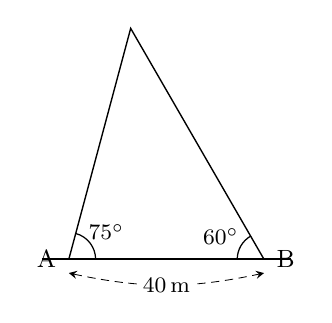
\begin{tikzpicture}[scale=0.62, line width=0.5pt, >=stealth]
  \coordinate (A) at (0,0);
  \coordinate (B) at (4,0);
  \coordinate (P) at (1.268,4.732);
  \draw[line width=0.7pt] (-0.55,0) -- (4.55,0);
  \draw (A) -- (P) -- (B);
  \draw[line width=0.45pt] ([shift=(0:0.55)]A) arc (0:75:0.55);
  \draw[line width=0.45pt] ([shift=(180:0.55)]B) arc (180:120:0.55);
  \node[font=\footnotesize] at ([shift=(36:0.95)]A) {$75^\circ$};
  \node[font=\footnotesize] at ([shift=(152:1.0)]B) {$60^\circ$};
  \node[left=1pt, font=\small] at (A) {$\pt{A}$};
  \node[right=1pt, font=\small] at (B) {$\pt{B}$};
  \draw[densely dashed, line width=0.3pt, <->] (0,-0.28)
    to[bend right=12] node[midway, fill=white, inner sep=1pt, font=\footnotesize] {$40\,\mathrm{m}$} (4,-0.28);
\end{tikzpicture}
}\end{minipage}\par
\begin{choicesii}{\rule[-3ex]{0pt}{8ex}$20\sqrt{2}\mkern3mu \mathrm{m}$}{\rule[-3ex]{0pt}{8ex}$30\mkern3mu \mathrm{m}$}{\rule[-3ex]{0pt}{8ex}$20\sqrt{3}\mkern3mu \mathrm{m}$}{\rule[-3ex]{0pt}{8ex}$36\mkern3mu \mathrm{m}$}{\rule[-3ex]{0pt}{8ex}$20\sqrt{6}\mkern3mu \mathrm{m}$}\end{choicesii}
}\vspace{8mm}
\vspace{3mm}\setcounter{dmproblemcount}{19}\dmpnum{143-20}{% id: 143-20
% book: 베이직쎈 대수 · 08 삼각함수의 활용
% section: 유형 084 사인법칙과 코사인법칙의 실생활에의 활용
% figure: tikz:fig-143-20
% answer: 
% answer_source: 
% variant_level: 0 (원본 전사)
% 이 파일은 build.mjs 가 items.json 에서 만든다. 고칠 때는 items.json 을 고친다.
\smash{\raisebox{4.5mm}{\dmkichul{베이직쎈 대수 143쪽 20번}}}
\noindent\begin{minipage}[t]{0.58\linewidth}\vspace{0pt}\raggedright 오른쪽 그림과 같이 $50\sqrt{3}\mkern3mu \mathrm{m}$ 떨어진 두 지점~$\pt{A}$, $\pt{B}$에서 분수대가 있는 $\pt{C}$ 지점을 바라본 각의 크기를 재었더니 $\angle\pt{A}=75^\circ$, $\angle\pt{B}=45^\circ$이었다. 세 지점~$\pt{A}$, $\pt{B}$, $\pt{C}$를 연결하는 원 모양의 잔디밭을 만들려고 할 때, 잔디밭의 넓이를 구하시오.\end{minipage}\hfill\begin{minipage}[t]{0.4\linewidth}\vspace{0pt}\centering \resizebox{\ifdim\width>\linewidth\linewidth\else\width\fi}{!}{% 143-20(143쪽) — 세 지점 A, B, C 를 지나는 원 모양의 잔디밭과 삼각형 ABC · ∠A=75°, ∠B=45°, AB=50√3 m.
% 스캔 삽화(연두색 잔디밭 바탕·분수대 그림)는 화질이 낮아 TikZ 로 다시 그렸다 — 원(잔디밭)은 문제의 조건이라 남기고 분수대 그림은 뺐다.
% 라벨은 원문에 있는 A·B·C·75°·45°·50√3 m 만 두고 잔디밭의 넓이(답)는 적지 않는다.
\begin{tikzpicture}[scale=1.15, line width=0.5pt, >=stealth]
  \coordinate (A) at (100:1);
  \coordinate (B) at (220:1);
  \coordinate (C) at (10:1);
  \fill[yellow!35] (0,0) circle (1);
  \draw[line width=0.4pt, yellow!60!black] (0,0) circle (1);
  \draw (A) -- (B) -- (C) -- cycle;
  \draw[line width=0.4pt] ([shift=(250:0.24)]A) arc (250:325:0.24);
  \draw[line width=0.4pt] ([shift=(25:0.26)]B) arc (25:70:0.26);
  \node[font=\footnotesize] at ([shift=(288:0.4)]A) {$75^\circ$};
  \node[font=\footnotesize] at ([shift=(48:0.44)]B) {$45^\circ$};
  \node[above=0pt, font=\small] at (A) {$\pt{A}$};
  \node[below=0pt, font=\small] at (B) {$\pt{B}$};
  \node[below right=-3pt and -2pt, font=\small] at (C) {$\pt{C}$};
  \draw[densely dashed, line width=0.3pt, <->] (-0.400,1.077) -- (-0.992,-0.550);
  \node[left=2pt, font=\footnotesize] at (-0.700,0.225) {$50\sqrt{3}\,\mathrm{m}$};
\end{tikzpicture}
}\end{minipage}\par
}\vspace{8mm}
\setcounter{dmproblemcount}{20}\dmpnum{143-21}{% id: 143-21
% book: 베이직쎈 대수 · 08 삼각함수의 활용
% section: 유형 084 사인법칙과 코사인법칙의 실생활에의 활용
% figure: tikz:fig-143-21
% answer: 
% answer_source: 
% variant_level: 0 (원본 전사)
% 이 파일은 build.mjs 가 items.json 에서 만든다. 고칠 때는 items.json 을 고친다.
\smash{\raisebox{1.5mm}{\dmkichul{베이직쎈 대수 143쪽 21번}}}
\noindent\begin{minipage}[t]{0.58\linewidth}\vspace{0pt}\raggedright 오른쪽 그림과 같이 호수의 가장자리에 있는 두 나무~$\pt{A}$, $\pt{B}$ 사이의 거리를 구하기 위하여 $\pt{C}$ 지점에서 측량하였더니 $\seg{AC}=\seg{BC}=200\mkern3mu \mathrm{m}$, $\angle\pt{C}=120^\circ$이었다. 이때 두 나무~$\pt{A}$, $\pt{B}$ 사이의 거리는?\end{minipage}\hfill\begin{minipage}[t]{0.4\linewidth}\vspace{0pt}\centering \resizebox{\ifdim\width>\linewidth\linewidth\else\width\fi}{!}{% 143-21(143쪽) — 호수 가장자리의 두 나무 A, B 와 측량 지점 C · AC=BC=200 m, ∠C=120°.
% 스캔 삽화(호수 물결·나무 그림)는 화질이 낮아 TikZ 로 다시 그렸다 — 호수는 A, B 를 잇는 선 위쪽의 연한 영역으로만 남겼다.
% 라벨은 원문에 있는 A·B·C·200 m·120° 만 두고 두 나무 사이의 거리(답)는 적지 않는다.
\begin{tikzpicture}[scale=0.78, line width=0.5pt]
  \coordinate (A) at (-2,0);
  \coordinate (B) at (2,0);
  \coordinate (C) at (0,-1.155);
  \fill[cyan!18] (A) .. controls (-1.9,1.45) and (1.9,1.45) .. (B) -- cycle;
  \draw[line width=0.4pt, cyan!55!black] (A) .. controls (-1.9,1.45) and (1.9,1.45) .. (B);
  \draw (A) -- (B) -- (C) -- cycle;
  \draw[line width=0.4pt] ([shift=(30:0.42)]C) arc (30:150:0.42);
  \node[font=\footnotesize] at ([shift=(90:0.66)]C) {$120^\circ$};
  \node[above left=-3pt and -2pt, font=\small] at (A) {$\pt{A}$};
  \node[above right=-3pt and -2pt, font=\small] at (B) {$\pt{B}$};
  \node[below=0pt, font=\small] at (C) {$\pt{C}$};
  \node[left=3pt, font=\footnotesize] at (-1,-0.578) {$200\,\mathrm{m}$};
  \node[right=3pt, font=\footnotesize] at (1,-0.578) {$200\,\mathrm{m}$};
\end{tikzpicture}
}\end{minipage}\par
\begin{choices32}{\rule[-3ex]{0pt}{8ex}$150\sqrt{2}\mkern3mu \mathrm{m}$}{\rule[-3ex]{0pt}{8ex}$260\mkern3mu \mathrm{m}$}{\rule[-3ex]{0pt}{8ex}$200\sqrt{2}\mkern3mu \mathrm{m}$}{\rule[-3ex]{0pt}{8ex}$300\mkern3mu \mathrm{m}$}{\rule[-3ex]{0pt}{8ex}$200\sqrt{3}\mkern3mu \mathrm{m}$}\end{choices32}
}\vspace{8mm}
\setcounter{dmproblemcount}{21}\dmpnum{143-22}{% id: 143-22
% book: 베이직쎈 대수 · 08 삼각함수의 활용
% section: 유형 084 사인법칙과 코사인법칙의 실생활에의 활용
% figure: tikz:fig-143-22
% answer: 
% answer_source: 
% variant_level: 0 (원본 전사)
% 이 파일은 build.mjs 가 items.json 에서 만든다. 고칠 때는 items.json 을 고친다.
\smash{\raisebox{1.5mm}{\dmkichul{베이직쎈 대수 143쪽 22번}}}
\noindent\begin{minipage}[t]{0.58\linewidth}\vspace{0pt}\raggedright 항구~$\pt{A}$를 출발한 배가 동쪽으로 $3\mkern3mu \mathrm{km}$를 항해한 후 오른쪽 그림과 같이 북동쪽으로 각 $\theta$만큼 방향을 바꾸어 $6\mkern3mu \mathrm{km}$를 가서 항구~$\pt{B}$에 도착하였다. 두 항구~$\pt{A}$, $\pt{B}$ 사이의 거리가 $3\sqrt{7}\mkern3mu \mathrm{km}$일 때, $\theta$의 값을 구하시오.\end{minipage}\hfill\begin{minipage}[t]{0.4\linewidth}\vspace{0pt}\centering \resizebox{\ifdim\width>\linewidth\linewidth\else\width\fi}{!}{% 143-22(143쪽) — 항구 A 에서 동쪽으로 3 km 간 지점 C 에서 각 θ 만큼 방향을 바꿔 6 km 를 가 항구 B 에 이르는 항로 · AB=3√7 km.
% 스캔 삽화(바다 바탕·등대·배 그림)는 화질이 낮아 TikZ 로 기하만 다시 그렸다.
% 라벨은 원문에 있는 A·B·C·3 km·6 km·3√7 km·θ 만 두고 θ 의 값(답)은 적지 않는다.
\begin{tikzpicture}[scale=0.52, line width=0.5pt]
  \coordinate (A) at (0,0);
  \coordinate (C) at (3,0);
  \coordinate (B) at (6,5.196);
  \draw[densely dotted, line width=0.3pt] (C) -- (5.4,0);
  \draw (A) -- (C) -- (B) -- cycle;
  \draw[line width=0.4pt] ([shift=(0:0.78)]C) arc (0:60:0.78);
  \node[font=\footnotesize] at ([shift=(30:1.15)]C) {$\theta$};
  \node[below left=-3pt and -3pt, font=\small] at (A) {$\pt{A}$};
  \node[below right=-3pt and -3pt, font=\small] at (C) {$\pt{C}$};
  \node[right=1pt, font=\small] at (B) {$\pt{B}$};
  \node[below=0pt, font=\footnotesize] at (1.5,0) {$3\,\mathrm{km}$};
  \node[right=2pt, font=\footnotesize] at (4.6,2.5) {$6\,\mathrm{km}$};
  \node[left=2pt, font=\footnotesize] at (3,2.598) {$3\sqrt{7}\,\mathrm{km}$};
\end{tikzpicture}
}\end{minipage}\par
}\vspace{8mm}
\dmsection{개념 51 삼각형의 넓이}
\dmpassage{다음 삼각형~$\pt{ABC}$의 넓이를 구하시오.}
\setcounter{dmproblemcount}{0}\dmpnum{144-01}{% id: 144-01
% book: 베이직쎈 대수 · 08 삼각함수의 활용
% section: 개념 51 삼각형의 넓이
% passage: 다음 삼각형~$\pt{ABC}$의 넓이를 구하시오.
% figure: tikz:fig-144-01
% answer: 
% answer_source: 
% variant_level: 0 (원본 전사)
% 이 파일은 build.mjs 가 items.json 에서 만든다. 고칠 때는 items.json 을 고친다.
\smash{\raisebox{1.5mm}{\dmkichul{베이직쎈 대수 144쪽 01번}}}

\par\smallskip\begin{center}\resizebox{\ifdim\width>\linewidth\linewidth\else\width\fi}{!}{% 144-01(144쪽) — 색칠한 삼각형 ABC(B 왼쪽 아래 · C 오른쪽 아래 · A 위) · AB=4, ∠B=30°, BC=6.
% 스캔 그림이라 화질이 낮아 TikZ 로 다시 그렸다. 라벨은 원문에 있는 A·B·C·4·30°·6 만 두고 넓이(답)는 적지 않는다.
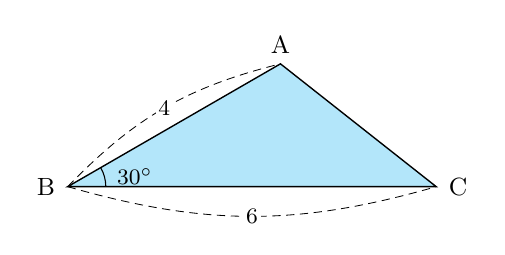
\begin{tikzpicture}[scale=0.78, line width=0.5pt]
  \coordinate (B) at (0,0);
  \coordinate (C) at (6,0);
  \coordinate (A) at (3.464,2);
  \fill[cyan!30] (A) -- (B) -- (C) -- cycle;
  \draw (A) -- (B) -- (C) -- cycle;
  \draw[line width=0.4pt] ([shift=(0:0.62)]B) arc (0:30:0.62);
  \node[right=1pt, font=\footnotesize] at ([shift=(15:0.62)]B) {$30^\circ$};
  \node[above=0pt, font=\small] at (A) {$\pt{A}$};
  \node[left=1pt, font=\small] at (B) {$\pt{B}$};
  \node[right=1pt, font=\small] at (C) {$\pt{C}$};
  \draw[densely dashed, line width=0.3pt] (B)
    to[bend left=16] node[midway, fill=white, inner sep=1pt, font=\footnotesize] {$4$} (A);
  \draw[densely dashed, line width=0.3pt] (B)
    to[bend right=16] node[midway, fill=white, inner sep=1pt, font=\footnotesize] {$6$} (C);
\end{tikzpicture}
}\end{center}
\dmhint{$\triangle\pt{ABC}=\dfrac{1}{2}\times\seg{AB}\times\seg{BC}\times\sin B$\\ \hspace*{1.5em}$=\dfrac{1}{2}\times\blank\times 6\times\sin\blank^\circ$\\ \hspace*{1.5em}$=\blank$}
}\vspace{8mm}
\setcounter{dmproblemcount}{1}\dmpnum{144-02}{% id: 144-02
% book: 베이직쎈 대수 · 08 삼각함수의 활용
% section: 개념 51 삼각형의 넓이
% passage: 다음 삼각형~$\pt{ABC}$의 넓이를 구하시오.
% figure: tikz:fig-144-02
% answer: 
% answer_source: 
% variant_level: 0 (원본 전사)
% 이 파일은 build.mjs 가 items.json 에서 만든다. 고칠 때는 items.json 을 고친다.
\smash{\raisebox{1.5mm}{\dmkichul{베이직쎈 대수 144쪽 02번}}}

\par\smallskip\begin{center}\resizebox{\ifdim\width>\linewidth\linewidth\else\width\fi}{!}{% 144-02(144쪽) — 색칠한 삼각형 ABC(B 왼쪽 아래 · C 그 오른쪽 · A 오른쪽 위) · BC=5, ∠C=120°, CA=8.
% 스캔 그림이라 화질이 낮아 TikZ 로 다시 그렸다. 라벨은 원문에 있는 A·B·C·5·120°·8 만 두고 넓이(답)는 적지 않는다.
\begin{tikzpicture}[scale=0.5, line width=0.5pt]
  \coordinate (B) at (0,0);
  \coordinate (C) at (5,0);
  \coordinate (A) at (9,6.928);
  \fill[orange!30] (A) -- (B) -- (C) -- cycle;
  \draw (A) -- (B) -- (C) -- cycle;
  \draw[line width=0.4pt] ([shift=(180:0.95)]C) arc (180:60:0.95);
  \node[font=\footnotesize] at ([shift=(122:1.45)]C) {$120^\circ$};
  \node[above=0pt, font=\small] at (A) {$\pt{A}$};
  \node[left=1pt, font=\small] at (B) {$\pt{B}$};
  \node[below right=-3pt and -3pt, font=\small] at (C) {$\pt{C}$};
  \draw[densely dashed, line width=0.3pt] (B)
    to[bend right=16] node[midway, fill=white, inner sep=1pt, font=\footnotesize] {$5$} (C);
  \draw[densely dashed, line width=0.3pt] (C)
    to[bend right=14] node[midway, fill=white, inner sep=1pt, font=\footnotesize] {$8$} (A);
\end{tikzpicture}
}\end{center}
}\vspace{8mm}
\setcounter{dmproblemcount}{2}\dmpnum{144-03}{% id: 144-03
% book: 베이직쎈 대수 · 08 삼각함수의 활용
% section: 개념 51 삼각형의 넓이
% passage: 다음 삼각형~$\pt{ABC}$의 넓이를 구하시오.
% figure: none
% answer: 
% answer_source: 
% variant_level: 0 (원본 전사)
% 이 파일은 build.mjs 가 items.json 에서 만든다. 고칠 때는 items.json 을 고친다.
\smash{\raisebox{1.5mm}{\dmkichul{베이직쎈 대수 144쪽 03번}}}
$a=4$, $b=5$, $C=60^\circ$
}\vspace{8mm}
\setcounter{dmproblemcount}{3}\dmpnum{144-04}{% id: 144-04
% book: 베이직쎈 대수 · 08 삼각함수의 활용
% section: 개념 51 삼각형의 넓이
% passage: 다음 삼각형~$\pt{ABC}$의 넓이를 구하시오.
% figure: none
% answer: 
% answer_source: 
% variant_level: 0 (원본 전사)
% 이 파일은 build.mjs 가 items.json 에서 만든다. 고칠 때는 items.json 을 고친다.
\smash{\raisebox{1.5mm}{\dmkichul{베이직쎈 대수 144쪽 04번}}}
$b=7$, $c=8$, $A=45^\circ$
}\vspace{8mm}
\vspace{3mm}\setcounter{dmproblemcount}{4}\dmpnum{144-05}{% id: 144-05
% book: 베이직쎈 대수 · 08 삼각함수의 활용
% section: 개념 51 삼각형의 넓이
% passage: 다음 삼각형~$\pt{ABC}$의 넓이를 구하시오.
% figure: none
% answer: 
% answer_source: 
% variant_level: 0 (원본 전사)
% 이 파일은 build.mjs 가 items.json 에서 만든다. 고칠 때는 items.json 을 고친다.
\smash{\raisebox{4.5mm}{\dmkichul{베이직쎈 대수 144쪽 05번}}}
$a=6$, $c=4\sqrt{2}$, $B=135^\circ$
}\vspace{8mm}
\dmpassage{다음 삼각형의 넓이를 구하시오.}
\vspace{3mm}\setcounter{dmproblemcount}{5}\dmpnum{144-06}{% id: 144-06
% book: 베이직쎈 대수 · 08 삼각함수의 활용
% section: 개념 51 삼각형의 넓이
% passage: 다음 삼각형의 넓이를 구하시오.
% figure: none
% answer: 
% answer_source: 
% variant_level: 0 (원본 전사)
% 이 파일은 build.mjs 가 items.json 에서 만든다. 고칠 때는 items.json 을 고친다.
\smash{\raisebox{4.5mm}{\dmkichul{베이직쎈 대수 144쪽 06번}}}
세 변의 길이가 각각 $6$, $2\sqrt{5}$, $2\sqrt{2}$이고 외접원의 반지름의 길이가 $\sqrt{10}$인 삼각형
}\vspace{8mm}
\vspace{3mm}\setcounter{dmproblemcount}{6}\dmpnum{144-07}{% id: 144-07
% book: 베이직쎈 대수 · 08 삼각함수의 활용
% section: 개념 51 삼각형의 넓이
% passage: 다음 삼각형의 넓이를 구하시오.
% figure: none
% answer: 
% answer_source: 
% variant_level: 0 (원본 전사)
% 이 파일은 build.mjs 가 items.json 에서 만든다. 고칠 때는 items.json 을 고친다.
\smash{\raisebox{4.5mm}{\dmkichul{베이직쎈 대수 144쪽 07번}}}
세 변의 길이가 각각 $7$, $8$, $9$이고 외접원의 반지름의 길이가 $\dfrac{21\sqrt{5}}{10}$인 삼각형
}\vspace{8mm}
\vspace{3mm}\setcounter{dmproblemcount}{7}\dmpnum{144-08}{% id: 144-08
% book: 베이직쎈 대수 · 08 삼각함수의 활용
% section: 개념 51 삼각형의 넓이
% passage: 다음 삼각형의 넓이를 구하시오.
% figure: none
% answer: 
% answer_source: 
% variant_level: 0 (원본 전사)
% 이 파일은 build.mjs 가 items.json 에서 만든다. 고칠 때는 items.json 을 고친다.
\smash{\raisebox{4.5mm}{\dmkichul{베이직쎈 대수 144쪽 08번}}}
세 내각의 크기가 각각 $\dfrac{\pi}{6}$, $\dfrac{\pi}{2}$, $\dfrac{\pi}{3}$이고 외접원의 반지름의 길이가 $5$인 삼각형
}\vspace{8mm}
\vspace{3mm}\setcounter{dmproblemcount}{8}\dmpnum{144-09}{% id: 144-09
% book: 베이직쎈 대수 · 08 삼각함수의 활용
% section: 개념 51 삼각형의 넓이
% passage: 다음 삼각형의 넓이를 구하시오.
% figure: none
% answer: 
% answer_source: 
% variant_level: 0 (원본 전사)
% 이 파일은 build.mjs 가 items.json 에서 만든다. 고칠 때는 items.json 을 고친다.
\smash{\raisebox{4.5mm}{\dmkichul{베이직쎈 대수 144쪽 09번}}}
세 내각의 크기가 각각 $\dfrac{\pi}{4}$, $\dfrac{\pi}{4}$, $\dfrac{\pi}{2}$이고 외접원의 반지름의 길이가 $4\sqrt{2}$인 삼각형
}\vspace{8mm}
\dmsection{개념 52 사각형의 넓이}
\dmpassage{다음 평행사변형~$\pt{ABCD}$의 넓이를 구하시오.}
\setcounter{dmproblemcount}{9}\dmpnum{145-10}{% id: 145-10
% book: 베이직쎈 대수 · 08 삼각함수의 활용
% section: 개념 52 사각형의 넓이
% passage: 다음 평행사변형~$\pt{ABCD}$의 넓이를 구하시오.
% figure: tikz:fig-145-10
% answer: 
% answer_source: 
% variant_level: 0 (원본 전사)
% 이 파일은 build.mjs 가 items.json 에서 만든다. 고칠 때는 items.json 을 고친다.
\smash{\raisebox{1.5mm}{\dmkichul{베이직쎈 대수 145쪽 10번}}}

\par\smallskip\begin{center}\resizebox{\ifdim\width>\linewidth\linewidth\else\width\fi}{!}{% 145-10(145쪽) — 평행사변형 ABCD · AB=5, BC=6, ∠B=60°. 스캔 화질이 낮아 TikZ 로 다시 그림.
% 원문에 있는 5 · 6 · 60° 만 적는다(넓이는 답이므로 그림에 적지 않는다).
\begin{tikzpicture}[line width=0.6pt, x=0.52cm, y=0.52cm]
  \coordinate (A) at (2.5,4.33);
  \coordinate (B) at (0,0);
  \coordinate (C) at (6,0);
  \coordinate (D) at (8.5,4.33);
  \draw (A) -- (B) -- (C) -- (D) -- cycle;
  \draw[densely dotted, line width=0.35pt] (2.3,4.4) to[bend right=18] node[midway, left=-2pt, font=\footnotesize] {$5$} (-0.25,0.05);
  \draw[densely dotted, line width=0.35pt] (0.05,-0.3) to[bend right=16] node[midway, below=-2.5pt, font=\footnotesize] {$6$} (5.95,-0.3);
  \draw[line width=0.4pt] ([shift=(0:0.9)]B) arc (0:60:0.9);
  \node[font=\footnotesize] at ([shift=(28:1.85)]B) {$60^\circ$};
  \node[above left=-3pt and -3.5pt, font=\footnotesize] at (A) {$\pt{A}$};
  \node[above right=-3pt and -3.5pt, font=\footnotesize] at (D) {$\pt{D}$};
  \node[below left=-2.5pt and -2.5pt, font=\footnotesize] at (B) {$\pt{B}$};
  \node[below right=-2.5pt and -2.5pt, font=\footnotesize] at (C) {$\pt{C}$};
\end{tikzpicture}
}\end{center}
\dmhint{평행사변형의 넓이를 $S$라 하면\\ \hspace*{1.5em}$S=\seg{AB}\times\seg{BC}\times\sin B$\\ \hspace*{2.6em}$=5\times\blank\times\sin\blank^\circ$\\ \hspace*{2.6em}$=\blank$}
}\vspace{8mm}
\setcounter{dmproblemcount}{10}\dmpnum{145-11}{% id: 145-11
% book: 베이직쎈 대수 · 08 삼각함수의 활용
% section: 개념 52 사각형의 넓이
% passage: 다음 평행사변형~$\pt{ABCD}$의 넓이를 구하시오.
% figure: tikz:fig-145-11
% answer: 
% answer_source: 
% variant_level: 0 (원본 전사)
% 이 파일은 build.mjs 가 items.json 에서 만든다. 고칠 때는 items.json 을 고친다.
\smash{\raisebox{1.5mm}{\dmkichul{베이직쎈 대수 145쪽 11번}}}

\par\smallskip\begin{center}\resizebox{\ifdim\width>\linewidth\linewidth\else\width\fi}{!}{% 145-11(145쪽) — 평행사변형 ABCD · DC=3, BC=4, ∠C=30°. 스캔 화질이 낮아 TikZ 로 다시 그림.
% 원문에 있는 3 · 4 · 30° 만 적는다.
\begin{tikzpicture}[line width=0.6pt, x=0.66cm, y=0.66cm]
  \coordinate (A) at (0,1.5);
  \coordinate (B) at (2.598,0);
  \coordinate (C) at (6.598,0);
  \coordinate (D) at (4,1.5);
  \draw (A) -- (B) -- (C) -- (D) -- cycle;
  \draw[densely dotted, line width=0.35pt] (4.15,1.62) to[bend left=20] node[midway, right=-2.5pt, font=\footnotesize] {$3$} (6.75,0.08);
  \draw[densely dotted, line width=0.35pt] (2.65,-0.3) to[bend right=16] node[midway, below=-2.5pt, font=\footnotesize] {$4$} (6.55,-0.3);
  \draw[line width=0.4pt] ([shift=(150:0.85)]C) arc (150:180:0.85);
  \node[font=\footnotesize] at ([shift=(163:1.5)]C) {$30^\circ$};
  \node[above left=-3pt and -3.5pt, font=\footnotesize] at (A) {$\pt{A}$};
  \node[above=-2.5pt, font=\footnotesize] at (D) {$\pt{D}$};
  \node[below left=-2.5pt and -2.5pt, font=\footnotesize] at (B) {$\pt{B}$};
  \node[right=-2pt, font=\footnotesize] at (C) {$\pt{C}$};
\end{tikzpicture}
}\end{center}
}\vspace{8mm}
\setcounter{dmproblemcount}{11}\dmpnum{145-12}{% id: 145-12
% book: 베이직쎈 대수 · 08 삼각함수의 활용
% section: 개념 52 사각형의 넓이
% passage: 다음 평행사변형~$\pt{ABCD}$의 넓이를 구하시오.
% figure: tikz:fig-145-12
% answer: 
% answer_source: 
% variant_level: 0 (원본 전사)
% 이 파일은 build.mjs 가 items.json 에서 만든다. 고칠 때는 items.json 을 고친다.
\smash{\raisebox{1.5mm}{\dmkichul{베이직쎈 대수 145쪽 12번}}}

\par\smallskip\begin{center}\resizebox{\ifdim\width>\linewidth\linewidth\else\width\fi}{!}{% 145-12(145쪽) — 평행사변형 ABCD · AB=5, BC=4√2, ∠A=135°. 스캔 화질이 낮아 TikZ 로 다시 그림.
% 원문에 있는 5 · 4√2 · 135° 만 적는다.
\begin{tikzpicture}[line width=0.6pt, x=0.48cm, y=0.48cm]
  \coordinate (A) at (3.536,3.536);
  \coordinate (B) at (0,0);
  \coordinate (C) at (5.657,0);
  \coordinate (D) at (9.193,3.536);
  \draw (A) -- (B) -- (C) -- (D) -- cycle;
  \draw[densely dotted, line width=0.35pt] (3.35,3.62) to[bend right=18] node[midway, left=-2pt, font=\footnotesize] {$5$} (-0.3,0.06);
  \draw[densely dotted, line width=0.35pt] (0.05,-0.35) to[bend right=16] node[midway, below=-2.5pt, font=\footnotesize] {$4\sqrt{2}$} (5.6,-0.35);
  \draw[line width=0.4pt] ([shift=(225:1.0)]A) arc (225:360:1.0);
  \node[font=\footnotesize] at ([shift=(295:1.85)]A) {$135^\circ$};
  \node[above=-2.5pt, font=\footnotesize] at (A) {$\pt{A}$};
  \node[above right=-3pt and -3.5pt, font=\footnotesize] at (D) {$\pt{D}$};
  \node[below left=-2.5pt and -2.5pt, font=\footnotesize] at (B) {$\pt{B}$};
  \node[below right=-2.5pt and -2.5pt, font=\footnotesize] at (C) {$\pt{C}$};
\end{tikzpicture}
}\end{center}
}\vspace{8mm}
\setcounter{dmproblemcount}{12}\dmpnum{145-13}{% id: 145-13
% book: 베이직쎈 대수 · 08 삼각함수의 활용
% section: 개념 52 사각형의 넓이
% passage: 다음 평행사변형~$\pt{ABCD}$의 넓이를 구하시오.
% figure: tikz:fig-145-13
% answer: 
% answer_source: 
% variant_level: 0 (원본 전사)
% 이 파일은 build.mjs 가 items.json 에서 만든다. 고칠 때는 items.json 을 고친다.
\smash{\raisebox{1.5mm}{\dmkichul{베이직쎈 대수 145쪽 13번}}}

\par\smallskip\begin{center}\resizebox{\ifdim\width>\linewidth\linewidth\else\width\fi}{!}{% 145-13(145쪽) — 평행사변형 ABCD · AB=6, BC=8, ∠D=150°. 스캔 화질이 낮아 TikZ 로 다시 그림.
% 원문에 있는 6 · 8 · 150° 만 적는다.
\begin{tikzpicture}[line width=0.6pt, x=0.33cm, y=0.33cm]
  \coordinate (A) at (0,3);
  \coordinate (B) at (5.196,0);
  \coordinate (C) at (13.196,0);
  \coordinate (D) at (8,3);
  \draw (A) -- (B) -- (C) -- (D) -- cycle;
  \draw[densely dotted, line width=0.35pt] (-0.35,2.85) to[bend right=18] node[midway, below left=-3.5pt and -3pt, font=\footnotesize] {$6$} (5.0,-0.35);
  \draw[densely dotted, line width=0.35pt] (5.3,-0.55) to[bend right=14] node[midway, below=-2.5pt, font=\footnotesize] {$8$} (13.1,-0.55);
  \draw[line width=0.4pt] ([shift=(180:1.2)]D) arc (180:330:1.2);
  \node[font=\footnotesize] at ([shift=(257:2.1)]D) {$150^\circ$};
  \node[above left=-3pt and -3.5pt, font=\footnotesize] at (A) {$\pt{A}$};
  \node[above=-2.5pt, font=\footnotesize] at (D) {$\pt{D}$};
  \node[below left=-2.5pt and -2.5pt, font=\footnotesize] at (B) {$\pt{B}$};
  \node[below right=-2.5pt and -2.5pt, font=\footnotesize] at (C) {$\pt{C}$};
\end{tikzpicture}
}\end{center}
}\vspace{8mm}
\dmpassage{다음 사각형~$\pt{ABCD}$의 넓이를 구하시오.}
\setcounter{dmproblemcount}{13}\dmpnum{145-14}{% id: 145-14
% book: 베이직쎈 대수 · 08 삼각함수의 활용
% section: 개념 52 사각형의 넓이
% passage: 다음 사각형~$\pt{ABCD}$의 넓이를 구하시오.
% figure: tikz:fig-145-14
% answer: 
% answer_source: 
% variant_level: 0 (원본 전사)
% 이 파일은 build.mjs 가 items.json 에서 만든다. 고칠 때는 items.json 을 고친다.
\smash{\raisebox{1.5mm}{\dmkichul{베이직쎈 대수 145쪽 14번}}}

\par\smallskip\begin{center}\resizebox{\ifdim\width>\linewidth\linewidth\else\width\fi}{!}{% 145-14(145쪽) — 사각형 ABCD · 두 대각선 AC=10, BD=8 이 이루는 각 120°. 스캔 화질이 낮아 TikZ 로 다시 그림.
% 원문에 있는 8 · 10 · 120° 만 적는다(넓이는 답이므로 그림에 적지 않는다).
\begin{tikzpicture}[line width=0.6pt, x=0.50cm, y=0.50cm]
  \coordinate (A) at (-3.897,2.25);
  \coordinate (B) at (-3.118,-1.8);
  \coordinate (C) at (4.763,-2.75);
  \coordinate (D) at (3.811,2.2);
  \coordinate (P) at (0,0);
  \draw (A) -- (B) -- (C) -- (D) -- cycle;
  \draw (A) -- (C);
  \draw (B) -- (D);
  \draw[densely dotted, line width=0.35pt] (-3.25,-1.62) to[bend left=15] node[pos=0.3, above left=-4pt and -4pt, font=\footnotesize] {$8$} (3.68,2.38);
  \draw[densely dotted, line width=0.35pt] (-3.77,2.42) to[bend left=15] node[pos=0.72, above right=-4pt and -4pt, font=\footnotesize] {$10$} (4.9,-2.6);
  \draw[line width=0.4pt] ([shift=(210:0.62)]P) arc (210:330:0.62);
  \node[font=\footnotesize] at ([shift=(270:1.3)]P) {$120^\circ$};
  \node[above left=-3pt and -3.5pt, font=\footnotesize] at (A) {$\pt{A}$};
  \node[above right=-3pt and -3.5pt, font=\footnotesize] at (D) {$\pt{D}$};
  \node[below left=-2.5pt and -2.5pt, font=\footnotesize] at (B) {$\pt{B}$};
  \node[below right=-2.5pt and -2.5pt, font=\footnotesize] at (C) {$\pt{C}$};
\end{tikzpicture}
}\end{center}
\dmhint{사각형의 넓이를 $S$라 하면\\ \hspace*{1.5em}$S=\dfrac{1}{2}\times\seg{AC}\times\seg{BD}\times\sin 120^\circ$\\ \hspace*{2.6em}$=\dfrac{1}{2}\times\blank\times 8\times\blank$\\ \hspace*{2.6em}$=\blank$}
}\vspace{8mm}
\setcounter{dmproblemcount}{14}\dmpnum{145-15}{% id: 145-15
% book: 베이직쎈 대수 · 08 삼각함수의 활용
% section: 개념 52 사각형의 넓이
% passage: 다음 사각형~$\pt{ABCD}$의 넓이를 구하시오.
% figure: tikz:fig-145-15
% answer: 
% answer_source: 
% variant_level: 0 (원본 전사)
% 이 파일은 build.mjs 가 items.json 에서 만든다. 고칠 때는 items.json 을 고친다.
\smash{\raisebox{1.5mm}{\dmkichul{베이직쎈 대수 145쪽 15번}}}

\par\smallskip\begin{center}\resizebox{\ifdim\width>\linewidth\linewidth\else\width\fi}{!}{% 145-15(145쪽) — 사각형 ABCD · 두 대각선 AC=2√5, BD=4 가 이루는 각 135°. 스캔 화질이 낮아 TikZ 로 다시 그림.
% 원문에 있는 2√5 · 4 · 135° 만 적는다.
\begin{tikzpicture}[line width=0.6pt, x=0.50cm, y=0.50cm]
  \coordinate (A) at (-3.678,1.524);
  \coordinate (B) at (-4.176,-1.730);
  \coordinate (C) at (4.582,-1.898);
  \coordinate (D) at (3.344,1.386);
  \coordinate (P) at (0,0);
  \draw (A) -- (B) -- (C) -- (D) -- cycle;
  \draw (A) -- (C);
  \draw (B) -- (D);
  \draw[densely dotted, line width=0.35pt] (-3.6,1.36) to[bend right=13] node[pos=0.28, below left=-4pt and -4.5pt, font=\footnotesize] {$2\sqrt{5}$} (4.5,-2.06);
  \draw[densely dotted, line width=0.35pt] (-4.1,-1.89) to[bend right=13] node[pos=0.78, below right=-4pt and -4pt, font=\footnotesize] {$4$} (3.42,1.22);
  \draw[line width=0.4pt] ([shift=(22.5:0.55)]P) arc (22.5:157.5:0.55);
  \node[font=\footnotesize] at ([shift=(90:1.02)]P) {$135^\circ$};
  \node[above left=-3pt and -3.5pt, font=\footnotesize] at (A) {$\pt{A}$};
  \node[above right=-3pt and -3.5pt, font=\footnotesize] at (D) {$\pt{D}$};
  \node[below left=-2.5pt and -2.5pt, font=\footnotesize] at (B) {$\pt{B}$};
  \node[below right=-2.5pt and -2.5pt, font=\footnotesize] at (C) {$\pt{C}$};
\end{tikzpicture}
}\end{center}
}\vspace{8mm}
\setcounter{dmproblemcount}{15}\dmpnum{145-16}{% id: 145-16
% book: 베이직쎈 대수 · 08 삼각함수의 활용
% section: 개념 52 사각형의 넓이
% passage: 다음 사각형~$\pt{ABCD}$의 넓이를 구하시오.
% figure: tikz:fig-145-16
% answer: 
% answer_source: 
% variant_level: 0 (원본 전사)
% 이 파일은 build.mjs 가 items.json 에서 만든다. 고칠 때는 items.json 을 고친다.
\smash{\raisebox{1.5mm}{\dmkichul{베이직쎈 대수 145쪽 16번}}}

\par\smallskip\begin{center}\resizebox{\ifdim\width>\linewidth\linewidth\else\width\fi}{!}{% 145-16(145쪽) — 사각형 ABCD · 두 대각선 AC=4√3, BD=5 가 이루는 각 60°. 스캔 화질이 낮아 TikZ 로 다시 그림.
% 원문에 있는 5 · 4√3 · 60° 만 적는다.
\begin{tikzpicture}[line width=0.6pt, x=0.50cm, y=0.50cm]
  \coordinate (A) at (-3.227,1.863);
  \coordinate (B) at (-4.143,-2.392);
  \coordinate (C) at (4.573,-2.640);
  \coordinate (D) at (1.599,0.923);
  \coordinate (P) at (0,0);
  \draw (A) -- (B) -- (C) -- (D) -- cycle;
  \draw (A) -- (C);
  \draw (B) -- (D);
  \draw[densely dotted, line width=0.35pt] (-4.28,-2.24) to[bend left=13] node[pos=0.32, above left=-4pt and -4pt, font=\footnotesize] {$5$} (1.5,1.08);
  \draw[densely dotted, line width=0.35pt] (-3.13,1.7) to[bend right=13] node[pos=0.48, below left=-4pt and -4.5pt, font=\footnotesize] {$4\sqrt{3}$} (4.49,-2.79);
  \draw[line width=0.4pt] ([shift=(-30:0.7)]P) arc (-30:30:0.7);
  \node[font=\footnotesize] at ([shift=(0:1.35)]P) {$60^\circ$};
  \node[above left=-3pt and -3.5pt, font=\footnotesize] at (A) {$\pt{A}$};
  \node[above right=-3pt and -3.5pt, font=\footnotesize] at (D) {$\pt{D}$};
  \node[below left=-2.5pt and -2.5pt, font=\footnotesize] at (B) {$\pt{B}$};
  \node[below right=-2.5pt and -2.5pt, font=\footnotesize] at (C) {$\pt{C}$};
\end{tikzpicture}
}\end{center}
}\vspace{8mm}
\setcounter{dmproblemcount}{16}\dmpnum{145-17}{% id: 145-17
% book: 베이직쎈 대수 · 08 삼각함수의 활용
% section: 개념 52 사각형의 넓이
% passage: 다음 사각형~$\pt{ABCD}$의 넓이를 구하시오.
% figure: tikz:fig-145-17
% answer: 
% answer_source: 
% variant_level: 0 (원본 전사)
% 이 파일은 build.mjs 가 items.json 에서 만든다. 고칠 때는 items.json 을 고친다.
\smash{\raisebox{1.5mm}{\dmkichul{베이직쎈 대수 145쪽 17번}}}

\par\smallskip\begin{center}\resizebox{\ifdim\width>\linewidth\linewidth\else\width\fi}{!}{% 145-17(145쪽) — 사각형 ABCD · 두 대각선 AC=9, BD=4 가 수직으로 만난다(직각 표시). 스캔 화질이 낮아 TikZ 로 다시 그림.
% 원문에 있는 4 · 9 · 직각 표시만 둔다(각의 크기 숫자는 원문에도 없다).
\begin{tikzpicture}[line width=0.6pt, x=0.50cm, y=0.50cm]
  \coordinate (A) at (-3.405,1.240);
  \coordinate (B) at (-0.709,-1.949);
  \coordinate (C) at (5.051,-1.839);
  \coordinate (D) at (0.688,1.890);
  \coordinate (P) at (0,0);
  \draw (A) -- (B) -- (C) -- (D) -- cycle;
  \draw (A) -- (C);
  \draw (B) -- (D);
  \draw[line width=0.35pt] (0.154,0.423) -- (-0.269,0.577) -- (-0.423,0.154);
  \draw[densely dotted, line width=0.35pt] (-0.56,-2.03) to[bend right=16] node[pos=0.72, right=-2.5pt, font=\footnotesize] {$4$} (0.83,1.82);
  \draw[densely dotted, line width=0.35pt] (-3.31,1.08) to[bend right=13] node[pos=0.58, below=-2.5pt, font=\footnotesize] {$9$} (5.0,-2.0);
  \node[left=-2pt, font=\footnotesize] at (A) {$\pt{A}$};
  \node[above right=-3pt and -3.5pt, font=\footnotesize] at (D) {$\pt{D}$};
  \node[below left=-2.5pt and -2.5pt, font=\footnotesize] at (B) {$\pt{B}$};
  \node[below right=-2.5pt and -2.5pt, font=\footnotesize] at (C) {$\pt{C}$};
\end{tikzpicture}
}\end{center}
}\vspace{8mm}
\dmsection{유형 085 삼각형의 넓이; $S=\dfrac{1}{2}ab\sin C$}
\setcounter{dmproblemcount}{0}\dmpnum{146-01}{% id: 146-01
% book: 베이직쎈 대수 · 08 삼각함수의 활용
% section: 유형 085 삼각형의 넓이; $S=\dfrac{1}{2}ab\sin C$
% figure: tikz:fig-146-01
% answer: 
% answer_source: 
% variant_level: 0 (원본 전사)
% 이 파일은 build.mjs 가 items.json 에서 만든다. 고칠 때는 items.json 을 고친다.
\smash{\raisebox{1.5mm}{\dmkichul{베이직쎈 대수 146쪽 01번}}}
\noindent\begin{minipage}[t]{0.58\linewidth}\vspace{0pt}\raggedright 오른쪽 그림과 같이 $\seg{AB}=8$, $\seg{AC}=7$이고, $B=60^\circ$, $C=75^\circ$인 삼각형~$\pt{ABC}$의 넓이를 구하시오.\end{minipage}\hfill\begin{minipage}[t]{0.4\linewidth}\vspace{0pt}\centering \resizebox{\ifdim\width>\linewidth\linewidth\else\width\fi}{!}{% 146-01(146쪽) — 삼각형 ABC · AB=8, AC=7, ∠B=60°, ∠C=75°. 스캔 화질이 낮아 TikZ 로 다시 그림.
% 원문에 있는 8 · 7 · 60° · 75° 만 적는다(넓이는 답이므로 그림에 적지 않는다).
\begin{tikzpicture}[line width=0.6pt, x=0.38cm, y=0.38cm]
  \coordinate (A) at (3.962,6.862);
  \coordinate (B) at (0,0);
  \coordinate (C) at (5.8,0);
  \draw (A) -- (B) -- (C) -- cycle;
  \draw[densely dotted, line width=0.35pt] (3.78,6.94) to[bend right=16] node[midway, left=-2.5pt, font=\footnotesize] {$8$} (-0.3,0.06);
  \draw[densely dotted, line width=0.35pt] (4.15,6.94) to[bend left=16] node[midway, right=-2.5pt, font=\footnotesize] {$7$} (6.1,0.06);
  \draw[line width=0.4pt] ([shift=(0:0.95)]B) arc (0:60:0.95);
  \node[font=\footnotesize] at ([shift=(32:1.75)]B) {$60^\circ$};
  \draw[line width=0.4pt] ([shift=(105:0.95)]C) arc (105:180:0.95);
  \node[font=\footnotesize] at ([shift=(144:1.8)]C) {$75^\circ$};
  \node[above=-2.5pt, font=\footnotesize] at (A) {$\pt{A}$};
  \node[below left=-2.5pt and -2.5pt, font=\footnotesize] at (B) {$\pt{B}$};
  \node[below right=-2.5pt and -2.5pt, font=\footnotesize] at (C) {$\pt{C}$};
\end{tikzpicture}
}\end{minipage}\par
}\vspace{8mm}
\vspace{3mm}\setcounter{dmproblemcount}{1}\dmpnum{146-02}{% id: 146-02
% book: 베이직쎈 대수 · 08 삼각함수의 활용
% section: 유형 085 삼각형의 넓이; $S=\dfrac{1}{2}ab\sin C$
% figure: none
% answer: 
% answer_source: 
% variant_level: 0 (원본 전사)
% 이 파일은 build.mjs 가 items.json 에서 만든다. 고칠 때는 items.json 을 고친다.
\smash{\raisebox{4.5mm}{\dmkichul{베이직쎈 대수 146쪽 02번}}}
삼각형~$\pt{ABC}$에서 $\seg{AB}=4\sqrt{2}$, $\seg{CA}=6$, $\cos A=\dfrac{1}{3}$일 때, 삼각형~$\pt{ABC}$의 넓이는?
\dmchoicesauto{}{$12$}{$14$}{$16$}{$18$}{$20$}
}\vspace{8mm}
\vspace{3mm}\setcounter{dmproblemcount}{2}\dmpnum{146-03}{% id: 146-03
% book: 베이직쎈 대수 · 08 삼각함수의 활용
% section: 유형 085 삼각형의 넓이; $S=\dfrac{1}{2}ab\sin C$
% figure: tikz:fig-146-03
% answer: 
% answer_source: 
% variant_level: 0 (원본 전사)
% 이 파일은 build.mjs 가 items.json 에서 만든다. 고칠 때는 items.json 을 고친다.
\smash{\raisebox{4.5mm}{\dmkichul{베이직쎈 대수 146쪽 03번}}}
\noindent\begin{minipage}[t]{0.58\linewidth}\vspace{0pt}\raggedright 오른쪽 그림과 같이 $\seg{AB}=\sqrt{13}$, $\seg{BC}=3$, $C=60^\circ$인 삼각형~$\pt{ABC}$의 넓이를 구하시오.\end{minipage}\hfill\begin{minipage}[t]{0.4\linewidth}\vspace{0pt}\centering \resizebox{\ifdim\width>\linewidth\linewidth\else\width\fi}{!}{% 146-03(146쪽) — 삼각형 ABC · AB=√13, BC=3, ∠C=60°. 스캔 화질이 낮아 TikZ 로 다시 그림.
% 원문에 있는 √13 · 3 · 60° 만 적는다(AC 의 길이·넓이는 적지 않는다).
\begin{tikzpicture}[line width=0.6pt, x=0.70cm, y=0.70cm]
  \coordinate (A) at (1,3.464);
  \coordinate (B) at (0,0);
  \coordinate (C) at (3,0);
  \draw (A) -- (B) -- (C) -- cycle;
  \draw[densely dotted, line width=0.35pt] (0.88,3.5) to[bend right=16] node[midway, left=-2.5pt, font=\footnotesize] {$\sqrt{13}$} (-0.16,0.04);
  \draw[densely dotted, line width=0.35pt] (0.04,-0.2) to[bend right=14] node[midway, below=-2.5pt, font=\footnotesize] {$3$} (2.96,-0.2);
  \draw[line width=0.4pt] ([shift=(120:0.55)]C) arc (120:180:0.55);
  \node[font=\footnotesize] at ([shift=(150:1.05)]C) {$60^\circ$};
  \node[above=-2.5pt, font=\footnotesize] at (A) {$\pt{A}$};
  \node[below left=-2.5pt and -2.5pt, font=\footnotesize] at (B) {$\pt{B}$};
  \node[below right=-2.5pt and -2.5pt, font=\footnotesize] at (C) {$\pt{C}$};
\end{tikzpicture}
}\end{minipage}\par
}\vspace{8mm}
\setcounter{dmproblemcount}{3}\dmpnum{146-04}{% id: 146-04
% book: 베이직쎈 대수 · 08 삼각함수의 활용
% section: 유형 085 삼각형의 넓이; $S=\dfrac{1}{2}ab\sin C$
% figure: none
% answer: 
% answer_source: 
% variant_level: 0 (원본 전사)
% 이 파일은 build.mjs 가 items.json 에서 만든다. 고칠 때는 items.json 을 고친다.
\smash{\raisebox{1.5mm}{\dmkichul{베이직쎈 대수 146쪽 04번}}}
삼각형~$\pt{ABC}$에서 $B=30^\circ$, $C=30^\circ$이고 외접원의 반지름의 길이가 4일 때, 다음을 구하시오.
\dmsubprob{1} $b$
\dmsubprob{2} $\triangle\pt{ABC}$의 넓이
}\vspace{8mm}
\setcounter{dmproblemcount}{4}\dmpnum{146-05}{% id: 146-05
% book: 베이직쎈 대수 · 08 삼각함수의 활용
% section: 유형 085 삼각형의 넓이; $S=\dfrac{1}{2}ab\sin C$
% figure: tikz:fig-146-05
% answer: 
% answer_source: 
% variant_level: 0 (원본 전사)
% 이 파일은 build.mjs 가 items.json 에서 만든다. 고칠 때는 items.json 을 고친다.
\smash{\raisebox{1.5mm}{\dmkichul{베이직쎈 대수 146쪽 05번}}}
\noindent\begin{minipage}[t]{0.58\linewidth}\vspace{0pt}\raggedright 오른쪽 그림과 같이 $A=60^\circ$, $\seg{AB}=8$, $\seg{AC}=6$인 삼각형~$\pt{ABC}$에서 $\angle\pt{A}$의 이등분선과 $\seg{BC}$의 교점을 $\pt{D}$라 할 때, $\seg{AD}$의 길이를 구하시오.\end{minipage}\hfill\begin{minipage}[t]{0.4\linewidth}\vspace{0pt}\centering \resizebox{\ifdim\width>\linewidth\linewidth\else\width\fi}{!}{% 146-05(146쪽) — 삼각형 ABC · AB=8, AC=6 · ∠A 의 이등분선이 BC 와 만나는 점 D. 스캔 화질이 낮아 TikZ 로 다시 그림.
% 원문처럼 8 · 6 과 ∠A 가 이등분됨을 나타내는 표시만 두고, AD 의 길이(답)는 적지 않는다.
\begin{tikzpicture}[line width=0.6pt, x=0.40cm, y=0.40cm]
  \coordinate (A) at (5.547,5.765);
  \coordinate (B) at (0,0);
  \coordinate (C) at (7.211,0);
  \coordinate (D) at (4.121,0);
  \draw (A) -- (B) -- (C) -- cycle;
  \draw (A) -- (D);
  \draw[densely dotted, line width=0.35pt] (5.42,5.9) to[bend right=14] node[midway, above left=-4pt and -4pt, font=\footnotesize] {$8$} (-0.18,0.12);
  \draw[densely dotted, line width=0.35pt] (5.72,5.88) to[bend left=14] node[midway, right=-2.5pt, font=\footnotesize] {$6$} (7.4,0.1);
  \draw[line width=0.35pt] ([shift=(226.1:1.05)]A) arc (226.1:256.1:1.05);
  \draw[line width=0.35pt] ([shift=(256.1:1.05)]A) arc (256.1:286.1:1.05);
  \draw[line width=0.35pt] ([shift=(241.1:0.88)]A) -- ([shift=(241.1:1.22)]A);
  \draw[line width=0.35pt] ([shift=(271.1:0.88)]A) -- ([shift=(271.1:1.22)]A);
  \node[above=-2.5pt, font=\footnotesize] at (A) {$\pt{A}$};
  \node[below left=-2.5pt and -2.5pt, font=\footnotesize] at (B) {$\pt{B}$};
  \node[below right=-2.5pt and -2.5pt, font=\footnotesize] at (C) {$\pt{C}$};
  \node[below=-2.5pt, font=\footnotesize] at (D) {$\pt{D}$};
\end{tikzpicture}
}\end{minipage}\par
}\vspace{8mm}
\vspace{3mm}\setcounter{dmproblemcount}{5}\dmpnum{146-06}{% id: 146-06
% book: 베이직쎈 대수 · 08 삼각함수의 활용
% section: 유형 085 삼각형의 넓이; $S=\dfrac{1}{2}ab\sin C$
% figure: tikz:fig-146-06
% answer: 
% answer_source: 
% variant_level: 0 (원본 전사)
% 이 파일은 build.mjs 가 items.json 에서 만든다. 고칠 때는 items.json 을 고친다.
\smash{\raisebox{4.5mm}{\dmkichul{베이직쎈 대수 146쪽 06번}}}
\noindent\begin{minipage}[t]{0.58\linewidth}\vspace{0pt}\raggedright 오른쪽 그림과 같이 $\seg{AB}=2$, $\seg{BC}=\sqrt{3}+1$, $\seg{CA}=\sqrt{2}$인 삼각형~$\pt{ABC}$의 넓이는?\end{minipage}\hfill\begin{minipage}[t]{0.4\linewidth}\vspace{0pt}\centering \resizebox{\ifdim\width>\linewidth\linewidth\else\width\fi}{!}{% 146-06(146쪽) — 삼각형 ABC · AB=2, BC=√3+1, CA=√2. 스캔 화질이 낮아 TikZ 로 다시 그림.
% 원문에 있는 세 변의 길이만 적는다(각의 크기·넓이는 적지 않는다).
\begin{tikzpicture}[line width=0.6pt, x=1.00cm, y=1.00cm]
  \coordinate (A) at (1.732,1);
  \coordinate (B) at (0,0);
  \coordinate (C) at (2.732,0);
  \draw (A) -- (B) -- (C) -- cycle;
  \draw[densely dotted, line width=0.35pt] (1.68,1.12) to[bend right=18] node[midway, above left=-4pt and -4pt, font=\footnotesize] {$2$} (-0.1,0.06);
  \draw[densely dotted, line width=0.35pt] (1.8,1.1) to[bend left=18] node[midway, above right=-4pt and -4pt, font=\footnotesize] {$\sqrt{2}$} (2.82,0.06);
  \draw[densely dotted, line width=0.35pt] (0.03,-0.14) to[bend right=12] node[midway, below=-2.5pt, font=\footnotesize] {$\sqrt{3}+1$} (2.7,-0.14);
  \node[above=-2.5pt, font=\footnotesize] at (A) {$\pt{A}$};
  \node[left=-2pt, font=\footnotesize] at (B) {$\pt{B}$};
  \node[right=-2pt, font=\footnotesize] at (C) {$\pt{C}$};
\end{tikzpicture}
}\end{minipage}\par
\begin{choices32}{\rule[-3ex]{0pt}{8ex}$\dfrac{\sqrt{2}}{2}$}{\rule[-3ex]{0pt}{8ex}$\dfrac{\sqrt{3}}{2}$}{\rule[-3ex]{0pt}{8ex}$\dfrac{\sqrt{3}+1}{2}$}{\rule[-3ex]{0pt}{8ex}$\sqrt{2}$}{\rule[-3ex]{0pt}{8ex}$\sqrt{3}$}\end{choices32}
}\vspace{8mm}
\dmsection{유형 086 외접원의 반지름의 길이와 삼각형의 넓이}
\vspace{3mm}\setcounter{dmproblemcount}{6}\dmpnum{147-07}{% id: 147-07
% book: 베이직쎈 대수 · 08 삼각함수의 활용
% section: 유형 086 외접원의 반지름의 길이와 삼각형의 넓이
% figure: none
% answer: 
% answer_source: 
% variant_level: 0 (원본 전사)
% 이 파일은 build.mjs 가 items.json 에서 만든다. 고칠 때는 items.json 을 고친다.
\smash{\raisebox{4.5mm}{\dmkichul{베이직쎈 대수 147쪽 07번}}}
세 변의 길이가 3, $\sqrt{5}$, $2\sqrt{2}$인 삼각형~$\pt{ABC}$의 넓이가 3일 때, 삼각형~$\pt{ABC}$의 외접원의 반지름의 길이를 구하시오.
}\vspace{8mm}
\vspace{3mm}\setcounter{dmproblemcount}{7}\dmpnum{147-08}{% id: 147-08
% book: 베이직쎈 대수 · 08 삼각함수의 활용
% section: 유형 086 외접원의 반지름의 길이와 삼각형의 넓이
% figure: none
% answer: 
% answer_source: 
% variant_level: 0 (원본 전사)
% 이 파일은 build.mjs 가 items.json 에서 만든다. 고칠 때는 items.json 을 고친다.
\smash{\raisebox{4.5mm}{\dmkichul{베이직쎈 대수 147쪽 08번}}}
세 변의 길이가 7, 8, 9인 삼각형~$\pt{ABC}$의 내접원의 반지름의 길이가 $\sqrt{5}$일 때, 삼각형~$\pt{ABC}$의 외접원의 반지름의 길이를 구하시오.
}\vspace{8mm}
\setcounter{dmproblemcount}{8}\dmpnum{147-09}{% id: 147-09
% book: 베이직쎈 대수 · 08 삼각함수의 활용
% section: 유형 086 외접원의 반지름의 길이와 삼각형의 넓이
% figure: tikz:fig-147-09
% answer: 
% answer_source: 
% variant_level: 0 (원본 전사)
% 이 파일은 build.mjs 가 items.json 에서 만든다. 고칠 때는 items.json 을 고친다.
\smash{\raisebox{1.5mm}{\dmkichul{베이직쎈 대수 147쪽 09번}}}
\noindent\begin{minipage}[t]{0.58\linewidth}\vspace{0pt}\raggedright 오른쪽 그림과 같은 이등변삼각형~$\pt{ABC}$에서 $B=C=30^\circ$이고, 삼각형~$\pt{ABC}$의 외접원의 반지름의 길이가 4일 때, 삼각형~$\pt{ABC}$의 넓이는?\end{minipage}\hfill\begin{minipage}[t]{0.4\linewidth}\vspace{0pt}\centering \resizebox{\ifdim\width>\linewidth\linewidth\else\width\fi}{!}{% 147-09(147쪽) — 반지름의 길이가 4인 원에 내접하는 이등변삼각형 ABC · ∠B=∠C=30°. 스캔 화질이 낮아 TikZ 로 다시 그림.
% 원문에 있는 반지름 4 와 두 30° 만 적는다(삼각형의 넓이는 답이므로 적지 않는다).
\begin{tikzpicture}[line width=0.6pt, x=0.32cm, y=0.32cm]
  \coordinate (O) at (0,0);
  \coordinate (A) at (2,3.464);
  \coordinate (B) at (-2,3.464);
  \coordinate (C) at (4,0);
  \draw[line width=0.55pt] (O) circle (4);
  \draw (A) -- (B) -- (C) -- cycle;
  \draw[line width=0.5pt] (O) -- (C);
  \fill (O) circle (2.2pt);
  \draw[densely dotted, line width=0.35pt] (0.15,-0.32) to[bend right=12] node[midway, below=-2.5pt, font=\footnotesize] {$4$} (3.85,-0.32);
  \draw[line width=0.4pt] ([shift=(-30:1.0)]B) arc (-30:0:1.0);
  \node[font=\footnotesize] at ([shift=(-16:1.75)]B) {$30^\circ$};
  \draw[line width=0.4pt] ([shift=(120:1.0)]C) arc (120:150:1.0);
  \draw[line width=0.3pt] ([shift=(137:1.1)]C) -- (5.15,1.28);
  \node[right=-1pt, font=\footnotesize] at (5.1,1.28) {$30^\circ$};
  \node[above right=-3pt and -3.5pt, font=\footnotesize] at (A) {$\pt{A}$};
  \node[above left=-3pt and -3.5pt, font=\footnotesize] at (B) {$\pt{B}$};
  \node[below right=-3pt and -3pt, font=\footnotesize] at (C) {$\pt{C}$};
\end{tikzpicture}
}\end{minipage}\par
\dmchoicesauto{\rule[-3ex]{0pt}{8ex}}{$6$}{$2\sqrt{10}$}{$3\sqrt{5}$}{$4\sqrt{3}$}{$6\sqrt{2}$}
}\vspace{8mm}
\dmsection{유형 087 사각형의 넓이; 삼각형 이용}
\vspace{3mm}\setcounter{dmproblemcount}{9}\dmpnum{147-10}{% id: 147-10
% book: 베이직쎈 대수 · 08 삼각함수의 활용
% section: 유형 087 사각형의 넓이; 삼각형 이용
% figure: tikz:fig-147-10
% answer: 
% answer_source: 
% variant_level: 0 (원본 전사)
% 이 파일은 build.mjs 가 items.json 에서 만든다. 고칠 때는 items.json 을 고친다.
\smash{\raisebox{4.5mm}{\dmkichul{베이직쎈 대수 147쪽 10번}}}
\noindent\begin{minipage}[t]{0.58\linewidth}\vspace{0pt}\raggedright 오른쪽 그림과 같이 $\seg{AB}=5$, $\seg{AC}=7$, $\seg{AD}=2\sqrt{6}$, $\seg{BC}=8$이고, $\angle\pt{B}=\dfrac{\pi}{3}$, $\angle\pt{CAD}=\dfrac{\pi}{4}$인 사각형~$\pt{ABCD}$의 넓이를 구하시오.\end{minipage}\hfill\begin{minipage}[t]{0.4\linewidth}\vspace{0pt}\centering \resizebox{\ifdim\width>\linewidth\linewidth\else\width\fi}{!}{% 147-10(147쪽) — 사각형 ABCD · AB=5, AC=7, AD=2√6, BC=8 · ∠B=π/3, ∠CAD=π/4. 스캔 화질이 낮아 TikZ 로 다시 그림.
% 원문에 있는 네 길이와 두 각만 적는다(넓이는 답이므로 그림에 적지 않는다).
\begin{tikzpicture}[line width=0.6pt, x=0.38cm, y=0.38cm]
  \coordinate (A) at (2.5,4.330);
  \coordinate (B) at (0,0);
  \coordinate (C) at (8,0);
  \coordinate (D) at (7.364,4.910);
  \draw (A) -- (B) -- (C) -- (D) -- cycle;
  \draw (A) -- (C);
  \draw[densely dotted, line width=0.35pt] (2.34,4.42) to[bend right=16] node[midway, left=-2.5pt, font=\footnotesize] {$5$} (-0.28,0.06);
  \draw[densely dotted, line width=0.35pt] (0.05,-0.35) to[bend right=13] node[midway, below=-2.5pt, font=\footnotesize] {$8$} (7.95,-0.35);
  \draw[densely dotted, line width=0.35pt] (2.56,4.52) to[bend left=16] node[midway, above=-2.5pt, font=\footnotesize] {$2\sqrt{6}$} (7.42,5.1);
  \draw[densely dotted, line width=0.35pt] (2.62,4.15) to[bend right=14] node[pos=0.55, below left=-4pt and -4pt, font=\footnotesize] {$7$} (7.95,0.12);
  \draw[line width=0.4pt] ([shift=(0:0.95)]B) arc (0:60:0.95);
  \node[font=\footnotesize] at ([shift=(33:1.95)]B) {$\dfrac{\pi}{3}$};
  \draw[line width=0.4pt] ([shift=(-38.2:1.15)]A) arc (-38.2:6.8:1.15);
  \node[font=\footnotesize] at ([shift=(-14:2.2)]A) {$\dfrac{\pi}{4}$};
  \node[above left=-3pt and -3.5pt, font=\footnotesize] at (A) {$\pt{A}$};
  \node[above right=-3pt and -3.5pt, font=\footnotesize] at (D) {$\pt{D}$};
  \node[left=-2pt, font=\footnotesize] at (B) {$\pt{B}$};
  \node[right=-2pt, font=\footnotesize] at (C) {$\pt{C}$};
\end{tikzpicture}
}\end{minipage}\par
}\vspace{8mm}
\setcounter{dmproblemcount}{10}\dmpnum{147-11}{% id: 147-11
% book: 베이직쎈 대수 · 08 삼각함수의 활용
% section: 유형 087 사각형의 넓이; 삼각형 이용
% figure: tikz:fig-147-11
% answer: 
% answer_source: 
% variant_level: 0 (원본 전사)
% 이 파일은 build.mjs 가 items.json 에서 만든다. 고칠 때는 items.json 을 고친다.
\smash{\raisebox{1.5mm}{\dmkichul{베이직쎈 대수 147쪽 11번}}}
\noindent\begin{minipage}[t]{0.58\linewidth}\vspace{0pt}\raggedright 오른쪽 그림과 같이 $\seg{AB}=\seg{AD}=5$, $\seg{BC}=8$이고, $\angle\pt{A}=120^\circ$, $\angle\pt{DBC}=60^\circ$인 사각형~$\pt{ABCD}$의 넓이는 $a+b\sqrt{3}$이다. 이때 $a-4b$의 값은? \dmcondfill{$a$, $b$는 유리수이다.}{}\end{minipage}\hfill\begin{minipage}[t]{0.4\linewidth}\vspace{0pt}\centering \resizebox{\ifdim\width>\linewidth\linewidth\else\width\fi}{!}{% 147-11(147쪽) — 사각형 ABCD · AB=AD=5, BC=8 · ∠A=120°, ∠DBC=60° · 대각선 BD. 스캔 화질이 낮아 TikZ 로 다시 그림.
% 원문에 있는 길이·각만 적는다(넓이는 답이므로 그림에 적지 않는다).
\begin{tikzpicture}[line width=0.6pt, x=0.36cm, y=0.36cm]
  \coordinate (A) at (0,5);
  \coordinate (B) at (0,0);
  \coordinate (C) at (8,0);
  \coordinate (D) at (4.330,7.5);
  \draw (A) -- (B) -- (C) -- (D) -- cycle;
  \draw (B) -- (D);
  \draw[densely dotted, line width=0.35pt] (-0.1,5.16) to[bend left=16] node[midway, above left=-4pt and -4pt, font=\footnotesize] {$5$} (4.22,7.65);
  \draw[densely dotted, line width=0.35pt] (-0.32,4.9) to[bend right=16] node[midway, left=-2.5pt, font=\footnotesize] {$5$} (-0.32,0.12);
  \draw[densely dotted, line width=0.35pt] (0.08,-0.35) to[bend right=13] node[midway, below=-2.5pt, font=\footnotesize] {$8$} (7.9,-0.35);
  \draw[line width=0.4pt] ([shift=(270:1.0)]A) arc (270:390:1.0);
  \node[font=\footnotesize] at ([shift=(332:1.95)]A) {$120^\circ$};
  \draw[line width=0.4pt] ([shift=(0:0.95)]B) arc (0:60:0.95);
  \node[font=\footnotesize] at ([shift=(30:1.8)]B) {$60^\circ$};
  \node[left=-2pt, font=\footnotesize] at (A) {$\pt{A}$};
  \node[above=-2.5pt, font=\footnotesize] at (D) {$\pt{D}$};
  \node[below left=-2.5pt and -2.5pt, font=\footnotesize] at (B) {$\pt{B}$};
  \node[right=-2pt, font=\footnotesize] at (C) {$\pt{C}$};
\end{tikzpicture}
}\end{minipage}\par
\dmchoicesauto{}{$4$}{$5$}{$6$}{$7$}{$8$}
}\vspace{8mm}
\setcounter{dmproblemcount}{11}\dmpnum{147-12}{% id: 147-12
% book: 베이직쎈 대수 · 08 삼각함수의 활용
% section: 유형 087 사각형의 넓이; 삼각형 이용
% figure: tikz:fig-147-12
% answer: 
% answer_source: 
% variant_level: 0 (원본 전사)
% 이 파일은 build.mjs 가 items.json 에서 만든다. 고칠 때는 items.json 을 고친다.
\smash{\raisebox{1.5mm}{\dmkichul{베이직쎈 대수 147쪽 12번}}}
\noindent\begin{minipage}[t]{0.58\linewidth}\vspace{0pt}\raggedright 오른쪽 그림과 같은 사각형~$\pt{ABCD}$에서 $\seg{AB}=8$, $\seg{BC}=6$, $\seg{CD}=6$이고, $B=90^\circ$, $C=60^\circ$일 때, 사각형~$\pt{ABCD}$의 넓이는?\end{minipage}\hfill\begin{minipage}[t]{0.4\linewidth}\vspace{0pt}\centering \resizebox{\ifdim\width>\linewidth\linewidth\else\width\fi}{!}{% 147-12(147쪽) — 사각형 ABCD · AB=8, BC=6, CD=6 · ∠B=90°(직각 표시), ∠C=60°. 스캔 화질이 낮아 TikZ 로 다시 그림.
% 원문에 있는 세 길이와 두 각 표시만 둔다(넓이는 답이므로 그림에 적지 않는다).
\begin{tikzpicture}[line width=0.6pt, x=0.32cm, y=0.32cm]
  \coordinate (A) at (0,8);
  \coordinate (B) at (0,0);
  \coordinate (C) at (6,0);
  \coordinate (D) at (3,5.196);
  \draw (A) -- (B) -- (C) -- (D) -- cycle;
  \draw[line width=0.45pt] (0,0.6) -- (0.6,0.6) -- (0.6,0);
  \draw[densely dotted, line width=0.35pt] (-0.35,7.88) to[bend right=13] node[midway, left=-2.5pt, font=\footnotesize] {$8$} (-0.35,0.12);
  \draw[densely dotted, line width=0.35pt] (0.08,-0.35) to[bend right=13] node[midway, below=-2.5pt, font=\footnotesize] {$6$} (5.92,-0.35);
  \draw[densely dotted, line width=0.35pt] (3.2,5.3) to[bend left=16] node[midway, right=-2.5pt, font=\footnotesize] {$6$} (6.3,0.1);
  \draw[line width=0.4pt] ([shift=(120:1.05)]C) arc (120:180:1.05);
  \node[font=\footnotesize] at ([shift=(150:1.95)]C) {$60^\circ$};
  \node[above=-2.5pt, font=\footnotesize] at (A) {$\pt{A}$};
  \node[above right=-3pt and -3pt, font=\footnotesize] at (D) {$\pt{D}$};
  \node[below left=-2.5pt and -2.5pt, font=\footnotesize] at (B) {$\pt{B}$};
  \node[below right=-2.5pt and -2.5pt, font=\footnotesize] at (C) {$\pt{C}$};
\end{tikzpicture}
}\end{minipage}\par
\dmchoicesauto{\rule[-3ex]{0pt}{8ex}}{$12+6\sqrt{3}$}{$12+9\sqrt{3}$}{$12+12\sqrt{2}$}{$16+9\sqrt{3}$}{$16+12\sqrt{2}$}
}\vspace{8mm}
\dmsection{유형 088 평행사변형의 넓이}
\vspace{3mm}\setcounter{dmproblemcount}{12}\dmpnum{148-13}{% id: 148-13
% book: 베이직쎈 대수 · 08 삼각함수의 활용
% section: 유형 088 평행사변형의 넓이
% figure: tikz:fig-148-13
% answer: 
% answer_source: 
% variant_level: 0 (원본 전사)
% 이 파일은 build.mjs 가 items.json 에서 만든다. 고칠 때는 items.json 을 고친다.
\smash{\raisebox{4.5mm}{\dmkichul{베이직쎈 대수 148쪽 13번}}}
\noindent\begin{minipage}[t]{0.58\linewidth}\vspace{0pt}\raggedright 오른쪽 그림과 같은 평행사변형~$\pt{ABCD}$에서 $\seg{AB}=6$, $\seg{BC}=8$이다. 평행사변형~$\pt{ABCD}$의 넓이가 $24\sqrt{2}$일 때, $D$를 구하시오. \dmcondfill{$0^\circ<D<90^\circ$}{}\end{minipage}\hfill\begin{minipage}[t]{0.4\linewidth}\vspace{0pt}\centering \resizebox{\ifdim\width>\linewidth\linewidth\else\width\fi}{!}{% 148-13(148쪽) — 평행사변형 ABCD · $\seg{AB}=6$, $\seg{BC}=8$.
% 스캔 화질이 낮아 TikZ 로 다시 그림. 원문과 같이 B 를 왼쪽 아래, C 를 오른쪽 아래, A·D 를 그 위에 두었다.
% 라벨은 원문에 있는 A·B·C·D·$6$·$8$ 만 둔다 — 넓이와 $D$ 의 크기(답)는 적지 않는다.
\begin{tikzpicture}[line width=0.5pt, scale=0.68, >=stealth]
  \coordinate (B) at (0,0);
  \coordinate (C) at (3.4,0);
  \coordinate (A) at (0.95,1.6);
  \coordinate (D) at (4.35,1.6);
  \draw[line width=0.55pt] (A) -- (B) -- (C) -- (D) -- cycle;
  \draw[densely dotted, line width=0.35pt, <->] ([shift=(149:0.18)]B) to[bend left=12]
    node[midway, left=-1.5pt, font=\footnotesize] {$6$} ([shift=(149:0.18)]A);
  \draw[densely dotted, line width=0.35pt, <->] ([shift=(-90:0.18)]B) to[bend right=12]
    node[midway, below=-2.5pt, font=\footnotesize] {$8$} ([shift=(-90:0.18)]C);
  \node[above left=-3.5pt and -3pt, font=\small] at (A) {$\pt{A}$};
  \node[left=1pt, font=\small] at (B) {$\pt{B}$};
  \node[below right=-3pt and -3pt, font=\small] at (C) {$\pt{C}$};
  \node[above right=-3.5pt and -3pt, font=\small] at (D) {$\pt{D}$};
\end{tikzpicture}
}\end{minipage}\par
}\vspace{8mm}
\setcounter{dmproblemcount}{13}\dmpnum{148-14}{% id: 148-14
% book: 베이직쎈 대수 · 08 삼각함수의 활용
% section: 유형 088 평행사변형의 넓이
% figure: tikz:fig-148-14
% answer: 
% answer_source: 
% variant_level: 0 (원본 전사)
% 이 파일은 build.mjs 가 items.json 에서 만든다. 고칠 때는 items.json 을 고친다.
\smash{\raisebox{1.5mm}{\dmkichul{베이직쎈 대수 148쪽 14번}}}
\noindent\begin{minipage}[t]{0.58\linewidth}\vspace{0pt}\raggedright 오른쪽 그림과 같은 평행사변형~$\pt{ABCD}$에서 $\seg{AB}=2$, $\seg{BC}=4$이고 $B=60^\circ$일 때, 평행사변형~$\pt{ABCD}$의 넓이를 $x$, $\seg{AC}$의 길이를 $y$라 하자. 이때 $x+y$의 값을 구하시오.\end{minipage}\hfill\begin{minipage}[t]{0.4\linewidth}\vspace{0pt}\centering \resizebox{\ifdim\width>\linewidth\linewidth\else\width\fi}{!}{% 148-14(148쪽) — 평행사변형 ABCD 와 대각선 AC · $\seg{AB}=2$, $\seg{BC}=4$, $B=60^\circ$.
% 스캔 화질이 낮아 TikZ 로 다시 그림. 원문과 같이 B 를 왼쪽 아래, C 를 오른쪽 아래, A·D 를 그 위에 두고 안쪽을 연하게 칠했다.
% 라벨은 원문에 있는 A·B·C·D·$2$·$4$·$60^\circ$ 만 둔다 — 넓이 $x$ 와 $\seg{AC}$ 의 길이 $y$(답)는 적지 않는다.
\begin{tikzpicture}[line width=0.5pt, scale=0.6, >=stealth]
  \coordinate (B) at (0,0);
  \coordinate (C) at (4,0);
  \coordinate (A) at (1,1.732);
  \coordinate (D) at (5,1.732);
  \fill[brown!14] (A) -- (B) -- (C) -- (D) -- cycle;
  \draw[line width=0.55pt] (A) -- (B) -- (C) -- (D) -- cycle;
  \draw[line width=0.55pt] (A) -- (C);
  \draw[line width=0.4pt] ([shift=(0:0.6)]B) arc (0:60:0.6);
  \node[font=\footnotesize] at ([shift=(30:1.02)]B) {$60^\circ$};
  \draw[densely dotted, line width=0.35pt, <->] ([shift=(150:0.2)]B) to[bend left=12]
    node[midway, left=-1.5pt, font=\footnotesize] {$2$} ([shift=(150:0.2)]A);
  \draw[densely dotted, line width=0.35pt, <->] ([shift=(-90:0.2)]B) to[bend right=12]
    node[midway, below=-2.5pt, font=\footnotesize] {$4$} ([shift=(-90:0.2)]C);
  \node[above left=-3.5pt and -3pt, font=\small] at (A) {$\pt{A}$};
  \node[left=1pt, font=\small] at (B) {$\pt{B}$};
  \node[below right=-3pt and -3pt, font=\small] at (C) {$\pt{C}$};
  \node[above right=-3.5pt and -3pt, font=\small] at (D) {$\pt{D}$};
\end{tikzpicture}
}\end{minipage}\par
}\vspace{8mm}
\vspace{3mm}\setcounter{dmproblemcount}{14}\dmpnum{148-15}{% id: 148-15
% book: 베이직쎈 대수 · 08 삼각함수의 활용
% section: 유형 088 평행사변형의 넓이
% figure: tikz:fig-148-15
% answer: 
% answer_source: 
% variant_level: 0 (원본 전사)
% 이 파일은 build.mjs 가 items.json 에서 만든다. 고칠 때는 items.json 을 고친다.
\smash{\raisebox{4.5mm}{\dmkichul{베이직쎈 대수 148쪽 15번}}}
\noindent\begin{minipage}[t]{0.58\linewidth}\vspace{0pt}\raggedright 오른쪽 그림과 같은 평행사변형~$\pt{ABCD}$에서 $\seg{AB}=4$, $\seg{AC}=2\sqrt{7}$, $\seg{BC}=6$일 때, 평행사변형~$\pt{ABCD}$의 넓이는? \dmcondfill{$0^\circ<B<90^\circ$}{}\end{minipage}\hfill\begin{minipage}[t]{0.4\linewidth}\vspace{0pt}\centering \resizebox{\ifdim\width>\linewidth\linewidth\else\width\fi}{!}{% 148-15(148쪽) — 평행사변형 ABCD 와 대각선 AC · $\seg{AB}=4$, $\seg{AC}=2\sqrt{7}$, $\seg{BC}=6$.
% 스캔 화질이 낮아 TikZ 로 다시 그림. 원문과 같이 B 를 왼쪽 아래, C 를 오른쪽 아래, A·D 를 그 위에 두고 안쪽을 연하게 칠했다.
% 라벨은 원문에 있는 A·B·C·D·$4$·$6$·$2\sqrt{7}$ 만 둔다 — 평행사변형의 넓이(답)는 적지 않는다.
\begin{tikzpicture}[line width=0.5pt, scale=0.38, >=stealth]
  \coordinate (B) at (0,0);
  \coordinate (C) at (6,0);
  \coordinate (A) at (2,3.464);
  \coordinate (D) at (8,3.464);
  \fill[red!12] (A) -- (B) -- (C) -- (D) -- cycle;
  \draw[line width=0.55pt] (A) -- (B) -- (C) -- (D) -- cycle;
  \draw[line width=0.55pt] (A) -- (C);
  \draw[densely dotted, line width=0.35pt, <->] ([shift=(150:0.34)]B) to[bend left=12]
    node[midway, left=-1.5pt, font=\footnotesize] {$4$} ([shift=(150:0.34)]A);
  \draw[densely dotted, line width=0.35pt, <->] ([shift=(-90:0.34)]B) to[bend right=12]
    node[midway, below=-2.5pt, font=\footnotesize] {$6$} ([shift=(-90:0.34)]C);
  \draw[densely dotted, line width=0.35pt, <->] ([shift=(49:0.40)]A) to[bend left=10]
    node[midway, above=-1.5pt, font=\footnotesize] {$2\sqrt{7}$} ([shift=(49:0.40)]C);
  \node[above left=-3.5pt and -3pt, font=\small] at (A) {$\pt{A}$};
  \node[left=1pt, font=\small] at (B) {$\pt{B}$};
  \node[below right=-3pt and -3pt, font=\small] at (C) {$\pt{C}$};
  \node[above right=-3.5pt and -3pt, font=\small] at (D) {$\pt{D}$};
\end{tikzpicture}
}\end{minipage}\par
\dmchoicesauto{\rule[-3ex]{0pt}{8ex}}{$10\sqrt{3}$}{$13\sqrt{2}$}{$12\sqrt{3}$}{$13\sqrt{3}$}{$10\sqrt{6}$}
}\vspace{8mm}
\dmsection{유형 089 사각형의 넓이; 대각선 이용}
\vspace{3mm}\setcounter{dmproblemcount}{15}\dmpnum{148-16}{% id: 148-16
% book: 베이직쎈 대수 · 08 삼각함수의 활용
% section: 유형 089 사각형의 넓이; 대각선 이용
% figure: tikz:fig-148-16
% answer: 
% answer_source: 
% variant_level: 0 (원본 전사)
% 이 파일은 build.mjs 가 items.json 에서 만든다. 고칠 때는 items.json 을 고친다.
\smash{\raisebox{4.5mm}{\dmkichul{베이직쎈 대수 148쪽 16번}}}
\noindent\begin{minipage}[t]{0.58\linewidth}\vspace{0pt}\raggedright 오른쪽 그림과 같이 두 대각선의 길이가 5, 10이고 두 대각선이 이루는 각의 크기가 $\theta$인 사각형~$\pt{ABCD}$에서 $\cos\theta=\dfrac{1}{3}$일 때, 사각형~$\pt{ABCD}$의 넓이를 구하시오.\end{minipage}\hfill\begin{minipage}[t]{0.4\linewidth}\vspace{0pt}\centering \resizebox{\ifdim\width>\linewidth\linewidth\else\width\fi}{!}{% 148-16(148쪽) — 두 대각선의 길이가 5, 10 이고 두 대각선이 이루는 각이 $\theta$ 인 사각형 ABCD.
% 스캔 화질이 낮아 TikZ 로 다시 그림. 원문과 같이 B 를 왼쪽 아래, C 를 오른쪽 아래, A 를 왼쪽 위, D 를 오른쪽 위에 두고 안쪽을 연하게 칠했다.
% 라벨은 원문에 있는 A·B·C·D·$5$·$10$·$\theta$ 만 둔다 — 사각형의 넓이(답)는 적지 않는다.
\begin{tikzpicture}[line width=0.5pt, scale=0.78, >=stealth]
  \coordinate (B) at (0,0);
  \coordinate (C) at (2.4,0);
  \coordinate (A) at (0.85,1.35);
  \coordinate (D) at (3.9,1.6);
  \coordinate (I) at (1.63,0.669);
  \fill[violet!14] (A) -- (B) -- (C) -- (D) -- cycle;
  \draw[line width=0.55pt] (A) -- (B) -- (C) -- (D) -- cycle;
  \draw[line width=0.55pt] (A) -- (C);
  \draw[line width=0.55pt] (B) -- (D);
  \draw[line width=0.4pt] ([shift=(-41:0.34)]I) arc (-41:22:0.34);
  \node[font=\footnotesize] at ([shift=(-9:0.62)]I) {$\theta$};
  \draw[densely dotted, line width=0.35pt, <->] ([shift=(112:0.24)]B) to[bend left=10]
    node[midway, below=-2.5pt, font=\footnotesize] {$10$} ([shift=(112:0.24)]D);
  \draw[densely dotted, line width=0.35pt, <->] ([shift=(-131:0.20)]A) to[bend right=12]
    node[midway, below=-2.5pt, font=\footnotesize] {$5$} ([shift=(-131:0.20)]C);
  \node[above left=-3.5pt and -3pt, font=\small] at (A) {$\pt{A}$};
  \node[left=1pt, font=\small] at (B) {$\pt{B}$};
  \node[below right=-3pt and -3pt, font=\small] at (C) {$\pt{C}$};
  \node[above right=-3.5pt and -3pt, font=\small] at (D) {$\pt{D}$};
\end{tikzpicture}
}\end{minipage}\par
}\vspace{8mm}
\vspace{3mm}\setcounter{dmproblemcount}{16}\dmpnum{148-17}{% id: 148-17
% book: 베이직쎈 대수 · 08 삼각함수의 활용
% section: 유형 089 사각형의 넓이; 대각선 이용
% figure: tikz:fig-148-17
% answer: 
% answer_source: 
% variant_level: 0 (원본 전사)
% 이 파일은 build.mjs 가 items.json 에서 만든다. 고칠 때는 items.json 을 고친다.
\smash{\raisebox{4.5mm}{\dmkichul{베이직쎈 대수 148쪽 17번}}}
\noindent\begin{minipage}[t]{0.58\linewidth}\vspace{0pt}\raggedright 오른쪽 그림과 같은 등변사다리꼴~$\pt{ABCD}$에서 두 대각선 $\pt{AC}$, $\pt{BD}$가 이루는 각의 크기가 $60^\circ$이고 넓이가 $6\sqrt{3}$일 때, 대각선의 길이는?\end{minipage}\hfill\begin{minipage}[t]{0.4\linewidth}\vspace{0pt}\centering \resizebox{\ifdim\width>\linewidth\linewidth\else\width\fi}{!}{% 148-17(148쪽) — 등변사다리꼴 ABCD 와 두 대각선 AC, BD 가 이루는 각 $60^\circ$.
% 스캔 화질이 낮아 TikZ 로 다시 그림. 원문과 같이 B 를 왼쪽 아래, C 를 오른쪽 아래, A·D 를 짧은 윗변에 두었다.
% 라벨은 원문에 있는 A·B·C·D·$60^\circ$ 만 둔다 — 넓이와 대각선의 길이(답)는 적지 않는다.
\begin{tikzpicture}[line width=0.5pt, scale=1.02, >=stealth]
  \coordinate (B) at (0,0);
  \coordinate (C) at (2.9,0);
  \coordinate (A) at (0.35,1.47);
  \coordinate (D) at (2.55,1.47);
  \coordinate (I) at (1.45,0.836);
  \draw[line width=0.55pt] (A) -- (B) -- (C) -- (D) -- cycle;
  \draw[line width=0.55pt] (A) -- (C);
  \draw[line width=0.55pt] (B) -- (D);
  \draw[line width=0.4pt] ([shift=(150:0.3)]I) arc (150:210:0.3);
  \node[font=\footnotesize] at ([shift=(180:0.62)]I) {$60^\circ$};
  \node[above left=-3.5pt and -3pt, font=\small] at (A) {$\pt{A}$};
  \node[below left=-3.5pt and -3pt, font=\small] at (B) {$\pt{B}$};
  \node[below right=-3.5pt and -3pt, font=\small] at (C) {$\pt{C}$};
  \node[above right=-3.5pt and -3pt, font=\small] at (D) {$\pt{D}$};
\end{tikzpicture}
}\end{minipage}\par
\dmchoicesauto{\rule[-3ex]{0pt}{8ex}}{$4$}{$3\sqrt{2}$}{$2\sqrt{5}$}{$2\sqrt{6}$}{$5$}
}\vspace{8mm}
\setcounter{dmproblemcount}{17}\dmpnum{148-18}{% id: 148-18
% book: 베이직쎈 대수 · 08 삼각함수의 활용
% section: 유형 089 사각형의 넓이; 대각선 이용
% figure: tikz:fig-148-18
% answer: 
% answer_source: 
% variant_level: 0 (원본 전사)
% 이 파일은 build.mjs 가 items.json 에서 만든다. 고칠 때는 items.json 을 고친다.
\smash{\raisebox{1.5mm}{\dmkichul{베이직쎈 대수 148쪽 18번}}}
\noindent\begin{minipage}[t]{0.58\linewidth}\vspace{0pt}\raggedright 오른쪽 그림과 같은 사각형~$\pt{ABCD}$에서 $\seg{AC}=7$, $\seg{DC}=4$이고 $\angle\pt{BDC}=90^\circ$, $\angle\pt{DBC}=30^\circ$이다. 사각형의 두 대각선이 이루는 각의 크기가 $60^\circ$일 때, 사각형~$\pt{ABCD}$의 넓이는?\end{minipage}\hfill\begin{minipage}[t]{0.4\linewidth}\vspace{0pt}\centering \resizebox{\ifdim\width>\linewidth\linewidth\else\width\fi}{!}{% 148-18(148쪽) — 사각형 ABCD 와 두 대각선 · $\seg{AC}=7$, $\seg{DC}=4$, $\angle\pt{BDC}=90^\circ$, $\angle\pt{DBC}=30^\circ$, 두 대각선이 이루는 각 $60^\circ$.
% 스캔 화질이 낮아 TikZ 로 다시 그림. 원문과 같이 B 를 왼쪽 아래, C 를 오른쪽 아래, A·D 를 그 위에 두고 안쪽을 연하게 칠했다.
% 라벨은 원문에 있는 A·B·C·D·$7$·$4$·$30^\circ$·$60^\circ$ 와 직각 표시만 둔다 — 사각형의 넓이(답)는 적지 않는다.
\begin{tikzpicture}[line width=0.5pt, scale=1.02, >=stealth]
  \coordinate (B) at (0,0);
  \coordinate (C) at (2.85,0);
  \coordinate (A) at (0.62,1.234);
  \coordinate (D) at (2.137,1.234);
  \coordinate (I) at (1.3947,0.8053);
  \fill[yellow!32] (A) -- (B) -- (C) -- (D) -- cycle;
  \draw[line width=0.55pt] (A) -- (B) -- (C) -- (D) -- cycle;
  \draw[line width=0.55pt] (A) -- (C);
  \draw[line width=0.55pt] (B) -- (D);
  \draw[line width=0.4pt] ([shift=(0:0.55)]B) arc (0:30:0.55);
  \node[font=\footnotesize] at ([shift=(15:0.88)]B) {$30^\circ$};
  \draw[line width=0.4pt] ([shift=(-29:0.3)]I) arc (-29:30:0.3);
  \node[font=\footnotesize] at ([shift=(0.5:0.58)]I) {$60^\circ$};
  \coordinate (R1) at ([shift=(210:0.15)]D);
  \coordinate (R2) at ([shift=(-60:0.15)]D);
  \coordinate (R3) at ([shift=(-60:0.15)]R1);
  \draw[line width=0.35pt] (R1) -- (R3) -- (R2);
  \draw[densely dotted, line width=0.35pt, <->] ([shift=(30:0.17)]D) to[bend left=12]
    node[midway, right=-1.5pt, font=\footnotesize] {$4$} ([shift=(30:0.17)]C);
  \draw[densely dotted, line width=0.35pt, <->] ([shift=(-119:0.17)]A) to[bend right=12]
    node[midway, below=-2.5pt, font=\footnotesize] {$7$} ([shift=(-119:0.17)]C);
  \node[above left=-3.5pt and -3pt, font=\small] at (A) {$\pt{A}$};
  \node[below left=-3.5pt and -3pt, font=\small] at (B) {$\pt{B}$};
  \node[below right=-3.5pt and -3pt, font=\small] at (C) {$\pt{C}$};
  \node[above right=-3.5pt and -3pt, font=\small] at (D) {$\pt{D}$};
\end{tikzpicture}
}\end{minipage}\par
\dmchoicesauto{\rule[-3ex]{0pt}{8ex}}{$16$}{$18$}{$\dfrac{37}{2}$}{$\dfrac{41}{2}$}{$21$}
}\vspace{8mm}
\dmsection{실전 감각 UP}
\setcounter{dmproblemcount}{0}\dmpnum{149-01}{% id: 149-01
% book: 베이직쎈 대수 · 08 삼각함수의 활용
% section: 실전 감각 UP
% figure: tikz:fig-149-01
% answer: 
% answer_source: 
% variant_level: 0 (원본 전사)
% 이 파일은 build.mjs 가 items.json 에서 만든다. 고칠 때는 items.json 을 고친다.
\smash{\raisebox{1.5mm}{\dmkichul{베이직쎈 대수 149쪽 01번}}}
\noindent\begin{minipage}[t]{0.58\linewidth}\vspace{0pt}\raggedright 오른쪽 그림과 같이 원에 내접하는 사각형~$\pt{ABCD}$에서 지름~$\pt{AC}$의 길이는 8이고, $\angle\pt{BCD}=120^\circ$일 때, $\seg{BD}$의 길이는?\end{minipage}\hfill\begin{minipage}[t]{0.4\linewidth}\vspace{0pt}\centering \resizebox{\ifdim\width>\linewidth\linewidth\else\width\fi}{!}{% 149-01(149쪽) — 원에 내접하는 사각형 ABCD · 지름 AC 의 길이 8, $\angle\pt{BCD}=120^\circ$.
% 스캔 화질이 낮아 TikZ 로 다시 그림. 원문과 같이 A 를 왼쪽, C 를 오른쪽(지름 AC), D 를 오른쪽 위, B 를 아래에 두었다.
% 라벨은 원문에 있는 A·B·C·D·$8$·$120^\circ$ 와 중심 점만 둔다 — $\seg{BD}$ 의 길이(답)는 적지 않는다.
\begin{tikzpicture}[line width=0.5pt, scale=1.45, >=stealth]
  \coordinate (O) at (0,0);
  \coordinate (A) at (180:1);
  \coordinate (B) at (291:1);
  \coordinate (C) at (0:1);
  \coordinate (D) at (50:1);
  \draw[line width=0.6pt] (O) circle (1);
  \draw[line width=0.55pt] (A) -- (B) -- (C) -- (D) -- cycle;
  \draw[line width=0.55pt] (A) -- (C);
  \draw[line width=0.55pt] (B) -- (D);
  \node[circle, fill, inner sep=0.7pt] at (O) {};
  \draw[line width=0.4pt] ([shift=(115:0.28)]C) arc (115:235:0.28);
  \node[font=\footnotesize] at ([shift=(193:0.85)]C) {$120^\circ$};
  \draw[densely dotted, line width=0.35pt, <->] ([shift=(90:0.10)]A) to[bend left=7]
    node[midway, above=-3pt, font=\footnotesize] {$8$} ([shift=(90:0.10)]C);
  \node[left=1pt, font=\small] at (A) {$\pt{A}$};
  \node[below=1pt, font=\small] at (B) {$\pt{B}$};
  \node[right=1pt, font=\small] at (C) {$\pt{C}$};
  \node[above right=-3pt and -2.5pt, font=\small] at (D) {$\pt{D}$};
\end{tikzpicture}
}\end{minipage}\par
\dmchoicesauto{\rule[-3ex]{0pt}{8ex}}{$4\sqrt{2}$}{$6$}{$2\sqrt{10}$}{$4\sqrt{3}$}{$5\sqrt{2}$}
}\vspace{8mm}
\setcounter{dmproblemcount}{1}\dmpnum{149-02}{% id: 149-02
% book: 베이직쎈 대수 · 08 삼각함수의 활용
% section: 실전 감각 UP
% figure: tikz:fig-149-02
% answer: 
% answer_source: 
% variant_level: 0 (원본 전사)
% 이 파일은 build.mjs 가 items.json 에서 만든다. 고칠 때는 items.json 을 고친다.
\smash{\raisebox{1.5mm}{\dmkichul{베이직쎈 대수 149쪽 02번}}}
\noindent\begin{minipage}[t]{0.58\linewidth}\vspace{0pt}\raggedright 오른쪽 그림과 같은 삼각형~$\pt{ABC}$에서 $\angle\pt{A}=30^\circ$, $\seg{BC}=4$일 때, $\seg{AC}$의 길이의 최댓값은?\end{minipage}\hfill\begin{minipage}[t]{0.4\linewidth}\vspace{0pt}\centering \resizebox{\ifdim\width>\linewidth\linewidth\else\width\fi}{!}{% 149-02(149쪽) — 삼각형 ABC · $\angle\pt{A}=30^\circ$, $\seg{BC}=4$.
% 스캔 화질이 낮아 TikZ 로 다시 그림. 원문과 같이 A 를 왼쪽 아래, B 를 오른쪽 아래, C 를 B 위쪽에 두었다.
% 라벨은 원문에 있는 A·B·C·$30^\circ$·$4$ 만 둔다 — $\seg{AC}$ 의 길이의 최댓값(답)은 적지 않는다.
\begin{tikzpicture}[line width=0.5pt, scale=1.15, >=stealth]
  \coordinate (A) at (0,0);
  \coordinate (B) at (2.55,0);
  \coordinate (C) at (1.85,1.15);
  \draw[line width=0.55pt] (A) -- (B) -- (C) -- cycle;
  \draw[line width=0.4pt] ([shift=(0:0.36)]A) arc (0:32:0.36);
  \node[font=\footnotesize] at ([shift=(16:0.64)]A) {$30^\circ$};
  \draw[densely dotted, line width=0.35pt, <->] ([shift=(31:0.16)]C) to[bend left=12]
    node[midway, right=-1.5pt, font=\footnotesize] {$4$} ([shift=(31:0.16)]B);
  \node[left=1pt, font=\small] at (A) {$\pt{A}$};
  \node[below right=-3pt and -3pt, font=\small] at (B) {$\pt{B}$};
  \node[above=0pt, font=\small] at (C) {$\pt{C}$};
\end{tikzpicture}
}\end{minipage}\par
\dmchoicesauto{}{$6$}{$7$}{$8$}{$9$}{$10$}
}\vspace{8mm}
\vspace{3mm}\setcounter{dmproblemcount}{2}\dmpnum{149-03}{% id: 149-03
% book: 베이직쎈 대수 · 08 삼각함수의 활용
% section: 실전 감각 UP
% figure: none
% answer: 
% answer_source: 
% variant_level: 0 (원본 전사)
% 이 파일은 build.mjs 가 items.json 에서 만든다. 고칠 때는 items.json 을 고친다.
\smash{\raisebox{4.5mm}{\dmkichul{베이직쎈 대수 149쪽 03번}}}
삼각형~$\pt{ABC}$에서 $\sin A=\sin B=\dfrac{\sin C}{\sqrt{3}}$일 때, 세 각 중 크기가 가장 큰 각의 크기는?
\dmchoicesauto{}{$90^\circ$}{$105^\circ$}{$120^\circ$}{$135^\circ$}{$150^\circ$}
}\vspace{8mm}
\setcounter{dmproblemcount}{3}\dmpnum{149-04}{% id: 149-04
% book: 베이직쎈 대수 · 08 삼각함수의 활용
% section: 실전 감각 UP
% figure: none
% answer: 
% answer_source: 
% variant_level: 0 (원본 전사)
% 이 파일은 build.mjs 가 items.json 에서 만든다. 고칠 때는 items.json 을 고친다.
\smash{\raisebox{1.5mm}{\dmkichul{베이직쎈 대수 149쪽 04번 · 꼭 나와요}}}
삼각형~$\pt{ABC}$에서 $a\sin^2 A=b\sin^2 B$가 성립할 때, 삼각형~$\pt{ABC}$는 어떤 삼각형인가?
\begin{choicesv}{$a=b$인 이등변삼각형}{$b=c$인 이등변삼각형}{$a=c$인 이등변삼각형}{$B=90^\circ$인 직각삼각형}{$C=90^\circ$인 직각삼각형}\end{choicesv}
}\vspace{8mm}
\setcounter{dmproblemcount}{4}\dmpnum{149-05}{% id: 149-05
% book: 베이직쎈 대수 · 08 삼각함수의 활용
% section: 실전 감각 UP
% figure: tikz:fig-149-05
% answer: 
% answer_source: 
% variant_level: 0 (원본 전사)
% 이 파일은 build.mjs 가 items.json 에서 만든다. 고칠 때는 items.json 을 고친다.
\smash{\raisebox{1.5mm}{\dmkichul{베이직쎈 대수 149쪽 05번}}}
\noindent\begin{minipage}[t]{0.58\linewidth}\vspace{0pt}\raggedright 오른쪽 그림과 같이 높이가 각각 $12\mkern3mu \mathrm{m}$, $8\mkern3mu \mathrm{m}$인 2개의 탑이 있다. $\pt{P}$ 지점에서 두 탑의 꼭대기 $\pt{A}$, $\pt{B}$를 각각 올려다본 각의 크기가 모두 $30^\circ$일 때, 두 지점~$\pt{A}$, $\pt{B}$ 사이의 거리는?\end{minipage}\hfill\begin{minipage}[t]{0.4\linewidth}\vspace{0pt}\centering \resizebox{\ifdim\width>\linewidth\linewidth\else\width\fi}{!}{% 149-05(149쪽) — 높이가 각각 12 m, 8 m 인 두 탑(AC, BD)과 지면 위의 지점 P · 올려본각이 모두 $30^\circ$.
% 스캔 화질이 낮아 TikZ 로 다시 그림(원문의 탑 그림은 연한 기둥으로만 남겼다). 원문과 같이 왼쪽 탑을 높게 두었고 축척은 원문 그대로다.
% 라벨은 원문에 있는 A·B·C·D·P·$12\,\mathrm{m}$·$8\,\mathrm{m}$·$30^\circ$ 와 직각 표시만 둔다 — $\seg{AB}$ 의 길이(답)는 적지 않는다.
\begin{tikzpicture}[line width=0.5pt, scale=0.58, >=stealth]
  \coordinate (C) at (0,0);
  \coordinate (D) at (5.375,0);
  \coordinate (P) at (3.225,0);
  \coordinate (A) at (0,1.825);
  \coordinate (B) at (5.375,1.25);
  \fill[yellow!30] (-0.55,-0.26) rectangle (6.35,0);
  \fill[black!12] (0,0) rectangle (0.3,1.825);
  \fill[black!12] (5.375,0) rectangle (5.675,1.25);
  \draw[line width=0.5pt] (-0.55,0) -- (6.35,0);
  \draw[line width=0.55pt] (A) -- (C);
  \draw[line width=0.55pt] (B) -- (D);
  \draw[line width=0.55pt] (A) -- (P) -- (B);
  \draw[line width=0.55pt] (A) -- (B);
  \coordinate (Q1) at ([shift=(90:0.16)]C);
  \coordinate (Q2) at ([shift=(0:0.16)]C);
  \coordinate (Q3) at ([shift=(0:0.16)]Q1);
  \draw[line width=0.35pt] (Q1) -- (Q3) -- (Q2);
  \coordinate (S1) at ([shift=(90:0.16)]D);
  \coordinate (S2) at ([shift=(180:0.16)]D);
  \coordinate (S3) at ([shift=(180:0.16)]S1);
  \draw[line width=0.35pt] (S1) -- (S3) -- (S2);
  \draw[line width=0.4pt] ([shift=(150:0.5)]P) arc (150:180:0.5);
  \node[font=\footnotesize] at ([shift=(166:1.05)]P) {$30^\circ$};
  \draw[line width=0.4pt] ([shift=(0:0.45)]P) arc (0:30:0.45);
  \node[font=\footnotesize] at ([shift=(18:1.0)]P) {$30^\circ$};
  \draw[densely dotted, line width=0.35pt, <->] ([shift=(180:0.18)]C) to[bend left=10]
    node[midway, left=-1.5pt, font=\footnotesize] {$12\,\mathrm{m}$} ([shift=(180:0.18)]A);
  \draw[densely dotted, line width=0.35pt, <->] ([shift=(0:0.46)]D) to[bend right=10]
    node[midway, right=-1.5pt, font=\footnotesize] {$8\,\mathrm{m}$} ([shift=(0:0.46)]B);
  \node[above left=-3.5pt and -3pt, font=\small] at (A) {$\pt{A}$};
  \node[above right=-3.5pt and -3pt, font=\small] at (B) {$\pt{B}$};
  \node[below=0pt, font=\small] at (C) {$\pt{C}$};
  \node[below=0pt, font=\small] at (D) {$\pt{D}$};
  \node[below=0pt, font=\small] at (P) {$\pt{P}$};
\end{tikzpicture}
}\end{minipage}\par
\begin{choices32}{\rule[-3ex]{0pt}{8ex}$8\sqrt{7}\mkern3mu \mathrm{m}$}{\rule[-3ex]{0pt}{8ex}$28\mkern3mu \mathrm{m}$}{\rule[-3ex]{0pt}{8ex}$8\sqrt{15}\mkern3mu \mathrm{m}$}{\rule[-3ex]{0pt}{8ex}$32\mkern3mu \mathrm{m}$}{\rule[-3ex]{0pt}{8ex}$8\sqrt{19}\mkern3mu \mathrm{m}$}\end{choices32}
}\vspace{8mm}
\vspace{3mm}\setcounter{dmproblemcount}{5}\dmpnum{149-06}{% id: 149-06
% book: 베이직쎈 대수 · 08 삼각함수의 활용
% section: 실전 감각 UP
% figure: none
% answer: 
% answer_source: 
% variant_level: 0 (원본 전사)
% 이 파일은 build.mjs 가 items.json 에서 만든다. 고칠 때는 items.json 을 고친다.
\smash{\raisebox{4.5mm}{\dmkichul{베이직쎈 대수 149쪽 06번}}}
삼각형~$\pt{ABC}$에서 $a=5$, $b=6$, $\sin(A+B)=\dfrac{1}{3}$일 때, 삼각형~$\pt{ABC}$의 넓이는?
\dmchoicesauto{}{$4$}{$5$}{$6$}{$7$}{$8$}
}\vspace{8mm}
\setcounter{dmproblemcount}{6}\dmpnum{150-07}{% id: 150-07
% book: 베이직쎈 대수 · 08 삼각함수의 활용
% section: 실전 감각 UP
% figure: tikz:fig-150-07
% answer: 
% answer_source: 
% variant_level: 0 (원본 전사)
% 이 파일은 build.mjs 가 items.json 에서 만든다. 고칠 때는 items.json 을 고친다.
\smash{\raisebox{1.5mm}{\dmkichul{베이직쎈 대수 150쪽 07번}}}
\noindent\begin{minipage}[t]{0.58\linewidth}\vspace{0pt}\raggedright 오른쪽 그림과 같이 원에 내접하는 사각형~$\pt{ABCD}$에서 $\seg{AB}=\seg{AD}=6$, $\seg{BC}=10$, $\seg{CD}=4$, $B=60^\circ$일 때, 사각형~$\pt{ABCD}$의 넓이는?\end{minipage}\hfill\begin{minipage}[t]{0.4\linewidth}\vspace{0pt}\centering \resizebox{\ifdim\width>\linewidth\linewidth\else\width\fi}{!}{% 150-07(150쪽) — 원에 내접하는 사각형 ABCD · $\seg{AB}=\seg{AD}=6$, $\seg{BC}=10$, $\seg{CD}=4$, $B=60^\circ$.
% 스캔 화질이 낮아 TikZ 로 다시 그림. 원문과 같이 B 를 왼쪽, C 를 오른쪽, A 를 왼쪽 위, D 를 오른쪽 위에 두고 안쪽을 연하게 칠했다.
% 라벨은 원문에 있는 A·B·C·D·$6$·$6$·$10$·$4$·$60^\circ$ 만 둔다 — 사각형의 넓이(답)는 적지 않는다.
\begin{tikzpicture}[line width=0.5pt, scale=1.5, >=stealth]
  \coordinate (O) at (0,0);
  \coordinate (A) at (115:1);
  \coordinate (B) at (186:1);
  \coordinate (C) at (355:1);
  \coordinate (D) at (47:1);
  \fill[red!12] (A) -- (B) -- (C) -- (D) -- cycle;
  \draw[line width=0.6pt] (O) circle (1);
  \draw[line width=0.55pt] (A) -- (B) -- (C) -- (D) -- cycle;
  \draw[line width=0.4pt] ([shift=(0.5:0.3)]B) arc (0.5:60.5:0.3);
  \node[font=\footnotesize] at ([shift=(30:0.56)]B) {$60^\circ$};
  \draw[densely dotted, line width=0.35pt, <->] ([shift=(150:0.13)]B) to[bend left=12]
    node[midway, above left=-3.5pt and -2.5pt, font=\footnotesize] {$6$} ([shift=(150:0.13)]A);
  \draw[densely dotted, line width=0.35pt, <->] ([shift=(-99:0.13)]A) to[bend right=12]
    node[midway, below=-2.5pt, font=\footnotesize] {$6$} ([shift=(-99:0.13)]D);
  \draw[densely dotted, line width=0.35pt, <->] ([shift=(-159:0.13)]D) to[bend right=12]
    node[midway, left=-1.5pt, font=\footnotesize] {$4$} ([shift=(-159:0.13)]C);
  \draw[densely dotted, line width=0.35pt, <->] ([shift=(-89:0.13)]B) to[bend right=10]
    node[midway, below=-2.5pt, font=\footnotesize] {$10$} ([shift=(-89:0.13)]C);
  \node[above left=-3.5pt and -3pt, font=\small] at (A) {$\pt{A}$};
  \node[left=1pt, font=\small] at (B) {$\pt{B}$};
  \node[right=1pt, font=\small] at (C) {$\pt{C}$};
  \node[above right=-3pt and -2.5pt, font=\small] at (D) {$\pt{D}$};
\end{tikzpicture}
}\end{minipage}\par
\dmchoicesauto{\rule[-3ex]{0pt}{8ex}}{$28$}{$20\sqrt{2}$}{$21\sqrt{2}$}{$20\sqrt{3}$}{$21\sqrt{3}$}
}\vspace{8mm}
\vspace{3mm}\setcounter{dmproblemcount}{7}\dmpnum{150-08}{% id: 150-08
% book: 베이직쎈 대수 · 08 삼각함수의 활용
% section: 실전 감각 UP
% figure: tikz:fig-150-08
% answer: 
% answer_source: 
% variant_level: 0 (원본 전사)
% 이 파일은 build.mjs 가 items.json 에서 만든다. 고칠 때는 items.json 을 고친다.
\smash{\raisebox{4.5mm}{\dmkichul{베이직쎈 대수 150쪽 08번 · 꼭 나와요}}}
\noindent\begin{minipage}[t]{0.58\linewidth}\vspace{0pt}\raggedright 오른쪽 그림과 같은 평행사변형~$\pt{ABCD}$에서 $\seg{AD}=6$, $\seg{AC}=3\sqrt{3}$, $D=60^\circ$일 때, 평행사변형~$\pt{ABCD}$의 넓이는?\end{minipage}\hfill\begin{minipage}[t]{0.4\linewidth}\vspace{0pt}\centering \resizebox{\ifdim\width>\linewidth\linewidth\else\width\fi}{!}{% 150-08(150쪽) — 평행사변형 ABCD 와 대각선 AC · $\seg{AD}=6$, $\seg{AC}=3\sqrt{3}$, $D=60^\circ$.
% 스캔 화질이 낮아 TikZ 로 다시 그림. 원문과 같이 A·D 를 위쪽 변에, B 를 왼쪽 아래, C 를 오른쪽 아래에 두고 안쪽을 연하게 칠했다.
% 라벨은 원문에 있는 A·B·C·D·$6$·$3\sqrt{3}$·$60^\circ$ 만 둔다 — 평행사변형의 넓이(답)는 적지 않는다.
\begin{tikzpicture}[line width=0.5pt, scale=0.41, >=stealth]
  \coordinate (A) at (0,0);
  \coordinate (D) at (6,0);
  \coordinate (C) at (4.5,-2.598);
  \coordinate (B) at (-1.5,-2.598);
  \fill[yellow!25] (A) -- (B) -- (C) -- (D) -- cycle;
  \draw[line width=0.55pt] (A) -- (B) -- (C) -- (D) -- cycle;
  \draw[line width=0.55pt] (A) -- (C);
  \draw[line width=0.4pt] ([shift=(180:0.9)]D) arc (180:240:0.9);
  \node[font=\footnotesize] at ([shift=(202:1.6)]D) {$60^\circ$};
  \draw[densely dotted, line width=0.35pt, <->] ([shift=(90:0.28)]A) to[bend left=9]
    node[midway, above=-2.5pt, font=\footnotesize] {$6$} ([shift=(90:0.28)]D);
  \draw[densely dotted, line width=0.35pt, <->] ([shift=(-120:0.32)]A) to[bend right=10]
    node[midway, below left=-3.5pt and -3pt, font=\footnotesize] {$3\sqrt{3}$} ([shift=(-120:0.32)]C);
  \node[above left=-3.5pt and -3pt, font=\small] at (A) {$\pt{A}$};
  \node[left=1pt, font=\small] at (B) {$\pt{B}$};
  \node[below right=-3pt and -3pt, font=\small] at (C) {$\pt{C}$};
  \node[above right=-3.5pt and -3pt, font=\small] at (D) {$\pt{D}$};
\end{tikzpicture}
}\end{minipage}\par
\dmchoicesauto{\rule[-3ex]{0pt}{8ex}}{$9\sqrt{2}$}{$9\sqrt{3}$}{$5\sqrt{10}$}{$12\sqrt{3}$}{$16\sqrt{2}$}
}\vspace{8mm}
\vspace{3mm}\setcounter{dmproblemcount}{8}\dmpnum{150-09}{% id: 150-09
% book: 베이직쎈 대수 · 08 삼각함수의 활용
% section: 실전 감각 UP
% figure: tikz:fig-150-09
% answer: 
% answer_source: 
% variant_level: 0 (원본 전사)
% 이 파일은 build.mjs 가 items.json 에서 만든다. 고칠 때는 items.json 을 고친다.
\smash{\raisebox{4.5mm}{\dmkichul{베이직쎈 대수 150쪽 09번 · 서답형 · 서술형}}}
\noindent\begin{minipage}[t]{0.58\linewidth}\vspace{0pt}\raggedright 오른쪽 그림과 같이 원에 내접하는 삼각형~$\pt{ABC}$가 있다. $\arc{AB}:\arc{BC}:\arc{CA}=3:4:5$이고 $\seg{AB}=4\sqrt{6}$일 때, $\seg{BC}$의 길이를 구하시오.\end{minipage}\hfill\begin{minipage}[t]{0.4\linewidth}\vspace{0pt}\centering \resizebox{\ifdim\width>\linewidth\linewidth\else\width\fi}{!}{% 150-09(150쪽) — 원에 내접하는 삼각형 ABC · $\seg{AB}=4\sqrt{6}$.
% 스캔 화질이 낮아 TikZ 로 다시 그림. 원문과 같이 A 를 왼쪽 위, B 를 왼쪽 아래, C 를 오른쪽 아래에 두었다.
% 라벨은 원문에 있는 A·B·C·$4\sqrt{6}$ 만 둔다 — 호의 비와 $\seg{BC}$ 의 길이(답)는 적지 않는다.
\begin{tikzpicture}[line width=0.5pt, scale=1.45, >=stealth]
  \coordinate (O) at (0,0);
  \coordinate (A) at (119:1);
  \coordinate (B) at (208:1);
  \coordinate (C) at (332:1);
  \draw[line width=0.6pt] (O) circle (1);
  \draw[line width=0.55pt] (A) -- (B) -- (C) -- cycle;
  \draw[densely dotted, line width=0.35pt, <->] ([shift=(343:0.15)]A) to[bend left=12]
    node[midway, right=-1.5pt, font=\footnotesize] {$4\sqrt{6}$} ([shift=(343:0.15)]B);
  \node[above left=-3.5pt and -3pt, font=\small] at (A) {$\pt{A}$};
  \node[below left=-3.5pt and -3pt, font=\small] at (B) {$\pt{B}$};
  \node[right=1pt, font=\small] at (C) {$\pt{C}$};
\end{tikzpicture}
}\end{minipage}\par
}\vspace{8mm}
\vspace{3mm}\setcounter{dmproblemcount}{9}\dmpnum{150-10}{% id: 150-10
% book: 베이직쎈 대수 · 08 삼각함수의 활용
% section: 실전 감각 UP
% figure: none
% answer: 
% answer_source: 
% variant_level: 0 (원본 전사)
% 이 파일은 build.mjs 가 items.json 에서 만든다. 고칠 때는 items.json 을 고친다.
\smash{\raisebox{4.5mm}{\dmkichul{베이직쎈 대수 150쪽 10번}}}
삼각형~$\pt{ABC}$에서 $a:b:c=4:5:8$일 때, $\dfrac{\sin A\sin B}{\sin^2 C}$의 값을 구하시오.
}\vspace{8mm}
\setcounter{dmproblemcount}{10}\dmpnum{150-11}{% id: 150-11
% book: 베이직쎈 대수 · 08 삼각함수의 활용
% section: 실전 감각 UP
% figure: none
% answer: 
% answer_source: 
% variant_level: 0 (원본 전사)
% 이 파일은 build.mjs 가 items.json 에서 만든다. 고칠 때는 items.json 을 고친다.
\smash{\raisebox{1.5mm}{\dmkichul{베이직쎈 대수 150쪽 11번}}}
삼각형~$\pt{ABC}$에서 $b^2=a^2-ac+c^2$일 때, $B$를 구하시오.
}\vspace{8mm}
\setcounter{dmproblemcount}{11}\dmpnum{150-12}{% id: 150-12
% book: 베이직쎈 대수 · 08 삼각함수의 활용
% section: 실전 감각 UP
% figure: tikz:fig-150-12
% answer: 
% answer_source: 
% variant_level: 0 (원본 전사)
% 이 파일은 build.mjs 가 items.json 에서 만든다. 고칠 때는 items.json 을 고친다.
\smash{\raisebox{1.5mm}{\dmkichul{베이직쎈 대수 150쪽 12번}}}
\noindent\begin{minipage}[t]{0.58\linewidth}\vspace{0pt}\raggedright 오른쪽 그림과 같은 삼각형~$\pt{ABC}$의 변~$\pt{BC}$ 위에 점~$\pt{D}$를 잡을 때, $\seg{AB}=5$, $\seg{BD}=6$, $\seg{DC}=3$, $\seg{AC}=7$이다. $\seg{AD}$의 길이를 구하시오.\end{minipage}\hfill\begin{minipage}[t]{0.4\linewidth}\vspace{0pt}\centering \resizebox{\ifdim\width>\linewidth\linewidth\else\width\fi}{!}{% 150-12(150쪽) — 삼각형 ABC 와 변 BC 위의 점 D · $\seg{AB}=5$, $\seg{BD}=6$, $\seg{DC}=3$, $\seg{AC}=7$.
% 스캔 화질이 낮아 TikZ 로 다시 그림. 원문과 같이 B 를 왼쪽 아래, C 를 오른쪽 아래, D 를 그 사이, A 를 위쪽에 두었다.
% 라벨은 원문에 있는 A·B·C·D·$5$·$6$·$3$·$7$ 만 둔다 — $\seg{AD}$ 의 길이(답)는 적지 않는다.
\begin{tikzpicture}[line width=0.5pt, scale=0.34, >=stealth]
  \coordinate (B) at (0,0);
  \coordinate (C) at (9,0);
  \coordinate (D) at (6,0);
  \coordinate (A) at (3.167,3.868);
  \draw[line width=0.55pt] (A) -- (B) -- (C) -- cycle;
  \draw[line width=0.55pt] (A) -- (D);
  \draw[densely dotted, line width=0.35pt, <->] ([shift=(141:0.42)]B) to[bend left=12]
    node[midway, above left=-3.5pt and -3pt, font=\footnotesize] {$5$} ([shift=(141:0.42)]A);
  \draw[densely dotted, line width=0.35pt, <->] ([shift=(57:0.42)]A) to[bend left=12]
    node[midway, above right=-3.5pt and -3pt, font=\footnotesize] {$7$} ([shift=(57:0.42)]C);
  \draw[densely dotted, line width=0.35pt, <->] ([shift=(-90:1.05)]B) to[bend right=10]
    node[midway, below=-2.5pt, font=\footnotesize] {$6$} ([shift=(-96:1.05)]D);
  \draw[densely dotted, line width=0.35pt, <->] ([shift=(-84:1.05)]D) to[bend right=10]
    node[midway, below=-2.5pt, font=\footnotesize] {$3$} ([shift=(-90:1.05)]C);
  \node[above=0pt, font=\small] at (A) {$\pt{A}$};
  \node[left=1pt, font=\small] at (B) {$\pt{B}$};
  \node[right=1pt, font=\small] at (C) {$\pt{C}$};
  \node[below=-1pt, font=\small] at (D) {$\pt{D}$};
\end{tikzpicture}
}\end{minipage}\par
}\vspace{8mm}
\vspace{3mm}\setcounter{dmproblemcount}{12}\dmpnum{150-13}{% id: 150-13
% book: 베이직쎈 대수 · 08 삼각함수의 활용
% section: 실전 감각 UP
% figure: none
% answer: 
% answer_source: 
% variant_level: 0 (원본 전사)
% 이 파일은 build.mjs 가 items.json 에서 만든다. 고칠 때는 items.json 을 고친다.
\smash{\raisebox{4.5mm}{\dmkichul{베이직쎈 대수 150쪽 13번 · 꼭 나와요}}}
삼각형~$\pt{ABC}$의 넓이가 6이고, $b=2\sqrt{3}$, $c=4$일 때, $A$를 구하시오. \dmcondfill{$0^\circ<A<90^\circ$}{}
}\vspace{8mm}
\vspace{3mm}\setcounter{dmproblemcount}{13}\dmpnum{150-14}{% id: 150-14
% book: 베이직쎈 대수 · 08 삼각함수의 활용
% section: 실전 감각 UP
% figure: none
% answer: 
% answer_source: 
% variant_level: 0 (원본 전사)
% 이 파일은 build.mjs 가 items.json 에서 만든다. 고칠 때는 items.json 을 고친다.
\smash{\raisebox{4.5mm}{\dmkichul{베이직쎈 대수 150쪽 14번 · 서술형}}}
두 대각선의 길이가 $5\sqrt{2}$, $6\sqrt{2}$인 사각형~$\pt{ABCD}$의 넓이가 15일 때, 두 대각선이 이루는 예각의 크기를 구하시오.
}\vspace{8mm}
\vspace*{0pt plus 1filll}
\clearpage
\renewcommand{\dmchapunit}{09 등차수열}
\dmchapter{09}{등차수열}
\setcounter{dmproblemcount}{0}
\dmsection{개념 53 수열}
\dmpassage{다음 수열의 [\ \ ] 안의 항을 구하시오.}
\setcounter{dmproblemcount}{0}\dmpnum{152-01}{% id: 152-01
% book: 베이직쎈 대수 · 09 등차수열
% section: 개념 53 수열
% passage: 다음 수열의 [\ \ ] 안의 항을 구하시오.
% figure: none
% answer: 
% answer_source: 
% variant_level: 0 (원본 전사)
% 이 파일은 build.mjs 가 items.json 에서 만든다. 고칠 때는 items.json 을 고친다.
\smash{\raisebox{1.5mm}{\dmkichul{베이직쎈 대수 152쪽 01번}}}
$1$, $2$, $4$, $8$, $16$, $\ldots$ \quad [제$3$항]
}\vspace{8mm}
\setcounter{dmproblemcount}{1}\dmpnum{152-02}{% id: 152-02
% book: 베이직쎈 대수 · 09 등차수열
% section: 개념 53 수열
% passage: 다음 수열의 [\ \ ] 안의 항을 구하시오.
% figure: none
% answer: 
% answer_source: 
% variant_level: 0 (원본 전사)
% 이 파일은 build.mjs 가 items.json 에서 만든다. 고칠 때는 items.json 을 고친다.
\smash{\raisebox{1.5mm}{\dmkichul{베이직쎈 대수 152쪽 02번}}}
$-1$, $3$, $-5$, $7$, $-9$, $\ldots$ \quad [제$5$항]
}\vspace{8mm}
\vspace{3mm}\setcounter{dmproblemcount}{2}\dmpnum{152-03}{% id: 152-03
% book: 베이직쎈 대수 · 09 등차수열
% section: 개념 53 수열
% passage: 다음 수열의 [\ \ ] 안의 항을 구하시오.
% figure: none
% answer: 
% answer_source: 
% variant_level: 0 (원본 전사)
% 이 파일은 build.mjs 가 items.json 에서 만든다. 고칠 때는 items.json 을 고친다.
\smash{\raisebox{4.5mm}{\dmkichul{베이직쎈 대수 152쪽 03번}}}
$\dfrac{1}{2}$, $\dfrac{1}{3}$, $\dfrac{1}{4}$, $\dfrac{1}{5}$, $\dfrac{1}{6}$, $\ldots$ \quad [넷째항]
}\vspace{8mm}
\dmpassage{수열 $\{a_n\}$의 일반항이 다음과 같을 때, 첫째항부터 제$3$항까지를 구하시오.}
\setcounter{dmproblemcount}{3}\dmpnum{152-04}{% id: 152-04
% book: 베이직쎈 대수 · 09 등차수열
% section: 개념 53 수열
% passage: 수열 $\{a_n\}$의 일반항이 다음과 같을 때, 첫째항부터 제$3$항까지를 구하시오.
% figure: none
% answer: 
% answer_source: 
% variant_level: 0 (원본 전사)
% 이 파일은 build.mjs 가 items.json 에서 만든다. 고칠 때는 items.json 을 고친다.
\smash{\raisebox{1.5mm}{\dmkichul{베이직쎈 대수 152쪽 04번}}}
$a_n=n+1$
}\vspace{8mm}
\setcounter{dmproblemcount}{4}\dmpnum{152-05}{% id: 152-05
% book: 베이직쎈 대수 · 09 등차수열
% section: 개념 53 수열
% passage: 수열 $\{a_n\}$의 일반항이 다음과 같을 때, 첫째항부터 제$3$항까지를 구하시오.
% figure: none
% answer: 
% answer_source: 
% variant_level: 0 (원본 전사)
% 이 파일은 build.mjs 가 items.json 에서 만든다. 고칠 때는 items.json 을 고친다.
\smash{\raisebox{1.5mm}{\dmkichul{베이직쎈 대수 152쪽 05번}}}
$a_n=-3n^2$
}\vspace{8mm}
\setcounter{dmproblemcount}{5}\dmpnum{152-06}{% id: 152-06
% book: 베이직쎈 대수 · 09 등차수열
% section: 개념 53 수열
% passage: 수열 $\{a_n\}$의 일반항이 다음과 같을 때, 첫째항부터 제$3$항까지를 구하시오.
% figure: none
% answer: 
% answer_source: 
% variant_level: 0 (원본 전사)
% 이 파일은 build.mjs 가 items.json 에서 만든다. 고칠 때는 items.json 을 고친다.
\smash{\raisebox{1.5mm}{\dmkichul{베이직쎈 대수 152쪽 06번}}}
$a_n=2^n-1$
}\vspace{8mm}
\vspace{3mm}\setcounter{dmproblemcount}{6}\dmpnum{152-07}{% id: 152-07
% book: 베이직쎈 대수 · 09 등차수열
% section: 개념 53 수열
% passage: 수열 $\{a_n\}$의 일반항이 다음과 같을 때, 첫째항부터 제$3$항까지를 구하시오.
% figure: none
% answer: 
% answer_source: 
% variant_level: 0 (원본 전사)
% 이 파일은 build.mjs 가 items.json 에서 만든다. 고칠 때는 items.json 을 고친다.
\smash{\raisebox{4.5mm}{\dmkichul{베이직쎈 대수 152쪽 07번}}}
$a_n=\dfrac{5}{n+1}$
}\vspace{8mm}
\dmpassage{다음 수열의 일반항 $a_n$을 추측하시오.}
\setcounter{dmproblemcount}{7}\dmpnum{152-08}{% id: 152-08
% book: 베이직쎈 대수 · 09 등차수열
% section: 개념 53 수열
% passage: 다음 수열의 일반항 $a_n$을 추측하시오.
% figure: none
% answer: 
% answer_source: 
% variant_level: 0 (원본 전사)
% 이 파일은 build.mjs 가 items.json 에서 만든다. 고칠 때는 items.json 을 고친다.
\smash{\raisebox{1.5mm}{\dmkichul{베이직쎈 대수 152쪽 08번}}}
$4$, $4$, $4$, $4$, $4$, $\ldots$
}\vspace{8mm}
\setcounter{dmproblemcount}{8}\dmpnum{152-09}{% id: 152-09
% book: 베이직쎈 대수 · 09 등차수열
% section: 개념 53 수열
% passage: 다음 수열의 일반항 $a_n$을 추측하시오.
% figure: none
% answer: 
% answer_source: 
% variant_level: 0 (원본 전사)
% 이 파일은 build.mjs 가 items.json 에서 만든다. 고칠 때는 items.json 을 고친다.
\smash{\raisebox{1.5mm}{\dmkichul{베이직쎈 대수 152쪽 09번}}}
$-1$, $-2$, $-3$, $-4$, $-5$, $\ldots$
}\vspace{8mm}
\setcounter{dmproblemcount}{9}\dmpnum{152-10}{% id: 152-10
% book: 베이직쎈 대수 · 09 등차수열
% section: 개념 53 수열
% passage: 다음 수열의 일반항 $a_n$을 추측하시오.
% figure: none
% answer: 
% answer_source: 
% variant_level: 0 (원본 전사)
% 이 파일은 build.mjs 가 items.json 에서 만든다. 고칠 때는 items.json 을 고친다.
\smash{\raisebox{1.5mm}{\dmkichul{베이직쎈 대수 152쪽 10번}}}
$1^2$, $2^2$, $3^2$, $4^2$, $5^2$, $\ldots$
}\vspace{8mm}
\setcounter{dmproblemcount}{10}\dmpnum{152-11}{% id: 152-11
% book: 베이직쎈 대수 · 09 등차수열
% section: 개념 53 수열
% passage: 다음 수열의 일반항 $a_n$을 추측하시오.
% figure: none
% answer: 
% answer_source: 
% variant_level: 0 (원본 전사)
% 이 파일은 build.mjs 가 items.json 에서 만든다. 고칠 때는 items.json 을 고친다.
\smash{\raisebox{1.5mm}{\dmkichul{베이직쎈 대수 152쪽 11번}}}
$1\times 2$, $2\times 3$, $3\times 4$, $4\times 5$, $5\times 6$, $\ldots$
}\vspace{8mm}
\setcounter{dmproblemcount}{11}\dmpnum{152-12}{% id: 152-12
% book: 베이직쎈 대수 · 09 등차수열
% section: 개념 53 수열
% passage: 다음 수열의 일반항 $a_n$을 추측하시오.
% figure: none
% answer: 
% answer_source: 
% variant_level: 0 (원본 전사)
% 이 파일은 build.mjs 가 items.json 에서 만든다. 고칠 때는 items.json 을 고친다.
\smash{\raisebox{1.5mm}{\dmkichul{베이직쎈 대수 152쪽 12번}}}
$3$, $6$, $9$, $12$, $15$, $\ldots$
\dmhint{$a_1=3=3\times 1$, $a_2=6=\blank\times 2$, $a_3=9=\blank\times 3$,\\ $a_4=\blank=\blank\times 4$, $a_5=\blank=\blank\times 5$, $\ldots$이므로\\ \hspace*{1.5em}$a_n=\blank$}
}\vspace{8mm}
\vspace{3mm}\setcounter{dmproblemcount}{12}\dmpnum{152-13}{% id: 152-13
% book: 베이직쎈 대수 · 09 등차수열
% section: 개념 53 수열
% passage: 다음 수열의 일반항 $a_n$을 추측하시오.
% figure: none
% answer: 
% answer_source: 
% variant_level: 0 (원본 전사)
% 이 파일은 build.mjs 가 items.json 에서 만든다. 고칠 때는 items.json 을 고친다.
\smash{\raisebox{4.5mm}{\dmkichul{베이직쎈 대수 152쪽 13번}}}
$\dfrac{1}{3}$, $\dfrac{2}{4}$, $\dfrac{3}{5}$, $\dfrac{4}{6}$, $\dfrac{5}{7}$, $\ldots$
}\vspace{8mm}
\dmsection{개념 54 등차수열}
\dmpassage{다음 수열이 등차수열을 이루도록 \blank\ 안에 알맞은 수를 써넣으시오.}
\setcounter{dmproblemcount}{13}\dmpnum{153-14}{% id: 153-14
% book: 베이직쎈 대수 · 09 등차수열
% section: 개념 54 등차수열
% passage: 다음 수열이 등차수열을 이루도록 \blank\ 안에 알맞은 수를 써넣으시오.
% figure: none
% answer: 
% answer_source: 
% variant_level: 0 (원본 전사)
% 이 파일은 build.mjs 가 items.json 에서 만든다. 고칠 때는 items.json 을 고친다.
\smash{\raisebox{1.5mm}{\dmkichul{베이직쎈 대수 153쪽 14번}}}
$2$, $4$, $6$, $\blank$, $10$, $\ldots$
}\vspace{8mm}
\setcounter{dmproblemcount}{14}\dmpnum{153-15}{% id: 153-15
% book: 베이직쎈 대수 · 09 등차수열
% section: 개념 54 등차수열
% passage: 다음 수열이 등차수열을 이루도록 \blank\ 안에 알맞은 수를 써넣으시오.
% figure: none
% answer: 
% answer_source: 
% variant_level: 0 (원본 전사)
% 이 파일은 build.mjs 가 items.json 에서 만든다. 고칠 때는 items.json 을 고친다.
\smash{\raisebox{1.5mm}{\dmkichul{베이직쎈 대수 153쪽 15번}}}
$11$, $8$, $\blank$, $2$, $-1$, $\ldots$
}\vspace{8mm}
\setcounter{dmproblemcount}{15}\dmpnum{153-16}{% id: 153-16
% book: 베이직쎈 대수 · 09 등차수열
% section: 개념 54 등차수열
% passage: 다음 수열이 등차수열을 이루도록 \blank\ 안에 알맞은 수를 써넣으시오.
% figure: none
% answer: 
% answer_source: 
% variant_level: 0 (원본 전사)
% 이 파일은 build.mjs 가 items.json 에서 만든다. 고칠 때는 items.json 을 고친다.
\smash{\raisebox{1.5mm}{\dmkichul{베이직쎈 대수 153쪽 16번}}}
$-3$, $\blank$, $-11$, $-15$, $-19$, $\ldots$
}\vspace{8mm}
\setcounter{dmproblemcount}{16}\dmpnum{153-17}{% id: 153-17
% book: 베이직쎈 대수 · 09 등차수열
% section: 개념 54 등차수열
% passage: 다음 수열이 등차수열을 이루도록 \blank\ 안에 알맞은 수를 써넣으시오.
% figure: none
% answer: 
% answer_source: 
% variant_level: 0 (원본 전사)
% 이 파일은 build.mjs 가 items.json 에서 만든다. 고칠 때는 items.json 을 고친다.
\smash{\raisebox{1.5mm}{\dmkichul{베이직쎈 대수 153쪽 17번}}}
$\blank$, $7$, $2$, $-3$, $-8$, $\ldots$
}\vspace{8mm}
\vspace{3mm}\setcounter{dmproblemcount}{17}\dmpnum{153-18}{% id: 153-18
% book: 베이직쎈 대수 · 09 등차수열
% section: 개념 54 등차수열
% passage: 다음 수열이 등차수열을 이루도록 \blank\ 안에 알맞은 수를 써넣으시오.
% figure: none
% answer: 
% answer_source: 
% variant_level: 0 (원본 전사)
% 이 파일은 build.mjs 가 items.json 에서 만든다. 고칠 때는 items.json 을 고친다.
\smash{\raisebox{4.5mm}{\dmkichul{베이직쎈 대수 153쪽 18번}}}
$1$, $\blank$, $\blank$, $\dfrac{5}{2}$, $3$, $\ldots$
}\vspace{8mm}
\dmpassage{다음 등차수열의 일반항 $a_n$을 구하시오.}
\setcounter{dmproblemcount}{18}\dmpnum{153-19}{% id: 153-19
% book: 베이직쎈 대수 · 09 등차수열
% section: 개념 54 등차수열
% passage: 다음 등차수열의 일반항 $a_n$을 구하시오.
% figure: none
% answer: 
% answer_source: 
% variant_level: 0 (원본 전사)
% 이 파일은 build.mjs 가 items.json 에서 만든다. 고칠 때는 items.json 을 고친다.
\smash{\raisebox{1.5mm}{\dmkichul{베이직쎈 대수 153쪽 19번}}}
첫째항이 $3$, 공차가 $2$인 수열
}\vspace{8mm}
\setcounter{dmproblemcount}{19}\dmpnum{153-20}{% id: 153-20
% book: 베이직쎈 대수 · 09 등차수열
% section: 개념 54 등차수열
% passage: 다음 등차수열의 일반항 $a_n$을 구하시오.
% figure: none
% answer: 
% answer_source: 
% variant_level: 0 (원본 전사)
% 이 파일은 build.mjs 가 items.json 에서 만든다. 고칠 때는 items.json 을 고친다.
\smash{\raisebox{1.5mm}{\dmkichul{베이직쎈 대수 153쪽 20번}}}
첫째항이 $8$, 공차가 $-1$인 수열
}\vspace{8mm}
\setcounter{dmproblemcount}{20}\dmpnum{153-21}{% id: 153-21
% book: 베이직쎈 대수 · 09 등차수열
% section: 개념 54 등차수열
% passage: 다음 등차수열의 일반항 $a_n$을 구하시오.
% figure: none
% answer: 
% answer_source: 
% variant_level: 0 (원본 전사)
% 이 파일은 build.mjs 가 items.json 에서 만든다. 고칠 때는 items.json 을 고친다.
\smash{\raisebox{1.5mm}{\dmkichul{베이직쎈 대수 153쪽 21번}}}
$1$, $5$, $9$, $13$, $17$, $\ldots$
\dmhint{먼저 첫째항과 공차를 구해.\\ 첫째항: $\blank$, 공차: $5-\blank=\blank$\\ $a_n=\blank+(n-1)\times\blank=\blank[2.4em]$}
}\vspace{8mm}
\setcounter{dmproblemcount}{21}\dmpnum{153-22}{% id: 153-22
% book: 베이직쎈 대수 · 09 등차수열
% section: 개념 54 등차수열
% passage: 다음 등차수열의 일반항 $a_n$을 구하시오.
% figure: none
% answer: 
% answer_source: 
% variant_level: 0 (원본 전사)
% 이 파일은 build.mjs 가 items.json 에서 만든다. 고칠 때는 items.json 을 고친다.
\smash{\raisebox{1.5mm}{\dmkichul{베이직쎈 대수 153쪽 22번}}}
$-15$, $-12$, $-9$, $-6$, $-3$, $\ldots$
}\vspace{8mm}
\setcounter{dmproblemcount}{22}\dmpnum{153-23}{% id: 153-23
% book: 베이직쎈 대수 · 09 등차수열
% section: 개념 54 등차수열
% passage: 다음 등차수열의 일반항 $a_n$을 구하시오.
% figure: none
% answer: 
% answer_source: 
% variant_level: 0 (원본 전사)
% 이 파일은 build.mjs 가 items.json 에서 만든다. 고칠 때는 items.json 을 고친다.
\smash{\raisebox{1.5mm}{\dmkichul{베이직쎈 대수 153쪽 23번}}}
$7$, $5$, $3$, $1$, $-1$, $\ldots$
}\vspace{8mm}
\setcounter{dmproblemcount}{23}\dmpnum{153-24}{% id: 153-24
% book: 베이직쎈 대수 · 09 등차수열
% section: 개념 54 등차수열
% passage: 다음 등차수열의 일반항 $a_n$을 구하시오.
% figure: none
% answer: 
% answer_source: 
% variant_level: 0 (원본 전사)
% 이 파일은 build.mjs 가 items.json 에서 만든다. 고칠 때는 items.json 을 고친다.
\smash{\raisebox{1.5mm}{\dmkichul{베이직쎈 대수 153쪽 24번}}}
$-4$, $-9$, $-14$, $-19$, $-24$, $\ldots$
}\vspace{8mm}
\dmpassage{다음 등차수열의 일반항을 $a_n$이라 할 때, [\ \ ] 안의 항을 구하시오.}
\setcounter{dmproblemcount}{24}\dmpnum{154-25}{% id: 154-25
% book: 베이직쎈 대수 · 09 등차수열
% section: 개념 54 등차수열
% passage: 다음 등차수열의 일반항을 $a_n$이라 할 때, [\ \ ] 안의 항을 구하시오.
% figure: none
% answer: 
% answer_source: 
% variant_level: 0 (원본 전사)
% 이 파일은 build.mjs 가 items.json 에서 만든다. 고칠 때는 items.json 을 고친다.
\smash{\raisebox{1.5mm}{\dmkichul{베이직쎈 대수 154쪽 25번}}}
첫째항이 $2$, 공차가 $3$인 수열 \quad [$a_6$]
\dmhint{$a_n=\blank+(n-1)\times\blank=\blank[2.4em]$\\ $a_6=\blank$}
}\vspace{8mm}
\setcounter{dmproblemcount}{25}\dmpnum{154-26}{% id: 154-26
% book: 베이직쎈 대수 · 09 등차수열
% section: 개념 54 등차수열
% passage: 다음 등차수열의 일반항을 $a_n$이라 할 때, [\ \ ] 안의 항을 구하시오.
% figure: none
% answer: 
% answer_source: 
% variant_level: 0 (원본 전사)
% 이 파일은 build.mjs 가 items.json 에서 만든다. 고칠 때는 items.json 을 고친다.
\smash{\raisebox{1.5mm}{\dmkichul{베이직쎈 대수 154쪽 26번}}}
첫째항이 $5$, 공차가 $-4$인 수열 \quad [$a_8$]
}\vspace{8mm}
\setcounter{dmproblemcount}{26}\dmpnum{154-27}{% id: 154-27
% book: 베이직쎈 대수 · 09 등차수열
% section: 개념 54 등차수열
% passage: 다음 등차수열의 일반항을 $a_n$이라 할 때, [\ \ ] 안의 항을 구하시오.
% figure: none
% answer: 
% answer_source: 
% variant_level: 0 (원본 전사)
% 이 파일은 build.mjs 가 items.json 에서 만든다. 고칠 때는 items.json 을 고친다.
\smash{\raisebox{1.5mm}{\dmkichul{베이직쎈 대수 154쪽 27번}}}
첫째항이 $-12$, 공차가 $7$인 수열 \quad [$a_7$]
}\vspace{8mm}
\setcounter{dmproblemcount}{27}\dmpnum{154-28}{% id: 154-28
% book: 베이직쎈 대수 · 09 등차수열
% section: 개념 54 등차수열
% passage: 다음 등차수열의 일반항을 $a_n$이라 할 때, [\ \ ] 안의 항을 구하시오.
% figure: none
% answer: 
% answer_source: 
% variant_level: 0 (원본 전사)
% 이 파일은 build.mjs 가 items.json 에서 만든다. 고칠 때는 items.json 을 고친다.
\smash{\raisebox{1.5mm}{\dmkichul{베이직쎈 대수 154쪽 28번}}}
첫째항이 $-4$, 공차가 $-2$인 수열 \quad [$a_{10}$]
}\vspace{8mm}
\dmpassage{다음을 만족시키는 등차수열의 일반항 $a_n$을 구하시오.}
\setcounter{dmproblemcount}{28}\dmpnum{154-29}{% id: 154-29
% book: 베이직쎈 대수 · 09 등차수열
% section: 개념 54 등차수열
% passage: 다음을 만족시키는 등차수열의 일반항 $a_n$을 구하시오.
% figure: none
% answer: 
% answer_source: 
% variant_level: 0 (원본 전사)
% 이 파일은 build.mjs 가 items.json 에서 만든다. 고칠 때는 items.json 을 고친다.
\smash{\raisebox{1.5mm}{\dmkichul{베이직쎈 대수 154쪽 29번}}}
$a_2=8$, $a_5=17$
\dmhint{첫째항을 $a$, 공차를 $d$라 하면\\ $a_2=8$에서 \quad $a+d=8$ \quad $\cdots\cdots$ ㉠\\ $a_5=17$에서 \quad $a+\blank d=17$ \quad $\cdots\cdots$ ㉡\\ ㉠, ㉡을 연립하여 풀면 \quad $a=\blank$, $d=\blank$\\ \hspace*{1.5em}$\therefore\ a_n=\blank+(n-1)\times\blank=\blank[2.4em]$}
}\vspace{8mm}
\setcounter{dmproblemcount}{29}\dmpnum{154-30}{% id: 154-30
% book: 베이직쎈 대수 · 09 등차수열
% section: 개념 54 등차수열
% passage: 다음을 만족시키는 등차수열의 일반항 $a_n$을 구하시오.
% figure: none
% answer: 
% answer_source: 
% variant_level: 0 (원본 전사)
% 이 파일은 build.mjs 가 items.json 에서 만든다. 고칠 때는 items.json 을 고친다.
\smash{\raisebox{1.5mm}{\dmkichul{베이직쎈 대수 154쪽 30번}}}
$a_3=5$, $a_8=25$
}\vspace{8mm}
\setcounter{dmproblemcount}{30}\dmpnum{154-31}{% id: 154-31
% book: 베이직쎈 대수 · 09 등차수열
% section: 개념 54 등차수열
% passage: 다음을 만족시키는 등차수열의 일반항 $a_n$을 구하시오.
% figure: none
% answer: 
% answer_source: 
% variant_level: 0 (원본 전사)
% 이 파일은 build.mjs 가 items.json 에서 만든다. 고칠 때는 items.json 을 고친다.
\smash{\raisebox{1.5mm}{\dmkichul{베이직쎈 대수 154쪽 31번}}}
$a_4=9$, $a_9=-1$
}\vspace{8mm}
\setcounter{dmproblemcount}{31}\dmpnum{154-32}{% id: 154-32
% book: 베이직쎈 대수 · 09 등차수열
% section: 개념 54 등차수열
% passage: 다음을 만족시키는 등차수열의 일반항 $a_n$을 구하시오.
% figure: none
% answer: 
% answer_source: 
% variant_level: 0 (원본 전사)
% 이 파일은 build.mjs 가 items.json 에서 만든다. 고칠 때는 items.json 을 고친다.
\smash{\raisebox{1.5mm}{\dmkichul{베이직쎈 대수 154쪽 32번}}}
$a_5=-12$, $a_7=-22$
}\vspace{8mm}
\dmpassage{다음을 만족시키는 등차수열 $\{a_n\}$에서 처음으로 양수가 되는 항은 제몇 항인지 구하시오.}
\setcounter{dmproblemcount}{32}\dmpnum{154-33}{% id: 154-33
% book: 베이직쎈 대수 · 09 등차수열
% section: 개념 54 등차수열
% passage: 다음을 만족시키는 등차수열 $\{a_n\}$에서 처음으로 양수가 되는 항은 제몇 항인지 구하시오.
% figure: none
% answer: 
% answer_source: 
% variant_level: 0 (원본 전사)
% 이 파일은 build.mjs 가 items.json 에서 만든다. 고칠 때는 items.json 을 고친다.
\smash{\raisebox{1.5mm}{\dmkichul{베이직쎈 대수 154쪽 33번}}}
첫째항이 $-14$, 공차가 $2$인 수열
}\vspace{8mm}
\setcounter{dmproblemcount}{33}\dmpnum{154-34}{% id: 154-34
% book: 베이직쎈 대수 · 09 등차수열
% section: 개념 54 등차수열
% passage: 다음을 만족시키는 등차수열 $\{a_n\}$에서 처음으로 양수가 되는 항은 제몇 항인지 구하시오.
% figure: none
% answer: 
% answer_source: 
% variant_level: 0 (원본 전사)
% 이 파일은 build.mjs 가 items.json 에서 만든다. 고칠 때는 items.json 을 고친다.
\smash{\raisebox{1.5mm}{\dmkichul{베이직쎈 대수 154쪽 34번}}}
첫째항이 $-21$, 공차가 $4$인 수열
}\vspace{8mm}
\setcounter{dmproblemcount}{34}\dmpnum{154-35}{% id: 154-35
% book: 베이직쎈 대수 · 09 등차수열
% section: 개념 54 등차수열
% passage: 다음을 만족시키는 등차수열 $\{a_n\}$에서 처음으로 양수가 되는 항은 제몇 항인지 구하시오.
% figure: none
% answer: 
% answer_source: 
% variant_level: 0 (원본 전사)
% 이 파일은 build.mjs 가 items.json 에서 만든다. 고칠 때는 items.json 을 고친다.
\smash{\raisebox{1.5mm}{\dmkichul{베이직쎈 대수 154쪽 35번}}}
첫째항이 $-35$, 공차가 $3$인 수열
}\vspace{8mm}
\setcounter{dmproblemcount}{35}\dmpnum{154-36}{% id: 154-36
% book: 베이직쎈 대수 · 09 등차수열
% section: 개념 54 등차수열
% passage: 다음을 만족시키는 등차수열 $\{a_n\}$에서 처음으로 양수가 되는 항은 제몇 항인지 구하시오.
% figure: none
% answer: 
% answer_source: 
% variant_level: 0 (원본 전사)
% 이 파일은 build.mjs 가 items.json 에서 만든다. 고칠 때는 items.json 을 고친다.
\smash{\raisebox{1.5mm}{\dmkichul{베이직쎈 대수 154쪽 36번}}}
$a_2=-28$, $a_6=-12$
}\vspace{8mm}
\dmsection{개념 55 등차중항}
\dmpassage{다음 세 수가 주어진 순서대로 등차수열을 이루도록 하는 실수 $x$의 값을 구하시오.}
\setcounter{dmproblemcount}{36}\dmpnum{155-37}{% id: 155-37
% book: 베이직쎈 대수 · 09 등차수열
% section: 개념 55 등차중항
% passage: 다음 세 수가 주어진 순서대로 등차수열을 이루도록 하는 실수 $x$의 값을 구하시오.
% figure: none
% answer: 
% answer_source: 
% variant_level: 0 (원본 전사)
% 이 파일은 build.mjs 가 items.json 에서 만든다. 고칠 때는 items.json 을 고친다.
\smash{\raisebox{1.5mm}{\dmkichul{베이직쎈 대수 155쪽 37번}}}
$4$, $x$, $12$
}\vspace{8mm}
\setcounter{dmproblemcount}{37}\dmpnum{155-38}{% id: 155-38
% book: 베이직쎈 대수 · 09 등차수열
% section: 개념 55 등차중항
% passage: 다음 세 수가 주어진 순서대로 등차수열을 이루도록 하는 실수 $x$의 값을 구하시오.
% figure: none
% answer: 
% answer_source: 
% variant_level: 0 (원본 전사)
% 이 파일은 build.mjs 가 items.json 에서 만든다. 고칠 때는 items.json 을 고친다.
\smash{\raisebox{1.5mm}{\dmkichul{베이직쎈 대수 155쪽 38번}}}
$3$, $x$, $-13$
}\vspace{8mm}
\setcounter{dmproblemcount}{38}\dmpnum{155-39}{% id: 155-39
% book: 베이직쎈 대수 · 09 등차수열
% section: 개념 55 등차중항
% passage: 다음 세 수가 주어진 순서대로 등차수열을 이루도록 하는 실수 $x$의 값을 구하시오.
% figure: none
% answer: 
% answer_source: 
% variant_level: 0 (원본 전사)
% 이 파일은 build.mjs 가 items.json 에서 만든다. 고칠 때는 items.json 을 고친다.
\smash{\raisebox{1.5mm}{\dmkichul{베이직쎈 대수 155쪽 39번}}}
$-8$, $x$, $-12$
}\vspace{8mm}
\setcounter{dmproblemcount}{39}\dmpnum{155-40}{% id: 155-40
% book: 베이직쎈 대수 · 09 등차수열
% section: 개념 55 등차중항
% passage: 다음 세 수가 주어진 순서대로 등차수열을 이루도록 하는 실수 $x$의 값을 구하시오.
% figure: none
% answer: 
% answer_source: 
% variant_level: 0 (원본 전사)
% 이 파일은 build.mjs 가 items.json 에서 만든다. 고칠 때는 items.json 을 고친다.
\smash{\raisebox{1.5mm}{\dmkichul{베이직쎈 대수 155쪽 40번}}}
$x$, $6$, $3x$
}\vspace{8mm}
\dmpassage{다음 수열이 등차수열을 이루도록 하는 실수 $x$, $y$의 값을 구하시오.}
\setcounter{dmproblemcount}{40}\dmpnum{155-41}{% id: 155-41
% book: 베이직쎈 대수 · 09 등차수열
% section: 개념 55 등차중항
% passage: 다음 수열이 등차수열을 이루도록 하는 실수 $x$, $y$의 값을 구하시오.
% figure: none
% answer: 
% answer_source: 
% variant_level: 0 (원본 전사)
% 이 파일은 build.mjs 가 items.json 에서 만든다. 고칠 때는 items.json 을 고친다.
\smash{\raisebox{1.5mm}{\dmkichul{베이직쎈 대수 155쪽 41번}}}
$5$, $x$, $15$, $y$, $25$, $\ldots$
}\vspace{8mm}
\setcounter{dmproblemcount}{41}\dmpnum{155-42}{% id: 155-42
% book: 베이직쎈 대수 · 09 등차수열
% section: 개념 55 등차중항
% passage: 다음 수열이 등차수열을 이루도록 하는 실수 $x$, $y$의 값을 구하시오.
% figure: none
% answer: 
% answer_source: 
% variant_level: 0 (원본 전사)
% 이 파일은 build.mjs 가 items.json 에서 만든다. 고칠 때는 items.json 을 고친다.
\smash{\raisebox{1.5mm}{\dmkichul{베이직쎈 대수 155쪽 42번}}}
$16$, $x$, $8$, $y$, $0$, $\ldots$
}\vspace{8mm}
\setcounter{dmproblemcount}{42}\dmpnum{155-43}{% id: 155-43
% book: 베이직쎈 대수 · 09 등차수열
% section: 개념 55 등차중항
% passage: 다음 수열이 등차수열을 이루도록 하는 실수 $x$, $y$의 값을 구하시오.
% figure: none
% answer: 
% answer_source: 
% variant_level: 0 (원본 전사)
% 이 파일은 build.mjs 가 items.json 에서 만든다. 고칠 때는 items.json 을 고친다.
\smash{\raisebox{1.5mm}{\dmkichul{베이직쎈 대수 155쪽 43번}}}
$-2$, $x$, $14$, $y$, $30$, $\ldots$
}\vspace{8mm}
\setcounter{dmproblemcount}{43}\dmpnum{155-44}{% id: 155-44
% book: 베이직쎈 대수 · 09 등차수열
% section: 개념 55 등차중항
% passage: 다음 수열이 등차수열을 이루도록 하는 실수 $x$, $y$의 값을 구하시오.
% figure: none
% answer: 
% answer_source: 
% variant_level: 0 (원본 전사)
% 이 파일은 build.mjs 가 items.json 에서 만든다. 고칠 때는 items.json 을 고친다.
\smash{\raisebox{1.5mm}{\dmkichul{베이직쎈 대수 155쪽 44번}}}
$-1$, $x$, $-7$, $y$, $-13$, $\ldots$
}\vspace{8mm}
\dmpassage{등차수열을 이루는 세 수가 다음 조건을 만족시킬 때, 세 수를 구하시오.}
\setcounter{dmproblemcount}{44}\dmpnum{155-45}{% id: 155-45
% book: 베이직쎈 대수 · 09 등차수열
% section: 개념 55 등차중항
% passage: 등차수열을 이루는 세 수가 다음 조건을 만족시킬 때, 세 수를 구하시오.
% figure: none
% answer: 
% answer_source: 
% variant_level: 0 (원본 전사)
% 이 파일은 build.mjs 가 items.json 에서 만든다. 고칠 때는 items.json 을 고친다.
\smash{\raisebox{1.5mm}{\dmkichul{베이직쎈 대수 155쪽 45번}}}
세 수의 합: $9$, 세 수의 곱: $15$
\dmhint{세 수를 $a-d$, $a$, $a+d$로 놓으면\\ \quad $(a-d)+a+(a+d)=9$ \quad $\cdots\cdots$ ㉠\\ \quad $(a-d)\times a\times (a+d)=15$ \quad $\cdots\cdots$ ㉡\\ ㉠에서 \quad $3a=9$ \quad $\therefore\ a=\blank$\\ $a=\blank$을 ㉡에 대입하여 정리하면 \quad $d=\blank[2.4em]$\\ 따라서 세 수는 $\blank$, $\blank$, $\blank$이다.}
}\vspace{8mm}
\setcounter{dmproblemcount}{45}\dmpnum{155-46}{% id: 155-46
% book: 베이직쎈 대수 · 09 등차수열
% section: 개념 55 등차중항
% passage: 등차수열을 이루는 세 수가 다음 조건을 만족시킬 때, 세 수를 구하시오.
% figure: none
% answer: 
% answer_source: 
% variant_level: 0 (원본 전사)
% 이 파일은 build.mjs 가 items.json 에서 만든다. 고칠 때는 items.json 을 고친다.
\smash{\raisebox{1.5mm}{\dmkichul{베이직쎈 대수 155쪽 46번}}}
세 수의 합: $18$, 세 수의 곱: $120$
}\vspace{8mm}
\setcounter{dmproblemcount}{46}\dmpnum{155-47}{% id: 155-47
% book: 베이직쎈 대수 · 09 등차수열
% section: 개념 55 등차중항
% passage: 등차수열을 이루는 세 수가 다음 조건을 만족시킬 때, 세 수를 구하시오.
% figure: none
% answer: 
% answer_source: 
% variant_level: 0 (원본 전사)
% 이 파일은 build.mjs 가 items.json 에서 만든다. 고칠 때는 items.json 을 고친다.
\smash{\raisebox{1.5mm}{\dmkichul{베이직쎈 대수 155쪽 47번}}}
세 수의 합: $6$, 세 수의 곱: $-10$
}\vspace{8mm}
\dmsection{유형 090 수열의 일반항}
\setcounter{dmproblemcount}{0}\dmpnum{156-01}{% id: 156-01
% book: 베이직쎈 대수 · 09 등차수열
% section: 유형 090 수열의 일반항
% figure: none
% answer: 
% answer_source: 
% variant_level: 0 (원본 전사)
% 이 파일은 build.mjs 가 items.json 에서 만든다. 고칠 때는 items.json 을 고친다.
\smash{\raisebox{1.5mm}{\dmkichul{베이직쎈 대수 156쪽 01번}}}
수열 $\{a_n\}$의 일반항이 $a_n=4n-3$일 때, $a_1+a_6$의 값은?
\dmchoicesauto{}{$20$}{$22$}{$24$}{$26$}{$28$}
}\vspace{8mm}
\setcounter{dmproblemcount}{1}\dmpnum{156-02}{% id: 156-02
% book: 베이직쎈 대수 · 09 등차수열
% section: 유형 090 수열의 일반항
% figure: none
% answer: 
% answer_source: 
% variant_level: 0 (원본 전사)
% 이 파일은 build.mjs 가 items.json 에서 만든다. 고칠 때는 items.json 을 고친다.
\smash{\raisebox{1.5mm}{\dmkichul{베이직쎈 대수 156쪽 02번}}}
다음 수열 $\{a_n\}$의 일반항 $a_n$은?\exprbox{$9$,\quad $99$,\quad $999$,\quad $9999$,\quad $99999$,\quad $\ldots$}
\begin{choicesii}{$a_n=10^{n-1}-1$}{$a_n=10^{n}-1$}{$a_n=10^{n+1}-1$}{$a_n=11^{n-1}-2$}{$a_n=11^{n}-2$}\end{choicesii}
}\vspace{8mm}
\vspace{3mm}\setcounter{dmproblemcount}{2}\dmpnum{156-03}{% id: 156-03
% book: 베이직쎈 대수 · 09 등차수열
% section: 유형 090 수열의 일반항
% figure: none
% answer: 
% answer_source: 
% variant_level: 0 (원본 전사)
% 이 파일은 build.mjs 가 items.json 에서 만든다. 고칠 때는 items.json 을 고친다.
\smash{\raisebox{4.5mm}{\dmkichul{베이직쎈 대수 156쪽 03번}}}
다음 수열에서 $xy$의 값을 구하시오.\exprbox{$\dfrac{2}{1}$,\quad $\dfrac{3}{2}$,\quad $x$,\quad $\dfrac{5}{4}$,\quad $y$,\quad $\dfrac{7}{6}$,\quad $\ldots$}
}\vspace{8mm}
\dmsection{유형 091 등차수열의 일반항}
\setcounter{dmproblemcount}{3}\dmpnum{156-04}{% id: 156-04
% book: 베이직쎈 대수 · 09 등차수열
% section: 유형 091 등차수열의 일반항
% figure: none
% answer: 
% answer_source: 
% variant_level: 0 (원본 전사)
% 이 파일은 build.mjs 가 items.json 에서 만든다. 고칠 때는 items.json 을 고친다.
\smash{\raisebox{1.5mm}{\dmkichul{베이직쎈 대수 156쪽 04번}}}
다음 수열이 등차수열일 때, $x+y$의 값은?\exprbox{$-1$,\quad $5$,\quad $11$,\quad $x$,\quad $y$,\quad $\ldots$}
\dmchoicesauto{}{$38$}{$39$}{$40$}{$41$}{$42$}
}\vspace{8mm}
\setcounter{dmproblemcount}{4}\dmpnum{156-05}{% id: 156-05
% book: 베이직쎈 대수 · 09 등차수열
% section: 유형 091 등차수열의 일반항
% figure: none
% answer: 
% answer_source: 
% variant_level: 0 (원본 전사)
% 이 파일은 build.mjs 가 items.json 에서 만든다. 고칠 때는 items.json 을 고친다.
\smash{\raisebox{1.5mm}{\dmkichul{베이직쎈 대수 156쪽 05번}}}
첫째항이 $8$, 제$27$항이 $21$인 등차수열의 공차는?
\dmchoicesauto{\rule[-3ex]{0pt}{8ex}}{$\dfrac{1}{3}$}{$\dfrac{1}{2}$}{$1$}{$2$}{$3$}
}\vspace{8mm}
\setcounter{dmproblemcount}{5}\dmpnum{156-06}{% id: 156-06
% book: 베이직쎈 대수 · 09 등차수열
% section: 유형 091 등차수열의 일반항
% figure: none
% answer: 
% answer_source: 
% variant_level: 0 (원본 전사)
% 이 파일은 build.mjs 가 items.json 에서 만든다. 고칠 때는 items.json 을 고친다.
\smash{\raisebox{1.5mm}{\dmkichul{베이직쎈 대수 156쪽 06번}}}
등차수열 $4$, $1$, $-2$, $-5$, $-8$, $\ldots$의 일반항 $a_n$을 $a_n=An+B$라 할 때, $A-B$의 값은? \dmcondfill{$A$, $B$는 상수이다.}{}
\dmchoicesauto{}{$-10$}{$-6$}{$-2$}{$3$}{$5$}
}\vspace{8mm}
\setcounter{dmproblemcount}{6}\dmpnum{157-07}{% id: 157-07
% book: 베이직쎈 대수 · 09 등차수열
% section: 유형 091 등차수열의 일반항
% figure: none
% answer: 
% answer_source: 
% variant_level: 0 (원본 전사)
% 이 파일은 build.mjs 가 items.json 에서 만든다. 고칠 때는 items.json 을 고친다.
\smash{\raisebox{1.5mm}{\dmkichul{베이직쎈 대수 157쪽 07번}}}
제$2$항이 $7$, 제$6$항이 $-9$인 등차수열의 제$10$항을 구하시오.
}\vspace{8mm}
\setcounter{dmproblemcount}{7}\dmpnum{157-08}{% id: 157-08
% book: 베이직쎈 대수 · 09 등차수열
% section: 유형 091 등차수열의 일반항
% figure: none
% answer: 
% answer_source: 
% variant_level: 0 (원본 전사)
% 이 파일은 build.mjs 가 items.json 에서 만든다. 고칠 때는 items.json 을 고친다.
\smash{\raisebox{1.5mm}{\dmkichul{베이직쎈 대수 157쪽 08번}}}
공차가 $5$인 등차수열 $\{a_n\}$에서 $a_7=26$일 때, $a_k=51$을 만족시키는 $k$의 값은?
\dmchoicesauto{}{$10$}{$11$}{$12$}{$13$}{$14$}
}\vspace{8mm}
\dmsection{유형 092 항 사이의 관계가 주어진 등차수열}
\setcounter{dmproblemcount}{8}\dmpnum{157-09}{% id: 157-09
% book: 베이직쎈 대수 · 09 등차수열
% section: 유형 092 항 사이의 관계가 주어진 등차수열
% figure: none
% answer: 
% answer_source: 
% variant_level: 0 (원본 전사)
% 이 파일은 build.mjs 가 items.json 에서 만든다. 고칠 때는 items.json 을 고친다.
\smash{\raisebox{1.5mm}{\dmkichul{베이직쎈 대수 157쪽 09번}}}
등차수열 $\{a_n\}$에서 $a_2+a_4+2a_7=32$일 때, $a_5$는?
\dmchoicesauto{}{$5$}{$6$}{$7$}{$8$}{$9$}
}\vspace{8mm}
\setcounter{dmproblemcount}{9}\dmpnum{157-10}{% id: 157-10
% book: 베이직쎈 대수 · 09 등차수열
% section: 유형 092 항 사이의 관계가 주어진 등차수열
% figure: none
% answer: 
% answer_source: 
% variant_level: 0 (원본 전사)
% 이 파일은 build.mjs 가 items.json 에서 만든다. 고칠 때는 items.json 을 고친다.
\smash{\raisebox{1.5mm}{\dmkichul{베이직쎈 대수 157쪽 10번}}}
등차수열 $\{a_n\}$에서 $a_2+a_5=22$, $a_3-a_7=-24$일 때, 이 수열의 첫째항을 구하시오.
}\vspace{8mm}
\setcounter{dmproblemcount}{10}\dmpnum{157-11}{% id: 157-11
% book: 베이직쎈 대수 · 09 등차수열
% section: 유형 092 항 사이의 관계가 주어진 등차수열
% figure: none
% answer: 
% answer_source: 
% variant_level: 0 (원본 전사)
% 이 파일은 build.mjs 가 items.json 에서 만든다. 고칠 때는 items.json 을 고친다.
\smash{\raisebox{1.5mm}{\dmkichul{베이직쎈 대수 157쪽 11번}}}
공차가 $2$인 등차수열 $\{a_n\}$에서 $a_3:a_5=3:4$일 때, $a_{12}$를 구하시오.
}\vspace{8mm}
\setcounter{dmproblemcount}{11}\dmpnum{157-12}{% id: 157-12
% book: 베이직쎈 대수 · 09 등차수열
% section: 유형 092 항 사이의 관계가 주어진 등차수열
% figure: none
% answer: 
% answer_source: 
% variant_level: 0 (원본 전사)
% 이 파일은 build.mjs 가 items.json 에서 만든다. 고칠 때는 items.json 을 고친다.
\smash{\raisebox{1.5mm}{\dmkichul{베이직쎈 대수 157쪽 12번}}}
등차수열 $\{a_n\}$에서 $a_8=-6$, $a_4:a_6=5:1$일 때, $a_{20}$은?
\dmchoicesauto{}{$-62$}{$-60$}{$-58$}{$-56$}{$-54$}
}\vspace{8mm}
\setcounter{dmproblemcount}{12}\dmpnum{157-13}{% id: 157-13
% book: 베이직쎈 대수 · 09 등차수열
% section: 유형 092 항 사이의 관계가 주어진 등차수열
% figure: none
% answer: 
% answer_source: 
% variant_level: 0 (원본 전사)
% 이 파일은 build.mjs 가 items.json 에서 만든다. 고칠 때는 items.json 을 고친다.
\smash{\raisebox{1.5mm}{\dmkichul{베이직쎈 대수 157쪽 13번}}}
등차수열 $\{a_n\}$에서 $a_4=8$, $a_3+a_9=4$일 때, $-31$은 제몇 항인가?
\dmchoicesauto{}{제$17$항}{제$18$항}{제$19$항}{제$20$항}{제$21$항}
}\vspace{8mm}
\dmsection{유형 093 처음으로 양수 또는 음수가 되는 항}
\setcounter{dmproblemcount}{13}\dmpnum{158-14}{% id: 158-14
% book: 베이직쎈 대수 · 09 등차수열
% section: 유형 093 처음으로 양수 또는 음수가 되는 항
% figure: none
% answer: 
% answer_source: 
% variant_level: 0 (원본 전사)
% 이 파일은 build.mjs 가 items.json 에서 만든다. 고칠 때는 items.json 을 고친다.
\smash{\raisebox{1.5mm}{\dmkichul{베이직쎈 대수 158쪽 14번}}}
등차수열 $-100$, $-94$, $-88$, $-82$, $-76$, $\ldots$에서 처음으로 양수가 되는 항은 제몇 항인가?
\dmchoicesauto{}{제$16$항}{제$17$항}{제$18$항}{제$19$항}{제$20$항}
}\vspace{8mm}
\setcounter{dmproblemcount}{14}\dmpnum{158-15}{% id: 158-15
% book: 베이직쎈 대수 · 09 등차수열
% section: 유형 093 처음으로 양수 또는 음수가 되는 항
% figure: none
% answer: 
% answer_source: 
% variant_level: 0 (원본 전사)
% 이 파일은 build.mjs 가 items.json 에서 만든다. 고칠 때는 items.json 을 고친다.
\smash{\raisebox{1.5mm}{\dmkichul{베이직쎈 대수 158쪽 15번}}}
첫째항이 $-5$, 공차가 $3$인 등차수열 $\{a_n\}$에서 처음으로 $40$보다 커지는 항은 제몇 항인가?
\dmchoicesauto{}{제$13$항}{제$14$항}{제$15$항}{제$16$항}{제$17$항}
}\vspace{8mm}
\setcounter{dmproblemcount}{15}\dmpnum{158-16}{% id: 158-16
% book: 베이직쎈 대수 · 09 등차수열
% section: 유형 093 처음으로 양수 또는 음수가 되는 항
% figure: none
% answer: 
% answer_source: 
% variant_level: 0 (원본 전사)
% 이 파일은 build.mjs 가 items.json 에서 만든다. 고칠 때는 items.json 을 고친다.
\smash{\raisebox{1.5mm}{\dmkichul{베이직쎈 대수 158쪽 16번}}}
제$3$항이 $35$, 제$6$항이 $14$인 등차수열에서 처음으로 음수가 되는 항은 제몇 항인지 구하시오.
}\vspace{8mm}
\dmsection{유형 094 두 수 사이에 수를 넣어 만든 등차수열}
\setcounter{dmproblemcount}{16}\dmpnum{158-17}{% id: 158-17
% book: 베이직쎈 대수 · 09 등차수열
% section: 유형 094 두 수 사이에 수를 넣어 만든 등차수열
% figure: none
% answer: 
% answer_source: 
% variant_level: 0 (원본 전사)
% 이 파일은 build.mjs 가 items.json 에서 만든다. 고칠 때는 items.json 을 고친다.
\smash{\raisebox{1.5mm}{\dmkichul{베이직쎈 대수 158쪽 17번}}}
두 수 $9$와 $33$ 사이에 3개의 수를 넣어서 만든 수열\par\smallskip\dispeq{$9$, $a_1$, $a_2$, $a_3$, $33$}\par\smallskip\noindent 이 이 순서대로 등차수열을 이룰 때, 이 수열의 공차를 구하시오.
}\vspace{8mm}
\setcounter{dmproblemcount}{17}\dmpnum{158-18}{% id: 158-18
% book: 베이직쎈 대수 · 09 등차수열
% section: 유형 094 두 수 사이에 수를 넣어 만든 등차수열
% figure: none
% answer: 
% answer_source: 
% variant_level: 0 (원본 전사)
% 이 파일은 build.mjs 가 items.json 에서 만든다. 고칠 때는 items.json 을 고친다.
\smash{\raisebox{1.5mm}{\dmkichul{베이직쎈 대수 158쪽 18번}}}
두 수 $-2$와 $19$ 사이에 $n$개의 수를 넣어서 만든 수열\par\smallskip\dispeq{$-2$, $a_1$, $a_2$, $a_3$, $\ldots$, $a_n$, $19$}\par\smallskip\noindent 가 이 순서대로 등차수열을 이룬다. 이 수열의 공차가 $1$일 때, $n$의 값은?
\dmchoicesauto{}{$19$}{$20$}{$21$}{$22$}{$23$}
}\vspace{8mm}
\setcounter{dmproblemcount}{18}\dmpnum{158-19}{% id: 158-19
% book: 베이직쎈 대수 · 09 등차수열
% section: 유형 094 두 수 사이에 수를 넣어 만든 등차수열
% figure: none
% answer: 
% answer_source: 
% variant_level: 0 (원본 전사)
% 이 파일은 build.mjs 가 items.json 에서 만든다. 고칠 때는 items.json 을 고친다.
\smash{\raisebox{1.5mm}{\dmkichul{베이직쎈 대수 158쪽 19번}}}
두 수 $3$과 $25$ 사이에 10개의 수를 넣어서 만든 수열\par\smallskip\dispeq{$3$, $a_1$, $a_2$, $a_3$, $\ldots$, $a_{10}$, $25$}\par\smallskip\noindent 가 이 순서대로 등차수열을 이룰 때, $a_5$를 구하시오.
}\vspace{8mm}
\dmsection{유형 095 등차중항}
\setcounter{dmproblemcount}{19}\dmpnum{159-20}{% id: 159-20
% book: 베이직쎈 대수 · 09 등차수열
% section: 유형 095 등차중항
% figure: none
% answer: 
% answer_source: 
% variant_level: 0 (원본 전사)
% 이 파일은 build.mjs 가 items.json 에서 만든다. 고칠 때는 items.json 을 고친다.
\smash{\raisebox{1.5mm}{\dmkichul{베이직쎈 대수 159쪽 20번}}}
세 수 $1$, $a$, $15$가 이 순서대로 등차수열을 이루고, 세 수 $a$, $5$, $b$도 이 순서대로 등차수열을 이룰 때, $a-b$의 값을 구하시오.
}\vspace{8mm}
\setcounter{dmproblemcount}{20}\dmpnum{159-21}{% id: 159-21
% book: 베이직쎈 대수 · 09 등차수열
% section: 유형 095 등차중항
% figure: none
% answer: 
% answer_source: 
% variant_level: 0 (원본 전사)
% 이 파일은 build.mjs 가 items.json 에서 만든다. 고칠 때는 items.json 을 고친다.
\smash{\raisebox{1.5mm}{\dmkichul{베이직쎈 대수 159쪽 21번}}}
세 수 $x$, $2x+5$, $8x$가 이 순서대로 등차수열을 이룰 때, $x$의 값은?
\dmchoicesauto{}{$2$}{$3$}{$4$}{$5$}{$6$}
}\vspace{8mm}
\setcounter{dmproblemcount}{21}\dmpnum{159-22}{% id: 159-22
% book: 베이직쎈 대수 · 09 등차수열
% section: 유형 095 등차중항
% figure: none
% answer: 
% answer_source: 
% variant_level: 0 (원본 전사)
% 이 파일은 build.mjs 가 items.json 에서 만든다. 고칠 때는 items.json 을 고친다.
\smash{\raisebox{1.5mm}{\dmkichul{베이직쎈 대수 159쪽 22번}}}
두 수 $a$, $b$의 등차중항이 $5$이고, 두 수 $a$, $b$의 곱이 $20$일 때, $a^2+b^2$의 값은?
\dmchoicesauto{}{$50$}{$60$}{$70$}{$80$}{$90$}
}\vspace{8mm}
\dmsection{유형 096 등차수열을 이루는 수}
\setcounter{dmproblemcount}{22}\dmpnum{159-23}{% id: 159-23
% book: 베이직쎈 대수 · 09 등차수열
% section: 유형 096 등차수열을 이루는 수
% figure: none
% answer: 
% answer_source: 
% variant_level: 0 (원본 전사)
% 이 파일은 build.mjs 가 items.json 에서 만든다. 고칠 때는 items.json 을 고친다.
\smash{\raisebox{1.5mm}{\dmkichul{베이직쎈 대수 159쪽 23번}}}
등차수열을 이루는 세 수의 합이 $15$, 곱이 $80$일 때, 세 수의 제곱의 합을 구하시오.
}\vspace{8mm}
\setcounter{dmproblemcount}{23}\dmpnum{159-24}{% id: 159-24
% book: 베이직쎈 대수 · 09 등차수열
% section: 유형 096 등차수열을 이루는 수
% figure: none
% answer: 
% answer_source: 
% variant_level: 0 (원본 전사)
% 이 파일은 build.mjs 가 items.json 에서 만든다. 고칠 때는 items.json 을 고친다.
\smash{\raisebox{1.5mm}{\dmkichul{베이직쎈 대수 159쪽 24번}}}
등차수열을 이루는 네 수의 합이 $24$이고 가장 작은 수와 가장 큰 수의 곱이 $27$일 때, 네 수 중에서 가장 큰 수를 구하시오.
}\vspace{8mm}
\setcounter{dmproblemcount}{24}\dmpnum{159-25}{% id: 159-25
% book: 베이직쎈 대수 · 09 등차수열
% section: 유형 096 등차수열을 이루는 수
% figure: none
% answer: 
% answer_source: 
% variant_level: 0 (원본 전사)
% 이 파일은 build.mjs 가 items.json 에서 만든다. 고칠 때는 items.json 을 고친다.
\smash{\raisebox{1.5mm}{\dmkichul{베이직쎈 대수 159쪽 25번}}}
삼차방정식 $x^3+3x^2+kx-5=0$의 세 실근이 등차수열을 이룰 때, 상수 $k$의 값은?
\dmchoicesauto{}{$-5$}{$-4$}{$-3$}{$-2$}{$-1$}
}\vspace{8mm}
\dmsection{개념 56 등차수열의 합}
\dmpassage{다음 등차수열에 대하여 [\ \ ] 안의 합을 구하시오.}
\setcounter{dmproblemcount}{0}\dmpnum{160-01}{% id: 160-01
% book: 베이직쎈 대수 · 09 등차수열
% section: 개념 56 등차수열의 합
% passage: 다음 등차수열에 대하여 [\ \ ] 안의 합을 구하시오.
% figure: none
% answer: 
% answer_source: 
% variant_level: 0 (원본 전사)
% 이 파일은 build.mjs 가 items.json 에서 만든다. 고칠 때는 items.json 을 고친다.
\smash{\raisebox{1.5mm}{\dmkichul{베이직쎈 대수 160쪽 01번}}}
첫째항이 $5$, 제$10$항이 $13$인 수열 \quad [$S_{10}$]
}\vspace{8mm}
\setcounter{dmproblemcount}{1}\dmpnum{160-02}{% id: 160-02
% book: 베이직쎈 대수 · 09 등차수열
% section: 개념 56 등차수열의 합
% passage: 다음 등차수열에 대하여 [\ \ ] 안의 합을 구하시오.
% figure: none
% answer: 
% answer_source: 
% variant_level: 0 (원본 전사)
% 이 파일은 build.mjs 가 items.json 에서 만든다. 고칠 때는 items.json 을 고친다.
\smash{\raisebox{1.5mm}{\dmkichul{베이직쎈 대수 160쪽 02번}}}
첫째항이 $-7$, 제$6$항이 $-43$인 수열 \quad [$S_6$]
}\vspace{8mm}
\setcounter{dmproblemcount}{2}\dmpnum{160-03}{% id: 160-03
% book: 베이직쎈 대수 · 09 등차수열
% section: 개념 56 등차수열의 합
% passage: 다음 등차수열에 대하여 [\ \ ] 안의 합을 구하시오.
% figure: none
% answer: 
% answer_source: 
% variant_level: 0 (원본 전사)
% 이 파일은 build.mjs 가 items.json 에서 만든다. 고칠 때는 items.json 을 고친다.
\smash{\raisebox{1.5mm}{\dmkichul{베이직쎈 대수 160쪽 03번}}}
첫째항이 $4$, 공차가 $5$인 수열 \quad [$S_5$]
}\vspace{8mm}
\setcounter{dmproblemcount}{3}\dmpnum{160-04}{% id: 160-04
% book: 베이직쎈 대수 · 09 등차수열
% section: 개념 56 등차수열의 합
% passage: 다음 등차수열에 대하여 [\ \ ] 안의 합을 구하시오.
% figure: none
% answer: 
% answer_source: 
% variant_level: 0 (원본 전사)
% 이 파일은 build.mjs 가 items.json 에서 만든다. 고칠 때는 items.json 을 고친다.
\smash{\raisebox{1.5mm}{\dmkichul{베이직쎈 대수 160쪽 04번}}}
첫째항이 $-6$, 공차가 $2$인 수열 \quad [$S_{12}$]
}\vspace{8mm}
\setcounter{dmproblemcount}{4}\dmpnum{160-05}{% id: 160-05
% book: 베이직쎈 대수 · 09 등차수열
% section: 개념 56 등차수열의 합
% passage: 다음 등차수열에 대하여 [\ \ ] 안의 합을 구하시오.
% figure: none
% answer: 
% answer_source: 
% variant_level: 0 (원본 전사)
% 이 파일은 build.mjs 가 items.json 에서 만든다. 고칠 때는 items.json 을 고친다.
\smash{\raisebox{1.5mm}{\dmkichul{베이직쎈 대수 160쪽 05번}}}
첫째항이 $3$, 공차가 $-4$인 수열 \quad [$S_9$]
}\vspace{8mm}
\setcounter{dmproblemcount}{5}\dmpnum{160-06}{% id: 160-06
% book: 베이직쎈 대수 · 09 등차수열
% section: 개념 56 등차수열의 합
% passage: 다음 등차수열에 대하여 [\ \ ] 안의 합을 구하시오.
% figure: none
% answer: 
% answer_source: 
% variant_level: 0 (원본 전사)
% 이 파일은 build.mjs 가 items.json 에서 만든다. 고칠 때는 items.json 을 고친다.
\smash{\raisebox{1.5mm}{\dmkichul{베이직쎈 대수 160쪽 06번}}}
첫째항이 $-1$, 공차가 $-3$인 수열 \quad [$S_{20}$]
}\vspace{8mm}
\setcounter{dmproblemcount}{6}\dmpnum{160-07}{% id: 160-07
% book: 베이직쎈 대수 · 09 등차수열
% section: 개념 56 등차수열의 합
% passage: 다음 등차수열에 대하여 [\ \ ] 안의 합을 구하시오.
% figure: none
% answer: 
% answer_source: 
% variant_level: 0 (원본 전사)
% 이 파일은 build.mjs 가 items.json 에서 만든다. 고칠 때는 items.json 을 고친다.
\smash{\raisebox{1.5mm}{\dmkichul{베이직쎈 대수 160쪽 07번}}}
$2$, $5$, $8$, $11$, $14$, $\ldots$ \quad [$S_8$]
}\vspace{8mm}
\setcounter{dmproblemcount}{7}\dmpnum{160-08}{% id: 160-08
% book: 베이직쎈 대수 · 09 등차수열
% section: 개념 56 등차수열의 합
% passage: 다음 등차수열에 대하여 [\ \ ] 안의 합을 구하시오.
% figure: none
% answer: 
% answer_source: 
% variant_level: 0 (원본 전사)
% 이 파일은 build.mjs 가 items.json 에서 만든다. 고칠 때는 items.json 을 고친다.
\smash{\raisebox{1.5mm}{\dmkichul{베이직쎈 대수 160쪽 08번}}}
$4$, $0$, $-4$, $-8$, $-12$, $\ldots$ \quad [$S_{14}$]
}\vspace{8mm}
\setcounter{dmproblemcount}{8}\dmpnum{160-09}{% id: 160-09
% book: 베이직쎈 대수 · 09 등차수열
% section: 개념 56 등차수열의 합
% passage: 다음 등차수열에 대하여 [\ \ ] 안의 합을 구하시오.
% figure: none
% answer: 
% answer_source: 
% variant_level: 0 (원본 전사)
% 이 파일은 build.mjs 가 items.json 에서 만든다. 고칠 때는 items.json 을 고친다.
\smash{\raisebox{1.5mm}{\dmkichul{베이직쎈 대수 160쪽 09번}}}
$-1$, $-3$, $-5$, $-7$, $-9$, $\ldots$ \quad [$S_{17}$]
}\vspace{8mm}
\dmpassage{다음 합을 구하시오.}
\setcounter{dmproblemcount}{9}\dmpnum{161-10}{% id: 161-10
% book: 베이직쎈 대수 · 09 등차수열
% section: 개념 56 등차수열의 합
% passage: 다음 합을 구하시오.
% figure: none
% answer: 
% answer_source: 
% variant_level: 0 (원본 전사)
% 이 파일은 build.mjs 가 items.json 에서 만든다. 고칠 때는 items.json 을 고친다.
\smash{\raisebox{1.5mm}{\dmkichul{베이직쎈 대수 161쪽 10번}}}
$1+6+11+\cdots+31$
\dmhint{일반항을 이용하여 항수를 구해.\\ 1, 6, 11, $\ldots$, 31은 첫째항이 \blank, 공차가 \blank인 등차수열이므로 일반항 $a_n$은\\ \hspace*{1.5em}$a_n=\blank+(n-1)\times\blank=\blank n-\blank$\\ 31을 제~$k$항이라 하면\\ \hspace*{1.5em}$a_k=\blank k-\blank=31$\\ \hspace*{1.5em}$\blank k=35$ \quad $\therefore\ k=\blank$\\ (구하는 합)$=\dfrac{\blank(\blank+31)}{2}=\blank$}
}\vspace{8mm}
\setcounter{dmproblemcount}{10}\dmpnum{161-11}{% id: 161-11
% book: 베이직쎈 대수 · 09 등차수열
% section: 개념 56 등차수열의 합
% passage: 다음 합을 구하시오.
% figure: none
% answer: 
% answer_source: 
% variant_level: 0 (원본 전사)
% 이 파일은 build.mjs 가 items.json 에서 만든다. 고칠 때는 items.json 을 고친다.
\smash{\raisebox{1.5mm}{\dmkichul{베이직쎈 대수 161쪽 11번}}}
$(-2)+0+2+\cdots+36$
}\vspace{8mm}
\setcounter{dmproblemcount}{11}\dmpnum{161-12}{% id: 161-12
% book: 베이직쎈 대수 · 09 등차수열
% section: 개념 56 등차수열의 합
% passage: 다음 합을 구하시오.
% figure: none
% answer: 
% answer_source: 
% variant_level: 0 (원본 전사)
% 이 파일은 build.mjs 가 items.json 에서 만든다. 고칠 때는 items.json 을 고친다.
\smash{\raisebox{1.5mm}{\dmkichul{베이직쎈 대수 161쪽 12번}}}
$34+31+28+\cdots+7$
}\vspace{8mm}
\setcounter{dmproblemcount}{12}\dmpnum{161-13}{% id: 161-13
% book: 베이직쎈 대수 · 09 등차수열
% section: 개념 56 등차수열의 합
% passage: 다음 합을 구하시오.
% figure: none
% answer: 
% answer_source: 
% variant_level: 0 (원본 전사)
% 이 파일은 build.mjs 가 items.json 에서 만든다. 고칠 때는 items.json 을 고친다.
\smash{\raisebox{1.5mm}{\dmkichul{베이직쎈 대수 161쪽 13번}}}
$21+17+13+\cdots+(-23)$
}\vspace{8mm}
\setcounter{dmproblemcount}{13}\dmpnum{161-14}{% id: 161-14
% book: 베이직쎈 대수 · 09 등차수열
% section: 개념 56 등차수열의 합
% passage: 다음 합을 구하시오.
% figure: none
% answer: 
% answer_source: 
% variant_level: 0 (원본 전사)
% 이 파일은 build.mjs 가 items.json 에서 만든다. 고칠 때는 items.json 을 고친다.
\smash{\raisebox{1.5mm}{\dmkichul{베이직쎈 대수 161쪽 14번}}}
$(-19)+(-16)+(-13)+\cdots+20$
}\vspace{8mm}
\dmpassage{다음을 만족시키는 등차수열 $\{a_n\}$의 첫째항과 공차를 구하시오.}
\setcounter{dmproblemcount}{14}\dmpnum{161-15}{% id: 161-15
% book: 베이직쎈 대수 · 09 등차수열
% section: 개념 56 등차수열의 합
% passage: 다음을 만족시키는 등차수열 $\{a_n\}$의 첫째항과 공차를 구하시오.
% figure: none
% answer: 
% answer_source: 
% variant_level: 0 (원본 전사)
% 이 파일은 build.mjs 가 items.json 에서 만든다. 고칠 때는 items.json 을 고친다.
\smash{\raisebox{1.5mm}{\dmkichul{베이직쎈 대수 161쪽 15번}}}
$a_2=1$, $S_6=-3$
\dmhint{첫째항을 $a$, 공차를 $d$라 하면\\ $a_2=1$에서 \quad $a+d=1$ \quad $\cdots\cdots$ ㉠\\ $S_6=-3$에서 \quad $\dfrac{6(2a+\blank d)}{2}=-3$\\ \hspace*{1.5em}$\therefore\ 2a+5d=-1$ \quad $\cdots\cdots$ ㉡\\ ㉠, ㉡을 연립하여 풀면 \quad $a=\blank$, $d=\blank$\\ 따라서 첫째항은 \blank, 공차는 \blank이다.}
}\vspace{8mm}
\setcounter{dmproblemcount}{15}\dmpnum{161-16}{% id: 161-16
% book: 베이직쎈 대수 · 09 등차수열
% section: 개념 56 등차수열의 합
% passage: 다음을 만족시키는 등차수열 $\{a_n\}$의 첫째항과 공차를 구하시오.
% figure: none
% answer: 
% answer_source: 
% variant_level: 0 (원본 전사)
% 이 파일은 build.mjs 가 items.json 에서 만든다. 고칠 때는 items.json 을 고친다.
\smash{\raisebox{1.5mm}{\dmkichul{베이직쎈 대수 161쪽 16번}}}
$a_3=9$, $S_7=98$
}\vspace{8mm}
\setcounter{dmproblemcount}{16}\dmpnum{161-17}{% id: 161-17
% book: 베이직쎈 대수 · 09 등차수열
% section: 개념 56 등차수열의 합
% passage: 다음을 만족시키는 등차수열 $\{a_n\}$의 첫째항과 공차를 구하시오.
% figure: none
% answer: 
% answer_source: 
% variant_level: 0 (원본 전사)
% 이 파일은 build.mjs 가 items.json 에서 만든다. 고칠 때는 items.json 을 고친다.
\smash{\raisebox{1.5mm}{\dmkichul{베이직쎈 대수 161쪽 17번}}}
$S_4=18$, $S_8=52$
}\vspace{8mm}
\setcounter{dmproblemcount}{17}\dmpnum{161-18}{% id: 161-18
% book: 베이직쎈 대수 · 09 등차수열
% section: 개념 56 등차수열의 합
% passage: 다음을 만족시키는 등차수열 $\{a_n\}$의 첫째항과 공차를 구하시오.
% figure: none
% answer: 
% answer_source: 
% variant_level: 0 (원본 전사)
% 이 파일은 build.mjs 가 items.json 에서 만든다. 고칠 때는 items.json 을 고친다.
\smash{\raisebox{1.5mm}{\dmkichul{베이직쎈 대수 161쪽 18번}}}
$S_{10}=70$, $S_{20}=-60$
}\vspace{8mm}
\setcounter{dmproblemcount}{18}\dmpnum{161-19}{% id: 161-19
% book: 베이직쎈 대수 · 09 등차수열
% section: 개념 56 등차수열의 합
% passage: 다음을 만족시키는 등차수열 $\{a_n\}$의 첫째항과 공차를 구하시오.
% figure: none
% answer: 
% answer_source: 
% variant_level: 0 (원본 전사)
% 이 파일은 build.mjs 가 items.json 에서 만든다. 고칠 때는 items.json 을 고친다.
\smash{\raisebox{1.5mm}{\dmkichul{베이직쎈 대수 161쪽 19번}}}
$S_5=-35$, $S_{12}=84$
}\vspace{8mm}
\dmsection{개념 57 수열의 합과 일반항 사이의 관계}
\dmpassage{수열 $\{a_n\}$의 첫째항부터 제$n$항까지의 합 $S_n$이 다음과 같을 때, 일반항 $a_n$을 구하시오.}
\setcounter{dmproblemcount}{19}\dmpnum{162-20}{% id: 162-20
% book: 베이직쎈 대수 · 09 등차수열
% section: 개념 57 수열의 합과 일반항 사이의 관계
% passage: 수열 $\{a_n\}$의 첫째항부터 제$n$항까지의 합 $S_n$이 다음과 같을 때, 일반항 $a_n$을 구하시오.
% figure: none
% answer: 
% answer_source: 
% variant_level: 0 (원본 전사)
% 이 파일은 build.mjs 가 items.json 에서 만든다. 고칠 때는 items.json 을 고친다.
\smash{\raisebox{1.5mm}{\dmkichul{베이직쎈 대수 162쪽 20번}}}
$S_n=n^2+n$
}\vspace{8mm}
\setcounter{dmproblemcount}{20}\dmpnum{162-21}{% id: 162-21
% book: 베이직쎈 대수 · 09 등차수열
% section: 개념 57 수열의 합과 일반항 사이의 관계
% passage: 수열 $\{a_n\}$의 첫째항부터 제$n$항까지의 합 $S_n$이 다음과 같을 때, 일반항 $a_n$을 구하시오.
% figure: none
% answer: 
% answer_source: 
% variant_level: 0 (원본 전사)
% 이 파일은 build.mjs 가 items.json 에서 만든다. 고칠 때는 items.json 을 고친다.
\smash{\raisebox{1.5mm}{\dmkichul{베이직쎈 대수 162쪽 21번}}}
$S_n=n^2-3n$
}\vspace{8mm}
\setcounter{dmproblemcount}{21}\dmpnum{162-22}{% id: 162-22
% book: 베이직쎈 대수 · 09 등차수열
% section: 개념 57 수열의 합과 일반항 사이의 관계
% passage: 수열 $\{a_n\}$의 첫째항부터 제$n$항까지의 합 $S_n$이 다음과 같을 때, 일반항 $a_n$을 구하시오.
% figure: none
% answer: 
% answer_source: 
% variant_level: 0 (원본 전사)
% 이 파일은 build.mjs 가 items.json 에서 만든다. 고칠 때는 items.json 을 고친다.
\smash{\raisebox{1.5mm}{\dmkichul{베이직쎈 대수 162쪽 22번}}}
$S_n=2n^2-n$
}\vspace{8mm}
\setcounter{dmproblemcount}{22}\dmpnum{162-23}{% id: 162-23
% book: 베이직쎈 대수 · 09 등차수열
% section: 개념 57 수열의 합과 일반항 사이의 관계
% passage: 수열 $\{a_n\}$의 첫째항부터 제$n$항까지의 합 $S_n$이 다음과 같을 때, 일반항 $a_n$을 구하시오.
% figure: none
% answer: 
% answer_source: 
% variant_level: 0 (원본 전사)
% 이 파일은 build.mjs 가 items.json 에서 만든다. 고칠 때는 items.json 을 고친다.
\smash{\raisebox{1.5mm}{\dmkichul{베이직쎈 대수 162쪽 23번}}}
$S_n=-n^2+4n$
}\vspace{8mm}
\setcounter{dmproblemcount}{23}\dmpnum{162-24}{% id: 162-24
% book: 베이직쎈 대수 · 09 등차수열
% section: 개념 57 수열의 합과 일반항 사이의 관계
% passage: 수열 $\{a_n\}$의 첫째항부터 제$n$항까지의 합 $S_n$이 다음과 같을 때, 일반항 $a_n$을 구하시오.
% figure: none
% answer: 
% answer_source: 
% variant_level: 0 (원본 전사)
% 이 파일은 build.mjs 가 items.json 에서 만든다. 고칠 때는 items.json 을 고친다.
\smash{\raisebox{1.5mm}{\dmkichul{베이직쎈 대수 162쪽 24번}}}
$S_n=-5n^2+n$
}\vspace{8mm}
\setcounter{dmproblemcount}{24}\dmpnum{162-25}{% id: 162-25
% book: 베이직쎈 대수 · 09 등차수열
% section: 개념 57 수열의 합과 일반항 사이의 관계
% passage: 수열 $\{a_n\}$의 첫째항부터 제$n$항까지의 합 $S_n$이 다음과 같을 때, 일반항 $a_n$을 구하시오.
% figure: none
% answer: 
% answer_source: 
% variant_level: 0 (원본 전사)
% 이 파일은 build.mjs 가 items.json 에서 만든다. 고칠 때는 items.json 을 고친다.
\smash{\raisebox{1.5mm}{\dmkichul{베이직쎈 대수 162쪽 25번}}}
$S_n=n^2+2n+3$
}\vspace{8mm}
\setcounter{dmproblemcount}{25}\dmpnum{162-26}{% id: 162-26
% book: 베이직쎈 대수 · 09 등차수열
% section: 개념 57 수열의 합과 일반항 사이의 관계
% passage: 수열 $\{a_n\}$의 첫째항부터 제$n$항까지의 합 $S_n$이 다음과 같을 때, 일반항 $a_n$을 구하시오.
% figure: none
% answer: 
% answer_source: 
% variant_level: 0 (원본 전사)
% 이 파일은 build.mjs 가 items.json 에서 만든다. 고칠 때는 items.json 을 고친다.
\smash{\raisebox{1.5mm}{\dmkichul{베이직쎈 대수 162쪽 26번}}}
$S_n=3n^2-n+2$
}\vspace{8mm}
\setcounter{dmproblemcount}{26}\dmpnum{162-27}{% id: 162-27
% book: 베이직쎈 대수 · 09 등차수열
% section: 개념 57 수열의 합과 일반항 사이의 관계
% passage: 수열 $\{a_n\}$의 첫째항부터 제$n$항까지의 합 $S_n$이 다음과 같을 때, 일반항 $a_n$을 구하시오.
% figure: none
% answer: 
% answer_source: 
% variant_level: 0 (원본 전사)
% 이 파일은 build.mjs 가 items.json 에서 만든다. 고칠 때는 items.json 을 고친다.
\smash{\raisebox{1.5mm}{\dmkichul{베이직쎈 대수 162쪽 27번}}}
$S_n=-2n^2+5n-1$
}\vspace{8mm}
\dmsection{유형 097 등차수열의 합}
\setcounter{dmproblemcount}{0}\dmpnum{163-01}{% id: 163-01
% book: 베이직쎈 대수 · 09 등차수열
% section: 유형 097 등차수열의 합
% figure: none
% answer: 
% answer_source: 
% variant_level: 0 (원본 전사)
% 이 파일은 build.mjs 가 items.json 에서 만든다. 고칠 때는 items.json 을 고친다.
\smash{\raisebox{1.5mm}{\dmkichul{베이직쎈 대수 163쪽 01번}}}
등차수열 $-7$, $-3$, $1$, $5$, $9$, $\ldots$의 첫째항부터 제$n$항까지의 합이 $81$일 때, 자연수 $n$의 값을 구하시오.
}\vspace{8mm}
\setcounter{dmproblemcount}{1}\dmpnum{163-02}{% id: 163-02
% book: 베이직쎈 대수 · 09 등차수열
% section: 유형 097 등차수열의 합
% figure: none
% answer: 
% answer_source: 
% variant_level: 0 (원본 전사)
% 이 파일은 build.mjs 가 items.json 에서 만든다. 고칠 때는 items.json 을 고친다.
\smash{\raisebox{1.5mm}{\dmkichul{베이직쎈 대수 163쪽 02번}}}
공차가 $-2$인 등차수열 $\{a_n\}$에서 $a_3=0$일 때, $a_1+a_2+a_3+\cdots+a_{10}$의 값을 구하시오.
}\vspace{8mm}
\setcounter{dmproblemcount}{2}\dmpnum{163-03}{% id: 163-03
% book: 베이직쎈 대수 · 09 등차수열
% section: 유형 097 등차수열의 합
% figure: none
% answer: 
% answer_source: 
% variant_level: 0 (원본 전사)
% 이 파일은 build.mjs 가 items.json 에서 만든다. 고칠 때는 items.json 을 고친다.
\smash{\raisebox{1.5mm}{\dmkichul{베이직쎈 대수 163쪽 03번}}}
첫째항부터 제$3$항까지의 합이 $27$, 첫째항부터 제$7$항까지의 합이 $147$인 등차수열의 첫째항부터 제$20$항까지의 합은?
\dmchoicesauto{}{$900$}{$1000$}{$1100$}{$1200$}{$1300$}
}\vspace{8mm}
\setcounter{dmproblemcount}{3}\dmpnum{163-04}{% id: 163-04
% book: 베이직쎈 대수 · 09 등차수열
% section: 유형 097 등차수열의 합
% figure: none
% answer: 
% answer_source: 
% variant_level: 0 (원본 전사)
% 이 파일은 build.mjs 가 items.json 에서 만든다. 고칠 때는 items.json 을 고친다.
\smash{\raisebox{1.5mm}{\dmkichul{베이직쎈 대수 163쪽 04번}}}
등차수열 $33$, $25$, $17$, $9$, $1$, $\ldots$에서 첫째항부터 제$n$항까지의 합 $S_n$이 음수가 되는 자연수 $n$의 최솟값은?
\dmchoicesauto{}{$8$}{$9$}{$10$}{$11$}{$12$}
}\vspace{8mm}
\dmsection{유형 098 등차수열의 합의 최대·최소}
\setcounter{dmproblemcount}{4}\dmpnum{163-05}{% id: 163-05
% book: 베이직쎈 대수 · 09 등차수열
% section: 유형 098 등차수열의 합의 최대·최소
% figure: none
% answer: 
% answer_source: 
% variant_level: 0 (원본 전사)
% 이 파일은 build.mjs 가 items.json 에서 만든다. 고칠 때는 items.json 을 고친다.
\smash{\raisebox{1.5mm}{\dmkichul{베이직쎈 대수 163쪽 05번}}}
첫째항이 $31$, 공차가 $-3$인 등차수열 $\{a_n\}$의 첫째항부터 제$n$항까지의 합 $S_n$의 값이 최대가 되게 하는 자연수 $n$의 값은?
\dmchoicesauto{}{$8$}{$9$}{$10$}{$11$}{$12$}
}\vspace{8mm}
\setcounter{dmproblemcount}{5}\dmpnum{163-06}{% id: 163-06
% book: 베이직쎈 대수 · 09 등차수열
% section: 유형 098 등차수열의 합의 최대·최소
% figure: none
% answer: 
% answer_source: 
% variant_level: 0 (원본 전사)
% 이 파일은 build.mjs 가 items.json 에서 만든다. 고칠 때는 items.json 을 고친다.
\smash{\raisebox{1.5mm}{\dmkichul{베이직쎈 대수 163쪽 06번}}}
첫째항이 $26$이고 첫째항부터 제$4$항까지의 합이 $80$인 등차수열이 있다. 이 수열의 첫째항부터 제$p$항까지의 합이 최대이고, 그때의 수열의 합이 $q$일 때, $q-p$의 값은?
\dmchoicesauto{}{$87$}{$88$}{$89$}{$90$}{$91$}
}\vspace{8mm}
\setcounter{dmproblemcount}{6}\dmpnum{163-07}{% id: 163-07
% book: 베이직쎈 대수 · 09 등차수열
% section: 유형 098 등차수열의 합의 최대·최소
% figure: none
% answer: 
% answer_source: 
% variant_level: 0 (원본 전사)
% 이 파일은 build.mjs 가 items.json 에서 만든다. 고칠 때는 items.json 을 고친다.
\smash{\raisebox{1.5mm}{\dmkichul{베이직쎈 대수 163쪽 07번}}}
첫째항부터 제$6$항까지의 합이 $-60$, 첫째항부터 제$12$항까지의 합이 $-48$인 등차수열이 있다. 이 등차수열의 첫째항부터 제$n$항까지의 합 $S_n$의 최솟값을 구하시오.
}\vspace{8mm}
\dmsection{유형 099 나머지가 같은 자연수의 합}
\setcounter{dmproblemcount}{7}\dmpnum{164-08}{% id: 164-08
% book: 베이직쎈 대수 · 09 등차수열
% section: 유형 099 나머지가 같은 자연수의 합
% figure: none
% answer: 
% answer_source: 
% variant_level: 0 (원본 전사)
% 이 파일은 build.mjs 가 items.json 에서 만든다. 고칠 때는 items.json 을 고친다.
\smash{\raisebox{1.5mm}{\dmkichul{베이직쎈 대수 164쪽 08번}}}
$20$ 이하의 자연수 중에서 $2$로 나누었을 때의 나머지가 $1$인 수의 총합은?
\dmchoicesauto{}{$94$}{$96$}{$98$}{$100$}{$102$}
}\vspace{8mm}
\setcounter{dmproblemcount}{8}\dmpnum{164-09}{% id: 164-09
% book: 베이직쎈 대수 · 09 등차수열
% section: 유형 099 나머지가 같은 자연수의 합
% figure: none
% answer: 
% answer_source: 
% variant_level: 0 (원본 전사)
% 이 파일은 build.mjs 가 items.json 에서 만든다. 고칠 때는 items.json 을 고친다.
\smash{\raisebox{1.5mm}{\dmkichul{베이직쎈 대수 164쪽 09번}}}
집합 $A=\{x \mid x$는 $60$ 이하의 자연수 중에서 $5$로 나누었을 때의 나머지가 $3$인 수$\}$의 모든 원소의 합을 구하시오.
}\vspace{8mm}
\setcounter{dmproblemcount}{9}\dmpnum{164-10}{% id: 164-10
% book: 베이직쎈 대수 · 09 등차수열
% section: 유형 099 나머지가 같은 자연수의 합
% figure: none
% answer: 
% answer_source: 
% variant_level: 0 (원본 전사)
% 이 파일은 build.mjs 가 items.json 에서 만든다. 고칠 때는 items.json 을 고친다.
\smash{\raisebox{1.5mm}{\dmkichul{베이직쎈 대수 164쪽 10번}}}
두 자리 자연수 중에서 $4$의 배수의 총합은?
\dmchoicesauto{}{$1188$}{$1192$}{$1196$}{$1200$}{$1204$}
}\vspace{8mm}
\dmsection{유형 100 등차수열의 합과 일반항 사이의 관계}
\setcounter{dmproblemcount}{10}\dmpnum{164-11}{% id: 164-11
% book: 베이직쎈 대수 · 09 등차수열
% section: 유형 100 등차수열의 합과 일반항 사이의 관계
% figure: none
% answer: 
% answer_source: 
% variant_level: 0 (원본 전사)
% 이 파일은 build.mjs 가 items.json 에서 만든다. 고칠 때는 items.json 을 고친다.
\smash{\raisebox{1.5mm}{\dmkichul{베이직쎈 대수 164쪽 11번}}}
수열 $\{a_n\}$의 첫째항부터 제$n$항까지의 합 $S_n$이 $S_n=-n^2+2n$일 때, $a_{10}$은?
\dmchoicesauto{}{$-19$}{$-18$}{$-17$}{$-16$}{$-15$}
}\vspace{8mm}
\setcounter{dmproblemcount}{11}\dmpnum{164-12}{% id: 164-12
% book: 베이직쎈 대수 · 09 등차수열
% section: 유형 100 등차수열의 합과 일반항 사이의 관계
% figure: none
% answer: 
% answer_source: 
% variant_level: 0 (원본 전사)
% 이 파일은 build.mjs 가 items.json 에서 만든다. 고칠 때는 items.json 을 고친다.
\smash{\raisebox{1.5mm}{\dmkichul{베이직쎈 대수 164쪽 12번}}}
첫째항이 $a$, 공차가 $d$인 등차수열 $\{a_n\}$의 첫째항부터 제$n$항까지의 합 $S_n$이 $S_n=-3n^2-5n$일 때, $a^2+d^2$의 값을 구하시오.
}\vspace{8mm}
\setcounter{dmproblemcount}{12}\dmpnum{164-13}{% id: 164-13
% book: 베이직쎈 대수 · 09 등차수열
% section: 유형 100 등차수열의 합과 일반항 사이의 관계
% figure: none
% answer: 
% answer_source: 
% variant_level: 0 (원본 전사)
% 이 파일은 build.mjs 가 items.json 에서 만든다. 고칠 때는 items.json 을 고친다.
\smash{\raisebox{1.5mm}{\dmkichul{베이직쎈 대수 164쪽 13번}}}
수열 $\{a_n\}$의 첫째항부터 제$n$항까지의 합 $S_n$이 $S_n=2n^2+n-3$일 때, $a_1+a_3+a_5$의 값은?
\dmchoicesauto{}{$30$}{$31$}{$32$}{$33$}{$34$}
}\vspace{8mm}
\setcounter{dmproblemcount}{13}\dmpnum{164-14}{% id: 164-14
% book: 베이직쎈 대수 · 09 등차수열
% section: 유형 100 등차수열의 합과 일반항 사이의 관계
% figure: none
% answer: 
% answer_source: 
% variant_level: 0 (원본 전사)
% 이 파일은 build.mjs 가 items.json 에서 만든다. 고칠 때는 items.json 을 고친다.
\smash{\raisebox{1.5mm}{\dmkichul{베이직쎈 대수 164쪽 14번}}}
수열 $\{a_n\}$의 첫째항부터 제$n$항까지의 합 $S_n$이 $S_n=n^2-n+k$이다. 이 수열이 첫째항부터 등차수열을 이룰 때, 상수 $k$의 값을 구하시오.
}\vspace{8mm}
\dmsection{실전 감각 UP}
\setcounter{dmproblemcount}{0}\dmpnum{165-01}{% id: 165-01
% book: 베이직쎈 대수 · 09 등차수열
% section: 실전 감각 UP
% figure: none
% answer: 
% answer_source: 
% variant_level: 0 (원본 전사)
% 이 파일은 build.mjs 가 items.json 에서 만든다. 고칠 때는 items.json 을 고친다.
\smash{\raisebox{1.5mm}{\dmkichul{베이직쎈 대수 165쪽 01번}}}
수열 $\{n^2-3n\}$의 제$2$항과 제$5$항의 합은?
\dmchoicesauto{}{$5$}{$6$}{$7$}{$8$}{$9$}
}\vspace{8mm}
\setcounter{dmproblemcount}{1}\dmpnum{165-02}{% id: 165-02
% book: 베이직쎈 대수 · 09 등차수열
% section: 실전 감각 UP
% figure: none
% answer: 
% answer_source: 
% variant_level: 0 (원본 전사)
% 이 파일은 build.mjs 가 items.json 에서 만든다. 고칠 때는 items.json 을 고친다.
\smash{\raisebox{1.5mm}{\dmkichul{베이직쎈 대수 165쪽 02번 · 꼭 나와요}}}
첫째항과 공차가 같은 등차수열 $\{a_n\}$이 $a_3+a_6=18$을 만족시킬 때, $a_7$은?
\dmchoicesauto{}{$10$}{$11$}{$12$}{$13$}{$14$}
}\vspace{8mm}
\setcounter{dmproblemcount}{2}\dmpnum{165-03}{% id: 165-03
% book: 베이직쎈 대수 · 09 등차수열
% section: 실전 감각 UP
% figure: none
% answer: 
% answer_source: 
% variant_level: 0 (원본 전사)
% 이 파일은 build.mjs 가 items.json 에서 만든다. 고칠 때는 items.json 을 고친다.
\smash{\raisebox{1.5mm}{\dmkichul{베이직쎈 대수 165쪽 03번}}}
등차수열 $42$, $39$, $36$, $33$, $30$, $\ldots$에서 처음으로 공차보다 작아지는 항은 제몇 항인가?
\dmchoicesauto{}{제$15$항}{제$16$항}{제$17$항}{제$18$항}{제$19$항}
}\vspace{8mm}
\setcounter{dmproblemcount}{3}\dmpnum{165-04}{% id: 165-04
% book: 베이직쎈 대수 · 09 등차수열
% section: 실전 감각 UP
% figure: none
% answer: 
% answer_source: 
% variant_level: 0 (원본 전사)
% 이 파일은 build.mjs 가 items.json 에서 만든다. 고칠 때는 items.json 을 고친다.
\smash{\raisebox{1.5mm}{\dmkichul{베이직쎈 대수 165쪽 04번}}}
세 수 $6a$, $a^2-2a$, $12$가 이 순서대로 등차수열을 이룰 때, 모든 $a$의 값의 합은?
\dmchoicesauto{}{$-1$}{$1$}{$3$}{$5$}{$7$}
}\vspace{8mm}
\setcounter{dmproblemcount}{4}\dmpnum{165-05}{% id: 165-05
% book: 베이직쎈 대수 · 09 등차수열
% section: 실전 감각 UP
% figure: none
% answer: 
% answer_source: 
% variant_level: 0 (원본 전사)
% 이 파일은 build.mjs 가 items.json 에서 만든다. 고칠 때는 items.json 을 고친다.
\smash{\raisebox{1.5mm}{\dmkichul{베이직쎈 대수 165쪽 05번}}}
다음 조건을 모두 만족시키는 직각삼각형의 빗변의 길이는?\exprbox{\begin{minipage}{0.96\linewidth}㈎ 직각삼각형의 세 변의 길이는 등차수열을 이룬다.\\[2.5mm] ㈏ 직각삼각형의 둘레의 길이는 $48$이다.\end{minipage}}
\dmchoicesauto{}{$16$}{$18$}{$20$}{$22$}{$24$}
}\vspace{8mm}
\setcounter{dmproblemcount}{5}\dmpnum{165-06}{% id: 165-06
% book: 베이직쎈 대수 · 09 등차수열
% section: 실전 감각 UP
% figure: none
% answer: 
% answer_source: 
% variant_level: 0 (원본 전사)
% 이 파일은 build.mjs 가 items.json 에서 만든다. 고칠 때는 items.json 을 고친다.
\smash{\raisebox{1.5mm}{\dmkichul{베이직쎈 대수 165쪽 06번}}}
두 등차수열 $\{a_n\}$, $\{b_n\}$에서 $a_1+b_1=6$이고,\par\smallskip\dispeq{$(a_1+a_2+a_3+a_4+a_5)+(b_1+b_2+b_3+b_4+b_5)=40$}\par\smallskip\noindent 일 때, $a_5+b_5$의 값은?
\dmchoicesauto{\rule[-3ex]{0pt}{8ex}}{$9$}{$\dfrac{19}{2}$}{$10$}{$\dfrac{21}{2}$}{$11$}
}\vspace{8mm}
\setcounter{dmproblemcount}{6}\dmpnum{165-07}{% id: 165-07
% book: 베이직쎈 대수 · 09 등차수열
% section: 실전 감각 UP
% figure: none
% answer: 
% answer_source: 
% variant_level: 0 (원본 전사)
% 이 파일은 build.mjs 가 items.json 에서 만든다. 고칠 때는 items.json 을 고친다.
\smash{\raisebox{1.5mm}{\dmkichul{베이직쎈 대수 165쪽 07번 · 꼭 나와요}}}
등차수열 $\{a_n\}$의 첫째항부터 제$n$항까지의 합 $S_n$에 대하여 $S_5=45$, $S_{10}=240$일 때, $a_{10}$은?
\dmchoicesauto{}{$48$}{$51$}{$54$}{$57$}{$60$}
}\vspace{8mm}
\setcounter{dmproblemcount}{7}\dmpnum{165-08}{% id: 165-08
% book: 베이직쎈 대수 · 09 등차수열
% section: 실전 감각 UP
% figure: none
% answer: 
% answer_source: 
% variant_level: 0 (원본 전사)
% 이 파일은 build.mjs 가 items.json 에서 만든다. 고칠 때는 items.json 을 고친다.
\smash{\raisebox{1.5mm}{\dmkichul{베이직쎈 대수 165쪽 08번}}}
제$5$항이 $13$, 제$15$항이 $-7$인 등차수열에서 첫째항부터 제$n$항까지의 합 $S_n$의 최댓값은?
\dmchoicesauto{}{$121$}{$123$}{$125$}{$127$}{$129$}
}\vspace{8mm}
\setcounter{dmproblemcount}{8}\dmpnum{166-09}{% id: 166-09
% book: 베이직쎈 대수 · 09 등차수열
% section: 실전 감각 UP
% figure: none
% answer: 
% answer_source: 
% variant_level: 0 (원본 전사)
% 이 파일은 build.mjs 가 items.json 에서 만든다. 고칠 때는 items.json 을 고친다.
\smash{\raisebox{1.5mm}{\dmkichul{베이직쎈 대수 166쪽 09번}}}
$50$ 이하의 자연수 중에서 $3$의 배수 또는 $5$의 배수의 합은?
\dmchoicesauto{}{$563$}{$593$}{$623$}{$653$}{$683$}
}\vspace{8mm}
\setcounter{dmproblemcount}{9}\dmpnum{166-10}{% id: 166-10
% book: 베이직쎈 대수 · 09 등차수열
% section: 실전 감각 UP
% figure: none
% answer: 
% answer_source: 
% variant_level: 0 (원본 전사)
% 이 파일은 build.mjs 가 items.json 에서 만든다. 고칠 때는 items.json 을 고친다.
\smash{\raisebox{1.5mm}{\dmkichul{베이직쎈 대수 166쪽 10번}}}
첫째항부터 제$n$항까지의 합이 각각 $n^2-4n$, $-n^2+kn$인 두 수열 $\{a_n\}$, $\{b_n\}$의 제$4$항이 서로 같을 때, 상수 $k$의 값은?
\dmchoicesauto{}{$6$}{$7$}{$8$}{$9$}{$10$}
}\vspace{8mm}
\setcounter{dmproblemcount}{10}\dmpnum{166-11}{% id: 166-11
% book: 베이직쎈 대수 · 09 등차수열
% section: 실전 감각 UP
% figure: none
% answer: 
% answer_source: 
% variant_level: 0 (원본 전사)
% 이 파일은 build.mjs 가 items.json 에서 만든다. 고칠 때는 items.json 을 고친다.
\smash{\raisebox{1.5mm}{\dmkichul{베이직쎈 대수 166쪽 11번 · 서답형}}}
등차수열 $\{a_n\}$에서\par\smallskip\dispeq{$a_1=2a_4$, $a_7+a_9=-2$}\par\smallskip\noindent 일 때, $a_2$를 구하시오.
}\vspace{8mm}
\setcounter{dmproblemcount}{11}\dmpnum{166-12}{% id: 166-12
% book: 베이직쎈 대수 · 09 등차수열
% section: 실전 감각 UP
% figure: none
% answer: 
% answer_source: 
% variant_level: 0 (원본 전사)
% 이 파일은 build.mjs 가 items.json 에서 만든다. 고칠 때는 items.json 을 고친다.
\smash{\raisebox{1.5mm}{\dmkichul{베이직쎈 대수 166쪽 12번 · 서술형}}}
제$6$항이 $3$, 제$10$항이 $11$인 등차수열 $\{a_n\}$에서 $a_k \ge 81$을 만족시키는 자연수 $k$의 최솟값을 구하시오.
}\vspace{8mm}
\setcounter{dmproblemcount}{12}\dmpnum{166-13}{% id: 166-13
% book: 베이직쎈 대수 · 09 등차수열
% section: 실전 감각 UP
% figure: none
% answer: 
% answer_source: 
% variant_level: 0 (원본 전사)
% 이 파일은 build.mjs 가 items.json 에서 만든다. 고칠 때는 items.json 을 고친다.
\smash{\raisebox{1.5mm}{\dmkichul{베이직쎈 대수 166쪽 13번 · 꼭 나와요}}}
다섯 개의 수 $3$, $a$, $b$, $c$, $21$이 이 순서대로 등차수열을 이룰 때, $a+b+c$의 값을 구하시오.
}\vspace{8mm}
\setcounter{dmproblemcount}{13}\dmpnum{166-14}{% id: 166-14
% book: 베이직쎈 대수 · 09 등차수열
% section: 실전 감각 UP
% figure: none
% answer: 
% answer_source: 
% variant_level: 0 (원본 전사)
% 이 파일은 build.mjs 가 items.json 에서 만든다. 고칠 때는 items.json 을 고친다.
\smash{\raisebox{1.5mm}{\dmkichul{베이직쎈 대수 166쪽 14번 · 서술형}}}
첫째항이 $12$인 등차수열 $\{a_n\}$에서 제$3$항과 제$5$항은 절댓값이 같고 부호가 반대일 때, 다음에 답하시오.
\dmsubprob{1} 수열 $\{a_n\}$의 공차를 구하시오.
\dmsubprob{2} 수열 $\{a_n\}$의 첫째항부터 제$10$항까지의 합을 구하시오.
}\vspace{8mm}
\setcounter{dmproblemcount}{14}\dmpnum{166-15}{% id: 166-15
% book: 베이직쎈 대수 · 09 등차수열
% section: 실전 감각 UP
% figure: none
% answer: 
% answer_source: 
% variant_level: 0 (원본 전사)
% 이 파일은 build.mjs 가 items.json 에서 만든다. 고칠 때는 items.json 을 고친다.
\smash{\raisebox{1.5mm}{\dmkichul{베이직쎈 대수 166쪽 15번}}}
두 수 $-14$와 $34$ 사이에 18개의 수를 넣어서 만든 수열\par\smallskip\dispeq{$-14$, $a_1$, $a_2$, $a_3$, $\ldots$, $a_{18}$, $34$}\par\smallskip\noindent 가 이 순서대로 등차수열을 이룰 때, $a_1+a_2+a_3+\cdots+a_{18}$의 값을 구하시오.
}\vspace{8mm}
\setcounter{dmproblemcount}{15}\dmpnum{166-16}{% id: 166-16
% book: 베이직쎈 대수 · 09 등차수열
% section: 실전 감각 UP
% figure: none
% answer: 
% answer_source: 
% variant_level: 0 (원본 전사)
% 이 파일은 build.mjs 가 items.json 에서 만든다. 고칠 때는 items.json 을 고친다.
\smash{\raisebox{1.5mm}{\dmkichul{베이직쎈 대수 166쪽 16번 · 서술형}}}
수열 $\{a_n\}$의 첫째항부터 제$n$항까지의 합 $S_n$이 $S_n=3n^2-n$일 때, $a_k=20$을 만족시키는 $k$의 값을 구하시오.
}\vspace{8mm}
\vspace*{0pt plus 1filll}
\clearpage
\renewcommand{\dmchapunit}{10 등비수열}
\dmchapter{10}{등비수열}
\setcounter{dmproblemcount}{0}
\dmsection{개념 58 등비수열}
\dmpassage{다음 수열이 등비수열을 이루도록 \blank\ 안에 알맞은 수를 써넣으시오.}
\setcounter{dmproblemcount}{0}\dmpnum{168-01}{% id: 168-01
% book: 베이직쎈 대수 · 10 등비수열
% section: 개념 58 등비수열
% passage: 다음 수열이 등비수열을 이루도록 \blank\ 안에 알맞은 수를 써넣으시오.
% figure: none
% answer: 
% answer_source: 
% variant_level: 0 (원본 전사)
% 이 파일은 build.mjs 가 items.json 에서 만든다. 고칠 때는 items.json 을 고친다.
\smash{\raisebox{1.5mm}{\dmkichul{베이직쎈 대수 168쪽 01번}}}
$1$, $3$, $9$, $\blank$, $81$, $\ldots$
}\vspace{8mm}
\vspace{3mm}\setcounter{dmproblemcount}{1}\dmpnum{168-02}{% id: 168-02
% book: 베이직쎈 대수 · 10 등비수열
% section: 개념 58 등비수열
% passage: 다음 수열이 등비수열을 이루도록 \blank\ 안에 알맞은 수를 써넣으시오.
% figure: none
% answer: 
% answer_source: 
% variant_level: 0 (원본 전사)
% 이 파일은 build.mjs 가 items.json 에서 만든다. 고칠 때는 items.json 을 고친다.
\smash{\raisebox{4.5mm}{\dmkichul{베이직쎈 대수 168쪽 02번}}}
$\dfrac{1}{2}$, $\left(\dfrac{1}{2}\right)^{2}$, $\blank$, $\left(\dfrac{1}{2}\right)^{4}$, $\left(\dfrac{1}{2}\right)^{5}$, $\ldots$
}\vspace{8mm}
\vspace{3mm}\setcounter{dmproblemcount}{2}\dmpnum{168-03}{% id: 168-03
% book: 베이직쎈 대수 · 10 등비수열
% section: 개념 58 등비수열
% passage: 다음 수열이 등비수열을 이루도록 \blank\ 안에 알맞은 수를 써넣으시오.
% figure: none
% answer: 
% answer_source: 
% variant_level: 0 (원본 전사)
% 이 파일은 build.mjs 가 items.json 에서 만든다. 고칠 때는 items.json 을 고친다.
\smash{\raisebox{4.5mm}{\dmkichul{베이직쎈 대수 168쪽 03번}}}
$\dfrac{1}{25}$, $\blank$, $1$, $-5$, $25$, $\ldots$
}\vspace{8mm}
\setcounter{dmproblemcount}{3}\dmpnum{168-04}{% id: 168-04
% book: 베이직쎈 대수 · 10 등비수열
% section: 개념 58 등비수열
% passage: 다음 수열이 등비수열을 이루도록 \blank\ 안에 알맞은 수를 써넣으시오.
% figure: none
% answer: 
% answer_source: 
% variant_level: 0 (원본 전사)
% 이 파일은 build.mjs 가 items.json 에서 만든다. 고칠 때는 items.json 을 고친다.
\smash{\raisebox{1.5mm}{\dmkichul{베이직쎈 대수 168쪽 04번}}}
$\blank$, $-8$, $4$, $-2$, $1$, $\ldots$
}\vspace{8mm}
\vspace{3mm}\setcounter{dmproblemcount}{4}\dmpnum{168-05}{% id: 168-05
% book: 베이직쎈 대수 · 10 등비수열
% section: 개념 58 등비수열
% passage: 다음 수열이 등비수열을 이루도록 \blank\ 안에 알맞은 수를 써넣으시오.
% figure: none
% answer: 
% answer_source: 
% variant_level: 0 (원본 전사)
% 이 파일은 build.mjs 가 items.json 에서 만든다. 고칠 때는 items.json 을 고친다.
\smash{\raisebox{4.5mm}{\dmkichul{베이직쎈 대수 168쪽 05번}}}
$18$, $\blank$, $\blank$, $\dfrac{2}{3}$, $\dfrac{2}{9}$, $\ldots$
}\vspace{8mm}
\dmpassage{다음 등비수열의 일반항 $a_n$을 구하시오.}
\setcounter{dmproblemcount}{5}\dmpnum{168-06}{% id: 168-06
% book: 베이직쎈 대수 · 10 등비수열
% section: 개념 58 등비수열
% passage: 다음 등비수열의 일반항 $a_n$을 구하시오.
% figure: none
% answer: 
% answer_source: 
% variant_level: 0 (원본 전사)
% 이 파일은 build.mjs 가 items.json 에서 만든다. 고칠 때는 items.json 을 고친다.
\smash{\raisebox{1.5mm}{\dmkichul{베이직쎈 대수 168쪽 06번}}}
첫째항이 $4$, 공비가 $6$인 수열
}\vspace{8mm}
\vspace{3mm}\setcounter{dmproblemcount}{6}\dmpnum{168-07}{% id: 168-07
% book: 베이직쎈 대수 · 10 등비수열
% section: 개념 58 등비수열
% passage: 다음 등비수열의 일반항 $a_n$을 구하시오.
% figure: none
% answer: 
% answer_source: 
% variant_level: 0 (원본 전사)
% 이 파일은 build.mjs 가 items.json 에서 만든다. 고칠 때는 items.json 을 고친다.
\smash{\raisebox{4.5mm}{\dmkichul{베이직쎈 대수 168쪽 07번}}}
첫째항이 $\dfrac{1}{2}$, 공비가 $-3$인 수열
}\vspace{8mm}
\setcounter{dmproblemcount}{7}\dmpnum{168-08}{% id: 168-08
% book: 베이직쎈 대수 · 10 등비수열
% section: 개념 58 등비수열
% passage: 다음 등비수열의 일반항 $a_n$을 구하시오.
% figure: none
% answer: 
% answer_source: 
% variant_level: 0 (원본 전사)
% 이 파일은 build.mjs 가 items.json 에서 만든다. 고칠 때는 items.json 을 고친다.
\smash{\raisebox{1.5mm}{\dmkichul{베이직쎈 대수 168쪽 08번}}}
$1$, $4$, $16$, $64$, $256$, $\ldots$
\dmhint{먼저 첫째항과 공비를 구해.\\ 첫째항: $\blank$, 공비: $\dfrac{4}{\blank}=\blank$\\ $a_n=\blank\times\blank^{n-1}=\blank[2.4em]$}
}\vspace{8mm}
\setcounter{dmproblemcount}{8}\dmpnum{168-09}{% id: 168-09
% book: 베이직쎈 대수 · 10 등비수열
% section: 개념 58 등비수열
% passage: 다음 등비수열의 일반항 $a_n$을 구하시오.
% figure: none
% answer: 
% answer_source: 
% variant_level: 0 (원본 전사)
% 이 파일은 build.mjs 가 items.json 에서 만든다. 고칠 때는 items.json 을 고친다.
\smash{\raisebox{1.5mm}{\dmkichul{베이직쎈 대수 168쪽 09번}}}
$1$, $7$, $7^{2}$, $7^{3}$, $7^{4}$, $\ldots$
}\vspace{8mm}
\setcounter{dmproblemcount}{9}\dmpnum{168-10}{% id: 168-10
% book: 베이직쎈 대수 · 10 등비수열
% section: 개념 58 등비수열
% passage: 다음 등비수열의 일반항 $a_n$을 구하시오.
% figure: none
% answer: 
% answer_source: 
% variant_level: 0 (원본 전사)
% 이 파일은 build.mjs 가 items.json 에서 만든다. 고칠 때는 items.json 을 고친다.
\smash{\raisebox{1.5mm}{\dmkichul{베이직쎈 대수 168쪽 10번}}}
$5$, $-10$, $20$, $-40$, $80$, $\ldots$
}\vspace{8mm}
\vspace{3mm}\setcounter{dmproblemcount}{10}\dmpnum{168-11}{% id: 168-11
% book: 베이직쎈 대수 · 10 등비수열
% section: 개념 58 등비수열
% passage: 다음 등비수열의 일반항 $a_n$을 구하시오.
% figure: none
% answer: 
% answer_source: 
% variant_level: 0 (원본 전사)
% 이 파일은 build.mjs 가 items.json 에서 만든다. 고칠 때는 items.json 을 고친다.
\smash{\raisebox{4.5mm}{\dmkichul{베이직쎈 대수 168쪽 11번}}}
$9$, $-3$, $1$, $-\dfrac{1}{3}$, $\dfrac{1}{9}$, $\ldots$
}\vspace{8mm}
\dmpassage{다음 등비수열의 일반항을 $a_n$이라 할 때, [\ \ ] 안의 항을 구하시오.}
\setcounter{dmproblemcount}{11}\dmpnum{169-12}{% id: 169-12
% book: 베이직쎈 대수 · 10 등비수열
% section: 개념 58 등비수열
% passage: 다음 등비수열의 일반항을 $a_n$이라 할 때, [\ \ ] 안의 항을 구하시오.
% figure: none
% answer: 
% answer_source: 
% variant_level: 0 (원본 전사)
% 이 파일은 build.mjs 가 items.json 에서 만든다. 고칠 때는 items.json 을 고친다.
\smash{\raisebox{1.5mm}{\dmkichul{베이직쎈 대수 169쪽 12번}}}
첫째항이 $2$, 공비가 $3$인 수열 \quad [$a_4$]
\dmhint{$a_n=\blank\times\blank^{n-1}$\\ $a_4=\blank$}
}\vspace{8mm}
\vspace{3mm}\setcounter{dmproblemcount}{12}\dmpnum{169-13}{% id: 169-13
% book: 베이직쎈 대수 · 10 등비수열
% section: 개념 58 등비수열
% passage: 다음 등비수열의 일반항을 $a_n$이라 할 때, [\ \ ] 안의 항을 구하시오.
% figure: none
% answer: 
% answer_source: 
% variant_level: 0 (원본 전사)
% 이 파일은 build.mjs 가 items.json 에서 만든다. 고칠 때는 items.json 을 고친다.
\smash{\raisebox{4.5mm}{\dmkichul{베이직쎈 대수 169쪽 13번}}}
첫째항이 $4$, 공비가 $\dfrac{1}{2}$인 수열 \quad [$a_6$]
}\vspace{8mm}
\setcounter{dmproblemcount}{13}\dmpnum{169-14}{% id: 169-14
% book: 베이직쎈 대수 · 10 등비수열
% section: 개념 58 등비수열
% passage: 다음 등비수열의 일반항을 $a_n$이라 할 때, [\ \ ] 안의 항을 구하시오.
% figure: none
% answer: 
% answer_source: 
% variant_level: 0 (원본 전사)
% 이 파일은 build.mjs 가 items.json 에서 만든다. 고칠 때는 items.json 을 고친다.
\smash{\raisebox{1.5mm}{\dmkichul{베이직쎈 대수 169쪽 14번}}}
첫째항이 $5$, 공비가 $-1$인 수열 \quad [$a_{10}$]
}\vspace{8mm}
\setcounter{dmproblemcount}{14}\dmpnum{169-15}{% id: 169-15
% book: 베이직쎈 대수 · 10 등비수열
% section: 개념 58 등비수열
% passage: 다음 등비수열의 일반항을 $a_n$이라 할 때, [\ \ ] 안의 항을 구하시오.
% figure: none
% answer: 
% answer_source: 
% variant_level: 0 (원본 전사)
% 이 파일은 build.mjs 가 items.json 에서 만든다. 고칠 때는 items.json 을 고친다.
\smash{\raisebox{1.5mm}{\dmkichul{베이직쎈 대수 169쪽 15번}}}
첫째항이 $-1$, 공비가 $-2$인 수열 \quad [$a_7$]
}\vspace{8mm}
\dmpassage{다음을 만족시키는 등비수열의 일반항 $a_n$을 구하시오.}
\setcounter{dmproblemcount}{15}\dmpnum{169-16}{% id: 169-16
% book: 베이직쎈 대수 · 10 등비수열
% section: 개념 58 등비수열
% passage: 다음을 만족시키는 등비수열의 일반항 $a_n$을 구하시오.
% figure: none
% answer: 
% answer_source: 
% variant_level: 0 (원본 전사)
% 이 파일은 build.mjs 가 items.json 에서 만든다. 고칠 때는 items.json 을 고친다.
\smash{\raisebox{1.5mm}{\dmkichul{베이직쎈 대수 169쪽 16번}}}
$a_2=3$, $a_5=81$
\dmhint{첫째항을 $a$, 공비를 $r$라 하면\\ $a_2=3$에서 \quad $ar=3$ \quad $\cdots\cdots$ ㉠\\ $a_5=81$에서 \quad $ar^{\text{\scriptsize\setlength{\fboxsep}{1.5pt}\framebox[1.5em]{\rule{0pt}{1.6ex}}}}=81$ \quad $\cdots\cdots$ ㉡\\ ㉡$\div$㉠을 하면 \quad $r^3=\blank$ \quad $\therefore\ r=\blank$\\ $r=\blank$을 ㉠에 대입하여 풀면 \quad $a=\blank$\\ \hspace*{1.5em}$\therefore\ a_n=\blank\times\blank^{n-1}=\blank[2.4em]$}
}\vspace{8mm}
\setcounter{dmproblemcount}{16}\dmpnum{169-17}{% id: 169-17
% book: 베이직쎈 대수 · 10 등비수열
% section: 개념 58 등비수열
% passage: 다음을 만족시키는 등비수열의 일반항 $a_n$을 구하시오.
% figure: none
% answer: 
% answer_source: 
% variant_level: 0 (원본 전사)
% 이 파일은 build.mjs 가 items.json 에서 만든다. 고칠 때는 items.json 을 고친다.
\smash{\raisebox{1.5mm}{\dmkichul{베이직쎈 대수 169쪽 17번}}}
$a_4=1$, $a_9=-1$
}\vspace{8mm}
\vspace{3mm}\setcounter{dmproblemcount}{17}\dmpnum{169-18}{% id: 169-18
% book: 베이직쎈 대수 · 10 등비수열
% section: 개념 58 등비수열
% passage: 다음을 만족시키는 등비수열의 일반항 $a_n$을 구하시오.
% figure: none
% answer: 
% answer_source: 
% variant_level: 0 (원본 전사)
% 이 파일은 build.mjs 가 items.json 에서 만든다. 고칠 때는 items.json 을 고친다.
\smash{\raisebox{4.5mm}{\dmkichul{베이직쎈 대수 169쪽 18번}}}
$a_3=3$, $a_6=\dfrac{1}{9}$
}\vspace{8mm}
\vspace{3mm}\setcounter{dmproblemcount}{18}\dmpnum{169-19}{% id: 169-19
% book: 베이직쎈 대수 · 10 등비수열
% section: 개념 58 등비수열
% passage: 다음을 만족시키는 등비수열의 일반항 $a_n$을 구하시오.
% figure: none
% answer: 
% answer_source: 
% variant_level: 0 (원본 전사)
% 이 파일은 build.mjs 가 items.json 에서 만든다. 고칠 때는 items.json 을 고친다.
\smash{\raisebox{4.5mm}{\dmkichul{베이직쎈 대수 169쪽 19번}}}
$a_5=\dfrac{1}{2}$, $a_8=\dfrac{1}{16}$
}\vspace{8mm}
\setcounter{dmproblemcount}{19}\dmpnum{169-20}{% id: 169-20
% book: 베이직쎈 대수 · 10 등비수열
% section: 개념 58 등비수열
% passage: 다음을 만족시키는 등비수열의 일반항 $a_n$을 구하시오.
% figure: none
% answer: 
% answer_source: 
% variant_level: 0 (원본 전사)
% 이 파일은 build.mjs 가 items.json 에서 만든다. 고칠 때는 items.json 을 고친다.
\smash{\raisebox{1.5mm}{\dmkichul{베이직쎈 대수 169쪽 20번}}}
$a_3=48$, $a_5=768$ \dmcondfill{공비는 양수이다.}{}
}\vspace{8mm}
\dmpassage{다음을 만족시키는 등비수열 $\{a_n\}$에서 처음으로 $1000$보다 커지는 항은 제몇 항인지 구하시오.}
\setcounter{dmproblemcount}{20}\dmpnum{169-21}{% id: 169-21
% book: 베이직쎈 대수 · 10 등비수열
% section: 개념 58 등비수열
% passage: 다음을 만족시키는 등비수열 $\{a_n\}$에서 처음으로 $1000$보다 커지는 항은 제몇 항인지 구하시오.
% figure: none
% answer: 
% answer_source: 
% variant_level: 0 (원본 전사)
% 이 파일은 build.mjs 가 items.json 에서 만든다. 고칠 때는 items.json 을 고친다.
\smash{\raisebox{1.5mm}{\dmkichul{베이직쎈 대수 169쪽 21번}}}
첫째항이 $2$, 공비가 $2$인 수열
}\vspace{8mm}
\setcounter{dmproblemcount}{21}\dmpnum{169-22}{% id: 169-22
% book: 베이직쎈 대수 · 10 등비수열
% section: 개념 58 등비수열
% passage: 다음을 만족시키는 등비수열 $\{a_n\}$에서 처음으로 $1000$보다 커지는 항은 제몇 항인지 구하시오.
% figure: none
% answer: 
% answer_source: 
% variant_level: 0 (원본 전사)
% 이 파일은 build.mjs 가 items.json 에서 만든다. 고칠 때는 items.json 을 고친다.
\smash{\raisebox{1.5mm}{\dmkichul{베이직쎈 대수 169쪽 22번}}}
첫째항이 $8$, 공비가 $4$인 수열
}\vspace{8mm}
\setcounter{dmproblemcount}{22}\dmpnum{169-23}{% id: 169-23
% book: 베이직쎈 대수 · 10 등비수열
% section: 개념 58 등비수열
% passage: 다음을 만족시키는 등비수열 $\{a_n\}$에서 처음으로 $1000$보다 커지는 항은 제몇 항인지 구하시오.
% figure: none
% answer: 
% answer_source: 
% variant_level: 0 (원본 전사)
% 이 파일은 build.mjs 가 items.json 에서 만든다. 고칠 때는 items.json 을 고친다.
\smash{\raisebox{1.5mm}{\dmkichul{베이직쎈 대수 169쪽 23번}}}
$a_1=5$, $a_4=135$
}\vspace{8mm}
\dmsection{개념 59 등비중항}
\dmpassage{다음 세 수가 주어진 순서대로 등비수열을 이루도록 하는 실수 $x$의 값을 구하시오.}
\setcounter{dmproblemcount}{23}\dmpnum{170-24}{% id: 170-24
% book: 베이직쎈 대수 · 10 등비수열
% section: 개념 59 등비중항
% passage: 다음 세 수가 주어진 순서대로 등비수열을 이루도록 하는 실수 $x$의 값을 구하시오.
% figure: none
% answer: 
% answer_source: 
% variant_level: 0 (원본 전사)
% 이 파일은 build.mjs 가 items.json 에서 만든다. 고칠 때는 items.json 을 고친다.
\smash{\raisebox{1.5mm}{\dmkichul{베이직쎈 대수 170쪽 24번}}}
$1$, $x$, $16$
}\vspace{8mm}
\setcounter{dmproblemcount}{24}\dmpnum{170-25}{% id: 170-25
% book: 베이직쎈 대수 · 10 등비수열
% section: 개념 59 등비중항
% passage: 다음 세 수가 주어진 순서대로 등비수열을 이루도록 하는 실수 $x$의 값을 구하시오.
% figure: none
% answer: 
% answer_source: 
% variant_level: 0 (원본 전사)
% 이 파일은 build.mjs 가 items.json 에서 만든다. 고칠 때는 items.json 을 고친다.
\smash{\raisebox{1.5mm}{\dmkichul{베이직쎈 대수 170쪽 25번}}}
$4$, $x$, $25$
}\vspace{8mm}
\setcounter{dmproblemcount}{25}\dmpnum{170-26}{% id: 170-26
% book: 베이직쎈 대수 · 10 등비수열
% section: 개념 59 등비중항
% passage: 다음 세 수가 주어진 순서대로 등비수열을 이루도록 하는 실수 $x$의 값을 구하시오.
% figure: none
% answer: 
% answer_source: 
% variant_level: 0 (원본 전사)
% 이 파일은 build.mjs 가 items.json 에서 만든다. 고칠 때는 items.json 을 고친다.
\smash{\raisebox{1.5mm}{\dmkichul{베이직쎈 대수 170쪽 26번}}}
$-3$, $x$, $-12$
}\vspace{8mm}
\setcounter{dmproblemcount}{26}\dmpnum{170-27}{% id: 170-27
% book: 베이직쎈 대수 · 10 등비수열
% section: 개념 59 등비중항
% passage: 다음 세 수가 주어진 순서대로 등비수열을 이루도록 하는 실수 $x$의 값을 구하시오.
% figure: none
% answer: 
% answer_source: 
% variant_level: 0 (원본 전사)
% 이 파일은 build.mjs 가 items.json 에서 만든다. 고칠 때는 items.json 을 고친다.
\smash{\raisebox{1.5mm}{\dmkichul{베이직쎈 대수 170쪽 27번}}}
$-5$, $x$, $-7$
}\vspace{8mm}
\setcounter{dmproblemcount}{27}\dmpnum{170-28}{% id: 170-28
% book: 베이직쎈 대수 · 10 등비수열
% section: 개념 59 등비중항
% passage: 다음 세 수가 주어진 순서대로 등비수열을 이루도록 하는 실수 $x$의 값을 구하시오.
% figure: none
% answer: 
% answer_source: 
% variant_level: 0 (원본 전사)
% 이 파일은 build.mjs 가 items.json 에서 만든다. 고칠 때는 items.json 을 고친다.
\smash{\raisebox{1.5mm}{\dmkichul{베이직쎈 대수 170쪽 28번}}}
$x$, $4$, $2x$
}\vspace{8mm}
\setcounter{dmproblemcount}{28}\dmpnum{170-29}{% id: 170-29
% book: 베이직쎈 대수 · 10 등비수열
% section: 개념 59 등비중항
% passage: 다음 세 수가 주어진 순서대로 등비수열을 이루도록 하는 실수 $x$의 값을 구하시오.
% figure: none
% answer: 
% answer_source: 
% variant_level: 0 (원본 전사)
% 이 파일은 build.mjs 가 items.json 에서 만든다. 고칠 때는 items.json 을 고친다.
\smash{\raisebox{1.5mm}{\dmkichul{베이직쎈 대수 170쪽 29번}}}
$x-6$, $8$, $x+6$
}\vspace{8mm}
\dmpassage{다음 수열이 등비수열을 이루도록 하는 실수 $x$, $y$의 값을 구하시오.}
\setcounter{dmproblemcount}{29}\dmpnum{170-30}{% id: 170-30
% book: 베이직쎈 대수 · 10 등비수열
% section: 개념 59 등비중항
% passage: 다음 수열이 등비수열을 이루도록 하는 실수 $x$, $y$의 값을 구하시오.
% figure: none
% answer: 
% answer_source: 
% variant_level: 0 (원본 전사)
% 이 파일은 build.mjs 가 items.json 에서 만든다. 고칠 때는 items.json 을 고친다.
\smash{\raisebox{1.5mm}{\dmkichul{베이직쎈 대수 170쪽 30번}}}
$2$, $x$, $8$, $y$, $32$, $\ldots$
}\vspace{8mm}
\vspace{3mm}\setcounter{dmproblemcount}{30}\dmpnum{170-31}{% id: 170-31
% book: 베이직쎈 대수 · 10 등비수열
% section: 개념 59 등비중항
% passage: 다음 수열이 등비수열을 이루도록 하는 실수 $x$, $y$의 값을 구하시오.
% figure: none
% answer: 
% answer_source: 
% variant_level: 0 (원본 전사)
% 이 파일은 build.mjs 가 items.json 에서 만든다. 고칠 때는 items.json 을 고친다.
\smash{\raisebox{4.5mm}{\dmkichul{베이직쎈 대수 170쪽 31번}}}
$\dfrac{1}{9}$, $x$, $1$, $y$, $9$, $\ldots$
}\vspace{8mm}
\vspace{3mm}\setcounter{dmproblemcount}{31}\dmpnum{170-32}{% id: 170-32
% book: 베이직쎈 대수 · 10 등비수열
% section: 개념 59 등비중항
% passage: 다음 수열이 등비수열을 이루도록 하는 실수 $x$, $y$의 값을 구하시오.
% figure: none
% answer: 
% answer_source: 
% variant_level: 0 (원본 전사)
% 이 파일은 build.mjs 가 items.json 에서 만든다. 고칠 때는 items.json 을 고친다.
\smash{\raisebox{4.5mm}{\dmkichul{베이직쎈 대수 170쪽 32번}}}
$-5$, $x$, $-\dfrac{1}{5}$, $y$, $-\dfrac{1}{125}$, $\ldots$
}\vspace{8mm}
\dmpassage{등비수열을 이루는 세 실수가 다음 조건을 만족시킬 때, 세 실수를 구하시오.}
\setcounter{dmproblemcount}{32}\dmpnum{170-33}{% id: 170-33
% book: 베이직쎈 대수 · 10 등비수열
% section: 개념 59 등비중항
% passage: 등비수열을 이루는 세 실수가 다음 조건을 만족시킬 때, 세 실수를 구하시오.
% figure: none
% answer: 
% answer_source: 
% variant_level: 0 (원본 전사)
% 이 파일은 build.mjs 가 items.json 에서 만든다. 고칠 때는 items.json 을 고친다.
\smash{\raisebox{1.5mm}{\dmkichul{베이직쎈 대수 170쪽 33번}}}
세 실수의 합: $13$, 세 실수의 곱: $27$
\dmhint{세 실수를 $a$, $ar$, $ar^2$으로 놓으면\\ $a+ar+ar^2=13$에서 \quad $a(1+r+r^2)=13$ \quad $\cdots\cdots$ ㉠\\ $a\times ar\times ar^2=27$에서 \quad $(ar)^3=27$ \quad $\therefore\ ar=3$ \quad $\cdots\cdots$ ㉡\\ ㉡에서 $a=\dfrac{3}{r}$을 ㉠에 대입하여 정리하면 \quad $3r^2-10r+3=0$\\ \quad $(3r-1)(r-3)=0$ \quad $\therefore\ r=\dfrac{1}{3}$ 또는 $r=3$\\ 따라서 $r=\dfrac{1}{3}$일 때 $a=\blank$, $r=3$일 때 $a=\blank$이므로 세 실수는 $1$, $\blank$, $\blank$이다.}
}\vspace{8mm}
\setcounter{dmproblemcount}{33}\dmpnum{170-34}{% id: 170-34
% book: 베이직쎈 대수 · 10 등비수열
% section: 개념 59 등비중항
% passage: 등비수열을 이루는 세 실수가 다음 조건을 만족시킬 때, 세 실수를 구하시오.
% figure: none
% answer: 
% answer_source: 
% variant_level: 0 (원본 전사)
% 이 파일은 build.mjs 가 items.json 에서 만든다. 고칠 때는 items.json 을 고친다.
\smash{\raisebox{1.5mm}{\dmkichul{베이직쎈 대수 170쪽 34번}}}
세 실수의 합: $3$, 세 실수의 곱: $-8$
}\vspace{8mm}
\dmsection{유형 101 등비수열의 일반항}
\vspace{3mm}\setcounter{dmproblemcount}{0}\dmpnum{171-01}{% id: 171-01
% book: 베이직쎈 대수 · 10 등비수열
% section: 유형 101 등비수열의 일반항
% figure: none
% answer: 
% answer_source: 
% variant_level: 0 (원본 전사)
% 이 파일은 build.mjs 가 items.json 에서 만든다. 고칠 때는 items.json 을 고친다.
\smash{\raisebox{4.5mm}{\dmkichul{베이직쎈 대수 171쪽 01번}}}
공비가 $\sqrt{3}$, 제$5$항이 $3\sqrt{3}$인 등비수열의 첫째항은?
\begin{choicesii}{\rule[-3ex]{0pt}{8ex}$\dfrac{1}{3}$}{\rule[-3ex]{0pt}{8ex}$\dfrac{\sqrt{3}}{3}$}{\rule[-3ex]{0pt}{8ex}$1$}{\rule[-3ex]{0pt}{8ex}$\sqrt{3}$}{\rule[-3ex]{0pt}{8ex}$3$}\end{choicesii}
}\vspace{8mm}
\vspace{3mm}\setcounter{dmproblemcount}{1}\dmpnum{171-02}{% id: 171-02
% book: 베이직쎈 대수 · 10 등비수열
% section: 유형 101 등비수열의 일반항
% figure: none
% answer: 
% answer_source: 
% variant_level: 0 (원본 전사)
% 이 파일은 build.mjs 가 items.json 에서 만든다. 고칠 때는 items.json 을 고친다.
\smash{\raisebox{4.5mm}{\dmkichul{베이직쎈 대수 171쪽 02번}}}
첫째항이 $-\dfrac{2}{5}$, 둘째항이 $4$인 등비수열 $\{a_n\}$에서 $a_4$를 구하시오.
}\vspace{8mm}
\vspace{3mm}\setcounter{dmproblemcount}{2}\dmpnum{171-03}{% id: 171-03
% book: 베이직쎈 대수 · 10 등비수열
% section: 유형 101 등비수열의 일반항
% figure: none
% answer: 
% answer_source: 
% variant_level: 0 (원본 전사)
% 이 파일은 build.mjs 가 items.json 에서 만든다. 고칠 때는 items.json 을 고친다.
\smash{\raisebox{4.5mm}{\dmkichul{베이직쎈 대수 171쪽 03번}}}
다음 수열이 등비수열일 때, 공비와 제$7$항의 합은? \exprbox{$\dfrac{2}{9}$, $\dfrac{2}{3}$, $2$, $6$, $18$, $\ldots$}
\dmchoicesauto{}{$159$}{$162$}{$165$}{$168$}{$171$}
}\vspace{8mm}
\setcounter{dmproblemcount}{3}\dmpnum{171-04}{% id: 171-04
% book: 베이직쎈 대수 · 10 등비수열
% section: 유형 101 등비수열의 일반항
% figure: none
% answer: 
% answer_source: 
% variant_level: 0 (원본 전사)
% 이 파일은 build.mjs 가 items.json 에서 만든다. 고칠 때는 items.json 을 고친다.
\smash{\raisebox{1.5mm}{\dmkichul{베이직쎈 대수 171쪽 04번}}}
첫째항이 $8$, 공비가 $2$인 등비수열에서 $512$는 제몇 항인가?
\dmchoicesauto{}{제$7$항}{제$8$항}{제$9$항}{제$10$항}{제$11$항}
}\vspace{8mm}
\setcounter{dmproblemcount}{4}\dmpnum{171-05}{% id: 171-05
% book: 베이직쎈 대수 · 10 등비수열
% section: 유형 101 등비수열의 일반항
% figure: none
% answer: 
% answer_source: 
% variant_level: 0 (원본 전사)
% 이 파일은 build.mjs 가 items.json 에서 만든다. 고칠 때는 items.json 을 고친다.
\smash{\raisebox{1.5mm}{\dmkichul{베이직쎈 대수 171쪽 05번}}}
공비가 양수인 등비수열에서 제$3$항이 $32$, 제$7$항이 $2$일 때, 제$10$항을 구하시오.
}\vspace{8mm}
\dmsection{유형 102 항 사이의 관계가 주어진 등비수열}
\setcounter{dmproblemcount}{5}\dmpnum{171-06}{% id: 171-06
% book: 베이직쎈 대수 · 10 등비수열
% section: 유형 102 항 사이의 관계가 주어진 등비수열
% figure: none
% answer: 
% answer_source: 
% variant_level: 0 (원본 전사)
% 이 파일은 build.mjs 가 items.json 에서 만든다. 고칠 때는 items.json 을 고친다.
\smash{\raisebox{1.5mm}{\dmkichul{베이직쎈 대수 171쪽 06번}}}
첫째항이 양수인 등비수열 $\{a_n\}$에서 $a_3a_7=81$일 때, $a_5$는?
\dmchoicesauto{}{$5$}{$6$}{$7$}{$8$}{$9$}
}\vspace{8mm}
\vspace{3mm}\setcounter{dmproblemcount}{6}\dmpnum{172-07}{% id: 172-07
% book: 베이직쎈 대수 · 10 등비수열
% section: 유형 102 항 사이의 관계가 주어진 등비수열
% figure: none
% answer: 
% answer_source: 
% variant_level: 0 (원본 전사)
% 이 파일은 build.mjs 가 items.json 에서 만든다. 고칠 때는 items.json 을 고친다.
\smash{\raisebox{4.5mm}{\dmkichul{베이직쎈 대수 172쪽 07번}}}
등비수열 $\{a_n\}$에서 $\dfrac{a_1+a_3+a_7}{a_4+a_6+a_{10}}=125$일 때, 이 수열의 공비를 구하시오.
}\vspace{8mm}
\setcounter{dmproblemcount}{7}\dmpnum{172-08}{% id: 172-08
% book: 베이직쎈 대수 · 10 등비수열
% section: 유형 102 항 사이의 관계가 주어진 등비수열
% figure: none
% answer: 
% answer_source: 
% variant_level: 0 (원본 전사)
% 이 파일은 build.mjs 가 items.json 에서 만든다. 고칠 때는 items.json 을 고친다.
\smash{\raisebox{1.5mm}{\dmkichul{베이직쎈 대수 172쪽 08번}}}
공비가 음수인 등비수열 $\{a_n\}$에서\par\smallskip\dispeq{$a_2=-2$, $a_6:a_8=1:9$}\par\smallskip\noindent 일 때, $a_6$을 구하시오.
}\vspace{8mm}
\setcounter{dmproblemcount}{8}\dmpnum{172-09}{% id: 172-09
% book: 베이직쎈 대수 · 10 등비수열
% section: 유형 102 항 사이의 관계가 주어진 등비수열
% figure: none
% answer: 
% answer_source: 
% variant_level: 0 (원본 전사)
% 이 파일은 build.mjs 가 items.json 에서 만든다. 고칠 때는 items.json 을 고친다.
\smash{\raisebox{1.5mm}{\dmkichul{베이직쎈 대수 172쪽 09번}}}
모든 항이 양수인 등비수열 $\{a_n\}$에서\par\smallskip\dispeq{$a_3a_5=4$, $a_4a_6=16$}\par\smallskip\noindent 일 때, $a_8$은?
\dmchoicesauto{}{$8$}{$12$}{$16$}{$24$}{$32$}
}\vspace{8mm}
\setcounter{dmproblemcount}{9}\dmpnum{172-10}{% id: 172-10
% book: 베이직쎈 대수 · 10 등비수열
% section: 유형 102 항 사이의 관계가 주어진 등비수열
% figure: none
% answer: 
% answer_source: 
% variant_level: 0 (원본 전사)
% 이 파일은 build.mjs 가 items.json 에서 만든다. 고칠 때는 items.json 을 고친다.
\smash{\raisebox{1.5mm}{\dmkichul{베이직쎈 대수 172쪽 10번}}}
등비수열 $\{a_n\}$에서 $a_1+a_4=28$, $a_2+a_5=84$일 때, $243$은 제몇 항인가?
\dmchoicesauto{}{제$5$항}{제$6$항}{제$7$항}{제$8$항}{제$9$항}
}\vspace{8mm}
\dmsection{유형 103 처음으로 $k$보다 커지거나 작아지는 항}
\vspace{3mm}\setcounter{dmproblemcount}{10}\dmpnum{172-11}{% id: 172-11
% book: 베이직쎈 대수 · 10 등비수열
% section: 유형 103 처음으로 $k$보다 커지거나 작아지는 항
% figure: none
% answer: 
% answer_source: 
% variant_level: 0 (원본 전사)
% 이 파일은 build.mjs 가 items.json 에서 만든다. 고칠 때는 items.json 을 고친다.
\smash{\raisebox{4.5mm}{\dmkichul{베이직쎈 대수 172쪽 11번}}}
첫째항이 $\dfrac{1}{5}$, 공비가 $3$인 등비수열에서 처음으로 $100$보다 커지는 항은 제몇 항인가?
\dmchoicesauto{}{제$6$항}{제$7$항}{제$8$항}{제$9$항}{제$10$항}
}\vspace{8mm}
\setcounter{dmproblemcount}{11}\dmpnum{172-12}{% id: 172-12
% book: 베이직쎈 대수 · 10 등비수열
% section: 유형 103 처음으로 $k$보다 커지거나 작아지는 항
% figure: none
% answer: 
% answer_source: 
% variant_level: 0 (원본 전사)
% 이 파일은 build.mjs 가 items.json 에서 만든다. 고칠 때는 items.json 을 고친다.
\smash{\raisebox{1.5mm}{\dmkichul{베이직쎈 대수 172쪽 12번}}}
첫째항이 $64$, 제$4$항이 $8$인 등비수열에서 처음으로 $1$보다 작아지는 항은 제몇 항인지 구하시오.
}\vspace{8mm}
\vspace{3mm}\setcounter{dmproblemcount}{12}\dmpnum{172-13}{% id: 172-13
% book: 베이직쎈 대수 · 10 등비수열
% section: 유형 103 처음으로 $k$보다 커지거나 작아지는 항
% figure: none
% answer: 
% answer_source: 
% variant_level: 0 (원본 전사)
% 이 파일은 build.mjs 가 items.json 에서 만든다. 고칠 때는 items.json 을 고친다.
\smash{\raisebox{4.5mm}{\dmkichul{베이직쎈 대수 172쪽 13번}}}
등비수열 $\{a_n\}$에서 $a_4=3\sqrt{3}$, $a_5=9$일 때, ${a_n}^2>200$을 만족시키는 자연수 $n$의 최솟값은?
\dmchoicesauto{}{$6$}{$7$}{$8$}{$9$}{$10$}
}\vspace{8mm}
\dmsection{유형 104 두 수 사이에 수를 넣어 만든 등비수열}
\vspace{3mm}\setcounter{dmproblemcount}{13}\dmpnum{173-14}{% id: 173-14
% book: 베이직쎈 대수 · 10 등비수열
% section: 유형 104 두 수 사이에 수를 넣어 만든 등비수열
% figure: none
% answer: 
% answer_source: 
% variant_level: 0 (원본 전사)
% 이 파일은 build.mjs 가 items.json 에서 만든다. 고칠 때는 items.json 을 고친다.
\smash{\raisebox{4.5mm}{\dmkichul{베이직쎈 대수 173쪽 14번}}}
두 수 $27$과 $\dfrac{1}{3}$ 사이에 세 양수 $a_1$, $a_2$, $a_3$을 넣어서 만든 수열\par\smallskip\dispeq{$27$, $a_1$, $a_2$, $a_3$, $\dfrac{1}{3}$}\par\smallskip\noindent 이 이 순서대로 등비수열을 이룰 때, 이 수열의 공비를 구하시오.
}\vspace{8mm}
\setcounter{dmproblemcount}{14}\dmpnum{173-15}{% id: 173-15
% book: 베이직쎈 대수 · 10 등비수열
% section: 유형 104 두 수 사이에 수를 넣어 만든 등비수열
% figure: none
% answer: 
% answer_source: 
% variant_level: 0 (원본 전사)
% 이 파일은 build.mjs 가 items.json 에서 만든다. 고칠 때는 items.json 을 고친다.
\smash{\raisebox{1.5mm}{\dmkichul{베이직쎈 대수 173쪽 15번}}}
두 수 $3$과 $96$ 사이에 네 개의 수 $a_1$, $a_2$, $a_3$, $a_4$를 넣어서 만든 수열\par\smallskip\dispeq{$3$, $a_1$, $a_2$, $a_3$, $a_4$, $96$}\par\smallskip\noindent 이 이 순서대로 등비수열을 이룰 때, $a_3$은?
\dmchoicesauto{}{$12$}{$18$}{$24$}{$30$}{$36$}
}\vspace{8mm}
\vspace{3mm}\setcounter{dmproblemcount}{15}\dmpnum{173-16}{% id: 173-16
% book: 베이직쎈 대수 · 10 등비수열
% section: 유형 104 두 수 사이에 수를 넣어 만든 등비수열
% figure: none
% answer: 
% answer_source: 
% variant_level: 0 (원본 전사)
% 이 파일은 build.mjs 가 items.json 에서 만든다. 고칠 때는 items.json 을 고친다.
\smash{\raisebox{4.5mm}{\dmkichul{베이직쎈 대수 173쪽 16번}}}
두 수 $4$와 $\dfrac{1}{32}$ 사이에 $n$개의 수를 넣어서 만든 수열\par\smallskip\dispeq{$4$, $a_1$, $a_2$, $a_3$, $\ldots$, $a_n$, $\dfrac{1}{32}$}\par\smallskip\noindent 이 이 순서대로 등비수열을 이룬다. 이 수열의 공비가 $\dfrac{1}{2}$일 때, $n$의 값은?
\dmchoicesauto{}{$4$}{$5$}{$6$}{$7$}{$8$}
}\vspace{8mm}
\dmsection{유형 105 등비중항}
\vspace{3mm}\setcounter{dmproblemcount}{16}\dmpnum{173-17}{% id: 173-17
% book: 베이직쎈 대수 · 10 등비수열
% section: 유형 105 등비중항
% figure: none
% answer: 
% answer_source: 
% variant_level: 0 (원본 전사)
% 이 파일은 build.mjs 가 items.json 에서 만든다. 고칠 때는 items.json 을 고친다.
\smash{\raisebox{4.5mm}{\dmkichul{베이직쎈 대수 173쪽 17번}}}
세 수 $a$, $\sqrt{7}$, $b$가 이 순서대로 등비수열을 이룰 때, $ab$의 값은?
\dmchoicesauto{\rule[-3ex]{0pt}{8ex}}{$\sqrt{7}$}{$\sqrt{14}$}{$2\sqrt{7}$}{$7$}{$2\sqrt{14}$}
}\vspace{8mm}
\setcounter{dmproblemcount}{17}\dmpnum{173-18}{% id: 173-18
% book: 베이직쎈 대수 · 10 등비수열
% section: 유형 105 등비중항
% figure: none
% answer: 
% answer_source: 
% variant_level: 0 (원본 전사)
% 이 파일은 build.mjs 가 items.json 에서 만든다. 고칠 때는 items.json 을 고친다.
\smash{\raisebox{1.5mm}{\dmkichul{베이직쎈 대수 173쪽 18번}}}
두 수 $x$, $9x$의 등비중항이 $x+6$일 때, 실수 $x$의 값을 모두 구하시오.
}\vspace{8mm}
\setcounter{dmproblemcount}{18}\dmpnum{173-19}{% id: 173-19
% book: 베이직쎈 대수 · 10 등비수열
% section: 유형 105 등비중항
% figure: none
% answer: 
% answer_source: 
% variant_level: 0 (원본 전사)
% 이 파일은 build.mjs 가 items.json 에서 만든다. 고칠 때는 items.json 을 고친다.
\smash{\raisebox{1.5mm}{\dmkichul{베이직쎈 대수 173쪽 19번}}}
세 양수 $a$, $b$, $c$에 대하여 $160$, $a$, $b$, $c$, $10$이 이 순서대로 등비수열을 이룰 때, $ac+b$의 값은?
\dmchoicesauto{}{$1600$}{$1620$}{$1640$}{$1660$}{$1680$}
}\vspace{8mm}
\dmsection{유형 106 등비수열의 활용}
\vspace{3mm}\setcounter{dmproblemcount}{19}\dmpnum{174-20}{% id: 174-20
% book: 베이직쎈 대수 · 10 등비수열
% section: 유형 106 등비수열의 활용
% figure: none
% answer: 
% answer_source: 
% variant_level: 0 (원본 전사)
% 이 파일은 build.mjs 가 items.json 에서 만든다. 고칠 때는 items.json 을 고친다.
\smash{\raisebox{4.5mm}{\dmkichul{베이직쎈 대수 174쪽 20번}}}
떨어뜨린 높이의 $\dfrac{3}{5}$만큼을 다시 튀어 오르는 공이 있다. 이 공을 $3\mkern3mu \mathrm{m}$ 높이에서 떨어뜨렸을 때, 일곱 번째 튀어 오른 공의 높이는?
\begin{choicesii}{\rule[-3ex]{0pt}{8ex}$\dfrac{3^{7}}{5^{7}}\mkern3mu \mathrm{m}$}{\rule[-3ex]{0pt}{8ex}$\dfrac{3^{8}}{5^{7}}\mkern3mu \mathrm{m}$}{\rule[-3ex]{0pt}{8ex}$\dfrac{3^{7}}{5^{8}}\mkern3mu \mathrm{m}$}{\rule[-3ex]{0pt}{8ex}$\dfrac{3^{8}}{5^{8}}\mkern3mu \mathrm{m}$}{\rule[-3ex]{0pt}{8ex}$\dfrac{3^{8}}{5^{9}}\mkern3mu \mathrm{m}$}\end{choicesii}
}\vspace{8mm}
\setcounter{dmproblemcount}{20}\dmpnum{174-21}{% id: 174-21
% book: 베이직쎈 대수 · 10 등비수열
% section: 유형 106 등비수열의 활용
% figure: tikz:fig-174-21
% answer: 
% answer_source: 
% variant_level: 0 (원본 전사)
% 이 파일은 build.mjs 가 items.json 에서 만든다. 고칠 때는 items.json 을 고친다.
\smash{\raisebox{1.5mm}{\dmkichul{베이직쎈 대수 174쪽 21번}}}
\noindent\begin{minipage}[t]{0.58\linewidth}\vspace{0pt}\raggedright 길이가 $6$인 막대가 있다. 첫 번째 시행에서 오른쪽 그림과 같이 이 막대를 3등분 하고 그 중간 부분은 버린다. 두 번째 시행에서는 첫 번째 시행 후 남은 두 막대를 다시 각각 3등분 하고 그 중간 부분은 버린다. 이와 같은 시행을 계속할 때, 아홉 번째 시행 후 남은 막대들의 길이의 합을 구하시오.\end{minipage}\hfill\begin{minipage}[t]{0.4\linewidth}\vspace{0pt}\centering \resizebox{\ifdim\width>\linewidth\linewidth\else\width\fi}{!}{% 174-21(174쪽) — 길이 6인 막대를 3등분 해 가운데를 버리는 시행을 두 번 한 모습(위: 처음 막대, 가운데: 1회 후 2개, 아래: 2회 후 4개).
% 스캔 그림이 흐려 TikZ 로 다시 그렸다. 라벨은 원문에 있는 6 만 두고 남은 길이(답)는 적지 않는다.
\begin{tikzpicture}[scale=0.55, line width=0.5pt]
  \draw[fill=violet!12] (0,2) rectangle (6,2.55);
  \draw[fill=violet!12] (0,1) rectangle (2,1.55);
  \draw[fill=violet!12] (4,1) rectangle (6,1.55);
  \draw[fill=violet!12] (0,0) rectangle (0.667,0.55);
  \draw[fill=violet!12] (1.333,0) rectangle (2,0.55);
  \draw[fill=violet!12] (4,0) rectangle (4.667,0.55);
  \draw[fill=violet!12] (5.333,0) rectangle (6,0.55);
  \draw[densely dashed, line width=0.3pt] (0,2.55)
    to[bend left=10] node[midway, fill=white, inner sep=1pt, font=\footnotesize] {$6$} (6,2.55);
\end{tikzpicture}
}\end{minipage}\par
}\vspace{8mm}
\setcounter{dmproblemcount}{21}\dmpnum{174-22}{% id: 174-22
% book: 베이직쎈 대수 · 10 등비수열
% section: 유형 106 등비수열의 활용
% figure: tikz:fig-174-22
% answer: 
% answer_source: 
% variant_level: 0 (원본 전사)
% 이 파일은 build.mjs 가 items.json 에서 만든다. 고칠 때는 items.json 을 고친다.
\smash{\raisebox{1.5mm}{\dmkichul{베이직쎈 대수 174쪽 22번}}}
\noindent\begin{minipage}[t]{0.58\linewidth}\vspace{0pt}\raggedright 넓이가 $1024$인 정삼각형 모양의 종이가 있다. 첫 번째 시행에서 오른쪽 그림과 같이 각 변의 중점을 이은 다음 중앙의 정삼각형을 오려낸다. 두 번째 시행에서는 첫 번째 시행 후 남은 3개의 정삼각형에서 각각 각 변의 중점을 이은 다음 중앙의 정삼각형을 오려낸다. 이와 같은 시행을 계속할 때, 다섯 번째 시행 후 남아 있는 종이의 넓이는?\end{minipage}\hfill\begin{minipage}[t]{0.4\linewidth}\vspace{0pt}\centering \resizebox{\ifdim\width>\linewidth\linewidth\else\width\fi}{!}{% 174-22(174쪽) — 정삼각형 모양 종이에서 각 변의 중점을 이어 중앙의 정삼각형을 오려낸 1회 시행 뒤의 모습(색칠한 정삼각형 3개).
% 스캔 그림이 흐려 TikZ 로 다시 그렸다. 원문 그림에 없는 값(넓이)은 적지 않는다.
\begin{tikzpicture}[scale=0.8, line width=0.5pt]
  \coordinate (B) at (0,0);
  \coordinate (C) at (3,0);
  \coordinate (A) at (1.5,2.598);
  \coordinate (D) at (0.75,1.299);
  \coordinate (E) at (2.25,1.299);
  \coordinate (F) at (1.5,0);
  \fill[orange!35] (A) -- (D) -- (E) -- cycle;
  \fill[orange!35] (B) -- (F) -- (D) -- cycle;
  \fill[orange!35] (F) -- (C) -- (E) -- cycle;
  \draw (A) -- (B) -- (C) -- cycle;
  \draw (D) -- (E) -- (F) -- cycle;
\end{tikzpicture}
}\end{minipage}\par
\begin{choicesii}{\rule[-3ex]{0pt}{8ex}$\dfrac{243}{4}$}{\rule[-3ex]{0pt}{8ex}$81$}{\rule[-3ex]{0pt}{8ex}$\dfrac{243}{2}$}{\rule[-3ex]{0pt}{8ex}$243$}{\rule[-3ex]{0pt}{8ex}$\dfrac{729}{2}$}\end{choicesii}
}\vspace{8mm}
\setcounter{dmproblemcount}{22}\dmpnum{174-23}{% id: 174-23
% book: 베이직쎈 대수 · 10 등비수열
% section: 유형 106 등비수열의 활용
% figure: tikz:fig-174-23
% answer: 
% answer_source: 
% variant_level: 0 (원본 전사)
% 이 파일은 build.mjs 가 items.json 에서 만든다. 고칠 때는 items.json 을 고친다.
\smash{\raisebox{1.5mm}{\dmkichul{베이직쎈 대수 174쪽 23번}}}
\noindent\begin{minipage}[t]{0.58\linewidth}\vspace{0pt}\raggedright 한 변의 길이가 $3$인 정사각형이 있다. 첫 번째 시행에서 오른쪽 그림과 같이 정사각형을 9등분 하여 중앙의 정사각형을 버린다. 두 번째 시행에서는 첫 번째 시행 후 남은 8개의 정사각형을 각각 9등분 하여 중앙의 정사각형을 버린다. 이와 같은 시행을 계속할 때, 열 번째 시행 후 남아 있는 도형의 넓이는 $\dfrac{2^{a}}{3^{b}}$이다. 이때 자연수 $a$, $b$에 대하여 $a-b$의 값을 구하시오.\end{minipage}\hfill\begin{minipage}[t]{0.4\linewidth}\vspace{0pt}\centering \resizebox{\ifdim\width>\linewidth\linewidth\else\width\fi}{!}{% 174-23(174쪽) — 한 변의 길이가 3인 정사각형을 9등분 해 중앙의 정사각형을 버린 1회 시행 뒤의 모습(색칠한 정사각형 8개).
% 스캔 그림이 흐려 TikZ 로 다시 그렸다. 라벨은 원문에 있는 3 만 두고 남은 넓이(답)는 적지 않는다.
% 격자는 step= 을 쓰면 시작 모서리 선이 빠지므로 \foreach 로 직접 긋는다.
\begin{tikzpicture}[scale=0.72, line width=0.5pt]
  \fill[red!18] (0,0) rectangle (3,3);
  \fill[white] (1,1) rectangle (2,2);
  \foreach \i in {0,1,2,3} {
    \draw (\i,0) -- (\i,3);
    \draw (0,\i) -- (3,\i);
  }
  \draw[densely dashed, line width=0.3pt] (0,3)
    to[bend left=14] node[midway, fill=white, inner sep=1pt, font=\footnotesize] {$3$} (3,3);
\end{tikzpicture}
}\end{minipage}\par
}\vspace{8mm}
\dmsection{개념 60 등비수열의 합}
\dmpassage{다음 등비수열에 대하여 [\ \ ] 안의 합을 구하시오.}
\setcounter{dmproblemcount}{0}\dmpnum{175-01}{% id: 175-01
% book: 베이직쎈 대수 · 10 등비수열
% section: 개념 60 등비수열의 합
% passage: 다음 등비수열에 대하여 [\ \ ] 안의 합을 구하시오.
% figure: none
% answer: 
% answer_source: 
% variant_level: 0 (원본 전사)
% 이 파일은 build.mjs 가 items.json 에서 만든다. 고칠 때는 items.json 을 고친다.
\smash{\raisebox{1.5mm}{\dmkichul{베이직쎈 대수 175쪽 01번}}}
첫째항이 $3$, 공비가 $4$인 수열 \quad [$S_5$]
}\vspace{8mm}
\setcounter{dmproblemcount}{1}\dmpnum{175-02}{% id: 175-02
% book: 베이직쎈 대수 · 10 등비수열
% section: 개념 60 등비수열의 합
% passage: 다음 등비수열에 대하여 [\ \ ] 안의 합을 구하시오.
% figure: none
% answer: 
% answer_source: 
% variant_level: 0 (원본 전사)
% 이 파일은 build.mjs 가 items.json 에서 만든다. 고칠 때는 items.json 을 고친다.
\smash{\raisebox{1.5mm}{\dmkichul{베이직쎈 대수 175쪽 02번}}}
첫째항이 $-1$, 공비가 $2$인 수열 \quad [$S_9$]
}\vspace{8mm}
\setcounter{dmproblemcount}{2}\dmpnum{175-03}{% id: 175-03
% book: 베이직쎈 대수 · 10 등비수열
% section: 개념 60 등비수열의 합
% passage: 다음 등비수열에 대하여 [\ \ ] 안의 합을 구하시오.
% figure: none
% answer: 
% answer_source: 
% variant_level: 0 (원본 전사)
% 이 파일은 build.mjs 가 items.json 에서 만든다. 고칠 때는 items.json 을 고친다.
\smash{\raisebox{1.5mm}{\dmkichul{베이직쎈 대수 175쪽 03번}}}
첫째항이 $1$, 공비가 $-5$인 수열 \quad [$S_4$]
}\vspace{8mm}
\setcounter{dmproblemcount}{3}\dmpnum{175-04}{% id: 175-04
% book: 베이직쎈 대수 · 10 등비수열
% section: 개념 60 등비수열의 합
% passage: 다음 등비수열에 대하여 [\ \ ] 안의 합을 구하시오.
% figure: none
% answer: 
% answer_source: 
% variant_level: 0 (원본 전사)
% 이 파일은 build.mjs 가 items.json 에서 만든다. 고칠 때는 items.json 을 고친다.
\smash{\raisebox{1.5mm}{\dmkichul{베이직쎈 대수 175쪽 04번}}}
첫째항이 $-5$, 공비가 $-1$인 수열 \quad [$S_{12}$]
}\vspace{8mm}
\setcounter{dmproblemcount}{4}\dmpnum{175-05}{% id: 175-05
% book: 베이직쎈 대수 · 10 등비수열
% section: 개념 60 등비수열의 합
% passage: 다음 등비수열에 대하여 [\ \ ] 안의 합을 구하시오.
% figure: none
% answer: 
% answer_source: 
% variant_level: 0 (원본 전사)
% 이 파일은 build.mjs 가 items.json 에서 만든다. 고칠 때는 items.json 을 고친다.
\smash{\raisebox{1.5mm}{\dmkichul{베이직쎈 대수 175쪽 05번}}}
$7$, $7$, $7$, $7$, $7$, $\ldots$ \quad [$S_{15}$]
}\vspace{8mm}
\setcounter{dmproblemcount}{5}\dmpnum{175-06}{% id: 175-06
% book: 베이직쎈 대수 · 10 등비수열
% section: 개념 60 등비수열의 합
% passage: 다음 등비수열에 대하여 [\ \ ] 안의 합을 구하시오.
% figure: none
% answer: 
% answer_source: 
% variant_level: 0 (원본 전사)
% 이 파일은 build.mjs 가 items.json 에서 만든다. 고칠 때는 items.json 을 고친다.
\smash{\raisebox{1.5mm}{\dmkichul{베이직쎈 대수 175쪽 06번}}}
$2$, $6$, $18$, $54$, $162$, $\ldots$ \quad [$S_6$]
}\vspace{8mm}
\setcounter{dmproblemcount}{6}\dmpnum{175-07}{% id: 175-07
% book: 베이직쎈 대수 · 10 등비수열
% section: 개념 60 등비수열의 합
% passage: 다음 등비수열에 대하여 [\ \ ] 안의 합을 구하시오.
% figure: none
% answer: 
% answer_source: 
% variant_level: 0 (원본 전사)
% 이 파일은 build.mjs 가 items.json 에서 만든다. 고칠 때는 items.json 을 고친다.
\smash{\raisebox{1.5mm}{\dmkichul{베이직쎈 대수 175쪽 07번}}}
$-5$, $-10$, $-20$, $-40$, $-80$, $\ldots$ \quad [$S_7$]
}\vspace{8mm}
\setcounter{dmproblemcount}{7}\dmpnum{175-08}{% id: 175-08
% book: 베이직쎈 대수 · 10 등비수열
% section: 개념 60 등비수열의 합
% passage: 다음 등비수열에 대하여 [\ \ ] 안의 합을 구하시오.
% figure: none
% answer: 
% answer_source: 
% variant_level: 0 (원본 전사)
% 이 파일은 build.mjs 가 items.json 에서 만든다. 고칠 때는 items.json 을 고친다.
\smash{\raisebox{1.5mm}{\dmkichul{베이직쎈 대수 175쪽 08번}}}
$-3$, $6$, $-12$, $24$, $-48$, $\ldots$ \quad [$S_8$]
}\vspace{8mm}
\dmpassage{다음 합을 구하시오.}
\setcounter{dmproblemcount}{8}\dmpnum{176-09}{% id: 176-09
% book: 베이직쎈 대수 · 10 등비수열
% section: 개념 60 등비수열의 합
% passage: 다음 합을 구하시오.
% figure: none
% answer: 
% answer_source: 
% variant_level: 0 (원본 전사)
% 이 파일은 build.mjs 가 items.json 에서 만든다. 고칠 때는 items.json 을 고친다.
\smash{\raisebox{1.5mm}{\dmkichul{베이직쎈 대수 176쪽 09번}}}
$2+4+8+\cdots+128$
\dmhint{일반항을 이용하여 항수를 구해.\\ $2$, $4$, $8$, $\ldots$, $128$은 첫째항이 \blank, 공비가 \blank인 등비수열이므로 일반항 $a_n$은\\ \hspace*{1.5em}$a_n=\blank\times\blank^{n-1}$\\ $128$을 제~$k$항이라 하면\\ \hspace*{1.5em}$a_k=2\times\blank^{k-1}=128$\\ \hspace*{1.5em}$2^k=2^{\text{\scriptsize\setlength{\fboxsep}{1.5pt}\framebox[1.5em]{\rule{0pt}{1.6ex}}}}$ \quad $\therefore\ k=\blank$\\ (구하는 합)$=\dfrac{\blank(2^{\text{\scriptsize\setlength{\fboxsep}{1.5pt}\framebox[1.5em]{\rule{0pt}{1.6ex}}}}-1)}{2-1}=\blank[2.4em]$}
}\vspace{8mm}
\setcounter{dmproblemcount}{9}\dmpnum{176-10}{% id: 176-10
% book: 베이직쎈 대수 · 10 등비수열
% section: 개념 60 등비수열의 합
% passage: 다음 합을 구하시오.
% figure: none
% answer: 
% answer_source: 
% variant_level: 0 (원본 전사)
% 이 파일은 build.mjs 가 items.json 에서 만든다. 고칠 때는 items.json 을 고친다.
\smash{\raisebox{1.5mm}{\dmkichul{베이직쎈 대수 176쪽 10번}}}
$32+16+8+\cdots+1$
}\vspace{8mm}
\setcounter{dmproblemcount}{10}\dmpnum{176-11}{% id: 176-11
% book: 베이직쎈 대수 · 10 등비수열
% section: 개념 60 등비수열의 합
% passage: 다음 합을 구하시오.
% figure: none
% answer: 
% answer_source: 
% variant_level: 0 (원본 전사)
% 이 파일은 build.mjs 가 items.json 에서 만든다. 고칠 때는 items.json 을 고친다.
\smash{\raisebox{1.5mm}{\dmkichul{베이직쎈 대수 176쪽 11번}}}
$1+(-3)+9+\cdots+(-243)$
}\vspace{8mm}
\dmpassage{다음을 만족시키는 등비수열 $\{a_n\}$의 첫째항과 공비를 구하시오.}
\setcounter{dmproblemcount}{11}\dmpnum{176-12}{% id: 176-12
% book: 베이직쎈 대수 · 10 등비수열
% section: 개념 60 등비수열의 합
% passage: 다음을 만족시키는 등비수열 $\{a_n\}$의 첫째항과 공비를 구하시오.
% figure: none
% answer: 
% answer_source: 
% variant_level: 0 (원본 전사)
% 이 파일은 build.mjs 가 items.json 에서 만든다. 고칠 때는 items.json 을 고친다.
\smash{\raisebox{1.5mm}{\dmkichul{베이직쎈 대수 176쪽 12번}}}
$S_3=21$, $S_6=189$
\dmhint{$S_n$, $S_{2n}$을 알면 $\dfrac{S_{2n}}{S_n}$을 구해.\\ 첫째항을 $a$, 공비를 $r$ $(r\ne 1)$라 하면\\ $S_3=21$에서 \quad $\dfrac{\blank(r^3-1)}{r-1}=21$ \quad $\cdots\cdots$ ㉠\\ $S_6=189$에서 \quad $\dfrac{a(r^{\text{\scriptsize\setlength{\fboxsep}{1.5pt}\framebox[1.5em]{\rule{0pt}{1.6ex}}}}-1)}{r-1}=189$\\ \hspace*{1.5em}$\therefore\ \dfrac{a(r^{\text{\scriptsize\setlength{\fboxsep}{1.5pt}\framebox[1.5em]{\rule{0pt}{1.6ex}}}}-1)(r^3+1)}{r-1}=189$ \quad $\cdots\cdots$ ㉡\\ ㉡$\div$㉠을 하면 \quad $r^3+1=\blank$, \quad $r^3=\blank$ \quad $\therefore\ r=\blank$\\ $r=\blank$를 ㉠에 대입하여 풀면 \quad $a=\blank$}
}\vspace{8mm}
\setcounter{dmproblemcount}{12}\dmpnum{176-13}{% id: 176-13
% book: 베이직쎈 대수 · 10 등비수열
% section: 개념 60 등비수열의 합
% passage: 다음을 만족시키는 등비수열 $\{a_n\}$의 첫째항과 공비를 구하시오.
% figure: none
% answer: 
% answer_source: 
% variant_level: 0 (원본 전사)
% 이 파일은 build.mjs 가 items.json 에서 만든다. 고칠 때는 items.json 을 고친다.
\smash{\raisebox{1.5mm}{\dmkichul{베이직쎈 대수 176쪽 13번}}}
$S_3=13$, $S_6=364$
}\vspace{8mm}
\setcounter{dmproblemcount}{13}\dmpnum{176-14}{% id: 176-14
% book: 베이직쎈 대수 · 10 등비수열
% section: 개념 60 등비수열의 합
% passage: 다음을 만족시키는 등비수열 $\{a_n\}$의 첫째항과 공비를 구하시오.
% figure: none
% answer: 
% answer_source: 
% variant_level: 0 (원본 전사)
% 이 파일은 build.mjs 가 items.json 에서 만든다. 고칠 때는 items.json 을 고친다.
\smash{\raisebox{1.5mm}{\dmkichul{베이직쎈 대수 176쪽 14번}}}
$S_5=2$, $S_{10}=66$
}\vspace{8mm}
\setcounter{dmproblemcount}{14}\dmpnum{176-15}{% id: 176-15
% book: 베이직쎈 대수 · 10 등비수열
% section: 개념 60 등비수열의 합
% passage: 다음을 만족시키는 등비수열 $\{a_n\}$의 첫째항과 공비를 구하시오.
% figure: none
% answer: 
% answer_source: 
% variant_level: 0 (원본 전사)
% 이 파일은 build.mjs 가 items.json 에서 만든다. 고칠 때는 items.json 을 고친다.
\smash{\raisebox{1.5mm}{\dmkichul{베이직쎈 대수 176쪽 15번}}}
$S_3=5$, $S_6=-35$
}\vspace{8mm}
\dmpassage{수열 $\{a_n\}$의 첫째항부터 제$n$항까지의 합 $S_n$이 다음과 같을 때, 일반항 $a_n$을 구하시오.}
\setcounter{dmproblemcount}{15}\dmpnum{176-16}{% id: 176-16
% book: 베이직쎈 대수 · 10 등비수열
% section: 개념 60 등비수열의 합
% passage: 수열 $\{a_n\}$의 첫째항부터 제$n$항까지의 합 $S_n$이 다음과 같을 때, 일반항 $a_n$을 구하시오.
% figure: none
% answer: 
% answer_source: 
% variant_level: 0 (원본 전사)
% 이 파일은 build.mjs 가 items.json 에서 만든다. 고칠 때는 items.json 을 고친다.
\smash{\raisebox{1.5mm}{\dmkichul{베이직쎈 대수 176쪽 16번}}}
$S_n=3^n-1$
\dmhint{(i) $n=1$일 때, \quad $a_1=S_1=\blank$\\ (ii) $n\ge 2$일 때, \quad $a_n=S_n-S_{n-1}=3^n-1-(3^{n-1}-1)$\\ \hspace*{4.5em}$=\blank\times3^{n-1}$ \quad $\cdots\cdots$ ㉠\\ 이때 $a_1=\blank$는 ㉠에 $n=1$을 대입한 것과 같으므로\\ \hspace*{1.5em}$a_n=\blank[2.4em]$}
}\vspace{8mm}
\setcounter{dmproblemcount}{16}\dmpnum{176-17}{% id: 176-17
% book: 베이직쎈 대수 · 10 등비수열
% section: 개념 60 등비수열의 합
% passage: 수열 $\{a_n\}$의 첫째항부터 제$n$항까지의 합 $S_n$이 다음과 같을 때, 일반항 $a_n$을 구하시오.
% figure: none
% answer: 
% answer_source: 
% variant_level: 0 (원본 전사)
% 이 파일은 build.mjs 가 items.json 에서 만든다. 고칠 때는 items.json 을 고친다.
\smash{\raisebox{1.5mm}{\dmkichul{베이직쎈 대수 176쪽 17번}}}
$S_n=5^n-1$
}\vspace{8mm}
\setcounter{dmproblemcount}{17}\dmpnum{176-18}{% id: 176-18
% book: 베이직쎈 대수 · 10 등비수열
% section: 개념 60 등비수열의 합
% passage: 수열 $\{a_n\}$의 첫째항부터 제$n$항까지의 합 $S_n$이 다음과 같을 때, 일반항 $a_n$을 구하시오.
% figure: none
% answer: 
% answer_source: 
% variant_level: 0 (원본 전사)
% 이 파일은 build.mjs 가 items.json 에서 만든다. 고칠 때는 items.json 을 고친다.
\smash{\raisebox{1.5mm}{\dmkichul{베이직쎈 대수 176쪽 18번}}}
$S_n=2^n+3$
}\vspace{8mm}
\setcounter{dmproblemcount}{18}\dmpnum{176-19}{% id: 176-19
% book: 베이직쎈 대수 · 10 등비수열
% section: 개념 60 등비수열의 합
% passage: 수열 $\{a_n\}$의 첫째항부터 제$n$항까지의 합 $S_n$이 다음과 같을 때, 일반항 $a_n$을 구하시오.
% figure: none
% answer: 
% answer_source: 
% variant_level: 0 (원본 전사)
% 이 파일은 build.mjs 가 items.json 에서 만든다. 고칠 때는 items.json 을 고친다.
\smash{\raisebox{1.5mm}{\dmkichul{베이직쎈 대수 176쪽 19번}}}
$S_n=4^{n+1}+1$
}\vspace{8mm}
\dmsection{개념 61 원리합계}
\setcounter{dmproblemcount}{19}\dmpnum{177-20}{% id: 177-20
% book: 베이직쎈 대수 · 10 등비수열
% section: 개념 61 원리합계
% figure: tikz:fig-177-20
% answer: 
% answer_source: 
% variant_level: 0 (원본 전사)
% 이 파일은 build.mjs 가 items.json 에서 만든다. 고칠 때는 items.json 을 고친다.
\smash{\raisebox{1.5mm}{\dmkichul{베이직쎈 대수 177쪽 20번}}}
다음은 연이율이 $2\mkern3mu \%$이고 1년마다 복리로 \underline{매년 초}에 $a$원씩 5년 동안 적립할 때, 5년째 말의 적립금의 원리합계를 그림으로 나타낸 것이다. 적립금의 원리합계를 구하시오. \dmcondfill{$1.02^{5}=1.1$로 계산한다.}{}
\par\smallskip\begin{center}\resizebox{\ifdim\width>\linewidth\linewidth\else\width\fi}{!}{% 177-20(177쪽) — 연이율 2 %·1년마다 복리로 매년 초에 a원씩 5년 동안 적립할 때 5년째 말의 적립금 원리합계를 나타낸 그림.
% 스캔 화질이 낮아 TikZ 로 다시 그림. 위쪽 파란 시간축(1년 초~5년 말)·해마다 적립한 a 가 5년째 말까지 불어나는 빨간 화살표·
% 오른쪽 원리합계 칸과 묶음 설명까지 원문 그대로 옮겼다. 원문의 빈칸 상자는 비운 채 두어 답이 그림에서 읽히지 않게 했다.
\begin{tikzpicture}[line width=0.5pt, >=stealth, font=\footnotesize]
  % 위쪽 시간축(1년 초 ~ 5년 말)
  \draw[blue!55, line width=0.6pt] (0,0) -- (5.25,0);
  \draw[blue!55] (0,-0.1) -- (0,0.1);
  \draw[blue!55] (1.05,-0.1) -- (1.05,0.1);
  \draw[blue!55] (2.1,-0.1) -- (2.1,0.1);
  \draw[blue!55] (3.15,-0.1) -- (3.15,0.1);
  \draw[blue!55] (4.2,-0.1) -- (4.2,0.1);
  \draw[blue!55] (5.25,-0.1) -- (5.25,0.1);
  \node[above=0pt, align=center, font=\scriptsize] at (0,0.1) {1\\년\\초};
  \node[above=0pt, align=center, font=\scriptsize] at (1.05,0.1) {2\\년\\초};
  \node[above=0pt, align=center, font=\scriptsize] at (2.1,0.1) {3\\년\\초};
  \node[above=0pt, align=center, font=\scriptsize] at (3.15,0.1) {4\\년\\초};
  \node[above=0pt, align=center, font=\scriptsize] at (4.2,0.1) {5\\년\\초};
  \node[above=0pt, align=center, font=\scriptsize] at (5.25,0.1) {5\\년\\말};
  \node[right=1pt, font=\scriptsize] at (5.25,0) {(단위: 원)};
  % 1년 초에 적립한 a — 5년 동안
  \draw[red!65, ->] (0,-1.15) -- (5.22,-1.15);
  \draw[red!65] (0,-1.26) -- (0,-1.04);
  \draw[red!65] (1.05,-1.26) -- (1.05,-1.04);
  \draw[red!65] (2.1,-1.26) -- (2.1,-1.04);
  \draw[red!65] (3.15,-1.26) -- (3.15,-1.04);
  \draw[red!65] (4.2,-1.26) -- (4.2,-1.04);
  \node[left=1pt] at (0,-1.15) {$a$};
  \node[fill=yellow!45, ellipse, inner sep=1.2pt, font=\scriptsize] at (2.66,-0.8) {5년};
  % 2년 초에 적립한 a — 4년 동안
  \draw[red!65, ->] (1.05,-1.95) -- (5.22,-1.95);
  \draw[red!65] (1.05,-2.06) -- (1.05,-1.84);
  \draw[red!65] (2.1,-2.06) -- (2.1,-1.84);
  \draw[red!65] (3.15,-2.06) -- (3.15,-1.84);
  \draw[red!65] (4.2,-2.06) -- (4.2,-1.84);
  \node[left=1pt] at (1.05,-1.95) {$a$};
  \node[fill=yellow!45, ellipse, inner sep=1.2pt, font=\scriptsize] at (2.66,-1.6) {4년};
  % 가운데 줄임표
  \node at (2.66,-2.72) {$\vdots$};
  % 5년 초에 적립한 a — 1년 동안
  \draw[red!65, ->] (4.2,-3.45) -- (5.22,-3.45);
  \draw[red!65] (4.2,-3.56) -- (4.2,-3.34);
  \node[left=1pt] at (4.2,-3.45) {$a$};
  \node[fill=yellow!45, ellipse, inner sep=1.2pt, font=\scriptsize] at (4.72,-3.1) {1년};
  % 5년째 말의 원리합계 칸
  \draw[line width=0.4pt] (5.3,-0.92) -- (5.3,-3.78);
  \node[anchor=west] at (5.45,-1.15) {$a\times1.02^{5}$};
  \node[draw, line width=0.35pt, minimum width=1.5cm, minimum height=0.48cm, inner sep=0pt, anchor=west] at (5.45,-1.95) {};
  \node at (6.2,-2.72) {$\vdots$};
  \node[draw, line width=0.35pt, minimum width=1.5cm, minimum height=0.48cm, inner sep=0pt, anchor=west] at (5.45,-3.45) {};
  % 오른쪽 묶음 표시와 설명
  \draw[line width=0.35pt] (7.08,-0.92) -- (7.22,-0.92) -- (7.22,-3.78) -- (7.08,-3.78);
  \draw[line width=0.35pt] (7.22,-2.35) -- (7.34,-2.35);
  \node[anchor=west, text width=3.2cm, align=left, font=\footnotesize] at (7.46,-2.35)
    {첫째항이 \blank[2.6em], 공비가 \blank[1.6em]인 등비수열의 첫째항부터 제\blank[1.1em]항까지의 합};
\end{tikzpicture}
}\end{center}
\dmhint{$S=\dfrac{\blank[2.4em](1.02^{\text{\scriptsize\setlength{\fboxsep}{1.5pt}\framebox[1.5em]{\rule{0pt}{1.6ex}}}}-1)}{\blank}=\blank[2.4em]$ (원)}
}\vspace{8mm}
\setcounter{dmproblemcount}{20}\dmpnum{177-21}{% id: 177-21
% book: 베이직쎈 대수 · 10 등비수열
% section: 개념 61 원리합계
% figure: none
% answer: 
% answer_source: 
% variant_level: 0 (원본 전사)
% 이 파일은 build.mjs 가 items.json 에서 만든다. 고칠 때는 items.json 을 고친다.
\smash{\raisebox{1.5mm}{\dmkichul{베이직쎈 대수 177쪽 21번}}}
연이율이 $5\mkern3mu \%$이고 1년마다 복리로 매년 초에 100만 원씩 10년 동안 적립할 때, 10년째 말의 적립금의 원리합계를 구하시오. \dmcondfill{$1.05^{10}=1.63$으로 계산한다.}{}
}\vspace{8mm}
\setcounter{dmproblemcount}{21}\dmpnum{177-22}{% id: 177-22
% book: 베이직쎈 대수 · 10 등비수열
% section: 개념 61 원리합계
% figure: tikz:fig-177-22
% answer: 
% answer_source: 
% variant_level: 0 (원본 전사)
% 이 파일은 build.mjs 가 items.json 에서 만든다. 고칠 때는 items.json 을 고친다.
\smash{\raisebox{1.5mm}{\dmkichul{베이직쎈 대수 177쪽 22번}}}
다음은 연이율이 $2\mkern3mu \%$이고 1년마다 복리로 \underline{매년 말}에 $a$원씩 5년 동안 적립할 때, 5년째 말의 적립금의 원리합계를 그림으로 나타낸 것이다. 적립금의 원리합계를 구하시오. \dmcondfill{$1.02^{5}=1.1$로 계산한다.}{}
\par\smallskip\begin{center}\resizebox{\ifdim\width>\linewidth\linewidth\else\width\fi}{!}{% 177-22(177쪽) — 연이율 2 %·1년마다 복리로 매년 말에 a원씩 5년 동안 적립할 때 5년째 말의 적립금 원리합계를 나타낸 그림.
% 스캔 화질이 낮아 TikZ 로 다시 그림. 위쪽 파란 시간축(1년 말~5년 말)·해마다 적립한 a 가 5년째 말까지 불어나는 빨간 화살표·
% 오른쪽 원리합계 칸과 묶음 설명까지 원문 그대로 옮겼다(5년 말에 적립한 a 는 화살표 없이 그대로 놓인다).
% 원문의 빈칸 상자는 비운 채 두어 답이 그림에서 읽히지 않게 했다.
\begin{tikzpicture}[line width=0.5pt, >=stealth, font=\footnotesize]
  % 위쪽 시간축(1년 말 ~ 5년 말)
  \draw[blue!55, line width=0.6pt] (0,0) -- (4.2,0);
  \draw[blue!55] (0,-0.1) -- (0,0.1);
  \draw[blue!55] (1.05,-0.1) -- (1.05,0.1);
  \draw[blue!55] (2.1,-0.1) -- (2.1,0.1);
  \draw[blue!55] (3.15,-0.1) -- (3.15,0.1);
  \draw[blue!55] (4.2,-0.1) -- (4.2,0.1);
  \node[above=0pt, align=center, font=\scriptsize] at (0,0.1) {1\\년\\말};
  \node[above=0pt, align=center, font=\scriptsize] at (1.05,0.1) {2\\년\\말};
  \node[above=0pt, align=center, font=\scriptsize] at (2.1,0.1) {3\\년\\말};
  \node[above=0pt, align=center, font=\scriptsize] at (3.15,0.1) {4\\년\\말};
  \node[above=0pt, align=center, font=\scriptsize] at (4.2,0.1) {5\\년\\말};
  \node[right=1pt, font=\scriptsize] at (4.2,0) {(단위: 원)};
  % 1년 말에 적립한 a — 4년 동안
  \draw[red!65, ->] (0,-1.15) -- (4.17,-1.15);
  \draw[red!65] (0,-1.26) -- (0,-1.04);
  \draw[red!65] (1.05,-1.26) -- (1.05,-1.04);
  \draw[red!65] (2.1,-1.26) -- (2.1,-1.04);
  \draw[red!65] (3.15,-1.26) -- (3.15,-1.04);
  \node[left=1pt] at (0,-1.15) {$a$};
  \node[fill=yellow!45, ellipse, inner sep=1.2pt, font=\scriptsize] at (2.6,-0.8) {4년};
  % 2년 말에 적립한 a — 3년 동안
  \draw[red!65, ->] (1.05,-1.95) -- (4.17,-1.95);
  \draw[red!65] (1.05,-2.06) -- (1.05,-1.84);
  \draw[red!65] (2.1,-2.06) -- (2.1,-1.84);
  \draw[red!65] (3.15,-2.06) -- (3.15,-1.84);
  \node[left=1pt] at (1.05,-1.95) {$a$};
  \node[fill=yellow!45, ellipse, inner sep=1.2pt, font=\scriptsize] at (2.6,-1.6) {3년};
  % 가운데 줄임표
  \node at (2.6,-2.72) {$\vdots$};
  % 5년 말에 적립한 a
  \node[left=1pt] at (4.25,-3.45) {$a$};
  % 5년째 말의 원리합계 칸
  \draw[line width=0.4pt] (4.25,-0.92) -- (4.25,-3.78);
  \node[anchor=west] at (4.4,-1.15) {$a\times1.02^{4}$};
  \node[draw, line width=0.35pt, minimum width=1.5cm, minimum height=0.48cm, inner sep=0pt, anchor=west] at (4.4,-1.95) {};
  \node at (5.15,-2.72) {$\vdots$};
  \node[draw, line width=0.35pt, minimum width=1.5cm, minimum height=0.48cm, inner sep=0pt, anchor=west] at (4.4,-3.45) {};
  % 오른쪽 묶음 표시와 설명
  \draw[line width=0.35pt] (6.03,-0.92) -- (6.17,-0.92) -- (6.17,-3.78) -- (6.03,-3.78);
  \draw[line width=0.35pt] (6.17,-2.35) -- (6.29,-2.35);
  \node[anchor=west, text width=3.2cm, align=left, font=\footnotesize] at (6.41,-2.35)
    {첫째항이 \blank[2.6em], 공비가 \blank[1.6em]인 등비수열의 첫째항부터 제\blank[1.1em]항까지의 합};
\end{tikzpicture}
}\end{center}
\dmhint{$S=\dfrac{\blank[2.4em](1.02^{\text{\scriptsize\setlength{\fboxsep}{1.5pt}\framebox[1.5em]{\rule{0pt}{1.6ex}}}}-1)}{\blank}=\blank$ (원)}
}\vspace{8mm}
\setcounter{dmproblemcount}{22}\dmpnum{177-23}{% id: 177-23
% book: 베이직쎈 대수 · 10 등비수열
% section: 개념 61 원리합계
% figure: none
% answer: 
% answer_source: 
% variant_level: 0 (원본 전사)
% 이 파일은 build.mjs 가 items.json 에서 만든다. 고칠 때는 items.json 을 고친다.
\smash{\raisebox{1.5mm}{\dmkichul{베이직쎈 대수 177쪽 23번}}}
연이율이 $5\mkern3mu \%$이고 1년마다 복리로 매년 말에 100만 원씩 10년 동안 적립할 때, 10년째 말의 적립금의 원리합계를 구하시오. \dmcondfill{$1.05^{10}=1.63$으로 계산한다.}{}
}\vspace{8mm}
\dmsection{유형 107 등비수열의 합}
\vspace{3mm}\setcounter{dmproblemcount}{0}\dmpnum{178-01}{% id: 178-01
% book: 베이직쎈 대수 · 10 등비수열
% section: 유형 107 등비수열의 합
% figure: none
% answer: 
% answer_source: 
% variant_level: 0 (원본 전사)
% 이 파일은 build.mjs 가 items.json 에서 만든다. 고칠 때는 items.json 을 고친다.
\smash{\raisebox{4.5mm}{\dmkichul{베이직쎈 대수 178쪽 01번}}}
첫째항이 $4$, 공비가 $\dfrac{1}{5}$인 등비수열의 첫째항부터 제$10$항까지의 합은?
\begin{choices32}{\rule[-3ex]{0pt}{8ex}$\dfrac{5}{4}-\left(\dfrac{1}{5}\right)^{9}$}{\rule[-3ex]{0pt}{8ex}$\dfrac{5}{4}-\left(\dfrac{1}{5}\right)^{10}$}{\rule[-3ex]{0pt}{8ex}$\dfrac{5}{2}-\left(\dfrac{1}{5}\right)^{9}$}{\rule[-3ex]{0pt}{8ex}$5-\left(\dfrac{1}{5}\right)^{9}$}{\rule[-3ex]{0pt}{8ex}$5-\left(\dfrac{1}{5}\right)^{10}$}\end{choices32}
}\vspace{8mm}
\setcounter{dmproblemcount}{1}\dmpnum{178-02}{% id: 178-02
% book: 베이직쎈 대수 · 10 등비수열
% section: 유형 107 등비수열의 합
% figure: none
% answer: 
% answer_source: 
% variant_level: 0 (원본 전사)
% 이 파일은 build.mjs 가 items.json 에서 만든다. 고칠 때는 items.json 을 고친다.
\smash{\raisebox{1.5mm}{\dmkichul{베이직쎈 대수 178쪽 02번}}}
공비가 음수인 등비수열의 첫째항이 $3$, 제$5$항이 $48$일 때, 이 수열의 첫째항부터 제$5$항까지의 합을 구하시오.
}\vspace{8mm}
\setcounter{dmproblemcount}{2}\dmpnum{178-03}{% id: 178-03
% book: 베이직쎈 대수 · 10 등비수열
% section: 유형 107 등비수열의 합
% figure: none
% answer: 
% answer_source: 
% variant_level: 0 (원본 전사)
% 이 파일은 build.mjs 가 items.json 에서 만든다. 고칠 때는 items.json 을 고친다.
\smash{\raisebox{1.5mm}{\dmkichul{베이직쎈 대수 178쪽 03번}}}
등비수열 $2$, $6$, $18$, $54$, $\ldots$에서 첫째항부터 제$n$항까지의 합 $S_n$에 대하여 $S_k=242$를 만족시키는 $k$의 값을 구하시오.
}\vspace{8mm}
\setcounter{dmproblemcount}{3}\dmpnum{178-04}{% id: 178-04
% book: 베이직쎈 대수 · 10 등비수열
% section: 유형 107 등비수열의 합
% figure: none
% answer: 
% answer_source: 
% variant_level: 0 (원본 전사)
% 이 파일은 build.mjs 가 items.json 에서 만든다. 고칠 때는 items.json 을 고친다.
\smash{\raisebox{1.5mm}{\dmkichul{베이직쎈 대수 178쪽 04번}}}
등비수열 $\{a_n\}$에서 $a_2=12$, $a_5=96$일 때, 이 수열의 첫째항부터 제$6$항까지의 합을 구하시오.
}\vspace{8mm}
\setcounter{dmproblemcount}{4}\dmpnum{178-05}{% id: 178-05
% book: 베이직쎈 대수 · 10 등비수열
% section: 유형 107 등비수열의 합
% figure: none
% answer: 
% answer_source: 
% variant_level: 0 (원본 전사)
% 이 파일은 build.mjs 가 items.json 에서 만든다. 고칠 때는 items.json 을 고친다.
\smash{\raisebox{1.5mm}{\dmkichul{베이직쎈 대수 178쪽 05번}}}
공비가 양수인 등비수열에서 첫째항과 제$3$항의 합이 $6$이고, 제$3$항과 제$5$항의 합이 $12$일 때, 이 수열의 첫째항부터 제$8$항까지의 합은?
\dmchoicesauto{\rule[-3ex]{0pt}{8ex}}{$15(\sqrt{2}-1)$}{$15(\sqrt{2}+1)$}{$30(\sqrt{2}-1)$}{$30(\sqrt{2}+1)$}{$60(\sqrt{2}+1)$}
}\vspace{8mm}
\dmsection{유형 108 부분의 합이 주어진 등비수열의 합}
\vspace{3mm}\setcounter{dmproblemcount}{5}\dmpnum{178-06}{% id: 178-06
% book: 베이직쎈 대수 · 10 등비수열
% section: 유형 108 부분의 합이 주어진 등비수열의 합
% figure: none
% answer: 
% answer_source: 
% variant_level: 0 (원본 전사)
% 이 파일은 build.mjs 가 items.json 에서 만든다. 고칠 때는 items.json 을 고친다.
\smash{\raisebox{4.5mm}{\dmkichul{베이직쎈 대수 178쪽 06번}}}
첫째항이 $1$인 등비수열 $\{a_n\}$의 첫째항부터 제$n$항까지의 합 $S_n$에 대하여 $\dfrac{S_6}{S_3}=126$일 때, 이 수열의 공비는?
\dmchoicesauto{}{$2$}{$3$}{$4$}{$5$}{$6$}
}\vspace{8mm}
\setcounter{dmproblemcount}{6}\dmpnum{178-07}{% id: 178-07
% book: 베이직쎈 대수 · 10 등비수열
% section: 유형 108 부분의 합이 주어진 등비수열의 합
% figure: none
% answer: 
% answer_source: 
% variant_level: 0 (원본 전사)
% 이 파일은 build.mjs 가 items.json 에서 만든다. 고칠 때는 items.json 을 고친다.
\smash{\raisebox{1.5mm}{\dmkichul{베이직쎈 대수 178쪽 07번}}}
첫째항부터 제$3$항까지의 합이 $8$, 첫째항부터 제$6$항까지의 합이 $32$인 등비수열의 첫째항부터 제$9$항까지의 합을 구하시오.
}\vspace{8mm}
\vspace{5mm}\setcounter{dmproblemcount}{7}\dmpnum{179-08}{% id: 179-08
% book: 베이직쎈 대수 · 10 등비수열
% section: 유형 108 부분의 합이 주어진 등비수열의 합
% figure: none
% answer: 
% answer_source: 
% variant_level: 0 (원본 전사)
% 이 파일은 build.mjs 가 items.json 에서 만든다. 고칠 때는 items.json 을 고친다.
\smash{\raisebox{6.5mm}{\dmkichul{베이직쎈 대수 179쪽 08번}}}
등비수열 $\{a_n\}$에서\par\smallskip\dispeq{$\begin{aligned}&a_1+a_2+a_3+\cdots+a_{10}=7,\\ &a_{11}+a_{12}+a_{13}+\cdots+a_{20}=35\end{aligned}$}\par\smallskip\noindent 일 때, $a_1+a_2+a_3+\cdots+a_{30}$의 값을 구하시오.
}\vspace{8mm}
\setcounter{dmproblemcount}{8}\dmpnum{179-09}{% id: 179-09
% book: 베이직쎈 대수 · 10 등비수열
% section: 유형 108 부분의 합이 주어진 등비수열의 합
% figure: none
% answer: 
% answer_source: 
% variant_level: 0 (원본 전사)
% 이 파일은 build.mjs 가 items.json 에서 만든다. 고칠 때는 items.json 을 고친다.
\smash{\raisebox{1.5mm}{\dmkichul{베이직쎈 대수 179쪽 09번}}}
등비수열 $\{a_n\}$의 첫째항부터 제$n$항까지의 합 $S_n$에 대하여 $S_8=255$, $a_1+a_3+a_5+a_7=85$일 때, $S_5$는?
\dmchoicesauto{}{$31$}{$42$}{$51$}{$62$}{$71$}
}\vspace{8mm}
\dmsection{유형 109 등비수열의 합과 일반항 사이의 관계}
\setcounter{dmproblemcount}{9}\dmpnum{179-10}{% id: 179-10
% book: 베이직쎈 대수 · 10 등비수열
% section: 유형 109 등비수열의 합과 일반항 사이의 관계
% figure: none
% answer: 
% answer_source: 
% variant_level: 0 (원본 전사)
% 이 파일은 build.mjs 가 items.json 에서 만든다. 고칠 때는 items.json 을 고친다.
\smash{\raisebox{1.5mm}{\dmkichul{베이직쎈 대수 179쪽 10번}}}
수열 $\{a_n\}$의 첫째항부터 제$n$항까지의 합 $S_n$이 $S_n=5^n+1$일 때, $a_{10}$은?
\dmchoicesauto{}{$5^9$}{$2\times 5^9$}{$2\times 5^{10}$}{$4\times 5^9$}{$4\times 5^{10}$}
}\vspace{8mm}
\setcounter{dmproblemcount}{10}\dmpnum{179-11}{% id: 179-11
% book: 베이직쎈 대수 · 10 등비수열
% section: 유형 109 등비수열의 합과 일반항 사이의 관계
% figure: none
% answer: 
% answer_source: 
% variant_level: 0 (원본 전사)
% 이 파일은 build.mjs 가 items.json 에서 만든다. 고칠 때는 items.json 을 고친다.
\smash{\raisebox{1.5mm}{\dmkichul{베이직쎈 대수 179쪽 11번}}}
수열 $\{a_n\}$의 첫째항부터 제$n$항까지의 합 $S_n$이 $S_n=4^n-1$일 때, $a_k>900$을 만족시키는 자연수 $k$의 최솟값을 구하시오.
}\vspace{8mm}
\setcounter{dmproblemcount}{11}\dmpnum{179-12}{% id: 179-12
% book: 베이직쎈 대수 · 10 등비수열
% section: 유형 109 등비수열의 합과 일반항 사이의 관계
% figure: none
% answer: 
% answer_source: 
% variant_level: 0 (원본 전사)
% 이 파일은 build.mjs 가 items.json 에서 만든다. 고칠 때는 items.json 을 고친다.
\smash{\raisebox{1.5mm}{\dmkichul{베이직쎈 대수 179쪽 12번}}}
수열 $\{a_n\}$의 첫째항부터 제$n$항까지의 합 $S_n$이 $S_n=7\times 2^{n+1}+k$이다. 이 수열이 첫째항부터 등비수열을 이룰 때, 상수 $k$의 값을 구하시오.
}\vspace{8mm}
\dmsection{유형 110 원리합계}
\setcounter{dmproblemcount}{12}\dmpnum{179-13}{% id: 179-13
% book: 베이직쎈 대수 · 10 등비수열
% section: 유형 110 원리합계
% figure: none
% answer: 
% answer_source: 
% variant_level: 0 (원본 전사)
% 이 파일은 build.mjs 가 items.json 에서 만든다. 고칠 때는 items.json 을 고친다.
\smash{\raisebox{1.5mm}{\dmkichul{베이직쎈 대수 179쪽 13번}}}
월이율이 $1.5\mkern3mu \%$이고 1개월마다 복리로 매월 말에 3만 원씩 1년 동안 적립할 때, 1년째 말의 적립금의 원리합계를 구하시오. \dmcondfill{$1.015^{12}=1.2$로 계산한다.}{}
}\vspace{8mm}
\setcounter{dmproblemcount}{13}\dmpnum{179-14}{% id: 179-14
% book: 베이직쎈 대수 · 10 등비수열
% section: 유형 110 원리합계
% figure: none
% answer: 
% answer_source: 
% variant_level: 0 (원본 전사)
% 이 파일은 build.mjs 가 items.json 에서 만든다. 고칠 때는 items.json 을 고친다.
\smash{\raisebox{1.5mm}{\dmkichul{베이직쎈 대수 179쪽 14번}}}
지연이의 부모님은 매년 초에 일정한 금액을 적립하여 10년째 말까지 지연이의 대학 등록금 520만 원을 마련하려고 한다. 연이율이 $4\mkern3mu \%$이고 1년마다 복리로 계산할 때, 매년 초에 얼마씩 적립해야 하는가? \dmcondfill{$1.04^{10}=1.5$로 계산한다.}{}
\dmchoicesauto{}{40만 원}{42만 원}{44만 원}{46만 원}{48만 원}
}\vspace{8mm}
\dmsection{실전 감각 UP}
\setcounter{dmproblemcount}{0}\dmpnum{180-01}{% id: 180-01
% book: 베이직쎈 대수 · 10 등비수열
% section: 실전 감각 UP
% figure: none
% answer: 
% answer_source: 
% variant_level: 0 (원본 전사)
% 이 파일은 build.mjs 가 items.json 에서 만든다. 고칠 때는 items.json 을 고친다.
\smash{\raisebox{1.5mm}{\dmkichul{베이직쎈 대수 180쪽 01번}}}
공비가 $-3$인 등비수열 $\{a_n\}$에서 $a_3=18$일 때, $a_1+a_5$의 값은?
\dmchoicesauto{}{$160$}{$161$}{$162$}{$163$}{$164$}
}\vspace{8mm}
\setcounter{dmproblemcount}{1}\dmpnum{180-02}{% id: 180-02
% book: 베이직쎈 대수 · 10 등비수열
% section: 실전 감각 UP
% figure: none
% answer: 
% answer_source: 
% variant_level: 0 (원본 전사)
% 이 파일은 build.mjs 가 items.json 에서 만든다. 고칠 때는 items.json 을 고친다.
\smash{\raisebox{1.5mm}{\dmkichul{베이직쎈 대수 180쪽 02번}}}
등비수열 $\{a_n\}$에서 $a_3+a_4=9$, $a_6:a_7=2:1$일 때, $a_5$는?
\dmchoicesauto{\rule[-3ex]{0pt}{8ex}}{$\dfrac{3}{8}$}{$\dfrac{3}{4}$}{$\dfrac{3}{2}$}{$3$}{$6$}
}\vspace{8mm}
\setcounter{dmproblemcount}{2}\dmpnum{180-03}{% id: 180-03
% book: 베이직쎈 대수 · 10 등비수열
% section: 실전 감각 UP
% figure: none
% answer: 
% answer_source: 
% variant_level: 0 (원본 전사)
% 이 파일은 build.mjs 가 items.json 에서 만든다. 고칠 때는 items.json 을 고친다.
\smash{\raisebox{1.5mm}{\dmkichul{베이직쎈 대수 180쪽 03번 · 꼭 나와요}}}
등비수열을 이루는 세 실수의 합이 $31$, 곱이 $125$일 때, 세 수 중에서 가장 큰 수는?
\dmchoicesauto{}{$5$}{$10$}{$15$}{$20$}{$25$}
}\vspace{8mm}
\setcounter{dmproblemcount}{3}\dmpnum{180-04}{% id: 180-04
% book: 베이직쎈 대수 · 10 등비수열
% section: 실전 감각 UP
% figure: none
% answer: 
% answer_source: 
% variant_level: 0 (원본 전사)
% 이 파일은 build.mjs 가 items.json 에서 만든다. 고칠 때는 items.json 을 고친다.
\smash{\raisebox{1.5mm}{\dmkichul{베이직쎈 대수 180쪽 04번}}}
모든 항이 양수인 등비수열 $\{a_n\}$에서\par\smallskip\dispeq{$a_5=4a_3$, $a_4=a_2+2$}\par\smallskip\noindent 일 때, 첫째항부터 제$6$항까지의 합은?
\dmchoicesauto{}{$21$}{$42$}{$63$}{$126$}{$189$}
}\vspace{8mm}
\vspace{3mm}\setcounter{dmproblemcount}{4}\dmpnum{180-05}{% id: 180-05
% book: 베이직쎈 대수 · 10 등비수열
% section: 실전 감각 UP
% figure: none
% answer: 
% answer_source: 
% variant_level: 0 (원본 전사)
% 이 파일은 build.mjs 가 items.json 에서 만든다. 고칠 때는 items.json 을 고친다.
\smash{\raisebox{4.5mm}{\dmkichul{베이직쎈 대수 180쪽 05번 · 꼭 나와요}}}
첫째항이 $\dfrac{1}{2}$, 공비가 $2$인 등비수열에서 첫째항부터 제몇 항까지의 합이 처음으로 $1000$보다 커지는가?
\dmchoicesauto{}{제$10$항}{제$11$항}{제$12$항}{제$13$항}{제$14$항}
}\vspace{8mm}
\vspace{3mm}\setcounter{dmproblemcount}{5}\dmpnum{180-06}{% id: 180-06
% book: 베이직쎈 대수 · 10 등비수열
% section: 실전 감각 UP
% figure: none
% answer: 
% answer_source: 
% variant_level: 0 (원본 전사)
% 이 파일은 build.mjs 가 items.json 에서 만든다. 고칠 때는 items.json 을 고친다.
\smash{\raisebox{4.5mm}{\dmkichul{베이직쎈 대수 180쪽 06번}}}
등비수열 $\{a_n\}$의 첫째항부터 제$n$항까지의 합 $S_n$에 대하여 $\dfrac{S_4}{S_2}=11$일 때, $\dfrac{a_6}{a_4}$의 값은?
\dmchoicesauto{}{$7$}{$8$}{$9$}{$10$}{$11$}
}\vspace{8mm}
\setcounter{dmproblemcount}{6}\dmpnum{180-07}{% id: 180-07
% book: 베이직쎈 대수 · 10 등비수열
% section: 실전 감각 UP
% figure: none
% answer: 
% answer_source: 
% variant_level: 0 (원본 전사)
% 이 파일은 build.mjs 가 items.json 에서 만든다. 고칠 때는 items.json 을 고친다.
\smash{\raisebox{1.5mm}{\dmkichul{베이직쎈 대수 180쪽 07번}}}
등비수열 $\{a_n\}$의 첫째항부터 제$n$항까지의 합 $S_n$에 대하여 $S_3=7$, $S_6=63$일 때, $a_2+a_4+a_6+a_8+a_{10}$의 값은?
\begin{choices32}{\rule[-3ex]{0pt}{8ex}$\dfrac{1}{3}(2^{10}-1)$}{\rule[-3ex]{0pt}{8ex}$\dfrac{2}{3}(2^{10}-1)$}{\rule[-3ex]{0pt}{8ex}$2^{10}-1$}{\rule[-3ex]{0pt}{8ex}$\dfrac{4}{3}(2^{10}-1)$}{\rule[-3ex]{0pt}{8ex}$2(2^{10}-1)$}\end{choices32}
}\vspace{8mm}
\setcounter{dmproblemcount}{7}\dmpnum{180-08}{% id: 180-08
% book: 베이직쎈 대수 · 10 등비수열
% section: 실전 감각 UP
% figure: none
% answer: 
% answer_source: 
% variant_level: 0 (원본 전사)
% 이 파일은 build.mjs 가 items.json 에서 만든다. 고칠 때는 items.json 을 고친다.
\smash{\raisebox{1.5mm}{\dmkichul{베이직쎈 대수 180쪽 08번}}}
수열 $\{a_n\}$의 첫째항부터 제$n$항까지의 합 $S_n$이 $S_n=2\times 5^n-k$이다. 이 수열이 첫째항부터 등비수열을 이룰 때, 상수 $k$의 값은?
\dmchoicesauto{}{$-2$}{$-1$}{$1$}{$2$}{$3$}
}\vspace{8mm}
\setcounter{dmproblemcount}{8}\dmpnum{181-09}{% id: 181-09
% book: 베이직쎈 대수 · 10 등비수열
% section: 실전 감각 UP
% figure: none
% answer: 
% answer_source: 
% variant_level: 0 (원본 전사)
% 이 파일은 build.mjs 가 items.json 에서 만든다. 고칠 때는 items.json 을 고친다.
\smash{\raisebox{1.5mm}{\dmkichul{베이직쎈 대수 181쪽 09번}}}
수열 $\{a_n\}$의 첫째항부터 제$n$항까지의 합 $S_n$이 $S_n=3^{n+1}-3$일 때, \textbf{보기}에서 옳은 것만을 있는 대로 고른 것은? \bogi{ㄱ. $a_1=6$\\[1.5mm] ㄴ. 수열 $\{a_n\}$은 공비가 $3$인 등비수열이다.\\[1.5mm] ㄷ. $S_n=\dfrac{3}{2}a_n-3$}
\dmchoicesauto{}{ㄱ}{ㄱ, ㄴ}{ㄱ, ㄷ}{ㄴ, ㄷ}{ㄱ, ㄴ, ㄷ}
}\vspace{8mm}
\setcounter{dmproblemcount}{9}\dmpnum{181-10}{% id: 181-10
% book: 베이직쎈 대수 · 10 등비수열
% section: 실전 감각 UP
% figure: none
% answer: 
% answer_source: 
% variant_level: 0 (원본 전사)
% 이 파일은 build.mjs 가 items.json 에서 만든다. 고칠 때는 items.json 을 고친다.
\smash{\raisebox{1.5mm}{\dmkichul{베이직쎈 대수 181쪽 10번}}}
민희는 매년 말에 일정한 금액 $a$만 원을 적립하여 4년째 말까지 132만 원을 만들려고 한다. 연이율이 $5\mkern3mu \%$이고 1년마다 복리로 계산할 때, $a$의 값은? \dmcondfill{$1.05^4=1.22$로 계산한다.}{}
\dmchoicesauto{}{$28$}{$29$}{$30$}{$31$}{$32$}
}\vspace{8mm}
\vspace{3mm}\setcounter{dmproblemcount}{10}\dmpnum{181-11}{% id: 181-11
% book: 베이직쎈 대수 · 10 등비수열
% section: 실전 감각 UP
% figure: none
% answer: 
% answer_source: 
% variant_level: 0 (원본 전사)
% 이 파일은 build.mjs 가 items.json 에서 만든다. 고칠 때는 items.json 을 고친다.
\smash{\raisebox{4.5mm}{\dmkichul{베이직쎈 대수 181쪽 11번 · 서답형 · 서술형}}}
첫째항과 공비가 모두 $k$인 등비수열 $\{a_n\}$에서\par\smallskip\dispeq{$\dfrac{a_4}{a_2}+\dfrac{a_2}{a_1}=20$}\par\smallskip\noindent 일 때, 양수 $k$의 값을 구하시오.
}\vspace{8mm}
\vspace{3mm}\setcounter{dmproblemcount}{11}\dmpnum{181-12}{% id: 181-12
% book: 베이직쎈 대수 · 10 등비수열
% section: 실전 감각 UP
% figure: none
% answer: 
% answer_source: 
% variant_level: 0 (원본 전사)
% 이 파일은 build.mjs 가 items.json 에서 만든다. 고칠 때는 items.json 을 고친다.
\smash{\raisebox{4.5mm}{\dmkichul{베이직쎈 대수 181쪽 12번 · 서술형}}}
두 수 $\dfrac{1}{2}$과 $32$ 사이에 8개의 수를 넣어서 만든 수열\par\smallskip\dispeq{$\dfrac{1}{2}$, $a_1$, $a_2$, $a_3$, $\ldots$, $a_8$, $32$}\par\smallskip\noindent 가 이 순서대로 등비수열을 이룰 때, $\log_2 a_3$의 값을 구하시오.
}\vspace{8mm}
\vspace{3mm}\setcounter{dmproblemcount}{12}\dmpnum{181-13}{% id: 181-13
% book: 베이직쎈 대수 · 10 등비수열
% section: 실전 감각 UP
% figure: none
% answer: 
% answer_source: 
% variant_level: 0 (원본 전사)
% 이 파일은 build.mjs 가 items.json 에서 만든다. 고칠 때는 items.json 을 고친다.
\smash{\raisebox{4.5mm}{\dmkichul{베이직쎈 대수 181쪽 13번 · 꼭 나와요}}}
세 수 $a$, $12$, $b$가 이 순서대로 등차수열을 이루고, 세 수 $a$, $12$, $a+b$가 이 순서대로 등비수열을 이룰 때, $\dfrac{b}{a}$의 값을 구하시오.
}\vspace{8mm}
\setcounter{dmproblemcount}{13}\dmpnum{181-14}{% id: 181-14
% book: 베이직쎈 대수 · 10 등비수열
% section: 실전 감각 UP
% figure: tikz:fig-181-14
% answer: 
% answer_source: 
% variant_level: 0 (원본 전사)
% 이 파일은 build.mjs 가 items.json 에서 만든다. 고칠 때는 items.json 을 고친다.
\smash{\raisebox{1.5mm}{\dmkichul{베이직쎈 대수 181쪽 14번 · 꼭 나와요}}}
\noindent\begin{minipage}[t]{0.58\linewidth}\vspace{0pt}\raggedright 한 변의 길이가 $6$인 정삼각형이 있다. 1회 시행에서 오른쪽 그림과 같이 각 변의 중점을 이어 정삼각형을 그린다. 2회 시행에서는 1회 시행에서 그린 작은 정삼각형에 같은 방법으로 정삼각형을 그린다. 이와 같은 시행을 계속할 때, 8회 시행에서 그린 정삼각형의 둘레의 길이를 구하시오.\end{minipage}\hfill\begin{minipage}[t]{0.4\linewidth}\vspace{0pt}\centering \resizebox{\ifdim\width>\linewidth\linewidth\else\width\fi}{!}{% 181-14(181쪽) — 한 변의 길이가 6인 정삼각형과 각 변의 중점을 이어 그린 정삼각형(1회 시행).
% 스캔 그림이라 화질이 낮아 TikZ 로 다시 그렸다. 원문에 있는 6 만 적고 8회 시행의 둘레(답)는 적지 않는다.
\begin{tikzpicture}[scale=0.4, line width=0.6pt]
  \coordinate (B) at (0,0);
  \coordinate (C) at (6,0);
  \coordinate (A) at (3,5.196);
  \coordinate (M) at (1.5,2.598);
  \coordinate (N) at (4.5,2.598);
  \coordinate (L) at (3,0);
  \draw (A) -- (B) -- (C) -- cycle;
  \draw[line width=0.4pt] (M) -- (N) -- (L) -- cycle;
  \draw[densely dotted, line width=0.35pt] (A)
    to[bend right=20] node[midway, left=-1pt, font=\footnotesize] {$6$} (B);
\end{tikzpicture}
}\end{minipage}\par
}\vspace{8mm}
\vspace{3mm}\setcounter{dmproblemcount}{14}\dmpnum{181-15}{% id: 181-15
% book: 베이직쎈 대수 · 10 등비수열
% section: 실전 감각 UP
% figure: none
% answer: 
% answer_source: 
% variant_level: 0 (원본 전사)
% 이 파일은 build.mjs 가 items.json 에서 만든다. 고칠 때는 items.json 을 고친다.
\smash{\raisebox{4.5mm}{\dmkichul{베이직쎈 대수 181쪽 15번 · 서술형}}}
공비가 $\dfrac{1}{3}$인 등비수열 $\{a_n\}$의 첫째항부터 제$4$항까지의 합이 $80$일 때, $a_k=2$를 만족시키는 $k$의 값을 구하시오.
}\vspace{8mm}
\setcounter{dmproblemcount}{15}\dmpnum{181-16}{% id: 181-16
% book: 베이직쎈 대수 · 10 등비수열
% section: 실전 감각 UP
% figure: none
% answer: 
% answer_source: 
% variant_level: 0 (원본 전사)
% 이 파일은 build.mjs 가 items.json 에서 만든다. 고칠 때는 items.json 을 고친다.
\smash{\raisebox{1.5mm}{\dmkichul{베이직쎈 대수 181쪽 16번 · 꼭 나와요}}}
모든 자연수 $n$에 대하여 등비수열 $\{a_n\}$의 첫째항부터 제$n$항까지의 합 $S_n$이\par\smallskip\dispeq{$S_{n+3}-S_n=21\times 4^{n-1}$}\par\smallskip\noindent 을 만족시킬 때, $a_4$를 구하시오.
}\vspace{8mm}
\vspace*{0pt plus 1filll}
\clearpage
\renewcommand{\dmchapunit}{11 수열의 합}
\dmchapter{11}{수열의 합}
\setcounter{dmproblemcount}{0}
\dmsection{개념 62 기호 $\sum$}
\dmpassage{다음 \blank\ 안에 알맞은 것을 써넣으시오.}
\vspace{3mm}\setcounter{dmproblemcount}{0}\dmpnum{182-01}{% id: 182-01
% book: 베이직쎈 대수 · 11 수열의 합
% section: 개념 62 기호 $\sum$
% passage: 다음 \blank\ 안에 알맞은 것을 써넣으시오.
% figure: none
% answer: 
% answer_source: 
% variant_level: 0 (원본 전사)
% 이 파일은 build.mjs 가 items.json 에서 만든다. 고칠 때는 items.json 을 고친다.
\smash{\raisebox{4.5mm}{\dmkichul{베이직쎈 대수 182쪽 01번}}}
$a_1+a_2+a_3+\cdots+a_7=\displaystyle\sum_{k=\text{\setlength{\fboxsep}{0.8pt}\framebox[5.6pt]{\rule{0pt}{3.2pt}}}}^{7} a_{\text{\setlength{\fboxsep}{0.8pt}\framebox[5.6pt]{\rule{0pt}{3.2pt}}}}$
}\vspace{8mm}
\vspace{3mm}\setcounter{dmproblemcount}{1}\dmpnum{182-02}{% id: 182-02
% book: 베이직쎈 대수 · 11 수열의 합
% section: 개념 62 기호 $\sum$
% passage: 다음 \blank\ 안에 알맞은 것을 써넣으시오.
% figure: none
% answer: 
% answer_source: 
% variant_level: 0 (원본 전사)
% 이 파일은 build.mjs 가 items.json 에서 만든다. 고칠 때는 items.json 을 고친다.
\smash{\raisebox{4.5mm}{\dmkichul{베이직쎈 대수 182쪽 02번}}}
$a_1+a_2+a_3+\cdots+a_{15}=\displaystyle\sum_{k=1}^{\text{\setlength{\fboxsep}{0.8pt}\framebox[5.6pt]{\rule{0pt}{3.2pt}}}} a_{\text{\setlength{\fboxsep}{0.8pt}\framebox[5.6pt]{\rule{0pt}{3.2pt}}}}$
}\vspace{8mm}
\vspace{3mm}\setcounter{dmproblemcount}{2}\dmpnum{182-03}{% id: 182-03
% book: 베이직쎈 대수 · 11 수열의 합
% section: 개념 62 기호 $\sum$
% passage: 다음 \blank\ 안에 알맞은 것을 써넣으시오.
% figure: none
% answer: 
% answer_source: 
% variant_level: 0 (원본 전사)
% 이 파일은 build.mjs 가 items.json 에서 만든다. 고칠 때는 items.json 을 고친다.
\smash{\raisebox{4.5mm}{\dmkichul{베이직쎈 대수 182쪽 03번}}}
$b_5+b_6+b_7+\cdots+b_{12}=\displaystyle\sum_{k=\text{\setlength{\fboxsep}{0.8pt}\framebox[5.6pt]{\rule{0pt}{3.2pt}}}}^{\text{\setlength{\fboxsep}{0.8pt}\framebox[5.6pt]{\rule{0pt}{3.2pt}}}} b_k$
}\vspace{8mm}
\vspace{3mm}\setcounter{dmproblemcount}{3}\dmpnum{182-04}{% id: 182-04
% book: 베이직쎈 대수 · 11 수열의 합
% section: 개념 62 기호 $\sum$
% passage: 다음 \blank\ 안에 알맞은 것을 써넣으시오.
% figure: none
% answer: 
% answer_source: 
% variant_level: 0 (원본 전사)
% 이 파일은 build.mjs 가 items.json 에서 만든다. 고칠 때는 items.json 을 고친다.
\smash{\raisebox{4.5mm}{\dmkichul{베이직쎈 대수 182쪽 04번}}}
$b_8+b_9+b_{10}+\cdots+b_{17}=\displaystyle\sum_{\text{\setlength{\fboxsep}{0.8pt}\framebox[5.6pt]{\rule{0pt}{3.2pt}}}=8}^{\text{\setlength{\fboxsep}{0.8pt}\framebox[5.6pt]{\rule{0pt}{3.2pt}}}} b_i$
}\vspace{8mm}
\vspace{3mm}\setcounter{dmproblemcount}{4}\dmpnum{182-05}{% id: 182-05
% book: 베이직쎈 대수 · 11 수열의 합
% section: 개념 62 기호 $\sum$
% passage: 다음 \blank\ 안에 알맞은 것을 써넣으시오.
% figure: none
% answer: 
% answer_source: 
% variant_level: 0 (원본 전사)
% 이 파일은 build.mjs 가 items.json 에서 만든다. 고칠 때는 items.json 을 고친다.
\smash{\raisebox{4.5mm}{\dmkichul{베이직쎈 대수 182쪽 05번}}}
$c_{11}+c_{12}+c_{13}+\cdots+c_{20}=\displaystyle\sum_{i=\text{\setlength{\fboxsep}{0.8pt}\framebox[5.6pt]{\rule{0pt}{3.2pt}}}}^{20} c_{\text{\setlength{\fboxsep}{0.8pt}\framebox[5.6pt]{\rule{0pt}{3.2pt}}}}$
}\vspace{8mm}
\dmpassage{다음 중 기호 $\sum$를 사용하여 나타낸 것으로 옳은 것은 ‘$\bigcirc$’를, 옳지 않은 것은 ‘$\times$’를 (\hspace*{1.2em}) 안에 써넣으시오.}
\vspace{3mm}\setcounter{dmproblemcount}{5}\dmpnum{182-06}{% id: 182-06
% book: 베이직쎈 대수 · 11 수열의 합
% section: 개념 62 기호 $\sum$
% passage: 다음 중 기호 $\sum$를 사용하여 나타낸 것으로 옳은 것은 ‘$\bigcirc$’를, 옳지 않은 것은 ‘$\times$’를 (\hspace*{1.2em}) 안에 써넣으시오.
% figure: none
% answer: 
% answer_source: 
% variant_level: 0 (원본 전사)
% 이 파일은 build.mjs 가 items.json 에서 만든다. 고칠 때는 items.json 을 고친다.
\smash{\raisebox{4.5mm}{\dmkichul{베이직쎈 대수 182쪽 06번}}}
$1+2+3+\cdots+50=\displaystyle\sum_{k=1}^{50} k$ \hfill (\hspace*{2.4em})
}\vspace{8mm}
\vspace{3mm}\setcounter{dmproblemcount}{6}\dmpnum{182-07}{% id: 182-07
% book: 베이직쎈 대수 · 11 수열의 합
% section: 개념 62 기호 $\sum$
% passage: 다음 중 기호 $\sum$를 사용하여 나타낸 것으로 옳은 것은 ‘$\bigcirc$’를, 옳지 않은 것은 ‘$\times$’를 (\hspace*{1.2em}) 안에 써넣으시오.
% figure: none
% answer: 
% answer_source: 
% variant_level: 0 (원본 전사)
% 이 파일은 build.mjs 가 items.json 에서 만든다. 고칠 때는 items.json 을 고친다.
\smash{\raisebox{4.5mm}{\dmkichul{베이직쎈 대수 182쪽 07번}}}
$1+2+2^2+\cdots+2^{10}=\displaystyle\sum_{k=1}^{10} 2^{k-1}$ \hfill (\hspace*{2.4em})
}\vspace{8mm}
\vspace{3mm}\setcounter{dmproblemcount}{7}\dmpnum{182-08}{% id: 182-08
% book: 베이직쎈 대수 · 11 수열의 합
% section: 개념 62 기호 $\sum$
% passage: 다음 중 기호 $\sum$를 사용하여 나타낸 것으로 옳은 것은 ‘$\bigcirc$’를, 옳지 않은 것은 ‘$\times$’를 (\hspace*{1.2em}) 안에 써넣으시오.
% figure: none
% answer: 
% answer_source: 
% variant_level: 0 (원본 전사)
% 이 파일은 build.mjs 가 items.json 에서 만든다. 고칠 때는 items.json 을 고친다.
\smash{\raisebox{4.5mm}{\dmkichul{베이직쎈 대수 182쪽 08번}}}
$\dfrac{1}{3}+\dfrac{1}{3^2}+\dfrac{1}{3^3}+\cdots+\dfrac{1}{3^8}=\displaystyle\sum_{k=1}^{8}\dfrac{1}{3^k}$ \hfill (\hspace*{2.4em})
}\vspace{8mm}
\vspace{3mm}\setcounter{dmproblemcount}{8}\dmpnum{182-09}{% id: 182-09
% book: 베이직쎈 대수 · 11 수열의 합
% section: 개념 62 기호 $\sum$
% passage: 다음 중 기호 $\sum$를 사용하여 나타낸 것으로 옳은 것은 ‘$\bigcirc$’를, 옳지 않은 것은 ‘$\times$’를 (\hspace*{1.2em}) 안에 써넣으시오.
% figure: none
% answer: 
% answer_source: 
% variant_level: 0 (원본 전사)
% 이 파일은 build.mjs 가 items.json 에서 만든다. 고칠 때는 items.json 을 고친다.
\smash{\raisebox{4.5mm}{\dmkichul{베이직쎈 대수 182쪽 09번}}}
$5+6+7+\cdots+(n+2)=\displaystyle\sum_{k=3}^{n}(k+2)$ \hfill (\hspace*{2.4em})
}\vspace{8mm}
\vspace{3mm}\setcounter{dmproblemcount}{9}\dmpnum{182-10}{% id: 182-10
% book: 베이직쎈 대수 · 11 수열의 합
% section: 개념 62 기호 $\sum$
% passage: 다음 중 기호 $\sum$를 사용하여 나타낸 것으로 옳은 것은 ‘$\bigcirc$’를, 옳지 않은 것은 ‘$\times$’를 (\hspace*{1.2em}) 안에 써넣으시오.
% figure: none
% answer: 
% answer_source: 
% variant_level: 0 (원본 전사)
% 이 파일은 build.mjs 가 items.json 에서 만든다. 고칠 때는 items.json 을 고친다.
\smash{\raisebox{4.5mm}{\dmkichul{베이직쎈 대수 182쪽 10번}}}
$9+16+25+\cdots+n^2=\displaystyle\sum_{k=9}^{n} k^2$ \hfill (\hspace*{2.4em})
}\vspace{8mm}
\dmpassage{다음을 기호 $\sum$를 사용하여 나타내시오.}
\setcounter{dmproblemcount}{10}\dmpnum{183-11}{% id: 183-11
% book: 베이직쎈 대수 · 11 수열의 합
% section: 개념 62 기호 $\sum$
% passage: 다음을 기호 $\sum$를 사용하여 나타내시오.
% figure: none
% answer: 
% answer_source: 
% variant_level: 0 (원본 전사)
% 이 파일은 build.mjs 가 items.json 에서 만든다. 고칠 때는 items.json 을 고친다.
\smash{\raisebox{1.5mm}{\dmkichul{베이직쎈 대수 183쪽 11번}}}
$3+6+9+\cdots+3n$
}\vspace{8mm}
\vspace{3mm}\setcounter{dmproblemcount}{11}\dmpnum{183-12}{% id: 183-12
% book: 베이직쎈 대수 · 11 수열의 합
% section: 개념 62 기호 $\sum$
% passage: 다음을 기호 $\sum$를 사용하여 나타내시오.
% figure: none
% answer: 
% answer_source: 
% variant_level: 0 (원본 전사)
% 이 파일은 build.mjs 가 items.json 에서 만든다. 고칠 때는 items.json 을 고친다.
\smash{\raisebox{4.5mm}{\dmkichul{베이직쎈 대수 183쪽 12번}}}
$1+\dfrac{1}{2}+\dfrac{1}{3}+\cdots+\dfrac{1}{n}$
}\vspace{8mm}
\setcounter{dmproblemcount}{12}\dmpnum{183-13}{% id: 183-13
% book: 베이직쎈 대수 · 11 수열의 합
% section: 개념 62 기호 $\sum$
% passage: 다음을 기호 $\sum$를 사용하여 나타내시오.
% figure: none
% answer: 
% answer_source: 
% variant_level: 0 (원본 전사)
% 이 파일은 build.mjs 가 items.json 에서 만든다. 고칠 때는 items.json 을 고친다.
\smash{\raisebox{1.5mm}{\dmkichul{베이직쎈 대수 183쪽 13번}}}
$1^2+2^2+3^2+\cdots+n^2$
}\vspace{8mm}
\vspace{3mm}\setcounter{dmproblemcount}{13}\dmpnum{183-14}{% id: 183-14
% book: 베이직쎈 대수 · 11 수열의 합
% section: 개념 62 기호 $\sum$
% passage: 다음을 기호 $\sum$를 사용하여 나타내시오.
% figure: none
% answer: 
% answer_source: 
% variant_level: 0 (원본 전사)
% 이 파일은 build.mjs 가 items.json 에서 만든다. 고칠 때는 items.json 을 고친다.
\smash{\raisebox{4.5mm}{\dmkichul{베이직쎈 대수 183쪽 14번}}}
$1+\dfrac{1}{2}+\dfrac{1}{4}+\cdots+\dfrac{1}{2^{n-1}}$
}\vspace{8mm}
\setcounter{dmproblemcount}{14}\dmpnum{183-15}{% id: 183-15
% book: 베이직쎈 대수 · 11 수열의 합
% section: 개념 62 기호 $\sum$
% passage: 다음을 기호 $\sum$를 사용하여 나타내시오.
% figure: none
% answer: 
% answer_source: 
% variant_level: 0 (원본 전사)
% 이 파일은 build.mjs 가 items.json 에서 만든다. 고칠 때는 items.json 을 고친다.
\smash{\raisebox{1.5mm}{\dmkichul{베이직쎈 대수 183쪽 15번}}}
$3+5+7+\cdots+(2n+1)$
}\vspace{8mm}
\setcounter{dmproblemcount}{15}\dmpnum{183-16}{% id: 183-16
% book: 베이직쎈 대수 · 11 수열의 합
% section: 개념 62 기호 $\sum$
% passage: 다음을 기호 $\sum$를 사용하여 나타내시오.
% figure: none
% answer: 
% answer_source: 
% variant_level: 0 (원본 전사)
% 이 파일은 build.mjs 가 items.json 에서 만든다. 고칠 때는 items.json 을 고친다.
\smash{\raisebox{1.5mm}{\dmkichul{베이직쎈 대수 183쪽 16번}}}
$5^7+5^8+5^9+\cdots+5^{20}$
}\vspace{8mm}
\setcounter{dmproblemcount}{16}\dmpnum{183-17}{% id: 183-17
% book: 베이직쎈 대수 · 11 수열의 합
% section: 개념 62 기호 $\sum$
% passage: 다음을 기호 $\sum$를 사용하여 나타내시오.
% figure: none
% answer: 
% answer_source: 
% variant_level: 0 (원본 전사)
% 이 파일은 build.mjs 가 items.json 에서 만든다. 고칠 때는 items.json 을 고친다.
\smash{\raisebox{1.5mm}{\dmkichul{베이직쎈 대수 183쪽 17번}}}
$1\times 2+2\times 3+3\times 4+\cdots+9\times 10$
}\vspace{8mm}
\setcounter{dmproblemcount}{17}\dmpnum{183-18}{% id: 183-18
% book: 베이직쎈 대수 · 11 수열의 합
% section: 개념 62 기호 $\sum$
% passage: 다음을 기호 $\sum$를 사용하여 나타내시오.
% figure: none
% answer: 
% answer_source: 
% variant_level: 0 (원본 전사)
% 이 파일은 build.mjs 가 items.json 에서 만든다. 고칠 때는 items.json 을 고친다.
\smash{\raisebox{1.5mm}{\dmkichul{베이직쎈 대수 183쪽 18번}}}
$1+4+7+\cdots+22$
}\vspace{8mm}
\dmpassage{다음을 기호 $\sum$를 사용하지 않은 합의 꼴로 나타내시오.}
\vspace{3mm}\setcounter{dmproblemcount}{18}\dmpnum{183-19}{% id: 183-19
% book: 베이직쎈 대수 · 11 수열의 합
% section: 개념 62 기호 $\sum$
% passage: 다음을 기호 $\sum$를 사용하지 않은 합의 꼴로 나타내시오.
% figure: none
% answer: 
% answer_source: 
% variant_level: 0 (원본 전사)
% 이 파일은 build.mjs 가 items.json 에서 만든다. 고칠 때는 items.json 을 고친다.
\smash{\raisebox{4.5mm}{\dmkichul{베이직쎈 대수 183쪽 19번}}}
$\displaystyle\sum_{k=1}^{6} 2k$
\dmhint{$2k$의 $k$에 1부터 \blank까지 대입하여 더한 것이므로\\ \hspace*{1.5em}$\displaystyle\sum_{k=1}^{6}2k=\blank+4+6+8+10+\blank$}
}\vspace{8mm}
\vspace{3mm}\setcounter{dmproblemcount}{19}\dmpnum{183-20}{% id: 183-20
% book: 베이직쎈 대수 · 11 수열의 합
% section: 개념 62 기호 $\sum$
% passage: 다음을 기호 $\sum$를 사용하지 않은 합의 꼴로 나타내시오.
% figure: none
% answer: 
% answer_source: 
% variant_level: 0 (원본 전사)
% 이 파일은 build.mjs 가 items.json 에서 만든다. 고칠 때는 items.json 을 고친다.
\smash{\raisebox{4.5mm}{\dmkichul{베이직쎈 대수 183쪽 20번}}}
$\displaystyle\sum_{k=1}^{4} 7^k$
}\vspace{8mm}
\vspace{3mm}\setcounter{dmproblemcount}{20}\dmpnum{183-21}{% id: 183-21
% book: 베이직쎈 대수 · 11 수열의 합
% section: 개념 62 기호 $\sum$
% passage: 다음을 기호 $\sum$를 사용하지 않은 합의 꼴로 나타내시오.
% figure: none
% answer: 
% answer_source: 
% variant_level: 0 (원본 전사)
% 이 파일은 build.mjs 가 items.json 에서 만든다. 고칠 때는 items.json 을 고친다.
\smash{\raisebox{4.5mm}{\dmkichul{베이직쎈 대수 183쪽 21번}}}
$\displaystyle\sum_{k=1}^{5} \dfrac{1}{k+1}$
}\vspace{8mm}
\vspace{3mm}\setcounter{dmproblemcount}{21}\dmpnum{183-22}{% id: 183-22
% book: 베이직쎈 대수 · 11 수열의 합
% section: 개념 62 기호 $\sum$
% passage: 다음을 기호 $\sum$를 사용하지 않은 합의 꼴로 나타내시오.
% figure: none
% answer: 
% answer_source: 
% variant_level: 0 (원본 전사)
% 이 파일은 build.mjs 가 items.json 에서 만든다. 고칠 때는 items.json 을 고친다.
\smash{\raisebox{4.5mm}{\dmkichul{베이직쎈 대수 183쪽 22번}}}
$\displaystyle\sum_{i=1}^{4} (3i-1)$
}\vspace{8mm}
\vspace{3mm}\setcounter{dmproblemcount}{22}\dmpnum{183-23}{% id: 183-23
% book: 베이직쎈 대수 · 11 수열의 합
% section: 개념 62 기호 $\sum$
% passage: 다음을 기호 $\sum$를 사용하지 않은 합의 꼴로 나타내시오.
% figure: none
% answer: 
% answer_source: 
% variant_level: 0 (원본 전사)
% 이 파일은 build.mjs 가 items.json 에서 만든다. 고칠 때는 items.json 을 고친다.
\smash{\raisebox{4.5mm}{\dmkichul{베이직쎈 대수 183쪽 23번}}}
$\displaystyle\sum_{i=1}^{3} \dfrac{1}{i(i+2)}$
}\vspace{8mm}
\vspace{3mm}\setcounter{dmproblemcount}{23}\dmpnum{183-24}{% id: 183-24
% book: 베이직쎈 대수 · 11 수열의 합
% section: 개념 62 기호 $\sum$
% passage: 다음을 기호 $\sum$를 사용하지 않은 합의 꼴로 나타내시오.
% figure: none
% answer: 
% answer_source: 
% variant_level: 0 (원본 전사)
% 이 파일은 build.mjs 가 items.json 에서 만든다. 고칠 때는 items.json 을 고친다.
\smash{\raisebox{4.5mm}{\dmkichul{베이직쎈 대수 183쪽 24번}}}
$\displaystyle\sum_{j=2}^{6} j^3$
}\vspace{8mm}
\vspace{3mm}\setcounter{dmproblemcount}{24}\dmpnum{183-25}{% id: 183-25
% book: 베이직쎈 대수 · 11 수열의 합
% section: 개념 62 기호 $\sum$
% passage: 다음을 기호 $\sum$를 사용하지 않은 합의 꼴로 나타내시오.
% figure: none
% answer: 
% answer_source: 
% variant_level: 0 (원본 전사)
% 이 파일은 build.mjs 가 items.json 에서 만든다. 고칠 때는 items.json 을 고친다.
\smash{\raisebox{4.5mm}{\dmkichul{베이직쎈 대수 183쪽 25번}}}
$\displaystyle\sum_{l=3}^{5} l(l+4)$
}\vspace{8mm}
\dmsection{개념 63 $\sum$의 성질}
\dmpassage{다음 \blank\ 안에 알맞은 것을 써넣으시오.}
\vspace{3mm}\setcounter{dmproblemcount}{25}\dmpnum{184-26}{% id: 184-26
% book: 베이직쎈 대수 · 11 수열의 합
% section: 개념 63 $\sum$의 성질
% passage: 다음 \blank\ 안에 알맞은 것을 써넣으시오.
% figure: none
% answer: 
% answer_source: 
% variant_level: 0 (원본 전사)
% 이 파일은 build.mjs 가 items.json 에서 만든다. 고칠 때는 items.json 을 고친다.
\smash{\raisebox{4.5mm}{\dmkichul{베이직쎈 대수 184쪽 26번}}}
$\displaystyle\sum_{k=1}^{10}(k^2+k)=\sum_{k=1}^{10}k^2+\sum_{k=1}^{10}\blank$
}\vspace{8mm}
\vspace{3mm}\setcounter{dmproblemcount}{26}\dmpnum{184-27}{% id: 184-27
% book: 베이직쎈 대수 · 11 수열의 합
% section: 개념 63 $\sum$의 성질
% passage: 다음 \blank\ 안에 알맞은 것을 써넣으시오.
% figure: none
% answer: 
% answer_source: 
% variant_level: 0 (원본 전사)
% 이 파일은 build.mjs 가 items.json 에서 만든다. 고칠 때는 items.json 을 고친다.
\smash{\raisebox{4.5mm}{\dmkichul{베이직쎈 대수 184쪽 27번}}}
$\displaystyle\sum_{k=1}^{8}(k^2-2k+1)=\sum_{k=1}^{\text{\setlength{\fboxsep}{0.8pt}\framebox[5.6pt]{\rule{0pt}{3.2pt}}}}k^2-\sum_{k=1}^{8}\blank+\sum_{k=1}^{8}\blank$
}\vspace{8mm}
\vspace{3mm}\setcounter{dmproblemcount}{27}\dmpnum{184-28}{% id: 184-28
% book: 베이직쎈 대수 · 11 수열의 합
% section: 개념 63 $\sum$의 성질
% passage: 다음 \blank\ 안에 알맞은 것을 써넣으시오.
% figure: none
% answer: 
% answer_source: 
% variant_level: 0 (원본 전사)
% 이 파일은 build.mjs 가 items.json 에서 만든다. 고칠 때는 items.json 을 고친다.
\smash{\raisebox{4.5mm}{\dmkichul{베이직쎈 대수 184쪽 28번}}}
$\displaystyle\sum_{k=1}^{7}4k^2=4\sum_{k=1}^{7}\blank$
}\vspace{8mm}
\vspace{3mm}\setcounter{dmproblemcount}{28}\dmpnum{184-29}{% id: 184-29
% book: 베이직쎈 대수 · 11 수열의 합
% section: 개념 63 $\sum$의 성질
% passage: 다음 \blank\ 안에 알맞은 것을 써넣으시오.
% figure: none
% answer: 
% answer_source: 
% variant_level: 0 (원본 전사)
% 이 파일은 build.mjs 가 items.json 에서 만든다. 고칠 때는 items.json 을 고친다.
\smash{\raisebox{4.5mm}{\dmkichul{베이직쎈 대수 184쪽 29번}}}
$\displaystyle\sum_{k=1}^{6}5=5\times\blank=\blank$
}\vspace{8mm}
\dmpassage{$\displaystyle\sum_{k=1}^{5}a_k=3$, $\displaystyle\sum_{k=1}^{5}b_k=7$, $\displaystyle\sum_{k=1}^{5}a_k^2=5$일 때, 다음 식의 값을 구하시오.}
\vspace{3mm}\setcounter{dmproblemcount}{29}\dmpnum{184-30}{% id: 184-30
% book: 베이직쎈 대수 · 11 수열의 합
% section: 개념 63 $\sum$의 성질
% passage: $\displaystyle\sum_{k=1}^{5}a_k=3$, $\displaystyle\sum_{k=1}^{5}b_k=7$, $\displaystyle\sum_{k=1}^{5}a_k^2=5$일 때, 다음 식의 값을 구하시오.
% figure: none
% answer: 
% answer_source: 
% variant_level: 0 (원본 전사)
% 이 파일은 build.mjs 가 items.json 에서 만든다. 고칠 때는 items.json 을 고친다.
\smash{\raisebox{4.5mm}{\dmkichul{베이직쎈 대수 184쪽 30번}}}
$\displaystyle\sum_{k=1}^{5}(a_k+b_k)$
}\vspace{8mm}
\vspace{3mm}\setcounter{dmproblemcount}{30}\dmpnum{184-31}{% id: 184-31
% book: 베이직쎈 대수 · 11 수열의 합
% section: 개념 63 $\sum$의 성질
% passage: $\displaystyle\sum_{k=1}^{5}a_k=3$, $\displaystyle\sum_{k=1}^{5}b_k=7$, $\displaystyle\sum_{k=1}^{5}a_k^2=5$일 때, 다음 식의 값을 구하시오.
% figure: none
% answer: 
% answer_source: 
% variant_level: 0 (원본 전사)
% 이 파일은 build.mjs 가 items.json 에서 만든다. 고칠 때는 items.json 을 고친다.
\smash{\raisebox{4.5mm}{\dmkichul{베이직쎈 대수 184쪽 31번}}}
$\displaystyle\sum_{k=1}^{5}(3a_k-b_k)$
}\vspace{8mm}
\vspace{3mm}\setcounter{dmproblemcount}{31}\dmpnum{184-32}{% id: 184-32
% book: 베이직쎈 대수 · 11 수열의 합
% section: 개념 63 $\sum$의 성질
% passage: $\displaystyle\sum_{k=1}^{5}a_k=3$, $\displaystyle\sum_{k=1}^{5}b_k=7$, $\displaystyle\sum_{k=1}^{5}a_k^2=5$일 때, 다음 식의 값을 구하시오.
% figure: none
% answer: 
% answer_source: 
% variant_level: 0 (원본 전사)
% 이 파일은 build.mjs 가 items.json 에서 만든다. 고칠 때는 items.json 을 고친다.
\smash{\raisebox{4.5mm}{\dmkichul{베이직쎈 대수 184쪽 32번}}}
$\displaystyle\sum_{k=1}^{5}(4a_k+b_k-2)$
}\vspace{8mm}
\vspace{5mm}\setcounter{dmproblemcount}{32}\dmpnum{184-33}{% id: 184-33
% book: 베이직쎈 대수 · 11 수열의 합
% section: 개념 63 $\sum$의 성질
% passage: $\displaystyle\sum_{k=1}^{5}a_k=3$, $\displaystyle\sum_{k=1}^{5}b_k=7$, $\displaystyle\sum_{k=1}^{5}a_k^2=5$일 때, 다음 식의 값을 구하시오.
% figure: none
% answer: 
% answer_source: 
% variant_level: 0 (원본 전사)
% 이 파일은 build.mjs 가 items.json 에서 만든다. 고칠 때는 items.json 을 고친다.
\smash{\raisebox{6.5mm}{\dmkichul{베이직쎈 대수 184쪽 33번}}}
$\begin{aligned}\displaystyle\sum_{k=1}^{5}(a_k+2)^2&=\displaystyle\sum_{k=1}^{5}(a_k^2+4a_k+4)\\ &=\displaystyle\sum_{k=1}^{5}a_k^2+4\sum_{k=1}^{5}a_k+\sum_{k=1}^{5}4\\ &=5+4\times\blank+4\times\blank=\blank\end{aligned}$
\dmhint{곱셈 공식을 이용하여 식을 전개한 후 $\sum$의 성질을 이용해.}
}\vspace{8mm}
\vspace{3mm}\setcounter{dmproblemcount}{33}\dmpnum{184-34}{% id: 184-34
% book: 베이직쎈 대수 · 11 수열의 합
% section: 개념 63 $\sum$의 성질
% passage: $\displaystyle\sum_{k=1}^{5}a_k=3$, $\displaystyle\sum_{k=1}^{5}b_k=7$, $\displaystyle\sum_{k=1}^{5}a_k^2=5$일 때, 다음 식의 값을 구하시오.
% figure: none
% answer: 
% answer_source: 
% variant_level: 0 (원본 전사)
% 이 파일은 build.mjs 가 items.json 에서 만든다. 고칠 때는 items.json 을 고친다.
\smash{\raisebox{4.5mm}{\dmkichul{베이직쎈 대수 184쪽 34번}}}
$\displaystyle\sum_{k=1}^{5}(a_k+1)(a_k-1)$
}\vspace{8mm}
\vspace{3mm}\setcounter{dmproblemcount}{34}\dmpnum{184-35}{% id: 184-35
% book: 베이직쎈 대수 · 11 수열의 합
% section: 개념 63 $\sum$의 성질
% passage: $\displaystyle\sum_{k=1}^{5}a_k=3$, $\displaystyle\sum_{k=1}^{5}b_k=7$, $\displaystyle\sum_{k=1}^{5}a_k^2=5$일 때, 다음 식의 값을 구하시오.
% figure: none
% answer: 
% answer_source: 
% variant_level: 0 (원본 전사)
% 이 파일은 build.mjs 가 items.json 에서 만든다. 고칠 때는 items.json 을 고친다.
\smash{\raisebox{4.5mm}{\dmkichul{베이직쎈 대수 184쪽 35번}}}
$\displaystyle\sum_{k=1}^{5}(2a_k-1)^2$
}\vspace{8mm}
\vspace{3mm}\setcounter{dmproblemcount}{35}\dmpnum{184-36}{% id: 184-36
% book: 베이직쎈 대수 · 11 수열의 합
% section: 개념 63 $\sum$의 성질
% passage: $\displaystyle\sum_{k=1}^{5}a_k=3$, $\displaystyle\sum_{k=1}^{5}b_k=7$, $\displaystyle\sum_{k=1}^{5}a_k^2=5$일 때, 다음 식의 값을 구하시오.
% figure: none
% answer: 
% answer_source: 
% variant_level: 0 (원본 전사)
% 이 파일은 build.mjs 가 items.json 에서 만든다. 고칠 때는 items.json 을 고친다.
\smash{\raisebox{4.5mm}{\dmkichul{베이직쎈 대수 184쪽 36번}}}
$\displaystyle\sum_{k=1}^{5}(a_k^3+1)-\sum_{k=1}^{5}(a_k^3-1)$
\dmhint{$\sum$의 성질을 이용하여 $\displaystyle\sum_{k=1}^{5}(\ \ )$의 꼴로 나타내.}
}\vspace{8mm}
\vspace{3mm}\setcounter{dmproblemcount}{36}\dmpnum{184-37}{% id: 184-37
% book: 베이직쎈 대수 · 11 수열의 합
% section: 개념 63 $\sum$의 성질
% passage: $\displaystyle\sum_{k=1}^{5}a_k=3$, $\displaystyle\sum_{k=1}^{5}b_k=7$, $\displaystyle\sum_{k=1}^{5}a_k^2=5$일 때, 다음 식의 값을 구하시오.
% figure: none
% answer: 
% answer_source: 
% variant_level: 0 (원본 전사)
% 이 파일은 build.mjs 가 items.json 에서 만든다. 고칠 때는 items.json 을 고친다.
\smash{\raisebox{4.5mm}{\dmkichul{베이직쎈 대수 184쪽 37번}}}
$\displaystyle\sum_{k=1}^{5}(2a_k^3+a_k)+\sum_{k=1}^{5}(-2a_k^3+a_k)$
}\vspace{8mm}
\dmsection{유형 111 기호 $\sum$}
\setcounter{dmproblemcount}{0}\dmpnum{185-01}{% id: 185-01
% book: 베이직쎈 대수 · 11 수열의 합
% section: 유형 111 기호 $\sum$
% figure: none
% answer: 
% answer_source: 
% variant_level: 0 (원본 전사)
% 이 파일은 build.mjs 가 items.json 에서 만든다. 고칠 때는 items.json 을 고친다.
\smash{\raisebox{1.5mm}{\dmkichul{베이직쎈 대수 185쪽 01번}}}
다음 중 옳은 것을 모두 고르면? \mbox{(정답 2개)}
\par\medskip\par\noindent\hangindent=1.4em\hangafter=1 {\small ①}\ $2+4+6+\cdots+2n=\displaystyle\sum_{k=1}^{2n}2k$\par\noindent\hangindent=1.4em\hangafter=1 {\small ②}\ $1+3+9+\cdots+3^n=\displaystyle\sum_{k=1}^{n}3^{k-1}$\par\noindent\hangindent=1.4em\hangafter=1 {\small ③}\ $1+4+9+\cdots+100=\displaystyle\sum_{k=1}^{10}k^2$\par\noindent\hangindent=1.4em\hangafter=1 {\small ④}\ $5+9+13+\cdots+41=\displaystyle\sum_{k=1}^{10}(4k+1)$\par\noindent\hangindent=1.4em\hangafter=1 {\small ⑤}\ $1-1+1-1+1=\displaystyle\sum_{k=1}^{5}(-1)^k$\par\medskip
}\vspace{8mm}
\vspace{3mm}\setcounter{dmproblemcount}{1}\dmpnum{185-02}{% id: 185-02
% book: 베이직쎈 대수 · 11 수열의 합
% section: 유형 111 기호 $\sum$
% figure: none
% answer: 
% answer_source: 
% variant_level: 0 (원본 전사)
% 이 파일은 build.mjs 가 items.json 에서 만든다. 고칠 때는 items.json 을 고친다.
\smash{\raisebox{4.5mm}{\dmkichul{베이직쎈 대수 185쪽 02번}}}
$\displaystyle\sum_{k=1}^{10}a_k-\sum_{k=1}^{9}a_k=5$일 때, $a_{10}$을 구하시오.
}\vspace{8mm}
\vspace{3mm}\setcounter{dmproblemcount}{2}\dmpnum{185-03}{% id: 185-03
% book: 베이직쎈 대수 · 11 수열의 합
% section: 유형 111 기호 $\sum$
% figure: none
% answer: 
% answer_source: 
% variant_level: 0 (원본 전사)
% 이 파일은 build.mjs 가 items.json 에서 만든다. 고칠 때는 items.json 을 고친다.
\smash{\raisebox{4.5mm}{\dmkichul{베이직쎈 대수 185쪽 03번}}}
$\displaystyle\sum_{k=2}^{5}a_k=2$, $\displaystyle\sum_{k=1}^{4}a_k=5$일 때, $a_5-a_1$의 값은?
\dmchoicesauto{}{$-7$}{$-3$}{$0$}{$3$}{$7$}
}\vspace{8mm}
\vspace{3mm}\setcounter{dmproblemcount}{3}\dmpnum{185-04}{% id: 185-04
% book: 베이직쎈 대수 · 11 수열의 합
% section: 유형 111 기호 $\sum$
% figure: none
% answer: 
% answer_source: 
% variant_level: 0 (원본 전사)
% 이 파일은 build.mjs 가 items.json 에서 만든다. 고칠 때는 items.json 을 고친다.
\smash{\raisebox{4.5mm}{\dmkichul{베이직쎈 대수 185쪽 04번}}}
$\displaystyle\sum_{k=1}^{n}(a_{2k-1}+a_{2k})=2n^2-n$일 때, $\displaystyle\sum_{k=1}^{10}a_k$의 값을 구하시오.
}\vspace{8mm}
\dmsection{유형 112 $\sum$의 성질}
\vspace{3mm}\setcounter{dmproblemcount}{4}\dmpnum{185-05}{% id: 185-05
% book: 베이직쎈 대수 · 11 수열의 합
% section: 유형 112 $\sum$의 성질
% figure: none
% answer: 
% answer_source: 
% variant_level: 0 (원본 전사)
% 이 파일은 build.mjs 가 items.json 에서 만든다. 고칠 때는 items.json 을 고친다.
\smash{\raisebox{4.5mm}{\dmkichul{베이직쎈 대수 185쪽 05번}}}
$\displaystyle\sum_{k=1}^{10}a_k=15$, $\displaystyle\sum_{k=1}^{10}(a_k+b_k)=20$일 때, $\displaystyle\sum_{k=1}^{10}b_k$의 값은?
\dmchoicesauto{}{$5$}{$10$}{$15$}{$20$}{$25$}
}\vspace{8mm}
\vspace{3mm}\setcounter{dmproblemcount}{5}\dmpnum{185-06}{% id: 185-06
% book: 베이직쎈 대수 · 11 수열의 합
% section: 유형 112 $\sum$의 성질
% figure: none
% answer: 
% answer_source: 
% variant_level: 0 (원본 전사)
% 이 파일은 build.mjs 가 items.json 에서 만든다. 고칠 때는 items.json 을 고친다.
\smash{\raisebox{4.5mm}{\dmkichul{베이직쎈 대수 185쪽 06번}}}
$\displaystyle\sum_{k=1}^{15}a_k=5$, $\displaystyle\sum_{k=1}^{15}a_k^2=10$일 때, $\displaystyle\sum_{k=1}^{15}(3a_k+1)^2$의 값을 구하시오.
}\vspace{8mm}
\vspace{3mm}\setcounter{dmproblemcount}{6}\dmpnum{185-07}{% id: 185-07
% book: 베이직쎈 대수 · 11 수열의 합
% section: 유형 112 $\sum$의 성질
% figure: none
% answer: 
% answer_source: 
% variant_level: 0 (원본 전사)
% 이 파일은 build.mjs 가 items.json 에서 만든다. 고칠 때는 items.json 을 고친다.
\smash{\raisebox{4.5mm}{\dmkichul{베이직쎈 대수 185쪽 07번}}}
$\displaystyle\sum_{k=1}^{20}(a_k+b_k)=16$, $\displaystyle\sum_{k=1}^{20}(a_k-b_k)=8$일 때, $\displaystyle\sum_{k=1}^{20}(2a_k+b_k)$의 값은?
\dmchoicesauto{}{$20$}{$22$}{$24$}{$26$}{$28$}
}\vspace{8mm}
\vspace{3mm}\setcounter{dmproblemcount}{7}\dmpnum{186-08}{% id: 186-08
% book: 베이직쎈 대수 · 11 수열의 합
% section: 유형 112 $\sum$의 성질
% figure: none
% answer: 
% answer_source: 
% variant_level: 0 (원본 전사)
% 이 파일은 build.mjs 가 items.json 에서 만든다. 고칠 때는 items.json 을 고친다.
\smash{\raisebox{4.5mm}{\dmkichul{베이직쎈 대수 186쪽 08번}}}
$\displaystyle\sum_{k=1}^{30}(a_k-b_k)^2=8$, $\displaystyle\sum_{k=1}^{30}a_kb_k=15$일 때, $\displaystyle\sum_{k=1}^{30}({a_k}^2+{b_k}^2)$의 값을 구하시오.
}\vspace{8mm}
\dmsection{유형 113 $\sum$로 나타낸 등차수열의 합}
\vspace{3mm}\setcounter{dmproblemcount}{8}\dmpnum{186-09}{% id: 186-09
% book: 베이직쎈 대수 · 11 수열의 합
% section: 유형 113 $\sum$로 나타낸 등차수열의 합
% figure: none
% answer: 
% answer_source: 
% variant_level: 0 (원본 전사)
% 이 파일은 build.mjs 가 items.json 에서 만든다. 고칠 때는 items.json 을 고친다.
\smash{\raisebox{4.5mm}{\dmkichul{베이직쎈 대수 186쪽 09번}}}
첫째항이 $-4$, 공차가 $3$인 등차수열 $\{a_n\}$에 대하여 $\displaystyle\sum_{k=1}^{10}a_k$의 값을 구하시오.
}\vspace{8mm}
\vspace{3mm}\setcounter{dmproblemcount}{9}\dmpnum{186-10}{% id: 186-10
% book: 베이직쎈 대수 · 11 수열의 합
% section: 유형 113 $\sum$로 나타낸 등차수열의 합
% figure: none
% answer: 
% answer_source: 
% variant_level: 0 (원본 전사)
% 이 파일은 build.mjs 가 items.json 에서 만든다. 고칠 때는 items.json 을 고친다.
\smash{\raisebox{4.5mm}{\dmkichul{베이직쎈 대수 186쪽 10번}}}
공차가 $2$인 등차수열 $\{a_n\}$에 대하여 $\displaystyle\sum_{k=1}^{20}a_k=420$일 때, $a_{10}$은?
\dmchoicesauto{}{$16$}{$18$}{$20$}{$22$}{$24$}
}\vspace{8mm}
\vspace{3mm}\setcounter{dmproblemcount}{10}\dmpnum{186-11}{% id: 186-11
% book: 베이직쎈 대수 · 11 수열의 합
% section: 유형 113 $\sum$로 나타낸 등차수열의 합
% figure: none
% answer: 
% answer_source: 
% variant_level: 0 (원본 전사)
% 이 파일은 build.mjs 가 items.json 에서 만든다. 고칠 때는 items.json 을 고친다.
\smash{\raisebox{4.5mm}{\dmkichul{베이직쎈 대수 186쪽 11번}}}
공차가 $-5$인 등차수열 $\{a_n\}$에 대하여 $\displaystyle\sum_{k=4}^{6}a_k-\sum_{k=1}^{3}a_k$의 값을 구하시오.
}\vspace{8mm}
\dmsection{유형 114 $\sum\limits_{k=1}^{n}r^k$ 꼴의 계산}
\vspace{3mm}\setcounter{dmproblemcount}{11}\dmpnum{186-12}{% id: 186-12
% book: 베이직쎈 대수 · 11 수열의 합
% section: 유형 114 $\sum\limits_{k=1}^{n}r^k$ 꼴의 계산
% figure: none
% answer: 
% answer_source: 
% variant_level: 0 (원본 전사)
% 이 파일은 build.mjs 가 items.json 에서 만든다. 고칠 때는 items.json 을 고친다.
\smash{\raisebox{4.5mm}{\dmkichul{베이직쎈 대수 186쪽 12번}}}
$\displaystyle\sum_{k=1}^{5}2^k$의 값은?
\dmchoicesauto{}{$62$}{$64$}{$126$}{$128$}{$254$}
}\vspace{8mm}
\vspace{3mm}\setcounter{dmproblemcount}{12}\dmpnum{186-13}{% id: 186-13
% book: 베이직쎈 대수 · 11 수열의 합
% section: 유형 114 $\sum\limits_{k=1}^{n}r^k$ 꼴의 계산
% figure: none
% answer: 
% answer_source: 
% variant_level: 0 (원본 전사)
% 이 파일은 build.mjs 가 items.json 에서 만든다. 고칠 때는 items.json 을 고친다.
\smash{\raisebox{4.5mm}{\dmkichul{베이직쎈 대수 186쪽 13번}}}
$\displaystyle\sum_{k=1}^{20}\dfrac{4^k-3^k}{5^k}=a\left(\dfrac{4}{5}\right)^{20}+\dfrac{b}{2}\left(\dfrac{3}{5}\right)^{20}+\dfrac{5}{2}$를 만족시키는 정수 $a$, $b$에 대하여 $ab$의 값을 구하시오.
}\vspace{8mm}
\vspace{3mm}\setcounter{dmproblemcount}{13}\dmpnum{186-14}{% id: 186-14
% book: 베이직쎈 대수 · 11 수열의 합
% section: 유형 114 $\sum\limits_{k=1}^{n}r^k$ 꼴의 계산
% figure: none
% answer: 
% answer_source: 
% variant_level: 0 (원본 전사)
% 이 파일은 build.mjs 가 items.json 에서 만든다. 고칠 때는 items.json 을 고친다.
\smash{\raisebox{4.5mm}{\dmkichul{베이직쎈 대수 186쪽 14번}}}
수열 $\{a_n\}$에 대하여 $\log_3 a_n=2n$일 때, $\displaystyle\sum_{k=1}^{10}a_k=\dfrac{3^q-9}{p}$이다. 자연수 $p$, $q$에 대하여 $p+q$의 값은?
\dmchoicesauto{}{$27$}{$28$}{$29$}{$30$}{$31$}
}\vspace{8mm}
\dmsection{개념 64 자연수의 거듭제곱의 합}
\dmpassage{다음 식의 값을 구하시오.}
\setcounter{dmproblemcount}{0}\dmpnum{187-01}{% id: 187-01
% book: 베이직쎈 대수 · 11 수열의 합
% section: 개념 64 자연수의 거듭제곱의 합
% passage: 다음 식의 값을 구하시오.
% figure: none
% answer: 
% answer_source: 
% variant_level: 0 (원본 전사)
% 이 파일은 build.mjs 가 items.json 에서 만든다. 고칠 때는 items.json 을 고친다.
\smash{\raisebox{1.5mm}{\dmkichul{베이직쎈 대수 187쪽 01번}}}
$1+2+3+\cdots+10$
}\vspace{8mm}
\setcounter{dmproblemcount}{1}\dmpnum{187-02}{% id: 187-02
% book: 베이직쎈 대수 · 11 수열의 합
% section: 개념 64 자연수의 거듭제곱의 합
% passage: 다음 식의 값을 구하시오.
% figure: none
% answer: 
% answer_source: 
% variant_level: 0 (원본 전사)
% 이 파일은 build.mjs 가 items.json 에서 만든다. 고칠 때는 items.json 을 고친다.
\smash{\raisebox{1.5mm}{\dmkichul{베이직쎈 대수 187쪽 02번}}}
$1^2+2^2+3^2+\cdots+10^2$
}\vspace{8mm}
\setcounter{dmproblemcount}{2}\dmpnum{187-03}{% id: 187-03
% book: 베이직쎈 대수 · 11 수열의 합
% section: 개념 64 자연수의 거듭제곱의 합
% passage: 다음 식의 값을 구하시오.
% figure: none
% answer: 
% answer_source: 
% variant_level: 0 (원본 전사)
% 이 파일은 build.mjs 가 items.json 에서 만든다. 고칠 때는 items.json 을 고친다.
\smash{\raisebox{1.5mm}{\dmkichul{베이직쎈 대수 187쪽 03번}}}
$1^3+2^3+3^3+\cdots+10^3$
}\vspace{8mm}
\vspace{3mm}\setcounter{dmproblemcount}{3}\dmpnum{187-04}{% id: 187-04
% book: 베이직쎈 대수 · 11 수열의 합
% section: 개념 64 자연수의 거듭제곱의 합
% passage: 다음 식의 값을 구하시오.
% figure: none
% answer: 
% answer_source: 
% variant_level: 0 (원본 전사)
% 이 파일은 build.mjs 가 items.json 에서 만든다. 고칠 때는 items.json 을 고친다.
\smash{\raisebox{4.5mm}{\dmkichul{베이직쎈 대수 187쪽 04번}}}
$\displaystyle\sum_{k=1}^{9} (k+2)$
\dmhint{$\sum$의 성질과 자연수의 거듭제곱의 합을 이용해.}
}\vspace{8mm}
\vspace{3mm}\setcounter{dmproblemcount}{4}\dmpnum{187-05}{% id: 187-05
% book: 베이직쎈 대수 · 11 수열의 합
% section: 개념 64 자연수의 거듭제곱의 합
% passage: 다음 식의 값을 구하시오.
% figure: none
% answer: 
% answer_source: 
% variant_level: 0 (원본 전사)
% 이 파일은 build.mjs 가 items.json 에서 만든다. 고칠 때는 items.json 을 고친다.
\smash{\raisebox{4.5mm}{\dmkichul{베이직쎈 대수 187쪽 05번}}}
$\displaystyle\sum_{k=1}^{6} (3k-5)$
}\vspace{8mm}
\vspace{3mm}\setcounter{dmproblemcount}{5}\dmpnum{187-06}{% id: 187-06
% book: 베이직쎈 대수 · 11 수열의 합
% section: 개념 64 자연수의 거듭제곱의 합
% passage: 다음 식의 값을 구하시오.
% figure: none
% answer: 
% answer_source: 
% variant_level: 0 (원본 전사)
% 이 파일은 build.mjs 가 items.json 에서 만든다. 고칠 때는 items.json 을 고친다.
\smash{\raisebox{4.5mm}{\dmkichul{베이직쎈 대수 187쪽 06번}}}
$\displaystyle\sum_{k=1}^{8} (k^2-2k)$
}\vspace{8mm}
\vspace{3mm}\setcounter{dmproblemcount}{6}\dmpnum{187-07}{% id: 187-07
% book: 베이직쎈 대수 · 11 수열의 합
% section: 개념 64 자연수의 거듭제곱의 합
% passage: 다음 식의 값을 구하시오.
% figure: none
% answer: 
% answer_source: 
% variant_level: 0 (원본 전사)
% 이 파일은 build.mjs 가 items.json 에서 만든다. 고칠 때는 items.json 을 고친다.
\smash{\raisebox{4.5mm}{\dmkichul{베이직쎈 대수 187쪽 07번}}}
$\displaystyle\sum_{k=1}^{7} (k^3+1)$
}\vspace{8mm}
\vspace{3mm}\setcounter{dmproblemcount}{7}\dmpnum{187-08}{% id: 187-08
% book: 베이직쎈 대수 · 11 수열의 합
% section: 개념 64 자연수의 거듭제곱의 합
% passage: 다음 식의 값을 구하시오.
% figure: none
% answer: 
% answer_source: 
% variant_level: 0 (원본 전사)
% 이 파일은 build.mjs 가 items.json 에서 만든다. 고칠 때는 items.json 을 고친다.
\smash{\raisebox{4.5mm}{\dmkichul{베이직쎈 대수 187쪽 08번}}}
$\displaystyle\sum_{k=1}^{6} (k^3-k)$
}\vspace{8mm}
\vspace{3mm}\setcounter{dmproblemcount}{8}\dmpnum{187-09}{% id: 187-09
% book: 베이직쎈 대수 · 11 수열의 합
% section: 개념 64 자연수의 거듭제곱의 합
% passage: 다음 식의 값을 구하시오.
% figure: none
% answer: 
% answer_source: 
% variant_level: 0 (원본 전사)
% 이 파일은 build.mjs 가 items.json 에서 만든다. 고칠 때는 items.json 을 고친다.
\smash{\raisebox{4.5mm}{\dmkichul{베이직쎈 대수 187쪽 09번}}}
$\displaystyle\sum_{k=1}^{5} (k+1)(k+2)$
}\vspace{8mm}
\vspace{3mm}\setcounter{dmproblemcount}{9}\dmpnum{187-10}{% id: 187-10
% book: 베이직쎈 대수 · 11 수열의 합
% section: 개념 64 자연수의 거듭제곱의 합
% passage: 다음 식의 값을 구하시오.
% figure: none
% answer: 
% answer_source: 
% variant_level: 0 (원본 전사)
% 이 파일은 build.mjs 가 items.json 에서 만든다. 고칠 때는 items.json 을 고친다.
\smash{\raisebox{4.5mm}{\dmkichul{베이직쎈 대수 187쪽 10번}}}
$\displaystyle\sum_{k=5}^{10} k$
\dmhint{$\displaystyle\sum_{k=m}^{n} a_k=\sum_{k=1}^{n} a_k-\sum_{k=1}^{m-1} a_k$ $(2\le m\le n)$임을 이용해.\\ $\displaystyle\sum_{k=5}^{10} k=\sum_{k=1}^{10} k-\sum_{k=1}^{\text{\scriptsize\setlength{\fboxsep}{1.5pt}\framebox[1.5em]{\rule{0pt}{1.6ex}}}} k$\\ \hspace*{1.5em}$=\dfrac{10\times\blank}{2}-\dfrac{\blank\times 5}{2}=\blank$}
}\vspace{8mm}
\vspace{3mm}\setcounter{dmproblemcount}{10}\dmpnum{187-11}{% id: 187-11
% book: 베이직쎈 대수 · 11 수열의 합
% section: 개념 64 자연수의 거듭제곱의 합
% passage: 다음 식의 값을 구하시오.
% figure: none
% answer: 
% answer_source: 
% variant_level: 0 (원본 전사)
% 이 파일은 build.mjs 가 items.json 에서 만든다. 고칠 때는 items.json 을 고친다.
\smash{\raisebox{4.5mm}{\dmkichul{베이직쎈 대수 187쪽 11번}}}
$\displaystyle\sum_{k=4}^{7} k^2$
}\vspace{8mm}
\vspace{3mm}\setcounter{dmproblemcount}{11}\dmpnum{187-12}{% id: 187-12
% book: 베이직쎈 대수 · 11 수열의 합
% section: 개념 64 자연수의 거듭제곱의 합
% passage: 다음 식의 값을 구하시오.
% figure: none
% answer: 
% answer_source: 
% variant_level: 0 (원본 전사)
% 이 파일은 build.mjs 가 items.json 에서 만든다. 고칠 때는 items.json 을 고친다.
\smash{\raisebox{4.5mm}{\dmkichul{베이직쎈 대수 187쪽 12번}}}
$\displaystyle\sum_{k=3}^{8} (2k-1)$
}\vspace{8mm}
\dmsection{개념 65 분수 꼴인 수열의 합}
\dmpassage{다음 식의 값을 구하시오.}
\vspace{3mm}\setcounter{dmproblemcount}{12}\dmpnum{188-13}{% id: 188-13
% book: 베이직쎈 대수 · 11 수열의 합
% section: 개념 65 분수 꼴인 수열의 합
% passage: 다음 식의 값을 구하시오.
% figure: none
% answer: 
% answer_source: 
% variant_level: 0 (원본 전사)
% 이 파일은 build.mjs 가 items.json 에서 만든다. 고칠 때는 items.json 을 고친다.
\smash{\raisebox{4.5mm}{\dmkichul{베이직쎈 대수 188쪽 13번}}}
$\displaystyle\sum_{k=1}^{20}\dfrac{1}{k(k+1)}$
}\vspace{8mm}
\vspace{3mm}\setcounter{dmproblemcount}{13}\dmpnum{188-14}{% id: 188-14
% book: 베이직쎈 대수 · 11 수열의 합
% section: 개념 65 분수 꼴인 수열의 합
% passage: 다음 식의 값을 구하시오.
% figure: none
% answer: 
% answer_source: 
% variant_level: 0 (원본 전사)
% 이 파일은 build.mjs 가 items.json 에서 만든다. 고칠 때는 items.json 을 고친다.
\smash{\raisebox{4.5mm}{\dmkichul{베이직쎈 대수 188쪽 14번}}}
$\displaystyle\sum_{k=1}^{18}\dfrac{1}{(k+1)(k+2)}$
}\vspace{8mm}
\vspace{3mm}\setcounter{dmproblemcount}{14}\dmpnum{188-15}{% id: 188-15
% book: 베이직쎈 대수 · 11 수열의 합
% section: 개념 65 분수 꼴인 수열의 합
% passage: 다음 식의 값을 구하시오.
% figure: none
% answer: 
% answer_source: 
% variant_level: 0 (원본 전사)
% 이 파일은 build.mjs 가 items.json 에서 만든다. 고칠 때는 items.json 을 고친다.
\smash{\raisebox{4.5mm}{\dmkichul{베이직쎈 대수 188쪽 15번}}}
$\displaystyle\sum_{k=1}^{6}\dfrac{2}{(2k+1)(2k+3)}$
}\vspace{8mm}
\vspace{3mm}\setcounter{dmproblemcount}{15}\dmpnum{188-16}{% id: 188-16
% book: 베이직쎈 대수 · 11 수열의 합
% section: 개념 65 분수 꼴인 수열의 합
% passage: 다음 식의 값을 구하시오.
% figure: none
% answer: 
% answer_source: 
% variant_level: 0 (원본 전사)
% 이 파일은 build.mjs 가 items.json 에서 만든다. 고칠 때는 items.json 을 고친다.
\smash{\raisebox{4.5mm}{\dmkichul{베이직쎈 대수 188쪽 16번}}}
$\displaystyle\sum_{k=1}^{8}\dfrac{1}{k(k+2)}$
}\vspace{8mm}
\vspace{3mm}\setcounter{dmproblemcount}{16}\dmpnum{188-17}{% id: 188-17
% book: 베이직쎈 대수 · 11 수열의 합
% section: 개념 65 분수 꼴인 수열의 합
% passage: 다음 식의 값을 구하시오.
% figure: none
% answer: 
% answer_source: 
% variant_level: 0 (원본 전사)
% 이 파일은 build.mjs 가 items.json 에서 만든다. 고칠 때는 items.json 을 고친다.
\smash{\raisebox{4.5mm}{\dmkichul{베이직쎈 대수 188쪽 17번}}}
$\dfrac{1}{3\times 4}+\dfrac{1}{4\times 5}+\dfrac{1}{5\times 6}+\cdots+\dfrac{1}{(n+2)(n+3)}$
\dmhint{$\sum$를 사용하여 나타내.}
}\vspace{8mm}
\vspace{3mm}\setcounter{dmproblemcount}{17}\dmpnum{188-18}{% id: 188-18
% book: 베이직쎈 대수 · 11 수열의 합
% section: 개념 65 분수 꼴인 수열의 합
% passage: 다음 식의 값을 구하시오.
% figure: none
% answer: 
% answer_source: 
% variant_level: 0 (원본 전사)
% 이 파일은 build.mjs 가 items.json 에서 만든다. 고칠 때는 items.json 을 고친다.
\smash{\raisebox{4.5mm}{\dmkichul{베이직쎈 대수 188쪽 18번}}}
$\dfrac{1}{1\times 3}+\dfrac{1}{3\times 5}+\dfrac{1}{5\times 7}+\cdots+\dfrac{1}{(2n-1)(2n+1)}$
}\vspace{8mm}
\dmsection{개념 66 분모에 근호가 포함된 수열의 합}
\dmpassage{다음 식의 값을 구하시오.}
\vspace{3mm}\setcounter{dmproblemcount}{18}\dmpnum{189-19}{% id: 189-19
% book: 베이직쎈 대수 · 11 수열의 합
% section: 개념 66 분모에 근호가 포함된 수열의 합
% passage: 다음 식의 값을 구하시오.
% figure: none
% answer: 
% answer_source: 
% variant_level: 0 (원본 전사)
% 이 파일은 build.mjs 가 items.json 에서 만든다. 고칠 때는 items.json 을 고친다.
\smash{\raisebox{4.5mm}{\dmkichul{베이직쎈 대수 189쪽 19번}}}
$\displaystyle\sum_{k=1}^{15}\dfrac{1}{\sqrt{k}+\sqrt{k+1}}$
}\vspace{8mm}
\vspace{3mm}\setcounter{dmproblemcount}{19}\dmpnum{189-20}{% id: 189-20
% book: 베이직쎈 대수 · 11 수열의 합
% section: 개념 66 분모에 근호가 포함된 수열의 합
% passage: 다음 식의 값을 구하시오.
% figure: none
% answer: 
% answer_source: 
% variant_level: 0 (원본 전사)
% 이 파일은 build.mjs 가 items.json 에서 만든다. 고칠 때는 items.json 을 고친다.
\smash{\raisebox{4.5mm}{\dmkichul{베이직쎈 대수 189쪽 20번}}}
$\displaystyle\sum_{k=1}^{34}\dfrac{1}{\sqrt{k+1}+\sqrt{k+2}}$
}\vspace{8mm}
\vspace{3mm}\setcounter{dmproblemcount}{20}\dmpnum{189-21}{% id: 189-21
% book: 베이직쎈 대수 · 11 수열의 합
% section: 개념 66 분모에 근호가 포함된 수열의 합
% passage: 다음 식의 값을 구하시오.
% figure: none
% answer: 
% answer_source: 
% variant_level: 0 (원본 전사)
% 이 파일은 build.mjs 가 items.json 에서 만든다. 고칠 때는 items.json 을 고친다.
\smash{\raisebox{4.5mm}{\dmkichul{베이직쎈 대수 189쪽 21번}}}
$\displaystyle\sum_{k=1}^{12}\dfrac{1}{\sqrt{2k-1}+\sqrt{2k+1}}$
}\vspace{8mm}
\vspace{3mm}\setcounter{dmproblemcount}{21}\dmpnum{189-22}{% id: 189-22
% book: 베이직쎈 대수 · 11 수열의 합
% section: 개념 66 분모에 근호가 포함된 수열의 합
% passage: 다음 식의 값을 구하시오.
% figure: none
% answer: 
% answer_source: 
% variant_level: 0 (원본 전사)
% 이 파일은 build.mjs 가 items.json 에서 만든다. 고칠 때는 items.json 을 고친다.
\smash{\raisebox{4.5mm}{\dmkichul{베이직쎈 대수 189쪽 22번}}}
$\displaystyle\sum_{k=1}^{23}\dfrac{2}{\sqrt{k}+\sqrt{k+2}}$
}\vspace{8mm}
\vspace{3mm}\setcounter{dmproblemcount}{22}\dmpnum{189-23}{% id: 189-23
% book: 베이직쎈 대수 · 11 수열의 합
% section: 개념 66 분모에 근호가 포함된 수열의 합
% passage: 다음 식의 값을 구하시오.
% figure: none
% answer: 
% answer_source: 
% variant_level: 0 (원본 전사)
% 이 파일은 build.mjs 가 items.json 에서 만든다. 고칠 때는 items.json 을 고친다.
\smash{\raisebox{4.5mm}{\dmkichul{베이직쎈 대수 189쪽 23번}}}
$\dfrac{1}{\sqrt{4}+\sqrt{5}}+\dfrac{1}{\sqrt{5}+\sqrt{6}}+\dfrac{1}{\sqrt{6}+\sqrt{7}}+\cdots+\dfrac{1}{\sqrt{n+3}+\sqrt{n+4}}$
\dmhint{$\sum$를 사용하여 나타내.}
}\vspace{8mm}
\vspace{3mm}\setcounter{dmproblemcount}{23}\dmpnum{189-24}{% id: 189-24
% book: 베이직쎈 대수 · 11 수열의 합
% section: 개념 66 분모에 근호가 포함된 수열의 합
% passage: 다음 식의 값을 구하시오.
% figure: none
% answer: 
% answer_source: 
% variant_level: 0 (원본 전사)
% 이 파일은 build.mjs 가 items.json 에서 만든다. 고칠 때는 items.json 을 고친다.
\smash{\raisebox{4.5mm}{\dmkichul{베이직쎈 대수 189쪽 24번}}}
$\dfrac{1}{\sqrt{2}+\sqrt{5}}+\dfrac{1}{\sqrt{5}+\sqrt{8}}+\dfrac{1}{\sqrt{8}+\sqrt{11}}+\cdots+\dfrac{1}{\sqrt{3n-1}+\sqrt{3n+2}}$
}\vspace{8mm}
\dmsection{유형 115 자연수의 거듭제곱의 합}
\vspace{3mm}\setcounter{dmproblemcount}{0}\dmpnum{190-01}{% id: 190-01
% book: 베이직쎈 대수 · 11 수열의 합
% section: 유형 115 자연수의 거듭제곱의 합
% figure: none
% answer: 
% answer_source: 
% variant_level: 0 (원본 전사)
% 이 파일은 build.mjs 가 items.json 에서 만든다. 고칠 때는 items.json 을 고친다.
\smash{\raisebox{4.5mm}{\dmkichul{베이직쎈 대수 190쪽 01번}}}
$\displaystyle\sum_{k=1}^{10}(2k^2-k+5)-\displaystyle\sum_{i=1}^{10}(i^2-4i+5)$의 값은?
\dmchoicesauto{}{$220$}{$330$}{$440$}{$550$}{$660$}
}\vspace{8mm}
\vspace{3mm}\setcounter{dmproblemcount}{1}\dmpnum{190-02}{% id: 190-02
% book: 베이직쎈 대수 · 11 수열의 합
% section: 유형 115 자연수의 거듭제곱의 합
% figure: none
% answer: 
% answer_source: 
% variant_level: 0 (원본 전사)
% 이 파일은 build.mjs 가 items.json 에서 만든다. 고칠 때는 items.json 을 고친다.
\smash{\raisebox{4.5mm}{\dmkichul{베이직쎈 대수 190쪽 02번}}}
$\displaystyle\sum_{k=1}^{6}(k-1)(k^2+k+1)$의 값을 구하시오.
}\vspace{8mm}
\vspace{3mm}\setcounter{dmproblemcount}{2}\dmpnum{190-03}{% id: 190-03
% book: 베이직쎈 대수 · 11 수열의 합
% section: 유형 115 자연수의 거듭제곱의 합
% figure: none
% answer: 
% answer_source: 
% variant_level: 0 (원본 전사)
% 이 파일은 build.mjs 가 items.json 에서 만든다. 고칠 때는 items.json 을 고친다.
\smash{\raisebox{4.5mm}{\dmkichul{베이직쎈 대수 190쪽 03번}}}
$\displaystyle\sum_{k=1}^{15}(k+a)=90$을 만족시키는 상수 $a$의 값은?
\dmchoicesauto{}{$-3$}{$-2$}{$-1$}{$1$}{$2$}
}\vspace{8mm}
\vspace{3mm}\setcounter{dmproblemcount}{3}\dmpnum{190-04}{% id: 190-04
% book: 베이직쎈 대수 · 11 수열의 합
% section: 유형 115 자연수의 거듭제곱의 합
% figure: none
% answer: 
% answer_source: 
% variant_level: 0 (원본 전사)
% 이 파일은 build.mjs 가 items.json 에서 만든다. 고칠 때는 items.json 을 고친다.
\smash{\raisebox{4.5mm}{\dmkichul{베이직쎈 대수 190쪽 04번}}}
$\displaystyle\sum_{k=1}^{8}\dfrac{1+2+3+\cdots+k}{k}$의 값을 구하시오.
}\vspace{8mm}
\vspace{3mm}\setcounter{dmproblemcount}{4}\dmpnum{190-05}{% id: 190-05
% book: 베이직쎈 대수 · 11 수열의 합
% section: 유형 115 자연수의 거듭제곱의 합
% figure: none
% answer: 
% answer_source: 
% variant_level: 0 (원본 전사)
% 이 파일은 build.mjs 가 items.json 에서 만든다. 고칠 때는 items.json 을 고친다.
\smash{\raisebox{4.5mm}{\dmkichul{베이직쎈 대수 190쪽 05번}}}
$f(a)=\displaystyle\sum_{k=1}^{5}(k-a)^2$일 때, $f(a)$의 최솟값은?
\dmchoicesauto{}{$3$}{$7$}{$10$}{$13$}{$15$}
}\vspace{8mm}
\vspace{3mm}\setcounter{dmproblemcount}{5}\dmpnum{190-06}{% id: 190-06
% book: 베이직쎈 대수 · 11 수열의 합
% section: 유형 115 자연수의 거듭제곱의 합
% figure: none
% answer: 
% answer_source: 
% variant_level: 0 (원본 전사)
% 이 파일은 build.mjs 가 items.json 에서 만든다. 고칠 때는 items.json 을 고친다.
\smash{\raisebox{4.5mm}{\dmkichul{베이직쎈 대수 190쪽 06번}}}
$a_n=2n-1$일 때, $\displaystyle\sum_{k=1}^{n-1}a_{3k}$를 $n$에 대한 식으로 나타내면?
\begin{choicesii}{$3n^2-7n-1$}{$3n^2-7n+1$}{$3n^2-4n-1$}{$3n^2-4n+1$}{$3n^2-2n-1$}\end{choicesii}
}\vspace{8mm}
\dmsection{유형 116 $\sum$를 여러 개 포함한 식}
\vspace{3mm}\setcounter{dmproblemcount}{6}\dmpnum{190-07}{% id: 190-07
% book: 베이직쎈 대수 · 11 수열의 합
% section: 유형 116 $\sum$를 여러 개 포함한 식
% figure: none
% answer: 
% answer_source: 
% variant_level: 0 (원본 전사)
% 이 파일은 build.mjs 가 items.json 에서 만든다. 고칠 때는 items.json 을 고친다.
\smash{\raisebox{4.5mm}{\dmkichul{베이직쎈 대수 190쪽 07번}}}
$\displaystyle\sum_{i=1}^{5}\left(\sum_{k=1}^{i} ik\right)$의 값을 구하시오.
}\vspace{8mm}
\vspace{3mm}\setcounter{dmproblemcount}{7}\dmpnum{191-08}{% id: 191-08
% book: 베이직쎈 대수 · 11 수열의 합
% section: 유형 116 $\sum$를 여러 개 포함한 식
% figure: none
% answer: 
% answer_source: 
% variant_level: 0 (원본 전사)
% 이 파일은 build.mjs 가 items.json 에서 만든다. 고칠 때는 items.json 을 고친다.
\smash{\raisebox{4.5mm}{\dmkichul{베이직쎈 대수 191쪽 08번}}}
$\displaystyle\sum_{i=1}^{n}\left(\sum_{k=1}^{i}k\right)=35$를 만족시키는 자연수 $n$의 값은?
\dmchoicesauto{}{$3$}{$4$}{$5$}{$6$}{$7$}
}\vspace{8mm}
\vspace{3mm}\setcounter{dmproblemcount}{8}\dmpnum{191-09}{% id: 191-09
% book: 베이직쎈 대수 · 11 수열의 합
% section: 유형 116 $\sum$를 여러 개 포함한 식
% figure: none
% answer: 
% answer_source: 
% variant_level: 0 (원본 전사)
% 이 파일은 build.mjs 가 items.json 에서 만든다. 고칠 때는 items.json 을 고친다.
\smash{\raisebox{4.5mm}{\dmkichul{베이직쎈 대수 191쪽 09번}}}
$m-n=3$, $mn=40$일 때, $\displaystyle\sum_{i=1}^{m}\left\{\sum_{k=1}^{n}(i-k)\right\}$의 값을 구하시오.
}\vspace{8mm}
\dmsection{유형 117 $\sum$를 이용한 여러 가지 수열의 합}
\setcounter{dmproblemcount}{9}\dmpnum{191-10}{% id: 191-10
% book: 베이직쎈 대수 · 11 수열의 합
% section: 유형 117 $\sum$를 이용한 여러 가지 수열의 합
% figure: none
% answer: 
% answer_source: 
% variant_level: 0 (원본 전사)
% 이 파일은 build.mjs 가 items.json 에서 만든다. 고칠 때는 items.json 을 고친다.
\smash{\raisebox{1.5mm}{\dmkichul{베이직쎈 대수 191쪽 10번}}}
수열 $2\times 1^2$, $3\times 2^2$, $4\times 3^2$, $\ldots$의 첫째항부터 제$10$항까지의 합을 구하시오.
}\vspace{8mm}
\setcounter{dmproblemcount}{10}\dmpnum{191-11}{% id: 191-11
% book: 베이직쎈 대수 · 11 수열의 합
% section: 유형 117 $\sum$를 이용한 여러 가지 수열의 합
% figure: none
% answer: 
% answer_source: 
% variant_level: 0 (원본 전사)
% 이 파일은 build.mjs 가 items.json 에서 만든다. 고칠 때는 items.json 을 고친다.
\smash{\raisebox{1.5mm}{\dmkichul{베이직쎈 대수 191쪽 11번}}}
다음 식의 값은?\exprbox{$1\times 19+2\times 18+3\times 17+\cdots+19\times 1$}
\dmchoicesauto{}{$1230$}{$1280$}{$1330$}{$1380$}{$1430$}
}\vspace{8mm}
\setcounter{dmproblemcount}{11}\dmpnum{191-12}{% id: 191-12
% book: 베이직쎈 대수 · 11 수열의 합
% section: 유형 117 $\sum$를 이용한 여러 가지 수열의 합
% figure: none
% answer: 
% answer_source: 
% variant_level: 0 (원본 전사)
% 이 파일은 build.mjs 가 items.json 에서 만든다. 고칠 때는 items.json 을 고친다.
\smash{\raisebox{1.5mm}{\dmkichul{베이직쎈 대수 191쪽 12번}}}
수열 $1$, $1+2$, $1+2+2^2$, $1+2+2^2+2^3$, $\ldots$의 첫째항부터 제$9$항까지의 합을 구하시오.
}\vspace{8mm}
\dmsection{유형 118 $\sum$로 표현된 수열의 합과 일반항}
\vspace{3mm}\setcounter{dmproblemcount}{12}\dmpnum{191-13}{% id: 191-13
% book: 베이직쎈 대수 · 11 수열의 합
% section: 유형 118 $\sum$로 표현된 수열의 합과 일반항
% figure: none
% answer: 
% answer_source: 
% variant_level: 0 (원본 전사)
% 이 파일은 build.mjs 가 items.json 에서 만든다. 고칠 때는 items.json 을 고친다.
\smash{\raisebox{4.5mm}{\dmkichul{베이직쎈 대수 191쪽 13번}}}
수열 $\{a_n\}$에 대하여 $\displaystyle\sum_{k=1}^{n}a_k=4n^2-n$일 때, $a_{10}$을 구하시오.
}\vspace{8mm}
\vspace{3mm}\setcounter{dmproblemcount}{13}\dmpnum{191-14}{% id: 191-14
% book: 베이직쎈 대수 · 11 수열의 합
% section: 유형 118 $\sum$로 표현된 수열의 합과 일반항
% figure: none
% answer: 
% answer_source: 
% variant_level: 0 (원본 전사)
% 이 파일은 build.mjs 가 items.json 에서 만든다. 고칠 때는 items.json 을 고친다.
\smash{\raisebox{4.5mm}{\dmkichul{베이직쎈 대수 191쪽 14번}}}
수열 $\{a_n\}$에 대하여 $\displaystyle\sum_{k=1}^{n}a_k=2n^2+5$일 때, $a_1+a_{20}$의 값은?
\dmchoicesauto{}{$81$}{$82$}{$83$}{$84$}{$85$}
}\vspace{8mm}
\vspace{3mm}\setcounter{dmproblemcount}{14}\dmpnum{191-15}{% id: 191-15
% book: 베이직쎈 대수 · 11 수열의 합
% section: 유형 118 $\sum$로 표현된 수열의 합과 일반항
% figure: none
% answer: 
% answer_source: 
% variant_level: 0 (원본 전사)
% 이 파일은 build.mjs 가 items.json 에서 만든다. 고칠 때는 items.json 을 고친다.
\smash{\raisebox{4.5mm}{\dmkichul{베이직쎈 대수 191쪽 15번}}}
수열 $\{a_n\}$에 대하여 $\displaystyle\sum_{k=1}^{n}a_k=n^2-3n$일 때, $\displaystyle\sum_{k=1}^{10}a_{2k+1}$의 값을 구하시오.
}\vspace{8mm}
\dmsection{유형 119 분수 꼴인 수열의 합}
\vspace{3mm}\setcounter{dmproblemcount}{15}\dmpnum{192-16}{% id: 192-16
% book: 베이직쎈 대수 · 11 수열의 합
% section: 유형 119 분수 꼴인 수열의 합
% figure: none
% answer: 
% answer_source: 
% variant_level: 0 (원본 전사)
% 이 파일은 build.mjs 가 items.json 에서 만든다. 고칠 때는 items.json 을 고친다.
\smash{\raisebox{4.5mm}{\dmkichul{베이직쎈 대수 192쪽 16번}}}
$\displaystyle\sum_{k=1}^{10}\dfrac{1}{9k^2-3k-2}$의 값은?
\dmchoicesauto{\rule[-3ex]{0pt}{8ex}}{$\dfrac{10}{31}$}{$\dfrac{11}{28}$}{$\dfrac{20}{31}$}{$\dfrac{27}{28}$}{$\dfrac{30}{31}$}
}\vspace{8mm}
\vspace{3mm}\setcounter{dmproblemcount}{16}\dmpnum{192-17}{% id: 192-17
% book: 베이직쎈 대수 · 11 수열의 합
% section: 유형 119 분수 꼴인 수열의 합
% figure: none
% answer: 
% answer_source: 
% variant_level: 0 (원본 전사)
% 이 파일은 build.mjs 가 items.json 에서 만든다. 고칠 때는 items.json 을 고친다.
\smash{\raisebox{4.5mm}{\dmkichul{베이직쎈 대수 192쪽 17번}}}
수열 $\dfrac{2}{1\times 3}$, $\dfrac{2}{2\times 4}$, $\dfrac{2}{3\times 5}$, $\ldots$의 첫째항부터 제$10$항까지의 합을 구하시오.
}\vspace{8mm}
\vspace{3mm}\setcounter{dmproblemcount}{17}\dmpnum{192-18}{% id: 192-18
% book: 베이직쎈 대수 · 11 수열의 합
% section: 유형 119 분수 꼴인 수열의 합
% figure: none
% answer: 
% answer_source: 
% variant_level: 0 (원본 전사)
% 이 파일은 build.mjs 가 items.json 에서 만든다. 고칠 때는 items.json 을 고친다.
\smash{\raisebox{4.5mm}{\dmkichul{베이직쎈 대수 192쪽 18번}}}
다음 식의 값을 구하시오.\exprbox{\dispeq{$1+\dfrac{1}{1+2}+\dfrac{1}{1+2+3}+\cdots+\dfrac{1}{1+2+3+\cdots+8}$}}
}\vspace{8mm}
\dmsection{유형 120 분모에 근호가 포함된 수열의 합}
\vspace{3mm}\setcounter{dmproblemcount}{18}\dmpnum{192-19}{% id: 192-19
% book: 베이직쎈 대수 · 11 수열의 합
% section: 유형 120 분모에 근호가 포함된 수열의 합
% figure: none
% answer: 
% answer_source: 
% variant_level: 0 (원본 전사)
% 이 파일은 build.mjs 가 items.json 에서 만든다. 고칠 때는 items.json 을 고친다.
\smash{\raisebox{4.5mm}{\dmkichul{베이직쎈 대수 192쪽 19번}}}
$\displaystyle\sum_{k=1}^{22}\dfrac{1}{\sqrt{k+3}+\sqrt{k+2}}$의 값은?
\dmchoicesauto{\rule[-3ex]{0pt}{8ex}}{$\sqrt{3}$}{$5-\sqrt{3}$}{$5$}{$5+\sqrt{3}$}{$7$}
}\vspace{8mm}
\vspace{3mm}\setcounter{dmproblemcount}{19}\dmpnum{192-20}{% id: 192-20
% book: 베이직쎈 대수 · 11 수열의 합
% section: 유형 120 분모에 근호가 포함된 수열의 합
% figure: none
% answer: 
% answer_source: 
% variant_level: 0 (원본 전사)
% 이 파일은 build.mjs 가 items.json 에서 만든다. 고칠 때는 items.json 을 고친다.
\smash{\raisebox{4.5mm}{\dmkichul{베이직쎈 대수 192쪽 20번}}}
다음 식의 값을 구하시오.\exprbox{\dispeq{$\dfrac{2}{\sqrt{4}+\sqrt{2}}+\dfrac{2}{\sqrt{6}+\sqrt{4}}+\dfrac{2}{\sqrt{8}+\sqrt{6}}+\cdots+\dfrac{2}{\sqrt{32}+\sqrt{30}}$}}
}\vspace{8mm}
\vspace{3mm}\setcounter{dmproblemcount}{20}\dmpnum{192-21}{% id: 192-21
% book: 베이직쎈 대수 · 11 수열의 합
% section: 유형 120 분모에 근호가 포함된 수열의 합
% figure: none
% answer: 
% answer_source: 
% variant_level: 0 (원본 전사)
% 이 파일은 build.mjs 가 items.json 에서 만든다. 고칠 때는 items.json 을 고친다.
\smash{\raisebox{4.5mm}{\dmkichul{베이직쎈 대수 192쪽 21번}}}
$\displaystyle\sum_{k=1}^{n}\dfrac{1}{\sqrt{2k-1}+\sqrt{2k+1}}=3$을 만족시키는 자연수 $n$의 값은?
\dmchoicesauto{}{$20$}{$22$}{$24$}{$26$}{$28$}
}\vspace{8mm}
\dmsection{실전 감각 UP}
\vspace{3mm}\setcounter{dmproblemcount}{0}\dmpnum{193-01}{% id: 193-01
% book: 베이직쎈 대수 · 11 수열의 합
% section: 실전 감각 UP
% figure: none
% answer: 
% answer_source: 
% variant_level: 0 (원본 전사)
% 이 파일은 build.mjs 가 items.json 에서 만든다. 고칠 때는 items.json 을 고친다.
\smash{\raisebox{4.5mm}{\dmkichul{베이직쎈 대수 193쪽 01번}}}
수열 $\{a_n\}$에 대하여\par\smallskip\dispeq{$\displaystyle\sum_{k=1}^{10} ka_k=42$, $\displaystyle\sum_{k=1}^{9} ka_{k+1}=9$}\par\smallskip\noindent 일 때, $\displaystyle\sum_{k=1}^{10} a_k$의 값은?
\dmchoicesauto{}{$29$}{$30$}{$31$}{$32$}{$33$}
}\vspace{8mm}
\vspace{3mm}\setcounter{dmproblemcount}{1}\dmpnum{193-02}{% id: 193-02
% book: 베이직쎈 대수 · 11 수열의 합
% section: 실전 감각 UP
% figure: none
% answer: 
% answer_source: 
% variant_level: 0 (원본 전사)
% 이 파일은 build.mjs 가 items.json 에서 만든다. 고칠 때는 items.json 을 고친다.
\smash{\raisebox{4.5mm}{\dmkichul{베이직쎈 대수 193쪽 02번 · 꼭 나와요}}}
$\displaystyle\sum_{k=1}^{10} a_k=-5$, $\displaystyle\sum_{k=1}^{10} (a_k-1)^2=55$일 때, $\displaystyle\sum_{k=1}^{10} a_k^2$의 값은?
\dmchoicesauto{}{$25$}{$30$}{$35$}{$40$}{$45$}
}\vspace{8mm}
\vspace{3mm}\setcounter{dmproblemcount}{2}\dmpnum{193-03}{% id: 193-03
% book: 베이직쎈 대수 · 11 수열의 합
% section: 실전 감각 UP
% figure: none
% answer: 
% answer_source: 
% variant_level: 0 (원본 전사)
% 이 파일은 build.mjs 가 items.json 에서 만든다. 고칠 때는 items.json 을 고친다.
\smash{\raisebox{4.5mm}{\dmkichul{베이직쎈 대수 193쪽 03번}}}
두 수열 $\{a_n\}$, $\{b_n\}$에 대하여 $\displaystyle\sum_{k=1}^{n} a_k=4n$, $\displaystyle\sum_{k=1}^{n} b_k=\dfrac{1}{3}n^2$일 때, $\displaystyle\sum_{k=1}^{6} (2a_k+b_k-5)$의 값은?
\dmchoicesauto{}{$20$}{$30$}{$40$}{$50$}{$60$}
}\vspace{8mm}
\vspace{3mm}\setcounter{dmproblemcount}{3}\dmpnum{193-04}{% id: 193-04
% book: 베이직쎈 대수 · 11 수열의 합
% section: 실전 감각 UP
% figure: none
% answer: 
% answer_source: 
% variant_level: 0 (원본 전사)
% 이 파일은 build.mjs 가 items.json 에서 만든다. 고칠 때는 items.json 을 고친다.
\smash{\raisebox{4.5mm}{\dmkichul{베이직쎈 대수 193쪽 04번}}}
등차수열 $\{a_n\}$이 $\displaystyle\sum_{k=1}^{n} a_{2k}=3n^2-5n$을 만족시킬 때, $a_5+a_7$의 값은?
\dmchoicesauto{}{$17$}{$18$}{$19$}{$20$}{$21$}
}\vspace{8mm}
\vspace{3mm}\setcounter{dmproblemcount}{4}\dmpnum{193-05}{% id: 193-05
% book: 베이직쎈 대수 · 11 수열의 합
% section: 실전 감각 UP
% figure: none
% answer: 
% answer_source: 
% variant_level: 0 (원본 전사)
% 이 파일은 build.mjs 가 items.json 에서 만든다. 고칠 때는 items.json 을 고친다.
\smash{\raisebox{4.5mm}{\dmkichul{베이직쎈 대수 193쪽 05번}}}
첫째항이 $\sqrt{3}$, 공비가 $\dfrac{1}{\sqrt{3}}$인 등비수열 $\{a_n\}$에 대하여 $\displaystyle\sum_{k=1}^{20} a_k^2=\dfrac{p}{2}\left\{1-\left(\dfrac{1}{3}\right)^{q}\right\}$이다. 이때 자연수 $p$, $q$에 대하여 $pq$의 값은?
\dmchoicesauto{}{$165$}{$170$}{$175$}{$180$}{$185$}
}\vspace{8mm}
\vspace{3mm}\setcounter{dmproblemcount}{5}\dmpnum{193-06}{% id: 193-06
% book: 베이직쎈 대수 · 11 수열의 합
% section: 실전 감각 UP
% figure: none
% answer: 
% answer_source: 
% variant_level: 0 (원본 전사)
% 이 파일은 build.mjs 가 items.json 에서 만든다. 고칠 때는 items.json 을 고친다.
\smash{\raisebox{4.5mm}{\dmkichul{베이직쎈 대수 193쪽 06번 · 꼭 나와요}}}
$\displaystyle\sum_{k=1}^{n} (2n-k)=pn^2+qn$을 만족시키는 상수 $p$, $q$에 대하여 $p-q$의 값은?
\dmchoicesauto{\rule[-3ex]{0pt}{8ex}}{$1$}{$\dfrac{3}{2}$}{$2$}{$\dfrac{5}{2}$}{$3$}
}\vspace{8mm}
\vspace{3mm}\setcounter{dmproblemcount}{6}\dmpnum{193-07}{% id: 193-07
% book: 베이직쎈 대수 · 11 수열의 합
% section: 실전 감각 UP
% figure: none
% answer: 
% answer_source: 
% variant_level: 0 (원본 전사)
% 이 파일은 build.mjs 가 items.json 에서 만든다. 고칠 때는 items.json 을 고친다.
\smash{\raisebox{4.5mm}{\dmkichul{베이직쎈 대수 193쪽 07번}}}
$\displaystyle\sum_{k=1}^{10} k+\sum_{k=2}^{10} k+\sum_{k=3}^{10} k+\cdots+\sum_{k=10}^{10} k$의 값은?
\dmchoicesauto{}{$380$}{$385$}{$390$}{$395$}{$400$}
}\vspace{8mm}
\vspace{3mm}\setcounter{dmproblemcount}{7}\dmpnum{193-08}{% id: 193-08
% book: 베이직쎈 대수 · 11 수열의 합
% section: 실전 감각 UP
% figure: none
% answer: 
% answer_source: 
% variant_level: 0 (원본 전사)
% 이 파일은 build.mjs 가 items.json 에서 만든다. 고칠 때는 items.json 을 고친다.
\smash{\raisebox{4.5mm}{\dmkichul{베이직쎈 대수 193쪽 08번}}}
수열 $\{a_n\}$에 대하여 $\displaystyle\sum_{k=1}^{n} a_k=n^2+n$일 때, $\displaystyle\sum_{k=1}^{10} ka_k$의 값은?
\dmchoicesauto{}{$755$}{$760$}{$765$}{$770$}{$775$}
}\vspace{8mm}
\vspace{3mm}\setcounter{dmproblemcount}{8}\dmpnum{194-09}{% id: 194-09
% book: 베이직쎈 대수 · 11 수열의 합
% section: 실전 감각 UP
% figure: none
% answer: 
% answer_source: 
% variant_level: 0 (원본 전사)
% 이 파일은 build.mjs 가 items.json 에서 만든다. 고칠 때는 items.json 을 고친다.
\smash{\raisebox{4.5mm}{\dmkichul{베이직쎈 대수 194쪽 09번 · 꼭 나와요}}}
수열 $\{a_n\}$에 대하여 $a_n=\displaystyle\sum_{k=1}^{n} k$일 때, $\displaystyle\sum_{n=1}^{30} \dfrac{1}{a_n}$의 값은?
\dmchoicesauto{\rule[-3ex]{0pt}{8ex}}{$\dfrac{29}{30}$}{$\dfrac{30}{31}$}{$\dfrac{31}{32}$}{$\dfrac{29}{15}$}{$\dfrac{60}{31}$}
}\vspace{8mm}
\vspace{3mm}\setcounter{dmproblemcount}{9}\dmpnum{194-10}{% id: 194-10
% book: 베이직쎈 대수 · 11 수열의 합
% section: 실전 감각 UP
% figure: none
% answer: 
% answer_source: 
% variant_level: 0 (원본 전사)
% 이 파일은 build.mjs 가 items.json 에서 만든다. 고칠 때는 items.json 을 고친다.
\smash{\raisebox{4.5mm}{\dmkichul{베이직쎈 대수 194쪽 10번}}}
$\displaystyle\sum_{k=1}^{n} \log_2 \dfrac{\sqrt{k+1}}{\sqrt{k}}=3$을 만족시키는 자연수 $n$의 값은?
\dmchoicesauto{}{$48$}{$63$}{$80$}{$99$}{$120$}
}\vspace{8mm}
\vspace{3mm}\setcounter{dmproblemcount}{10}\dmpnum{194-11}{% id: 194-11
% book: 베이직쎈 대수 · 11 수열의 합
% section: 실전 감각 UP
% figure: none
% answer: 
% answer_source: 
% variant_level: 0 (원본 전사)
% 이 파일은 build.mjs 가 items.json 에서 만든다. 고칠 때는 items.json 을 고친다.
\smash{\raisebox{4.5mm}{\dmkichul{베이직쎈 대수 194쪽 11번 · 서답형}}}
함수 $f(x)$가 $f(2)=10$, $f(9)=40$을 만족시킬 때, $\displaystyle\sum_{k=1}^{7} f(k+2)-\sum_{k=4}^{10} f(k-2)$의 값을 구하시오.
}\vspace{8mm}
\vspace{3mm}\setcounter{dmproblemcount}{11}\dmpnum{194-12}{% id: 194-12
% book: 베이직쎈 대수 · 11 수열의 합
% section: 실전 감각 UP
% figure: none
% answer: 
% answer_source: 
% variant_level: 0 (원본 전사)
% 이 파일은 build.mjs 가 items.json 에서 만든다. 고칠 때는 items.json 을 고친다.
\smash{\raisebox{4.5mm}{\dmkichul{베이직쎈 대수 194쪽 12번 · 꼭 나와요}}}
$\displaystyle\sum_{k=1}^{7} (2^k-k+3)$의 값을 구하시오.
}\vspace{8mm}
\vspace{3mm}\setcounter{dmproblemcount}{12}\dmpnum{194-13}{% id: 194-13
% book: 베이직쎈 대수 · 11 수열의 합
% section: 실전 감각 UP
% figure: none
% answer: 
% answer_source: 
% variant_level: 0 (원본 전사)
% 이 파일은 build.mjs 가 items.json 에서 만든다. 고칠 때는 items.json 을 고친다.
\smash{\raisebox{4.5mm}{\dmkichul{베이직쎈 대수 194쪽 13번 · 서술형}}}
두 수열 $\{a_n\}$, $\{b_n\}$에 대하여 $a_n$, $b_n$을 두 근으로 하는 이차방정식이 $x^2-3nx-n=0$일 때, $\displaystyle\sum_{k=1}^{5} (a_k^2+b_k^2)$의 값을 구하시오.
}\vspace{8mm}
\vspace{3mm}\setcounter{dmproblemcount}{13}\dmpnum{194-14}{% id: 194-14
% book: 베이직쎈 대수 · 11 수열의 합
% section: 실전 감각 UP
% figure: none
% answer: 
% answer_source: 
% variant_level: 0 (원본 전사)
% 이 파일은 build.mjs 가 items.json 에서 만든다. 고칠 때는 items.json 을 고친다.
\smash{\raisebox{4.5mm}{\dmkichul{베이직쎈 대수 194쪽 14번 · 서술형}}}
$\displaystyle\sum_{j=1}^{10}\left\{\sum_{i=1}^{j}\left(\sum_{k=1}^{i} a\right)\right\}=220$을 만족시키는 상수 $a$의 값을 구하시오.
}\vspace{8mm}
\vspace{3mm}\setcounter{dmproblemcount}{14}\dmpnum{194-15}{% id: 194-15
% book: 베이직쎈 대수 · 11 수열의 합
% section: 실전 감각 UP
% figure: none
% answer: 
% answer_source: 
% variant_level: 0 (원본 전사)
% 이 파일은 build.mjs 가 items.json 에서 만든다. 고칠 때는 items.json 을 고친다.
\smash{\raisebox{4.5mm}{\dmkichul{베이직쎈 대수 194쪽 15번}}}
다음 식의 값을 구하시오. \exprbox{\dispeq{$\dfrac{2}{2^2-1}+\dfrac{2}{3^2-1}+\dfrac{2}{4^2-1}+\cdots+\dfrac{2}{10^2-1}$}}
}\vspace{8mm}
\vspace{3mm}\setcounter{dmproblemcount}{15}\dmpnum{194-16}{% id: 194-16
% book: 베이직쎈 대수 · 11 수열의 합
% section: 실전 감각 UP
% figure: none
% answer: 
% answer_source: 
% variant_level: 0 (원본 전사)
% 이 파일은 build.mjs 가 items.json 에서 만든다. 고칠 때는 items.json 을 고친다.
\smash{\raisebox{4.5mm}{\dmkichul{베이직쎈 대수 194쪽 16번 · 서술형}}}
수열 $\{a_n\}$이 첫째항이 $3$, 공차가 $2$인 등차수열일 때,\par\smallskip\dispeq{$\dfrac{1}{\sqrt{a_1}+\sqrt{a_2}}+\dfrac{1}{\sqrt{a_2}+\sqrt{a_3}}+\dfrac{1}{\sqrt{a_3}+\sqrt{a_4}}+\cdots+\dfrac{1}{\sqrt{a_{12}}+\sqrt{a_{13}}}$}\par\smallskip\noindent 의 값을 구하시오.
}\vspace{8mm}
\vspace*{0pt plus 1filll}
\clearpage
\renewcommand{\dmchapunit}{12 수학적 귀납법}
\dmchapter{12}{수학적 귀납법}
\setcounter{dmproblemcount}{0}
\dmsection{개념 67 수열의 귀납적 정의}
\dmpassage{다음과 같이 귀납적으로 정의된 수열 $\{a_n\}$에서 제$4$항을 구하시오. \cond{$n=1$, $2$, $3$, $\ldots$}}
\setcounter{dmproblemcount}{0}\dmpnum{196-01}{% id: 196-01
% book: 베이직쎈 대수 · 12 수학적 귀납법
% section: 개념 67 수열의 귀납적 정의
% passage: 다음과 같이 귀납적으로 정의된 수열 $\{a_n\}$에서 제$4$항을 구하시오. \cond{$n=1$, $2$, $3$, $\ldots$}
% figure: none
% answer: 
% answer_source: 
% variant_level: 0 (원본 전사)
% 이 파일은 build.mjs 가 items.json 에서 만든다. 고칠 때는 items.json 을 고친다.
\smash{\raisebox{1.5mm}{\dmkichul{베이직쎈 대수 196쪽 01번}}}
$a_1=1$, $a_{n+1}=a_n+6$
}\vspace{8mm}
\vspace{3mm}\setcounter{dmproblemcount}{1}\dmpnum{196-02}{% id: 196-02
% book: 베이직쎈 대수 · 12 수학적 귀납법
% section: 개념 67 수열의 귀납적 정의
% passage: 다음과 같이 귀납적으로 정의된 수열 $\{a_n\}$에서 제$4$항을 구하시오. \cond{$n=1$, $2$, $3$, $\ldots$}
% figure: none
% answer: 
% answer_source: 
% variant_level: 0 (원본 전사)
% 이 파일은 build.mjs 가 items.json 에서 만든다. 고칠 때는 items.json 을 고친다.
\smash{\raisebox{4.5mm}{\dmkichul{베이직쎈 대수 196쪽 02번}}}
$a_1=\dfrac{1}{3}$, $a_{n+1}=3a_n$
}\vspace{8mm}
\setcounter{dmproblemcount}{2}\dmpnum{196-03}{% id: 196-03
% book: 베이직쎈 대수 · 12 수학적 귀납법
% section: 개념 67 수열의 귀납적 정의
% passage: 다음과 같이 귀납적으로 정의된 수열 $\{a_n\}$에서 제$4$항을 구하시오. \cond{$n=1$, $2$, $3$, $\ldots$}
% figure: none
% answer: 
% answer_source: 
% variant_level: 0 (원본 전사)
% 이 파일은 build.mjs 가 items.json 에서 만든다. 고칠 때는 items.json 을 고친다.
\smash{\raisebox{1.5mm}{\dmkichul{베이직쎈 대수 196쪽 03번}}}
$a_1=-1$, $a_{n+1}=2a_n-1$
}\vspace{8mm}
\setcounter{dmproblemcount}{3}\dmpnum{196-04}{% id: 196-04
% book: 베이직쎈 대수 · 12 수학적 귀납법
% section: 개념 67 수열의 귀납적 정의
% passage: 다음과 같이 귀납적으로 정의된 수열 $\{a_n\}$에서 제$4$항을 구하시오. \cond{$n=1$, $2$, $3$, $\ldots$}
% figure: none
% answer: 
% answer_source: 
% variant_level: 0 (원본 전사)
% 이 파일은 build.mjs 가 items.json 에서 만든다. 고칠 때는 items.json 을 고친다.
\smash{\raisebox{1.5mm}{\dmkichul{베이직쎈 대수 196쪽 04번}}}
$a_1=1$, $a_{n+1}=a_n+n+1$
}\vspace{8mm}
\setcounter{dmproblemcount}{4}\dmpnum{196-05}{% id: 196-05
% book: 베이직쎈 대수 · 12 수학적 귀납법
% section: 개념 67 수열의 귀납적 정의
% passage: 다음과 같이 귀납적으로 정의된 수열 $\{a_n\}$에서 제$4$항을 구하시오. \cond{$n=1$, $2$, $3$, $\ldots$}
% figure: none
% answer: 
% answer_source: 
% variant_level: 0 (원본 전사)
% 이 파일은 build.mjs 가 items.json 에서 만든다. 고칠 때는 items.json 을 고친다.
\smash{\raisebox{1.5mm}{\dmkichul{베이직쎈 대수 196쪽 05번}}}
$a_1=2$, $a_{n+1}=na_n$
}\vspace{8mm}
\vspace{3mm}\setcounter{dmproblemcount}{5}\dmpnum{196-06}{% id: 196-06
% book: 베이직쎈 대수 · 12 수학적 귀납법
% section: 개념 67 수열의 귀납적 정의
% passage: 다음과 같이 귀납적으로 정의된 수열 $\{a_n\}$에서 제$4$항을 구하시오. \cond{$n=1$, $2$, $3$, $\ldots$}
% figure: none
% answer: 
% answer_source: 
% variant_level: 0 (원본 전사)
% 이 파일은 build.mjs 가 items.json 에서 만든다. 고칠 때는 items.json 을 고친다.
\smash{\raisebox{4.5mm}{\dmkichul{베이직쎈 대수 196쪽 06번}}}
$a_1=-2$, $a_{n+1}=\dfrac{2}{a_n}$
}\vspace{8mm}
\setcounter{dmproblemcount}{6}\dmpnum{196-07}{% id: 196-07
% book: 베이직쎈 대수 · 12 수학적 귀납법
% section: 개념 67 수열의 귀납적 정의
% passage: 다음과 같이 귀납적으로 정의된 수열 $\{a_n\}$에서 제$4$항을 구하시오. \cond{$n=1$, $2$, $3$, $\ldots$}
% figure: none
% answer: 
% answer_source: 
% variant_level: 0 (원본 전사)
% 이 파일은 build.mjs 가 items.json 에서 만든다. 고칠 때는 items.json 을 고친다.
\smash{\raisebox{1.5mm}{\dmkichul{베이직쎈 대수 196쪽 07번}}}
$a_1=3$, $a_2=-1$, $a_{n+2}=a_{n+1}+a_n$
}\vspace{8mm}
\vspace{3mm}\setcounter{dmproblemcount}{7}\dmpnum{196-08}{% id: 196-08
% book: 베이직쎈 대수 · 12 수학적 귀납법
% section: 개념 67 수열의 귀납적 정의
% passage: 다음과 같이 귀납적으로 정의된 수열 $\{a_n\}$에서 제$4$항을 구하시오. \cond{$n=1$, $2$, $3$, $\ldots$}
% figure: none
% answer: 
% answer_source: 
% variant_level: 0 (원본 전사)
% 이 파일은 build.mjs 가 items.json 에서 만든다. 고칠 때는 items.json 을 고친다.
\smash{\raisebox{4.5mm}{\dmkichul{베이직쎈 대수 196쪽 08번}}}
$a_1=2$, $\dfrac{1}{a_{n+1}}=\dfrac{1}{a_n}+1$
\dmhint{먼저 $\dfrac{1}{a_1}$을 구해.}
}\vspace{8mm}
\dmsection{개념 68 등차수열의 귀납적 정의}
\dmpassage{다음 수열을 $\{a_n\}$이라 할 때, 수열 $\{a_n\}$을 귀납적으로 정의하시오.}
\setcounter{dmproblemcount}{8}\dmpnum{197-09}{% id: 197-09
% book: 베이직쎈 대수 · 12 수학적 귀납법
% section: 개념 68 등차수열의 귀납적 정의
% passage: 다음 수열을 $\{a_n\}$이라 할 때, 수열 $\{a_n\}$을 귀납적으로 정의하시오.
% figure: none
% answer: 
% answer_source: 
% variant_level: 0 (원본 전사)
% 이 파일은 build.mjs 가 items.json 에서 만든다. 고칠 때는 items.json 을 고친다.
\smash{\raisebox{1.5mm}{\dmkichul{베이직쎈 대수 197쪽 09번}}}
첫째항이 $-1$, 공차가 $5$인 등차수열
}\vspace{8mm}
\setcounter{dmproblemcount}{9}\dmpnum{197-10}{% id: 197-10
% book: 베이직쎈 대수 · 12 수학적 귀납법
% section: 개념 68 등차수열의 귀납적 정의
% passage: 다음 수열을 $\{a_n\}$이라 할 때, 수열 $\{a_n\}$을 귀납적으로 정의하시오.
% figure: none
% answer: 
% answer_source: 
% variant_level: 0 (원본 전사)
% 이 파일은 build.mjs 가 items.json 에서 만든다. 고칠 때는 items.json 을 고친다.
\smash{\raisebox{1.5mm}{\dmkichul{베이직쎈 대수 197쪽 10번}}}
첫째항이 $-3$, 공차가 $-2$인 등차수열
}\vspace{8mm}
\vspace{3mm}\setcounter{dmproblemcount}{10}\dmpnum{197-11}{% id: 197-11
% book: 베이직쎈 대수 · 12 수학적 귀납법
% section: 개념 68 등차수열의 귀납적 정의
% passage: 다음 수열을 $\{a_n\}$이라 할 때, 수열 $\{a_n\}$을 귀납적으로 정의하시오.
% figure: none
% answer: 
% answer_source: 
% variant_level: 0 (원본 전사)
% 이 파일은 build.mjs 가 items.json 에서 만든다. 고칠 때는 items.json 을 고친다.
\smash{\raisebox{4.5mm}{\dmkichul{베이직쎈 대수 197쪽 11번}}}
첫째항이 $4$, 공차가 $-\dfrac{1}{3}$인 등차수열
}\vspace{8mm}
\setcounter{dmproblemcount}{11}\dmpnum{197-12}{% id: 197-12
% book: 베이직쎈 대수 · 12 수학적 귀납법
% section: 개념 68 등차수열의 귀납적 정의
% passage: 다음 수열을 $\{a_n\}$이라 할 때, 수열 $\{a_n\}$을 귀납적으로 정의하시오.
% figure: none
% answer: 
% answer_source: 
% variant_level: 0 (원본 전사)
% 이 파일은 build.mjs 가 items.json 에서 만든다. 고칠 때는 items.json 을 고친다.
\smash{\raisebox{1.5mm}{\dmkichul{베이직쎈 대수 197쪽 12번}}}
$1$, $5$, $9$, $13$, $17$, $\ldots$
}\vspace{8mm}
\setcounter{dmproblemcount}{12}\dmpnum{197-13}{% id: 197-13
% book: 베이직쎈 대수 · 12 수학적 귀납법
% section: 개념 68 등차수열의 귀납적 정의
% passage: 다음 수열을 $\{a_n\}$이라 할 때, 수열 $\{a_n\}$을 귀납적으로 정의하시오.
% figure: none
% answer: 
% answer_source: 
% variant_level: 0 (원본 전사)
% 이 파일은 build.mjs 가 items.json 에서 만든다. 고칠 때는 items.json 을 고친다.
\smash{\raisebox{1.5mm}{\dmkichul{베이직쎈 대수 197쪽 13번}}}
$-5$, $1$, $7$, $13$, $19$, $\ldots$
}\vspace{8mm}
\setcounter{dmproblemcount}{13}\dmpnum{197-14}{% id: 197-14
% book: 베이직쎈 대수 · 12 수학적 귀납법
% section: 개념 68 등차수열의 귀납적 정의
% passage: 다음 수열을 $\{a_n\}$이라 할 때, 수열 $\{a_n\}$을 귀납적으로 정의하시오.
% figure: none
% answer: 
% answer_source: 
% variant_level: 0 (원본 전사)
% 이 파일은 build.mjs 가 items.json 에서 만든다. 고칠 때는 items.json 을 고친다.
\smash{\raisebox{1.5mm}{\dmkichul{베이직쎈 대수 197쪽 14번}}}
$8$, $5$, $2$, $-1$, $-4$, $\ldots$
}\vspace{8mm}
\dmpassage{다음과 같이 귀납적으로 정의된 수열 $\{a_n\}$의 일반항 $a_n$을 구하시오. \cond{$n=1$, $2$, $3$, $\ldots$}}
\setcounter{dmproblemcount}{14}\dmpnum{197-15}{% id: 197-15
% book: 베이직쎈 대수 · 12 수학적 귀납법
% section: 개념 68 등차수열의 귀납적 정의
% passage: 다음과 같이 귀납적으로 정의된 수열 $\{a_n\}$의 일반항 $a_n$을 구하시오. \cond{$n=1$, $2$, $3$, $\ldots$}
% figure: none
% answer: 
% answer_source: 
% variant_level: 0 (원본 전사)
% 이 파일은 build.mjs 가 items.json 에서 만든다. 고칠 때는 items.json 을 고친다.
\smash{\raisebox{1.5mm}{\dmkichul{베이직쎈 대수 197쪽 15번}}}
$a_1=2$, $a_{n+1}=a_n+1$
\dmhint{주어진 수열은 첫째항이 \blank, 공차가 \blank인 \blank[2.4em]수열이므로\\ \hspace*{1.5em}$a_n=\blank+(n-1)\times\blank=\blank[2.4em]$}
}\vspace{8mm}
\setcounter{dmproblemcount}{15}\dmpnum{197-16}{% id: 197-16
% book: 베이직쎈 대수 · 12 수학적 귀납법
% section: 개념 68 등차수열의 귀납적 정의
% passage: 다음과 같이 귀납적으로 정의된 수열 $\{a_n\}$의 일반항 $a_n$을 구하시오. \cond{$n=1$, $2$, $3$, $\ldots$}
% figure: none
% answer: 
% answer_source: 
% variant_level: 0 (원본 전사)
% 이 파일은 build.mjs 가 items.json 에서 만든다. 고칠 때는 items.json 을 고친다.
\smash{\raisebox{1.5mm}{\dmkichul{베이직쎈 대수 197쪽 16번}}}
$a_1=6$, $a_{n+1}=a_n-3$
}\vspace{8mm}
\setcounter{dmproblemcount}{16}\dmpnum{197-17}{% id: 197-17
% book: 베이직쎈 대수 · 12 수학적 귀납법
% section: 개념 68 등차수열의 귀납적 정의
% passage: 다음과 같이 귀납적으로 정의된 수열 $\{a_n\}$의 일반항 $a_n$을 구하시오. \cond{$n=1$, $2$, $3$, $\ldots$}
% figure: none
% answer: 
% answer_source: 
% variant_level: 0 (원본 전사)
% 이 파일은 build.mjs 가 items.json 에서 만든다. 고칠 때는 items.json 을 고친다.
\smash{\raisebox{1.5mm}{\dmkichul{베이직쎈 대수 197쪽 17번}}}
$a_1=-4$, $a_{n+1}-a_n=5$
}\vspace{8mm}
\setcounter{dmproblemcount}{17}\dmpnum{197-18}{% id: 197-18
% book: 베이직쎈 대수 · 12 수학적 귀납법
% section: 개념 68 등차수열의 귀납적 정의
% passage: 다음과 같이 귀납적으로 정의된 수열 $\{a_n\}$의 일반항 $a_n$을 구하시오. \cond{$n=1$, $2$, $3$, $\ldots$}
% figure: none
% answer: 
% answer_source: 
% variant_level: 0 (원본 전사)
% 이 파일은 build.mjs 가 items.json 에서 만든다. 고칠 때는 items.json 을 고친다.
\smash{\raisebox{1.5mm}{\dmkichul{베이직쎈 대수 197쪽 18번}}}
$a_1=3$, $a_{n+1}-a_n=-4$
}\vspace{8mm}
\setcounter{dmproblemcount}{18}\dmpnum{197-19}{% id: 197-19
% book: 베이직쎈 대수 · 12 수학적 귀납법
% section: 개념 68 등차수열의 귀납적 정의
% passage: 다음과 같이 귀납적으로 정의된 수열 $\{a_n\}$의 일반항 $a_n$을 구하시오. \cond{$n=1$, $2$, $3$, $\ldots$}
% figure: none
% answer: 
% answer_source: 
% variant_level: 0 (원본 전사)
% 이 파일은 build.mjs 가 items.json 에서 만든다. 고칠 때는 items.json 을 고친다.
\smash{\raisebox{1.5mm}{\dmkichul{베이직쎈 대수 197쪽 19번}}}
$a_1=7$, $a_2=5$, $a_{n+2}-a_{n+1}=a_{n+1}-a_n$
}\vspace{8mm}
\setcounter{dmproblemcount}{19}\dmpnum{197-20}{% id: 197-20
% book: 베이직쎈 대수 · 12 수학적 귀납법
% section: 개념 68 등차수열의 귀납적 정의
% passage: 다음과 같이 귀납적으로 정의된 수열 $\{a_n\}$의 일반항 $a_n$을 구하시오. \cond{$n=1$, $2$, $3$, $\ldots$}
% figure: none
% answer: 
% answer_source: 
% variant_level: 0 (원본 전사)
% 이 파일은 build.mjs 가 items.json 에서 만든다. 고칠 때는 items.json 을 고친다.
\smash{\raisebox{1.5mm}{\dmkichul{베이직쎈 대수 197쪽 20번}}}
$a_1=-9$, $a_2=-6$, $2a_{n+1}=a_n+a_{n+2}$
}\vspace{8mm}
\dmsection{개념 69 등비수열의 귀납적 정의}
\dmpassage{다음 수열을 $\{a_n\}$이라 할 때, 수열 $\{a_n\}$을 귀납적으로 정의하시오.}
\setcounter{dmproblemcount}{20}\dmpnum{198-21}{% id: 198-21
% book: 베이직쎈 대수 · 12 수학적 귀납법
% section: 개념 69 등비수열의 귀납적 정의
% passage: 다음 수열을 $\{a_n\}$이라 할 때, 수열 $\{a_n\}$을 귀납적으로 정의하시오.
% figure: none
% answer: 
% answer_source: 
% variant_level: 0 (원본 전사)
% 이 파일은 build.mjs 가 items.json 에서 만든다. 고칠 때는 items.json 을 고친다.
\smash{\raisebox{1.5mm}{\dmkichul{베이직쎈 대수 198쪽 21번}}}
첫째항이 $3$, 공비가 $-2$인 등비수열
}\vspace{8mm}
\vspace{3mm}\setcounter{dmproblemcount}{21}\dmpnum{198-22}{% id: 198-22
% book: 베이직쎈 대수 · 12 수학적 귀납법
% section: 개념 69 등비수열의 귀납적 정의
% passage: 다음 수열을 $\{a_n\}$이라 할 때, 수열 $\{a_n\}$을 귀납적으로 정의하시오.
% figure: none
% answer: 
% answer_source: 
% variant_level: 0 (원본 전사)
% 이 파일은 build.mjs 가 items.json 에서 만든다. 고칠 때는 items.json 을 고친다.
\smash{\raisebox{4.5mm}{\dmkichul{베이직쎈 대수 198쪽 22번}}}
첫째항이 $-\dfrac{1}{2}$, 공비가 $4$인 등비수열
}\vspace{8mm}
\vspace{3mm}\setcounter{dmproblemcount}{22}\dmpnum{198-23}{% id: 198-23
% book: 베이직쎈 대수 · 12 수학적 귀납법
% section: 개념 69 등비수열의 귀납적 정의
% passage: 다음 수열을 $\{a_n\}$이라 할 때, 수열 $\{a_n\}$을 귀납적으로 정의하시오.
% figure: none
% answer: 
% answer_source: 
% variant_level: 0 (원본 전사)
% 이 파일은 build.mjs 가 items.json 에서 만든다. 고칠 때는 items.json 을 고친다.
\smash{\raisebox{4.5mm}{\dmkichul{베이직쎈 대수 198쪽 23번}}}
첫째항이 $4$, 공비가 $\dfrac{1}{6}$인 등비수열
}\vspace{8mm}
\setcounter{dmproblemcount}{23}\dmpnum{198-24}{% id: 198-24
% book: 베이직쎈 대수 · 12 수학적 귀납법
% section: 개념 69 등비수열의 귀납적 정의
% passage: 다음 수열을 $\{a_n\}$이라 할 때, 수열 $\{a_n\}$을 귀납적으로 정의하시오.
% figure: none
% answer: 
% answer_source: 
% variant_level: 0 (원본 전사)
% 이 파일은 build.mjs 가 items.json 에서 만든다. 고칠 때는 items.json 을 고친다.
\smash{\raisebox{1.5mm}{\dmkichul{베이직쎈 대수 198쪽 24번}}}
$5$, $10$, $20$, $40$, $80$, $\ldots$
}\vspace{8mm}
\setcounter{dmproblemcount}{24}\dmpnum{198-25}{% id: 198-25
% book: 베이직쎈 대수 · 12 수학적 귀납법
% section: 개념 69 등비수열의 귀납적 정의
% passage: 다음 수열을 $\{a_n\}$이라 할 때, 수열 $\{a_n\}$을 귀납적으로 정의하시오.
% figure: none
% answer: 
% answer_source: 
% variant_level: 0 (원본 전사)
% 이 파일은 build.mjs 가 items.json 에서 만든다. 고칠 때는 items.json 을 고친다.
\smash{\raisebox{1.5mm}{\dmkichul{베이직쎈 대수 198쪽 25번}}}
$-1$, $4$, $-16$, $64$, $-256$, $\ldots$
}\vspace{8mm}
\vspace{3mm}\setcounter{dmproblemcount}{25}\dmpnum{198-26}{% id: 198-26
% book: 베이직쎈 대수 · 12 수학적 귀납법
% section: 개념 69 등비수열의 귀납적 정의
% passage: 다음 수열을 $\{a_n\}$이라 할 때, 수열 $\{a_n\}$을 귀납적으로 정의하시오.
% figure: none
% answer: 
% answer_source: 
% variant_level: 0 (원본 전사)
% 이 파일은 build.mjs 가 items.json 에서 만든다. 고칠 때는 items.json 을 고친다.
\smash{\raisebox{4.5mm}{\dmkichul{베이직쎈 대수 198쪽 26번}}}
$36$, $12$, $4$, $\dfrac{4}{3}$, $\dfrac{4}{9}$, $\ldots$
}\vspace{8mm}
\dmpassage{다음과 같이 귀납적으로 정의된 수열 $\{a_n\}$의 일반항 $a_n$을 구하시오. \cond{$n=1$, $2$, $3$, $\ldots$}}
\setcounter{dmproblemcount}{26}\dmpnum{198-27}{% id: 198-27
% book: 베이직쎈 대수 · 12 수학적 귀납법
% section: 개념 69 등비수열의 귀납적 정의
% passage: 다음과 같이 귀납적으로 정의된 수열 $\{a_n\}$의 일반항 $a_n$을 구하시오. \cond{$n=1$, $2$, $3$, $\ldots$}
% figure: none
% answer: 
% answer_source: 
% variant_level: 0 (원본 전사)
% 이 파일은 build.mjs 가 items.json 에서 만든다. 고칠 때는 items.json 을 고친다.
\smash{\raisebox{1.5mm}{\dmkichul{베이직쎈 대수 198쪽 27번}}}
$a_1=1$, $a_{n+1}=5a_n$
\dmhint{주어진 수열은 첫째항이 \blank, 공비가 \blank인 \blank[2.4em]수열이므로\\ \hspace*{1.5em}$a_n=\blank\times\blank^{n-1}=\blank[2.4em]$}
}\vspace{8mm}
\vspace{3mm}\setcounter{dmproblemcount}{27}\dmpnum{198-28}{% id: 198-28
% book: 베이직쎈 대수 · 12 수학적 귀납법
% section: 개념 69 등비수열의 귀납적 정의
% passage: 다음과 같이 귀납적으로 정의된 수열 $\{a_n\}$의 일반항 $a_n$을 구하시오. \cond{$n=1$, $2$, $3$, $\ldots$}
% figure: none
% answer: 
% answer_source: 
% variant_level: 0 (원본 전사)
% 이 파일은 build.mjs 가 items.json 에서 만든다. 고칠 때는 items.json 을 고친다.
\smash{\raisebox{4.5mm}{\dmkichul{베이직쎈 대수 198쪽 28번}}}
$a_1=-3$, $a_{n+1}=\dfrac{1}{4}a_n$
}\vspace{8mm}
\setcounter{dmproblemcount}{28}\dmpnum{198-29}{% id: 198-29
% book: 베이직쎈 대수 · 12 수학적 귀납법
% section: 개념 69 등비수열의 귀납적 정의
% passage: 다음과 같이 귀납적으로 정의된 수열 $\{a_n\}$의 일반항 $a_n$을 구하시오. \cond{$n=1$, $2$, $3$, $\ldots$}
% figure: none
% answer: 
% answer_source: 
% variant_level: 0 (원본 전사)
% 이 파일은 build.mjs 가 items.json 에서 만든다. 고칠 때는 items.json 을 고친다.
\smash{\raisebox{1.5mm}{\dmkichul{베이직쎈 대수 198쪽 29번}}}
$a_1=7$, $a_{n+1}\div a_n=7$
}\vspace{8mm}
\setcounter{dmproblemcount}{29}\dmpnum{198-30}{% id: 198-30
% book: 베이직쎈 대수 · 12 수학적 귀납법
% section: 개념 69 등비수열의 귀납적 정의
% passage: 다음과 같이 귀납적으로 정의된 수열 $\{a_n\}$의 일반항 $a_n$을 구하시오. \cond{$n=1$, $2$, $3$, $\ldots$}
% figure: none
% answer: 
% answer_source: 
% variant_level: 0 (원본 전사)
% 이 파일은 build.mjs 가 items.json 에서 만든다. 고칠 때는 items.json 을 고친다.
\smash{\raisebox{1.5mm}{\dmkichul{베이직쎈 대수 198쪽 30번}}}
$a_1=3$, $a_{n+1}\div a_n=-1$
}\vspace{8mm}
\vspace{3mm}\setcounter{dmproblemcount}{30}\dmpnum{198-31}{% id: 198-31
% book: 베이직쎈 대수 · 12 수학적 귀납법
% section: 개념 69 등비수열의 귀납적 정의
% passage: 다음과 같이 귀납적으로 정의된 수열 $\{a_n\}$의 일반항 $a_n$을 구하시오. \cond{$n=1$, $2$, $3$, $\ldots$}
% figure: none
% answer: 
% answer_source: 
% variant_level: 0 (원본 전사)
% 이 파일은 build.mjs 가 items.json 에서 만든다. 고칠 때는 items.json 을 고친다.
\smash{\raisebox{4.5mm}{\dmkichul{베이직쎈 대수 198쪽 31번}}}
$a_1=-21$, $a_2=3$, $\dfrac{a_{n+2}}{a_{n+1}}=\dfrac{a_{n+1}}{a_n}$
}\vspace{8mm}
\vspace{3mm}\setcounter{dmproblemcount}{31}\dmpnum{198-32}{% id: 198-32
% book: 베이직쎈 대수 · 12 수학적 귀납법
% section: 개념 69 등비수열의 귀납적 정의
% passage: 다음과 같이 귀납적으로 정의된 수열 $\{a_n\}$의 일반항 $a_n$을 구하시오. \cond{$n=1$, $2$, $3$, $\ldots$}
% figure: none
% answer: 
% answer_source: 
% variant_level: 0 (원본 전사)
% 이 파일은 build.mjs 가 items.json 에서 만든다. 고칠 때는 items.json 을 고친다.
\smash{\raisebox{4.5mm}{\dmkichul{베이직쎈 대수 198쪽 32번}}}
$a_1=\dfrac{1}{2}$, $a_2=5$, ${a_{n+1}}^2=a_na_{n+2}$
}\vspace{8mm}
\dmsection{개념 70 수학적 귀납법}
\dmpassage{다음 ㈎, ㈏에 알맞은 것을 구하시오.}
\setcounter{dmproblemcount}{32}\dmpnum{199-33}{% id: 199-33
% book: 베이직쎈 대수 · 12 수학적 귀납법
% section: 개념 70 수학적 귀납법
% passage: 다음 ㈎, ㈏에 알맞은 것을 구하시오.
% figure: none
% answer: 
% answer_source: 
% variant_level: 0 (원본 전사)
% 이 파일은 build.mjs 가 items.json 에서 만든다. 고칠 때는 items.json 을 고친다.
\smash{\raisebox{1.5mm}{\dmkichul{베이직쎈 대수 199쪽 33번}}}
자연수 $n$에 대한 명제 $p(n)$이 모든 자연수 $n$에 대하여 성립함을 수학적 귀납법을 이용하여 증명하려면 다음 두 가지를 보이면 된다.\exprbox{\begin{minipage}{0.96\linewidth}\raggedright\lineskip=4pt (i) \fbox{㈎}일 때, 명제 $p(n)$이 성립한다.\\ (ii) $n=k$일 때 명제 $p(n)$이 성립한다고 가정하면\\ \hspace*{1.5em}$n=$\fbox{㈏}일 때도 명제 $p(n)$이 성립한다.\end{minipage}}
}\vspace{8mm}
\setcounter{dmproblemcount}{33}\dmpnum{199-34}{% id: 199-34
% book: 베이직쎈 대수 · 12 수학적 귀납법
% section: 개념 70 수학적 귀납법
% passage: 다음 ㈎, ㈏에 알맞은 것을 구하시오.
% figure: none
% answer: 
% answer_source: 
% variant_level: 0 (원본 전사)
% 이 파일은 build.mjs 가 items.json 에서 만든다. 고칠 때는 items.json 을 고친다.
\smash{\raisebox{1.5mm}{\dmkichul{베이직쎈 대수 199쪽 34번}}}
$n\ge 4$인 모든 자연수 $n$에 대하여 명제 $p(n)$이 성립함을 수학적 귀납법을 이용하여 증명하려면 다음 두 가지를 보이면 된다.\exprbox{\begin{minipage}{0.96\linewidth}\raggedright\lineskip=4pt (i) \fbox{㈎}일 때, 명제 $p(n)$이 성립한다.\\ (ii) $n=k(k\ge 4)$일 때 명제 $p(n)$이 성립한다고 가정하면 $n=$\fbox{㈏}일 때도 명제 $p(n)$이 성립한다.\end{minipage}}
}\vspace{8mm}
\setcounter{dmproblemcount}{34}\dmpnum{199-35}{% id: 199-35
% book: 베이직쎈 대수 · 12 수학적 귀납법
% section: 개념 70 수학적 귀납법
% passage: 다음 ㈎, ㈏에 알맞은 것을 구하시오.
% figure: none
% answer: 
% answer_source: 
% variant_level: 0 (원본 전사)
% 이 파일은 build.mjs 가 items.json 에서 만든다. 고칠 때는 items.json 을 고친다.
\smash{\raisebox{1.5mm}{\dmkichul{베이직쎈 대수 199쪽 35번}}}
다음은 모든 자연수 $n$에 대하여\par\smallskip\dispeq{$1+3+5+\cdots+(2n-1)=n^2$}\par\smallskip\noindent 이 성립함을 수학적 귀납법으로 증명한 것이다.\exprbox{\begin{minipage}{0.96\linewidth}\raggedright\lineskip=4pt {\small\bfseries 증명}\par\smallskip (i) $n=1$일 때,\\ \hspace*{2em}(좌변)$=1$, (우변)$=$\fbox{㈎}\\ \hspace*{1em}따라서 주어진 등식이 성립한다.\\ (ii) $n=k$일 때 주어진 등식이 성립한다고 가정하면\\ \hspace*{2em}$1+3+5+\cdots+(2k-1)=k^2$\\ \hspace*{1em}위의 식의 양변에 $2k+1$을 더하면\\ \hspace*{2em}$1+3+5+\cdots+(2k-1)+(2k+1)$\\ \hspace*{1em}$=k^2+2k+1$\\ \hspace*{1em}$=$\fbox{㈏}\\ \hspace*{1em}따라서 $n=k+1$일 때도 주어진 등식이 성립한다.\\ (i), (ii)에서 모든 자연수 $n$에 대하여 주어진 등식이 성립한다.\end{minipage}}
}\vspace{8mm}
\dmsection{유형 121 귀납적으로 정의된 수열에서 $k$번째 항 구하기}
\setcounter{dmproblemcount}{0}\dmpnum{200-01}{% id: 200-01
% book: 베이직쎈 대수 · 12 수학적 귀납법
% section: 유형 121 귀납적으로 정의된 수열에서 $k$번째 항 구하기
% figure: none
% answer: 
% answer_source: 
% variant_level: 0 (원본 전사)
% 이 파일은 build.mjs 가 items.json 에서 만든다. 고칠 때는 items.json 을 고친다.
\smash{\raisebox{1.5mm}{\dmkichul{베이직쎈 대수 200쪽 01번}}}
수열 $\{a_n\}$이 귀납적으로\par\smallskip\dispeq{$a_1=2$, $a_{n+1}=n-a_n$ $(n=1{,}\mkern3mu\mathopen{}2{,}\mkern3mu\mathopen{}3{,}\mkern3mu\mathopen{}\ldots)$}\par\smallskip\noindent 과 같이 정의될 때, $a_5$는?
\dmchoicesauto{}{$0$}{$1$}{$2$}{$3$}{$4$}
}\vspace{8mm}
\vspace{3mm}\setcounter{dmproblemcount}{1}\dmpnum{200-02}{% id: 200-02
% book: 베이직쎈 대수 · 12 수학적 귀납법
% section: 유형 121 귀납적으로 정의된 수열에서 $k$번째 항 구하기
% figure: none
% answer: 
% answer_source: 
% variant_level: 0 (원본 전사)
% 이 파일은 build.mjs 가 items.json 에서 만든다. 고칠 때는 items.json 을 고친다.
\smash{\raisebox{4.5mm}{\dmkichul{베이직쎈 대수 200쪽 02번}}}
수열 $\{a_n\}$이 귀납적으로\par\smallskip\dispeq{$a_1=1$, $a_{n+1}=\dfrac{\sqrt{n+1}}{\sqrt{n}}a_n$ $(n=1{,}\mkern3mu\mathopen{}2{,}\mkern3mu\mathopen{}3{,}\mkern3mu\mathopen{}\ldots)$}\par\smallskip\noindent 과 같이 정의될 때, $\log_5 a_{25}$의 값을 구하시오.
}\vspace{8mm}
\setcounter{dmproblemcount}{2}\dmpnum{200-03}{% id: 200-03
% book: 베이직쎈 대수 · 12 수학적 귀납법
% section: 유형 121 귀납적으로 정의된 수열에서 $k$번째 항 구하기
% figure: none
% answer: 
% answer_source: 
% variant_level: 0 (원본 전사)
% 이 파일은 build.mjs 가 items.json 에서 만든다. 고칠 때는 items.json 을 고친다.
\smash{\raisebox{1.5mm}{\dmkichul{베이직쎈 대수 200쪽 03번}}}
수열 $\{a_n\}$이 $a_3=-14$, $a_5=100$이고\par\smallskip\dispeq{$a_{n+1}=a_n+3^n+k$ $(n=1{,}\mkern3mu\mathopen{}2{,}\mkern3mu\mathopen{}3{,}\mkern3mu\mathopen{}\ldots)$}\par\smallskip\noindent 를 만족시킬 때, 상수 $k$의 값은?
\dmchoicesauto{}{$-2$}{$-1$}{$1$}{$2$}{$3$}
}\vspace{8mm}
\vspace{5mm}\setcounter{dmproblemcount}{3}\dmpnum{200-04}{% id: 200-04
% book: 베이직쎈 대수 · 12 수학적 귀납법
% section: 유형 121 귀납적으로 정의된 수열에서 $k$번째 항 구하기
% figure: none
% answer: 
% answer_source: 
% variant_level: 0 (원본 전사)
% 이 파일은 build.mjs 가 items.json 에서 만든다. 고칠 때는 items.json 을 고친다.
\smash{\raisebox{6.5mm}{\dmkichul{베이직쎈 대수 200쪽 04번}}}
수열 $\{a_n\}$이 귀납적으로\par\smallskip\dispeq{$a_1=2$, $a_{n+1}=\begin{cases} 3a_n & (n\text{이 홀수}) \\ a_n+1 & (n\text{이 짝수}) \end{cases}$}\par\dispeq{$(n=1{,}\mkern3mu\mathopen{}2{,}\mkern3mu\mathopen{}3{,}\mkern3mu\mathopen{}\ldots)$}\par\smallskip\noindent 과 같이 정의될 때, $a_7$을 구하시오.
}\vspace{8mm}
\dmsection{유형 122 등차수열의 귀납적 정의}
\setcounter{dmproblemcount}{4}\dmpnum{200-05}{% id: 200-05
% book: 베이직쎈 대수 · 12 수학적 귀납법
% section: 유형 122 등차수열의 귀납적 정의
% figure: none
% answer: 
% answer_source: 
% variant_level: 0 (원본 전사)
% 이 파일은 build.mjs 가 items.json 에서 만든다. 고칠 때는 items.json 을 고친다.
\smash{\raisebox{1.5mm}{\dmkichul{베이직쎈 대수 200쪽 05번}}}
수열 $\{a_n\}$이 귀납적으로\par\smallskip\dispeq{$a_1=3$, $a_{n+1}=a_n+5$ $(n=1{,}\mkern3mu\mathopen{}2{,}\mkern3mu\mathopen{}3{,}\mkern3mu\mathopen{}\ldots)$}\par\smallskip\noindent 와 같이 정의될 때, $a_{20}$은?
\dmchoicesauto{}{$92$}{$94$}{$96$}{$98$}{$100$}
}\vspace{8mm}
\setcounter{dmproblemcount}{5}\dmpnum{200-06}{% id: 200-06
% book: 베이직쎈 대수 · 12 수학적 귀납법
% section: 유형 122 등차수열의 귀납적 정의
% figure: none
% answer: 
% answer_source: 
% variant_level: 0 (원본 전사)
% 이 파일은 build.mjs 가 items.json 에서 만든다. 고칠 때는 items.json 을 고친다.
\smash{\raisebox{1.5mm}{\dmkichul{베이직쎈 대수 200쪽 06번}}}
수열 $\{a_n\}$이 귀납적으로\par\smallskip\dispeq{$a_1=20$, $a_{n+1}-a_n=-6$ $(n=1{,}\mkern3mu\mathopen{}2{,}\mkern3mu\mathopen{}3{,}\mkern3mu\mathopen{}\ldots)$}\par\smallskip\noindent 과 같이 정의될 때, $a_k=-16$을 만족시키는 자연수 $k$의 값은?
\dmchoicesauto{}{$6$}{$7$}{$8$}{$9$}{$10$}
}\vspace{8mm}
\setcounter{dmproblemcount}{6}\dmpnum{200-07}{% id: 200-07
% book: 베이직쎈 대수 · 12 수학적 귀납법
% section: 유형 122 등차수열의 귀납적 정의
% figure: none
% answer: 
% answer_source: 
% variant_level: 0 (원본 전사)
% 이 파일은 build.mjs 가 items.json 에서 만든다. 고칠 때는 items.json 을 고친다.
\smash{\raisebox{1.5mm}{\dmkichul{베이직쎈 대수 200쪽 07번}}}
수열 $\{a_n\}$이\par\smallskip\dispeq{$a_{n+2}-a_{n+1}=a_{n+1}-a_n$ $(n=1{,}\mkern3mu\mathopen{}2{,}\mkern3mu\mathopen{}3{,}\mkern3mu\mathopen{}\ldots)$}\par\smallskip\noindent 을 만족시키고 $a_5=1$, $a_{15}=21$일 때, $a_{30}$을 구하시오.
}\vspace{8mm}
\dmsection{유형 123 등비수열의 귀납적 정의}
\setcounter{dmproblemcount}{7}\dmpnum{201-08}{% id: 201-08
% book: 베이직쎈 대수 · 12 수학적 귀납법
% section: 유형 123 등비수열의 귀납적 정의
% figure: none
% answer: 
% answer_source: 
% variant_level: 0 (원본 전사)
% 이 파일은 build.mjs 가 items.json 에서 만든다. 고칠 때는 items.json 을 고친다.
\smash{\raisebox{1.5mm}{\dmkichul{베이직쎈 대수 201쪽 08번}}}
수열 $\{a_n\}$이 귀납적으로\par\smallskip\dispeq{$a_1=2$, $a_{n+1}=2a_n$ $(n=1{,}\mkern3mu\mathopen{}2{,}\mkern3mu\mathopen{}3{,}\mkern3mu\mathopen{}\ldots)$}\par\smallskip\noindent 과 같이 정의될 때, $a_1+a_2+a_3+\cdots+a_6$의 값을 구하시오.
}\vspace{8mm}
\vspace{3mm}\setcounter{dmproblemcount}{8}\dmpnum{201-09}{% id: 201-09
% book: 베이직쎈 대수 · 12 수학적 귀납법
% section: 유형 123 등비수열의 귀납적 정의
% figure: none
% answer: 
% answer_source: 
% variant_level: 0 (원본 전사)
% 이 파일은 build.mjs 가 items.json 에서 만든다. 고칠 때는 items.json 을 고친다.
\smash{\raisebox{4.5mm}{\dmkichul{베이직쎈 대수 201쪽 09번}}}
수열 $\{a_n\}$이 귀납적으로\par\smallskip\dispeq{$a_1=9^2$, $\dfrac{a_{n+1}}{a_n}=\dfrac{1}{3}$ $(n=1{,}\mkern3mu\mathopen{}2{,}\mkern3mu\mathopen{}3{,}\mkern3mu\mathopen{}\ldots)$}\par\smallskip\noindent 과 같이 정의될 때, $a_k=\dfrac{1}{3^{10}}$을 만족시키는 자연수 $k$의 값을 구하시오.
}\vspace{8mm}
\vspace{3mm}\setcounter{dmproblemcount}{9}\dmpnum{201-10}{% id: 201-10
% book: 베이직쎈 대수 · 12 수학적 귀납법
% section: 유형 123 등비수열의 귀납적 정의
% figure: none
% answer: 
% answer_source: 
% variant_level: 0 (원본 전사)
% 이 파일은 build.mjs 가 items.json 에서 만든다. 고칠 때는 items.json 을 고친다.
\smash{\raisebox{4.5mm}{\dmkichul{베이직쎈 대수 201쪽 10번}}}
모든 항이 양수인 수열 $\{a_n\}$이\par\smallskip\dispeq{$\dfrac{a_{n+2}}{a_{n+1}}=\dfrac{a_{n+1}}{a_n}$ $(n=1{,}\mkern3mu\mathopen{}2{,}\mkern3mu\mathopen{}3{,}\mkern3mu\mathopen{}\ldots)$}\par\smallskip\noindent 을 만족시키고 $a_2=3$, $a_4=48$일 때, $a_6$을 구하시오.
}\vspace{8mm}
\setcounter{dmproblemcount}{10}\dmpnum{201-11}{% id: 201-11
% book: 베이직쎈 대수 · 12 수학적 귀납법
% section: 유형 123 등비수열의 귀납적 정의
% figure: none
% answer: 
% answer_source: 
% variant_level: 0 (원본 전사)
% 이 파일은 build.mjs 가 items.json 에서 만든다. 고칠 때는 items.json 을 고친다.
\smash{\raisebox{1.5mm}{\dmkichul{베이직쎈 대수 201쪽 11번}}}
수열 $\{a_n\}$이 귀납적으로\par\smallskip\dispeq{$a_1=4$, $a_2=12$, $a_{n+1}^2=a_na_{n+2}$ $(n=1{,}\mkern3mu\mathopen{}2{,}\mkern3mu\mathopen{}3{,}\mkern3mu\mathopen{}\ldots)$}\par\smallskip\noindent 와 같이 정의될 때, 이 수열에서 처음으로 $1000$보다 커지는 항은 제몇 항인가?
\dmchoicesauto{}{제$5$항}{제$6$항}{제$7$항}{제$8$항}{제$9$항}
}\vspace{8mm}
\dmsection{유형 124 수열의 귀납적 정의의 활용}
\setcounter{dmproblemcount}{11}\dmpnum{201-12}{% id: 201-12
% book: 베이직쎈 대수 · 12 수학적 귀납법
% section: 유형 124 수열의 귀납적 정의의 활용
% figure: none
% answer: 
% answer_source: 
% variant_level: 0 (원본 전사)
% 이 파일은 build.mjs 가 items.json 에서 만든다. 고칠 때는 items.json 을 고친다.
\smash{\raisebox{1.5mm}{\dmkichul{베이직쎈 대수 201쪽 12번}}}
어느 여행 동아리 모임에 참석한 $n$명의 회원이 모두 서로 한 번씩 악수를 하였다. 다음은 $n$명의 회원이 악수한 총횟수를 $a_n$이라 할 때, $a_1$을 구하고, $a_n$과 $a_{n+1}$ 사이의 관계식을 구하는 과정이다.\exprbox{\begin{minipage}{0.96\linewidth}\raggedright 한 명의 회원이 참석하면 악수를 할 수 없으므로\\ \hspace*{1.5em}$a_1=\fbox{㈎}$\\ $n$명의 회원이 악수한 총횟수는 $a_n$이고, $n$명의 회원이 모두 악수를 한 후 $(n+1)$번째 회원이 참석하면 $(n+1)$번째 회원은 먼저 와 있던 $n$명의 회원과 한 번씩 악수를 하게 되므로\\ \hspace*{1.5em}$a_{n+1}=a_n+\fbox{㈏}$ $(n=1{,}\mkern3mu\mathopen{}2{,}\mkern3mu\mathopen{}3{,}\mkern3mu\mathopen{}\ldots)$\end{minipage}}위의 과정에서 ㈎, ㈏에 알맞은 것을 구하시오.
}\vspace{8mm}
\vspace{3mm}\setcounter{dmproblemcount}{12}\dmpnum{201-13}{% id: 201-13
% book: 베이직쎈 대수 · 12 수학적 귀납법
% section: 유형 124 수열의 귀납적 정의의 활용
% figure: none
% answer: 
% answer_source: 
% variant_level: 0 (원본 전사)
% 이 파일은 build.mjs 가 items.json 에서 만든다. 고칠 때는 items.json 을 고친다.
\smash{\raisebox{4.5mm}{\dmkichul{베이직쎈 대수 201쪽 13번}}}
교내 피아노 대회에 참가할 예정인 시연이는 연습 첫째 날에 피아노를 28분 동안 치고, 둘째 날부터 전날 연습 시간의 $\dfrac{3}{2}$배보다 5분 짧은 시간 동안 연습하기로 했다. 연습을 시작한 지 $n$일째 되는 날의 연습 시간을 $a_n$분이라 할 때, $a_n$과 $a_{n+1}$ 사이의 관계식을 구하시오.
}\vspace{8mm}
\setcounter{dmproblemcount}{13}\dmpnum{201-14}{% id: 201-14
% book: 베이직쎈 대수 · 12 수학적 귀납법
% section: 유형 124 수열의 귀납적 정의의 활용
% figure: none
% answer: 
% answer_source: 
% variant_level: 0 (원본 전사)
% 이 파일은 build.mjs 가 items.json 에서 만든다. 고칠 때는 items.json 을 고친다.
\smash{\raisebox{1.5mm}{\dmkichul{베이직쎈 대수 201쪽 14번}}}
어떤 미생물은 1시간마다 2마리씩 죽고, 나머지는 각각 5마리로 분열한다. 이 미생물이 4마리였던 때로부터 $n$시간이 지난 후 살아 있는 미생물의 수를 $a_n$이라 할 때, 다음을 구하시오.
\dmsubprob{1} $a_1$
\dmsubprob{2} $a_n$과 $a_{n+1}$ 사이의 관계식
}\vspace{8mm}
\dmsection{유형 125 수학적 귀납법}
\setcounter{dmproblemcount}{14}\dmpnum{202-15}{% id: 202-15
% book: 베이직쎈 대수 · 12 수학적 귀납법
% section: 유형 125 수학적 귀납법
% figure: none
% answer: 
% answer_source: 
% variant_level: 0 (원본 전사)
% 이 파일은 build.mjs 가 items.json 에서 만든다. 고칠 때는 items.json 을 고친다.
\smash{\raisebox{1.5mm}{\dmkichul{베이직쎈 대수 202쪽 15번}}}
자연수 $n$에 대한 명제 $p(n)$이 모든 짝수에 대하여 성립함을 수학적 귀납법을 이용하여 증명하려면 다음 두 가지를 보이면 된다.\exprbox{\begin{minipage}{0.96\linewidth}\raggedright ㈎ $p(a)$가 참이다.\\[2.5mm] ㈏ $p(k)$가 참이면 $p(k+b)$도 참이다.\end{minipage}}이때 자연수 $a$, $b$에 대하여 $ab$의 값을 구하시오.
}\vspace{8mm}
\setcounter{dmproblemcount}{15}\dmpnum{202-16}{% id: 202-16
% book: 베이직쎈 대수 · 12 수학적 귀납법
% section: 유형 125 수학적 귀납법
% figure: none
% answer: 
% answer_source: 
% variant_level: 0 (원본 전사)
% 이 파일은 build.mjs 가 items.json 에서 만든다. 고칠 때는 items.json 을 고친다.
\smash{\raisebox{1.5mm}{\dmkichul{베이직쎈 대수 202쪽 16번}}}
자연수 $n$에 대한 명제 $p(n)$이 아래 조건을 모두 만족시킬 때, 다음 중 반드시 참인 명제는?\exprbox{\begin{minipage}{0.96\linewidth}\raggedright ㈎ $p(1)$은 참이다.\\[2.5mm] ㈏ $p(n)$이 참이면 $p(2n)$이 참이다.\end{minipage}}
\dmchoicesauto{}{$p(30)$}{$p(32)$}{$p(34)$}{$p(36)$}{$p(38)$}
}\vspace{8mm}
\setcounter{dmproblemcount}{16}\dmpnum{202-17}{% id: 202-17
% book: 베이직쎈 대수 · 12 수학적 귀납법
% section: 유형 125 수학적 귀납법
% figure: none
% answer: 
% answer_source: 
% variant_level: 0 (원본 전사)
% 이 파일은 build.mjs 가 items.json 에서 만든다. 고칠 때는 items.json 을 고친다.
\smash{\raisebox{1.5mm}{\dmkichul{베이직쎈 대수 202쪽 17번}}}
자연수 $n$에 대한 명제 $p(n)$이 아래 조건을 모두 만족시킬 때, 다음 중 반드시 참인 명제가 \underline{아닌} 것은?\exprbox{\begin{minipage}{0.96\linewidth}\raggedright ㈎ $p(1)$이 참이다.\\[2.5mm] ㈏ $p(n)$ 또는 $p(n+1)$이 참이면 $p(n+2)$가 참이다.\end{minipage}}
\dmchoicesauto{}{$p(2)$}{$p(3)$}{$p(4)$}{$p(5)$}{$p(6)$}
}\vspace{8mm}
\dmsection{유형 126 수학적 귀납법; 등식의 증명}
\vspace{3mm}\setcounter{dmproblemcount}{17}\dmpnum{202-18}{% id: 202-18
% book: 베이직쎈 대수 · 12 수학적 귀납법
% section: 유형 126 수학적 귀납법; 등식의 증명
% figure: none
% answer: 
% answer_source: 
% variant_level: 0 (원본 전사)
% 이 파일은 build.mjs 가 items.json 에서 만든다. 고칠 때는 items.json 을 고친다.
\smash{\raisebox{4.5mm}{\dmkichul{베이직쎈 대수 202쪽 18번}}}
다음은 모든 자연수 $n$에 대하여\par\smallskip\dispeq{$1+2+3+\cdots+n=\dfrac{n(n+1)}{2}$}\par\smallskip\noindent 이 성립함을 수학적 귀납법으로 증명한 것이다.\exprbox{\begin{minipage}{0.96\linewidth}\raggedright\lineskip=4pt {\small\bfseries 증명}\par\smallskip (i) $n=1$일 때,\\ \hspace*{3em}(좌변)$=1$, (우변)$=\dfrac{1\times(1+1)}{2}=1$\\ \hspace*{1.5em}따라서 주어진 등식이 성립한다.\\ (ii) $n=k$일 때 주어진 등식이 성립한다고 가정하면\\ \hspace*{3em}$1+2+3+\cdots+k=\dfrac{k(k+1)}{2}$\\ \hspace*{1.5em}위의 식의 양변에 $\fbox{㈎}$을 더하면\\ \hspace*{3em}$1+2+3+\cdots+k+\fbox{㈎}=\dfrac{k(k+1)}{2}+\fbox{㈎}$\\ \hspace*{7em}$=\dfrac{(k+1)(\fbox{㈏})}{2}$\\ \hspace*{1.5em}따라서 $n=k+1$일 때도 주어진 등식이 성립한다.\\ (i), (ii)에서 모든 자연수 $n$에 대하여 주어진 등식이 성립한다.\end{minipage}}위의 과정에서 ㈎, ㈏에 알맞은 것을 구하시오.
}\vspace{8mm}
\setcounter{dmproblemcount}{18}\dmpnum{202-19}{% id: 202-19
% book: 베이직쎈 대수 · 12 수학적 귀납법
% section: 유형 126 수학적 귀납법; 등식의 증명
% figure: none
% answer: 
% answer_source: 
% variant_level: 0 (원본 전사)
% 이 파일은 build.mjs 가 items.json 에서 만든다. 고칠 때는 items.json 을 고친다.
\smash{\raisebox{1.5mm}{\dmkichul{베이직쎈 대수 202쪽 19번}}}
다음은 모든 자연수 $n$에 대하여\par\smallskip\dispeq{$1+2+2^2+\cdots+2^{n-1}=2^n-1$}\par\smallskip\noindent 이 성립함을 수학적 귀납법으로 증명한 것이다.\exprbox{\begin{minipage}{0.96\linewidth}\raggedright\lineskip=4pt {\small\bfseries 증명}\par\smallskip (i) $n=1$일 때, \quad (좌변)$=1$, (우변)$=2^1-1=1$\\ \hspace*{1.5em}따라서 주어진 등식이 성립한다.\\ (ii) $n=\fbox{㈎}$일 때 주어진 등식이 성립한다고 가정하면\\ \hspace*{3em}$1+2+2^2+\cdots+2^{k-1}=2^k-1$\\ \hspace*{1.5em}위의 식의 양변에 $\fbox{㈏}$을 더하면\\ \hspace*{3em}$1+2+2^2+\cdots+2^{k-1}+\fbox{㈏}=2^{k+1}-1$\\ \hspace*{1.5em}따라서 $n=k+1$일 때도 주어진 등식이 성립한다.\\ (i), (ii)에서 모든 자연수 $n$에 대하여 주어진 등식이 성립한다.\end{minipage}}위의 과정에서 ㈎, ㈏에 알맞은 것을 구하시오.
}\vspace{8mm}
\setcounter{dmproblemcount}{19}\dmpnum{203-20}{% id: 203-20
% book: 베이직쎈 대수 · 12 수학적 귀납법
% section: 유형 126 수학적 귀납법; 등식의 증명
% figure: none
% answer: 
% answer_source: 
% variant_level: 0 (원본 전사)
% 이 파일은 build.mjs 가 items.json 에서 만든다. 고칠 때는 items.json 을 고친다.
\smash{\raisebox{1.5mm}{\dmkichul{베이직쎈 대수 203쪽 20번}}}
다음은 모든 자연수 $n$에 대하여\par\smallskip\noindent\hspace*{1.5em}$1\times 2+2\times 3+3\times 4+\cdots+n(n+1)$\\ \hspace*{1.5em}$=\dfrac{n(n+1)(n+2)}{3}$\par\smallskip\noindent 가 성립함을 수학적 귀납법으로 증명한 것이다.\exprbox{\begin{minipage}{0.96\linewidth}\raggedright\lineskip=4pt {\small\bfseries 증명}\par\smallskip (i) $n=1$일 때,\\ \hspace*{3em}(좌변)$=1\times 2=2$, (우변)$=\dfrac{1\times 2\times 3}{3}=2$\\ \hspace*{1.5em}따라서 주어진 등식이 성립한다.\\ (ii) $n=k$일 때 주어진 등식이 성립한다고 가정하면\\ \hspace*{3em}$1\times 2+2\times 3+3\times 4+\cdots+k(k+1)$\\ \hspace*{1.5em}$=\dfrac{k(k+1)(k+2)}{3}$\\ \hspace*{1.5em}위의 식의 양변에 $\fbox{㈎}$를 더하면\\ \hspace*{3em}$1\times 2+2\times 3+3\times 4+\cdots+k(k+1)+\fbox{㈎}$\\ \hspace*{1.5em}$=\dfrac{k(k+1)(k+2)}{3}+\fbox{㈎}$\\ \hspace*{1.5em}$=\dfrac{\fbox{㈏}}{3}$\\ \hspace*{1.5em}따라서 $n=k+1$일 때도 주어진 등식이 성립한다.\\ (i), (ii)에서 모든 자연수 $n$에 대하여 주어진 등식이 성립한다.\end{minipage}}위의 과정에서 ㈎, ㈏에 알맞은 것을 각각 $f(k)$, $g(k)$라 할 때, $f(3)+g(2)$의 값은?
\dmchoicesauto{}{$80$}{$100$}{$120$}{$140$}{$160$}
}\vspace{8mm}
\vspace{3mm}\setcounter{dmproblemcount}{20}\dmpnum{203-21}{% id: 203-21
% book: 베이직쎈 대수 · 12 수학적 귀납법
% section: 유형 126 수학적 귀납법; 등식의 증명
% figure: none
% answer: 
% answer_source: 
% variant_level: 0 (원본 전사)
% 이 파일은 build.mjs 가 items.json 에서 만든다. 고칠 때는 items.json 을 고친다.
\smash{\raisebox{4.5mm}{\dmkichul{베이직쎈 대수 203쪽 21번}}}
모든 자연수 $n$에 대하여\par\smallskip\dispeq{$1^3+2^3+3^3+\cdots+n^3=\left\{\dfrac{n(n+1)}{2}\right\}^2$}\par\smallskip\noindent 이 성립함을 수학적 귀납법으로 증명하시오.
}\vspace{8mm}
\dmsection{유형 127 수학적 귀납법; 부등식의 증명}
\setcounter{dmproblemcount}{21}\dmpnum{203-22}{% id: 203-22
% book: 베이직쎈 대수 · 12 수학적 귀납법
% section: 유형 127 수학적 귀납법; 부등식의 증명
% figure: none
% answer: 
% answer_source: 
% variant_level: 0 (원본 전사)
% 이 파일은 build.mjs 가 items.json 에서 만든다. 고칠 때는 items.json 을 고친다.
\smash{\raisebox{1.5mm}{\dmkichul{베이직쎈 대수 203쪽 22번}}}
다음은 $h>0$일 때, $n\ge 2$인 모든 자연수 $n$에 대하여 부등식 $(1+h)^n>1+nh$가 성립함을 수학적 귀납법으로 증명한 것이다.\exprbox{\begin{minipage}{0.96\linewidth}\raggedright\lineskip=4pt {\small\bfseries 증명}\par\smallskip (i) $n=2$일 때,\\ \hspace*{3em}(좌변)$=(1+h)^2=1+2h+h^2$, (우변)$=1+2h$\\ \hspace*{1.5em}이때 $h^2>0$이므로 \quad $1+2h+h^2>1+2h$\\ \hspace*{1.5em}따라서 주어진 부등식이 성립한다.\\ (ii) $n=k$ $(k\ge 2)$일 때 주어진 부등식이 성립한다고 가정하면 \quad $(1+h)^k>1+kh$\\ \hspace*{1.5em}위의 식의 양변에 $1+h$를 곱하면\\ \hspace*{3em}$(1+h)^{k+1}>(\fbox{㈎})(1+h)=1+\fbox{㈏}+kh^2$\\ \hspace*{5em}$>1+\fbox{㈏}$\\ \hspace*{1.5em}따라서 $n=k+1$일 때도 주어진 부등식이 성립한다.\\ (i), (ii)에서 $n\ge 2$인 모든 자연수 $n$에 대하여 주어진 부등식이 성립한다.\end{minipage}}위의 과정에서 ㈎, ㈏에 알맞은 것을 구하시오.
}\vspace{8mm}
\setcounter{dmproblemcount}{22}\dmpnum{203-23}{% id: 203-23
% book: 베이직쎈 대수 · 12 수학적 귀납법
% section: 유형 127 수학적 귀납법; 부등식의 증명
% figure: none
% answer: 
% answer_source: 
% variant_level: 0 (원본 전사)
% 이 파일은 build.mjs 가 items.json 에서 만든다. 고칠 때는 items.json 을 고친다.
\smash{\raisebox{1.5mm}{\dmkichul{베이직쎈 대수 203쪽 23번}}}
다음은 $n\ge 5$인 모든 자연수 $n$에 대하여 부등식 $2^n>n^2$이 성립함을 수학적 귀납법으로 증명한 것이다.\exprbox{\begin{minipage}{0.96\linewidth}\raggedright\lineskip=4pt {\small\bfseries 증명}\par\smallskip (i) $n=\fbox{㈎}$일 때,\\ \hspace*{3em}(좌변)$=2^5=32$, (우변)$=5^2=25$\\ \hspace*{1.5em}따라서 주어진 부등식이 성립한다.\\ (ii) $n=k$ $(k\ge 5)$일 때 주어진 부등식이 성립한다고 가정하면 \quad $2^k>k^2$\\ \hspace*{1.5em}위의 식의 양변에 $2$를 곱하면\\ \hspace*{3em}$2^{k+1}>2k^2$ \quad $\cdots\cdots$ ㉠\\ \hspace*{1.5em}그런데 $k\ge 5$이면 $k^2-2k-1=\fbox{㈏}-2>0$이므로\\ \hspace*{3em}$k^2>2k+1$ \quad $\cdots\cdots$ ㉡\\ \hspace*{1.5em}㉠, ㉡에서 \quad $2^{k+1}>2k^2=k^2+k^2>\fbox{㈐}$\\ \hspace*{1.5em}따라서 $n=k+1$일 때도 주어진 부등식이 성립한다.\\ (i), (ii)에서 $n\ge 5$인 모든 자연수 $n$에 대하여 주어진 부등식이 성립한다.\end{minipage}}위의 과정에서 ㈎, ㈏, ㈐에 알맞은 것을 구하시오.
}\vspace{8mm}
\dmsection{실전 감각 UP}
\vspace{3mm}\setcounter{dmproblemcount}{0}\dmpnum{204-01}{% id: 204-01
% book: 베이직쎈 대수 · 12 수학적 귀납법
% section: 실전 감각 UP
% figure: none
% answer: 
% answer_source: 
% variant_level: 0 (원본 전사)
% 이 파일은 build.mjs 가 items.json 에서 만든다. 고칠 때는 items.json 을 고친다.
\smash{\raisebox{4.5mm}{\dmkichul{베이직쎈 대수 204쪽 01번}}}
수열 $\{a_n\}$이 귀납적으로 \par\smallskip\dispeq{$a_1=1$, $a_{n+1}=a_n-\dfrac{1}{n(n+1)}$ $(n=1{,}\mkern3mu\mathopen{}2{,}\mkern3mu\mathopen{}3{,}\mkern3mu\mathopen{}\ldots)$}\par\smallskip\noindent 과 같이 정의될 때, $a_8$은?
\dmchoicesauto{\rule[-3ex]{0pt}{8ex}}{$\dfrac{1}{8}$}{$\dfrac{3}{8}$}{$\dfrac{5}{8}$}{$\dfrac{7}{8}$}{$\dfrac{9}{8}$}
}\vspace{8mm}
\setcounter{dmproblemcount}{1}\dmpnum{204-02}{% id: 204-02
% book: 베이직쎈 대수 · 12 수학적 귀납법
% section: 실전 감각 UP
% figure: none
% answer: 
% answer_source: 
% variant_level: 0 (원본 전사)
% 이 파일은 build.mjs 가 items.json 에서 만든다. 고칠 때는 items.json 을 고친다.
\smash{\raisebox{1.5mm}{\dmkichul{베이직쎈 대수 204쪽 02번}}}
수열 $\{a_n\}$의 첫째항부터 제$n$항까지의 합 $S_n$에 대하여 \par\smallskip\dispeq{$S_1=-6$, $S_{n+1}=2S_n+5$ $(n=1{,}\mkern3mu\mathopen{}2{,}\mkern3mu\mathopen{}3{,}\mkern3mu\mathopen{}\ldots)$}\par\smallskip\noindent 가 성립할 때, $a_4$는?
\dmchoicesauto{}{$-16$}{$-13$}{$-10$}{$-7$}{$-4$}
}\vspace{8mm}
\setcounter{dmproblemcount}{2}\dmpnum{204-03}{% id: 204-03
% book: 베이직쎈 대수 · 12 수학적 귀납법
% section: 실전 감각 UP
% figure: none
% answer: 
% answer_source: 
% variant_level: 0 (원본 전사)
% 이 파일은 build.mjs 가 items.json 에서 만든다. 고칠 때는 items.json 을 고친다.
\smash{\raisebox{1.5mm}{\dmkichul{베이직쎈 대수 204쪽 03번}}}
수열 $\{a_n\}$에 대하여 $a_1=100$이고 \par\smallskip\dispeq{$(a_{n+1}+a_n)^2=4a_na_{n+1}+25$ $(n=1{,}\mkern3mu\mathopen{}2{,}\mkern3mu\mathopen{}3{,}\mkern3mu\mathopen{}\ldots)$}\par\smallskip\noindent 가 성립할 때, $a_{20}$은? \dmcondfill{$a_1>a_2>a_3>\cdots>a_n>\cdots$}{}
\dmchoicesauto{}{$5$}{$10$}{$15$}{$20$}{$25$}
}\vspace{8mm}
\setcounter{dmproblemcount}{3}\dmpnum{204-04}{% id: 204-04
% book: 베이직쎈 대수 · 12 수학적 귀납법
% section: 실전 감각 UP
% figure: none
% answer: 
% answer_source: 
% variant_level: 0 (원본 전사)
% 이 파일은 build.mjs 가 items.json 에서 만든다. 고칠 때는 items.json 을 고친다.
\smash{\raisebox{1.5mm}{\dmkichul{베이직쎈 대수 204쪽 04번}}}
수열 $\{a_n\}$이 다음 조건을 모두 만족시킬 때, $a_8$은?\exprbox{\begin{minipage}{0.96\linewidth}㈎ $a_1=a_2-5$\\[2.5mm] ㈏ $a_{n+1}=2a_n\ (n\ge 1)$\end{minipage}}
\dmchoicesauto{}{$320$}{$400$}{$640$}{$800$}{$1280$}
}\vspace{8mm}
\setcounter{dmproblemcount}{4}\dmpnum{204-05}{% id: 204-05
% book: 베이직쎈 대수 · 12 수학적 귀납법
% section: 실전 감각 UP
% figure: none
% answer: 
% answer_source: 
% variant_level: 0 (원본 전사)
% 이 파일은 build.mjs 가 items.json 에서 만든다. 고칠 때는 items.json 을 고친다.
\smash{\raisebox{1.5mm}{\dmkichul{베이직쎈 대수 204쪽 05번 · 꼭 나와요}}}
수열 $\{a_n\}$이 $a_2=8$, $a_5=1$이고 \par\smallskip\dispeq{$a_{n+1}=ka_n\ (n=1{,}\mkern3mu\mathopen{}2{,}\mkern3mu\mathopen{}3{,}\mkern3mu\mathopen{}\ldots)$}\par\smallskip\noindent 을 만족시킬 때, 실수 $k$에 대하여 $ka_{10}$의 값은? \dmcondfill{$k\ne 0$}{}
\dmchoicesauto{\rule[-3ex]{0pt}{8ex}}{$\dfrac{1}{2^{10}}$}{$\dfrac{1}{2^9}$}{$\dfrac{1}{2^8}$}{$\dfrac{1}{2^7}$}{$\dfrac{1}{2^6}$}
}\vspace{8mm}
\setcounter{dmproblemcount}{5}\dmpnum{204-06}{% id: 204-06
% book: 베이직쎈 대수 · 12 수학적 귀납법
% section: 실전 감각 UP
% figure: none
% answer: 
% answer_source: 
% variant_level: 0 (원본 전사)
% 이 파일은 build.mjs 가 items.json 에서 만든다. 고칠 때는 items.json 을 고친다.
\smash{\raisebox{1.5mm}{\dmkichul{베이직쎈 대수 204쪽 06번}}}
수직선 위의 점~$\pt{P}_1$, $\pt{P}_2$, $\ldots$, $\pt{P}_n$, $\ldots$에서 점~$\pt{P}_{n+1}$은 선분~$\pt{P}_n\pt{P}_{n+2}$의 중점이다. 점~$\pt{P}_n$이 나타내는 수를 $a_n$이라 할 때, $a_1=5$, $a_2=8$이다. 점~$\pt{P}_9$가 나타내는 수는?
\dmchoicesauto{}{$26$}{$27$}{$28$}{$29$}{$30$}
}\vspace{8mm}
\setcounter{dmproblemcount}{6}\dmpnum{204-07}{% id: 204-07
% book: 베이직쎈 대수 · 12 수학적 귀납법
% section: 실전 감각 UP
% figure: none
% answer: 
% answer_source: 
% variant_level: 0 (원본 전사)
% 이 파일은 build.mjs 가 items.json 에서 만든다. 고칠 때는 items.json 을 고친다.
\smash{\raisebox{1.5mm}{\dmkichul{베이직쎈 대수 204쪽 07번}}}
홀수인 자연수 $n$에 대한 명제 $p(n)$이 참임을 수학적 귀납법을 이용하여 증명하려고 한다. 반드시 증명해야 할 것을 \textbf{보기}에서 있는 대로 고른 것은?\bogi{ㄱ. $p(1)$이 참이다.\\ ㄴ. $p(2)$가 참이다.\\ ㄷ. $p(k)$가 참이면 $p(k+1)$이 참이다.\\ ㄹ. $p(k)$가 참이면 $p(k+2)$가 참이다.}
\dmchoicesauto{}{ㄱ, ㄷ}{ㄱ, ㄹ}{ㄴ, ㄷ}{ㄱ, ㄴ, ㄹ}{ㄴ, ㄷ, ㄹ}
}\vspace{8mm}
\vspace{3mm}\setcounter{dmproblemcount}{7}\dmpnum{205-08}{% id: 205-08
% book: 베이직쎈 대수 · 12 수학적 귀납법
% section: 실전 감각 UP
% figure: none
% answer: 
% answer_source: 
% variant_level: 0 (원본 전사)
% 이 파일은 build.mjs 가 items.json 에서 만든다. 고칠 때는 items.json 을 고친다.
\smash{\raisebox{4.5mm}{\dmkichul{베이직쎈 대수 205쪽 08번 · 꼭 나와요}}}
다음은 $n\ge 2$인 모든 자연수 $n$에 대하여 \par\smallskip\dispeq{$1+\dfrac{1}{2^2}+\dfrac{1}{3^2}+\cdots+\dfrac{1}{n^2}<2-\dfrac{1}{n}$}\par\smallskip\noindent 이 성립함을 수학적 귀납법으로 증명한 것이다.\exprbox{\begin{minipage}{0.96\linewidth}\raggedright\lineskip=4pt {\small\bfseries 증명}\par\smallskip (i) $n=2$일 때,\\ \hspace*{1.5em}(좌변)$=1+\dfrac{1}{2^2}=\dfrac{5}{4}$, (우변)$=2-\dfrac{1}{2}=\dfrac{3}{2}$\\ \hspace*{1em}따라서 주어진 부등식이 성립한다.\\ (ii) $n=k\ (k\ge 2)$일 때 주어진 부등식이 성립한다고 가정하면\\ \hspace*{1.5em}$1+\dfrac{1}{2^2}+\dfrac{1}{3^2}+\cdots+\dfrac{1}{k^2}<2-\dfrac{1}{k}$\\ \hspace*{1em}위의 식의 양변에 $\dfrac{1}{(k+1)^2}$을 더하면\\ \hspace*{1.5em}$1+\dfrac{1}{2^2}+\dfrac{1}{3^2}+\cdots+\dfrac{1}{k^2}+\dfrac{1}{(k+1)^2}$\\ \hspace*{1.5em}$<2-\dfrac{1}{k}+\dfrac{1}{(k+1)^2}$\\ \hspace*{1em}이때\\ \hspace*{1.5em}$\left\{2-\dfrac{1}{k}+\dfrac{1}{(k+1)^2}\right\}-\left(2-\framebox[2.2em]{\scriptsize ㈎}\right)$\\ \hspace*{1.5em}$=-\dfrac{1}{k}+\dfrac{1}{(k+1)^2}+\dfrac{1}{k+1}$\\ \hspace*{1.5em}$=-\dfrac{1}{k(k+1)^2}<\framebox[2.2em]{\scriptsize ㈏}$\\ \hspace*{1em}이므로 $2-\dfrac{1}{k}+\dfrac{1}{(k+1)^2}<2-\framebox[2.2em]{\scriptsize ㈎}$\\ \hspace*{1.5em}$\therefore 1+\dfrac{1}{2^2}+\dfrac{1}{3^2}+\cdots+\dfrac{1}{k^2}+\dfrac{1}{(k+1)^2}$\\ \hspace*{1.5em}$<2-\framebox[2.2em]{\scriptsize ㈎}$\\ \hspace*{1em}따라서 $n=k+1$일 때도 주어진 부등식이 성립한다.\\ (i), (ii)에서 $n\ge 2$인 모든 자연수 $n$에 대하여 부등식이 성립한다.\end{minipage}}\noindent 위의 과정에서 ㈎, ㈏에 알맞은 것을 각각 $f(k)$, $a$라 할 때, $f(a)$의 값은?
\dmchoicesauto{}{$-1$}{$0$}{$1$}{$2$}{$3$}
}\vspace{8mm}
\vspace{3mm}\setcounter{dmproblemcount}{8}\dmpnum{205-09}{% id: 205-09
% book: 베이직쎈 대수 · 12 수학적 귀납법
% section: 실전 감각 UP
% figure: none
% answer: 
% answer_source: 
% variant_level: 0 (원본 전사)
% 이 파일은 build.mjs 가 items.json 에서 만든다. 고칠 때는 items.json 을 고친다.
\smash{\raisebox{4.5mm}{\dmkichul{베이직쎈 대수 205쪽 09번 · 서답형 · 서술형}}}
수열 $\{a_n\}$이 모든 자연수 $n$에 대하여 \par\smallskip\dispeq{$a_1=-1$, $a_{n+1}=\dfrac{k}{a_n+3}$}\par\smallskip\noindent 를 만족시킬 때, $a_3=5$가 되도록 하는 상수 $k$의 값을 구하시오.
}\vspace{8mm}
\setcounter{dmproblemcount}{9}\dmpnum{205-10}{% id: 205-10
% book: 베이직쎈 대수 · 12 수학적 귀납법
% section: 실전 감각 UP
% figure: none
% answer: 
% answer_source: 
% variant_level: 0 (원본 전사)
% 이 파일은 build.mjs 가 items.json 에서 만든다. 고칠 때는 items.json 을 고친다.
\smash{\raisebox{1.5mm}{\dmkichul{베이직쎈 대수 205쪽 10번}}}
수열 $\{a_n\}$이 귀납적으로 \par\smallskip\dispeq{$a_1=4$, $a_{n+1}=2^na_n$ $(n=1{,}\mkern3mu\mathopen{}2{,}\mkern3mu\mathopen{}3{,}\mkern3mu\mathopen{}\ldots)$}\par\smallskip\noindent 과 같이 정의될 때, $\log_2 a_8$의 값을 구하시오.
}\vspace{8mm}
\setcounter{dmproblemcount}{10}\dmpnum{205-11}{% id: 205-11
% book: 베이직쎈 대수 · 12 수학적 귀납법
% section: 실전 감각 UP
% figure: tikz:fig-205-11
% answer: 
% answer_source: 
% variant_level: 0 (원본 전사)
% 이 파일은 build.mjs 가 items.json 에서 만든다. 고칠 때는 items.json 을 고친다.
\smash{\raisebox{1.5mm}{\dmkichul{베이직쎈 대수 205쪽 11번}}}
다음 그림과 같이 똑같은 성냥개비를 사용하여 도형을 만들려고 한다. [$n$단계]의 도형을 만드는 데 필요한 성냥개비의 개수를 $a_n$이라 할 때, $a_n$과 $a_{n+1}$ 사이의 관계식을 구하시오.
\par\smallskip\begin{center}\resizebox{\ifdim\width>\linewidth\linewidth\else\width\fi}{!}{% 205-11(205쪽) — 똑같은 성냥개비로 만든 정삼각형 도형의 [1단계]·[2단계]·[3단계](작은 정삼각형은 꼭짓점에서만 맞닿는다).
% 스캔 삽화의 화질이 낮아 TikZ 로 다시 그림(성냥개비 수·배치는 원문 그대로, 성냥 머리는 양 끝의 점으로 나타냈다 · 개수 a_n 은 적지 않는다).
\begin{tikzpicture}[line width=0.5pt]
  \def\sd{0.60}
  \pgfmathsetmacro{\hh}{0.60*0.8660254}
  \foreach \S/\X in {1/0.45, 2/2.00, 3/4.15}{
    \foreach \i in {1,...,\S}{
      \foreach \j in {1,...,\i}{
        \pgfmathsetmacro{\ax}{\X+(\j-1-(\i-1)/2)*\sd}
        \pgfmathsetmacro{\ay}{(\S-\i+1)*\hh}
        \draw[orange!70!yellow!90!black, line width=1.1pt, line cap=round]
          (\ax,\ay) -- ({\ax-\sd/2},{\ay-\hh}) -- ({\ax+\sd/2},{\ay-\hh}) -- cycle;
        \fill[red!60!black] (\ax,\ay) circle (0.045);
        \fill[red!60!black] ({\ax-\sd/2},{\ay-\hh}) circle (0.045);
        \fill[red!60!black] ({\ax+\sd/2},{\ay-\hh}) circle (0.045);
      }
    }
  }
  \node[font=\footnotesize] at (5.55,0.80) {$\cdots$};
  \node[font=\footnotesize] at (0.45,-0.42) {[1단계]};
  \node[font=\footnotesize] at (2.00,-0.42) {[2단계]};
  \node[font=\footnotesize] at (4.15,-0.42) {[3단계]};
\end{tikzpicture}
}\end{center}
}\vspace{8mm}
\vspace{3mm}\setcounter{dmproblemcount}{11}\dmpnum{205-12}{% id: 205-12
% book: 베이직쎈 대수 · 12 수학적 귀납법
% section: 실전 감각 UP
% figure: none
% answer: 
% answer_source: 
% variant_level: 0 (원본 전사)
% 이 파일은 build.mjs 가 items.json 에서 만든다. 고칠 때는 items.json 을 고친다.
\smash{\raisebox{4.5mm}{\dmkichul{베이직쎈 대수 205쪽 12번 · 서술형}}}
모든 자연수 $n$에 대하여 \par\smallskip\dispeq{$1^2+2^2+3^2+\cdots+n^2=\dfrac{n(n+1)(2n+1)}{6}$}\par\smallskip\noindent 이 성립함을 수학적 귀납법으로 증명하시오.
}\vspace{8mm}
\vspace*{0pt plus 1filll}
\clearpage
\dmsection{정답}
\begin{multicols}{2}\small
\noindent\textbf{01 지수}\par\smallskip
\noindent\textbf{8-01}\ \par
\noindent\textbf{8-02}\ \par
\noindent\textbf{8-03}\ \par
\noindent\textbf{8-04}\ \par
\noindent\textbf{8-05}\ \par
\noindent\textbf{8-06}\ \par
\noindent\textbf{8-07}\ \par
\noindent\textbf{8-08}\ \par
\noindent\textbf{8-09}\ \par
\noindent\textbf{8-10}\ \par
\noindent\textbf{8-11}\ \par
\noindent\textbf{8-12}\ \par
\noindent\textbf{8-13}\ \par
\noindent\textbf{8-14}\ \par
\noindent\textbf{9-15}\ \par
\noindent\textbf{9-16}\ \par
\noindent\textbf{9-17}\ \par
\noindent\textbf{9-18}\ \par
\noindent\textbf{9-19}\ \par
\noindent\textbf{9-20}\ \par
\noindent\textbf{9-21}\ \par
\noindent\textbf{10-22}\ \par
\noindent\textbf{10-23}\ \par
\noindent\textbf{10-24}\ \par
\noindent\textbf{10-25}\ \par
\noindent\textbf{10-26}\ \par
\noindent\textbf{10-27}\ \par
\noindent\textbf{10-28}\ \par
\noindent\textbf{10-29}\ \par
\noindent\textbf{10-30}\ \par
\noindent\textbf{10-31}\ \par
\noindent\textbf{10-32}\ \par
\noindent\textbf{10-33}\ \par
\noindent\textbf{10-34}\ \par
\noindent\textbf{10-35}\ \par
\noindent\textbf{11-36}\ \par
\noindent\textbf{11-37}\ \par
\noindent\textbf{11-38}\ \par
\noindent\textbf{11-39}\ \par
\noindent\textbf{11-40}\ \par
\noindent\textbf{11-41}\ \par
\noindent\textbf{11-42}\ \par
\noindent\textbf{11-43}\ \par
\noindent\textbf{11-44}\ \par
\noindent\textbf{11-45}\ \par
\noindent\textbf{11-46}\ \par
\noindent\textbf{11-47}\ \par
\noindent\textbf{12-48}\ \par
\noindent\textbf{12-49}\ \par
\noindent\textbf{12-50}\ \par
\noindent\textbf{12-51}\ \par
\noindent\textbf{12-52}\ \par
\noindent\textbf{12-53}\ \par
\noindent\textbf{12-54}\ \par
\noindent\textbf{12-55}\ \par
\noindent\textbf{12-56}\ \par
\noindent\textbf{12-57}\ \par
\noindent\textbf{12-58}\ \par
\noindent\textbf{12-59}\ \par
\noindent\textbf{12-60}\ \par
\noindent\textbf{12-61}\ \par
\noindent\textbf{12-62}\ \par
\noindent\textbf{12-63}\ \par
\noindent\textbf{13-01}\ \par
\noindent\textbf{13-02}\ \par
\noindent\textbf{13-03}\ \par
\noindent\textbf{13-04}\ \par
\noindent\textbf{13-05}\ \par
\noindent\textbf{13-06}\ \par
\noindent\textbf{14-07}\ \par
\noindent\textbf{14-08}\ \par
\noindent\textbf{14-09}\ \par
\noindent\textbf{14-10}\ \par
\noindent\textbf{14-11}\ \par
\noindent\textbf{14-12}\ \par
\noindent\textbf{14-13}\ \par
\noindent\textbf{15-01}\ \par
\noindent\textbf{15-02}\ \par
\noindent\textbf{15-03}\ \par
\noindent\textbf{15-04}\ \par
\noindent\textbf{15-05}\ \par
\noindent\textbf{15-06}\ \par
\noindent\textbf{15-07}\ \par
\noindent\textbf{15-08}\ \par
\noindent\textbf{15-09}\ \par
\noindent\textbf{15-10}\ \par
\noindent\textbf{15-11}\ \par
\noindent\textbf{15-12}\ \par
\noindent\textbf{16-13}\ \par
\noindent\textbf{16-14}\ \par
\noindent\textbf{16-15}\ \par
\noindent\textbf{16-16}\ \par
\noindent\textbf{16-17}\ \par
\noindent\textbf{16-18}\ \par
\noindent\textbf{16-19}\ \par
\noindent\textbf{16-20}\ \par
\noindent\textbf{16-21}\ \par
\noindent\textbf{16-22}\ \par
\noindent\textbf{16-23}\ \par
\noindent\textbf{16-24}\ \par
\noindent\textbf{17-25}\ \par
\noindent\textbf{17-26}\ \par
\noindent\textbf{17-27}\ \par
\noindent\textbf{17-28}\ \par
\noindent\textbf{17-29}\ \par
\noindent\textbf{17-30}\ \par
\noindent\textbf{17-31}\ \par
\noindent\textbf{17-32}\ \par
\noindent\textbf{17-33}\ \par
\noindent\textbf{17-34}\ \par
\noindent\textbf{17-35}\ \par
\noindent\textbf{17-36}\ \par
\noindent\textbf{17-37}\ \par
\noindent\textbf{17-38}\ \par
\noindent\textbf{17-39}\ \par
\noindent\textbf{18-40}\ \par
\noindent\textbf{18-41}\ \par
\noindent\textbf{18-42}\ \par
\noindent\textbf{18-43}\ \par
\noindent\textbf{18-44}\ \par
\noindent\textbf{18-45}\ \par
\noindent\textbf{18-46}\ \par
\noindent\textbf{18-47}\ \par
\noindent\textbf{18-48}\ \par
\noindent\textbf{18-49}\ \par
\noindent\textbf{18-50}\ \par
\noindent\textbf{18-51}\ \par
\noindent\textbf{19-52}\ \par
\noindent\textbf{19-53}\ \par
\noindent\textbf{19-54}\ \par
\noindent\textbf{19-55}\ \par
\noindent\textbf{19-56}\ \par
\noindent\textbf{19-57}\ \par
\noindent\textbf{19-58}\ \par
\noindent\textbf{19-59}\ \par
\noindent\textbf{19-60}\ \par
\noindent\textbf{19-61}\ \par
\noindent\textbf{19-62}\ \par
\noindent\textbf{19-63}\ \par
\noindent\textbf{20-64}\ \par
\noindent\textbf{20-65}\ \par
\noindent\textbf{20-66}\ \par
\noindent\textbf{20-67}\ \par
\noindent\textbf{20-68}\ \par
\noindent\textbf{20-69}\ \par
\noindent\textbf{20-70}\ \par
\noindent\textbf{20-71}\ \par
\noindent\textbf{21-01}\ \par
\noindent\textbf{21-02}\ \par
\noindent\textbf{21-03}\ \par
\noindent\textbf{21-04}\ \par
\noindent\textbf{21-05}\ \par
\noindent\textbf{21-06}\ \par
\noindent\textbf{21-07}\ \par
\noindent\textbf{21-08}\ \par
\noindent\textbf{22-09}\ \par
\noindent\textbf{22-10}\ \par
\noindent\textbf{22-11}\ \par
\noindent\textbf{22-12}\ \par
\noindent\textbf{22-13}\ \par
\noindent\textbf{22-14}\ \par
\noindent\textbf{22-15}\ \par
\noindent\textbf{23-16}\ \par
\noindent\textbf{23-17}\ \par
\noindent\textbf{23-18}\ \par
\noindent\textbf{23-19}\ \par
\noindent\textbf{23-20}\ \par
\noindent\textbf{23-21}\ \par
\noindent\textbf{23-22}\ \par
\noindent\textbf{23-23}\ \par
\noindent\textbf{24-24}\ \par
\noindent\textbf{24-25}\ \par
\noindent\textbf{24-26}\ \par
\noindent\textbf{24-27}\ \par
\noindent\textbf{24-28}\ \par
\noindent\textbf{24-29}\ \par
\noindent\textbf{24-30}\ \par
\noindent\textbf{24-31}\ \par
\noindent\textbf{25-01}\ \par
\noindent\textbf{25-02}\ \par
\noindent\textbf{25-03}\ \par
\noindent\textbf{25-04}\ \par
\noindent\textbf{25-05}\ \par
\noindent\textbf{25-06}\ \par
\noindent\textbf{25-07}\ \par
\noindent\textbf{26-08}\ \par
\noindent\textbf{26-09}\ \par
\noindent\textbf{26-10}\ \par
\noindent\textbf{26-11}\ \par
\noindent\textbf{26-12}\ \par
\noindent\textbf{26-13}\ \par
\noindent\textbf{26-14}\ \par
\noindent\textbf{26-15}\ \par
\noindent\textbf{02 로그}\par\smallskip
\noindent\textbf{28-01}\ \par
\noindent\textbf{28-02}\ \par
\noindent\textbf{28-03}\ \par
\noindent\textbf{28-04}\ \par
\noindent\textbf{28-05}\ \par
\noindent\textbf{28-06}\ \par
\noindent\textbf{28-07}\ \par
\noindent\textbf{28-08}\ \par
\noindent\textbf{28-09}\ \par
\noindent\textbf{28-10}\ \par
\noindent\textbf{28-11}\ \par
\noindent\textbf{28-12}\ \par
\noindent\textbf{28-13}\ \par
\noindent\textbf{28-14}\ \par
\noindent\textbf{28-15}\ \par
\noindent\textbf{29-16}\ \par
\noindent\textbf{29-17}\ \par
\noindent\textbf{29-18}\ \par
\noindent\textbf{29-19}\ \par
\noindent\textbf{29-20}\ \par
\noindent\textbf{29-21}\ \par
\noindent\textbf{29-22}\ \par
\noindent\textbf{29-23}\ \par
\noindent\textbf{29-24}\ \par
\noindent\textbf{29-25}\ \par
\noindent\textbf{29-26}\ \par
\noindent\textbf{29-27}\ \par
\noindent\textbf{29-28}\ \par
\noindent\textbf{29-29}\ \par
\noindent\textbf{29-30}\ \par
\noindent\textbf{29-31}\ \par
\noindent\textbf{30-32}\ \par
\noindent\textbf{30-33}\ \par
\noindent\textbf{30-34}\ \par
\noindent\textbf{30-35}\ \par
\noindent\textbf{30-36}\ \par
\noindent\textbf{30-37}\ \par
\noindent\textbf{30-38}\ \par
\noindent\textbf{30-39}\ \par
\noindent\textbf{30-40}\ \par
\noindent\textbf{30-41}\ \par
\noindent\textbf{31-42}\ \par
\noindent\textbf{31-43}\ \par
\noindent\textbf{31-44}\ \par
\noindent\textbf{31-45}\ \par
\noindent\textbf{31-46}\ \par
\noindent\textbf{31-47}\ \par
\noindent\textbf{31-48}\ \par
\noindent\textbf{31-49}\ \par
\noindent\textbf{31-50}\ \par
\noindent\textbf{31-51}\ \par
\noindent\textbf{31-52}\ \par
\noindent\textbf{31-53}\ \par
\noindent\textbf{31-54}\ \par
\noindent\textbf{31-55}\ \par
\noindent\textbf{32-56}\ \par
\noindent\textbf{32-57}\ \par
\noindent\textbf{32-58}\ \par
\noindent\textbf{32-59}\ \par
\noindent\textbf{32-60}\ \par
\noindent\textbf{32-61}\ \par
\noindent\textbf{32-62}\ \par
\noindent\textbf{32-63}\ \par
\noindent\textbf{32-64}\ \par
\noindent\textbf{32-65}\ \par
\noindent\textbf{32-66}\ \par
\noindent\textbf{32-67}\ \par
\noindent\textbf{33-68}\ \par
\noindent\textbf{33-69}\ \par
\noindent\textbf{33-70}\ \par
\noindent\textbf{33-71}\ \par
\noindent\textbf{33-72}\ \par
\noindent\textbf{33-73}\ \par
\noindent\textbf{33-74}\ \par
\noindent\textbf{33-75}\ \par
\noindent\textbf{33-76}\ \par
\noindent\textbf{33-77}\ \par
\noindent\textbf{33-78}\ \par
\noindent\textbf{33-79}\ \par
\noindent\textbf{34-80}\ \par
\noindent\textbf{34-81}\ \par
\noindent\textbf{34-82}\ \par
\noindent\textbf{34-83}\ \par
\noindent\textbf{34-84}\ \par
\noindent\textbf{34-85}\ \par
\noindent\textbf{34-86}\ \par
\noindent\textbf{34-87}\ \par
\noindent\textbf{34-88}\ \par
\noindent\textbf{34-89}\ \par
\noindent\textbf{35-01}\ \par
\noindent\textbf{35-02}\ \par
\noindent\textbf{35-03}\ \par
\noindent\textbf{35-04}\ \par
\noindent\textbf{35-05}\ \par
\noindent\textbf{35-06}\ \par
\noindent\textbf{36-07}\ \par
\noindent\textbf{36-08}\ \par
\noindent\textbf{36-09}\ \par
\noindent\textbf{36-10}\ \par
\noindent\textbf{36-11}\ \par
\noindent\textbf{36-12}\ \par
\noindent\textbf{36-13}\ \par
\noindent\textbf{36-14}\ \par
\noindent\textbf{37-15}\ \par
\noindent\textbf{37-16}\ \par
\noindent\textbf{37-17}\ \par
\noindent\textbf{37-18}\ \par
\noindent\textbf{37-19}\ \par
\noindent\textbf{37-20}\ \par
\noindent\textbf{37-21}\ \par
\noindent\textbf{38-22}\ \par
\noindent\textbf{38-23}\ \par
\noindent\textbf{38-24}\ \par
\noindent\textbf{38-25}\ \par
\noindent\textbf{38-26}\ \par
\noindent\textbf{38-27}\ \par
\noindent\textbf{38-28}\ \par
\noindent\textbf{38-29}\ \par
\noindent\textbf{39-30}\ \par
\noindent\textbf{39-31}\ \par
\noindent\textbf{39-32}\ \par
\noindent\textbf{39-33}\ \par
\noindent\textbf{39-34}\ \par
\noindent\textbf{39-35}\ \par
\noindent\textbf{39-36}\ \par
\noindent\textbf{40-01}\ \par
\noindent\textbf{40-02}\ \par
\noindent\textbf{40-03}\ \par
\noindent\textbf{40-04}\ \par
\noindent\textbf{40-05}\ \par
\noindent\textbf{40-06}\ \par
\noindent\textbf{40-07}\ \par
\noindent\textbf{40-08}\ \par
\noindent\textbf{40-09}\ \par
\noindent\textbf{40-10}\ \par
\noindent\textbf{40-11}\ \par
\noindent\textbf{40-12}\ \par
\noindent\textbf{40-13}\ \par
\noindent\textbf{40-14}\ \par
\noindent\textbf{41-15}\ \par
\noindent\textbf{41-16}\ \par
\noindent\textbf{41-17}\ \par
\noindent\textbf{41-18}\ \par
\noindent\textbf{41-19}\ \par
\noindent\textbf{41-20}\ \par
\noindent\textbf{41-21}\ \par
\noindent\textbf{41-22}\ \par
\noindent\textbf{41-23}\ \par
\noindent\textbf{41-24}\ \par
\noindent\textbf{41-25}\ \par
\noindent\textbf{42-01}\ \par
\noindent\textbf{42-02}\ \par
\noindent\textbf{42-03}\ \par
\noindent\textbf{42-04}\ \par
\noindent\textbf{42-05}\ \par
\noindent\textbf{42-06}\ \par
\noindent\textbf{43-07}\ \par
\noindent\textbf{43-08}\ \par
\noindent\textbf{43-09}\ \par
\noindent\textbf{43-10}\ \par
\noindent\textbf{43-11}\ \par
\noindent\textbf{44-01}\ \par
\noindent\textbf{44-02}\ \par
\noindent\textbf{44-03}\ \par
\noindent\textbf{44-04}\ \par
\noindent\textbf{44-05}\ \par
\noindent\textbf{44-06}\ \par
\noindent\textbf{44-07}\ \par
\noindent\textbf{44-08}\ \par
\noindent\textbf{45-09}\ \par
\noindent\textbf{45-10}\ \par
\noindent\textbf{45-11}\ \par
\noindent\textbf{45-12}\ \par
\noindent\textbf{45-13}\ \par
\noindent\textbf{45-14}\ \par
\noindent\textbf{45-15}\ \par
\noindent\textbf{03 지수함수}\par\smallskip
\noindent\textbf{48-01}\ \par
\noindent\textbf{48-02}\ \par
\noindent\textbf{48-03}\ \par
\noindent\textbf{48-04}\ \par
\noindent\textbf{48-05}\ \par
\noindent\textbf{48-06}\ \par
\noindent\textbf{48-07}\ \par
\noindent\textbf{48-08}\ \par
\noindent\textbf{48-09}\ \par
\noindent\textbf{48-10}\ \par
\noindent\textbf{48-11}\ \par
\noindent\textbf{48-12}\ \par
\noindent\textbf{48-13}\ \par
\noindent\textbf{48-14}\ \par
\noindent\textbf{48-15}\ \par
\noindent\textbf{49-16}\ \par
\noindent\textbf{49-17}\ \par
\noindent\textbf{49-18}\ \par
\noindent\textbf{49-19}\ \par
\noindent\textbf{49-20}\ \par
\noindent\textbf{49-21}\ \par
\noindent\textbf{49-22}\ \par
\noindent\textbf{49-23}\ \par
\noindent\textbf{49-24}\ \par
\noindent\textbf{50-25}\ \par
\noindent\textbf{50-26}\ \par
\noindent\textbf{50-27}\ \par
\noindent\textbf{50-28}\ \par
\noindent\textbf{50-29}\ \par
\noindent\textbf{50-30}\ \par
\noindent\textbf{50-31}\ \par
\noindent\textbf{50-32}\ \par
\noindent\textbf{50-33}\ \par
\noindent\textbf{50-34}\ \par
\noindent\textbf{50-35}\ \par
\noindent\textbf{50-36}\ \par
\noindent\textbf{50-37}\ \par
\noindent\textbf{50-38}\ \par
\noindent\textbf{50-39}\ \par
\noindent\textbf{51-40}\ \par
\noindent\textbf{51-41}\ \par
\noindent\textbf{51-42}\ \par
\noindent\textbf{51-43}\ \par
\noindent\textbf{51-44}\ \par
\noindent\textbf{51-45}\ \par
\noindent\textbf{51-46}\ \par
\noindent\textbf{51-47}\ \par
\noindent\textbf{51-48}\ \par
\noindent\textbf{51-49}\ \par
\noindent\textbf{51-50}\ \par
\noindent\textbf{51-51}\ \par
\noindent\textbf{52-52}\ \par
\noindent\textbf{52-53}\ \par
\noindent\textbf{52-54}\ \par
\noindent\textbf{52-55}\ \par
\noindent\textbf{52-56}\ \par
\noindent\textbf{52-57}\ \par
\noindent\textbf{52-58}\ \par
\noindent\textbf{52-59}\ \par
\noindent\textbf{52-60}\ \par
\noindent\textbf{52-61}\ \par
\noindent\textbf{52-62}\ \par
\noindent\textbf{52-63}\ \par
\noindent\textbf{52-64}\ \par
\noindent\textbf{52-65}\ \par
\noindent\textbf{52-66}\ \par
\noindent\textbf{53-01}\ \par
\noindent\textbf{53-02}\ \par
\noindent\textbf{53-03}\ \par
\noindent\textbf{53-04}\ \par
\noindent\textbf{53-05}\ \par
\noindent\textbf{54-06}\ \par
\noindent\textbf{54-07}\ \par
\noindent\textbf{54-08}\ \par
\noindent\textbf{54-09}\ \par
\noindent\textbf{54-10}\ \par
\noindent\textbf{54-11}\ \par
\noindent\textbf{55-01}\ \par
\noindent\textbf{55-02}\ \par
\noindent\textbf{55-03}\ \par
\noindent\textbf{55-04}\ \par
\noindent\textbf{55-05}\ \par
\noindent\textbf{55-06}\ \par
\noindent\textbf{55-07}\ \par
\noindent\textbf{55-08}\ \par
\noindent\textbf{55-09}\ \par
\noindent\textbf{55-10}\ \par
\noindent\textbf{56-11}\ \par
\noindent\textbf{56-12}\ \par
\noindent\textbf{56-13}\ \par
\noindent\textbf{56-14}\ \par
\noindent\textbf{56-15}\ \par
\noindent\textbf{56-16}\ \par
\noindent\textbf{56-17}\ \par
\noindent\textbf{56-18}\ \par
\noindent\textbf{56-19}\ \par
\noindent\textbf{56-20}\ \par
\noindent\textbf{57-21}\ \par
\noindent\textbf{57-22}\ \par
\noindent\textbf{57-23}\ \par
\noindent\textbf{57-24}\ \par
\noindent\textbf{57-25}\ \par
\noindent\textbf{57-26}\ \par
\noindent\textbf{57-27}\ \par
\noindent\textbf{57-28}\ \par
\noindent\textbf{57-29}\ \par
\noindent\textbf{57-30}\ \par
\noindent\textbf{58-01}\ \par
\noindent\textbf{58-02}\ \par
\noindent\textbf{58-03}\ \par
\noindent\textbf{58-04}\ \par
\noindent\textbf{58-05}\ \par
\noindent\textbf{58-06}\ \par
\noindent\textbf{58-07}\ \par
\noindent\textbf{59-08}\ \par
\noindent\textbf{59-09}\ \par
\noindent\textbf{59-10}\ \par
\noindent\textbf{59-11}\ \par
\noindent\textbf{59-12}\ \par
\noindent\textbf{59-13}\ \par
\noindent\textbf{59-14}\ \par
\noindent\textbf{60-01}\ \par
\noindent\textbf{60-02}\ \par
\noindent\textbf{60-03}\ \par
\noindent\textbf{60-04}\ \par
\noindent\textbf{60-05}\ \par
\noindent\textbf{60-06}\ \par
\noindent\textbf{61-07}\ \par
\noindent\textbf{61-08}\ \par
\noindent\textbf{61-09}\ \par
\noindent\textbf{61-10}\ \par
\noindent\textbf{61-11}\ \par
\noindent\textbf{61-12}\ \par
\noindent\textbf{61-13}\ \par
\noindent\textbf{04 로그함수}\par\smallskip
\noindent\textbf{62-01}\ \par
\noindent\textbf{62-02}\ \par
\noindent\textbf{62-03}\ \par
\noindent\textbf{62-04}\ \par
\noindent\textbf{62-05}\ \par
\noindent\textbf{62-06}\ \par
\noindent\textbf{62-07}\ \par
\noindent\textbf{62-08}\ \par
\noindent\textbf{62-09}\ \par
\noindent\textbf{62-10}\ \par
\noindent\textbf{62-11}\ \par
\noindent\textbf{62-12}\ \par
\noindent\textbf{62-13}\ \par
\noindent\textbf{62-14}\ \par
\noindent\textbf{63-15}\ \par
\noindent\textbf{63-16}\ \par
\noindent\textbf{63-17}\ \par
\noindent\textbf{63-18}\ \par
\noindent\textbf{63-19}\ \par
\noindent\textbf{63-20}\ \par
\noindent\textbf{63-21}\ \par
\noindent\textbf{63-22}\ \par
\noindent\textbf{63-23}\ \par
\noindent\textbf{64-24}\ \par
\noindent\textbf{64-25}\ \par
\noindent\textbf{64-26}\ \par
\noindent\textbf{64-27}\ \par
\noindent\textbf{64-28}\ \par
\noindent\textbf{64-29}\ \par
\noindent\textbf{64-30}\ \par
\noindent\textbf{64-31}\ \par
\noindent\textbf{64-32}\ \par
\noindent\textbf{64-33}\ \par
\noindent\textbf{64-34}\ \par
\noindent\textbf{64-35}\ \par
\noindent\textbf{64-36}\ \par
\noindent\textbf{64-37}\ \par
\noindent\textbf{64-38}\ \par
\noindent\textbf{65-39}\ \par
\noindent\textbf{65-40}\ \par
\noindent\textbf{65-41}\ \par
\noindent\textbf{65-42}\ \par
\noindent\textbf{65-43}\ \par
\noindent\textbf{65-44}\ \par
\noindent\textbf{65-45}\ \par
\noindent\textbf{65-46}\ \par
\noindent\textbf{65-47}\ \par
\noindent\textbf{65-48}\ \par
\noindent\textbf{65-49}\ \par
\noindent\textbf{65-50}\ \par
\noindent\textbf{65-51}\ \par
\noindent\textbf{66-52}\ \par
\noindent\textbf{66-53}\ \par
\noindent\textbf{66-54}\ \par
\noindent\textbf{66-55}\ \par
\noindent\textbf{66-56}\ \par
\noindent\textbf{66-57}\ \par
\noindent\textbf{66-58}\ \par
\noindent\textbf{66-59}\ \par
\noindent\textbf{66-60}\ \par
\noindent\textbf{66-61}\ \par
\noindent\textbf{66-62}\ \par
\noindent\textbf{66-63}\ \par
\noindent\textbf{66-64}\ \par
\noindent\textbf{66-65}\ \par
\noindent\textbf{66-66}\ \par
\noindent\textbf{67-01}\ \par
\noindent\textbf{67-02}\ \par
\noindent\textbf{67-03}\ \par
\noindent\textbf{67-04}\ \par
\noindent\textbf{67-05}\ \par
\noindent\textbf{67-06}\ \par
\noindent\textbf{68-07}\ \par
\noindent\textbf{68-08}\ \par
\noindent\textbf{68-09}\ \par
\noindent\textbf{68-10}\ \par
\noindent\textbf{68-11}\ \par
\noindent\textbf{68-12}\ \par
\noindent\textbf{69-13}\ \par
\noindent\textbf{69-14}\ \par
\noindent\textbf{69-15}\ \par
\noindent\textbf{69-16}\ \par
\noindent\textbf{69-17}\ \par
\noindent\textbf{69-18}\ \par
\noindent\textbf{70-01}\ \par
\noindent\textbf{70-02}\ \par
\noindent\textbf{70-03}\ \par
\noindent\textbf{70-04}\ \par
\noindent\textbf{70-05}\ \par
\noindent\textbf{70-06}\ \par
\noindent\textbf{70-07}\ \par
\noindent\textbf{70-08}\ \par
\noindent\textbf{70-09}\ \par
\noindent\textbf{70-10}\ \par
\noindent\textbf{70-11}\ \par
\noindent\textbf{70-12}\ \par
\noindent\textbf{71-13}\ \par
\noindent\textbf{71-14}\ \par
\noindent\textbf{71-15}\ \par
\noindent\textbf{71-16}\ \par
\noindent\textbf{71-17}\ \par
\noindent\textbf{71-18}\ \par
\noindent\textbf{71-19}\ \par
\noindent\textbf{71-20}\ \par
\noindent\textbf{71-21}\ \par
\noindent\textbf{71-22}\ \par
\noindent\textbf{72-23}\ \par
\noindent\textbf{72-24}\ \par
\noindent\textbf{72-25}\ \par
\noindent\textbf{72-26}\ \par
\noindent\textbf{72-27}\ \par
\noindent\textbf{72-28}\ \par
\noindent\textbf{72-29}\ \par
\noindent\textbf{72-30}\ \par
\noindent\textbf{72-31}\ \par
\noindent\textbf{72-32}\ \par
\noindent\textbf{73-01}\ \par
\noindent\textbf{73-02}\ \par
\noindent\textbf{73-03}\ \par
\noindent\textbf{73-04}\ \par
\noindent\textbf{73-05}\ \par
\noindent\textbf{73-06}\ \par
\noindent\textbf{73-07}\ \par
\noindent\textbf{74-08}\ \par
\noindent\textbf{74-09}\ \par
\noindent\textbf{74-10}\ \par
\noindent\textbf{74-11}\ \par
\noindent\textbf{74-12}\ \par
\noindent\textbf{74-13}\ \par
\noindent\textbf{74-14}\ \par
\noindent\textbf{75-01}\ \par
\noindent\textbf{75-02}\ \par
\noindent\textbf{75-03}\ \par
\noindent\textbf{75-04}\ \par
\noindent\textbf{75-05}\ \par
\noindent\textbf{75-06}\ \par
\noindent\textbf{76-07}\ \par
\noindent\textbf{76-08}\ \par
\noindent\textbf{76-09}\ \par
\noindent\textbf{76-10}\ \par
\noindent\textbf{76-11}\ \par
\noindent\textbf{76-12}\ \par
\noindent\textbf{76-13}\ \par
\noindent\textbf{05 지수함수와 로그함수의 활용}\par\smallskip
\noindent\textbf{78-01}\ \par
\noindent\textbf{78-02}\ \par
\noindent\textbf{78-03}\ \par
\noindent\textbf{78-04}\ \par
\noindent\textbf{78-05}\ \par
\noindent\textbf{78-06}\ \par
\noindent\textbf{78-07}\ \par
\noindent\textbf{78-08}\ \par
\noindent\textbf{78-09}\ \par
\noindent\textbf{78-10}\ \par
\noindent\textbf{79-11}\ \par
\noindent\textbf{79-12}\ \par
\noindent\textbf{79-13}\ \par
\noindent\textbf{79-14}\ \par
\noindent\textbf{79-15}\ \par
\noindent\textbf{79-16}\ \par
\noindent\textbf{79-17}\ \par
\noindent\textbf{79-18}\ \par
\noindent\textbf{79-19}\ \par
\noindent\textbf{79-20}\ \par
\noindent\textbf{79-21}\ \par
\noindent\textbf{79-22}\ \par
\noindent\textbf{79-23}\ \par
\noindent\textbf{80-24}\ \par
\noindent\textbf{80-25}\ \par
\noindent\textbf{80-26}\ \par
\noindent\textbf{80-27}\ \par
\noindent\textbf{80-28}\ \par
\noindent\textbf{80-29}\ \par
\noindent\textbf{80-30}\ \par
\noindent\textbf{80-31}\ \par
\noindent\textbf{80-32}\ \par
\noindent\textbf{80-33}\ \par
\noindent\textbf{81-34}\ \par
\noindent\textbf{81-35}\ \par
\noindent\textbf{81-36}\ \par
\noindent\textbf{81-37}\ \par
\noindent\textbf{81-38}\ \par
\noindent\textbf{81-39}\ \par
\noindent\textbf{81-40}\ \par
\noindent\textbf{81-41}\ \par
\noindent\textbf{81-42}\ \par
\noindent\textbf{81-43}\ \par
\noindent\textbf{81-44}\ \par
\noindent\textbf{81-45}\ \par
\noindent\textbf{81-46}\ \par
\noindent\textbf{82-01}\ \par
\noindent\textbf{82-02}\ \par
\noindent\textbf{82-03}\ \par
\noindent\textbf{82-04}\ \par
\noindent\textbf{82-05}\ \par
\noindent\textbf{82-06}\ \par
\noindent\textbf{82-07}\ \par
\noindent\textbf{82-08}\ \par
\noindent\textbf{83-09}\ \par
\noindent\textbf{83-10}\ \par
\noindent\textbf{83-11}\ \par
\noindent\textbf{83-12}\ \par
\noindent\textbf{83-13}\ \par
\noindent\textbf{83-14}\ \par
\noindent\textbf{83-15}\ \par
\noindent\textbf{84-16}\ \par
\noindent\textbf{84-17}\ \par
\noindent\textbf{84-18}\ \par
\noindent\textbf{84-19}\ \par
\noindent\textbf{84-20}\ \par
\noindent\textbf{84-21}\ \par
\noindent\textbf{84-22}\ \par
\noindent\textbf{84-23}\ \par
\noindent\textbf{85-24}\ \par
\noindent\textbf{85-25}\ \par
\noindent\textbf{85-26}\ \par
\noindent\textbf{85-27}\ \par
\noindent\textbf{85-28}\ \par
\noindent\textbf{85-29}\ \par
\noindent\textbf{86-01}\ \par
\noindent\textbf{86-02}\ \par
\noindent\textbf{86-03}\ \par
\noindent\textbf{86-04}\ \par
\noindent\textbf{86-05}\ \par
\noindent\textbf{86-06}\ \par
\noindent\textbf{86-07}\ \par
\noindent\textbf{86-08}\ \par
\noindent\textbf{87-09}\ \par
\noindent\textbf{87-10}\ \par
\noindent\textbf{87-11}\ \par
\noindent\textbf{87-12}\ \par
\noindent\textbf{87-13}\ \par
\noindent\textbf{87-14}\ \par
\noindent\textbf{87-15}\ \par
\noindent\textbf{87-16}\ \par
\noindent\textbf{87-17}\ \par
\noindent\textbf{87-18}\ \par
\noindent\textbf{87-19}\ \par
\noindent\textbf{87-20}\ \par
\noindent\textbf{88-21}\ \par
\noindent\textbf{88-22}\ \par
\noindent\textbf{88-23}\ \par
\noindent\textbf{88-24}\ \par
\noindent\textbf{88-25}\ \par
\noindent\textbf{88-26}\ \par
\noindent\textbf{88-27}\ \par
\noindent\textbf{88-28}\ \par
\noindent\textbf{88-29}\ \par
\noindent\textbf{89-30}\ \par
\noindent\textbf{89-31}\ \par
\noindent\textbf{89-32}\ \par
\noindent\textbf{89-33}\ \par
\noindent\textbf{89-34}\ \par
\noindent\textbf{89-35}\ \par
\noindent\textbf{89-36}\ \par
\noindent\textbf{89-37}\ \par
\noindent\textbf{89-38}\ \par
\noindent\textbf{89-39}\ \par
\noindent\textbf{89-40}\ \par
\noindent\textbf{90-01}\ \par
\noindent\textbf{90-02}\ \par
\noindent\textbf{90-03}\ \par
\noindent\textbf{90-04}\ \par
\noindent\textbf{90-05}\ \par
\noindent\textbf{90-06}\ \par
\noindent\textbf{90-07}\ \par
\noindent\textbf{90-08}\ \par
\noindent\textbf{91-09}\ \par
\noindent\textbf{91-10}\ \par
\noindent\textbf{91-11}\ \par
\noindent\textbf{91-12}\ \par
\noindent\textbf{91-13}\ \par
\noindent\textbf{91-14}\ \par
\noindent\textbf{92-15}\ \par
\noindent\textbf{92-16}\ \par
\noindent\textbf{92-17}\ \par
\noindent\textbf{92-18}\ \par
\noindent\textbf{92-19}\ \par
\noindent\textbf{92-20}\ \par
\noindent\textbf{93-21}\ \par
\noindent\textbf{93-22}\ \par
\noindent\textbf{93-23}\ \par
\noindent\textbf{93-24}\ \par
\noindent\textbf{93-25}\ \par
\noindent\textbf{93-26}\ \par
\noindent\textbf{93-27}\ \par
\noindent\textbf{93-28}\ \par
\noindent\textbf{94-29}\ \par
\noindent\textbf{94-30}\ \par
\noindent\textbf{94-31}\ \par
\noindent\textbf{94-32}\ \par
\noindent\textbf{94-33}\ \par
\noindent\textbf{94-34}\ \par
\noindent\textbf{95-01}\ \par
\noindent\textbf{95-02}\ \par
\noindent\textbf{95-03}\ \par
\noindent\textbf{95-04}\ \par
\noindent\textbf{95-05}\ \par
\noindent\textbf{95-06}\ \par
\noindent\textbf{95-07}\ \par
\noindent\textbf{95-08}\ \par
\noindent\textbf{96-09}\ \par
\noindent\textbf{96-10}\ \par
\noindent\textbf{96-11}\ \par
\noindent\textbf{96-12}\ \par
\noindent\textbf{96-13}\ \par
\noindent\textbf{96-14}\ \par
\noindent\textbf{96-15}\ \par
\noindent\textbf{96-16}\ \par
\noindent\textbf{06 삼각함수}\par\smallskip
\noindent\textbf{98-01}\ \par
\noindent\textbf{98-02}\ \par
\noindent\textbf{98-03}\ \par
\noindent\textbf{98-04}\ \par
\noindent\textbf{98-05}\ \par
\noindent\textbf{98-06}\ \par
\noindent\textbf{98-07}\ \par
\noindent\textbf{98-08}\ \par
\noindent\textbf{98-09}\ \par
\noindent\textbf{98-10}\ \par
\noindent\textbf{98-11}\ \par
\noindent\textbf{98-12}\ \par
\noindent\textbf{98-13}\ \par
\noindent\textbf{98-14}\ \par
\noindent\textbf{99-15}\ \par
\noindent\textbf{99-16}\ \par
\noindent\textbf{99-17}\ \par
\noindent\textbf{99-18}\ \par
\noindent\textbf{99-19}\ \par
\noindent\textbf{99-20}\ \par
\noindent\textbf{99-21}\ \par
\noindent\textbf{99-22}\ \par
\noindent\textbf{99-23}\ \par
\noindent\textbf{100-24}\ \par
\noindent\textbf{100-25}\ \par
\noindent\textbf{100-26}\ \par
\noindent\textbf{100-27}\ \par
\noindent\textbf{100-28}\ \par
\noindent\textbf{100-29}\ \par
\noindent\textbf{100-30}\ \par
\noindent\textbf{100-31}\ \par
\noindent\textbf{101-32}\ \par
\noindent\textbf{101-33}\ \par
\noindent\textbf{101-34}\ \par
\noindent\textbf{101-35}\ \par
\noindent\textbf{101-36}\ \par
\noindent\textbf{101-37}\ \par
\noindent\textbf{101-38}\ \par
\noindent\textbf{101-39}\ \par
\noindent\textbf{101-40}\ \par
\noindent\textbf{101-41}\ \par
\noindent\textbf{101-42}\ \par
\noindent\textbf{101-43}\ \par
\noindent\textbf{101-44}\ \par
\noindent\textbf{101-45}\ \par
\noindent\textbf{101-46}\ \par
\noindent\textbf{101-47}\ \par
\noindent\textbf{101-48}\ \par
\noindent\textbf{101-49}\ \par
\noindent\textbf{101-50}\ \par
\noindent\textbf{101-51}\ \par
\noindent\textbf{102-52}\ \par
\noindent\textbf{102-53}\ \par
\noindent\textbf{102-54}\ \par
\noindent\textbf{102-55}\ \par
\noindent\textbf{102-56}\ \par
\noindent\textbf{102-57}\ \par
\noindent\textbf{102-58}\ \par
\noindent\textbf{102-59}\ \par
\noindent\textbf{102-60}\ \par
\noindent\textbf{102-61}\ \par
\noindent\textbf{102-62}\ \par
\noindent\textbf{102-63}\ \par
\noindent\textbf{103-01}\ \par
\noindent\textbf{103-02}\ \par
\noindent\textbf{103-03}\ \par
\noindent\textbf{103-04}\ \par
\noindent\textbf{103-05}\ \par
\noindent\textbf{103-06}\ \par
\noindent\textbf{104-07}\ \par
\noindent\textbf{104-08}\ \par
\noindent\textbf{104-09}\ \par
\noindent\textbf{104-10}\ \par
\noindent\textbf{104-11}\ \par
\noindent\textbf{104-12}\ \par
\noindent\textbf{105-13}\ \par
\noindent\textbf{105-14}\ \par
\noindent\textbf{105-15}\ \par
\noindent\textbf{105-16}\ \par
\noindent\textbf{105-17}\ \par
\noindent\textbf{105-18}\ \par
\noindent\textbf{105-19}\ \par
\noindent\textbf{106-01}\ \par
\noindent\textbf{106-02}\ \par
\noindent\textbf{106-03}\ \par
\noindent\textbf{106-04}\ \par
\noindent\textbf{106-05}\ \par
\noindent\textbf{106-06}\ \par
\noindent\textbf{106-07}\ \par
\noindent\textbf{106-08}\ \par
\noindent\textbf{106-09}\ \par
\noindent\textbf{106-10}\ \par
\noindent\textbf{106-11}\ \par
\noindent\textbf{106-12}\ \par
\noindent\textbf{107-13}\ \par
\noindent\textbf{107-14}\ \par
\noindent\textbf{107-15}\ \par
\noindent\textbf{107-16}\ \par
\noindent\textbf{107-17}\ \par
\noindent\textbf{107-18}\ \par
\noindent\textbf{107-19}\ \par
\noindent\textbf{107-20}\ \par
\noindent\textbf{107-21}\ \par
\noindent\textbf{108-22}\ \par
\noindent\textbf{108-23}\ \par
\noindent\textbf{108-24}\ \par
\noindent\textbf{108-25}\ \par
\noindent\textbf{108-26}\ \par
\noindent\textbf{108-27}\ \par
\noindent\textbf{108-28}\ \par
\noindent\textbf{108-29}\ \par
\noindent\textbf{108-30}\ \par
\noindent\textbf{108-31}\ \par
\noindent\textbf{108-32}\ \par
\noindent\textbf{108-33}\ \par
\noindent\textbf{109-34}\ \par
\noindent\textbf{109-35}\ \par
\noindent\textbf{109-36}\ \par
\noindent\textbf{109-37}\ \par
\noindent\textbf{109-38}\ \par
\noindent\textbf{109-39}\ \par
\noindent\textbf{109-40}\ \par
\noindent\textbf{109-41}\ \par
\noindent\textbf{109-42}\ \par
\noindent\textbf{110-43}\ \par
\noindent\textbf{110-44}\ \par
\noindent\textbf{110-45}\ \par
\noindent\textbf{110-46}\ \par
\noindent\textbf{110-47}\ \par
\noindent\textbf{110-48}\ \par
\noindent\textbf{110-49}\ \par
\noindent\textbf{110-50}\ \par
\noindent\textbf{110-51}\ \par
\noindent\textbf{110-52}\ \par
\noindent\textbf{110-53}\ \par
\noindent\textbf{110-54}\ \par
\noindent\textbf{110-55}\ \par
\noindent\textbf{110-56}\ \par
\noindent\textbf{110-57}\ \par
\noindent\textbf{111-01}\ \par
\noindent\textbf{111-02}\ \par
\noindent\textbf{111-03}\ \par
\noindent\textbf{111-04}\ \par
\noindent\textbf{111-05}\ \par
\noindent\textbf{111-06}\ \par
\noindent\textbf{112-07}\ \par
\noindent\textbf{112-08}\ \par
\noindent\textbf{112-09}\ \par
\noindent\textbf{112-10}\ \par
\noindent\textbf{112-11}\ \par
\noindent\textbf{112-12}\ \par
\noindent\textbf{113-13}\ \par
\noindent\textbf{113-14}\ \par
\noindent\textbf{113-15}\ \par
\noindent\textbf{113-16}\ \par
\noindent\textbf{113-17}\ \par
\noindent\textbf{113-18}\ \par
\noindent\textbf{113-19}\ \par
\noindent\textbf{114-01}\ \par
\noindent\textbf{114-02}\ \par
\noindent\textbf{114-03}\ \par
\noindent\textbf{114-04}\ \par
\noindent\textbf{114-05}\ \par
\noindent\textbf{114-06}\ \par
\noindent\textbf{114-07}\ \par
\noindent\textbf{115-08}\ \par
\noindent\textbf{115-09}\ \par
\noindent\textbf{115-10}\ \par
\noindent\textbf{115-11}\ \par
\noindent\textbf{115-12}\ \par
\noindent\textbf{115-13}\ \par
\noindent\textbf{115-14}\ \par
\noindent\textbf{115-15}\ \par
\noindent\textbf{07 삼각함수의 그래프}\par\smallskip
\noindent\textbf{116-01}\ \par
\noindent\textbf{116-02}\ \par
\noindent\textbf{116-03}\ \par
\noindent\textbf{116-04}\ \par
\noindent\textbf{116-05}\ \par
\noindent\textbf{116-06}\ \par
\noindent\textbf{116-07}\ \par
\noindent\textbf{116-08}\ \par
\noindent\textbf{116-09}\ \par
\noindent\textbf{117-10}\ \par
\noindent\textbf{117-11}\ \par
\noindent\textbf{117-12}\ \par
\noindent\textbf{117-13}\ \par
\noindent\textbf{117-14}\ \par
\noindent\textbf{117-15}\ \par
\noindent\textbf{117-16}\ \par
\noindent\textbf{117-17}\ \par
\noindent\textbf{117-18}\ \par
\noindent\textbf{117-19}\ \par
\noindent\textbf{117-20}\ \par
\noindent\textbf{118-21}\ \par
\noindent\textbf{118-22}\ \par
\noindent\textbf{118-23}\ \par
\noindent\textbf{118-24}\ \par
\noindent\textbf{118-25}\ \par
\noindent\textbf{118-26}\ \par
\noindent\textbf{118-27}\ \par
\noindent\textbf{118-28}\ \par
\noindent\textbf{118-29}\ \par
\noindent\textbf{118-30}\ \par
\noindent\textbf{118-31}\ \par
\noindent\textbf{119-32}\ \par
\noindent\textbf{119-33}\ \par
\noindent\textbf{119-34}\ \par
\noindent\textbf{119-35}\ \par
\noindent\textbf{119-36}\ \par
\noindent\textbf{119-37}\ \par
\noindent\textbf{119-38}\ \par
\noindent\textbf{119-39}\ \par
\noindent\textbf{119-40}\ \par
\noindent\textbf{119-41}\ \par
\noindent\textbf{119-42}\ \par
\noindent\textbf{120-43}\ \par
\noindent\textbf{120-44}\ \par
\noindent\textbf{120-45}\ \par
\noindent\textbf{120-46}\ \par
\noindent\textbf{120-47}\ \par
\noindent\textbf{120-48}\ \par
\noindent\textbf{120-49}\ \par
\noindent\textbf{120-50}\ \par
\noindent\textbf{120-51}\ \par
\noindent\textbf{120-52}\ \par
\noindent\textbf{121-53}\ \par
\noindent\textbf{121-54}\ \par
\noindent\textbf{121-55}\ \par
\noindent\textbf{121-56}\ \par
\noindent\textbf{121-57}\ \par
\noindent\textbf{121-58}\ \par
\noindent\textbf{121-59}\ \par
\noindent\textbf{121-60}\ \par
\noindent\textbf{121-61}\ \par
\noindent\textbf{121-62}\ \par
\noindent\textbf{121-63}\ \par
\noindent\textbf{121-64}\ \par
\noindent\textbf{121-65}\ \par
\noindent\textbf{122-01}\ \par
\noindent\textbf{122-02}\ \par
\noindent\textbf{122-03}\ \par
\noindent\textbf{122-04}\ \par
\noindent\textbf{122-05}\ \par
\noindent\textbf{122-06}\ \par
\noindent\textbf{123-07}\ \par
\noindent\textbf{123-08}\ \par
\noindent\textbf{123-09}\ \par
\noindent\textbf{123-10}\ \par
\noindent\textbf{123-11}\ \par
\noindent\textbf{123-12}\ \par
\noindent\textbf{124-13}\ \par
\noindent\textbf{124-14}\ \par
\noindent\textbf{124-15}\ \par
\noindent\textbf{124-16}\ \par
\noindent\textbf{124-17}\ \par
\noindent\textbf{124-18}\ \par
\noindent\textbf{125-01}\ \par
\noindent\textbf{125-02}\ \par
\noindent\textbf{125-03}\ \par
\noindent\textbf{125-04}\ \par
\noindent\textbf{125-05}\ \par
\noindent\textbf{125-06}\ \par
\noindent\textbf{125-07}\ \par
\noindent\textbf{125-08}\ \par
\noindent\textbf{125-09}\ \par
\noindent\textbf{125-10}\ \par
\noindent\textbf{125-11}\ \par
\noindent\textbf{125-12}\ \par
\noindent\textbf{125-13}\ \par
\noindent\textbf{125-14}\ \par
\noindent\textbf{125-15}\ \par
\noindent\textbf{125-16}\ \par
\noindent\textbf{125-17}\ \par
\noindent\textbf{125-18}\ \par
\noindent\textbf{126-19}\ \par
\noindent\textbf{126-20}\ \par
\noindent\textbf{126-21}\ \par
\noindent\textbf{126-22}\ \par
\noindent\textbf{126-23}\ \par
\noindent\textbf{126-24}\ \par
\noindent\textbf{126-25}\ \par
\noindent\textbf{126-26}\ \par
\noindent\textbf{126-27}\ \par
\noindent\textbf{126-28}\ \par
\noindent\textbf{126-29}\ \par
\noindent\textbf{126-30}\ \par
\noindent\textbf{127-31}\ \par
\noindent\textbf{127-32}\ \par
\noindent\textbf{127-33}\ \par
\noindent\textbf{127-34}\ \par
\noindent\textbf{127-35}\ \par
\noindent\textbf{127-36}\ \par
\noindent\textbf{127-37}\ \par
\noindent\textbf{127-38}\ \par
\noindent\textbf{128-39}\ \par
\noindent\textbf{128-40}\ \par
\noindent\textbf{128-41}\ \par
\noindent\textbf{128-42}\ \par
\noindent\textbf{128-43}\ \par
\noindent\textbf{128-44}\ \par
\noindent\textbf{128-45}\ \par
\noindent\textbf{128-46}\ \par
\noindent\textbf{128-47}\ \par
\noindent\textbf{128-48}\ \par
\noindent\textbf{129-49}\ \par
\noindent\textbf{129-50}\ \par
\noindent\textbf{129-51}\ \par
\noindent\textbf{129-52}\ \par
\noindent\textbf{129-53}\ \par
\noindent\textbf{129-54}\ \par
\noindent\textbf{129-55}\ \par
\noindent\textbf{129-56}\ \par
\noindent\textbf{130-57}\ \par
\noindent\textbf{130-58}\ \par
\noindent\textbf{130-59}\ \par
\noindent\textbf{130-60}\ \par
\noindent\textbf{130-61}\ \par
\noindent\textbf{130-62}\ \par
\noindent\textbf{130-63}\ \par
\noindent\textbf{130-64}\ \par
\noindent\textbf{131-01}\ \par
\noindent\textbf{131-02}\ \par
\noindent\textbf{131-03}\ \par
\noindent\textbf{131-04}\ \par
\noindent\textbf{131-05}\ \par
\noindent\textbf{131-06}\ \par
\noindent\textbf{132-07}\ \par
\noindent\textbf{132-08}\ \par
\noindent\textbf{132-09}\ \par
\noindent\textbf{132-10}\ \par
\noindent\textbf{132-11}\ \par
\noindent\textbf{132-12}\ \par
\noindent\textbf{133-13}\ \par
\noindent\textbf{133-14}\ \par
\noindent\textbf{133-15}\ \par
\noindent\textbf{133-16}\ \par
\noindent\textbf{133-17}\ \par
\noindent\textbf{133-18}\ \par
\noindent\textbf{134-19}\ \par
\noindent\textbf{134-20}\ \par
\noindent\textbf{134-21}\ \par
\noindent\textbf{134-22}\ \par
\noindent\textbf{134-23}\ \par
\noindent\textbf{134-24}\ \par
\noindent\textbf{135-01}\ \par
\noindent\textbf{135-02}\ \par
\noindent\textbf{135-03}\ \par
\noindent\textbf{135-04}\ \par
\noindent\textbf{135-05}\ \par
\noindent\textbf{135-06}\ \par
\noindent\textbf{135-07}\ \par
\noindent\textbf{136-08}\ \par
\noindent\textbf{136-09}\ \par
\noindent\textbf{136-10}\ \par
\noindent\textbf{136-11}\ \par
\noindent\textbf{136-12}\ \par
\noindent\textbf{136-13}\ \par
\noindent\textbf{136-14}\ \par
\noindent\textbf{08 삼각함수의 활용}\par\smallskip
\noindent\textbf{138-01}\ \par
\noindent\textbf{138-02}\ \par
\noindent\textbf{138-03}\ \par
\noindent\textbf{138-04}\ \par
\noindent\textbf{138-05}\ \par
\noindent\textbf{138-06}\ \par
\noindent\textbf{138-07}\ \par
\noindent\textbf{138-08}\ \par
\noindent\textbf{139-09}\ \par
\noindent\textbf{139-10}\ \par
\noindent\textbf{139-11}\ \par
\noindent\textbf{139-12}\ \par
\noindent\textbf{139-13}\ \par
\noindent\textbf{139-14}\ \par
\noindent\textbf{139-15}\ \par
\noindent\textbf{139-16}\ \par
\noindent\textbf{139-17}\ \par
\noindent\textbf{139-18}\ \par
\noindent\textbf{139-19}\ \par
\noindent\textbf{139-20}\ \par
\noindent\textbf{140-21}\ \par
\noindent\textbf{140-22}\ \par
\noindent\textbf{140-23}\ \par
\noindent\textbf{140-24}\ \par
\noindent\textbf{140-25}\ \par
\noindent\textbf{140-26}\ \par
\noindent\textbf{140-27}\ \par
\noindent\textbf{140-28}\ \par
\noindent\textbf{141-01}\ \par
\noindent\textbf{141-02}\ \par
\noindent\textbf{141-03}\ \par
\noindent\textbf{141-04}\ \par
\noindent\textbf{141-05}\ \par
\noindent\textbf{141-06}\ \par
\noindent\textbf{141-07}\ \par
\noindent\textbf{141-08}\ \par
\noindent\textbf{142-09}\ \par
\noindent\textbf{142-10}\ \par
\noindent\textbf{142-11}\ \par
\noindent\textbf{142-12}\ \par
\noindent\textbf{142-13}\ \par
\noindent\textbf{142-14}\ \par
\noindent\textbf{142-15}\ \par
\noindent\textbf{142-16}\ \par
\noindent\textbf{143-17}\ \par
\noindent\textbf{143-18}\ \par
\noindent\textbf{143-19}\ \par
\noindent\textbf{143-20}\ \par
\noindent\textbf{143-21}\ \par
\noindent\textbf{143-22}\ \par
\noindent\textbf{144-01}\ \par
\noindent\textbf{144-02}\ \par
\noindent\textbf{144-03}\ \par
\noindent\textbf{144-04}\ \par
\noindent\textbf{144-05}\ \par
\noindent\textbf{144-06}\ \par
\noindent\textbf{144-07}\ \par
\noindent\textbf{144-08}\ \par
\noindent\textbf{144-09}\ \par
\noindent\textbf{145-10}\ \par
\noindent\textbf{145-11}\ \par
\noindent\textbf{145-12}\ \par
\noindent\textbf{145-13}\ \par
\noindent\textbf{145-14}\ \par
\noindent\textbf{145-15}\ \par
\noindent\textbf{145-16}\ \par
\noindent\textbf{145-17}\ \par
\noindent\textbf{146-01}\ \par
\noindent\textbf{146-02}\ \par
\noindent\textbf{146-03}\ \par
\noindent\textbf{146-04}\ \par
\noindent\textbf{146-05}\ \par
\noindent\textbf{146-06}\ \par
\noindent\textbf{147-07}\ \par
\noindent\textbf{147-08}\ \par
\noindent\textbf{147-09}\ \par
\noindent\textbf{147-10}\ \par
\noindent\textbf{147-11}\ \par
\noindent\textbf{147-12}\ \par
\noindent\textbf{148-13}\ \par
\noindent\textbf{148-14}\ \par
\noindent\textbf{148-15}\ \par
\noindent\textbf{148-16}\ \par
\noindent\textbf{148-17}\ \par
\noindent\textbf{148-18}\ \par
\noindent\textbf{149-01}\ \par
\noindent\textbf{149-02}\ \par
\noindent\textbf{149-03}\ \par
\noindent\textbf{149-04}\ \par
\noindent\textbf{149-05}\ \par
\noindent\textbf{149-06}\ \par
\noindent\textbf{150-07}\ \par
\noindent\textbf{150-08}\ \par
\noindent\textbf{150-09}\ \par
\noindent\textbf{150-10}\ \par
\noindent\textbf{150-11}\ \par
\noindent\textbf{150-12}\ \par
\noindent\textbf{150-13}\ \par
\noindent\textbf{150-14}\ \par
\noindent\textbf{09 등차수열}\par\smallskip
\noindent\textbf{152-01}\ \par
\noindent\textbf{152-02}\ \par
\noindent\textbf{152-03}\ \par
\noindent\textbf{152-04}\ \par
\noindent\textbf{152-05}\ \par
\noindent\textbf{152-06}\ \par
\noindent\textbf{152-07}\ \par
\noindent\textbf{152-08}\ \par
\noindent\textbf{152-09}\ \par
\noindent\textbf{152-10}\ \par
\noindent\textbf{152-11}\ \par
\noindent\textbf{152-12}\ \par
\noindent\textbf{152-13}\ \par
\noindent\textbf{153-14}\ \par
\noindent\textbf{153-15}\ \par
\noindent\textbf{153-16}\ \par
\noindent\textbf{153-17}\ \par
\noindent\textbf{153-18}\ \par
\noindent\textbf{153-19}\ \par
\noindent\textbf{153-20}\ \par
\noindent\textbf{153-21}\ \par
\noindent\textbf{153-22}\ \par
\noindent\textbf{153-23}\ \par
\noindent\textbf{153-24}\ \par
\noindent\textbf{154-25}\ \par
\noindent\textbf{154-26}\ \par
\noindent\textbf{154-27}\ \par
\noindent\textbf{154-28}\ \par
\noindent\textbf{154-29}\ \par
\noindent\textbf{154-30}\ \par
\noindent\textbf{154-31}\ \par
\noindent\textbf{154-32}\ \par
\noindent\textbf{154-33}\ \par
\noindent\textbf{154-34}\ \par
\noindent\textbf{154-35}\ \par
\noindent\textbf{154-36}\ \par
\noindent\textbf{155-37}\ \par
\noindent\textbf{155-38}\ \par
\noindent\textbf{155-39}\ \par
\noindent\textbf{155-40}\ \par
\noindent\textbf{155-41}\ \par
\noindent\textbf{155-42}\ \par
\noindent\textbf{155-43}\ \par
\noindent\textbf{155-44}\ \par
\noindent\textbf{155-45}\ \par
\noindent\textbf{155-46}\ \par
\noindent\textbf{155-47}\ \par
\noindent\textbf{156-01}\ \par
\noindent\textbf{156-02}\ \par
\noindent\textbf{156-03}\ \par
\noindent\textbf{156-04}\ \par
\noindent\textbf{156-05}\ \par
\noindent\textbf{156-06}\ \par
\noindent\textbf{157-07}\ \par
\noindent\textbf{157-08}\ \par
\noindent\textbf{157-09}\ \par
\noindent\textbf{157-10}\ \par
\noindent\textbf{157-11}\ \par
\noindent\textbf{157-12}\ \par
\noindent\textbf{157-13}\ \par
\noindent\textbf{158-14}\ \par
\noindent\textbf{158-15}\ \par
\noindent\textbf{158-16}\ \par
\noindent\textbf{158-17}\ \par
\noindent\textbf{158-18}\ \par
\noindent\textbf{158-19}\ \par
\noindent\textbf{159-20}\ \par
\noindent\textbf{159-21}\ \par
\noindent\textbf{159-22}\ \par
\noindent\textbf{159-23}\ \par
\noindent\textbf{159-24}\ \par
\noindent\textbf{159-25}\ \par
\noindent\textbf{160-01}\ \par
\noindent\textbf{160-02}\ \par
\noindent\textbf{160-03}\ \par
\noindent\textbf{160-04}\ \par
\noindent\textbf{160-05}\ \par
\noindent\textbf{160-06}\ \par
\noindent\textbf{160-07}\ \par
\noindent\textbf{160-08}\ \par
\noindent\textbf{160-09}\ \par
\noindent\textbf{161-10}\ \par
\noindent\textbf{161-11}\ \par
\noindent\textbf{161-12}\ \par
\noindent\textbf{161-13}\ \par
\noindent\textbf{161-14}\ \par
\noindent\textbf{161-15}\ \par
\noindent\textbf{161-16}\ \par
\noindent\textbf{161-17}\ \par
\noindent\textbf{161-18}\ \par
\noindent\textbf{161-19}\ \par
\noindent\textbf{162-20}\ \par
\noindent\textbf{162-21}\ \par
\noindent\textbf{162-22}\ \par
\noindent\textbf{162-23}\ \par
\noindent\textbf{162-24}\ \par
\noindent\textbf{162-25}\ \par
\noindent\textbf{162-26}\ \par
\noindent\textbf{162-27}\ \par
\noindent\textbf{163-01}\ \par
\noindent\textbf{163-02}\ \par
\noindent\textbf{163-03}\ \par
\noindent\textbf{163-04}\ \par
\noindent\textbf{163-05}\ \par
\noindent\textbf{163-06}\ \par
\noindent\textbf{163-07}\ \par
\noindent\textbf{164-08}\ \par
\noindent\textbf{164-09}\ \par
\noindent\textbf{164-10}\ \par
\noindent\textbf{164-11}\ \par
\noindent\textbf{164-12}\ \par
\noindent\textbf{164-13}\ \par
\noindent\textbf{164-14}\ \par
\noindent\textbf{165-01}\ \par
\noindent\textbf{165-02}\ \par
\noindent\textbf{165-03}\ \par
\noindent\textbf{165-04}\ \par
\noindent\textbf{165-05}\ \par
\noindent\textbf{165-06}\ \par
\noindent\textbf{165-07}\ \par
\noindent\textbf{165-08}\ \par
\noindent\textbf{166-09}\ \par
\noindent\textbf{166-10}\ \par
\noindent\textbf{166-11}\ \par
\noindent\textbf{166-12}\ \par
\noindent\textbf{166-13}\ \par
\noindent\textbf{166-14}\ \par
\noindent\textbf{166-15}\ \par
\noindent\textbf{166-16}\ \par
\noindent\textbf{10 등비수열}\par\smallskip
\noindent\textbf{168-01}\ \par
\noindent\textbf{168-02}\ \par
\noindent\textbf{168-03}\ \par
\noindent\textbf{168-04}\ \par
\noindent\textbf{168-05}\ \par
\noindent\textbf{168-06}\ \par
\noindent\textbf{168-07}\ \par
\noindent\textbf{168-08}\ \par
\noindent\textbf{168-09}\ \par
\noindent\textbf{168-10}\ \par
\noindent\textbf{168-11}\ \par
\noindent\textbf{169-12}\ \par
\noindent\textbf{169-13}\ \par
\noindent\textbf{169-14}\ \par
\noindent\textbf{169-15}\ \par
\noindent\textbf{169-16}\ \par
\noindent\textbf{169-17}\ \par
\noindent\textbf{169-18}\ \par
\noindent\textbf{169-19}\ \par
\noindent\textbf{169-20}\ \par
\noindent\textbf{169-21}\ \par
\noindent\textbf{169-22}\ \par
\noindent\textbf{169-23}\ \par
\noindent\textbf{170-24}\ \par
\noindent\textbf{170-25}\ \par
\noindent\textbf{170-26}\ \par
\noindent\textbf{170-27}\ \par
\noindent\textbf{170-28}\ \par
\noindent\textbf{170-29}\ \par
\noindent\textbf{170-30}\ \par
\noindent\textbf{170-31}\ \par
\noindent\textbf{170-32}\ \par
\noindent\textbf{170-33}\ \par
\noindent\textbf{170-34}\ \par
\noindent\textbf{171-01}\ \par
\noindent\textbf{171-02}\ \par
\noindent\textbf{171-03}\ \par
\noindent\textbf{171-04}\ \par
\noindent\textbf{171-05}\ \par
\noindent\textbf{171-06}\ \par
\noindent\textbf{172-07}\ \par
\noindent\textbf{172-08}\ \par
\noindent\textbf{172-09}\ \par
\noindent\textbf{172-10}\ \par
\noindent\textbf{172-11}\ \par
\noindent\textbf{172-12}\ \par
\noindent\textbf{172-13}\ \par
\noindent\textbf{173-14}\ \par
\noindent\textbf{173-15}\ \par
\noindent\textbf{173-16}\ \par
\noindent\textbf{173-17}\ \par
\noindent\textbf{173-18}\ \par
\noindent\textbf{173-19}\ \par
\noindent\textbf{174-20}\ \par
\noindent\textbf{174-21}\ \par
\noindent\textbf{174-22}\ \par
\noindent\textbf{174-23}\ \par
\noindent\textbf{175-01}\ \par
\noindent\textbf{175-02}\ \par
\noindent\textbf{175-03}\ \par
\noindent\textbf{175-04}\ \par
\noindent\textbf{175-05}\ \par
\noindent\textbf{175-06}\ \par
\noindent\textbf{175-07}\ \par
\noindent\textbf{175-08}\ \par
\noindent\textbf{176-09}\ \par
\noindent\textbf{176-10}\ \par
\noindent\textbf{176-11}\ \par
\noindent\textbf{176-12}\ \par
\noindent\textbf{176-13}\ \par
\noindent\textbf{176-14}\ \par
\noindent\textbf{176-15}\ \par
\noindent\textbf{176-16}\ \par
\noindent\textbf{176-17}\ \par
\noindent\textbf{176-18}\ \par
\noindent\textbf{176-19}\ \par
\noindent\textbf{177-20}\ \par
\noindent\textbf{177-21}\ \par
\noindent\textbf{177-22}\ \par
\noindent\textbf{177-23}\ \par
\noindent\textbf{178-01}\ \par
\noindent\textbf{178-02}\ \par
\noindent\textbf{178-03}\ \par
\noindent\textbf{178-04}\ \par
\noindent\textbf{178-05}\ \par
\noindent\textbf{178-06}\ \par
\noindent\textbf{178-07}\ \par
\noindent\textbf{179-08}\ \par
\noindent\textbf{179-09}\ \par
\noindent\textbf{179-10}\ \par
\noindent\textbf{179-11}\ \par
\noindent\textbf{179-12}\ \par
\noindent\textbf{179-13}\ \par
\noindent\textbf{179-14}\ \par
\noindent\textbf{180-01}\ \par
\noindent\textbf{180-02}\ \par
\noindent\textbf{180-03}\ \par
\noindent\textbf{180-04}\ \par
\noindent\textbf{180-05}\ \par
\noindent\textbf{180-06}\ \par
\noindent\textbf{180-07}\ \par
\noindent\textbf{180-08}\ \par
\noindent\textbf{181-09}\ \par
\noindent\textbf{181-10}\ \par
\noindent\textbf{181-11}\ \par
\noindent\textbf{181-12}\ \par
\noindent\textbf{181-13}\ \par
\noindent\textbf{181-14}\ \par
\noindent\textbf{181-15}\ \par
\noindent\textbf{181-16}\ \par
\noindent\textbf{11 수열의 합}\par\smallskip
\noindent\textbf{182-01}\ \par
\noindent\textbf{182-02}\ \par
\noindent\textbf{182-03}\ \par
\noindent\textbf{182-04}\ \par
\noindent\textbf{182-05}\ \par
\noindent\textbf{182-06}\ \par
\noindent\textbf{182-07}\ \par
\noindent\textbf{182-08}\ \par
\noindent\textbf{182-09}\ \par
\noindent\textbf{182-10}\ \par
\noindent\textbf{183-11}\ \par
\noindent\textbf{183-12}\ \par
\noindent\textbf{183-13}\ \par
\noindent\textbf{183-14}\ \par
\noindent\textbf{183-15}\ \par
\noindent\textbf{183-16}\ \par
\noindent\textbf{183-17}\ \par
\noindent\textbf{183-18}\ \par
\noindent\textbf{183-19}\ \par
\noindent\textbf{183-20}\ \par
\noindent\textbf{183-21}\ \par
\noindent\textbf{183-22}\ \par
\noindent\textbf{183-23}\ \par
\noindent\textbf{183-24}\ \par
\noindent\textbf{183-25}\ \par
\noindent\textbf{184-26}\ \par
\noindent\textbf{184-27}\ \par
\noindent\textbf{184-28}\ \par
\noindent\textbf{184-29}\ \par
\noindent\textbf{184-30}\ \par
\noindent\textbf{184-31}\ \par
\noindent\textbf{184-32}\ \par
\noindent\textbf{184-33}\ \par
\noindent\textbf{184-34}\ \par
\noindent\textbf{184-35}\ \par
\noindent\textbf{184-36}\ \par
\noindent\textbf{184-37}\ \par
\noindent\textbf{185-01}\ \par
\noindent\textbf{185-02}\ \par
\noindent\textbf{185-03}\ \par
\noindent\textbf{185-04}\ \par
\noindent\textbf{185-05}\ \par
\noindent\textbf{185-06}\ \par
\noindent\textbf{185-07}\ \par
\noindent\textbf{186-08}\ \par
\noindent\textbf{186-09}\ \par
\noindent\textbf{186-10}\ \par
\noindent\textbf{186-11}\ \par
\noindent\textbf{186-12}\ \par
\noindent\textbf{186-13}\ \par
\noindent\textbf{186-14}\ \par
\noindent\textbf{187-01}\ \par
\noindent\textbf{187-02}\ \par
\noindent\textbf{187-03}\ \par
\noindent\textbf{187-04}\ \par
\noindent\textbf{187-05}\ \par
\noindent\textbf{187-06}\ \par
\noindent\textbf{187-07}\ \par
\noindent\textbf{187-08}\ \par
\noindent\textbf{187-09}\ \par
\noindent\textbf{187-10}\ \par
\noindent\textbf{187-11}\ \par
\noindent\textbf{187-12}\ \par
\noindent\textbf{188-13}\ \par
\noindent\textbf{188-14}\ \par
\noindent\textbf{188-15}\ \par
\noindent\textbf{188-16}\ \par
\noindent\textbf{188-17}\ \par
\noindent\textbf{188-18}\ \par
\noindent\textbf{189-19}\ \par
\noindent\textbf{189-20}\ \par
\noindent\textbf{189-21}\ \par
\noindent\textbf{189-22}\ \par
\noindent\textbf{189-23}\ \par
\noindent\textbf{189-24}\ \par
\noindent\textbf{190-01}\ \par
\noindent\textbf{190-02}\ \par
\noindent\textbf{190-03}\ \par
\noindent\textbf{190-04}\ \par
\noindent\textbf{190-05}\ \par
\noindent\textbf{190-06}\ \par
\noindent\textbf{190-07}\ \par
\noindent\textbf{191-08}\ \par
\noindent\textbf{191-09}\ \par
\noindent\textbf{191-10}\ \par
\noindent\textbf{191-11}\ \par
\noindent\textbf{191-12}\ \par
\noindent\textbf{191-13}\ \par
\noindent\textbf{191-14}\ \par
\noindent\textbf{191-15}\ \par
\noindent\textbf{192-16}\ \par
\noindent\textbf{192-17}\ \par
\noindent\textbf{192-18}\ \par
\noindent\textbf{192-19}\ \par
\noindent\textbf{192-20}\ \par
\noindent\textbf{192-21}\ \par
\noindent\textbf{193-01}\ \par
\noindent\textbf{193-02}\ \par
\noindent\textbf{193-03}\ \par
\noindent\textbf{193-04}\ \par
\noindent\textbf{193-05}\ \par
\noindent\textbf{193-06}\ \par
\noindent\textbf{193-07}\ \par
\noindent\textbf{193-08}\ \par
\noindent\textbf{194-09}\ \par
\noindent\textbf{194-10}\ \par
\noindent\textbf{194-11}\ \par
\noindent\textbf{194-12}\ \par
\noindent\textbf{194-13}\ \par
\noindent\textbf{194-14}\ \par
\noindent\textbf{194-15}\ \par
\noindent\textbf{194-16}\ \par
\noindent\textbf{12 수학적 귀납법}\par\smallskip
\noindent\textbf{196-01}\ \par
\noindent\textbf{196-02}\ \par
\noindent\textbf{196-03}\ \par
\noindent\textbf{196-04}\ \par
\noindent\textbf{196-05}\ \par
\noindent\textbf{196-06}\ \par
\noindent\textbf{196-07}\ \par
\noindent\textbf{196-08}\ \par
\noindent\textbf{197-09}\ \par
\noindent\textbf{197-10}\ \par
\noindent\textbf{197-11}\ \par
\noindent\textbf{197-12}\ \par
\noindent\textbf{197-13}\ \par
\noindent\textbf{197-14}\ \par
\noindent\textbf{197-15}\ \par
\noindent\textbf{197-16}\ \par
\noindent\textbf{197-17}\ \par
\noindent\textbf{197-18}\ \par
\noindent\textbf{197-19}\ \par
\noindent\textbf{197-20}\ \par
\noindent\textbf{198-21}\ \par
\noindent\textbf{198-22}\ \par
\noindent\textbf{198-23}\ \par
\noindent\textbf{198-24}\ \par
\noindent\textbf{198-25}\ \par
\noindent\textbf{198-26}\ \par
\noindent\textbf{198-27}\ \par
\noindent\textbf{198-28}\ \par
\noindent\textbf{198-29}\ \par
\noindent\textbf{198-30}\ \par
\noindent\textbf{198-31}\ \par
\noindent\textbf{198-32}\ \par
\noindent\textbf{199-33}\ \par
\noindent\textbf{199-34}\ \par
\noindent\textbf{199-35}\ \par
\noindent\textbf{200-01}\ \par
\noindent\textbf{200-02}\ \par
\noindent\textbf{200-03}\ \par
\noindent\textbf{200-04}\ \par
\noindent\textbf{200-05}\ \par
\noindent\textbf{200-06}\ \par
\noindent\textbf{200-07}\ \par
\noindent\textbf{201-08}\ \par
\noindent\textbf{201-09}\ \par
\noindent\textbf{201-10}\ \par
\noindent\textbf{201-11}\ \par
\noindent\textbf{201-12}\ \par
\noindent\textbf{201-13}\ \par
\noindent\textbf{201-14}\ \par
\noindent\textbf{202-15}\ \par
\noindent\textbf{202-16}\ \par
\noindent\textbf{202-17}\ \par
\noindent\textbf{202-18}\ \par
\noindent\textbf{202-19}\ \par
\noindent\textbf{203-20}\ \par
\noindent\textbf{203-21}\ \par
\noindent\textbf{203-22}\ \par
\noindent\textbf{203-23}\ \par
\noindent\textbf{204-01}\ \par
\noindent\textbf{204-02}\ \par
\noindent\textbf{204-03}\ \par
\noindent\textbf{204-04}\ \par
\noindent\textbf{204-05}\ \par
\noindent\textbf{204-06}\ \par
\noindent\textbf{204-07}\ \par
\noindent\textbf{205-08}\ \par
\noindent\textbf{205-09}\ \par
\noindent\textbf{205-10}\ \par
\noindent\textbf{205-11}\ \par
\noindent\textbf{205-12}\ \par
\end{multicols}
\end{document}